\documentclass[fontset=none]{ctexbook} % 手动配置字体以跨平台兼容

% ---- 中文字体跨平台自动配置 ----
% 按优先级检测：SimSun(Win) → Songti SC(macOS) → Fandol(Linux/TeX Live 内置)
\IfFontExistsTF{SimSun}{
  % ===== Windows =====
  \setCJKmainfont{SimSun}[BoldFont=SimHei,ItalicFont=KaiTi]
  \setCJKsansfont{Microsoft YaHei}[BoldFont=Microsoft YaHei Bold]
  \setCJKmonofont{FangSong}
  \setCJKfamilyfont{zhsong}{SimSun}
  \setCJKfamilyfont{zhhei}{SimHei}
  \setCJKfamilyfont{zhkai}{KaiTi}
  \setCJKfamilyfont{zhfs}{FangSong}
  \setCJKfamilyfont{zhyahei}{Microsoft YaHei}[BoldFont=Microsoft YaHei Bold]
}{
  \IfFontExistsTF{Songti SC}{
    % ===== macOS =====
    \setCJKmainfont{Songti SC}[BoldFont=Heiti SC,ItalicFont=Kaiti SC]
    \setCJKsansfont{PingFang SC}
    \setCJKmonofont{STFangsong}
    \setCJKfamilyfont{zhsong}{Songti SC}
    \setCJKfamilyfont{zhhei}{Heiti SC}
    \setCJKfamilyfont{zhkai}{Kaiti SC}
    \setCJKfamilyfont{zhfs}{STFangsong}
  }{
    % ===== Linux / 通用 fallback：Fandol（TeX Live 自带） =====
    \setCJKmainfont{FandolSong-Regular.otf}[BoldFont=FandolHei-Regular.otf,ItalicFont=FandolKai-Regular.otf]
    \setCJKsansfont{FandolHei-Regular.otf}
    \setCJKmonofont{FandolFang-Regular.otf}
    \setCJKfamilyfont{zhsong}{FandolSong-Regular.otf}
    \setCJKfamilyfont{zhhei}{FandolHei-Regular.otf}
    \setCJKfamilyfont{zhkai}{FandolKai-Regular.otf}
    \setCJKfamilyfont{zhfs}{FandolFang-Regular.otf}
  }
}
% 字体切换命令（在所有平台上统一使用）
\NewDocumentCommand{\songti}{}{\CJKfamily{zhsong}}
\NewDocumentCommand{\heiti}{}{\CJKfamily{zhhei}}
\NewDocumentCommand{\kaishu}{}{\CJKfamily{zhkai}}
\NewDocumentCommand{\fangsong}{}{\CJKfamily{zhfs}}

\usepackage[dvipsnames,svgnames]{xcolor}%xcolor在tcolorbox前面，否则会报错
% ==================== 宏包加载 ====================

% ---- 数学与公式 ----
\usepackage{amsmath}        % AMS 数学环境（align, gather, matrix 等）
\usepackage{amsfonts}       % AMS 数学字体（\mathbb, \mathfrak 等）
\usepackage{amssymb}        % AMS 数学符号扩展
\usepackage{mathtools}      % 数学工具（\xrightarrow, \coloneqq, dcases 等，自动加载 amsmath）
\usepackage{bm}             % 粗体数学符号（\bm）
\usepackage{cancel}         % 划线取消（\cancel, \bcancel, \xcancel）
\usepackage{cases}          % 增强 cases 环境
\usepackage{scalerel}       % 缩放关系符号
\usepackage{ntheorem}       % 定理环境

% ---- 表格 ----
\usepackage{booktabs}       % 三线表（\toprule, \midrule, \bottomrule）
\usepackage{tabularx}       % 定宽表格
\usepackage{array}          % 增强表格列定义
\usepackage{multirow}       % 跨行表格

% ---- 图形与绘图 ----
\usepackage{graphicx}       % 插图（\includegraphics）
\usepackage{tikz}           % 绘图引擎
\usepackage{pgfplots}       % 数据坐标系图（基于 tikz）
\usepackage{float}          % 浮动体控制（[H] 选项）
\usepackage{subcaption}     % 子图标题（\subcaptionbox）

% ---- 字体与符号 ----
\usepackage{pifont}         % 特殊符号（ding 字体，\ding, \textcircled 等）
\usepackage{ulem}           % 下划线 / 删除线（\uline, \sout, \xout）

% ---- 页面布局与样式 ----
\usepackage[margin=1in]{geometry} % 页面边距
\usepackage{fancyhdr}       % 页眉页脚
\usepackage[strict]{changepage} % 局部调整页面宽度（adjustwidth 环境）
\usepackage{multicol}       % 多栏排版
\usepackage{enumitem}       % 自定义列表（label, leftmargin 等）
\usepackage{framed}         % 基础框架环境
\usepackage{titlesec}       % 章节标题格式自定义

% ---- 颜色与框 ----
\usepackage[many]{tcolorbox} % 彩色文本框（定理框等，必须在 xcolor 之后）
\usepackage{listings}       % 代码列表

% ---- 链接、索引与工具 ----
\usepackage{hyperref}       % 超链接（通常最后加载）
\usepackage{imakeidx}       % 索引生成
\usepackage{etoolbox}       % LaTeX 底层编程工具（\patchcmd, \AtBeginEnvironment 等）
\usepackage{lipsum}         % 盲文占位（Lorem ipsum，完成后可删除）

% ---- 俄文人名支持（待启用：取消下面两行注释即可） ----
% \newfontfamily{\cyrillicfont}{CMU Serif}[Script=Cyrillic]
% \newcommand{\ru}[1]{{\cyrillicfont #1}} % 用法：\ru{Чебышёв}

% ==================== 宏包设置 ====================

\makeindex[intoc,columnseprule,options= -s idxstyle.ist]
\tcbuselibrary{skins}
\pgfplotsset{compat=1.18}

\allowdisplaybreaks[4]
\graphicspath{{figures/}} % 使用相对路径
\usetikzlibrary{angles,quotes,calc,patterns}
\usetikzlibrary{external} % 加载外部化库
\tikzset{
    external/system call={ % 定义外部图形如何编译
        xelatex \tikzexternalcheckshellescape % 调用 XeLaTeX
        -halt-on-error     % 报错时停止
        -interaction=batchmode % 静默模式（不显示编译日志）
        --shell-escape         % 关键：允许执行系统命令
        -jobname "\image"      % 指定输出文件名
        "\texsource"           % 输入文件（包含当前图形的临时 .tex 文件）
    }
}
\tikzexternalize[prefix=tikz111/]



\tcbuselibrary{breakable}
\tcbset{shield externalize}%tikz外部化的时候防止tcb被干扰.
%%%%%%%%%%%%%%%%%%%%%两个自定义计数器，用来写习题和知识梳理%%%%%%%%%%%%%%%%%%%%%%%%%
\newcounter{exercisectr}[section]
\renewcommand{\theexercisectr}{\thesection}
 % 设置习题计数器的显示格式
\newcommand{\hw}{\refstepcounter{exercisectr}\subsection*{习题 \theexercisectr}\addcontentsline{toc}{subsection}{习题\theexercisectr}} % 定义一个新的exercise命令用于添加新的习题
\setcounter{exercisectr}{0}

\newcounter{reviewctr}[section]
\renewcommand{\thereviewctr}{\thesection} % 设置习题计数器的显示格式
\newcommand{\review}{\refstepcounter{reviewctr}\subsection*{知识回顾 \thereviewctr}\addcontentsline{toc}{subsection}{知识回顾\thereviewctr}} % 定义一个新的exercise命令用于添加新的习题
\setcounter{reviewctr}{0}
 % 重置习题计数器
%\hw和\review两个命令用来设置习题和复习的小节，自动编号。







%%%%%%%%%%%%%%%%%%%%%%%%%花里胡哨框框区%%%%%%%%%%%%%%%%%%%%%%%%%%%%%%%
\tcolorboxenvironment{theorem}{
    enhanced,
  colback=green!10, % 设定背景颜色为浅绿色
  colframe=green!10, % 设定边框颜色为深绿色
  %boxrule=0.5mm, % 设置边框宽度
  boxsep=1pt, % 设置内边距为0
  left=1pt, % 调整左侧内边距为0
  sharp corners,
  breakable,
  overlay={
    \draw[line width=0.5mm, green!40!black] (frame.north west) -- (frame.south west); % 只加粗左侧边框，并设定颜色
  }
}
\tcolorboxenvironment{corollary}{
    enhanced,
  colback=green!5, % 设定背景颜色为浅绿色
  colframe=green!5, % 设定边框颜色为深绿色
  %boxrule=0.5mm, % 设置边框宽度
  boxsep=1pt, % 设置内边距为0
  left=1pt, % 调整左侧内边距为0
  sharp corners,
  breakable,
  overlay={
    \draw[line width=0.5mm, green!30!black] (frame.north west) -- (frame.south west); % 只加粗左侧边框，并设定颜色
  }
}
\tcolorboxenvironment{lemma}{
    enhanced,
  colback=green!5, % 设定背景颜色为浅绿色
  colframe=green!5, % 设定边框颜色为深绿色
  %boxrule=0.5mm, % 设置边框宽度
  boxsep=1pt, % 设置内边距为0
  left=1pt, % 调整左侧内边距为0
  sharp corners,
  breakable,
  overlay={
    \draw[line width=0.5mm, green!30!black] (frame.north west) -- (frame.south west); % 只加粗左侧边框，并设定颜色
  }
}
\tcolorboxenvironment{character}{
    enhanced,
  colback=yellow!15, 
  colframe=yellow!15, 
  %boxrule=0.5mm,
  boxsep=1pt, 
  left=1pt, 
  sharp corners,
  breakable,
  overlay={
    \draw[line width=0.5mm, yellow!40!black] (frame.north west) -- (frame.south west); % 只加粗左侧边框，并设定颜色
  }
}
\tcolorboxenvironment{proposition}{
    enhanced,
  colback=green!0, % 设定背景颜色为浅绿色
  colframe=green!10, % 设定边框颜色为深绿色
  %boxrule=0.5mm, % 设置边框宽度
  boxsep=1pt, % 设置内边距为0
  left=1pt, % 调整左侧内边距为0
  sharp corners,
  breakable,
  overlay={
    \draw[line width=0.5mm, green!30!black] (frame.north west) -- (frame.south west); % 只加粗左侧边框，并设定颜色
  }
}
\tcolorboxenvironment{definition}{
    enhanced,
  colback=blue!7, % 设定背景颜色为浅蓝色
  colframe=blue!7, % 设定边框颜色为深蓝色
  %boxrule=0.5mm, % 设置边框宽度
  boxsep=1pt, % 设置内边距为0
  left=1pt, % 调整左侧内边距为0
  sharp corners,
  breakable,
  overlay={
    \draw[line width=0.5mm, blue!40!black] (frame.north west) -- (frame.south west); % 只加粗左侧边框，并设定颜色
  }
}
\tcolorboxenvironment{axiom}{
    enhanced,
  colback=blue!10, 
  colframe=blue!10, 
  %boxrule=0.5mm,
  boxsep=1pt, 
  left=1pt, 
  sharp corners,
  breakable,
  overlay={
    \draw[line width=0.5mm, blue!40!black] (frame.north west) -- (frame.south west); % 只加粗左侧边框，并设定颜色
  }
}
\tcolorboxenvironment{att}{
    enhanced,
  colback=red!15, 
  colframe=red!80!black, 
  %boxrule=0.5mm,
  boxsep=1pt, 
  left=1pt, 
  sharp corners,
  breakable,
  %overlay={
  %  \draw[line width=0.5mm, red!40!black] (frame.north west) -- (frame.south west); % 只加粗左侧边框，并设定颜色
  %}
}
  \tcolorboxenvironment{homework}{
      enhanced,
    colback=blue!0, % 设定背景颜色为浅蓝色
    colframe=blue!7, % 设定边框颜色为深蓝色
    %boxrule=0.5mm, % 设置边框宽度
    boxsep=1pt, % 设置内边距为0
    left=1pt, % 调整左侧内边距为0
    sharp corners,
    breakable,
    overlay={
      \draw[line width=0.5mm, blue!40!black] (frame.north west) -- (frame.south west); % 只加粗左侧边框，并设定颜色
    }
  }
  \tcolorboxenvironment{exercise}{
      enhanced,
    colback=blue!0, % 设定背景颜色为浅蓝色
    colframe=blue!7, % 设定边框颜色为深蓝色
    %boxrule=0.5mm, % 设置边框宽度
    boxsep=1pt, % 设置内边距为0
    left=1pt, % 调整左侧内边距为0
    sharp corners,
    breakable,
    overlay={
      \draw[line width=0.5mm, blue!40!black] (frame.north west) -- (frame.south west); % 只加粗左侧边框，并设定颜色
    }
  }
  \tcolorboxenvironment{example}{
      enhanced,
    colback=blue!0, % 设定背景颜色为浅蓝色
    colframe=green!15, % 设定边框颜色为深蓝色
    %boxrule=0.5mm, % 设置边框宽度
    boxsep=1pt, % 设置内边距为0
    left=1pt, % 调整左侧内边距为0
    sharp corners,
    breakable,
    overlay={
      \draw[line width=0.5mm, green!30!black] (frame.north west) -- (frame.south west); % 只加粗左侧边框，并设定颜色
    }
  }
  \tcolorboxenvironment{experience}{
      enhanced,
    colback=blue!0, % 设定背景颜色为浅蓝色
    colframe=gray!15, % 设定边框颜色为深蓝色
    %boxrule=0.5mm, % 设置边框宽度
    boxsep=1pt, % 设置内边距为0
    left=1pt, % 调整左侧内边距为0
    sharp corners,
    breakable,
    overlay={
      \draw[line width=0.5mm, black] (frame.north west) -- (frame.south west); % 只加粗左侧边框，并设定颜色
    }
  }

% ====== 颜色定义 ======
\definecolor{bluekonw1}{RGB}{0,0,128}
\definecolor{greenknow1}{RGB}{0,100,0}
\definecolor{lightblueknow}{RGB}{230,240,255}

% ====== 重新定义 know 环境 ======
\newtcolorbox{knowledgebox}[1][]{
  enhanced,
  frame empty,           % 隐藏默认边框
  colback=lightblueknow,     % 浅蓝背景
  boxrule=0pt,           % 无边框线
  arc=0pt,               % 直角边框
  left=5pt,              % 增加左右内边距
  right=5pt,
  top=25pt,              % 增加顶部空间放置标题
  bottom=6pt,
  before skip=12pt,      
  after skip=12pt,       
  overlay={
    % 顶部边框线（深蓝色）
    \draw[bluekonw1,line width=1.2pt] 
      ([yshift=0.5pt]frame.north west) -- ([yshift=0.5pt]frame.north east);
    % 底部边框线（深蓝色）
    \draw[bluekonw1,line width=1.2pt] 
      ([yshift=-0.5pt]frame.south west) -- ([yshift=-0.5pt]frame.south east);
    % 标题（位于两条线之间，居中，深绿色）
    \node[align=center,text=greenknow1,font=\large\bfseries,inner sep=0pt] 
      at ([yshift=-15pt]frame.north) {知识概括}; % 标题位置上移
  },
  #1
}
\newenvironment{know}
  {\begin{knowledgebox}
   \begin{multicols}{2}           
   \setlist[itemize]{
     leftmargin=*,
     nosep,
     topsep=0pt,
     label=\textcolor{black}{\textbullet}} % 黑色实心圆点
   \begin{itemize}}
  {\end{itemize}\end{multicols}\end{knowledgebox}}





















%%%%%%%%%%%%%%%%%%%%环境区%%%%%%%%%%%%%%%%%%%
\newtheorem{theorem}{定理}[section]
\newtheorem{corollary}[theorem]{推论}
\newtheorem{character}[theorem]{性质}
\newtheorem{proposition}[theorem]{命题}
\newtheorem{lemma}[theorem]{引理}
%上面四个是一个编号

\newtheorem{definition}{定义}[section]
\newtheorem{axiom}{公理}[section]
\newtheorem{experience}{经验总结}[section]

\newtheorem{example}{例}[section]
\newtheorem{exercise}{练习}[section]
\newtheorem{homework}{习题}[section]

\theoremstyle{plain}

\newtheorem*{proof}{证明}[subsection]
\newtheorem*{jie}{解}[subsection]
\newtheorem*{way1}{法1}[subsection]
\newtheorem*{way2}{法2}[subsection]
\newtheorem*{way3}{法3}[subsection]
\newtheorem*{way4}{法4}[subsection]

\newtheorem*{zhu}{注}[subsubsection]
\newtheorem*{att}{值得注意的是}[subsection]
\newtheorem*{analyse}{分析}[subsection]
%\renewtheorem*{comment}{评价}[subsection]
\newtheorem*{hint}{提示}[subsection]



%%%%%%%%%%%%%%%%新定义区%%%%%%%%%%%%%%%%



\renewcommand*{\d}{\ensuremath{\mathrm{d}}} % Differentiation. 
\newcommand*{\e}{\ensuremath{\mathrm{e}}} % Base of natural log. 
\renewcommand*{\i}{\ensuremath{\mathrm{i}}} % The imaginary. 
\newcommand*{\re}{\ensuremath{\mathrm{Re}}}
\newcommand*{\im}{\ensuremath{\mathrm{Im}}}
\newcommand*{\du}{^\circ}%角度，deg什么的被占用了
\newcommand*{\pll}{\kern 0.56em/\kern -0.8em /\kern 0.56em}%平行符号
\newcommand{\qed}{\par\nobreak\hfill\penalty50
            \hskip2em\hbox{}\nobreak\hfill$:)$
            \parfillskip=0pt\finalhyphendemerits=0\endgraf}%用\qed，:)表示证明结束
\newcommand{\fxg}{\textbackslash}%反斜杠，一个若只设置
\newcommand{\capb}{\ensuremath{C_{\alpha+\beta}}}
\newcommand{\camb}{\ensuremath{C_{\alpha-\beta}}}
\newcommand{\sapb}{\ensuremath{S_{\alpha+\beta}}}
\newcommand{\samb}{\ensuremath{S_{\alpha-\beta}}}
\newcommand{\tapb}{\ensuremath{T_{\alpha+\beta}}}
\newcommand{\tamb}{\ensuremath{T_{\alpha-\beta}}}%三角函数公式的简称
\newcommand{\rt}{\ensuremath{\mathrm{Rt}}}%直角三角形
\newcommand{\tri}{\triangle}%三角形
\renewcommand{\aa}{\alpha}
\newcommand{\bb}{\beta}
\newcommand{\yy}{\gamma}%希腊字母简写
\newcommand{\ve}{\overrightarrow}%向量箭头，比vec好用
\newcommand{\ha}{\boldsymbol{a}}
\newcommand{\hb}{\boldsymbol{b}}
\newcommand{\hc}{\boldsymbol{c}}
\newcommand{\hd}{\boldsymbol{d}}
\newcommand{\he}{\boldsymbol{e}}
\newcommand{\lxl}{\boldsymbol{0}}
\newcommand{\nor}[2]{\mathop{}\!\mathrm{N}(#1,\,#2)}
\newcommand{\ber}[2]{\mathop{}\!\mathrm{B}(#1,\,#2)}
\newcommand{\hgeo}[3]{\mathop{}\!\mathrm{H}(#1,\,#2,\,#3)}
\newcommand{\geo}[1]{\mathop{}\!\mathrm{G}(#1)}

\newcommand{\pxqdy}{%
    \mathrel{\text{%
            \tikz[baseline,line width=0.05ex,line cap=round]
            \draw (0,0) -- (.7em,0)
            (0,.45ex) -- (.7em,.45ex)
            (.25em,.55ex) -- (.35em,1.6ex)
            (.45em,.55ex) -- (.55em,1.6ex);}}}%平行且相等
\newcommand{\parallelogram}{
	\mathord{\text{
			\tikz[baseline]
			\draw (0,.1ex) -- (.8em,.1ex) -- (1em,1.6ex) -- (.2em,1.6ex) -- cycle;}}}

\newcommand{\tbox}[1]{
\begin{center}
\begin{tcolorbox}[colback=gray!20,%gray background
                  colframe=gray!20,% black frame colour
                  width=\linewidth,% Use 90% total width,
                  boxrule=0.5pt,
                  sharp corners,
                  breakable
                 ]
{#1}
\end{tcolorbox}
\end{center}
}%绝美灰色小方框

\def\depthgrowth{0.6pt}
\def\heightgrowth{1.8pt}
\newsavebox\zbox
\newcommand\zsqrt[1]{%
  \ignoremathstyle
  \savebox\zbox{$#1\rule{0pt}{.45\baselineskip}$}%
  \stretchrel*{\sqrt{\phantom{#1}\kern0.5pt}}%
              {\rule[-\dimexpr\dp\zbox+\depthgrowth]{0pt}{%
                \dimexpr\ht\zbox+\dp\zbox+\depthgrowth+\heightgrowth}}%
  \kern-\wd\zbox#1%
}%好看的根号















\numberwithin{equation}{subsection}%equation环境中式子的计数
\numberwithin{figure}{subsection}

%缩小item间距\setlength{\itemsep}{-\itemsep}

%box内选择题排版，适用于短选项
%\begin{table}[H]
%  \centering
%\begin{tabular*}{\hsize}{@{}@{\extracolsep{\fill}}llll@{}}
% \(\text{A.}  \left[\dfrac{1}{2}, \dfrac{5}{4}\right] \)  & \( \text{B.}  \left[\dfrac{1}{2}, \dfrac{3}{4}\right] \) & \(    \text{C.} \left(0, \dfrac{1}{2}\right] \) & $\text{D.}  (0, 2]$
%\end{tabular*}
%\end{table}
% ====== 选择题选项排版经验 ======
%1. 不必排版括号
%2.【问题】\hsize + table 浮层的写法在 enumerate 等缩进环境中会溢出：
%   1. \hsize 始终等于全文宽 \textwidth，不随 enumerate 的 \leftmargin 缩进而变；
%   2. table 环境内部会把 \linewidth 重置为 \textwidth，即使改用 \linewidth 也无效。
% 【方案一·推荐】去掉 table 浮层，改用 \linewidth，用 {\centering ... \par} 居中包裹：
%   \item 题干…… 这里换行非常重要！!!!!!!!
%
%   {\centering\begin{tabular*}{\linewidth}{@{}@{\extracolsep{\fill}}llll@{}}
%     \(\text{A. }...\)  & \(\text{B. }...\)  & \(\text{C. }...\)  & \(\text{D. }...\)
%   \end{tabular*}\par}
%   说明：\linewidth 会自动反映 enumerate 的缩进宽度，表格完美适配，不再溢出。
% 【方案二】若必须保留 table 浮层，在进入 table 前先用 \setlength 保存 \linewidth：
%   \newlength{\optwidth}\setlength{\optwidth}{\linewidth}
%   然后在 tabular* 中用 {\optwidth} 代替 {\hsize}。
% 【方案三】使用 tabularx 宏包的 X 列类型，宽度设为 \linewidth，自动均分列宽：
%   {tabularx}{\linewidth}{@{}XXXX@{}}（四个 X 列等宽分布）。
%   注意：tabularx 会将总宽均分给各 X 列，选项宽度不等时可能不如 tabular* 好看。
% ====== 选择题选项排版经验 END ======
%注意需要用正体的一些场合：自然对数的底，随机变量的分布N(0,1)的分布名，期望方差概率的EDP。
% ====== 填空横线排版经验 ======
% 【问题】使用 \uline{\hspace{3em}} 生成填空横线存在缺陷：
% 【解决方案】全部替换为实体盒子的 rule：
%     \uline{\hspace{3em}}  →  \rule[-0.3ex]{3em}{0.4pt}
%   参数说明：[-0.3ex] 使横线下沉至基线以下（模拟下划线位置），
%   3em 为宽度（与原来一致），0.4pt 为线粗。
% ====== 填空横线排版经验 END ======
%如非必要，避免直接使用unicode字符①或内置命令\textcircled, 而是使用\ding{172}等代替。

%%%%%%%%%%%%%%%%%%%%%%%页眉页脚设置区%%%%%%%%%%%%%%%%%%%%
\definecolor{deepblue1}{rgb}{0,0,0.5}
\definecolor{deepblue2}{rgb}{0,0,0.7}
\definecolor{lightgreen}{rgb}{0,1,0}
\definecolor{drakgreen}{HTML}{2e8b57}
\titleformat{\chapter}{\normalfont\huge\centering\bfseries\color{drakgreen}}{第\thechapter 章}{1em}{}
\titlespacing*{\chapter}{0pt}{-20pt}{30pt}
\titleformat{\section}{\normalfont\large\bfseries\color{deepblue1}}{\thesection}{1em}{}
\titleformat{\subsection}{\normalfont\large\bfseries\color{deepblue2}}{\thesubsection}{1em}{}

\pagestyle{fancy}
\fancyhf{}
\renewcommand{\headrulewidth}{0.5pt}
\renewcommand{\headrule}{\hbox to\headwidth{\color{lightgreen}\leaders\hrule height \headrulewidth\hfill}}
\fancyhead[LE]{\color{lightgreen}\kaishu\small\leftmark} % 左页使用楷体并缩小字体
\fancyhead[RO]{\color{lightgreen}\kaishu\small\rightmark} % 右页使用楷体并缩小字体
\fancyfoot[C]{\thepage}

\setlength{\headheight}{10mm}
\everymath{\displaystyle}




\begin{document}

\frontmatter
\begin{titlepage}
    \centering

    \includegraphics[width=0.7\textwidth]{figures/bnu.pdf} % 将图片宽度缩小到文本宽度的 0.5 倍
   
    \vspace{1cm}
    
    {\Huge\bfseries 高中数学讲义\par} % 标题
    
    \vspace{2cm}
    
    {\Large\itshape 顾晖\par} % 作者

    \vspace{1cm}

    {\Large\itshape 起玄黓摄提格尽？凡？年\par}

    \vfill
    
    {\itshape 一蓑烟雨任平生}
    
    \vspace{1cm}

    {\large \today\par} % 日期
\end{titlepage}%不要动这里的换行 不然封面的换行会很奇怪。

\clearpage


\chapter{前言}


这本讲义最初的想法是提供一本可以自学的课本。但最初它只是我上课的讲义的一个大纲，\LaTeX 敲出来的
东西总比手写的格调要高一点，而且仅仅只是充当了一个PPT的作用，主要的内容还是依靠我来手写。
后来我想，如果考虑看书自学，除了课本，市面上已经有很多优秀的习题册和面向高考的专题讲解，但是缺少一本
面对高一高二学生，阅读即可自学的一本书。教材对于基础知识的讲解十分优秀，但是在难点上稍显不足；
如教材帮等同步教辅或许难度上覆盖较广，但并不非常适合自学，同时两者都受限于
课本与课标，对一些“超纲”或者技术性上的东西有所不足。
于是便开始了编写了这份讲义，在编写的过程中，我也时刻提醒自己：这份讲义是希望人自学的一份讲义。


本讲义内容分为“部分”、“章”、“节”、“小节”四个层级单位，共包含十一个部分。在某一小节的标题中，
形如\(A.B.C\)的数字串表示这是第\(A\)章、第\(B\)节，第\(C\)小节。标题上打上*，表示这部分内容
不在课程标准之中，但技术手段仍未超出高中且有利于解题，是推荐学有余力的同学阅读的内容；标题上打上
**，表示这部分内容和高考没有半毛钱关系，仅仅是为了某几个结论或者知识体系的完整性，当然也可能只是
出于我的私心罢了（目移），更详细的内容都写在了每部分的序言处。

考虑到对标高一高二平时的学习，这十一部分去掉最后两个部分，其余九个部分可以对标四个学期、两个学年的教学内容。
在不考虑打**部分的情况下，可以做到第一学年将完成前五个部分，第二学年完成后续四个部分。
前九个部分不仅覆盖了初高中衔接内容，也包括了高中阶段应掌握的全部数学知识，确保覆盖了普通高中
数学课程标准（2017年版2020年修订）。
这本讲义在结构上并非严格遵循某一本教材的顺序，
而是基于教学的实际需要和我本人的教学实践重新确定的顺序。当然在实际使用中并不拘泥于什么顺序，
从头阅读当然很好，从任何某处开始阅读也能获得一定收获，至少我是这样想的，也尽量这样去写了。

第一部分专注于初高中数学知识的衔接，填补初中阶段学习中不够深入，或是选学、删去的内容，而在高中阶段这些又是必要的内容。
第二部分是高中最基础的知识，主要包括集合论、逻辑命题与不等式的初步认识。
第三部分覆盖了所有基本初等函数，从映射的概念开始，介绍函数的共性，
然后分别深入指数函数、对数函数、幂函数以及三角函数和反三角函数，并以函数的应用作为结束，其中解三角形作为三角函数应用的一个实例。
第四部分是相对来说比较特殊，仅包括平面向量和复数两个板块，并用大量的篇幅讲述了一些抽象代数中的内容，供感兴趣的高中生阅读，如果能够读懂最后
的“饺子醋”——一元五次及以上方程没有求根公式这件事就更好了
第五部分专注于立体几何，包括经典的Euclid几何和空间向量，并逐一介绍常见的空间模型。实际上如果不考虑前面的**内容的话，
第四部分和第五部分衔接得很紧密，都使用“在空间中无法解决的问题就转化为一个平面上解决”的想法，同时也会用到前面函数和解三角形的工具。
接下来又花费一章的功夫把把线性代数简要介绍了一遍，一方面线性代数的一些结论确实有趣，比如“实对称矩阵都能正交对角化”，另一方面也是为后面可能用到的线性代数
工具和思想提供一个理论依据。
在第五部分的最后介绍了球面上的几何，一方面是为了致敬2003版教材的选修教材3-3，另一方面球面上的知识也确实很有趣。

第六部分覆盖了所有解析几何的内容，前三章是平面解析几何，第四章是空间解析几何和用代数工具研究二次曲面、曲线，最后以射影几何结束。
虽然现代数学基本上不会研究射影几何这东西了
，但它确实在研究平面几何的时候确实很好用。当然，也许Apollonius写完他的《圆锥曲线论》之后，这方面后人就没什么能插足的了。
第七部分是数列，除了常见的主题以外把Peano公理也加进去了，算是我的一点私心。
第八部分涉及概率与统计，前两章为基础内容，覆盖必修课程；后两章则对应选修内容，
考虑到教材不讲连续性随机变量却讲正态分布这一吊诡的事实，我想着索性把概率论与数理统计的常见
话题都讲了，于是加入了连续性随机变量、大数定律与中心极限定理、简单的假设检验等知识。当然，这些知识难免
要使用微积分的工具，这就是下一部分负责的了。当然这也意味着第一次学习的时候可以跳过全部打**的章节。
最后一个部分名义上是微积分选讲，但是对于正常的高中生仅需要第二十九章、第三十一章和第三十三章的内容——这些是不超过高中范畴的。
其他章节都是我为了这两碟醋包的一大桌饺子罢了。对于希望进一步学习的同学，可以参考参考文献\cite{徐森林1}\cite{徐森林2}\cite{徐森林3}\cite{Zorich1}\cite{Zorich2}等。

第十部分是初等数论，同时也介绍了一些数论中的常见话题——密钥、Fermat大定理的一些趣事。
第十一部分是数学建模，主要是抄袭了我大学期间上过的数学建模的课。当然，数学建模并不是非要
取参加美赛写出一篇论文才叫建模，把实际问题抽象成数学问题再用数学知识解决都是数学建模，
这一部分希望作为优秀的科普让人能一窥数学建模的魅力。

从行文角度来看，和高中教科书相比，这本书更像是大学的教材。你翻开后面可以看到各种各样的
定义、定理、推论等等东西，希望帮助阅读这本书的同学也能提前适应大学的数学学习。当然只有这些东西
的书本就过于死板了，因此在正文上也像普通的高中教科书学习，做到正文部分也言之有物，有效衔接起各个定理之间的关系。
在一节结束之后，会有一节知识回顾和一节习题：知识回顾以问答的形式覆盖这一节中的绝大部分知识，供学习后自测
；而习题根据难度递进分为A, B, C三组，供读者练习，或增加熟练度，或拓展视野。

值得说明的是，这本讲义对高中数学的原创性几乎没有贡献，其中很多内容都在网络上都可以找到成熟的叙述，
这里我只不过是将他们集中起来。因此在涉及高考题、模拟题、一些网络杯赛的时候，都会尽可能标明出处。
说回开头，这本讲义本身是为了自学而存在的，因此希望作为读者的你尽可能独立地思考，如果能指出我写作中没有发现的错误或是
提出结构的优化就更好了。

在正文中出现的计数“环境”包括公理、定理、推论、定义、性质、命题、例题。它们具体的含义
可以在下一页——数学符号约定与术语说明中看到。
其中，公理、定义、例题单独计数，定理、性质、命题则共同计数。
形如定理\(a.b.c\)的数字串表示这是第\(a\)章、第\(b\)节下的第\(c\)个定理。



这篇讲义起于22年寒假，目的是帮助复习高一知识，实际上也只写到了函数的基本性质。
后来几次完善目录，
在此之前都是很摸鱼地写\dots
\begin{flushright}
  2024年10月26日 \\
  顾晖于北京师范大学教八楼

\end{flushright}
\clearpage

\chapter{术语说明}


\textbf{公理}是没有经过证明，但被当作不证自明的一个命题。
因此，其真实性被视为是理所当然的，且被当做演绎及推论其他（理论相关）事实的起点。
当不断要求证明时，因果关系毕竟不能无限地追溯，而需停止于无需证明的公理。通俗地说，
如果把数学当做一个游戏，那么公理就是游戏中的那些设定，大多数时候
你无需追究设定为什么如此，只要设定是自洽的、游戏是好玩的就足够了；数学中的公理也是
如此，大多数时候你无需追究“为什么公理是对的”，只要公理是自洽的、数学是好玩的就足够了。
\begin{axiom}
  公理在正文中以这种形式出现，用浅紫色的框包裹。
\end{axiom}



\textbf{定义}是对某个数学概念的精确描述，用已知的概念来界定一个新概念的含义。
定义本身不是可以被证明或反驳的命题——它只是将一个名称赋予一组确定的对象或性质，从而建立起讨论的共同基础。
通俗地说，如果把数学比作一场游戏，定义就是游戏规则中对角色、道具或技能的命名与说明：它告诉你“某物是什么”，
是一切讨论的起点。一个好的定义应当简洁、明确且不自相矛盾。
\begin{definition}
  定义在正文中以这种形式出现，用浅蓝色的框包裹。
\end{definition}

\textbf{命题}是可以判断真假的陈述句。在本书中，命题通常指那些已经被证明为真、但重要性不及定理的结论。
它可能是一个定理证明过程中的中间结果，也可能是一个独立但相对简单的结论。
如果说定理是数学大厦的承重墙，那么命题就是房间与走廊之间的隔断——虽不如承重墙那般决定结构，
却让整个大厦更加完整和便于通行。
\begin{proposition}
  命题在正文中以这种形式出现，用浅绿色的框包裹。
\end{proposition}

\textbf{定理}是经过严格的逻辑证明而被确认为真的重要命题。定理通常揭示了一个分支中的核心规律，
具有广泛的应用价值，是数学理论体系的骨干。如果说公理是游戏的初始设定，那么定理就像是从这些设定中
推导出的精妙战术——你没法一开始就知道它，但一旦有人证明了它的可行性，它就成了后来者手中的利器。
在本书中，定理、性质、命题共用一套编号。
\begin{theorem}
  定理在正文中以这种形式出现，用浅绿色的框包裹，左侧有深绿色竖线。
\end{theorem}

\textbf{引理}是在证明主要定理之前先证明的辅助性命题。引理本身可能并不引人注目，
甚至单独拿出来看显得无关紧要，但它是通往更重要结论的垫脚石。
好比你要建一座桥（定理），引理就是桥下的临时脚手架——搭建时不可或缺，
桥建成后它的使命也就完成了。有些引理在历史上甚至比它服务的定理更加出名，
例如Zorn引理。
\begin{lemma}
  引理在正文中以这种形式出现，用浅绿色的框包裹，左侧有较细的绿色竖线。
\end{lemma}

\textbf{推论}是从定理直接导出的结论，通常只需简短的说明便可成立，无需重新展开复杂的推理。
如果定理是一棵大树的主干，那么推论就是从主干上自然延伸出的枝条——你不必重新种一棵树，
只需伸手便能摘到果实。推论的意义在于把定理中隐含的、容易使用的特殊情形显式地写出来，
方便读者直接引用。
\begin{corollary}
  推论在正文中以这种形式出现，用浅绿色的框包裹，左侧有较细的绿色竖线。
\end{corollary}

\textbf{性质}是某个数学对象本身固有的特征或规律，通常可以直接从定义出发推导出来。
性质不如定理那样具有跨领域的普适性，但它是理解和运用特定数学对象的关键。
如果说定义描述了一个人的身份，那么性质就是描述这个人的特征——“身高一米八，会弹吉他”——
这些特征由其身份决定，能帮助你更好地认识和运用这个对象。
\begin{character}
  性质在正文中以这种形式出现，用浅黄色的框包裹，左侧有黄色竖线。
\end{character}

\textbf{例题}是展示如何应用所学知识解决具体问题的示范。例题不仅演示常见的题型和标准的解题步骤，
有时也承担引出更深层次知识点的任务。好的例题如同一张地图，告诉读者“从这里可以走到那里”。
\begin{example}
  例题在正文中以这种形式出现，用白色背景、浅绿色框包裹，左侧有绿色竖线。
\end{example}

\textbf{练习}是紧密联系附近内容的实践题，供读者在阅读定理和例题后立即动手尝试。
练习的难度通常不大，目的在于巩固刚刚学到的知识，检验自己是否真正理解了上文的内容。
\begin{exercise}
  练习在正文中以这种形式出现，用白色背景、浅蓝色框包裹，左侧有蓝色竖线。
\end{exercise}

\textbf{习题}出现在每节的末尾，内容较为综合，难度递进。与练习不同，习题可能涉及整节甚至跨节的知识，
部分习题还可能用到后文的方法，鼓励读者在学完后续内容后再回头思考。习题按难度分为A、B、C三组。
\begin{homework}
  习题在正文中以这种形式出现，用白色背景、浅蓝色框包裹，左侧有蓝色竖线。
\end{homework}

在一节的开头, 会出现如下的\textbf{知识概括}:
\begin{know}
  \item \textbf{知识点1}
  
  知识点1需要掌握的内容\dots
  \item \textbf{知识点2}
  
  知识点2需要掌握的内容\dots
\end{know}
例题旨在展示常见题型和如何应用知识解决问题，
或引出更深层次的知识点。练习题紧密相关于附近的内容，供读者在阅读定理和例题后进行实践；
习题则出现在每节的末尾，内容较为综合，难度递进，可能会用到后文的知识。


“注”、“值得注意的是”、“评价”等标注通常位于解答或证明之后，
其中“注”用于补充不适合出现在正文中的观点或不严格的看法，“值得注意的是”用来强调易错点或需要注意的事项，
“评价”则是作者个人意见的表达。相对地，“分析”部分则位于解答或证明之前，用于概述解题思路，理清逻辑脉络。



\clearpage
\chapter{数学符号约定}

\begin{table}[htbp] % 放置表格位置的参数，可根据需要调整
  \centering % 表格居中
  % 表格标题
  \label{tab:example} % 表格标签，用于交叉引用
 % 定义表格列数和对齐方式（此处为三列，居中对齐）
    \begin{tabularx}{\textwidth}{XXX}
    \toprule % 顶部横线
    可能出现的量 & 记号 \\
    \midrule % 中间横线
    末端位置 & $y$  \\ % 表格内容
    RU & $r$  \\
    SMB & $s$  \\
    海水温度&$T$\\
    海水盐度&$c$\\
    海水冰点&$b_c$\\
    地下冰形&$d$\\
    冰川体积&$V$\\
    冰川面积&$S$\\
    冰川高度&$h$\\
    迁移率&$\gamma$\\
    列长&$l$\\
    崩解的概率&\(p_b\)\\
    崩解量&$n_b$\\
    溶解量&\(n_r\)\\
    末端净变化&\(\Delta_e\)\\
    总体净变化&\(\Delta\)\\
    元胞自动机中的参数&\(\alpha_i,i=1,\dots,6\)\\
    \bottomrule % 底部横线
    \end{tabularx}
    
\end{table}
\tableofcontents % 生成目录
\clearpage
\mainmatter



\part{初高衔接}
\chapter{式与方程}

\section{因式分解}
\subsection{十字相乘，立方和与差及其拓展}
\begin{know}
\item \textbf{十字相乘}

能用十字相乘法分解一元二次式,
能通过选取合适的主元来分解具有多个变量的代数式.

\item \textbf{立方和与差公式}

熟记立方和与差公式以及更高次幂的拓展, 能结合拆项补项的技巧分解一元三次式, 
乃至于特殊情况的一元高次式.
\end{know}

所谓因式分解\index{因式分解}，即把一个多项式写成几个多项式乘积的形式。在初中我们学习过用提公因式法，公式法来因式分解。
而在这里我们将介绍更多的公式与常见的方法。

首先是十字相乘\index{因式分解!十字相乘}，这针对的是形如$x^2+px+q$或$ax^2+bx+c$的形式二次三项式。由于有乘法公式
\[(x+m)(x+n)=x^2+(m+n)x+mn\]
\[(px+m)(qx+n)=pqx^2+(pn+qm)x+mn\]

我们不难想到，如果要把式子从右到左写出来，就要分解二次三项式的常数项（和二次项），并使他们交叉相乘后为一次项系数。
显然这个方法不乏一些运气成分，但是并非毫无规律可循的。先分解质因数，再调整正负号，得出来结果并不难。
\begin{example}
用十字相乘法分解因式
 $(1)x^2+4x-5$

 $(2)2x^2+x-1$
\end{example}
\begin{jie}
    
\[(1)x^2+4x-5=(x-5)(x+1)\]
\[(2)2x^2+x-1=(2x-1)(x+1)\]
\qed 
\end{jie}

\begin{exercise}
\label{exer:exercise1.1.1}
    分解因式
\par$(1)x^2-4x-12$\qquad\ \ \ \ \ \ \ \ \,$(2)x^2-8x-15$
\par$(3)x^2-3x-10$\qquad\ \ \ \ \ \ \ \ \,$(4)x^3-4x^2-21x$
\par$(5)x^2+12x+32$\qquad\ \ \ \ \ \ \ $(6)x^4+6x^2+8$
\par$(7)a^2-4a-21$\qquad\ \ \ \ \ \ \ \, $(8)y^2-10x+16$
\par$(9)6x^2+13x+6$\qquad\ \ \ \ \ \ \ $(10)7x^2-19x-6$
\par$(11)12x^2-13x+3$\qquad\ \ \ \ $(12)2x^2-5x-12$
\par$(13)4k^2+4k-15$\qquad\ \ \ \ \ \,$(14)15m^2+m-2$

\end{exercise}

在过去，我们学习了完全平方公式\index{因式分解!完全平方公式}和平方差公式\index{因式分解!平方差公式}，即
\[(a\pm b)^2=a^2\pm 2ab +b^2\]
\[(a+b)(a-b)=a^2-b^2\]

我们如何将它们变得更难呢？

一种是变元数量的增加，比如将$(a+b)^2$升级为$(a+b+c)^2$,甚至$(x_1+x_2+\cdots +x_n)^2$

显然有\[(a+b+c)^2=a^2+b^2+c^2+2ab+2bc+2ac\]
\[(\sum_{k= 1}^{n}x_k  )^2=\sum_{\substack{1\leq i\leq n\\1\leq j\leq n}}x_ix_j\]

另一种是次数的增加，比如将$(a+b)^2$升级为$(a+b)^n$，将$a^2-b^2$升级为$a^n-b^n$。
前者的结果需要排列组合的背景，即以后学到的二项式定理。
而后者则是比较容易的，请验证下列式子并尝试自己归纳规律。
\begin{align*}
    a^2-b^2&=(a-b)(a+b)\\
    a^3-b^3&=(a-b)(a^2+ab+b^2)\\
    a^4-b^4&=(a-b)(a^3+a^2b+ab^2+b^3)\\
    a^5-b^5&=(a-b)(a^4+a^3b+a^2b^2+ab^3+b^4)\\
    \vdots  \\
    a^n-b^n&=(a-b)(a^{n-1}+a^{n-2}b+\cdots +ab^{n-2}+b^{n-1})\\
           &=(a-b)(\sum_{k=1}^{n}a^{n-k}b^{k-1})
\end{align*}

如果令$b=1$，还可以得到另一个常用的式子
\begin{align*}
     a^n-1&=(a-1)(a^{n-1}+a^{n-2}+\cdots +a+1)\\
           &=(a-1)(\sum_{k=1}^{n}a^{k-1})
\end{align*}
     
显然，用$\frac{a}{b}$代替$a$，就可以由$a^n-1$得到$a^n-b^n$。这些都是常用的变形技巧。

对于$n$为奇数的式子，用$-b$代替$b$，就可以轻松得到立方和乃至更高奇数次方差的公式。
\begin{align*}
a^3+b^3&=(a+b)(a^2-ab+b^2)\\
a^5+b^5&=(a+b)(a^4-a^3b+a^2b^2-ab^3+b^4)\\
\vdots \\
a^n+b^n&=(a+b)(a^{n-1}-a^{n-2}b+\cdots -ab^{n-2}+b^{n-1})\\
       &=(a+b)(\sum_{k=1}^{n}a^{n-k}(-b)^{k-1})\qquad(n=2k+1,k\in \mathbb{N} )
\end{align*}

你要怎么记忆这两组式子呢？请尝试着找出方便记忆的规律。

当然，特别高次的式子并不常用，我们还是更关心不那么难的立方和与差公式，请先完成下面几个简单的因式分解为下面更复杂的做准备。
\begin{exercise}
    用立方和与差公式分解因式
    \begin{align*}
        (1)&x^3-1\\
        (2)&64x^3+8\\
        (3)&x^3-27
    \end{align*}
\end{exercise}

这几个例子还是很简单的对吧，但是如果我们面对的是形如$ax^3+bx^2+cx+d$的三次四项式
（为了使难度不那么高，往往会少一个二次项或一次项）呢？

面对这样的一元三次式的因式分解，我们常常使用的是拆项补项的技巧。值得说明的是这种技巧的应用相当广泛，我们会不断地见到它。

\begin{example}
用拆项补项的方法分解因式。  
\begin{align*}
    x^3-7x+6&=x^3-x-(6x-6)\\
            &=x(x^2-1)-6(x-1)\\
            &=x(x+1)(x-1)-6(x-1)\\ 
            &=(x-1)(x^2+x-6)\\  
            &=(x-1)(x+3)(x-2)
\end{align*}%对齐公式

另一种选择是：
\begin{align*}
    x^3-7x+6&=x^3-7x+(7-1)\\
            &=x^3-1-7x+7\\
            &=(x-1)(x^2+x+1)-7(x-1)\\
            &=(x-1)(x^2+x-6)\\  
            &=(x-1)(x+3)(x-2)
\end{align*}
\end{example}

\begin{exercise}
    用拆项补项的方法分解因式。  

    %\begin{enumerate}[(1)]
    %    \item a
    %    \item b
    %\end{enumerate}

$(1)x^3+x^2-36$

$(2)x^3+3x-4$

$(3)y^3-6y-4$

$(4)4x^3-31x+15$

$(5)x^3-2x^2-4x+8$

$(6)m^4+4$
\end{exercise}

在这节的最后，提出两个问题：

究竟为什么要因式分解？答案很明显，我们要更快更方便地解方程（至少在高中阶段是这样的）。

什么时候可以用因式分解，我拿到这个式子怎么就知道可以用上述方法去解开呢？这个可以稍微思考一下。

这节的标题中出现了一个陌生的词汇，主元。元，说白了就是变量，主元就是起主导地位的自变量。
因为一个题里面大概率不会只有一个字母$x$，还可能有其他$a,b,m,n,$……虽然把它们当成同等地位的变量处理多数也可以做。
但是若使用主元法的想法，把一个字母看做主元（主要的自变量），其他字母看成参数，在处理起来会有事半功倍的效果。

我们在这一节仅仅是大概看一下再因式分解中的用途，便于找变量之间的关系，具体方法看下例。
\begin{example}
\[3b^2+4k^2+8kb-2b-1\]
\end{example}
\begin{jie}
不妨以$k$为主元，$b$为参数。此时是关于\(k\)的二次三项式。 
\begin{align*}
    3b^2+4k^2+8kb-2b-1&=4k^2+8bk+(3b^2-2b-1)
\\                    &=4k^2+8bk+(b-1)(3b+1)
\\                    &=(2k+b-1)(2k+3b+1)
\end{align*}
\end{jie}
\begin{exercise}\label{exer:exercise 1.2.1}
    选取合适的主元，分解下列因式
    
$(1)x^2-4mx+8mn-4n^2$

$(2)6x^2-7xy+2y^2$

$(3)3x^2+4xy-4y^2+8x-8y-3$
\end{exercise}
\begin{zhu}
你能选取别的主元再做一遍上面的题目吗？如果不用主元法的方法思考可以做吗？
\end{zhu}
\begin{example}选取合适的主元，分解下列因式：

    \((1)a^2c-a^2b-bc^2-b^3\);

    \((2)(x_0^2+y_0^2-1)^2=12y_0^2+16(x_0+1)^2\).
\end{example}
\begin{analyse}
    在上几个例子中，待分解的次数都不高，因此选择变量作为主元并不是一个特别需要思量的事情。但是这两个次数都偏高，尤其$(2)$
    展开后应该最高出现了$4$次项，故应该仔细观察选择哪个字母作为主元可以使问题尽可能化简。

    \((1)\)中，\(b\)出现了\(3\)次项，首先被排除，毕竟二次项的分解我们更加熟悉；选择\(a\)
    或\(c\)作为主元应该差不多，毕竟都是二次项。

    \((2)\)中，理论上只有\(x_0,y_0\)和常数。如果选择\(x_0\)作为主元，其次数有\(4,2,1\)，这显然不太好处理；但是
    选择\(y_0\)的话就可以发现其次数只有\(4,2\)，换句话说可以将\(y_0^2\)这个整体看做主元，得到一个二次三项式。
\end{analyse}
\begin{jie}
    \((1)\)

    \((2)\)先将式子写为$[y_0^2+(x_0^2-1)]^2-12y_0^2-16(x_0+1)$, 将\(y_0^2\)看做主元。

    依次计算二次项系数\(: 1\), 
    
    一次项系数\(: 2(x^2_0-1)-1=2(x_0^2-7)\), 
    
    常数项\(:  (x_0^2-1)^2-16(x_0+1)^2=(x_0+1)^2(x_0-1)^2-16(x_0+1)^2=(x_0+1)^2[(x_0-1)^2-16]=(x_0+1)^2(x^2-2x_0-15)\)

    故原式可以写作$y_{0}^{4}+\left(2 x_{0}^{2}-14\right) y_{0}^{2}+\left(x_{0}^{2}+2 x_{0}+1\right)\left(x_{0}^{2}-2 x_{0}-15\right)=0$

    试图使用十字相乘的想法，会发现恰好有  $\left(x_{0}^{2}+2 x_{0}+1\right)+\left(x_{0}^{2}-2 x_{0}-15\right)=2 x_{0}^{2}-14  $，因此可以将条件式因式分解为
 $$   \left(y_{0}^{2}+x_{0}^{2}+2 x_{0}+1\right)\left(y_{0}^{2}+x_{0}^{2}-2 x_{0}-15\right)=0$$ .
\qed
\end{jie}

\clearpage
\subsection{更高次幂的因式分解与长除法*}
\begin{know}
    \item \textbf{一元多项式根的性质}
    
    \item \textbf{长除法}
\end{know}
在这一节要简单地回答一下1.1节中提出的问题，什么时候可以因式分解？
真的需要分解一些高次式的时候，有没有什么比较初等的思路？

对于一个二次式而言，答案是显然的。我们只要计算二次式$ax^2+bx+c$的判别式$\Delta =b^2-4ac$即可。
如果是完全平方数或者完全平方式，那么就可以因式分解。
\begin{comment}
显然这里的因式分解指的是在有理数域上因式分解，我们并不希望式子的系数出现根号。
\end{comment}
我们用上两节的题目举个例子。
\begin{example}
    计算下列式子的$\Delta$

    $(1)12x^2-13x+3$\qquad $(\text{练习}\ref{exer:exercise1.1.1}(11))$

    $(2)3x^2+4xy-4y^2+8x-8y-3$\qquad$(\text{练习} \ref*{exer:exercise 1.2.1}(3))$
\end{example}

\begin{jie}
    $(1)$\[\Delta=(-13)^2-4\times12\times3=25\]

    $(2)$以$x$为主元整理式子为
\[3x^2+(4y+8)x-(4y^2+8y+3)\]
\begin{align*}
    \Delta&=(4y+8)^2+4\times3(4y^2+8y+3)\\
          &=4(2y+4)^2+4(12y^2+24y+9)\\
          &=4(4y^2+16y+16+12y^2+24y+9)\\
          &=4(16y^2+40y+25)\\
          &=4(4y+5)^2
\end{align*}
\end{jie}

其实我们就这样接着套求根公式的话，也能很快得出结果。这两种方法我个人认为很难评优劣
如果真的在考场上遇到了，似乎花费的时间也不会差很多，更多还是看个人的计算习惯。

但是我们遇到了三次式呢？我们并不会三次方程的求根公式和判别式，
因此我们需要一些小技巧来猜出来分解后的结构。
在此，不加证明地给出几条定理。
\begin{comment}
    下面的定理为了追求严谨，并非高中生能看懂的人话。请试着在旁边写下自己的翻译。
    在了解复数并定义多项式的一些基本知识后，证明是容易的。
\end{comment}
\begin{theorem}
   $ c\in \mathbb{Q}$ 为$f(x) \in \mathbb{Q} (x)$的根$\Leftrightarrow (x-c)|f(x)$
\end{theorem}
\begin{theorem}
    实数域上的不可约多项式是一次多项式，或者是含一对共轭非实复根的二次多项式。因而每个次数
    大于零的实系数多项式都可以分解为实数域上的一次或二次不可约多项式的乘积。
\end{theorem}
\begin{theorem}
若$f(x)\in \mathbb{Z} (x)$，且$f(x)=a_nx^n+a_{n-1}x^{n-1}+\cdots+a_1x+a_0(a_n,a_0\neq 0)$，
设有理根为既约分数$\frac{p}{q}$的形式，则必然有$p|a_0,q|a_n$成立。特别地，当$a_n=1$的时候，其有理根必然为其常数项$a_0$的因数。
\end{theorem}

尽管你一时半会理解不了它们，也不用担心。它们只是出于严谨放在那里的。
至少它们（高中所用的大多数定理都有如此优点）是符合数学直觉的且工整漂亮的。
下面我们开始正式操作一下面对高次式我们可以做的猜根和长除法。\index{长除法}
\begin{example}
    使用上述定理猜根，并用长除法分解
    \[2x^4+3x^3-16x^2+3x+2\]
\end{example}

\begin{jie}
\ 
\begin{way1}
    根据定理$1.3.3$，原多项式可能的根为$\pm1,\pm2,\pm\frac{1}{2}$。发现$x=2$是多项式的根。
    故$(x-2)$为原多项式的一个因式。
    
    由长除法得\[2x^4+3x^3-16x^2+3x+2=(x-2)(2x^3+7x^2-2x-1)\]
    
    而后面那一堆没有有理根了，故因式分解到这就算结束了。
\end{way1}
\begin{way2}
    根据定理$1.3.2$，原多项式必然可以写作两个二次式的乘积（无论它们是否可约）。
    不妨设\[2x^4+3x^3-16x^2+3x+2=(2x^2+ax+b)(x^2+cx+d)\]
    
    请注意这次原多项式系数$2$相当优秀，是一个质数，因此分解后的二次多项式的二次项系数直接确定下来了。
    接下来就是两侧系数对应相等的暴力计算了。在此打个预防针，根据法$1$可知这个数字大概率不会友好，也不一定唯一（为什么？）。

    右侧展开为
    \[2x^4+3x^3-16x^2+3x+2=2x^4+(a+2c)x^3+(ac+b+2d)x^2+(ad+bc)x+(bd)\]
    
    得到方程组
    \[  
    \left\{
    \begin{lgathered}
    a+2c=3\\
    ac+b+d=-16\\
    ad+bc=3\\
    bd=2
    \end{lgathered}
    \right.
    \]
    这种方程组的解法往往不统一，但主要思路还是消元降次，如果运气不好的话很可能最后结果归于解一个三次方程。
    
    经\sout{计算器}计算得到两组实数解\sout{（甚至还有三组复数解）}：
    \begin{equation*}
    \left\{
    {
    \begin{array}{*{20}{c}}
        {a=\frac{3-\sqrt{161}}{2}}\\ 
        {b=2\ \ \ \ \ \ \ }\\  
        {c=\frac{3+\sqrt{161}}{4}}\\
        {d=1\ \ \ \ \ \ \ }
    \end{array}
    }
    \right.,
    \left\{
    {
    \begin{array}{*{20}{c}}
        {a=\frac{3+\sqrt{161}}{2}}\\  
        {b=2\ \ \ \ \ \ \ }\\
        {c=\frac{3-\sqrt{161}}{4}}\\
        {d=1\ \ \ \ \ \ \ }
    \end{array}
    }
    \right.    
    \end{equation*}

    故\[2x^4+3x^3-16x^2+3x+2=(2x^2+\frac{3-\sqrt{161}}{2}x+2)(x^2+\frac{3+\sqrt{161}}{4}x+1)\]

    或\[2x^4+3x^3-16x^2+3x+2=(2x^2+\frac{3+\sqrt{161}}{2}x+2)(x^2+\frac{3-\sqrt{161}}{4}x+1)\]
\end{way2}
    请自行验证法$1$和法$2$的结果相同。但是说实话，这种待定系数法过于笨重，只要了解大概即可。
    在后面我们会经常用这种方法来解决系数的问题的。

    \qed
\end{jie}

\
\begin{comment}
使用\mbox{\LaTeX}打长除法实在过于痛苦，请参考板书。
\end{comment}
\begin{att}
使用长除法的时，将多项式按高次到低次排列，缺少的项要用零补齐。
\end{att}
\begin{exercise}
    用猜根和长除法分解下列因式

    $(1)2x^3+7x^2-2x-1$

    $(2)x^3+5x^2-x-5$
\end{exercise}
\begin{exercise}
    已知$x^2+x+6$是多项式$x^4-2x^3+ax^2+bx+a+b-1$的因式，求$ab$的值。
\end{exercise}

\clearpage

\hw

\begin{homework}因式分解
    \begin{enumerate}
        \item 1
        \item 2
        \item 1
        \item 2
        \item 2
        \item 2
        \item 2
        \item 2
    \end{enumerate}

\end{homework}
\begin{homework}
    因式分解

    \begin{minipage}{0.45\textwidth}
         \begin{enumerate}
        \item \(ab-5bc-2a^2+10ac\)
        \item $3x²+8xy-3y²+4x+22y-7$
        \item \(ab-ac+bc-b^2\)
        \item \(4x^2-6x-y^2-3y\)
        \item \(a^2b-a^2c+b^2c-b^3\)
        \item \(a^2-b^2+4b-4\)
        \item \(\)
        \item 1
        \item 1
    \end{enumerate}
    \end{minipage}
    \hfill
    \begin{minipage}{0.45\textwidth}
        \begin{enumerate}
            \addtocounter{enumi}{+9}   
            \item \(ab-5bc-2a^2+10ac\)
            \item $3x²+8xy-3y²+4x+22y-7$
            \item \(ab-ac+bc-b^2\)
            \item \(4x^2-6x-y^2-3y\)
            \item \(a^2b-a^2c+b^2c-b^3\)
            \item \(a^2-b^2+4b-4\)
            \item \(\)
            \item 1
            \item 1
        \end{enumerate}
    \end{minipage}
   

\end{homework}
\begin{homework}

        
\end{homework}
\clearpage
\section{一元二次方程与二次函数的进一步讨论}
\subsection{一元二次方程与二次函数的基本知识}
\begin{know}
    \item\textbf{一元二次方程的求根公式}
    
    \item \textbf{二次函数}
    \item \textbf{根式的嵌套}
    \item \textbf{一元\(n\)次方程的Vieta定理}
\end{know}
\begin{definition}[一元\(n\)次方程]\label{def:一元n次方程}\index{一元\(n\)次方程}
    只有一个变量, 形如
    \begin{equation}
        a_nx^n+a_{n-1}x^{n-1}+\cdots+a_2x^2+a_1x+a_0=0\qquad a_n\neq 0
    \end{equation}
    称作一元\(n\)次方程. 其中\(n=2\)时就是我们常见的一元二次方程
    \begin{equation}
        ax^2+bx+c=0\qquad a\neq 0
    \end{equation}
\end{definition}

对于简单的一元二次方程, 都可以用配方法来求解, 
由此给出一元二次方程的求根公式. 
\begin{theorem}[一元二次方程的求根公式]
    对于形如\(ax^2+bx+c=0(a\neq0)\)的一元二次方程, 方程的两个根可以写作
    \begin{equation}
        x_{1,2}=\frac{-b\pm \sqrt{b^2-4ac}}{2a}.
    \end{equation}

    其中\begin{equation}
        \Delta=b^2-4ac
    \end{equation}
    称作一元二次方程的判别式, 当\(\Delta>0\)时, 方程有两个不等的实根；当\(\Delta=0\)时, 
    方程有两个相等的实根；当\(\Delta<0\)时, 方程没有实根, 而有一对共轭虚根. 
\end{theorem}
\begin{proof}
    方程两侧配方即可
    \begin{align*}
       ax^2+bx+c&=0\\
       x^2+\frac{b}{a}x&=-\frac{c}{a}\\
       x^2+\frac{b}{a}x+\frac{b^2}{4a^2}&=\frac{b^2}{4a^2}-\frac{c}{a}\\
       (x+\frac{b}{2a})^2&=\frac{b^2-4ac}{4a^2}\\
       x+\frac{b}{2a}&=\pm \sqrt{\frac{b^2-4ac}{4a^2}}\\
       x&=\frac{-b\pm \sqrt{b^2-4ac}}{2a}.
    \end{align*}

    
\end{proof}

不难发现, 解方程过程中存在着对\(\frac{b^2-4ac}{4a^2}\)开平方根的这一行为, 而分母\(4a^2\)恒正（注意我们提前预设了\(a\neq0\)）, 
当分子非负的时候才有实数解, 否则在实数范围内无意义. 

\begin{definition}[二次函数]\index{函数!二次函数}
    形如\(y=ax^2+bx+c\ (a\neq0)\)的函数称为二次函数. 这样的形式称为二次函数的一般式. 
\end{definition}

对于一般式的二次函数, 并不容易直接看出顶点、对称轴、单调区间这些信息. 
如果对一般式配方
\begin{align*}
    y&=ax^2+bx+c\\
    &=a(x^2+\frac{b}{a}x+\frac{c}{a})\\
    &=a(x^2+\frac{b}{a}x+\frac{b^2}{4a^2}+\frac{c}{a}-\frac{b^2}{4a^2})\\
    &=a(x+\frac{b}{2a})^2+\frac{4ac-b^2}{4a}
\end{align*}

由此引出二次函数的顶点式定义：
\begin{definition}
    称如同\(y=a(x-h)^2+k\)的形式为二次函数的顶点式. 
\end{definition}
对于一个二次函数而言, 通常是用平移的方法来研究的. 将\(y=ax^2\)
向右平移\(h\), 向上平移\(k\)后得到一个新的函数\(y=a(x-h)^2+k\). 
只要知道\(y=ax^2\)的各种性质, 那么\(y=ax^2+bx+c\)和\(y=a(x-h)^2+b\)的性质都迎刃而解了. 

\begin{character}
    对于二次函数\(y=ax^2+bx+c\)：

    顶点为\((-\frac{b}{2a},\frac{4ac-b^2}{4a})\), 对称轴为直线\(x=-\frac{b}{2a}\)；

    当\(a>0\)时, ；

    当\(a<0\)时, . 
\end{character}

\clearpage
\begin{example}[2025年天津卷15]\label{高考:2025年天津卷15}
    若\(a,b\in\mathbb{R}\),\(\forall x\in [-2,2]\), 均有
        \((2a+b)x^2+bx-a-1\leq 0\)恒成立, 求\(2a+b\)的最小值为\uline{\makebox[1.5cm]{}}.
\end{example}
\begin{jie}
    \begin{way1}
        希望$(2a+b)x^2+bx-a-1$在赋某值之后可以整理成\(2a+b\)的形式, 取 
        \(x=-\frac{1}{2}\), 得到\(\frac{1}{4}(2a+b)-\frac{1}{2}(2a+b)-1\leq 0\),
        即得到必要条件\(2a+b\geq -4\). 接下来只需验证可以取到\(-4\).

        由于二次函数最值应该在区间端点或对称轴处取得, 由上面观察可知应为\(-\frac{1}{2}\)是对称轴, 即 
        \[\left\{\begin{aligned}
            &2a+b=-4\\
            &\frac{b}{2(2a+b)}=-\frac{1}{2}
        \end{aligned}\right.\]
        解得\(b=-4,a=0\).此时原不等式化为
        \(-4x^2-4x-1=-(2x+1)^2\leq 0\), 这显然成立. 故\(2a+b\)的最小值为\(-4\). \qed
    \end{way1}
    \begin{way2}尝试将参数分离处理.
        设\(2a+b=t\), 则原不等式可以写为
        \(tx^2+(t-2a)x-a-1\leq 0\),
        即\[tx^2+tx\leq 2ax+a+1\]
        不等式左侧是二次函数, 右侧是恒过\((-\frac{1}{2},1)\)的直线.
        不等式成立的一个必要条件是左侧在\(-\frac{1}{2}\)的函数值小于等于\(1\),
        即\(\frac{1}{4}t-\frac{1}{2}t=-\frac{1}{4}t\leq 1\),  
        解得\(2a+b=t\geq -4\), 必要性验证同上.\qed
    \end{way2}
\end{jie}








%在这里讲一些根式的性质, 包括根号嵌套的分解
\clearpage
在初中学习过一元二次方程的韦达定理, 表述如下
\begin{theorem}[Vieta定理]\label{thm:Vieta定理}\index{Vieta定理}
    设\(x_1,x_2\)为一元二次方程\[ax^2+bx+c=0\]的两根, 则有根和系数的关系如下：
    \[
\left\{
\begin{array}{ccc}
  x_1 + x_2 & = &\displaystyle -\frac{b}{a} \\
  x_1 x_2   & = &\displaystyle \frac{c}{a}
\end{array}
\right.
\]%保证了居中
 
\end{theorem}
\begin{proof}
    \begin{way1}
        由求根公式
        \[x_1+x_2=\frac{-b+ \sqrt{b^2-4ac}}{2a}+\frac{-b-\sqrt{b^2-4ac}}{2a}=-\frac{b}{a}\]
        \[x_1x_2=\frac{-b+ \sqrt{b^2-4ac}}{2a}\frac{-b-\sqrt{b^2-4ac}}{2a}=\frac{(-b)^2-(b^2-4ac)}{4a}=\frac{c}{a}\]
    \end{way1}
    \begin{way2}

    \end{way2}

    \qed
\end{proof}

\begin{theorem}[Vieta定理]
    设\(x_1,\cdots,x_n\)为一元\(n\)次方程
    \begin{equation}
        a_nx^n+\cdots+a_1x+a_0=0\qquad(a_n\neq0)
    \end{equation}的\(n\)个根, 则由根和系数的关系如下：
    \[
        \left\{
        \begin{array}{ccc}
          \displaystyle\sum_{i=1}^{n}x_i& = &-\dfrac{a_{n-1}}{a_n} \\
          \displaystyle\sum_{i\neq j}x_ix_j   & = &\dfrac{a_{n-2}}{a_n}\\
          \displaystyle\sum_{i\neq j\neq j}x_ix_jx_k&=&-\dfrac{a_{n-3}}{a_n}\\
          \cdots&\quad&\cdots\\
          \displaystyle\prod_{i=1}^{n}x_i&=&(-1)^n\dfrac{a_0}{a_n} 
        \end{array}
        \right.
        \]






\end{theorem}
\clearpage
\subsection{根的分布}
\begin{know}
    \item \textbf{一元二次方程根的分布}
\end{know}
\begin{theorem}[介值性]\label{thm:介值性}
    \ 

    若$f(x)$连续, 不妨设$f(a)<f(b)$, $\forall \mu \in(f(a),f(b))$, 
    则$\xi \in [a,b]$,使得$f(\xi)=\mu$.

    特别地, 当$\mu=0$时, 有根的存在性原理. 

    若$f(x)$连续, 且$f(a)f(b)<0$, 则至少存在一点$x_0 \in (a,b)$,使得$f(x_0)=0$. 
    换言之方程$f(x)=0$在$(a,b)$上至少有一个根. 
\end{theorem}
\begin{zhu}
    这个定理的证明高中阶段无法完成, 尽管它是如此符合数学直觉. 
\end{zhu}

这节就是在定理\ref{thm:介值性}的基础上, 限定根存在的条件, 最终目标是确定某一个参数的取值范围. 

而我们的武器就是图像, 先根据题目画出草图, 再对函数加以限制. 

比如开口方向（二次项系数$a$）, 对称轴（$-\frac{b}{2a}$）, 
根的数量（$\Delta=b^2-4ac$）, 根的具体区间（特殊点的正负）. 

我们接下来通过一个具体的例子来说明具体是如何操作的. 
\begin{example}\label{example 2.3.1}
    \[f(x)=8x^2-(m-1)x+(m-7)\]

$(1)x_1>1$,$x_2>1$

$(2)x_1>2$,$x_2<2$

$(3)x_1,x_2\in (0,2)$

$(4)\text{两根异号且}|x_1|<1,|x_2|<1$
\end{example}
\begin{analyse}
此题的二次项系数已经固定为正了, 我们只要讨论其他的三件事即可. 先根据题目画出草图. 
注意这个草图也是有讲究的, 你需要在草图上清晰地展示出来根所在的位置. 
\end{analyse}

        \begin{tikzpicture}[>=stealth]
        \draw [->](0.5,0)--(3.5,0)node[right]{$x$};%分号不能省略,node命令是用来标记的
        \foreach \x in {1}%用来在x轴上标数
        {
            \draw (\x,0)node[below]{$\x$}--(\x,0.1);
        }
        \draw[domain=1:3,smooth]%domain定义域
        plot(\x,{\x*\x-4*\x+3.75});
        \end{tikzpicture}
        \hspace{2.5em}
        \begin{tikzpicture}[>=stealth]
        \draw [->](0.5,0)--(3.5,0)node[right]{$x$};
        \foreach \x in {2}
        {
         \draw (\x,0)node[below]{$\x$}--(\x,0.1);
        }
        \draw[domain=1:3,smooth]
        plot(\x,{\x*\x-4*\x+3.75});
        \end{tikzpicture} 
        
        \begin{tikzpicture}[>=stealth]
        \draw [->](-0.5,0)--(2.5,0)node[right]{$x$};
        \foreach \x in {0,2}
        {
        \draw (\x,0)node[below]{$\x$}--(\x,0.1);
        }
        \draw[domain=0:2.5,smooth]
        plot(\x,{0.7*(\x*\x-2.4*\x+1)});
        \end{tikzpicture} 
        \hspace{2.5em}
        \begin{tikzpicture}[>=stealth]
        \draw [->](-1.25,0)--(1.75,0)node[right]{$x$};
        \foreach \x in {-1,0,1}
        {
            \draw (\x,0)node[below]{$\x$}--(\x,0.1);
        }
        \draw[domain=-1.25:1.25,smooth]
        plot(\x,{0.7*(\x*\x-0.5)});
        \end{tikzpicture}   


\begin{jie}
根据我们画的草图, 我们逐个判断判别式, 对称轴, 特殊点的正负这些要素. （二次项系数这里已经确定了）

其中\[\Delta=[-(m-1)]^2-4\times8(m-7)=(m-1)^2-32(m-7)=m^2-34m+225\]
\[\text{对称轴为直线}x=-\frac{-(m-1)}{16}=\frac{m-1}{16}\]

$(1)$ 
\[  
    \left\{
    \begin{lgathered}
    \Delta\geq 0\\
    \frac{m-1}{16}>1\\
    f(1)>0
    \end{lgathered}
    \right.
\]

解得$m \in [25,+\infty)$

$(2)$
\[  
    \left\{
    \begin{lgathered}
    \Delta > 0\\
    f(2)<0
    \end{lgathered}
    \right.
\]

解得$m \in (27,+\infty)$

$(3)$
\[  
    \left\{
    \begin{lgathered}
    \Delta \geq 0\\
    0<\frac{m-1}{16}<2\\
    f(2)>0\\
    f(0)>0
    \end{lgathered}
    \right.
\]

解得$m \in (7,9]\cup[25,27)$

$(4)$
\[  
    \left\{
    \begin{lgathered}
    \Delta > 0\\
    -1<\frac{m-1}{16}<1\\
    f(-1)>0\\
    f(0)<0\\
    f(1)>0
    \end{lgathered}
    \right.
\]

解得$m \in (0,7)$
\end{jie}
\begin{att}
这是讲义中第一次出现列不等式组, 解不等式组的问题. 在这时要尤其注意在把条件翻译成不等式的时候, 究竟能不能取等号. 

以例$\ref*{example 2.3.1}$中的$\Delta$为例, 其中$\Delta$究竟是大于$0$还是大于等于$0$就很有说法. 我们在初中的时候应该强调过, 
二次方程的$\Delta=0$是指方程有两个相等的实根（而非一个实根）, $\Delta>0$是指方程有两个不等的实根. 

现在你能够理解为什么$(1)(3)$带等号, 而$(2)(4)$不带等号了吗？

另外, 你知道上述过程中哪里使用了定理\ref{thm:介值性}吗？
\end{att}

有了例$\ref*{example 2.3.1}$, 现在你可以尝试着自己总结一下关于根的分布的各种情况了. 

对于函数\[f(x)=ax^2+bx+c\quad(a\neq0)\]
\begin{enumerate}
    \item 两根与某一个数$m$比较. 
    
    即两根都大于$m$, 两根都小于$m$, 两根一个大于一个小于$m$. 

    \item 两根与一个区间$(m,n)$端点的比较. 
    
    这个情况略复杂. 光是根与区间关系就有6种. 6种可以看做有3类, 区间内有0个, 1个, 2个根. 

    区间内有0个根中的两种情况, 两根在都区间左侧和两根都在区间右侧, 是可以看做是情况1. 
    另外一种是两根在区间外, 但一根在区间左侧, 一根在区间右侧. 

    区间外的根讨论完了, 接下来是区间内的根. 
    区间内有1个根是两种情况（另一根在区间左侧或在区间右侧）, 最后是区间内有2个根. 
    \item 一根在$(m,n)$内, 另一根在$(p,q)$内. 
\end{enumerate}

\begin{zhu}
    针对“方程有且仅有一根在区间内”的情况, 有时候会把$\Delta=0$的情况也放进去, 
    这并非是数学概念上的不严谨. 有时候我们需要就解出来一个数, 两个重根这时候确实是一个数. 
\end{zhu}

当然这样的题目除了在高一练习的时候往往不会单独出现, 更多时候是某个题目经过若干变形, 最后转化为根的分布问题. 
\begin{exercise}
    已知函数\[f(x)=2ax^2+2x-3-a\quad(a\in \mathbb{R} )\]

    若函数$y=f(x)$在区间$[-1,1]$上有根, 求$a$的取值范围. 
\end{exercise}
\begin{exercise}
    二次方程\[(m-1)x^2+(3m+4)x+(m+1)=0 \]

    的两根都在$(-1,1)$内, 求$m$的取值范围. 
\end{exercise}
\begin{exercise}
    二次函数$f(x)=px^2+qx+r$中实数$p,q,r$满足
    \[\frac{p}{m+2}+\frac{q}{m+1}+\frac{r}{m}=0\]

    其中$m>0$, 求证：

    $(1)$\[pf(\frac{m}{m+1})<0\]

    $(2)$方程$f(x)=0$在$(0,1)$上总有解. 
\end{exercise}










\clearpage
\subsection{在区间内的最值}
\begin{know}
    \item \textbf{二次函数在区间内的最值}
\end{know}
在初中中我们学过, 对于开口向上的抛物线, 在对称轴处取得最小值；对于开口向下的抛物线, 在对称轴处取得最大值.
但是如果自变量的取值不是全体实数, 而是被限制在了某一个区间内呢？这时候就需要用到这节的分类讨论了.

我们讨论是的时候也应该有对应的主线. 先讨论二次项次数：是不是二次函数, 开口向上还是向下？
接下来就是对称轴, 与区间和区间中点的关系.当然这样干巴地讲解肯定意义不大, 我们来两道经典的例题.
\begin{example}
    求$f(x)=mx^2+6x-2$在$[1,2]$上的最大值$g(m)$.
\end{example}
\begin{analyse}
\end{analyse}
\begin{jie}以$m$的大小为线索讨论

$(1)$$m=0$, $f(x)$为一次函数, $f(x)_{max}=f(x)=10$

$(2)$$m>0$, 讨论对称轴与区间的关系, 此处$-\frac{3}{m}<0$, 可以一定程度上化简问题. 
画图可知, $f(x)_{max}=f(2)=4m+10$

$(3)$$m<0$,画图可知分为三种情况

\ding{172}$-\frac{3}{m} \in (0,1)$, 即$m \in (-\infty,-3)$, 
$f(x)_{max}=f(1)=m+4$

\ding{173}$-\frac{3}{m} \in [1,2]$, 即$m \in [-3,-1.5]$, 
$f(x)_{max}=f(-\frac{3}{m})=-2-\frac{9}{m}$

\ding{174}$-\frac{3}{m}>2$, 即$m \in (-1.5,0)$, 
$f(x)_{max}=f(2)=4m+10$

综上所述, 
\begin{equation}\notag
    g(m)=f(x)_{max}=\left\{
        \begin{aligned}
        4m+10    \qquad\    m \in (0,+\infty)\\
        10       \qquad\qquad\qquad\qquad   m=0\\
        4m+10    \qquad\    m \in (-1.5,0)\\
        -2-\frac{9}{m}   \qquad   m \in [-3,-1.5]\\
        m+4      \qquad\quad   m \in (-\infty,-3)\\
        \end{aligned}
        \right.
\end{equation}
    
不难发现, 前三种情况可以合并, 即写作
\begin{equation}\notag
    g(m)=f(x)_{max}=\left\{
        \begin{aligned}
        4m+10    \qquad\    m \in (-1.5,+\infty)\\
        -2-\frac{9}{m}    \quad\qquad  m \in [-3,-1.5]\\
        m+4      \qquad\qquad   m \in (-\infty,-3)\\
        \end{aligned}
        \right.
\end{equation}
\end{jie}
\begin{comment}
若题目指定了函数类型, 比如明确说明$f(x)$是二次函数, 
则意味着$m\neq0$, 无需考虑$m=0$的情况, 答案中也务必不要写$m=0$.
\end{comment}

上例是典型的“动轴定区间”, 这可以很自然地反过来, 即“定轴动区间”.

\begin{example}
    函数$f(x)=x^2-2x+2$在闭区间$[t,t+1]$上最小值记作$g(t)$,求$g(t)$.
\end{example}
\begin{jie}
    
\end{jie}
\clearpage
\chapter{初中几何拾遗}
\section{平行四边形}
\subsection{平行关系与平行四边形}
\clearpage
\subsection{梯形}
\clearpage
\section{圆}
\subsection{圆的相关概念}
\clearpage
\subsection{圆的相关定理}
\clearpage
\section{锐角三角函数}
\subsection{定义的来源}
\clearpage
\section{尺规作图**}
\subsection{尺规作图的基础操作}
\clearpage

\part{集合、简易逻辑与不等式初步}
\chapter{数理逻辑}
\section{集合}
\subsection{集合的定义、特性与表示}
在数学学习中，我们会研究一些具有共同特征的对象，我们往往称之为元素.
比如所有的质数，过某个定点的直线束......此时我们会把这些元素放在一起，得到一个集合.
集合及相关理可认为是现代数学的根基，是拥有一套公理的严格数学语言.
但是我们在高中并不会接触晦涩的公理，而是着重研究一些实用，直观的对象.
\begin{definition}\label{ref:集合}\index{集合}
    集合(set)是一些不同的、能够确定的研究对象汇集在一起构成的数学结构，其中研究的对象称之为元素(element)。
\end{definition}

我们常用大写字母$A,B,C...$表示集合，一些特殊的集合可能会使用特殊字体如$\mathcal{B},\mathbb{R},\mathfrak{F} $表示。
相对地，我们会使用小写字母$a,b,c...$来表示集合中的元素.

若元素$a$在集合$A$中，则记作\[a \in A\]

相对地，若元素$a$不在集合$A$中，则记作\[a \notin A\]

当然，如果有这样的一个集合，没有任何元素属于这个集合，那么我们称之为空集(empty set/null set)，符号为$\varnothing $.

对于两个集合$A,B$，若构成两个集合的元素相同，则记作$A,B$两个集合相等，即\[A=B\]
\begin{example}
    判断下面叙述的对象能否构成集合。若能构成集合，试图列举一些集合中的元素.
    
    $(1)$教室中比较高的同学，教室中最高的同学.

    $(2)$西游记中所有的妖怪.

    $(3)$所有的奇数，所有的偶数，所有的素数.

    $(4)$在平面上，到$A$$B$两点距离相同的所有的点.

    $(5)$单词success中的所有字母.

    $(6)$不能表示为整数或整数之比的有理数.

    $(7)$平面上所有的平行四边形.

    $(8)$除以$2$余$1$的所有整数.
\end{example}

\begin{definition}[子集]
    \[A\subseteq  B\]

    \[A \subsetneqq B\]
\end{definition}
\begin{theorem}
    \[A=B \Leftrightarrow A\subseteq B \text{且} B\subseteq A \]
\end{theorem}



知识提纲
\\集合元素的三个特性：
\\集合与元素的关系，集合与集合的关系
\\子集，空集，真子集，非空真子子集
\\常见的集合：$\mathbb{N},\mathbb{Z},\mathbb{Q},\mathbb{R},\mathbb{C}$等
\\含有n个元素的集合共有多少个子集？多少真子集？多少非空真子集？
\\集合间的运算与交并补，使用Venn图表示

\begin{example}
    \[\left\{x|y=x^2+2x+2,x\in \mathbb{R} \right\}\]
\[\left\{y|y=x^2+2x+2,x\in \mathbb{R} \right\}\]
\[\left\{(x,y)|y=x^2+2x+2,x\in \mathbb{R} \right\}\]
\[\left\{y=x^2+2x+2 \right\}\]
\end{example}

提示：字母究竟是什么意思？

\begin{example}
    \[
    \emptyset \in \left\{\emptyset\right\},
    \emptyset \subseteq \left\{\emptyset\right\},
    \emptyset \notin \emptyset,
    \emptyset \subseteq \emptyset
\]
\end{example}

\begin{example}集合A为$\left\{1,2,3,4,5,6\right\}$，集合为$\left\{4,5,6,7,8\right\}$。
则满足$S\subseteq A$且$S\cap B\neq \emptyset$的S有几个？
    
\end{example}
解：提示：将元素分为123,456,78三类。


特殊的集合表示法：区间
\\用法细则：
\\不等式的解集写集合，形如$\left\{x|-3<x<2,x \in \mathbb{R} \right\}$
\\单调区间写区间
\\取值范围尽量写区间，不要写一个光秃秃的不等式
\begin{example}
    已知 $ a \in \mathbb{R} $, 关于  $x$ 的方程 $ x^{2}+a=x  $的解组成的集合为 $ A(A \neq   \varnothing)$
    $,\left(x^{2}+a\right)^{2}+a=x $ 的解组成的集合为 $ B .$

$(1) $求证  $: A \subseteq B ;$

$(2)$ 若$  A=B$ , 求实数 $ a $ 的取值范围.
\end{example}


\clearpage
\subsection{集合的运算}
\clearpage
\hw
\begin{homework}
    \ 

    定义$1$：称一个以集合作为元素的集合为族$(collection)$.\index{族}

    定义$2$：称非空集合$X$的一个子集族$\Gamma$为X上的一个拓扑$(topology)$\index{拓扑}是指：\\
\ding{172}$ \emptyset,X\in \Gamma$;\\
\ding{173}$\Gamma$的任意多元素的并集仍在$\Gamma$中;\\
\ding{174}$\Gamma$的任意有限多元素的并集仍在$\Gamma$中.

    $(1)$族$P=\{\emptyset,X\}$，族$Q=\{A|A\subseteq X\}$,判断$P$、$Q$是否是$X$上的一个拓扑；
    
    $(2)$$\Gamma$为有限集$X$上的一个拓扑，证明：由\(\Gamma\)的所有元素关于$X$的补集构成的族$\Gamma^c$也为$X$上的一个拓扑;

    $(3)$证明：$X$为无限集合，$\tau_f=\{\complement_X A|A\text{为}X\text{的有限子集}\}\bigcup\{\varnothing\}$，则$\tau_f$为$X$上的一个拓扑.
\end{homework}



\clearpage



\section{简易逻辑}
\subsection{从集合到命题}
命题最最基础的定义是“可以判断真假的陈述句。”\index{命题}，在一定的范围内可以判定真假是判断是否是命题的核心方法。
一个误区是所有的命题都可以写成若p则q的形式，这是不对的。实际上命题的核心形式是$x \in \mathbb{X} $,很显然元素属于集合与否是容易判断的。
但是我们见到的大多数命题都经过了各种修饰与复合，使得看起来和集合已经没有什么关系了。
我们最常见的两种命题就是若p则q和带有$\forall,\exists $的命题。（当然两者结合在一起也可以）
\clearpage
\subsection{四种命题*}

\clearpage
\subsection{充分条件，必要条件，充要条件}
\begin{definition}
    若“若p，则q”是真命题，则记作$p \Rightarrow q$，称p是q的充分条件\index{充分条件}，q是p的必要条件\index{必要条件}。
反之，若“若p，则q”是假命题，则记作$p \not\Rightarrow  q$，称p不是q的充分条件，q不是p的必要条件。
\end{definition}

思考：充分一词很容易理解，那么必要一词如何理解？即q不成立，p一定不成立。请用一些具体的命题来验证一下这个说法。
\begin{definition}
    若满足$p \Rightarrow q$且$q \Rightarrow p$，则称p与q互为充分必要条件，简称充要条件。
记作
\[p \Leftrightarrow q\]
\end{definition}

\begin{exercise}
    请写出“p是q的充分不必要条件”和“p是q的必要不充分条件”的等价命题。
\end{exercise}


与集合的关系
\\若$p \Rightarrow q$，其中$p$是$x \in \mathbb{P} $，$q$是$x \in \mathbb{Q} $,
则$\mathbb{P} $与$\mathbb{Q} $的关系是？（$\mathbb{P}\subseteq\mathbb{Q} $）简记为：在小范围里一定在大范围里

例8
\begin{example}
    已知集合$\mathbb{P} =\{x|a-4<x<a+4\}$，$\mathbb{Q} =\{x|1<x<3\}$,“$x \in \mathbb{P} $”是“$x \in \mathbb{Q} $”
的必要条件，则实数a的取值范围是？
\end{example}

\begin{jie}
    “$x \in \mathbb{P} $”是“$x \in \mathbb{Q} $”的必要条件，即“$x \in \mathbb{Q} $”是“$x \in \mathbb{P} $”
的充分条件，根据上文可得$\mathbb{Q} \subseteq \mathbb{P} $.列出不等式组

\[  
    \left\{
    \begin{lgathered}
    a-4\leq 1\\
    3\leq a+4\\
    \end{lgathered}
    \right.
\]
最后解得$a\in [-1,5]$
\end{jie}
\begin{exercise}
    判断一下说法的正误：
    \begin{enumerate}
        \item $a=b$是$ac=bc$的充分不必要条件；
        \item $\frac{1}{a}>\frac{1}{b}$是$a<b$的既不充分也不必要条件；
        \item $a\neq 0$是$ab \neq 0$的必要不充分条件；
        \item $a>b>0$是$a^n>b^n(n\in \mathbb{N}\text{且}n\leq2)$的充要条件。
    \end{enumerate}
\end{exercise}
\begin{exercise}
    已知条件p:$|x-1|\leq 2$，条件q:$x>a$，且满足q是p的必要不充分条件，则a取值为？
\end{exercise}

\subsection{全称量词、存在量词与命题的否定}
\begin{definition}
    在逻辑中，诸如“所有的”，“任意一个”的短语叫做全称量词\index{全称量词}，用记号$\forall$表示；
同理，诸如“存在”“至少一个”的短语叫做存在量词（特称量词）\index{存在量词}，用记号$\exists$表示。记作
\[\forall x\in M,P(x).\exists x\in M,P(x).\]
其含义也可以看做是
\[\forall x\in M,x\in \{x|P(x)\}.\exists x\in M,x\in \{x|P(x)\}.\]
\end{definition}
翻译条件
\begin{example}
    $\forall x\in A,\exists y\in B : y=x$的等价条件是？
\end{example}

\begin{jie}
    \[A\subseteq B\]
\end{jie}


“你有多大脚，我有多大鞋。”


练习：借助函数图像，使用最大值与最小值的语言翻译下列叙述。
\\$\forall x_1 \in D_1,\forall x_2 \in D_2,f(x_1)>g(x_2).\Leftrightarrow$
\\$\exists x_1 \in D_1,\exists x_2 \in D_2,f(x_1)>g(x_2).\Leftrightarrow$
\\$\forall x_1 \in D_1,\exists x_2 \in D_2,f(x_1)>g(x_2).\Leftrightarrow$
\\$\exists x_1 \in D_1,\forall x_2 \in D_2,f(x_1)>g(x_2).\Leftrightarrow$
\\$\forall x \in D$,使得$f(x)>g(x)$恒成立$\Leftrightarrow$
\\$\exists x \in D$,使得$f(x)>g(x)$可以成立$\Leftrightarrow$
\\$\forall x_1 \in D_1,\exists x_2 \in D_2,f(x_1)=g(x_2).\Leftrightarrow$
\\$\exists x_1 \in D_1,\exists x_2 \in D_2,f(x_1)=g(x_2).\Leftrightarrow$


首先应当引入一个概念——排中律，即一个命题与它的否定应该有且仅有一个成立，
有时候我们也成命题的否定为原命题的“非命题”，这写都意味着原命题与命题的否定必然是一对一错的关系。
而我们主要研究的就是带有量词的。
\begin{theorem}
    随着$\neg$划过整个命题，命题中的“$\exists$”和$“\forall$”互换，最终停留在表达式前面。
\end{theorem}

\begin{example}
    \[\forall x\in M,P(x).\exists x\in M,P(x).\]
对应的否定是
\[\exists x\in M,\neg P(x).\forall x\in M,\neg P(x).\]
\end{example}


多个量词自然也不难，应用上一节的练习验证这个结论。

思考：全程量词和存在量词的否定的结果是彼此互换的逻辑是什么？是否可以帮助我们证明或否定一些含有量词的命题？

前面量词部分的转换是容易的，重点还是后面从$P(X)$到$\neg P(x)$的做法。
\\在前文我们提到过，逻辑用语的最本质形式是$x \in \mathbb{X} $，
而我们要做的就是把$\in$改为$\notin$即可。相应的，也就是将$=$改为$\neq$,$>$改为$\leq$

思考：若p，则q的形式的命题如何改成否定形式呢？

\clearpage


\chapter{不等式初步}

\section{不等式}
\subsection{不等式的性质}
研究不等式\index{不等式}，其实就是在追溯一个古老的问题———比大小.我们把目光主要放在$\mathbb{R}$上，由于这个集合良好的性质
其中的任意两个实数$a,b$，一定是可以比较大小的，也就是它们一定满足
\[a>b,a=b,a<b\]
其中之一。注意，不是所有数集中的元素都可以比较大小的，一个经典的例子就是复数集$\mathbb{C}$，这些会在
后面学习中学到.

话说回来，我们如何定义$a$与$b$两个数（代数式）的大小呢？
我们已经有了“正数>$0$>负数”的这样的结论，所以两数的大小只要归结到两数之差和$0$的即可，
这是基于我们过去学习的一个直观的想法.
\begin{definition}
    \ 

    $a>b$是指$a-b>0$，即$a>b\Leftrightarrow a-b>0$.

    同理可以定义$<,\geq,\leq,\neq$.

\end{definition}
由此定义我们可以推导出来不等式的若干性质，或许在初中数学中已经了解过它们了，但是我们这里要看看如何严格地利用定义证明这些性质。
\begin{character}
    \ 

    $(1)$反对称性\[a>b\Leftrightarrow b<a\]

    $(2)$传递性\[a>b,b>c \Rightarrow a>c\]

    $(3)$可加性\uppercase\expandafter{\romannumeral1} \[\forall c,a>b\Leftrightarrow a+c>b+c\]

    $(4)$可加性\uppercase\expandafter{\romannumeral2}\[a>c,b>d \Rightarrow a+b>c+d \]

    $(5)$可乘性\uppercase\expandafter{\romannumeral1}
\[\forall c>0,a>b\Leftrightarrow ac>bc\]
\[\forall c<0,a>b\Leftrightarrow ac<bc\]

    $(6)$可乘性\uppercase\expandafter{\romannumeral2}
\[a>b>0,c>d>0 \Rightarrow ac>bd\]

    $(7)$可乘方性
\[a>b>0 \Rightarrow a^n>b^n (n \in \mathbb{N} ,n\geq 2)\]

    $(8)$可开方性
\[a>b>0 \Rightarrow \sqrt[n]{a}>\sqrt[n]{b} (n \in \mathbb{N} ,n\geq 2)\]

\end{character}
\begin{proof}
    \ 

    仅证明$(4)(6)(7)(8)$，其余作为练习.
\end{proof}

练习 \[a>b\Rightarrow \frac{1}{a}\_\_\frac{1}{b}\]
例1 一个很抽象高考不会考但是得会的题目
\\已知$-3\leq a+b\leq2,-1\leq a-b\leq 4$，求$a,b,3a-2b$的取值范围。
\\解：求$a,b$的取值范围无疑是很简单的，但是在求$3a-2b$的取值范围是时候是否可以直接套用呢？答案是不能
答案是不可以。
\\两式相加得$-4\leq 2a \leq 6$，即$-2\leq a \leq 3$.同理两式相减（注意不等式的减法的算法）
得到$-7\leq 2b\leq 3$，即$-3.5\leq b\leq 1.5$.
\\在求$3a-2b$的时候，使用最初的不等式配凑的带$3a-2b$,而不要用a,b的取值范围直接相加减得到。
使用直接相加减会得到$-9\leq 3a-2b\leq16$,这个16是哪里来的？应该是a取最大值3，b取最小值-3.5的时候得到的。
但是此时$a-b=7.5$,并不符合题目最初的式子的要求，说明随着多次使用同向不等式的加减法，逐渐扩大了最初的取值范围。
因此才要使用所谓的配凑法。
令\[3a-2b=m(a+b)+n(a-b)=a(m+n)+b(m-n)\]
对比等号两端，得到方程组
\[  
    \left\{
    \begin{lgathered}
    m+n=3\\
    m-n=-2
    \end{lgathered}
    \right.
\]
解得
\[  
    \left\{
    \begin{lgathered}
    m=0.5\\
    n=2.5
    \end{lgathered}
    \right.
\]
即\[3a-2b=0.5(a+b)+2.5(a-b)\],乘上对应倍数相加后得到
\[-4\leq 3a-2b\leq11\]
很明显这个范围比之前缩小了不少。等学完直线方程之后再来看这个就会清晰很多了。这个东西本质上是新高考中被删掉的线性规划。
\subsection{比大小与证明不等式}
比大小和不等式的研究方法有许多，我们手里的工具现在还很少，我们会先介绍一些简单的方法和例子.
\begin{theorem}\label{bidaxiao}
    \[\forall a,b\in\mathbb{R},a>b\Leftrightarrow a-b>0\]
    \[\forall a,b\in\mathbb{R}_+,a>b\Leftrightarrow \frac{a}{b}>1\]
\end{theorem}

由不等式的性质，定理$\ref*{bidaxiao}$是显然的。也就是说对于绝大多数的比大小问题，
归结于作差或者是作商，再判断差或商的性质。针对不同的结构，我们需要灵活选择方法.
\begin{example}
    \ 

    $(1)$比较$a^2+b^2$与$2(2a-b)-5$

    $(2)$$\forall a,b\in\mathbb{R}_+$,比较
    \[\frac{a}{b^2}+\frac{b}{a^2}\text{与}\frac{1}{a}+\frac{1}{b}\]
\end{example}
\begin{jie}
    \ 

    $(1)$作差得
    \begin{align*}
    &\quad\  a^2+b^2-(2(2a-b)-5)\\
    &=a^2+b^2-4a+2b+5\\
    &=a^2-4a+4+b^2+2b+1\\
    &=(a-2)^2+(b+1)^2 \geq 0
    \end{align*}
    
    故$a^2+b^2\geq 2(2a-b)-5$，当且仅当$a=2$且$b=-1$时取得等号.

    $(2)$
    \begin{way1}
    作差得
    \[\frac{a}{b^2}+\frac{b}{a^2}-(\frac{1}{a}+\frac{1}{b})
    =\frac{a^3+b^3-ab^2-a^2b}{a^2b^2}=\frac{(a-b)^2(a+b)}{a^2b^2}\geq0\]

    第二个等号处的因式分解只要将四项两两重新组合即可。这里$\forall a,b\in\mathbb{R}_+$保证了
    最后的式子每一个因式都是非负的，故整个式子是非负的.
    \end{way1}
    \begin{way2}
    显然两个式子都为正，故做商得
    \begin{align*}
    &\quad\ \frac{\dfrac{a}{b^2}+\dfrac{b}{a^2}}{\dfrac{1}{a}+\dfrac{1}{b}}\\
    &=\frac{a^3+b^3}{ab^2+a^2b}\\
    &=\frac{(a+b)(a^2-ab+b^2)}{ab(a+b)}\\
    &=\frac{a^2-ab+b^2}{ab}\\
    &=\frac{a}{b}+\frac{b}{a}-1 \geq 2\sqrt{\frac{a}{b}\cdot \frac{b}{a}}-1=1
    \end{align*}

    当且仅当满足$\dfrac{a}{b}=\dfrac{b}{a}$即$a=b$时取等.
    \end{way2}
\end{jie}
\begin{example}
    \ 

    $(1)$已知$x>0$，求证\[\sqrt{1+x}<1+\dfrac{x}{2}\]
    
    $(2)$已知$x\in[0,1]$，求证\[x^3+\frac{1}{x+1}\geq 1-x+x^2\]

    $(3)$已知$n>0$，比较\[\sqrt{n}-\sqrt{n-1}\text{与}\sqrt{n-1}-\sqrt{n-2}\]
\end{example}





\begin{proposition}
    hh
    
\end{proposition}












\clearpage

\section{常见的不等式}
\subsection{基本不等式}
从完全平方公式$(a-b)^2=a^2-2ab+b^2$出发
得到不等式
\[(a-b)^2=a^2-2ab+b^2 \geq 0 \Leftrightarrow a^2+b^2\geq 2ab.\text{当且仅当$a=b$取等} \]
特别地，$a>0,b>0$时，用$\sqrt{a},\sqrt{b}$替换$a,b$,得到不等式
\[\frac{a+b}{2}\geq \sqrt{ab},\text{当且仅当$a=b$取等}\]
\begin{theorem}\label{thm:基本不等式}\index{不等式!基本不等式}
    
\end{theorem}
也叫均值不等式\index{不等式!均值不等式}.
当然，我们也经常使用两侧平方后的形式，即
\[ab\leq \frac{(a+b)^2}{4}\]
对于$\dfrac{a+b}{2}$
\begin{example}
    已知$x,y>0$，求证：

    $(1)$若$xy=P$（定值），当$x=y$时，和$x+y$有最小值$2\sqrt{P}$

    $(2)$若$x+y=P$（定值），当$x=y$时，积$xy$有大值$\frac{1}{4}S^2$
\end{example}
\begin{example}
   \[ \text{当$x>0$时，求}x+\frac{1}{x}\text{的最小值}\]
\end{example}
\begin{jie}
    $x>0$,则
\[x+\frac{1}{x} \geq 2\sqrt{x\cdot\frac{1}{x}}=2\]
\end{jie}

归纳均值不等式的使用步骤：一正，二定，三相等，顺序不能乱
\begin{example}
    \ 

    $(1)$\[x>1,\text{求}x+\frac{1}{x-1}\text{的最小值;}\]

    $(2)$\[ab=8\text{，求$a+2b$的最小值;}\]

    $(3)$\[x>2,\text{求}\frac{x^2-2x+4}{x-2}\text{的最小值}\]

    $(4)$
    \[k\leq 1\text{，求}\frac{x^2+k+1}{\sqrt{x^2+k}}\text{的最小值}\]

    $(5)$\[x,y\text{同号，求}\frac{x}{y}+\frac{y}{x}\text{的最小值}\]

    $(6)$\[\text{求}\frac{xy}{x^2+3xy+y^2}\text{的最大值}\]

    $(7)$\[a,b\in \mathbb{R}_+,\text{求}\frac{a}{a+2b}+\frac{b}{a+b}\text{的最小值}\]
\end{example}
\begin{exercise}
    \ 

    $(1)$\[x\geq1,\text{求}x+\frac{1}{x}+\frac{16x}{x^2+1}\text{的最小值}\]
\end{exercise}
\begin{example}
    \[x\in(0,1),\text{求}x(1-x)\text{的最小值}\]
\end{example}
\begin{jie}
    显然把这题作为二次函数求最值来做是没有任何问题的，但是它也有天然的“和是定值”的优秀形式。
\end{jie}
\begin{example}
    \ 

    $(1)$\[x\in(0,1),\text{求}x(2-3x)\text{的最小值}\]

    $(2)$\[3a^2+2b^2=5,\text{求}(2a^2+1)(b^2+2)\text{的最大值}\]

    $(3)$\[5x^2y^2+y^4=1,\text{求}x^2+y^2\text{的最小值}\]
\end{example}

练习：(1)$x,y$为不相等的正数，求证
\[\frac{2xy}{x+y}<\sqrt{xy}\]

\begin{example}
    \[x>0,y>0,x+y=1,\text{求}\frac{1}{x}+\frac{4}{y}\text{的最小值}\]
\end{example}
\begin{jie}
    
\end{jie}
\begin{example}
    \ 

    $(1)a,b>0,2a+b=1,$
    \[\text{求}\frac{1}{a+1}+\frac{4}{b+1}\text{的最小值}\]

    $(2)a,b>0,a+b=1,$
    \[\text{求}\frac{1}{3a+2}+\frac{1}{3b+2}\text{的最小值}\]

    $(3)x,y>0,\dfrac{2}{x}+\dfrac{1}{y}=2,$
    \[\text{求}x+2y\text{的最小值}\]

    $(4)x,y>0,a+\dfrac{1}{b}=2$
    \[\text{求}\frac{4}{a}+b\text{的最小值}\]
\end{example}
\begin{exercise}
    \ 

    $(1)x,y>0,x+3y=5xy,$\[\text{求}3x+4y+xy\text{的最小值}\]
\end{exercise}
\begin{example}
    \ 

    $(1)a,b>0,ab=a+b+3,$
    \[\text{求}ab\text{的取值范围}\]

    $(2)x,y>0,x+y+xy=3,$
    \[\text{求}x+y\text{的取值范围}\]
\end{example}
\begin{theorem}[n元均值不等式]
    \ 

    $a_1,a_2,\dots,a_n\geq0$,则
    \[\frac{a_1+\dots+a_n}{n}\geq\sqrt[n]{a_1 \dots a_n}\]
    
    当且仅当$a_1=a_2=\dots=a_n$时等号成立。
\end{theorem}
\begin{proof}
    使用向前——向后数学归纳法。
    
    $n=1,2$时,显然成立.下证明若$n=2^k$时不等式成立,则$n=2^{n+1}$时不等式仍然成立.

    假设$n=2^k$时，有\[\]

    接下来证明若$n=k$时不等式成立,则$n=k-1$时不等式仍然成立.
\end{proof}
\begin{example}
    \ 

    求证
    \[\forall a,b,c\in \mathbb{R}\qquad a^2+b^2+c^2\geq ab+bc+ac\]
\end{example}
\begin{proof}
    由\[a^2+b^2\geq 2ab\]
    
    类推可得\[b^2+c^2\geq 2bc\]\[a^2+c^2\geq 2ac\]

    累加得\[2a^2+2b^2+2c^2\geq 2ab+2bc+2ac\]

    约去两侧的$2$即得证。
\end{proof}
\begin{zhu}
    请用分析法写此题的证明过程。
\end{zhu}
\clearpage
\begin{exercise}
    \ 

    $(1)a,b,c,d>0$,求证:
    \[(a+b)(b+c)(c+d)(d+a)\geq 16abcd\]

    $(2)x,y,z>0$,求证：
    \[(\frac{y}{x}+\frac{z}{x})(\frac{x}{y}+\frac{z}{y})(\frac{x}{y}+\frac{y}{z})\geq8\]

\end{exercise}
\clearpage
\subsection{不等式链}
\[\sqrt{\frac{a^2+b^2}{2}} \geq \frac{a+b}{2}\geq \sqrt{ab}\geq \frac{2}{\dfrac{1}{a}+\dfrac{1}{b}}\]

\clearpage
\subsection{糖水不等式}
\begin{theorem}\index{不等式!糖水不等式}
    
\end{theorem}
\[a,b\in \mathbb{R}_+,a>b,\frac{b+m}{a+m}>\frac{b}{a}\]
\[a,b\in \mathbb{R}_+,a<b,\frac{b+m}{a+m}<\frac{b}{a}\]
\[a,b,m\in \mathbb{R}_+,a>b,a>m,\frac{b-m}{a-m}<\frac{a}{b}\]
\[a,b,c,d\in \mathbb{R} ,\frac{b}{a}<\frac{d}{c}\text{则}\frac{b+d}{a+c}>\frac{d}{c}>\frac{b}{a}\]

\clearpage
\subsection{绝对值不等式}
\begin{theorem}[绝对值不等式]\index{不等式!绝对值不等式}
  \[||a|-|b||\leq|a\pm b|\leq |a|+|b|\]
  \[|\sum_{i=1}^{n}a_i|\leq\sum_{i=1}^{n}|a_i|\]  
\end{theorem}
\begin{corollary}
    饿啊
\end{corollary}
\begin{example}
    \ 

    $(1)$$|x-m|+|x-n|$

    $(2)$$|x-m|-|x-n|$

    $(3)$$a|x-m|+b|x-n|$
\end{example}
\begin{example}
    \[f(x)=\sum_{i=1}^{n}|x-a_i|=|x-a_1|+|x-a_2|+\cdots+|x-a_i|\]

    $(1)$当$n=2k-1(k\in \mathbb{N} *)$,在$f(a_k)$处取得最小值.

    $(2)$当$n=2k(k\in \mathbb{N} *)$,在$f(a_k)$到$f(a_{k+1})$取得最小值.
\end{example}
\begin{example}
    \[\text{已知}x,y\text{满足}|x+y|+|x|+|y|=2\]

    求$x,y,x+y,x-y$的取值范围。
\end{example}
\begin{definition}[距离空间]\label{def:距离空间}\index{距离空间}
    
\end{definition}
\begin{axiom}
    vv
\end{axiom}
\clearpage
\subsection{柯西不等式*}
\begin{theorem}[Cauchy不等式]\label{thm:Cauchy不等式}\index{不等式!Cauchy不等式}
    \[(a^2+b^2)(c^2+d^2)\geq(ac+bd)^2\]
\[(\sum_{i=1}^{n}a_i^2)(\sum_{i=1}^{n}b_i^2)\geq(\sum_{i=1}^{n}a_ib_i)^2\]
\end{theorem}

\begin{proof}
    \ 

    \begin{way1}
    \[(a^2+b^2)(c^2+d^2)=(ac+bd)^2+(bc-ad)^2\geq (ac+bd)^2\]
    \[(\sum_{i=1}^{n}a_i^2)(\sum_{i=1}^{n}b_i^2)-(\sum_{i=1}^{n}a_ib_i)^2=
    \sum_{1\leq i<j\leq n}^{n}(a_ib_j-a_jb_i)^2\geq 0\]
    \end{way1}
    \begin{way2}
    记\[f(x)=\sum_{i=1}^{n}(a_i+xb_i)^2
    =(\sum_{i=1}^{n}b_i^2)x^2+2(\sum_{i=1}^{n}a_ib_i)x+\sum_{i=1}^{n}a_i^2\geq 0\]

    这等价于二次函数的判别式
    \[\Delta=4(\sum_{i=1}^{n}a_ib_i)^2-4(\sum_{i=1}^{n}a_i^2)(\sum_{i=1}^{n}b_i^2)\leq 0\]
    
    去掉系数$4$即得证明。
    \end{way2}
\end{proof}
简单记忆为“和的积$\geq$ 积的和”，在学完向量相关内容后，会有对柯西不等式更深入的了解。
\begin{corollary}
    \ 

    $(1)$\[\sqrt{(a^2+b^2)}\sqrt{(c^2+d^2)}\geq |ac+bd|\]

    $(2)$\[(a+b)(c+d)\geq(\sqrt{ac}+\sqrt{bd})^2\]

    $(3)$\[\sqrt{(a^2+b^2)}\sqrt{(c^2+d^2)}\geq |ac|+|bd|\]
\end{corollary}
\begin{example}
    \ 

    $(1)$
    \[x+3y=4,\text{求}4x^2+y^2\text{的最小值}\]   

    $(2)$
    \[\text{求}5\sqrt{x-1}+\sqrt{10-2x}\text{的最大值}\]
\end{example}
\begin{jie}
    \ 

    $(1)$
    \[(4x^2+y^2)(\frac{1}{4}+9)\geq(x+3y)^2\]

    $(2)$
    \begin{align*}
    &\quad\ (5\sqrt{x-1}+\sqrt{10-2x})^2 \\
    &=(5\sqrt{x-1}+\sqrt{2}\cdot\sqrt{5-x})^2\\
    &\leq(5^2+(\sqrt{2})^2)(x-1+5-x) \\
    &=108
    \end{align*}
  
\end{jie}
\begin{theorem}[权方和不等式]\label{thm:权方和不等式}\index{不等式!权方和不等式}
    \[a,b,x,y>0,\frac{a^2}{x}+\frac{b^2}{y}\geq\frac{(a+b)^2}{x+y}\]
    
    当且仅当$\dfrac{a}{x}=\dfrac{b}{y}$时取等号.

    \[a_i,b_i>0,\sum_{i=1}^{n}\frac{a_i^2}{b_i}\geq\frac{(\sum_{i=1}^{n}a_i)^2}{\sum_{i=1}^{n}b_i}\]

    当且仅当$\dfrac{a_i}{b_i}=k$时取等.
\end{theorem}
\begin{proof}
    由柯西不等式
    \[\sum_{i=1}^{n}\frac{a_i^2}{b_i}\sum_{i=1}^{n}b_i\geq(\sum_{i=1}^{n}a_i)^2\]
\end{proof}
\begin{example}
    求证\[\frac{a^2}{(a+b)(a+c)}+\frac{b^2}{(b+a)(b+c)}+\frac{c^2}{(c+a)(c+b)}\geq \frac{3}{4}\]
\end{example}
\begin{proof}
        \ 
        
        由权方和不等式得
        \begin{align*}
        \text{原式}&\geq \frac{(a+b+c)^2}{(a+b)(a+c)+(b+a)(b+c)+(c+a)(c+b)}\\   
                 &=\frac{a^2+b^2+c^2+2ab+2bc+2ac}{a^2+b^2+c^2+3ab+3bc+3ac}\\
                 &=1-\frac{ab+bc+ac}{a^2+b^2+c^2+3ab+3bc+3ac}
        \end{align*}
        
        第一个不等号的取等条件是
        
        而
        \begin{align*}
        &\quad\ \frac{ab+bc+ac}{a^2+b^2+c^2+3ab+3bc+3ac}\\
        &=\frac{2ab+2bc+2ac}{2a^2+2b^2+2c^2+6ab+6bc+6ac}\\
        &=\frac{2ab+2bc+2ac}{a^2+b^2+b^2+c^2+a^2+c^2+6ab+6bc+6ac}\\
        &\leq \frac{2ab+2bc+2ac}{2ab+2bc+2ac+6ab+6bc+6ac}\\
        &=\frac{1}{4}
        \end{align*}
        
        故原式$\geq \dfrac{3}{4}$，当且仅当$a=b=c$时取等号.
        
\end{proof}
\clearpage

\section{常见不等式的解法}
\begin{know}
  \item \textbf{绝对值不等式的性质与零点分段法}
  \item \textbf{一元二次不等式的图象解法}
  \item \textbf{分式不等式的移项通分}
  \item \textbf{高次不等式的数轴标根法}
  \item \textbf{无理不等式的定义域与平方法}
\end{know}

\subsection{绝对值不等式}
绝对值是初中已经接触过的概念，这里先给出精确的定义。
\begin{definition}[绝对值]\label{def:绝对值}\index{绝对值}
  设 \(a\in\mathbb R\)，规定
  \[
  |a|=
  \begin{cases}
    a,&a\ge 0,\\
    -a,&a<0.
  \end{cases}
  \]
\end{definition}
由定义立得：\(|a|\ge 0\)，且 \(|a|=0\) 当且仅当 \(a=0\)。在数轴上，\(|x-a|\) 表示点 \(x\) 与点 \(a\) 之间的距离。

\begin{theorem}[绝对值不等式]\index{不等式!绝对值不等式}
  设 \(a,b,a_1,a_2,\dots,a_n\in\mathbb R\)，则
  \[
  \left||a|-|b|\right|\le |a\pm b|\le |a|+|b|,
  \]
  并且
  \[
  \left|\sum_{i=1}^{n}a_i\right|\le\sum_{i=1}^{n}|a_i|.
  \]
\end{theorem}
\begin{proof}
  由定义有 \(-|a|\le a\le |a|\)，\(-|b|\le b\le |b|\)。两式相加得
  \[
  -(|a|+|b|)\le a+b\le |a|+|b|,
  \]
  即 \(|a+b|\le |a|+|b|\)。用 \(-b\) 代替 \(b\)，得 \(|a-b|\le |a|+|b|\)。
  另一方面，
  \[
  |a|=|(a+b)+(-b)|\le |a+b|+|b|,
  \]
  故 \(|a|-|b|\le |a+b|\)；交换 \(a,b\) 又得 \(|b|-|a|\le |a+b|\)。因此
  \(\left||a|-|b|\right|\le |a+b|\)。同理可证 \(|a-b|\) 的情形。
  对于一般有限和，用数学归纳法：\(n=1\) 时显然；假设 \(n\) 时成立，则
  \[
  \left|\sum_{i=1}^{n+1}a_i\right|
  \le \left|\sum_{i=1}^{n}a_i\right|+|a_{n+1}|
  \le \sum_{i=1}^{n}|a_i|+|a_{n+1}|,
  \]
  归纳完成。
\end{proof}

\begin{corollary}
  \begin{enumerate}
    \item \(|a+b|=|a|+|b|\) 当且仅当 \(ab\ge 0\)；\(|a-b|=|a|+|b|\) 当且仅当 \(ab\le 0\)。
    \item 若 \(a>0\)，则
    \[
    |x|<a\iff -a<x<a,\qquad |x|>a\iff x>a\ \text{或}\ x<-a.
    \]
  \end{enumerate}
\end{corollary}

下面的例子把绝对值看成“数轴上的距离”，这是处理 \(|x-m|\)、\(|x-n|\) 型问题的关键。
\begin{example}[绝对值表达式的几何意义]
  设 \(m<n\)。讨论：
  \[
  (1)\quad |x-m|+|x-n|;\qquad
  (2)\quad |x-m|-|x-n|;\qquad
  (3)\quad a|x-m|+b|x-n|\quad(a,b>0).
  \]
\end{example}
\begin{jie}
  \begin{enumerate}
    \item 当 \(x\le m\) 时，
    \[
    |x-m|+|x-n|=(m-x)+(n-x)=m+n-2x;
    \]
    当 \(m\le x\le n\) 时，
    \[
    |x-m|+|x-n|=(x-m)+(n-x)=n-m;
    \]
    当 \(x\ge n\) 时，
    \[
    |x-m|+|x-n|=(x-m)+(x-n)=2x-m-n.
    \]
    所以最小值为 \(n-m\)，取得最小值的范围是 \(m\le x\le n\)。
    \item 同理可得
    \[
    |x-m|-|x-n|=
    \begin{cases}
      m-n,&x\le m,\\
      2x-m-n,&m\le x\le n,\\
      n-m,&x\ge n.
    \end{cases}
    \]
    因此其取值范围为 \([-(n-m),n-m]\)；当 \(x\le m\) 时取最小值，当 \(x\ge n\) 时取最大值。
    \item 令 \(f(x)=a|x-m|+b|x-n|\)，则
    \[
    f(x)=
    \begin{cases}
      am+bn-(a+b)x,&x\le m,\\
      (a-b)x-am+bn,&m\le x\le n,\\
      (a+b)x-am-bn,&x\ge n.
    \end{cases}
    \]
    左段斜率为 \(-(a+b)<0\)，右段斜率为 \(a+b>0\)，因此最小值只可能在中段端点或中段为常数时取得。中段斜率为 \(a-b\)：
    当 \(a>b\) 时，\(f\) 在 \(x=m\) 处取最小值 \(b(n-m)\)；
    当 \(a<b\) 时，\(f\) 在 \(x=n\) 处取最小值 \(a(n-m)\)；
    当 \(a=b\) 时，\(f\) 在 \([m,n]\) 上恒为 \(a(n-m)\)。
    总之最小值为 \(\min\{a,b\}(n-m)\)。
  \end{enumerate}
\end{jie}

\begin{proposition}[绝对值之和的最小值]\label{prop:绝对值和最小值}
  设 \(a_1\le a_2\le\cdots\le a_n\)，记
  \[
  f(x)=\sum_{i=1}^{n}|x-a_i|.
  \]
  \begin{enumerate}
    \item 当 \(n=2k-1\)（\(k\in\mathbb N^*\)）时，\(f(x)\) 在 \(x=a_k\) 处取得最小值；
    \item 当 \(n=2k\)（\(k\in\mathbb N^*\)）时，\(f(x)\) 在区间 \([a_k,a_{k+1}]\) 上处处取得最小值。
  \end{enumerate}
\end{proposition}
\begin{proof}
  对每一对 \(a_i\) 与 \(a_{n+1-i}\)，由三角不等式
  \[
  |x-a_i|+|x-a_{n+1-i}|\ge a_{n+1-i}-a_i,
  \]
  并且当 \(x\in[a_i,a_{n+1-i}]\) 时取等号。
  当 \(n=2k-1\) 时，把中间项 \(a_k\) 单独留下，其余 \(k-1\) 对不等式相加得
  \[
  f(x)\ge \sum_{i=1}^{k-1}(a_{n+1-i}-a_i)+|x-a_k|.
  \]
  要使右边最小，只需 \(|x-a_k|=0\)，即 \(x=a_k\)，此时每对不等式的取等条件同时满足。
  当 \(n=2k\) 时，恰好配成 \(k\) 对，所有不等式相加得
  \[
  f(x)\ge \sum_{i=1}^{k}(a_{n+1-i}-a_i),
  \]
  且当 \(x\in[a_k,a_{k+1}]\) 时每对都取等号，故该区间上 \(f\) 恒等于右侧常数。
\end{proof}

\begin{example}
  求函数 \(f(x)=|x-1|+|x-2|+|x-4|\) 的最小值及取得最小值时 \(x\) 的取值。
\end{example}
\begin{jie}
  这里 \(n=3\)，按升序排列为 \(a_1=1,a_2=2,a_3=4\)。由命题\ref{prop:绝对值和最小值}，当 \(x=a_2=2\) 时取得最小值：
  \[
  f(2)=|2-1|+|2-2|+|2-4|=3.
  \]
\end{jie}

\begin{exercise}
  求 \(g(x)=|x+3|+|x-1|+|x-5|+|x-9|\) 的最小值。
\end{exercise}
\begin{hint}
  四个零点为 \(-3,1,5,9\)，这里 \(n=4\)。最小值为 \(16\)，取等范围是 \(1\le x\le 5\)。
\end{hint}

\begin{example}
  已知实数 \(x,y\) 满足
  \[
  |x+y|+|x|+|y|=2,
  \]
  求 \(x,y,x+y,x-y\) 的取值范围。
\end{example}
\begin{analyse}
  先按 \(x,y\) 的符号分段去掉绝对值，再在每一段内化为直线上的线段。
\end{analyse}
\begin{jie}
  分四类讨论。
  \begin{enumerate}
    \item 当 \(x\ge 0,y\ge 0\) 时，原式化为 \(x+y+x+y=2\)，即 \(x+y=1\)，且 \(0\le x\le 1\)。此时
    \[
    x\in[0,1],\quad y\in[0,1],\quad x+y=1,\quad x-y=2x-1\in[-1,1].
    \]
    \item 当 \(x\le 0,y\le 0\) 时，原式化为 \(-(x+y)-x-y=2\)，即 \(x+y=-1\)，且 \(-1\le x\le 0\)。此时
    \[
    x\in[-1,0],\quad y\in[-1,0],\quad x+y=-1,\quad x-y\in[-1,1].
    \]
    \item 当 \(x\ge 0,y\le 0\) 时，若 \(x+y\ge 0\)，则 \(x+y+x-y=2\)，得 \(x=1\)，且 \(-1\le y\le 0\)；
    若 \(x+y<0\)，则 \(-(x+y)+x-y=2\)，得 \(y=-1\)，且 \(0\le x\le 1\)。
    于是此段内
    \[
    x\in[0,1],\quad y\in[-1,0],\quad x+y\in[-1,1],\quad x-y\in[1,2].
    \]
    \item 当 \(x\le 0,y\ge 0\) 时，由对称性
    \[
    x\in[-1,0],\quad y\in[0,1],\quad x+y\in[-1,1],\quad x-y\in[-2,-1].
    \]
  \end{enumerate}
  把四类范围取并集，得
  \[
  x\in[-1,1],\qquad y\in[-1,1],\qquad x+y\in[-1,1],\qquad x-y\in[-2,2].
  \]
\end{jie}

\begin{definition}[距离空间]\label{def:距离空间}\index{距离空间}
  设 \(X\) 为非空集合，\(d:X\times X\to\mathbb R\) 为映射。若对任意 \(x,y,z\in X\)，\(d\) 满足下面的距离公理，则称 \(d\) 为 \(X\) 上的距离，\((X,d)\) 为距离空间。
\end{definition}
\begin{axiom}[距离公理]
  对任意 \(x,y,z\in X\)：
  \begin{enumerate}
    \item 非负性：\(d(x,y)\ge 0\)，且 \(d(x,y)=0\) 当且仅当 \(x=y\)；
    \item 对称性：\(d(x,y)=d(y,x)\)；
    \item 三角不等式：\(d(x,y)\le d(x,z)+d(z,y)\)。
  \end{enumerate}
\end{axiom}
\begin{corollary}
  在 \(\mathbb R\) 上定义 \(d(x,y)=|x-y|\)，则 \(d\) 满足上述三条，因而 \((\mathbb R,d)\) 是距离空间。
\end{corollary}

\subsection{零点分段法}
当不等式中同时出现多个绝对值时，通常先求出各绝对值内表达式的零点。这些零点把数轴分成若干区间；在每一个区间上，各绝对值的符号固定，于是可以分段去掉绝对值，把原不等式化为不含绝对值的不等式，最后把各区间内得到的解合并。
\begin{example}
  用零点分段法解下列不等式：
  \[
  (1)\quad |2x+1|\le 3;\qquad
  (2)\quad |x-1|+|x+1|>4;\qquad
  (3)\quad |x+3|-|2x+1|>-4.
  \]
\end{example}
\begin{jie}
  \begin{enumerate}
    \item 由 \(|2x+1|\le 3\) 得 \(-3\le 2x+1\le 3\)，即 \(-4\le 2x\le 2\)，所以 \(-2\le x\le 1\)。
    \item 零点为 \(-1,1\)。当 \(x<-1\) 时，原式化为 \((1-x)+(-x-1)>4\)，得 \(x<-2\)，与 \(x<-1\) 取交得 \(x<-2\)；
    当 \(-1\le x\le 1\) 时，原式化为 \((1-x)+(x+1)>4\)，即 \(2>4\)，无解；
    当 \(x>1\) 时，原式化为 \((x-1)+(x+1)>4\)，得 \(x>2\)。
    故解集为 \((-\infty,-2)\cup(2,+\infty)\)。
    \item 零点为 \(-3,-\frac12\)。当 \(x<-3\) 时，\((-x-3)-(-2x-1)>-4\)，得 \(x>-2\)，与 \(x<-3\) 无交；
    当 \(-3\le x\le-\frac12\) 时，\((x+3)-(-2x-1)>-4\)，得 \(x>-\frac83\)，取交得 \(-\frac83<x\le-\frac12\)；
    当 \(x>-\frac12\) 时，\((x+3)-(2x+1)>-4\)，得 \(x<6\)，取交得 \(-\frac12<x<6\)。
    合并得解集为 \((-\frac83,6)\)。
  \end{enumerate}
\end{jie}

\begin{exercise}
  解下列绝对值不等式：
  \begin{enumerate}
    \item \(|2x-1|<|x+3|\)；
    \item \(|x+1|+|x-2|\le 5\)；
    \item \(\left||x|-1\right|\ge 2\)。
  \end{enumerate}
\end{exercise}
\begin{hint}
  答案依次为：\((-\frac23,4)\)；\([-2,3]\)；\((-\infty,-3]\cup[3,+\infty)\)。
\end{hint}

\clearpage

\subsection{解一元二次不等式、分式不等式与特殊的高次不等式}
一次不等式的解法在初中已经熟悉；这一小节把解法推广到二次、分式以及能因式分解的高次不等式。
\begin{definition}[一元二次不等式]\index{不等式!一元二次不等式}
  只含有一个未知数，且未知数的最高次数为 \(2\) 的整式不等式称为一元二次不等式，其标准形式为
  \[
  ax^2+bx+c>0\quad(\text{或 }\ge 0,<0,\le 0),\qquad a\ne 0.
  \]
\end{definition}
解一元二次不等式最直接的方法是“画图”：先求二次方程 \(ax^2+bx+c=0\) 的根，再根据 \(a\) 的正负确定抛物线开口方向，最后由图象写出 \(y=ax^2+bx+c\) 位于 \(x\) 轴上方或下方时 \(x\) 的范围。
\begin{experience}
  解二次型不等式时有三个常用动作：
  \begin{enumerate}
    \item 普通一元二次不等式：画抛物线，根为分界点，开口决定正负；
    \item 含绝对值的二次不等式：先脱绝对值（翻折图象或分类讨论），再化为一元二次不等式；
    \item 双向不等式 \(m\le f(x)<M\)：在图象上“多画一条线”，等价于解不等式组 \(f(x)\ge m\) 且 \(f(x)<M\)。
  \end{enumerate}
\end{experience}

\begin{example}
  解下列不等式：
  \[
  (1)\quad 0\le x^2-2x-3<5;\qquad
  (2)\quad |x^2-5x+6|<1.
  \]
\end{example}
\begin{jie}
  \begin{enumerate}
    \item 原双向不等式等价于不等式组
    \[
    \begin{cases}
      x^2-2x-3\ge 0,\\
      x^2-2x-3<5.
    \end{cases}
    \]
    第一个不等式即 \((x-3)(x+1)\ge 0\)，得 \(x\le -1\) 或 \(x\ge 3\)；
    第二个不等式即 \(x^2-2x-8<0\)，也就是 \((x-4)(x+2)<0\)，得 \(-2<x<4\)。
    取交集得 \((-2,-1]\cup[3,4)\)。
    \item 由绝对值的定义，
    \[
    |x^2-5x+6|<1\iff -1<x^2-5x+6<1.
    \]
    左边 \(x^2-5x+7>0\) 恒成立（其判别式 \(\Delta=25-28=-3<0\)），右边
    \[
    x^2-5x+5<0
    \]
    的解为
    \[
    \frac{5-\sqrt5}{2}<x<\frac{5+\sqrt5}{2}.
    \]
    故解集为 \(\left(\frac{5-\sqrt5}{2},\frac{5+\sqrt5}{2}\right)\)。
  \end{enumerate}
\end{jie}

\begin{exercise}
  解下列不等式：
  \begin{enumerate}
    \item \(x^2-x-6>0\)；
    \item \(-2x^2+x+1\ge 0\)；
    \item \(x^2-2x+3<0\)。
  \end{enumerate}
\end{exercise}
\begin{hint}
  答案：\((-\infty,-2)\cup(3,+\infty)\)；\([-\frac12,1]\)；无解。
\end{hint}

解分式不等式的关键步骤是“移项通分”，把一侧化为 \(0\)，再把商的正负转化为分子、分母乘积的正负。
\begin{definition}[分式不等式]\index{不等式!分式不等式}
  分母中含有未知数的不等式称为分式不等式。
\end{definition}
设 \(f(x),g(x)\) 为整式，则
\[
\frac{f(x)}{g(x)}>0\iff f(x)g(x)>0,
\]
而
\[
\frac{f(x)}{g(x)}\ge 0\iff
\begin{cases}
  f(x)g(x)\ge 0,\\
  g(x)\ne 0.
\end{cases}
\]
注意：不能随意用 \(g(x)\) 去乘两边，因为 \(g(x)\) 的符号未知。等价转化的依据是“乘以正数 \(g^2(x)\)”，或直接讨论分子、分母的符号。

\begin{example}
  解下列分式不等式：
  \[
  (1)\quad \frac{x-1}{x+2}\le 0;\qquad
  (2)\quad \frac{x-1}{2x+2}\le 2.
  \]
\end{example}
\begin{jie}
  \begin{enumerate}
    \item 原不等式等价于
    \[
    \begin{cases}
      (x-1)(x+2)\le 0,\\
      x+2\ne 0,
    \end{cases}
    \]
    即 \(-2<x\le 1\)。
    \item 先移项通分：
    \[
    \frac{x-1}{2x+2}-2\le 0
    \iff \frac{x-1-(4x+4)}{2x+2}\le 0
    \iff \frac{-3x-5}{2x+2}\le 0.
    \]
    上式等价于
    \[
    \begin{cases}
      (-3x-5)(2x+2)\le 0,\\
      2x+2\ne 0.
    \end{cases}
    \]
    即 \((3x+5)(x+1)\ge 0\) 且 \(x\ne -1\)，解得
    \[
    x\le -\frac53\quad\text{或}\quad x>-1.
    \]
  \end{enumerate}
\end{jie}

\begin{exercise}
  解不等式 \(\dfrac{x^2-3x+2}{x-1}\ge 0\)。
\end{exercise}
\begin{hint}
  分子分解为 \((x-1)(x-2)\)，注意 \(x\ne 1\)。解集为 \((-\infty,1)\cup[2,+\infty)\)。
\end{hint}

\begin{definition}[高次不等式]\index{不等式!高次不等式}
  未知数最高次数大于 \(2\) 的整式不等式称为高次不等式。我们主要处理已经分解因式的情形：
  \[
  (x-x_1)^{r_1}(x-x_2)^{r_2}\cdots(x-x_n)^{r_n}>0.
  \]
\end{definition}
高次不等式常用“数轴标根法”（又称穿根法）求解，其步骤为：
\begin{enumerate}
  \item 把不等式化为最高次项系数为正的因式乘积与 \(0\) 比较；
  \item 在数轴上标出所有根 \(x_1,x_2,\dots,x_n\)；
  \item 从最右根的上方开始画波浪线：遇到奇数次因式对应的根，曲线穿过数轴；遇到偶数次因式对应的根，曲线不穿过数轴（“奇穿偶不穿”）；
  \item 曲线在数轴上方对应函数值为正，在数轴下方对应函数值为负，再结合不等号写出解集。
\end{enumerate}

\begin{example}\index{不等式!高次不等式}
  解不等式
  \[
  (x-1)^2(x-5)^3(x+1)(x+7)^4\ge 0.
  \]
\end{example}
\begin{jie}
  最高次项系数为正。根从小到大依次为
  \[
  x_1=-7\ (4\text{ 重}),\quad x_2=-1\ (1\text{ 重}),\quad x_3=1\ (2\text{ 重}),\quad x_4=5\ (3\text{ 重}).
  \]
  从右向左穿根：在 \(x=5\) 处穿过，在 \(x=1\) 处不穿，在 \(x=-1\) 处穿过，在 \(x=-7\) 处不穿。
  于是 \((-\infty,-7)\) 与 \((-7,-1)\) 为正，\((-1,1)\) 与 \((1,5)\) 为负，\((5,+\infty)\) 为正；根 \(-7,-1,1,5\) 处均为零。
  原不等式要求符号非负，故解集为
  \[
  (-\infty,-1]\cup\{1\}\cup[5,+\infty).
  \]
\end{jie}

\begin{exercise}
  解不等式 \((x+2)(x-1)^2(x-3)^3<0\)。
\end{exercise}
\begin{hint}
  根为 \(-2,1,3\)，重数分别为 \(1,2,3\)。解集为 \((-2,1)\cup(1,3)\)。
\end{hint}

\clearpage

\subsection{含有根号的不等式}
根号内含有未知数的不等式称为无理不等式。解无理不等式的首要步骤是保证根式有意义（确定定义域），其次才是通过两边平方或分类讨论去掉根号。
\begin{definition}[无理不等式]\index{不等式!无理不等式}
  根号内含有未知数的不等式称为无理不等式。
\end{definition}
\begin{experience}
  两类基本形式的处理：
  \begin{enumerate}
    \item \(\sqrt{f(x)}\ge g(x)\)：先有 \(f(x)\ge 0\)。若 \(g(x)<0\)，则不等式在定义域内恒成立；若 \(g(x)\ge 0\)，两边平方得 \(f(x)\ge [g(x)]^2\)。
    \item \(\sqrt{f(x)}\le g(x)\)：要求 \(f(x)\ge 0\) 且 \(g(x)\ge 0\)，再两边平方得 \(f(x)\le [g(x)]^2\)。
  \end{enumerate}
  多个根号时，先观察两侧符号，再决定是否可以直接平方；必要时移项使一侧非负。
\end{experience}

\begin{example}
  解不等式 \(\sqrt{x}\ge 3\)。
\end{example}
\begin{jie}
  定义域为 \(x\ge 0\)，且两边均非负，平方得 \(x\ge 9\)。解集为 \([9,+\infty)\)。
\end{jie}

\begin{example}
  解下列不等式：
  \[
  (1)\quad \sqrt{x-1}+\sqrt{x+2}\ge 3;\qquad
  (2)\quad \sqrt{x+3}-\sqrt{x-1}\le 1.
  \]
\end{example}
\begin{jie}
  \begin{enumerate}
    \item 定义域为 \(x\ge 1\)。此时两边非负，平方得
    \[
    (x-1)+(x+2)+2\sqrt{(x-1)(x+2)}\ge 9,
    \]
    即
    \[
    \sqrt{(x-1)(x+2)}\ge 4-x.
    \]
    当 \(4-x<0\)，即 \(x>4\) 时，上式显然成立；当 \(1\le x\le 4\) 时，两边再平方得
    \[
    (x-1)(x+2)\ge (4-x)^2,
    \]
    即 \(x^2+x-2\ge x^2-8x+16\)，解得 \(x\ge 2\)。与 \(1\le x\le 4\) 取交得 \(2\le x\le 4\)。
    综上，解集为 \([2,+\infty)\)。
    \item 定义域为 \(x\ge 1\)。因为 \(\sqrt{x+3}\ge \sqrt{x-1}\)，左边非负，平方得
    \[
    (x+3)+(x-1)-2\sqrt{(x+3)(x-1)}\le 1,
    \]
    即
    \[
    2\sqrt{(x+3)(x-1)}\ge 2x+1.
    \]
    由于 \(x\ge 1\)，右边为正，两边再平方：
    \[
    4(x+3)(x-1)\ge (2x+1)^2.
    \]
    展开整理得
    \[
    4x^2+8x-12\ge 4x^2+4x+1,
    \]
    即 \(4x\ge 13\)，故 \(x\ge \frac{13}{4}\)。解集为 \([\frac{13}{4},+\infty)\)。
  \end{enumerate}
\end{jie}

\begin{exercise}
  解下列不等式：
  \begin{enumerate}
    \item \(\sqrt{x+1}+\sqrt{x-2}\ge 3\)；
    \item \(\sqrt{2x-1}+\sqrt{x+1}\ge 3\)；
    \item \(\sqrt{3-x}+\sqrt{x+1}\ge 2\)；
    \item \(\sqrt{x^2-1}+\sqrt{x-1}\ge 2\)。
  \end{enumerate}
\end{exercise}
\begin{hint}
  前三题答案依次为：\([3,+\infty)\)；\([29-6\sqrt{21},+\infty)\)；\([-1,3]\)。第 \((4)\) 题可令 \(t=\sqrt{x-1}\ge 0\)，化为 \(t(\sqrt{t^2+2}+1)\ge 2\)，由左侧随 \(t\) 单调递增可确定唯一临界点。
\end{hint}

\begin{exercise}
  讨论关于 \(x\) 的不等式
  \[
  \sqrt{x-a}+\sqrt{x+2}\ge 3
  \]
  的解集。
\end{exercise}
\begin{hint}
  先由定义域和两边平方讨论。答案为
  \[
  \begin{cases}
    x\ge -2,& a\le -11,\\[2pt]
    x\ge \dfrac{a^2+22a+49}{36},& -11<a<7,\\[2pt]
    x\ge a,& a\ge 7.
  \end{cases}
  \]
\end{hint}

\clearpage

\part{基本初等函数}
欢迎来到这本讲义的第三部分。在前两部分中我们解决了高中数学中最基础的部分，而从这里开始
要上难度了。首先 
\chapter{函数与映射初步}
\section{映射*}
\subsection{定义，分类，例子}
\begin{definition}
    映射\index{映射}
\end{definition}
\subsection{映射的复合}

\clearpage


\section{函数的基本概念}
\subsection{函数的基本概念及其三要素}

\begin{definition}[函数，定义域，值域]
    \ 
\index{函数}
    函数$f(\cdot)$是指从非空数集$A$到非空数集$B$的映射$f$.
    其中映射的定义域$A$称为函数$f(\cdot)$的定义域，映射的值域称作$f(\cdot)$的值域.
\end{definition}
\begin{zhu}
    在映射中，我们可能会经常研究一些不满的映射，这意味着陪域和值域不等。
    而在函数中，我们会默认把陪域缩小到值域的大小。当然这种问题是很trivial的，不必纠结。
\end{zhu}
我们在初中阶段学习了一次函数，二次函数和反比例函数。现在我们用定义域和值域的语言来叙述一下。
\begin{example}
    \ 

    $(1)$一次函数

    一次函数$f(x)=kx+b(k\neq0)$的定义域和值域都是$\mathbb{R}$，也常写作$(-\infty,+\infty)$.
    
    $(2)$二次函数

    $(3)$反比例函数
\end{example}
原像构成的集合，更功利化的一句话总结是：“定义域是x的取值范围”。这本身是句废话，但是在复合函数的地方我们会看到这句话的用处。

一些常见的限制：根号，分式，零次幂，对数
\begin{definition}[复合函数]
    \index{复合函数}
\end{definition}
\begin{example}
    \ 

    $f(x+1)$的定义域是$[-2,3]$,求$f(2x-1)$定义域
\end{example}

省流版：定义域是x的取值范围，括号的范围不变。
\begin{exercise}
    \ 

    \begin{enumerate}
        \item  $f(x)$的定义域是$[-2,3]$,则试求函数\[y=\frac{f(2x+1)}{x+1}\]的定义域。
       \item \[y=\frac{ax+1}{\sqrt{ax^2-4ax+3}}\]的定义域是$\mathbb{R}$，求$a$的取值范围。
    \end{enumerate}
   
\end{exercise}



更深刻地理解对应法则，本质上对应法则就是一个“机器”

\begin{example}
    \begin{equation}
        f(x)=x^2+2x-3
    \end{equation}
    \begin{equation}
        f(t)=t^2+2t-3
    \end{equation}
\end{example}
\begin{example}
    \[f(x+2)=x^2+5x+7,\text{求}f(x)\]
\end{example}
\begin{exercise}
    \[f(\sqrt{x}+4)=x+8\sqrt{x},\text{求}f(x)\]
\end{exercise}
\begin{example}
    \[f(x)-2f(\frac{1}{x})=3x+2,\text{求}f(x)\]
\end{example}
\begin{exercise}
    \[f(x)-2f(-x)=3x+2,\text{求}f(x)\]
\end{exercise}

\begin{comment}
    $-x$复合两次变回$x$，$\dfrac{1}{x}$也是
\end{comment}
\begin{example}复合函数值域

    \[y=2-\frac{3}{\sqrt{x-2}+1}\]
\end{example}
\begin{jie}
    求定义域$x \in [2,+\infty)$,然后一步步把整个函数拆解开来
    \begin{align*}
        u&=\sqrt{x-2},u\in[0,+\infty)\\
        v&=u+1,v\in[1,+\infty) \\
        w&=\frac{1}{v},w\in(0,1]\\
        y&=2-3w,y\in [-1,2)
    \end{align*}
\end{jie}
\begin{example}
    \[y=6x+1+\sqrt{3x-1}\]
\end{example}
 形式：一次式＋根号下一次式
\begin{example}
    \[y=\frac{x^2-x}{x^2-x+1}\] 
\end{example}
 形式：分式
\begin{exercise}
    \[y=\frac{ax+b}{cx+d}\]
\end{exercise}

\clearpage
\subsection{表示法与分段函数}
表示法：列表图像解析式，不是万能的，图像注意联系三要素

\begin{example}
\begin{numcases}{f(x)=}
    x^2-2           &   $x>0$ \notag
\\  \pi             &   $x=0$\notag
\\  0             &   $x<0$\notag
\end{numcases}
求$f(f(f(1)))=$
\end{example}




\section{函数的性质}
\subsection{单调性与极值、最值}
定义
\\设$f(x)$定义域为$I$，区间$D\subseteq I$.若满足
\[\forall x_1,x_2 \in D,\text{当}x_1<x_2,\text{总有}f(x_1)<f(x_2)\]
则称$f(x)$在$D$上单调递增，当在$I$上递增的时候，称f(x)为增函数。\index{函数!单调性}
\\相似地可以定义单调递减和减函数。在一般书写的时候，会使用$\nearrow \searrow $来代替“单调增”“单调减”
\\不难发现，递增和递减本质上就是初中所说的“y随x的增大而增大”“y随x的增大而减小”
\\由此，我们可以重新描述初中学习过的一次函数，二次函数，反比例函数的单调性（证明间后）
\\值得注意的是，单调性是函数的局部性质，应当建立在某个具体的区间上，否则就是耍流氓。

思考：如何书写$f(x)=\frac{1}{x}$的单调性？
\\单调区间书写法：和，“，”
\subsubsection*{证明}
最起初的证明方法：根据定义，分四步：取值作差变形定号
\\举例：一次函数，二次函数，三次函数，反比例函数(平移后)，$\sqrt{x}$
\\等价描述
\[f(x)\nearrow (x\in D)\Leftrightarrow \forall x_1\neq x_2\in D,\frac{f(x_1)-f(x_2)}{x_1-x_2}>0\]
\[f(x)\searrow (x\in D)\Leftrightarrow \forall x_1\neq x_2\in D,\frac{f(x_1)-f(x_2)}{x_1-x_2}<0\]
练习1 探究\[y=x+\frac{1}{x}\]的单调性
\\练习2 探究\[y=\sqrt{3x-2}+\sqrt{x-4}\]的单调性
\subsubsection*{复合函数}
\[y=g[f(x)]\]
\[y=g(u)\]
\[u=f(x)\]
“同增异减”
\\如果复合了更多层呢？

\[f(x)\nearrow ,g(x)\nearrow \Rightarrow f(x)+g(x)\nearrow \]
\[f(x) \Rightarrow kf(x)\]

\begin{exercise}
    \ 

    \begin{enumerate}
        \item \[f(x)=\frac{1}{1+x^2}\]
        \item \[f(x)=\sqrt{x^2-5x+6}\]
        \item \[f(x)=x-\frac{1}{x}\]
    \end{enumerate}
\end{exercise}



\begin{example}
    已知$f(x)$在$\mathbb{R} $上$\nearrow$，且$f(1-a)<f(a-3)$，求$a$的取值。

\end{example}
\begin{exercise}
    已知$f(x)$在$(-1,1)$上$\searrow$ ，且$f(1-a)<f(2a-1)$，求$a$取值。
\end{exercise}



\begin{exercise}
    \[f(x)\nearrow (x \in \mathbb{R}),a,b\in\mathbb{R},a+b\leq 0\]则
\\A.$f(a)+f(b)\leq -f(a)+f(b)$
\\B.$f(a)+f(b)\leq f(-a)+f(-b)$
\\C.$f(a)+f(b)\geq -f(a)+f(b)$
\\D.$f(a)+f(b)\geq f(-a)+f(-b)$
\end{exercise}



\begin{example}
    \begin{numcases}{f(x)=}
        \frac{1}{x}     &   $x<a$ \notag
    \\  |x+2|           &   $x\geq a$\notag
    \end{numcases}
    若$f(x)$在$(-\infty,a)\searrow $,在$(a,+\infty)\nearrow $，求$a$取值。
\end{example}


\begin{exercise}
    \begin{numcases}{f(x)=}
        -x^2-ax-5            &   $x\leq 1$ \notag
    \\  \frac{a}{x}          &   $x>1 a$\notag
    \end{numcases}
    若$f(x)$在$\mathbb{R}$单调增，求$a$取值 
\end{exercise}



\clearpage
\subsection{奇偶性}
\begin{definition}
    \ 

    设函数$f(x),x\in I$，若$\forall x\in I$,都有$-x \in I$,且$f(-x)=f(x)$,则称$f(x)$为偶函数

    设函数$f(x),x\in I$，若$\forall x\in I$,都有$-x \in I$,且$f(-x)=-f(x)$,则称$f(x)$为奇函数

\end{definition}

奇偶性是函数的整体性质，判断奇偶性前，应该先明确定义域，若定义域不关于原点对称，则函数必然为非奇非偶函数。

思考：奇函数一定有$f(0)=0$吗

\begin{theorem}
    任意定义在关于原点对称的区间上的函数$f$都可以写作一个奇函数和一个偶函数的和.
\end{theorem}
\begin{proof}
    \[f(x)=\frac{f(x)-f(-x)}{2}+\frac{f(x)+f(-x)}{2}\]
\end{proof}
\subsubsection*{常见奇偶性总结}
1.基本初等函数：
\\奇函数：
\\偶函数：
\\2.四则运算引发的奇偶性：
\\偶$\times$偶=
\\偶+偶=
\\奇$\times$奇=
\\奇+奇=
\\偶$\times$奇=
\\偶函数上下平移，奇函数的若干倍
\\3.复合函数
\\$y=f(g(x))$,$g(x)$为偶函数
\\$y=f(g(x))$,$f(x),g(x)$为奇函数
\\4.构造
\[y=f(x)+f(-x)\]
\[y=f(x)-f(-x)\]
\\5.奇函数的反函数

其实，定义最最最有用
\begin{exercise}判断下列函数奇偶性：
    \begin{enumerate}
        \item \[f(x)=\frac{\sqrt{1-x^2}}{2-|x+2|}\]
    \end{enumerate}
    
\end{exercise}
\begin{example}
    \ 
    
    \begin{enumerate}
        \item $f(x),x\in \mathbb{R}$是奇函数，$x>0,f(x)=x^3+x+1$，求$f(x)$；
        \item $f(x),x\in \mathbb{R}$是偶函数，$x<0,f(x)=x^2+6x+1$，求$f(x)$。
    \end{enumerate}
\end{example}
例3 
\\“求谁设谁”


奇偶性与单调性的关系？借助草图解题

例4 $f(x),x\in [-2,2]$是奇函数，在$[-2,2]$单调减，若$f(m)+f(m-1)>0$,求m的值

变式 $f(x),x\in [-2,2]$是偶函数，在$[-2,2]$单调减，若$f(1-m)<f(m)$,求m的值

\subsubsection*{与对称性的联系}
$f(x+a)$为奇函数/偶函数
\clearpage

\subsection{周期性}
\begin{definition}
    
\end{definition}
\begin{theorem}
    
\end{theorem}
周期性：$\forall x,f(x)=f(x+T)$
\[f(x)=-f(x+a)\]
\[f(x)=\pm\frac{m}{f(x+a)}\] 
\[f(x)+f(x+a)=c\]
\[f(x+a)=\frac{1+f(x)}{1-f(x)}\]
\begin{example}
    
\end{example}
\clearpage



\subsection{反函数简介}
定义域值域互换，关于$y=x$对称，单调性相同，思考只有什么特征的映射才有反函数？（双射）


\clearpage
\subsection{函数的变换}
\begin{know}
    \item 函数的平移变换
    \item 函数的对称变换
    \item 函数的伸缩变换
    \item 绝对值函数
    \item \(\max\)与\(\min\)函数
\end{know}
$f(x)$向上下左右平移的方法：上加下减，左加右减。

或者统一一下：上减下加，右减左加

函数$f(x)$与$g(x)$关于关于直线$x=a$对称，则$g(x)=f(2a-x)$
\\故$f(-x)$？
\\函数$f(x)$与$g(x)$关于关于直线$y=b$对称，则$g(x)=-f(x)+2b$
\\故$-f(x)$
\\函数$f(x)$与$g(x)$关于关于点$(a,b)$对称，则$g(x)=-f(2a-x)+2b$
\\故$-f(-x)$
\\探究$f(x)$与$f(\omega x)$

\subsubsection*{函数本身的性质}
\[f(x)+f(2a-x)=2b\]
\[f(x)=f(2a-x)\]
\[f(x+a)=f(x+b)\]
\[f(x+a)+f(-x+b)=2c\]

\clearpage
\hw
\begin{homework}
    设$\Gamma$ 表示定义在$\mathbb{R}$上全体函数构成的集合，$S$是$\Gamma$
    的一个子集，且$S$对函数的加法、减法、乘法封闭，$S^*$对函数的除法封闭.
    已知$f(x)=x\in S$.
    
    求证：若全体偶函数构成的集合包含于$S$，则$S=\Gamma$
\end{homework}
\clearpage


\clearpage



\chapter{指、对、幂函数}
\section{指数与指数函数}

\subsection{实数指数幂与指数的运算}
在小学, 我们学习了正整数次幂, 且那时还没有负数的概念, 停留在
\[2^4=2\times2\times2\times2\]
在初中, 我们将指数从正整数推广至整数, 底数也允许有负数的出现, 

\begin{theorem}
    \begin{equation}
        a^m\cdot a^n=a^{m+n}
    \end{equation}
    \begin{equation}
        (a^m)^n=a^{mn}
    \end{equation}
    \begin{equation}
        a^n\cdot b^n=(ab)^n
    \end{equation}
\end{theorem}

负指数幂和分数指数幂是对运算法则兼容性的“妥协”
\begin{example}[Euler的谬误]
    \[\begin{aligned}
        -4&=\sqrt{-4}\times \sqrt{-4}\\
        &=\sqrt{(-4)\times(-4)}\\
        &=\sqrt{4\times 4}\\
        &=4
    \end{aligned}\]


\end{example}


\begin{exercise}计算下列各式的值
\begin{center}
      \begin{tabular}{lllll}
         \(8^{\frac{2}{3}}\)&$(-27)^{\frac{1}{3}}$&$1^{\frac{37}{24}}$&  \(16^{\frac{1}{8}}\)&\((-59049)^{\frac{1}{5}}\)\\
         \(27^{-\frac{3}{4}}\)&\((\dfrac{16}{81})^{-\frac{3}{4}}\)  &\((-8)^{-\frac{2}{3}}\) &\(32^{-\frac{2}{5}}\) &\(343^{-\frac{1}{3}}\)
        \end{tabular}
\end{center}
\end{exercise}

\begin{example}计算

    (1)\(0.064^{-\frac{1}{3}}-(-\dfrac{5}{7})^0+[(-2)^3]^{-\frac{3}{4}}+16^{-0.75}\)

    (2)\(\left(\dfrac{9}{4}\right)^\frac{1}{2}-(-9.6)^0-\left(-\dfrac{27}{8}\right)^{-\frac{2}{3}}\div (-1.5)^{-2}\)

    (3)$\left(-3\dfrac{3}{8}\right)^{-\frac{2}{3}}+0.002^{-\frac{1}{2}}-10(\sqrt{5}-\sqrt{2})^{-1}+(\sqrt{5}-\sqrt{2})^{0}$
    
\end{example}

\begin{exercise}用分数指数幂的形式表达下列各式, 其中\(a>0, b>0 \). 
    \begin{center}
       \begin{tabular}{llll}
        \(a^2\sqrt{a}\) &\(\sqrt[3]{a^2}\sqrt{a^3}\)&\((\sqrt[3]{a})^2\sqrt{ab^2}\)&\(\dfrac{a^2}{\sqrt[6]{a^3}}\)
    \end{tabular}  
    \end{center}
\end{exercise}
\begin{example}
    化简下列各个式子, 其中各个字母均为正数. 

(1)\[2a^\frac{1}{4}b^\frac{1}{3}\div \left(-\frac{1}{8}a^{-\frac{1}{4}}b^{-\frac{2}{3}}\right)\]

(2)\[\frac{\left(2x^\frac{1}{4}y^{-\frac{2}{3}}\right)\left(-3x^\frac{1}{4}y^{\frac{1}{3}}\right)}{4xy^{-\frac{2}{3}}}\]

(3)\[\left(2x^{\frac{1}{4}}+3^\frac{2}{3}\right)\left(2x^{\frac{1}{4}}-3^\frac{2}{3}\right)-4x^{-\frac{1}{2}}\left(x-x^\frac{1}{2}\right)\]


(4)\[\zsqrt{x^2\zsqrt{x\zsqrt{x^3\zsqrt{x^5\zsqrt{x\zsqrt{x}}}}}}\]

\end{example}

\begin{example}
    已知\(\sqrt{a}+\dfrac{1}{\sqrt{a}}=\sqrt{5}\), 求下列表达式的取值：
    
    
    \begin{minipage}{0.45\textwidth}
        (1)\(a+a^{-1}\)

    (2)\(a-a^{-1}\)
    
    (3)\(a^2+a^{-2}\)
    \end{minipage}
    \hfill
    \begin{minipage}{0.45\textwidth}
        (4)\(a^2-a^{-2}\)

    (5)\(a^3+a^{-3}\)

    (6)\(a^3-a^{-3}\)
    \end{minipage}
    

    
\end{example}





\clearpage


\subsection{指数函数}
%\subsubsection{指数函数的基本性质}
\begin{definition}[指数函数]
    \begin{equation}
        f(x)=a^x
    \end{equation}
\end{definition}
定义域、值域
\begin{theorem}[指数函数的单调性]
    
\end{theorem}
%\subsubsection{指数函数有关的复合函数}
%\subsubsection{双曲三角函数}
\begin{definition}[双曲三角函数]
    \ 

    借助指数函数$\e ^x$与$\e ^{-x}$, 定义双曲正弦、余弦、正切函数如下. 
\begin{align}
\sinh x&=\frac{\e^x-e^{-x}}{2}\\
\cosh x&=\frac{\e^x+e^{-x}}{2}\\
\tanh x&=\frac{\sinh x}{\cosh x}
\end{align}
其余三种可以由上述三种取倒数得到, 但是并不常用故不再列出. 
\end{definition}



\clearpage

\hw
\begin{homework}
若函数 \( f(x) = |2^{x} - a| - 1 \) 的值域为 \([-1, +\infty)\), 则实数 \( a \) 的一个取值可以为\underline{\hspace{2cm}}.
\end{homework}

% 第二题：零点结论判断（填空题）
\begin{homework}
已知函数 \( f(x) = |2^{x} - a| - kx - 3 \), 给出下列四个结论：
\begin{enumerate}
  \item 若 \( a=1 \), 则函数 \( f(x) \) 至少有一个零点; 
  \item 存在实数 \( a, k \), 使得函数 \( f(x) \) 无零点; 
  \item 若 \( a>0 \), 则不存在实数 \( k \), 使得函数 \( f(x) \) 有三个零点; 
  \item 对任意实数 \( a \), 总存在实数 \( k \) 使得函数 \( f(x) \) 有两个零点. 
\end{enumerate}
其中所有正确结论的序号是\underline{\hspace{2cm}}.
\end{homework}
\section{对数与对数函数}
\subsection{对数的概念与运算}
在讲什么是对数之前，应该说说什么是“逆运算”。所谓逆运算\footnote{也可以认为是为了“撤销”某个操作而产生的运算}，就是在反求“参与运算的量”的一种运算方式.
其实我们已经见过很多逆运算的例子了，比如加法和减法互为逆运算，
\[\text{加数+加数=和}\]
\[\text{被减数—减数=差}\]
乘法和除法互为逆运算。
\[\text{乘数}\times \text{乘数=积}\]
\[\text{被除数}\div\text{除数=商} \]

注意，加法的逆运算减法是唯一的，因为两个加数的地位是相等的（换言之，加法是有交换律的）；同样，减法的逆运算除法也是如此也是。

而对于幂运算，情况完全一样吗？

我们就知道“平方”与“开方”互为逆运算，即我们面对形如
\[x^2=a(x,a>0)\]的方程的时候，只要两侧开根号即可得\[x=\sqrt{a}\]
显然这个过程指数可以从$2$推广至任意的大于$1$的实数，而我们总是可以进行类似的操作根据幂和指数来求底数。
而我们知道，指数式由三部分组成：底数，指数，幂。底数和指数的地位并不相等，也就是说应该有一种运算是根据幂和底数来求指数。
而这种运算就是这节要介绍的求对数。
\begin{definition}[对数]
    \ 

    $\forall a>0\text{且}a\ne1,x\in \mathbb{R},\exists!N>0$，使得
    \[a^x=N\]

    则定义
    \[\log_aN:=x\]

    在对数式中，$a$称作底数，$N$称作真数，$\log_aN$称作对数，读作“以$a$为底$N$的对数”。
\end{definition}

\begin{minipage}{0.65\textwidth}

    一个自然的问题是：这样的定义出来的对数是唯一的吗？即对于给定的$a>0\text{且}a\neq1$和$N>0$，是否存在唯一的$x_0$
    使得$a^{x_0}=N$？答案是显然的，由于$f(x)=a^{x}$是严格单调的，其图像和水平直线$y=N$的交点是唯一的，
    而交点横坐标便是对应的$x_0$。（如右图）  
\end{minipage}%
\hfill%
\begin{minipage}{0.25\textwidth}
    \begin{tikzpicture}[scale=0.7]
    % 绘制坐标轴
    \draw[->] (-1,0) -- (3,0) node[right] {$x$};
    \draw[->] (0,-0.5) -- (0,3) node[above] {$y$};
  
    % 绘制 y=2^x 曲线
    \draw[domain=-1:1.8,smooth,variable=\x] plot ({\x},{2^\x}) node[right] {$y=a^x$};
  
    % 绘制 y=2 直线
    \draw[smooth] (-1,2) -- (3,2) node[right] {$y=N$};
  
    % 标注交点和 (1,0)
    %\draw[dotted] (0,0) -- (1,0) node[below] {$1$};
    %\draw[dotted] (1,0) -- (1,{2^1}) node[midway,right] {$(1,2)$};
  
    % 连接交点和 (1,0) 的虚线
    \draw[dashed] (1,0) -- (1,{2^1});
  
    % 在 x 轴上方标注交点坐标
    \node[above] at (1,{2^1}) {$(x_0, N)$};
  
    % 在 x 轴下方标注 (1,0) 为 x_0
    \node[below] at (1,0) {$x_0$};
    \end{tikzpicture}
\end{minipage}

下面我们跟着定义来具体计算一些例子：
\begin{example}
    \ 

    $\log_24$

    $\log_2\frac{1}{2}$
\end{example}
在上面那个例子中我们注意到了形如
\begin{theorem}[对数恒等式]
    
\end{theorem}
\begin{example}
    $4^{\log_4 3}$
\end{example}
在实际使用中，有两种常用的对数——常用对数和自然对数。
\begin{definition}[自然对数与常用对数]
    

    \[\e:=\lim_{n\rightarrow +\infty}(1+\frac{1}{n})^n
    =\sum_{n=1}^{+\infty}\frac{1}{n!}\]
    \[\ln x \coloneqq \log _e x\]
    \[\lg x \coloneqq \log _{10} x\]
    $\lg(3x+2)$
\end{definition}

当然，以哪种对数为底并不是很重要
\begin{theorem}[换底公式]
    \[\log_a b=\frac{\log_c b}{\log_c a}\]
\end{theorem}
\begin{proof}
    
\end{proof}

\begin{theorem}[对数的运算法则]
    \ 

    $\forall M,N>0,a>0$且$a\ne1,n\in\mathbb{R}$，有
    \[\log_aN+\log_aM=\log_aMN\]
    \[\log_aM-\log_aN=\log_a\frac{M}{N}\]
    \[\log_aM^n=n\log_aM\]
\end{theorem}
\begin{proof}
    

    \qed
\end{proof}
\begin{example}[对数表的应用]
    
\end{example}
\begin{example}
    
\end{example}

\begin{corollary}
    
\end{corollary}
\clearpage
\subsection{对数函数}

\clearpage

\hw
% 第三题：零点结论判断（填空题）
\begin{homework}
已知函数 \( f(x) = \ln \dfrac{1 + x}{1 - x} \), 则

% Long options: split into two rows for each option (using fixed-width columns for text wrapping)
\begin{table}[H]
  \begin{tabular}{lp{0.7\textwidth}}
    \text{A.} & \( f(x) \) 在 \((-1,1)\) 上是减函数, 且曲线 \(y = f(x)\) 存在对称轴 \\ 
    \text{B.} & \( f(x) \) 在 \((-1,1)\) 上是减函数, 且曲线 \(y = f(x)\) 存在对称中心 \\ 
    \text{C.} & \( f(x) \) 在 \((-1,1)\) 上是增函数, 且曲线 \(y = f(x)\) 存在对称轴 \\ 
    \text{D.} & \( f(x) \) 在 \((-1,1)\) 上是增函数, 且曲线 \(y = f(x)\) 存在对称中心 \\ 
  \end{tabular}
\end{table}
\end{homework}
\begin{homework}
已知函数 \( f(x) = |\lg x| - kx - 2 \), 给出下列四个结论：
\begin{enumerate}
  \item 若 \( k=0 \), \( f(x) \) 恰有 2 个零点; 
  \item 存在负数 \( k \), 使得 \( f(x) \) 恰有 1 个零点; 
  \item 存在负数 \( k \), 使得 \( f(x) \) 恰有 3 个零点; 
  \item 存在正数 \( k \), 使得 \( f(x) \) 恰有 3 个零点.
\end{enumerate}
其中所有正确结论的序号是\underline{\hspace{2cm}}.
\end{homework}
\section{幂函数}
\subsection{幂函数的定义}
\clearpage
\subsection{指对幂函数的综合应用}
\clearpage

\chapter{三角函数}
\section{三角函数的基本认识}
\subsection{任意角与弧度制}
在讨论三角函数之前，我们应该更详细的定义什么是角。
毕竟当提起角，大家的脑子里第一反应还应该是锐角、直角、钝角、平角这样的分类。
一些人还会记得$360^\circ $的角叫做周角；
还有一些人会记得我们利用圆弧的平行概念，把在$(0^\circ,180^\circ)$内的角称为劣角，把在$(180^\circ,360^\circ)$内的角称为优角.
但是这些都没有顾及到大于$360^\circ$的角.因此我们要实用更加“动态”的角度去定义什么是角。
\begin{definition}[任意角]
    一条动射线绕其端点旋转到另一条定射线所得的图形叫做角，定射线和动射线分别叫做角的始边和终边。
    动射线的旋转方向有顺时针和逆时针之分，规定按顺时针方向旋转成的角是正角，按逆时针方向旋转而成的角叫做负角。
    当射线没有做任何旋转时，始边和终边重合，称之为零角。
\end{definition}

在这个定义中，我们进行了两点推广：一是加入了正负的概念，这有助于帮助我们解决角之间的运算；二是旋转的绝对量可以是任意的一个实数，这样我们就完成了任意角概念的推广。
\begin{example}\label{example7.1.1}
    \ 

$(1)$尝试画出$30^\circ$、$-140^\circ$、$460^\circ$、$-750^\circ$的角；

$(2)$解释$30^\circ+60^\circ$和$30^\circ-30^\circ$的几何意义.
\end{example}
\begin{jie}
    \ 

    $(1)$
    \begin{tikzpicture}
        \draw(1.5,0) coordinate (A) node[right] {A}
        -- (0,0) coordinate (B) node[left] {B}
        -- (30:1.5) coordinate (C) node[above right] {C}
        pic["$30^\circ$",draw=orange, ->, angle eccentricity=2, angle radius=0.5cm]
        {angle=A--B--C};
    \end{tikzpicture}
    \begin{tikzpicture}
        \draw(1.5,0) coordinate (A) node[right] {A}
        -- (0,0) coordinate (B) node[left] {B}
        -- (-140:1.5) coordinate (C) node[above right] {C}
        pic["$-140^\circ$",draw=orange, ->, angle eccentricity=1.5, angle radius=0.5cm]
        {angle=A--B--C};
    \end{tikzpicture}
    \begin{tikzpicture}
        \draw(1.5,0) coordinate (A) node[right] {A}
        -- (0,0) coordinate (B) node[left] {B}
        -- (460:1.5) coordinate (C) node[above right] {C}
        pic["$460^\circ$",draw=orange, ->, angle eccentricity=2, angle radius=0.5cm]
        {angle=A--B--C};
    \end{tikzpicture}
    \begin{tikzpicture}
        \draw(1.5,0) coordinate (A) node[right] {A}
        -- (0,0) coordinate (B) node[left] {B}
        -- (-750:1.5) coordinate (C) node[above right] {C}
        pic["$-750^\circ$",draw=orange, ->, angle eccentricity=2, angle radius=0.5cm]
        {angle=A--B--C};
    \end{tikzpicture}

    $(2)$
\end{jie}
\begin{zhu}
作出这样的约定：为不至于混淆，用希腊字母表示角时，我们会用$\alpha$,$\beta$代替$\angle \alpha,\angle \beta$，即省略掉$\angle$。
如果是用英文字母时，则分情况讨论.若某个点$A$仅是一个角的顶点，则这个角可以直接记作$A$;如果某个点$A$同时作为两个角$\angle CAB,\angle BAD$的顶点，则不应省略$\angle$。
\end{zhu}

可以看到，即使角的度数超过了$360^\circ$，画成图像也与我们过去的认知没有什么区别。这更多是给我们提供一种动态的视角去观察，也允许我们记录更多关于角度精确的信息。
一个简单的例子：体操运动员在空中转体三周半，即$1260^\circ$，这并不能等同于仅转了半周。同时，也为物理中圆周运动的研究提供了更多可能性。

但当回到平面上，只关心图像的时候，可以发现$30^\circ$，$390^\circ$，$-330^\circ$这三个角在图像上一模一样。在有相同起始边和顶点的时候，也具有相同的终边。
从旋转的角度看，从$30^\circ$到$390\du$，相当于顺时针旋转一周；从$30^\circ$到$-330^\circ$，相当于逆时针旋转一周.
它们都转了一圈回来了，相差一个$360^\circ$，这是旋转带来的一种天然的周期性。
我们也把这种公用一个终边，角度相差若干个$360$的一类角称为终边相同的角.注意，这里默认了始边和顶点是相同的，这会为我们的研究带来方便。
\begin{example}
    \ 

仍默认顶点和起始边相同，

    $(1)$写出终边与$30^\circ$角的终边相同的角构成的集合，把$30^\circ$换成$\alpha$呢？

    $(2)$判断下面三组角是否互为终边相同的角
\end{example}
\begin{jie}
    \ 
    
    $(1)$

    $(2)$


\end{jie}

为了方便研究，常常会把一个角放在平面直角坐标系中研究.一般地，我们会使角的顶点与坐标系原点重合，角的始边与坐标系横轴的非负半轴重合。
让终边在平面直角坐标系上转起来，就得到了各种各样的角.如果角的终边落在第$X$象限，则称这个角为第$X$象限角；当然，
如果角的终边落在了坐标轴上，它不再属于任一象限，就称之为坐标轴角了。下面我们看几个具体的例子。
\begin{example}
    \ 
    
    $(1)$指出例\ref{example7.1.1}$(1)$的四个角是位于何象限的角。

    $(2)$锐角一定是第一象限角吗？反之，第一象限角一定是锐角吗？
\end{example}
\begin{jie}
    \ 

    $(1)$

    $(2)$
\end{jie}

\begin{example}
    \ 

    \begin{enumerate}
        \item a
        \item b
    \end{enumerate}

\end{example}


\clearpage
\subsection{任意角的三角函数}

\clearpage
\subsection{三角函数线及其应用*}
\clearpage
\subsection{同角三角函数关系}
在锐角三角函数中，
\begin{center}

\noindent
\begin{minipage}[t]{0.7\textwidth}
    \vspace{0pt} % 垂直对齐到顶部
    \begin{tikzpicture}[scale=2]
        % Define coordinates
        \coordinate (A) at (0,0);
        \coordinate (B) at (1.732,0);
        \coordinate (C) at (0,1);
        
        % Draw triangle
        \draw (A) -- (B) -- (C) -- cycle;
        
        % Label vertices
        \node[left] at (A) {$A$};
        \node[right] at (B) {$B$};
        \node[above] at (C) {$C$};
        
        % Draw right angle symbol
        \draw ($(A)!4pt!(C)$) -- ++(4pt,0) -- ++(0,-4pt);
    \end{tikzpicture}
\end{minipage}%
\begin{minipage}[t]{0.25\textwidth}
    \vspace{-\baselineskip} % 移除一个基线
    \begin{align*}
    &\sin B =\frac{AC}{BC}\\
    &\cos B =\frac{AB}{BC}\\
    &\tan B =\frac{AC}{AB}\\
    &AB^2+AC^2=BC^2
    \end{align*}
   
\end{minipage}
    
\end{center}


\clearpage
\subsection{诱导公式}\label{subsec_诱导公式}
\clearpage

\section{三角函数的图像}
\subsection{正弦函数、余弦函数的图像与性质}
\clearpage
\subsection{\texorpdfstring{$A\sin(\omega x+\varphi)+h$}s的图像与性质}%\texorpdfstring命令后面要加一个被吞掉的字符
在上一节中详细地介绍了\(\sin x \)与\(\cos x\)的图像，接下来就可以将过去学习的伸缩变换、平移变换作用到三角函数上，看看会有什么新的变化。
\begin{example}
    在同一直角坐标系中绘制\(y=\sin ,y=2\sin x\)的图像。
\end{example}
\begin{example}
    在同一直角坐标系中绘制\(y=\sin x,y=\sin 2x\)的图像。
\end{example}
\begin{example}
    在同一直角坐标系中绘制\(y=\sin x,y=\sin (x+\dfrac{\pi}{3})\)的图像。
\end{example}
\begin{example}
    在同一直角坐标系中绘制\(y=\sin x,y=\sin x+1\)的图像。
\end{example}
\begin{example}
    在同一直角坐标系中绘制\(y=\sin x,y=\sin(2x+\dfrac{\pi}{3})\)的图像。
\end{example}

\begin{example}
    \(f(x)=\sin(\omega x +\dfrac{\pi}{4})\)\((\omega>0)\)在\((\dfrac{\pi}{2},\dfrac{3\pi}{2})\)内没有最值，
    求\(\omega\)的取值范围。
\end{example}


\begin{example}[2022年全国甲卷]
    设函数 \( f(x) = \sin(\omega x + \dfrac{\pi}{3}) \) 在区间 \( (0, \pi) \) 恰有三个极值点、两个零点，求 \(\omega\) 的取值范围
\end{example}

\begin{example}[2016年新课标I卷]
    已知函数 \( f(x) = \sin(\omega x + \varphi) \left(\omega > 0, \ |\varphi| \leq \dfrac{\pi}{2}\right) \)，
    \( x = -\dfrac{\pi}{4} \) 为 \( f(x) \) 的零点，\( x = \dfrac{\pi}{4} \) 为 
    \( y = f(x) \) 图象的对称轴，且 \( f(x) \) 在 \( (\dfrac{\pi}{18}, \dfrac{5\pi}{36}) \) 上单调，求\(\omega\) 的最大值。
\end{example}


\begin{example}
已知函数 \( f(x) = 2\sin(\omega x + \varphi) \) (\(\omega > 0\)) 的图象关于直线 \( x = \dfrac{\pi}{3} \) 对称, 且 \( f\left(\dfrac{\pi}{12}\right) = 0 \), 求 \(\omega\) 的最小值为

\end{example}
\begin{exercise}
已知函数 \( f(x) = A\sin(\omega x + \varphi) \) (\(A > 0, \omega > 0, |\varphi| \leq \dfrac{\pi}{2}\))，满足 \( f\left(-\dfrac{\pi}{6}\right) = 0 \) 且 \(\forall x \in \mathbb{R} \) 都有 \( f(x) = f\left(\dfrac{2\pi}{3} - x\right) \)，若 \( f(x) \) 在 \( \left(\dfrac{5\pi}{36}, \dfrac{2\pi}{9}\right) \) 上单调，求\(\omega\) 的最大值为
\end{exercise}






















\clearpage
\subsection{正切函数的图像与性质}
\clearpage
\subsection{\texorpdfstring{$A\tan(\omega x+\varphi)+h$}s的图像与性质}
\clearpage
\subsection{余切、正割、余割函数的图像与性质**}
\clearpage
\subsection{反三角函数的图像与性质**}
\clearpage
\review





\clearpage
\hw
\begin{homework}[2012年新课标卷]
    已知 \(\omega > 0\)，函数 \( f(x) = \sin(\omega x + \dfrac{\pi}{4}) \) 在区间 \((\dfrac{\pi}{2}, \pi)\) 上单调递减，则实数 \(\omega\) 的取值范围是（\quad  ）

\begin{table}[H]
    \centering
\begin{tabular*}{\hsize}{@{}@{\extracolsep{\fill}}llll@{}}
   \(\text{A.}  \left[\dfrac{1}{2}, \dfrac{5}{4}\right] \)  & \( \text{B.}  \left[\dfrac{1}{2}, \dfrac{3}{4}\right] \) & \(    \text{C.} \left(0, \dfrac{1}{2}\right] \) & $\text{D.}  (0, 2]$
\end{tabular*}
\end{table}

\end{homework}

\begin{homework}
函数 \( f(x) = \sin\left(\omega x + \dfrac{\pi}{3}\right) \)   $ (\omega > 0)$ 在 \( \left(0, \dfrac{\pi}{3}\right) \) 单调递增，\(\omega\) 的取值范围为\_\_\_\_\_。
\end{homework}

\begin{homework}[2016天津卷]
    已知函数 \( f(x) = \sin\left(\omega x - \dfrac{\pi}{4}\right) (\omega > 0) \)，若 \( f(x) \) 在区间 \( (\pi, 2\pi) \) 内没有零点，则 \(\omega\) 的取值范围是（\quad ）

\begin{table}[H]
    \centering
\begin{tabular*}{\hsize}{@{}@{\extracolsep{\fill}}llll@{}}
  $\text{A.}  \left(0, \dfrac{1}{8}\right] $ & $\text{B.}\left(0, \dfrac{1}{4}\right] \cup \left[\dfrac{5}{8}, 1\right) $ & $\text{C.} \left(0, \dfrac{5}{8}\right] $&$\text{D.} (0, 8] \cup \left[\dfrac{1}{4}, \dfrac{5}{8}\right]$
\end{tabular*}
\end{table}

\end{homework}
\begin{homework}
  函数 \( f(x) = \sin\left(\omega x - \frac{\pi}{6}\right) \) $( \omega > 0)$ 在 \( (0, 2\pi) \) 有且仅有一个零点，则 \(\omega\) 的取值范围为\_\_\_\_\_。
\end{homework}
\begin{homework}
函数 \( f(x) = \cos\left(\omega x + \frac{\pi}{6}\right) \)   $( \omega > 0)$ 在 \( \left(-\frac{\pi}{3}, \frac{\pi}{2}\right) \) 有且仅有$ 1$ 个零点，\(\omega\) 的取值范围为\_\_\_\_\_。
\end{homework}
\begin{homework}
    函数 \( f(x) = \sin\left(\omega x + \frac{\pi}{6}\right) \) 在 \( \left(-\frac{\pi}{2}, 0\right) \) 没有零点，\(\omega\) 的取值范围为\_\_\_\_\_。
\end{homework}
\begin{homework}[2018北京卷理]
 设函数 \( f(x) = \cos\left(\omega x - \dfrac{\pi}{6}\right) \) (\(\omega > 0\))。若 \( f(x) \leq f\left(\frac{\pi}{4}\right) \) 对任意的实数 \( x \) 都成立，则 \(\omega\) 的最小值为\_\_\_\_\_。
\end{homework}
\begin{homework}
    已知函数 \( f(x) = 6\cos(\omega x + \varphi) (\omega > 0, 0 < \varphi < \pi) \)，\( \forall x \in \mathbb{R} \) 都有 \( f(x) \leq |f\left(\dfrac{\pi}{6}\right)| \)，且 \( x = -\dfrac{\pi}{6} \) 是 \( f(x) \) 的一个零点。若 \( g(x) = f(x) - 6 \) 在 \( \left(\dfrac{\pi}{15}, \dfrac{\pi}{6}\right) \) 上有且只有一个零点，则 \(\omega\) 的最大值为\_\_\_\_\_。
\end{homework}
\begin{homework}
    
\end{homework}
\begin{homework}
    
\end{homework}
\begin{homework}
    
\end{homework}
\begin{homework}
    
\end{homework}
\begin{homework}
    
\end{homework}
\begin{homework}
    
\end{homework}
\begin{homework}
    
\end{homework}
\begin{homework}
    
\end{homework}
\begin{homework}
    
\end{homework}
\begin{homework}
    
\end{homework}




\clearpage

\section{三角恒等变换}
\subsection{两角和、差的三角函数}
    \ref{subsec_诱导公式}节诱导公式说明了$\alpha$与$\pm \alpha \pm \frac{n\pi}{2}$的三角函数关系。
    ，但如果\(\frac{\pi}{2}\)变为一个特殊的角呢？对于一般的情况，是否有
    \[\cos(\alpha+\beta) = \cos \alpha+cos \beta\]
    这样美好的公式呢？带入几个特殊的角，发现这是不可能的……下面这个定理给出真正的两角和的余弦公式。
\begin{theorem}[两角和的余弦]\label{两角和余弦定理}
    $\forall \alpha,\beta \in \mathbb{R} $满足
    \begin{equation}
        \cos(\alpha+\beta) = \cos \alpha\cos \beta -\sin \alpha\cos \beta  
    \end{equation}
\end{theorem}
\begin{proof}
    先考虑$\alpha,\beta$都是锐角的情况。在单位圆中画出$\aa$，$\bb$和$-\bb$。
    \begin{figure}[htbp]
    \centering
    \begin{tikzpicture}[scale=2.3]
      \coordinate (O) at (0,0);
      \draw[->] (-1.2,0) -- (1.2,0) node[right] {$x$};
      \draw[->] (0,-1.2) -- (0,1.2) node[above] {$y$};
      \draw (0,0) circle [radius=1];
      \coordinate (A) at (1,0);
      \coordinate (B) at (0.707,0.707);
      \coordinate (C) at (-0.259,0.966);
      \coordinate (D) at (0.5,-0.866);
      \draw[->,red] (O) -- (C);
      \draw[->,blue] (O) -- (D);
      \draw[red] (A) -- (C);
      \draw[blue] (B) -- (D);
      \draw (O) -- (A) node[midway,below] {};
      \draw (O) -- (B) node[midway,left] {};
      \draw (O) -- (C) node[midway,above left] {};
      \draw (O) -- (D) node[midway,below left] {};
      \fill (O) circle (0.8pt) node[below left] {$O$};
      \fill (A) circle (0.8pt) node[below right] {$A$};
      \fill (B) circle (0.8pt) node[above left] {$B$};
      \fill (C) circle (0.8pt) node[above right] {$C$};
      \fill (D) circle (0.8pt) node[below right] {$D$};
      \node at (0.35,0.1) {$\alpha$};
      \node at (0.1,0.3) {$\beta$};
      \node at (0.3,-0.15) {$-\beta$};
    \end{tikzpicture}
    \end{figure}

    其中$A(1,0)$，$B(\cos\aa,\sin\aa)$，$C(\cos(\aa+\bb),\sin(\aa+\bb))$，$D(\cos(-\bb),\sin(-\bb))=(\cos\bb,-\sin\bb)$。
    由于圆的半径相等，$\angle AOC=\angle BOD=\aa+\bb$，故$\triangle AOC\cong \triangle BOD(SAS)$，
    因此有$|AC|=|BD|$。
    
    即
    \begin{align*}
        (\cos^2(\aa+\bb)-1)^2+\sin^2(\aa+\bb)&=(\cos\aa-\cos\bb)^2+(\sin\aa+\sin\bb)^2\\
        \cos^2(\aa+\bb)-2\cos(\aa+\bb)+1+\sin^2(\aa+\bb)&=\cos^2\aa-2\cos\aa\cos\bb+\cos^2\bb+\sin^2\aa+2\sin\aa\sin\bb+\sin^2\bb\\
        1-2\cos(\aa+\bb)+1&=1+1-2\cos\aa\cos\bb+2\sin\aa\sin\bb\\
        \cos(\alpha+\beta)& = \cos \alpha\cos \beta -\sin \alpha\cos \beta  
    \end{align*}

    在这里用到了之前证明过的$\sin^2\aa+\cos^2\bb=1\quad(\forall\aa\in\mathbb{R})$.
\end{proof}

接下来就可以利用定理\ref{两角和余弦定理}来证明接下来的五个式子
\begin{theorem}
    $\forall \alpha,\beta \in \mathbb{R} $满足
    \begin{equation}\label{两角差余弦}
        \cos(\alpha-\beta) = \cos \alpha\cos \beta +\sin \alpha\cos \beta  
    \end{equation}
    \begin{equation}\label{两角和正弦}
        \sin(\aa+\bb)=\sin\aa\cos\bb+\cos\aa\sin\bb
    \end{equation}
    \begin{equation}\label{两角差正弦}
        \sin(\aa-\bb)=\sin\aa\cos\bb-\cos\aa\sin\bb
    \end{equation}
    \begin{equation}\label{两角和正切}
        \tan(\aa+\bb)=\frac{\tan\aa+\tan\bb}{1-\tan\aa\tan\bb}
    \end{equation}
    \begin{equation}\label{两角差正切}
        \tan(\aa-\bb)=\frac{\tan\aa-\tan\bb}{1+\tan\aa\tan\bb}
    \end{equation}
\end{theorem}
\begin{proof}
仅证明
\end{proof}

\begin{theorem}[正弦平方差]
    \begin{equation}
         \sin^2\alpha - \sin^2\beta = \sin(\alpha+\beta)\sin(\alpha-\beta) 
    \end{equation}
\end{theorem}
\begin{proof}
    利用正弦函数的和角与差角公式：
\[
\begin{aligned}
\sin(\alpha+\beta) &= \sin\alpha\cos\beta + \cos\alpha\sin\beta \\
\sin(\alpha-\beta) &= \sin\alpha\cos\beta - \cos\alpha\sin\beta
\end{aligned}
\]
将两式相乘：
\[
\begin{aligned}
\mathrm{RHS} &= (\sin\alpha\cos\beta + \cos\alpha\sin\beta)(\sin\alpha\cos\beta - \cos\alpha\sin\beta) \\
&= (\sin\alpha\cos\beta)^2 - (\cos\alpha\sin\beta)^2 \\
&= \sin^2\alpha\cos^2\beta - \cos^2\alpha\sin^2\beta\\
&= \sin^2\alpha(1-\sin^2\beta) - (1-\sin^2\alpha)\sin^2\beta \\
&= \sin^2\alpha - \sin^2\alpha\sin^2\beta - \sin^2\beta + \sin^2\alpha\sin^2\beta \\
&= \sin^2\alpha - \sin^2\beta =\mathrm{LHS}
\end{aligned}
\]
其中利用了恒等式 $\cos^2 x = 1 - \sin^2 x$.
\qed
\end{proof}


\begin{corollary}
     \begin{align*}
    \cos^2\alpha - \cos^2\beta &= -\sin(\alpha+\beta)\sin(\alpha-\beta) \\
    \cos^2\alpha - \sin^2\beta &= \cos(\alpha+\beta)\cos(\alpha-\beta) \\
    \sin^2\alpha - \cos^2\beta &= -\cos(\alpha+\beta)\cos(\alpha-\beta)
\end{align*}
\end{corollary}
\begin{proof}
    \qed
\end{proof}


















\clearpage
\subsection{二倍角公式及其拓展}
\clearpage
\subsection{积化和差与和差化积}
\begin{theorem}
    \begin{equation}
        \sin\alpha \sin\beta = \frac{1}{2}[\cos(\alpha - \beta) - \cos(\alpha + \beta)]
    \end{equation}
        
    \begin{equation}
        \cos\alpha \cos\beta = \frac{1}{2}[\cos(\alpha - \beta) + \cos(\alpha + \beta)]
    \end{equation}
        
    \begin{equation}
        \sin\alpha \cos\beta = \frac{1}{2}[\sin(\alpha + \beta) + \sin(\alpha - \beta)]
    \end{equation}
        
    \begin{equation}
        \cos\alpha \sin\beta =\frac{1}{2} [\sin(\alpha + \beta) - \sin(\alpha - \beta)]
    \end{equation}
\end{theorem}
\begin{theorem}
    

    \begin{equation}
        \sin\alpha + \sin\beta = 2 \sin\left(\frac{\alpha + \beta}{2}\right) \cos\left(\frac{\alpha - \beta}{2}\right)
    \end{equation}
        
    \begin{equation}
        \sin\alpha - \sin\beta = 2 \cos\left(\frac{\alpha + \beta}{2}\right) \sin\left(\frac{\alpha - \beta}{2}\right)
    \end{equation}
        
    \begin{equation}
        \cos\alpha + \cos\beta = 2 \cos\left(\frac{\alpha + \beta}{2}\right) \cos\left(\frac{\alpha - \beta}{2}\right)
    \end{equation}
        
    \begin{equation}
        \cos\alpha - \cos\beta = -2 \sin\left(\frac{\alpha + \beta}{2}\right) \sin\left(\frac{\alpha - \beta}{2}\right)
    \end{equation}
\end{theorem}

\begin{example}
    求满足下列条件的区域的面积：
    \[\{(x,y)|x,y\in[0,\frac{\pi }{2}],\sin ^2 x-\sin x \sin y+\sin ^2y\leq\frac{3}{4}\}\]
\end{example}

\begin{jie}
\begin{way1}
    对不等式左侧的式子做变换
\begin{align}
     &\sin ^2 x-\sin x \sin y+\sin ^2y \notag\\ 
     =&\frac{1}{2}(1-\cos 2x-(\cos(x-y)-\cos(x+y))+1-\cos2y)\label{积化和差求面积1}\\
     =&\frac{1}{2}(2-2\cos(x+y)\cos(x-y)-\cos(x-y)+\cos(x+y))\label{积化和差求面积2}
\end{align}
   式\ref{积化和差求面积1}是对\(\sin x\sin y\)作积化和差得到的的
   ，式\ref{积化和差求面积2}是对\(\cos 2x+\cos 2y\)作和差化积得到的。
   
   故原不等式可以变为
   \[2\cos(x+y)\cos(x-y)+\cos(x-y)-\cos(x+y)-\frac{1}{2}\geq 0\]
   因式分解得
   \[(2\cos(x+y)+1)(\cos(x-y)-\frac{1}{2})\geq 0\]
   解得
 \begin{equation}\label{积化和差求面积3}
      \left\{\begin{array} { l } 
       \displaystyle{ \cos(x + y) \leqslant -\frac { 1 } { 2 }  } \\
       \displaystyle{ \cos(x - y) \leqslant \frac{1}{2}}
       \end{array} \text { 或 } \left\{\begin{array}{l}
       \displaystyle\cos(x + y) \geqslant -\frac { 1 } { 2 } \\
       \displaystyle\cos(x - y) \geqslant \frac{1}{2}
       \end{array}\right.\right.
 \end{equation}

    由于\(x,y\in[0,\dfrac{\pi }{2}]\)，故可以确定
    \[0\leq x+y\leq\pi,-\frac{\pi}{2}\leq x-y\leq \frac{\pi}{2}\]

    结合不等式组\ref{积化和差求面积3}，列出下面的不等式组
   \[\left\{\begin{array} { l } 
    \displaystyle{0 \leq x + y \leqslant \frac { 2 } { 3 }\pi  } \\
    \displaystyle{-\frac{\pi}{3} \leq x - y \leq \frac { \pi } { 3 } }
    \end{array} \text { 或 } \left\{\begin{array}{l}
    \displaystyle \frac{2 }{3}\pi\leq x+y \leq \pi \\
    \displaystyle\frac{\pi}{3}\leq x-y  \leq \frac{\pi}{2} \text{或}-\frac{\pi}{2}\leq x-y  \leq -\frac{\pi}{3}
    \end{array}\right.\right.\]

    如下图所示在平面直角坐标系中绘制出两个不等式组对应的区域：
    %\sout{思考：请利用此题计算}\[{\sum_{n=1}^{+\infty}\frac{1}{n^2}}\]

    \begin{figure}[h]
        \centering
        
        \begin{subfigure}[h]{0.45\textwidth}
            \centering
            \begin{tikzpicture}[
                scale=1.6, % 调整比例
            ]
            % 定义坐标轴
            \draw[->] (-0.2,0) -- (2,0) node[right] {$x$};
            \draw[->] (0,-0.2) -- (0,2) node[above] {$y$};
            \draw (0,0) rectangle (1.57,1.57);
            % 定义直线的坐标
            \def\lineA{(-0.2, {2/3*3.14159 +0.2}) -- (2, {2/3*3.14159 -2})}
            \def\lineB{(-0.2, {1/3*3.14159 -0.2}) -- (1.1, {1/3*3.14159 + 1.1})}
            \def\lineC{(0.7, {-1/3*3.14159+0.7}) -- (2, {-1/3*3.14159 + 2})}
            
            % 画直线
            \draw \lineA node[right] {$x+y=\frac{2}{3}\pi$};
            \draw \lineB node[right] {$x-y=\frac{1}{3}\pi$};
            \draw \lineC node[right] {$x-y=-\frac{1}{3}\pi$};
            
            % 填充灰色区域
            \coordinate (A) at (0,0);
            \coordinate (B) at (0,{pi/3});
            \coordinate (C) at ({pi/6},{pi/2});
            \coordinate (D) at ({pi/2},{pi/6});
            \coordinate (E) at ({pi/3},0); % 闭合路径
            \fill[gray!30] (A) -- (B) -- (C) -- (D) -- (E)--cycle;
            \end{tikzpicture}
            \caption{情况1}
        \end{subfigure}%
        \hfill
        \begin{subfigure}[h]{0.45\textwidth}
            \centering
            \begin{tikzpicture}[
                scale=1.6, % 调整比例
            ]
            % 定义坐标轴
            \draw[->] (-0.2,0) -- (2,0) node[right] {$x$};
            \draw[->] (0,-0.2) -- (0,2) node[above] {$y$};
            \draw (0,0) rectangle (1.57,1.57);
            % 定义直线的坐标
            \def\lineA{(-0.2, {2/3*3.14159 +0.2}) -- (2, {2/3*3.14159 -2})}
            \def\lineB{(-0.2, {1/3*3.14159 -0.2}) -- (1.1, {1/3*3.14159 + 1.1})}
            \def\lineC{(0.7, {-1/3*3.14159+0.7}) -- (2, {-1/3*3.14159 + 2})}
            
            % 画直线
            \draw \lineA node[right] {$x+y=\frac{2}{3}\pi$};
            \draw \lineB node[right] {$x-y=\frac{1}{3}\pi$};
            \draw \lineC node[right] {$x-y=-\frac{1}{3}\pi$};
            
            % 填充灰色区域
            \coordinate (A) at (0,0);
            \coordinate (B) at (0,{pi/3});
            \coordinate (C) at ({pi/6},{pi/2});
            \coordinate (D) at ({pi/2},{pi/6});
            \coordinate (E) at ({pi/3},0);
            \coordinate (F) at (0,{pi/2}); % 闭合路径
            \coordinate (G) at ({pi/2},{pi/2});
            \coordinate (H) at ({pi/2},0);
            \fill[gray!30] (B) -- (F) -- (C)--cycle;
            \fill[gray!30] (C) -- (G) -- (D)--cycle;
            \fill[gray!30] (D) -- (H) -- (E)--cycle;
            \end{tikzpicture}
            \caption{情况2}
        \end{subfigure}
        \caption{由上不等式组绘制出的图像}
        \label{积化和差求面积图像}
    \end{figure}

    上图中情况1对应着左侧的不等式组，灰色阴影部分为各个不等式的交集，即为题目所求区域
    ；情况2对应着右侧的不等式组，最后要求取三个灰色部分的交集，这是不可能的，故无解。

 综上所述，最终原题目中的面积为正方形面积减去三个三角形面积：
    \[S=\left(\frac{\pi}{2}\right)^2-2\times\frac{1}{2}\left(\frac{\pi}{6}\right)^2-\frac{1}{2}\left(\frac{\pi}{3}\right)^2=\frac{\pi^2}{6}\]
\end{way1}

\begin{way2}
    仅仅考虑边缘部分，
    \begin{equation}
        \sin^2 x-\sin x\sin y+\sin^2 y=\frac{3}{4}
    \end{equation}
    对其配方\footnote{这个操作不太习惯也没关系，在二次型可以学习到类似的技巧。}，得到
    \begin{equation}
        \frac{1}{3}(\sin x +\sin y)^2+(\sin y-\sin x)^2=1
    \end{equation}
    不妨设
    \[
   \left\{
        \begin{array} { l } 
        \sin x+\sin y=\sqrt{3} \sin t\\
        \sin y-\sin x=\cos t
        \end{array}
    \right.
    \]
    解得
        \[
   \left\{
        \begin{array} { l } 
        \displaystyle \sin x=\frac{1}{2}(\sqrt{3} \sin t-\cos t)=\sin(t-\frac{\pi}{6})\\
        \displaystyle \sin y=\frac{1}{2}(\sqrt{3} \sin t+\cos t)=\sin(t+\frac{\pi}{6})
        \end{array}
    \right.
    \]

    利用正弦函数的性质脱掉\(\sin\)的外壳得到：
    \begin{equation}\label{积化和差求面积方程1}
        x=t-\frac{\pi}{6}+2k\pi\ (k\in \mathbb{Z})
    \end{equation}
    \begin{equation}\label{积化和差求面积方程2}
        x+t-\frac{\pi}{6}=\pi+2k\pi\ (k\in \mathbb{Z})
    \end{equation}
    \begin{equation}\label{积化和差求面积方程3}
        y=t+\frac{\pi}{6}+2k\pi\ (k\in \mathbb{Z})
    \end{equation}
    \begin{equation}\label{积化和差求面积方程4}
        y+t+\frac{\pi}{6}=\pi+2k\pi\ (k\in \mathbb{Z})
    \end{equation}
    两两消去参数\(t\)得到三组平行直线系方程：
    \begin{equation}
        y-x=\frac{\pi}{3}+2k\pi  \ (\ref{积化和差求面积方程3}-\ref{积化和差求面积方程1},k\in \mathbb{Z})
    \end{equation}
    \begin{equation}
        x+y=\frac{2}{3}\pi+2k\pi \ (\ref{积化和差求面积方程1}+\ref{积化和差求面积方程4}\text{或}\ref{积化和差求面积方程2}+\ref{积化和差求面积方程3},k\in \mathbb{Z})
    \end{equation}
    \begin{equation}
        x-y=\frac{\pi}{3}+2k\pi\ (\ref{积化和差求面积方程2}-\ref{积化和差求面积方程4},k\in \mathbb{Z})
    \end{equation}


    结合\(x,y\in[0,\dfrac{\pi}{2}]\)，即可确定是
    \[x-y+\frac{\pi}{3}=0\]
    \[x-y-\frac{\pi}{3}=0\]
    \[x+y-\frac{2}{3}\pi=0\]仍然可以绘制出图\ref{积化和差求面积图像}，但是这仅仅确定了边界，具体是哪块区域
    可以通过代入特殊点来确定。
\end{way2}

\begin{way3}
同法2一样，仍然先考虑边界。注意到原式的形式类似余弦定理
\end{way3}



\end{jie}




\clearpage
\subsection{三角函数的其他定义*}
\clearpage
\subsection{反三角函数的恒等变换**}
\clearpage
\review
\clearpage
\hw
\clearpage

\chapter{函数的应用}
\section{函数的应用（一）}
\subsection{函数的零点}

\begin{example}[2024年天津卷15]\label{高考:2024年天津卷15:1}
    若函数\(f(x)=2\sqrt{x^2-ax}-|ax-2|+1\)恰有一个零点, 则\(a\)的取值范围\uline{\makebox[1.5cm]{}}. 
\end{example}
\begin{jie}
    \begin{comment}
    要使\(f(x)\)有定义, 需要\(x^2-ax\geq 0\), 因此我们需要讨论\(0\)和\(a\)的关系, 这决定了\(f(x)\)定义域的形状.
    当\(a=0\)时, \(f(x)=2|x|-1\), 有\(\pm\frac{1}{2}\)两个零点, 不符合题意, 下面在\(a\neq 0\)的前提下讨论.

    原函数有一个零点, 等价为方程
    \(2\sqrt{x^2-ax}=|ax-2|-1\)
    有一个实根, 由于左侧非负, 故需要\(|ax-2|-1\geq 0\),
    即\(x\geq \frac{3}{a}\)或\(x\leq \frac{1}{a}\).
    两侧平方后整理得到
    \[(a^2-4)x^2+5=2|ax-2|\]
    我们需要讨论一个过\((5,0)\)点的抛物线和一条折线之间的关系.    
    \end{comment}
    由于根号限制需要\(x^2-ax\geq 0\), \(x^2-ax\)的零点是\(0,a\), 因此需要 
    讨论\(a\)和\(0\)的关系; 其次因为需要脱去绝对值, 需要讨论\(ax-2\)的正负;
    考虑等式\(2\sqrt{x^2-ax}=|ax-2|-1\geq 0\), 这需要满足\(ax\geq 3\)或\(ax\leq 1\).
    因此我们就以上述标准开始讨论.

    \begin{itemize}
        \item \(a=0\)时, \(f(x)=2|x|-1,\)有\(\pm\frac{1}{2}\)两个零点, 不符合题意.
        \item \(a>0\)时, \(f(x)\)的定义域是\((-\infty,0)\cup(a,+\infty)\).
        \begin{enumerate}
            \item 当\(ax\leq 1\), 即\(x\leq \frac{1}{a}\), 此时\(f(x)=2\sqrt{x^2-ax}+ax-1\),
            则\begin{align*}
                2\sqrt{x^2-ax}&=1-ax\\
                4(x^2-ax)&=(1-ax)^2\\
                (4 - a^{2})x^{2} - 2a x - 1 &= 0\\
                 [(a - 2)x + 1][(a + 2)x + 1] &= 0 
            \end{align*}
            两根为\(-\frac{1}{a+2}\),\(\frac{1}{2-a}\).其中\(-\frac{1}{a+2}<0\)符合题意,
            则另外一根\(\frac{1}{2-a}\)不能是\(f(x)\)的零点.讨论的分界线是\(\frac{1}{2-a}\)
            ,\(\frac{1}{a}\)和\(a\)之间的关系.  结合图像可知, 其分界线应该为\(a=1,2\).
            \begin{enumerate}
                \item \(0<a\leq 1\),此时\(a\leq \frac{1}{2-a}\leq\frac{1}{a}\), \(\frac{1}{2-a}\)也是\(f(x)\)的零点, 不符合题意;
                \item \(1<a<2\),此时\(\frac{1}{a}<a<\frac{1}{2-a}\), \(\frac{1}{2-a}\)不是\(f(x)\)的零点, 符合题意;
                \item \(a=2\), 直接计算两个根是\(-\frac{1}{4}\)和\(\frac{9}{4}\), 不符合题意;
                \item \(a>2\), 此时\(\frac{1}{2-a}<0\)也是\(f(x)\)的零点, 不符合题意.
            \end{enumerate}
            下面我们希望: 当\(a\in (1,2)\), \(f(x)\)在\(x\geq 3\)的条件下没有零点.
            \item 当\(ax\geq 3\), 即\(x\geq \frac{3}{a}\), 此时\(f(x)=2\sqrt{x^2-ax}-ax+3\),
            \begin{align*}
                2\sqrt{x^2-ax}&=ax-3\\
                4(x^2-ax)&=(ax-3)^2\\
               g(x)= (a^{2}-4)x^{2} - 2a x +9 &= 0
            \end{align*}
            当\(a\in (1,2)\), 此二次方程的判别式\(\Delta=16(9-2a^2)>0\),
            此时我们需要比较此二次方程的根, \(\frac{3}{a}\), \(a\)之间的关系.
            其中\(g(a)=(a^2-4)a^2-2a^2+9=(a^2-3)^2\geq 0\).
            \begin{enumerate}
                \item \(a=\sqrt{3}\)时, 则\(x=a=\sqrt{3}\)是\(g(x)\)的零点, 更是\(f(x)\)的零点.不符合题意. 
                \item 当\(a >\sqrt{3}\),此时\(\frac{3}{a}< a\),\(g(a)>0\).
                由于\(g(x)\)的图像是开口向下的抛物线, 因此
                因此\(g(x)=0\)的两根\(\frac{a\pm 2\sqrt{9-2a^2}}{a^2-4}\)中较小的那个
                一定比\(a\)小, 较大的那个根\(\frac{a- 2\sqrt{9-2a^2}}{a^2-4}\)比\(a\)大,
                是\(f(x)\)的零点, 不满足题意.
                \item 当\(a\leq \sqrt{3}\), 此时\(a<\frac{3}{a}\), 计算
                \[g(\frac{3}{a})=\frac{12(a^2-3)}{a^2}<0,\]
                即\(x\geq \frac{3}{a}\)时, \(g(x)\)没有零点, \(f(x)\)也就没有零点.符合题意.
            \end{enumerate}
        \end{enumerate}
        即\(a>0\)时, \(1<a<\sqrt{3}\)是符合题意的.
        \item \(a<0\), 考虑\(f(-x)=2\sqrt{x^2-(-a)x}-|(-a)x-2|+1\),
        若令\(-a=m\), 则\(f(-x)=h(x)=2\sqrt{x^2-mx}-|mx-2|+1\).
        若\(x_0\)是\(h(x)\)的零点, 则\(-x_0\)是\(f(x)\)的零点, 此时的讨论和
        \(a>0\)时完全相同, 只需\(1<m=-a<\sqrt{3}\), 即\(-\sqrt{3}<a<-1\).
    \end{itemize}
    综上所述, \(a\)的取值范围是\((-\sqrt{3},-1)\cup(1,\sqrt{3})\).\qed

\end{jie}




\clearpage
\subsection{Cauchy方程简介*}
%\subsubsection{从\texorpdfstring{$f(x+y)=f(x)+f(y)$}s开始}
\begin{theorem}
    若\(y=f(x), x\in \mathbb{R}\)连续，且满足Cauchy加性方程
    \begin{equation}
        f(x+y)=f(x)+f(y)
    \end{equation}
    则函数必然为正比例函数\[f(x)=cx\]
    其中\(c=f(1)\)。
\end{theorem}
\clearpage

\section{函数的应用（二）}
\subsection{函数的增长速度}
\clearpage
\subsection{函数模型}
\clearpage

\hw
% 第一题：值域问题




% 第四题：生物丰富度指数选择题（短选项, 单行排版）
\begin{homework}
生物丰富度指数 \( d = \frac{S-1}{\ln N} \) 是河流水质的一个评价指标, 其中 \( S \), \( N \) 分别表示河流中的生物种类数与生物个体总数. 生物丰富度指数 \( d \) 越大, 水质越好. 如果某河流治理前后的生物种类数 \( S \) 没有变化, 生物个体总数由 \( N_{1} \) 变为 \( N_{2} \), 生物丰富度指数由 2.1 提高到 3.15, 则

\begin{table}[H]
  \centering
\begin{tabular*}{\hsize}{@{}@{\extracolsep{\fill}}llll@{}}
  \text{A.}  \( 3N_{2} = 2N_{1} \) & \text{B.}  \( 2N_{2} = 3N_{1} \) & \text{C.}  \( N_{2}^{2} = N_{1}^{3} \) & \text{D.}  \( N_{2}^{3} = N_{1}^{2} \)
\end{tabular*}
\end{table}
\end{homework}

% 第五题：天文学选择题（短选项, 单行排版）
\begin{homework}
在天文学中, 天体的明暗程度可以用星等或亮度来描述. 两颗星的星等与亮度满足
 \( m_{2} - m_{1} = \dfrac{5}{2} \lg \dfrac{E_{1}}{E_{2}} \), 其
 中星等为 \( m_{k} \) 的星的亮度为 \( E_{k} \)（k=1,2）. 已知太阳的星等是$ -26.7$
 , 天狼星的星等是 $-1.45$, 则太阳与天狼星的亮度的比值为

\begin{table}[H]
  \centering
\begin{tabular*}{\hsize}{@{}@{\extracolsep{\fill}}llll@{}}
  \text{A.} \( 10^{10.1} \) & \text{B.} \( 10.1 \) & \text{C.} \( \lg 10.1 \) & \text{D.} \( 10^{-10.1} \) % Note: User input has duplicated option for A and D, kept as provided
\end{tabular*}
\end{table}
\end{homework}

% 第六题：函数性质选择题（长选项, 分两行排版）


% =============== 第一张图片题目 ===============
\begin{homework}
假设某飞行器在空中高速飞行时所受的阻力 $f$ 满足公式 $ f = \frac{1}{2}\rho C S v^{2} $, 其中 $\rho$ 是空气密度, $S$ 是该飞行器的迎风面积, $v$ 是该飞行器相对于空气的速度, $C$ 是空气阻力系数, 功率 $P = fv$. 当 $\rho$, $S$ 不变, $v$ 比原来提高$10\%$时, 下列说法正确的是（ ）

% 短选项单行排版
\begin{table}[H]
  \centering
  \begin{tabular*}{\hsize}{@{}@{\extracolsep{\fill}}ll@{}}
    \text{A.} 若 $C$ 不变, 则 $P$ 比原来提高不超过 $30\%$  &\text{B.} 若 $C$ 不变, 则 $P$ 比原来提高超过 $40\%$  \\
    \text{C.} 为使 $P$ 不变, 则 $C$ 比原来降低不超过 $30\%$   &\text{D.} 为使 $P$ 不变, 则 $C$ 比原来降低超过 $40\%$\\
  \end{tabular*}
\end{table}
\end{homework}

\begin{homework}
德国心理学家研究发现, 人类大脑对事物的遗忘规律可用函数 $ y = 1 - 0.6 t^{0.27} $ 描述记忆率$y$随时间$t$（小时）的变化. 则记忆率为$50\%$时经过的时间约为（ ）

（参考数据：$\lg2 \approx 0.30$, $\lg3 \approx 0.48$）

\begin{table}[H]
  \centering
  \begin{tabular*}{\hsize}{@{}@{\extracolsep{\fill}}llll@{}}
    \text{A.} $2$ 小时 & 
    \text{B.} $0.8$ 小时 & 
    \text{C.} $0.5$ 小时 & 
    \text{D.} $0.2$ 小时
  \end{tabular*}
\end{table}
\end{homework}

\begin{homework}
某放射性物质的质量每年比前一年衰减$5\%$, 初始质量为$m_0$, $10$年后的质量为$m'$. 则与$\dfrac{m'}{m_{0}}$最接近的是（ ）

\begin{table}[H]
  \centering
  \begin{tabular*}{\hsize}{@{}@{\extracolsep{\fill}}llll@{}}
    \text{A.} $70\%$ & 
    \text{B.} $65\%$ & 
    \text{C.} $60\%$ & 
    \text{D.} $55\%$
  \end{tabular*}
\end{table}
\end{homework}

% =============== 第二张图片题目 ===============
\begin{homework}
某纯净水制造厂在净化水过程中, 每增加一次过滤可使水中杂质减少$50\%$. 要使水中杂质减少到原来的$10\%$以下, 则至少需要过滤（ ）

（参考数据：$\lg2 \approx 0.3010$）

\begin{table}[H]
  \centering
  \begin{tabular*}{\hsize}{@{}@{\extracolsep{\fill}}llll@{}}
    \text{A.} $2$ 次 & 
    \text{B.} $3$ 次 & 
    \text{C.} $4$ 次 & 
    \text{D.} $5$ 次
  \end{tabular*}
\end{table}
\end{homework}

\begin{homework}
垃圾分类投放可带来经济效益. 某市发放积分卡, 每分类投放1kg积1分; 若家庭月投放总量不低于100kg, 则额外奖励$x$分（$x \in \mathbb{N}^*$）. 积分按0.1元/分兑换. 
\begin{enumerate}
    \item 当$x=10$时, 若某家庭产生120kg垃圾, 兑换金额为\underline{\hspace{2cm}}元; 
    \item 为保证兑换金额不超过当月收益的$40\%$, 则$x$的最大值为\underline{\hspace{2cm}}. 
\end{enumerate}
\end{homework}

\begin{homework}
企业产量模型为$Q=AK^{\alpha}L^{\beta}$（$A>0$, $K>0$, $L>0$, $0<\alpha<1$, $0<\beta<1$）. 当$A$不变, $K$与$L$均变为原来的$2$倍时, 正确的是（ ）

% 长选项分行排版
\begin{table}[H]
\begin{tabular}{@{}@{\extracolsep{\fill}}llll@{}}
\text{A.}  存在 $\alpha<1/2$ 和 $\beta<1/2$, 使得 $Q$ 不变 \\ 
\text{B.}  存在 $\alpha>1/2$ 和 $\beta>1/2$, 使得 $Q$ 变为原来的 $2$ 倍 \\ 
\text{C.}  若 $\alpha=1/4$, 则 $Q$ 最多变为原来的 $2$ 倍 \\ 
\text{D.}  若 $\alpha^{2}+\beta^{2}=1/2$, 则 $Q$ 最多变为原来的 $2$ 倍 \\ 
\end{tabular}
\end{table}
\end{homework}

% =============== 第三张图片题目 ===============
\begin{homework}
某工厂废气污染物含量$P$（单位：mg/L）与时间$t$（单位：h）满足$P=P_0 e^{-kt}$（$P_0,k>0$）. 若前$10$h污染物减少$19\%$, 则再过$5$h后污染物剩余（ ）

\begin{table}[H]
  \centering
  \begin{tabular*}{\hsize}{@{}@{\extracolsep{\fill}}llll@{}}
    \text{A.} $40.5\%$ & 
    \text{B.} $54\%$ & 
    \text{C.} $65.6\%$ & 
    \text{D.} $72.9\%$
  \end{tabular*}
\end{table}
\end{homework}

\begin{homework}某公司通过劳动统计分析发现, 
工人工作效率\(E\)与工作年限\(r\)、劳累程度\(T\)、劳动动机\(b\)相关,
并建立数学模型$E=10-10T\cdot b^{-0.14r}$（$r>0$, $0<T<1$, $1<b<5$）. 
对员工甲乙的下列结论：
\begin{enumerate}
  \item 甲乙劳动动机相同, 甲工作年限长且劳累程度弱, 则甲效率高
  \item 甲乙劳累程度相同, 甲工作年限长且劳动动机高, 则甲效率高
  \item 甲乙工作年限相同, 甲效率高且劳动动机低, 则甲劳累程度强
  \item 甲乙劳动动机相同, 甲效率高且工作年限短, 则甲劳累程度弱
\end{enumerate}
其中所有正确结论的序号是\underline{\hspace{2cm}}. 
\end{homework}

\begin{homework}
火箭最大速度$v$（单位：km/s）满足$v=2000\ln(1+\frac{M}{m})$. 当燃料比$t_0=\frac{M}{m}$时速度$v=v_0$. 若使$v=2v_0$, 则燃料比应为（ ）

\begin{table}[H]
  \centering
  \begin{tabular*}{\hsize}{@{}@{\extracolsep{\fill}}llll@{}}
    \text{A.} $2t_{0}^{2}$ & 
    \text{B.} $t_{0}^{2}+t_{0}$ & 
    \text{C.} $2t_{0}$ & 
    \text{D.} $t_{0}^{2}+2t_{0}$
  \end{tabular*}
\end{table}
\end{homework}

\begin{homework}
火箭最大速度满足$v=2\ln(1+\frac{M}{N})$. 若$v=12\mathrm{km/s}$, 则$\dfrac{M}{N}$最接近的是（ ）

（参考数据：$\e\approx 2.71828$）

\begin{table}[H]
  \centering
  \begin{tabular*}{\hsize}{@{}@{\extracolsep{\fill}}llll@{}}
    \text{A.} $200$ & 
    \text{B.} $400$ & 
    \text{C.} $600$ & 
    \text{D.} $800$
  \end{tabular*}
\end{table}
\end{homework}
\section{解三角形}
解三角形, 就是给定若干三角形的元素, 确定出三角形其他元素的过程. 一个自然的问题是, 究竟
什么样的条件才能唯一确定一个三角形, 或者退一步, 允许一两个多解的存在？
在初中阶段就学习了全等三角形的判定条件：$SSS,SAS,ASA,AAS,HL$. 也就是说
当给出这些条件时, 应当能唯一一个三角形. 而$SSA$这样的条件, 虽然不能确定唯一一个三角形, 
但是解也不会超过两个. 但这些仅是定性地判断存在性, 如何具体计算它们的数值呢？

例如, 理论上给出两边及其夹角, 其余的一角两边应当随之确定. 可是要如何计算呢？
这些问题就由正弦定理和余弦定理来解决. 

\subsection{正弦定理}
\begin{example}
    给定一个$\rt \triangle ABC$, \(\angle C =\dfrac{\pi}{2}\), \(\angle A=\dfrac{\pi}{6}\), 
    \(AB=2\). 请尝试确定三角形其余一角和两边, 以及外接圆的半径. 
\end{example}
\begin{jie}
    
\end{jie}
\begin{theorem}[正弦定理]
  \begin{equation}
      \frac{a}{\sin A}=\frac{b}{\sin B }=\frac{c}{\sin C}=2R
  \end{equation}
\end{theorem}
\clearpage


\subsection{余弦定理}
\begin{theorem}[余弦定理]
\begin{equation}
    a^2=b^2+c^2-2bc\cos A
\end{equation}
\begin{equation}
    b^2=a^2+c^2-2ac\cos B
\end{equation}
\begin{equation}
    c^2=a^2+b^2-2ab\cos C
\end{equation}
\end{theorem}
\clearpage

\subsection{正余弦定理的综合应用}
\begin{example}
    在\(\tri ABC\)中, \(AB=1\), \(AC=2\), \(\angle BAC=\theta\). 再取一点\(D\), 使得
    \(\tri BCD\)为等边三角形. 求线段\(AD\)长的最大值. 
\end{example}
\begin{analyse}
    要求\(AD\)的长度, 总是避不开\(\angle ACB\)或者\(\angle ABC\), 无法直接用\(\theta\). 但是
    当两边及其夹角确定的时候, 整个三角形应该是唯一确定的, 故可以用已有的两边及其夹角表示出其他量. 
\end{analyse}
\begin{jie}
    通过绘图可知\(\theta\in(0,\pi)\), 最后\(AD\)的长度应当是\(\theta\)的函数. 
    不妨设\(\angle BCA=\varphi\)

    在\(\tri ABC\)中, 由正弦定理得\[\frac{BC}{\sin\theta}=\frac{AB}{\sin\varphi}\]
    即\[\sin\varphi=\frac{\sin\theta}{BC}\]

    在\(\tri ABC\)中, 由射影定理得\[AC=AB\cos\theta+BC\cos\varphi\]
    即\[\cos\varphi=\frac{2-\cos\theta}{BC}\]

    在\(\tri ABC\)中, 由余弦定理得
    \begin{align*}
         BC^2&=AC^2+AB^2-2AB\cdot AC\cos\theta\\
            &=5-4\cos\theta
    \end{align*}
   
    在\(\tri ACD\)中, $CD=BC$, 再由余弦定理得
    \begin{align*}
        AD^2&=AC^2+CD^2-2AC\cdot CD\cos(\varphi+\frac{\pi}{3})\\
            &=4+BC^2-4BC(\cos\varphi\cos\frac{\pi}{3}-\sin\varphi\sin\frac{\pi}{3})\\
            &=4+5-4\cos\theta-4(\frac{2-\cos\theta}{2}-\frac{\sqrt{3}\sin\theta}{2})\\
            &=5+2\sqrt{3}\sin\theta-2\cos\theta\\
            &=5+\sqrt{(2\sqrt{3})^2+2^2}(\frac{\sqrt{3}}{2}\sin\theta-\frac{1}{2}\cos\theta)\\
            &=5+4\sin(\theta-\frac{\pi}{6})\\
            &\leq9
    \end{align*}
    等号当\(\theta=\dfrac{2}{3}\pi\)时取得

\end{jie}


\begin{example}
    在 $ \triangle A B C$  中, 角 $ A, B, C$  所对的边分别为$  a, b, c $ , 
    且外接圆半径为 $ R=5 $ , 求$ \dfrac{a b c}{a^{2}+b^{2}+2 c^{2}} $ 的最大值为   
\end{example}

\begin{jie}
    \[
\begin{aligned}
    \frac{abc}{a^2 + b^2 + 2c^2} &= \frac{ab \cdot 2 \times 5 \sin C}{a^2 + b^2 + 2(a^2 + b^2 - 2ab \cos C)}\\
                                & = \frac{10ab \sin C}{3(a^2 + b^2) - 4ab \cos C}\\
                               &  \leq \frac{10ab \sin C}{6ab - 4ab \cos C} = \frac{5 \sin C}{3 - 2 \cos C} \\
                               &\leq \frac{5 \sin C}{\sqrt{5} \sin C} = \sqrt{5}.
\end{aligned}
\]
\qed
\end{jie}
\begin{theorem}[Weisenböck不等式]
    在\(\tri ABC\) 中, 角 $ A, B, C$  所对的边分别为$  a, b, c $ , 三角形面积为\(S\)对任意实数 $ x, y, z $ , 满足 $ x+y+z>0,  x y+y z+z x>0$  , 则有

$$x a^{2}+y b^{2}+z c^{2} \geqslant 4 \sqrt{x y+y z+z x} S$$


当且仅当 $ \cot A: \cot B: \cot C=x: y: z$  时取得等号．
\end{theorem}
\begin{proof}
    \[\begin{aligned}
        x a^{2}+y b^{2}+z c^{2} & =x a^{2}+y b^{2}+z\left(a^{2}+b^{2}-2 a b \cos C\right) \\
        & =(x+z) a^{2}+(y+z) b^{2}-2 z a b \cos C \\
        & \geqslant 2 \sqrt{(x+z)(y+z)} a b-2 z a b \cos C \\
        & =2 a b(\sqrt{(x+z)(y+z)}-z \cos C) \\
        & \geqslant 2 a b\left(\sqrt{(x+z)(y+z)-z^{2}} \sin C\right) \\
        & =4 S_{\triangle} \sqrt{x y+y z+z x}
        \end{aligned}\]

        当且仅当 $ \frac{a^{2}}{x+y}=\frac{b^{2}}{y+z}=\frac{c^{2}}{z+x} $ 亦即 $ x: y: z=\cot A: \cot B: \cot C $ 时取得等号．
    \[m \sin \theta+n \cos \theta \leqslant \sqrt{m^{2}+n^{2}} \Longleftrightarrow \sqrt{m^{2}+n^{2}}-n \cos \theta \geqslant m \sin \theta\]
        \qed
\end{proof}
\clearpage
\review
\clearpage

\hw
\begin{homework}
在$\triangle ABC$中, $a=2$, $A=\frac{\pi}{6}$, 则“$B=\frac{\pi}{3}$”是“$b=2\sqrt{3}$”的
\begin{table}[H]
  \centering
\begin{tabular*}{\hsize}{@{}@{\extracolsep{\fill}}llll@{}}
  \text{A.} 充分而不必要条件   &   \text{B.} 必要而不充分条件   &      \text{C.} 充分必要条件   &  \text{D.} 既不充分也不必要条件
\end{tabular*}
\end{table}
\end{homework}

\begin{homework}[2023年北京卷7]
在$\triangle ABC$中, $(a+c)(\sin A-\sin C)=b(\sin A-\sin B)$, 则$\angle C=$
\begin{table}[H]
  \centering
\begin{tabular*}{\hsize}{@{}@{\extracolsep{\fill}}llll@{}}
  \text{A.} $\frac{\pi}{6}$   &   \text{B.} $\frac{\pi}{3}$   &      \text{C.} $\frac{2\pi}{3}$   &  \text{D.} $\frac{5\pi}{6}$
\end{tabular*}
\end{table}
\end{homework}

\begin{homework}[2011北京高考（理）9]
在$\triangle ABC$中, 若$b=5$, $\angle B=\frac{\pi}{4}$, $\tan A=2$, 则$\sin A=$\rule{1cm}{0.15mm}; $a=$\rule{1cm}{0.15mm}.
\end{homework}

\begin{homework}[2015北京高考12]
在$\triangle ABC$中, $a=4$, $b=5$, $c=6$, 则$\frac{\sin 2A}{\sin C}=$\rule{1cm}{0.15mm}.
\end{homework}

\begin{homework}[2018北京高考（文）14]
若$\triangle ABC$的面积为$\frac{\sqrt{3}}{4}(a^{2}+c^{2}-b^{2})$, 且$\angle C$为钝角, 则$\angle B=$\rule{1cm}{0.15mm}; $\frac{c}{a}$的取值范围是\rule{1cm}{0.15mm}.
\end{homework}

\begin{homework}[2022北京高考16]
在$\triangle ABC$中, $\sin 2C = \sqrt{3} \sin C$.
\begin{enumerate}
    \item 求$\angle C$;
    \item 若$b=6$, 且$\triangle ABC$的面积为$6\sqrt{3}$, 求$\triangle ABC$的周长.
\end{enumerate}


\end{homework}

\begin{homework}[2014北京高考（理）15]
如图, 在$\triangle ABC$中, $\angle B=\frac{\pi}{3}$, $AB=8$, 点$D$在$BC$边上, 且$CD=2$, $\cos \angle ADC=\frac{1}{7}$.

\begin{minipage}[H]{0.4\textwidth}
    \begin{enumerate}
        \item 求$\sin \angle BAD$;
        \item 求$BD$, $AC$的长.
    \end{enumerate}
\end{minipage}
\hfill
\begin{minipage}[H]{0.5\textwidth}
%图在test里的第一个
\end{minipage}

\end{homework}

\begin{homework}[2013北京高考理15]
在$\triangle ABC$中, $a=3$, $b=2\sqrt{6}$, $\angle B=2\angle A$.
\begin{enumerate}
    \item 求$\cos A$的值;
    \item 求$c$的值.
\end{enumerate}

\end{homework}

\begin{homework}[2019北京高考理15]
在$\triangle ABC$中, $a=3$, $b-c=2$, $\cos B=-\frac{1}{2}$.
\begin{enumerate}
    \item 求$b$,$c$的值;
    \item 求$\sin(B-C)$的值.
\end{enumerate}
\end{homework}

\begin{homework}
在$\triangle ABC$中, $2a\cos A=b\cos C+c\cos B$, 则$\angle A=$
\begin{table}[H]
  \centering
\begin{tabular*}{\hsize}{@{}@{\extracolsep{\fill}}llll@{}}
  \text{A.} $\frac{\pi}{6}$   &   \text{B.} $\frac{\pi}{3}$   &      \text{C.} $\frac{\pi}{2}$   &  \text{D.} $\frac{2\pi}{3}$
\end{tabular*}
\end{table}
\end{homework}

\begin{homework}
在$\triangle ABC$中, $a\cos B-\frac{\sqrt{3}}{2}b=c$, 则$\angle A=$
\begin{table}[H]
  \centering
\begin{tabular*}{\hsize}{@{}@{\extracolsep{\fill}}llll@{}}
  \text{A.} $\frac{\pi}{6}$   &   \text{B.} $\frac{\pi}{3}$   &      \text{C.} $\frac{2\pi}{3}$   &  \text{D.} $\frac{5\pi}{6}$
\end{tabular*}
\end{table}
\end{homework}

\begin{homework}
在$\triangle ABC$中, $\sqrt{3}a=2b\sin A$, 则$\angle B=$
\begin{table}[H]
  \centering
\begin{tabular*}{\hsize}{@{}@{\extracolsep{\fill}}llll@{}}
  \text{A.} $\frac{\pi}{6}$   &   \text{B.} $\frac{\pi}{6} \text{ 或 } \frac{5\pi}{6}$   &      \text{C.} $\frac{\pi}{3}$   &  \text{D.} $\frac{\pi}{3} \text{ 或 } \frac{2\pi}{3}$
\end{tabular*}
\end{table}
\end{homework}

\begin{homework}
在$\triangle ABC$中, $\angle B=60^{\circ}$, $b=\sqrt{7}$, $a-c=2$, 则$\triangle ABC$的面积为
\begin{table}[H]
  \centering
\begin{tabular*}{\hsize}{@{}@{\extracolsep{\fill}}llll@{}}
  \text{A.} $\frac{3\sqrt{3}}{2}$   &   \text{B.} $\frac{3\sqrt{3}}{4}$   &      \text{C.} $\frac{3}{2}$   &  \text{D.} $\frac{3}{4}$
\end{tabular*}
\end{table}
\end{homework}
\begin{homework}
在$\triangle ABC$中，若$a=\sqrt{2}$，$\angle A=\frac{\pi}{6}$，$\cos C=\frac{1}{3}$，则$c=$
\begin{table}[H]
  \centering
\begin{tabular*}{\hsize}{@{}@{\extracolsep{\fill}}llll@{}}
  \text{A.} $\frac{\sqrt{3}}{3}$   &   \text{B.} $\frac{2}{3}$   &      \text{C.} $\frac{8\sqrt{3}}{9}$   &  \text{D.} $\frac{8}{3}$
\end{tabular*}
\end{table}
\end{homework}

\begin{homework}
在$\triangle ABC$中，$\sin B=\sin 2A$，$c=2a$，则
\begin{table}[H]
  \centering
\begin{tabular*}{\hsize}{@{}@{\extracolsep{\fill}}llll@{}}
  \text{A.} $\angle B\text{为直角}$   &   \text{B.} $\angle B\text{为钝角}$   &      \text{C.} $\angle C\text{为直角}$   &  \text{D.} $\angle C\text{是钝角}$
\end{tabular*}
\end{table}

\end{homework}

\begin{homework}
在$\triangle ABC$中，$A=\frac{\pi}{4}$，$C=\frac{7\pi}{12}$，\(b=\sqrt{2}\),则$a=$
\begin{table}[H]
  \centering
\begin{tabular*}{\hsize}{@{}@{\extracolsep{\fill}}llll@{}}
  \text{A.} $\frac{\sqrt{6}}{2}$   &   \text{B.} $\frac{\sqrt{6}}{4}$   &      \text{C.} $\frac{\sqrt{3}}{2}$   &  \text{D.} $\frac{\sqrt{3}}{4}$
\end{tabular*}
\end{table}
\end{homework}

\begin{homework}
在$\triangle ABC$中，$AB=4$，$AC=5$，$\cos C=\frac{3}{4}$，则$BC$的长为
\begin{table}[H]
  \centering
\begin{tabular*}{\hsize}{@{}@{\extracolsep{\fill}}llll@{}}
  \text{A.} $3$   &   \text{B.} $4$   &      \text{C.} $5$   &  \text{D.} $6$
\end{tabular*}
\end{table}
\end{homework}

\begin{homework}
在$\triangle ABC$中，$\angle C=60^{\circ}$，$a+2b=8$，$\sin A=6\sin B$，则$c=$
\begin{table}[H]
  \centering
\begin{tabular*}{\hsize}{@{}@{\extracolsep{\fill}}llll@{}}
  \text{A.} $2\sqrt{3}$   &   \text{B.} $4$   &      \text{C.} $4\sqrt{3}$   &  \text{D.} $6$
\end{tabular*}
\end{table}
\end{homework}

\begin{homework}
在$\triangle ABC$中，若$a=2$，$b=3$，$\cos(A+B)=\frac{1}{3}$，则$c=$
\begin{table}[H]
  \centering
\begin{tabular*}{\hsize}{@{}@{\extracolsep{\fill}}llll@{}}
  \text{A.} $\sqrt{17}$   &   \text{B.} $4$   &      \text{C.} $\sqrt{15}$   &  \text{D.} $3$
\end{tabular*}
\end{table}
\end{homework}

\begin{homework}
在$\triangle ABC$中，若$c=4$，$b=a=1$，$\cos C=\frac{1}{4}$，则$\triangle ABC$的面积是
\begin{table}[H]
  \centering
\begin{tabular*}{\hsize}{@{}@{\extracolsep{\fill}}llll@{}}
  \text{A.} $1$   &   \text{B.} $\frac{3}{4}$   &      \text{C.} $\sqrt{17}$   &  \text{D.} $\frac{3\sqrt{15}}{4}$
\end{tabular*}
\end{table}
\end{homework}

\begin{homework}
在$\triangle ABC$中，$a=2\sqrt{6}$，$b=2\sqrt{6}$，$\cos A=-\frac{1}{4}$，则$\triangle ABC$的面积为
\begin{table}[H]
  \centering
\begin{tabular*}{\hsize}{@{}@{\extracolsep{\fill}}llll@{}}
  \text{A.} $\frac{3\sqrt{15}}{2}$   &   \text{B.} $4$   &      \text{C.} $\sqrt{15}$   &  \text{D.} $2\sqrt{15}$
\end{tabular*}
\end{table}
\end{homework}

\begin{homework}
在$\triangle ABC$中，$\angle A=\frac{\pi}{4}$，则“$\sin B<\frac{\sqrt{2}}{2}$”是“$\triangle ABC$是钝角三角形”的
\begin{table}[H]
  \centering
\begin{tabular*}{\hsize}{@{}@{\extracolsep{\fill}}llll@{}}
  \text{A.} 充分而不必要条件   &   \text{B.} 必要而不充分条件   &      \text{C.} 充分必要条件   &  \text{D.} 既不充分也不必要条件
\end{tabular*}
\end{table}
\end{homework}

\begin{homework}
在$\triangle ABC$中，若$2\cos A \sin B = \sin C$，则该三角形的形状一定是
\begin{table}[H]
  \centering
\begin{tabular*}{\hsize}{@{}@{\extracolsep{\fill}}llll@{}}
  \text{A.} 等腰三角形   &   \text{B.} 等边三角形   &      \text{C.} 直角三角形   &  \text{D.} 等腰直角三角形
\end{tabular*}
\end{table}
\end{homework}

\begin{homework}
在$\triangle ABC$中，“$\sin 2A = \sin 2B$”是“$\triangle ABC$为等腰三角形”的
\begin{table}[H]
  \centering
\begin{tabular*}{\hsize}{@{}@{\extracolsep{\fill}}llll@{}}
  \text{A.} 充分而不必要条件   &   \text{B.} 必要而不充分条件   &      \text{C.} 充分必要条件   &  \text{D.} 既不充分也不必要条件
\end{tabular*}
\end{table}
\end{homework}

\begin{homework}
已知$\angle A$，$\angle B$是$\triangle ABC$的内角，“$\triangle ABC$为锐角三角形”是“$\sin A > \cos B$”的
\begin{table}[H]
  \centering
\begin{tabular*}{\hsize}{@{}@{\extracolsep{\fill}}llll@{}}
  \text{A.} 充分而不必要条件   &   \text{B.} 必要而不充分条件   &      \text{C.} 充分必要条件   &  \text{D.} 既不充分也不必要条件
\end{tabular*}
\end{table}
\end{homework}

\begin{homework}
在$\triangle ABC$中，若$b=5$，$\angle B=\frac{\pi}{4}$，$\cos A=\frac{3}{5}$，则$a=$\rule{1cm}{0.15mm}.
\end{homework}

\begin{homework}
在$\triangle ABC$中，若$a=2$，$\tan A=\frac{4}{3}$，$\cos B=\frac{4}{5}$，则$b=$\rule{1cm}{0.15mm}.
\end{homework}

\begin{homework}
在$\triangle ABC$中，若$a=5$，$\angle B=\frac{\pi}{4}$，$\cos A=\frac{3}{5}$，则$a=$\rule{1cm}{0.15mm}.
\end{homework}

\begin{homework}
在$\triangle ABC$中，若$a=2$，$\tan A=\frac{4}{3}$，$\cos B=\frac{4}{5}$，则$b=$\rule{1cm}{0.15mm}.
\end{homework}

\begin{homework}
在$\triangle ABC$中，角$A$，$B$，$C$所对的边分别为$a$，$b$，$c$，且$b\sin C+\sqrt{3}c\cos B=2c$。
\begin{enumerate}
    \item 求$\angle B$；
    \item 若$a=2\sqrt{5}$，$b+c=4$，求$\triangle ABC$的面积。
\end{enumerate}

\end{homework}

\begin{homework}
在锐角$\triangle ABC$中，角$A$，$B$，$C$的对边分别为$a$，$b$，$c$，且$2b\sin A-\sqrt{3}a=0$。
\begin{enumerate}
    \item 求角$B$的大小；
    \item 求$\cos A+\cos C$的取值范围。
\end{enumerate}

\end{homework}

\begin{homework}
在$\triangle ABC$中，$a\cos C+c\cos A=\frac{2\sqrt{3}}{3}b\cos B$。
\begin{enumerate}
    \item 求$\angle B$；
    \item 若$a=12$，$D$为$BC$边的中点，且$AD=3$，求$b$的值。
\end{enumerate}

\end{homework}
\part{线性空间初步与代数学基础}

这部分名为线性空间初步，实际上和高中相关的只有第九章——向量代数. 这部分包括了高中需要掌握的所有向量知识. 
考虑到向量是统一的整体，这一章中将平面向量和空间向量放在一起讲. 剩下的部分是
\chapter{向量代数}

\clearpage

\section{向量的线性运算}
\subsection{从数量到向量}
向量的概念与表示方法
\clearpage
\subsection{向量的线性运算}

\clearpage
\subsection{向量基本定理}
\clearpage

\subsection{向量的坐标运算}

坐标的运算，用坐标刻画平行
\clearpage

\section{向量的内积}
\subsection{内积的运算与性质}
\clearpage
\subsection{内积的应用}

\begin{example}
    已知半圆 $O$ 的直径 $AB = 4$，$\triangle OAC$ 是等边三角形，若点 $P$ 是边 $AC$（包含端点 $A, C$）上的动点，点 $Q$ 在弧 $BC$ 上，且满足 $OQ \perp OP$，则 $\overrightarrow{OP} \cdot \overrightarrow{BQ}$ 的最小值为 
\end{example}

\begin{example}
    
在等腰直角三角形 $ABC$ 中，已知 $AC = BC = 2$，$M, N$ 分别是 $AB, BC$ 的中点，$P$ 是 $\triangle ABC$ 内（包括边界）的任意一点，则 $\overrightarrow{AN} \cdot \overrightarrow{MP}$ 的取值范围是
\end{example}



\begin{example}
    \(\ha,\hb,\he\)是平面向量，\(\he\)是单位向量.若非零向量\(\ha\)与\(\he\)夹角为\(\dfrac{\pi}{3}\)，
    且有\(\hb^2-4\he\cdot\hb +3=0\)，则\(|\ha-\hb|\)的最小值是
\end{example}
















\clearpage

\include{Part IV Introduction to Linear Algebra and Algebraic Foundations/Chapter 9 Vector Algebra/向量在解三角形中的应用}
\chapter{复数与代数学基础}

\section{复数}
\subsection{复数的起源}
研究的必要性，相关概念，运算的封闭性
\clearpage
\subsection{复数的四则运算}
\clearpage

\section{复变函数**}
\subsection{复变函数简介}
常见的复变函数，多值性，欧拉公式，用复数证明三角恒等式
\clearpage

\section{群**}
\subsection{群与子群}
\clearpage
\subsection{循环群、置换群与二面体群}
\clearpage
\subsection{正规子群与商群}
\clearpage
\subsection{同构与同态}
\clearpage
\subsection{群对集合的作用}
\clearpage
\subsection{Sylow定理}
\clearpage
\subsection{有限生成Abel群的结构}
\clearpage
\subsection{合成群列与可解群}
\clearpage

\section{环**}
\subsection{环的概念}
\clearpage
\subsection{子环、理想与商环}
\clearpage
\subsection{域和分式域}
\clearpage
\subsection{素理想与极大理想}
\clearpage
\subsection{UFD, PID, ED}
\clearpage
\subsection{多项式环}


\section{域与Galois理论**}
\clearpage
\subsection{域和域的扩张}
\clearpage
\subsection{分裂域、正规扩张、可分扩张}
\clearpage
\subsection{Galios扩张与Galios对应}
\clearpage
\subsection{一元高次方程的求解}
\clearpage
\subsection{分圆域与尺规作图问题}

\include{Part V Solid Geometry and Introduction to Linear Algebra/Chapter 11 Basic Understanding of Three-Dimensional Space/空间中点线面的关系}
\section{空间几何体}
\subsection{空间几何题的结构与特征}
%简单几何体，组合几何体
\clearpage
\subsection{柱体与锥体}
%拟柱体
\clearpage
\subsection{球}
\clearpage
\subsection{三视图与直观图*}
\clearpage
\chapter{空间中的直线、平面的判定及性质}
\clearpage

\section{直线、平面平行的判定及性质}
\subsection{直线与平面平行}
\clearpage
\subsection{平面与平面平行}
\clearpage

\section{直线、平面垂直的判定及性质}
\subsection{直线与平面垂直}
\clearpage
\subsection{平面与平面垂直}
\clearpage

\section{平行、垂直的综合证明}
\subsection{平形与垂直}
\clearpage
\subsection{空间中的角}
\clearpage
\subsection{空间中的距离}
\clearpage


\chapter{空间向量}


\section{从空间向量到平面向量}
\subsection{空间向量的运算}
%空间版本的基本定理也在这
\clearpage
\subsection{空间直角坐标系}
\clearpage
\subsection{向量的外积}
\clearpage

\section{向量在立体几何中的应用}

\subsection{用向量研究直线与平面}


\clearpage
\subsection{用向量刻画平行和垂直}
\clearpage
\subsection{用向量刻画距离和角度}
\clearpage

\chapter{立体几何的应用}

\section{特殊的空间模型}
\subsection{四面体}
\clearpage
\subsection{截面问题}
\clearpage
\subsection{翻折与反射}
\clearpage


\section{球}
\subsection{球的截面}
\clearpage
\subsection{外接球}
\clearpage
\subsection{内切球}
\clearpage


\chapter{线性代数概览**}%等待大修！
\section{从\texorpdfstring{$\mathbb{R}\text{到}\mathrm{M}_n(\mathbb{F})$}s}
\clearpage
\subsection{线性映射与表示矩阵}
\clearpage
\subsection{线性映射的运算}
\clearpage
\subsection{矩阵的逆与线性方程组}
%不能学完线代连线性方程组都不会解吧！！！
\clearpage

\section{行列式}
\subsection{几种定义}
\clearpage
\subsection{行列式的应用}
\clearpage

\section{线性空间}
\subsection{子空间、基底与维数}
\clearpage
\subsection{矩阵的秩与线性方程组解的结构}
\clearpage

\section{再话内积}
\subsection{内积空间}
Cauthy不等式的统一证明
\subsection{正交矩阵与QR分解}
\clearpage
\subsection{投影与最小二乘}
\clearpage

\section{特征值与特征向量}
\subsection{基础概念}
\clearpage
\subsection{对角化的判据}
\clearpage

\section{二次型}
\subsection{二次型的典范型}
\clearpage
\subsection{实对称矩阵的正交分解}
\clearpage

\chapter{球面上的几何**}

\section{球面上的线和角}
\subsection{从欧式几何看球}
\clearpage
\subsection{球面上的距离和角}
%测地线，大圆为什么好

\clearpage

\section{球面上的几何图形}
\subsection{从两边形到\texorpdfstring{\(n\)}s边形}
%Legendre证明欧拉公式
\clearpage
\subsection{球面三角形的全等}
\clearpage
\subsection{球面上的正余弦定理}
\clearpage






\subsection{非欧几何漫谈}
\clearpage

\part{解析几何}
所谓解析几何，可以称之为懒人的几何

所谓解析几何，可以称之为懒人的几何

所谓解析几何，可以称之为懒人的几何

所谓解析几何，可以称之为懒人的几何

所谓解析几何，可以称之为懒人的几何

所谓解析几何，可以称之为懒人的几何

所谓解析几何，可以称之为懒人的几何

所谓解析几何，可以称之为懒人的几何

所谓解析几何，可以称之为懒人的几何

所谓解析几何，可以称之为懒人的几何

所谓解析几何，可以称之为懒人的几何

所谓解析几何，可以称之为懒人的几何

所谓解析几何，可以称之为懒人的几何

所谓解析几何，可以称之为懒人的几何

所谓解析几何，可以称之为懒人的几何

所谓解析几何，可以称之为懒人的几何

所谓解析几何，可以称之为懒人的几何

所谓解析几何，可以称之为懒人的几何

所谓解析几何，可以称之为懒人的几何

所谓解析几何，可以称之为懒人的几何

所谓解析几何，可以称之为懒人的几何

所谓解析几何，可以称之为懒人的几何

所谓解析几何，可以称之为懒人的几何

所谓解析几何，可以称之为懒人的几何

所谓解析几何，可以称之为懒人的几何

所谓解析几何，可以称之为懒人的几何

所谓解析几何，可以称之为懒人的几何

所谓解析几何，可以称之为懒人的几何

所谓解析几何，可以称之为懒人的几何

所谓解析几何，可以称之为懒人的几何

所谓解析几何，可以称之为懒人的几何

所谓解析几何，可以称之为懒人的几何

所谓解析几何，可以称之为懒人的几何

所谓解析几何，可以称之为懒人的几何

所谓解析几何，可以称之为懒人的几何

所谓解析几何，可以称之为懒人的几何

所谓解析几何，可以称之为懒人的几何

所谓解析几何，可以称之为懒人的几何

所谓解析几何，可以称之为懒人的几何

所谓解析几何，可以称之为懒人的几何

所谓解析几何，可以称之为懒人的几何

所谓解析几何，可以称之为懒人的几何

所谓解析几何，可以称之为懒人的几何

所谓解析几何，可以称之为懒人的几何

所谓解析几何，可以称之为懒人的几何

所谓解析几何，可以称之为懒人的几何


我们在平面几何和立体几何里, 所用的研究方法是以公理为基础, 直接依据图形的点、线、面的关系来研究 图形的性质. 在将要学习的平面解析几何里, 所用的研究方法和平面几何、立体几何不同, 它是在坐标系的基础 上, 用坐标表示点, 用方程表示曲线 (包括直线), 通过研究方程的特征间接地来研究曲线的性质. 因此可以说, 解 析几何是用代数方法来研究几何问题的一门数学学科.
平面解析几何研究的主要问题是: (1) 根据已知条件, 求出表示平面曲线的方程; (2) 通过方程, 研究平面曲线的性质.
解析几何的这种研究方法, 在进一步学习数学、物理和其他科学技术中经常使用. 在十七世纪, 法国数学家笛卡儿创始了解析几何. 解析几何的产生对数学发展, 特别是对微积分的出现起了 促进作用; 恩格斯对笛卡儿的这一发现给予了高度的评价.
\chapter{解析几何（一）}
\section{平面解析几何简介}
\subsection{平面直角坐标系中的基本公式}
所谓解析几何，就是用坐标研究点，用方程研究曲线。在初中的时候，就已经学习过了数轴，且认定这样的事实：
实数和数轴上的点是一一对应的。那么用实数研究数轴上的点，衡量线段的长度就是自然而然的了。
\vspace*{-5pt}
\begin{figure}[h]
    \centering
    \begin{tikzpicture}
        % Draw the number line
        \draw[->] (-1,0) -- (5,0) node[right] {$x$};
    
        % Draw the points x1 and x2
        \filldraw (1,0) circle (1pt) node[below] {$x_1$} node[above]{$A$};
        \filldraw (3,0) circle (1pt) node[below] {$x_2$} node[above]{$B$};
    \end{tikzpicture}
\end{figure}
\vspace*{-5pt}
\begin{theorem}\label{数轴上的距离}在数轴上有两点\(A,B\)，坐标分别为\(x_1,x_2\)。记\(A,B\)之间的距离为\(d\)，则
    \begin{equation}
        d=|x_1-x_2|
    \end{equation}
\end{theorem}

关于\(A,B\)两点之间的距离，使用\(|AB|,|\ve{AB}|\)都是可以的；而\(AB\)这种表示既可以
表示\(A,B\)两点之间的距离，也可以表示过\(A,B\)两点的直线，使用的时候需要注意避免歧义。在写出
如\(AB\pxqdy CD\)，意味着\(|AB|=|CD|\)，且过\(AB\)两点的直线平行于过\(CD\)两点的直线。

\begin{definition}
    在定理\ref{数轴上的距离}的基础上，再加入一个点\(C\)，使得\(|AC|,|BC|\)之间总保持着一定的比例关系
，则称点\(C\)为定比分点。这个定义可以任意地推广到其他有距离的情形。若\(C\)在\(A,B\)之间，称\(C\)为内分点；
若\(C\)在\(A,B\)两侧，称\(C\)为外分点。
\end{definition}
\begin{theorem}
    在数轴上有\(A,B,C\)三点，坐标分别为\(x_1,x_2,x_3\)。若满足\(\ve{AC}=\lambda\ve{CB} \ (\lambda\neq 1)\)，
    则\begin{equation}
        x_3=\frac{x_{1}+\lambda x_{2}}{1+\lambda} \quad(\lambda \neq-1)
    \end{equation}
\end{theorem}

而在平面上也可以研究相似的问题。在下文中如果没有特殊说明，平面上的坐标总是平面直角坐标系中的坐标，
即在平面内取一组正交单位基底得到的。

\begin{theorem}[两点之间距离公式]
    在平面直角坐标系中，有\(A,B\)两点，坐标分别为\((x_1,y_1),(x_2,y_2)\)。记\(A,B\)之间的距离为\(d\)，则
    \begin{equation}
        d=\sqrt{(x_1-x_2)^2+(y_1-y_2)^2}
    \end{equation}
\end{theorem}
\begin{proof}
    
\end{proof}
\begin{exercise}
    已知三点\(A(3,2),B(0,5),C(4,6)\)，判断\(\tri ABC\)形状。
\end{exercise}



\begin{theorem}
    在数轴上有\(A,B,C\)三点，坐标分别为\((x_1,y_1),(x_2,y_2),(x_3,y_3)\)。若满足\(\ve{AC}=\lambda\ve{CB} \ (\lambda\neq 1)\)，则
    \begin{equation}
        x_3=\frac{x_{1}+\lambda x_{2}}{1+\lambda}, y_3=\frac{y_{1}+\lambda y_{2}}{1+\lambda}
    \end{equation}
\end{theorem}
\begin{corollary}\label{定比分点公式定理}
    点\(P\)为线段\(AB\)的中点，\(A,B\)坐标为$(x_1,y_1),(x_2,y_2)$，则点\(P\)坐标为
    \begin{equation}\label{定比分点公式}
        \left(\frac{x_{1}+x_{2}}{2}, \frac{y_{1}+y_{2}}{2}\right)
    \end{equation}
\end{corollary}
\begin{example}\label{三等分点}
    点\(P\)为线段\(AB\)的三等分点中更靠近\(A\)点的一个，\(A,B\)坐标为$(x_1,y_1),(x_2,y_2)$，
    求\(P\)点坐标。
\end{example}

需要使用定比分点坐标公式的时候，往往不会直接给出形如\(\ve{AC}=\lambda\ve{CB} \ (\lambda\neq 1)\)的式子。
可以根据自己的需求灵活地重新选定起点、终点和分点，
一但选定，\(\lambda\)也就随之而定。因此解题时，必须说明\(\lambda\)的意义。
在解答题中，不要直接写如式\ref{定比分点公式}，而是仿照定理\ref{定比分点公式定理}和例\ref{三等分点}推导想要的形式即可。

\begin{theorem}
    在\(\tri ABC\)中，点\(A,B,C\)的坐标分别为\((x_1,y_1),(x_2,y_2),(x_3,y_3)\)。则\(\tri ABC\)的重心
    坐标为
    \begin{equation}
        \left(\frac{x_{1}+x_{2}+x_{3}}{3},  y=\frac{y_{1}+y_{2}+y_{3}}{3} .\right)
    \end{equation}
\end{theorem}

在学习了平面直角坐标系中的基础——坐标与距离的求法之后，来了解一些简单的应用——
建立适当的坐标系解决几何问题。实际上，上面坐标与距离的知识，以及用坐标解决问题在向量
已经了解很多了，这里只是再拿出来汇总一下。
%坐标法解决问题在向量里将很多了吧，就别在这炒冷饭了，，，
\begin{example}
在$ \parallelogram A B C D $中，求证： 
\begin{equation}
    A C^{2}+B D^{2}=2\left(A B^{2}+A D^{2}\right)
\end{equation}
\end{example}
\begin{exercise}
    已知  $A B C D $ 是一个长方形, 且 $ M $ 是 $ A B C D  $所在平面上任意一个点, 求证: $ A M^{2}+C M^{2}=B M^{2}+D M^{2} $
\end{exercise}


接下来谈一谈“距离”这个词。提起距离，大家总会默认这样的事实：两点之间用线段连接起来的那段长度
才叫距离。但是在现实生活中，总是能走直线吗？在高楼林立的城市中，你必须沿着纵横的街道走（暂时忽视地球是个球这件事）；
在中国象棋的棋盘上，除了马、象，其他棋子总是只能走横纵的直线的。将这种现象抽象成数学语言，就是在平面直角坐标系中有两点\((x_1,y_1),(x_2,y_2)\)，则
\(|x_1-x_2|+|y_1-y_2|\)也一定程度上可以衡量两点之间的距离。

但是还有一个问题等待着回答：究竟什么是距离？依赖于直觉，应该可以给出这样的一些特征：
距离至少不能是负数；距离之间应该是对称的，即从\(A\)到\(B\)的距离应该等于
从\(B\)到\(A\)的距离……
\begin{definition}[距离空间]
    设$X$为非空集合，在$X$上定义一个双变量的实值函数\(\rho:X\times X\rightarrow\mathbb{R}\)，
    若对于任意的\(x,y,z\in X\)满足下列条件：
    \begin{enumerate}
        \setlength{\itemsep}{-\itemsep}
        \item 正定性\(\rho(x,y)\leq 0,\rho(x,y)=0\Leftrightarrow x=y\)
        \item 对称性\(\rho(x,y)=\rho(y,x)\)
        \item 三角不等式\(\rho(x,y)\leq \rho(x,z)+\rho(z,y)\)
    \end{enumerate}
    则称\((X,\rho)\)为一个以\(\rho\) 为距离（或度量）的距离（度量）空间，函数\(\rho\)为其上的一个距离函数。
\end{definition}
\begin{example}求证
  \[ d_1((x_1,y_1),(x_2,y_2))=|x_1-x_2|+|y_1-y_2|\]和
    \[d_2((x_1,y_1),(x_2,y_2))=\sqrt{(x_1-x_2)^2+(y_1-y_2)^2}\]都是\(\mathbb{R}^2\)上的距离（度量）函数。
\end{example}
\begin{proof}
    正定性和对称性都是显然的，仅证明满足三角不等式即可。前者依赖于绝对值不等式，后者由几何意义即证。
    \begin{align*}
        &d_1((x_1,y_1),(x_3,y_3))+ d_1((x_2,y_2),(x_3,y_3))\\
        =&|x_1-x_3|+|y_1-y_3|+|x_3-x_2|+|y_3-y_2|\\
        \leq&|x_1-x_3+x_3-x_2|+|y_1-y_3+y_3-y_2|\\
        =&d_1((x_1,y_1),(x_2,y_2))\\
    \end{align*}
\end{proof}
实际上有这样较强的定理：
\begin{theorem}
    \((\mathbb{R}^n,\rho_p),p\leq 1\)是距离空间，其中
    \[\rho_p(x,y)=\left(\sum_{k=1}^{n}|x_k-y_k|^p\right)^{\frac{1}{p}}\]
    三角不等式由Minkowski不等式保证。
\end{theorem}

当然，这些东西的用处还太过遥远，距离是用来刻画收敛的一个强力工具，在分析学中你还会再见到它，如果不幸学了数学。

\clearpage








\subsection{曲线与方程}
在初中和高一的学习中，已经接触到了许多关于曲线与方程的知识。坐标系沟通了
代表几何的曲线与代表代数的方程。通过几何图形，可以快速认识到（或是简单地猜测）
对称性、取值范围、最值与极值等性质，同时可以反哺代数，有意识地处理一个陌生的方程。

举个具体的例子：还记得你是怎么研究一次函数\(y=2x\)的吗？或许你列了这样的一个表：
\begin{table}[h]\centering
        \begin{tabular}{|c|l|l|l|l|l|}
        \hline
        $x $   &$ -2$ & $-1$ & $0$ &$ 1$ & $2$ \\ \hline
        $y=2x$ & $-4 $&$ -2 $& $0$ & $2$ & $4$ \\ \hline
        \end{tabular}
\end{table}\\然后把它们绘制在了平面直角坐标系中，并用平滑的曲线连接起来——这里是一条直线。虽然你可能不知为什么
要这么做，但是你也大胆的猜测：如果把所有\(x\)可能的取值对应的点都绘制出来，那么一定是这条直线。
这样的研究方法在暗示着一件事：符合方程的坐标对应的点在方程对应的曲线上，完成了从代数到几何的跨越。
那你立刻就可以说出另外一个方向——从几何到代数：在曲线上的点对应的坐标符合方程。由此，抽象出下面的定义：

\begin{definition}\label{方程的曲线}
    一般地，在平面直角坐标系中，如果某曲线$C$（看作点的集合或适合某种条件的点的轨迹）上的点与一个二元
方程\[f(x,y)=0\]的实数解建立了如下的关系：
\vspace*{-8pt}
\begin{enumerate}
    %\setlength{\itemsep}{0pt}
    \setlength{\itemsep}{-\itemsep}
    \item 曲线上点的坐标都是这个方程的解；
    \item 以这个方程的解为坐标的点都是曲线上的点．
\end{enumerate}
\vspace*{-8pt}
那么,这个方程叫做曲线的方程；这条曲线叫做方程的曲线(curve)，有时也称方程的轨迹。

此时可以将曲线$C$看做是如下的一个集合：
\vspace*{-10pt}
\[\{(x,y)\in\mathbb{R}^2|f(x,y)=0\}\]
\end{definition}
利用这个定义，可以解决下面的例题与练习。
\begin{example}判断下列说法正误，并说出理由。

    $(1)$三角形的一条中线上至少有两个点在$x$轴上，所以这条中线的方程是$y=0$。

    \((2)\)曲线\(C\)上无数个点的坐标都满足方程$F(x,y)=0$，
    方程$F(x,y)=0$的所有实数解为坐标的点都在曲线$C$
    上，所以曲线\(C\)是方程$F(x,y)=0$的曲线。
\end{example}
\begin{jie}
    两句话都不对。

    \((1)\)三角线中线是一条线段，中线上两点在\(x\)轴上，只说明中线在\(x\)轴上，或中线所在的直线是\(x\)轴，但中线不是\(x\)轴。
    换句话说，在三角形外的轴上的点，它的坐标为\((x_0,0)\)，满足方程$y=0$，但它不
    在中线上，不满足曲线与方程定义的第二个条件，所以不能说中线的方程为\(y=0\)。

    \((2)\) 曲线 $ C $ 上无数点的坐标都满足方程$  F(x, y)   =0$ , 
    不能保证曲线  $C $ 上每一个点的坐标都满足方程  $F(x ,  y)=0$ 。
    用\((1)\)的例子即可，考虑\(y=0,\ x\in(-1,1)\)作为\(F(x,y)\)，\(x\)轴作为
    曲线\(C\)。因此，不满足曲线与方程定义的第一个条件， 不能说曲线  $C$  是方程 $ F(x, y)=0$  的曲线。
\qed
\end{jie}

通过这个例子是想要说明，定义\ref{方程的曲线}并不是废话。从集合的观点，曲线可以看作是具有
某种本质特征（条件）的点的集合，或者看作是动点按照某种运动规律运动的轨迹，但是总要通过严格的定义保证：
这条曲线上的点都具有这种本质特征 \textcolor{red}{（纯粹性）}，具有这种本质特征的点都在这条曲线上 \textcolor{red}{（完备性）}。
\begin{example}
若\((x,2)\)在曲线\(x^2+xy+y^3=9\)上，求\(x\)的值。
\end{example}
\begin{jie}
    点在曲线上，故点对应的坐标是方程的解。带入其中得到
    \[x^2+2y+8=9\]

    解得\(x=-1\pm\sqrt{2}\)
    \qed
\end{jie}

\begin{example}
    求方程\((x-y)^2+(xy-1)^2=0\)表示的曲线。
\end{example}
\begin{jie}
    由于\((x-y)^2\leq 0,(xy-1)^2\leq 0\)，又\((x-y)^2+(xy-1)^2=0\)，故总有
    \((x-y)^2=0\)且\((xy-1)^2=0\)。仅有\((1,1),(-1,-1)\)符合。
    \qed
\end{jie}
\begin{exercise}
    若曲线\(ax^3+by^2=4\)经过了\((0,2)\)和\((\sqrt[3]{2},1)\)，求该曲线方程。
\end{exercise}
\begin{exercise}
    求方程\(x^2+4xy+4y^2=9\)表示的曲线。
\end{exercise}

接下来了解一下，如果根据曲线求出曲线对应的方程。

\begin{example}
    求平分一、三象限的直线方程。
\end{example}
\begin{jie}
    由角平分线的判定定理，在角的内部到角的两边距离相等的点在角平分线上。设角平分线上点为\(P(x,y)\)，故
    这些点构成的集合是\[\{P|d_{P-x\text{轴}}=d_{P-y\text{轴}}\}\]
    点\((x,y)\)到\(x\)轴
    距离为\(|y|\)，到\(y\)轴距离为\(|x|\).故
    \[|x|=|y|\]
    解出来\(x=\pm y\)，其中\(y=-x\)不在一三象限的内部，舍去。仅考虑\(y=x\)：符合方程的坐标对应的点在一、三角平分线上，
    一、三象限角平分线上的点也符合\(y=x\)。故平分一、三象限的直线方程为\(y=x\)。
    \qed
\end{jie}
\begin{comment}
解出来两条直线，一条是内角平分线，另一条是外角平分线。在这里\(y=-x\)是第二、四象限角平分线。
\end{comment}
归纳出如下步骤：
\tbox{
\begin{enumerate}
    \setlength{\itemsep}{-\itemsep}
    \item 建立适当的坐标系，用有序实数对\((x,y)\)表示曲线上任意一点M的坐标；
    \item 写出适合条件\(p\)的点\(M\)的集合 $P=\{M|p(M)\}$；
    \item 用坐标表示条件$p(M)$，列出方程\(f(x,y)=0\)；
    \item 化方程\(f(x,y)=0\)为最简形式；
    \item 说明以化简后的方程的解为坐标的点都在曲线上，如果某个点是方程的解却不在曲线上要剔除。
\end{enumerate}
    }
\begin{example}
    已知两点 $ A(-2,-2), B(2,2)$ ，试求满足条  $||M A|-|M B||=4$  的动点  M  的轨迹方程。
\end{example}
\begin{jie}
    设动点  $M $ 的坐标为 $ (x, y)$  ，则由条件$||M A|-|M B||=4$
    可得
    
   $$ |\sqrt{(x+2)^{2}+(y+2)^{2}}-\sqrt{(x-2)^{2}+(y-2)^{2}}|=4,$$
    移项得
    
   $$ \sqrt{(x+2)^{2}+(y+2)^{2}}=\sqrt{(x-2)^{2}+(y-2)^{2}}\pm 4$$
    两边平方, 整理得
    
  $$\pm \sqrt{(x-2)^{2}+(y-2)^{2}}=x+y-2 $$
    再次平方得
   $$ x y=2$$

   其上一点\(P\)不妨表示为\((x,\dfrac{2}{x})\)，到\(A,B\)两点距离为
   \[|PA|=\sqrt{(x+2)^2+(\frac{2}{x}+2)^2}=\sqrt{(x+\frac{2}{x}+2)^2}=|x+\frac{2}{x}+2|\]
    \[|PB|=\sqrt{(x-2)^2+(\frac{2}{x}-2)^2}=\sqrt{(x+\frac{2}{x}-2)^2}=|x+\frac{2}{x}-2|\]
    由基本不等式可知，\(x+\dfrac{2}{x}\geq 2\sqrt{2}\)或\(x+\dfrac{2}{x}\leq -2\sqrt{2}\)，由此脱下绝对值，总满足
    \[||M A|-|M B||=4\]
    故以方程的解为坐标的点都满足该动点的条件，\(xy=2\)就是所求轨迹的方程。
    \qed
\end{jie}
方程化简到什么程度，并没有明确的规定，一般指
将方程\(f(x,y)=0\)化成关于\(x,y\)的整式。如果化简过程破坏了同解
性，就需要剔除不属于轨迹上的点，找回属于轨迹而遗漏的点。化简方程时候，要尽量保证方程的同解性，在平方、去绝对值、去分母的时候要尤其
谨慎。

利用下面两个练习，初步学习如何将几何条件翻译为坐标语言。
\begin{exercise}
    在平面直角坐标系中，\(A\ (-1,-1),B\ (3,7)\)，求线段\(AB\)的垂直平分线的方程。
\end{exercise}
\begin{hint}
    到线段两端距离相等的点在线段的垂直平分线上。
\end{hint}
\begin{exercise}
    在平面直角坐标系中，已知点$M(4,0),N(1,0)$，若动点P满足$\overrightarrow{MN}\cdot\overrightarrow{MP}=6|\overrightarrow{NP}|$。求
动点$P$的轨迹$C$的方程。
\end{exercise}
\begin{hint}
    向量关系可以翻译为坐标关系。
\end{hint}
\begin{exercise}
    下列方程表示同一曲线的一组是
    \begin{enumerate}
        \setlength{\itemsep}{-\itemsep}
        \item \(xy=1\)，\(y=\dfrac{1}{x}\)
        \item \(y=|x|\)，\(y=\pm x\)
        \item \(y=\dfrac{x^2-1}{x-1}\)，\(y=x+1\)
        \item \(y=\sqrt{1-x^2}\)，\(x^2+y^2=1\)
    \end{enumerate}
\end{exercise}

接下来在认识一下，如何借助已知轨迹方程，去求其他的轨迹方程。
\begin{example}在平面直角坐标系中，\(O\)为坐标原点。已知圆$C:x^2+(y-3)^2=9$，过原点作圆$C$的弦$OP$，
求$OP$的中点$Q$的轨迹方程。
\end{example}
\begin{jie}

\end{jie}
\begin{exercise}
    动点\(P\)为曲线\(y=2x^2+1\)上任意一点，定点\(A(0,-1)\)，线段\(PA\)上有一点\(M\)，
    满足\(PM:AM=1:2\)，求\(M\)点轨迹方程。
\end{exercise}
\tbox{用相关点法求解轨迹：
\begin{enumerate}
    \setlength{\itemsep}{-\itemsep}
    \item 设点\((x,y)\)待求轨迹上，点\((x_0,y_0)\)在已知轨迹\(f(x,y)=0\)上；
    \item 找到\((x,y)\)与\((x_0,y_0)\)的关系，列出方程；
    \item 从中解出
       $ \begin{cases}
         x_0= g_1(x,y)\\
         y_0= g_2(x,y) 
      \end{cases}$；
    \item 带入\(f(x_0,y_0)=0\)，得到\(f(g_1(x,y),g_2(x,y))=0\)，化简得到关于\(x,y\)的轨迹方程。
\end{enumerate}
}

在这一节的最后，以曲线的交点做结。如果一个点是两条曲线的公共点，
那么点的坐标也必然是两条曲线对应方程的公共解。反过来说，如果想要求得几条曲线的交点，那么只需要联立
对应的方程，求取公共解即可。
\begin{example}
    求直线 $ y=x+\dfrac{3}{2} $ 被曲线  $y=\dfrac{1}{2} x^{2}$  截得的线段的长。
\end{example}
\begin{jie}
    
\end{jie}
\clearpage
\review
\clearpage
\hw
\begin{homework}
    证明与两条坐标轴的距离的积是常数$k(k>0)$的点的轨迹方程是$xy=\pm k$。
\end{homework}
\begin{homework}
    在平面直角坐标系中，等腰三角形\(ABC\)的底边两端点是\(A\ (1,0),B\ (-1,0)\)，顶点\(C\)为一动点，试求C的轨迹。
\end{homework}
\clearpage

\section{直线}
\subsection{直线的方程}
\(y=kx+b\)是一条直线，那么所有的直线方程都可以写作如此吗？\index{直线}
\begin{definition}[直线的倾斜角]
    一般地，给定平面直角坐标系中的一条直线，如果这条直线与\(x\)轴相
    交，将轴绕着它们的交点按逆时针方向旋转到与直线重合时所转的最小
    正角记为\(\theta\)，则称\(\theta\)为这条直线的倾斜角；如果这条直线与\(x\)轴平行或重
    合，则规定这条直线的倾斜角为\(0\du\)。

    从另一个角度来说，倾斜角也可以定义为直线上半部分与\(x\)轴正方向的夹角。
\end{definition}
两点确定一条直线，那么两个点如何求倾斜角？

\begin{theorem}
    在直线上有两点\((x_1,y_1),(x_2,y_2)\)，若\(\)，则倾斜角的正切值即
    为纵坐标变化量与横坐标变化量之比，即
    \begin{equation}
        \tan\theta=\frac{y_1-y_2}{x_1-x_2}
    \end{equation}
    \begin{equation}
        \theta=\arctan\frac{y_1-y_2}{x_1-x_2}
    \end{equation}

    若\(x_1= x_2\)，则\begin{equation}
        \theta=\dfrac{\pi}{2}
    \end{equation}
\end{theorem}
在此出现了倾斜角的正弦值这个量，计算仅仅是纵坐标变化量与横坐标变化量之比，计算起来也比倾斜角更加方便，因此也赋予它一个名字：直线的斜率。
\begin{definition}[直线的斜率]若直线的倾斜角为\(\theta\neq\dfrac{\pi}{2}\)，则定义斜率\(k\)为倾斜角的正切值：
   \begin{equation}
     k=\tan\theta
   \end{equation}
   若\(\theta=\dfrac{\pi}{2}\)，则称直线的斜率不存在。
\end{definition}

\begin{example}
    已知直线\(l\)经过点$A(-1,3)$与$B(2,0)$，求直线\(l\)的斜率$k$与
    项斜角\(\theta\)。
\end{example}
\begin{jie}
    
\end{jie}
\begin{exercise}
  已知直线  $l $ 的斜率为$-\tan \dfrac{\pi}{7} $ ，求 $l $的倾斜角. 
\end{exercise}


结合\(f(x)=\tan x\)在\([0,\pi)\)上的图像，讨论直线斜率的变化。

\begin{center}
    \begin{tikzpicture}[scale=0.7]
      % Grid and axes
      \draw[->] (-0.2,0) -- (3.5,0) node[right] {$x$};
      \draw[ ->] (0,-4) -- (0,4) node[above] {$y$};
      
      % Plotting tan(x)
      \draw[domain=0:0.5*pi-0.22,smooth,variable=\x,thick] plot ({\x},{tan(\x r)});
      \draw[domain=0.5*pi+0.22:pi,smooth,variable=\x,thick] plot ({\x},{tan(\x r)});
      
      % Asymptotes
      \draw[dashed] (pi/2,-4) -- (pi/2,4) node[pos=0.9,right] {$x=\frac{\pi}{2}$};
      
      % Labeling
      \node[below right] at (pi,0) {$\pi$};
      \node[below right] at (0.5*pi,0) {$\frac{\pi}{2}$};
      
      \draw[fill=white] (pi,0) circle [radius=2pt];
    \end{tikzpicture}
\end{center}
%\subsection{直线的方程}
%\subsubsection{直线方程的五种形式}
\begin{example}
    直线的倾斜角为\(\aa\in [\dfrac{\pi}{4},\dfrac{5\pi}{6})\)，求斜率的取值范围。
\end{example}

\begin{definition}[夹角与到角]
    \ 

    两相交直线的夹角 （两直线所成角）是指两直线所成的两对对顶角中，较小的一对角中一个的角；

一条直线\(l_1\)到另一条相交直线\(l_2\)的到角的定义为：\(l_1\)沿着与\(l_2\)的唯一交点逆时针旋转到第一次与\(l_2\)重合
时的有向角，将\(l_1\)称作到角的始边，\(l_2\)称作到角的终边。
\end{definition}
\begin{theorem}
    \begin{equation}
        \tan \theta=\tan \left(\alpha_{2}-\alpha_{1}\right)=\frac{\tan \alpha_{2}-\tan \alpha_{1}}{1+\tan \alpha_{1} \tan \alpha_{2}}=\frac{k_{2}-k_{1}}{1+k_{1} k_{2}}
    \end{equation}
\end{theorem}
\begin{theorem}
    \begin{equation}
        \tan \theta=\left|\frac{k_{1}-k_{2}}{1+k_{1} k_{2}}\right|
    \end{equation}
\end{theorem}
斜率可以非常方便地刻画直线的倾斜程度，但更多的要从题目中尝试去挖掘什么条件刻画了斜率的关系。
\begin{example}
    将直线\(l\)沿着\(y\)轴负方向平移\(a(a>0)\)个单位长度，再沿着\(x\)轴正方向平移\((a+1)\)个单位长度得到
    \(l'\)，则\(l\)的斜率为？
\end{example}
\begin{example}
    设\(A(x_1,y_1),B(x_2,y_2),C(x_3,y_3)\)是函数\(y=x^3\)图像上的任意三个不同的点，
    当\(A,B,C\)三点贡献的时候，求\(x_1+x_2+x_3\)的值。
\end{example}
而斜率不仅仅是刻画直线的倾斜程度，还可以由许多其他的应用。
\begin{theorem}
    \begin{equation}
        d=\sqrt{1+k^2}|x_1-x_2|
    \end{equation}
    \begin{equation}
        d=\sqrt{1+\frac{1}{k^2}}|y_1-y_2|
    \end{equation}
\end{theorem}
此定理的意义在于
\[|x_1-x_2|=\sqrt{(x_1-x_2)^2}=\sqrt{(x_1+x_2)^2-4x_1x_2}\]
\[|y_1-y_2|=\sqrt{(y_1-y_2)^2}=\sqrt{(y_1+y_2)^2-4y_1y_2}\]
最后能够化成关于斜率和韦达定理的形式。

此外，一些形如斜率定义式的式子，往往也可以使用斜率的集合意义求解

\begin{example}
    已知\(x,y\)满足\(y=\dfrac{1}{x}(\dfrac{1}{2}<x<2)\)，求$\dfrac{y+3}{x+2}$的取值范围。
\end{example}
\begin{exercise}
    试比较\(\dfrac{\ln 3}{2},\dfrac{\ln 4}{3},\dfrac{\ln 5}{4}\)的大小。
\end{exercise}
\begin{hint}考虑函数\(\ln (x+1)\)
\end{hint}

\begin{definition}[直线的方向向量与法向量]
    若直线的倾斜角为\(\theta\)，
    
    则直线的方向向量为\( \mathbf{t}\)以及与\( \mathbf{t}\)平行的各个非零向量；
    \begin{equation}
        \mathbf{t}=(\cos \theta,\sin \theta)
    \end{equation}
    直线的方向向量为\( \mathbf{b}\)以及与\( \mathbf{b}\)平行的各个非零向量。
    \begin{equation}
        \mathbf{b}=(\sin\theta,-\cos\theta)
    \end{equation}
\end{definition}
\begin{example}
    若直线\(l\)的一个方向向量为\(\mathbf{a}=\left(\sin\dfrac{\pi}{7},\cos\dfrac{\pi}{7}\right)\)，求直线的倾斜角和一个法向量。
\end{example}

在初中已经熟悉了
形如\(y=kx+b(k\neq 0)\)
的一次函数就是直线，如果允许\(k=0\)，就可以得到
平行于\(x\)轴的直线\(y=b\)。统一起来仍然是\(y=kx+b\)，只不过并不限制\(k\)的取值。
但是仍然有一种直线无法如此表示，即平行于$y$轴的直线\(x=a\)。两种直线在此并没有统一地表达，
原因也很容易看出来：\(y=kx+b\)的\(y\)前面没有参数，总是存在于表达式中，而\(x=b\)中没有\(y\)。

\begin{definition}[直线的一般式方程]
\begin{equation}
    Ax+By+C=0\quad(A^2+B^2\neq 0)
\end{equation}
\end{definition}
\(A^2+B^2\neq 0\)意味着\(A,B\)不同时为\(0\)，亦可以写作\((A,B)\neq (0,0)\)。
\begin{example}
    直线的方程$Ax+By+C=0(A^2+B^2\neq0)$中的\(A,B,C\)满足什么条件时，
直线分别具有如下性质：
\begin{minipage}[t]{0.45\textwidth}
    (1) 过坐标原点； \\
    (2) 与两条坐标轴都相交； \\
    (3) 与$x$轴无交点；
    \end{minipage}
    \hfill
    \begin{minipage}[t]{0.45\textwidth}
    (4) 与$y$轴无交点；\\
    (5) 与$x$轴垂直；\\
    (6) 与$y$轴垂直。
\end{minipage}
\end{example}

\begin{theorem}[一般式方程的方向向量与法向量]
    \ 

    直线\(Ax+By+C=0\)
    \begin{equation}
        \mathbf{t}=(B,-A)
    \end{equation}
    \begin{equation}
        \mathbf{b}=(A,B)
    \end{equation}
    
\end{theorem}


\begin{definition}[直线的斜截式方程]
    \begin{equation}
        y=kx+b
    \end{equation}
    \begin{equation}
        x=my+a
    \end{equation}
\end{definition}


\begin{definition}[直线的点斜式方程]
    \begin{equation}
        y-y_0=k(x-x_0)
    \end{equation}
\end{definition}
\begin{example}
    根据下列条件求直线的点斜式方程；
    
    (1)经过点$A(2,5)$，斜率为$4$；

(2) 经过点$B(-2,2)$，倾斜角为\(30\du \)。
\end{example}

\begin{example}
    已知$P$是直线上一点，且\(\mathbf{t}\)是直线的一个方向向量，
    \(\mathbf{b}\)是直线的一个方向向量，分别根据下列条件求直线的方程：

$(1)\ P(3,5),\ \mathbf{t}=(1,2)$；      

$(2)\ P(1,2),\ \mathbf{b}=(3,4)$。
\end{example}




\begin{definition}[直线的两点式方程]
    
    \begin{equation}
        \frac{y-y_{1}}{y_{2}-y_{1}}=\frac{x-x_{1}}{x_{2}-x_{1}},
    \end{equation}
\end{definition}

\begin{example}
    已知直线经过点$A(2,1),B(3,3)$，求直线的方程，并求直线的截距。
\end{example}
\begin{definition}[直线的截距式方程]
    \begin{equation}
        \frac{x}{a}+\frac{y}{b}=1\quad (ab\neq 0)
    \end{equation}
\end{definition}

\begin{example}
    已知直线\(l\)过点\((3,4)\)，且直线在\(x\)轴和\(y\)轴上的截距相等。求直线的方程。
\end{example}
\begin{exercise}
    已知直线\(l\)过点\(A(-4,-2)\)，且\(A\)是直线\(l\)被两坐标轴截得的线段中线，求直线\(l\)的方程。
\end{exercise}

\begin{theorem}
    直线\(l_1:A_1x+B_1y+C_1=0,l_2:A_2x+B_2y+C_2=0\)，则过\(l_1,l_2\)交点\(P\)的直线方程可写作
    \begin{equation}
        \lambda(A_1x+B_1y+C_1)+\mu(A_2x+B_2y+C_2=0)=0\quad (\lambda^2+\mu^2\neq 0)
    \end{equation}
\end{theorem}

\begin{example} 求出下列直线过的定点。

    （1）\(y=kx+b, b=2k+1\)；
    
    （2）\((2k+1)x+ky+5=0\)。
\end{example}
\clearpage
\subsection{直线的位置关系}
平面上两条直线应该有两种位置关系：平行和相交，当然有时候会把重合算作第三种关系。而其中的
相交还有特殊情况——垂直。接下来使用斜截式和一般式研究直线的位置关系。
\begin{theorem}
    直线\(l_1:A_1x+B_1y+C_1=0,l_2:A_2x+B_2y+C_2=0\)
\begin{enumerate}
    \item 平行
    \begin{equation}
        \frac{A_1}{A_2}=\frac{B_1}{B_2}\neq \frac{C_1}{C_2}
    \end{equation}
    \item 重合
    \begin{equation}
        \frac{A_1}{A_2}=\frac{B_1}{B_2}=\frac{C_1}{C_2}
    \end{equation}
    \item 相交
    \begin{equation}
        \frac{A_1}{A_2}\neq \frac{B_1}{B_2}
    \end{equation}
    \item 垂直
    \begin{equation}
        A_1A_2+B_1B_2=0
    \end{equation}
\end{enumerate}
\end{theorem}


\begin{corollary}
    直线\(l_1:y=k_1+b_1,l_2:y=k_2x+b_2\)
\begin{enumerate}
    \item 平行
    \begin{equation}
        k_1=k_2,b_1\neq b_2
    \end{equation}
    \item 重合
    \begin{equation}
        k_1=k_2,b_1= b_2
    \end{equation}
    \item 相交
    \begin{equation}
        k_1\neq k_2
    \end{equation}
    \item 垂直
    \begin{equation}
        k_1k_2=-1
    \end{equation}
\end{enumerate}
\end{corollary}
\begin{example}
\ 

（1）已知点 $ A(m, 3), B(2 m, m+4), C(m+1,2), D(1,0) $, 且直线 $ A B $ 与直线 $ C D$  平行, 求实数  $m $ 的 值  ；

（2）已知经过点 $ A(-2,0) $ 和点  $B(1,3 a)$  的直线  $l_{1} $ 与经过点 $ P(0,-1)$ 和点  $Q(a,-2 a)$  的直线 $ l_{2} $ 互相垂直, 求实数  $a$  的值为？
\end{example}
\begin{exercise}
    已知直线\(l_1:y=2x+3a,l_2:y=(a^2+1)x+3\)，若\(l_1\pll l_2\)求m的值。
\end{exercise}


\begin{att}
    要时刻注意直线斜率存在与否，以及倾斜角相同的直线是否重合。
\end{att}
\begin{example}
    已知集合\(A=\{(x,y)|\dfrac{y-3}{x-2}=a+1\}\),\(B=\{(x,y)|(a^2-1)x+(a-1)y=15\}\)，若
    \(A\cup B=\varnothing \)，则求\(a\)可能的值。
\end{example}

\begin{definition}[平行直线束]
    \begin{equation}
        y=k_0x+b
    \end{equation}
    \begin{equation}
        A_0x+B_0y+C=0
    \end{equation}
\end{definition}
\begin{definition}[过定点的直线束]
    \begin{equation}
        y-y_0=k(x-x_0)
    \end{equation}
\end{definition}
\begin{example}
    已知直线\(l\)与直线\(y=\dfrac{1}{2}x+4\)互相垂直，直线\(l\)与直线\(y=x+6\)在y轴上截距相等，试求直线
    \(l\)方程。
\end{example}
\clearpage
\subsection{直线相关的距离公式}
\begin{theorem}
    \begin{equation}
          d=\frac{|Ax_0+By_0+C|}{\sqrt{A^2+B^2}}
    \end{equation}
\end{theorem}
\begin{exercise}
    求点\(P_0(-1,2)\)到下列直线的距离\(d\)：
    \begin{enumerate}
        \setlength{\itemsep}{-\itemsep}
        \item \(2x+y-10=0\)；
        \item \(y-3=0\)；
        \item \(x+2=0\)。
    \end{enumerate}
\end{exercise}
\begin{example}
    已知直线 $ l: k x+y+2-k=0 $ 过定点$  M$ ,点 $ P(x, y)$  在直线 $ 2 x-y+1=0$  上, 试求线段$  |M P| $ 的最小值。
\end{example}
\begin{theorem}
    \begin{equation}
          d=\frac{|C_1-C_2|}{\sqrt{A^2+B^2}}
    \end{equation}
\end{theorem}
\begin{exercise}
    求直线\(x+y-1=0\)与直线\(2x+2y+5=0\)之间的距离。
\end{exercise}
在初中就已经熟悉了一点\(P(x,y)\)关于原点、\(x\)轴、\(y\)轴对称后的坐标，后两者可以简单记忆为“关于谁，谁不变”。
\begin{character}
    \ 

 点 $ P\left(x_{0}, y_{0}\right)$ 关于原点的对称点为 $P^{\prime}\left(-x_{0},-y_{0}\right)$ ；

 点  $P\left(x_{0}, y_{0}\right)$  关于  x  轴的对称点为 $ P^{\prime}\left(x_{0},-y_{0}\right)$ ；

  点 $ P\left(x_{0}, y_{0}\right)$  关于  y  轴的对称点为  $P^{\prime}\left(-x_{0}, y_{0}\right) $。
\end{character}

但是如果这个点不再是原点，而是一般的点\((m,n)\)呢？直线也变成了一般式\(Ax+By+C=0\)。
\begin{example}
    求点\(P(x_0,y_0)\)关于点M\((m,n)\)的对称点。
\end{example}
\begin{example}
    求点\(P(x_0,y_0)\)关于直线\(l:Ax+By+C=0\)的对称点。
\end{example}
\begin{example}
    求线\(l:Ax+By+C=0\)关于点M\((m,n)\)的对称点。
\end{example}

\begin{example}
    求线\(l:Ax+By+C=0\)关于点线\(l_0:ax+by+c=0\)的对称点。
\end{example}






\clearpage
\review

\clearpage

\hw
\begin{homework}
    判断下列有关直线方程的命题的真假。
    \begin{enumerate}
        \setlength{\itemsep}{-\itemsep}
        \item 平面上任何一条直线都可以用一个关于\(x,y\)的二元一次方程\(Ax+By+C=0(A^2+B^2\neq 0)\)表示。
        \item 当\(C=0\)时，方程\(Ax+By+C=0(A^2+B^2\neq 0)\)表示的直线过原点。
        \item 当\(A=0,B\neq 0,C\neq 0\)时，方程\(Ax+By+C=0\)表示的直线与\(x\)轴平行。
        \item 任何一条直线的一般式都能与其他四种形式互化。
        \item 斜率相等的直线可以用\(\dfrac{x}{a}+\dfrac{y}{a}=1\)表示。
        \item \(x+my-2=0(m\in\mathbb{R})\)能表示平行于\(y\)轴的直线。
        \item 记过点\(P(1,1)\)，倾斜角为\(\theta\)的直线方程为\(y-1=\tan\theta(x-1)\)。
        \item 过\((x_1,y_1),(x_2,y_2)\)两点的直线方程为\(\dfrac{y-y_{1}}{y_{2}-y_{1}}=\dfrac{x-x_{1}}{x_{2}-x_{1}}\)
    \end{enumerate}
\end{homework}
\begin{homework}
已知$G(-1,0)$为正方形的中心，且这个正方形的一条边所在的直线方程为
$x-3y-5=0$，求这个正方形其他三条边所在的直线的方程。

\end{homework}
\begin{homework}
    已知直线\(l\)经过点$P(2,1)$，且$A(2,3),B(4,—5)$两点到直线的距离相等，求直线\(l\)的方程。
\end{homework}
\begin{homework}

\end{homework}
\begin{homework}求证：
    
    点$  P\left(x_{0}, y_{0}\right)$  关于直线 $ y=x $ 的对称点为 $ P^{\prime}\left(y_{0}, x_{0}\right)$ ；

 点  $P\left(x_{0}, y_{0}\right) $ 关于直线 $ y=-x $ 的对称点为 $ P^{\prime}\left(-y_{0},-x_{0}\right) $；

 点  $P\left(x_{0}, y_{0}\right) $ 关于直线 $ x=m $的对称点为 $ P^{\prime}\left(2 m-x_{0}, y_{0}\right) $；

 点 $ P\left(x_{0}, y_{0}\right) $ 关于直线 $ y=n $ 的对称点为 $ P^{\prime}\left(x_{0}, 2 n-y_{0}\right) $。
\end{homework}
\begin{homework}求证：

直线 $ l: A x+B y+C=0 $ 关于 $ x  $轴的对称直线为  $l^{\prime}: A x+B(-y)+   C=0 .$

直线 $ l: A x+B y+C=0 $ 关于 $ y$  轴的对称直线为 $ l^{\prime}: A(-x)+B y+   C=0 .$

直线 $ l: A x+B y+C=0  $关于直线$  y=x $ 的对称直线为  $l^{\prime}: B x+   A y+C=0 .$

直线 $ l: A x+B y+C=0 $ 关于直线$  y=-x $ 的对称直线为 $ l^{\prime}: A(-y)+   B(-x)+C=0 .$
\end{homework}
\begin{homework}
    
\end{homework}
\begin{homework}
    
\end{homework}
\begin{homework}
    
\end{homework}
\begin{homework}
    
\end{homework}
\begin{homework}
    
\end{homework}
\begin{homework}
    
\end{homework}
\begin{homework}
    
\end{homework}
\begin{homework}
    
\end{homework}
\begin{homework}
    
\end{homework}

\clearpage

\section{圆}
\subsection{圆的方程}
\begin{definition}
    圆\index{圆}是平面内到一定点的距离等于定长的点的集合。
\end{definition}
\begin{theorem}[圆的标准方程]\index{圆!圆的标准方程}
    \begin{equation}
        (x-a)^2+(y-b)^2=r^2
    \end{equation}
\end{theorem}

\begin{corollary}[圆与点的位置关系]
    判断一个点在圆内、圆上还是圆外的方法：设\(\odot C\)的圆心为$C(a,b)$，半径为\(r>0\)，则
    
    点$(x_0,y_0)$在\(\odot C\)内\(\Leftrightarrow   (x_0-a)^2+(y_0-b)^2>r^2\)；

    点$(x_0,y_0)$在\(\odot C\)上\(\Leftrightarrow   (x_0-a)^2+(y_0-b)^2=r^2\)；

    点$(x_0,y_0)$在\(\odot C\)外\(\Leftrightarrow   (x_0-a)^2+(y_0-b)^2<r^2\)。
\end{corollary}
\begin{example}
    已知圆\(C\)的方程为\(f(x,y)=0\)，点\(A(x_0,y_0)\)在圆外，点\(B(x',y')\)在圆上，
    则求\(f(x,y)-f(x_0,y_0)+f(x',y')=0\)表示的曲线。
\end{example}
\begin{exercise}
    观察下列方程，写出方程对应的轨迹。如果是圆，请指出圆心和半径。
    \begin{enumerate}
        \item \[(x+1)^2+(y-3)^2=2\]
        \item \[x^2+(y-4)^2=-4\]
        \item \[(x-4)^2+(y+2)^2=0\]
    \end{enumerate}
\end{exercise}

\begin{example}
    根据下列条件，求圆的标准方程：

   (1)圆心在点$C(-2,1)$，且过点$A(2,2)$；

   (2) 过点$(0,1)$和点$(2,1)$，半径为\(\sqrt{5}\)。

   (3) 设\(\odot C\)的圆心$C$在直线$l$：$2x-7y+8=0$上，$A(6,0),\ B(1,5)$都是$C$上的点。
\end{example}
\begin{theorem}[垂径定理]
    垂直于弦的直径平分弦且平分这条弦所对的两条弧；
    平分弦（非直径）的直径垂直于这条弦，并且平分这条弦所对的两条弧；
    垂直平分弦的弦一定是直径，且平分另一条弦所对的两条弧。

    实际上在一个圆中有两条弦，若其中一条弦满足下列五个条件中的两个，则必定满足其他三个条件：

    （1）平分另一条弦所对的优弧
    
    （2）平分另一条弦所对的劣弧
    
    （3）平分另一条弦
    
    （4）垂直于另一条弦
    
    （5）过圆心（或是直径）

\end{theorem}
如果将圆的标准方程展开
\begin{align*}
    (x-a)^2+(y-b)^2&=r^2\\
    x^2-2ax+a^2+y^2-2by+b^2&=r^2\\
    x^2+y^2-2ax-2by+(a^2+b^2-r^2)&=0\\
\end{align*}
得到类似这样的式子，相比配方好的标准式，它们更符合我们一般认知中的方程。
\begin{theorem}[圆的一般方程]\index{圆!圆的一般方程}
    \begin{equation}
        x^2+y^2+Dx+Ey+F=0
    \end{equation}
\end{theorem}
\begin{jie}
    \begin{align*}
        x^2+y^2+Dx+Ey+F&=0\\
        x^2+Dx+\frac{D^2}{4}+y^2+Ey+\frac{E^2}{4}&=\frac{D^2}{4}+\frac{E^2}{4}-F\\
        (x+\frac{D}{2})^2+(y+\frac{E}{2})^2&=\frac{D^2}{4}+\frac{E^2}{4}-F\\
    \end{align*}
    \[r=\frac{\sqrt{D^2+E^2-4F}}{2}\]
\end{jie}

\begin{example} 判断下列方程是否是圆的方程，如果是，写出圆的圆心坐标与平径；如果不是，说明理由。

    $(1)  x^{2}+y^{2}+4 x-6 y-12=0 $；

$(2)  4 x^{2}+4 y^{2}-8 x+4 y-15=0 $；

$(3)  x^{2}+y^{2}-6 x+10=0 $；

$(4)x^{2}+y^{2}+4x+2y+5=0$.
\end{example}
圆系

\begin{example}
    求经过\(A,B,C\)三点的圆的方程：

    \((1)A(0,0),B(2,0),C(0,2)\)

    \((2)A(5,1),B(7,-3),C(2,-8)\)
\end{example}
\begin{jie}
    \ 

    $(1)$

    \((2)\)
    \begin{way1}
        
    \end{way1}
    \begin{way2}
        设圆的方程为\((x-a)^2+(y-b)^2=r^2\)
    \end{way2}
    \begin{way3}
        设圆的方程为\(x^2+y^2+Dx+Ey+F=0\)
    \end{way3}
\end{jie}
\begin{theorem}
    二元二次方程\begin{equation}
        Ax^2+By^2+Cxy+Dx+Ey+F=0
    \end{equation}
    在平面直角坐标系中对应的曲线一定是
    圆、椭圆、双曲线、抛物线、两条（相交、平行或重合的）直线、一个点、空集之一。
\end{theorem}
\begin{theorem}
    $x^{2}+y^{2}+D_{1} x+E_{1} y+F_{1}=0$ ，$C_{2}: x^{2}+y^{2}+D_{2} x+E_{2} y+F_{2}=0$

    \begin{equation}
        \lambda(x^{2}+y^{2}+D_{1} x+E_{1} y+F_{1})+\mu(x^{2}+y^{2}+D_{2} x+E_{2} y+F_{2})=0
    \end{equation}
\end{theorem}
\clearpage
\subsection{直线、圆的位置关系}
\begin{definition}[直线与圆的位置关系]\index{圆!直线与圆的位置关系}
    如图\ref{图圆与直线相交}所示，直线与圆有两个公共点
时，称直线与圆相交，且称直线为圆的割线；
如图\ref{图圆与直线相切}所示，直线与圆只有一个公共点时，称直线与圆相切，且称直线为圆的切线，称公共点为切点；
如图\ref{图圆与直线相离}所示，直线与圆没有公共点时，称直线与圆相离。
\end{definition}
\begin{figure}[h]
    \centering
    \begin{subfigure}[b]{0.3\textwidth}
        \centering
        \begin{tikzpicture}
            \draw[thick, black] (0,0) circle (1cm); % 圆
            \draw[thick, blue] (-1.5,0.5) -- (1.5,-0.5); % 相交直线
        \end{tikzpicture}
        \caption{相交}
        \label{图圆与直线相交}
    \end{subfigure}
    \hfill
    \begin{subfigure}[b]{0.3\textwidth}
        \centering
        \begin{tikzpicture}
            \draw[thick, black] (0,0) circle (1cm); % 圆
            \draw[thick, blue] (-1.5,1) -- (1.5,1); % 相切直线
        \end{tikzpicture}
        \caption{相切}
        \label{图圆与直线相切}
    \end{subfigure}
    \hfill
    \begin{subfigure}[b]{0.3\textwidth}
        \centering
        \begin{tikzpicture}
            \draw[thick, black] (0,0) circle (1cm); % 圆
            \draw[thick, blue] (-1.5,1.3) -- (1.5,1.3); % 相离直线
        \end{tikzpicture}
        \caption{相离}
        \label{图圆与直线相离}
    \end{subfigure}
    \caption{圆与直线的关系示意图}
\end{figure}

\begin{theorem}
    如果圆的的半径为\(r\)，圆心到直线的距离为\(d\)，则

    \centering     直线与圆相交\(\Leftrightarrow d<r\)；

    \centering     直线与圆相切\(\Leftrightarrow d=r\)；

    \centering     直线与圆相离\(\Leftrightarrow d>r\)。
\end{theorem}
\begin{jie}
    
\end{jie}




\begin{example}
    判断直线\(l:y=-x+5\)与圆\(C:x^2+y^2=12\)的位置关系。
\end{example}
\begin{exercise}
    
\end{exercise}
\begin{jie}
    
    \qed
\end{jie}

在这里阐释一下相切的意义。从初中到现在，一直都是使用交点个数来定义“相交”、“相切”和“相离”。
但是这个定义并不完美，在初中我们就遇到了抛物线和其对称轴的情况——直线和曲线有一个交点，却很难让人觉得这是
相切关系。在此应该用更加现代的观点重新审视“相切”这一词。







这种定义相切的方法还有很多细节要说，但是这不是这节的重点。仅仅是想解释：使用切点个数来定义相切和使用这种动态
的方法定义相切有本质的区别。
在此并没有给出一个确切的方法来计算这种动态过程产生的切线，我们将在第\ref{导数的初步认识}章
学习导数的相关知识，了解这种切线定量的计算方法。
因此暂时还是使用交点的个数来定义相切——至少在这几章内不会出现大问题。




\begin{example}根据已知条件求切线方程：

    （1）已知点\(M(1,2)\)和圆\(x^2+(y-1)^2=2\)，求在点\(M\)的圆的切线；

    （2）已知点\(N(1,1)\)和圆\((x-3)^2+(y+1)^2=4\)，求过点\(M\)的圆的切线。
\end{example}
区分“在某处的切线”和“过某处的切线”。
\begin{theorem}[切线长定理]
    从圆外一点引圆的两条切线，它们的切线长相等，且这点与圆心的连线平分两条切线的夹角。
    \begin{definition}[切线长]
        经过圆外一点做圆
        的切线，这点和切点之间的线段的长叫做这点到圆的切线长。
    \end{definition}
\end{theorem}
\begin{theorem}\label{thm:圆的切线方程定理}\index{圆!圆的切线方程}
    圆\(x^2+y^2=r^2\)在点\((x_0,y_0)\)处的切线方程为
    \begin{equation}\label{equ:圆的切线方程}
        x_0x+y_0y=r^2
    \end{equation}
\end{theorem}
\begin{corollary}\label{cor:圆的切线方程推论}
    \ 

    圆\((x-a)^2+(y-b)^2=r^2\)在点\((x_1,y_1)\)处的切线方程为
    \begin{equation}
        (x_1-a)(x-a)+(y_1-b)(y-b)=r^2
    \end{equation}

    圆\(x^2+y^2+Dx+Ey+F=0\)在点\((x_2,y_2)\)处的切线方程为
    \begin{equation}
        x_2x+y_2y+D\frac{x_2+x}{2}+E\frac{y_2+y}{2}+F=0
    \end{equation}
\end{corollary}
定理\ref{thm:圆的切线方程定理}、推论\ref{cor:圆的切线方程推论}给了一个极强的条件——知道了曲线上的点，可以直接写出在这一点
的切线方程。那如果这个点不在曲线上，方程\ref{equ:圆的切线方程}有什么含义呢？

\begin{theorem}
    若点\(x_0,y_0\)在圆\(x^2+y^2=r^2\)外，则方程\[x_0x+y_0y=r^2\]表示切点弦所在直线的方程。
\end{theorem}









\begin{example}
    已知圆\(C:x^2+y^2+Dx+Ey+F=0\)和点\(M(x_0,y_0)\)为圆外一点，求\(M\)到圆\(C\)的切线长。
\end{example}
\begin{jie}
    \[(x_0+\frac{D}{2})^2+(y_0+\frac{E}{2})^2=l^2+\frac{D^2}{4}+\frac{E^2}{4}-F\]

\qed
\end{jie}

\begin{example}
    已知直线 $ l: x+y+2=0  $与圆$  C: x^{2}+y^{2}=9$  相交于 $ A, B$  两点.

    （1）求线段 $ A B $ 的长；

    （2） 求线段  $A B $ 中点的坐标。
\end{example}

\begin{example}
    若  $P(x, y) $ 是圆 $ C:(x-3)^{2}+y^{2}=1  $上的任意一点, 求 $ P(x, y) $ 到直线 $ x-y+1=0 $ 的距离的最大值和最小值。
\end{example}

\begin{definition}
    
\end{definition}
\begin{theorem}
xxxxx
\vspace*{-0.3cm}
    \begin{align*}
        \text{两个圆外离} & \Leftrightarrow d > r_{1} + r_{2} \\
        \text{两个圆外切} & \Leftrightarrow d = r_{1} + r_{2} \\
        \text{两个圆相交} & \Leftrightarrow \left| r_{1} - r_{2} \right| < d < r_{1} + r_{2} \\
        \text{两个圆内切} & \Leftrightarrow d = \left| r_{1} - r_{2} \right| \\
        \text{两个圆内含} & \Leftrightarrow d < \left| r_{1} - r_{2} \right| \\
    \end{align*}
    \vspace*{-1.4cm}
\end{theorem}
\begin{exercise}
    分别指出下列两圆的位置关系 (外离、外切、相交、内切、内含):

(1) $ x^{2}+y^{2}-4 x-6 y+9=0 \text{和}   x^{2}+y^{2}+12 x+6 y-19=0 ;$

(2) $ x^{2}+y^{2}+2 x-2 y-2=0 \text{和}  x^{2}+y^{2}-4 x-6 y-3=0 .$
\end{exercise}

\begin{theorem}
    若两圆  $C_{1}: x^{2}+y^{2}+D_{1} x+E_{1} y+F_{1}=0, C_{2}: x^{2}+y^{2}+D_{2} x+E_{2} y+F_{2}=0  $
    相交于 $ A, B  $两点，则直线 $ A B  $的方程为 
    \begin{equation}\label{equ:根轴方程}
         \left(D_{1}-D_{2}\right) x+\left(E_{1}-E_{2}\right) y+F_{1}-F_{2}=0 
    \end{equation}

    若两圆相切，则方程\ref{equ:根轴方程}是经过两圆切点的公切线；

    \begin{definition}[根轴]\index{圆!根轴}
        在平面上任给两不同心的圆，则到两圆切线长相等的点的集合是一条直线，这条线称为这两个圆的根轴。
    \end{definition}

    方程\ref{equ:根轴方程}（在有意义的情况下）总是两圆的根轴。
\end{theorem}
\begin{exercise}
     若圆 $x^{2}+y^{2}=1 $ 与 $ x^{2}+y^{2}+2 x-2 y=0 $ 相交于$  A ,B $ 两点，求直线  $A B $的方程。
\end{exercise}

接下来研究一下两个圆公切线的数量及求法。

\begin{theorem}[切线的数量]
\ 

    \begin{center}
        \begin{minipage}{0.3\textwidth} % 设置 minipage 的宽度，例如 50% 的文本宽度
          \raggedright % 使文本左对齐
          两个圆外离：四条切线

       两个圆外切：三条切线

       两个圆相交：两条切线

       两个圆内切：一条切线

      两个圆内含：零条切线
        \end{minipage}
      \end{center}
\end{theorem}

\begin{example}
 求圆 $C_1:x^{2}+y^{2}=1 $和$C_2:(x-3)^{2}+(y-4)^{2}=16 $的公切线方程。
\end{example}



\clearpage

%\subsubsection{Apollonius圆}


\clearpage
\review
\clearpage
\hw
\begin{homework}
    若 $ P(x, y) $ 是圆 $ C:(x-1)^{2}+y^{2}=\dfrac{1}{4}$  上的任意一点, 求 $ P(x, y) $ 到原点的距离的最大值和最小值.
\end{homework}
\begin{homework}
    求圆  $x^{2}+y^{2}+2 x-2 a y-4=0(a \in \mathbb{R})$  的半径的最小值.
\end{homework}
\begin{homework}
    
\end{homework}
\begin{homework}
    
\end{homework}
\begin{homework}
    
\end{homework}
\begin{homework}
    
\end{homework}
\begin{homework}
    
\end{homework}
\begin{homework}
    
\end{homework}
\begin{homework}
    
\end{homework}
\clearpage

\section{线性规划初步*}
\subsection{二元一次不等式的几何意义}
\clearpage
\subsection{线性规划的应用}
要讲完一些解析几何
\clearpage

\chapter{解析几何（二）}
\section{椭圆}
\subsection{椭圆的方程与性质}
椭圆给人的直观感受无非就是扁了的圆，但是这如何用数学语言去刻画呢？
联想到三角函数\(y=\sin x\)与\(y=A\sin(\omega x)\)，其中参数\(A\)和$\omega$都是对函数的
拉伸或压缩。由此可以给出椭圆的一个简单的定义：
\begin{definition}[椭圆的第零定义]
    给一个单位圆\(x^2+y^2=1\)，做伸缩变换
    \[ \left\{
        \begin{array} { l } 
        x'=a x\\
        y'=b y
        \end{array}
    \right.\]
    则变换后的方程
    \[\frac{x^2}{a^2}+\frac{y^2}{b^2}=1\]在平面直角坐标系的轨迹中为椭圆。
\end{definition}

\begin{definition}[椭圆的第一定义]
    到平面内两定点距离之和为定值（距离之和大于两定点间距离）的点的集合为椭圆。其中，称两个定点为椭圆的两个焦点(focal point)；
    定点之间的距离称为椭圆的焦距(focal length)。
\end{definition}
展开来讲，平面上首先应该有两个定点称作焦点，记为\(F_1,F_2\)，并设\(|F_1F_2|=2c\)。
再有一个定值，设之为\(2a\)，且\(2a>2c\)。那么椭圆就是下面的集合：
\[\{P\in \mathbb{R}^2||PF_1|+|PF_2|=2a\}\]
\begin{theorem}[椭圆的标准方程]
    \begin{equation}
        \frac{x^2}{a^2}+\frac{y^2}{b^2}=1 \quad (a>b>0)
    \end{equation}
    \begin{equation}
        a^2=b^2+c^2
    \end{equation}
    \begin{equation}
        \frac{y^2}{a^2}+\frac{x^2}{b^2}=1 \quad (a>b>0)
    \end{equation}
\end{theorem}
\begin{proof}
    设焦距为\(2c\)，不妨把它放置在\(x\)轴上，设为\(F_1(-c,0), F_2(c,0)\)。再设
    到两个焦点的距离之和为\(2a\)。
    \begin{way1}考虑共轭根式
        
    \end{way1}

    \begin{way2}考虑将根号分布在等式两侧处理。
        
    \end{way2}
    \qed
\end{proof}
在推导完椭圆的方程之后，一个自然的问题是：条件\(2a>2c\)起到了什么样的作用？其实在上述推导过程中可以窥见一点：
\begin{corollary}
    \(a=c\) 线段\(F_1F_2\)

    \(a<c\) 空集
\end{corollary}
\begin{example}
    判断下列方程所代表的椭圆焦点是在\(x\)轴上还是\(y\)轴上。并指出标准方程中的\(a,b,c\)。
\end{example}
\begin{example}
    求满足下列条件的椭圆的标准方程：
\end{example}
\begin{exercise}
    满足下列条件的点的轨迹是椭圆吗？如果是，写出标准方程，并计算出标准方程中的\(a,b,c\)；如果不是，说明理由。
\end{exercise}

\begin{example}
    
\end{example}
%\subsubsection{椭圆的标准方程}
%\subsubsection{椭圆的几何性质}
\begin{character}[椭圆的性质]
\begin{enumerate}
    \item 有界性
    \item 对称性
    \item 顶点
\end{enumerate}
\end{character}
\begin{definition}[离心率]
    \begin{equation}
        e=\frac{c}{a}
    \end{equation}
\end{definition}
\begin{theorem}[椭圆的离心率]
    \begin{equation}
        e\in (0,1)
    \end{equation}
    椭圆的离心率越接近\(0\)则越圆；椭圆的离心率越接近\(1\)越扁。
\end{theorem}

\begin{definition}[通径]
    
\end{definition}

\clearpage












\subsection{椭圆的其他定义}
\begin{definition}[椭圆的第二定义]
    到定点的距离与到定直线的距离的比值为一个定值\(e(\in(0,1))\)的点的轨迹为椭圆。
    该定点称为椭圆的焦点，定直线称为椭圆的准线，\(e\)称为离心率。
\end{definition}

\begin{jie}
    过焦点做准线的垂线作为\(x\)轴，以焦点指向准线的方向为正方向。选取合适的\(y\)轴，使得准线的方程为
    \(x=\dfrac{a^2}{c}\)，焦点的坐标是\((c,0)\)。
    
    由题意列式：
       \[ \frac{\sqrt{(x-c)^2+y^2}}{\left|x-\frac{a^2}{c}\right|}=e\]
两侧平方，将分母移到右边并展开括号得
\[x^2-2cx+c^2+y^2=e^2\left(x^2-2\frac{a^2}{c}x+\frac{a^4}{c^2}\right)\]    
移项得
\[\left(1-e^2\right)x^2+y^2+\left(2e^2\frac{a^2}{c}-2c\right)x=e^2\frac{a^4}{c^2}-c^2\]
取\(e=\dfrac{c}{a},\ b^2=a^2-c^2\)，则得到
\vspace*{-0.5cm}
\begin{align*}
    \frac{b^2}{a^2}x^2+y^2&=b^2\\
    \frac{x^2}{a^2}+\frac{y^2}{b^2}&=1\\
\end{align*}
这恰好就是椭圆的标准方程。
\end{jie}
\begin{character}
    \ 
    
    准线

    焦准距
\end{character}

\begin{theorem}[焦半径公式]
    
\end{theorem}









\clearpage
%\subsection{椭圆的光学性质}
\clearpage

\section{双曲线}
\subsection{双曲线的方程与性质}
\begin{definition}[双曲线的第一定义]
    到平面内两定点距离之差的绝对值为定值的点的集合为椭圆（如果不是空集）。其中，称两个定点为双曲线的两个焦点；
    定点之间的距离称为双曲线的焦距。
\end{definition}
\begin{theorem}[双曲线的标准方程]
    \begin{equation}
        \frac{x^2}{a^2}-\frac{y^2}{b^2}=1 
    \end{equation}
    \begin{equation}
        c^2=a^2+b^2
    \end{equation}
    \begin{equation}
        \frac{y^2}{a^2}-\frac{x^2}{b^2}=1 
    \end{equation}
\end{theorem}
\begin{example}
    求满足下列条件的双曲线的标准方程：
\end{example}

\begin{character}[双曲线的性质]
\begin{enumerate}
    \item 无界性
    \item 对称性
    \item 顶点
\end{enumerate}
\end{character}

\begin{theorem}[双曲线的离心率]
    \begin{equation}
        e\in (1,\infty)
    \end{equation}

\end{theorem}

\begin{definition}[通径]
    
\end{definition}

%\subsubsection{双曲线的标准方程}
\clearpage
%\subsubsection{双曲线的几何性质}
\clearpage
\subsection{双曲线的其他定义}
\clearpage
%\subsection{双曲线的光学性质}
\clearpage
\subsection{几种常见的双曲线}
\clearpage

\section{抛物线}
\subsection{抛物线的方程与性质}

\begin{example}
    已知抛物线\(y^2=4x\)的焦点为\(F\)，\(\tri ABC\)的三个顶点都在抛物线上，且\(F\)
    为\(\tri ABC\)的重心，求\(|AF|+|BF|+|CF|\)和\(|AF|^2+|BF|^2+|CF|^2\)的值。
\end{example}









\subsubsection{抛物线的标准方程}
\clearpage
\subsubsection{抛物线的几何性质}
\clearpage
%\subsection{抛物线的光学性质}
\clearpage

\section{圆锥曲线的联立}
\subsection{位置关系}

\begin{theorem}
    椭圆\(C:\dfrac{x^2}{a^2}+\dfrac{y^2}{b^2}=1\)，\(P(x_0.y_0)\)为\(C\)上一点。则过\(P\)点的切线方程为
    \begin{equation}
        \dfrac{x_0x}{a^2}+\dfrac{y_0y}{b^2}=1
    \end{equation}
\end{theorem}
\begin{corollary}
    椭圆\(C:\dfrac{x^2}{a^2}+\dfrac{y^2}{b^2}=1\)，\(P(x_0.y_0)\)为\(C\)外一点。则过\(P\)点对应的切点弦方程为
    \begin{equation}
        \dfrac{x_0x}{a^2}+\dfrac{y_0y}{b^2}=1
    \end{equation}
\end{corollary}




\begin{example}\label{高考:2024年天津卷15:2}
    若函数\(f(x)=2\sqrt{x^2-ax}-|ax-2|+1\)恰有一个零点, 则\(a\)的取值范围\uline{\makebox[1.5cm]{}}. 
\end{example}











\clearpage
\subsection{韦达定理}
\subsubsection{弦长}
\clearpage
\subsubsection{向量关系}
\clearpage
\subsubsection{斜率关系}
\clearpage
\subsubsection{焦半径}



\chapter{解析几何（三）}
\clearpage
\section{几种常见的坐标系*}
\subsection{极坐标系}
\subsubsection{基础概念与相互转化}
\clearpage
\subsubsection{常见的极坐标方程}
\clearpage
\subsection{球坐标系与柱坐标系}
\clearpage


\section{参数方程*}
\subsection{参数方程的概念}
\clearpage
\subsection{圆锥曲线的参数方程}
\begin{theorem}[圆的参数方程]
    以 \( O(x_0, y_0) \)为圆心，\(r\)为 半径的 \( \bigodot O  \) 的参数方程为
    \[\left\{
    \begin{gathered}
        x = x_0 + r \cos \alpha, \\
        y = y_0 + r \sin \alpha,
    \end{gathered}\right.
    \ (\alpha\text{为参数})
    \]
\end{theorem}


\begin{example}
    已知 \(x^2 + y^2 - 2y - 3 = 0\)，求 \(2x^2 + 2y^2 - 3x\) 的取值范围。
\end{example}

\begin{example}
    求\(f(x)=\dfrac{\sin x-3}{\cos x -1}\)的值域。
\end{example}

\begin{example}
    已知\(P\)是\(\bigodot C:(x-1)^2+y^2=1\)上一动点，两定点\(M(-1,0), N(0,-1)\)，求\(|PM|^2+|PN|^2\)的取值范围。
\end{example}
\begin{exercise}
    已知\(P\)是\(\bigodot C:x^2+y^2=4\)上一动点，两定点\(A(0,-4), B(2,0)\)，求\(\dfrac{|PB|}{|PA|}\)的取值范围。
\end{exercise}
\begin{theorem}[椭圆的参数方程]
标准方程为\(\dfrac{x^2}{a^2}+\dfrac{y^2}{b^2}=1\)的椭圆的参数方程为
    \[\left\{
    \begin{gathered}
        x = a \cos \alpha, \\
        y = b \sin \alpha,
    \end{gathered}\right.
    \ (\alpha\text{为参数})
    \]
\end{theorem}
\begin{corollary}[椭圆参数方程中参数的几何意义]
    
\end{corollary}
\begin{example}
    已知椭圆 \(\dfrac{x^2}{25} + \dfrac{y^2}{9} = 1\)，直线 \(l: 4x - 5y + 40 = 0\)。椭圆上是否存在一点，它到直线 \(l\) 的距离最小？最小距离是多少？
\end{example}


\begin{exercise}
    求\(f(x)=\dfrac{\sin x-\cos x}{2\cos x -1}\)的值域。
\end{exercise}

\begin{example}
    设椭圆 \(E: \dfrac{x^2}{a^2} + \dfrac{y^2}{b^2} = 1 (a > b > 0)\) 的左、右焦点为 \(F_1, F_2\)，右顶点为 \(A\)，已知点 \(P\) 在椭圆 \(E\) 上，若 \(\angle F_1PF_2 = 90^\circ\)，\(\angle PAF_2 = 45^\circ\)，求椭圆 \(E\) 的离心率。
\end{example}
\begin{example}
    
\end{example}
其他圆锥曲线自然也有参数方程。
\begin{theorem}[双曲线的参数方程]
标准方程为\(\dfrac{x^2}{a^2}-\dfrac{y^2}{b^2}=1\)的双曲线的参数方程为
    \[\left\{
    \begin{gathered}
        x = a \sec \alpha, \\
        y = b \tan \alpha,
    \end{gathered}\right.
    \ (\alpha\text{为参数})
    \]
\end{theorem}

\[\left\{
    \begin{gathered}
        x = a \sinh \alpha, \\
        y = b \cosh \alpha,
    \end{gathered}\right.
    \ (\alpha\text{为参数})
    \]

\begin{theorem}
标准方程为\(y^2=2px\)的抛物线的参数方程为
\[\left\{
    \begin{gathered}
        x = 2pt^2, \\
        y = 2pt,
    \end{gathered}\right.
    \ (t\text{为参数})
    \]
\end{theorem}


\clearpage



\subsection{直线的参数方程}
\begin{theorem}[直线的参数方程]
经过点 \( M_0(x_0, y_0) \)，倾斜角为 \( \alpha \) 的直线 \( l \) 的参数方程为
\[\left\{
\begin{gathered}
    x = x_0 + t \cos \alpha, \\
    y = y_0 + t \sin \alpha,
\end{gathered}\right.
\ (t\text{为参数})
\]
\end{theorem}
\begin{corollary}[直线的参数方程中\(t\)的几何意义]
    
\end{corollary}
\begin{example}
    完成直线的一般方程和参数方程的互化。
    
    \begin{enumerate}
        \item \(4x+3y-5=0\)
        \item \(y=x\)
        \item \(y=5x+2\)
    \end{enumerate}
\end{example}
\clearpage



\section{圆锥曲线统一定义*}
\subsection{为什么叫“圆锥”曲线}
\clearpage
\subsection{焦点、准线与焦点弦}%讲第二定义的！不是定点定值
%焦点弦
\clearpage





\section{常见的几何模型（一）}
\subsection{焦点三角形}
\clearpage
\subsection{离心率}
\clearpage
\subsection{定比点差法}
\clearpage
\subsection{Archimedes三角形}
\clearpage
\subsection{圆锥曲线的光学性质}
\begin{theorem}[椭圆的光学性质]
    
\end{theorem}
\begin{example}[2025八省联考18]
    已知椭圆 $C$ 的方程为\(\dfrac{x^2}{4}+\dfrac{y^2}{3}=1\)，左、右焦点分别为 $F_1(-1,0)$，$F_2(1,0)$。
  设 $M$ 是坐标平面上的动点，且线段 $F_1M$ 的垂直平分线与 $C$ 恰有一个公共点，证明 $M$ 的轨迹为圆，并求该圆的方程。
\end{example}
\begin{jie}
 设线段 $F_1M$ 的垂直平分线为 $l$，$l$ 与椭圆 $C$ 有唯一的公共点，即 $l$ 是椭圆 $C$ 的切线，记切点为 $Q$。由椭圆光学性质，$F_1$ 发出的光线经椭圆镜面反射至 $F_2$，即光线 $QF_2$ 是光线 $F_1Q$ 经镜面 $l$ 反射后的光线：
$M, F_1$ 关于直线 $l$ 对称，只需要说明$M, Q, F_2$ 三点共线，进而
\[
|MF_2| = |QM| + |QF_2| = |QF_1| + |QF_2| = 4,
\]
即 $M$ 的轨迹是以 $F_2$ 为半经，以$ 4$ 为半径的圆，其方程为 $(x-1)^2 + y^2 = 16$。

最后解决\(M,Q,F_2\)共线的问题：假设\(M,Q,F_2\)不共线，此时有$|MF_2| < |QM| + |QF_2| = |QF_1| + |QF_2| = 4$。
直接连接\(M, F_2\)交\(l\)于另一点\(Q'\)，由切线的性质，此\(Q'\)一定在椭圆之外，此时\(|MF_2|=|Q'F_2|+|Q'M|=|Q'F_1| + |Q'F_2|>4\)，产生矛盾！
故\(M,Q,F_2\)一定共线。
\end{jie}
由此可归纳出此一般性的命题：
\begin{proposition}
    
\end{proposition}
\begin{theorem}[双曲线的光学性质]
    
\end{theorem}
\begin{theorem}[抛物线的光学性质]
    
\end{theorem}
\begin{example}
 设抛物线 $C: x^{2}=2 y$ 的焦点为$ F$， 过抛物线$  C$ 上的点 $P$ 作 $ C $ 的切线交 
  $x$ 轴于点  $M $， 若$  \angle F P M=30^{\circ}$ , 求 
线段$F P$的长。
\end{example}

\clearpage


\section{常见的几何模型（二）}
\subsection{联立？不联立？}
\clearpage
\subsection{齐次化处理}
\clearpage
\subsection{定点与定直线}
\clearpage
\subsection{常见轨迹概览}
\begin{theorem}[Apollonius圆]
    平面内到两定点  $A, B  $的距离比值为一定值 $ \lambda(\lambda \neq 1) $ 的点 $ P$  的轨迹是一个圆，此圆被称为Apollonius（阿波罗尼斯）圆，俗称“阿氏圆”。

    若\(AB=2m\)，则此圆的半径为
    \begin{equation}
        r=\left|2m\frac{\lambda}{\lambda^2-1}\right|
    \end{equation}
\end{theorem}
\begin{example}
    $\triangle A B C $中,$A B=2, A C=2 B C $， 求$ S_{\triangle A B C}$ 的最大值 。
\end{example}

\begin{theorem}[Monge圆]
    设椭圆的方程为 $\dfrac{x^2}{a^2} + \dfrac{y^2}{b^2} = 1 (a > b > 0)$，则椭圆两条互相垂直的切线 $PA, PB$ 交点 $P$ 的轨迹圆，其方程是 $x^2 + y^2 = a^2 + b^2$。
\end{theorem}


\begin{proof}
若切线 $PA, PB$ 斜率均存在且不为 $0$ 时，可设 $P(x_0, y_0) (x_0 \neq \pm a, y_0 \neq \pm b)$，过 $P$ 的椭圆的切线方程为 $y - y_0 = k(x - x_0) (k \neq 0)$，则
\[
\begin{cases}
y - y_0 = k(x - x_0) \\
\dfrac{x^2}{a^2} + \dfrac{y^2}{b^2} = 1
\end{cases}
\Rightarrow (a^2k^2 + b^2)x^2 - 2ka^2(kx_0 - y_0)x + a^2(kx_0 - y_0)^2 - a^2b^2 = 0
\]
由 $\Delta = 0$，得 $(x_0^2 - a^2)k^2 - 2x_0y_0k + y_0^2 - b^2 = 0 (x_0^2 - a^2 \neq 0)$

$\therefore k_{PA}, k_{PB}$ 是这个关于 $k$ 的一元二次方程的两个根，$\therefore k_{PA} \cdot k_{PB} = \dfrac{y_0^2 - b^2}{x_0^2 - a^2}$

由已知 $PA \perp PB$，$\therefore k_{PA} \cdot k_{PB} = -1$，$\therefore \dfrac{y_0^2 - b^2}{x_0^2 - a^2} = -1$，$\therefore x_0^2 + y_0^2 = a^2 + b^2$，

$\therefore$ 点 $P$ 的坐标满足方程 $x^2 + y^2 = a^2 + b^2$。

切线 $PA, PB$ 有斜率不存在或斜率为 $0$ 时，可得点 $P$ 的坐标为 $(\pm a, b)$ 或 $(a, \pm b)$，此时点 $P$ 也在圆 $x^2 + y^2 = a^2 + b^2$ 上。

综上所述：椭圆 $\frac{x^2}{a^2} + \frac{y^2}{b^2} = 1 (a > b > 0)$ 两条互相垂直的切线 $PA, PB$ 交点 $P$ 的轨迹方程为 $x^2 + y^2 = a^2 + b^2$。
\end{proof}
\begin{corollary}
    过圆 $x^2 + y^2 = a^2 + b^2$ 上的动点 $P$ 作椭圆 $\dfrac{x^2}{a^2} + \dfrac{y^2}{b^2} = 1 (a > b > 0)$ 的两条切线 $PA, PB$，则 $PA \perp PB$。
\end{corollary}
\begin{proof}
    设 $P(x_0, y_0)$，则由
\[
\begin{cases}
\dfrac{x^2}{a^2} + \dfrac{y^2}{b^2} = 1 \\
y - y_0 = k(x - x_0)
\end{cases}
\]
得
\[
(a^2k^2 + b^2)x^2 - 2ka^2(kx_0 - y_0)x + a^2(kx_0 - y_0)^2 - a^2b^2 = 0
\]
由其判别式的值为 $0$，得 $(x_0^2 - a^2)k^2 - 2x_0y_0k + y_0^2 - b^2 = 0 (x_0^2 - a^2 \neq 0)$

$\because k_{PA}, k_{PB}$ 是这个关于 $k$ 的一元二次方程的两个根，
\[
\therefore k_{PA} \cdot k_{PB} = \frac{y_0^2 - b^2}{x_0^2 - a^2}, \quad x_0^2 + y_0^2 = a^2 + b^2, \quad k_{PA} \cdot k_{PB} = \frac{y_0^2 - b^2}{x_0^2 - a^2} = -1, \quad PA \perp PB.
\]

\end{proof}
\begin{corollary}设 $P$ 为蒙日圆 $O: x^2 + y^2 = a^2 + b^2$ 上任一点，过点 $P$ 作椭圆 $\frac{x^2}{a^2} + \frac{y^2}{b^2} = 1$ 的两条切线，切点分别为 $A, B$，若 $O$ 为原点，则：

    \begin{enumerate}
        \setlength{\itemsep}{-\itemsep}
        \item 直线 $OP, AB$ 的斜率乘积为定值 $k_{OP} \cdot k_{AB} = -\dfrac{b^2}{a^2}$；
        \item 直线 $OA, PA$ 的斜率乘积为定值 $k_{OA} \cdot k_{PA} = -\dfrac{b^2}{a^2}$；
        \item 直线 $OA, OB$ 的斜率乘积为定值 $k_{OA} \cdot k_{OB} = -\dfrac{b^4}{a^4}$;
        \item \(PO\)平分切点弦\(AB\)。
    \end{enumerate}
\end{corollary}
\begin{proof}

 设 $P(x_0, y_0)$，则容易求得切点弦所在的直线 $AB$ 的方程为 $\dfrac{x_0 x}{a^2} + \dfrac{y_0 y}{b^2} = 1$，其斜率为 $k_{AB} = -\dfrac{b^2 x_0}{a^2 y_0}$。而 $k_{OP} = \dfrac{y_0}{x_0}$，所以 $k_{OP} \cdot k_{AB} = -\dfrac{b^2}{a^2}$。
设 $A(x_1, y_1)$，则容易求得切线 $AP$ 的方程为 $\dfrac{x_1 x}{a^2} + \dfrac{y_1 y}{b^2} = 1$，其斜率为 $k_{AP} = \dfrac{b^2 x_1}{a^2 y_1}$。而 $k_{OA} = \dfrac{y_1}{x_1}$，所以 $k_{OA} \cdot k_{PA} = -\dfrac{b^2}{a^2}$。

    
    \[
    \begin{cases} 
    k_{OA} \cdot k_{PA} = -\dfrac{b^2}{a^2} \\
    k_{OB} \cdot k_{PB} = -\dfrac{b^2}{a^2} \\
    k_{PA} \cdot k_{PB} = -1 
    \end{cases}
    \Rightarrow k_{OA} \cdot k_{OB} = -\dfrac{b^4}{a^4}.
    \]

    取\(A, B\)中点\(M\)，则\(k_{OM}k_{AB}=-\dfrac{b^2}{a^2}\)，同时有$k_{OP} \cdot k_{AB} = -\dfrac{b^2}{a^2}$。
    故\(k_{OM}=k_{OP}\)，即\(O,M,P\)共线。



\end{proof}
\begin{corollary}
    设 $P$ 为蒙日圆 $O: x^2 + y^2 = a^2 + b^2$ 上任一点，过点 $P$ 作椭圆 $\frac{x^2}{a^2} + \frac{y^2}{b^2} = 1 (a > b > 0)$ 的两条切线，切点分别为 $A, B$，若 $O$ 为原点，且 $O, P$ 到 $AB$ 的距离分别为 $d_1, d_2$，则 $d_1, d_2$ 乘积为定值。
\end{corollary}
\begin{proof}
    设 $P(\sqrt{a^2 + b^2} \cos \theta, \sqrt{a^2 + b^2} \sin \theta)$，则直线 $AB$ 的方程为
\[
x b^2 \sqrt{a^2 + b^2} \cos \theta + y a^2 \sqrt{a^2 + b^2} \sin \theta - a^2 b^2 = 0
\]

则原点 $O$ 到直线 $AB$ 的距离为
\[
d_1 = \frac{a^2 b^2}{\sqrt{(a^2 + b^2)(a^4 \sin^2 \theta + b^4 \cos^2 \theta)}}
\]

点 $P$ 到直线 $AB$ 的距离为

\begin{align*}
    d_2 &= \frac{|b^2 (a^2 + b^2) \cos^2 \theta + a^2 (a^2 + b^2) \sin^2 \theta - a^2 b^2|}{\sqrt{(a^2 + b^2)(a^4 \sin^2 \theta + b^4 \cos^2 \theta)}}\\
        &= \frac{a^4 \sin^2 \theta + b^4 \cos^2 \theta}{\sqrt{(a^2 + b^2)(a^4 \sin^2 \theta + b^4 \cos^2 \theta)}}\\
        &= \sqrt{\frac{a^4 \sin^2 \theta + b^4 \cos^2 \theta}{a^2 + b^2}}
\end{align*}



因此
\[
d_1 d_2 = \frac{a^2 b^2}{a^2 + b^2}
\]

\end{proof}


\begin{theorem}[椭圆的内准圆]
    设点 $M, N$ 在椭圆 $\dfrac{x^2}{a^2} + \dfrac{y^2}{b^2} = 1 (a > b > 0)$ 上，且 $OM \perp ON$，则
\begin{enumerate}
    \item $\dfrac{1}{|OM|^2} + \dfrac{1}{|ON|^2} = \dfrac{1}{a^2} + \dfrac{1}{b^2}$ 为定值;
    \item  \item 圆 $x^2 + y^2 = \dfrac{a^2 b^2}{a^2 + b^2}$ 与直线 $MN$ 相切，这里的圆称为椭圆的内准圆.
\end{enumerate}
\end{theorem}

\begin{proof}

（这个直接图的几何关系设参数证明比较方便）

设 $|OA| = m$, $|OB| = n$，$OA$ 与 $x$ 轴的夹角为 $\theta$，则 $A(m\cos\theta, m\sin\theta)$，$B\left(n\cos\left(\theta + \dfrac{\pi}{2}\right), n\sin\left(\theta + \dfrac{\pi}{2}\right)\right)$ 即 $B(-n\sin\theta, n\cos\theta)$。

把 $A, B$ 代入椭圆化简得
\[
\dfrac{1}{m^2} = \dfrac{\cos^2\theta}{a^2} + \dfrac{\sin^2\theta}{b^2}
\]
\[
\dfrac{1}{n^2} = \dfrac{\sin^2\theta}{a^2} + \dfrac{\cos^2\theta}{b^2}
\]
故
\[
\dfrac{1}{|OA|^2} + \dfrac{1}{|OB|^2} = \dfrac{1}{m^2} + \dfrac{1}{n^2} = \dfrac{1}{a^2} + \dfrac{1}{b^2}
\]

（运用等面积代换）

\[
S_{\triangle OAB} = \dfrac{|OA||OB|}{2} = \dfrac{|AB||OH|}{2}
\]

又
\[
\dfrac{1}{|OA|^2} + \dfrac{1}{|OB|^2} = \dfrac{|OA|^2 + |OB|^2}{|OA|^2|OB|^2} = \dfrac{|AB|^2}{|OA|^2|OB|^2} \quad \text{同乘} \dfrac{|OH|^2}{4}
\]

得
\[
\dfrac{1}{|OA|^2} + \dfrac{1}{|OB|^2} = \dfrac{(S_{\triangle OAB})^2}{|OH|^2 (S_{\triangle OAB})^2} = \dfrac{1}{|OH|^2} = \dfrac{a^2 + b^2}{a^2 b^2}
\]

故 $|OH| = \dfrac{ab}{\sqrt{a^2 + b^2}}$ 则点 $H$ 的轨迹为 $x^2 + y^2 = \dfrac{a^2 b^2}{a^2 + b^2}$


\end{proof}




\clearpage


\review

\clearpage

\hw
\begin{homework}
    
\end{homework}
\clearpage




\chapter{解析几何（四）**}
\section{空间中的直线与平面}
\subsection{仿射坐标系}
\clearpage
\subsection{平面方程}
\clearpage
\subsection{空间直线方程}
\clearpage




\section{二次曲面与其他特殊曲面}
\subsection{旋转曲面、柱面、锥面}
\clearpage
\subsection{二次曲面简介}
\clearpage
\subsection{直纹面}
\clearpage

\section{用代数工具分类二次曲线与曲面}
\subsection{二次曲线的化简}
\clearpage

\subsection{二次曲面的化简}
\clearpage


\section{仿射变换}%射影几何还没咋学，也许这个section放后面更好
\clearpage

\chapter{射影几何}
\section{射影几何简介}
\clearpage



\part{数列}
\chapter{数列（一）}

\section{数列的初步认识}
\subsection{数列的基础概念}
数列是离散的函数的观念，单调性
\clearpage
\subsection{和与通项}
\clearpage


\section{等差数列}
\subsection{等差数列的通项公式与前\texorpdfstring{$n$}n项和}
累加，迭代
\clearpage

\subsection{等差数列的性质}
最值，证明是等差等比
\clearpage

\section{等比数列}
\subsection{等比数列的通项公式与}
\clearpage

\subsection{等比数列的性质}
\clearpage

\chapter{数列（二）}
\section{数列的通项公式}
\subsection{累加与累乘}
\clearpage
\subsection{待定系数法的辅助数列}
\clearpage
\subsection{不动点与特征根}
\clearpage
\subsection{分奇偶讨论}
\begin{example}
    数列\(\{a_n\}\) 满足 \(a_1 = 2\)，\(a_{n+1} + a_n = 4n - 3\)，求 \(\{a_n\}\) 的通项公式。
\end{example}
\begin{exercise}
    数列\(\{a_n\}\) 满足 \(a_1 = 1\)，\(a_{n+1} + a_n = 2^{n-1}\)，求 \(\{a_n\}\) 的通项公式。
\end{exercise}

奇偶项数列能求通项的条件是两侧下标奇偶性相同。

\begin{example}
数列 \(\{a_n\}\) 满足 \(a_1 = 3\)，\(a_n a_{n+1} = 9 \times 2^{2n-1}\)，求数列 \(\{a_n\}\) 的通项公式。
\end{example}

\begin{example}
    数列 \(\{a_n\}\) 满足 \(a_1=1, a_2 = 2\)，\(a_{n+2} + (-1)^{n+1} a_n = 1 + (-1)^n\)，求数列 \(\{a_n\}\) 的通项公式。
\end{example}

\begin{example}
    \(\{a_n\}\) 满足 \(a_1 = 1\)，\(a_{n+1} = \begin{cases} 
        a_n + 1 & n \text{为奇} \\
        2a_n & n \text{为偶}
        \end{cases}\)，求 \(\{a_n\}\) 的通项公式。
\end{example}
\begin{exercise}
    已知数列 \(\{a_n\}\) 满足 \(a_1 = 1\)，\(a_{n+1} = 
\begin{cases} 
a_n + 1, & n \text{为奇数}, \\
a_n + 2, & n \text{为偶数}.
\end{cases}\)，求数列 \(\{a_n\}\) 的通项公式．

\end{exercise}

\begin{example}
    在数列 \(\{a_n\}\) 中, \(a_1 = 0\)，且对任意 \(k \in \mathbb{N}^*\)，\(a_{2k-1}\)，\(a_{2k}\)，\(a_{2k+1}\) 成等差数列，其公差为 \(d_k\)。

\begin{enumerate}
    \item 若 \(d_k = 2k\)，求 \(\{a_n\}\) 的通项公式并证明 \(a_{2k}\)，\(a_{2k+1}\)，\(a_{2k+2}\) 成等比数列，\(k \in \mathbb{N}^*\)；
    \item 若对任意 \(k \in \mathbb{N}^*\)，\(a_{2k}\)，\(a_{2k+1}\)，\(a_{2k+2}\) 成等比数列，其公比为 \(q_k\)，设 \(q_1 \neq 1\)，证明 \(\left\{\dfrac{1}{q_k - 1}\right\}\) 成等差数列。
\end{enumerate}
\end{example}

\clearpage

\section{数列求和}
\subsection{倒序相加法}
\clearpage
\subsection{错位相减法}
\clearpage
\subsection{裂项相消法}
\begin{example}[2025年天津卷19节选]\label{高考:2025年天津卷19下半}
    已知数列\(\{a_n\},\{b_n\}\), 其中\(a_n=3n-1,b_n=2^n\).
    给定 $n \in \mathbb{N}^{*}$, 记集合 $I = \{0, 1\}$, 集合
    \[
    T_n = \{p_1 a_1 b_1 + p_2 a_2 b_2 + \cdots + p_n a_n b_n \mid p_1, p_2, \cdots, p_n \in I\}.
    \]
\begin{enumerate}[label=(\arabic*)]
        \item 求证：对任意的 $t \in T_n$, 有 $t < a_{n+1} b_{n+1}$；
        \item 求 $T_n$ 中所有元素之和.
\end{enumerate}
\end{example}
\begin{jie}
    \,

    \begin{enumerate}[label=(\arabic*)]
        \item 由于\(a_n,b_n>0\),故\(\forall t\in T_n\)
        都满足\(t<\sum_{i=1}^na_ib_i\).
        \begin{way1}
            由于\(\sum_{i=1}^na_ib_i=\sum_{i=1}^n(3i-1)2^i   \),只需要利用错位相减求和得
            \[\sum_{i=1}^na_ib_i=\sum_{i=1}^n(3i-1)2^i=(3n-4)2^{n+1}+8\]
        \end{way1}
        \begin{way2}
            把\(a_i\)全部放大到\(a_{n+1}\), 即
            \begin{align*}
                t&<\sum_{i=1}^na_ib_i\\
                &<\sum_{i=1}^na_{n+1}b_i=a_{n+1}\sum_{i=1}^n 2^i\\
                &<a_{n+1}2^{n+1}=a_{n+1}b_{n+1}
            \end{align*}
        \end{way2}
        \item 一个简单的想法是直接求和,即直接计算
        \begin{align*}
            &\sum_{p_1=0}^{1}\sum_{p_2=0}^{1}\cdots\sum_{p_n=0}^{1}\sum_{i=1}^{n}p_ia_ib_i\\
            =&\sum_{i=1}^{n}\left(\sum_{p_1=0}^{1}\sum_{p_2=0}^{1}\cdots\sum_{p_n=0}^{1}p_ia_ib_i\right)\\
            =&\sum_{i=1}^{n}\left(a_ib_i\sum_{p_1=0}^{1}\sum_{p_2=0}^{1}\cdots\sum_{p_n=0}^{1}p_i\right)\\
            =&\sum_{i=1}^{n}\left(a_ib_i\sum_{p_i=0}^{1}p_i\left(\sum_{p_1=0}^{1}\sum_{p_2=0}^{1}\cdots\sum_{p_n=0}^{1}\right)\right)\\
            =&\sum_{i=1}^{n}\left(a_ib_i\sum_{p_i=0}^{1}p_i2^{n-1}\right)\\
            =&\sum_{i=1}^{n}a_ib_i2^{n-1}=2^{n-1}\sum_{i=1}^{n}a_ib_i\\
            =&2^{n-1}((3n-4)2^{n+1}+8)=2^{2n}(3n-4)+2^{n+2}
        \end{align*}
        一个问题是, 看起来\(T_n\)中有\(2^n\)个元素, 那么\(T_n\)中真的有这些元素吗. 实际上我们接下来证明
        这\(2^n\)个元素各不相同, 即对于先证：对于 $(p_1, \ldots, p_n)$ 与 $(p'_1, \ldots, p'_n)$ 不全相同, $p_i, p'_i \in I$, 有
\begin{equation}
\sum_{i=1}^{n} p_i a_i b_i \neq \sum_{i=1}^{n} p'_i a_i b_i
\end{equation}
使用反证法：若 $\sum_{i=1}^{n} p_i a_i b_i = \sum_{i=1}^{n} p'_i a_i b_i$,
设$j$ 为最大的使 $p_i \neq p'_i$ 的下标, 即$p_j \neq p'_j$, 且 $p_{j+1} = p'_{j+1}, \ldots, p_n = p'_n$. 
不妨 $p_j = 1, p'_j = 0$, 则由我们的假设可知
\[
a_j b_j = \sum_{i=1}^{j-1} (p'_i - p_i) a_i b_i \leq \sum_{i=1}^{j-1} a_i b_i < a_j b_j
\]由上一问可知这是矛盾的. 

        
    \end{enumerate}
\end{jie}
\clearpage
\subsection{绝对值求和}
\clearpage
\subsection{奇偶性求和}
\begin{example}
    已知\(a_n=(-1)^nn\), 求前\(n\)项和\(S_n\).
\end{example}
\begin{jie}
    当\(n\)为奇数的时候, 
    \begin{align*}
        S_n&=-1+2-3+4+\cdots-(n-2)+(n-1)-n\\
           &=(-1+2)+(-3+4)+\cdots+(n-2-(n-1))-n\\
           &=1+1+\cdots+1-n\\
           &=\dfrac{n-1}{2}-n\\
           &=-\dfrac{n+1}{2}
    \end{align*}
    这里为什么是\(\dfrac{n-1}{2}\)个\(1\)呢, 这相当于在问\(n\)里面有多少个\(2\). 

    当\(n\)为偶数的时候, \(n-1\)是奇数, 故
    \begin{align*}
        S_n&=S_{n-1}+a_n\\
           &=-\dfrac{n}{2}+n\\
           &=\dfrac{n}{2}
    \end{align*}
    \qed
\end{jie}

\begin{exercise}
    已知\(\{a_n\}=(-1)^nn^2\), 求前\(n\)项和\(S_n\).
\end{exercise}
\begin{jie}
    
\end{jie}
\begin{exercise}
    已知\(a_n=(-1)^n 2^{n-1}\), 求前\(n\)项和\(S_n\).
\end{exercise}
\begin{jie}
    \[S_{n}=\left\{\begin{array}{l}
        \frac{2^{n}-1}{3}, n=2 k \\
        \frac{-2^{n}-1}{3}, n=2 k-1
        \end{array}\right.\]
\end{jie}
\begin{example}
    已知\(a_n=(-1)^{n} \dfrac{4 n}{4 n^{2}-1}\), 求前\(n\)项和\(S_n\).
\end{example}

\begin{jie}
    先将\(a_n\)分解\(a_{n}=(-1)^{n} \dfrac{1}{2 n-1}+(-1)^{n} \dfrac{1}{2 n+1}\).
    仍然采取相似的邻项相加求和的思路. 

    当\(n\)为偶数的时候, 先计算\(a_{n}+a_{n-1}=\dfrac{1}{2 n-1}+\dfrac{1}{2 n+1}+\left(-\dfrac{1}{2 n-3}-\dfrac{1}{2 n-1}\right)=\dfrac{1}{2 n+1}-\dfrac{1}{2 n-3} \)
这符合裂项相消的形式, 最初的两项应为\(a_2+a_1=\dfrac{1}{5}-1\), 故\(S_n=\dfrac{1}{2n+1}-1\).

    当\(n\)为奇数的时候, \(n+1\)是偶数, 故
    \begin{align*}
        S_n&=S_{n+1}-a_{n+1}\\
            &=\frac{1}{2 n+3}-1-\frac{1}{2 n+1}-\frac{1}{2 n+3}\\
            &=-\frac{1}{2 n+1}-1
    \end{align*}   
    \qed
\end{jie}


\begin{example}
    已知数列 \(\{a_n\}\) 满足, 
\[ a_n = 
\begin{cases} 
2n + 1, & n \text{为奇数} \\
3n - 1, & n \text{为偶数}
\end{cases}
\]
求 \(\{a_n\}\) 的前 \(2n\) 项和. 
\end{example}
\begin{jie}
    直接考虑\(a_{2n-1}+a_{2n}=2(2n-1)+1+3(2n)-1=10n-2\),其首项是\(a_1+a_2=8\).
    故\(S_n=\dfrac{(8+10n-2)n}{2}=5n^2+3n\)
    \qed
\end{jie}
\begin{exercise}
    \[
    a_{n}=\left\{
        \begin{array}{ll}
        \dfrac{1}{n(n+2)}& n=2 k \\
        2 n-1&n=2 k-1
        \end{array}\right.
\]
求\(S_{n}\)
\end{exercise}
\begin{jie}先注意到\(\dfrac{1}{n(n+2)}=\dfrac{1}{2}\left(\dfrac{1}{n}-\dfrac{1}{n+2}\right)\)

    \(n\)为偶数时, 计算\(a_{n}+a_{n-1}=\dfrac{1}{2}\left(\dfrac{1}{n}-\dfrac{1}{n+2}\right)+2 n-3 \),
    其前两项是\(a_1+a_2=\dfrac{1}{2}\left(\dfrac{1}{2}-\dfrac{1}{4}\right)+4-3\).此求和分两部分, 前一部分是裂项相消的形式, 后一部分是等差数列的形式. 

    即\(S_n=\dfrac{1}{2}(1-\dfrac{1}{n+2})+\dfrac{(1+2n-3)\frac{n}{2}}{2}=\dfrac{1}{2}(1-\dfrac{1}{n+2})+\dfrac{n(n-1)}{2}\)

    \(n\)为奇数时, \(S_{n}=S_{n+1}-a_{n+1}=\dfrac{n^{2}+n}{2}+\dfrac{n-1}{4(n+1)}\)

    \qed
\end{jie}
\begin{example}
    数列 \(\{a_n\}\) 中, \(a_n = n^2 \cos \dfrac{2n\pi}{3}\), 求 \(\{a_n\}\) 的前 \(3n\) 项和. 
\end{example}
\begin{jie}
    \begin{align*}
        a_{3n-2} & = (3n-2)^2 \cdot \cos\left(\dfrac{(6n-4)\pi}{3}\right) = (3n-2)^2 \cdot \cos\left(-\dfrac{4\pi}{3}\right) = -\dfrac{1}{2}(9n^2 + 4 - 12n) \\
        a_{3n-1} & = (3n-1)^2 \cdot \cos\left(\dfrac{(6n-2)\pi}{3}\right) = (3n-1)^2 \cdot \cos\left(-\dfrac{2\pi}{3}\right) = -\dfrac{1}{2}(9n^2 + 1 - 6n) \\
        a_{3n} & = (3n)^2 \cdot \cos\left(\dfrac{6n\pi}{3}\right) = 9n^2 
    \end{align*}

    故\(a_{3n-2}+a_{3n-1}+a_{3n}=9n - \frac{5}{2}\)

    由此\(S_{3n}=S_{3n}  = \dfrac{\left(9 - \dfrac{5}{2} + 9n - \dfrac{5}{2}\right)n}{2} = \dfrac{(4 + 9n)n}{2}\)
\end{jie}


\begin{example}
    数列 \(\{a_n\}\) 中, \(a_n = 2^n \cos \dfrac{n\pi}{3}\), 求 \(\{a_n\}\) 的前 \(n\) 项和. 
\end{example}
\begin{jie}
    由Euler公式, \(\e^{\i\theta}=\cos \theta+\i\sin\theta,\theta\in\mathbb{R}\).
    故\[a_n \cos \frac{n\pi}{3} = 2^n \re\left(\e^{\frac{n\pi}{3}\i}\right) = \re\left((2\e^{\frac{\pi}{3}\i})^n\right) \]
    \begin{align*}
     S_n&= \re\left(\sum_{j=1}^{n} (2\e^{\frac{\pi}{3}\i})^j \right)  \\
        &= \re\left(\frac{(2\e^{\frac{\pi}{3}\i})^{n+1} - 2\e^{\frac{\pi}{3}\i}}{2\e^{\frac{\pi}{3}\i} - 1}\right) \\
        &= \re\left(\frac{2^{n+1} \e^{\frac{(n+1)\pi}{3}\i} - 2\e^{\frac{\pi}{3}\i}}{2\e^{\frac{\pi}{3}\i} - 1}\right) \\
        &= \re\left(\frac{2^{n+1} \cos\left(\frac{(n+1)\pi}{3}\right) + 2^{n+1} \sin\left(\frac{(n+1)\pi}{3}\right)\i - 1}{2\cos\left(\frac{\pi}{3}\right) + 2\sin\left(\frac{\pi}{3}\right)\i - 1} - 1\right) \\
        &= \frac{2^{n+1} \sin\left(\frac{(n+1)\pi}{3}\right)}{2\sin\left(\frac{\pi}{3}\right)} - 1 \\
        &= \frac{\sqrt{3}}{3} \cdot 2^{n+1} \sin\left(\frac{(n+1)\pi}{3}\right) - 1
        \end{align*}

    \qed



\end{jie}




\clearpage

\section{数列的性质}

\subsection{\texorpdfstring{$a_n=f(n)$}s的单调性}
\clearpage
\subsection{\texorpdfstring{$a_{n+1}=f(a_n)$}s的单调性}
\clearpage
\subsection{数列的周期性}
\clearpage

\section{数列放缩初步}
\clearpage
\subsection{拆项放缩}
\clearpage
\subsection{代数变形}
\begin{example}
    求证：\(\sum_{k=1}^{n}\frac{1}{k^2}<2\)
\end{example}
\begin{proof}
    
因为
\[
\frac{1}{k^2} < \frac{1}{k^2 - k} = \frac{1}{k(k-1)} = \frac{1}{k-1} - \frac{1}{k} \quad (k \geq 2)
\]

所以
\[
\sum_{k=1}^{n} \frac{1}{k^2} < 1 + 1 - \frac{1}{2} + \frac{1}{2} - \frac{1}{3} + \cdots + \frac{1}{n-1} - \frac{1}{n} = 2 - \frac{1}{n} < 2
\]

故不等式得证。



\end{proof}
\begin{example}
    求证：\(\sum_{k=1}^{n}\frac{1}{k^2}<\frac{7}{4}\)
\end{example}
\begin{proof}
    因为
\[
\frac{1}{k^2} < \frac{1}{k^2 - 1} = \frac{1}{(k+1)(k-1)} = \frac{1}{2}\left(\frac{1}{k-1} - \frac{1}{k+1}\right) \quad (k \geq 2)
\]

所以
\begin{align*}
\sum_{k=1}^{n} \frac{1}{k^2} &< 1 + \frac{1}{2}\left(1 - \frac{1}{3} + \frac{1}{2} - \frac{1}{4} + \frac{1}{3} - \frac{1}{5} + \cdots + \frac{1}{n-2} - \frac{1}{n} + \frac{1}{n-1} - \frac{1}{n+1}\right) \\
&= 1 + \frac{1}{2}\left(1 + \frac{1}{2} - \frac{1}{n} - \frac{1}{n+1}\right) < \frac{7}{4}
\end{align*}

故不等式得证。
\end{proof}
\begin{example}
    求证：\(\sum_{k=1}^{n}\frac{1}{k^2}<\frac{5}{3}\)
\end{example}
\begin{proof}
    



因为
\[
\frac{1}{k^2} < \frac{1}{k^2 - \frac{1}{4}} = \frac{4}{(2k+1)(2k-1)} = 2\left(\frac{1}{2k-1} - \frac{1}{2k+1}\right) \quad (k \geq 1)
\]

所以
\begin{align*}
\sum_{k=1}^{n} \frac{1}{k^2} &< 1 + \frac{1}{4} + \frac{1}{2}\left(\frac{1}{5} + \frac{1}{7} - \frac{1}{7} + \frac{1}{9} + \cdots + \frac{1}{2n-1} - \frac{1}{2n+1}\right) \\
&= 1 + \frac{1}{4} + \frac{2}{5} - \frac{2}{2n+1} < \frac{5}{3}
\end{align*}

故不等式得证。
\end{proof}

\begin{example}
    
\end{example}
\clearpage
\subsection{等比放缩}
\clearpage

\section{数学归纳法}
\subsection{Peano公理**}
\begin{axiom}
    \,
    \begin{enumerate}
        \item \(0\)是一个自然数;
        \item 若\(n\)是自然数, 则\(n\)存在唯一的后继, 记作\(n++\);
        \item \(0\)不是任何自然数的后继, 即任意自然数\(n\)都有\(n++\neq 0\);
        \item 不同自然数的后继是不同的;
        \item 某个有关自然数的性质\(P\)满足: \(P(0)\)为真, 
        若\(P(k)\)为真, 则\(P(k++)\)也为真, 则对于任意的自然数\(n\)都有\(P(n)\)成立.
    \end{enumerate}
\end{axiom}




















\clearpage
\subsection{数学归纳法的应用*}
\begin{example}
    已知数列\(\{a_n\}\)满足\(a_{4n-3}=-1, a_{4n-1}=1, a_{2n}=a_n,\forall n\in \mathbb{N}^*\).
    设该数列的前\(n\)项和为\(S_n\), 则下列说法错误的是:
    \begin{enumerate}
        \setlength{\itemsep}{-\itemsep}
        \item[\rm{A.}] \(a_{31}=1\)
        \item[\rm{B.}] \(a_{2024}=-1\)
        \item[\rm{C.}] \(\exists T\neq 0,\forall n\in \mathbb{N}^*\)使得\(a_{n+T}=a_n\)
        \item[\rm{D.}] \(\forall n\in \mathbb{N}^*\)都有\(S_{2^n}=-2\)
    \end{enumerate}
\end{example}
\begin{jie}
    题目给出了数列\(\{a_n\}\)取值的一个分类, 依照角标除以\(4\)的余数来分类:
    奇数部分余\(1\)的取值为\(-1\), 余\(3\)的取值为\(-1\);
    而偶数部分根据\(a_{2n}=a_n\)划分到前两类中.对于任何一项都给出了
    一个具体的算法:先尽可能除以\(2\), 直到除以\(4\)余数为\(1\)或\(3\)为止.

    因此对于\(\mathrm{A.B.}\)选项, 直接计算得:
    \[a_{31}=a_{4\times 8-1}=1\]
    \[a_{2024}=a_{1012}=a_{506}=a_{253}=a_{64\times 4-3}=-1\]

    而对于\(\mathrm{C}.\)选项很容易认为是正确的. 但如果这真是一个周期数列,
    则\(T\)至少是\(4\)的倍数, 这是因为\(a_{4n-3}\)和\(a_{4n-1}\)的取值是\(-1\)和\(1\), 这部分的周期是\(4\).
    因此\[a_n=a_{2n}=a_{2n+T}=a_{n+\frac{T}{2}}\]
    即\(\frac{T}{2}\)也是此数列的周期, 重复这个操作, \(\frac{T}{4}\)也是此数列的周期,
    \(\forall k\in \mathbb{N}\), \(\frac{T}{2^k}\)也是此数列的周期.故此周期只可能是\(0\).
    故\(\mathrm{C}.\)选项错误.

    接下来我们使用数学归纳法来证明\(\mathrm{D}.\)选项.
    当\(n=1\)的时候, \(S_2=a_1+a_2=-1+(-1)=-2\), 成立.
    假设当\(n\leq k\)时命题都成立, 即\(S_{2^k}=-2\), 那么当\(n=k+1\)时:
    由假设可知\(\sum_{i=1}^{2^k}a_i=-2 \), 即证后面的部分\(\sum_{2^k+1}^{2^{k+1}}a_i=0\).
    这一共有\(2^k\)项, 其中的全部奇数项有\(2^{k-1}\)项, 可以分为两类:
    角标除以\(4\)余\(1\)和余\(3\)的部分, 它们数量相同正好正负抵消,  这部分的和为\(0\).
    接下来我们处理偶数部分, 也有\(2^{k-1}\)项的 , 通过\(a_{2n}=a_n\), 这\(2^{k-1}\)项的取值
    等于前\(2^k\)项中的后\(2^{k-1}\)项, 即
    \[\sum_{i=2^{k-1}+1}^{2^k}a_i=\sum_{i=2^{k-1}+1}^{2^k}a_{2i}\]
    根据假设, \(S_{2^{k-1}}=\sum_{i=1}^{2^{k-1}}=-2\), 因此\(\sum_{i=2^{k-1}+1}^{2^k}a_i=S_{2^k}-S_{2^{k-1}}=0\).
    这样我们就证明了\(S_{2^{k+1}}=S_{2^k}+0+0=-2\), 也就是当\(n=k+1\)时命题成立.
    综上所述, 我们证明了\(\forall n\in \mathbb{N}^*\)都有\(S_{2^n}=-2\).
  
    \qed
\end{jie}
\clearpage


\part{统计与概率}
这一部分分为四章
\chapter{统计（一）}


\section{数据的收集}
\subsection{总体、样本与抽样}
\clearpage
\subsubsection{如何统计？}
\clearpage
\subsubsection{抽样方法}
\clearpage

\section{数据的可视化}
\subsection{条形统计图、折线统计图与扇形统计图}
\clearpage
\subsection{直方图与茎叶图}
\clearpage



\section{样本的数字特征}
\subsection{平均数、方差与\texorpdfstring{$p$}a分位数}
\clearpage
\subsection{用样本估计总体}
\clearpage
\subsection{其他重要的数字特征*}
\clearpage

\include{Part VIII Statistics and Probability/Chapter 24 Statistics (I)/计数原理}

\section{二项式定理}
\subsection{二项式定理}
\clearpage


\chapter{概率（一）}


\section{随机事件与样本空间}
\subsection{样本空间}
\clearpage
\subsection{事件的关系和运算}
\clearpage
\subsection{概率的基本性质}
公理化定义 加法公式
\clearpage
\subsection{频率与概率的关系}
\clearpage



\section{古典概型与几何概型}
\subsection{古典概型}
\clearpage
\subsection{几何概型*}
\clearpage

\include{Part VIII Statistics and Probability/Chapter 25 Probability (I)/条件概率}
\chapter{概率（二）}
\section{随机变量}
\subsection{随机变量的定义}
\begin{definition}[随机变量]\label{def:随机变量}\index{随机变量}
    
\end{definition}
\begin{definition}[离散型随机变量]\label{def:离散型随机变量}\index{随机变量!离散型随机变量}
    
\end{definition}
\begin{example}
    某次科技知识竞赛中, 需回答$ 20$ 个问题, 计分规则是：每答对一题得 $5$ 分, 答错一题扣 $3$ 分.
    从参加这次科技知识竞赛的学生中任意抽取一名, 设其答对的题数为 $X$, 最后得分为 $Y$ 分.
    \begin{enumerate}
        \setlength{\itemsep}{-\itemsep}
        \item 当 $X=10$ 时, 求 $Y$ 的值; 
        \item 写出 $X$ 与 $Y$ 之间的关系式; 
        \item 若 $P(X \leq 15) = 0.3$, 求 $P(Y > 60)$ 的值.
    \end{enumerate}
\end{example}
\clearpage
\subsection{随机变量的分布列与分布函数}
\begin{definition}
    
\end{definition}
\clearpage

\section{重要的几种分布}
\subsection{两点分布与二项分布}
\begin{definition}
    
\end{definition}
\clearpage
\subsection{超几何分布}
\begin{definition}
    
\end{definition}
\clearpage
\subsection{正态分布}
\begin{definition}[正态分布]\label{def:正态分布}\index{随机变量!正态分布}
    
\end{definition}


\begin{example}
    在某项测量中,
    测量结果 $\xi$ 服从正态分布 $N(1, \sigma^2) (\sigma > 0)$. 若 $\xi$ 在 $(0, 1)$ 内取值的概率为 0.4,
    求 $\xi$ 在 $(0, 2)$ 内取值的概率.
\end{example}

\begin{exercise}
    \,

    \begin{enumerate}
        \item 设随机变量 $\xi$ 服从正态分布 $N(2, 9)$, 若 $P(\xi > c + 1) = P(\xi < c - 1)$, 求 $c$ 的值.
        \item 已知随机变量 $X$ 服从正态分布 $N(3, 1)$, 且 $P(2 \leq X \leq 4) = 0.6826$, 求 $P(X > 4)$.
        \item 已知随机变量 $\xi$ 服从正态分布 $N(0, \sigma^2)$, 若 $P(\xi > 2) = 0.023$, 求 $P(-2 \leq \xi \leq 2)$.
        \item 已知随机变量 $\xi$ 服从正态分布 $N(2, \sigma^2)$, 且 $P(\xi < 4) = 0.8$, 求 $P(0 < \xi < 2)$.
    \end{enumerate}
\end{exercise}





\clearpage
\subsection{Bernoulli试验诱导的其他常见分布*}
\begin{example}
    某射击运动员在一次射击训练中, 共有 5 发子弹, 如果命中就停止射击, 否则一直到子弹用尽.若已知每次射击命中的概率均为$ 0.9$, 求该运动员这次训练耗用的子弹数 $X$ 的分布列.
    如果他不限制他使用子弹的数量呢？
\end{example}
\clearpage

\review

\clearpage
\hw

\section{随机变量的数字特征}
\subsection{离散随机变量的期望与方差}
期望的重要性质, 期望与方差的计算


\begin{example}
    已知某类种子每粒发芽的概率都为$ 0.9$, 现播种了$ 1000 $粒, 对于没有发芽的种子,
     每粒需再补种$ 2 $粒, 补种的种子数记为 $X$, 求 $E(X)$, $D(X)$。
\end{example}





\begin{example}
    根据气象预报, 某地区近期有小洪水的概率为$ 0.25$, 
    有大洪水的概率为$ 0.01$.
     该地区某工地上有一台大型设备, 
     遇到大洪水时要损失 $60 000 $元, 遇到小洪水时要损失$ 10 000 $元. 
     为保护设备, 有以下 3 种方案：

\begin{itemize}
    \setlength{\itemsep}{-\itemsep}
    \item 方案 1：运走设备, 搬运费为$ 3 800 $元;
    \item 方案 2：建保护围墙, 建设费为$ 2 000$ 元, 但围墙只能防小洪水; 
    \item 方案 3：不采取措施, 祈祷不发生洪水. 
\end{itemize}
如果你是工地的负责人, 你会选取哪种方案?
\end{example}
\clearpage
\subsection{连续随机变量的期望与方差**}
\clearpage
\subsection{协方差与相关系数**}
\clearpage
\subsection{大数定律与中心极限定理简介**}
\clearpage



\section{Markov链*}
\clearpage

\chapter{统计（二）}
\section{数理统计中常见的分布**}
\subsection{三大分布}
\clearpage
\subsection{次序统计量}
\clearpage


\section{回归分析}
\subsection{最小二乘法与线性回归}
\clearpage
\subsection{非线性回归}
\clearpage


\section{点估计和区间估计**}
\subsection{矩估计与极大似然估计}
























\clearpage
\subsection{无偏估计}



























\clearpage
\subsection{区间估计的基本思想}
\section{假设检验之显著性检验**}
\subsection{假设检验的基本思想和Fisher显著性检验}
\begin{example}
    飘零宣称能分辨百事可乐和可口可乐.
    顾晖准备了$8$杯可乐（$4$杯可口, $4$杯百事）, 其他条件完全相同.
    飘零需品尝后选出$4$杯作为百事可乐.
    设X为他判断百事可乐正确的数量, 当$X$为多少时, 可认为飘零确实具备分辨百事可乐和可口可乐的能力？
\end{example}
\clearpage
\subsection{单样本正态总体参数的显著性检验}
\clearpage



\section{独立性检验}
\subsection{\texorpdfstring{$\chi^2$}a检验}









\clearpage
\subsection{其他独立性检验方法简介**}
\clearpage






\part{微积分选讲}
\chapter{实数**}
\section{集合论概览}
\subsection{Russell悖论}
\clearpage
\subsection{集合的势}
\clearpage

\section{整数与有理数}
\subsection{整数的运算}
\clearpage
\subsection{有理数中的空隙}
\clearpage


\section{定义实数的若干种方法}
\subsection{Cantor的Cauchy列}
\clearpage
\subsection{Dedekind 分割}
\clearpage
\subsection{无穷小数法}
\clearpage
\subsection{实数的偏序性与基本定理}
\clearpage

\chapter{序列的极限**}
\section{从\texorpdfstring{\(\varepsilon-N\)}s开始}
\subsection{序列的极限定义}
\clearpage
\subsection{数列极限的性质}
\clearpage
\subsection{自然对数的底\texorpdfstring{$\e$}e与圆周率\texorpdfstring{$\pi$}e}
\clearpage


\section{级数的收敛}
\subsection{级数收敛的判别法}
\clearpage
\subsection{级数的运算和重排}
\clearpage

\chapter{函数极限与连续性**}
\section{函数极限的概念}
\subsection{函数极限的性质与概念}
\clearpage
\subsection{无穷大量与无穷小量}
\clearpage
\subsection{两个重要极限}
\clearpage

\section{连续函数}
\subsection{基本初等函数的连续性}
\clearpage
\subsection{有界闭区间上连续函数的性质}
\clearpage
\subsection{一致连续性}
\clearpage

\chapter{导数的初步认识}\label{导数的初步认识}
\section{导数的概念}
\subsection{从平均变化率到瞬时变化率}
\clearpage
\subsection{导数的几何意义}
\clearpage

\section{求导法则}
\subsection{基本初等函数的求导}
\clearpage
\subsection{导数的四则运算与复合函数的求导法则}
\clearpage
\subsection{反函数与其他坐标下的求导**}
\clearpage
\subsection{高阶导数*}
\clearpage

\section{用导数研究单调性与极值}
\subsection{导数与单调性的关系}
\clearpage
\subsection{导数与极值的关系}
\clearpage

%\subsection{三次函数}

\chapter{微分中值定理**}
\section{微分}
\subsection{微分的概念}
\clearpage
\subsection{三大中值定理}
\clearpage


\section{Taylor公式}
\subsection{不定式的极限}
\clearpage
\subsection{Taylor公式的推导和应用}
\clearpage

\subsection{求方程的近似解}
\clearpage
牛顿法


\chapter{导数的应用}
\section{用导数研究函数的例子}
\subsection{三次函数}


\begin{example}
    \(a > 0\)，函数 \(f(x) = x^4 + x^3 + ax + a^2\) 有且仅有两个不同的零点，求\(a\) 的取值范围。
\end{example}
\begin{jie}
    \


    \begin{way1}
        求导得\(f'(x)=4x^3+3x^2+a\). 常数项\(a\)可以看做对函数\(g(x)=4x^3+3x^2\)的平移. 因式分解得
        \(g(x)=x^2(4x+3)\), 由此绘制出图像
        \begin{figure}[H]

              \begin{tikzpicture}
                \begin{axis}[
                    axis lines = middle, % 设置坐标轴为中间形式
                    xlabel = {$x$},     % x轴标签
                    ylabel = {$g(x)$},     % y轴标签
                    ymin = -3, ymax = 3, % y轴范围
                    xmin = -1.2, xmax = 0.5, % x轴范围
                    domain = -1.2:0.5,    % 函数的定义域
                    samples = 100,      % 采样点数量
                    width=5cm, height=5cm % 图像大小
                ]
                % 绘制函数图像
                \addplot [thick] {4*x^3 + 3*x^2};
                \end{axis}
               \end{tikzpicture}  
              \begin{tikzpicture}
                \begin{axis}[
                    axis lines = middle, % 设置坐标轴为中间形式
                    xlabel = {$x$},     % x轴标签
                    ylabel = {$\varphi(x)$},     % y轴标签
                    ymin = -3, ymax = 3, % y轴范围
                    xmin = -1.1, xmax = 0.5, % x轴范围
                    domain = -1.2:0.5,    % 函数的定义域
                    samples = 1000,      % 采样点数量
                    width=5cm, height=5cm % 图像大小
                ]
                % 绘制函数图像
                \addplot [thick] {16*x^4 + 24*x^3+6*x^2-2*x^1};
                \end{axis}

            \end{tikzpicture}
            \begin{tikzpicture}
                \begin{axis}[
                    axis lines = middle, % 设置坐标轴为中间形式
                    xlabel = {$x$},     % x轴标签
                    ylabel = {$-g(x)$},     % y轴标签
                    ymin = -3, ymax = 3, % y轴范围
                    xmin = -1.2, xmax = 0.5, % x轴范围
                    domain = -1.2:0.5,    % 函数的定义域
                    samples = 100,      % 采样点数量
                    width=5cm, height=5cm % 图像大小
                ]
                % 绘制函数图像
                \addplot [thick] {-4*x^3 - 3*x^2};
                \end{axis}
               \end{tikzpicture}  
        \end{figure}
        由于\(a>0\), 从\(g(x)\)图像可见向上平移中不会为\(f'(x)\)增加更多零点了。即\(f'(x)\)在\(\mathbb{R}\)上有唯一的
        变号零点\(x_0\), 满足
        \begin{equation}
            4x_0^3+3x_0^2+a=0. 
        \end{equation}
        \(f(x)\)在\((-\infty,x_0)\)单调递减, 在\((x_0,+\infty)\)单调递增.因此只要\(f(x_0)<0\), 即可满足
        \(f(x)\)在\((-\infty,x_0)\)和\((x_0,+\infty)\)分别有唯一零点.

        在消去\(x_0\)和消去\(a\)的选择中, 这里选择了消\(a\), 带入\(a=-(4x_0^3+3x_0^2) \)
        \begin{align*}
            f(x)&=x^4_0+x^3_0+ax_0+a^2\\
                &=x^4_0+x^3_0+x_0(-4x_0^3-3x_0^2)+(-4x_0^3-3x_0^2)^2\\
                &=16x_0^6+24x_0^5+6x_0^4-2x_0^3\\
                &=2x_0^3(8x_0^3+12x_0^2+3x_0-1)\\
                &=2x_0^3(x_0+1)(8x_0^2+4x_0-1)
        \end{align*}
        设\(\varphi(x)=2x^3(x+1)(8x^2+4x-1)\), 其零点为\(-1,\frac{-1-\sqrt{3}}{4},0,\frac{-1+\sqrt{3}}{4}\).绘制出图像如所示,
        故使得\(f(x_0)<0\)的\(x_0\)取值范围是\((-1,\frac{-1-\sqrt{3}}{4})\cup(0,\frac{-1+\sqrt{3}}{4})\).
        
        别忘了\(x_0\)和\(a\)的关系\(-4x_0^3-3x_0^2=a\),我们需要把\(g(x)\)翻折一下. 由于\(a\)必须是正的,且\(\frac{-1-\sqrt{3}}{4}>-\frac{3}{4}\),
        在这个范围内,\(a\)的取值范围是\((0,1)\).
    \end{way1}
    \begin{way2}
        
    \end{way2}
\end{jie}

\clearpage
\subsection{三角函数}
\begin{example}
    已知$x^2+y^2=1$, 求$(2x+2)(5y+9)$的最大值.
\end{example}
\begin{jie}
    \begin{way1}[三角换元]
        做换元\(x=\cos\theta,y=\sin\theta\).
        这原式化为
        \[(2x+2)(5y+9)=10\cos\theta\sin\theta+10\sin\theta+18\cos\theta+18\]
        记\(f(\theta)=5\sin\theta+9\cos\theta+5\sin\theta\cos\theta\),求导得  
        \[f'(\theta)=5\cos\theta-9\sin\theta+5\cos2\theta=0\]
        也即
        \begin{align*}
            5\cos\theta+5\cos2\theta&=9\sin\theta\\
            25(\cos\theta+2\cos^2\theta-1)^2&=81(1-\cos^2\theta)
        \end{align*}
        整理, 记\(\cos\theta=m\),得
        \[100m^4+100m^3+6m^2-50m-56=0\]
        注意到\(m=-1\)是一个根, 因此原式可以分解为
        \[100m^4+100m^3+6m^2-50m-56=2(m+1)(50m^3+3m-28)=0\]
        三次方程\(50m^3+3m-28=0\)唯一一个实根是\(m=\frac{4}{5}\).\qed
    \end{way1}
    \begin{way2}
        考虑Lagrange乘数法,记\(L(x,y,\lambda)=(2x+2)(5y+9)-\lambda(x^2+y^2-1)\).
        计算偏导数
        \[\left\{
            \begin{aligned}
                \frac{\partial L}{\partial x}&=2(5y+9)-2\lambda x=0\\
                 \frac{\partial L}{\partial y}&=5(2x+2)-2\lambda y=0\\
                  \frac{\partial L}{\partial \lambda}&=-(x^2+y^2-1)=0
            \end{aligned}
        \right.\]
        消去\(\lambda\)得到方程组
        \[\left\{
            \begin{aligned}
                &\frac{5y+9}{x}=\frac{5x+5}{y}\\
                &x^2+y^2=1
            \end{aligned}
        \right.\]
        接下来使用三角换元, 和上面得到的方程完全一致.\qed
    \end{way2}
\end{jie}

\begin{theorem}[Fejér-Jackson不等式]
    \(x\in (0,\pi)\), 则有
    \begin{equation}\label{equ:Fejér-Jackson不等式}
        \sum_{k=1}^{n}\frac{\sin kx}{k}>0.
    \end{equation}
\end{theorem}
\begin{proof}
    记\(f_n(x)=\sum_{k=1}^{n}\frac{\sin kx}{k}\), 则求导得
    \begin{align*}
        f'_n(x)&=\sum_{k=1}^{n}\cos kx=\frac{\cos\frac{(n+1)x}{2}\sin\frac{nx}{2}}{\sin\frac{x}{2}}
    \end{align*}
    \(f'n(x)\)的所有零点应该满足
    \[\cos\frac{(n+1)x}{2}=0\text{或}\sin\frac{nx}{2}=0,\]
    也即
    \[\frac{(n+1)x}{2}=\frac{\pi}{2}+k\pi\text{或}\frac{nx}{2}=k\pi\quad(k\in\mathbb{Z}),\]








\end{proof}








\clearpage
\subsection{常见的函数不等式}
\begin{theorem}
    当 $x \geqslant 1$ 时，有 $\ln x \leqslant \frac{1}{2}\left(x - \frac{1}{x}\right)$；当 $0 < x \leqslant 1$ 时，有 $\ln x \geqslant \frac{1}{2}\left(x - \frac{1}{x}\right)$。当且仅当 $x = 1$ 时取等。
\end{theorem}
\begin{proof}
    考虑函数 $\varphi(x) = \ln x - \frac{1}{2}\left(x - \frac{1}{x}\right)$，其中 $x > 0$，计算得 $\varphi(1) = 0$，并且
\[
\varphi'(x) = \frac{1}{x} - \frac{1}{2} - \frac{1}{2x^2} = -\frac{(x-1)^2}{2x^2} \leqslant 0,
\]
从而可知 $\varphi(x)$ 在 $(0, +\infty)$ 内单调递减。因此，当 $x \geqslant 1$ 时，有 $\ln x \leqslant \frac{1}{2}\left(x - \frac{1}{x}\right)$；当 $0 < x \leqslant 1$ 时，有 $\ln x \geqslant \frac{1}{2}\left(x - \frac{1}{x}\right)$。
\end{proof}
\begin{theorem}
    当 $x \geqslant 1$ 时，有 $\ln x \geqslant \frac{2(x-1)}{x+1}$；当 $0 < x \leqslant 1$ 时，有 $\ln x \leqslant \frac{2(x-1)}{x+1}$。当且仅当 $x = 1$ 时取等。
\end{theorem}

\begin{proof}
    考虑函数 $\varphi(x) = \ln x - \frac{2(x-1)}{x+1}$，其中 $x > 0$，计算得 $\varphi(1) = 0$，并且
\[
\varphi'(x) = \frac{1}{x} - \frac{4}{(x+1)^2} = \frac{(x-1)^2}{x(x+1)^2} > 0,
\]
从而可知 $\varphi(x)$ 在 $(0, +\infty)$ 内单调递增。因此，当 $x \geqslant 1$ 时，有 $\ln x \geqslant \frac{2(x-1)}{x+1}$；当 $0 < x \leqslant 1$ 时，有 $\ln x \leqslant \frac{2(x-1)}{x+1}$。
\end{proof}

\tbox{
\[  \frac{2(x-1)}{x+1} \leqslant \ln x \leqslant \frac{1}{2}\left(x - \frac{1}{x}\right); (x\leq 1)\]
\[ \frac{1}{2}\left(x - \frac{1}{x}\right) \leqslant \ln x \leqslant \frac{2(x-1)}{x+1}.(0 < x \leqslant 1)\]

}
\begin{theorem}[对数均值不等式]\label{thm:对数均值不等式}\index{不等式!对数均值不等式}
    设 $a$ 和 $b$ 是互异正数，则
\[
\sqrt{ab} < \frac{a-b}{\ln a - \ln b} < \frac{a+b}{2}.
\]
\end{theorem}
\begin{proof}
    不妨设 $a > b$。对于右边的不等式，整理得
\[
\ln a - \ln b = \ln \frac{a}{b} > \frac{2(a-b)}{a+b} = \frac{2\left(\frac{a}{b} - 1\right)}{\frac{a}{b} + 1},
\]
令 $t = \frac{a}{b} > 1$，则该不等式等价于 $\ln t > \frac{2(t-1)}{t+1}$，这是已经证明的结论。对于左边的不等式，整理得
\[
\ln a - \ln b = \ln \frac{a}{b} < \frac{a-b}{\sqrt{ab}} = \sqrt{\frac{a}{b}} - \sqrt{\frac{b}{a}},
\]
该不等式等价于 $\ln t < \sqrt{t} - \frac{1}{\sqrt{t}}$，这也是已经证明的结论。
\end{proof}

\clearpage

\section{恒成立问题}
\subsection{分类讨论}
\clearpage
\subsection{分离参数}
\clearpage
\subsection{必要性探路与端点效应}

\clearpage

\section{零点与极值点}
\subsection{隐零点问题}
\begin{example}[2012大纲全国卷]
    已知函数 $f(x) = \frac{1}{3}x^3 + x^2 + ax$.

\begin{enumerate}
    \item 讨论 $f(x)$ 的单调性；
    \item 设 $f(x)$ 有两个极值点 $x_1, x_2$, 若过两点 $(x_1, f(x_1))$, $(x_2, f(x_2))$ 的直线 $l$ 与 $x$ 轴的交点在曲线 $y = f(x)$ 上, 求 $a$ 的值. 
\end{enumerate}
\end{example}

\begin{jie}
    \begin{enumerate}
        \item $f'(x) = x^2 + 2x + a, \Delta = 4 - 4a$.
        \begin{enumerate}
            \item 当 $\Delta = 4 - 4a \leq 0$, 即 $a \geq 1$ 时, $f'(x) \geq 0, f(x)$ 在 $\mathbb{R}$ 上是增函数；
            \item 当 $a < 1$ 时, $f'(x) = 0$, 有两个根 $x_1 = -1 - \sqrt{1-a}, x_2 = -1 + \sqrt{1-a}$. 
            \begin{itemize}
                \item 当 $x \in (-\infty, -1 - \sqrt{1-a})$ 时 $f'(x) > 0, f(x)$ 是增函数；
                \item 当 $x \in (-1 - \sqrt{1-a}, -1 + \sqrt{1-a})$ 时 $f'(x) < 0, f(x)$ 是减函数；
                \item 当 $x \in (-1 + \sqrt{1-a}, +\infty)$ 时 $f'(x) > 0, f(x)$ 是增函数. 
            \end{itemize}
        \end{enumerate}
        \item 由题设知, $x_1, x_2$ 为方程 $f'(x) = 0$ 的两个根, 故由 (1) 有 $a < 1, x_1^2 = -2x_1 - a, x_2^2 = -2x_2 - a$. 
        因此
        \begin{align*}
     f(x_1) &= \frac{1}{3}x_1^3 + x_1^2 + ax_1 = \frac{1}{3}x_1(-2x_1 - a) + x_1^2 + ax_1 \\
            &= \frac{1}{3}x_1^2 + \frac{2}{3}ax_1 = \frac{1}{3}(-2x_1 - a) + \frac{2}{3}ax_1 \\
            &= \frac{2}{3}(a-1)x_1 - \frac{a}{3}.
        \end{align*}
        同理, $f(x_2) = \dfrac{2}{3}(a-1)x_2 - \dfrac{a}{3}$. 因此直线 $l$ 的方程为 $y = \dfrac{2}{3}(a-1)x - \dfrac{a}{3}$. 
    
        设 $l$ 与 $x$ 轴的交点为 $(x_0, 0)$, 将点代入 $l$ 得, $x_0 = \dfrac{a}{2(a-1)}$. 因为点 $(x_0, 0)$ 在曲线 $y = f(x)$ 上, 故
        \begin{align*}
          f(x_0) &= \frac{1}{3}\left[\frac{a}{2(a-1)}\right]^3 + \left[\frac{a}{2(a-1)}\right]^2 + \frac{a^2}{2(a-1)} \\
            &= \frac{a^2}{24(a-1)^3}(12a^2 - 17a + 6) = 0,
        \end{align*}
        解得 $a = 0$ 或 $a = \dfrac{2}{3}$ 或 $a = \dfrac{3}{4}$. 
    \end{enumerate}
\qed
\end{jie}

\begin{example}[2012课标全国卷]
    设函数 $f(x) = e^x - ax - 2$.

\begin{enumerate}
    \item 求 $f(x)$ 的单调区间；
    \item 若 $a = 1, k$ 为整数, 且当 $x > 0$ 时, $(x-k)f'(x) + x + 1 > 0$, 求 $k$ 的最大值. 
\end{enumerate}
\end{example}

\begin{jie}
\ 


\((1)\)$f(x)$ 的定义域为 $(-\infty, +\infty)$ $f'(x) = e^x - a$. 
        \begin{itemize}
            \item 若 $a \leq 0$, 则 $f'(x) > 0$, 所以 $f(x)$ 在 $(-\infty, +\infty)$ 上单调递增. 
            \item 若 $a > 0$, 令 $f'(x) = e^x - a = 0$, 得 $x = \ln a$. 
            \begin{itemize}
                \item 当 $x \in (-\infty, \ln a)$ 时 $f'(x) < 0$；当 $x \in (\ln a, +\infty)$ 时 $f'(x) > 0$. 所以 $f(x)$ 在 $(-\infty, \ln a)$ 上单调递减, 在 $(\ln a, +\infty)$ 上单调递增. 
            \end{itemize}
        \end{itemize}
        综上所述, 
        \begin{itemize}
            \item 当 $a \leq 0$ 时 $f(x)$ 的增区间为 $(-\infty, +\infty)$；
            \item 当 $a > 0$ 时 $f(x)$ 的减区间为 $(-\infty, \ln a)$, 增区间为 $(\ln a, +\infty)$. 
        \end{itemize}

\((2)\)  
由于 $a = 1$, 由 (1) 可得, $(x-k)f'(x) + x + 1 = (x-k)(e^x - 1) + x + 1$. 
故当 $x > 0$ 时, $(x-k)f'(x) + x + 1 > 0$ 等价于 $$k < \frac{x+1}{e^x - 1} + x (x > 0)$$. 

 令 $g(x) = \dfrac{x+1}{e^x - 1} + x$, 则 $g'(x) = \dfrac{-xe^x - 1}{(e^x - 1)^2} + 1 = \dfrac{e^x(e^x - x - 2)}{(e^x - 1)^2}$. 
 由于\(e^x>0\)恒成立, 仅需要研究\(h(x) = e^x - x - 2\)的零点即可. 
 
 由 (1) 知, 函数 $h(x) = e^x - x - 2$ 在 $(0, +\infty)$ 上单调递增. 
而 $h(1) = e - 3 < 0, h(2) = e^2 - 4 > 0$, 所以 $h(x)$ 在 $(0, +\infty)$ 上存在唯一的零点, 故 $g'(x)$ 在 $(0, +\infty)$ 上存在唯一的零点. 
 设此零点为 $x_0$, 则 $x_0 \in (1, 2)$. 

当 $x \in (0, x_0)$ 时, $g'(x) < 0, g(x)$ 为减函数；当 $x \in (x_0, +\infty)$ 时, $g'(x) > 0, g(x)$ 为增函数. 
 所以 $g(x)$ 在 $(0, +\infty)$ 上的最小值为 $g(x_0)$. 
 又由 $g'(x_0) = 0$, 可得 $e^{x_0} = x_0 + 2$, 所以 $g(x_0) = x_0 + 1 \in (2, 3)$. 
由于等价于 $k < g(x_0)$, 故整数 $k$ 的最大值为 2. 
\qed
\end{jie}
\begin{example}[2017年II卷理]
    已知函数 $f(x) = x^2 - x - x\ln x$, 证明：$f(x)$ 存在唯一的极大值点 $x_0$, 且 $e^{-2} < f(x_0) < 2^{-2}$. 
\end{example}
\begin{jie}
    首先, 计算得
    \[
    f'(x) = 2x - 2 - \ln x, \quad f''(x) = \frac{2x - 1}{x},
    \]
    因此 $f'(x)$ 在 $\left(0, \frac{1}{2}\right)$ 内单调递减, 在 $\left(\frac{1}{2}, +\infty\right)$ 内单调递增. 又
    \[
    f'\left(\frac{1}{e^2}\right) = \frac{2}{e^2} > 0, \quad f'\left(\frac{1}{2}\right) = \ln 2 - 1 < 0, \quad f'(1) = 0,
    \]
    因此存在 $x_0 \in \left(\frac{1}{e^2}, \frac{1}{2}\right)$, 使得 $f'(x_0) = 0$. 
    
    在上面我们得到了 $f'(x_0) = 2x_0 - 2 - \ln x_0 = 0$. $f(x)$ 在 $(0, x_0)$ 内单调递增, 在 $(x_0, 1)$ 内单调递减, 在 $(1, +\infty)$ 内单调递增, 因此 $x = x_0$ 是 $f(x)$ 的极大值点. 一方面, 有
    \[
    f(x_0) = x_0^2 - x_0 - x_0\ln x_0 = x_0^2 - x_0 - x_0(2x_0 - 2) = x_0(1 - x_0) < \frac{1}{4} = 2^{-2};
    \]
    另一方面, 根据 $x_0$ 是极大值点得
    \[
    f(x_0) > f\left(\frac{1}{e}\right) = e^{-2},
    \]
    因此 $f(x)$ 存在唯一的极大值点 $x_0$, 且 $e^{-2} < f(x_0) < 2^{-2}$. 








    \qed
\end{jie}
\begin{exercise}[2019年II卷文数]
    已知函数 $f(x) = (x-1)\ln x - x - 1$. 证明：
\begin{enumerate}
    \item $f(x)$ 存在唯一的极值点；
    \item $f(x) = 0$ 有且仅有两个实根, 且两个实根互为倒数. 
\end{enumerate}

\end{exercise}

\begin{proof}
\ 

\((1)\)$f(x)$ 的定义域为 $(0, +\infty)$, 计算得 $f'(x) = \ln x - \dfrac{1}{x}$, 由 $\ln x$ 与 $-\dfrac{1}{x}$ 在 $(0, +\infty)$ 内单调递增知 $f'(x)$ 在 $(0, +\infty)$内单调递增, 计算得
        \[ f'(1) = -1 < 0,  \quad f'(e) = 1 - \frac{1}{e} > 0. \]
     故根据零点定理知, 存在 $x_0 \in (1, e)$, 使得 $f'(x_0) = 0$, $f(x)$ 在 $(0, x_0)$ 内单调递减, 在 $(x_0, +\infty)$ 内单调递增, $x = x_0$ 是 $f(x)$
     的极小值点. 

\((2)\)计算得 $f(e) = -2 < 0$, $f(e^2) = e^2 - 3 > 0$, 故根据零点定理知, 存在 $x_1 \in (e, e^2)$, 使得 $f(x_1) = 0$
    . 注意到此时
        \[
        f
    \left(\frac{1}{x}\right) = -\left(\frac{1}{x} - 1\right)\ln x - \frac{1}{x} - 1 = \frac{(x-1)\ln x - x - 1}{x} = \frac
    {f(x)}{x},
        \]
        因此当且仅当 
    $f\left(\frac{1}{x}\right) = 0$ 时 $f(x) = 0$, 从而 $x_2 = \frac{1}{x_1}$ 也是 $f(x)$ 的零点, 根据单调性知 $f(x)$ 有且仅有两个零点 $x_1$ 和 $x_2$
    . 

    \qed
\end{proof}

\begin{example}[2022年新高考I卷]
    已知函数\(f(x)=e^x-ax\)和\(g(x)=ax-\ln x\)有相同的最小值.
    \begin{enumerate}
        \item 求\(a\)的值；
        \item 证明：存在直线 $y = b$, 其与两条曲线 $y = f(x)$ 和 $y = g(x)$ 共有三个不同的交点, 并且从左到右的三个交点的横坐标成等差数列. 
    \end{enumerate}
\end{example}
\begin{jie}
\  

\((1)\)$f(x)$ 的定义域为 $\mathbb{R}$, $f'(x) = e^x - a$, 由 $f(x)$ 有最小值得 $a > 0$, 且 $f(x)_{\min} = f(\ln a) = a - a\ln a$；

同时\(g(x)\)的定义域为\((0,+\infty)\), $g'(x) = \dfrac{ax - 1}{x}$, 
从而 $g(x)_{\min} = g\left(\dfrac{1}{a}\right) = 1 + \ln a$. 

由\(f_{\min}(x)=g_{\min}(x)\)得
$$ \ln a - \dfrac{a-1}{a+1} = 0$$. 
            
        令 $h(a) = \ln a - \dfrac{a-1}{a+1}$, 其中 $a > 0$, 计算得
        \[ h'(a) = \frac{1}{a} - \frac{2}{(a+1)^2} = \frac{a^2 + 1}{a(a+1)^2} > 0, \]
        因此 $h(a)$ 在 $(0, +\infty)$ 内单调递增, 注意到 $h(1) = 0$, 于是 $h(a)$ 的唯一零点是 $a = 1$. 
        
\((2)\)不妨设 $x_1 < 0 < x_2 < 1 < x_3$ , 此时
    \[e^{x_1} - x_1 = e^{x_2} - x_2 = x_2 - \ln x_2 = x_3 - \ln x_3. \]

    首先, 注意到
        \[f(x_1) = e^{x_1} - x_1 = g(x_2) = x_2 - \ln x_2 = e^{\ln x_2} - \ln x_2 = f(\ln x_2),\]
    其中 $x_1 < 0, \ln x_2 < 0$, 根据 $f(x)$ 在 $(-\infty, 0)$ 内单调递减, 
    知 $x_1 = \ln x_2$, 即 $x_2 = e^{x_1}$. 
    
    接下来, 注意到
    \[f(x_2) = e^{x_2} - x_2 = g(x_3) = x_3 - \ln x_3 = e^{\ln x_3} - \ln x_3 = f(\ln x_3),  \]
    其中 $x_2 > 0, \ln x_3 > 0$, 根据 $f(x)$ 在 $(0, +\infty)$ 内单调递增, 知 $x_2 = \ln x_3$, 即 $x_3 = e^{x_2}$. 最后, 计算得
     \[x_1 + x_3 = \ln x_2 + e^{x_2} = 2x_2,\]
    从而 $x_1, x_2, x_3$ 成等差数列. 
    \qed
\end{jie}



含参的处理：

\begin{example}[2009 全国 II 理 ]
    设 $f(x) = x^2 + a \ln(1 + x)$ 有两个极值点 $x_1, x_2$, 且 $x_1 < x_2$. 
\begin{enumerate}
    \item 求实数 $a$ 的取值范围, 并讨论 $f(x)$ 的单调性；
    \item 证明：$f(x_2) > \dfrac{1 - 2\ln 2}{4}$. 
\end{enumerate}
\end{example}

\begin{jie}
    \                  

    \((1)\)原问题等价于 $f'(x) = \dfrac{2x^2 + 2x + a}{1 + x}$ 在 $(-1, +\infty)$ 上有两个零点 $x_1, x_2$, 即 $h(x) = 2x^2 + 2x + a$ 在 $(-1, +\infty)$ 上有两个零点 $x_1, x_2$, 如图 5-22 所示, 则原问题等价于
    \[
    \begin{cases}
        \Delta = 4 - 8a > 0 \\
        h(-1) > 0
    \end{cases}
    \]
    解得 $0 < a < \dfrac{1}{2}$, 且此时 $f(x)$ 在 $(-1, x_1)$ 上单调递增, 在 $(x_1, x_2)$ 上单调递减, 在 $(x_2, +\infty)$ 上单调递增. 

    \((2)\)原问题等价于证明
    \[
    \begin{cases}
        2x_2^2 + 2x_2 + a = 0 \\
        f(x_2) = x_2^2 + a \ln(1 + x_2) > \dfrac{1 - 2\ln 2}{4}
    \end{cases}
    \]
    在 $a \in \left(0, \frac{1}{2}\right)$上恒成立. 由第一个方程可得
    \[a = -2x_2^2 - 2x_2 \]
    代入式 (5.6.1) 的第二个方程可得
    \[f(x_2) = x_2^2 - 2(x_2 + x_2^2) \ln(1 + x_2) > \frac{1 - 2\ln 2}{4} \]
    显然不等式并不是对所有的 $x_2 \in (-1, +\infty)$ 都成立（$x_2$ 趋于 $+\infty$ 会产生矛盾）. 
    考虑\(h(0)=a\in(0,\dfrac{1}{2})\), 可知 $x_2 \in \left(-\dfrac{1}{2}, 0\right)$. 

    故原问题等价于证明 $$g(t) = t^2 - 2(t + t^2) \ln(1 + t) > \frac{1 - 2\ln 2}{4}$$
    在 $\left(-\dfrac{1}{2}, 0\right)$上恒成立, 求导得
    \[g'(t) = -2(1 + 2t) \ln(1 + t) > 0, \]
    即 $g(t)$ 在 $\left(-\dfrac{1}{2}, 0\right)$ 上单调递增. 
    故 $g(t) > g\left(-\dfrac{1}{2}\right) = \dfrac{1}{4} - \dfrac{2\ln 2}{4}$, 这就证明了 $f(x_2) > \dfrac{1 - 2\ln 2}{4}$. 

    \qed
\end{jie}

\begin{example}[2021年天津]
    已知 $a > 0$, 函数 $f(x) = ax - xe^x$. 
\begin{enumerate}
    \item 证明 $f(x)$ 存在唯一的极值点；
    \item 若存在 $a$, 使得 $f(x) \leqslant a + b$ 对任意 $x \in \mathbb{R}$ 成立, 求实数 $b$ 的取值范围. 
\end{enumerate}
\end{example}
\begin{jie}
    \ 

    \((1)\)计算得
    \[
    f'(x) = a - (x + 1)e^x, \quad f''(x) = -(x + 2)e^x,
    \]
    因此 $f'(x)$ 在 $(-\infty, -2)$ 内单调递增, 在 $(-2, +\infty)$ 内单调递减, 
    当 $x \to -\infty$ 时, $f'(x) \to a > 0$, 且 $f'(-1) = a > 0$, 
    当 $x \to +\infty$ 时, $f'(x) \to -\infty$, 
    因此存在 $x_0 \in (-1, +\infty)$, 使得 $f'(x_0) = 0$, 
    $x = x_0$ 是 $f(x)$ 的极值点, 且满足 $(x_0 + 1)e^{x_0} = a$. 


    \((2)\)
    首先固定 $a$, 则由 $(x_0 + 1)e^{x_0} = a$ 知 $x_0$ 也固定. 令 $g(x) = f(x) - a$, 则 $g'(x) = f'(x)$, $g(x)$ 在 $(-\infty, x_0)$ 内单调递增, 在 $(x_0, +\infty)$ 内单调递减, 从而
    \[g(x)_{\max} = g(x_0) = ax_0 - x_0e^{x_0} - a = (x_0^2 - x_0 - 1)e^{x_0} \leqslant b.\]
    令 $\varphi(x) = (x^2 - x - 1)e^x$, 其中 $x > -1$, 计算得
    \[\varphi'(x) = (x^2 + x - 2)e^x = (x - 1)(x + 2)e^x,\]
    因此 $\varphi(x)$ 在 $(-1, 1)$ 内单调递减, 在 $(1, +\infty)$ 内单调递增, 
    $\varphi(x)_{\max} = \varphi(1) = -e$, 因此实数 $b$ 的取值范围是 $[-e, +\infty)$. 

    \qed
\end{jie}

















\begin{example}
    求证：\(e^x-\ln x >2\).
\end{example}




















\begin{example}
    求证：\(e^x-\ln x >2.3\);（参考值：\(\sqrt{\e}=1.649,\ln 2=0.693,\dfrac{4}{3}\sqrt{3}=2.3094\)）.
\end{example}

\begin{proof}
    设 $f(x) = e^x - \ln x$, 定义域 $x \in (0, +\infty)$, 则 $f'(x) = e^x - \frac{1}{x}$ 在 $x \in (0, +\infty)$ 上为增函数. 

又 $f'\left(\frac{1}{2}\right) = \sqrt{e} - 2 < 0$, $f'(1) = e - 1 > 0$, 所以存在唯一 $x_0 \in \left(\frac{1}{2}, 1\right)$, 使得 $f'(x_0) = 0$. 

所以当 $x \in (0, x_0)$ 时 $f'(x) < 0$, $f(x)$ 在 $x \in (0, x_0)$ 上单调递减；

当 $x \in (x_0, +\infty)$ 时 $f'(x) > 0$, $f(x)$ 在 $x \in (x_0, +\infty)$ 上单调递增. 

所以 $f(x)_{\min} = f(x_0) = e^{x_0} - \ln x_0$, 

又 $f'(x_0) = 0$, 即 $e^{x_0} = \frac{1}{x_0}$, 两边取对数得 $x_0 = -\ln x_0$, 都代入得

\[ f(x)_{\min} = f(x_0) = \frac{1}{x_0} + x_0 \], 在 $x_0 \in \left(\frac{1}{2}, 1\right)$ 上为减函数, 

所以 $f(x_0) > f(1) = 2$, 不满足题意. 

又 $f\left(\frac{1}{2}\right) = \sqrt{e} + \ln 2 > 2.3$, 说明 $x_0$ 范围估值不够精确, 需进一步缩小范围. 

又 $x_0 = -\ln x_0$ 说明 $x_0$ 是一个不精确计算出的值, 

而当 $x \in (0, 1)$ 时, 有 $\ln x > \frac{1}{2}(x - \frac{1}{x})$, 于是

\[ x = -\ln x < -\frac{1}{2}(x - \frac{1}{x}) \], 解得 $x < \frac{1}{\sqrt{3}}$, 

所以进一步确定 $x_0 \in \left(\dfrac{1}{2}, \dfrac{1}{\sqrt{3}}\right)$, 有 $f(x_0) > f\left(\dfrac{1}{\sqrt{3}}\right) = \sqrt{3} + \dfrac{1}{\sqrt{3}} = \dfrac{4\sqrt{3}}{3} > 2.3$. 

综上所述, $e^x - \ln x > 2.3$. 
\qed
\end{proof}

\begin{definition}
    设函数\(f(x)=x\e ^x,x\in\mathbb{R}\), 则记\(W(x)\)为\(f(x)(x\geq -1)\)的反函数, \(W_{-1}(x)\)为\(f(x)(x\leq -1)\)
    的反函数. 函数\(W(x)\)和\(W_{-1}(x)\)称为Lambert函数. (Lambert W Functionf)
\end{definition}




\begin{example}[25.7第五届久洵杯19]
    已知函数 $f(x) = \ln \frac{1+x}{1-x} - a$, \(g(x) = 2x^2 - a\sin x$. 
\begin{enumerate}
    \item 讨论 $f(x)$ 的单调性；
    \item 若 $g(x)$ 在 $\left(-\frac{\pi}{2}, \frac{\pi}{2}\right)$ 有且只有 2 个零点, 求 $a$ 的取值范围；
    \item 设 $a > 0$. 在 2. 的条件下, 记 $f(x)$ 的零点为 $x_1$,
     $g(x)$ 在 $\left(-\frac{\pi}{2}, \frac{\pi}{2}\right)$ 的零点为 $x_2$ $(x_2 \neq 0)$, 
    证明：$x_1 < \sin x_2$. 
\end{enumerate}

\end{example}

\begin{jie}
    
\end{jie}

\clearpage
\subsection{多变量的基本处理}
\clearpage
\subsection{极值点偏移}

\begin{example}[2010年天津理]
    已知函数 $f(x) = \dfrac{x}{e^x}$, 如果 $x_1 \neq x_2$, 且 $f(x_1) = f(x_2)$, 证明：$x_1 + x_2 > 2$. 
\end{example}

\begin{proof}
    $f'(x) = (1-x)e^{-x}$, 故 $f(x)$ 在 $(-\infty, 1)$ 上递增, 在 $(1, +\infty)$ 上递减. 不妨设 $x_1 < x_2$, 由 $f(x_1) = f(x_2)$ 可得 $x_1 < 1$, $x_2 > 1$, 由 $f(x_1) = f(x_2)$ 可得
    \[
    x_1 + x_2 > 2 \Rightarrow x_1 > 2 - x_2 \Rightarrow f(x_1) > f(2 - x_2) \Rightarrow f(x_2) > f(2 - x_2)
    \]
    即只需证 $g(x) = f(x) - f(2-x) = xe^{-x} - (2-x)e^{x-2} > 0$ 在 $(1, +\infty)$ 上成立. 求导可得 $g'(x) = (x-1)(e^{x-2} - e^{-x})$. 因为 $h(x) = e^{x-2} - e^{-x}$ 在 $(1, +\infty)$ 上递增, 所以 $h(x) > h(1) = 0$, 因此 $g'(x) = (x-1)h(x) > 0$ 在 $(1, +\infty)$ 上恒成立. 因此 $g(x)$ 在 $(1, +\infty)$ 上递增, 故 $g(x) > g(1) = f(1) - f(1) = 0$, 即 $f(x) > f(2-x)$, 因此 $f(x_2) > f(2-x_2)$. 故
    \[
    f(x_2) > f(2 - x_2) \Rightarrow f(x_1) > f(2 - x_2) \Rightarrow x_1 + x_2 > 2
    \]
    
\end{proof}


\begin{example}
    若 $m > 1$ 且 $x_1, x_2$ 为 $g(x) = \ln(x+m) - x$ 的两个零点, 证明：$x_1 + x_2 < 0$. 
\end{example}
\begin{analyse}
    \(0\)不是原函数的极值点. 考虑分参. 
\end{analyse}
\begin{proof}
    因为 $x_1, x_2$ 为 $g(x)$ 的两个零点, 所以 $x_1, x_2$ 为 $h(x) = e^x - x - m$ 的两个零点. 求导可得 $h'(x) = e^x - 1$, 故 $h(x)$ 在 $(0, +\infty)$ 上单调递增, 在 $(-m, 0)$ 上单调递减. 不妨设 $x_1 < x_2$, 由 $h(x_1) = h(x_2)$ 可知 $x_1 < 0 < x_2$
, 则
\[
x_1 + x_2 < 0 
\Leftrightarrow x_1 < -x_2 \Leftrightarrow h(x_1) > h(-x_2) \Leftrightarrow
 h(x_2) > h(-x_2)
\]
然后构造函数 
$F(x) = h(x) - h(-x)$, 因为 $h(x)$ 的定义域为 $(-m, +\infty)$, 所以 $h(-x)$ 的定义域为 $(-\infty, m)$, 因此 $F(x)$ 的定义域为 $(-m, m)$. 又因为我们关心的是 $F(x_2)$ 的符号且 $x_2 > 0$, 所以只需证明函数 $F(x) > 0$ 在 $(0, m)$ 上成立即可. 因为 $F(0) = 0$, 所以只需证明 $F(x)$ 在 $(0, m)$
 上单调递增即可. 

因为 
$F(x) = e^x - \frac{1}{e^x} - 2x$, 则求导可得 $F'(x) = e^x + \frac{1}{e^x} - 2$, 当 $x \in (0, m)$ 时, $F'(x) > 0$, 即 $F(x)$ 在 $(0, m)$ 上单调递增, 故 $x_1 + x_2 < 0$
 得证. 

\end{proof}

\begin{example}
    已知函数 $f(x) = \frac{1 + \ln x}{x}$, 若 $f(x) = m$ 有两个不同实根 $x_1, x_2$, 求证：$\frac{1}{x_1} + \frac{1}{x_2} > 2$. 
\end{example}

\begin{proof}
    所证结论 $\frac{1}{x_1} + \frac{1}{x_2} > 2$ 并不是常见类型, 怎么办？把它化成常规类型, 通常情况下都是换元法：令 $t_1 = \frac{1}{x_1}, t_2 = \frac{1}{x_2}$, 即证明 $t_1 + t_2 > 2$. 接下来需要找出 $t_1, t_2$ 所满足的方程. 

由 $f(x_1) = f(x_2) = m$, 可知 $1 + \ln x_1 = mx_1$, $1 + \ln x_2 = mx_2$, 可得 $t_1 - t_1 \ln t_1 = t_2 - t_2 \ln t_2$. 令 $g(t) = t - t \ln t$, 则 $g(t_1) = g(t_2)$. 

则原问题等价于“已知函数 $g(t) = t - t \ln t$, 且 $t_1, t_2$ 满足 $g(t_1) = g(t_2)$, 证明：$t_1 + t_2 > 2$”. 求导可得 $g'(t) = -\ln t$, 则 $g(t)$ 在 $(1, +\infty)$ 上单调递减, 在 $(0, 1)$ 上单调递增, 因为 $g(t_1) = g(t_2)$, 不妨设 $0 < t_1 < 1 < t_2$, 则
\[
t_1 + t_2 > 2 \Leftrightarrow t_1 > 2 - t_2 \Leftrightarrow g(t_1) > g(2 - t_2) \Leftrightarrow g(t_2) > g(2 - t_2)
\]
求导可得然后构造辅助函数 $F(t) = g(t) - g(2-t)$, 因为 $g(t)$ 的定义域为 $(0, +\infty)$, 所以 $g(2-t)$ 的定义域为 $(-\infty, 2)$, 因此 $F(t)$ 的定义域为 $(0, 2)$. 又因为我们关心的是 $F(t_2)$ 的符号且 $t_2 > 1$, 所以只需证明函数 $F(t) > 0$ 在 $(1, 2)$ 上成立即可. 因为 $F(1) = 0$, 所以只需证明 $F(t)$ 在 $(1, 2)$ 上单调递增即可. 

令 $F(t) = g(t) - g(2-t)$, $t \in (1, 2)$, 则 $F'(t) = -\ln(2-t) - \ln t = -\ln t(2-t) > -\ln\left(\frac{t+2-t}{2}\right)^2 = 0$, 即 $F(t)$ 在 $(1, 2)$ 上单调递增. 故 $\frac{1}{x_1} + \frac{1}{x_2} > 2$ 得证. 
\end{proof}
\begin{example}
    若 $f(x) = x^2 \ln x - m$ 有两个不同零点 $x_1, x_2$, 求证：$x_1^2 + x_2^2 > \frac{2}{e}$. 
\end{example}
\begin{proof}
    令 $t_1 = x_1^2, t_2 = x_2^2$, 由 $f(x_1) = f(x_2)$, 可得 $x_1^2 \ln x_1 = x_2^2 \ln x_2$, 即 $t_1 \ln t_1 = t_2 \ln t_2$, 记函数 $h(t) = t \ln t$, 即证 $t_1 + t_2 > \frac{2}{e}$. 求导可得 $h'(t) = 1 + \ln t$, 当 $x \in \left(0, e^{-1}\right)$ 时, 函数 $h(x)$ 单调递减, 当 $x \in \left(e^{-1}, +\infty\right)$ 单调递增. 不妨设 $t_1 < t_2$, 因为 $h(t_1) = h(t_2)$, 所以 $t_1 < \frac{1}{e} < t_2$, 则
\[
t_1 + t_2 > \frac{2}{e} \Leftrightarrow t_1 > \frac{2}{e} - t_2 \Leftrightarrow h(t_1) > h\left(\frac{2}{e} - t_2\right) \Leftrightarrow h(t_2) > h\left(\frac{2}{e} - t_2\right)
\]
令 $F(t) = h(t) - h\left(2e^{-1} - t\right)$, 因为 $h(t)$ 的定义域为 $(0, +\infty)$, 所以 $h\left(2e^{-1} - t\right)$ 的定义域为 $(-\infty, 2e^{-1})$. $F(t) = h(t) - h\left(2e^{-1} - t\right)$, 因为 $h(t)$ 的定义域为 $(0, 2e^{-1})$ 上的符号, 因此只考虑 $F(t)$ 在 $(e^{-1}, 2e^{-1})$ 上的符号即可. 求导可得 $F'(t) = 2 + \ln\left(t(2e^{-1} - t)\right) < 0$, 故 $F(t)$ 在 $(e^{-1}, 2e^{-1})$ 上递减, 即 $F(t_2) < F(e^{-1}) = 0$, 故 $x_1^2 + x_2^2 > \frac{2}{e}$ 得证. 
\end{proof}
\begin{example}
    已知函数 $f(x) = \ln x - ax$, 若函数 $f(x)$ 有两个零点 $x_1, x_2$, 证明：$x_1 x_2 > e^2$. 
\end{example}

\begin{proof}
    显然 $x = e$ 不为 $f(x)$ 的极值点, 因此先通过分离变量可得 $a = \frac{\ln x}{x}$. 令 $g(x) = \frac{\ln x}{x}$. 求导可得 $g'(x) = \frac{1 - \ln x}{x^2}$, 则 $g(x)$ 在 $(0, e)$ 上递增, 在 $(e, +\infty)$ 上递减. 不妨设 $0 < x_1 < x_2$ 且 $g(x_1) = g(x_2)$, 则 $0 < x_1 < e < x_2$, 故
\[
x_1 x_2 > e^2 \Leftrightarrow x_1 > \frac{e^2}{x_2} \Leftrightarrow g(x_1) > g\left(\frac{e^2}{x_2}\right) \Leftrightarrow g(x_2) > g\left(\frac{e^2}{x_2}\right)
\]
令 $h(x) = g(x) - g\left(\frac{e^2}{x}\right)$, 因为 $g(x)$ 的定义域为 $(0, +\infty)$, 所以 $g\left(\frac{e^2}{x}\right)$ 的定义域为 $(0, +\infty)$, 故 $h(x)$ 的定义域为 $(0, +\infty)$. 又因为我们关心的是 $h(x_2)$ 的符号, 因此我们只需研究 $h(x)$ 在 $(e, +\infty)$ 上的符号即可. 求导可得 $h'(x) = (1 - \ln x)\left(\frac{1}{x^2} - \frac{1}{e^2}\right) > 0$ 在 $(e, +\infty)$ 上恒成立. 故 $h(x_2) > h(e) = 0$, 即 $x_1 x_2 > e^2$ 得证. 
\end{proof}

\begin{example}[2021年新高考I卷]
    已知函数 $f(x) = x(1 - \ln x)$. 

\begin{enumerate}
    \item 讨论 $f(x)$ 的单调性；
    \item 设 $a, b$ 为两个不相等的正实数, 且 $b \ln a - a \ln b = a - b$, 证明：$2 < \frac{1}{a} + \frac{1}{b} < e$. 
\end{enumerate}

\end{example}
\begin{jie}
    
\end{jie}


极值点被放缩过

\begin{example}
    已知函数 $f(x) = \frac{1}{2}x^2 + (1-a)x - a\ln x, a \in \mathbb{R}$.
若 $f(x)$ 存在两个不同零点 $x_1, x_2$, 求证：$x_1 + x_2 > 2$. 
\end{example}
\begin{jie}
    \begin{align*}
        f'(x) &= x + 1 - a - \frac{a}{x} = (x + 1) - \frac{a(x + 1)}{x} \\
        &= (x + 1)\left(1 - \frac{a}{x}\right) \\
        \text{if } a \leqslant 0, & \ f'(x) > 0, \text{ wrong} \Rightarrow a > 0 \\
        x \in (0, a), & \ f'(x) < 0, x \in (a, +\infty), f'(x) > 0 \\
        f'(x) = 0 & \Rightarrow x = a
        \end{align*}
        
        我们发现, 这里的极值点是 $a$, 如果是标准的偏移, 应该是证明 $x_1 + x_2 > 2a$. 但题目却嚷证明 $x_1 + x_2 > 2$, 我们一时难以理解. 
        \begin{align*}
            f(x)_{\min} &= f(a) = \frac{a^2}{2} + (1-a)a - a\ln a < 0 \\
            \Rightarrow \frac{a}{2} + 1 - a - \ln a &= 1 - \frac{a}{2} - \ln a < 0 \\
            h(a) &= 1 - \frac{a}{2} - \ln a, h(1) = 1 - \frac{1}{2} = \frac{1}{2} > 0 \\
            \Rightarrow a &> 1
            \end{align*}
            
            要使 $f(x)$ 有两个不同零点, 则 $f(x)$ 的最小值（极小值）必小于零, 因此, 我们要解出这个关于 $a$ 的不等式的解集. 然而, 我们发现这个不等式是超越的. 
            
            虽然不能解出 $a$ 的具体范围, 但我们可以得到一个必要条件, 即 $a > 1$, 所以, 要证明原问题的 $x_1 + x_2 > 2$, 我们只需要证明 $x_1 + x_2 > 2a$ 即可. 而 $2a$ 刚好是我们 2 倍的极值点, 所以, 我们已经把问题转化成了极值点偏移的标准形式. 
            
            \begin{align*}
            f'(x) &= x + 1 - a - \frac{a}{x} = (x + 1) - \frac{a(x + 1)}{x} \\
            &= (x + 1)\left(1 - \frac{a}{x}\right) \\
            \text{if } a \leqslant 0, & \ f'(x) > 0, \text{ wrong} \Rightarrow a > 0 \\
            x \in (0, a), & \ f'(x) < 0, x \in (a, +\infty), f'(x) > 0 \\
            f'(x) = 0 & \Rightarrow x = a \\
            f(x)_{\min} &= f(a) = \frac{a^2}{2} + (1-a)a - a\ln a < 0 \\
            \Rightarrow \frac{a}{2} + 1 - a - \ln a &= 1 - \frac{a}{2} - \ln a < 0 \\
            h(a) &= 1 - \frac{a}{2} - \ln a, h(1) = 1 - \frac{1}{2} = \frac{1}{2} > 0 \\
            \Rightarrow a &> 1, 0 < x_1 < a < x_2, 2a - x_2 < a \\
            x_1 + x_2 > 2a &\Leftarrow x_1 > 2a - x_2 \Leftarrow f(x_1) < f(2a - x_2) \\
            \Leftrightarrow f(x_2) - f(2a - x_2) &< 0, \\
            F(x) &= f(x) - f(2a - x) = 2x - a\ln x + a\ln(2a - x) - 2a \\
            F'(x) &= 2 - \frac{a}{x} - \frac{a}{2a - x} = -\frac{2(x - a)^2}{x(2a - x)} \leqslant 0 \\
            \therefore F(x) &< F(a) = 0 \Rightarrow x_1 + x_2 > 2a > 2
            \end{align*}
            
            \qed
\end{jie}





\clearpage
\subsection{零点差}
\clearpage

\section{复杂函数的处理手段}
\subsection{凹凸反转}
\clearpage
\subsection{相同结构的函数——“同构”}

\begin{example}[2022年武汉二调]
    已知函数 $f(x) = a|\ln x| + x + \dfrac{1}{x}, g(x) = e^x + e^{-x} - a|\ln(ax)| - \dfrac{1}{ax}$，其中 $a > 0$.
        (1) 当 $a = 1$ 时，求 $\frac{f'\left(\frac{1}{e}\right)}{f'(e)}$ 的值；
        (2) 讨论 $g(x)$ 的零点个数。
\end{example}
\begin{jie}
\ 

$(1)$当 $a=1$ 时，$f(x) = |\ln x| + x + \frac{1}{x}$。

当 $0 < x < 1$ 时，$f(x) = -\ln x + x + \frac{1}{x}$，$f'(x) = -\frac{1}{x} + 1 - \frac{1}{x^2}$，$f'\left(\frac{1}{e}\right) = -e + 1 - e^2$。

当 $x > 1$ 时，$f(x) = \ln x + x + \frac{1}{x}$，$f'(x) = \frac{1}{x} + 1 - \frac{1}{x^2}$，$f'(e) = \frac{1}{e} + 1 - \frac{1}{e^2} = \frac{e^2 + e - 1}{e^2}$。

\[
\frac{f'\left(\frac{1}{e}\right)}{f'(e)} = -e^2.
\]


$(2) $令 $g(x) = 0$，有 $e^x + e^{-x} = a|\ln(ax)| + \frac{1}{ax}$。
    
则 $ax + e^x + e^{-x} = a|\ln(ax)| + ax + \frac{1}{ax}$，即 $a|\ln e^x| + e^x + e^{-x} = a|\ln(ax)| + ax + \frac{1}{ax}$。
所以 $f(e^x) = f(ax)$。

关注\(f(x)\)的单调性：
    \[
    \begin{aligned}
        &0 < x < 1 , f'(x) = -\frac{a}{x} + 1 - \frac{1}{x^2} = -\frac{a}{x} - \frac{1-x^2}{x^2} < 0; \\
        &x > 1 ,f'(x) = \frac{a}{x} + 1 - \frac{1}{x^2} = \frac{a}{x} + \frac{x^2-1}{x^2} > 0;
    \end{aligned}
    \]
所以，$f(x)$ 在 $(0,1)$ 上递减；在 $(1,+\infty)$ 上递增。
    
    又因为 $f(x) = f\left(\frac{1}{x}\right)$，所以 $f(e^x) = f(ax)$，当且仅当 $e^x = ax$ 或 $e^x = \frac{1}{ax}$。
    又 $e^x > 1$，故 $e^x = ax$ 和 $e^x = \frac{1}{ax}$ 不可能同时成立。
    所以 $g(x)$ 的零点个数是两个函数 $s(x) = e^x - ax$ 和 $t(x) = xe^x - \frac{1}{a}$ 的零点个数之和，其中 $x > 0$。
    
    $s'(x) = e^x - a$，$0 < a \leq 1$ 时，$s'(x) > 0$，$s(x)$ 递增，$s(x) > s(0) = 1$，$s(x)$ 无零点。
    
    $a > 1$ 时，令 $s'(x) = 0$，得 $x = \ln a$，故 $s(x)$ 在 $(0, \ln a)$ 上递减；在 $(\ln a, +\infty)$ 上递增。
    
    当 $1 < a < e$ 时，$s(\ln a) = a(1 - \ln a) > 0$，此时 $s(x)$ 无零点。
    
    当 $a = e$ 时，$s(\ln a) = 0$，此时 $s(x)$ 有一个零点。
    
    当 $a > e$ 时，$s(\ln a) = a(1 - \ln a) < 0$，$s\left(\frac{1}{a}\right) = e^{\frac{1}{a}} - 1 > 0$，$s(2\ln a) = a^2 - 2a\ln a = a(a - 2\ln a)$。
    
    令 $h(a) = a - 2\ln a \ (a > e)$，$h'(a) = 1 - \frac{2}{a} > 0$，故 $h(a) > h(e) = e - 2 > 0$，所以 $s(2\ln a) > 0$。
    由零点存在性定理，$s(x)$ 在 $\left(\frac{1}{a}, \ln a\right)$ 和 $(\ln a, 2\ln a)$ 上各有一个零点，此时 $s(x)$ 有两个零点。
     $t(x) = xe^x - \frac{1}{a}$，$t'(x) = (x + 1)e^x > 0$，$t(x)$ 在 $(0, +\infty)$ 上递增。
    又 $t(0) = -\frac{1}{a} < 0$，$t\left(\frac{1}{a}\right) = \frac{1}{a}\left(e^{\frac{1}{a}} - 1\right) > 0$，故 $a > 0$ 时，$t(x)$ 在 $(0, +\infty)$ 上必有一个零点。
    
    综上所述，$0 < a < e$ 时，$g(x)$ 有一个零点；
    
    $a = e$ 时，$g(x)$ 有两个零点；
    
    $a > e$ 时，$g(x)$ 有三个零点。
    
    
\end{jie}
    



\clearpage
\subsection{函数的放缩}
\clearpage
\subsection{主元的选取}
\clearpage


\chapter{一元积分学**}
\section{不定积分}
\subsection{简单的不定积分}
\clearpage
\subsection{分部积分与换元法}
\clearpage
\subsection{“不可积”的函数}
\clearpage

\section{Riemann积分}
\subsection{Riemann和与Darboux和}
\clearpage
\subsection{Newton-Leibniz公式}
\clearpage
\subsection{可积性简介}
\clearpage

\section{定积分的应用}
\subsection{求弧长、面积和体积}
\clearpage
\subsection{在物理中的应用}
\clearpage
\subsection{利用积分证明不等式}

\clearpage


\chapter{微分方程**}
\section{初等积分法}
\subsection{可分离变量方程}
\clearpage
\subsection{恰当方程}
\clearpage
\subsection{一阶线性方程}
\clearpage
\subsection{积分因子法}

\clearpage

\section{微分方程其他问题选讲}
\subsection{Picard 存在唯一性定理}
\clearpage
\subsection{高阶微分方程简介}

\clearpage

\chapter{多元微分学简介**}
\section{\texorpdfstring{$\mathbb{R}^n$}n的结构}
\subsection{距离空间上的拓扑学}
\clearpage
\subsection{\texorpdfstring{$\mathbb{R}^n$}n上的基本定理}

\clearpage

\section{多元函数的极限与连续}
\subsection{多元函数的极限}
\clearpage
\subsection{连续的多元函数}
\clearpage

\section{多元函数的导数与微分}
\subsection{偏导数与全微分}
\clearpage
\subsection{复合函数的求导法则}
%x^x求导的“巧合”
\clearpage
\subsection{隐函数定理}
\clearpage
\subsection{多元函数的极值}
\clearpage


\chapter{函数项级数**}
\section{函数项级数与幂级数}
\subsection{函数项级数的一致收敛}
\clearpage
\subsection{幂级数}
\clearpage
\subsection{Weierstrass定理}
\clearpage

\section{Fourier分析}
\subsection{函数的Fourier级数展开}
\clearpage
\subsection{Fourier变换的性质}
\clearpage


\part{初等数论**}
\chapter{整数}
\section{整数的除法}
\subsection{带余乘法}
\clearpage
\subsection{最大公因数与最小公倍数}
\clearpage
\subsection{质数与算数基本定理}
\clearpage

\section{整数的分解}
\subsection{位值分解与整除特征}
\clearpage
\subsection{十进制与\texorpdfstring{\(k\)}k进制}
\clearpage
\subsection{取整函数}
\clearpage

\chapter{同余}
\section{同余的基本概念}
\subsection{同余}
\clearpage
\subsection{剩余类与完全剩余系}
\clearpage

\section{同余相关定理与应用}
\subsection{Fermat小定理与Euler定理}
\clearpage
\subsection{公开密钥——RSA体制}
\clearpage

\chapter{不定方程与同余式}
\section{不定方程}
\subsection{二元一次不定方程}
\clearpage
\subsection{多元一次不定方程}
\clearpage
\subsection{Fermat 大定理}
\clearpage



\section{同余方程}
\subsection{一次同余式与中国剩余定理}
\clearpage
\subsection{高次同余式}
\clearpage




\section{二次剩余式}
%还不太懂这里，等学了再说吧made
%连分数等不知道作何选择，等学完了再说吧







\appendix
%在使用enumerate环境排版小题题号时，根据情况加入[leftmargin=5pt]使观感协调，左侧不留太多空
\chapter{历年高考题目录及索引}
\section{2010年高考题}
\subsection{2010年大纲I卷（理）}\label{gk:2010年大纲I卷（理）}

\subsection{2010年大纲I卷（文）}\label{gk:2010年大纲I卷（文）}

\subsection{2010年大纲II卷（理）}\label{gk:2010年大纲II卷（理）}

\subsection{2010年大纲II卷（文）}\label{gk:2010年大纲II卷（文）}

\subsection{2010年全国卷（理）}\label{gk:2010年全国卷（理）}

\subsection{2010年全国卷（文）}\label{gk:2010年全国卷（文）}

\subsection{2010年安徽卷（理）}\label{gk:2010年安徽卷（理）}

\subsection{2010年安徽卷（文）}\label{gk:2010年安徽卷（文）}

\subsection{2010年北京卷（理）}\label{gk:2010年北京卷（理）}

\begin{description}
    \item[一、]
    \begin{enumerate}
        \item 1
        \item 2
        \item 3
        \item 4
        \item 5
        \item 6
        \item 7
        \item 8
    \end{enumerate}
    \item[二、]
    \begin{enumerate}
      \addtocounter{enumi}{+8}   
        \item 1
        \item 2
        \item 3
        \item 4
        \item 1
        \item 6
    \end{enumerate}
    \item[三、]   
    \begin{enumerate}
      \addtocounter{enumi}{+14}   
        \item 1
        \item 2
        \item 3
        \item 已知函数\(f(x)=\ln(1+x)-x+\frac{k}{2}x^2 (k^2\geq 0)\).
        \begin{enumerate}[label=(\arabic*)]
            \item 当\(k=2\)时, 求曲线\(y=f(x)\)在店\((1,f(1))\)处的切线方程;
            \item 求\(f(x)\)的单调区间.
        \end{enumerate}
        \item 在平面直角坐标系 $xOy$ 中, 点 $B$ 与点 $A(-1, 1)$ 关于原点 $O$ 对称, $P$ 是动点, 且直线 $AP$ 与 $BP$ 的斜率之积等于 $-\frac{1}{3}$. 
    \begin{enumerate}[label=(\arabic*)]
        \item 求动点 $P$ 的轨迹方程;
        \item 设直线 $AP$ 和 $BP$ 分别与直线 $x = 3$ 交于点 $M$, $N$, 问: 是否存在点 $P$ 使得 $\triangle PAB$ 与 $\triangle PMN$ 的面积相等? 若存在, 求出点 $P$ 的坐标; 若不存在, 说明理由. 
    \end{enumerate}
        \item 已知集合 $S_{n} = \left\{ X \mid X = \left( x_{1}, x_{2}, \ldots, x_{n} \right), x_{i} \in \left\{ 0, 1 \right\}, i = 1, 2, \cdots, n \right\}$（$n \geqslant 2$）, 对于 $A = \left( a_{1}, a_{2}, \cdots, a_{n} \right), B = \left( b_{1}, b_{2}, \cdots, b_{n} \right) \in S_{n}$, 定义 $A$ 与 $B$ 的差为 $A - B = \left( \left| a_{1} - b_{1} \right|, \left| a_{2} - b_{2} \right|, \cdots, \left| a_{n} - b_{n} \right| \right)$;$A$ 与 $B$ 之间的距离为 $d \left( A, B \right) = \sum_{i=1}^{n} \left| a_{i} - b_{i} \right|$. 
\begin{enumerate}[label=(\arabic*)]
    \item 证明：$\forall A, B, C \in S_{n}$, 有 $A - B \in S_{n}$, 且 $d \left( A - C, B - C \right) = d \left( A, B \right)$;
    \item 证明：$\forall A, B, C \in S_{n}$, $d \left( A, B \right), d \left( A, C \right), d \left( B, C \right)$ 三个数中至少有一个是偶数;
    \item 设 $P \subseteq S_{n}$, $P$ 中有 $m$ $(m \geqslant 2)$ 个元素, 
    记 $P$ 中所有两元素间距离的平均值为 $\bar{d} \left( P \right)$. 
    证明：$\bar{d} \left( P \right) \leqslant \frac{mn}{2 \left( m - 1 \right)}$. 
\end{enumerate}
    \end{enumerate}
\end{description}
\subsection{2010年北京卷（文）}\label{gk:2010年北京卷（文）}

\begin{description}
    \item[一、]
    \begin{enumerate}
        \item 1
        \item 2
        \item 3
        \item 4
        \item 5
        \item 6
        \item 7
        \item 8
    \end{enumerate}
    \item[二、]
    \begin{enumerate}
      \addtocounter{enumi}{+8}   
        \item 1
        \item 2
        \item 3
        \item 4
        \item 1
        \item 6
    \end{enumerate}
    \item[三、]   
    \begin{enumerate}
      \addtocounter{enumi}{+14}   
        \item 1
        \item 2
        \item 3
        \item  设函数 $f(x)=\frac{a}{3}x^{3}+bx^{2}+cx+d(a>0)$, 且方程 $f'(x)-9x=0$ 的两个根分别为1, 4.
\begin{enumerate}[label=(\arabic*)]
    \item 当 $a=3$ 且曲线 $y=f(x)$ 过原点时, 求 $f(x)$ 的解析式; 
    \item 若 $f(x)$ 在 $(-\infty,+\infty)$ 内无极值点, 求 $a$ 的取值范围.
\end{enumerate}
        \item 已知椭圆C的左、右焦点坐标分别是 $(-\sqrt{2},0)$, $(\sqrt{2},0)$, 离心率是 $\frac{\sqrt{6}}{3}$.直线 $y=t$ 与椭圆C交于不同的两点 $M$, $N$, 以线段 $MN$ 为直径作圆 $P$, 圆心为 $P$.
\begin{enumerate}[label=(\arabic*)]
    \item 求椭圆 $C$ 的方程; 
    \item 若圆 $P$ 与 $x$ 轴相切, 求圆心 $P$ 的坐标; 
    \item 设 $Q(x,y)$ 是圆 $P$ 上的动点, 当 $t$ 变化时, 求 $y$ 的最大值.
\end{enumerate}
        \item 已知集合 $S_{n} = \left\{ X \mid X = \left( x_{1}, x_{2}, \ldots, x_{n} \right), x_{i} \in \left\{ 0, 1 \right\}, i = 1, 2, \cdots, n \right\}$（$n \geqslant 2$）, 
        对于 $A = \left( a_{1}, a_{2}, \cdots, a_{n} \right), B = \left( b_{1}, b_{2}, \cdots, b_{n} \right) \in S_{n}$,
         定义 $A$ 与 $B$ 的差为 $A - B = \left( \left| a_{1} - b_{1} \right|, \left| a_{2} - b_{2} \right|,\right.$ $ \cdots, $ $\left. \left| a_{n} - b_{n} \right| \right)$; $A$ 与 $B$ 之间的距离为 $d \left( A, B \right) = \sum_{i=1}^{n} \left| a_{i} - b_{i} \right|$.
\begin{enumerate}[label=(\arabic*)]
    \item 当 $n=5$ 时, 设 $A=\left(0,1,0,0,1\right)$, $B=\left(1,1,1,0,0\right)$, 求 $A-B$ 和 $d(A,B)$; 
    \item 证明：$\forall A, B, C \in S_{n}$, 有 $A - B \in S_{n}$, 且 $d \left( A - C, B - C \right) = d \left( A, B \right)$; 
    \item 证明：$\forall A, B, C \in S_{n}$, $d \left( A, B \right), d \left( A, C \right), d \left( B, C \right)$ 三个数中至少有一个是偶数.
\end{enumerate}
    \end{enumerate}
\end{description}
\subsection{2010年重庆卷（理）}\label{gk:2010年重庆卷（理）}

\subsection{2010年重庆卷（文）}\label{gk:2010年重庆卷（文）}

\subsection{2010年福建卷（理）}\label{gk:2010年福建卷（理）}

\subsection{2010年福建卷（文）}\label{gk:2010年福建卷（文）}

\subsection{2010年广东卷（理）}\label{gk:2010年广东卷（理）}

\subsection{2010年广东卷（文）}\label{gk:2010年广东卷（文）}

\subsection{2010年湖北卷（理）}\label{gk:2010年湖北卷（理）}

\subsection{2010年湖北卷（文）}\label{gk:2010年湖北卷（文）}

\subsection{2010年湖南卷（理）}\label{gk:2010年湖南卷（理）}

\subsection{2010年湖南卷（文）}\label{gk:2010年湖南卷（文）}

\subsection{2010年江苏卷}\label{gk:2010年江苏卷}

\subsection{2010年江西卷（理）}\label{gk:2010年江西卷（理）}

\subsection{2010年江西卷（文）}\label{gk:2010年江西卷（文）}

\subsection{2010年辽宁卷（理）}\label{gk:2010年辽宁卷（理）}

\subsection{2010年辽宁卷（文）}\label{gk:2010年辽宁卷（文）}

\subsection{2010年上海卷（理）}\label{gk:2010年上海卷（理）}

\subsection{2010年上海卷（文）}\label{gk:2010年上海卷（文）}

\subsection{2010年四川卷（理）}\label{gk:2010年四川卷（理）}

\subsection{2010年四川卷（文）}\label{gk:2010年四川卷（文）}

\subsection{2010年山东卷（理）}\label{gk:2010年山东卷（理）}

\subsection{2010年山东卷（文）}\label{gk:2010年山东卷（文）}

\subsection{2010年陕西卷（理）}\label{gk:2010年陕西卷（理）}

\subsection{2010年陕西卷（文）}\label{gk:2010年陕西卷（文）}

\subsection{2010年天津卷（理）}\label{gk:2010年天津卷（理）}

\subsection{2010年天津卷（文）}\label{gk:2010年天津卷（文）}

\subsection{2010年浙江卷（理）}\label{gk:2010年浙江卷（理）}

\subsection{2010年浙江卷（文）}\label{gk:2010年浙江卷（文）}







\section{2011年高考题}

\subsection{2011年大纲卷（理）}\label{gk:2011年大纲卷（理）}

\begin{description}

    \item[一、选择题]

    \begin{enumerate}[leftmargin=5pt]

        \item 复数 \(z = 1 + \i\)，\(\overline{z}\) 为 \(z\) 的共轭复数. 则 \(z\overline{z} - z - 1 =\)（\quad）

        {\centering\begin{tabular*}{\linewidth}{@{}@{\extracolsep{\fill}}llll@{}}
          \text{A. }\(-2\i\)  &  \text{B. }\(-\i\)  &  \text{C. }\(\i\)  &  \text{D. }\(2\i\)
        \end{tabular*}\par}

        \item 函数 \( y = 2\sqrt{x} \) （\(x \geqslant 0\)）的反函数为（\quad）

        {\centering\begin{tabular*}{\linewidth}{@{}@{\extracolsep{\fill}}llll@{}}
          \text{A. }\( y = \frac{x^2}{4} \)（\(x \in \mathbb{R}\)）  &  \text{B. }\( y = \frac{x^2}{4} \)（\(x \geqslant 0\)）  &  \text{C. }\( y = 4x^{2} \)（\(x \in \mathbb{R}\)）  &  \text{D. }\( y = 4x^{2} \)（\(x \geqslant 0\)）
        \end{tabular*}\par}

        \item 下面四个条件中，使 \(a > b\) 成立的充分而不必要的条件是（\quad）

        {\centering\begin{tabular*}{\linewidth}{@{}@{\extracolsep{\fill}}llll@{}}
          \text{A. }\(a > b + 1\)  &  \text{B. }\(a > b - 1\)  &  \text{C. }\(a^2 > b^2\)  &  \text{D. }\(a^3 > b^3\)
        \end{tabular*}\par}

        \item 设 \(S_{n}\) 为等差数列 \(\{a_{n}\}\) 的前 \(n\) 项和，若 \(a_{1} = 1\)，公差 \(d = 2\)，\(S_{k+2} - S_{k} = 24\)，则 \(k =\)（\quad）

        {\centering\begin{tabular*}{\linewidth}{@{}@{\extracolsep{\fill}}llll@{}}
          \text{A. }\(8\)  &  \text{B. }\(7\)  &  \text{C. }\(6\)  &  \text{D. }\(5\)
        \end{tabular*}\par}

        \item 设函数 \( f(x) = \cos \omega x  \) （\(\omega > 0\)），将 \( y = f(x) \) 的图象向右平移 \( \frac{\pi}{3} \) 个单位长度后，所得的图象与原图象重合，则 \( \omega \) 的最小值等于（\quad）

        {\centering\begin{tabular*}{\linewidth}{@{}@{\extracolsep{\fill}}llll@{}}
          \text{A. }\( \frac{1}{3} \)  &  \text{B. }\(3\)  &  \text{C. }\(6\)  &  \text{D. }\(9\)
        \end{tabular*}\par}

        \item 已知直二面角 \(\alpha - l - \beta\)，点 \(A \in \alpha\)，\(AC \perp l\)，\(C\) 为垂足，\(B \in \beta\)，\(BD \perp l\)，\(D\) 为垂足. 若 \(AB = 2\)，\(AC = BD = 1\)，则 \(D\) 到平面 \(ABC\) 的距离等于（\quad）

        {\centering\begin{tabular*}{\linewidth}{@{}@{\extracolsep{\fill}}llll@{}}
          \text{A. }\(\frac{\sqrt{2}}{3}\)  &  \text{B. }\(\frac{\sqrt{3}}{3}\)  &  \text{C. }\(\frac{\sqrt{6}}{3}\)  &  \text{D. }\(1\)
        \end{tabular*}\par}

        \item 某同学有同样的画册 \(2\) 本，同样的集邮册 \(3\) 本，从中取出 \(4\) 本赠送给 \(4\) 位朋友，每位朋友 \(1\) 本，则不同的赠送方法共有（\quad）

        {\centering\begin{tabular*}{\linewidth}{@{}@{\extracolsep{\fill}}llll@{}}
          \text{A. }\(4\) 种  &  \text{B. }\(10\) 种  &  \text{C. }\(18\) 种  &  \text{D. }\(20\) 种
        \end{tabular*}\par}

        \item 曲线 \( y = {\mathrm{e}}^{-2x} + 1 \) 在点 \((0,2)\) 处的切线与直线 \( y = 0 \) 和 \( y = x \) 围成的三角形的面积为（\quad）

        {\centering\begin{tabular*}{\linewidth}{@{}@{\extracolsep{\fill}}llll@{}}
          \text{A. }\(\frac{1}{3}\)  &  \text{B. }\(\frac{1}{2}\)  &  \text{C. }\(\frac{2}{3}\)  &  \text{D. }\(1\)
        \end{tabular*}\par}

        \item 设 \( f(x) \) 是周期为 \(2\) 的奇函数，当 \( 0 \leqslant x \leqslant 1 \) 时，\( f(x) = 2x(1 - x) \)，则 \( f\left(-\frac{5}{2}\right) = \)（\quad）

        {\centering\begin{tabular*}{\linewidth}{@{}@{\extracolsep{\fill}}llll@{}}
          \text{A. }\(-\frac{1}{2}\)  &  \text{B. }\(-\frac{1}{4}\)  &  \text{C. }\(\frac{1}{4}\)  &  \text{D. }\(\frac{1}{2}\)
        \end{tabular*}\par}

        \item 已知抛物线 \(C: y^{2} = 4x\) 的焦点为 \(F\)，直线 \(y = 2x - 4\) 与 \(C\) 交于 \(A\)，\(B\) 两点，则 \(\cos \angle AFB =\)（\quad）

        {\centering\begin{tabular*}{\linewidth}{@{}@{\extracolsep{\fill}}llll@{}}
          \text{A. }\(\frac{1}{5}\)  &  \text{B. }\(\frac{3}{5}\)  &  \text{C. }\(-\frac{3}{5}\)  &  \text{D. }\(-\frac{4}{5}\)
        \end{tabular*}\par}

        \item 已知平面 \(\alpha\) 截一球面得圆 \(M\)，过圆心 \(M\) 且与 \(\alpha\) 成 \(60^{\circ}\) 二面角的平面 \(\beta\) 截该球面得圆 \(N\). 若该球面的半径为 \(4\)，圆 \(M\) 的面积为 \(4\pi\)，则圆 \(N\) 的面积为（\quad）

        {\centering\begin{tabular*}{\linewidth}{@{}@{\extracolsep{\fill}}llll@{}}
          \text{A. }\(7\pi\)  &  \text{B. }\(9\pi\)  &  \text{C. }\(11\pi\)  &  \text{D. }\(13\pi\)
        \end{tabular*}\par}

        \item 设向量 \(\bm{a}\)，\(\bm{b}\)，\(\bm{c}\) 满足 \(|\bm{a}| = |\bm{b}| = 1\)，\(\bm{a} \cdot \bm{b} = -\frac{1}{2}\)，\(\langle \bm{a} - \bm{c}, \bm{b} - \bm{c} \rangle = 60^\circ\)，则 \(|\bm{c}|\) 的最大值等于（\quad）

        {\centering\begin{tabular*}{\linewidth}{@{}@{\extracolsep{\fill}}llll@{}}
          \text{A. }\(2\)  &  \text{B. }\(\sqrt{3}\)  &  \text{C. }\(\sqrt{2}\)  &  \text{D. }\(1\)
        \end{tabular*}\par}

    \end{enumerate}

\end{description}

\begin{description}

    \item[二、填空题]

    \begin{enumerate}[leftmargin=5pt]

      \addtocounter{enumi}{+12}

        \item \((1 - \sqrt{x})^{20}\) 的二项展开式中，\(x\) 的系数与 \(x^9\) 的系数之差为\rule[-0.3ex]{3em}{0.4pt}.

        \item 已知 \(\alpha \in \left(\frac{\pi}{2}, \pi\right)\)，\(\sin \alpha = \frac{\sqrt{5}}{5}\)，则 \(\tan 2\alpha = \)\rule[-0.3ex]{3em}{0.4pt}.

        \item 已知 \(F_{1}\)，\(F_{2}\) 分别为双曲线 \(C: \frac{x^{2}}{9} - \frac{y^{2}}{27} = 1\) 的左，右焦点，点 \(A \in C\)，点 \(M\) 的坐标为 \((2,0)\)，\(AM\) 为 \(\angle F_{1}AF_{2}\) 的平分线. 则 \(|AF_{2}| = \)\rule[-0.3ex]{3em}{0.4pt}.

        \item 已知点 \(E\)，\(F\) 分别在正方体 \(ABCD - A_{1}B_{1}C_{1}D_{1}\) 的棱 \(BB_{1}\)，\(CC_{1}\) 上，且 \(B_{1}E = 2EB\)，\(CF = 2FC_{1}\)，则面 \(AEF\) 与面 \(ABC\) 所成的二面角的正切值等于\rule[-0.3ex]{3em}{0.4pt}.

    \end{enumerate}

\end{description}

\begin{description}

    \item[三、解答题]

    \begin{enumerate}[leftmargin=5pt]

      \addtocounter{enumi}{+16}

        \item \(\triangle ABC\) 的内角 \(A\)，\(B\)，\(C\) 的对边分别为 \(a\)，\(b\)，\(c\). 已知 \(A - C = 90^{\circ}\)，\(a + c = \sqrt{2} b\)，求 \(C\).

        \item 根据以往统计资料，某地车主购买甲种保险的概率为 \(0.5\)，购买乙种保险但不购买甲种保险的概率为 \(0.3\). 设各车主购买保险相互独立.
\begin{enumerate}
\item 求该地 \(1\) 位车主至少购买甲，乙两种保险中的 \(1\) 种的概率；
\item \(X\) 表示该地的 \(100\) 位车主中，甲，乙两种保险都不购买的车主数. 求 \(X\) 的期望.
\end{enumerate}

        \item 如图，四棱锥 \(S - ABCD\) 中，\(AB \parallel CD\)，\(BC \perp CD\)，侧面 \(SAB\) 为等边三角形. \(AB = BC = 2\)，\(CD = SD = 1\).
\begin{enumerate}
\item 证明： \(SD \perp\) 平面 \(SAB\)；
\item 求 \(AB\) 与平面 \(SBC\) 所成角的正弦值.
\end{enumerate}
\begin{center}
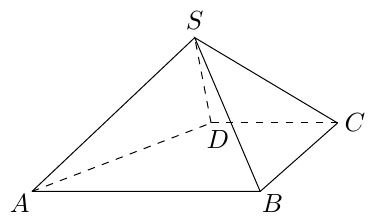
\includegraphics[width=7.4cm]{GaoKao/images/2011/syllabus_science/q19_fig1.png}
\end{center}

        \item 设数列 \(\{a_{n}\}\) 满足 \(a_1 = 0\) 且 \(\frac{1}{1 - a_{n + 1}} -\frac{1}{1 - a_n} = 1\).
\begin{enumerate}
\item 求 \( \{a_{n}\} \) 的通项公式；
\item 设 \( b_n = \frac{1 - \sqrt{a_{n+1}}}{\sqrt{n}} \)，记 \( S_n = \sum_{k=1}^{n} b_k \)，证明：\( S_n < 1 \).
\end{enumerate}

        \item 已知 \(O\) 为坐标原点，\(F\) 为椭圆 \(C: x^2 + \frac{y^2}{2} = 1\) 在 \(y\) 轴正半轴上的焦点，过 \(F\) 且斜率为 \(-\sqrt{2}\) 的直线 \(l\) 与 \(C\) 交于 \(A\)，\(B\) 两点，点 \(P\) 满足 \(\overrightarrow{OA} + \overrightarrow{OB} + \overrightarrow{OP} = 0\).
\begin{enumerate}
\item 证明：点 \(P\) 在 \(C\) 上；
\item 设点 \(P\) 关于点 \(O\) 的对称点为 \(Q\)，证明： \(A\)，\(P\)，\(B\)，\(Q\) 四点在同一圆上.
\end{enumerate}
\begin{center}
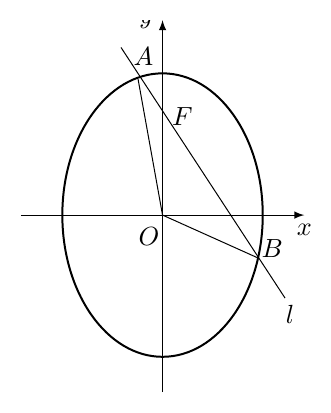
\includegraphics[width=5.5cm]{GaoKao/images/2011/syllabus_science/q21_fig1.png}
\end{center}

    \end{enumerate}

\end{description}

\begin{description}

    \item[四、选考题]

    \begin{enumerate}[leftmargin=5pt]

      \addtocounter{enumi}{+21}

        \item [A]
设函数 \( f(x) = \ln (1 + x) - \frac{2x}{x + 2} \). 证明：当 \( x > 0 \) 时，\( f(x) > 0 \).

        \item [B]
从编号 \(1\) 到 \(100\) 的 \(100\) 张卡片中每次随机抽取一张，然后放回，用这种方式连续抽取 \(20\) 次. 设抽得的 \(20\) 个号码互不相同的概率为 \(p\). 证明：\(p < \left(\frac{9}{10}\right)^{19} < \frac{1}{{\mathrm{e}}^2}\).

    \end{enumerate}

\end{description}


\subsection{2011年大纲卷（文）}\label{gk:2011年大纲卷（文）}

\begin{description}

    \item[一、选择题]

    \begin{enumerate}[leftmargin=5pt]

        \item 设集合 \(U=\{1,2,3,4\}\)，\(M=\{1,2,3\}\)，\(N=\{2,3,4\}\)，则 \(\complement_U(M\cap N)=\)（\quad）

        {\centering\begin{tabular*}{\linewidth}{@{}@{\extracolsep{\fill}}llll@{}}
          \text{A. }\(\{1,2\}\)  &  \text{B. }\(\{2,3\}\)  &  \text{C. }\(\{2,4\}\)  &  \text{D. }\(\{1,4\}\)
        \end{tabular*}\par}

        \item 函数 \(y=2\sqrt{x}\)（\(x\geqslant0\)）的反函数为（\quad）

        {\centering\begin{tabular*}{\linewidth}{@{}@{\extracolsep{\fill}}llll@{}}
          \text{A. }\(y=\frac{x^2}{4}\)（\(x\in\mathbb{R}\)）  &  \text{B. }\(y=\frac{x^2}{4}\)（\(x\geqslant0\)）  &  \text{C. }\(y=4x^2\)（\(x\in\mathbb{R}\)）  &  \text{D. }\(y=4x^2\)（\(x\geqslant0\)）
        \end{tabular*}\par}

        \item 设向量 \(\bm{a}\)，\(\bm{b}\) 满足 \(|\bm{a}|=|\bm{b}|=1\)，\(\bm{a}\cdot\bm{b}=-\frac{1}{2}\)，则 \(|\bm{a}+2\bm{b}|=\)（\quad）

        {\centering\begin{tabular*}{\linewidth}{@{}@{\extracolsep{\fill}}llll@{}}
          \text{A. }\(\sqrt{2}\)  &  \text{B. }\(\sqrt{3}\)  &  \text{C. }\(\sqrt{5}\)  &  \text{D. }\(\sqrt{7}\)
        \end{tabular*}\par}

        \item 若变量 \(x\)，\(y\) 满足约束条件
\(\begin{cases}
x+y\leqslant6,\\
x-3y\leqslant-2,\\
x\geqslant1
\end{cases}\)，则 \(z=2x+3y\) 的最小值为（\quad）

        {\centering\begin{tabular*}{\linewidth}{@{}@{\extracolsep{\fill}}llll@{}}
          \text{A. }\(17\)  &  \text{B. }\(14\)  &  \text{C. }\(5\)  &  \text{D. }\(3\)
        \end{tabular*}\par}

        \item 下面四个条件中，使 \(a>b\) 成立的充分而不必要的条件是（\quad）

        {\centering\begin{tabular*}{\linewidth}{@{}@{\extracolsep{\fill}}llll@{}}
          \text{A. }\(a>b+1\)  &  \text{B. }\(a>b-1\)  &  \text{C. }\(a^2>b^2\)  &  \text{D. }\(a^3>b^3\)
        \end{tabular*}\par}

        \item 设 \(S_n\) 为等差数列 \(\{a_n\}\) 的前 \(n\) 项和. 若 \(a_1=1\)，公差 \(d=2\)，\(S_{k+2}-S_k=24\)，则 \(k=\)（\quad）

        {\centering\begin{tabular*}{\linewidth}{@{}@{\extracolsep{\fill}}llll@{}}
          \text{A. }\(8\)  &  \text{B. }\(7\)  &  \text{C. }\(6\)  &  \text{D. }\(5\)
        \end{tabular*}\par}

        \item 设函数 \(f(x)=\cos\omega x\)（\(\omega>0\)），将 \(y=f(x)\) 的图象向右平移 \(\frac{\pi}{3}\) 个单位长度后，所得的图象与原图象重合，则 \(\omega\) 的最小值等于（\quad）

        {\centering\begin{tabular*}{\linewidth}{@{}@{\extracolsep{\fill}}llll@{}}
          \text{A. }\(\frac{1}{3}\)  &  \text{B. }\(3\)  &  \text{C. }\(6\)  &  \text{D. }\(9\)
        \end{tabular*}\par}

        \item 已知直二面角 \(\alpha-l-\beta\)，点 \(A\in\alpha\)，\(AC\perp l\)，\(C\) 为垂足，点 \(B\in\beta\)，\(BD\perp l\)，\(D\) 为垂足. 若 \(AB=2\)，\(AC=BD=1\)，则 \(CD=\)（\quad）

        {\centering\begin{tabular*}{\linewidth}{@{}@{\extracolsep{\fill}}llll@{}}
          \text{A. }\(2\)  &  \text{B. }\(\sqrt{3}\)  &  \text{C. }\(\sqrt{2}\)  &  \text{D. }\(1\)
        \end{tabular*}\par}

        \item \(4\) 位同学每人从甲，乙，丙 \(3\) 门课程中选修 \(1\) 门，则恰有 \(2\) 人选修课程甲的不同选法共有（\quad）

        {\centering\begin{tabular*}{\linewidth}{@{}@{\extracolsep{\fill}}llll@{}}
          \text{A. }\(12\) 种  &  \text{B. }\(24\) 种  &  \text{C. }\(30\) 种  &  \text{D. }\(36\) 种
        \end{tabular*}\par}

        \item 设 \(f(x)\) 是周期为 \(2\) 的奇函数，当 \(0\leqslant x\leqslant1\) 时，\(f(x)=2x(1-x)\)，则 \(f\left(-\frac{5}{2}\right)=\)（\quad）

        {\centering\begin{tabular*}{\linewidth}{@{}@{\extracolsep{\fill}}llll@{}}
          \text{A. }\(-\frac{1}{2}\)  &  \text{B. }\(-\frac{1}{4}\)  &  \text{C. }\(\frac{1}{4}\)  &  \text{D. }\(\frac{1}{2}\)
        \end{tabular*}\par}

        \item 设两圆 \(C_1\)，\(C_2\) 都和两坐标轴相切，且都过点 \((4,1)\)，则两圆心的距离 \(|C_1C_2|=\)（\quad）

        {\centering\begin{tabular*}{\linewidth}{@{}@{\extracolsep{\fill}}llll@{}}
          \text{A. }\(4\)  &  \text{B. }\(4\sqrt{2}\)  &  \text{C. }\(8\)  &  \text{D. }\(8\sqrt{2}\)
        \end{tabular*}\par}

        \item 已知平面 \(\alpha\) 截一球面得圆 \(M\)，过圆心 \(M\) 且与 \(\alpha\) 成 \(60^{\circ}\) 二面角的平面 \(\beta\) 截该球面得圆 \(N\). 若该球面的半径为 \(4\)，圆 \(M\) 的面积为 \(4\pi\)，则圆 \(N\) 的面积为（\quad）

        {\centering\begin{tabular*}{\linewidth}{@{}@{\extracolsep{\fill}}llll@{}}
          \text{A. }\(7\pi\)  &  \text{B. }\(9\pi\)  &  \text{C. }\(11\pi\)  &  \text{D. }\(13\pi\)
        \end{tabular*}\par}

    \end{enumerate}

\end{description}

\begin{description}

    \item[二、填空题]

    \begin{enumerate}[leftmargin=5pt]

      \addtocounter{enumi}{+12}

        \item \((1-x)^{10}\) 的二项展开式中，\(x\) 的系数与 \(x^9\) 的系数之差为\rule[-0.3ex]{3em}{0.4pt}.

        \item 已知 \(\alpha\in\left(\pi,\frac{3\pi}{2}\right)\)，\(\tan\alpha=2\)，则 \(\cos\alpha=\)\rule[-0.3ex]{3em}{0.4pt}.

        \item 已知正方体 \(ABCD-A_1B_1C_1D_1\) 中，\(E\) 为 \(C_1D_1\) 的中点，则异面直线 \(AE\) 与 \(BC\) 所成角的余弦值为\rule[-0.3ex]{3em}{0.4pt}.

        \item 已知 \(F_1\)，\(F_2\) 分别为双曲线 \(C:\frac{x^2}{9}-\frac{y^2}{27}=1\) 的左，右焦点，点 \(A\in C\)，点 \(M\) 的坐标为 \((2,0)\). \(AM\) 为 \(\angle F_1AF_2\) 的平分线. 则 \(|AF_2|=\)\rule[-0.3ex]{3em}{0.4pt}.

    \end{enumerate}

\end{description}

\begin{description}

    \item[三、解答题]

    \begin{enumerate}[leftmargin=5pt]

      \addtocounter{enumi}{+16}

        \item 设等比数列 \(\{a_n\}\) 的前 \(n\) 项和为 \(S_n\)，已知 \(a_2=6\)，\(6a_1+a_3=30\)，求 \(a_n\) 和 \(S_n\).

        \item \(\triangle ABC\) 的内角 \(A\)，\(B\)，\(C\) 的对边分别为 \(a\)，\(b\)，\(c\). 已知 \(a\sin A+c\sin C-\sqrt{2}a\sin C=b\sin B\).

\begin{enumerate}
\item 求 \(B\)；
\item 若 \(A=75^{\circ}\)，\(b=2\)，求 \(a\)，\(c\).
\end{enumerate}

        \item 根据以往统计资料，某地车主购买甲种保险的概率为 \(0.5\)，购买乙种保险但不购买甲种保险的概率为 \(0.3\). 设各车主购买保险相互独立.

\begin{enumerate}
\item 求该地 \(1\) 位车主至少购买甲，乙两种保险中的 \(1\) 种的概率；
\item 求该地 \(3\) 位车主中恰有 \(1\) 位车主甲，乙两种保险都不购买的概率.
\end{enumerate}

        \item 如图，四棱锥 \(S-ABCD\) 中，\(AB\parallel CD\)，\(BC\perp CD\)，侧面 \(SAB\) 为等边三角形. \(AB=BC=2\)，\(CD=SD=1\).

\begin{enumerate}
\item 证明：\(SD\perp\) 平面 \(SAB\)；
\item 求 \(AB\) 与平面 \(SBC\) 所成角的大小.
\end{enumerate}

\begin{center}
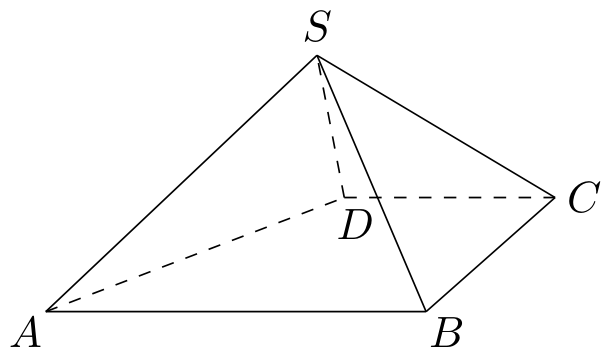
\includegraphics[width=7.1cm]{GaoKao/images/2011/syllabus_liberal/q20_fig1.png}
\end{center}

        \item 已知函数 \(f(x)=x^3+3ax^2+(3-6a)x+12a-4\)（\(a\in\mathbb{R}\)）.

\begin{enumerate}
\item 证明：曲线 \(y=f(x)\) 在 \(x=0\) 处的切线过点 \((2,2)\)；
\item 若 \(f(x)\) 在 \(x=x_0\) 处取得极小值，\(x_0\in(1,3)\)，求 \(a\) 的取值范围.
\end{enumerate}

    \end{enumerate}

\end{description}

\begin{description}

    \item[四、选考题]

    \begin{enumerate}[leftmargin=5pt]

      \addtocounter{enumi}{+21}

        \item \textbf{【选修4-1：几何证明选讲】}

已知 \(O\) 为坐标原点，\(F\) 为椭圆 \(C:x^2+\frac{y^2}{2}=1\) 在 \(y\) 轴正半轴上的焦点，过 \(F\) 且斜率为 \(-\sqrt{2}\) 的直线 \(l\) 与 \(C\) 交于 \(A\)，\(B\) 两点，点 \(P\) 满足 \(\overrightarrow{OA}+\overrightarrow{OB}+\overrightarrow{OP}=0\).

\begin{enumerate}
\item 证明：点 \(P\) 在 \(C\) 上；
\item 设点 \(P\) 关于点 \(O\) 的对称点为 \(Q\)，证明：\(A\)，\(P\)，\(B\)，\(Q\) 四点在同一圆上.
\end{enumerate}

\begin{center}
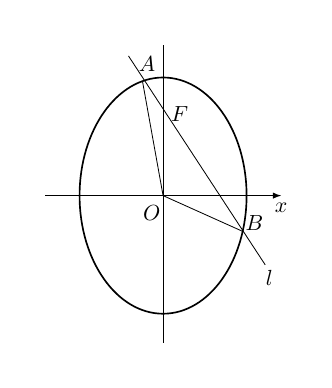
\includegraphics[width=6.0cm]{GaoKao/images/2011/syllabus_liberal/q22_fig1.png}
\end{center}

    \end{enumerate}

\end{description}


\subsection{2011年全国卷（理）}\label{gk:2011年全国卷（理）}

\begin{description}

    \item[一、选择题]

    \begin{enumerate}[leftmargin=5pt]

        \item 复数 \(\frac{2 + \i}{1 - 2\i}\) 的共轭复数是（\quad）

        {\centering\begin{tabular*}{\linewidth}{@{}@{\extracolsep{\fill}}llll@{}}
          \text{A. }\(-\frac{3}{5}\i\)  &  \text{B. }\(\frac{3}{5}\i\)  &  \text{C. }\(-\i\)  &  \text{D. }\(\i\)
        \end{tabular*}\par}

        \item 下列函数中，既是偶函数又在 \(\left(0, +\infty\right)\) 单调递增的函数是（\quad）

        {\centering\begin{tabular*}{\linewidth}{@{}@{\extracolsep{\fill}}llll@{}}
          \text{A. }\(y = x^{3}\)  &  \text{B. }\(y = |x| + 1\)  &  \text{C. }\(y = -x^{2} + 1\)  &  \text{D. }\(y = 2^{-|x|}\)
        \end{tabular*}\par}

        \item 执行如图的程序框图，如果输入的 \(N\) 是 \(6\)，那么输出的 \(p\) 是（\quad）

\begin{center}
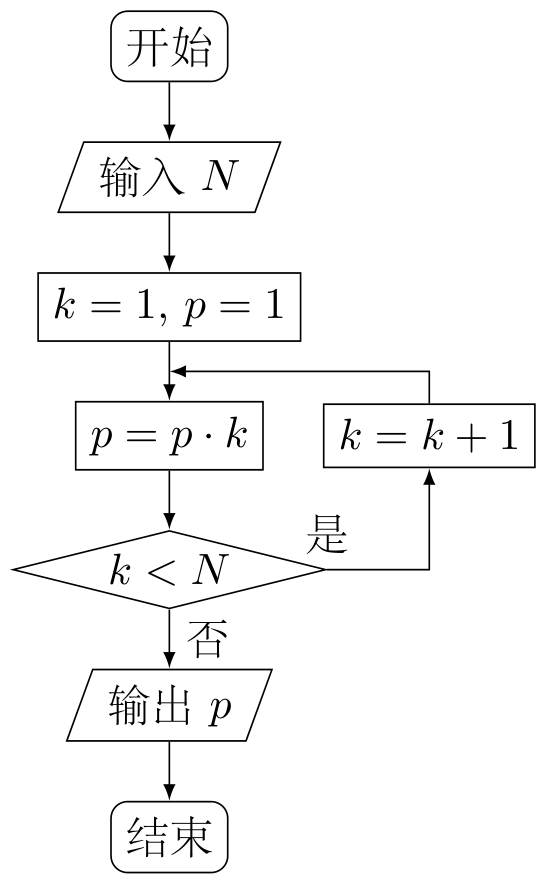
\includegraphics[width=3.2cm]{GaoKao/images/2011/new_curriculum_science/q3_fig1.png}
\end{center}

        {\centering\begin{tabular*}{\linewidth}{@{}@{\extracolsep{\fill}}llll@{}}
          \text{A. }\(120\)  &  \text{B. }\(720\)  &  \text{C. }\(1440\)  &  \text{D. }\(5040\)
        \end{tabular*}\par}

        \item 有 \(3\) 个兴趣小组，甲，乙两位同学各自参加其中一个小组，每位同学参加各个小组的可能性相同，则这两位同学参加同一个兴趣小组的概率为（\quad）

        {\centering\begin{tabular*}{\linewidth}{@{}@{\extracolsep{\fill}}llll@{}}
          \text{A. }\(\frac{1}{3}\)  &  \text{B. }\(\frac{1}{2}\)  &  \text{C. }\(\frac{2}{3}\)  &  \text{D. }\(\frac{3}{4}\)
        \end{tabular*}\par}

        \item 已知角 \(\theta\) 的顶点与原点重合，始边与 \(x\) 轴的正半轴重合，终边在直线 \(y = 2x\) 上，则 \(\cos 2\theta =\)（\quad）

        {\centering\begin{tabular*}{\linewidth}{@{}@{\extracolsep{\fill}}llll@{}}
          \text{A. }\(-\frac{4}{5}\)  &  \text{B. }\(-\frac{3}{5}\)  &  \text{C. }\(\frac{3}{5}\)  &  \text{D. }\(\frac{4}{5}\)
        \end{tabular*}\par}

        \item 在一个几何体的三视图中，正视图和俯视图如下图所示，则相应的侧视图可以为（\quad）

\begin{center}
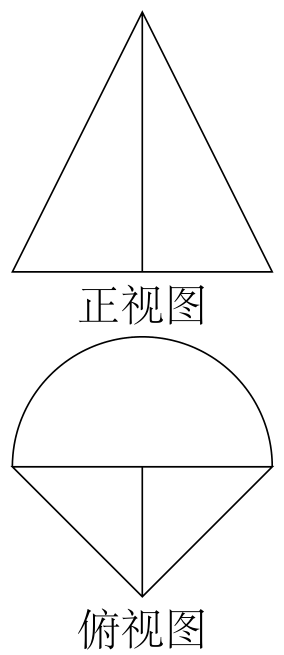
\includegraphics[width=2.8cm]{GaoKao/images/2011/new_curriculum_science/q6_condition.png}
\end{center}

        {\centering\begin{tabular*}{\linewidth}{@{}@{\extracolsep{\fill}}cccc@{}}
          \text{A. }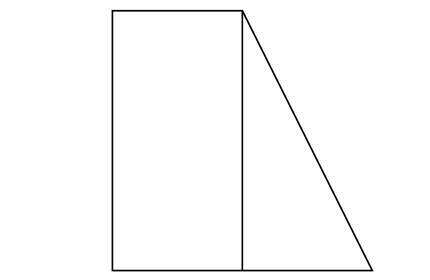
\includegraphics[width=0.15\paperwidth]{GaoKao/images/2011/new_curriculum_science/q6_optA.png}  &  \text{B. }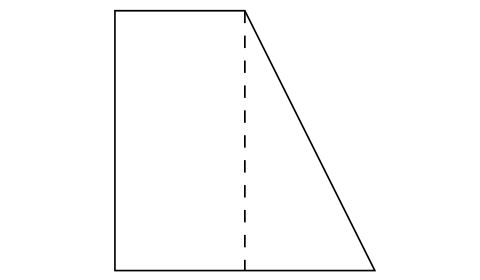
\includegraphics[width=0.15\paperwidth]{GaoKao/images/2011/new_curriculum_science/q6_optB.png}  &  \text{C. }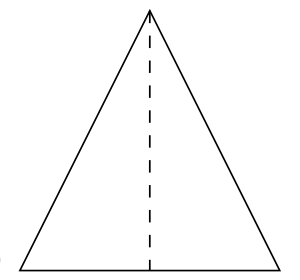
\includegraphics[width=0.15\paperwidth]{GaoKao/images/2011/new_curriculum_science/q6_optC.png}  &  \text{D. }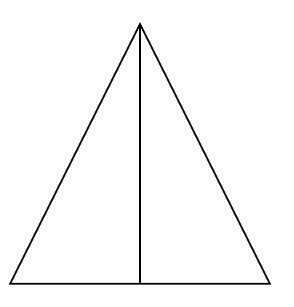
\includegraphics[width=0.15\paperwidth]{GaoKao/images/2011/new_curriculum_science/q6_optD.png}
        \end{tabular*}\par}

        \item 设直线 \(l\) 过双曲线 \(C\) 的一个焦点，且与 \(C\) 的一条对称轴垂直，\(l\) 与 \(C\) 交于 \(A\)，\(B\) 两点，\(|AB|\) 为 \(C\) 的实轴长的 \(2\) 倍，则 \(C\) 的离心率为（\quad）

        {\centering\begin{tabular*}{\linewidth}{@{}@{\extracolsep{\fill}}llll@{}}
          \text{A. }\(\sqrt{2}\)  &  \text{B. }\(\sqrt{3}\)  &  \text{C. }\(2\)  &  \text{D. }\(3\)
        \end{tabular*}\par}

        \item \(\left(x + \frac{a}{x}\right)\left(2x - \frac{1}{x}\right)^5\) 的展开式中各项系数的和为 \(2\)，则该展开式中常数项为（\quad）

        {\centering\begin{tabular*}{\linewidth}{@{}@{\extracolsep{\fill}}llll@{}}
          \text{A. }\(-40\)  &  \text{B. }\(-20\)  &  \text{C. }\(20\)  &  \text{D. }\(40\)
        \end{tabular*}\par}

        \item 由曲线 \(y = \sqrt{x}\)，直线 \(y = x - 2\) 及 \(y\) 轴所围成的图形的面积为（\quad）

        {\centering\begin{tabular*}{\linewidth}{@{}@{\extracolsep{\fill}}llll@{}}
          \text{A. }\(\frac{10}{3}\)  &  \text{B. }\(4\)  &  \text{C. }\( \frac{16}{3} \)  &  \text{D. }\(6\)
        \end{tabular*}\par}

        \item 已知 \(\bm{a}\) 与 \(\bm{b}\) 均为单位向量，其夹角为 \(\theta\)，有下列四个命题：
\begin{enumerate}
    \item \(p_1: |\bm{a} + \bm{b}| > 1 \Leftrightarrow \theta \in \left[0, \frac{2\pi}{3}\right)\)
    \item \(p_2: |\bm{a} + \bm{b}| > 1 \Leftrightarrow \theta \in \left(\frac{2\pi}{3}, \pi\right]\)
    \item \(p_3: |\bm{a} - \bm{b}| > 1 \Leftrightarrow \theta \in \left[0, \frac{\pi}{3}\right)\)
    \item \(p_4: |\bm{a} - \bm{b}| > 1 \Leftrightarrow \theta \in \left(\frac{\pi}{3}, \pi\right]\)
\end{enumerate}
其中的真命题是（\quad）

        {\centering\begin{tabular*}{\linewidth}{@{}@{\extracolsep{\fill}}llll@{}}
          \text{A. }\(p_1\)，\(p_4\)  &  \text{B. }\(p_1\)，\(p_3\)  &  \text{C. }\(p_2\)，\(p_3\)  &  \text{D. }\(p_2\)，\(p_4\)
        \end{tabular*}\par}

        \item 设函数 \( f(x) = \sin\left(\omega x + \varphi\right) + \cos\left(\omega x + \varphi\right) \)（\(\omega > 0\)，\(|\varphi| < \frac{\pi}{2}\)）的最小正周期为 \( \pi \)，且 \( f(-x) = f(x) \)，则（\quad）

        {\centering\begin{tabular*}{\linewidth}{@{}@{\extracolsep{\fill}}llll@{}}
          \text{A. }\(f(x)\) 在 \(\left(0, \frac{\pi}{2}\right)\) 单调递减  &  \text{B. }\(f(x)\) 在 \(\left(\frac{\pi}{4}, \frac{3\pi}{4}\right)\) 单调递减  &  \text{C. }\(f(x)\) 在 \(\left(0, \frac{\pi}{2}\right)\) 单调递增  &  \text{D. }\(f(x)\) 在 \(\left(\frac{\pi}{4}, \frac{3\pi}{4}\right)\) 单调递增
        \end{tabular*}\par}

        \item 函数 \( y = \frac{1}{1 - x} \) 的图象与函数 \( y = 2\sin \pi x \)（\(-2 \leqslant x \leqslant 4\)）的图象所有交点的横坐标之和等于（\quad）

        {\centering\begin{tabular*}{\linewidth}{@{}@{\extracolsep{\fill}}llll@{}}
          \text{A. }\(2\)  &  \text{B. }\(4\)  &  \text{C. }\(6\)  &  \text{D. }\(8\)
        \end{tabular*}\par}

    \end{enumerate}

\end{description}

\begin{description}

    \item[二、填空题]

    \begin{enumerate}[leftmargin=5pt]

      \addtocounter{enumi}{+12}

        \item 若变量 \(x\)，\(y\) 满足约束条件 \(\begin{cases}
3 \leqslant 2x + y \leqslant 9,\\
6 \leqslant x - y \leqslant 9.
\end{cases}\) 则 \(z = x + 2y\) 的最小值为\rule[-0.3ex]{3em}{0.4pt}.

        \item 在平面直角坐标系 \(xOy\) 中，椭圆 \(C\) 的中心为原点，焦点 \(F_{1}\)，\(F_{2}\) 在 \(x\) 轴上，离心率为 \(\frac{\sqrt{2}}{2}\)，过 \(F_{1}\) 的直线 \(l\) 交 \(C\) 于 \(A\)，\(B\) 两点，且 \(\triangle ABF_{2}\) 的周长为 \(16\)，那么 \(C\) 的方程为\rule[-0.3ex]{3em}{0.4pt}.

        \item 已知矩形 \(ABCD\) 的顶点都在半径为 \(4\) 的球 \(O\) 的球面上，且 \(AB = 6\)，\(BC = 2\sqrt{3}\)，则棱锥 \(O - ABCD\) 的体积为\rule[-0.3ex]{3em}{0.4pt}.

        \item 在 \(\triangle ABC\) 中，\(B = 60^{\circ}\)，\(AC = \sqrt{3}\)，则 \(AB + 2BC\) 的最大值为\rule[-0.3ex]{3em}{0.4pt}.

    \end{enumerate}

\end{description}

\begin{description}

    \item[三、解答题]

    \begin{enumerate}[leftmargin=5pt]

      \addtocounter{enumi}{+16}

        \item 等比数列 \(\{a_{n}\}\) 的各项均为正数，且 \(2a_{1} + 3a_{2} = 1\)，\(a_{3}^{2} = 9a_{2}a_{6}\).
\begin{enumerate}
\item 求数列 \( \{a_{n}\} \) 的通项公式；
\item 设 \( b_{n} = \log_{3}a_{1} + \log_{3}a_{2} + \cdots + \log_{3}a_{n} \)，求数列 \( \left\{\frac{1}{b_{n}}\right\} \) 的前 \( n \) 项和.
\end{enumerate}

        \item 如图，四棱锥 \(P - ABCD\) 中，底面 \(ABCD\) 为平行四边形，\(\angle DAB = 60^{\circ}\)，\(AB = 2AD\)，\(PD \perp\) 底面 \(ABCD\).
\begin{enumerate}
\item 证明： \(PA \perp BD\)；
\item 若 \(PD = AD\)，求二面角 \(A - PB - C\) 的余弦值.
\end{enumerate}

\begin{center}
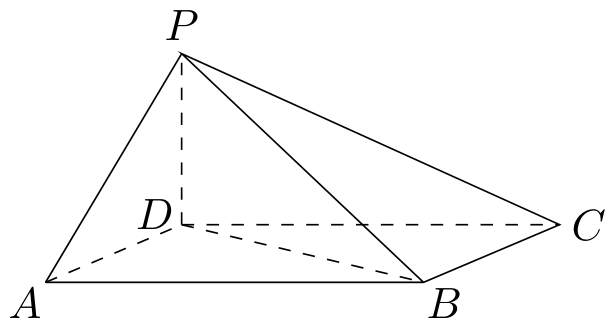
\includegraphics[width=7.6cm]{GaoKao/images/2011/new_curriculum_science/q18_fig1.png}
\end{center}

        \item 某种产品的质量以其质量指标值衡量，质量指标值越大表明质量越好，且质量指标值大于或等于 \(102\) 的产品为优质品. 现用两种新配方（分别称为 A 配方和 B 配方）做试验，各生产了 \(100\) 件这种产品，并测量了每件产品的质量指标值，得到了下面试验结果：

\begin{center}
A 配方的频数分布表

\begin{tabular}{c|c|c|c|c|c}
\hline
指标值分组 & \(\left[90,94\right)\) & \(\left[94,98\right)\) & \(\left[98,102\right)\) & \(\left[102,106\right)\) & \(\left[106,110\right]\) \\
\hline
频数 & \(8\) & \(20\) & \(42\) & \(22\) & \(8\) \\
\hline
\end{tabular}

B 配方的频数分布表

\begin{tabular}{c|c|c|c|c|c}
\hline
指标值分组 & \(\left[90,94\right)\) & \(\left[94,98\right)\) & \(\left[98,102\right)\) & \(\left[102,106\right)\) & \(\left[106,110\right]\) \\
\hline
频数 & \(4\) & \(12\) & \(42\) & \(32\) & \(10\) \\
\hline
\end{tabular}
\end{center}

\begin{enumerate}
\item 分别估计用 A 配方，B 配方生产的产品的优质品率；
\item 已知用 B 配方生产一件产品的利润 \(y\)（单位：元）与其质量指标值 \(t\) 的关系式为 \( y = \begin{cases}
-2, & t < 94,\\
2, & 94 \leqslant t < 102,\\
4, & t \geqslant 102.
\end{cases} \) 从用 B 配方生产的产品中任取一件，其利润记为 \(X\)（单位：元），求 \(X\) 的分布列及数学期望. （以实验结果中质量指标值落入各组的频率作为一件产品的质量指标值落入相应组的概率）.
\end{enumerate}

        \item 在平面直角坐标系 \(xOy\) 中，已知点 \(A\left(0, -1\right)\)，\(B\) 点在直线 \(y = -3\) 上，\(M\) 点满足 \(\overrightarrow{MB} \parallel \overrightarrow{OA}\)，\(\overrightarrow{MA} \cdot \overrightarrow{AB} = \overrightarrow{MB} \cdot \overrightarrow{BA}\)，\(M\) 点的轨迹为曲线 \(C\).
\begin{enumerate}
\item 求 \(C\) 的方程；
\item \(P\) 为 \(C\) 上的动点，\(l\) 为 \(C\) 在 \(P\) 点处的切线，求 \(O\) 点到 \(l\) 距离的最小值.
\end{enumerate}

        \item 已知函数 \( f(x) = a \frac{\ln x}{x + 1} + \frac{b}{x} \)，曲线 \( y = f(x) \) 在点 \(\left(1, f(1)\right)\) 处的切线方程为 \( x + 2y - 3 = 0 \).
\begin{enumerate}
    \item 求 \(a\)，\(b\) 的值；
\item 如果当 \(x > 0\)，且 \(x \neq 1\) 时，\(f(x) > \frac{\ln x}{x - 1} + \frac{k}{x}\)，求 \(k\) 的取值范围.
\end{enumerate}

        \item 如图，\(D\)，\(E\) 分别为 \(\triangle ABC\) 的边 \(AB\)，\(AC\) 上的点，且不与 \(\triangle ABC\) 的顶点重合. 已知 \(AE\) 的长为 \(m\)，\(AC\) 的长为 \(n\)，\(AD\)，\(AB\) 的长是关于 \(x\) 的方程 \(x^{2} - 14x + mn = 0\) 的两个根.
\begin{enumerate}
\item 证明： \(C\)，\(B\)，\(D\)，\(E\) 四点共圆；
\item 若 \(\angle A = 90^{\circ}\)，且 \(m = 4\)，\(n = 6\)，求 \(C\)，\(B\)，\(D\)，\(E\) 所在圆的半径.
\end{enumerate}

\begin{center}
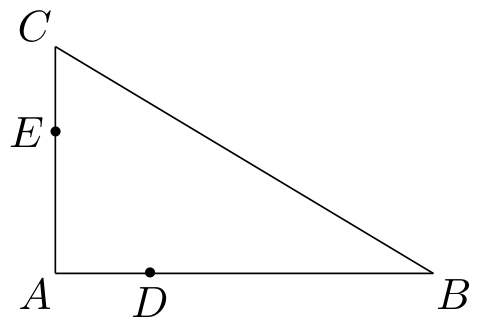
\includegraphics[width=5.9cm]{GaoKao/images/2011/new_curriculum_science/q22_fig1.png}
\end{center}

        \item 在直角坐标系 \(xOy\) 中，曲线 \(C_1\) 的参数方程为 \(\begin{cases}
x = 2\cos \alpha,\\
y = 2 + 2\sin \alpha,
\end{cases}\)（\(\alpha\) 为参数），\(M\) 是 \(C_1\) 上的动点，\(P\) 点满足 \(\overrightarrow{OP} = 2\overrightarrow{OM}\)，\(P\) 点的轨迹为曲线 \(C_2\).
\begin{enumerate}
\item 求 \(C_2\) 的方程；
\item 在以 \(O\) 为极点，\(x\) 轴的正半轴为极轴的极坐标系中，射线 \(\theta = \frac{\pi}{3}\) 与 \(C_1\) 的异于极点的交点为 \(A\)，与 \(C_2\) 的异于极点的交点为 \(B\)，求 \(|AB|\).
\end{enumerate}

        \item 设函数 \(f(x)=|x-a|+3x\)，其中 \(a>0\).
\begin{enumerate}
\item 当 \(a=1\) 时，求不等式 \(f(x)\geqslant 3x+2\) 的解集；
\item 若不等式 \(f(x)\leqslant 0\) 的解集为 \(\{x\mid x\leqslant -1\}\)，求 \(a\) 的值.
\end{enumerate}

    \end{enumerate}

\end{description}


\subsection{2011年全国卷（文）}\label{gk:2011年全国卷（文）}

\begin{description}

    \item[一、选择题]

    \begin{enumerate}[leftmargin=5pt]

        \item 已知集合 \(M = \{0, 1, 2, 3, 4\}\)，\(N = \{1, 3, 5\}\)，\(P = M \cap N\)，则 \(P\) 的子集共有（\quad）

        {\centering\begin{tabular*}{\linewidth}{@{}@{\extracolsep{\fill}}llll@{}}
          \text{A. }\(2\) 个  &  \text{B. }\(4\) 个  &  \text{C. }\(6\) 个  &  \text{D. }\(8\) 个
        \end{tabular*}\par}

        \item 复数 \(\frac{5\i}{1 - 2\i} =\)（\quad）

        {\centering\begin{tabular*}{\linewidth}{@{}@{\extracolsep{\fill}}llll@{}}
          \text{A. }\(2 - \i\)  &  \text{B. }\(1 - 2\i\)  &  \text{C. }\(-2 + \i\)  &  \text{D. }\(-1 + 2\i\)
        \end{tabular*}\par}

        \item 下列函数中，既是偶函数又在 \((0, +\infty)\) 单调递增的函数是（\quad）

        {\centering\begin{tabular*}{\linewidth}{@{}@{\extracolsep{\fill}}llll@{}}
          \text{A. }\(y = x^{3}\)  &  \text{B. }\(y = |x| + 1\)  &  \text{C. }\(y = -x^{2} + 1\)  &  \text{D. }\(y = 2^{-|x|}\)
        \end{tabular*}\par}

        \item 椭圆 \(\frac{x^2}{16} + \frac{y^2}{8} = 1\) 的离心率为（\quad）

        {\centering\begin{tabular*}{\linewidth}{@{}@{\extracolsep{\fill}}llll@{}}
          \text{A. }\( \frac{1}{3} \)  &  \text{B. }\( \frac{1}{2} \)  &  \text{C. }\( \frac{\sqrt{3}}{3} \)  &  \text{D. }\(\frac{\sqrt{2}}{2}\)
        \end{tabular*}\par}

        \item 执行如图的程序框图，如果输入的 \(N\) 是 6，那么输出的 \(p\) 是（\quad）

\begin{center}
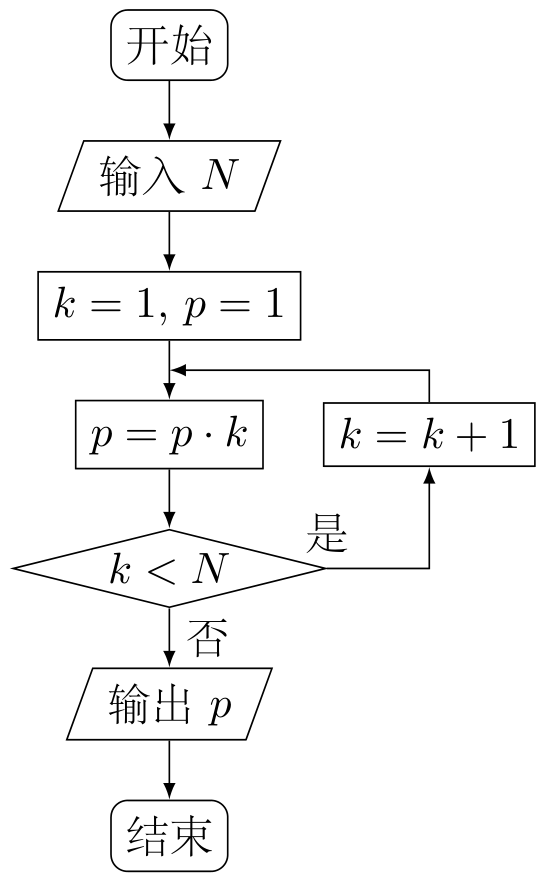
\includegraphics[width=5.1cm]{GaoKao/images/2011/new_curriculum_liberal/q5_flowchart.png}
\end{center}

        {\centering\begin{tabular*}{\linewidth}{@{}@{\extracolsep{\fill}}llll@{}}
          \text{A. }\(120\)  &  \text{B. }\(720\)  &  \text{C. }\(1440\)  &  \text{D. }\(5040\)
        \end{tabular*}\par}

        \item 有 \(3\) 个兴趣小组，甲，乙两位同学各自参加其中一个小组，每位同学参加各个小组的可能性相同，则这两位同学参加同一个兴趣小组的概率为（\quad）

        {\centering\begin{tabular*}{\linewidth}{@{}@{\extracolsep{\fill}}llll@{}}
          \text{A. }\( \frac{1}{3} \)  &  \text{B. }\( \frac{1}{2} \)  &  \text{C. }\( \frac{2}{3} \)  &  \text{D. }\( \frac{3}{4} \)
        \end{tabular*}\par}

        \item 已知角 \(\theta\) 的顶点与原点重合，始边与 \(x\) 轴的正半轴重合，终边在直线 \(y = 2x\) 上，则 \(\cos 2\theta =\)（\quad）

        {\centering\begin{tabular*}{\linewidth}{@{}@{\extracolsep{\fill}}llll@{}}
          \text{A. }\(-\frac{1}{5}\)  &  \text{B. }\(-\frac{3}{5}\)  &  \text{C. }\( \frac{3}{5} \)  &  \text{D. }\( \frac{4}{5} \)
        \end{tabular*}\par}

        \item 在一个几何体的三视图中，正视图和俯视图如下图所示，则相应的侧视图可以为（\quad）

\begin{center}
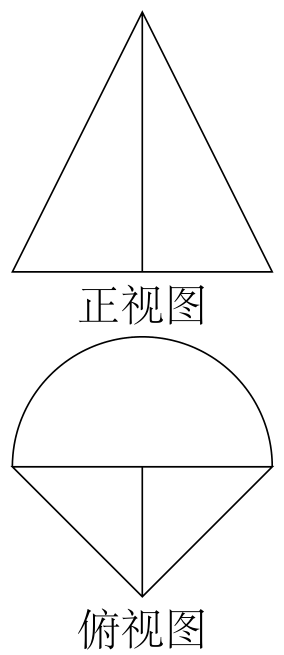
\includegraphics[width=2.8cm]{GaoKao/images/2011/new_curriculum_liberal/q8_condition.png}
\end{center}

        {\centering\begin{tabular*}{\linewidth}{@{}@{\extracolsep{\fill}}cccc@{}}
          \text{A. }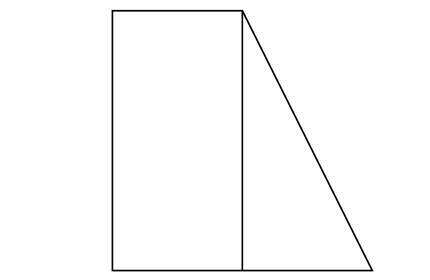
\includegraphics[width=0.15\paperwidth]{GaoKao/images/2011/new_curriculum_liberal/q8_optA.png}  &  \text{B. }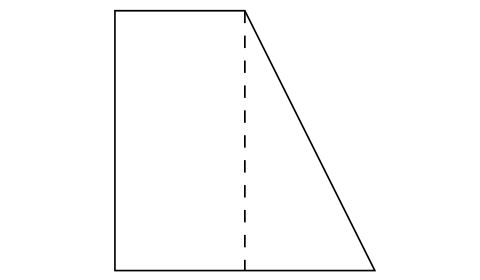
\includegraphics[width=0.15\paperwidth]{GaoKao/images/2011/new_curriculum_liberal/q8_optB.png}  &  \text{C. }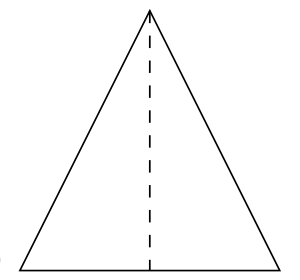
\includegraphics[width=0.15\paperwidth]{GaoKao/images/2011/new_curriculum_liberal/q8_optC.png}  &  \text{D. }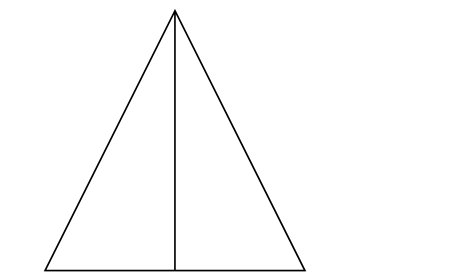
\includegraphics[width=0.15\paperwidth]{GaoKao/images/2011/new_curriculum_liberal/q8_optD.png}
        \end{tabular*}\par}

        \item 已知直线 \(l\) 过抛物线 \(C\) 的焦点，且与 \(C\) 的对称轴垂直，\(l\) 与 \(C\) 交于 \(A, B\) 两点，\( \left|AB\right|=12 \)，\(P\) 为 \(C\) 的准线上一点，则 \( \triangle ABP \) 的面积为（\quad）

        {\centering\begin{tabular*}{\linewidth}{@{}@{\extracolsep{\fill}}llll@{}}
          \text{A. }\(18\)  &  \text{B. }\(24\)  &  \text{C. }\(36\)  &  \text{D. }\(48\)
        \end{tabular*}\par}

        \item 在下列区间中，函数 \( f(x) = {\mathrm{e}}^{x} + 4x - 3 \) 的零点所在的区间为（\quad）

        {\centering\begin{tabular*}{\linewidth}{@{}@{\extracolsep{\fill}}llll@{}}
          \text{A. }\(\left(-\frac{1}{4}, 0\right)\)  &  \text{B. }\(\left(0, \frac{1}{4}\right)\)  &  \text{C. }\(\left(\frac{1}{4}, \frac{1}{2}\right)\)  &  \text{D. }\(\left(\frac{1}{2}, \frac{3}{4}\right)\)
        \end{tabular*}\par}

        \item 设函数 \( f(x) = \sin \left(2x + \frac{\pi}{4}\right) + \cos \left(2x + \frac{\pi}{4}\right) \)，则（\quad）

        {\centering\begin{tabular*}{\linewidth}{@{}@{\extracolsep{\fill}}llll@{}}
          \text{A. }\(y = f(x)\) 在 \(\left(0, \frac{\pi}{2}\right)\) 单调递增，其图象关于直线 \(x = \frac{\pi}{4}\) 对称  &  \text{B. }\(y = f(x)\) 在 \(\left(0, \frac{\pi}{2}\right)\) 单调递增，其图象关于直线 \(x = \frac{\pi}{2}\) 对称  &  \text{C. }\(y = f(x)\) 在 \(\left(0, \frac{\pi}{2}\right)\) 单调递减，其图象关于直线 \(x = \frac{\pi}{4}\) 对称  &  \text{D. }\( y = f(x) \) 在 \( \left(0, \frac{\pi}{2}\right) \) 单调递减，其图象关于直线 \( x = \frac{\pi}{2} \) 对称
        \end{tabular*}\par}

        \item 已知函数 \( y = f(x) \) 的周期为 2，当 \( x \in [-1, 1] \) 时 \( f(x) = x^2 \)，那么函数 \( y = f(x) \) 的图象与函数 \( y = | \lg x | \) 的图象的交点共有（\quad）

        {\centering\begin{tabular*}{\linewidth}{@{}@{\extracolsep{\fill}}llll@{}}
          \text{A. }\(10\) 个  &  \text{B. }\(9\) 个  &  \text{C. }\(8\) 个  &  \text{D. }\(1\) 个
        \end{tabular*}\par}

    \end{enumerate}

\end{description}

\begin{description}

    \item[二、填空题]

    \begin{enumerate}[leftmargin=5pt]

      \addtocounter{enumi}{+12}

        \item 已知 \(\bm{a}\) 与 \(\bm{b}\) 为两个不共线的单位向量，\(k\) 为实数，若向量 \(\bm{a} + \bm{b}\) 与向量 \(k\bm{a} - \bm{b}\) 垂直，则 \(k = \)\rule[-0.3ex]{3em}{0.4pt}.

        \item 若变量 \(x\)，\(y\) 满足约束条件 \(\begin{cases}
3 \leqslant 2x + y \leqslant 9,\\
6 \leqslant x - y \leqslant 9,
\end{cases}\) 则 \(z = x + 2y\) 的最小值为\rule[-0.3ex]{3em}{0.4pt}.

        \item \(\triangle ABC\) 中，\(B = 120^{\circ}\)，\(AC = 7\)，\(AB = 5\)，则 \(\triangle ABC\) 的面积为\rule[-0.3ex]{3em}{0.4pt}.

        \item 已知两个圆锥有公共底面，且两圆锥的顶点和底面的圆周都在同一个球面上. 若圆锥底面面积是这个球面面积的 \(\frac{3}{16}\)，则这两个圆锥中，体积较小者的高与体积较大的高的比值为\rule[-0.3ex]{3em}{0.4pt}.

    \end{enumerate}

\end{description}

\begin{description}

    \item[三、解答题]

    \begin{enumerate}[leftmargin=5pt]

      \addtocounter{enumi}{+16}

        \item 已知等比数列 \(\{a_{n}\}\) 中，\(a_{1} = \frac{1}{3}\)，公比 \(q = \frac{1}{3}\).
\begin{enumerate}
\item 若 \(S_{n}\) 为 \(\{a_{n}\}\) 的前 \(n\) 项和，证明： \(S_{n} = \frac{1 - a_{n}}{2}\)；
\item 设 \(b_{n} = \log_{3} a_{1} + \log_{3} a_{2} + \cdots + \log_{3} a_{n}\)，求数列 \(\{b_{n}\}\) 的通项公式.
\end{enumerate}

        \item 如图，四棱锥 \(P - ABCD\) 中，底面 \(ABCD\) 为平行四边形，\(\angle DAB = 60^{\circ}\)，\(AB = 2AD\)，\(PD \perp\) 底面 \(ABCD\).
\begin{enumerate}
\item 证明： \(PA \perp BD\)；
\item 设 \(PD = AD = 1\)，求棱锥 \(D - PBC\) 的高.
\end{enumerate}

\begin{center}
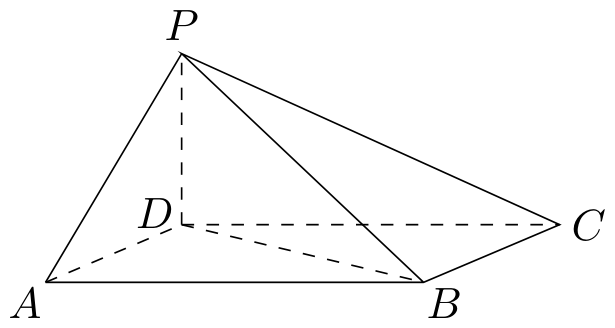
\includegraphics[width=7.6cm]{GaoKao/images/2011/new_curriculum_liberal/q18_pyramid.png}
\end{center}

        \item 某种产品的质量以其质量指标值衡量，质量指标值越大表明质量越好，且质量指标值大于或等于 \(102\) 的产品为优质品. 现用两种新配方（分别称为 A 配方和 B 配方）做试验，各生产了 \(100\) 件这种产品，并测量了每件产品的质量指标值，得到了下面试验结果：

\begin{center}
A 配方的频数分布表

\begin{tabular}{c|ccccc}
\hline
指标值分组 & \(\left[90,94\right)\) & \(\left[94,98\right)\) & \(\left[98,102\right)\) & \(\left[102,106\right)\) & \(\left[106,110\right]\) \\
\hline
频数 & \(8\) & \(20\) & \(42\) & \(22\) & \(8\) \\
\hline
\end{tabular}

B 配方的频数分布表

\begin{tabular}{c|ccccc}
\hline
指标值分组 & \(\left[90,94\right)\) & \(\left[94,98\right)\) & \(\left[98,102\right)\) & \(\left[102,106\right)\) & \(\left[106,110\right]\) \\
\hline
频数 & \(4\) & \(12\) & \(42\) & \(32\) & \(10\) \\
\hline
\end{tabular}
\end{center}

\begin{enumerate}
\item 分别估计用 A 配方，B 配方生产的产品优质品率；
\item 已知用 B 配方生产一件产品的利润 \(y\)（单位：元）与其质量指标值 \(t\) 的关系式为 \(y = \begin{cases}
-2,  t < 94,\\
2,  94 \leqslant t < 102,\\
4,  t \geqslant 102.
\end{cases}\)
估计用 B 配方生产的一件产品的利润大于 \(0\) 的概率，并求用 B 配方生产的上述 \(100\) 件产品平均一件的利润.
\end{enumerate}

        \item 在平面直角坐标系 \(xOy\) 中，曲线 \(y = x^{2} - 6x + 1\) 与坐标轴的交点都在圆 \(C\) 上.
\begin{enumerate}
\item 求圆 \(C\) 的方程；
\item 若圆 \(C\) 与直线 \(x - y + a = 0\) 交于 \(A, B\) 两点，且 \(OA \perp OB\)，求 \(a\) 的值.
\end{enumerate}

        \item 已知函数 \( f(x) = a \frac{\ln x}{x + 1} + \frac{b}{x} \)，曲线 \( y = f(x) \) 在点 \((1, f(1))\) 处的切线方程为 \( x + 2y - 3 = 0 \).
\begin{enumerate}
\item 求 \(a, b\) 的值；
\item 证明：当 \(x > 0\)，且 \(x \neq 1\) 时，\(f(x) > \frac{\ln x}{x - 1}\).
\end{enumerate}

        \item 如图，\(D\)，\(E\) 分别为 \(\triangle ABC\) 的边 \(AB\)，\(AC\) 上的点，且不与 \(\triangle ABC\) 的顶点重合.
已知 \(AE\) 的长为 \(m\)，\(AC\) 的长为 \(n\)，\(AD\)，\(AB\) 的长是关于 \(x\) 的方程 \(x^{2} - 14x + mn = 0\) 的两个根.
\begin{enumerate}
\item 证明： \(C\)，\(B\)，\(D\)，\(E\) 四点共圆；
\item 若 \(\angle A = 90^{\circ}\)，且 \(m = 4\)，\(n = 6\)，求 \(C\)，\(B\)，\(D\)，\(E\) 所在圆的半径.
\end{enumerate}

\begin{center}
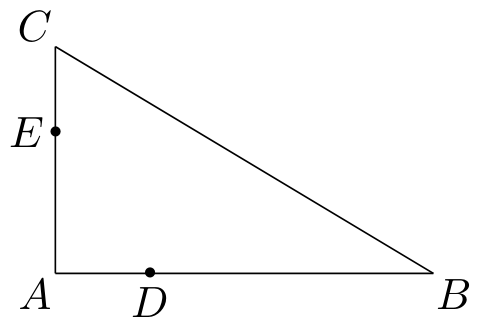
\includegraphics[width=5.9cm]{GaoKao/images/2011/new_curriculum_liberal/q22_triangle.png}
\end{center}

        \item 在直角坐标系 \(xOy\) 中，曲线 \(C_1\) 的参数方程为 \(\begin{cases}
x = 2\cos \alpha,\\
y = 2 + 2\sin \alpha,
\end{cases}\)（\(\alpha\) 为参数），\(M\) 是 \(C_1\) 上的动点，\(P\) 点满足 \(\overrightarrow{OP} = 2\overrightarrow{OM}\)，\(P\) 点的轨迹为曲线 \(C_2\).
\begin{enumerate}
\item 求 \(C_2\) 的方程；
\item 在以 \(O\) 为极点，\(x\) 轴的正半轴为极轴的极坐标系中，射线 \( \theta = \frac{\pi}{3} \) 与 \(C_1\) 的异于极点的交点为 \(A\)，与 \(C_2\) 的异于极点的交点为 \(B\)，求 \(|AB|\).
\end{enumerate}

        \item 设函数 \( f(x) = |x - a| + 3x \)，其中 \( a > 0 \).
\begin{enumerate}
\item 当 \(a = 1\) 时，求不等式 \(f(x) \geqslant 3x + 2\) 的解集；
\item 若不等式 \( f(x) \leqslant 0 \) 的解集为 \( \{x \mid x \leqslant -1\} \)，求 \( a \) 的值.
\end{enumerate}

    \end{enumerate}

\end{description}


\subsection{2011年安徽卷（理）}\label{gk:2011年安徽卷（理）}

\begin{description}

    \item[一、选择题]

    \begin{enumerate}[leftmargin=5pt]

        \item 设 \(\i\) 是虚数单位，复数 \(\frac{1 + a\i}{2 - \i}\) 为纯虚数，则实数 \(a\) 为（\quad）

        {\centering\begin{tabular*}{\linewidth}{@{}@{\extracolsep{\fill}}llll@{}}
          \text{A. }2  &  \text{B. }\(-2\)  &  \text{C. }\(-\frac{1}{2}\)  &  \text{D. }\(\frac{1}{2}\)
        \end{tabular*}\par}

        \item 双曲线 \(2x^{2} - y^{2} = 8\) 的实轴长是（\quad）

        {\centering\begin{tabular*}{\linewidth}{@{}@{\extracolsep{\fill}}llll@{}}
          \text{A. }2  &  \text{B. }\(2\sqrt{2}\)  &  \text{C. }4  &  \text{D. }\(4\sqrt{2}\)
        \end{tabular*}\par}

        \item 设 \( f(x) \) 是定义在 \( \mathbb{R} \) 上的奇函数，当 \( x \leqslant 0 \) 时，\( f(x) = 2x^2 - x \)，则 \( f(1) = \)（\quad）

        {\centering\begin{tabular*}{\linewidth}{@{}@{\extracolsep{\fill}}llll@{}}
          \text{A. }\(-3\)  &  \text{B. }\(-1\)  &  \text{C. }1  &  \text{D. }3
        \end{tabular*}\par}

        \item 设变量 \(x\)，\(y\) 满足 \(|x| + |y| \leqslant 1\)，则 \(x + 2y\) 的最大值和最小值分别为（\quad）

        {\centering\begin{tabular*}{\linewidth}{@{}@{\extracolsep{\fill}}llll@{}}
          \text{A. }1, \(-1\)  &  \text{B. }2, \(-2\)  &  \text{C. }1, \(-2\)  &  \text{D. }2, \(-1\)
        \end{tabular*}\par}

        \item 在极坐标系中，点 \(\left(2, \frac{\pi}{3}\right)\) 到圆 \(\rho = 2\cos \theta\) 的圆心的距离为（\quad）

        {\centering\begin{tabular*}{\linewidth}{@{}@{\extracolsep{\fill}}llll@{}}
          \text{A. }2  &  \text{B. }\(\sqrt{4 + \frac{\pi^2}{9}}\)  &  \text{C. }\(\sqrt{1 + \frac{\pi^2}{9}}\)  &  \text{D. }\(\sqrt{3}\)
        \end{tabular*}\par}

        \item 一个空间几何体的三视图如图所示，则该几何体的表面积为（\quad）

\begin{center}
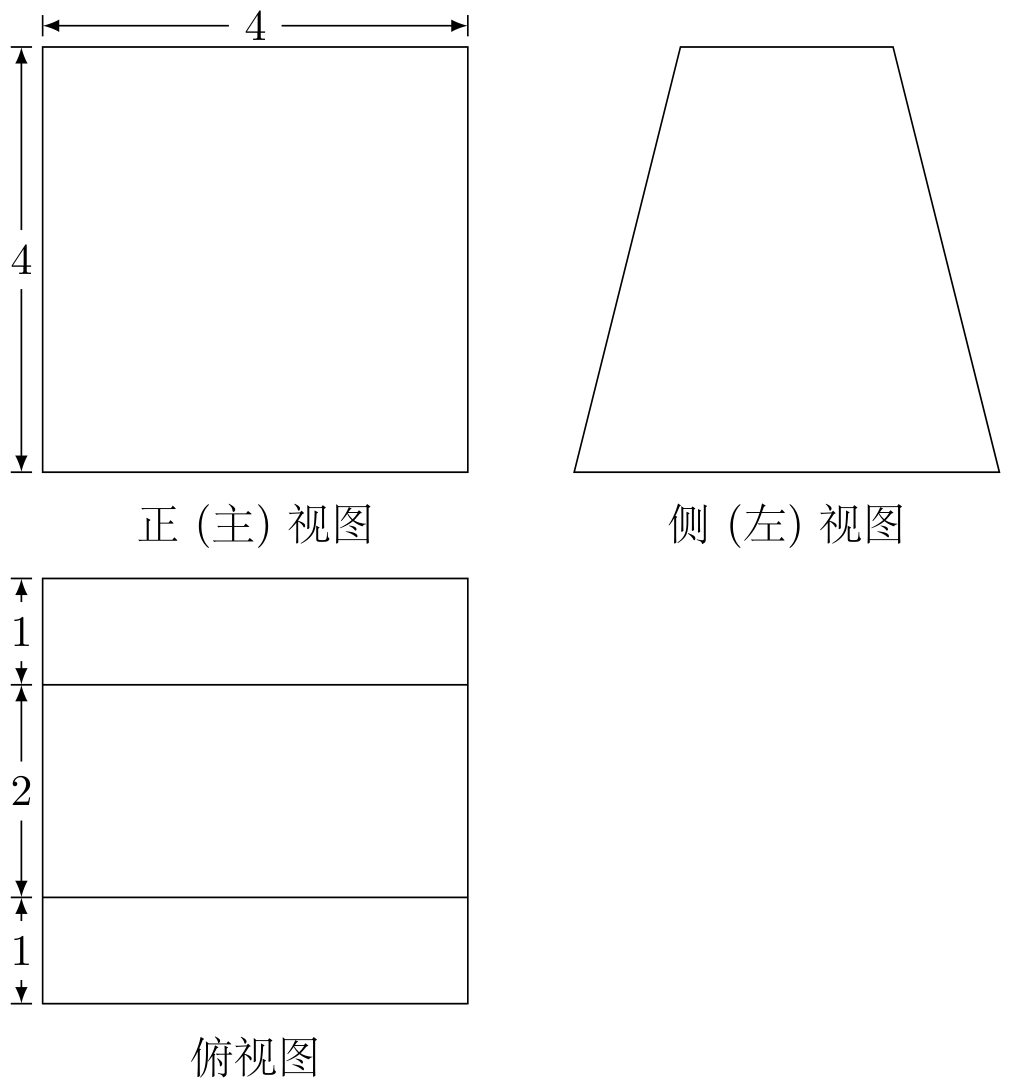
\includegraphics[width=9.9cm]{GaoKao/images/2011/anhui_science/q6_fig1.png}
\end{center}

        {\centering\begin{tabular*}{\linewidth}{@{}@{\extracolsep{\fill}}llll@{}}
          \text{A. }48  &  \text{B. }\(32 + 8\sqrt{17}\)  &  \text{C. }\(48 + 8\sqrt{17}\)  &  \text{D. }80
        \end{tabular*}\par}

        \item 命题“所有能被 2 整除的整数都是偶数”的否定是（\quad）

        {\centering\begin{tabular*}{\linewidth}{@{}@{\extracolsep{\fill}}llll@{}}
          \text{A. }所有不能被 2 整除的整数都是偶数  &  \text{B. }所有能被 2 整除的整数都不是偶数  &  \text{C. }存在一个不能被 2 整除的整数是偶数  &  \text{D. }存在一个能被 2 整除的整数不是偶数
        \end{tabular*}\par}

        \item 设集合 \(A = \{1, 2, 3, 4, 5, 6\}\)，\(B = \{4, 5, 6, 7, 8\}\)，则满足 \(S \subseteq A\) 且 \(S \cap B \neq \varnothing\) 的集合 \(S\) 的个数是（\quad）

        {\centering\begin{tabular*}{\linewidth}{@{}@{\extracolsep{\fill}}llll@{}}
          \text{A. }57  &  \text{B. }56  &  \text{C. }49  &  \text{D. }8
        \end{tabular*}\par}

        \item 已知函数 \( f(x) = \sin (2x + \varphi) \)，其中 \( \varphi \) 为实数，若 \( f(x) \leqslant \left|f\left(\frac{\pi}{6}\right)\right| \) 对 \( x \in \mathbb{R} \) 恒成立，且 \( f\left(\frac{\pi}{2}\right) > f(\pi) \)，则 \( f(x) \) 的单调递增区间是（\quad）

        {\centering\begin{tabular*}{\linewidth}{@{}@{\extracolsep{\fill}}llll@{}}
          \text{A. }\(\left[k\pi - \frac{\pi}{3}, k\pi + \frac{\pi}{6}\right]\)（\(k \in \mathbb{Z}\)）  &  \text{B. }\(\left[k\pi, k\pi + \frac{\pi}{2}\right]\)（\(k \in \mathbb{Z}\)）  &  \text{C. }\(\left[k\pi + \frac{\pi}{6}, k\pi + \frac{2\pi}{3}\right]\)（\(k \in \mathbb{Z}\)）  &  \text{D. }\(\left[k\pi - \frac{\pi}{2}, k\pi\right]\)（\(k \in \mathbb{Z}\)）
        \end{tabular*}\par}

        \item 函数 \( f(x) = ax^{m}(1 - x)^n \) 在区间 \([0,1]\) 上的图象如图所示，则 \(m\)，\(n\) 的值可能是（\quad）

\begin{center}
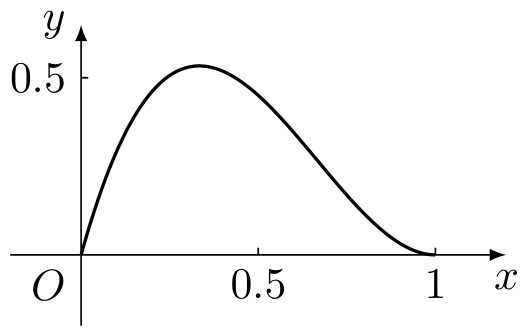
\includegraphics[width=5.0cm]{GaoKao/images/2011/anhui_science/q10_fig1.png}
\end{center}

        {\centering\begin{tabular*}{\linewidth}{@{}@{\extracolsep{\fill}}llll@{}}
          \text{A. }\(m = 1, n = 1\)  &  \text{B. }\(m = 1\)，\(n = 2\)  &  \text{C. }\(m = 2\)，\(n = 1\)  &  \text{D. }\(m = 3\)，\(n = 1\)
        \end{tabular*}\par}

    \end{enumerate}

\end{description}

\begin{description}

    \item[二、填空题]

    \begin{enumerate}[leftmargin=5pt]

      \addtocounter{enumi}{+10}

        \item 如图所示，程序框图（算法流程图）的输出结果是\rule[-0.3ex]{3em}{0.4pt}.

\begin{center}
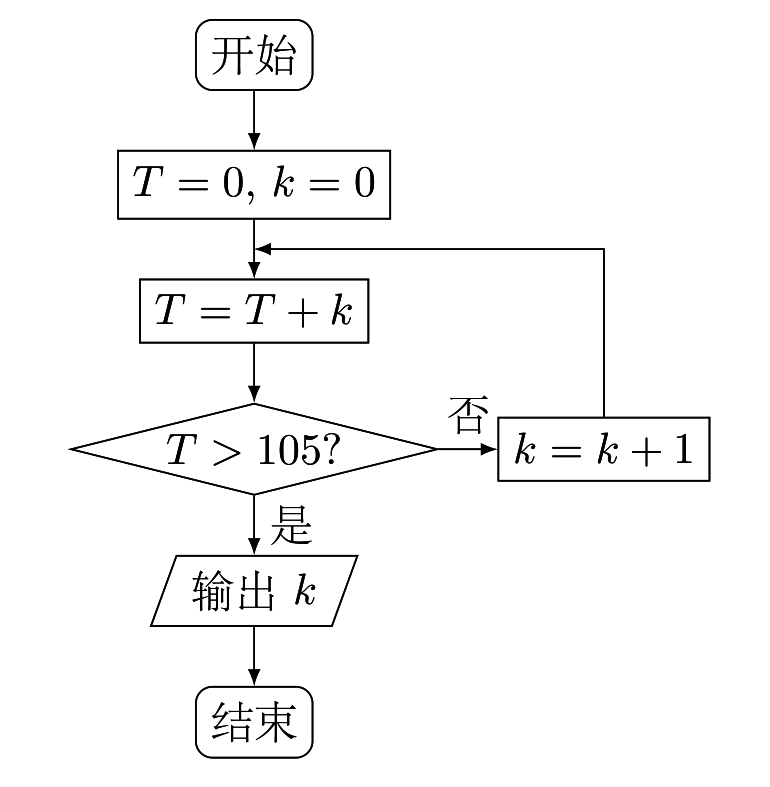
\includegraphics[width=0.42\linewidth]{GaoKao/images/2011/anhui_science/q11_fig1.png}
\end{center}

        \item 设 \((x - 1)^{21} = a_0 + a_1x + a_2x^2 + \dots + a_{21}x^{21}\)，则 \(a_{10} + a_{11} =\rule[-0.3ex]{3em}{0.4pt}\).

        \item 已知向量 \(\bm{a}\)，\(\bm{b}\) 满足 \((\bm{a} + 2\bm{b}) \cdot (\bm{a} - \bm{b}) = -6\)，且 \(|\bm{a}| = 1\)，\(|\bm{b}| = 2\)，则 \(\bm{a}\) 与 \(\bm{b}\) 的夹角为\rule[-0.3ex]{3em}{0.4pt}.

        \item 已知 \(\triangle ABC\) 的一个内角为 \(120^{\circ}\)，并且三边长构成公差为 4 的等差数列，则 \(\triangle ABC\) 的面积为\rule[-0.3ex]{3em}{0.4pt}.

        \item 在平面直角坐标系中，如果 \(x\) 与 \(y\) 都是整数，就称点 \((x, y)\) 为整点，下列命题中正确的是\rule[-0.3ex]{3em}{0.4pt}.（写出所有正确命题的编号）

\begin{enumerate}
\item 存在这样的直线，既不与坐标轴平行又不经过任何整点；
\item 如果 \(k\) 与 \(b\) 都是无理数，则直线 \(y = kx + b\) 不经过任何整点；
\item 直线 \(l\) 经过无穷多个整点，当且仅当 \(l\) 经过两个不同的整点；
\item 直线 \(y = kx + b\) 经过无穷多个整点的充分必要条件是：\(k\) 与 \(b\) 都是有理数；
\item 存在恰经过一个整点的直线.
\end{enumerate}

    \end{enumerate}

\end{description}

\begin{description}

    \item[三、解答题]

    \begin{enumerate}[leftmargin=5pt]

      \addtocounter{enumi}{+15}

        \item 设 \( f(x) = \frac{{\mathrm{e}}^x}{1 + ax^2} \)，其中 \( a \) 为正实数.

\begin{enumerate}
\item 当 \(a=\frac{4}{3}\) 时，求 \( f(x) \) 的极值点；
\item 若 \( f(x) \) 为 \( \mathbb{R} \) 上的单调函数，求 \( a \) 的取值范围.
\end{enumerate}

        \item 如图，\(ABEDFC\) 为多面体，平面 \(ABED\) 与平面 \(ACFD\) 垂直，点 \(O\) 在线段 \(AD\) 上，\(OA = 1\)，\(OD = 2\)，\(\triangle OAB\)，\(\triangle OAC\)，\(\triangle ODE\)，\(\triangle ODF\) 都是正三角形.

\begin{enumerate}
\item 证明直线 \(BC \parallel EF\)；
\item 求棱锥 \(F-OBED\) 的体积.
\end{enumerate}

\begin{center}
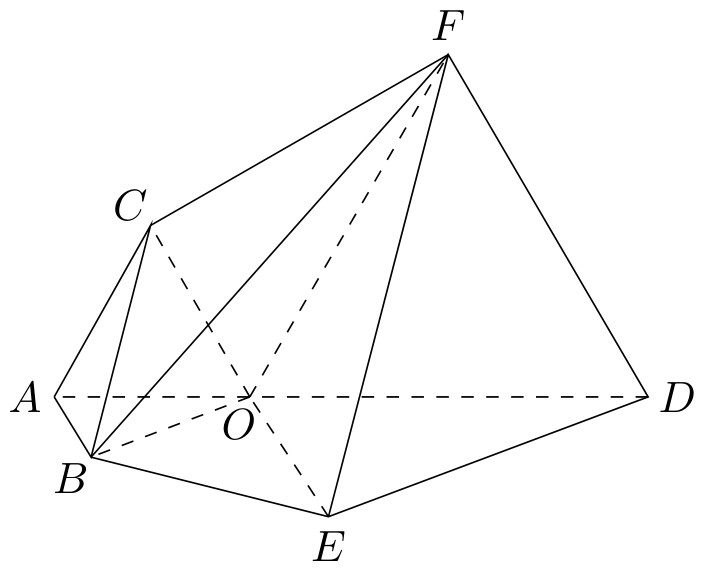
\includegraphics[width=8.2cm]{GaoKao/images/2011/anhui_science/q17_fig1.png}
\end{center}

        \item 在数 1 和 100 之间插入 \(n\) 个实数，使得这 \(n + 2\) 个数构成递增的等比数列，将这 \(n + 2\) 个数的乘积记作 \(T_{n}\)，再令 \(a_{n} = \lg T_{n}\)，\(n \geqslant 1\).

\begin{enumerate}
\item 求数列 \(\{a_{n}\}\) 的通项公式；
\item 设 \(b_{n} = \tan a_{n} \cdot \tan a_{n+1}\)，求数列 \(\{b_{n}\}\) 的前 \(n\) 项和 \(S_{n}\).
\end{enumerate}

        \item \begin{enumerate}
\item 设 \(x \geqslant 1\)，\(y \geqslant 1\)，证明 \(x + y + \frac{1}{xy} \leqslant \frac{1}{x} + \frac{1}{y} + xy\)；
\item \(1 < a \leqslant b \leqslant c\)，证明 \(\log_{a} b + \log_{b} c + \log_{c} a \leqslant \log_{b} a + \log_{c} b + \log_{a} c\).
\end{enumerate}

        \item 工作人员需进入核电站完成某项具有高辐射危险的任务，每次只派一个人进去，且每个人只派一次，工作时间不超过 10 分钟，如果前一个人 10 分钟内不能完成任务则撤出，再派下一个人. 现在一共只有甲，乙，丙三个人可派. 他们各自能完成任务的概率分别 \(p_{1}\)，\(p_{2}\)，\(p_{3}\). 假设 \(p_{1}\)，\(p_{2}\)，\(p_{3}\) 互不相等，且假定各人能否完成任务的事件相互独立.

\begin{enumerate}
\item 如果按甲最先，乙次之，丙最后的顺序派人，求任务能被完成的概率. 若改变三个人被派出的先后顺序，任务能被完成的概率是否发生变化？
\item 若按某指定顺序派人，这三个人各自能完成任务的概率依次为 \(q_{1}\)，\(q_{2}\)，\(q_{3}\)，其中 \(q_{1}\)，\(q_{2}\)，\(q_{3}\) 是 \(p_{1}\)，\(p_{2}\)，\(p_{3}\) 的一个排列. 求所需派出人员数目 \(X\) 的分布列和均值（数学期望）\(E(X)\)；
\item 假定 \(1 > p_{1} > p_{2} > p_{3}\)，试分析以怎样的先后顺序派出人员，可使所需派出的人员数目的均值（数学期望）达到最小.
\end{enumerate}

        \item 设 \(\lambda > 0\)，点 \(A\) 的坐标为 \((1,1)\)，点 \(B\) 在抛物线 \(y = x^2\) 上运动，点 \(Q\) 满足 \(\overrightarrow{BQ} = \lambda \overrightarrow{QA}\)，经过点 \(Q\) 与 \(x\) 轴垂直的直线交抛物线于点 \(M\)，点 \(P\) 满足 \(\overrightarrow{QM} = \lambda \overrightarrow{MP}\)，求点 \(P\) 的轨迹方程.

\begin{center}
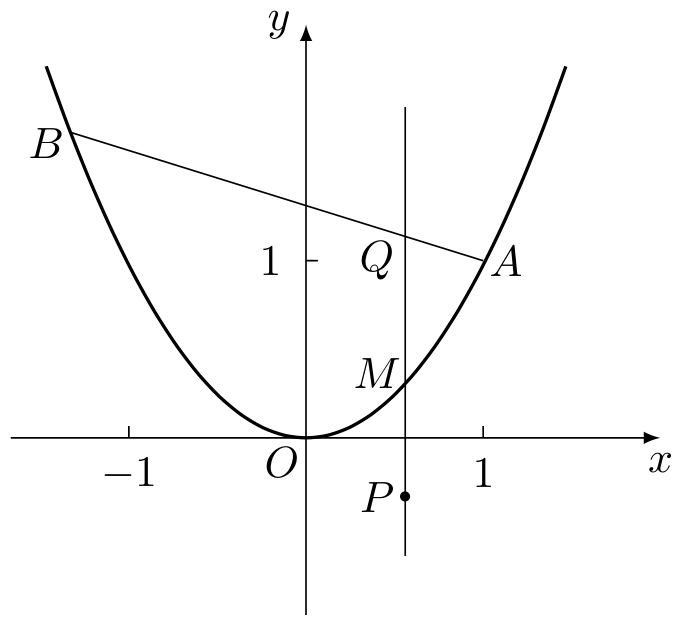
\includegraphics[width=8.5cm]{GaoKao/images/2011/anhui_science/q21_fig1.png}
\end{center}

    \end{enumerate}

\end{description}


\subsection{2011年安徽卷（文）}\label{gk:2011年安徽卷（文）}

\begin{description}

    \item[一、选择题]

    \begin{enumerate}[leftmargin=5pt]

        \item 设 \(\i\) 是虚数单位，复数 \(\frac{1 + a\i}{2 - \i}\) 为纯虚数，则实数 \(a\) 为（\quad）

        {\centering\begin{tabular*}{\linewidth}{@{}@{\extracolsep{\fill}}llll@{}}
          \text{A. }\(2\)  &  \text{B. }\(-2\)  &  \text{C. }\(-\frac{1}{2}\)  &  \text{D. }\(\frac{1}{2}\)
        \end{tabular*}\par}

        \item 集合 \(U = \{1, 2, 3, 4, 5, 6\}\)，\(S = \{1, 4, 5\}\)，\(T = \{2, 3, 4\}\)，则 \(S \cap \left(\complement_{U} T\right)\) 等于（\quad）

        {\centering\begin{tabular*}{\linewidth}{@{}@{\extracolsep{\fill}}llll@{}}
          \text{A. }\(\{1, 4, 5, 6\}\)  &  \text{B. }\(\{1, 5\}\)  &  \text{C. }\(\{4\}\)  &  \text{D. }\(\{1, 2, 3, 4, 5\}\)
        \end{tabular*}\par}

        \item 双曲线 \(2x^{2} - y^{2} = 8\) 的实轴长是（\quad）

        {\centering\begin{tabular*}{\linewidth}{@{}@{\extracolsep{\fill}}llll@{}}
          \text{A. }\(2\)  &  \text{B. }\(2\sqrt{2}\)  &  \text{C. }\(4\)  &  \text{D. }\(4\sqrt{2}\)
        \end{tabular*}\par}

        \item 若直线 \(3x + y + a = 0\) 过圆 \(x^{2} + y^{2} + 2x - 4y = 0\) 的圆心，则 \(a\) 的值为（\quad）

        {\centering\begin{tabular*}{\linewidth}{@{}@{\extracolsep{\fill}}llll@{}}
          \text{A. }\(-1\)  &  \text{B. }\(1\)  &  \text{C. }\(3\)  &  \text{D. }\(-3\)
        \end{tabular*}\par}

        \item 若点 \((a, b)\) 在 \(y = \lg x\) 图象上，\(a \neq 1\)，则下列点中在此图象上的是（\quad）

        {\centering\begin{tabular*}{\linewidth}{@{}@{\extracolsep{\fill}}llll@{}}
          \text{A. }\(\left(\frac{1}{a}, b\right)\)  &  \text{B. }\((10a, 1 - b)\)  &  \text{C. }\(\left(\frac{10}{a}, b + 1\right)\)  &  \text{D. }\((a^{2}, 2b)\)
        \end{tabular*}\par}

        \item 设变量 \(x\)，\(y\) 满足 \(\begin{cases}
x + y \leqslant 1,\\
x - y \leqslant 1,\\
x \geqslant 0,
\end{cases}\)
则 \(x + 2y\) 的最大值和最小值分别为（\quad）

        {\centering\begin{tabular*}{\linewidth}{@{}@{\extracolsep{\fill}}llll@{}}
          \text{A. }\(1\)，\(-1\)  &  \text{B. }\(2\)，\(-2\)  &  \text{C. }\(1\)，\(-2\)  &  \text{D. }\(2\)，\(-1\)
        \end{tabular*}\par}

        \item 若数列 \(\{a_{n}\}\) 的通项公式是 \(a_{n} = (-1)^{n}(3n - 2)\)，则 \(a_{1} + a_{2} + \cdots + a_{10} =\)（\quad）

        {\centering\begin{tabular*}{\linewidth}{@{}@{\extracolsep{\fill}}llll@{}}
          \text{A. }\(15\)  &  \text{B. }\(12\)  &  \text{C. }\(-12\)  &  \text{D. }\(-15\)
        \end{tabular*}\par}

        \item 一个空间几何体的三视图如图所示，则该几何体的表面积为（\quad）

\begin{center}
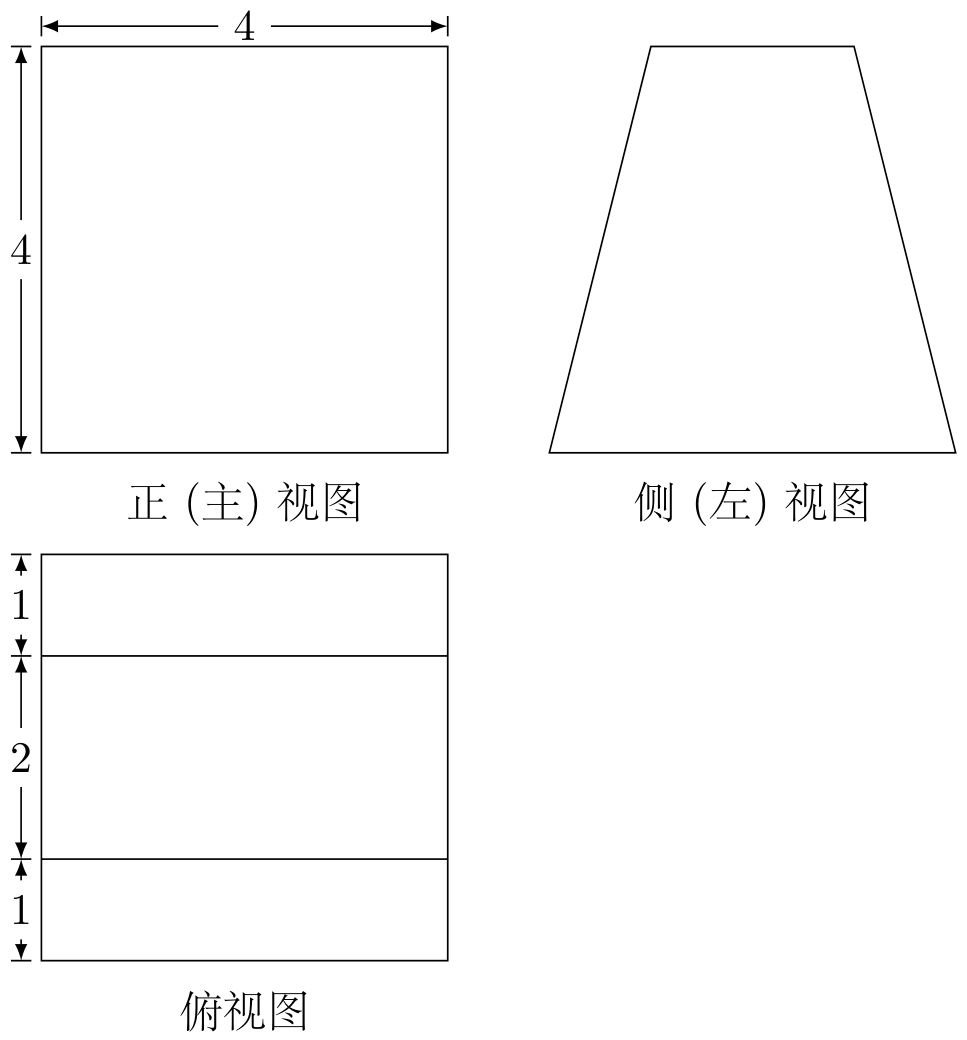
\includegraphics[width=9.5cm]{GaoKao/images/2011/anhui_liberal/q8_fig1.png}
\end{center}

        {\centering\begin{tabular*}{\linewidth}{@{}@{\extracolsep{\fill}}llll@{}}
          \text{A. }\(48\)  &  \text{B. }\(32 + 8\sqrt{17}\)  &  \text{C. }\(48 + 8\sqrt{17}\)  &  \text{D. }\(80\)
        \end{tabular*}\par}

        \item 从正六边形的 6 个顶点中随机选择 4 个顶点，则以它们作为顶点的四边形是矩形的概率等于（\quad）

        {\centering\begin{tabular*}{\linewidth}{@{}@{\extracolsep{\fill}}llll@{}}
          \text{A. }\(\frac{1}{10}\)  &  \text{B. }\(\frac{1}{8}\)  &  \text{C. }\(\frac{1}{6}\)  &  \text{D. }\(\frac{1}{5}\)
        \end{tabular*}\par}

        \item 函数 \(f(x) = ax^{n}(1 - x)^{2}\) 在区间 \([0, 1]\) 上的图象如图所示，则 \(n\) 可能是（\quad）

\begin{center}
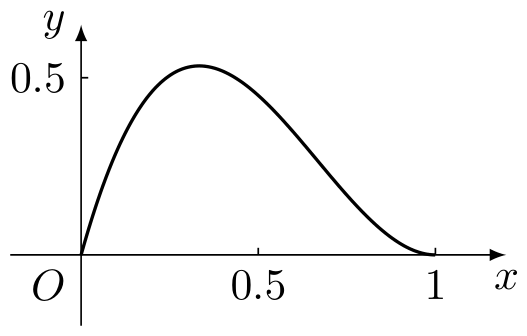
\includegraphics[width=5.0cm]{GaoKao/images/2011/anhui_liberal/q10_fig1.png}
\end{center}

        {\centering\begin{tabular*}{\linewidth}{@{}@{\extracolsep{\fill}}llll@{}}
          \text{A. }\(1\)  &  \text{B. }\(2\)  &  \text{C. }\(3\)  &  \text{D. }\(4\)
        \end{tabular*}\par}

    \end{enumerate}

\end{description}

\begin{description}

    \item[二、填空题]

    \begin{enumerate}[leftmargin=5pt]

      \addtocounter{enumi}{+10}

        \item 设 \(f(x)\) 是定义在 \(\mathbb{R}\) 上的奇函数，当 \(x \leqslant 0\) 时，\(f(x) = 2x^{2} - x\)，则 \(f(1) =\rule[-0.3ex]{3em}{0.4pt}\).

        \item 如图所示，程序框图（算法流程图）的输出结果是\rule[-0.3ex]{3em}{0.4pt}.

\begin{center}
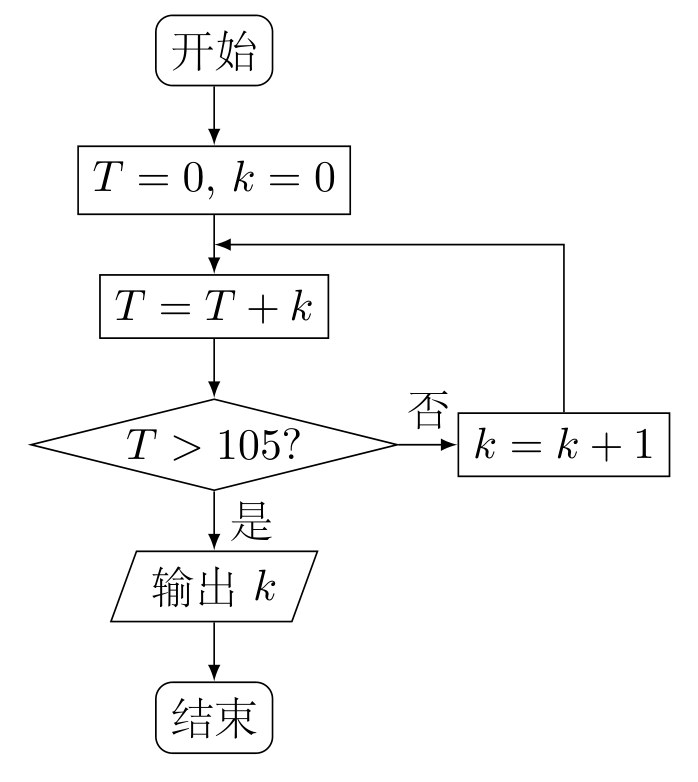
\includegraphics[width=0.5\linewidth]{GaoKao/images/2011/anhui_liberal/q12_fig1.png}
\end{center}

        \item 函数 \(y = \frac{1}{\sqrt{6 - x - x^{2}}}\) 的定义域是\rule[-0.3ex]{3em}{0.4pt}.

        \item 已知向量 \(\bm{a}\)，\(\bm{b}\) 满足 \((\bm{a} + 2\bm{b}) \cdot (\bm{a} - \bm{b}) = -6\)，且 \(|\bm{a}| = 1\)，\(|\bm{b}| = 2\)，则 \(\bm{a}\) 与 \(\bm{b}\) 的夹角为\rule[-0.3ex]{3em}{0.4pt}.

        \item 设 \(f(x) = a\sin 2x + b\cos 2x\)，其中 \(a\)，\(b \in \mathbb{R}\)，\(ab \neq 0\)，若 \(f(x) \leqslant \left|f\left(\frac{\pi}{6}\right)\right|\) 对一切 \(x \in \mathbb{R}\) 恒成立，则
\begin{enumerate}
\item \(f\left(\frac{11\pi}{12}\right) = 0\)；
\item \(f\left(\frac{7\pi}{10}\right) < \left|f\left(\frac{\pi}{5}\right)\right|\)；
\item \(f(x)\) 既不是奇函数，也不是偶函数；
\item \(f(x)\) 的单调递增区间是 \(\left[k\pi + \frac{\pi}{6}, k\pi + \frac{2\pi}{3}\right]\)（\(k \in \mathbb{Z}\)）；
\item 存在经过点 \((a, b)\) 的直线与函数 \(f(x)\) 的图象不相交.
\end{enumerate}
以上结论正确的是\rule[-0.3ex]{3em}{0.4pt}.（写出所有正确结论的编号）

    \end{enumerate}

\end{description}

\begin{description}

    \item[三、解答题]

    \begin{enumerate}[leftmargin=5pt]

      \addtocounter{enumi}{+15}

        \item 在 \(\triangle ABC\) 中，\(a\)，\(b\)，\(c\) 分别为内角 \(A\)，\(B\)，\(C\) 所对的边长，\(a = \sqrt{3}\)，\(b = \sqrt{2}\)，\(1 + 2\cos(B + C) = 0\)，求边 \(BC\) 上的高.

        \item 设直线 \(l_{1} : y = k_{1}x + 1\)，\(l_{2} : y = k_{2}x - 1\)，其中实数 \(k_{1}\)，\(k_{2}\) 满足 \(k_{1}k_{2} + 2 = 0\).
\begin{enumerate}
\item 证明 \(l_{1}\) 与 \(l_{2}\) 相交；
\item 证明 \(l_{1}\) 与 \(l_{2}\) 的交点在椭圆 \(2x^{2} + y^{2} = 1\) 上.
\end{enumerate}

        \item 设 \(f(x) = \frac{{\mathrm{e}}^{x}}{1 + ax^{2}}\)，其中 \(a\) 为正实数.
\begin{enumerate}
\item 当 \(a = \frac{4}{3}\) 时，求 \(f(x)\) 的极值点；
\item 若 \(f(x)\) 为 \(\mathbb{R}\) 上的单调函数，求 \(a\) 的取值范围.
\end{enumerate}

        \item 如图，\(ABEDFC\) 为多面体，平面 \(ABED\) 与平面 \(ACFD\) 垂直，点 \(O\) 在线段 \(AD\) 上，\(OA = 1\)，\(OD = 2\)，\(\triangle OAB\)，\(\triangle OAC\)，\(\triangle ODE\)，\(\triangle ODF\) 都是正三角形.

\begin{enumerate}
\item 证明直线 \(BC \parallel EF\)；
\item 求棱锥 \(F - OBED\) 的体积.
\end{enumerate}

\begin{center}
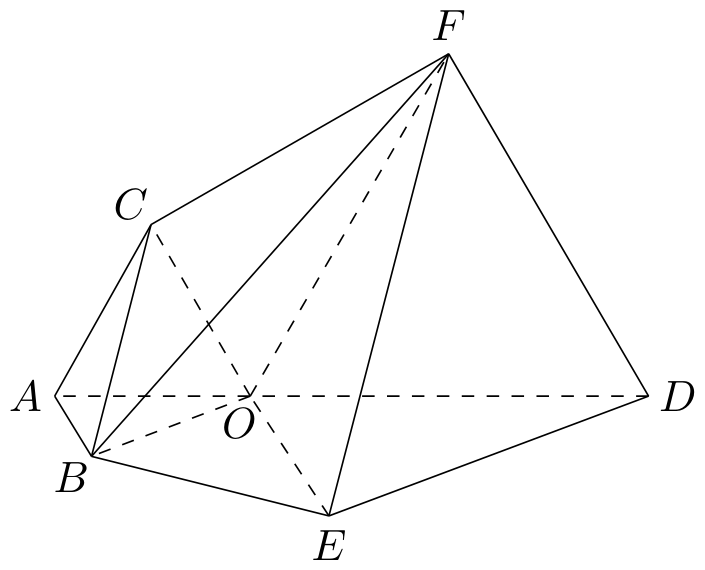
\includegraphics[width=8.8cm]{GaoKao/images/2011/anhui_liberal/q19_fig1.png}
\end{center}

        \item 某地最近十年粮食需求量逐年上升，下表是部分统计数据：

\begin{center}
\begin{tabular}{c|ccccc}
年份 & \(2002\) & \(2004\) & \(2006\) & \(2008\) & \(2010\) \\
\hline
需求量（\(\text{万吨}\)） & \(236\) & \(246\) & \(257\) & \(276\) & \(286\)
\end{tabular}
\end{center}

\begin{enumerate}
\item 利用所给数据求年需求量与年份之间的回归直线方程 \(\hat{y} = bx + a\)；
\item 利用（1）中所求出的直线方程预测该地 \(2012\) 年的粮食需求量.
\end{enumerate}

        \item 在数 \(1\) 和 \(100\) 之间插入 \(n\) 个实数，使得这 \(n + 2\) 个数构成递增的等比数列，将这 \(n + 2\) 个数的乘积记作 \(T_{n}\)，再令 \(a_{n} = \lg T_{n}\)，\(n \geqslant 1\).
\begin{enumerate}
\item 求数列 \(\{a_{n}\}\) 的通项公式；
\item 设 \(b_{n} = \tan a_{n} \cdot \tan a_{n+1}\)，求数列 \(\{b_{n}\}\) 的前 \(n\) 项和 \(S_{n}\).
\end{enumerate}

    \end{enumerate}

\end{description}


\subsection{2011年北京卷（理）}\label{gk:2011年北京卷（理）}

\begin{description}

    \item[一、选择题]

    \begin{enumerate}[leftmargin=5pt]

        \item 已知集合 \(P = \{x \mid x^2 \leqslant 1\}\)，\(M = \{a\}\). 若 \(P \cup M = P\)，则 \(a\) 的取值范围是（\quad）

        {\centering\begin{tabular*}{\linewidth}{@{}@{\extracolsep{\fill}}llll@{}}
          \text{A. }\((- \infty, -1]\)  &  \text{B. }\([1, +\infty)\)  &  \text{C. }\([-1, 1]\)  &  \text{D. }\((- \infty, -1] \cup [1, +\infty)\)
        \end{tabular*}\par}

        \item 复数 \(\frac{\i-2}{1+2\i}=\)（\quad）

        {\centering\begin{tabular*}{\linewidth}{@{}@{\extracolsep{\fill}}llll@{}}
          \text{A. }\(\i\)  &  \text{B. }\(-\i\)  &  \text{C. }\(-\frac{4}{5} - \frac{3}{5}\i\)  &  \text{D. }\(-\frac{4}{5} + \frac{3}{5}\i\)
        \end{tabular*}\par}

        \item 在极坐标系中，圆 \(\rho = -2\sin \theta\) 的圆心的极坐标是（\quad）

        {\centering\begin{tabular*}{\linewidth}{@{}@{\extracolsep{\fill}}llll@{}}
          \text{A. }\(\left(1, \frac{\pi}{2}\right)\)  &  \text{B. }\(\left(1, -\frac{\pi}{2}\right)\)  &  \text{C. }\((1, 0)\)  &  \text{D. }\((1, \pi)\)
        \end{tabular*}\par}

        \item 执行如图所示的程序框图，输出的 \(s\) 的值为（\quad）

\begin{center}
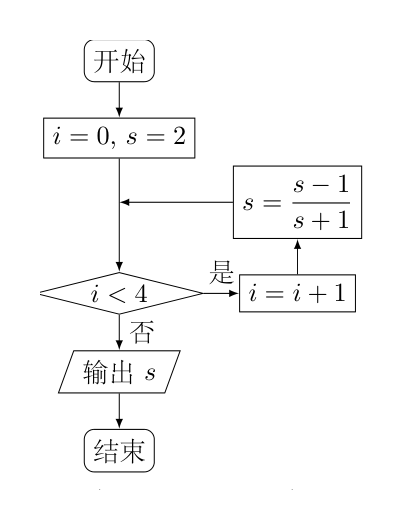
\includegraphics[width=0.65\linewidth]{GaoKao/images/2011/beijing_science/q4_fig1.png}
\end{center}

        {\centering\begin{tabular*}{\linewidth}{@{}@{\extracolsep{\fill}}llll@{}}
          \text{A. }\(-3\)  &  \text{B. }\(\frac{1}{2}\)  &  \text{C. }\(\frac{1}{3}\)  &  \text{D. }\(2\)
        \end{tabular*}\par}

        \item 如图，\(AD\)，\(AE\)，\(BC\) 分别与圆 \(O\) 切于点 \(D\)，\(E\)，\(F\)，延长 \(AF\) 与圆 \(O\) 交于另一点 \(G\). 给出下列三个结论：

\begin{enumerate}
\item \(AD + AE = AB + BC + CA\)；
\item \(AF \cdot AG = AD \cdot AE\)；
\item \(\triangle AFB \sim \triangle ADG\).
\end{enumerate}

其中正确结论的序号是（\quad）

\begin{center}
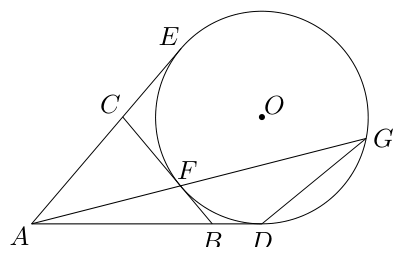
\includegraphics[width=10.0cm]{GaoKao/images/2011/beijing_science/q5_fig1.png}
\end{center}

        {\centering\begin{tabular*}{\linewidth}{@{}@{\extracolsep{\fill}}llll@{}}
          \text{A. }\(\ding{172}\ding{173}\)  &  \text{B. }\(\ding{173}\ding{174}\)  &  \text{C. }\(\ding{172}\ding{174}\)  &  \text{D. }\(\ding{172}\ding{173}\ding{174}\)
        \end{tabular*}\par}

        \item 根据统计，一名工人组装第 \(x\) 件某产品所用的时间（单位：分钟）为
\(f(x) = \begin{cases}
\dfrac{c}{\sqrt{x}}, & x < A,\\
\dfrac{c}{\sqrt{A}}, & x \geqslant A,
\end{cases}\)
（\(A\)，\(c\) 为常数）. 已知工人组装第 \(4\) 件产品用时 \(30\) 分钟，组装第 \(A\) 件产品用时 \(15\) 分钟，那么 \(c\) 和 \(A\) 的值分别是（\quad）

        {\centering\begin{tabular*}{\linewidth}{@{}@{\extracolsep{\fill}}llll@{}}
          \text{A. }\((75, 25)\)  &  \text{B. }\((75, 16)\)  &  \text{C. }\((60, 25)\)  &  \text{D. }\((60, 16)\)
        \end{tabular*}\par}

        \item 某四面体的三视图如图所示，该四面体四个面的面积中最大的是（\quad）

\begin{center}
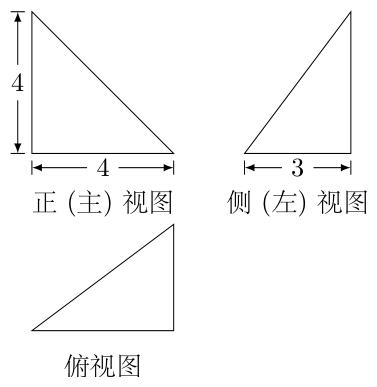
\includegraphics[width=6.2cm]{GaoKao/images/2011/beijing_science/q7_fig1.png}
\end{center}

        {\centering\begin{tabular*}{\linewidth}{@{}@{\extracolsep{\fill}}llll@{}}
          \text{A. }\(8\)  &  \text{B. }\(6\sqrt{2}\)  &  \text{C. }\(10\)  &  \text{D. }\(8\sqrt{2}\)
        \end{tabular*}\par}

        \item 设 \(A(0, 0)\)，\(B(4, 0)\)，\(C(t + 4, 4)\)，\(D(t, 4)\)（\(t \in \mathbb{R}\)）. 记 \(N(t)\) 为平行四边形 \(ABCD\) 内部（不含边界）的整点的个数，其中整点是指横，纵坐标都是整数的点，则函数 \(N(t)\) 的值域为（\quad）

        {\centering\begin{tabular*}{\linewidth}{@{}@{\extracolsep{\fill}}llll@{}}
          \text{A. }\(\{9, 10, 11\}\)  &  \text{B. }\(\{9, 10, 12\}\)  &  \text{C. }\(\{9, 11, 12\}\)  &  \text{D. }\(\{10, 11, 12\}\)
        \end{tabular*}\par}

    \end{enumerate}

\end{description}

\begin{description}

    \item[二、填空题]

    \begin{enumerate}[leftmargin=5pt]

      \addtocounter{enumi}{+8}

        \item 在 \(\triangle ABC\) 中，若 \(b = 5\)，\(\angle B = \frac{\pi}{4}\)，\(\tan A = 2\)，则 \(\sin A=\)\rule[-0.3ex]{3em}{0.4pt}；\(a=\)\rule[-0.3ex]{3em}{0.4pt}.

        \item 已知向量 \(\bm{a} = (\sqrt{3}, 1)\)，\(\bm{b} = (0, -1)\)，\(\bm{c} = (k, \sqrt{3})\). 若 \(\bm{a} - 2\bm{b}\) 与 \(\bm{c}\) 共线，则 \(k=\)\rule[-0.3ex]{3em}{0.4pt}.

        \item 在等比数列 \(\{a_n\}\) 中，\(a_1 = \frac{1}{2}\)，\(a_4 = -4\)，则公比 \(q=\)\rule[-0.3ex]{3em}{0.4pt}；\(|a_1| + |a_2| + \cdots + |a_n| = \)\rule[-0.3ex]{3em}{0.4pt}.

        \item 用数字 \(2\)，\(3\) 组成四位数，且数字 \(2\)，\(3\) 至少都出现一次，这样的四位数共有\rule[-0.3ex]{3em}{0.4pt} 个（用数字作答）.

        \item 已知函数 \(f(x) = \begin{cases}
\dfrac{2}{x}, & x \geqslant 2,\\
(x - 1)^3, & x < 2,
\end{cases}\)
若关于 \(x\) 的方程 \(f(x) = k\) 有两个不同的实根，则实数 \(k\) 的取值范围是\rule[-0.3ex]{3em}{0.4pt}.

        \item 曲线 \(C\) 是平面内与两个定点 \(F_1(-1, 0)\) 和 \(F_2(1, 0)\) 的距离的积等于常数 \(a^2\)（\(a > 1\)）的点的轨迹. 给出下列三个结论：

\begin{enumerate}
\item 曲线 \(C\) 过坐标原点；
\item 曲线 \(C\) 关于坐标原点对称；
\item 若点 \(P\) 在曲线 \(C\) 上，则 \(\triangle F_1PF_2\) 的面积不大于 \(\frac{1}{2}a^2\).
\end{enumerate}

其中所有正确结论的序号是\rule[-0.3ex]{3em}{0.4pt}.

    \end{enumerate}

\end{description}

\begin{description}

    \item[三、解答题]

    \begin{enumerate}[leftmargin=5pt]

      \addtocounter{enumi}{+14}

        \item 已知函数 \(f(x) = 4\cos x\sin \left(x + \frac{\pi}{6}\right) - 1\).

\begin{enumerate}
\item 求 \(f(x)\) 的最小正周期；
\item 求 \(f(x)\) 在区间 \(\left[-\frac{\pi}{6}, \frac{\pi}{4}\right]\) 上的最大值和最小值.
\end{enumerate}

        \item 如图，在四棱锥 \(P - ABCD\) 中，\(PA \perp\) 平面 \(ABCD\)，底面 \(ABCD\) 是菱形，\(AB = 2\)，\(\angle BAD = 60^{\circ}\).

\begin{enumerate}
\item 求证：\(BD \perp\) 平面 \(PAC\)；
\item 若 \(PA = AB\)，求 \(PB\) 与 \(AC\) 所成角的余弦值；
\item 当平面 \(PBC\) 与平面 \(PDC\) 垂直时，求 \(PA\) 的长.
\end{enumerate}

\begin{center}
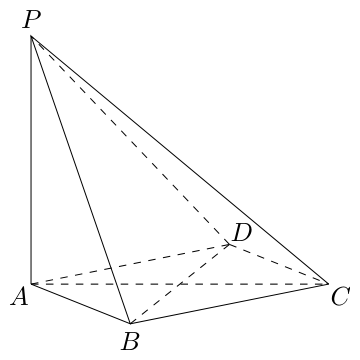
\includegraphics[width=9.7cm]{GaoKao/images/2011/beijing_science/q16_fig1.png}
\end{center}

        \item 以下茎叶图记录了甲，乙两组各四名同学的植树棵数. 乙组记录中有一个数据模糊，无法确认，在图中以 \(X\) 表示.

\begin{center}
\begin{tabular}{c|c|c}
甲组 & 茎 & 乙组 \\
\hline
\(9\quad 9\) & \(0\) & \(X\quad 8\quad 9\) \\
\(1\quad 1\) & \(1\) & \(0\)
\end{tabular}
\end{center}

\begin{enumerate}
\item 如果 \(X = 8\)，求乙组同学植树棵数的平均数和方差；
\item 如果 \(X = 9\)，分别从甲，乙两组中随机选取一名同学，求这两名同学的植树总棵数 \(Y\) 的分布列和数学期望.
\end{enumerate}

（注：方差 \(s^2 = \frac{1}{n}\left[(x_1 - \bar{x})^2 + (x_2 - \bar{x})^2 + \cdots + (x_n - \bar{x})^2\right]\)，其中 \(\bar{x}\) 为 \(x_1\)，\(x_2\)，\(\cdots\)，\(x_n\) 的平均数）

        \item 已知函数 \(f(x) = (x - k)^2{\mathrm{e}}^{\frac{x}{k}}\).

\begin{enumerate}
\item 求 \(f(x)\) 的单调区间；
\item 若对于任意的 \(x \in (0, +\infty)\)，都有 \(f(x) \leqslant \frac{1}{{\mathrm{e}}}\)，求 \(k\) 的取值范围.
\end{enumerate}

        \item 已知椭圆 \(G: \frac{x^2}{4} + y^2 = 1\). 过点 \((m, 0)\) 作圆 \(x^2 + y^2 = 1\) 的切线 \(l\)，交椭圆 \(G\) 于 \(A\)，\(B\) 两点.

\begin{enumerate}
\item 求椭圆 \(G\) 的焦点坐标和离心率；
\item 将 \(\left|AB\right|\) 表示为 \(m\) 的函数，并求 \(\left|AB\right|\) 的最大值.
\end{enumerate}

        \item 若数列 \(A_n : a_1\)，\(a_2\)，\(\cdots\)，\(a_n\)（\(n \geqslant 2\)）满足 \(\left|a_{k+1} - a_k\right| = 1\)（\(k = 1\)，\(2\)，\(\cdots\)，\(n - 1\)），则称 \(A_n\) 为 \(E\) 数列. 记 \(S(A_n) = a_1 + a_2 + \cdots + a_n\).

\begin{enumerate}
\item 写出一个满足 \(a_1 = a_5 = 0\)，且 \(S(A_5) > 0\) 的 \(E\) 数列 \(A_5\)；
\item 若 \(a_1 = 12\)，\(n = 2000\)，证明：\(E\) 数列 \(A_n\) 是递增数列的充要条件是 \(a_n = 2011\)；
\item 对任意给定的整数 \(n\)（\(n \geqslant 2\)），是否存在首项为 \(0\) 的 \(E\) 数列 \(A_n\)，使得 \(S(A_n) = 0\)？如果存在，写出一个满足条件的 \(E\) 数列 \(A_n\)；如果不存在，说明理由.
\end{enumerate}

    \end{enumerate}

\end{description}


\subsection{2011年北京卷（文）}\label{gk:2011年北京卷（文）}

\begin{description}

    \item[一、选择题]

    \begin{enumerate}[leftmargin=5pt]

        \item 已知全集 \(U = \mathbb{R}\)，集合 \(P = \{x \mid x^2 \leqslant 1\}\)，那么 \(\complement_U P =\)（\quad）

        {\centering\begin{tabular*}{\linewidth}{@{}@{\extracolsep{\fill}}llll@{}}
          \text{A. }\((-\infty, -1]\)  &  \text{B. }\([1, +\infty)\)  &  \text{C. }\((-1, 1)\)  &  \text{D. }\((-\infty, -1) \cup (1, +\infty)\)
        \end{tabular*}\par}

        \item 复数 \(\frac{\i - 2}{1 + 2\i} =\)（\quad）

        {\centering\begin{tabular*}{\linewidth}{@{}@{\extracolsep{\fill}}llll@{}}
          \text{A. }\(\i\)  &  \text{B. }\(-\i\)  &  \text{C. }\(-\frac{4}{5} - \frac{3}{5}\i\)  &  \text{D. }\(-\frac{4}{5} + \frac{3}{5}\i\)
        \end{tabular*}\par}

        \item 如果 \(\log_{\frac{1}{2}} x < \log_{\frac{1}{2}} y < 0\)，那么（\quad）

        {\centering\begin{tabular*}{\linewidth}{@{}@{\extracolsep{\fill}}llll@{}}
          \text{A. }\(y < x < 1\)  &  \text{B. }\(x < y < 1\)  &  \text{C. }\(1 < x < y\)  &  \text{D. }\(1 < y < x\)
        \end{tabular*}\par}

        \item 若 \(p\) 是真命题，\(q\) 是假命题，则（\quad）

        {\centering\begin{tabular*}{\linewidth}{@{}@{\extracolsep{\fill}}llll@{}}
          \text{A. }\(p \wedge q\) 是真命题  &  \text{B. }\(p \vee q\) 是假命题  &  \text{C. }\(\neg p\) 是真命题  &  \text{D. }\(\neg q\) 是真命题
        \end{tabular*}\par}

        \item 某四棱锥的三视图如图所示，该四棱锥的表面积是（\quad）

\begin{center}
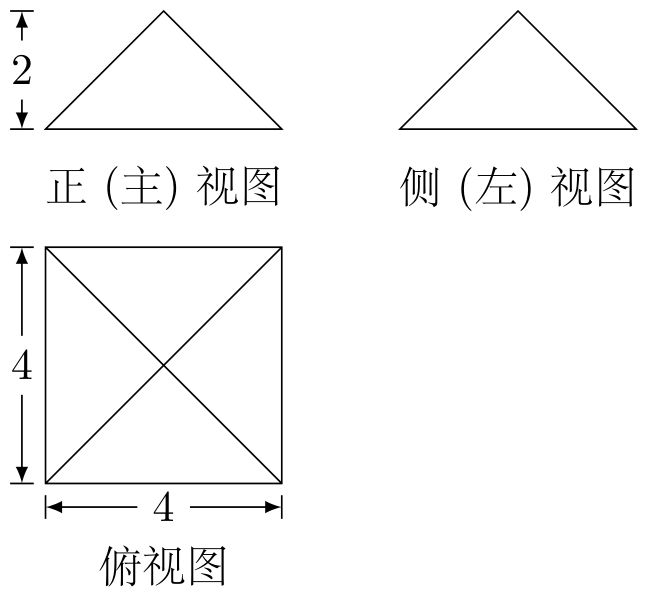
\includegraphics[width=6.3cm]{GaoKao/images/2011/beijing_liberal/q5_fig1.png}
\end{center}

        {\centering\begin{tabular*}{\linewidth}{@{}@{\extracolsep{\fill}}llll@{}}
          \text{A. }\(32\)  &  \text{B. }\(16 + 16\sqrt{2}\)  &  \text{C. }\(48\)  &  \text{D. }\(16 + 32\sqrt{2}\)
        \end{tabular*}\par}

        \item 执行如图所示的程序框图，若输入 \(A\) 的值为 2，则输出的 \(P\) 的值为（\quad）

\begin{center}
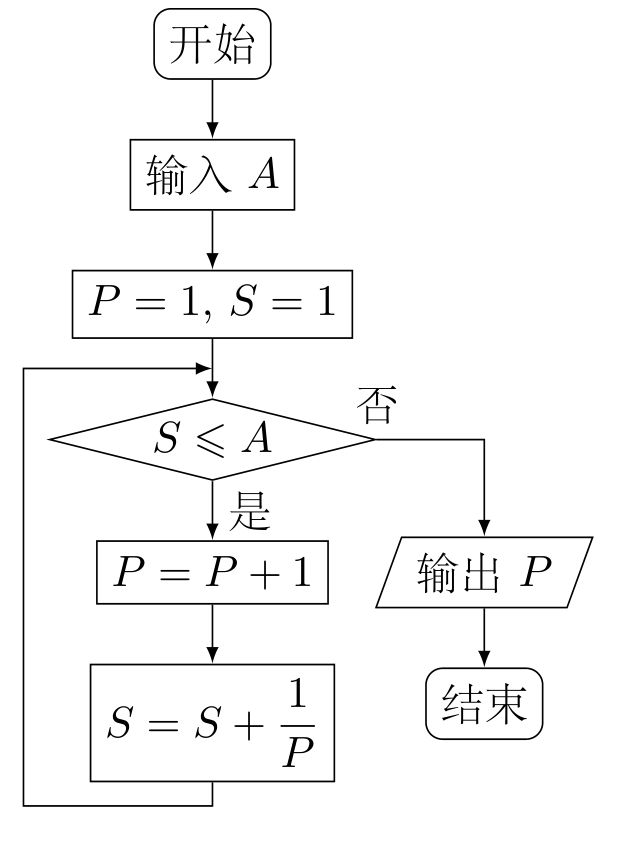
\includegraphics[width=0.38\linewidth]{GaoKao/images/2011/beijing_liberal/q6_fig1.png}
\end{center}

        {\centering\begin{tabular*}{\linewidth}{@{}@{\extracolsep{\fill}}llll@{}}
          \text{A. }\(2\)  &  \text{B. }\(3\)  &  \text{C. }\(4\)  &  \text{D. }\(5\)
        \end{tabular*}\par}

        \item 某车间分批生产某种产品，每批的生产准备费用为 \(800\text{ 元}\). 若每批生产 \(x\) 件，则平均仓储时间为 \(\frac{x}{8}\text{ 天}\)，且每件产品每天的仓储费用为 \(1\text{ 元}\). 为使平均到每件产品的生产准备费用与仓储费用之和最小，每批应生产产品（\quad）

        {\centering\begin{tabular*}{\linewidth}{@{}@{\extracolsep{\fill}}llll@{}}
          \text{A. }\(60\text{ 件}\)  &  \text{B. }\(80\text{ 件}\)  &  \text{C. }\(100\text{ 件}\)  &  \text{D. }\(120\text{ 件}\)
        \end{tabular*}\par}

        \item 已知点 \(A(0,2)\)，\(B(2,0)\). 若点 \(C\) 在函数 \(y = x^2\) 的图象上，则使得 \(\triangle ABC\) 的面积为 2 的点 \(C\) 的个数为（\quad）

        {\centering\begin{tabular*}{\linewidth}{@{}@{\extracolsep{\fill}}llll@{}}
          \text{A. }\(4\)  &  \text{B. }\(3\)  &  \text{C. }\(2\)  &  \text{D. }\(1\)
        \end{tabular*}\par}

    \end{enumerate}

\end{description}

\begin{description}

    \item[二、填空题]

    \begin{enumerate}[leftmargin=5pt]

      \addtocounter{enumi}{+8}

        \item 在 \(\triangle ABC\) 中，若 \(b = 5\)，\(\angle B = \frac{\pi}{4}\)，\(\sin A = \frac{1}{3}\)，则 \(a =\)\rule[-0.3ex]{3em}{0.4pt}.

        \item 已知双曲线 \(x^{2}-\frac{y^{2}}{b^{2}}=1\)（\(b>0\)）的一条渐近线的方程为 \(y = 2x\)，则 \(b=\)\rule[-0.3ex]{3em}{0.4pt}.

        \item 已知向量 \(\bm{a} = (\sqrt{3}, 1)\)，\(\bm{b} = (0, -1)\)，\(\bm{c} = (k, \sqrt{3})\). 若 \(\bm{a} - 2\bm{b}\) 与 \(\bm{c}\) 共线，则 \(k =\)\rule[-0.3ex]{3em}{0.4pt}.

        \item 在等比数列 \(\left\{a_{n}\right\}\) 中，\(a_{1}=\frac{1}{2}\)，\(a_{4}=-4\)，则公比 \(q=\)\rule[-0.3ex]{3em}{0.4pt}；\(a_{1}+a_{2}+\cdots+a_{n}=\)\rule[-0.3ex]{3em}{0.4pt}.

        \item 已知函数 \(f(x) = \begin{cases}
\dfrac{2}{x}, & x \geqslant 2,\\
(x - 1)^3, & x < 2,
\end{cases}\)
若关于 \(x\) 的方程 \(f(x) = k\) 有两个不同的实根，则实数 \(k\) 的取值范围是\rule[-0.3ex]{3em}{0.4pt}.

        \item 设 \(A(0,0)\)，\(B(4,0)\)，\(C(t + 4,3)\)，\(D(t,3) \)（\(t \in \mathbb{R}\)）. 记 \(N(t)\) 为平行四边形 \(ABCD\) 内部（不含边界）的整点的个数. 其中整点是指横，纵坐标都是整数的点，则 \(N(0) =\)\rule[-0.3ex]{3em}{0.4pt}；\(N(t)\) 的所有可能取值为\rule[-0.3ex]{3em}{0.4pt}.

    \end{enumerate}

\end{description}

\begin{description}

    \item[三、解答题]

    \begin{enumerate}[leftmargin=5pt]

      \addtocounter{enumi}{+14}

        \item 已知函数 \( f(x) = 4\cos x\sin \left(x + \frac{\pi}{6}\right) - 1 \).
\begin{enumerate}
\item 求 \( f(x) \) 的最小正周期.
\item 求 \( f(x) \) 在区间 \( \left[-\frac{\pi}{6}, \frac{\pi}{4}\right] \) 上的最大值和最小值.
\end{enumerate}

        \item 以下茎叶图记录了甲，乙两组各四名同学的植树棵数. 乙组记录中有一个数据模糊，无法确认，在图中以 \(X\) 表示.

\begin{center}
\begin{tabular}{r|c|l}
甲组 & & 乙组 \\
\hline
\(9\quad 9\) & 0 & \(X\quad 8\quad 9\) \\
\(1\quad 1\) & 1 & \(0\)
\end{tabular}
\end{center}

\begin{enumerate}
\item 如果 \(X = 8\)，求乙组同学植树棵数的平均数和方差；
\item 如果 \(X = 9\)，分别从甲，乙两组中随机选取一名同学，求这两名同学的植树总棵数为 19 的概率.
\end{enumerate}
（注：方差 \( s^2 = \frac{1}{n}\left[(x_1 - \overline{x})^2 + (x_2 - \overline{x})^2 + \ldots + (x_n - \overline{x})^2\right] \)，其中 \(\overline{x}\) 为 \(x_1\)，\(x_2\)，\(\cdots\)，\(x_n\) 的平均数）

        \item 如图，在四面体 \(PABC\) 中，\(PC \perp AB\)，\(PA \perp BC\)，点 \(D\)，\(E\)，\(F\)，\(G\) 分别是棱 \(AP\)，\(AC\)，\(BC\)，\(PB\) 的中点.

\begin{enumerate}
\item 求证：\(DE \parallel\) 平面 \(BCP\)；
\item 求证：四边形 \(DEFG\) 为矩形；
\item 是否存在点 \(Q\)，到四面体 \(PABC\) 六条棱的中点的距离相等？说明理由.
\end{enumerate}

\begin{center}
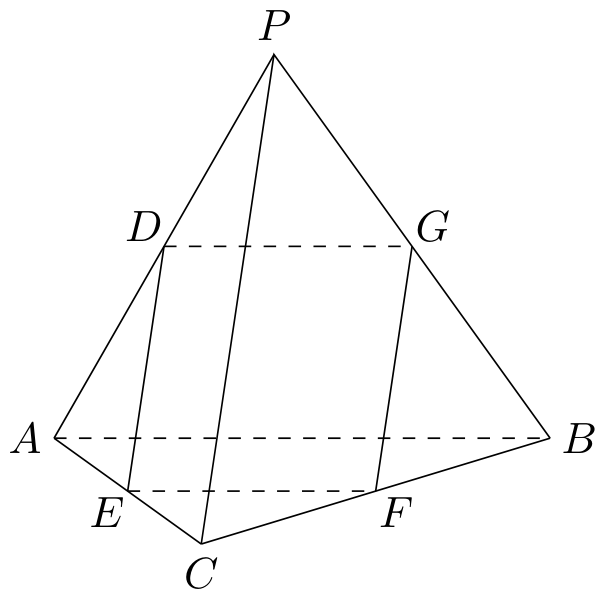
\includegraphics[width=7.5cm]{GaoKao/images/2011/beijing_liberal/q17_fig1.png}
\end{center}

        \item 已知函数 \( f(x) = (x - k){\mathrm{e}}^x \).
\begin{enumerate}
\item 求 \( f(x) \) 的单调区间；
\item 求 \( f(x) \) 在区间 \( [0,1] \) 上的最小值.
\end{enumerate}

        \item 已知椭圆 \(G: \frac{x^2}{a^{2}} + \frac{y^2}{b^{2}} = 1 \) （\(a > b > 0\)）的离心率为 \(\frac{\sqrt{6}}{3}\)，右焦点为 \((2\sqrt{2}, 0)\)，斜率为 1 的直线 \(l\) 与椭圆 \(G\) 交于 \(A\)，\(B\) 两点. 以 \(AB\) 为底边作等腰三角形，顶点为 \(P(-3, 2)\).
\begin{enumerate}
\item 求椭圆 \(G\) 的方程；
\item 求 \( \triangle PAB \) 的面积.
\end{enumerate}

        \item 若数列 \(A_{n}\)：\(a_{1}\)，\(a_{2}\)，\(\cdots\)，\(a_{n}\)（\(n \geqslant 2\)）满足 \(\left|a_{k+1} - a_{k}\right| = 1\)（\(k = 1, 2, \cdots, n-1\)），则称 \(A_{n}\) 为 \(E\) 数列. 记 \(S(A_{n}) = a_{1} + a_{2} + \cdots + a_{n}\).
\begin{enumerate}
\item 写出一个 \(E\) 数列 \(A_{n}\) 满足 \(a_{1}=a_{3}=0\)；
\item 若 \(a_1 = 12\)，\(n = 2000\)，证明：\(E\) 数列 \(A_n\) 是递增数列的充要条件是 \(a_n = 2011\)；
\item 在 \(a_1 = 4\) 的 \(E\) 数列 \(A_n\) 中，求使得 \(S(A_n) = 0\) 成立的 \(n\) 的最小值.
\end{enumerate}

    \end{enumerate}

\end{description}


\subsection{2011年重庆卷（理）}\label{gk:2011年重庆卷（理）}

\begin{description}

    \item[一、选择题]

    \begin{enumerate}[leftmargin=5pt]

        \item 复数 \(\frac{\i^2 + \i^3 + \i^4}{1 - \i} =\)（\quad）

        {\centering\begin{tabular*}{\linewidth}{@{}@{\extracolsep{\fill}}llll@{}}
          \text{A. }\(-\frac{1}{2} - \frac{1}{2}\i\)  &  \text{B. }\(-\frac{1}{2} + \frac{1}{2}\i\)  &  \text{C. }\(\frac{1}{2} - \frac{1}{2}\i\)  &  \text{D. }\(\frac{1}{2} + \frac{1}{2}\i\)
        \end{tabular*}\par}

        \item “\(x < -1\)”是“ \( x^{2} - 1 > 0 \) ”的（\quad）

        {\centering\begin{tabular*}{\linewidth}{@{}@{\extracolsep{\fill}}llll@{}}
          \text{A. }充分而不必要条件  &  \text{B. }必要而不充分条件  &  \text{C. }充要条件  &  \text{D. }既不充分也不必要条件
        \end{tabular*}\par}

        \item 已知 \(\lim\limits_{x\to +\infty}\left(\frac{2}{x - 1} + \frac{ax - 1}{3x}\right) = 2\)，则 \(a =\)（\quad）

        {\centering\begin{tabular*}{\linewidth}{@{}@{\extracolsep{\fill}}llll@{}}
          \text{A. }\(-6\)  &  \text{B. }2  &  \text{C. }3  &  \text{D. }6
        \end{tabular*}\par}

        \item \((1 + 3x)^{n}\) （其中 \(n\in \mathbb{N}\) 且 \(n\geqslant 6\) ）的展开式中 \(x^{5}\) 与 \(x^{6}\) 的系数相等，则（\quad）

        {\centering\begin{tabular*}{\linewidth}{@{}@{\extracolsep{\fill}}llll@{}}
          \text{A. }6  &  \text{B. }7  &  \text{C. }8  &  \text{D. }9
        \end{tabular*}\par}

        \item 下列区间中，函数 \( f(x) = |\ln (2 - x)| \) 在其上为增函数的是（\quad）

        {\centering\begin{tabular*}{\linewidth}{@{}@{\extracolsep{\fill}}llll@{}}
          \text{A. }\((-\infty, 1]\)  &  \text{B. }\(\left[-1, \frac{4}{3}\right]\)  &  \text{C. }\(\left[0, \frac{3}{2}\right)\)  &  \text{D. }\([1,2)\)
        \end{tabular*}\par}

        \item 若 \(\triangle ABC\) 的内角 \(A\)，\(B\)，\(C\) 所对的边 \(a\)，\(b\)，\(c\) 满足 \((a + b)^2 - c^2 = 4\)，且 \(C = 60^\circ\)，则 \(ab\) 的值为（\quad）

        {\centering\begin{tabular*}{\linewidth}{@{}@{\extracolsep{\fill}}llll@{}}
          \text{A. }\( \frac{4}{3} \)  &  \text{B. }\(8 - 4\sqrt{3}\)  &  \text{C. }1  &  \text{D. }\( \frac{2}{3} \)
        \end{tabular*}\par}

        \item 已知 \(a > 0\)，\(b > 0\)，\(a + b = 2\)，则 \(y = \frac{1}{a} + \frac{4}{b}\) 的最小值是（\quad）

        {\centering\begin{tabular*}{\linewidth}{@{}@{\extracolsep{\fill}}llll@{}}
          \text{A. }\( \frac{7}{2} \)  &  \text{B. }4  &  \text{C. }\( \frac{9}{2} \)  &  \text{D. }5
        \end{tabular*}\par}

        \item 在圆 \(x^{2} + y^{2} - 2x - 6y = 0\) 内，过点 \(E(0,1)\) 的最长弦和最短弦分别为 \(AC\) 和 \(BD\)，则四边形 \(ABCD\) 的面积为（\quad）

        {\centering\begin{tabular*}{\linewidth}{@{}@{\extracolsep{\fill}}llll@{}}
          \text{A. }\( 5\sqrt{2} \)  &  \text{B. }\(10\sqrt{2}\)  &  \text{C. }\(15\sqrt{2}\)  &  \text{D. }\(20\sqrt{2}\)
        \end{tabular*}\par}

        \item 高为 \(\frac{\sqrt{2}}{4}\) 的四棱锥 \(S - ABCD\) 的底面是边长为 1 的正方形，点 \(S\)，\(A\)，\(B\)，\(C\)，\(D\) 均在半径为 1 的同一球面上，则底面 \(ABCD\) 的中心与顶点 \(S\) 之间的距离为（\quad）

        {\centering\begin{tabular*}{\linewidth}{@{}@{\extracolsep{\fill}}llll@{}}
          \text{A. }\( \frac{\sqrt{2}}{4} \)  &  \text{B. }\( \frac{\sqrt{2}}{2} \)  &  \text{C. }1  &  \text{D. }\(\sqrt{2}\)
        \end{tabular*}\par}

        \item 设 \(m\)，\(k\) 为整数，方程 \(mx^2 - kx + 2 = 0\) 在区间 \((0,1)\) 内有两个不同的根，则 \(m + k\) 的最小值为（\quad）

        {\centering\begin{tabular*}{\linewidth}{@{}@{\extracolsep{\fill}}llll@{}}
          \text{A. }\(-8\)  &  \text{B. }8  &  \text{C. }12  &  \text{D. }13
        \end{tabular*}\par}

    \end{enumerate}

\end{description}

\begin{description}

    \item[二、填空题]

    \begin{enumerate}[leftmargin=5pt]

      \addtocounter{enumi}{+10}

        \item 在等差数列 \(\{a_{n}\}\) 中，\(a_{3} + a_{7} = 37\)，则 \(a_{2} + a_{4} + a_{6} + a_{8} =\rule[-0.3ex]{3em}{0.4pt}\).

        \item 已知单位向量 \(e_1\)，\(e_2\) 的夹角为 \(60^\circ\)，则 \(|2e_1 - e_2| =\rule[-0.3ex]{3em}{0.4pt}\).

        \item 将一枚均匀的硬币抛掷 6 次，则正面出现的次数比反面出现的次数多的概率为\rule[-0.3ex]{3em}{0.4pt}.

        \item 已知 \(\sin \alpha = \frac{1}{2} + \cos \alpha\)，且 \(\alpha \in \left(0, \frac{\pi}{2}\right)\)，则 \(\frac{\cos 2\alpha}{\sin \left(\alpha - \frac{\pi}{4}\right)}\) 的值为\rule[-0.3ex]{3em}{0.4pt}.

        \item 设圆 \(C\) 位于抛物线 \(y^{2} = 2x\) 与直线 \(x = 3\) 所围成的封闭区域（包含边界）内，则圆 \(C\) 的半径能取到的最大值为\rule[-0.3ex]{3em}{0.4pt}.

    \end{enumerate}

\end{description}

\begin{description}

    \item[三、解答题]

    \begin{enumerate}[leftmargin=5pt]

      \addtocounter{enumi}{+15}

        \item 设 \(a \in \mathbb{R}\)，\(f(x) = \cos x (a \sin x - \cos x) + \cos^2 \left(\frac{\pi}{2} - x\right)\) 满足 \(f\left(-\frac{\pi}{3}\right) = f(0)\)，求函数 \(f(x)\) 在 \(\left[\frac{\pi}{4}, \frac{11\pi}{24}\right]\) 上的最大值和最小值.

        \item 某市公租房的房源位于 \(A\)，\(B\)，\(C\) 三个片区. 设每位申请人只申请其中一个片区的房源. 且申请其中任一个片区的房源是等可能的. 求该市的任 \(4\) 位申请人中：
\begin{enumerate}
\item 恰有 2 人申请 \(A\) 片区的房源的概率；
\item 申请的房源所在片区的个数 \(\xi\) 的分布列与期望.
\end{enumerate}

        \item 设 \( f(x) = x^3 + ax^2 + bx + 1 \) 的导数 \( f'(x) \) 满足 \( f'(1) = 2a \)，\( f'(2) = -b \)，其中常数 \(a\)，\(b \in \mathbb{R}\).
\begin{enumerate}
\item 求曲线 \( y = f(x) \) 在点 \((1, f(1))\) 处的切线方程；
\item 设 \( g(x) = f'(x) {\mathrm{e}}^{-x} \)，求函数 \( g(x) \) 的极值.
\end{enumerate}

        \item 如图，在四面体 \(ABCD\) 中，平面 \(ABC \perp\) 平面 \(ACD\)，\(AB \perp BC\)，\(AD = CD\)，\(\angle CAD = 30^\circ\).
\begin{enumerate}
\item 若 \(AD = 2\)，\(AB = 2BC\)，求四面体 \(ABCD\) 的体积；
\item 若二面角 \(C - AB - D\) 为 \(60^{\circ}\)，求异面直线 \(AD\) 与 \(BC\) 所成角的余弦值.
\end{enumerate}

\begin{center}
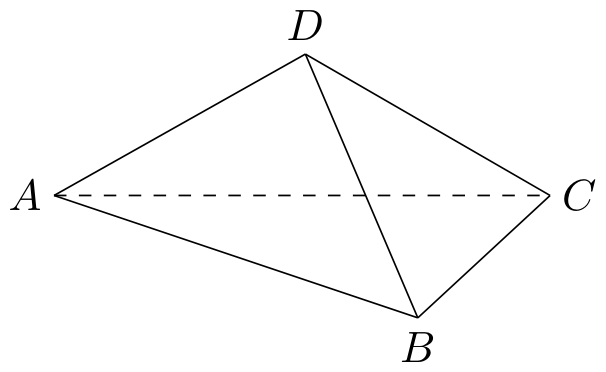
\includegraphics[width=7.5cm]{GaoKao/images/2011/chongqing_science/q19_fig1.png}
\end{center}

        \item 如图，椭圆的中心为原点 \(O\)，离心率 \(e = \frac{\sqrt{2}}{2}\)，一条准线的方程为 \(x = 2\sqrt{2}\).
\begin{enumerate}
\item 求该椭圆的标准方程；
\item 设动点 \(P\) 满足： \(\overrightarrow{OP} = \overrightarrow{OM} + 2\overrightarrow{ON}\)，其中 \(M\)，\(N\) 是椭圆上的点，直线 \(OM\) 与 \(ON\) 的斜率之积为 \(-\frac{1}{2}\). 问：是否存在两个定点 \(F_1\)，\(F_2\)，使得 \(|PF_1| + |PF_2|\) 为定值？若存在，求 \(F_1\)，\(F_2\) 的坐标；若不存在，说明理由.
\end{enumerate}

\begin{center}
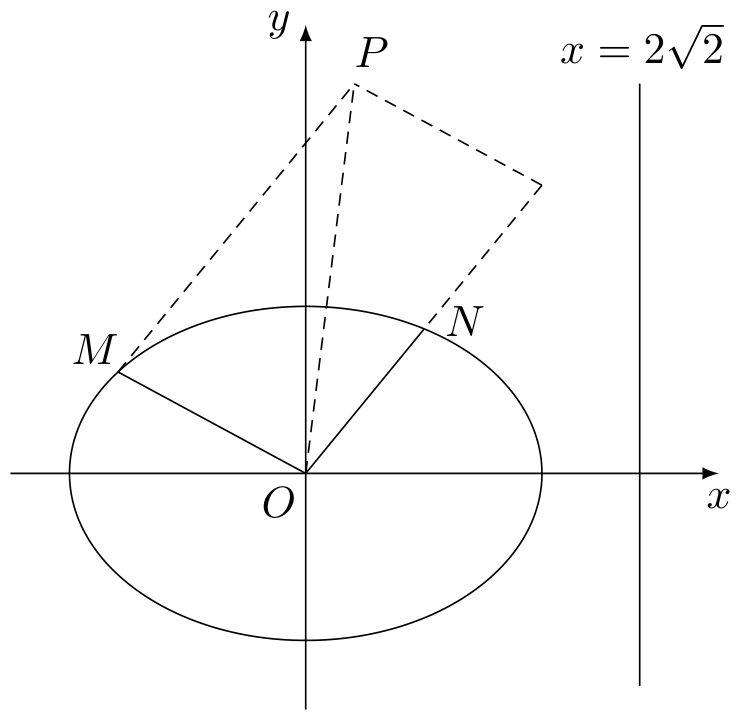
\includegraphics[width=8.9cm]{GaoKao/images/2011/chongqing_science/q20_fig1.png}
\end{center}

        \item 设实数数列 \(\{a_{n}\}\) 的前 \(n\) 项和 \(S_{n}\) 满足 \(S_{n + 1} = a_{n + 1}S_n\) （\(n\in \mathbb{N}^*\)）.
\begin{enumerate}
\item 若 \(a_{1}\)，\(S_{2}\)，\(-2a_{2}\) 成等比数列，求 \(S_{2}\) 和 \(a_{3}\)；
\item 求证：对 \(k \geqslant 3\) 有 \(0 \leqslant a_{k+1} \leqslant a_k \leqslant \frac{4}{3}\).
\end{enumerate}

    \end{enumerate}

\end{description}


\subsection{2011年重庆卷（文）}\label{gk:2011年重庆卷（文）}

\begin{description}

    \item[一、选择题]

    \begin{enumerate}[leftmargin=5pt]

        \item 在等差数列 \(\{a_{n}\}\) 中，\(a_{2} = 2\)，\(a_{3} = 4\)，则 \(a_{10} =\)（\quad）

        {\centering\begin{tabular*}{\linewidth}{@{}@{\extracolsep{\fill}}llll@{}}
          \text{A. }\(12\)  &  \text{B. }\(14\)  &  \text{C. }\(16\)  &  \text{D. }\(18\)
        \end{tabular*}\par}

        \item 设 \(U = \mathbb{R}\)，\(M = \{x \mid x^2 - 2x > 0\}\)，则 \(\complement_U M =\)（\quad）

        {\centering\begin{tabular*}{\linewidth}{@{}@{\extracolsep{\fill}}llll@{}}
          \text{A. }\(\left[0,2\right]\)  &  \text{B. }\(\left(0,2\right)\)  &  \text{C. }\(\left(-\infty,0\right)\cup\left(2,+\infty\right)\)  &  \text{D. }\(\left(-\infty,0\right]\cup\left[2,+\infty\right)\)
        \end{tabular*}\par}

        \item 曲线 \( y = -x^{3} + 3x^{2} \) 在点\(\left(1,2\right)\)处的切线方程为（\quad）

        {\centering\begin{tabular*}{\linewidth}{@{}@{\extracolsep{\fill}}llll@{}}
          \text{A. }\(y = 3x - 1\)  &  \text{B. }\(y = -3x + 5\)  &  \text{C. }\(y = 3x + 5\)  &  \text{D. }\(y = 2x\)
        \end{tabular*}\par}

        \item 从一堆苹果中任取 \(10\) 只，称得它们的质量如下（单位：\(\text{克}\)）：\(125\)，\(120\)，\(122\)，\(105\)，\(130\)，\(114\)，\(116\)，\(95\)，\(120\)，\(134\)，则样本数据落在 \(\left[114.5,124.5\right]\) 内的频率为（\quad）

        {\centering\begin{tabular*}{\linewidth}{@{}@{\extracolsep{\fill}}llll@{}}
          \text{A. }\(0.2\)  &  \text{B. }\(0.3\)  &  \text{C. }\(0.4\)  &  \text{D. }\(0.5\)
        \end{tabular*}\par}

        \item 已知向量 \(\bm{a} = (1, k)\)，\(\bm{b} = (2, 2)\)，且 \(\bm{a} + \bm{b}\) 与 \(\bm{a}\) 共线，那么 \(\bm{a} \cdot \bm{b}\) 的值为（\quad）

        {\centering\begin{tabular*}{\linewidth}{@{}@{\extracolsep{\fill}}llll@{}}
          \text{A. }\(1\)  &  \text{B. }\(2\)  &  \text{C. }\(3\)  &  \text{D. }\(4\)
        \end{tabular*}\par}

        \item 设 \(a = \log_{\frac{1}{3}} \frac{1}{2}\)，\(b = \log_{\frac{1}{3}} \frac{2}{3}\)，\(c = \log_3 \frac{4}{3}\)，则 \(a\)，\(b\)，\(c\) 的大小关系是（\quad）

        {\centering\begin{tabular*}{\linewidth}{@{}@{\extracolsep{\fill}}llll@{}}
          \text{A. }\(a < b < c\)  &  \text{B. }\(c < b < a\)  &  \text{C. }\(b < a < c\)  &  \text{D. }\(b < c < a\)
        \end{tabular*}\par}

        \item 若函数 \( f(x) = x + \frac{1}{x - 2} \)（\(x > 2\)）在 \( x = a \) 处取最小值，则 \( a = \)（\quad）

        {\centering\begin{tabular*}{\linewidth}{@{}@{\extracolsep{\fill}}llll@{}}
          \text{A. }\(1 + \sqrt{2}\)  &  \text{B. }\(1 + \sqrt{3}\)  &  \text{C. }\(3\)  &  \text{D. }\(4\)
        \end{tabular*}\par}

        \item 若 \(\triangle ABC\) 的内角 \(A\)，\(B\)，\(C\) 满足 \(6\sin A = 4\sin B = 3\sin C\)，则 \(\cos B =\)（\quad）

        {\centering\begin{tabular*}{\linewidth}{@{}@{\extracolsep{\fill}}llll@{}}
          \text{A. }\(\frac{\sqrt{15}}{4}\)  &  \text{B. }\(\frac{3}{4}\)  &  \text{C. }\(\frac{3\sqrt{15}}{16}\)  &  \text{D. }\(\frac{11}{16}\)
        \end{tabular*}\par}

        \item 设双曲线的左准线与两条渐近线交于 \(A\)，\(B\) 两点，左焦点在以 \(AB\) 为直径的圆内，则该双曲线的离心率取值范围为（\quad）

        {\centering\begin{tabular*}{\linewidth}{@{}@{\extracolsep{\fill}}llll@{}}
          \text{A. }\(\left(0,\sqrt{2}\right)\)  &  \text{B. }\(\left(1,\sqrt{2}\right)\)  &  \text{C. }\(\left(\frac{\sqrt{2}}{2}, 1\right)\)  &  \text{D. }\(\left(\sqrt{2},+\infty\right)\)
        \end{tabular*}\par}

        \item 高为 \(\sqrt{2}\) 的四棱锥 \(S - ABCD\) 的底面是边长为 \(1\) 的正方形，点 \(S\)，\(A\)，\(B\)，\(C\)，\(D\) 均在半径为 \(1\) 的同一球面上，则底面 \(ABCD\) 的中心与顶点 \(S\) 之间的距离为（\quad）

        {\centering\begin{tabular*}{\linewidth}{@{}@{\extracolsep{\fill}}llll@{}}
          \text{A. }\(\frac{\sqrt{10}}{2}\)  &  \text{B. }\(\frac{\sqrt{2} + \sqrt{3}}{2}\)  &  \text{C. }\(\frac{3}{2}\)  &  \text{D. }\(\sqrt{2}\)
        \end{tabular*}\par}

    \end{enumerate}

\end{description}

\begin{description}

    \item[二、填空题]

    \begin{enumerate}[leftmargin=5pt]

      \addtocounter{enumi}{+10}

        \item \(\left(1 + 2x\right)^{6}\) 的展开式中 \(x^{4}\) 的系数是\rule[-0.3ex]{3em}{0.4pt}.

        \item 若 \(\cos \alpha = -\frac{3}{5}\)，且 \(\alpha \in \left(\pi, \frac{3\pi}{2}\right)\)，则 \(\tan \alpha =\)\rule[-0.3ex]{3em}{0.4pt}.

        \item 过原点的直线与圆 \(x^{2} + y^{2} - 2x - 4y + 4 = 0\) 相交所得弦的长为\(2\)，则该直线的方程为\rule[-0.3ex]{3em}{0.4pt}.

        \item 从甲，乙等\(10\)位同学中任选\(3\)位去参加某项活动，则所选\(3\)位中有甲但没有乙的概率为\rule[-0.3ex]{3em}{0.4pt}.

        \item 若实数 \(a\)，\(b\)，\(c\) 满足 \(2^{a} + 2^{b} = 2^{a + b}\)，\(2^{a} + 2^{b} + 2^{c} = 2^{a + b + c}\)，则 \(c\) 的最大值是\rule[-0.3ex]{3em}{0.4pt}.

    \end{enumerate}

\end{description}

\begin{description}

    \item[三、解答题]

    \begin{enumerate}[leftmargin=5pt]

      \addtocounter{enumi}{+15}

        \item 设 \(\{a_{n}\}\) 是公比为正数的等比数列，\(a_{1} = 2\)，\(a_{3} = a_{2} + 4\).
\begin{enumerate}
\item 求 \( \{a_{n}\} \) 的通项公式；
\item 设 \( \{b_{n}\} \) 是首项为 1，公差为 2 的等差数列. 求数列 \( \{a_{n} + b_{n}\} \) 的前 \(n\) 项和 \(S_{n}\).
\end{enumerate}

        \item 某市公租房的房源位于 \(A\)，\(B\)，\(C\) 三个片区. 设每位申请人只申请其中一个片区的房源，且申请其中任一个片区的房源是等可能的，求该市的任 \(4\) 位申请人中：
\begin{enumerate}
\item 没有人申请 \(A\) 片区房源的概率；
\item 每个片区的房源都有人申请的概率.
\end{enumerate}

        \item 设函数 \(f(x) = \sin x \cos x - \sqrt{3}\cos\left(\pi + x\right)\cos x\) （\(x \in \mathbb{R}\)）.
\begin{enumerate}
\item 求 \(f(x)\) 的最小正周期；
\item 若函数 \(y = f(x)\) 的图象按 \(\bm{b} = \left(\frac{\pi}{4}, \frac{\sqrt{3}}{2}\right)\) 平移后得到函数 \(y = g(x)\) 的图象，求 \(y = g(x)\) 在 \(\left[0, \frac{\pi}{4}\right]\) 上的最大值.
\end{enumerate}

        \item 设 \( f(x) = 2x^{3} + ax^{2} + bx + 1 \) 的导数为 \( f'(x) \). 若函数 \( y = f'(x) \) 的图象关于直线 \( x = -\frac{1}{2} \) 对称，且 \( f'(1) = 0 \).
\begin{enumerate}
\item 求实数 \(a\)，\(b\) 的值；
\item 求函数 \( f(x) \) 的极值.
\end{enumerate}

        \item 如图，在四面体 \(ABCD\) 中，平面 \(ABC \perp\) 平面 \(ACD\)，\(AB \perp BC\)，\(AC = AD = 2\)，\(BC = CD = 1\).
\begin{enumerate}
\item 求四面体 \(ABCD\) 的体积；
\item 求二面角 \(C - AB - D\) 的平面角的正切值.
\end{enumerate}
\begin{center}
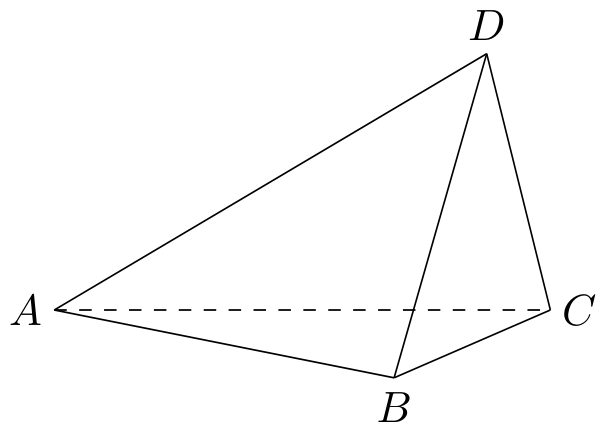
\includegraphics[width=7.5cm]{GaoKao/images/2011/chongqing_liberal/q20_fig1.png}
\end{center}

        \item 如图，椭圆的中心为原点 \(O\)，离心率 \( e = \frac{\sqrt{2}}{2} \)，一条准线的方程是 \( x = 2\sqrt{2} \).
\begin{enumerate}
\item 求该椭圆的标准方程；
\item 设动点 \(P\) 满足： \(\overrightarrow{OP} = \overrightarrow{OM} + 2\overrightarrow{ON}\)，其中 \(M\)，\(N\) 是椭圆上的点，直线 \(OM\) 与 \(ON\) 的斜率之积为 \(-\frac{1}{2}\)，问：是否存在定点 \(F\)，使得 \(|PF|\) 与点 \(P\) 到直线 \(l: x = 2\sqrt{10}\) 的距离之比为定值？ 若存在，求 \(F\) 的坐标；若不存在，说明理由.
\end{enumerate}
\begin{center}
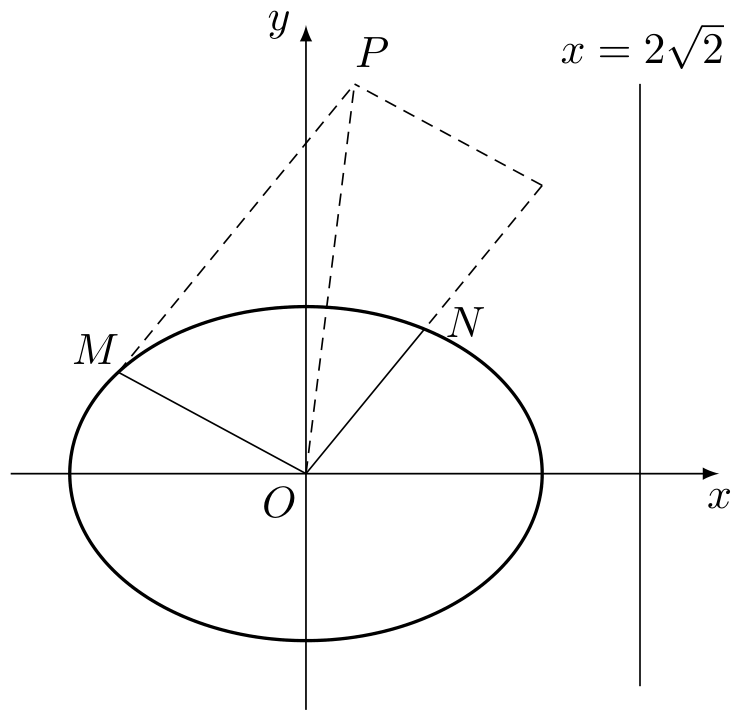
\includegraphics[width=9.3cm]{GaoKao/images/2011/chongqing_liberal/q21_fig1.png}
\end{center}

    \end{enumerate}

\end{description}


\subsection{2011年福建卷（理）}\label{gk:2011年福建卷（理）}

\begin{description}

    \item[一、选择题]

    \begin{enumerate}[leftmargin=5pt]

        \item \(\i\) 是虚数单位，若集合 \(S = \{-1, 0, 1\}\)，则（\quad）

        {\centering\begin{tabular*}{\linewidth}{@{}@{\extracolsep{\fill}}llll@{}}
          \text{A. }\(\i \in S\)  &  \text{B. }\(\i^2\in S\)  &  \text{C. }\(\i^3\in S\)  &  \text{D. }\(\frac{2}{\i} \in S\)
        \end{tabular*}\par}

        \item 若 \(a \in \mathbb{R}\)，则 “\(a = 2\)” 是 “\((a - 1)(a - 2) = 0\)” 的（\quad）

        {\centering\begin{tabular*}{\linewidth}{@{}@{\extracolsep{\fill}}llll@{}}
          \text{A. }充分而不必要条件  &  \text{B. }必要而不充分条件  &  \text{C. }充要条件  &  \text{D. }既不充分也不必要条件
        \end{tabular*}\par}

        \item 若 \(\tan \alpha = 3\)，则 \(\frac{\sin 2\alpha}{\cos^2 \alpha}\) 的值等于（\quad）

        {\centering\begin{tabular*}{\linewidth}{@{}@{\extracolsep{\fill}}llll@{}}
          \text{A. }2  &  \text{B. }3  &  \text{C. }4  &  \text{D. }6
        \end{tabular*}\par}

        \item 如图，矩形 \(ABCD\) 中，点 \(E\) 为边 \(CD\) 的中点，若在矩形 \(ABCD\) 内部随机取一个点 \(Q\)，则点 \(Q\) 取自 \(\triangle ABE\) 内部的概率等于（\quad）

\begin{center}
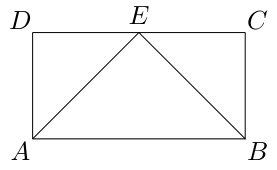
\includegraphics[width=5.7cm]{GaoKao/images/2011/fujian_science/q4_fig1.png}
\end{center}

        {\centering\begin{tabular*}{\linewidth}{@{}@{\extracolsep{\fill}}llll@{}}
          \text{A. }\( \frac{1}{4} \)  &  \text{B. }\( \frac{1}{3} \)  &  \text{C. }\( \frac{1}{2} \)  &  \text{D. }\( \frac{2}{3} \)
        \end{tabular*}\par}

        \item \(\int_{0}^{1}\left({\mathrm{e}}^{x} + 2x\right)\mathrm{d}x\) 等于（\quad）

        {\centering\begin{tabular*}{\linewidth}{@{}@{\extracolsep{\fill}}llll@{}}
          \text{A. }1  &  \text{B. }\({\mathrm{e}}\) - 1  &  \text{C. }\({\mathrm{e}}\)  &  \text{D. }\({\mathrm{e}}\) + 1
        \end{tabular*}\par}

        \item \((1 + 2x)^{5}\) 的展开式中，\(x^{2}\) 的系数等于（\quad）

        {\centering\begin{tabular*}{\linewidth}{@{}@{\extracolsep{\fill}}llll@{}}
          \text{A. }80  &  \text{B. }40  &  \text{C. }20  &  \text{D. }10
        \end{tabular*}\par}

        \item 设圆锥曲线 \(T\) 的两个焦点分别为 \(F_{1}\)，\(F_{2}\). 若曲线 \(T\) 上存在点 \(P\) 满足 \(|PF_{1}|: |F_{1}F_{2}|: |PF_{2}| = 4:3:2\)，则曲线 \(T\) 的离心率等于（\quad）

        {\centering\begin{tabular*}{\linewidth}{@{}@{\extracolsep{\fill}}llll@{}}
          \text{A. }\(\frac{1}{2}\) 或 \(\frac{3}{2}\)  &  \text{B. }\(\frac{2}{3}\) 或 2  &  \text{C. }\(\frac{1}{2}\) 或 2  &  \text{D. }\(\frac{2}{3}\) 或 \(\frac{3}{2}\)
        \end{tabular*}\par}

        \item 已知 \(O\) 是坐标原点，点 \(A(-1,1)\)，若点 \(M(x,y)\) 为平面区域 \(\begin{cases}
x+y\geqslant 2,\\
x\leqslant 1,\\
y\leqslant 2
\end{cases}\) 上的一个动点，则 \(\overrightarrow{OA}\cdot\overrightarrow{OM}\) 的取值范围是（\quad）

        {\centering\begin{tabular*}{\linewidth}{@{}@{\extracolsep{\fill}}llll@{}}
          \text{A. }\([-1,0]\)  &  \text{B. }\([0,1]\)  &  \text{C. }\([0,2]\)  &  \text{D. }\([-1,2]\)
        \end{tabular*}\par}

        \item 对于函数 \(f(x)=a\sin x+bx+c\)（其中 \(a\)，\(b\in\mathbb{R}\)，\(c\in\mathbb{Z}\)），选取 \(a\)，\(b\)，\(c\) 的一组值计算 \(f(1)\) 和 \(f(-1)\)，所得出的正确结果一定不可能是（\quad）

        {\centering\begin{tabular*}{\linewidth}{@{}@{\extracolsep{\fill}}llll@{}}
          \text{A. }4 和 6  &  \text{B. }3 和 1  &  \text{C. }2 和 4  &  \text{D. }1 和 2
        \end{tabular*}\par}

        \item 已知函数 \(f(x)={\mathrm{e}}^{x}+x\). 对于曲线 \(y=f(x)\) 上横坐标成等差数列的三个点 \(A\)，\(B\)，\(C\)，给出以下判断：

\begin{enumerate}
\item \(\triangle ABC\) 一定是钝角三角形；
\item \(\triangle ABC\) 可能是直角三角形；
\item \(\triangle ABC\) 可能是等腰三角形；
\item \(\triangle ABC\) 不可能是等腰三角形.
\end{enumerate}

其中，正确的判断是（\quad）

        {\centering\begin{tabular*}{\linewidth}{@{}@{\extracolsep{\fill}}llll@{}}
          \text{A. }\ding{172}\ding{174}  &  \text{B. }\ding{172}\ding{175}  &  \text{C. }\ding{173}\ding{174}  &  \text{D. }\ding{173}\ding{175}
        \end{tabular*}\par}

    \end{enumerate}

\end{description}

\begin{description}

    \item[二、填空题]

    \begin{enumerate}[leftmargin=5pt]

      \addtocounter{enumi}{+10}

        \item 运行如图所示的程序，输出的结果是\rule[-0.3ex]{3em}{0.4pt}.

\begin{center}
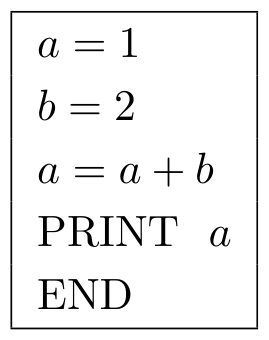
\includegraphics[width=3.3cm]{GaoKao/images/2011/fujian_science/q11_fig1.png}
\end{center}

        \item 三棱锥 \(P - ABC\) 中，\(PA \perp\) 底面 \(ABC\)，\(PA = 3\)，底面 \(ABC\) 是边长为 \(2\) 的正三角形，则三棱锥 \(P - ABC\) 的体积等于\rule[-0.3ex]{3em}{0.4pt}.

        \item 盒中装有形状，大小完全相同的 \(5\) 个球，其中红色球 \(3\) 个，黄色球 \(2\) 个. 若从中随机取出 \(2\) 个球，则所取出的 \(2\) 个球颜色不同的概率等于\rule[-0.3ex]{3em}{0.4pt}.

        \item 如图，\(\triangle ABC\) 中，\(AB = AC = 2\)，\(BC = 2\sqrt{3}\)，点 \(D\) 在 \(BC\) 边上，\(\angle ADC = 45^\circ\)，则 \(AD\) 的长度等于\rule[-0.3ex]{3em}{0.4pt}.

\begin{center}
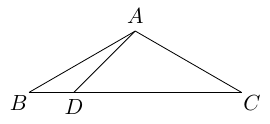
\includegraphics[width=6.5cm]{GaoKao/images/2011/fujian_science/q14_fig1.png}
\end{center}

        \item 设 \(V\) 是全体平面向量构成的集合. 若映射 \(f:V\to\mathbb{R}\) 满足：对任意向量 \(a=(x_1,y_1)\in V\)，\(b=(x_2,y_2)\in V\)，以及任意 \(\lambda\in\mathbb{R}\)，均有 \(f\left(\lambda a+(1-\lambda)b\right)=\lambda f(a)+(1-\lambda)f(b)\)，则称映射 \(f\) 具有性质 \(P\). 现给出如下映射：

\begin{enumerate}
\item \(f_1:V\to\mathbb{R}\)，\(f_1(m)=x-y\)，\(m=(x,y)\in V\)；
\item \(f_2:V\to\mathbb{R}\)，\(f_2(m)=x^2+y\)，\(m=(x,y)\in V\)；
\item \(f_3:V\to\mathbb{R}\)，\(f_3(m)=x+y+1\)，\(m=(x,y)\in V\).
\end{enumerate}

其中，具有性质 \(P\) 的映射的序号为\rule[-0.3ex]{3em}{0.4pt}（写出所有具有性质 \(P\) 的映射的序号）.

    \end{enumerate}

\end{description}

\begin{description}

    \item[三、解答题]

    \begin{enumerate}[leftmargin=5pt]

      \addtocounter{enumi}{+15}

        \item 已知等比数列 \(\{a_n\}\) 的公比 \(q=3\)，前 \(3\) 项和 \(S_3=\frac{13}{3}\).

\begin{enumerate}
\item 求数列 \(\{a_n\}\) 的通项公式；
\item 若函数 \(f(x)=A\sin\left(2x+\varphi\right)\)（\(A>0\)，\(0<\varphi<\pi\)）在 \(x=\frac{\pi}{6}\) 处取得最大值，且最大值为 \(a_3\)，求函数 \(f(x)\) 的解析式.
\end{enumerate}

        \item 已知直线 \(l:y=x+m\)，\(m\in\mathbb{R}\).

\begin{enumerate}
\item 若以点 \(M(2,0)\) 为圆心的圆与直线 \(l\) 相切于点 \(P\)，且点 \(P\) 在 \(y\) 轴上，求该圆的方程；
\item 若直线 \(l\) 关于 \(x\) 轴对称的直线为 \(l'\)，问直线 \(l'\) 与抛物线 \(C:x^2=4y\) 是否相切？说明理由.
\end{enumerate}

        \item 某商场销售某种商品的经验表明，该商品每日的销售量 \(y\)（单位：千克）与销售价格 \(x\)（单位：元/千克）满足关系式 \(y=\frac{a}{x-3}+10(x-6)^2\)，其中 \(3<x<6\)，\(a\) 为常数. 已知销售价格为 \(5\text{ 元/千克}\) 时，每日可售出该商品 \(11\text{ 千克}\).

\begin{enumerate}
\item 求 \(a\) 的值；
\item 若该商品的成本为 \(3\text{ 元/千克}\)，试确定销售价格 \(x\) 的值，使商场每日销售该商品所获得的利润最大.
\end{enumerate}

        \item 某产品按行业生产标准分成 \(8\) 个等级，等级系数 \(X\) 依次为 \(1\)，\(2\)，\(\dots\)，\(8\)，其中 \(X\geqslant 5\) 为标准 \(A\)，\(X\geqslant 3\) 为标准 \(B\). 已知甲厂执行标准 \(A\) 生产该产品，产品的零售价为 \(6\text{ 元/件}\)；乙厂执行标准 \(B\) 生产该产品，产品的零售价为 \(4\text{ 元/件}\)，假定甲，乙两厂的产品都符合相应的执行标准.

\begin{enumerate}
\item 已知甲厂产品的等级系数 \(X_1\) 的概率分布如下表所示：

\begin{center}
\begin{tabular}{|c|c|c|c|c|}
\hline
\(X_1\) & 5 & 6 & 7 & 8 \\
\hline
\(P\) & 0.4 & \(a\) & \(b\) & 0.1 \\
\hline
\end{tabular}
\end{center}

且 \(E(X_1)=6\). 求 \(a\)，\(b\) 的值；
\item 为分析乙厂产品的等级系数 \(X_2\)，从该厂生产的产品中随机抽取 \(30\) 件，相应的等级系数组成一个样本. 数据如下：

\begin{center}
\begin{tabular}{cccccccccc}
3 & 5 & 3 & 3 & 8 & 5 & 5 & 6 & 3 & 4 \\
6 & 3 & 4 & 7 & 5 & 3 & 4 & 8 & 5 & 3 \\
8 & 3 & 4 & 3 & 4 & 4 & 7 & 5 & 6 & 7
\end{tabular}
\end{center}

用这个样本的频率分布估计总体分布，将频率视为概率，求等级系数 \(X_2\) 的数学期望；
\item 在前两问的条件下，若以“性价比”为判断标准，则哪个工厂的产品更具可购买性？说明理由.
\end{enumerate}

注：

\begin{enumerate}
\item 产品的“性价比”\(=\frac{\text{产品的等级系数的数学期望}}{\text{产品的零售价}}\)；
\item “性价比”大的产品更具可购买性.
\end{enumerate}

        \item 如图，四棱锥 \(P-ABCD\) 中，\(PA\perp\) 底面 \(ABCD\)，四边形 \(ABCD\) 中，\(AB\perp AD\)，\(AB+AD=4\)，\(CD=\sqrt{2}\)，\(\angle CDA=45^\circ\).

\begin{enumerate}
\item 求证：平面 \(PAB\perp\) 平面 \(PAD\)；
\item 设 \(AB=AP\).

\begin{enumerate}
\item 若直线 \(PB\) 与平面 \(PCD\) 所成的角为 \(30^\circ\)，求线段 \(AB\) 的长；
\item 在线段 \(AD\) 上是否存在一个点 \(G\)，使得点 \(G\) 到点 \(P\)，\(B\)，\(C\)，\(D\) 的距离都相等？说明理由.
\end{enumerate}
\end{enumerate}

\begin{center}
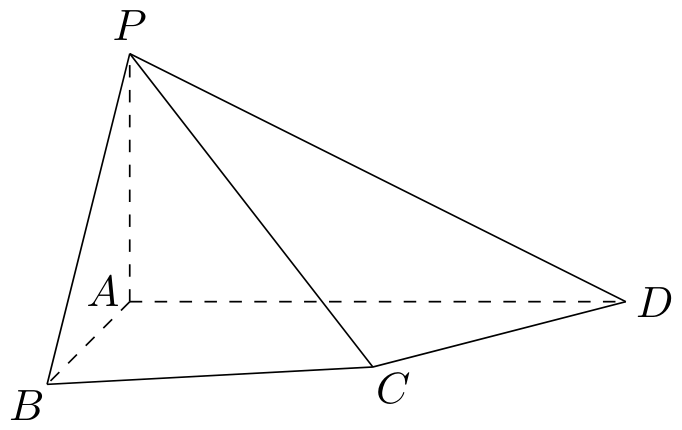
\includegraphics[width=8.5cm]{GaoKao/images/2011/fujian_science/q20_fig1.png}
\end{center}

    \end{enumerate}

\end{description}

\begin{description}

    \item[四、选考题]

    \begin{enumerate}[leftmargin=5pt]

      \addtocounter{enumi}{+20}

        \item 设矩阵 \(M = \begin{pmatrix} a & 0 \\ 0 & b \end{pmatrix}\)（其中 \(a > 0\)，\(b > 0\)）

\begin{enumerate}
\item 若 \(a = 2\)，\(b = 3\)，求矩阵 \(M\) 的逆矩阵 \(M^{-1}\)；
\item 若曲线 \(C: x^{2} + y^{2} = 1\) 在矩阵 \(M\) 所对应的线性变换作用下得到曲线
\(C' : \frac{x^{2}}{4} + y^{2} = 1\)，求 \(a\)，\(b\) 的值.
\end{enumerate}

        \item \textbf{【选修4-4：坐标系与参数方程】}

在直角坐标系 \(xOy\) 中，直线 \(l\) 的方程为 \(x-y+4=0\)，曲线 \(C\) 的参数方程为 \(\begin{cases}
x=\sqrt{3}\cos\alpha,\\
y=\sin\alpha
\end{cases}\)（\(\alpha\) 为参数）.

\begin{enumerate}
\item 已知在极坐标（与直角坐标系 \(xOy\) 取相同的长度单位，且以原点 \(O\) 为极点，以 \(x\) 轴正半轴为极轴）中，点 \(P\) 的极坐标为 \(\left(4,\frac{\pi}{2}\right)\)，判断点 \(P\) 与直线 \(l\) 的位置关系；
\item 设点 \(Q\) 是曲线 \(C\) 上的一个动点，求它到直线 \(l\) 的距离的最小值.
\end{enumerate}

        \item \textbf{【选修4-5：不等式选讲】}

设不等式 \(|2x-1|<1\) 的解集为 \(M\).

\begin{enumerate}
\item 求集合 \(M\)；
\item 若 \(a\)，\(b\in M\)，试比较 \(ab+1\) 与 \(a+b\) 的大小.
\end{enumerate}

    \end{enumerate}

\end{description}


\subsection{2011年福建卷（文）}\label{gk:2011年福建卷（文）}

\begin{description}

    \item[一、选择题]

    \begin{enumerate}[leftmargin=5pt]

        \item 若集合 \(M = \{-1, 0, 1\}\)，\(N = \{0, 1, 2\}\)，则 \(M \cap N\) 等于（\quad）

        {\centering\begin{tabular*}{\linewidth}{@{}@{\extracolsep{\fill}}llll@{}}
          \text{A. }\(\{0, 1\}\)  &  \text{B. }\( \{-1,0,1\} \)  &  \text{C. }\(\{0,1,2\}\)  &  \text{D. }\(\{-1,0,1,2\}\)
        \end{tabular*}\par}

        \item \(\i\) 是虚数单位，\( 1 + \i^{3} \) 等于（\quad）

        {\centering\begin{tabular*}{\linewidth}{@{}@{\extracolsep{\fill}}llll@{}}
          \text{A. }\(\i\)  &  \text{B. }\(-\i\)  &  \text{C. }\(1 + \i\)  &  \text{D. }\(1 - \i\)
        \end{tabular*}\par}

        \item 若 \(a \in \mathbb{R}\)，则“\(a = 1\)”是“\(\lvert a \rvert = 1\)”的（\quad）

        {\centering\begin{tabular*}{\linewidth}{@{}@{\extracolsep{\fill}}llll@{}}
          \text{A. }充分而不必要条件  &  \text{B. }必要而不充分条件  &  \text{C. }充要条件  &  \text{D. }既不充分也不必要条件
        \end{tabular*}\par}

        \item 某校选修乒乓球课程的学生中，高一年级有 30 名，高二年级有 40 名. 现用分层抽样的方法在这 70 名学生中抽取一个样本，已知在高一年级的学生中抽取了 6 名，则在高二年级的学生中应抽取的人数为（\quad）

        {\centering\begin{tabular*}{\linewidth}{@{}@{\extracolsep{\fill}}llll@{}}
          \text{A. }6  &  \text{B. }8  &  \text{C. }10  &  \text{D. }12
        \end{tabular*}\par}

        \item 阅读如图所示的程序框图，运行相应的程序，输出的结果是（\quad）

\begin{center}
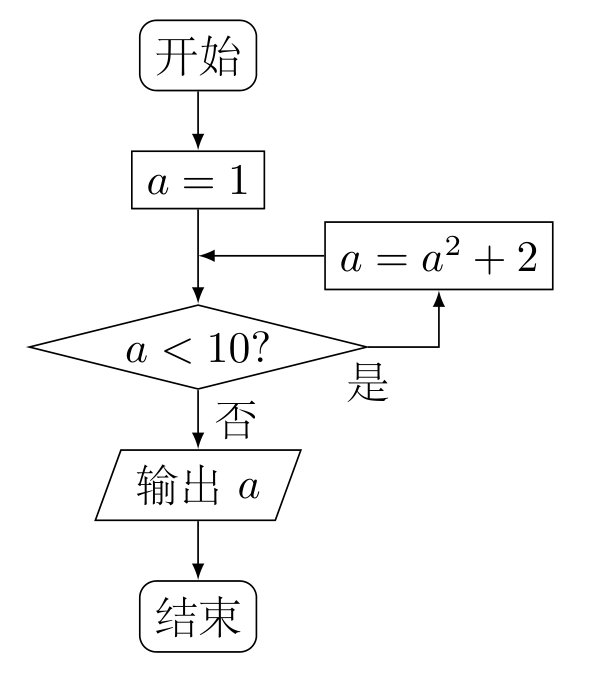
\includegraphics[width=0.34\linewidth]{GaoKao/images/2011/fujian_liberal/q5_fig1.png}
\end{center}

        {\centering\begin{tabular*}{\linewidth}{@{}@{\extracolsep{\fill}}llll@{}}
          \text{A. }3  &  \text{B. }11  &  \text{C. }38  &  \text{D. }123
        \end{tabular*}\par}

        \item 若关于 \(x\) 的方程 \(x^{2} + mx + 1 = 0\) 有两个不相等的实数根，则实数 \(m\) 的取值范围是（\quad）

        {\centering\begin{tabular*}{\linewidth}{@{}@{\extracolsep{\fill}}llll@{}}
          \text{A. }\((-1, 1)\)  &  \text{B. }\((-2, 2)\)  &  \text{C. }\((- \infty, -2) \cup (2, +\infty)\)  &  \text{D. }\((-\infty, -1) \cup (1, +\infty)\)
        \end{tabular*}\par}

        \item 如图，矩形 \(ABCD\) 中，点 \(E\) 为边 \(CD\) 的中点，若在矩形 \(ABCD\) 内部随机取一个点 \(Q\)，则点 \(Q\) 取自 \(\triangle ABE\) 内部的概率等于（\quad）

\begin{center}
\begin{center}
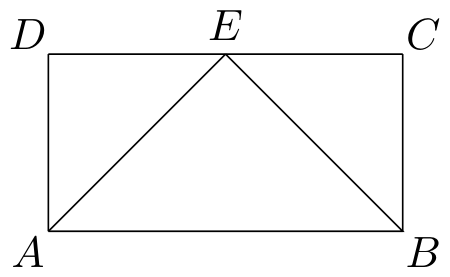
\includegraphics[width=5.6cm]{GaoKao/images/2011/fujian_liberal/q7_fig1.png}
\end{center}
\end{center}

        {\centering\begin{tabular*}{\linewidth}{@{}@{\extracolsep{\fill}}llll@{}}
          \text{A. }\( \frac{1}{4} \)  &  \text{B. }\( \frac{1}{3} \)  &  \text{C. }\( \frac{1}{2} \)  &  \text{D. }\( \frac{2}{3} \)
        \end{tabular*}\par}

        \item 已知函数 \( f(x) = \begin{cases}
2^x, & x > 0,\\
x + 1, & x \leqslant 0.
\end{cases} \) 若 \( f(a) + f(1) = 0 \)，则实数 \( a \) 的值等于（\quad）

        {\centering\begin{tabular*}{\linewidth}{@{}@{\extracolsep{\fill}}llll@{}}
          \text{A. }\(-3\)  &  \text{B. }\(-1\)  &  \text{C. }1  &  \text{D. }3
        \end{tabular*}\par}

        \item 若 \(\alpha \in \left(0, \frac{\pi}{2}\right)\)，且 \(\sin^2\alpha + \cos 2\alpha = \frac{1}{4}\)，则 \(\tan \alpha\) 的值等于（\quad）

        {\centering\begin{tabular*}{\linewidth}{@{}@{\extracolsep{\fill}}llll@{}}
          \text{A. }\(\frac{\sqrt{2}}{2}\)  &  \text{B. }\( \frac{\sqrt{3}}{3} \)  &  \text{C. }\(\sqrt{2}\)  &  \text{D. }\(\sqrt{3}\)
        \end{tabular*}\par}

        \item 若 \(a > 0\)，\(b > 0\)，且函数 \(f(x) = 4x^3 - ax^2 - 2bx + 2\) 在 \(x = 1\) 处有极值，则 \(ab\) 的最大值等于（\quad）

        {\centering\begin{tabular*}{\linewidth}{@{}@{\extracolsep{\fill}}llll@{}}
          \text{A. }2  &  \text{B. }3  &  \text{C. }6  &  \text{D. }9
        \end{tabular*}\par}

        \item 设圆锥曲线 \(\Gamma\) 的两个焦点分别为 \(F_{1}\)，\(F_{2}\). 若曲线 \(\Gamma\) 上存在点 \(P\) 满足 \(|PF_{1}|: |F_{1}F_{2}|: |PF_{2}| = 4:3:2\)，则曲线 \(\Gamma\) 的离心率等于（\quad）

        {\centering\begin{tabular*}{\linewidth}{@{}@{\extracolsep{\fill}}llll@{}}
          \text{A. }\(\frac{1}{2}\) 或 \(\frac{3}{2}\)  &  \text{B. }\(\frac{2}{3}\) 或 2  &  \text{C. }\(\frac{1}{2}\) 或 2  &  \text{D. }\(\frac{2}{3}\) 或 \(\frac{3}{2}\)
        \end{tabular*}\par}

        \item 在整数集 \(\mathbb{Z}\) 中，被 5 除所得余数为 \(k\) 的所有整数组成一个“类”，记为 \([k]\)，即 \([k] = \{5n + k \mid n \in \mathbb{Z}\}\)，\(k = 0\)，\(1\)，\(2\)，\(3\)，\(4\). 给出如下四个结论：

\begin{enumerate}
\item \(2011 \in [1]\)；
\item \(-3 \in [3]\)；
\item \(\mathbb{Z} = [0] \cup [1] \cup [2] \cup [3] \cup [4]\)；
\item “整数 \(a\)，\(b\) 属于同一‘类’”的充要条件是 “\(a - b \in [0]\)”.
\end{enumerate}

其中，正确结论的个数是（\quad）

        {\centering\begin{tabular*}{\linewidth}{@{}@{\extracolsep{\fill}}llll@{}}
          \text{A. }1  &  \text{B. }2  &  \text{C. }3  &  \text{D. }4
        \end{tabular*}\par}

    \end{enumerate}

\end{description}

\begin{description}

    \item[二、填空题]

    \begin{enumerate}[leftmargin=5pt]

      \addtocounter{enumi}{+12}

        \item 若向量 \(\bm{a}=(1,1)\)，\(\bm{b}=(-1,2)\)，则 \(\bm{a} \cdot \bm{b}\) 等于\rule[-0.3ex]{3em}{0.4pt}.

        \item 若 \(\triangle ABC\) 的面积为 \(\sqrt{3}\)，\(BC = 2\)，\(C = 60^{\circ}\)，则边 \(AB\) 的长度等于\rule[-0.3ex]{3em}{0.4pt}.

        \item 如图，正方体 \(ABCD - A_{1}B_{1}C_{1}D_{1}\) 中，\(AB = 2\)，点 \(E\) 为 \(AD\) 的中点，点 \(F\) 在 \(CD\) 上，

若 \(EF \parallel\) 平面 \(AB_{1}C\)，则线段 \(EF\) 的长度等于\rule[-0.3ex]{3em}{0.4pt}.

\begin{center}
\begin{center}
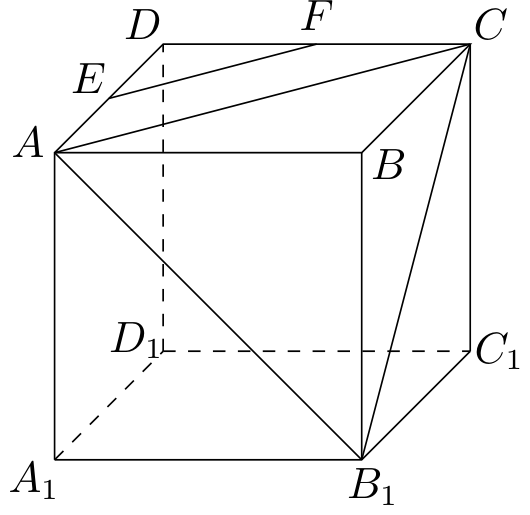
\includegraphics[width=5.3cm]{GaoKao/images/2011/fujian_liberal/q15_fig1.png}
\end{center}
\end{center}

        \item 商家通常依据“乐观系数准则”确定商品销售价格，即根据商品的最低销售限价 \(a\)，最高销售限价 \(b\)（\(b > a\)）以及实数 \(x\)（\(0 < x < 1\)）确定实际销售价格 \( c = a + x (b - a) \). 这里，\(x\) 被称为乐观系数. 经验表明，最佳乐观系数 \(x\) 恰好使得 \( (c - a) \) 是 \( (b - c) \) 和 \( (b - a) \) 的等比中项. 据此可得，最佳乐观系数 \(x\) 的值等于\rule[-0.3ex]{3em}{0.4pt}.

    \end{enumerate}

\end{description}

\begin{description}

    \item[三、解答题]

    \begin{enumerate}[leftmargin=5pt]

      \addtocounter{enumi}{+16}

        \item 已知等差数列 \(\{a_{n}\}\) 中，\(a_{1} = 1\)，\(a_{3} = -3\).

\begin{enumerate}
\item 求数列 \( \{a_{n}\} \) 的通项公式；
\item 若数列 \( \{a_{n}\} \) 的前 \(k\) 项和 \( S_{k} = -35 \)，求 \(k\) 的值.
\end{enumerate}

        \item 如图，直线 \(l\)：\(y = x + b\) 与抛物线 \(C\)：\(x^2 = 4y\) 相切于点 \(A\).

\begin{enumerate}
\item 求实数 \(b\) 的值；
\item 求以点 \(A\) 为圆心，且与抛物线 \(C\) 的准线相切的圆的方程.
\end{enumerate}

\begin{center}
\begin{center}
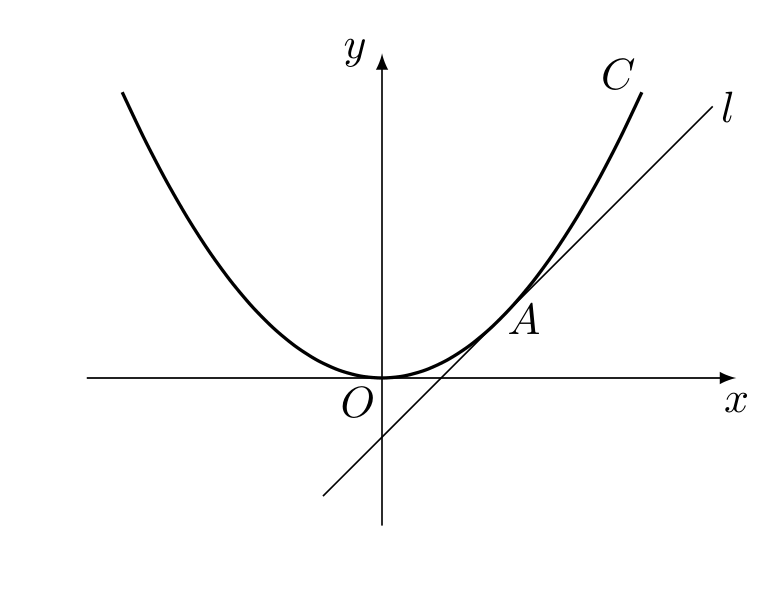
\includegraphics[width=9.0cm]{GaoKao/images/2011/fujian_liberal/q18_fig1.png}
\end{center}
\end{center}

        \item 某日用品按行业质量标准分成五个等级. 等级系数 \(X\) 依次为 \(1\)，\(2\)，\(3\)，\(4\)，\(5\). 现从一批该日用品中随机抽取 20 件，对其等级系数进行统计分析，得到频率分布表如下：

\begin{center}
\begin{tabular}{c|ccccc}
\(X\) & \(1\) & \(2\) & \(3\) & \(4\) & \(5\) \\
\hline
\(f\) & \(a\) & \(0.2\) & \(0.45\) & \(b\) & \(c\)
\end{tabular}
\end{center}

\begin{enumerate}
\item 若所抽取的 20 件日用品中，等级系数为 4 的恰有 3 件，等级系数为 5 的恰有 2 件，求 \(a\)，\(b\)，\(c\) 的值；
\item 在上问的条件下，将等级系数为 4 的 3 件日用品记为 \(x_{1}\)，\(x_{2}\)，\(x_{3}\)，等级系数为 5 的 2 件日用品记为 \(y_{1}\)，\(y_{2}\). 现从 \(x_{1}\)，\(x_{2}\)，\(x_{3}\)，\(y_{1}\)，\(y_{2}\) 这 5 件日用品中任取两件（假定每件日用品被取出的可能性相同），写出所有可能的结果，并求这两件日用品的等级系数恰好相等的概率.
\end{enumerate}

        \item 如图，四棱锥 \(P - ABCD\) 中，\(PA \perp\) 底面 \(ABCD\)，\(AB \perp AD\)，点 \(E\) 在线段 \(AD\) 上，且 \(CE \parallel AB\).

\begin{enumerate}
\item 求证：\( CE \perp \) 平面 \(PAD\)；
\item 若 \(PA = AB = 1\)，\(AD = 3\)，\(CD = \sqrt{2}\)，\(\angle CDA = 45^{\circ}\)，求四棱锥 \(P - ABCD\) 的体积.
\end{enumerate}

\begin{center}
\begin{center}
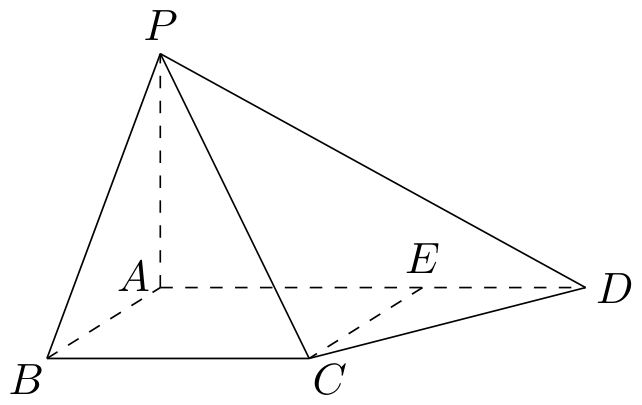
\includegraphics[width=6.3cm]{GaoKao/images/2011/fujian_liberal/q20_fig1.png}
\end{center}
\end{center}

        \item 设函数 \( f(\theta) = \sqrt{3}\sin \theta + \cos \theta \)，其中，角 \( \theta \) 的顶点与坐标原点重合，始边与 \( x \) 轴非负半轴重合，终边经过点 \( P(x, y) \)，且 \( 0 \leqslant \theta \leqslant \pi \).

\begin{enumerate}
\item 若点 \(P\) 的坐标为 \(\left(\frac{1}{2}, \frac{\sqrt{3}}{2}\right)\)，求 \(f(\theta)\) 的值；
\item 若点 \(P(x, y)\) 为平面区域 \(\Omega\)：\(\begin{cases}
x + y \geqslant 1,\\
x \leqslant 1,\\
y \leqslant 1
\end{cases}\) 上的一个动点，试确定角 \(\theta\) 的取值范围，并求函数 \(f(\theta)\) 的最小值和最大值.
\end{enumerate}

        \item 已知 \(a\)，\(b\) 为常数，且 \(a \neq 0\). 函数 \(f(x) = -ax + b + ax \ln x\)，\(f({\mathrm{e}}) = 2\)（\({\mathrm{e}} = 2.71828 \cdots\) 是自然对数的底数）.

\begin{enumerate}
\item 求实数 \(b\) 的值；
\item 求函数 \( f(x) \) 的单调区间；
\item 当 \(a = 1\) 时，是否同时存在实数 \(m\) 和 \(M\)（\(m < M\)），使得对每一个 \(t \in [m, M]\)，直线 \(y = t\) 与曲线 \(y = f(x)\)（\(x \in \left[ \frac{1}{2}, {\mathrm{e}} \right]\)）都有公共点？若存在，求出最小的实数 \(m\) 和最大的实数 \(M\)；若不存在，说明理由.
\end{enumerate}

    \end{enumerate}

\end{description}


\subsection{2011年广东卷（理）}\label{gk:2011年广东卷（理）}

\begin{description}

    \item[一、选择题]

    \begin{enumerate}[leftmargin=5pt]

        \item 设复数 \(z\) 满足 \((1 + \i)z = 2\)，其中 \(\i\) 为虚数单位，则 \(z =\)（\quad）

        {\centering\begin{tabular*}{\linewidth}{@{}@{\extracolsep{\fill}}llll@{}}
          \text{A. }\(1 + \i\)  &  \text{B. }\(1 - \i\)  &  \text{C. }\(2 + 2\i\)  &  \text{D. }\(2 - 2\i\)
        \end{tabular*}\par}

        \item 已知集合 \(A = \{(x, y) | x, y\) 为实数，且 \(x^2 + y^2 = 1\}\)，\(B = \{(x, y) | x, y\) 为实数，且 \(y = x\}\)，则 \(A \cap B\) 的元素个数为（\quad）

        {\centering\begin{tabular*}{\linewidth}{@{}@{\extracolsep{\fill}}llll@{}}
          \text{A. }\(0\)  &  \text{B. }\(1\)  &  \text{C. }\(2\)  &  \text{D. }\(3\)
        \end{tabular*}\par}

        \item 若非零向量 \(a\)，\(b\)，\(c\) 满足 \(a \parallel b\) 且 \(a \perp c\)，则 \(c \cdot (a + 2b) =\)（\quad）

        {\centering\begin{tabular*}{\linewidth}{@{}@{\extracolsep{\fill}}llll@{}}
          \text{A. }\(4\)  &  \text{B. }\(3\)  &  \text{C. }\(2\)  &  \text{D. }\(0\)
        \end{tabular*}\par}

        \item 设函数 \( f(x) \) 和 \( g(x) \) 分别是 \( \mathbb{R} \) 上的偶函数和奇函数，则下列结论恒成立的是（\quad）

        {\centering\begin{tabular*}{\linewidth}{@{}@{\extracolsep{\fill}}llll@{}}
          \text{A. }\(f(x) + |g(x)|\) 是偶函数  &  \text{B. }\(f(x) - |g(x)|\) 是奇函数  &  \text{C. }\(|f(x)| + g(x)\) 是偶函数  &  \text{D. }\( |f(x)| - g(x) \) 是奇函数
        \end{tabular*}\par}

        \item 已知平面直角坐标系 \(xOy\) 上的区域 \(D\) 由不等式组 \(\begin{cases}
0 \leqslant x \leqslant \sqrt{2},\\
y \leqslant 2,\\
x \leqslant \sqrt{2} y
\end{cases}\) 给定. 若 \(M(x,y)\) 为 \(D\) 上的动点，点 \(A\) 的坐标为 \((\sqrt{2},1)\)，则 \(z = \overrightarrow{OM} \cdot \overrightarrow{OA}\) 的最大值为（\quad）

        {\centering\begin{tabular*}{\linewidth}{@{}@{\extracolsep{\fill}}llll@{}}
          \text{A. }\(4\sqrt{2}\)  &  \text{B. }\(3\sqrt{2}\)  &  \text{C. }4  &  \text{D. }3
        \end{tabular*}\par}

        \item 甲，乙两队进行排球决赛. 现在的情形是甲队只要再赢一局就获冠军，乙队需要再赢两局才能得冠军. 若两队胜每局的概率相同，则甲队获得冠军的概率为（\quad）

        {\centering\begin{tabular*}{\linewidth}{@{}@{\extracolsep{\fill}}llll@{}}
          \text{A. }\(\frac{1}{2}\)  &  \text{B. }\( \frac{3}{5} \)  &  \text{C. }\( \frac{2}{3} \)  &  \text{D. }\( \frac{3}{4} \)
        \end{tabular*}\par}

        \item 如图，某几何体的正视图（主视图）是平行四边形，侧视图（左视图）和俯视图都是矩形，则该几何体的体积为（\quad）

\begin{center}
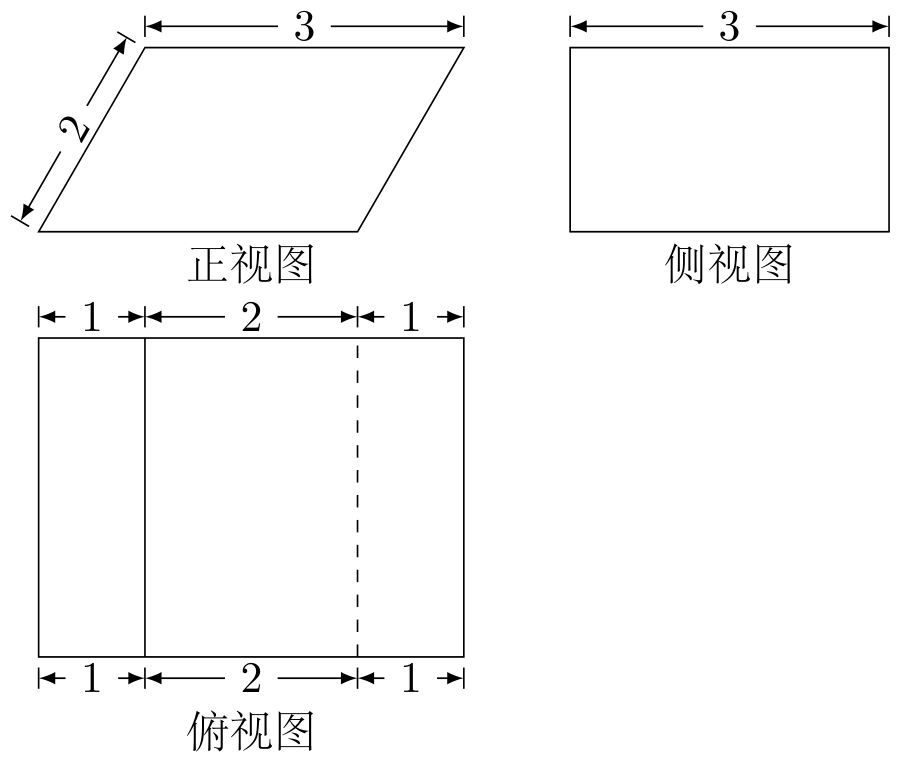
\includegraphics[width=8.8cm]{GaoKao/images/2011/guangdong_science/q7_fig1.png}
\end{center}

        {\centering\begin{tabular*}{\linewidth}{@{}@{\extracolsep{\fill}}llll@{}}
          \text{A. }\(6\sqrt{3}\)  &  \text{B. }\(9\sqrt{3}\)  &  \text{C. }\(12\sqrt{3}\)  &  \text{D. }\(18\sqrt{3}\)
        \end{tabular*}\par}

        \item 设 \(S\) 是整数集 \(\mathbb{Z}\) 的非空子集，如果对于 \(\forall a,b\in S\)，有 \(ab \in S\)，则称 \(S\) 关于数的乘法是封闭的. 若 \(T\)，\(V\) 是 \(\mathbb{Z}\) 的两个不相交的非空子集，\(T \cup V = \mathbb{Z}\). 且对于 \(\forall a,b,c\in T\)，有 \(abc \in T\)，\(\forall x,y,z\in V\)，有 \(xyz \in V\). 则下列结论恒成立的是（\quad）

        {\centering\begin{tabular*}{\linewidth}{@{}@{\extracolsep{\fill}}llll@{}}
          \text{A. }\(T\)，\( V\) 中至少有一个关于乘法是封闭的  &  \text{B. }\(T\)，\(V\) 中至多有一个关于乘法是封闭的  &  \text{C. }\(T\)，\(V\) 中有且只有一个关于乘法是封闭的  &  \text{D. }\(T\)，\(V\) 中每一个关于乘法都是封闭的
        \end{tabular*}\par}

    \end{enumerate}

\end{description}

\begin{description}

    \item[二、填空题]

    \begin{enumerate}[leftmargin=5pt]

      \addtocounter{enumi}{+8}

        \item 不等式 \(|x + 1| - |x - 3| \geqslant 0\) 的解集是\rule[-0.3ex]{3em}{0.4pt}.

        \item \(x\left(x - \frac{2}{x}\right)^7\) 的展开式中，\(x^4\) 的系数是\rule[-0.3ex]{3em}{0.4pt}. （用数字作答）

        \item 等差数列 \(\{a_{n}\}\) 前9项的和等于前4项的和. 若 \(a_{1} = 1\)，\(a_{k} + a_{4} = 0\)，则 \(k = \)\rule[-0.3ex]{3em}{0.4pt}.

        \item 函数 \( f(x) = x^3 - 3x^2 + 1 \) 在 \( x =\rule[-0.3ex]{3em}{0.4pt} \) 处取得极小值.

        \item 某数学老师身高 \(176\mathrm{~cm}\)，他爷爷，父亲和儿子的身高分别是 \(173\mathrm{~cm}\)，\(170\mathrm{~cm}\) 和 \(182\mathrm{~cm}\). 因儿子的身高与父亲的身高有关，该老师用线性回归分析的方法预测他孙子的身高为\rule[-0.3ex]{3em}{0.4pt}\(\mathrm{cm}\).

    \end{enumerate}

\end{description}

\begin{description}

    \item[三、选考题]

    \begin{enumerate}[leftmargin=5pt]

      \addtocounter{enumi}{+13}

        \item \textbf{【选修4-4：坐标系与参数方程】}

已知两曲线参数方程分别为 \(\begin{cases}
x = \sqrt{5} \cos \theta,\\
y = \sin \theta,
\end{cases}\)（\(0 \leqslant \theta < \pi\)）和 \(\begin{cases}
x = \frac{5}{4} t^2,\\
y = t,
\end{cases}\)（\(t \in \mathbb{R}\)），它们的交点坐标为\rule[-0.3ex]{3em}{0.4pt}.

        \item \textbf{【选修4-1：几何证明选讲】}

如图，过圆 \(O\) 外一点 \(P\) 分别作圆的切线和割线，交于 \(A\)，\(B\)，且 \(PB = 7\)，\(C\) 是圆上一点，使得 \(BC = 5\)，\(\angle BAC = \angle APB\)，则 \(AB =\rule[-0.3ex]{3em}{0.4pt}\).

\begin{center}
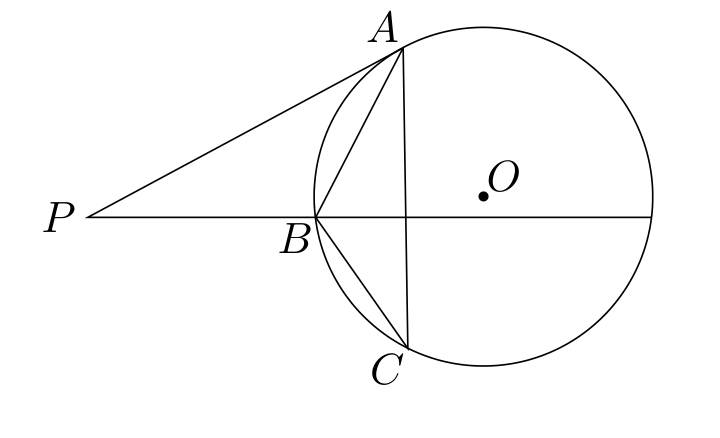
\includegraphics[width=6.5cm]{GaoKao/images/2011/guangdong_science/q15_fig1.png}
\end{center}

    \end{enumerate}

\end{description}

\begin{description}

    \item[四、解答题]

    \begin{enumerate}[leftmargin=5pt]

      \addtocounter{enumi}{+15}

        \item \begin{enumerate}
\item 已知函数 \(f(x) = 2\sin \left(\frac{1}{3} x - \frac{\pi}{6}\right)\)，\(x \in \mathbb{R}\). 求 \( f\left(\frac{5\pi}{4}\right) \) 的值.
\item 设 \(\alpha\)，\(\beta \in \left[0, \frac{\pi}{2}\right]\)，\(f\left(3\alpha + \frac{\pi}{2}\right) = \frac{10}{13}\)，\(f(3\beta + 2\pi) = \frac{6}{5}\)，求 \(\cos (\alpha + \beta)\) 的值.
\end{enumerate}

        \item 为了解甲，乙两厂的产品质量，采用分层抽样的方法从甲，乙两厂生产的产品中分别抽取 14 件和 5 件，测量产品中微量元素 \(x\)，\(y\) 的含量（单位：毫克）. 下表是乙厂的 5 件产品的测量数据：

\begin{center}
\begin{tabular}{|c|c|c|c|c|c|}
\hline
编号 & 1 & 2 & 3 & 4 & 5 \\
\hline
\(x\) & 169 & 178 & 166 & 175 & 180 \\
\hline
\(y\) & 75 & 80 & 77 & 70 & 81 \\
\hline
\end{tabular}
\end{center}

\begin{enumerate}
\item 已知甲厂生产的产品共有 98 件，求乙厂生产的产品数量.
\item 当产品中的微量元素 \(x\)，\(y\) 满足 \(x \geqslant 175\) 且 \(y \geqslant 75\) 时，该产品为优等品. 用上述样本数据估计乙厂生产的优等品的数量.
\item 从乙厂抽出的上述 5 件产品中，随机抽取 2 件，求抽取的 2 件产品中优等品数 \(\xi\) 的分布列及其均值（即数学期望）.
\end{enumerate}

        \item 如图，在锥体 \(P - ABCD\) 中，\(ABCD\) 是边长为 1 的菱形，且 \(\angle DAB = 60^{\circ}\)，\(PA = PD = \sqrt{2}\)，\(PB = 2\)，\(E\)，\(F\) 分别是 \(BC\)，\(PC\) 的中点.

\begin{enumerate}
\item 证明：\(AD \perp\) 平面 \(DEF\).
\item 求二面角 \(P-AD-B\) 的余弦值.
\end{enumerate}

\begin{center}
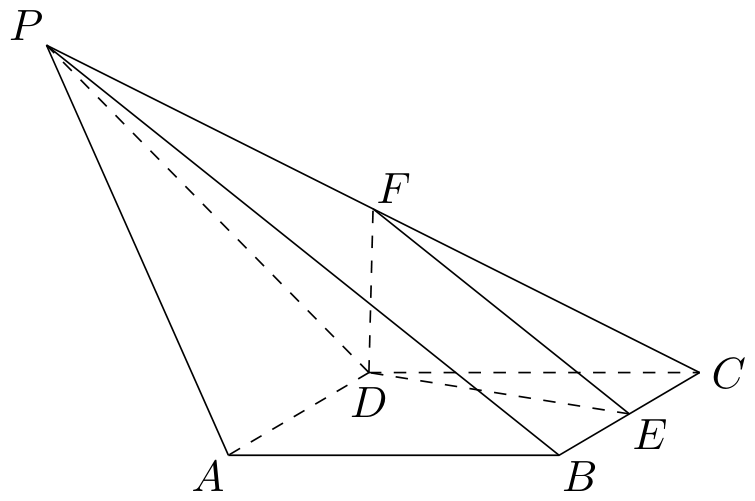
\includegraphics[width=9.4cm]{GaoKao/images/2011/guangdong_science/q18_fig1.png}
\end{center}

        \item \begin{enumerate}
\item 设圆 \(C\) 与两圆 \((x + \sqrt{5})^2 + y^2 = 4\)，\((x - \sqrt{5})^2 + y^2 = 4\) 中的一个内切，另一个外切. 求 \(C\) 的圆心轨迹 \(L\) 的方程.
\item 已知点 \(M\left(\frac{3\sqrt{5}}{5}, \frac{4\sqrt{5}}{5}\right)\)，\(F(\sqrt{5}, 0)\)，且 \(P\) 为 \(L\) 上动点，求 \(\|MP\| - \|FP\|\) 的最大值及此时点 \(P\) 的坐标.
\end{enumerate}

        \item \begin{enumerate}
\item 设 \(b > 0\)，数列 \(\{a_{n}\}\) 满足 \(a_{1} = b\)，\(a_{n} = \frac{nba_{n-1}}{a_{n-1} + 2n - 2}\)（\(n \geqslant 2\)）. 求数列 \(\{a_{n}\}\) 的通项公式.
\item 证明：对于一切正整数 \(n\)，\(a_{n} \leqslant \frac{b^{n+1}}{2^{n+1}} + 1\).
\end{enumerate}

        \item \begin{enumerate}
\item 在平面直角坐标系 \(xOy\) 上，给定抛物线 \(L: y = \frac{1}{4} x^2\). 实数 \(p\)，\(q\) 满足 \(p^2 - 4q \geqslant 0\)，\(x_1\)，\(x_2\) 是方程 \(x^2 - px + q = 0\) 的两根. 记 \(\varphi(p, q) = \max \{|x_1|, |x_2|\}\). 过点 \(A\left(p_0, \frac{1}{4} p_0^2\right)\)（\(p_0 \neq 0\)）作 \(L\) 的切线交 \(y\) 轴于点 \(B\). 证明：对线段 \(AB\) 上的任一点 \(Q(p, q)\)，有 \(\varphi(p, q) = \frac{|p_0|}{2}\).
\item 设 \(M(a, b)\) 是定点，其中 \(a\)，\(b\) 满足 \(a^2 - 4b > 0\)，\(a \neq 0\). 过点 \(M(a, b)\) 作 \(L\) 的两条切线 \(l_1\)，\(l_2\)，切点分别为 \(E\left(p_1, \frac{1}{4} p_1^2\right)\)，\(E'\left(p_2, \frac{1}{4} p_2^2\right)\)，\(l_1\)，\(l_2\) 与 \(y\) 分别交于 \(F\)，\(F'\). 线段 \(EF\) 上异于两端点的点集记为 \(X\). 证明：\(M(a, b) \in X \Leftrightarrow |p_1| > |p_2| \Leftrightarrow \varphi(a, b) = \frac{|p_1|}{2}\).
\item 设 \(D = \left\{(x, y) \mid y \leqslant x - 1, y \geqslant \frac{1}{4} (x + 1)^2 - \frac{5}{4}\right\}\). 当点 \((p, q)\) 取遍 D 时，求 \(\varphi(p, q)\) 的最小值（记为 \(\varphi_{\min}\)）和最大值（记为 \(\varphi_{\max}\)）.
\end{enumerate}

    \end{enumerate}

\end{description}


\subsection{2011年广东卷（文）}\label{gk:2011年广东卷（文）}

\begin{description}

    \item[一、选择题]

    \begin{enumerate}[leftmargin=5pt]

        \item 设复数 \(z\) 满足 \(\i z = 1\)，其中 \(\i\) 为虚数单位，则 \(z =\)（\quad）

        {\centering\begin{tabular*}{\linewidth}{@{}@{\extracolsep{\fill}}llll@{}}
          \text{A. }\(-\i\)  &  \text{B. }\(\i\)  &  \text{C. }\(-1\)  &  \text{D. }\(1\)
        \end{tabular*}\par}

        \item 已知集合 \(A = \{(x, y) | x, y\) 为实数，且 \(x^2 + y^2 = 1\}\)，\(B = \{(x, y) | x, y\) 为实数，且 \(x + y = 1\}\)，则 \(A \cap B\) 的元素个数为（\quad）

        {\centering\begin{tabular*}{\linewidth}{@{}@{\extracolsep{\fill}}llll@{}}
          \text{A. }\(4\)  &  \text{B. }\(3\)  &  \text{C. }\(2\)  &  \text{D. }\(1\)
        \end{tabular*}\par}

        \item 已知向量 \(\bm{a} = (1, 2)\)，\(\bm{b} = (1, 0)\)，\(\bm{c} = (3, 4)\). 若 \(\lambda\) 为实数，\((\bm{a} + \lambda \bm{b}) \parallel \bm{c}\)，则 \(\lambda = \)（\quad）

        {\centering\begin{tabular*}{\linewidth}{@{}@{\extracolsep{\fill}}llll@{}}
          \text{A. }\( \frac{1}{4} \)  &  \text{B. }\( \frac{1}{2} \)  &  \text{C. }\(1\)  &  \text{D. }\(2\)
        \end{tabular*}\par}

        \item 函数 \( f(x) = \frac{1}{1 - x} + \lg (1 + x) \) 的定义域是（\quad）

        {\centering\begin{tabular*}{\linewidth}{@{}@{\extracolsep{\fill}}llll@{}}
          \text{A. }\((-\infty, -1)\)  &  \text{B. }\((1, +\infty)\)  &  \text{C. }\((-1,1)\cup (1, + \infty)\)  &  \text{D. }\((-\infty, +\infty)\)
        \end{tabular*}\par}

        \item 不等式 \(2x^{2} - x - 1 > 0\) 的解集是（\quad）

        {\centering\begin{tabular*}{\linewidth}{@{}@{\extracolsep{\fill}}llll@{}}
          \text{A. }\( \left(-\frac{1}{2},1\right) \)  &  \text{B. }\((1, + \infty)\)  &  \text{C. }\((-\infty, 1) \cup (2, +\infty)\)  &  \text{D. }\(\left(-\infty, -\frac{1}{2}\right) \cup (1, +\infty)\)
        \end{tabular*}\par}

        \item 已知平面直角坐标系 \(xOy\) 上的区域 \(D\) 由不等式组 \(\begin{cases}
0 \leqslant x \leqslant \sqrt{2},\\
y \leqslant 2,\\
x \leqslant \sqrt{2}y
\end{cases}\) 给定。若 \(M(x, y)\) 为 \(D\) 上的动点，点 \(A\) 的坐标为 \((\sqrt{2}, 1)\)，则 \(z = \overrightarrow{OM} \cdot \overrightarrow{OA}\) 的最大值为（\quad）

        {\centering\begin{tabular*}{\linewidth}{@{}@{\extracolsep{\fill}}llll@{}}
          \text{A. }\(3\)  &  \text{B. }\(4\)  &  \text{C. }\( 3\sqrt{2} \)  &  \text{D. }\(4\sqrt{2}\)
        \end{tabular*}\par}

        \item 正五棱柱中，不同在任何侧面且不同在任何底面的两顶点的连线称为它的对角线，那么一个正五棱柱对角线的条数共有（\quad）

        {\centering\begin{tabular*}{\linewidth}{@{}@{\extracolsep{\fill}}llll@{}}
          \text{A. }\(20\)  &  \text{B. }\(15\)  &  \text{C. }\(12\)  &  \text{D. }\(10\)
        \end{tabular*}\par}

        \item 设圆 \(C\) 与圆 \(x^{2}+(y-3)^{2}=1\) 外切，且与直线 \(y=0\) 相切，则 \(C\) 的圆心轨迹为（\quad）

        {\centering\begin{tabular*}{\linewidth}{@{}@{\extracolsep{\fill}}llll@{}}
          \text{A. }抛物线  &  \text{B. }双曲线  &  \text{C. }椭圆  &  \text{D. }圆
        \end{tabular*}\par}

        \item 如图，某几何体的正视图（主视图）、侧视图（左视图）和俯视图分别是等边三角形、等腰三角形和菱形，则该几何体的体积为（\quad）

\begin{center}
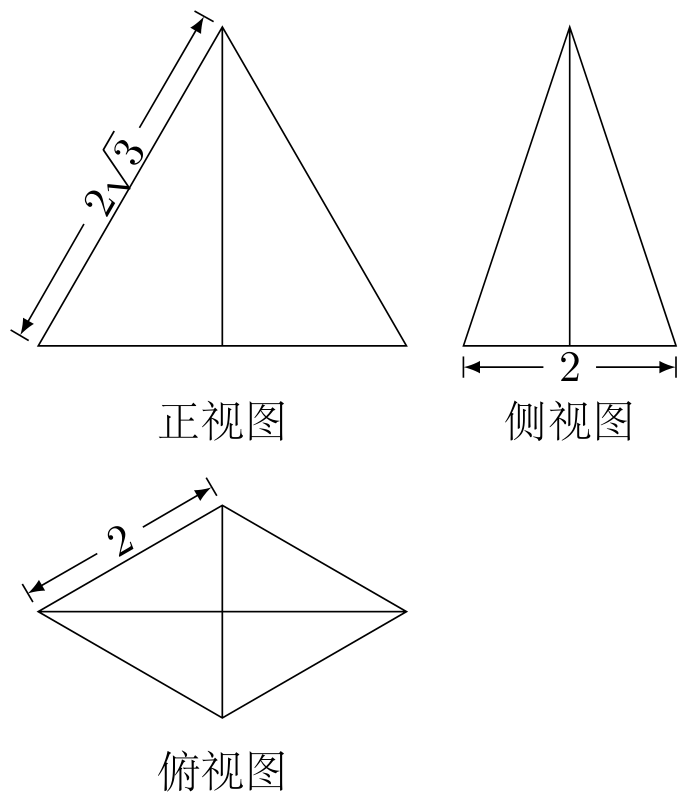
\includegraphics[width=6.8cm]{GaoKao/images/2011/guangdong_liberal/q9_fig1.png}
\end{center}

        {\centering\begin{tabular*}{\linewidth}{@{}@{\extracolsep{\fill}}llll@{}}
          \text{A. }\(4\sqrt{3}\)  &  \text{B. }\(4\)  &  \text{C. }\(2 \sqrt{3}\)  &  \text{D. }\(2\)
        \end{tabular*}\par}

        \item 设 \(f(x)\)，\(g(x)\)，\(h(x)\) 是 \(\mathbb{R}\) 上的任意实值函数. 如下定义两个函数 \((f \circ g)(x)\) 和 \((f \bullet g)(x)\)：对任意 \(x \in \mathbb{R}\)，\((f \circ g)(x) = f(g(x))\)；\((f \bullet g)(x) = f(x)g(x)\)，则下列等式恒成立的是（\quad）

        {\centering\begin{tabular*}{\linewidth}{@{}@{\extracolsep{\fill}}llll@{}}
          \text{A. }\(\big((f\circ g)\bullet h\big)(x) = \big((f\bullet h)\circ (g\bullet h)\big)(x)\)  &  \text{B. }\(\big((f\bullet g)\circ h\big)(x) = \big((f\circ h)\bullet (g\circ h)\big)(x)\)  &  \text{C. }\(\big((f\circ g)\circ h\big)(x) = \big((f\circ h)\circ (g\circ h)\big)(x)\)  &  \text{D. }\(\big((f\bullet g)\bullet h\big)(x) = \big((f\bullet h)\bullet (g\bullet h)\big)(x)\)
        \end{tabular*}\par}

    \end{enumerate}

\end{description}

\begin{description}

    \item[二、填空题]

    \begin{enumerate}[leftmargin=5pt]

      \addtocounter{enumi}{+10}

        \item 已知 \(\{a_{n}\}\) 是递增的等比数列，\(a_{2} = 2\)，\(a_{4} - a_{3} = 4\). 则此数列的公比 \(q = \)\rule[-0.3ex]{3em}{0.4pt}.

        \item 设函数 \( f(x) = x^{3}\cos x + 1 \). 若 \( f(a) = 11 \)，则 \( f(-a) = \)\rule[-0.3ex]{3em}{0.4pt}.

        \item 为了解篮球爱好者小李的投篮命中率与打篮球时间之间的关系. 下表记录了小李某月 \(1\) 号到 \(5\) 号每天打篮球时间 \(x\)（单位：小时）与当天投篮命中率 \(y\) 之间的关系：

\begin{center}
\begin{tabular}{c|ccccc}
时间 \(x\) & \(1\) & \(2\) & \(3\) & \(4\) & \(5\) \\
\hline
命中率 \(y\) & \(0.4\) & \(0.5\) & \(0.6\) & \(0.6\) & \(0.4\)
\end{tabular}
\end{center}

小李这 5 天的平均投篮命中率为\rule[-0.3ex]{3em}{0.4pt}；用线性回归分析的方法，预测小李该月 6 号打 6 小时篮球的投篮命中率为\rule[-0.3ex]{3em}{0.4pt}.

    \end{enumerate}

\end{description}

\begin{description}

    \item[三、选考题]

    \begin{enumerate}[leftmargin=5pt]

      \addtocounter{enumi}{+13}

        \item \textbf{【选修4-4：坐标系与参数方程】}

已知两曲线参数方程分别为 \(\begin{cases}
x = \sqrt{5} \cos \theta,\\
y = \sin \theta,
\end{cases}\) （\(0 \leqslant \theta < \pi\)） 和 \(\begin{cases}
x = \frac{5}{4} t^2,\\
y = t,
\end{cases}\) （\(t \in \mathbb{R}\)） ，它们的交点坐标为\rule[-0.3ex]{3em}{0.4pt}.

        \item 如图，在梯形 \(ABCD\) 中，\(AB \parallel CD\)，\(AB = 4\)，\(CD = 2\)，\(E\)，\(F\) 分别为 \(AD\)，\(BC\) 上的点，且 \(EF = 3\)，\(EF \parallel AB\)，则梯形 \(ABFE\) 与梯形 \(EFCD\) 的面积比为\rule[-0.3ex]{3em}{0.4pt}.

\begin{center}
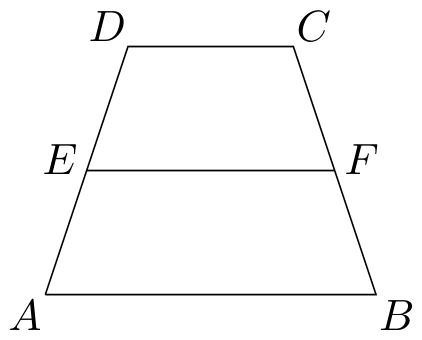
\includegraphics[width=5.1cm]{GaoKao/images/2011/guangdong_liberal/q15_fig1.png}
\end{center}

    \end{enumerate}

\end{description}

\begin{description}

    \item[四、解答题]

    \begin{enumerate}[leftmargin=5pt]

      \addtocounter{enumi}{+15}

        \item 已知函数 \(f(x) = 2\sin \left(\frac{1}{3} x - \frac{\pi}{6}\right)\)，\(x \in \mathbb{R}\).
\begin{enumerate}
\item 求 \( f(0) \) 的值；
\item 设 \(\alpha\)，\(\beta \in \left[0, \frac{\pi}{2}\right]\)，\(f\left(3\alpha + \frac{\pi}{2}\right) = \frac{10}{13}\)，\(f(3\beta + 2\pi) = \frac{6}{5}\)，求 \(\sin (\alpha + \beta)\) 的值.
\end{enumerate}

        \item 在某次测验中，有 6 位同学的平均成绩为 75 分. 用 \( x_{n} \) 表示编号为 \(n\) （\(n = 1, 2, \cdots, 6\)）的同学所得成绩，且前 5 位同学的成绩如下：

\begin{center}
\begin{tabular}{c|ccccc}
编号 \(n\) & \(1\) & \(2\) & \(3\) & \(4\) & \(5\) \\
\hline
成绩 \(x_{n}\) & \(70\) & \(76\) & \(72\) & \(70\) & \(72\)
\end{tabular}
\end{center}

\begin{enumerate}
\item 求第 6 位同学的成绩 \(x_6\)，及这 6 位同学成绩的标准差 \(s\)；
\item 从前 5 位同学中，随机地选 2 位同学，求恰有 1 位同学成绩在区间 \((68, 75)\) 中的概率.
\end{enumerate}

        \item 如图所示的几何体是将高为 2、底面半径为 1 的直圆柱沿过轴的平面切开后，将其中一半沿切面向右水平平移后得到的. \(A\)，\(A'\)，\(B\)，\(B'\) 分别为 \(\overset{\frown}{CD}\)，\(\overset{\frown}{C'D'}\)，\(\overset{\frown}{DE}\)，\(\overset{\frown}{D'E'}\) 的中点，\(O_1\)，\(O_1'\)，\(O_2\)，\(O_2'\) 分别为 \(CD\)，\(C'D'\)，\(DE\)，\(D'E'\) 的中点.

\begin{enumerate}
\item 证明： \(O_{1}^{\prime}\)，\(A^{\prime}\)，\(O_{2}\)，\(B\) 四点共面；
\item 设 G 为 \( A^{\prime}A \) 中点，延长 \( A^{\prime}O_{1}^{\prime} \) 到 \( H^{\prime} \)，使得 \( O_{1}^{\prime}H^{\prime}=A^{\prime}O_{1}^{\prime} \)，证明： \( BO_{2}^{\prime}\perp \) 平面 \( H^{\prime}B^{\prime}G \).
\end{enumerate}

\begin{center}
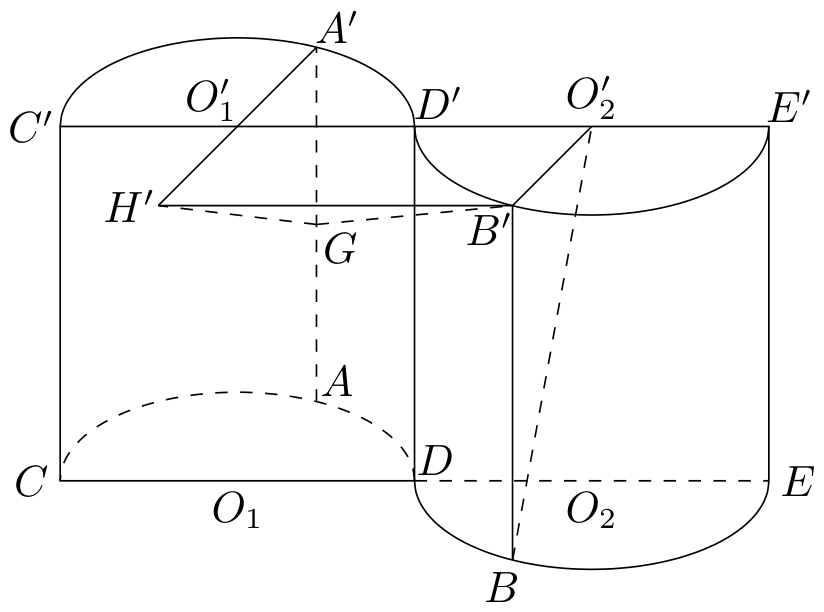
\includegraphics[width=7.8cm]{GaoKao/images/2011/guangdong_liberal/q18_fig1.png}
\end{center}

        \item 设 \(a > 0\)，讨论函数 \(f(x) = \ln x + a(1 - a)x^2 - 2(1 - a)x\) 的单调性.

        \item 设 \(b > 0\)，数列 \(\{a_{n}\}\) 满足 \(a_{1} = b\)，\(a_{n} = \frac{nba_{n - 1}}{a_{n - 1} + n - 1} \)（\(n \geqslant 2\)）.
\begin{enumerate}
\item 求数列 \( \{a_{n}\} \) 的通项公式；
\item 证明：对于一切正整数 \(n\)，\(2a_{n} \leqslant b^{n+1} + 1\).
\end{enumerate}

        \item 在平面直角坐标系 \(xOy\) 中，直线 \(l: x = -2\) 交 \(x\) 轴于点 \(A\). 设 \(P\) 是 \(l\) 上一点，\(M\) 是线段 \(OP\) 的垂直平分线上一点，且满足 \(\angle MPO = \angle AOP\).
\begin{enumerate}
\item 当点 \(P\) 在 \(l\) 上运动时，求点 \(M\) 的轨迹 \(E\) 的方程；
\item 已知 \(T(1,-1)\)，设 \(H\) 是 \(E\) 上动点，求 \( |HO| + |HT| \) 的最小值，并给出此时点 \(H\) 的坐标；
\item 过点 \(T(1, -1)\) 且不平行于 \(y\) 轴的直线 \(l_{1}\) 与轨迹 E 有且只有两个不同的交点，求直线 \(l_{1}\) 的斜率 \(k\) 的取值范围.
\end{enumerate}

    \end{enumerate}

\end{description}


\subsection{2011年湖北卷（理）}\label{gk:2011年湖北卷（理）}

\begin{description}

    \item[一、选择题]

    \begin{enumerate}[leftmargin=5pt]

        \item \(\i\) 为虚数单位，则 \( \left(\frac{1+\i}{1-\i}\right)^{2011}= \)（\quad）

        {\centering\begin{tabular*}{\linewidth}{@{}@{\extracolsep{\fill}}llll@{}}
          \text{A. }\(-\i\)  &  \text{B. }\(-1\)  &  \text{C. }\(\i\)  &  \text{D. }\(1\)
        \end{tabular*}\par}

        \item 已知 \(U = \{y \mid y = \log_2 x, x > 1\}\)，\(P = \left\{y \mid y = \frac{1}{x}, x > 2\right\}\)，则 \(\complement_U P =\)（\quad）

        {\centering\begin{tabular*}{\linewidth}{@{}@{\extracolsep{\fill}}llll@{}}
          \text{A. }\(\left[\frac{1}{2}, +\infty\right)\)  &  \text{B. }\(\left(0, \frac{1}{2}\right)\)  &  \text{C. }\((0, +\infty)\)  &  \text{D. }\((- \infty, 0) \cup \left[\frac{1}{2}, +\infty\right)\)
        \end{tabular*}\par}

        \item 已知函数 \(f(x) = \sqrt{3}\sin x - \cos x\)，\(x \in \mathbb{R}\). 若 \( f(x) \geqslant 1 \)，则 \( x \) 的取值范围为（\quad）

        {\centering\begin{tabular*}{\linewidth}{@{}@{\extracolsep{\fill}}llll@{}}
          \text{A. }\(\left\{x\mid k\pi +\frac{\pi}{3}\leqslant x\leqslant k\pi +\pi ,k\in \mathbb{Z}\right\}\)  &  \text{B. }\(\left\{x\mid 2k\pi +\frac{\pi}{3}\leqslant x\leqslant 2k\pi +\pi ,k\in \mathbb{Z}\right\}\)  &  \text{C. }\(\left\{x\mid k\pi +\frac{\pi}{6}\leqslant x\leqslant k\pi +\frac{5\pi}{6},k\in \mathbb{Z}\right\}\)  &  \text{D. }\(\left\{x\mid 2k\pi +\frac{\pi}{6}\leqslant x\leqslant 2k\pi +\frac{5\pi}{6},k\in \mathbb{Z}\right\}\)
        \end{tabular*}\par}

        \item 将两个顶点在抛物线 \( y^{2} = 2px  \) （\(p > 0\)）上，另一个顶点是此抛物线焦点的正三角形个数记为 \(n\)，则（\quad）

        {\centering\begin{tabular*}{\linewidth}{@{}@{\extracolsep{\fill}}llll@{}}
          \text{A. }\(n = 0\)  &  \text{B. }\(n = 1\)  &  \text{C. }\(n = 2\)  &  \text{D. }\(n \geqslant 3\)
        \end{tabular*}\par}

        \item 已知随机变量 \(\xi\) 服从正态分布 \(N(2, \sigma^2)\)，且 \(P(\xi < 4) = 0.8\)，则 \(P(0 < \xi < 2) =\)（\quad）

        {\centering\begin{tabular*}{\linewidth}{@{}@{\extracolsep{\fill}}llll@{}}
          \text{A. }\(0.6\)  &  \text{B. }\(0.4\)  &  \text{C. }\(0.3\)  &  \text{D. }\(0.2\)
        \end{tabular*}\par}

        \item 已知定义在 \(\mathbb{R}\) 上的奇函数 \(f(x)\) 和偶函数 \(g(x)\) 满足 \(f(x) + g(x) = a^x - a^{-x} + 2\)（\(a > 0\)，且 \(a \neq 1\)）. 若 \(g(2) = a\)，则 \(f(2) =\)（\quad）

        {\centering\begin{tabular*}{\linewidth}{@{}@{\extracolsep{\fill}}llll@{}}
          \text{A. }\(2\)  &  \text{B. }\(\frac{15}{4}\)  &  \text{C. }\(\frac{17}{4}\)  &  \text{D. }\(a^2\)
        \end{tabular*}\par}

        \item 如图，用 \(K\)，\(A_{1}\)，\(A_{2}\) 三类不同的元件连接成一个系统. 当 \(K\) 正常工作且 \(A_{1}\)，\(A_{2}\) 至少有一个正常工作时，系统正常工作. 已知 \(K\)，\(A_{1}\)，\(A_{2}\) 正常工作的概率依次为 0.9，0.8，0.8，则系统正常工作的概率为（\quad）

\begin{center}
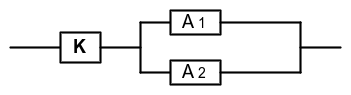
\includegraphics[width=9.3cm]{GaoKao/images/2011/hubei_science/q7_fig1.png}
\end{center}

        {\centering\begin{tabular*}{\linewidth}{@{}@{\extracolsep{\fill}}llll@{}}
          \text{A. }\(0.960\)  &  \text{B. }\(0.864\)  &  \text{C. }\(0.720\)  &  \text{D. }\(0.576\)
        \end{tabular*}\par}

        \item 已知向量 \(\bm{a} = (x + z, 3)\)，\(\bm{b} = (2, y - z)\)，且 \(\bm{a} \perp \bm{b}\). 若 \(x\)，\(y\) 满足不等式 \(|x| + |y| \leqslant 1\)，则 \(z\) 的取值范围为（\quad）

        {\centering\begin{tabular*}{\linewidth}{@{}@{\extracolsep{\fill}}llll@{}}
          \text{A. }\([-2, 2]\)  &  \text{B. }\([-2,3]\)  &  \text{C. }\([-3,2]\)  &  \text{D. }\([-3,3]\)
        \end{tabular*}\par}

        \item 若实数 \(a\)，\(b\) 满足 \(a \geqslant 0\)，\(b \geqslant 0\)，且 \(ab = 0\)，则称 \(a\) 与 \(b\) 互补. 记 \(\varphi(a, b) = \sqrt{a^2 + b^2} - a - b\)，那么 \(\varphi(a, b) = 0\) 是 \(a\) 与 \(b\) 互补的（\quad）

        {\centering\begin{tabular*}{\linewidth}{@{}@{\extracolsep{\fill}}llll@{}}
          \text{A. }必要而不充分条件  &  \text{B. }充分而不必要条件  &  \text{C. }充要条件  &  \text{D. }既不充分也不必要条件
        \end{tabular*}\par}

        \item 放射性元素由于不断有原子放射出微粒子而变成其他元素，其含量不断减少，这种现象称为衰变. 假设在放射性同位素铯 137 的衰变过程中，其含量 \(M\)（单位：太贝克）与时间 \(t\)（单位：年）满足函数关系：\(M(t) = M_0 2^{-t/30}\)，其中 \(M_0\) 为 \(t = 0\) 时铯 137 的含量. 已知 \(t = 30\) 时，铯 137 含量的变化率是 \(-10 \ln 2\)（太贝克/年），则 \(M(60) =\)（\quad）

        {\centering\begin{tabular*}{\linewidth}{@{}@{\extracolsep{\fill}}llll@{}}
          \text{A. }\(5\text{ 太贝克}\)  &  \text{B. }\(75 \ln 2\text{ 太贝克}\)  &  \text{C. }\(150 \ln 2\text{ 太贝克}\)  &  \text{D. }\(150\text{ 太贝克}\)
        \end{tabular*}\par}

    \end{enumerate}

\end{description}

\begin{description}

    \item[二、填空题]

    \begin{enumerate}[leftmargin=5pt]

      \addtocounter{enumi}{+10}

        \item \(\left(x - \frac{1}{3\sqrt{x}}\right)^{18}\) 的展开式中含 \(x^{15}\) 的项的系数为\rule[-0.3ex]{3em}{0.4pt}.（结果用数值表示）

        \item 在 \(30\) 瓶饮料中，有 \(3\) 瓶已过了保质期. 从这 \(30\) 瓶饮料中任取 \(2\) 瓶，则至少取到 \(1\) 瓶已过保质期饮料的概率为\rule[-0.3ex]{3em}{0.4pt}.（结果用最简分数表示）

        \item 《九章算术》“竹九节”问题：现有一根 \(9\) 节的竹子，自上而下各节的容积成等差数列，上面 \(4\) 节的容积共 \(3\text{ 升}\)，下面 \(3\) 节的容积共 \(4\text{ 升}\)，则第 \(5\) 节的容积为\rule[-0.3ex]{3em}{0.4pt}\(\text{升}\).

        \item 如图，直角坐标系 \(xOy\) 所在的平面为 \(\alpha\)，直角坐标系 \(x'Oy'\)（其中 \(y'\) 轴与 \(y\) 轴重合）所在的平面为 \(\beta\)，\(\angle xOx' = 45^\circ\).

\begin{enumerate}
\item 已知平面 \(\beta\) 内有一点 \(P'(2\sqrt{2}, 2)\)，则点 \(P'\) 在平面 \(\alpha\) 内的射影 \(P\) 的坐标为\rule[-0.3ex]{3em}{0.4pt}.
\item 已知平面 \(\beta\) 内的曲线 \(C'\) 的方程是 \(\left(x' - \sqrt{2}\right)^2 + 2y'^2 - 2 = 0\)，则曲线 \(C'\) 在平面 \(\alpha\) 内的射影 \(C\) 的方程是\rule[-0.3ex]{3em}{0.4pt}.
\end{enumerate}

\begin{center}
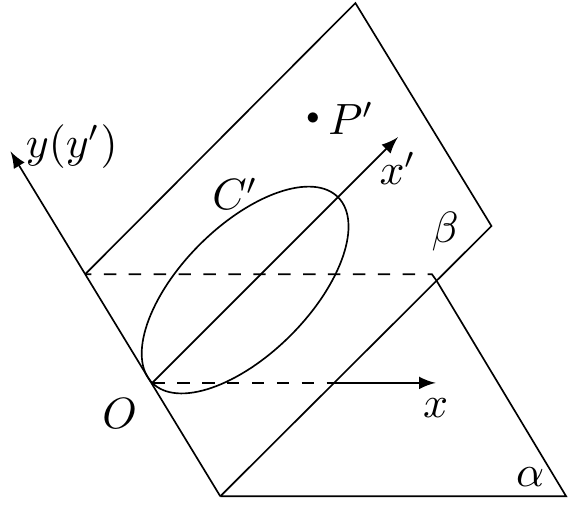
\includegraphics[width=5.4cm]{GaoKao/images/2011/hubei_science/q14_fig1.png}
\end{center}

        \item 给 \(n\) 个自上而下相连的正方形着黑色或白色，当 \(n \leqslant 4\) 时，在所有不同的着色方案中，黑色正方形互不相邻的着色方案如图所示：

由此推断，当 \(n = 6\) 时，黑色正方形互不相邻的着色方案共有\rule[-0.3ex]{3em}{0.4pt} 种，至少有两个黑色正方形相邻的着色方案共有\rule[-0.3ex]{3em}{0.4pt} 种. （结果用数值表示）
{\begin{center}
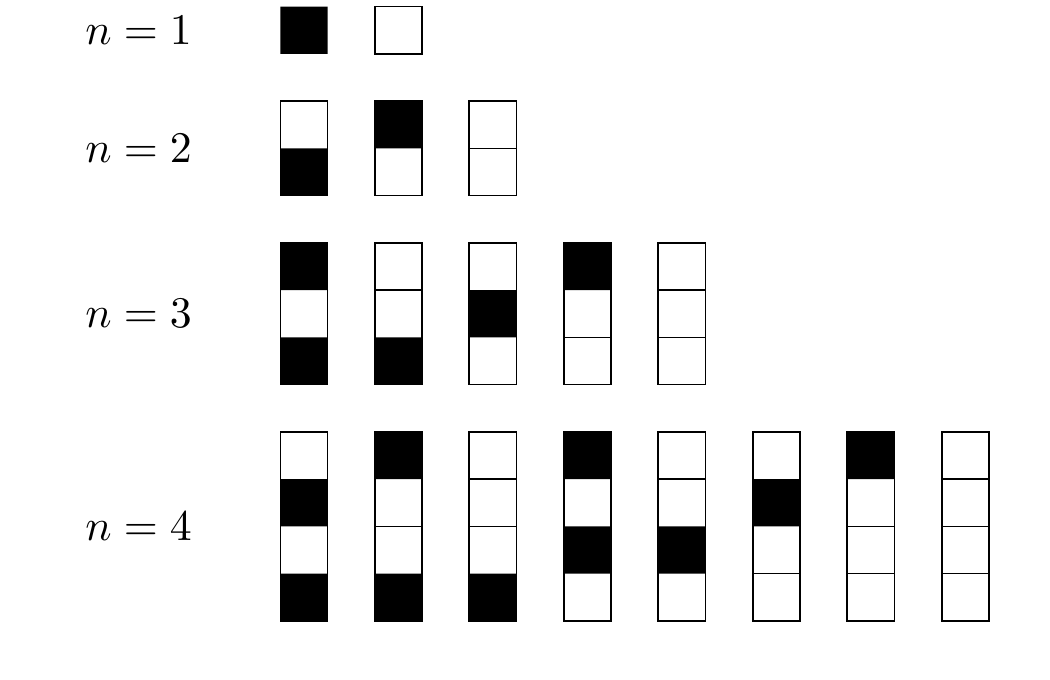
\includegraphics[width=9.0cm]{GaoKao/images/2011/hubei_science/q15_fig1.png}
\end{center}}

    \end{enumerate}

\end{description}

\begin{description}

    \item[三、解答题]

    \begin{enumerate}[leftmargin=5pt]

      \addtocounter{enumi}{+15}

        \item 设 \(\triangle ABC\) 的内角 \(A\)，\(B\)，\(C\) 所对的边分别为 \(a\)，\(b\)，\(c\). 已知 \(a = 1\)，\(b = 2\)，\(\cos C = \frac{1}{4}\).
\begin{enumerate}
\item 求 \( \triangle ABC \) 的周长；
\item 求 \( \cos(A-C) \) 的值.
\end{enumerate}

        \item 提高过江大桥的车辆通行能力可改善整个城市的交通状况. 在一般情况下，大桥上的车流速度 \(v\)（单位：千米/小时）是车流密度 \(x\)（单位：辆/千米）的函数. 当桥上的车流密度达到 \(200\text{ 辆/千米}\) 时，造成堵塞. 此时车流速度为 \(0\)；当车流密度不超过 \(20\text{ 辆/千米}\) 时，车流速度为 \(60\text{ 千米/小时}\)；研究表明：当 \(20 \leqslant x \leqslant 200\) 时，车流速度 \(v\) 是车流密度 \(x\) 的一次函数.
\begin{enumerate}
\item 当 \( 0 \leqslant x \leqslant 200 \) 时，求函数 \( v(x) \) 的表达式；
\item 当车流密度 \(x\) 为多大时，车流量（单位时间内通过桥上某观测点的车辆数，单位：辆/小时）\(f(x) = x \cdot v(x)\) 可以达到最大，并求出最大值.（精确到 \(1\text{ 辆/小时}\)）
\end{enumerate}

        \item 如图，已知正三棱柱 \(ABC - A_{1}B_{1}C_{1}\) 的各棱长都是 \(4\)，\(E\) 是 \(BC\) 的中点，动点 \(F\) 在侧棱 \(CC_{1}\) 上，且不与点 \(C\) 重合.
\begin{enumerate}
\item 当 \(CF=1\) 时，求证：\(EF \perp A_{1}C_{1}\)；
\item 设二面角 \(C - AF - E\) 的大小为 \(\theta\)，求 \(\tan \theta\) 的最小值.
\end{enumerate}

\begin{center}
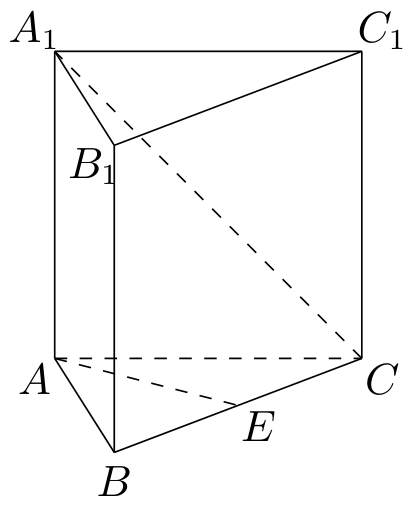
\includegraphics[width=4.2cm]{GaoKao/images/2011/hubei_science/q18_fig1.png}
\end{center}

        \item 已知数列 \(\{a_{n}\}\) 的前 \(n\) 项和为 \(S_{n}\)，且满足 \(a_{1} = a\)，\(a \neq 0\)，\(a_{n+1} = rS_{n}\)，\(n \in \mathbf{N}^{*}\)，\(r \in \mathbb{R}\)，\(r \neq -1\).
\begin{enumerate}
\item 求数列 \( \{a_{n}\} \) 的通项公式；
\item 若存在 \(k \in \mathbf{N}^*\)，使得 \(S_{k+1}\)，\(S_k\)，\(S_{k+2}\) 成等差数列，试判断：对于任意的 \(m \in \mathbf{N}^*\)，且 \(m \geqslant 2\)，\(a_{m+1}\)，\(a_m\)，\(a_{m+2}\) 是否成等差数列，并证明你的结论.
\end{enumerate}

        \item 平面内与两定点 \(A_{1}(-a,0)\)，\(A_{2}(a,0)\)（\(a > 0\)）连线的斜率之积等于非零常数 \(m\) 的点的轨迹. 加上 \(A_{1}\)，\(A_{2}\) 两点所成的曲线 \(C\) 可以是圆，椭圆或双曲线.
\begin{enumerate}
\item 求曲线 \(C\) 的方程，并讨论 \(C\) 的形状与 \(m\) 值的关系；
\item 当 \(m = -1\) 时，对应的曲线为 \(C_1\)；对给定的 \(m \in (-1,0) \cup (0, +\infty)\)，对应的曲线为 \(C_2\). 设 \(F_1\)，\(F_2\) 是 \(C_2\) 的两个焦点. 试问：在 \(C_1\) 上，是否存在点 \(N\)，使得 \(\triangle F_1NF_2\) 的面积 \(S = |m|a^2\)？ 若存在，求 \(\tan \angle F_1NF_2\) 的值；若不存在，请说明理由.
\end{enumerate}

        \item \begin{enumerate}
\item 已知函数 \(f(x) = \ln x - x + 1\)，\(x \in (0, +\infty)\)，求函数 \( f(x) \) 的最大值.

\item 设 \(a_k\)，\(b_k\)（\(k = 1\)，\(2\)，\(\dots\)，\(n\)）均为正数，证明：

\begin{enumerate}
\item 若 \(a_1b_1 + a_2b_2 + \dots + a_nb_n \leqslant b_1 + b_2 + \dots + b_n\)，则 \(a_1^{b_1} a_2^{b_2} \cdots a_n^{b_n} \leqslant 1\)；
\item 若 \(b_{1} + b_{2} + \dots + b_{n} = 1\)，则 \(\frac{1}{n} \leqslant b_{1}^{b_{1}} b_{2}^{b_{2}} \cdots b_{n}^{b_{n}} \leqslant b_{1}^{2} + b_{2}^{2} + \dots + b_{n}^{2}\).
\end{enumerate}
\end{enumerate}

    \end{enumerate}

\end{description}


\subsection{2011年湖北卷（文）}\label{gk:2011年湖北卷（文）}

\begin{description}

    \item[一、选择题]

    \begin{enumerate}[leftmargin=5pt]

        \item 已知 \( U = \{1, 2, 3, 4, 5, 6, 7, 8\} \)， \( A = \{1, 3, 5, 7\} \)， \( B = \{2, 4, 5\} \)，则 \( \complement_{U}(A \cup B) = \)（\quad）

        {\centering\begin{tabular*}{\linewidth}{@{}@{\extracolsep{\fill}}llll@{}}
          \text{A. }\(\{6, 8\}\)  &  \text{B. }\(\{5,7\}\)  &  \text{C. }\( \{4, 6, 7\} \)  &  \text{D. }\(\{1, 3, 5, 6, 8\}\)
        \end{tabular*}\par}

        \item 若向量 \(\bm{a} = (1, 2)\)，\(\bm{b} = (1, -1)\)，则 \(2\bm{a} + \bm{b}\) 与 \(\bm{a} - \bm{b}\) 的夹角等于（\quad）

        {\centering\begin{tabular*}{\linewidth}{@{}@{\extracolsep{\fill}}llll@{}}
          \text{A. }\(-\frac{\pi}{4}\)  &  \text{B. }\( \frac{\pi}{6} \)  &  \text{C. }\( \frac{\pi}{4} \)  &  \text{D. }\(\frac{3\pi}{4}\)
        \end{tabular*}\par}

        \item 若定义在 \(\mathbb{R}\) 上的偶函数 \(f(x)\) 和奇函数 \(g(x)\) 满足 \(f(x) + g(x) = {\mathrm{e}}^{x}\)，则 \(g(x) =\)（\quad）

        {\centering\begin{tabular*}{\linewidth}{@{}@{\extracolsep{\fill}}llll@{}}
          \text{A. }\({\mathrm{e}}^x - {\mathrm{e}}^{-x}\)  &  \text{B. }\(\frac{1}{2} ({\mathrm{e}}^x + {\mathrm{e}}^{-x})\)  &  \text{C. }\(\frac{1}{2} ({\mathrm{e}}^{-x} - {\mathrm{e}}^{x})\)  &  \text{D. }\(\frac{1}{2} ({\mathrm{e}}^{x} - {\mathrm{e}}^{-x})\)
        \end{tabular*}\par}

        \item 将两个顶点在抛物线 \( y^{2} = 2px \)（\(p > 0\)） 上，另一个顶点是此抛物线焦点的正三角形个数记为 \( n \)，则（\quad）

        {\centering\begin{tabular*}{\linewidth}{@{}@{\extracolsep{\fill}}llll@{}}
          \text{A. }\(n = 0\)  &  \text{B. }\(n = 1\)  &  \text{C. }\(n = 2\)  &  \text{D. }\(n \geqslant 3\)
        \end{tabular*}\par}

        \item 有一个容量为 \(200\) 的样本，其频率分布直方图如图所示，根据样本的频率分布直方图估计，样本数据落在区间 \([10,12)\) 内的频数为（\quad）

\begin{center}
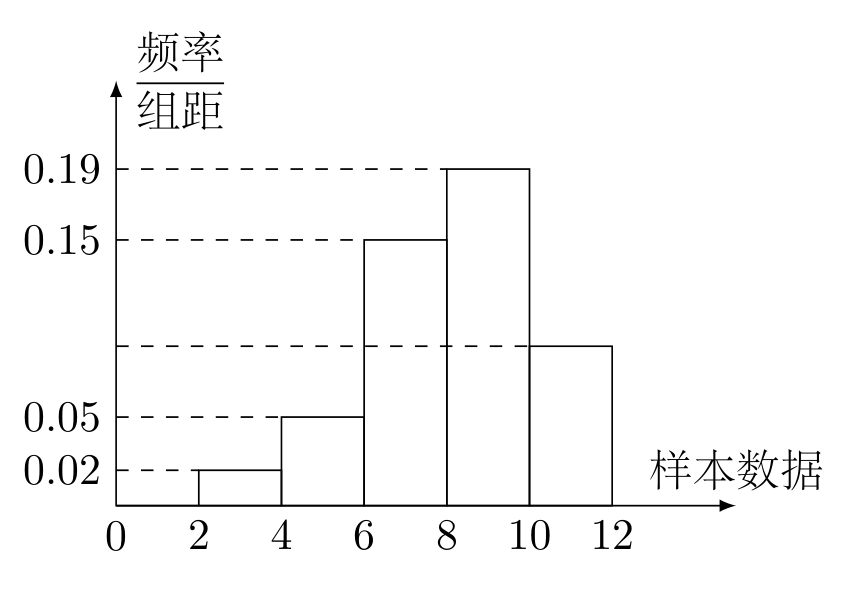
\includegraphics[width=0.42\linewidth]{GaoKao/images/2011/hubei_liberal/q5_fig1.png}
\end{center}

        {\centering\begin{tabular*}{\linewidth}{@{}@{\extracolsep{\fill}}llll@{}}
          \text{A. }\(18\)  &  \text{B. }\(36\)  &  \text{C. }\(54\)  &  \text{D. }\(72\)
        \end{tabular*}\par}

        \item 已知函数 \(f(x) = \sqrt{3}\sin x - \cos x\)，\(x \in \mathbb{R}\). 若 \( f(x) \geqslant 1 \)，则 \( x \) 的取值范围为（\quad）

        {\centering\begin{tabular*}{\linewidth}{@{}@{\extracolsep{\fill}}llll@{}}
          \text{A. }\(\left\{x\mid 2k\pi +\frac{\pi}{3}\leqslant x\leqslant 2k\pi +\pi ,k\in \mathbb{Z}\right\}\)  &  \text{B. }\(\left\{x\mid k\pi +\frac{\pi}{3}\leqslant x\leqslant k\pi +\pi,k\in \mathbb{Z}\right\}\)  &  \text{C. }\(\left\{x\mid 2k\pi +\frac{\pi}{6}\leqslant x\leqslant 2k\pi +\frac{5\pi}{6},k\in \mathbb{Z}\right\}\)  &  \text{D. }\(\left\{x\mid k\pi +\frac{\pi}{6}\leqslant x\leqslant k\pi +\frac{5\pi}{6},k\in \mathbb{Z}\right\}\)
        \end{tabular*}\par}

        \item 设球的体积为 \(V_{1}\). 它的内接正方体的体积为 \(V_{2}\). 下列说法中最合适的是（\quad）

        {\centering\begin{tabular*}{\linewidth}{@{}@{\extracolsep{\fill}}llll@{}}
          \text{A. }\(V_{1}\) 比 \(V_{2}\) 大约多一半  &  \text{B. }\(V_{1}\) 比 \(V_{2}\) 大约多两倍半  &  \text{C. }\(V_{1}\) 比 \(V_{2}\) 大约多一倍  &  \text{D. }\(V_{1}\) 比 \(V_{2}\) 大约多一倍半
        \end{tabular*}\par}

        \item 直线 \(2x + y - 10 = 0\) 与不等式组 \(\begin{cases}
x \geqslant 0,\\
y \geqslant 0,\\
x - y \geqslant -2,\\
4x + 3y \leqslant 20
\end{cases}\) 表示的平面区域的公共点有（\quad）

        {\centering\begin{tabular*}{\linewidth}{@{}@{\extracolsep{\fill}}llll@{}}
          \text{A. }\(0\text{ 个}\)  &  \text{B. }\(1\text{ 个}\)  &  \text{C. }\(2\text{ 个}\)  &  \text{D. }无数个
        \end{tabular*}\par}

        \item 《九章算术》“竹九节”问题：现有一根 \(9\) 节的竹子，自上而下各节的容积成等差数列，上面 \(4\) 节的容积共 \(3\text{ 升}\)，下面 \(3\) 节的容积共 \(4\text{ 升}\)，则第 \(5\) 节的容积为（\quad）

        {\centering\begin{tabular*}{\linewidth}{@{}@{\extracolsep{\fill}}llll@{}}
          \text{A. }\(1\text{ 升}\)  &  \text{B. }\(\frac{67}{66}\text{ 升}\)  &  \text{C. }\(\frac{47}{44}\text{ 升}\)  &  \text{D. }\(\frac{37}{33}\text{ 升}\)
        \end{tabular*}\par}

        \item 若实数 \(a\)，\(b\) 满足 \(a \geqslant 0\)，\(b \geqslant 0\)，且 \(ab = 0\)，则称 \(a\) 与 \(b\) 互补. 记 \(\varphi(a, b) = \sqrt{a^2 + b^2} - a - b\)，那么 \(\varphi(a, b) = 0\) 是 \(a\) 与 \(b\) 互补的（\quad）

        {\centering\begin{tabular*}{\linewidth}{@{}@{\extracolsep{\fill}}llll@{}}
          \text{A. }必要而不充分条件  &  \text{B. }充分而不必要条件  &  \text{C. }充要条件  &  \text{D. }既不充分也不必要条件
        \end{tabular*}\par}

    \end{enumerate}

\end{description}

\begin{description}

    \item[二、填空题]

    \begin{enumerate}[leftmargin=5pt]

      \addtocounter{enumi}{+10}

        \item 某市有大型超市 \(200\text{ 家}\)，中型超市 \(400\text{ 家}\)，小型超市 \(1400\text{ 家}\). 为掌握各类超市的营业情况，现按分层抽样方法抽取一个容量为 \(100\) 的样本，应抽取中型超市\rule[-0.3ex]{3em}{0.4pt} 家.

        \item \(\left(x - \frac{1}{3\sqrt{x}}\right)^{18}\) 的展开式中含 \(x^{15}\) 的项的系数为\rule[-0.3ex]{3em}{0.4pt}. （结果用数值表示）

        \item 在 \(30\) 瓶饮料中，有 \(3\) 瓶已过了保质期. 从这 \(30\) 瓶饮料中任取 \(2\) 瓶，则至少取到 \(1\) 瓶已过保质期饮料的概率为\rule[-0.3ex]{3em}{0.4pt}. （结果用最简分数表示）

        \item 过点 \((-1, -2)\) 的直线 \(t\) 被圆 \(x^{2} + y^{2} - 2x - 2y + 1 = 0\) 截得的弦长为 \(\sqrt{2}\)，则直线 \(t\) 的斜率为\rule[-0.3ex]{3em}{0.4pt}.

        \item 里氏震级 \(M\) 的计算公式为： \(M = \lg A - \lg A_0\). 其中 \(A\) 是测震仪记录的地震曲线的最大振幅，\(A_0\) 是相应的标准地震的振幅. 假设在一次地震中，测震仪记录的最大振幅是 \(1000\)，此时标准地震的振幅为 \(0.001\)，则此次地震的震级为\rule[-0.3ex]{3em}{0.4pt}\(\text{级}\)；\(9\text{ 级}\)地震的最大的振幅是 \(5\text{ 级}\)地震最大振幅的\rule[-0.3ex]{3em}{0.4pt}\(\text{倍}\).

    \end{enumerate}

\end{description}

\begin{description}

    \item[三、解答题]

    \begin{enumerate}[leftmargin=5pt]

      \addtocounter{enumi}{+15}

        \item 设 \(\triangle ABC\) 的内角 \(A\)，\(B\)，\(C\) 所对的边分别为 \(a\)，\(b\)，\(c\). 已知 \(a = 1\)，\(b = 2\)，\(\cos C = \frac{1}{4}\).
\begin{enumerate}
\item 求 \( \triangle ABC \) 的周长；
\item 求 \( \cos(A-C) \) 的值.
\end{enumerate}

        \item 成等差数列的三个正数的和等于 \(15\)，并且这三个数分别加上 \(2\)，\(5\)，\(13\) 后成为等比数列 \(\{b_n\}\) 中的 \(b_3\)，\(b_4\)，\(b_5\).
\begin{enumerate}
\item 求数列 \( \{b_{n}\} \) 的通项公式；
\item 数列 \( \{b_{n}\} \) 的前 \(n\) 项和为 \( S_{n} \)，求证：数列 \( \left\{S_{n}+\frac{5}{4}\right\} \) 是等比数列.
\end{enumerate}

        \item 如图，已知正三棱柱 \(ABC - A_{1}B_{1}C_{1}\) 的底面边长为 \(2\)，侧棱长为 \(3\sqrt{2}\)，点 \(E\) 在侧棱 \(AA_{1}\) 上，点 \(F\) 在侧棱 \(BB_{1}\) 上，且 \(AE = 2\sqrt{2}\)，\(BF = \sqrt{2}\).

\begin{enumerate}
\item 求证：\(CF \perp C_{1}E\).
\item 求二面角 \(E - CF - C_1\) 的大小.
\end{enumerate}

\begin{center}
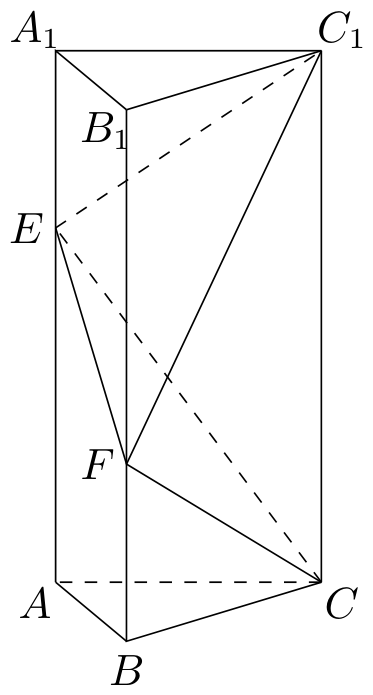
\includegraphics[width=3.7cm]{GaoKao/images/2011/hubei_liberal/q18_fig1.png}
\end{center}

        \item 提高过江大桥的车辆通行能力可改善整个城市的交通状况. 在一般情况下，大桥上的车流速度 \(v\)（单位：千米/小时）是车流密度 \(x\)（单位：辆/千米）的函数. 当桥上的车流密度达到 \(200\text{ 辆/千米}\) 时，造成堵塞，此时车流速度为 \(0\)；当车流密度不超过 \(20\text{ 辆/千米}\) 时，车流速度为 \(60\text{ 千米/小时}\). 研究表明：当 \(20 \leqslant x \leqslant 200\) 时，车流速度 \(v\) 是车流密度 \(x\) 的一次函数.
\begin{enumerate}
\item 当 \(0 \leqslant x \leqslant 200\) 时，求函数 \(v(x)\) 的表达式；
\item 当车流密度 \(x\) 为多大时，车流量（单位时间内通过桥上某观测点的车辆数，单位：辆/小时）\(f(x) = x \cdot v(x)\) 可以达到最大，并求出最大值. （精确到 \(1\text{ 辆/小时}\)）
\end{enumerate}

        \item 设函数 \( f(x) = x^{3} + 2ax^{2} + bx + a \)，\( g(x) = x^{2} - 3x + 2 \)，其中 \( x \in \mathbb{R} \)，\(a\)，\(b\) 为常数，已知曲线 \( y = f(x) \) 与 \( y = g(x) \) 在点 \((2,0)\) 处有相同的切线 \( l \).
\begin{enumerate}
\item 求 \(a\)，\(b\) 的值，并写出切线 \(l\) 的方程；
\item 若方程 \( f(x) + g(x) = mx \) 有三个互不相同的实根 \(0\)，\(x_1\)，\(x_2\)，其中 \( x_1 < x_2 \)，且对任意的 \( x \in [x_1, x_2] \)，\( f(x) + g(x) < m (x - 1) \) 恒成立，求实数 \( m \) 的取值范围.
\end{enumerate}

        \item 平面内与两定点 \(A_{1}(-a,0)\)，\(A_{2}(a,0) \)（\(a > 0\)） 连线的斜率之积等于非零常数 \(m\) 的点的轨迹，加上 \(A_{1}\)，\(A_{2}\) 两点所成的曲线 \(C\) 可以是圆，椭圆或双曲线.
\begin{enumerate}
\item 求曲线 C 的方程，并讨论 C 的形状与 m 值的关系；
\item 当 \(m = -1\) 时，对应的曲线为 \(C_1\)；对给定的 \(m \in (-1,0) \cup (0,+\infty)\)，对应的曲线为 \(C_2\). 设 \(F_1\)，\(F_2\) 是 \(C_2\) 的两个焦点. 试问：在 \(C_1\) 上，是否存在点 \(N\)，使得 \(\triangle F_1NF_2\) 的面积 \(S = |m|a^2\)？若存在，求 \(\tan \angle F_1NF_2\) 的值；若不存在，请说明理由.
\end{enumerate}

    \end{enumerate}

\end{description}


\subsection{2011年湖南卷（理）}\label{gk:2011年湖南卷（理）}

\begin{description}

    \item[一、选择题]

    \begin{enumerate}[leftmargin=5pt]

        \item 若 \(a,b \in \mathbb{R}\)，\(\i\) 为虚数单位，且 \((a + \i)\i = b + \i\)，则（\quad）

        {\centering\begin{tabular*}{\linewidth}{@{}@{\extracolsep{\fill}}llll@{}}
          \text{A. }\(a = 1\)，\(b = 1\)  &  \text{B. }\(a = -1\)，\(b = 1\)  &  \text{C. }\(a = -1\)，\(b = -1\)  &  \text{D. }\(a = 1\)，\(b = -1\)
        \end{tabular*}\par}

        \item 设 \(M = \{1, 2\}\)，\(N = \{a^2\}\)，则 “\(a = 1\)” 是 “\(N \subseteq M\)” 的（\quad）

        {\centering\begin{tabular*}{\linewidth}{@{}@{\extracolsep{\fill}}llll@{}}
          \text{A. }充分不必要条件  &  \text{B. }必要不充分条件  &  \text{C. }充分必要条件  &  \text{D. }既不充分又不必要条件
        \end{tabular*}\par}

        \item 如图是某几何体的三视图，则该几何体的体积为（\quad）

\begin{center}
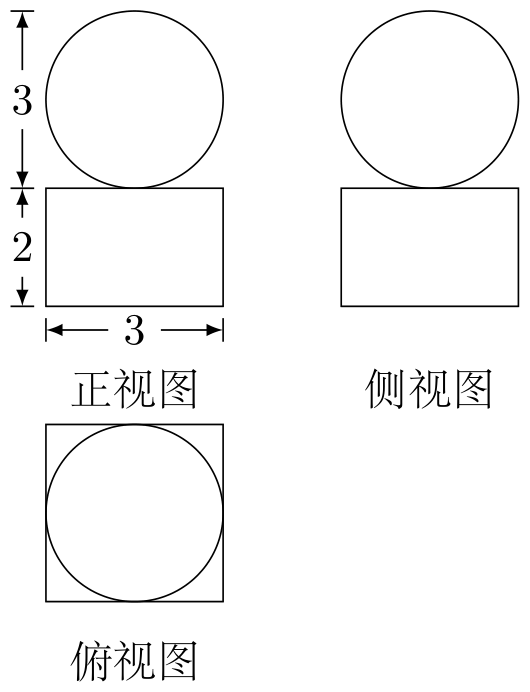
\includegraphics[width=2.1cm]{GaoKao/images/2011/hunan_science/q3_fig1.png}
\end{center}

        {\centering\begin{tabular*}{\linewidth}{@{}@{\extracolsep{\fill}}llll@{}}
          \text{A. }\(\frac{9}{2}\pi + 12\)  &  \text{B. }\(\frac{9}{2}\pi + 18\)  &  \text{C. }\(9\pi + 42\)  &  \text{D. }\(36\pi + 18\)
        \end{tabular*}\par}

        \item 通过随机询问 \(110\text{ 名}\) 性别不同的大学生是否爱好某项运动，得到如下的列联表：

\begin{center}
\begin{tabular}{c|ccc}
 & 男 & 女 & 总计 \\
\hline
爱好 & 40 & 20 & 60 \\
不爱好 & 20 & 30 & 50 \\
总计 & 60 & 50 & 110
\end{tabular}
\end{center}

由 \(K^2 = \frac{n(ad - bc)^2}{(a + b)(c + d)(a + c)(b + d)}\) 算得 \(K^{2} = \frac{110 \times (40 \times 30 - 20 \times 20)^{2}}{60 \times 50 \times 60 \times 50} \approx 7.8\). 附表：

\begin{center}
\begin{tabular}{c|ccc}
\(P(K^2\geqslant k)\) & 0.050 & 0.010 & 0.001 \\
\hline
\(k\) & 3.841 & 6.635 & 10.828
\end{tabular}
\end{center}

参照附表，得到的正确结论是（\quad）

        {\centering\begin{tabular*}{\linewidth}{@{}@{\extracolsep{\fill}}llll@{}}
          \text{A. }在犯错误的概率不超过 \(0.1\%\) 的前提下，认为“爱好该项运动与性别有关”  &  \text{B. }在犯错误的概率不超过 \(0.1\%\) 的前提下，认为“爱好该项运动与性别无关”  &  \text{C. }有 \(99\%\) 以上的把握认为“爱好该项运动与性别有关”  &  \text{D. }有 \(99\%\) 以上的把握认为“爱好该项运动与性别无关”
        \end{tabular*}\par}

        \item 设双曲线 \(\frac{x^2}{a^2} - \frac{y^2}{9} = 1\)（\(a > 0\)）的渐近线方程为 \(3x \pm 2y = 0\)，则 \(a\) 的值为（\quad）

        {\centering\begin{tabular*}{\linewidth}{@{}@{\extracolsep{\fill}}llll@{}}
          \text{A. }4  &  \text{B. }3  &  \text{C. }2  &  \text{D. }1
        \end{tabular*}\par}

        \item 由直线 \(x = -\frac{\pi}{3}\)，\(x = \frac{\pi}{3}\)，\(y = 0\) 与曲线 \(y = \cos x\) 所围成的封闭图形的面积为（\quad）

        {\centering\begin{tabular*}{\linewidth}{@{}@{\extracolsep{\fill}}llll@{}}
          \text{A. }\(\frac{1}{2}\)  &  \text{B. }1  &  \text{C. }\(\frac{\sqrt{3}}{2}\)  &  \text{D. }\(\sqrt{3}\)
        \end{tabular*}\par}

        \item 设 \(m > 1\)，在约束条件 \(\begin{cases}
y \geqslant x,\\
y \leqslant mx,\\
x + y \leqslant 1
\end{cases}\) 下，目标函数 \(z = x + my\) 的最大值小于 \(2\)，则 \(m\) 的取值范围为（\quad）

        {\centering\begin{tabular*}{\linewidth}{@{}@{\extracolsep{\fill}}llll@{}}
          \text{A. }\((1, 1 + \sqrt{2})\)  &  \text{B. }\((1 + \sqrt{2}, +\infty)\)  &  \text{C. }\((1,3)\)  &  \text{D. }\((3, +\infty)\)
        \end{tabular*}\par}

        \item 设直线 \(x = t\) 与函数 \(f(x) = x^2\)，\(g(x) = \ln x\) 的图象分别交于点 \(M\)，\(N\)，则当 \(|MN|\) 达到最小时 \(t\) 的值为（\quad）

        {\centering\begin{tabular*}{\linewidth}{@{}@{\extracolsep{\fill}}llll@{}}
          \text{A. }1  &  \text{B. }\( \frac{1}{2} \)  &  \text{C. }\(\frac{\sqrt{5}}{2}\)  &  \text{D. }\(\frac{\sqrt{2}}{2}\)
        \end{tabular*}\par}

    \end{enumerate}

\end{description}

\begin{description}

    \item[二、填空题]

    \begin{enumerate}[leftmargin=5pt]

      \addtocounter{enumi}{+8}

        \item 在直角坐标系 \(xOy\) 中，曲线 \(C_1\) 的参数方程为 \(\begin{cases}
x = \cos \alpha,\\
y = 1 + \sin \alpha
\end{cases}\) （\(\alpha\) 为参数），在极坐标系（与直角坐标系 \(xOy\) 取相同的长度单位，且以原点 \(O\) 为极点，以 \(x\) 轴正半轴为极轴）中，曲线 \(C_2\) 的方程为 \(\rho (\cos \theta - \sin \theta) + 1 = 0\)，则 \(C_1\) 与 \(C_2\) 的交点个数为\rule[-0.3ex]{3em}{0.4pt}.

        \item 设 \(x,y \in \mathbb{R}\)，且 \(xy \neq 0\)，则 \(\left(x^2 + \frac{1}{y^2}\right)\left(\frac{1}{x^2} + 4y^2\right)\) 的最小值为\rule[-0.3ex]{3em}{0.4pt}.

        \item 如图，\(A\)，\(E\) 是半圆周上的两个三等分点，直径 \(BC=4\)，\(AD\perp BC\)，垂足为 \(D\)，\(BE\) 与 \(AD\) 相交于点 \(F\)，则 \(AF\) 的长为\rule[-0.3ex]{3em}{0.4pt}.

\begin{center}
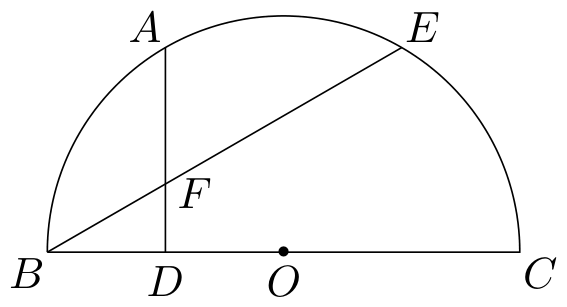
\includegraphics[width=7.0cm]{GaoKao/images/2011/hunan_science/q11_fig1.png}
\end{center}

        \item 设 \(S_{n}\) 是等差数列 \(\{a_{n}\}\)（\(n \in \mathbf{N}^{*}\)）的前 \(n\) 项和，且 \(a_{1} = 1\)，\(a_{4} = 7\)，则 \(S_{5} =\)\rule[-0.3ex]{3em}{0.4pt}.

        \item 若执行如图所示的框图，输入 \(x_{1} = 1\)，\(x_{2} = 2\)，\(x_{3} = 3\)，\(\overline{x} = 2\)，则输出的数等于\rule[-0.3ex]{3em}{0.4pt}.

\begin{center}
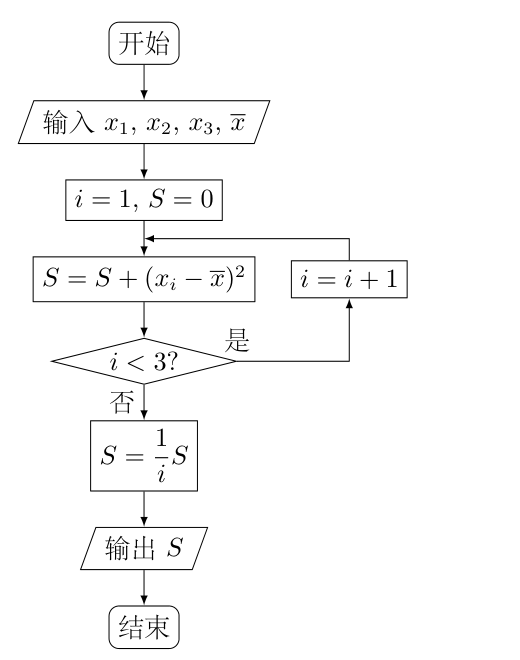
\includegraphics[width=0.32\linewidth]{GaoKao/images/2011/hunan_science/q13_fig1.png}
\end{center}

        \item 在边长为 1 的正三角形 \(ABC\) 中，设 \(\overrightarrow{BC} = 2\overrightarrow{BD}\)，\(\overrightarrow{CA} = 3\overrightarrow{CE}\)，则 \(\overrightarrow{AD} \cdot \overrightarrow{BE} =\)\rule[-0.3ex]{3em}{0.4pt}.

        \item 如图所示，\(EFGH\) 是以 \(O\) 为圆心，半径为 1 的圆的内接正方形，将一颗豆子随机地扔到该圆内，用 \(A\) 表示事件“豆子落在正方形 \(EFGH\) 内”，\(B\) 表示事件“豆子落在扇形 \(OHE\)（阴影部分）内”，则
\begin{enumerate}
\item \(P(A)=\)\rule[-0.3ex]{3em}{0.4pt}；
\item \(P(B|A)=\)\rule[-0.3ex]{3em}{0.4pt}.
\end{enumerate}

\begin{center}
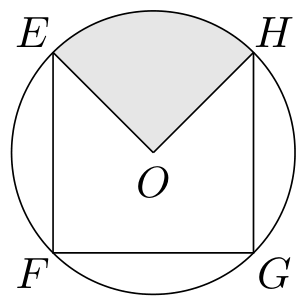
\includegraphics[width=3.7cm]{GaoKao/images/2011/hunan_science/q15_fig1.png}
\end{center}

        \item 对于 \(n \in \mathbf{N}^*\)，将 \(n\) 表示为 \(n = a_0 \times 2^k + a_1 \times 2^{k-1} + a_2 \times 2^{k-2} + \cdots + a_{k-1} \times 2^1 + a_k \times 2^0\). 当 \(i = 0\) 时，\(a_i = 1\)，当 \(1 \leqslant i \leqslant k\) 时，\(a_i\) 为 0 或 1. 记 \(I(n)\) 为上述表示中 \(a_i\) 为 0 的个数 （例如： \(1 = 1 \times 2^0\)，\(4 = 1 \times 2^2 + 0 \times 2^1 + 0 \times 2^0\)，则 \(I(1) = 0\)，\(I(4) = 2\)），则
\begin{enumerate}
    \item \(I(12) =\)\rule[-0.3ex]{3em}{0.4pt}；
    \item \(\displaystyle\sum_{n=1}^{127} 2^{I(n)}=\)\rule[-0.3ex]{3em}{0.4pt}.
\end{enumerate}

    \end{enumerate}

\end{description}

\begin{description}

    \item[三、解答题]

    \begin{enumerate}[leftmargin=5pt]

      \addtocounter{enumi}{+16}

        \item 在 \(\triangle ABC\) 中，角 \(A\)，\(B\)，\(C\) 所对的边分别为 \(a\)，\(b\)，\(c\). 且满足 \(c \sin A = a \cos C\).
\begin{enumerate}
\item 求角 \(C\) 的大小；
\item 求 \(\sqrt{3} \sin A - \cos \left(B + \frac{\pi}{4}\right)\) 的最大值，并求取得最大值时角 A，B 的大小.
\end{enumerate}

        \item 某商店试销某种商品 \(20\text{ 天}\)，获得如下数据：

\begin{center}
\begin{tabular}{c|cccc}
日销售量（件） & 0 & 1 & 2 & 3 \\
\hline
频数 & 1 & 5 & 9 & 5
\end{tabular}
\end{center}

试销结束后（假设该商品的日销售量的分布规律不变），设某天开始营业时有该商品 \(3\text{ 件}\)，当天营业结束后检查存货，若发现存货少于 \(2\text{ 件}\)，则当天进货补充至 \(3\text{ 件}\)，否则不进货，将频率视为概率.

\begin{enumerate}
\item 求当天商品不进货的概率；
\item 记 \(X\) 为第二天开始营业时该商品的件数，求 \(X\) 的分布列和数学期望.
\end{enumerate}

        \item 如图，在圆锥 \(PO\) 中，已知 \(PO = \sqrt{2}\)，\(\odot O\) 的直径 \(AB = 2\)，\(C\) 是 \(\widehat{AB}\) 的中点，\(D\) 为 \(AC\) 的中点.
\begin{enumerate}
\item 证明：平面 \(POD \perp\) 平面 \(PAC\)；
\item 求二面角 \(B - PA - C\) 的余弦值.
\end{enumerate}

\begin{center}
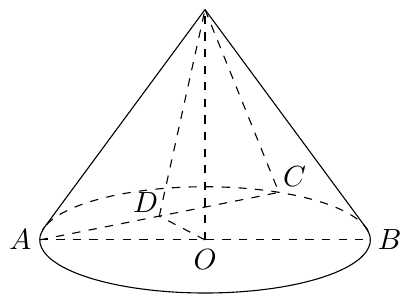
\includegraphics[width=6.9cm]{GaoKao/images/2011/hunan_science/q19_fig1.png}
\end{center}

        \item 如图，长方体物体 \(E\) 在雨中沿面 \(P\)（面积为 \(S\)）的垂直方向作匀速移动，速度为 \(v\)（\(v > 0\)），雨速沿 \(E\) 移动方向的分速度为 \(c\)（\(c \in \mathbb{R}\)）. \(E\) 移动时单位时间内的淋雨量包括两部分：
\begin{enumerate}
\item \(P\) 或 \(P\) 的平行面 （只有一个面淋雨） 的淋雨量，假设其值与 \(|v - c| \times S\) 成正比，比例系数为 \(\frac{1}{10}\)；
\item 其它面的淋雨量之和，其值为 \(\frac{1}{2}\)；
\end{enumerate}
记 \(y\) 为 \(E\) 移动过程中的总淋雨量，当移动距离 \(d = 100\)，面积 \(S = \frac{3}{2}\) 时.
\begin{enumerate}
\item 写出 \(y\) 的表达式；
\item 设 \(0 < v \leqslant 10\)，\(0 < c \leqslant 5\)，试根据 \(c\) 的不同取值范围，确定移动速度 \(v\)，使 \(y\) 最少.
\end{enumerate}


\begin{center}
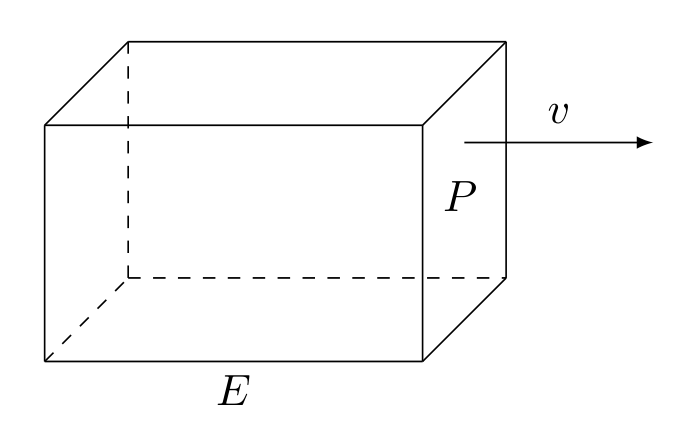
\includegraphics[width=5.3cm]{GaoKao/images/2011/hunan_science/q20_fig1.png}
\end{center}

        \item 如图，椭圆 \(C_{1}:\frac{x^{2}}{a^{2}} +\frac{y^{2}}{b^{2}} = 1\)（\(a > b > 0\)）的离心率为 \(\frac{\sqrt{3}}{2}\)，\(x\) 轴被曲线 \(C_2\)：\(y = x^{2} - b\) 截得的线段长等于 \(C_1\) 的长半轴长.
\begin{enumerate}
\item 求 \(C_1\)，\(C_2\) 的方程；
\item 设 \(C_2\) 与 \(y\) 轴的交点为 \(M\)，过坐标原点 \(O\) 的直线 \(l\) 与 \(C_2\) 相交于点 \(A\)，B，直线 \(MA\)，\(MB\) 分别与 \(C_1\) 相交于点 \(D\)，\(E\).
\begin{enumerate}
\item 证明：\(MD \perp ME\)；
\item 记 \(\triangle MAB\)，\(\triangle MDE\) 的面积分别是 \(S_{1}\)，\(S_{2}\). 问：是否存在直线 \(l\)，使得 \(\frac{S_{1}}{S_{2}} = \frac{17}{32}\)，请说明理由.
\end{enumerate}
\end{enumerate}

\begin{center}
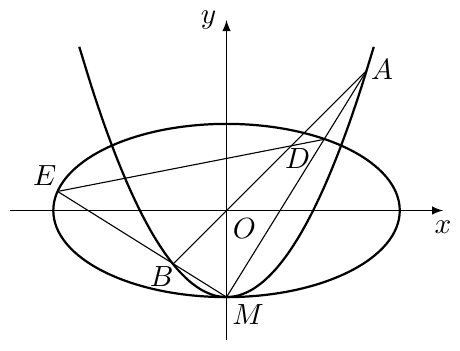
\includegraphics[width=8.6cm]{GaoKao/images/2011/hunan_science/q21_fig1.png}
\end{center}

        \item 已知函数 \(f(x) = x^3\)，\(g(x) = x + \sqrt{x}\).
\begin{enumerate}
\item 求函数 \( h(x) = f(x) - g(x) \) 的零点个数，并说明理由；
\item 设数列 \(\{a_{n}\}\)（\(n \in \mathbf{N}^{*}\)）满足 \(a_{1} = a\)（\(a > 0\)），\(f(a_{n+1}) = g(a_{n})\)，证明：存在常数 \(M\)，使得对于任意的 \(n \in \mathbf{N}^{*}\)，都有 \(a_{n} \leqslant M\).
\end{enumerate}

    \end{enumerate}

\end{description}


\subsection{2011年湖南卷（文）}\label{gk:2011年湖南卷（文）}

\begin{description}

    \item[一、选择题]

    \begin{enumerate}[leftmargin=5pt]

        \item 设全集 \(U = M \cup N = \{1, 2, 3, 4, 5\}\)，\(M \cap \complement_U N = \{2, 4\}\)，则 \(N =\)（\quad）

        {\centering\begin{tabular*}{\linewidth}{@{}@{\extracolsep{\fill}}llll@{}}
          \text{A. }\(\{1, 2, 3\}\)  &  \text{B. }\(\{1,3,5\}\)  &  \text{C. }\(\{1,4,5\}\)  &  \text{D. }\(\{2,3,4\}\)
        \end{tabular*}\par}

        \item 若 \(a,b\in\mathbb{R}\)，\(\i\) 为虚数单位，且 \((a + \i)\i = b + \i\)，则（\quad）

        {\centering\begin{tabular*}{\linewidth}{@{}@{\extracolsep{\fill}}llll@{}}
          \text{A. }\(a = 1\)，\(b = 1\)  &  \text{B. }\(a = -1\)，\(b = 1\)  &  \text{C. }\(a = 1\)，\(b = -1\)  &  \text{D. }\(a = -1\)，\(b = -1\)
        \end{tabular*}\par}

        \item “\(x>1\)”是“\(|x|>1\)”的（\quad）

        {\centering\begin{tabular*}{\linewidth}{@{}@{\extracolsep{\fill}}llll@{}}
          \text{A. }充分不必要条件  &  \text{B. }必要不充分条件  &  \text{C. }充分必要条件  &  \text{D. }既不充分又不必要条件
        \end{tabular*}\par}

        \item 如图是某几何体的三视图，则该几何体的体积为

\begin{center}
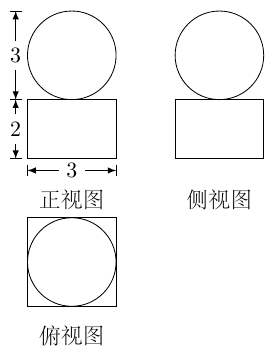
\includegraphics[width=2.2cm]{GaoKao/images/2011/hunan_liberal/q4_fig1.png}
\end{center}

        {\centering\begin{tabular*}{\linewidth}{@{}@{\extracolsep{\fill}}llll@{}}
          \text{A. }\(9\pi + 42\)  &  \text{B. }\(36\pi + 18\)  &  \text{C. }\(\frac{9}{2}\pi + 12\)  &  \text{D. }\(\frac{9}{2}\pi + 18\)
        \end{tabular*}\par}

        \item 通过随机询问 \(110\) 名性别不同的大学生是否爱好某项运动，得到如下的列联表：
\begin{center}
\begin{tabular}{c|ccc}
 & 男 & 女 & 总计 \\
\hline
爱好 & \(40\) & \(20\) & \(60\) \\
不爱好 & \(20\) & \(30\) & \(50\) \\
\hline
总计 & \(60\) & \(50\) & \(110\)
\end{tabular}
\end{center}
由 \(K^2 = \frac{n(ad-bc)^2}{(a + b)(c + d)(a + c)(b + d)}\) 算得，\(K^2 = \frac {110 \times (40 \times 30 - 20 \times 20) ^{2}}{60 \times 50 \times 60 \times 50} \approx 7.8\). 附表：
\begin{center}
\begin{tabular}{c|ccc}
\(P(K^2 \geqslant k)\) & \(0.050\) & \(0.010\) & \(0.001\) \\
\hline
\(k\) & \(3.841\) & \(6.635\) & \(10.828\)
\end{tabular}
\end{center}
参照附表，得到的正确结论是（\quad）

        {\centering\begin{tabular*}{\linewidth}{@{}@{\extracolsep{\fill}}llll@{}}
          \text{A. }有 \(99\%\) 以上的把握认为“爱好该项运动与性别有关”  &  \text{B. }有 \(99\%\) 以上的把握认为“爱好该项运动与性别无关”  &  \text{C. }在犯错误的概率不超过 0.1\% 的前提下，认为“爱好该项运动与性别有关”  &  \text{D. }在犯错误的概率不超过 0.1\% 的前提下，认为“爱好该项运动与性别无关”
        \end{tabular*}\par}

        \item 设双曲线 \(\frac{x^2}{a^2} - \frac{y^2}{9} = 1 \) （\(a > 0\)）的渐近线方程为 \(3x \pm 2y = 0\)，则 \(a\) 的值为（\quad）

        {\centering\begin{tabular*}{\linewidth}{@{}@{\extracolsep{\fill}}llll@{}}
          \text{A. }4  &  \text{B. }3  &  \text{C. }2  &  \text{D. }1
        \end{tabular*}\par}

        \item 曲线 \( y = \frac{\sin x}{\sin x + \cos x} - \frac{1}{2} \) 在点 \( M\left(\frac{\pi}{4}, 0\right) \) 处的切线的斜率为（\quad）

        {\centering\begin{tabular*}{\linewidth}{@{}@{\extracolsep{\fill}}llll@{}}
          \text{A. }\(-\frac{1}{2}\)  &  \text{B. }\( \frac{1}{2} \)  &  \text{C. }\( -\frac{\sqrt{2}}{2} \)  &  \text{D. }\( \frac{\sqrt{2}}{2} \)
        \end{tabular*}\par}

        \item 已知函数 \(f(x) = {\mathrm{e}}^{x} - 1\)，\(g(x) = -x^{2} + 4x - 3\)，若有 \( f(a) = g(b) \)，则 \( b \) 的取值范围为（\quad）

        {\centering\begin{tabular*}{\linewidth}{@{}@{\extracolsep{\fill}}llll@{}}
          \text{A. }\([2 - \sqrt{2}, 2 + \sqrt{2}]\)  &  \text{B. }\((2 - \sqrt{2}, 2 + \sqrt{2})\)  &  \text{C. }\([1,3]\)  &  \text{D. }\((1,3)\)
        \end{tabular*}\par}

    \end{enumerate}

\end{description}

\begin{description}

    \item[二、选做题]

    \begin{enumerate}[leftmargin=5pt]

      \addtocounter{enumi}{+8}

        \item \textbf{【选修4-4：坐标系与参数方程】}

在直角坐标系 \(xOy\) 中，曲线 \(C_1\) 的参数方程为 \(\begin{cases}
x = 2\cos \alpha,\\
y = \sqrt{3}\sin \alpha,
\end{cases}\)（\(\alpha\) 为参数）在极坐标系（与直角坐标系 \(xOy\) 取相同的长度单位，且以原点 \(O\) 为极点，以 \(x\) 轴正半轴为极轴）中，曲线 \(C_2\) 的方程为 \(\rho(\cos \theta - \sin \theta) + 1 = 0\)，则 \(C_1\) 与 \(C_2\) 的交点个数为\rule[-0.3ex]{3em}{0.4pt}.

        \item 已知某试验范围为 \([10,90]\)，若用分数法进行 \(4\) 次优选试验，则第二次试点可以是\rule[-0.3ex]{3em}{0.4pt}.

    \end{enumerate}

\end{description}

\begin{description}

    \item[三、填空题]

    \begin{enumerate}[leftmargin=5pt]

      \addtocounter{enumi}{+10}

        \item 若执行如图所示的框图，输入 \(x_{1} = 1\)，\(x_{2} = 2\)，\(x_{3} = 4\)，\(x_{4} = 8\)，则输出的数等于\rule[-0.3ex]{3em}{0.4pt}.

\begin{center}
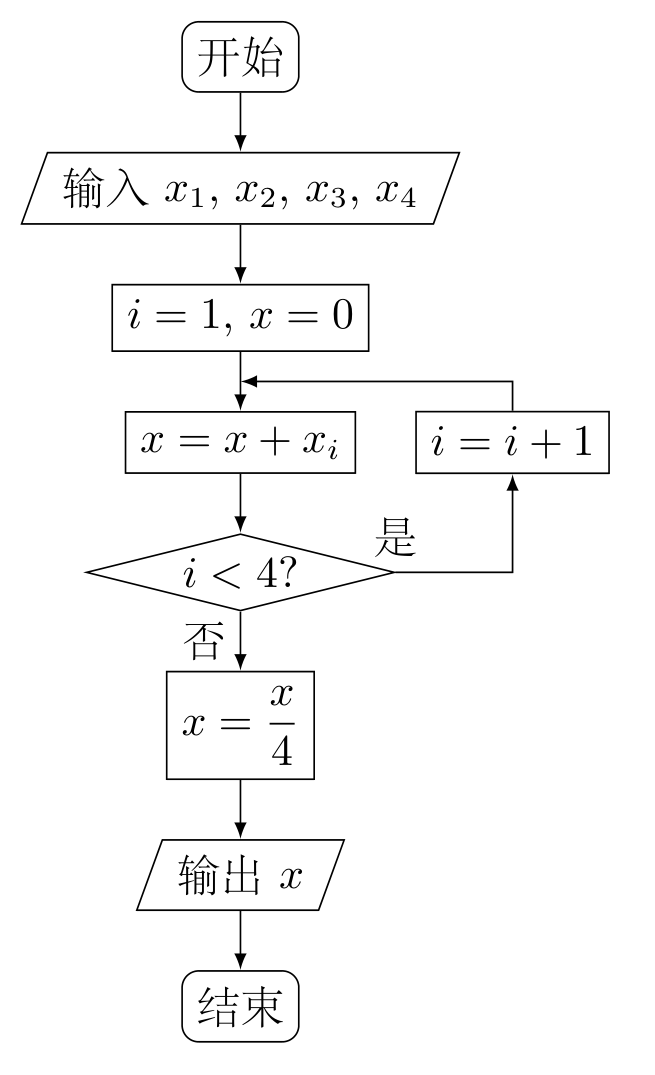
\includegraphics[width=0.30\linewidth]{GaoKao/images/2011/hunan_liberal/q11_fig1.png}
\end{center}

        \item 已知 \( f(x) \) 为奇函数，\( g(x) = f(x) + 9 \)，\( g(-2) = 3 \)，则 \( f(2) = \)\rule[-0.3ex]{3em}{0.4pt}.

        \item 设向量 \(\bm{a}\)，\(\bm{b}\) 满足 \(|\bm{a}| = 2\sqrt{5}\)，\(\bm{b} = (2, 1)\)，且 \(\bm{a}\) 与 \(\bm{b}\) 的方向相反，则 \(\bm{a}\) 的坐标为\rule[-0.3ex]{3em}{0.4pt}.

        \item 设 \(m > 1\)，在约束条件 \(\begin{cases}
y \geqslant x,\\
y \leqslant mx,\\
x + y \leqslant 1
\end{cases}\) 下目标函数 \(z = x + 5y\) 的最大值为 \(4\)，则 \(m\) 的值为\rule[-0.3ex]{3em}{0.4pt}.

        \item 已知圆 \(C: x^{2} + y^{2} = 12\)，直线 \(l: 4x + 3y = 25\).
\begin{enumerate}
\item 圆 \(C\) 的圆心到直线 \(l\) 的距离为\rule[-0.3ex]{3em}{0.4pt}；
\item 圆 \(C\) 上任意一点 \(A\) 到直线 \(l\) 的距离小于 2 的概率为\rule[-0.3ex]{3em}{0.4pt}.
\end{enumerate}

        \item 给定 \(k \in \mathbb{N}^*\)，设函数 \(f: \mathbb{N}^* \to \mathbb{N}^*\) 满足：对于任意大于 \(k\) 的正整数 \(n\)，\(f(n) = n - k\).
\begin{enumerate}
\item 设 \(k = 1\)，则其中一个函数 \(f\) 在 \(n = 1\) 处的函数值为\rule[-0.3ex]{3em}{0.4pt}；
\item 设 \(k = 4\)，且当 \(n \leqslant 4\) 时，\(2 \leqslant f(n) \leqslant 3\)，则不同的函数 \(f\) 的个数为\rule[-0.3ex]{3em}{0.4pt}.
\end{enumerate}

    \end{enumerate}

\end{description}

\begin{description}

    \item[四、解答题]

    \begin{enumerate}[leftmargin=5pt]

      \addtocounter{enumi}{+16}

        \item 在 \(\triangle ABC\) 中，角 \(A\)，\(B\)，\(C\) 所对的边分别为 \(a\)，\(b\)，\(c\)，且满足 \(c \sin A = a \cos C\).
\begin{enumerate}
\item 求角 \(C\) 的大小；
\item 求 \( \sqrt{3}\sin A - \cos\left(B + \frac{\pi}{4}\right) \) 的最大值，并求取得最大值时角 \(A\)，\(B\) 的大小.
\end{enumerate}

        \item 某河流上的一座水力发电站，每年六月份的发电量 \(Y\)（单位：\(\text{万千瓦时}\)）与该河上游在六月份的降雨量 \(X\)（单位：\(\text{毫米}\)）有关，据统计，当 \(X = 70\) 时，\(Y = 460\)；\(X\) 每增加 \(10\)，\(Y\) 增加 \(5\). 已知近 \(20\) 年 \(X\) 的值为：\(140\)，\(110\)，\(160\)，\(70\)，\(200\)，\(160\)，\(140\)，\(160\)，\(220\)，\(200\)，\(110\)，\(160\)，\(160\)，\(200\)，\(140\)，\(110\)，\(160\)，\(220\)，\(140\)，\(160\).

\begin{enumerate}
\item 完成如下的频率分布表：

\begin{center}
\begin{tabular}{c|cccccc}
降雨量 & \(70\) & \(110\) & \(140\) & \(160\) & \(200\) & \(220\) \\
\hline
频率 & \(\frac{1}{20}\) &\rule[-0.3ex]{3em}{0.4pt} & \(\frac{4}{20}\) &\rule[-0.3ex]{3em}{0.4pt} &\rule[-0.3ex]{3em}{0.4pt} & \(\frac{2}{20}\)
\end{tabular}
\end{center}

\item 假定今年六月份的降雨量与近 \(20\) 年六月份降雨量的分布规律相同，并将频率视为概率，求今年六月份该水力发电站的发电量低于 \(490\text{ 万千瓦时}\) 或超过 \(530\text{ 万千瓦时}\) 的概率.
\end{enumerate}

        \item 如图，在圆锥 \(PO\) 中，已知 \(PO = \sqrt{2}\)，\(\odot O\) 的直径 \(AB = 2\)，点 \(C\) 在 \(\widehat{AB}\) 上，且 \(\angle CAB = 30^{\circ}\)，\(D\) 为 \(AC\) 的中点.

\begin{enumerate}
\item 证明： \(AC \perp\) 平面 \(POD\)；
\item 求直线 \(OC\) 和平面 \(PAC\) 所成角的正弦值.
\end{enumerate}

\begin{center}
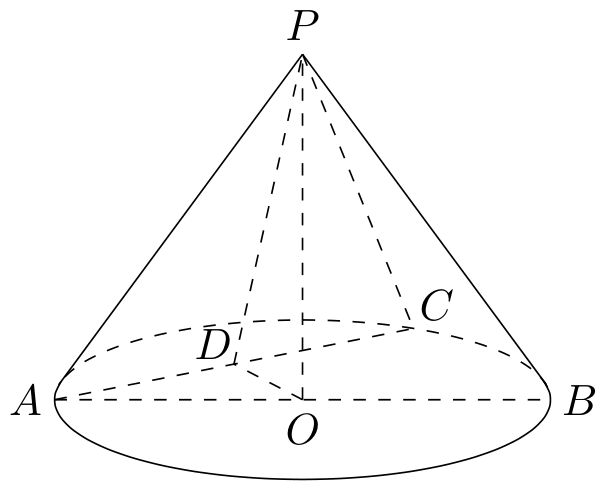
\includegraphics[width=7.0cm]{GaoKao/images/2011/hunan_liberal/q19_fig1.png}
\end{center}

        \item 某企业在第\(1\)年初购买一台价值为 \(120\text{ 万元}\) 的设备 \(M\)，\(M\) 的价值在使用过程中逐年减少. 从第\(2\)年到第\(6\)年，每年初 \(M\) 的价值比上年初减少 \(10\text{ 万元}\)；从第\(7\)年开始，每年初 \(M\) 的价值为上年初的 \(75\%\).
\begin{enumerate}
\item 求第 \(n\) 年初 \(M\) 的价值 \(a_{n}\) 的表达式；
\item 设 \(A_{n} = \frac{a_{1} + a_{2} + \cdots + a_{n}}{n}\)，若 \(A_{n}\) 大于 \(80\text{ 万元}\)，则 \(M\) 继续使用，否则须在第\(n\)年初对 \(M\) 更新，证明：须在第\(9\)年初对 \(M\) 更新.
\end{enumerate}

        \item 已知平面内一动点 \(P\) 到点 \(F(1,0)\) 的距离与点 \(P\) 到 \(y\) 轴的距离的差等于 \(1\).
\begin{enumerate}
\item 求动点 \(P\) 的轨迹 \(C\) 的方程；
\item 过点 \(F\) 作两条斜率存在且互相垂直的直线 \(l_{1}\)，\(l_{2}\)，设 \(l_{1}\) 与轨迹 \(C\) 相交于点 \(A\)，\(B\)，\(l_{2}\) 与轨迹 \(C\) 相交于点 \(D\)，\(E\)，求 \(\overrightarrow{AD} \cdot \overrightarrow{EB}\) 的最小值.
\end{enumerate}

        \item 设函数 \( f(x) = x - \frac{1}{x} - a \ln x  \)（\(a \in \mathbb{R}\)）.
\begin{enumerate}
\item 讨论函数 \( f(x) \) 的单调性.
\item 若 \( f(x) \) 有两个极值点 \( x_{1} \) 和 \( x_{2} \)，记过点 \( A(x_{1}, f(x_{1})) \)，\( B(x_{2}, f(x_{2})) \) 的直线斜率为 \( k \). 问：是否存在 \( a \)，使得 \( k = 2 - a^{2} \)？若存在，求出 \( a \) 的值；若不存在，请说明理由.
\end{enumerate}

    \end{enumerate}

\end{description}


\subsection{2011年江苏卷}\label{gk:2011年江苏卷}

\begin{description}

    \item[一、填空题]

    \begin{enumerate}[leftmargin=5pt]

        \item 已知集合 \(A = \{-1, 1, 2, 4\}\)，\(B = \{-1, 0, 2\}\). 则 \(A \cap B =\rule[-0.3ex]{3em}{0.4pt}.\)

        \item 函数 \(f(x)=\log_{5}(2x+1)\) 的单调增区间是\rule[-0.3ex]{3em}{0.4pt}.

        \item 设复数 \(z\) 满足 \(\i(z+1)=-3+2\i\)（\(\i\) 是虚数单位），则 \(z\) 的实部是\rule[-0.3ex]{3em}{0.4pt}.

        \item 根据如图所示伪代码，当输入 \(a\)，\(b\) 分别为 \(2, 3\) 时，最后输出的 \(m\) 的值是\rule[-0.3ex]{3em}{0.4pt}.

\begin{center}
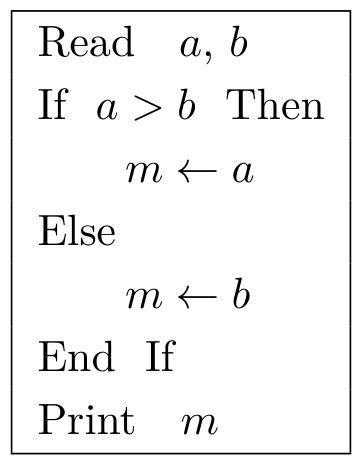
\includegraphics[width=4.3cm]{GaoKao/images/2011/jiangsu/q4_fig1.png}
\end{center}

        \item 从 \(1\)，\(2\)，\(3\)，\(4\) 这四个数中一次随机取两个数，则其中一个数是另一个的两倍的概率是\rule[-0.3ex]{3em}{0.4pt}.

        \item 某老师从星期一到星期五收到信件数分别是 \(10\)，\(6\)，\(8\)，\(5\)，\(6\)，则该组数据的方差 \(s^2=\)\rule[-0.3ex]{3em}{0.4pt}.

        \item 已知 \(\tan\left(x+\frac{\pi}{4}\right)=2\)，则 \(\frac{\tan x}{\tan 2x}\) 的值为\rule[-0.3ex]{3em}{0.4pt}.

        \item 在平面直角坐标系 \(xOy\) 中，过坐标原点的一条直线与函数 \(f(x)=\frac{2}{x}\) 的图象交于 \(P\)，\(Q\) 两点，则线段 \(PQ\) 长的最小值是\rule[-0.3ex]{3em}{0.4pt}.

        \item 函数 \(f(x)=A\sin(\omega x+\varphi)\)（\(A\)，\(\omega\)，\(\varphi\) 是常数，\(A>0\)，\(\omega>0\)）的部分图象如图所示，则 \(f(0)=\)\rule[-0.3ex]{3em}{0.4pt}.

\begin{center}
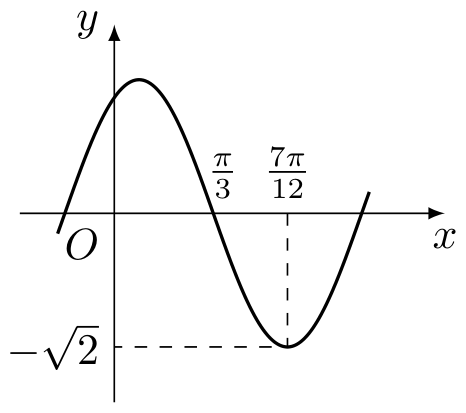
\includegraphics[width=4.8cm]{GaoKao/images/2011/jiangsu/q9_fig1.png}
\end{center}

        \item 已知 \(\bm{e}_1\)，\(\bm{e}_2\) 是夹角为 \(\frac{2\pi}{3}\) 的两个单位向量，\(\bm{a}=\bm{e}_1-2\bm{e}_2\)，\(\bm{b}=k\bm{e}_1+\bm{e}_2\). 若 \(\bm{a}\cdot\bm{b}=0\)，则 \(k\) 的值为\rule[-0.3ex]{3em}{0.4pt}.

        \item 已知实数 \(a\neq 0\)，函数 \(f(x)=\begin{cases}
2x+a, & x<1,\\
-x-2a, & x\geqslant 1.
\end{cases}\)
若 \(f(1-a)=f(1+a)\)，则 \(a\) 的值为\rule[-0.3ex]{3em}{0.4pt}.

        \item 在平面直角坐标系 \(xOy\) 中，已知点 \(P\) 是函数 \(f(x)={\mathrm{e}}^x\) （\(x>0\)）的图象上的动点，该图象在 \(P\) 处的切线 \(l\) 交 \(y\) 轴于点 \(M\). 过点 \(P\) 作 \(l\) 的垂线交 \(y\) 轴于点 \(N\). 设线段 \(MN\) 的中点的纵坐标为 \(t\)，则 \(t\) 的最大值是\rule[-0.3ex]{3em}{0.4pt}.

        \item 设 \(1=a_{1}\leqslant a_{2}\leqslant \cdots \leqslant a_{7}\)，其中 \(a_{1}\)，\(a_{3}\)，\(a_{5}\)，\(a_{7}\) 成公比为 \(q\) 的等比数列，\(a_{2}\)，\(a_{4}\)，\(a_{6}\) 成公差为 \(1\) 的等差数列，则 \(q\) 的最小值是\rule[-0.3ex]{3em}{0.4pt}.

        \item 设集合 \(A=\left\{(x,y)\mid \frac{m}{2}\leqslant (x-2)^2+y^2\leqslant m^2,\ x,y\in\mathbb{R}\right\}\).

集合 \(B=\left\{(x,y)\mid 2m\leqslant x+y\leqslant 2m+1,\ x,y\in\mathbb{R}\right\}\).
若 \(A\cap B\neq\emptyset\)，则实数 \(m\) 的取值范围是\rule[-0.3ex]{3em}{0.4pt}.

    \end{enumerate}

\end{description}

\begin{description}

    \item[二、解答题]

    \begin{enumerate}[leftmargin=5pt]

      \addtocounter{enumi}{+14}

        \item 在 \(\triangle ABC\) 中，角 \(A\)，\(B\)，\(C\) 所对应的边为 \(a\)，\(b\)，\(c\).
\begin{enumerate}
\item 若 \(\sin\left(A+\frac{\pi}{6}\right)=2\cos A\)，求 \(A\) 的值；
\item 若 \(\cos A=\frac{1}{3}\)，\(b=3c\)，求 \(\sin C\) 的值.
\end{enumerate}

        \item 如图，在四棱锥 \(P-ABCD\) 中，平面 \(PAD\perp\) 平面 \(ABCD\)，\(AB=AD\)，\(\angle BAD=60^\circ\)，\(E\)，\(F\) 分别是 \(AP\)，\(AD\) 的中点. 求证：
\begin{enumerate}
\item 直线 \(EF\parallel\) 平面 \(PCD\)；
\item 平面 \(BEF\perp\) 平面 \(PAD\).
\end{enumerate}
\begin{center}
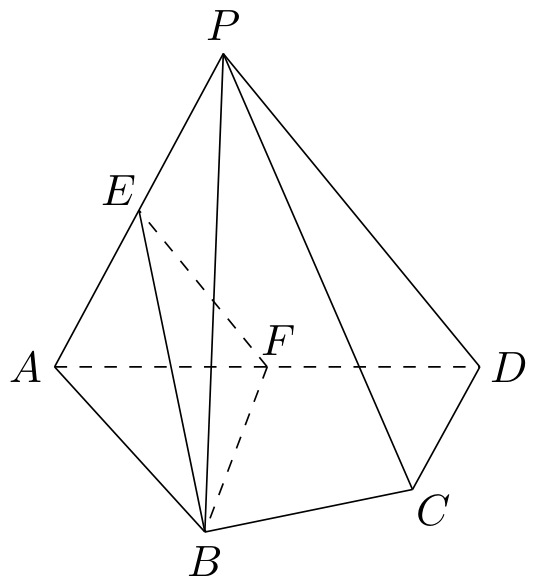
\includegraphics[width=6.7cm]{GaoKao/images/2011/jiangsu/q16_fig1.png}
\end{center}

        \item 请你设计一个包装盒. 如图所示，\(ABCD\) 是边长为 \(60\mathrm{~cm}\) 的正方形硬纸片，切去阴影部分所示的四个全等的等腰直角三角形，再沿虚线折起，使得 \(A\)，\(B\)，\(C\)，\(D\) 四个点重合于图中的点 \(P\)，正好形成一个正四棱柱形状的包装盒，\(E\)，\(F\) 在 \(AB\) 上，是被切去的等腰直角三角形斜边的两个端点. 设 \(AE=FB=x\)（\(\mathrm{cm}\)）.

\begin{enumerate}
\item 若广告商要求包装盒侧面积 \(S\)（\(\mathrm{cm}^2\)）最大，试问 \(x\) 应取何值？
\item 若广告商要求包装盒容积 \(V\)（\(\mathrm{cm}^3\)）最大，试问 \(x\) 应取何值？ 并求出此时包装盒的高与底面边长的比值.
\end{enumerate}
\begin{center}
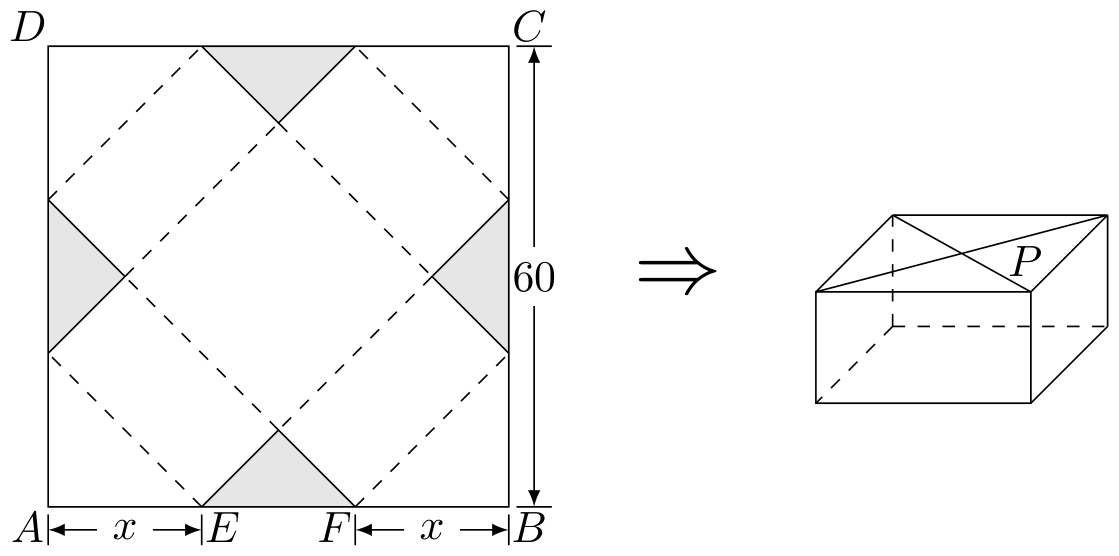
\includegraphics[width=10.9cm]{GaoKao/images/2011/jiangsu/q17_fig1.png}
\end{center}

        \item 如图，在平面直角坐标系 \(xOy\) 中，\(M\)，\(N\) 分别是椭圆 \(\frac{x^2}{4}+\frac{y^2}{2}=1\) 的顶点，过坐标原点的直线交椭圆于 \(P\)，\(A\) 两点，其中点 \(P\) 在第一象限，过 \(P\) 作 \(x\) 轴的垂线，垂足为 \(C\)，连接 \(AC\)，并延长交椭圆于点 \(B\)，设直线 \(PA\) 的斜率为 \(k\).

\begin{enumerate}
\item 当直线 \(PA\) 平分线段 \(MN\) 时，求 \(k\) 的值；
\item 当 \(k=2\) 时，求点 \(P\) 到直线 \(AB\) 的距离 \(d\)；
\item 对任意 \(k>0\)，求证：\(PA\perp PB\).
\end{enumerate}
\begin{center}
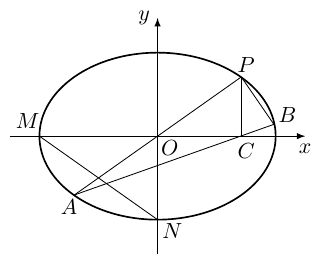
\includegraphics[width=8.0cm]{GaoKao/images/2011/jiangsu/q18_fig1.png}
\end{center}

        \item 已知 \(a\)，\(b\) 是实数，函数 \(f(x)=x^3+ax\)，\(g(x)=x^2+bx\)，\(f'(x)\) 和 \(g'(x)\) 分别是 \(f(x)\)，\(g(x)\) 的导函数，若 \(f'(x)g'(x)\geqslant 0\) 在区间 \(I\) 上恒成立，则称 \(f(x)\) 和 \(g(x)\) 在区间 \(I\) 上单调性一致.

\begin{enumerate}
\item 设 \(a>0\)，若函数 \(f(x)\) 和 \(g(x)\) 在区间 \([-1,+\infty)\) 上单调性一致，求实数 \(b\) 的取值范围；
\item 设 \(a<0\) 且 \(a\neq b\)，若 \(f(x)\) 和 \(g(x)\) 在以 \(a\)，\(b\) 为端点的开区间上单调性一致，求 \(|a-b|\) 的最大值.
\end{enumerate}

        \item 设 \(M\) 为部分正整数组成的集合，数列 \(\{a_{n}\}\) 的首项 \(a_{1}=1\)，前 \(n\) 项和为 \(S_{n}\)，已知对任意整数 \(k\in M\)，当整数 \(n>k\) 时，\(S_{n+k}+S_{n-k}=2(S_{n}+S_{k})\) 都成立.

\begin{enumerate}
\item 设 \(M=\{1\}\)，\(a_{2}=2\)，求 \(a_{5}\) 的值；
\item 设 \(M=\{3,4\}\)，求数列 \(\{a_{n}\}\) 的通项公式.
\end{enumerate}

    \end{enumerate}

\end{description}

\begin{description}

    \item[三、附加题]

    \begin{enumerate}[leftmargin=5pt]

      \addtocounter{enumi}{+20}

        \item [A]
如图，圆 \(O_{1}\) 与圆 \(O_{2}\) 内切于点 \(A\)，其半径分别为 \(r_1\) 与 \(r_2\)（\(r_1>r_2\)），圆 \(O_{1}\) 的弦 \(AB\) 交圆 \(O_{2}\) 于点 \(C\)（\(O_{1}\) 不在 \(AB\) 上），求证：\(AB:AC\) 为定值.

\begin{center}
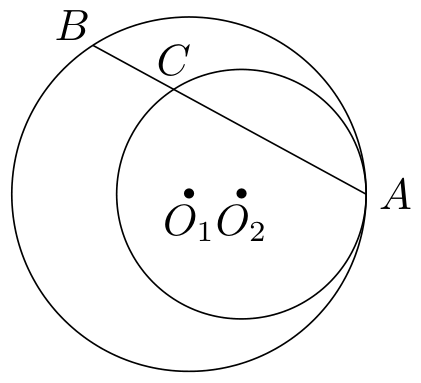
\includegraphics[width=4.9cm]{GaoKao/images/2011/jiangsu/q21_fig1.png}
\end{center}

        \item [B]
已知矩阵 \(A=\begin{bmatrix}1&1\\ 2&1\end{bmatrix}\)，向量 \(\bm{\beta}=\begin{bmatrix}1\\ 2\end{bmatrix}\)，求向量 \(\bm{\alpha}\)，使得 \(A^{2}\bm{\alpha}=\bm{\beta}\).

        \item [C]
在平面直角坐标系 \(xOy\) 中，求过椭圆 \(\begin{cases}
x=5\cos\varphi,\\
y=3\sin\varphi,
\end{cases}\)
（\(\varphi\) 为参数）的右焦点，且与直线 \(\begin{cases}
x=4-2t,\\
y=3-t,
\end{cases}\)
（\(t\) 为参数）平行的直线的普通方程.

        \item [D]
解不等式：\(x+|2x-1|<3\).

        \item 如图，在正四棱柱 \(ABCD-A_{1}B_{1}C_{1}D_{1}\) 中，\(AA_{1}=2\)，\(AB=1\)，点 \(N\) 是 \(BC\) 的中点，点 \(M\) 在 \(CC_{1}\) 上. 设二面角 \(A_{1}-DN-M\) 的大小为 \(\theta\).
\begin{enumerate}
\item 当 \(\theta=90^\circ\) 时，求 \(AM\) 的长；
\item 当 \(\cos\theta=\frac{\sqrt{6}}{6}\) 时，求 \(CM\) 的长.
\end{enumerate}
\begin{center}
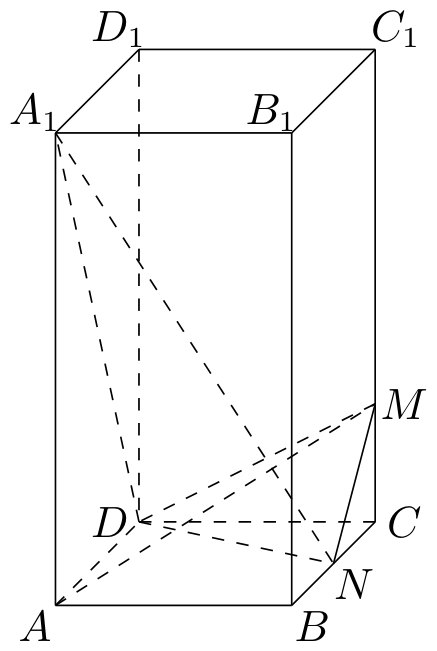
\includegraphics[width=4.4cm]{GaoKao/images/2011/jiangsu/q22_fig1.png}
\end{center}

        \item 设整数 \(n\geqslant 4\)，\(P(a,b)\) 是平面直角坐标系 \(xOy\) 中的点，其中 \(a,b\in\{1,2,3,\dots,n\}\)，\(a>b\).
\begin{enumerate}
\item 记 \(A_{n}\) 为满足 \(a-b=3\) 的点 \(P\) 的个数，求 \(A_{n}\)；
\item 记 \(B_{n}\) 为满足 \(\frac{1}{3}(a-b)\) 是整数的点 \(P\) 的个数，求 \(B_{n}\).
\end{enumerate}

    \end{enumerate}

\end{description}


\subsection{2011年江西卷（理）}\label{gk:2011年江西卷（理）}

\begin{description}

    \item[一、选择题]

    \begin{enumerate}[leftmargin=5pt]

        \item 若 \(z = \frac{1 + 2\i}{\i}\)，则复数 \(z =\)（\quad）

        {\centering\begin{tabular*}{\linewidth}{@{}@{\extracolsep{\fill}}llll@{}}
          \text{A. }\(-2 - \i\)  &  \text{B. }\(-2 + \i\)  &  \text{C. }\(2 - \i\)  &  \text{D. }\(2 + \i\)
        \end{tabular*}\par}

        \item 若集合 \(A = \{x \mid -1 \leqslant 2x + 1 \leqslant 3\}\)，\(B = \left\{x \left| \frac{x - 2}{x} \leqslant 0 \right.\right\}\)，则 \(A \cap B =\)（\quad）

        {\centering\begin{tabular*}{\linewidth}{@{}@{\extracolsep{\fill}}llll@{}}
          \text{A. }\(\{x\mid -1\leqslant x < 0\}\)  &  \text{B. }\(\{x\mid 0 < x\leqslant 1\}\)  &  \text{C. }\(\{x\mid 0\leqslant x\leqslant 2\}\)  &  \text{D. }\(\{x\mid 0\leqslant x\leqslant 1\}\)
        \end{tabular*}\par}

        \item 若 \( f(x) = \frac{1}{\sqrt{\log_{\frac{1}{2}}(2x + 1)}} \)，则 \( f(x) \) 定义域为（\quad）

        {\centering\begin{tabular*}{\linewidth}{@{}@{\extracolsep{\fill}}llll@{}}
          \text{A. }\(\left(-\frac{1}{2},0\right)\)  &  \text{B. }\(\left(-\frac{1}{2},0\right]\)  &  \text{C. }\(\left(-\frac{1}{2}, +\infty\right)\)  &  \text{D. }\((0, +\infty)\)
        \end{tabular*}\par}

        \item 若 \( f(x) = x^2 - 2x - 4\ln x \)，则 \( f'(x) > 0 \) 的解集为（\quad）

        {\centering\begin{tabular*}{\linewidth}{@{}@{\extracolsep{\fill}}llll@{}}
          \text{A. }\((0, +\infty)\)  &  \text{B. }\((-1,0)\cup (2, + \infty)\)  &  \text{C. }\((2, +\infty)\)  &  \text{D. }\((-1,0)\)
        \end{tabular*}\par}

        \item 已知数列 \(\{a_{n}\}\) 的前 \(n\) 项和 \(S_{n}\) 满足： \(S_{n} + S_{m} = S_{n + m}\)，且 \(a_{1} = 1\)，那么 \(a_{10} =\)（\quad）

        {\centering\begin{tabular*}{\linewidth}{@{}@{\extracolsep{\fill}}llll@{}}
          \text{A. }1  &  \text{B. }9  &  \text{C. }10  &  \text{D. }55
        \end{tabular*}\par}

        \item 变量 \(X\) 与 \(Y\) 相对应的一组数据为 \((10, 1)\)，\((11.3, 2)\)，\((11.8, 3)\)，\((12.5, 4)\)，\((13, 5)\)；变量 \(U\) 与 \(V\) 相对应的一组数据为 \((10, 5)\)，\((11.3, 4)\)，\((11.8, 3)\)，\((12.5, 2)\)，\((13, 1)\). \(r_{1}\) 表示变量 \(Y\) 与 \(X\) 之间的线性相关系数；\(r_{2}\) 表示变量 \(V\) 与 \(U\) 之间的线性相关系数，则（\quad）

        {\centering\begin{tabular*}{\linewidth}{@{}@{\extracolsep{\fill}}llll@{}}
          \text{A. }\(r_2 < r_1 < 0\)  &  \text{B. }\(0 < r_2 < r_1\)  &  \text{C. }\(r_2 < 0 < r_1\)  &  \text{D. }\(r_2 = r_1\)
        \end{tabular*}\par}

        \item 观察下列各式： \(5^{5} = 3125\)，\(5^{6} = 15625\)，\(5^{7} = 78125\)，\(\cdots\)，则 \(5^{2011}\) 的末四位数字为（\quad）

        {\centering\begin{tabular*}{\linewidth}{@{}@{\extracolsep{\fill}}llll@{}}
          \text{A. }3125  &  \text{B. }5625  &  \text{C. }0625  &  \text{D. }8125
        \end{tabular*}\par}

        \item 已知 \(\alpha_{1}\)，\(\alpha_{2}\)，\(\alpha_{3}\) 是三个相互平行的平面，平面 \(\alpha_{1}\)，\(\alpha_{2}\) 之间的距离为 \(d_{1}\)，平面 \(\alpha_{2}\)，\(\alpha_{3}\) 之间的距离为 \(d_{2}\). 直线 \(l\) 与 \(\alpha_{1}\)，\(\alpha_{2}\)，\(\alpha_{3}\) 分别交于 \(P_{1}\)，\(P_{2}\)，\(P_{3}\). 那么“\(P_{1}P_{2} = P_{2}P_{3}\)”是“\(d_{1} = d_{2}\)”的（\quad）

        {\centering\begin{tabular*}{\linewidth}{@{}@{\extracolsep{\fill}}llll@{}}
          \text{A. }充分不必要条件  &  \text{B. }必要不充分条件  &  \text{C. }充分必要条件  &  \text{D. }既不充分也不必要条件
        \end{tabular*}\par}

        \item 若曲线 \(C_{1}: x^{2} + y^{2} - 2x = 0\) 与曲线 \(C_{2}: y (y - mx - m) = 0\) 有四个不同的交点，则实数 \(m\) 的取值范围是（\quad）

        {\centering\begin{tabular*}{\linewidth}{@{}@{\extracolsep{\fill}}llll@{}}
          \text{A. }\(\left(-\frac{\sqrt{3}}{3}, \frac{\sqrt{3}}{3}\right)\)  &  \text{B. }\(\left(-\frac{\sqrt{3}}{3}, 0\right) \cup \left(0, \frac{\sqrt{3}}{3}\right)\)  &  \text{C. }\(\left[-\frac{\sqrt{3}}{3}, \frac{\sqrt{3}}{3}\right]\)  &  \text{D. }\(\left(-\infty, -\frac{\sqrt{3}}{3}\right) \cup \left(\frac{\sqrt{3}}{3}, +\infty\right)\)
        \end{tabular*}\par}

        \item 如图，一个直径为 1 的小圆沿着直径为 2 的大圆内壁逆时针方向滚动，\(M\) 和 \(N\) 是小圆的一条固定直径的两个端点. 那么，当小圆这样滚过大圆内壁一周，点 \(M\)，\(N\) 在大圆内所绘出的图形大致是（\quad）

\begin{center}
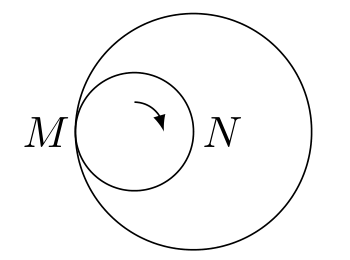
\includegraphics[width=4.8cm]{GaoKao/images/2011/jiangxi_science/q10_fig1.png}
\end{center}

        {\centering\begin{tabular*}{\linewidth}{@{}@{\extracolsep{\fill}}cccc@{}}
          \text{A. }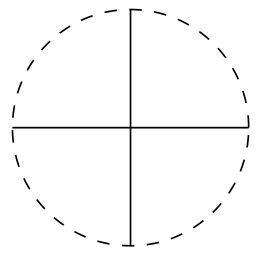
\includegraphics[width=0.15\paperwidth]{GaoKao/images/2011/jiangxi_science/q10_optA.png}  &  \text{B. }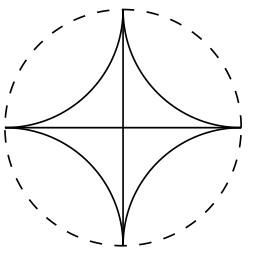
\includegraphics[width=0.15\paperwidth]{GaoKao/images/2011/jiangxi_science/q10_optB.png}  &  \text{C. }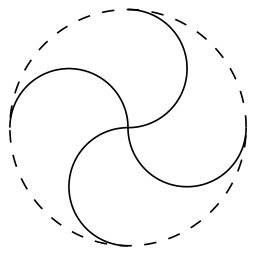
\includegraphics[width=0.15\paperwidth]{GaoKao/images/2011/jiangxi_science/q10_optC.png}  &  \text{D. }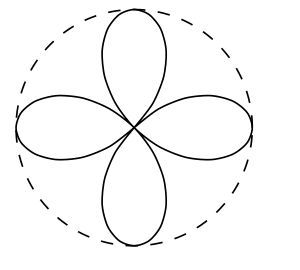
\includegraphics[width=0.15\paperwidth]{GaoKao/images/2011/jiangxi_science/q10_optD.png}
        \end{tabular*}\par}

    \end{enumerate}

\end{description}

\begin{description}

    \item[二、填空题]

    \begin{enumerate}[leftmargin=5pt]

      \addtocounter{enumi}{+10}

        \item 已知 \(|a| = |b| = 2\)，\((a + 2b) \cdot (a - b) = -2\)，则 \(a\) 与 \(b\) 的夹角为\rule[-0.3ex]{3em}{0.4pt}.

        \item 小波通过做游戏的方式来确定周末活动，他随机地往单位圆内投掷一点，若此点到圆心的距离大于 \(\frac{1}{2}\)，则周末去看电影；若此点到圆心的距离小于 \(\frac{1}{4}\)，则去打篮球；否则，在家看书. 则小波周末不在家看书的概率为\rule[-0.3ex]{3em}{0.4pt}.

        \item 下图是某算法程序框图，则程序运行后输出的结果是\rule[-0.3ex]{3em}{0.4pt}.

\begin{center}
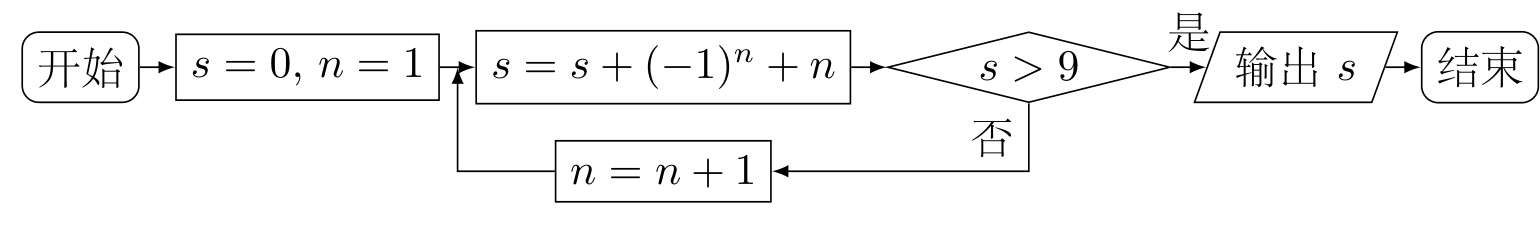
\includegraphics[width=0.96\linewidth]{GaoKao/images/2011/jiangxi_science/q13_fig1.png}
\end{center}

        \item 若椭圆 \(\frac{x^2}{a^2} + \frac{y^2}{b^2} = 1\) 的焦点在 \(x\) 轴上，过点 \(\left(1, \frac{1}{2}\right)\) 作圆 \(x^2 + y^2 = 1\) 的切线. 切点分别为 \(A\)，\(B\)，直线 \(AB\) 恰好经过椭圆的右焦点和上顶点，则椭圆方程是\rule[-0.3ex]{3em}{0.4pt}.

    \end{enumerate}

\end{description}

\begin{description}

    \item[三、选做题]

    \begin{enumerate}[leftmargin=5pt]

      \addtocounter{enumi}{+14}

        \item \textbf{【选修4-4：坐标系与参数方程】}

[A]
若曲线的极坐标方程为 \(\rho = 2 \sin \theta + 4 \cos \theta\)，以极点为原点，极轴为 \(x\) 轴正半轴建立直角坐标系，则该曲线的直角坐标方程为\rule[-0.3ex]{3em}{0.4pt}.

        \item [B]
对于实数 \(x\)，\(y\)，若 \(|x - 1| \leqslant 1\)，\(|y - 2| \leqslant 1\)，则 \(|x - 2y + 1|\) 的最大值为\rule[-0.3ex]{3em}{0.4pt}.

    \end{enumerate}

\end{description}

\begin{description}

    \item[四、解答题]

    \begin{enumerate}[leftmargin=5pt]

      \addtocounter{enumi}{+16}

        \item 某饮料公司招聘一名员工，现对其进行一项测试，以便确定工资级别. 公司准备了两种不同的饮料共 \(8\text{ 杯}\)，其颜色完全相同，并且其中 \(4\text{ 杯}\) 为 A 饮料，另外 \(4\text{ 杯}\) 为 B 饮料，公司要求此员工一一品尝后，从 \(8\text{ 杯}\) 饮料中选出 \(4\text{ 杯}\) A 饮料. 若 \(4\text{ 杯}\) 都选对，则月工资定为 \(3500\text{ 元}\)；若 \(4\text{ 杯}\) 选对 \(3\text{ 杯}\)，则月工资定为 \(2800\text{ 元}\)；否则月工资定为 \(2100\text{ 元}\). 令 \(X\) 表示此人选对 A 饮料的杯数. 假设此人对 A 和 B 两种饮料没有鉴别能力.

\begin{enumerate}
\item 求 \(X\) 的分布列；
\item 求此员工月工资的期望.
\end{enumerate}

        \item 在 \(\triangle ABC\) 中，角 \(A\)，\(B\)，\(C\) 的对边分别是 \(a\)，\(b\)，\(c\)，已知 \(\sin C + \cos C = 1 - \sin \frac{C}{2}\).
\begin{enumerate}
\item 求 \(\sin C\) 的值；
\item 若 \(a^2 + b^2 = 4(a + b) - 8\)，求边 \(c\) 的值.
\end{enumerate}

        \item 已知两个等比数列 \(\{a_{n}\}\)，\(\{b_{n}\}\)，满足 \(a_{1} = a\)（\(a > 0\)），\(b_{1} - a_{1} = 1\)，\(b_{2} - a_{2} = 2\)，\(b_{3} - a_{3} = 3\).
\begin{enumerate}
\item 若 \(a = 1\)，求数列 \(\{a_{n}\}\) 的通项公式；
\item 若数列 \(\{a_{n}\}\) 唯一，求 \(a\) 的值.
\end{enumerate}

        \item 设 \( f(x) = -\frac{1}{3} x^3 + \frac{1}{2} x^2 + 2ax \).
\begin{enumerate}
\item 若 \( f(x) \) 在 \( \left(\frac{2}{3}, +\infty\right) \) 上存在单调递增区间，求 \(a\) 的取值范围；
\item 当 \(0 < a < 2\) 时，\( f(x) \) 在 \([1, 4]\) 上的最小值为 \(-\frac{16}{3}\)，求 \( f(x) \) 在该区间上的最大值.
\end{enumerate}

        \item \(P(x_0, y_0)\)（\(x_0 \neq \pm a\)）是双曲线 \(E: \frac{x^2}{a^2} - \frac{y^2}{b^2} = 1\)（\(a > 0\)，\(b > 0\)）上一点，\(M\)，\(N\) 分别是双曲线 \(E\) 的左，右顶点. 直线 \(PM\)，\(PN\) 的斜率之积为 \(\frac{1}{5}\).
\begin{enumerate}
\item 求双曲线的离心率；
\item 过双曲线 \(E\) 的右焦点且斜率为 1 的直线交双曲线于 \(A\)，\(B\) 两点，\(O\) 为坐标原点，\(C\) 为双曲线上的一点. 满足 \(\overrightarrow{OC} = \lambda \overrightarrow{OA} + \overrightarrow{OB}\)，求 \(\lambda\) 的值.
\end{enumerate}

        \item \begin{enumerate}
    \item 如图，对于任一给定的四面体 \(A_{1}A_{2}A_{3}A_{4}\)，找出依次排列的四个相互平行的平面 \(\alpha_{1}\)，\(\alpha_{2}\)，\(\alpha_{3}\)，\(\alpha_{4}\)，使得 \(A_{i} \in \alpha_{i}\) （\(i = 1\)，\(2\)，\(3\)，\(4\)），且其中每相邻两个平面间的距离都相等；
    \item 给定依次排列的四个相互平行的平面 \(\alpha_{1}\)，\(\alpha_{2}\)，\(\alpha_{3}\)，\(\alpha_{4}\)，其中每相邻两个平面间的距离都为 1，若一个正四面体 \(A_{1}A_{2}A_{3}A_{4}\) 的四个顶点满足： \(A_{i} \in \alpha_{i}\) （\(i = 1\)，\(2\)，\(3\)，\(4\)），求该正四面体 \(A_{1}A_{2}A_{3}A_{4}\) 的体积.
\end{enumerate}

\begin{center}
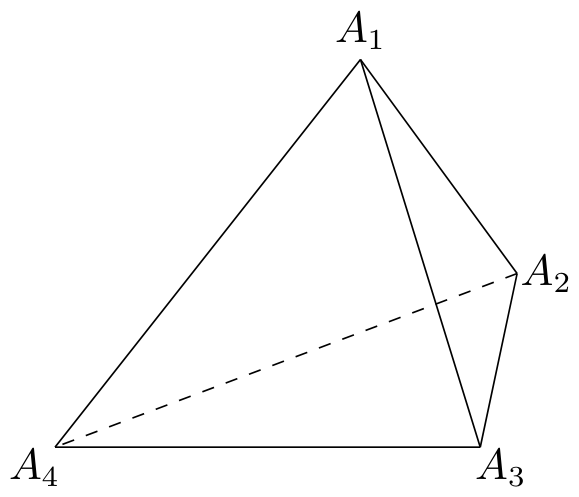
\includegraphics[width=5.6cm]{GaoKao/images/2011/jiangxi_science/q21_fig1.png}
\end{center}

    \end{enumerate}

\end{description}


\subsection{2011年江西卷（文）}\label{gk:2011年江西卷（文）}

\begin{description}

    \item[一、选择题]

    \begin{enumerate}[leftmargin=5pt]

        \item 若 \((x - \i)\i = y + 2\i\)，\(x\)，\(y \in \mathbb{R}\)，则复数 \(x + y\i =\)（\quad）

        {\centering\begin{tabular*}{\linewidth}{@{}@{\extracolsep{\fill}}llll@{}}
          \text{A. }\(-2 + \i\)  &  \text{B. }\(2 + \i\)  &  \text{C. }\(1 - 2\i\)  &  \text{D. }\(1 + 2\i\)
        \end{tabular*}\par}

        \item 若全集 \(U = \{1, 2, 3, 4, 5, 6\}\)，\(M = \{2, 3\}\)，\(N = \{1, 4\}\)，则集合 \(\{5, 6\}\) 等于（\quad）

        {\centering\begin{tabular*}{\linewidth}{@{}@{\extracolsep{\fill}}llll@{}}
          \text{A. }\(M \cup N\)  &  \text{B. }\(M \cap N\)  &  \text{C. }\((\complement_U M) \cup (\complement_U N)\)  &  \text{D. }\((\complement_U M) \cap (\complement_U N)\)
        \end{tabular*}\par}

        \item 若 \( f(x) = \frac{1}{\log_{\frac{1}{2}}(2x + 1)} \)，则 \( f(x) \) 的定义域为（\quad）

        {\centering\begin{tabular*}{\linewidth}{@{}@{\extracolsep{\fill}}llll@{}}
          \text{A. }\(\left(-\frac{1}{2}, 0\right)\)  &  \text{B. }\(\left(-\frac{1}{2}, +\infty\right)\)  &  \text{C. }\(\left(-\frac{1}{2}, 0\right) \cup (0, +\infty)\)  &  \text{D. }\(\left(-\frac{1}{2}, 2\right)\)
        \end{tabular*}\par}

        \item 曲线 \( y = {\mathrm{e}}^{x} \) 在点 \( A(0,1) \) 处的切线斜率为（\quad）

        {\centering\begin{tabular*}{\linewidth}{@{}@{\extracolsep{\fill}}llll@{}}
          \text{A. }\(1\)  &  \text{B. }\(2\)  &  \text{C. }\({\mathrm{e}}\)  &  \text{D. }\(\frac{1}{{\mathrm{e}}}\)
        \end{tabular*}\par}

        \item 设 \(\{a_{n}\}\) 为等差数列，公差 \(d = -2\)，\(S_{n}\) 为其前 \(n\) 项和. 若 \(S_{10} = S_{11}\)，则 \(a_{1} =\)（\quad）

        {\centering\begin{tabular*}{\linewidth}{@{}@{\extracolsep{\fill}}llll@{}}
          \text{A. }\(18\)  &  \text{B. }\(20\)  &  \text{C. }\(22\)  &  \text{D. }\(24\)
        \end{tabular*}\par}

        \item 观察下列各式： \(7^{2} = 49\)，\(7^{3} = 343\)，\(7^{4} = 2401\)，\(\cdots\)，则 \(7^{2011}\) 的末两位数字为（\quad）

        {\centering\begin{tabular*}{\linewidth}{@{}@{\extracolsep{\fill}}llll@{}}
          \text{A. }\(01\)  &  \text{B. }\(43\)  &  \text{C. }\(07\)  &  \text{D. }\(49\)
        \end{tabular*}\par}

        \item 为了普及环保知识，增强环保意识，某大学随机抽取 30 名学生参加环保知识测试，得分 （十分制） 如图所示，假设得分值的中位数为 \(m_{e}\)，众数为 \(m_{o}\)，平均值为 \(\overline{x}\)，则（\quad）

\begin{center}
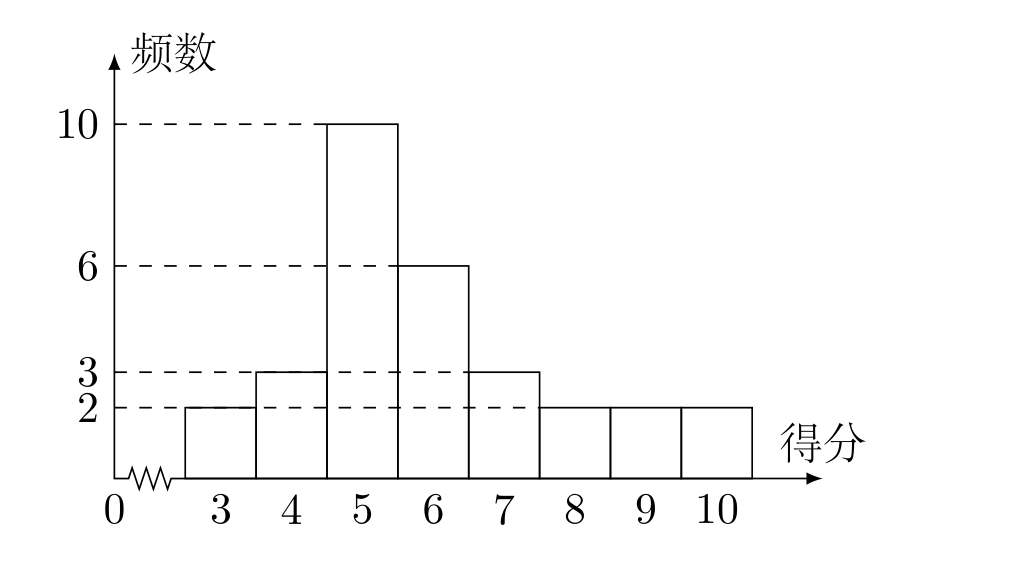
\includegraphics[width=0.72\linewidth]{GaoKao/images/2011/jiangxi_liberal/q7_fig1.png}
\end{center}

        {\centering\begin{tabular*}{\linewidth}{@{}@{\extracolsep{\fill}}llll@{}}
          \text{A. }\(m_{e} = m_{o} = \overline{x}\)  &  \text{B. }\(m_{e} = m_{o} < \overline{x}\)  &  \text{C. }\(m_{e} < m_{o} < \overline{x}\)  &  \text{D. }\(m_{o} < m_{e} < \overline{x}\)
        \end{tabular*}\par}

        \item 为了解儿子身高与其父亲身高的关系，随机抽取 5 对父子的身高数据如下：
\begin{center}
\renewcommand{\arraystretch}{1.1}
\begin{tabular}{c|ccccc}
父亲身高 \(x(\mathrm{cm})\) & 174 & 176 & 176 & 176 & 178 \\
\hline
儿子身高 \(y(\mathrm{cm})\) & 175 & 175 & 176 & 177 & 177
\end{tabular}
\end{center}
则 \(y\) 对 \(x\) 的线性回归方程为（\quad）

        {\centering\begin{tabular*}{\linewidth}{@{}@{\extracolsep{\fill}}llll@{}}
          \text{A. }\(y = x - 1\)  &  \text{B. }\(y = x + 1\)  &  \text{C. }\(y = 88 + \frac{1}{2} x\)  &  \text{D. }\(y = 176\)
        \end{tabular*}\par}

        \item 将长方体截去一个四棱锥，得到的几何体如图所示，则该几何体的左视图为（\quad）

\begin{center}
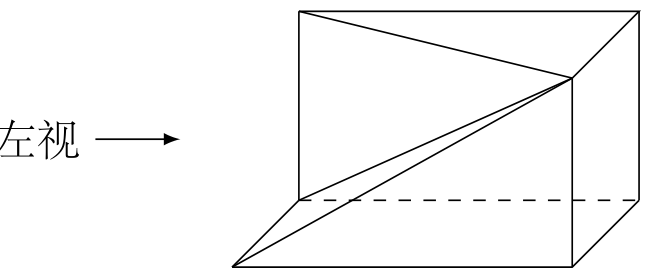
\includegraphics[width=5.9cm]{GaoKao/images/2011/jiangxi_liberal/q9_fig1.png}
\end{center}

        {\centering\begin{tabular*}{\linewidth}{@{}@{\extracolsep{\fill}}cccc@{}}
          \text{A. }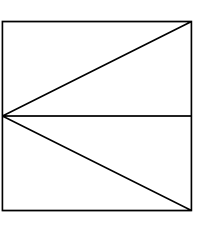
\includegraphics[width=0.15\paperwidth]{GaoKao/images/2011/jiangxi_liberal/q9_choiceA.png}  &  \text{B. }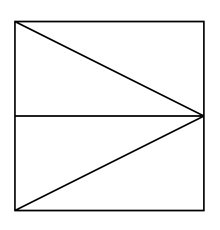
\includegraphics[width=0.15\paperwidth]{GaoKao/images/2011/jiangxi_liberal/q9_choiceB.png}  &  \text{C. }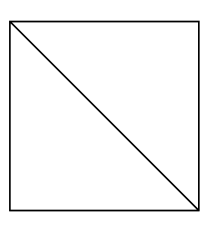
\includegraphics[width=0.15\paperwidth]{GaoKao/images/2011/jiangxi_liberal/q9_choiceC.png}  &  \text{D. }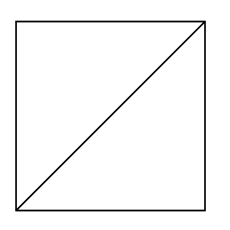
\includegraphics[width=0.15\paperwidth]{GaoKao/images/2011/jiangxi_liberal/q9_choiceD.png}
        \end{tabular*}\par}

        \item 如图，一个“凸轮”放置于直角坐标系 \(x\) 轴上方，其“底端”落在原点 \(O\) 处，一顶点及中心 \(M\) 在 \(y\) 轴正半轴上，它的外围由以正三角形的顶点为圆心，以正三角形的边长为半径的三段等弧组成. 今使“凸轮”沿 \(x\) 轴正向滚动前进，在滚动过程中“凸轮”每时每刻都有一个“最高点”，其中心也在不断移动位置. 则在“凸轮”滚动一周的过程中，将其“最高点”和“中心点”所形成的图形按上，下放置，应大致为（\quad）

\begin{center}
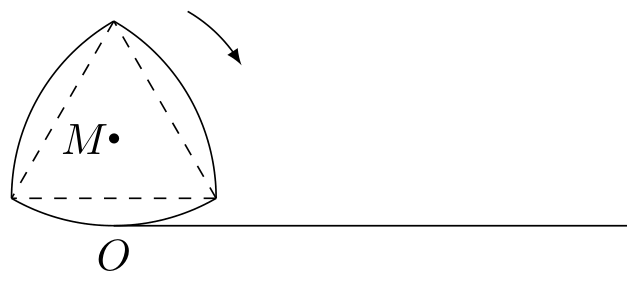
\includegraphics[width=5.5cm]{GaoKao/images/2011/jiangxi_liberal/q10_fig1.png}
\end{center}

        {\centering\begin{tabular*}{\linewidth}{@{}@{\extracolsep{\fill}}cccc@{}}
          \text{A. }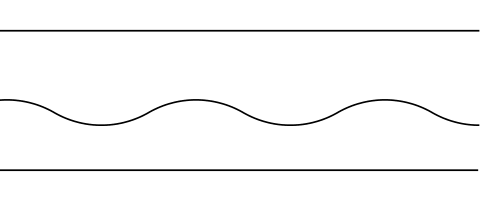
\includegraphics[width=0.15\paperwidth]{GaoKao/images/2011/jiangxi_liberal/q10_choiceA.png}  &  \text{B. }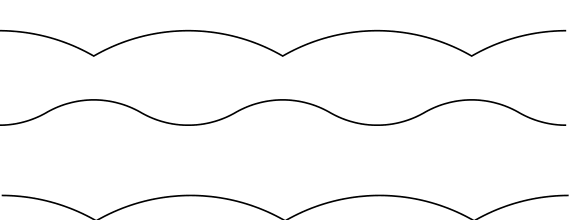
\includegraphics[width=0.15\paperwidth]{GaoKao/images/2011/jiangxi_liberal/q10_choiceB.png}  &  \text{C. }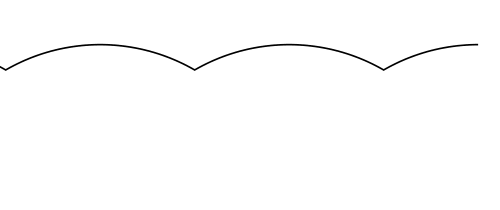
\includegraphics[width=0.15\paperwidth]{GaoKao/images/2011/jiangxi_liberal/q10_choiceC.png}  &  \text{D. }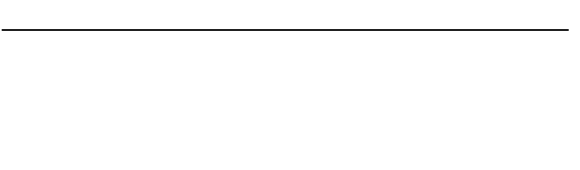
\includegraphics[width=0.15\paperwidth]{GaoKao/images/2011/jiangxi_liberal/q10_choiceD.png}
        \end{tabular*}\par}

    \end{enumerate}

\end{description}

\begin{description}

    \item[二、填空题]

    \begin{enumerate}[leftmargin=5pt]

      \addtocounter{enumi}{+10}

        \item 已知两个单位向量 \(e_{1}\)，\(e_{2}\) 的夹角为 \( \frac{\pi}{3} \)，若向量 \(b_{1} = e_{1} - 2e_{2}\)，\(b_{2} = 3e_{1} + 4e_{2}\)，则 \( b_{1} \cdot b_{2} = \)\rule[-0.3ex]{3em}{0.4pt}.

        \item 若双曲线 \(\frac{y^2}{16} - \frac{x^2}{m} = 1\) 的离心率 \(e = 2\)，则 \(m = \)\rule[-0.3ex]{3em}{0.4pt}.

        \item 下图是某算法程序框图，则程序运行后输出的结果是\rule[-0.3ex]{3em}{0.4pt}.

\begin{center}
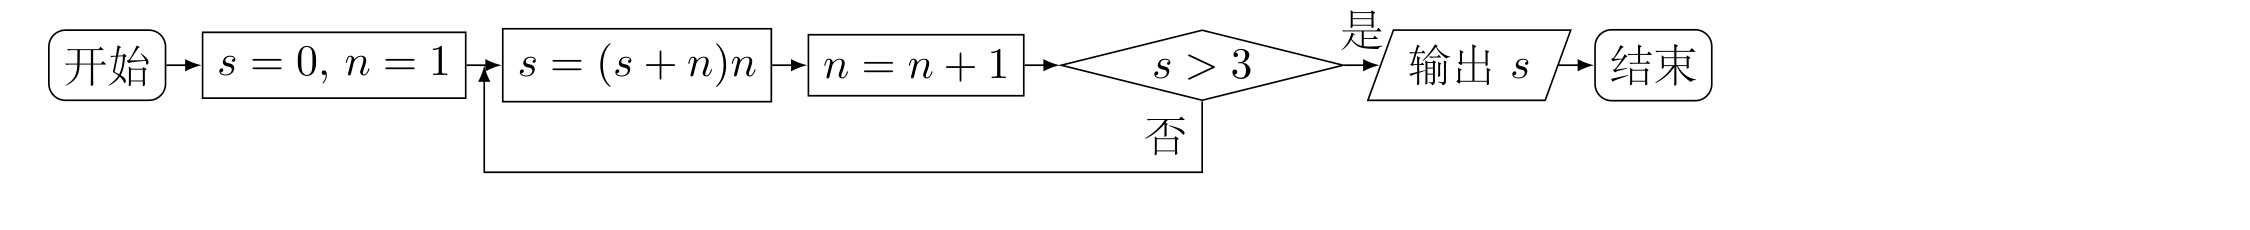
\includegraphics[width=0.96\linewidth]{GaoKao/images/2011/jiangxi_liberal/q13_fig1.png}
\end{center}

        \item 已知角 \(\theta\) 的顶点为坐标原点，始边为 \(x\) 轴的正半轴. 若 \(P(4, y)\) 是角 \(\theta\) 终边上一点，且 \(\sin \theta = -\frac{2\sqrt{5}}{5}\)，则 \(y =\rule[-0.3ex]{3em}{0.4pt}\).

        \item 对于 \(x \in \mathbb{R}\)，不等式 \(|x + 10| - |x - 2| \geqslant 8\) 的解集为\rule[-0.3ex]{3em}{0.4pt}.

    \end{enumerate}

\end{description}

\begin{description}

    \item[三、解答题]

    \begin{enumerate}[leftmargin=5pt]

      \addtocounter{enumi}{+15}

        \item 某饮料公司对一名员工进行测试以便确定其考评级别. 公司准备了两种不同的饮料共5杯，其颜色完全相同，并且其中3杯为A饮料，另外2杯为B饮料，公司要求此员工一一品尝后，从5杯饮料中选出3杯A饮料. 若 该员工3杯都选对，则评为优秀；若3杯选对2杯，则评为良好；否则评为及格. 假设此人对 \(A\) 和 \(B\) 两种饮料没有鉴别能力.
\begin{enumerate}
\item 求此人被评为优秀的概率；
\item 求此人被评为良好及以上的概率.
\end{enumerate}

        \item 在 \(\triangle ABC\) 中，\(A\)，\(B\)，\(C\) 的对边分别是 \(a\)，\(b\)，\(c\). 已知 \(3a \cos A = c \cos B + b \cos C\).
\begin{enumerate}
\item 求 \( \cos A \) 的值；
\item 若 \(a = 1\)，\(\cos B + \cos C = \frac{2\sqrt{3}}{3}\)，求边 \(c\) 的值.
\end{enumerate}

        \item 如图，在 \(\triangle ABC\) 中，\(\angle B = \frac{\pi}{2}\)，\(AB = BC = 2\). \(P\) 为 \(AB\) 边上动一点，\(PD \parallel BC\) 交 \(AC\) 于点 \(D\)，现将 \(\triangle PDA\) 沿 \(PD\) 翻折至 \(\triangle PDA'\)，使平面 \(PDA' \perp\) 平面 \(PBCD\).
\begin{enumerate}
\item 当棱锥 \(A' - PBCD\) 的体积最大时，求 \(PA\) 的长；
\item 若点 \(P\) 为 \(AB\) 的中点，\(E\) 为 \(A'C\) 的中点，求证： \(A'B \perp DE\).
\end{enumerate}

\begin{center}
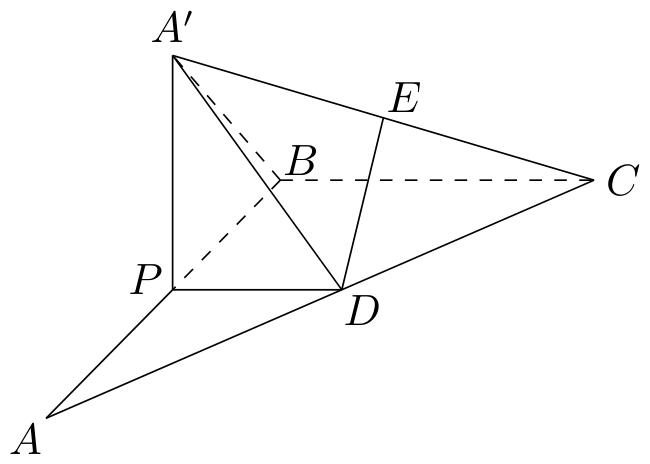
\includegraphics[width=6.4cm]{GaoKao/images/2011/jiangxi_liberal/q18_fig1.png}
\end{center}

        \item 已知过抛物线 \( y^{2} = 2px \) （\( p > 0 \)） 的焦点，斜率为 \( 2\sqrt{2} \) 的直线交抛物线于 \( A(x_{1}, y_{1}) \)，\( B(x_{2}, y_{2}) \) （\( x_{1} < x_{2} \)） 两点，且 \( |AB| = 9 \).
\begin{enumerate}
\item 求该抛物线的方程；
\item O 为坐标原点，C 为抛物线上一点. 若 \( \overrightarrow{OC} = \overrightarrow{OA} + \lambda \overrightarrow{OB} \)，求 \( \lambda \) 的值.
\end{enumerate}

        \item 设 \( f(x) = \frac{1}{3} x^3 + mx^2 + nx \).
\begin{enumerate}
\item 如果 \( g(x) = f'(x) - 2x - 3 \) 在 \( x = -2 \) 处取得最小值 \(-5\)，求 \( f(x) \) 的解析式；
\item 如果 \(m + n < 10\) （\(m\)，\(n \in \mathbf{N}_+\)），\(f(x)\) 的单调递减区间的长度是正整数，试求 \(m\) 和 \(n\) 的值. （注：区间 \((a, b)\) 的长度为 \(b - a\)）
\end{enumerate}

        \item \begin{enumerate}
\item 已知两个等比数列 \(\{a_{n}\}\)，\(\{b_{n}\}\)，满足 \(a_{1} = a\)（\(a > 0\)），\(b_{1} - a_{1} = 1\)，\(b_{2} - a_{2} = 2\)，\(b_{3} - a_{3} = 3\)，若数列 \(\{a_{n}\}\) 唯一，求 \(a\) 的值；
\item 是否存在两个等比数列 \(\{a_{n}\}\)，\(\{b_{n}\}\)，使得 \(b_{1} - a_{1}\)，\(b_{2} - a_{2}\)，\(b_{3} - a_{3}\)，\(b_{4} - a_{4}\) 成公差不为 0 的等差数列？ 若存在，求 \(\{a_{n}\}\)，\(\{b_{n}\}\) 的通项公式；若不存在，说明理由.
\end{enumerate}

    \end{enumerate}

\end{description}


\subsection{2011年辽宁卷（理）}\label{gk:2011年辽宁卷（理）}

\begin{description}

    \item[一、选择题]

    \begin{enumerate}[leftmargin=5pt]

        \item 若 \(a\) 为正实数，\(\i\) 为虚数单位，\(\left|\frac{a + \i}{\i}\right| = 2\)，则 \(a =\)（\quad）

        {\centering\begin{tabular*}{\linewidth}{@{}@{\extracolsep{\fill}}llll@{}}
          \text{A. }2  &  \text{B. }\(\sqrt{3}\)  &  \text{C. }\(\sqrt{2}\)  &  \text{D. }1
        \end{tabular*}\par}

        \item 已知 \(M\)，\(N\) 为集合 \(I\) 的非空真子集，且 \(M\)，\(N\) 不相等，若 \(N \cap \complement_I M = \varnothing\)，则 \(M \cup N =\)（\quad）

        {\centering\begin{tabular*}{\linewidth}{@{}@{\extracolsep{\fill}}llll@{}}
          \text{A. }M  &  \text{B. }N  &  \text{C. }I  &  \text{D. }\(\varnothing\)
        \end{tabular*}\par}

        \item 已知 \(F\) 是抛物线 \(y^{2} = x\) 的焦点，\(A\)，\(B\) 是该抛物线上的两点，\(|AF| + |BF| = 3\)，则线段 \(AB\) 的中点到 \(y\) 轴的距离为（\quad）

        {\centering\begin{tabular*}{\linewidth}{@{}@{\extracolsep{\fill}}llll@{}}
          \text{A. }\( \frac{3}{4} \)  &  \text{B. }1  &  \text{C. }\( \frac{5}{4} \)  &  \text{D. }\( \frac{7}{4} \)
        \end{tabular*}\par}

        \item \(\triangle ABC\) 的三个内角 \(A\)，\(B\)，\(C\) 所对的边分别为 \(a\)，\(b\)，\(c\)，并且有 \(a \sin A \sin B + b \cos^2 A = \sqrt{2} a\)，则 \(\frac{b}{a} =\)（\quad）

        {\centering\begin{tabular*}{\linewidth}{@{}@{\extracolsep{\fill}}llll@{}}
          \text{A. }\(2 \sqrt{3}\)  &  \text{B. }\(2 \sqrt{2}\)  &  \text{C. }\(\sqrt{3}\)  &  \text{D. }\(\sqrt{2}\)
        \end{tabular*}\par}

        \item 从 1， 2， 3， 4， 5 中任取 2 个不同的数，事件 \(A =\) “取到的 2 个数之和为偶数”，事件 \(B =\) “取到的 2 个数均为偶数”，则 \( P(B \mid A) = \)（\quad）

        {\centering\begin{tabular*}{\linewidth}{@{}@{\extracolsep{\fill}}llll@{}}
          \text{A. }\(\frac{1}{8}\)  &  \text{B. }\(\frac{1}{4}\)  &  \text{C. }\(\frac{2}{5}\)  &  \text{D. }\(\frac{1}{2}\)
        \end{tabular*}\par}

        \item 执行下面的程序框图，如果输入的 \(n\) 是 4，则输出的 \(p\) 是（\quad）

\begin{center}
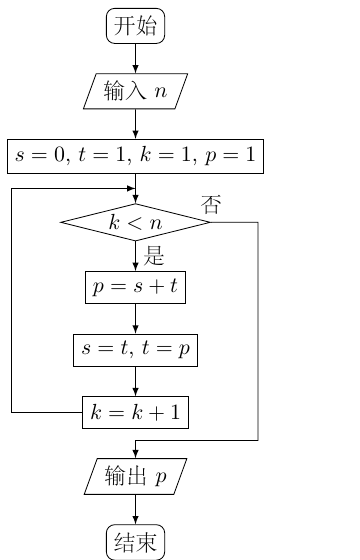
\includegraphics[width=0.42\linewidth]{GaoKao/images/2011/liaoning_science/q6_fig1.png}
\end{center}

        {\centering\begin{tabular*}{\linewidth}{@{}@{\extracolsep{\fill}}llll@{}}
          \text{A. }8  &  \text{B. }5  &  \text{C. }3  &  \text{D. }2
        \end{tabular*}\par}

        \item 设 \(\sin \left(\frac{\pi}{4} + \theta\right) = \frac{1}{3}\)，则 \(\sin 2\theta =\)（\quad）

        {\centering\begin{tabular*}{\linewidth}{@{}@{\extracolsep{\fill}}llll@{}}
          \text{A. }\(-\frac{7}{9}\)  &  \text{B. }\(-\frac{1}{9}\)  &  \text{C. }\( \frac{1}{9} \)  &  \text{D. }\( \frac{7}{9} \)
        \end{tabular*}\par}

        \item 如图，四棱锥 \(S - ABCD\) 的底面为正方形，\(SD \perp\) 底面 \(ABCD\)，则下列结论中不正确的是（\quad）

\begin{center}
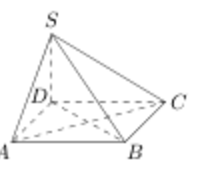
\includegraphics[width=4.1cm]{GaoKao/images/2011/liaoning_science/q8_fig1.png}
\end{center}

        {\centering\begin{tabular*}{\linewidth}{@{}@{\extracolsep{\fill}}llll@{}}
          \text{A. }\(AC \perp SB\)  &  \text{B. }\(AB \parallel\) 平面 \(SCD\)  &  \text{C. }\(SA\) 与平面 \(SBD\) 所成的角等于 \(SC\) 与平面 \(SBD\) 所成的角  &  \text{D. }\(AB\) 与 \(SC\) 所成的角等于 \(DC\) 与 \(SA\) 所成的角
        \end{tabular*}\par}

        \item 设函数 \( f(x) = \begin{cases}
2^{1 - x}, & x \leqslant 1,\\
1 - \log_2 x, & x > 1,
\end{cases} \) 则满足 \( f(x) \leqslant 2 \) 的 \( x \) 取值范围是（\quad）

        {\centering\begin{tabular*}{\linewidth}{@{}@{\extracolsep{\fill}}llll@{}}
          \text{A. }\([-1, 2]\)  &  \text{B. }\([0,2]\)  &  \text{C. }\([1, +\infty)\)  &  \text{D. }\([0, +\infty)\)
        \end{tabular*}\par}

        \item 若 \(a\)，\(b\)，\(c\) 均为单位向量，且 \(a \cdot b = 0\)，\((a - c) \cdot (b - c) \leqslant 0\)，则 \(\lvert a + b - c \rvert\) 的最大值为（\quad）

        {\centering\begin{tabular*}{\linewidth}{@{}@{\extracolsep{\fill}}llll@{}}
          \text{A. }\(\sqrt{2} - 1\)  &  \text{B. }1  &  \text{C. }\(\sqrt{2}\)  &  \text{D. }2
        \end{tabular*}\par}

        \item 函数 \( f(x) \) 的定义域为 \( \mathbb{R} \)，\( f(-1) = 2 \)，对任意 \( x \in \mathbb{R} \)，\( f'(x) > 2 \)，则 \( f(x) > 2x + 4 \) 的解集为（\quad）

        {\centering\begin{tabular*}{\linewidth}{@{}@{\extracolsep{\fill}}llll@{}}
          \text{A. }\((-1, 1)\)  &  \text{B. }\((-1, +\infty)\)  &  \text{C. }\((- \infty, -1)\)  &  \text{D. }\((-\infty, +\infty)\)
        \end{tabular*}\par}

        \item 已知球的直径 \(SC = 4\)，\(A\)，\(B\) 是该球球面上的两点，\(AB = \sqrt{3}\)，\(\angle ASC = \angle BSC = 30^\circ\)，则棱锥 \(S - ABC\) 的体积为（\quad）

        {\centering\begin{tabular*}{\linewidth}{@{}@{\extracolsep{\fill}}llll@{}}
          \text{A. }\(3\sqrt{3}\)  &  \text{B. }\(2\sqrt{3}\)  &  \text{C. }\(\sqrt{3}\)  &  \text{D. }1
        \end{tabular*}\par}

    \end{enumerate}

\end{description}

\begin{description}

    \item[二、填空题]

    \begin{enumerate}[leftmargin=5pt]

      \addtocounter{enumi}{+12}

        \item 已知点 \((2,3)\) 在双曲线 \(C: \frac{x^2}{a^2} - \frac{y^2}{b^2} = 1 \) （\(a > 0, b > 0\)）上，\(C\) 的焦距为 4，则它的离心率为\rule[-0.3ex]{3em}{0.4pt}.

        \item 调查了某地若干户家庭的年收入 \(x\) （单位：万元） 和年饮食支出 \(y\) （单位：万元），调查显示年收入 \(x\) 与年饮食支出 \(y\) 具有线性相关关系. 并由调查数据得到 \(y\) 对 \(x\) 的回归直线方程： \(\hat{y} = 0.254x + 0.321\). 由回归直线方程可知，家庭收入每增加 1 万元，年饮食支出平均增加\rule[-0.3ex]{3em}{0.4pt} 万元.

        \item 一个正三棱柱的侧棱长和底面边长相等，体积为 \(2 \sqrt{3}\)，它的三视图中的俯视图如图所示，左视图是一个矩形，则这个矩形的面积是\rule[-0.3ex]{3em}{0.4pt}

\begin{center}
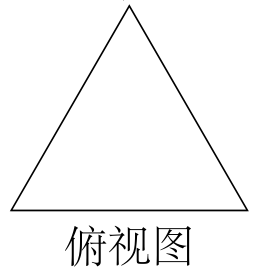
\includegraphics[width=2.5cm]{GaoKao/images/2011/liaoning_science/q15_fig1.png}
\end{center}

        \item 已知函数 \( f(x) = A \tan (\omega x + \varphi) \)（\( \omega > 0, |\varphi| < \frac{\pi}{2} \)），\( y = f(x) \) 的部分图象如图，则 \( f\left(\frac{\pi}{24}\right) = \)\rule[-0.3ex]{3em}{0.4pt}.

\begin{center}
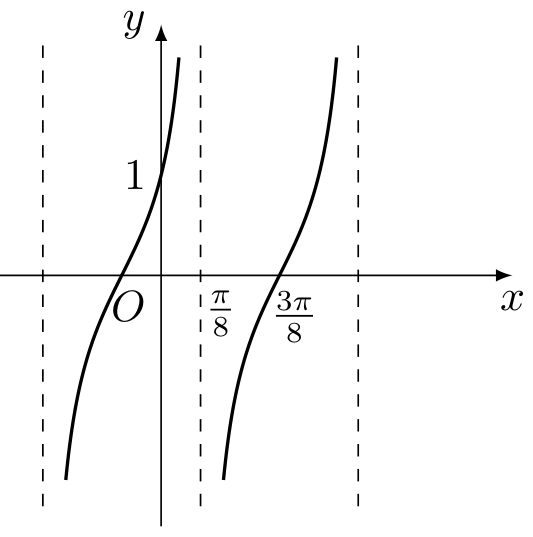
\includegraphics[width=7.6cm]{GaoKao/images/2011/liaoning_science/q16_fig1.png}
\end{center}

    \end{enumerate}

\end{description}

\begin{description}

    \item[三、解答题]

    \begin{enumerate}[leftmargin=5pt]

      \addtocounter{enumi}{+16}

        \item 已知等差数列 \(\{a_{n}\}\) 满足 \(a_{2} = 0\)，\(a_{6} + a_{8} = -10\).
\begin{enumerate}
\item 求数列 \( \{a_{n}\} \) 的通项公式；
\item 求数列 \( \left\{\frac{a_{n}}{2^{n-1}}\right\} \) 的前 \(n\) 项和.
\end{enumerate}

        \item 如图，四边形 \(ABCD\) 为正方形，\(PD \perp\) 平面 \(ABCD\)，\(PD \parallel QA\)，\(QA = AB = \frac{1}{2} PD\).
\begin{enumerate}
\item 证明：平面 \(PQC \perp\) 平面 \(DCQ\)；
\item 求二面角 \(Q - BP - C\) 的余弦值.
\end{enumerate}

\begin{center}
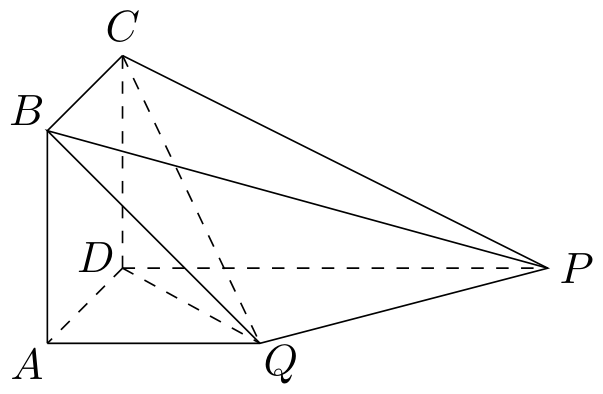
\includegraphics[width=7.2cm]{GaoKao/images/2011/liaoning_science/q18_fig1.png}
\end{center}

        \item 某农场计划种植某种新作物，为此对这种作物的两个品种（分别称为品种甲和品种乙）进行田间试验，选取两大块地. 每大块地分成 \(n\) 小块地. 在总共 \(2n\) 小块地中，随机选 \(n\) 小块地种植品种甲，另外 \(n\) 小块地种植品种乙.
\begin{enumerate}
\item 假设 \(n = 4\)，在第一大块地中，种植品种甲的小块地的数目记为 \(X\)，求 \(X\) 的分布列和数学期望.
\item 试验时每大块地分成 \(8\) 小块，即 \(n = 8\)，试验结束后得到品种甲和品种乙在各小块地上的每公顷产量 （单位： \(\mathrm{kg/hm^2}\)）如下表：
\begin{center}
\begin{tabular}{c|cccccccc}
\hline
品种甲 & 403 & 397 & 390 & 404 & 388 & 400 & 412 & 406 \\
\hline
品种乙 & 419 & 403 & 412 & 418 & 408 & 423 & 400 & 413 \\
\hline
\end{tabular}
\end{center}
分别求品种甲和品种乙每公顷产量的样本平均数和样本方差；根据试验结果，你应该种植哪一品种？

附：样本数据 \(x_{1}\)，\(x_{2}\)，\(\cdots\)，\(x_{n}\) 的样本方差 \(s^{2} = \frac{1}{n}[(x_{1} - \overline{x})^{2} + (x_{2} - \overline{x})^{2} + \cdots + (x_{n} - \overline{x})^{2}]\)，其中 \(\overline{x}\) 为样本平均数.
\end{enumerate}

        \item 已知函数 \( f(x) = \ln x - ax^2 + (2 - a)x \).
\begin{enumerate}
\item 讨论 \(f(x)\) 的单调性；
\item 设 \(a > 0\)，证明：当 \(0 < x < \frac{1}{a}\) 时，\(f\left(\frac{1}{a} + x\right) > f\left(\frac{1}{a} - x\right)\)；
\item 若函数 \( y = f(x) \) 的图象与 \( x \) 轴交于 \(A\)，\(B\) 两点，线段 \(AB\) 中点的横坐标为 \( x_0 \)，证明：\( f'(x_0) < 0 \).
\end{enumerate}

        \item 如图，已知椭圆 \(C_1\) 的中心在原点 \(O\)，长轴左，右端点 \(M\)，\(N\) 在 \(x\) 轴上，椭圆 \(C_2\) 的短轴为 \(MN\)，且 \(C_1\)，\(C_2\) 的离心率都为 \(e\). 直线 \(l \perp MN\)，\(l\) 与 \(C_1\) 交于两点，与 \(C_2\) 交于两点，这四点按纵坐标从大到小依次为 \(A\)，\(B\)，\(C\)，\(D\).
\begin{enumerate}
\item 设 \(e = \frac{1}{2}\)，求 \(|BC|\) 与 \(|AD|\) 的比值.
\item 当 \(e\) 变化时，是否存在直线 \(l\)，使得 \(BO \parallel AN\)，并说明理由.
\end{enumerate}

\begin{center}
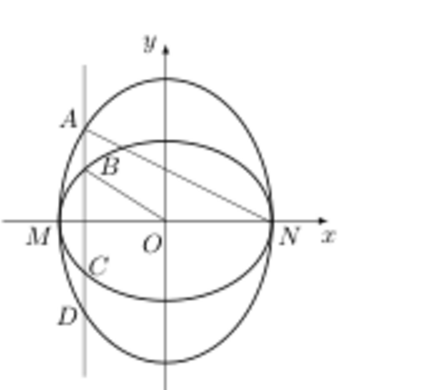
\includegraphics[width=6.0cm]{GaoKao/images/2011/liaoning_science/q20_fig1.png}
\end{center}

    \end{enumerate}

\end{description}

\begin{description}

    \item[四、选考题]

    \begin{enumerate}[leftmargin=5pt]

      \addtocounter{enumi}{+21}

        \item \textbf{【选修4-1：几何证明选讲】}

如图，\(A\)，\(B\)，\(C\)，\(D\) 四点在同一圆上，\(AD\) 的延长线与 \(BC\) 的延长线交于 \(E\) 点，且 \(EC = ED\).
\begin{enumerate}
\item 证明： \(CD \parallel AB\)；
\item 延长 \(CD\) 到 \(F\)，延长 \(DC\) 到 \(G\)，使得 \(EF = EG\)，证明： \(A\)，\(B\)，\(G\)，\(F\) 四点共圆.
\end{enumerate}

\begin{center}
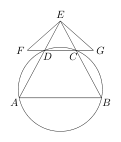
\includegraphics[width=5.6cm]{GaoKao/images/2011/liaoning_science/q22_fig1.png}
\end{center}

        \item \textbf{【选修4-4：坐标系与参数方程】}

在平面直角坐标系 \(xOy\) 中，曲线 \(C_1\) 的参数方程为 \(\begin{cases}
x = \cos \varphi,\\
y = \sin \varphi.
\end{cases}\) （\(\varphi\) 为参数）. 曲线 \(C_2\) 的参数方程为 \(\begin{cases}
x = a\cos \varphi,\\
y = b\sin \varphi,
\end{cases}\) （\(a > b > 0\)，\(\varphi\) 为参数）. 在以 \(O\) 为极点，\(x\) 轴的正半轴为极轴的极坐标系中，射线 \(l: \theta = \alpha\) 与 \(C_1\)，\(C_2\) 各有一个交点. 当 \(\alpha = 0\) 时，这两个交点间的距离为 2，当 \(\alpha = \frac{\pi}{2}\) 时，这两个交点重合.
\begin{enumerate}
\item 分别说明 \(C_1\)，\(C_2\) 是什么曲线，并求出 \(a\) 与 \(b\) 的值；
\item 设当 \(\alpha = \frac{\pi}{2}\) 时，\(l\) 与 \(C_1\)，\(C_2\) 的交点分别为 \(A_1\)，\(B_1\)，当 \(\alpha = -\frac{\pi}{4}\) 时，\(l\) 与 \(C_1\)，\(C_2\) 的交点分别为 \(A_2\)，\(B_2\)，求四边形 \(A_1A_2B_2B_1\) 的面积.
\end{enumerate}

        \item \textbf{【选修4-5：不等式选讲】}

已知函数 \(f(x) = |x - 2| - |x - 5|\).
\begin{enumerate}
\item 证明： \(-3 \leqslant f(x) \leqslant 3\).
\item 求不等式 \( f(x) \geqslant x^{2} - 8x + 15 \) 的解集.
\end{enumerate}

    \end{enumerate}

\end{description}


\subsection{2011年辽宁卷（文）}\label{gk:2011年辽宁卷（文）}

\begin{description}

    \item[一、选择题]

    \begin{enumerate}[leftmargin=5pt]

        \item 已知集合 \(A = \{x \mid x > 1\}\)，\(B = \{x \mid -1 < x < 2\}\)，则 \(A \cap B =\)（\quad）

        {\centering\begin{tabular*}{\linewidth}{@{}@{\extracolsep{\fill}}llll@{}}
          \text{A. }\(\{x\mid -1 < x < 2\}\)  &  \text{B. }\( \{x \mid x > -1\} \)  &  \text{C. }\( \{x \mid -1 < x < 1\} \)  &  \text{D. }\( \{x \mid 1 < x < 2\} \)
        \end{tabular*}\par}

        \item \(\i\) 为虚数单位，\(\frac{1}{\i} + \frac{1}{\i^{3}} + \frac{1}{\i^{5}} + \frac{1}{\i^{7}} =\)（\quad）

        {\centering\begin{tabular*}{\linewidth}{@{}@{\extracolsep{\fill}}llll@{}}
          \text{A. }\(0\)  &  \text{B. }\(2\i\)  &  \text{C. }\(-2\i\)  &  \text{D. }\(4\i\)
        \end{tabular*}\par}

        \item 已知向量 \(\bm{a} = (2,1)\)，\(\bm{b} = (-1,k)\)，\(\bm{a} \cdot (2\bm{a} - \bm{b}) = 0\)，则 \(k =\)（\quad）

        {\centering\begin{tabular*}{\linewidth}{@{}@{\extracolsep{\fill}}llll@{}}
          \text{A. }\(-12\)  &  \text{B. }\(-6\)  &  \text{C. }\(6\)  &  \text{D. }\(12\)
        \end{tabular*}\par}

        \item 已知命题 \(p: \exists n \in \mathbb{N}\)，\(2^n > 1000\)，则 \(\neg p\) 为（\quad）

        {\centering\begin{tabular*}{\linewidth}{@{}@{\extracolsep{\fill}}llll@{}}
          \text{A. }\(\forall n\in \mathbb{N},2^{n}\leqslant 1000\)  &  \text{B. }\(\forall n\in \mathbb{N}\)，\(2^n >1000\)  &  \text{C. }\(\exists n\in \mathbb{N}\)，\(2^n\leqslant 1000\)  &  \text{D. }\(\exists n\in \mathbb{N}\)，\(2^n < 1000\)
        \end{tabular*}\par}

        \item 若等比数列 \(\{a_{n}\}\) 满足 \(a_{n}a_{n + 1} = 16^{n}\)，则公比为（\quad）

        {\centering\begin{tabular*}{\linewidth}{@{}@{\extracolsep{\fill}}llll@{}}
          \text{A. }\(2\)  &  \text{B. }\(4\)  &  \text{C. }\(8\)  &  \text{D. }\(16\)
        \end{tabular*}\par}

        \item 若函数 \( f(x) = \frac{x}{(2x + 1)(x - a)} \) 为奇函数，则 \( a = \)（\quad）

        {\centering\begin{tabular*}{\linewidth}{@{}@{\extracolsep{\fill}}llll@{}}
          \text{A. }\(\frac{1}{2}\)  &  \text{B. }\( \frac{2}{3} \)  &  \text{C. }\(\frac{3}{4}\)  &  \text{D. }\(1\)
        \end{tabular*}\par}

        \item 已知 \(F\) 是抛物线 \(y^{2}=x\) 的焦点，\(A\)，\(B\) 是该抛物线上的两点，\(|AF|+|BF|=3\)，则线段 \(AB\) 的中点到 \(y\) 轴的距离为（\quad）

        {\centering\begin{tabular*}{\linewidth}{@{}@{\extracolsep{\fill}}llll@{}}
          \text{A. }\( \frac{3}{4} \)  &  \text{B. }\(1\)  &  \text{C. }\( \frac{5}{4} \)  &  \text{D. }\( \frac{7}{4} \)
        \end{tabular*}\par}

        \item 一个正三棱柱的侧棱长和底面边长相等，体积为 \(2\sqrt{3}\)，它的三视图中的俯视图如图所示，左视图是一个矩形，则这个矩形的面积是（\quad）

\begin{center}
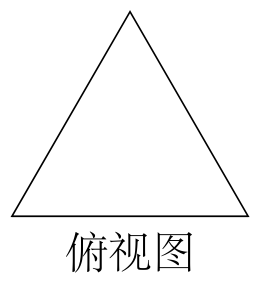
\includegraphics[width=2.5cm]{GaoKao/images/2011/liaoning_liberal/q8_fig1.png}
\end{center}

        {\centering\begin{tabular*}{\linewidth}{@{}@{\extracolsep{\fill}}llll@{}}
          \text{A. }\(4\)  &  \text{B. }\(2\sqrt{3}\)  &  \text{C. }\(2\)  &  \text{D. }\(\sqrt{3}\)
        \end{tabular*}\par}

        \item 执行下面的程序框图，如果输入的 \(n\) 是 4，则输出的 \(p\) 是（\quad）

\begin{center}
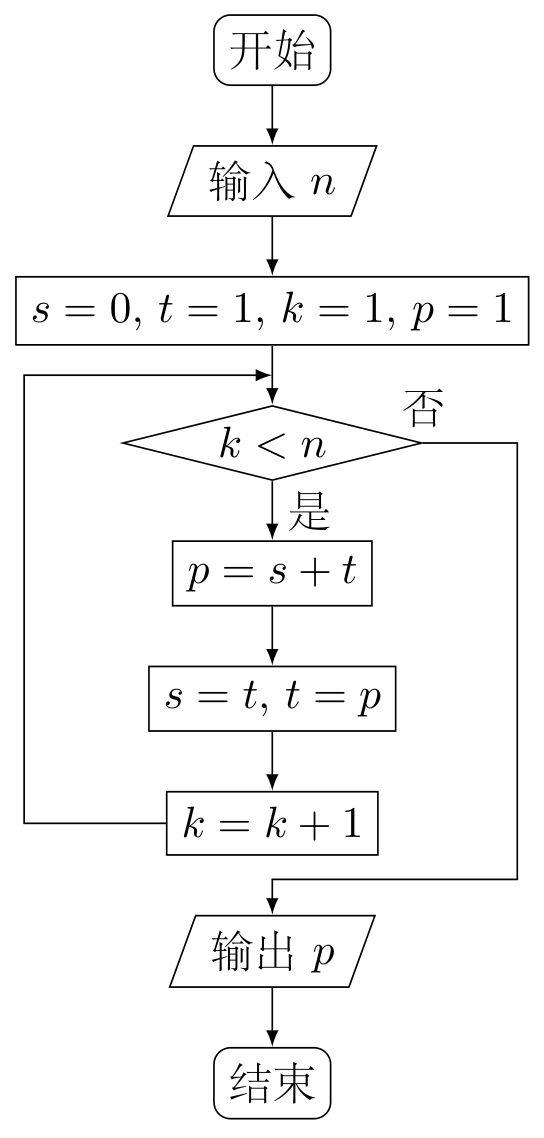
\includegraphics[width=0.52\linewidth]{GaoKao/images/2011/liaoning_liberal/q10_fig1.png}
\end{center}

        {\centering\begin{tabular*}{\linewidth}{@{}@{\extracolsep{\fill}}llll@{}}
          \text{A. }\(8\)  &  \text{B. }\(5\)  &  \text{C. }\(3\)  &  \text{D. }\(2\)
        \end{tabular*}\par}

        \item 已知球的直径 \(SC = 4\)，\(A\)，\(B\) 是该球球面上的两点，\(AB = 2\)，\(\angle ASC = \angle BSC = 45^\circ\)，则棱锥 \(S-ABC\) 的体积为（\quad）

        {\centering\begin{tabular*}{\linewidth}{@{}@{\extracolsep{\fill}}llll@{}}
          \text{A. }\(\frac{\sqrt{3}}{3}\)  &  \text{B. }\(\frac{2\sqrt{3}}{3}\)  &  \text{C. }\(\frac{4\sqrt{3}}{3}\)  &  \text{D. }\(\frac{5\sqrt{3}}{3}\)
        \end{tabular*}\par}

        \item \(f(x)\) 的定义域为 \(\mathbb{R}\)，\(f(-1) = 2\)，对任意 \(x \in \mathbb{R}\)，\(f'(x) > 2\)，则 \(f(x) > 2x + 4\) 的解集为（\quad）

        {\centering\begin{tabular*}{\linewidth}{@{}@{\extracolsep{\fill}}llll@{}}
          \text{A. }\((-1,1)\)  &  \text{B. }\((-1,+\infty)\)  &  \text{C. }\((-\infty,-1)\)  &  \text{D. }\((-\infty,+\infty)\)
        \end{tabular*}\par}

        \item 已知函数 \(f(x) = A \tan(\omega x + \varphi)\)（\(\omega > 0\)，\(|\varphi| < \frac{\pi}{2}\)），\(y = f(x)\) 的部分图象如图，则 \(f\left(\frac{\pi}{24}\right) =\)（\quad）

\begin{center}
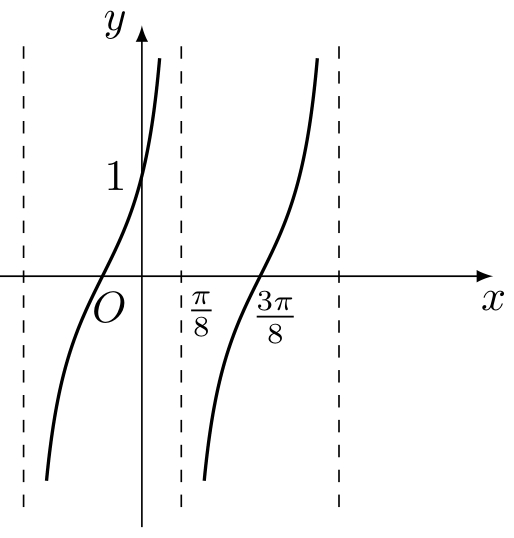
\includegraphics[width=7.4cm]{GaoKao/images/2011/liaoning_liberal/q12_fig1.png}
\end{center}

        {\centering\begin{tabular*}{\linewidth}{@{}@{\extracolsep{\fill}}llll@{}}
          \text{A. }\(2 + \sqrt{3}\)  &  \text{B. }\(\sqrt{3}\)  &  \text{C. }\(\frac{\sqrt{3}}{3}\)  &  \text{D. }\(2 - \sqrt{3}\)
        \end{tabular*}\par}

    \end{enumerate}

\end{description}

\begin{description}

    \item[二、填空题]

    \begin{enumerate}[leftmargin=5pt]

      \addtocounter{enumi}{+12}

        \item 已知圆 \(C\) 经过 \(A(5,1)\)，\(B(1,3)\) 两点，圆心在 \(x\) 轴上，则 \(C\) 的方程为\rule[-0.3ex]{3em}{0.4pt}.

        \item 调查了某地若干户家庭的年收入 \(x\)（单位：万元）和年饮食支出 \(y\)（单位：万元）. 调查显示年收入 \(x\) 与年饮食支出 \(y\) 具有线性相关关系，并由调查数据得到 \(y\) 对 \(x\) 的回归直线方程：\(\hat{y} = 0.254x + 0.321\). 由回归直线方程可知，家庭年收入每增加 \(1\) 万元，年饮食支出平均增加\rule[-0.3ex]{3em}{0.4pt} 万元.

        \item \(S_{n}\) 为等差数列 \(\{a_{n}\}\) 的前 \(n\) 项和，\(S_{2} = S_{6}\)，\(a_{4} = 1\)，则 \(a_{5} =\)\rule[-0.3ex]{3em}{0.4pt}.

        \item 已知函数 \(f(x) = {\mathrm{e}}^{x} - 2x + a\) 有零点，则 \(a\) 的取值范围是\rule[-0.3ex]{3em}{0.4pt}.

    \end{enumerate}

\end{description}

\begin{description}

    \item[三、解答题]

    \begin{enumerate}[leftmargin=5pt]

      \addtocounter{enumi}{+16}

        \item \(\triangle ABC\) 的三个内角 \(A\)，\(B\)，\(C\) 所对的边分别为 \(a\)，\(b\)，\(c\)，\(a \sin A \sin B + b \cos^{2} A = \sqrt{2}a\).
\begin{enumerate}
\item 求 \(\frac{b}{a}\)；
\item 若 \(c^{2} = b^{2} + \sqrt{3}a^{2}\)，求 \(B\).
\end{enumerate}

        \item 如图，四边形 \(ABCD\) 为正方形，\(QA \perp\) 平面 \(ABCD\)，\(PD \parallel QA\)，\(QA = AB = \frac{1}{2}PD\).
\begin{enumerate}
\item 证明：\(PQ \perp\) 平面 \(DCQ\)；
\item 求棱锥 \(Q-ABCD\) 的体积与棱锥 \(P-DCQ\) 的体积比值.
\end{enumerate}

\begin{center}
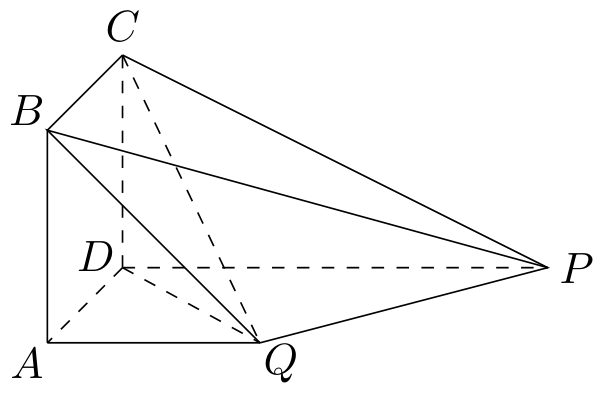
\includegraphics[width=7.2cm]{GaoKao/images/2011/liaoning_liberal/q18_fig1.png}
\end{center}

        \item 某农场计划种植某种新作物，为此对这种作物的两个品种（分别称为品种甲和品种乙）进行田间试验，选取两大块地. 每大块地分成 \(n\) 小块地. 在总共 \(2n\) 小块地中，随机选 \(n\) 小块地种植品种甲，另外 \(n\) 小块地种植品种乙.
\begin{enumerate}
\item 假设 \(n = 2\)，求第一大块地都种植品种甲的概率；
\item 试验时每大块地分成 \(8\) 小块，即 \(n = 8\)，试验结束后得到品种甲和品种乙在各小块地上的每公顷产量（单位：\(\mathrm{kg/hm^2}\)）如下表：
\begin{center}
\begin{tabular}{c|cccccccc}
\hline
品种甲 & \(403\) & \(397\) & \(390\) & \(404\) & \(388\) & \(400\) & \(412\) & \(406\) \\
\hline
品种乙 & \(419\) & \(403\) & \(412\) & \(418\) & \(408\) & \(423\) & \(400\) & \(413\) \\
\hline
\end{tabular}
\end{center}
分别求品种甲和品种乙每公顷产量的样本平均数和样本方差；根据试验结果，你应该种植哪一品种？
\end{enumerate}

附：样本数据 \(x_{1}\)，\(x_{2}\)，\(\cdots\)，\(x_{n}\) 的样本方差 \(s^{2} = \frac{1}{n}[(x_{1} - \overline{x})^{2} + (x_{2} - \overline{x})^{2} + \cdots + (x_{n} - \overline{x})^{2}]\)，其中 \(\overline{x}\) 为样本平均数.

        \item 设函数 \(f(x) = x + ax^{2} + b \ln x\)，曲线 \(y = f(x)\) 过 \(P(1,0)\)，且在 \(P\) 点处的切线斜率为 \(2\).
\begin{enumerate}
\item 求 \(a\)，\(b\) 的值；
\item 证明：\(f(x) \leqslant 2x - 2\).
\end{enumerate}

        \item 如图，已知椭圆 \(C_{1}\) 的中心在原点 \(O\)，长轴左，右端点 \(M\)，\(N\) 在 \(x\) 轴上，椭圆 \(C_{2}\) 的短轴为 \(MN\)，且 \(C_{1}\)，\(C_{2}\) 的离心率都为 \(e\). 直线 \(l \perp MN\)，\(l\) 与 \(C_{1}\) 交于两点，与 \(C_{2}\) 交于两点，这四点按纵坐标从大到小依次为 \(A\)，\(B\)，\(C\)，\(D\).
\begin{enumerate}
\item 设 \(e = \frac{1}{2}\)，求 \(|BC|\) 与 \(|AD|\) 的比值；
\item 当 \(e\) 变化时，是否存在直线 \(l\)，使得 \(BO \parallel AN\)，并说明理由.
\end{enumerate}

\begin{center}
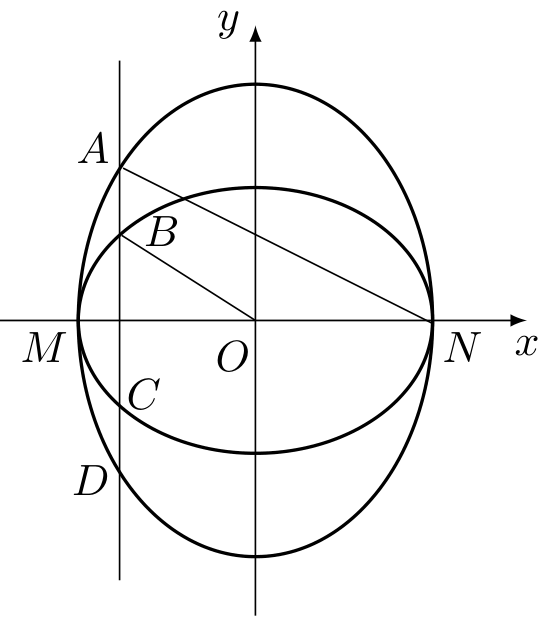
\includegraphics[width=2.0cm]{GaoKao/images/2011/liaoning_liberal/q21_fig1.png}
\end{center}

    \end{enumerate}

\end{description}

\begin{description}

    \item[四、选考题]

    \begin{enumerate}[leftmargin=5pt]

      \addtocounter{enumi}{+21}

        \item \textbf{【选修4-1：几何证明选讲】}

如图，\(A\)，\(B\)，\(C\)，\(D\) 四点在同一圆上，\(AD\) 的延长线与 \(BC\) 的延长线交于 \(E\) 点，且 \(EC = ED\).
\begin{enumerate}
\item 证明： \(CD \parallel AB\)；
\item 延长 \(CD\) 到 \(F\)，延长 \(DC\) 到 \(G\)，使得 \(EF = EG\)，证明： \(A\)，\(B\)，\(G\)，\(F\) 四点共圆.
\end{enumerate}

\begin{center}
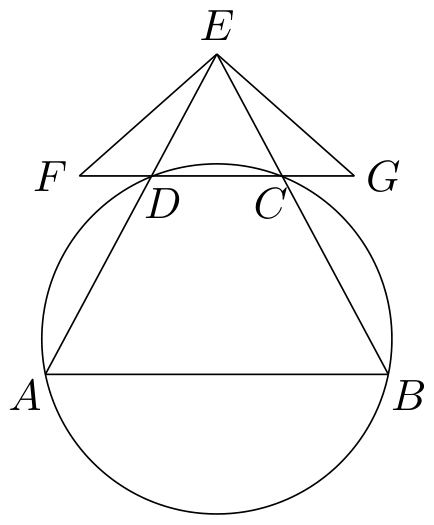
\includegraphics[width=5.4cm]{GaoKao/images/2011/liaoning_liberal/q22_fig1.png}
\end{center}

        \item \textbf{【选修4-4：坐标系与参数方程】}

在平面直角坐标系 \(xOy\) 中，曲线 \(C_{1}\) 的参数方程为 \(\begin{cases}
x = \cos \varphi,\\
y = \sin \varphi,
\end{cases}\)（\(\varphi\) 为参数）. 曲线 \(C_{2}\) 的参数方程为 \(\begin{cases}
x = a\cos \varphi,\\
y = b\sin \varphi,
\end{cases}\)（\(a > b > 0\)，\(\varphi\) 为参数）. 在以 \(O\) 为极点，\(x\) 轴的正半轴为极轴的极坐标系中，射线 \(l: \theta = \alpha\) 与 \(C_{1}\)，\(C_{2}\) 各有一个交点. 当 \(\alpha = 0\) 时，这两个交点间的距离为 \(2\)，当 \(\alpha = \frac{\pi}{2}\) 时，这两个交点重合.
\begin{enumerate}
\item 分别说明 \(C_{1}\)，\(C_{2}\) 是什么曲线，并求出 \(a\) 与 \(b\) 的值；
\item 设当 \(\alpha = \frac{\pi}{2}\) 时，\(l\) 与 \(C_{1}\)，\(C_{2}\) 的交点分别为 \(A_{1}\)，\(B_{1}\)，当 \(\alpha = -\frac{\pi}{4}\) 时，\(l\) 与 \(C_{1}\)，\(C_{2}\) 的交点分别为 \(A_{2}\)，\(B_{2}\)，求四边形 \(A_{1}A_{2}B_{2}B_{1}\) 的面积.
\end{enumerate}

        \item \textbf{【选修4-5：不等式选讲】}

已知函数 \(f(x) = |x - 2| - |x - 5|\).
\begin{enumerate}
\item 证明： \(-3 \leqslant f(x) \leqslant 3\)；
\item 求不等式 \(f(x) \geqslant x^{2} - 8x + 15\) 的解集.
\end{enumerate}

    \end{enumerate}

\end{description}


\subsection{2011年上海卷（理）}\label{gk:2011年上海卷（理）}

\begin{description}

    \item[一、填空题]

    \begin{enumerate}[leftmargin=5pt]

        \item 函数 \( f(x) = \frac{1}{x - 2} \) 的反函数为 \( f^{-1}(x) = \)\rule[-0.3ex]{3em}{0.4pt}.

        \item 若全集 \(U = \mathbb{R}\)，集合 \(A = \{x \mid x \geqslant 1\} \cup \{x \mid x \leqslant 0\}\)，则 \(\complement_U A =\rule[-0.3ex]{3em}{0.4pt}\).

        \item 设 \(m\) 为常数，若点 \(F(0,5)\) 是双曲线 \(\frac{y^2}{m} - \frac{x^2}{9} = 1\) 的一个焦点，则 \(m =\rule[-0.3ex]{3em}{0.4pt}\).

        \item 不等式 \(\frac{x + 1}{x} \leqslant 3\) 的解集为\rule[-0.3ex]{3em}{0.4pt}.

        \item 在极坐标系中，直线 \(\rho(2\cos \theta + \sin \theta) = 2\) 与直线 \(\rho\cos \theta = 1\) 的夹角大小为\rule[-0.3ex]{3em}{0.4pt}. （结果用反三角函数值表示）

        \item 在相距 2 千米的 \(A, B\) 两点处测量目标 \(C\)，若 \(\angle CAB = 75^{\circ}\)，\(\angle CBA = 60^{\circ}\)，则 \(A, C\) 两点之间的距离为\rule[-0.3ex]{3em}{0.4pt}\text{千米}.

        \item 若圆锥的侧面积为 \(2\pi\)，底面积为 \(\pi\)，则该圆锥的体积为\rule[-0.3ex]{3em}{0.4pt}.

        \item 函数 \( y = \sin \left(\frac{\pi}{2} + x\right) \cos \left(\frac{\pi}{6} - x\right) \) 的最大值为\rule[-0.3ex]{3em}{0.4pt}.

        \item 马老师从课本上抄录一个随机变量 \(\xi\) 的概率分布列如下表：

\begin{center}
\begin{tabular}{|c|c|c|c|}
\hline
\(X\) & 1 & 2 & 3 \\
\hline
\(P(\xi=x)\) & ? & ! & ? \\
\hline
\end{tabular}
\end{center}

请小牛同学计算 \( \xi \) 的数学期望，尽管“!”处无法完全看清，且两个“?”处字迹模糊，但能肯定这两个“?”处的数值相同. 据此，小牛给出了正确答案 \(E(\xi)=\)\rule[-0.3ex]{3em}{0.4pt}.

        \item 行列式 \(\begin{vmatrix}a & b\\ c & d \end{vmatrix}\) （\(a,b,c,d\in \{-1,1,2\}\)）所有可能的值中，最大的是\rule[-0.3ex]{3em}{0.4pt}.

        \item 在正三角形 \(ABC\) 中，\(D\) 是 \(BC\) 上的点. 若 \(AB = 3\)，\(BD = 1\)，则 \(\overrightarrow{AB} \cdot \overrightarrow{AD} =\rule[-0.3ex]{3em}{0.4pt}.\)

        \item 随机抽取的 9 位同学中，至少有 2 位同学在同一月份出生的概率为\rule[-0.3ex]{3em}{0.4pt}. （默认每个月的天数相同，结果精确到 0.001）

        \item 设 \(g(x)\) 是定义在 \(\mathbb{R}\) 上，以 1 为周期的函数，若函数 \(f(x) = x + g(x)\) 在区间 \([3,4]\) 上的值域为 \([-2,5]\)，则 \(f(x)\) 在区间 \([-10,10]\) 上的值域为\rule[-0.3ex]{3em}{0.4pt}.

        \item 已知点 \(O(0,0)\)，\(Q_0(0,1)\) 和点 \(R_0(3,1)\)，记 \(Q_0R_0\) 的中点为 \(P_1\)，取 \(Q_0P_1\) 和 \(P_1R_0\) 中的一条，记其端点为 \(Q_1\)，\(R_1\)，使之满足 \((|OQ_1| - 2)(|OR_1| - 2) < 0\)，记 \(Q_1R_1\) 的中点为 \(P_2\)，取 \(Q_1P_2\) 和 \(P_2R_1\) 中的一条，记其端点为 \(Q_2\)，\(R_2\)，使之满足 \((|OQ_2| - 2)(|OR_2| - 2) < 0\). 依次下去，得到 \(P_1\)，\(P_2\)，\(\cdots\)，\(P_n\)，\(\cdots\)，则 \(\lim\limits_{n \to \infty} \left|Q_0P_n\right| =\rule[-0.3ex]{3em}{0.4pt} \).

    \end{enumerate}

\end{description}

\begin{description}

    \item[二、选择题]

    \begin{enumerate}[leftmargin=5pt]

      \addtocounter{enumi}{+14}

        \item 若 \(a\)，\(b \in \mathbb{R}\)，且 \(ab > 0\)，则下列不等式中，恒成立的是（\quad）

        {\centering\begin{tabular*}{\linewidth}{@{}@{\extracolsep{\fill}}llll@{}}
          \text{A. }\(a^{2} + b^{2} > 2ab\)  &  \text{B. }\(a + b \geqslant 2\sqrt{ab}\)  &  \text{C. }\(\frac{1}{a} + \frac{1}{b} > \frac{2}{\sqrt{ab}}\)  &  \text{D. }\(\frac{b}{a} + \frac{a}{b} \geqslant 2\)
        \end{tabular*}\par}

        \item 下列函数中，既是偶函数，又是在区间 \((0,+\infty)\) 上单调递减的函数是（\quad）

        {\centering\begin{tabular*}{\linewidth}{@{}@{\extracolsep{\fill}}llll@{}}
          \text{A. }\(y = \ln \frac{1}{|x|}\)  &  \text{B. }\(y = x^{3}\)  &  \text{C. }\(y = 2^{|x|}\)  &  \text{D. }\(y = \cos x\)
        \end{tabular*}\par}

        \item 设 \(A_1\)，\(A_2\)，\(A_3\)，\(A_4\)，\(A_5\) 是平面上给定的 5 个不同点，则使 \(\overrightarrow{MA_1} + \overrightarrow{MA_2} + \overrightarrow{MA_3} + \overrightarrow{MA_4} + \overrightarrow{MA_5} = \vec{0}\) 成立的点 \(M\) 的个数为（\quad）

        {\centering\begin{tabular*}{\linewidth}{@{}@{\extracolsep{\fill}}llll@{}}
          \text{A. }\(0\)  &  \text{B. }\(1\)  &  \text{C. }\(5\)  &  \text{D. }\(10\)
        \end{tabular*}\par}

        \item 设 \(\{a_n\}\) 是各项为正数的无穷数列，\(A_i\) 是边长为 \(a_i\)，\(a_{i+1}\) 的矩形面积 （\(i = 1, 2, \cdots\)），则 \(\{A_n\}\) 为等比数列的充要条件为（\quad）

        {\centering\begin{tabular*}{\linewidth}{@{}@{\extracolsep{\fill}}llll@{}}
          \text{A. }\(\{a_n\}\) 是等比数列  &  \text{B. }\(\{a_1, a_3, \cdots, a_{2n-1}, \cdots\}\) 或 \(\{a_2, a_4, \cdots, a_{2n}, \cdots\}\) 是等比数列  &  \text{C. }\(\{a_1, a_3, \cdots, a_{2n-1}, \cdots\}\) 和 \(\{a_2, a_4, \cdots, a_{2n}, \cdots\}\) 均是等比数列  &  \text{D. }\(\{a_1, a_3, \cdots, a_{2n-1}, \cdots\}\) 和 \(\{a_2, a_4, \cdots, a_{2n}, \cdots\}\) 均是等比数列，且公比相同
        \end{tabular*}\par}

    \end{enumerate}

\end{description}

\begin{description}

    \item[三、解答题]

    \begin{enumerate}[leftmargin=5pt]

      \addtocounter{enumi}{+18}

        \item 已知复数 \(z_1\) 满足 \((z_1 - 2)(1 + \i) = 1 - \i\)（\(\i\) 为虚数单位），复数 \(z_2\) 的虚部为 2，且 \(z_1 \cdot z_2\) 是实数，求 \(z_2\).

        \item 已知函数 \(f(x) = a \cdot 2^{x} + b \cdot 3^{x}\)，其中常数 \(a\)，\(b\) 满足 \(a \cdot b \neq 0\).

\begin{enumerate}
\item 若 \(a \cdot b > 0\)，判断函数 \(f(x)\) 的单调性；
\item 若 \(a \cdot b < 0\)，求 \(f(x+1) > f(x)\) 时的 \(x\) 的取值范围.
\end{enumerate}

        \item 已知 \(ABCD - A_{1}B_{1}C_{1}D_{1}\) 是底面边长为 1 的正四棱柱，\(O_1\) 为 \(A_1C_1\) 与 \(B_1D_1\) 的交点.

\begin{enumerate}
\item 设 \(AB_1\) 与底面 \(A_1B_1C_1D_1\) 所成角的大小为 \(\alpha\)，二面角 \(A - B_{1}D_{1} - A_1\) 的大小为 \(\beta\). 求证：\(\tan \beta = \sqrt{2}\tan \alpha\)；
\item 若点 \(C\) 到平面 \(AB_1D_1\) 的距离为 \(\frac{4}{3}\)，求正四棱柱 \(ABCD - A_{1}B_{1}C_{1}D_{1}\) 的高.
\end{enumerate}

\begin{center}
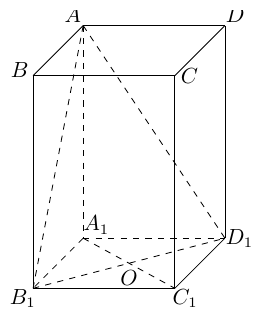
\includegraphics[width=5.3cm]{GaoKao/images/2011/shanghai_science/q21_fig1.png}
\end{center}

        \item 已知数列 \(\{a_n\}\) 和 \(\{b_n\}\) 的通项公式分别为 \(a_n = 3n + 6\)，\(b_n = 2n + 7\) （\(n \in \mathbf{N}^{*}\)），将集合 \(\{x \mid x = a_n, n \in \mathbf{N}^{*}\} \cup \{x \mid x = b_n, n \in \mathbf{N}^{*}\}\) 中的元素从小到大依次排列，构成数列 \(c_1\)，\(c_2\)，\(c_3\)，\(\cdots\)，\(c_n\)，\(\cdots\).

\begin{enumerate}
\item 求 \(c_1\)，\(c_2\)，\(c_3\)，\(c_4\)；
\item 求证：在数列 \(\{a_n\}\) 中，但不在数列 \(\{b_n\}\) 中的项恰为 \(a_2\)，\(a_4\)，\(\cdots\)，\(a_{2n}\)，\(\cdots\)；
\item 求数列 \(\{c_n\}\) 的通项公式.
\end{enumerate}

        \item 已知平面上的线段 \(l\) 及点 \(P\)，在 \(l\) 上任取一点 \(Q\)，线段 \(PQ\) 长度的最小值称为点 \(P\) 到线段 \(l\) 的距离，记作 \(d(P, l)\).

\begin{enumerate}
\item 求点 \(P(1,1)\) 到线段 \(l: x - y - 3 = 0\)（\(3 \leqslant x \leqslant 5\)）的距离 \(d(P, l)\)；
\item 设 \(l\) 是长为 2 的线段，求点的集合 \(D = \{P \mid d(P, l) \leqslant 1\}\) 所表示的图形面积；
\item 写出到两条线段 \(l_1\)，\(l_2\) 距离相等的点的集合 \(\Omega = \{P \mid d(P, l_1) = d(P, l_2)\}\)，其中 \(l_1 = AB\)，\(l_2 = CD\)，\(A\)，\(B\)，\(C\)，\(D\) 是下列三组点中的一组.

\begin{enumerate}
\item \(A(1,3)\)，\(B(1,0)\)，\(C(-1,3)\)，\(D(-1,0)\).
\item \(A(1,3)\)，\(B(1,0)\)，\(C(-1,3)\)，\(D(-1,-2)\).
\item \(A(0,1)\)，\(B(0,0)\)，\(C(0,0)\)，\(D(2,0)\).
\end{enumerate}
\end{enumerate}

    \end{enumerate}

\end{description}


\subsection{2011年上海卷（文）}\label{gk:2011年上海卷（文）}

\begin{description}

    \item[一、填空题]

    \begin{enumerate}[leftmargin=5pt]

        \item 若全集 \(U = \mathbb{R}\)，集合 \(A = \{x \mid x \geqslant 1\}\)，则 \(\complement_U A =\rule[-0.3ex]{3em}{0.4pt}\).

        \item \(\lim\limits_{n\to \infty}\left(1 - \frac{3n}{n + 3}\right) =\rule[-0.3ex]{3em}{0.4pt}\).

        \item 若函数 \( f(x) = 2x + 1 \) 的反函数为 \( f^{-1}(x) \)，则 \( f^{-1}(-2) = \)\rule[-0.3ex]{3em}{0.4pt}.

        \item 函数 \( y = 2\sin x - \cos x \) 的最大值为\rule[-0.3ex]{3em}{0.4pt}.

        \item 若直线 \(l\) 过点 \( (3,4) \)，且 \( (1,2) \) 是它的一个法向量，则直线 \(l\) 的方程为\rule[-0.3ex]{3em}{0.4pt}.

        \item 不等式 \(\frac{1}{x} < 1\) 的解集为\rule[-0.3ex]{3em}{0.4pt}.

        \item 若一个圆锥的主视图（如图所示）是边长为 \(3\)，\(3\)，\(2\) 的三角形，则该圆锥的侧面积为\rule[-0.3ex]{3em}{0.4pt}.
\begin{center}
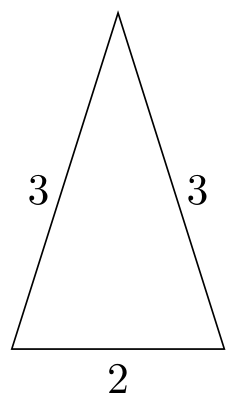
\includegraphics[width=2.3cm]{GaoKao/images/2011/shanghai_liberal/q7_fig1.png}
\end{center}

        \item 在相距 \(2\mathrm{~km}\) 的 \(A\)，\(B\) 两点处测量目标点 \(C\)，若 \(\angle CAB = 75^{\circ}\)，\(\angle CBA = 60^{\circ}\)，则 \(A\)，\(C\) 两点之间的距离是\rule[-0.3ex]{3em}{0.4pt}\(\mathrm{~km}\).

        \item 若变量 \(x\)，\(y\) 满足条件 \(\begin{cases}
3x - y \leqslant 0,\\
x - 3y + 5 \geqslant 0,
\end{cases}\) 则 \(z = x + y\) 的最大值为\rule[-0.3ex]{3em}{0.4pt}.

        \item 课题组进行城市空气质量调查，按地域把 \(24\) 个城市分成甲，乙，丙三组，对应的城市数分别为 \(4\)，\(12\)，\(8\)，若用分层抽样抽取 \(6\) 个城市，则丙组中应抽取的城市数为\rule[-0.3ex]{3em}{0.4pt}.

        \item 行列式 \(\begin{vmatrix}a & b\\ c & d \end{vmatrix}\) （\(a, b, c, d \in \{-1,1,2\}\)） 所有可能的值中，最大的是\rule[-0.3ex]{3em}{0.4pt}.

        \item 在正三角形 \(ABC\) 中，\(D\) 是 \(BC\) 上的点. 若 \(AB = 3\)，\(BD = 1\)，则 \(\overrightarrow{AB} \cdot \overrightarrow{AD} =\)\rule[-0.3ex]{3em}{0.4pt}.

        \item 随机抽取的 \(9\) 位同学中，至少有 \(2\) 位同学在同一月份出生的概率为\rule[-0.3ex]{3em}{0.4pt}（默认每个月的天数相同，结果精确到 \(0.001\)）.

        \item 设 \(g(x)\) 是定义在 \(\mathbb{R}\) 上，以 1 为周期的函数，若函数 \(f(x) = x + g(x)\) 在区间 \([0,1]\) 上的值域为 \([-2,5]\)，则 \(f(x)\) 在区间 \([0,3]\) 上的值域为\rule[-0.3ex]{3em}{0.4pt}.

    \end{enumerate}

\end{description}

\begin{description}

    \item[二、选择题]

    \begin{enumerate}[leftmargin=5pt]

      \addtocounter{enumi}{+14}

        \item 下列函数中，既是偶函数，又在区间 \((0, +\infty)\) 上单调递减的是（\quad）

        {\centering\begin{tabular*}{\linewidth}{@{}@{\extracolsep{\fill}}llll@{}}
          \text{A. }\( y = x^{-2} \)  &  \text{B. }\( y = x^{-1} \)  &  \text{C. }\( y = x^{2} \)  &  \text{D. }\( y = x^{\frac{1}{3}} \)
        \end{tabular*}\par}

        \item 若 \(a\)，\(b \in \mathbb{R}\)，且 \(ab > 0\)，则下列不等式中，恒成立的是（\quad）

        {\centering\begin{tabular*}{\linewidth}{@{}@{\extracolsep{\fill}}llll@{}}
          \text{A. }\(a^2 + b^2 > 2ab\)  &  \text{B. }\(a + b \geqslant 2\sqrt{ab}\)  &  \text{C. }\(\frac{1}{a} + \frac{1}{b} > \frac{2}{\sqrt{ab}}\)  &  \text{D. }\(\frac{b}{a} + \frac{a}{b} \geqslant 2\)
        \end{tabular*}\par}

        \item 若三角方程 \(\sin x = 0\) 与 \(\sin 2x = 0\) 的解集分别为 \(E\)，\(F\)，则（\quad）

        {\centering\begin{tabular*}{\linewidth}{@{}@{\extracolsep{\fill}}llll@{}}
          \text{A. }\(E \subsetneq F\)  &  \text{B. }\(E \supsetneq F\)  &  \text{C. }\(E = F\)  &  \text{D. }\(E \cap F = \varnothing\)
        \end{tabular*}\par}

        \item 设 \(A_{1}\)，\(A_{2}\)，\(A_{3}\)，\(A_{4}\) 是平面上给定的 4 个不同点，则使 \(\overrightarrow{MA_{1}} + \overrightarrow{MA_{2}} + \overrightarrow{MA_{3}} + \overrightarrow{MA_{4}} = \overrightarrow{0}\) 成立的点 \(M\) 的个数为（\quad）

        {\centering\begin{tabular*}{\linewidth}{@{}@{\extracolsep{\fill}}llll@{}}
          \text{A. }0  &  \text{B. }1  &  \text{C. }2  &  \text{D. }4
        \end{tabular*}\par}

    \end{enumerate}

\end{description}

\begin{description}

    \item[三、解答题]

    \begin{enumerate}[leftmargin=5pt]

      \addtocounter{enumi}{+18}

        \item 已知复数 \(z_{1}\) 满足 \((z_{1} - 2)(1 + \i) = 1 - \i\)（\(\i\) 为虚数单位），复数 \(z_{2}\) 的虚部为 2，且 \(z_{1} \cdot z_{2}\) 是实数，求 \(z_{2}\).

        \item 已知 \(ABCD - A_{1}B_{1}C_{1}D_{1}\) 是底面边长为 \(1\) 的正四棱柱，高 \(AA_{1} = 2\)，求：
\begin{enumerate}
\item 异面直线 \(BD\) 与 \(AB_{1}\) 所成角的余弦值；
\item 四面体 \(AB_{1}D_{1}C\) 的体积.
\end{enumerate}
\begin{center}
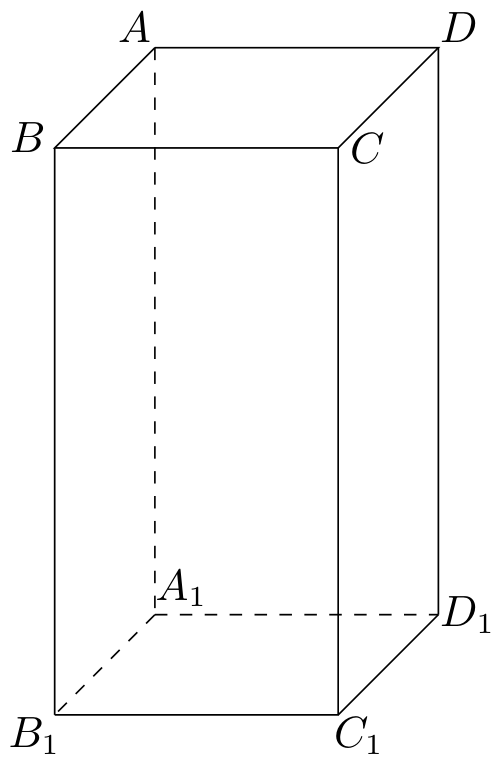
\includegraphics[width=5.0cm]{GaoKao/images/2011/shanghai_liberal/q20_fig1.png}
\end{center}

        \item 已知函数 \(f(x) = a \cdot 2^{x} + b \cdot 3^{x}\)，其中常数 \(a\)，\(b\) 满足 \(a \cdot b \neq 0\).
\begin{enumerate}
\item 若 \(a \cdot b > 0\)，判断函数 \(f(x)\) 的单调性；
\item 若 \(a \cdot b < 0\)，求 \(f(x + 1) > f(x)\) 时的 \(x\) 的取值范围.
\end{enumerate}

        \item 已知椭圆 \(C: \frac{x^2}{m^2} + y^{2} = 1\)（常数 \(m > 1\)），\(P\) 是曲线 \(C\) 上的动点，\(M\) 是曲线 \(C\) 的右顶点，定点 \(A\) 的坐标为 \((2,0)\).
\begin{enumerate}
\item 若 \(M\) 与 \(A\) 重合，求曲线 \(C\) 的焦点坐标；
\item 若 \(m = 3\)，求 \(|PA|\) 的最大值与最小值；
\item 若 \(|PA|\) 的最小值为 \(|MA|\)，求实数 \(m\) 的取值范围.
\end{enumerate}

        \item 已知数列 \(\{a_{n}\}\) 和 \(\{b_{n}\}\) 的通项公式分别为 \(a_{n} = 3n + 6\)，\(b_{n} = 2n + 7\)（\(n \in \mathbf{N}^{*}\)），将集合 \(\{x \mid x = a_{n}, n \in \mathbf{N}^{*}\} \cup \{x \mid x = b_{n}, n \in \mathbf{N}^{*}\}\) 中的元素从小到大依次排列，构成数列 \(c_{1}\)，\(c_{2}\)，\(c_{3}\)，\(\cdots\)，\(c_{n}\)，\(\cdots\).
\begin{enumerate}
\item 求三个最小的数，使它们既是数列 \(\{a_{n}\}\) 中的项，又是数列 \(\{b_{n}\}\) 中的项；
\item 数列 \(c_{1}\)，\(c_{2}\)，\(c_{3}\)，\(\cdots\)，\(c_{40}\) 中有多少项不是数列 \(\{b_{n}\}\) 中的项？请说明理由；
\item 求数列 \(\{c_{n}\}\) 的前 \(4n\) 项和 \(S_{4n}\)（\(n \in \mathbf{N}^{*}\)）.
\end{enumerate}

    \end{enumerate}

\end{description}


\subsection{2011年四川卷（理）}\label{gk:2011年四川卷（理）}

\begin{description}

    \item[一、选择题]

    \begin{enumerate}[leftmargin=5pt]

        \item 有一个容量为 66 的样本，数据的分组及各组的频数如下：
\begin{center}
\begin{tabular}{cccc}
\([11.5,15.5)\) & \([15.5,19.5)\) & \([19.5,23.5)\) & \([23.5,27.5)\)\\
2 & 4 & 9 & 18\\
\([27.5,31.5)\) & \([31.5,35.5)\) & \([35.5,39.5)\) & \([39.5,43.5)\)\\
11 & 12 & 7 & 3
\end{tabular}
\end{center}
根据样本的频率分布，估计数据落在 \([31.5,43.5)\) 的概率约是（\quad）

        {\centering\begin{tabular*}{\linewidth}{@{}@{\extracolsep{\fill}}llll@{}}
          \text{A. }\(\frac{1}{6}\)  &  \text{B. }\(\frac{1}{3}\)  &  \text{C. }\(\frac{1}{2}\)  &  \text{D. }\(\frac{2}{3}\)
        \end{tabular*}\par}

        \item 复数 \(-\i + \frac{1}{\i} =\)（\quad）

        {\centering\begin{tabular*}{\linewidth}{@{}@{\extracolsep{\fill}}llll@{}}
          \text{A. }\(-2\i\)  &  \text{B. }\(\frac{1}{2}\i\)  &  \text{C. }0  &  \text{D. }\(2\i\)
        \end{tabular*}\par}

        \item \(l_{1}\)，\(l_{2}\)，\(l_{3}\) 是空间三条不同的直线，则下列命题正确的是（\quad）

        {\centering\begin{tabular*}{\linewidth}{@{}@{\extracolsep{\fill}}llll@{}}
          \text{A. }\(l_{1} \perp l_{2}, l_{2} \perp l_{3} \Rightarrow l_{1} \parallel l_{3}\)  &  \text{B. }\(l_{1} \perp l_{2}\)，\(l_{2} \parallel l_{3} \Rightarrow l_{1} \perp l_{3}\)  &  \text{C. }\(l_{1} \parallel l_{2} \parallel l_{3} \Rightarrow l_{1}\)，\(l_{2}\)，\(l_{3}\) 共面  &  \text{D. }\(l_{1}\)，\(l_{2}\)，\(l_{3}\) 共点 \(\Rightarrow l_{1}\)，\(l_{2}\)，\(l_{3}\) 共面
        \end{tabular*}\par}

        \item 如图，正六边形 \(ABCDEF\) 中，\(\overrightarrow{BA} + \overrightarrow{CD} + \overrightarrow{EF} =\)（\quad）

\begin{center}
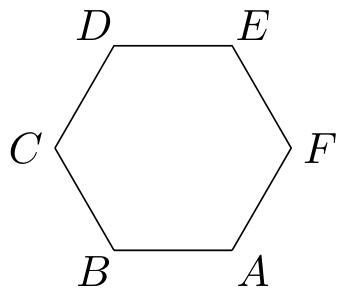
\includegraphics[width=4.3cm]{GaoKao/images/2011/sichuan_science/q4_fig1.png}
\end{center}

        {\centering\begin{tabular*}{\linewidth}{@{}@{\extracolsep{\fill}}llll@{}}
          \text{A. }0  &  \text{B. }\(\overrightarrow{BE}\)  &  \text{C. }\(\overrightarrow{AD}\)  &  \text{D. }\(\overrightarrow{CF}\)
        \end{tabular*}\par}

        \item “函数 \(f(x)\) 在点 \(x = x_0\) 处有定义”是“\(f(x)\) 在点 \(x = x_0\) 处连续”的（\quad）

        {\centering\begin{tabular*}{\linewidth}{@{}@{\extracolsep{\fill}}llll@{}}
          \text{A. }充分而不必要的条件  &  \text{B. }必要而不充分的条件  &  \text{C. }充要条件  &  \text{D. }既不充分也不必要的条件
        \end{tabular*}\par}

        \item 在 \(\triangle ABC\) 中，\(\sin^2 A \leqslant \sin^2 B + \sin^2 C - \sin B \sin C\)，则 \(A\) 的取值范围是（\quad）

        {\centering\begin{tabular*}{\linewidth}{@{}@{\extracolsep{\fill}}llll@{}}
          \text{A. }\(\left(0, \frac{\pi}{6}\right]\)  &  \text{B. }\(\left[\frac{\pi}{6},\pi\right)\)  &  \text{C. }\(\left(0, \frac{\pi}{3}\right]\)  &  \text{D. }\(\left[\frac{\pi}{3}, \pi\right)\)
        \end{tabular*}\par}

        \item 已知 \( f(x) \) 是 \( \mathbb{R} \) 上的奇函数，且当 \( x > 0 \) 时，\( f(x) = \left(\frac{1}{2}\right)^x + 1 \)，则 \( f(x) \) 的反函数的图象大致是（\quad）

        {\centering\begin{tabular*}{\linewidth}{@{}@{\extracolsep{\fill}}cccc@{}}
          \text{A. }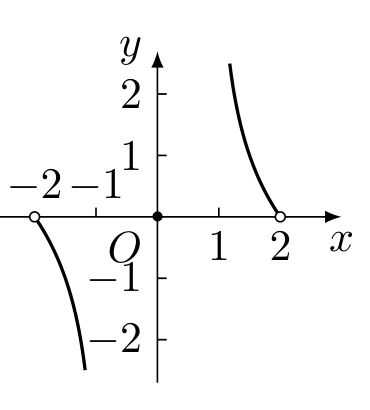
\includegraphics[width=0.15\paperwidth]{GaoKao/images/2011/sichuan_science/q7_choice_a.png}  &  \text{B. }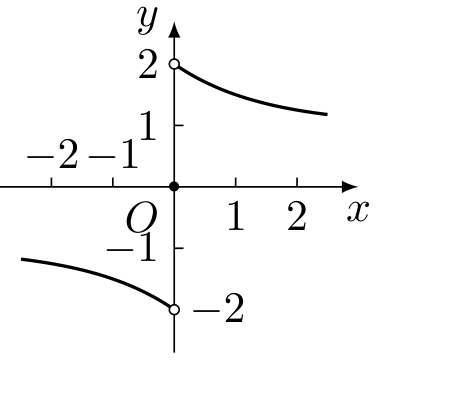
\includegraphics[width=0.15\paperwidth]{GaoKao/images/2011/sichuan_science/q7_choice_b.png}  &  \text{C. }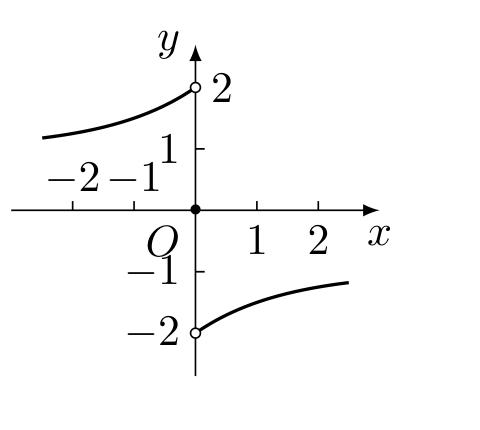
\includegraphics[width=0.15\paperwidth]{GaoKao/images/2011/sichuan_science/q7_choice_c.png}  &  \text{D. }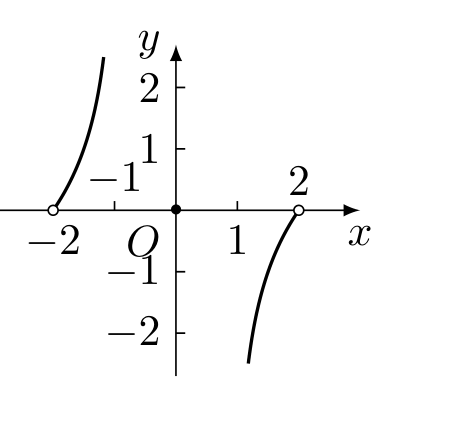
\includegraphics[width=0.15\paperwidth]{GaoKao/images/2011/sichuan_science/q7_choice_d.png}
        \end{tabular*}\par}

        \item 数列 \( \{a_{n}\} \) 的首项为 3，\( \{b_{n}\} \) 为等差数列且 \( b_{n}=a_{n+1}-a_{n} \)（\( n\in \mathbb{N}^{*} \)）. 若 \( b_{3}=-2 \)，\( b_{10}=12 \)，则 \( a_{8} =\)（\quad）

        {\centering\begin{tabular*}{\linewidth}{@{}@{\extracolsep{\fill}}llll@{}}
          \text{A. }0  &  \text{B. }3  &  \text{C. }8  &  \text{D. }11
        \end{tabular*}\par}

        \item 某运输公司有 12 名驾驶员和 19 名工人，有 8 辆载重量为 10 吨的甲型卡车和 7 辆载重量为 6 吨的乙型卡车. 某天需运往 \(A\) 地至少 72 吨的货物，派用的每辆车需载满且只能送一次，派用的每辆甲型卡车需配 2 名工人，运送一次可得利润 450 元；派用的每辆乙型卡车需配 1 名工人，运送一次可得利润 350 元. 该公司合理计划当天派用甲，乙卡车的车辆数，可得最大利润 \(z =\)（\quad）

        {\centering\begin{tabular*}{\linewidth}{@{}@{\extracolsep{\fill}}llll@{}}
          \text{A. }4650 元  &  \text{B. }4700 元  &  \text{C. }4900 元  &  \text{D. }5000 元
        \end{tabular*}\par}

        \item 在抛物线 \( y = x^{2} + ax - 5\) （\(a \neq 0\)）上取横坐标为 \(x_{1} = -4\)，\(x_{2} = 2\) 的两点，经过两点引一条割线，有平行于该割线的一条直线同时与抛物线和圆 \( 5x^{2} + 5y^{2} = 36 \) 相切，则抛物线顶点的坐标为（\quad）

        {\centering\begin{tabular*}{\linewidth}{@{}@{\extracolsep{\fill}}llll@{}}
          \text{A. }\((-2, -9)\)  &  \text{B. }\((0, -5)\)  &  \text{C. }\((2, -9)\)  &  \text{D. }\((1, -6)\)
        \end{tabular*}\par}

        \item 已知定义在 \( [0, +\infty) \) 上的函数 \( f(x) \) 满足 \( f(x) = 3f(x + 2) \)，当 \( x \in [0, 2) \) 时，\( f(x) = -x^{2} + 2x \). 设 \( f(x) \) 在 \( [2n - 2, 2n) \) 上的最大值为 \( a_{n} \) （\( n \in \mathbf{N}^{*} \)），且 \(\{a_{n}\}\) 的前 \(n\) 项和为 \(S_{n}\)，则 \(\lim\limits_{n\to\infty} S_{n} =\)（\quad）

        {\centering\begin{tabular*}{\linewidth}{@{}@{\extracolsep{\fill}}llll@{}}
          \text{A. }3  &  \text{B. }\(\frac{5}{2}\)  &  \text{C. }2  &  \text{D. }\(\frac{3}{2}\)
        \end{tabular*}\par}

        \item 在集合 \(\{1, 2, 3, 4, 5\}\) 中任取一个偶数 \(a\) 和一个奇数 \(b\) 构成以原点为起点的向量 \(\alpha = (a,b)\). 从所有得到的以原点为起点的向量中任取两个向量作为邻边作平行四边形. 记所有作成的平行四边形的个数为 \(n\)，其中面积不超过 4 的平行四边形的个数为 \(m\)，则 \(\frac{m}{n}=\)（\quad）

        {\centering\begin{tabular*}{\linewidth}{@{}@{\extracolsep{\fill}}llll@{}}
          \text{A. }\(\frac{4}{15}\)  &  \text{B. }\(\frac{1}{3}\)  &  \text{C. }\(\frac{2}{5}\)  &  \text{D. }\(\frac{2}{3}\)
        \end{tabular*}\par}

    \end{enumerate}

\end{description}

\begin{description}

    \item[二、填空题]

    \begin{enumerate}[leftmargin=5pt]

      \addtocounter{enumi}{+12}

        \item 计算 \(\left(\lg \frac{1}{4} - \lg 25\right) \div 100^{-\frac{1}{2}} =\rule[-0.3ex]{3em}{0.4pt}\).

        \item 双曲线 \(\frac{x^2}{64} - \frac{y^2}{36} = 1\) 上一点 \(P\) 到双曲线右焦点的距离是 4，那么点 \(P\) 到左准线的距离是\rule[-0.3ex]{3em}{0.4pt}.

        \item 如图，半径为 \(R\) 的球 \(O\) 中有一内接圆柱. 当圆柱的侧面积最大时，球的表面积与该圆柱的侧面积之差是\rule[-0.3ex]{3em}{0.4pt}.

\begin{center}
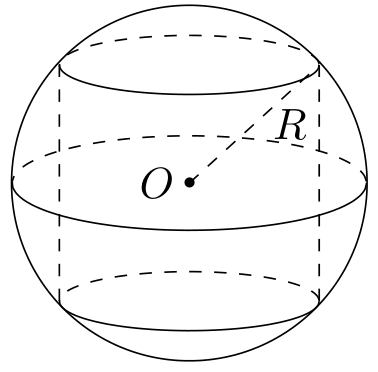
\includegraphics[width=4.4cm]{GaoKao/images/2011/sichuan_science/q15_fig1.png}
\end{center}

        \item 函数 \( f(x) \) 的定义域为 \(A\). 若 \(x_{1}\)，\(x_{2} \in A\) 且 \( f(x_{1}) = f(x_{2}) \) 时总有 \( x_{1} = x_{2} \)，则称 \( f(x) \) 为单函数. 例如，函数 \( f(x) = 2x + 1\) （\(x \in \mathbb{R}\)） 是单函数. 下列命题：
\begin{enumerate}
\item 函数 \( f(x)=x^{2} \)（\(x\in\mathbb{R}\)）是单函数；
\item 若 \(f(x)\) 为单函数，\(x_{1}\)，\(x_{2} \in A\) 且 \(x_{1} \neq x_{2}\)，则 \(f(x_{1}) \neq f(x_{2})\)；
\item 若 \(f: A \to B\) 为单函数，则对于任意 \(b \in B\)，它至多有一个原象；
\item 函数 \(f(x)\) 在某区间上具有单调性，
\end{enumerate}
则 \(f(x)\) 一定是单函数. 其中的真命题是\rule[-0.3ex]{3em}{0.4pt}.（写出所有真命题的编号）

    \end{enumerate}

\end{description}

\begin{description}

    \item[三、解答题]

    \begin{enumerate}[leftmargin=5pt]

      \addtocounter{enumi}{+16}

        \item 已知函数 \(f(x) = \sin \left( x + \frac{7\pi}{4} \right) + \cos \left( x - \frac{3\pi}{4} \right)\)，\(x \in \mathbb{R}\).
\begin{enumerate}
\item 求 \( f(x) \) 的最小正周期和最小值；
\item 已知 \(\cos(\beta-\alpha)=\frac{4}{5}\)，\(\cos(\beta+\alpha)=-\frac{4}{5}\)，\(0 < \alpha < \beta \leqslant \frac{\pi}{2}\)，求证： \(\left[f(\beta)\right]^2 - 2 = 0.\)
\end{enumerate}

        \item 本着健康，低碳的生活理念，租自行车骑游的人越来越多. 某自行车租车点的收费标准是每车每次租车时间不超过两小时免费，超过两小时的部分每小时收费 2 元（不足 1 小时的部分按 1 小时计算）. 有甲，乙两人相互独立来该租车点租车骑游（各租一车一次）. 设甲，乙不超过两小时还车的概率分别为 \(\frac{1}{4}\)，\(\frac{1}{2}\)；两小时以上且不超过三小时还车的概率分别是 \(\frac{1}{2}\)，\(\frac{1}{4}\)；两人租车时间都不会超过四小时.
\begin{enumerate}
\item 求甲，乙两人所付的租车费用相同的概率；
\item 设甲，乙两人所付的租车费用之和为随机变量 \(\xi\)，求 \(\xi\) 的分布列及数学期望 \(E(\xi)\).
\end{enumerate}

        \item 如图，在直三棱柱 \(ABC - A_{1}B_{1}C_{1}\) 中，\(\angle BAC = 90^{\circ}\)，\(AB = AC = AA_{1} = 1\). \(D\) 是棱 \(CC_{1}\) 上的一点，\(P\) 是 \(AD\) 的延长线与 \(A_{1}C_{1}\) 的延长线的交点，且 \(PB_{1} \parallel\) 平面 \(BDA_{1}\).
\begin{enumerate}
\item 求证： \(CD = C_{1}D\)；
\item 求二面角 \(A - A_{1}D - B\) 的平面角的余弦值；
\item 求点 \(C\) 到平面 \(B_{1}DP\) 的距离.
\end{enumerate}

\begin{center}
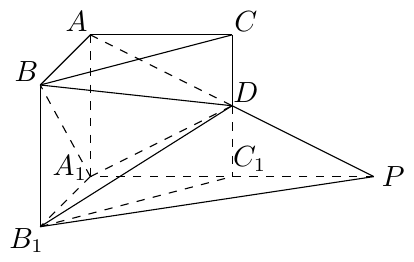
\includegraphics[width=3.4cm]{GaoKao/images/2011/sichuan_science/q19_fig1.png}
\end{center}

        \item 设 \(d\) 为非零实数，\(a_{n} = \frac{1}{n}\left[\mathrm{C}_{n}^{1}d + 2\mathrm{C}_{n}^{2}d^{2} + \dots + (n - 1)\mathrm{C}_{n}^{n - 1}d^{n - 1} + n\mathrm{C}_{n}^{n}d^{n}\right]\) （\(n\in \mathbf{N}^{*}\)）.
\begin{enumerate}
\item 写出 \(a_1\)，\(a_2\)，\(a_3\) 并判断 \(\{a_n\}\) 是否为等比数列. 若是，给出证明；若不是，说明理由；
\item 设 \( b_n = nda_n \) （\( n \in \mathbf{N}^* \)），求数列 \( \{b_n\} \) 的前 \( n \) 项和 \( S_n \).
\end{enumerate}

        \item 椭圆有两顶点 \(A(-1,0)\)，\(B(1,0)\)，过其焦点 \(F(0,1)\) 的直线 \(l\) 与椭圆交于 \(C\)，\(D\) 两点，并与 \(x\) 轴交于点 \(P\). 直线 \(AC\) 与直线 \(BD\) 交于点 \(Q\).
\begin{enumerate}
\item 当 \(|CD| = \frac{3}{2}\sqrt{2}\) 时，求直线 \(l\) 的方程.
\item 当点 \(P\) 异于 \(A\)，\(B\) 两点时，求证： \(\overrightarrow{OP} \cdot \overrightarrow{OQ}\) 为定值.
\end{enumerate}

\begin{center}
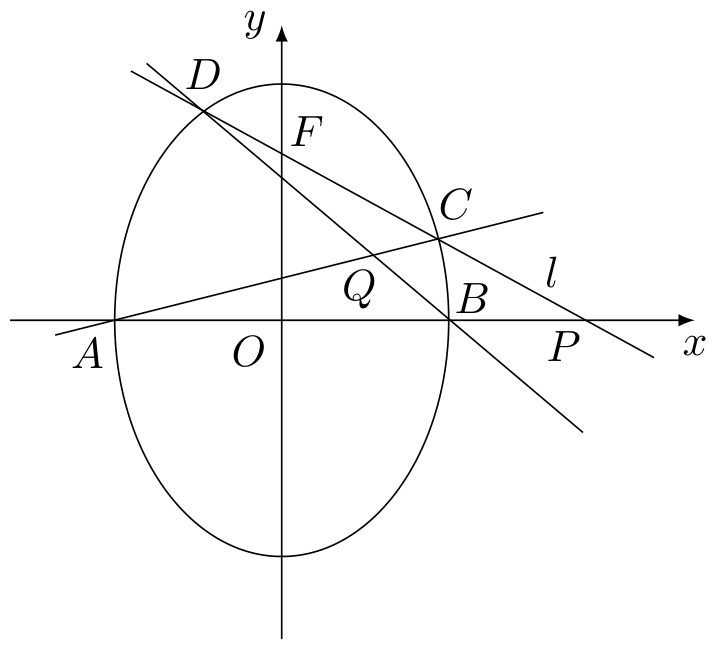
\includegraphics[width=8.9cm]{GaoKao/images/2011/sichuan_science/q21_fig1.png}
\end{center}

        \item 已知函数 \(f(x)=\frac{2}{3}x+\frac{1}{2}\)，\(h(x)=\sqrt{x}\).
\begin{enumerate}
\item 设函数 \(F(x)=f(x)-h(x)\)，求 \(F(x)\) 的单调区间与极值；
\item 设 \(a\in\mathbb{R}\)，解关于 \(x\) 的方程 \(\log_{4}\left[\frac{3}{2}f(x-1)-\frac{3}{4}\right]=\log_{2}h(a-x)-\log_{2}h(4-x)\)；
\item 试比较 \(f(100)h(100)-\displaystyle\sum_{k=1}^{100}h(k)\) 与 \(\frac{1}{6}\) 的大小.
\end{enumerate}

    \end{enumerate}

\end{description}


\subsection{2011年四川卷（文）}\label{gk:2011年四川卷（文）}

\begin{description}

    \item[一、选择题]

    \begin{enumerate}[leftmargin=5pt]

        \item 若全集 \(M = \{1, 2, 3, 4, 5\}\)，\(N = \{2, 4\}\)，则 \(\complement_{M}N =\)（\quad）

        {\centering\begin{tabular*}{\linewidth}{@{}@{\extracolsep{\fill}}llll@{}}
          \text{A. }\(\varnothing\)  &  \text{B. }\(\{1, 3, 5\}\)  &  \text{C. }\(\{2, 4\}\)  &  \text{D. }\(\{1, 2, 3, 4, 5\}\)
        \end{tabular*}\par}

        \item 有一容量为 \(66\) 的样本，数据的分组及各组的频数如下：
\begin{center}
\resizebox{\linewidth}{!}{%
\begin{tabular}{|c|c|c|c|c|c|c|c|}
\hline
\([11.5, 15.5)\) & \([15.5, 19.5)\) & \([19.5, 23.5)\) & \([23.5, 27.5)\) & \([27.5, 31.5)\) & \([31.5, 35.5)\) & \([35.5, 39.5)\) & \([39.5, 43.5)\) \\
\hline
2 & 4 & 9 & 18 & 11 & 12 & 7 & 3 \\
\hline
\end{tabular}%
}
\end{center}
根据样本的频率分布估计，大于或等于 \(31.5\) 的数据约占（\quad）

        {\centering\begin{tabular*}{\linewidth}{@{}@{\extracolsep{\fill}}llll@{}}
          \text{A. }\(\frac{2}{11}\)  &  \text{B. }\(\frac{1}{3}\)  &  \text{C. }\(\frac{1}{2}\)  &  \text{D. }\(\frac{2}{3}\)
        \end{tabular*}\par}

        \item 圆 \(x^2 + y^2 - 4x + 6y = 0\) 的圆心坐标是（\quad）

        {\centering\begin{tabular*}{\linewidth}{@{}@{\extracolsep{\fill}}llll@{}}
          \text{A. }\((2, 3)\)  &  \text{B. }\((-2, 3)\)  &  \text{C. }\((-2, -3)\)  &  \text{D. }\((2, -3)\)
        \end{tabular*}\par}

        \item 函数 \(y = \left(\frac{1}{2}\right)^x + 1\) 的图象关于直线 \(y = x\) 对称的图象大致是（\quad）

        {\centering\begin{tabular*}{\linewidth}{@{}@{\extracolsep{\fill}}cccc@{}}
          \text{A. }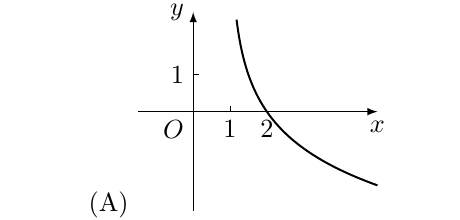
\includegraphics[width=0.15\paperwidth]{GaoKao/images/2011/sichuan_liberal/q4_choice_a.png}  &  \text{B. }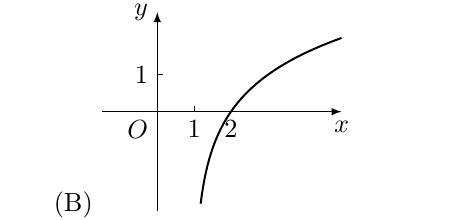
\includegraphics[width=0.15\paperwidth]{GaoKao/images/2011/sichuan_liberal/q4_choice_b.png}  &  \text{C. }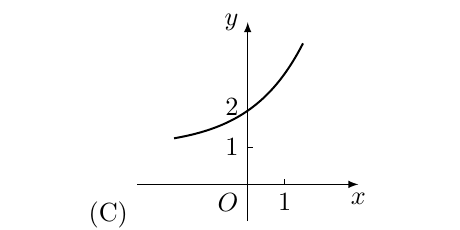
\includegraphics[width=0.15\paperwidth]{GaoKao/images/2011/sichuan_liberal/q4_choice_c.png}  &  \text{D. }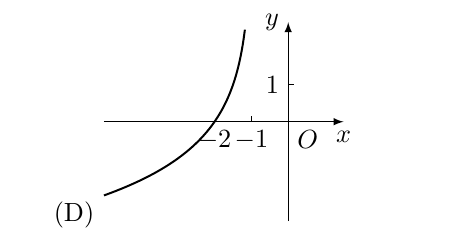
\includegraphics[width=0.15\paperwidth]{GaoKao/images/2011/sichuan_liberal/q4_choice_d.png}
        \end{tabular*}\par}

        \item “\(x = 3\)”是“\(x^2 = 9\)”的（\quad）

        {\centering\begin{tabular*}{\linewidth}{@{}@{\extracolsep{\fill}}llll@{}}
          \text{A. }充分而不必要的条件  &  \text{B. }必要而不充分的条件  &  \text{C. }充要条件  &  \text{D. }既不充分也不必要的条件
        \end{tabular*}\par}

        \item \(l_1\)，\(l_2\)，\(l_3\) 是空间三条不同的直线，则下列命题正确的是（\quad）

        {\centering\begin{tabular*}{\linewidth}{@{}@{\extracolsep{\fill}}llll@{}}
          \text{A. }\(l_1 \perp l_2, l_2 \perp l_3 \Rightarrow l_1 \parallel l_3\)  &  \text{B. }\(l_1 \perp l_2\)，\(l_2 \parallel l_3 \Rightarrow l_1 \perp l_3\)  &  \text{C. }\(l_1 \parallel l_2 \parallel l_3 \Rightarrow l_1\)，\(l_2\)，\(l_3\) 共面  &  \text{D. }\(l_1\)，\(l_2\)，\(l_3\) 共点 \(\Rightarrow l_1\)，\(l_2\)，\(l_3\) 共面
        \end{tabular*}\par}

        \item 如图，正六边形 \(ABCDEF\) 中，\(\overrightarrow{BA} + \overrightarrow{CD} + \overrightarrow{EF} =\)（\quad）

\begin{center}
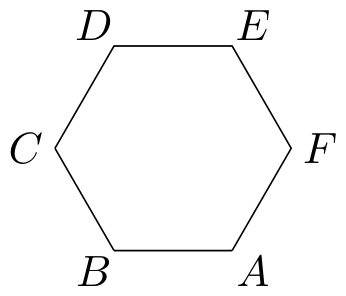
\includegraphics[width=4.3cm]{GaoKao/images/2011/sichuan_liberal/q7_fig1.png}
\end{center}

        {\centering\begin{tabular*}{\linewidth}{@{}@{\extracolsep{\fill}}llll@{}}
          \text{A. }\(0\)  &  \text{B. }\(\overrightarrow{BE}\)  &  \text{C. }\(\overrightarrow{AD}\)  &  \text{D. }\(\overrightarrow{CF}\)
        \end{tabular*}\par}

        \item 在 \(\triangle ABC\) 中，\(\sin^2 A \leqslant \sin^2 B + \sin^2 C - \sin B \sin C\)，则 \(A\) 的取值范围是（\quad）

        {\centering\begin{tabular*}{\linewidth}{@{}@{\extracolsep{\fill}}llll@{}}
          \text{A. }\((0, \frac{\pi}{6}]\)  &  \text{B. }\([\frac{\pi}{6}, \pi)\)  &  \text{C. }\((0, \frac{\pi}{3}]\)  &  \text{D. }\([\frac{\pi}{3}, \pi)\)
        \end{tabular*}\par}

        \item 数列 \(\{a_n\}\) 的前 \(n\) 项和为 \(S_n\)，若 \(a_1 = 1\)，\(a_{n+1} = 3S_n\)（\(n \geqslant 1\)），则 \(a_6 =\)（\quad）

        {\centering\begin{tabular*}{\linewidth}{@{}@{\extracolsep{\fill}}llll@{}}
          \text{A. }\(3 \times 4^4\)  &  \text{B. }\(3 \times 4^4 + 1\)  &  \text{C. }\(4^5\)  &  \text{D. }\(4^5 + 1\)
        \end{tabular*}\par}

        \item 某运输公司有 \(12\) 名驾驶员和 \(19\) 名工人，有 \(8\) 辆载重量为 \(10\text{ 吨}\) 的甲型卡车和 \(7\) 辆载重量为 \(6\text{ 吨}\) 的乙型卡车. 某天需运往 \(A\) 地至少 \(72\text{ 吨}\) 的货物，派用的每辆车需载满且只运送一次，派用的每辆甲型卡车需配 \(2\) 名工人，运送一次可得利润 \(450\text{ 元}\)；派用的每辆乙型卡车需配 \(1\) 名工人，运送一次可得利润 \(350\text{ 元}\)，该公司合理计划当天派用甲、乙卡车的车辆数，可得最大利润 \(z =\)（\quad）

        {\centering\begin{tabular*}{\linewidth}{@{}@{\extracolsep{\fill}}llll@{}}
          \text{A. }\(4650\text{ 元}\)  &  \text{B. }\(4700\text{ 元}\)  &  \text{C. }\(4900\text{ 元}\)  &  \text{D. }\(5000\text{ 元}\)
        \end{tabular*}\par}

        \item 在抛物线 \(y = x^2 + ax - 5\)（\(a \neq 0\)） 上取横坐标为 \(x_1 = -4\)，\(x_2 = 2\) 的两点，经过两点引一条割线，有平行于该割线的一条直线同时与抛物线和圆 \(5x^2 + 5y^2 = 36\) 相切，则抛物线顶点的坐标为（\quad）

        {\centering\begin{tabular*}{\linewidth}{@{}@{\extracolsep{\fill}}llll@{}}
          \text{A. }\((-2, -9)\)  &  \text{B. }\((0, -5)\)  &  \text{C. }\((2, -9)\)  &  \text{D. }\((1, -6)\)
        \end{tabular*}\par}

        \item 在集合 \(\{1, 2, 3, 4, 5\}\) 中任取一个偶数 \(a\) 和一个奇数 \(b\) 构成以原点为起点的向量 \(\alpha = (a, b)\). 从所有得到的以原点为起点的向量中任取两个向量为邻边作平行四边形，记所有作成的平行四边形的个数为 \(n\)，其中面积等于 2 的平行四边形的个数为 \(m\)，则 \(\frac{m}{n} =\)（\quad）

        {\centering\begin{tabular*}{\linewidth}{@{}@{\extracolsep{\fill}}llll@{}}
          \text{A. }\(\frac{2}{15}\)  &  \text{B. }\(\frac{1}{5}\)  &  \text{C. }\(\frac{4}{15}\)  &  \text{D. }\(\frac{1}{3}\)
        \end{tabular*}\par}

    \end{enumerate}

\end{description}

\begin{description}

    \item[二、填空题]

    \begin{enumerate}[leftmargin=5pt]

      \addtocounter{enumi}{+12}

        \item \((x + 1)^9\) 的展开式中 \(x^3\) 的系数是\rule[-0.3ex]{3em}{0.4pt}（用数字作答）

        \item 双曲线 \(\frac{x^2}{64} - \frac{y^2}{36} = 1\) 上一点 \(P\) 到双曲线右焦点的距离是 \(4\)，那么点 \(P\) 到左准线的距离是\rule[-0.3ex]{3em}{0.4pt}.

        \item 如图，半径为 \(4\) 的球 \(O\) 中有一内接圆柱. 当圆柱的侧面积最大时，球的表面积与该圆柱的侧面积之差是\rule[-0.3ex]{3em}{0.4pt}.

\begin{center}
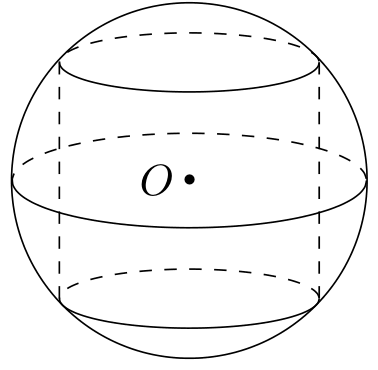
\includegraphics[width=3.4cm]{GaoKao/images/2011/sichuan_liberal/q15_fig1.png}
\end{center}

        \item 函数 \(f(x)\) 的定义域为 \(A\)，若 \(x_1\)，\(x_2 \in A\) 且 \(f(x_1) = f(x_2)\) 时总有 \(x_1 = x_2\)，则称 \(f(x)\) 为单函数. 例如，函数 \(f(x) = 2x + 1\)（\(x \in \mathbb{R}\)）是单函数. 下列命题：

\begin{enumerate}
\item \(f(x) = x^2\)（\(x \in \mathbb{R}\)）是单函数；
\item \(f(x) = 2^x\)（\(x \in \mathbb{R}\)）是单函数；
\item 若 \(f(x)\) 为单函数，\(x_1\)，\(x_2 \in A\) 且 \(x_1 \neq x_2\)，则 \(f(x_1) \neq f(x_2)\)；
\item 在定义域上具有单调性的函数一定是单函数.
\end{enumerate}

其中的真命题是\rule[-0.3ex]{3em}{0.4pt}.（写出所有真命题的编号）

    \end{enumerate}

\end{description}

\begin{description}

    \item[三、解答题]

    \begin{enumerate}[leftmargin=5pt]

      \addtocounter{enumi}{+16}

        \item 本着健康、低碳的生活理念，租自行车骑游的人越来越多. 某自行车租车点的收费标准是每车每次租车时间不超过两小时免费，超过两小时的部分每小时收费 \(2\text{ 元}\)（不足 \(1\) 小时的部分按 \(1\) 小时计算）. 有甲、乙两人相互独立来该租车点租车骑游（各租一车一次）. 设甲、乙不超过两小时还车的概率分别为 \(\frac{1}{4}\)，\(\frac{1}{2}\)；两小时以上且不超过三小时还车的概率分别为 \(\frac{1}{2}\)，\(\frac{1}{4}\)；两人租车时间都不会超过四小时.
\begin{enumerate}
\item 分别求出甲、乙在三小时以上且不超过四小时还车的概率；
\item 求甲、乙两人所付的租车费用之和小于 \(6\text{ 元}\) 的概率.
\end{enumerate}

        \item 已知函数 \(f(x) = \sin \left( x + \frac{7\pi}{4} \right) + \cos \left( x - \frac{3\pi}{4} \right)\)，\(x \in \mathbb{R}\).
\begin{enumerate}
\item 求 \(f(x)\) 的最小正周期和最小值；
\item 已知 \(\cos(\beta - \alpha) = \frac{4}{5}\)，\(\cos(\beta + \alpha) = -\frac{4}{5}\)，\(0 < \alpha < \beta \leqslant \frac{\pi}{2}\)，求证：\([f(\beta)]^2 - 2 = 0\).
\end{enumerate}

        \item 如图，在直三棱柱 \(ABC - A_{1}B_{1}C_{1}\) 中，\(\angle BAC = 90^{\circ}\)，\(AB = AC = AA_{1} = 1\). \(D\) 是棱 \(CC_{1}\) 上的一点，\(P\) 是 \(AD\) 的延长线与 \(A_{1}C_{1}\) 的延长线的交点，且 \(PB_{1} \parallel\) 平面 \(BDA_{1}\).
\begin{enumerate}
\item 求证：\(CD = C_{1}D\)；
\item 求二面角 \(A - A_{1}D - B\) 的平面角的余弦值；
\end{enumerate}
\begin{center}
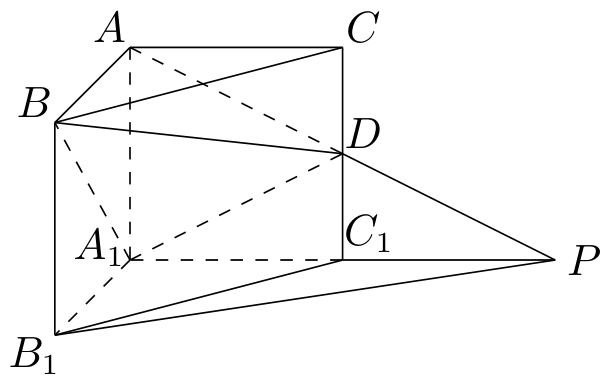
\includegraphics[width=6.3cm]{GaoKao/images/2011/sichuan_liberal/q19_fig1.png}
\end{center}

        \item 已知 \(\{a_n\}\) 是以 \(a\) 为首项，\(q\) 为公比的等比数列，\(S_n\) 为它的前 \(n\) 项和.
\begin{enumerate}
\item 当 \(S_1\)，\(S_3\)，\(S_4\) 成等差数列时，求 \(q\) 的值；
\item 当 \(S_m\)，\(S_n\)，\(S_l\) 成等差数列时，求证：对任意自然数 \(k\)，\(a_{m+k}\)，\(a_{n+k}\)，\(a_{l+k}\) 也成等差数列.
\end{enumerate}

        \item 过点 \(C(0, 1)\) 的椭圆 \(\frac{x^2}{a^2} + \frac{y^2}{b^2} = 1\)（\(a > b > 0\)） 的离心率为 \(\frac{\sqrt{3}}{2}\)，椭圆与 \(x\) 轴交于两点 \(A(a, 0)\)，\(B(-a, 0)\)，过点 \(C\) 的直线 \(l\) 与椭圆交于另一点 \(D\)，并与 \(x\) 轴交于点 \(P\)，直线 \(AC\) 与直线 \(BD\) 交于点 \(Q\).
\begin{enumerate}
\item 当直线 \(l\) 过椭圆右焦点时，求线段 \(CD\) 的长；
\item 当点 \(P\) 异于点 \(B\) 时，求证：\(\overrightarrow{OP} \cdot \overrightarrow{OQ}\) 为定值.
\end{enumerate}
\begin{center}
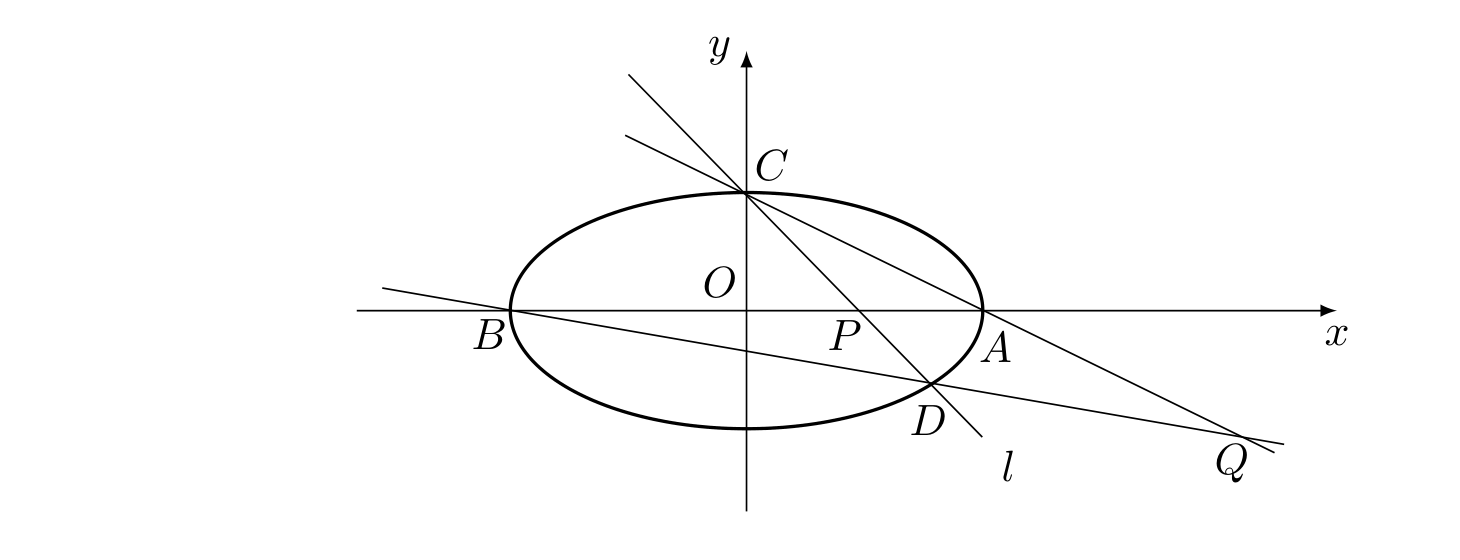
\includegraphics[width=0.90\linewidth]{GaoKao/images/2011/sichuan_liberal/q21_fig1.png}
\end{center}

        \item 已知函数 \(f(x) = \frac{2}{3}x + \frac{1}{2}\)，\(h(x) = \sqrt{x}\).
\begin{enumerate}
\item 设函数 \(F(x) = 18f(x) - x^2[h(x)]^2\)，求 \(F(x)\) 的单调区间与极值；
\item 设 \(a \in \mathbb{R}\)，解关于 \(x\) 的方程 \(\lg \left[ \frac{3}{2}f(x - 1) - \frac{3}{4} \right] = 2\lg h(a - x) - 2\lg h(4 - x)\)；
\item 设 \(n \in \mathbb{N}^{*}\)，证明：\(f(n)h(n) - [h(1) + h(2) + \cdots + h(n)] \geqslant \frac{1}{6}\).
\end{enumerate}

    \end{enumerate}

\end{description}


\subsection{2011年山东卷（理）}\label{gk:2011年山东卷（理）}

\begin{description}

    \item[一、选择题]

    \begin{enumerate}[leftmargin=5pt]

        \item 设集合 \(M = \{x \mid x^2 + x - 6 < 0\}\)，\(N = \{x \mid 1 \leqslant x \leqslant 3\}\). 则 \(M \cap N =\)（\quad）

        {\centering\begin{tabular*}{\linewidth}{@{}@{\extracolsep{\fill}}llll@{}}
          \text{A. }\([1, 2)\)  &  \text{B. }\([1, 2]\)  &  \text{C. }\((2, 3]\)  &  \text{D. }\([2, 3]\)
        \end{tabular*}\par}

        \item 复数 \(z = \frac{2 - \i}{2 + \i}\)（\(\i\) 为虚数单位）在复平面内对应的点所在的象限为（\quad）

        {\centering\begin{tabular*}{\linewidth}{@{}@{\extracolsep{\fill}}llll@{}}
          \text{A. }第一象限  &  \text{B. }第二象限  &  \text{C. }第三象限  &  \text{D. }第四象限
        \end{tabular*}\par}

        \item 若点 \((a,9)\) 在函数 \(y = 3^{x}\) 的图象上，则 \(\tan \frac{a\pi}{6}\) 的值为（\quad）

        {\centering\begin{tabular*}{\linewidth}{@{}@{\extracolsep{\fill}}llll@{}}
          \text{A. }0  &  \text{B. }\( \frac{\sqrt{3}}{3} \)  &  \text{C. }1  &  \text{D. }\(\sqrt{3}\)
        \end{tabular*}\par}

        \item 不等式 \( |x - 5| + |x + 3| \geqslant 10 \) 的解集是（\quad）

        {\centering\begin{tabular*}{\linewidth}{@{}@{\extracolsep{\fill}}llll@{}}
          \text{A. }\([-5,7]\)  &  \text{B. }\([-4,6]\)  &  \text{C. }\((- \infty, -5] \cup [7, +\infty)\)  &  \text{D. }\((- \infty, -4] \cup [6, +\infty)\)
        \end{tabular*}\par}

        \item 对于函数 \(y = f(x)\)，\(x \in \mathbb{R}\). “\( y = |f(x)| \) 的图象关于 \( y \) 轴对称”是“\( y = f(x) \) 是奇函数”的（\quad）

        {\centering\begin{tabular*}{\linewidth}{@{}@{\extracolsep{\fill}}llll@{}}
          \text{A. }充分而不必要条件  &  \text{B. }必要而不充分条件  &  \text{C. }充要条件  &  \text{D. }既不充分也不必要条件
        \end{tabular*}\par}

        \item 若函数 \( f(x) = \sin \omega x \)（\(\omega > 0\)）在区间 \(\left[0, \frac{\pi}{3}\right]\) 上单调递增，在区间 \(\left[\frac{\pi}{3}, \frac{\pi}{2}\right]\) 上单调递减，则 \(\omega =\)（\quad）

        {\centering\begin{tabular*}{\linewidth}{@{}@{\extracolsep{\fill}}llll@{}}
          \text{A. }3  &  \text{B. }2  &  \text{C. }\(\frac{3}{2}\)  &  \text{D. }\(\frac{2}{3}\)
        \end{tabular*}\par}

        \item 某产品的广告费用 \(x\) 与销售额 \(y\) 的统计数据如下表：

\begin{center}
\begin{tabular}{c|cccc}
广告费用 \(x\) （万元） & 4 & 2 & 3 & 5 \\
\hline
销售额 \(y\) （万元） & 49 & 26 & 39 & 54
\end{tabular}
\end{center}

根据上表可得回归方程 \( \hat{y} = \hat{b}x + \hat{a} \) 中的 \(\hat{b}\) 为 \(9.4\)，据此模型预报广告费用为 \(6\text{ 万元}\) 时销售额为（\quad）

        {\centering\begin{tabular*}{\linewidth}{@{}@{\extracolsep{\fill}}llll@{}}
          \text{A. }\(63.6\text{ 万元}\)  &  \text{B. }\(65.5\text{ 万元}\)  &  \text{C. }\(67.7\text{ 万元}\)  &  \text{D. }\(72.0\text{ 万元}\)
        \end{tabular*}\par}

        \item 已知双曲线 \(\frac{x^2}{a^2} - \frac{y^2}{b^2} = 1 \) （\(a > 0, b > 0\)）的两条渐近线均和圆 \(C: x^2 + y^2 - 6x + 5 = 0\) 相切，且双曲线右焦点为圆 \(C\) 的圆心，则该双曲线的方程为（\quad）

        {\centering\begin{tabular*}{\linewidth}{@{}@{\extracolsep{\fill}}llll@{}}
          \text{A. }\(\frac{x^2}{5} -\frac{y^2}{4} = 1\)  &  \text{B. }\(\frac{x^2}{4} -\frac{y^2}{5} = 1\)  &  \text{C. }\(\frac{x^2}{3} -\frac{y^2}{6} = 1\)  &  \text{D. }\(\frac{x^2}{6} -\frac{y^2}{3} = 1\)
        \end{tabular*}\par}

        \item 函数 \( y = \frac{x}{2} - 2\sin x \) 的图象大致是（\quad）

        {\centering\begin{tabular*}{\linewidth}{@{}@{\extracolsep{\fill}}cccc@{}}
          \text{A. }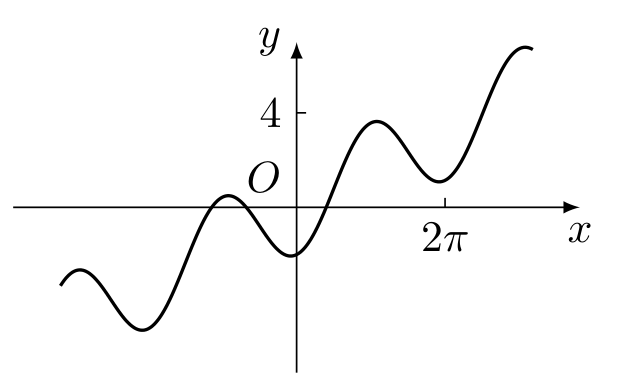
\includegraphics[width=0.15\paperwidth]{GaoKao/images/2011/shandong_science/q9_choice_a.png}  &  \text{B. }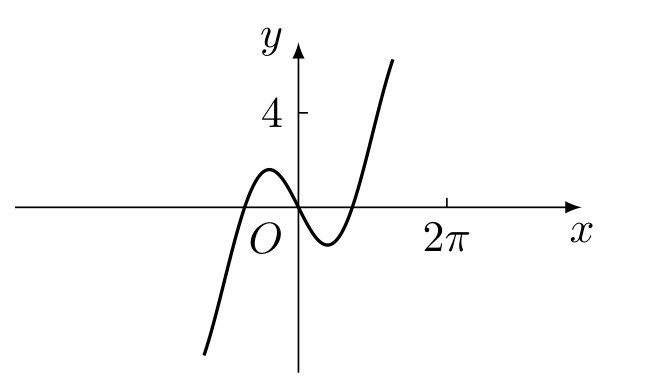
\includegraphics[width=0.15\paperwidth]{GaoKao/images/2011/shandong_science/q9_choice_b.png}  &  \text{C. }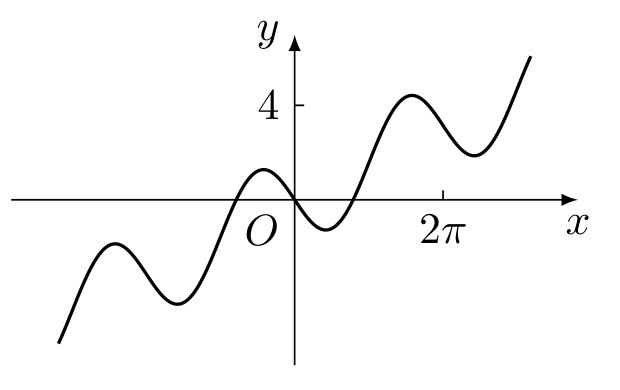
\includegraphics[width=0.15\paperwidth]{GaoKao/images/2011/shandong_science/q9_choice_c.png}  &  \text{D. }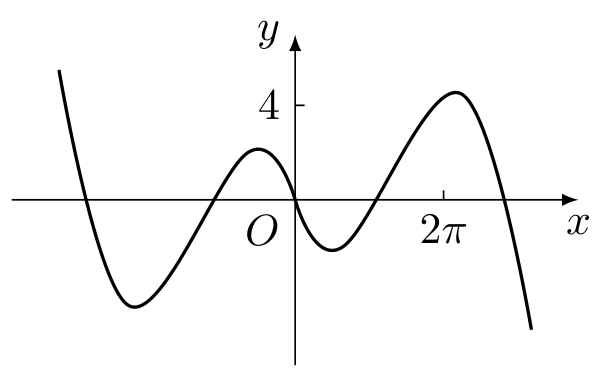
\includegraphics[width=0.15\paperwidth]{GaoKao/images/2011/shandong_science/q9_choice_d.png}
        \end{tabular*}\par}

        \item 已知 \( f(x) \) 是 \( \mathbb{R} \) 上最小正周期为 2 的周期函数，且当 \( 0 \leqslant x < 2 \) 时，\( f(x) = x^3 - x \)，则函数 \( y = f(x) \) 的图象在区间 \([0, 6]\) 上与 \( x \) 轴的交点的个数为（\quad）

        {\centering\begin{tabular*}{\linewidth}{@{}@{\extracolsep{\fill}}llll@{}}
          \text{A. }6  &  \text{B. }7  &  \text{C. }8  &  \text{D. }9
        \end{tabular*}\par}

        \item 如图是长和宽分别相等的两个矩形. 给定下列三个命题：

\begin{enumerate}
\item 存在三棱柱，其正（主）视图，俯视图如图；
\item 存在四棱柱，其正（主）视图，俯视图如图；
\item 存在圆柱，其正（主）视图，俯视图如图.
\end{enumerate}

其中真命题的个数是（\quad）
\begin{center}
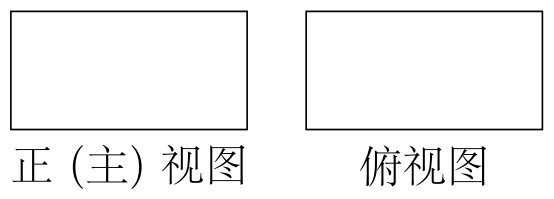
\includegraphics[width=5.6cm]{GaoKao/images/2011/shandong_science/q11_fig1.png}
\end{center}

        {\centering\begin{tabular*}{\linewidth}{@{}@{\extracolsep{\fill}}llll@{}}
          \text{A. }3  &  \text{B. }2  &  \text{C. }1  &  \text{D. }0
        \end{tabular*}\par}

        \item 设 \(A_{1}\)，\(A_{2}\)，\(A_{3}\)，\(A_{4}\) 是平面直角坐标系中两两不同的四点. 若 \(\overrightarrow{A_{1}A_{3}} = \lambda \overrightarrow{A_{1}A_{2}}\) （\(\lambda \in \mathbb{R}\)），\(\overrightarrow{A_{1}A_{4}} = \mu \overrightarrow{A_{1}A_{2}}\) （\(\mu \in \mathbb{R}\)），且 \(\frac{1}{\lambda} + \frac{1}{\mu} = 2\)，则称 \(A_{3}\)，\(A_{4}\) 调和分割 \(A_{1}\)，\(A_{2}\). 已知平面上的点 \(C\)，\(D\) 调和分割点 \(A\)，\(B\)，则下面说法正确的是（\quad）

        {\centering\begin{tabular*}{\linewidth}{@{}@{\extracolsep{\fill}}llll@{}}
          \text{A. }\(C\) 可能是线段 \(AB\) 的中点  &  \text{B. }\(D\) 可能是线段 \(AB\) 的中点  &  \text{C. }\(C\)，\(D\) 可能同时在线段 \(AB\) 上  &  \text{D. }\(C\)，\(D\) 不可能同时在线段 \(AB\) 的延长线上
        \end{tabular*}\par}

    \end{enumerate}

\end{description}

\begin{description}

    \item[二、填空题]

    \begin{enumerate}[leftmargin=5pt]

      \addtocounter{enumi}{+12}

        \item 执行如图所示的程序框图，输入 \(l = 2\)，\(m = 3\)，\(n = 5\)，则输出的 \(y\) 的值是\rule[-0.3ex]{3em}{0.4pt}.

\begin{center}
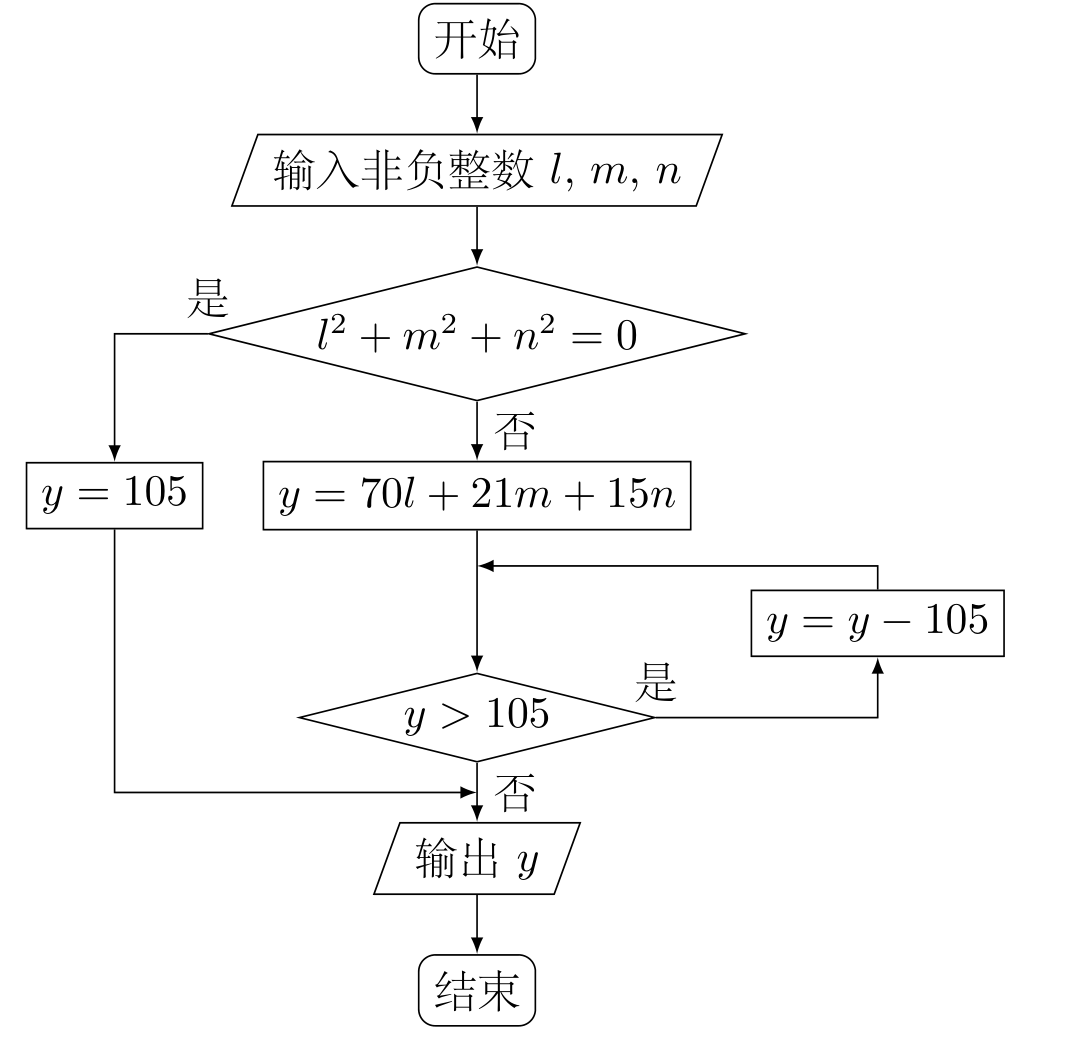
\includegraphics[width=6.5cm]{GaoKao/images/2011/shandong_science/q13_fig1.png}
\end{center}

        \item 若 \(\left(x - \frac{\sqrt{a}}{x^{2}}\right)^6\) 展开式的常数项为 60，则常数 \(a\) 的值为\rule[-0.3ex]{3em}{0.4pt}.

        \item 设函数 \(f(x) = \frac{x}{x + 2}\)（\(x > 0\)），观察：\(f_{1}(x) = f(x) = \frac{x}{x + 2}\)，\(f_{2}(x) = f\!\left(f_{1}(x)\right) = \frac{x}{3x + 4}\)，\(f_{3}(x) = f\!\left(f_{2}(x)\right) = \frac{x}{7x + 8}\)，\(f_{4}(x) = f\!\left(f_{3}(x)\right) = \frac{x}{15x + 16}\). 根据以上事实，由归纳推理可得：当 \(n \in \mathbb{N}^{*}\) 且 \(n \geqslant 2\) 时，\(f_n(x) = f(f_{n-1}(x)) =\)\rule[-0.3ex]{3em}{0.4pt}.

        \item 已知函数 \( f(x) = \log_a x + x - b \)（\(a > 0\)，且 \(a \neq 1\)）. 当 \( 2 < a < 3 < b < 4 \) 时，函数 \( f(x) \) 的零点 \(x_0 \in (n, n+1)\)，\(n \in \mathbb{N}^{*}\)，则 \( n = \)\rule[-0.3ex]{3em}{0.4pt}.

    \end{enumerate}

\end{description}

\begin{description}

    \item[三、解答题]

    \begin{enumerate}[leftmargin=5pt]

      \addtocounter{enumi}{+16}

        \item 在 \(\triangle ABC\) 中，内角 \(A\)，\(B\)，\(C\) 的对边分别为 \(a\)，\(b\)，\(c\)，已知 \(\frac{\cos A - 2 \cos C}{\cos B} = \frac{2c - a}{b}\).
\begin{enumerate}
\item 求 \(\frac{\sin C}{\sin A}\) 的值；
\item 若 \(\cos B = \frac{1}{4}\)，\(b = 2\)，求 \(\triangle ABC\) 的面积 \(S\).
\end{enumerate}

        \item 红队队员甲，乙，丙与蓝队队员 \(A\)，\(B\)，\(C\) 进行围棋比赛，甲对 \(A\)，乙对 \(B\)，丙对 \(C\) 各一盘. 已知甲胜 \(A\)，乙胜 \(B\)，丙胜 \(C\) 的概率分别为 \(0.6\)，\(0.5\)，\(0.5\). 假设各盘比赛结果相互独立.
\begin{enumerate}
\item 求红队至少两名队员获胜的概率；
\item 用 \(\xi\) 表示红队队员获胜的总数，求 \(\xi\) 的分布列和数学期望 \(E(\xi)\).
\end{enumerate}

        \item 在如图所示的几何体中，四边形 \(ABCD\) 为平行四边形，\(\angle ACB = 90^{\circ}\)，\(EA \perp\) 平面 \(ABCD\)，\(EF \parallel AB\)，\(FG \parallel BC\)，\(EG \parallel AC\)，\(AB = 2EF\).
\begin{enumerate}
\item 若 \(M\) 是线段 \(AD\) 的中点，求证：\(GM \parallel\) 平面 \(ABFE\)；
\item 若 \(AC = BC = 2AE\)，求二面角 \(A - BF - C\) 的大小.
\end{enumerate}

\begin{center}
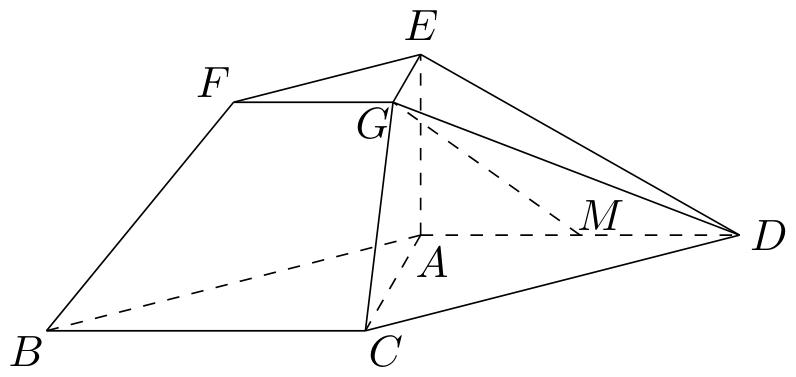
\includegraphics[width=9.9cm]{GaoKao/images/2011/shandong_science/q19_fig1.png}
\end{center}

        \item 等比数列 \(\{a_{n}\}\) 中，\(a_{1}\)，\(a_{2}\)，\(a_{3}\) 分别是下表第一，二，三行中的某一个数，且 \(a_{1}\)，\(a_{2}\)，\(a_{3}\) 中的任何两个数不在下表的同一列.

\begin{center}
\begin{tabular}{c|ccc}
 & 第一列 & 第二列 & 第三列 \\
\hline
第一行 & 3 & 2 & 10 \\
第二行 & 6 & 4 & 14 \\
第三行 & 9 & 8 & 18
\end{tabular}
\end{center}

\begin{enumerate}
\item 求数列 \(\{a_{n}\}\) 的通项公式；
\item 若数列 \(\{b_{n}\}\) 满足： \(b_{n} = a_{n} + (-1)^{n} \ln a_{n}\)，求数列 \(\{b_{n}\}\) 的前 \(n\) 项和 \(S_{n}\).
\end{enumerate}

        \item 某企业拟建造如图所示的容器（不计厚度，长度单位：米），其中容器的中间为圆柱形，左右两端均为半球形，按照设计要求容器的容积为 \(\frac{80\pi}{3}\text{ 立方米}\)，且 \(l\geqslant2r\). 假设该容器的建造费用仅与其表面积有关. 已知圆柱形部分每平方米建造费用为 \(3\text{ 千元}\)，半球形部分每平方米建造费用为 \(c\text{ 千元}\)（\(c>3\)）. 设该容器的建造费用为 \(y\text{ 千元}\).
\begin{enumerate}
\item 写出 \(y\) 关于 \(r\) 的函数表达式，并求该函数的定义域；
\item 求该容器的建造费用最小时的 \(r\).
\end{enumerate}

\begin{center}
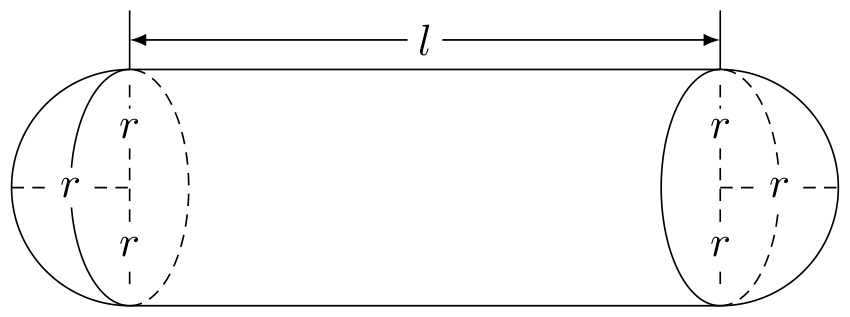
\includegraphics[width=15.5cm]{GaoKao/images/2011/shandong_science/q21_fig1.png}
\end{center}

        \item 已知动直线 \(l\) 与椭圆 \(C: \frac{x^2}{3} + \frac{y^2}{2} = 1\) 交于 \(P(x_1, y_1)\)，\(Q(x_2, y_2)\) 两不同点，且 \(\triangle OPQ\) 的面积 \(S_{\triangle OPQ} = \frac{\sqrt{6}}{2}\). 其中 \(O\) 为坐标原点.
\begin{enumerate}
\item 证明： \(x_1^2 + x_2^2\) 和 \(y_1^2 + y_2^2\) 均为定值；
\item 设线段 \(PQ\) 的中点为 \(M\)，求 \(|OM| \cdot |PQ|\) 的最大值；
\item 椭圆 \(C\) 上是否存在三点 \(D\)，\(E\)，\(G\)，使得 \(S_{\triangle DOE} = S_{\triangle ODG} = S_{\triangle OEG} = \frac{\sqrt{6}}{2}\)；若存在，判断 \(\triangle DEG\) 的形状；若不存在，请说明理由.
\end{enumerate}

    \end{enumerate}

\end{description}


\subsection{2011年山东卷（文）}\label{gk:2011年山东卷（文）}

\begin{description}

    \item[一、选择题]

    \begin{enumerate}[leftmargin=5pt]

        \item 设集合 \(M = \{x \mid (x + 3)(x - 2) < 0\}\)，\(N = \{x \mid 1 \leqslant x \leqslant 3\}\)，则 \(M \cap N =\)（\quad）

        {\centering\begin{tabular*}{\linewidth}{@{}@{\extracolsep{\fill}}llll@{}}
          \text{A. }\([1,2)\)  &  \text{B. }\([1,2]\)  &  \text{C. }\((2,3]\)  &  \text{D. }\([2,3]\)
        \end{tabular*}\par}

        \item 复数 \(z = \frac{2 - \i}{2 + \i}\)（\(\i\) 为虚数单位）在复平面内对应的点所在的象限为（\quad）

        {\centering\begin{tabular*}{\linewidth}{@{}@{\extracolsep{\fill}}llll@{}}
          \text{A. }第一象限  &  \text{B. }第二象限  &  \text{C. }第三象限  &  \text{D. }第四象限
        \end{tabular*}\par}

        \item 若点 \((a,9)\) 在函数 \(y = 3^{x}\) 的图象上，则 \(\tan \frac{a\pi}{6}\) 的值为（\quad）

        {\centering\begin{tabular*}{\linewidth}{@{}@{\extracolsep{\fill}}llll@{}}
          \text{A. }0  &  \text{B. }\(\frac{\sqrt{3}}{3}\)  &  \text{C. }1  &  \text{D. }\(\sqrt{3}\)
        \end{tabular*}\par}

        \item 曲线 \( y = x^{3} + 11 \) 在点 \( P(1,12) \) 处的切线与 \( y \) 轴交点的纵坐标是（\quad）

        {\centering\begin{tabular*}{\linewidth}{@{}@{\extracolsep{\fill}}llll@{}}
          \text{A. }\(-9\)  &  \text{B. }\(-3\)  &  \text{C. }9  &  \text{D. }15
        \end{tabular*}\par}

        \item 已知 \(a\)，\(b\)，\(c \in \mathbb{R}\)，命题“若 \(a + b + c = 3\)，则 \(a^2 + b^2 + c^2 \geqslant 3\)”的否命题是（\quad）

        {\centering\begin{tabular*}{\linewidth}{@{}@{\extracolsep{\fill}}llll@{}}
          \text{A. }若 \(a + b + c \neq 3\)，则 \(a^2 + b^2 + c^2 < 3\)  &  \text{B. }若 \(a + b + c = 3\)，则 \(a^2 + b^2 + c^2 < 3\)  &  \text{C. }若 \(a + b + c \neq 3\)，则 \(a^2 + b^2 + c^2 \geqslant 3\)  &  \text{D. }若 \(a^2 + b^2 + c^2 \geqslant 3\)，则 \(a + b + c = 3\)
        \end{tabular*}\par}

        \item 若函数 \(f(x) = \sin \omega x\)（\(\omega > 0\)） 在区间 \(\left[0, \frac{\pi}{3}\right]\) 上单调递增，在区间 \(\left[\frac{\pi}{3}, \frac{\pi}{2}\right]\) 上单调递减，则 \(\omega =\)（\quad）

        {\centering\begin{tabular*}{\linewidth}{@{}@{\extracolsep{\fill}}llll@{}}
          \text{A. }\(\frac{2}{3}\)  &  \text{B. }\(\frac{3}{2}\)  &  \text{C. }2  &  \text{D. }3
        \end{tabular*}\par}

        \item 设变量 \(x\)，\(y\) 满足约束条件 \(\begin{cases}
x + 2y - 5 \leqslant 0,\\
x - y - 2 \leqslant 0,\\
x \geqslant 0,
\end{cases}\) 则目标函数 \(z = 2x + 3y + 1\) 的最大值为（\quad）

        {\centering\begin{tabular*}{\linewidth}{@{}@{\extracolsep{\fill}}llll@{}}
          \text{A. }11  &  \text{B. }10  &  \text{C. }9  &  \text{D. }8.5
        \end{tabular*}\par}

        \item 某产品的广告费用 \(x\) 与销售额 \(y\) 的统计数据如下表：

\begin{center}
\begin{tabular}{c|cccc}
广告费用 \(x\)（万元） & 4 & 2 & 3 & 5 \\
\hline
销售额 \(y\)（万元） & 49 & 26 & 39 & 54
\end{tabular}
\end{center}

根据上表可得回归方程 \(\hat{y} = \hat{b}x + \hat{a}\) 中的 \(\hat{b}\) 为 9.4，据此模型预报广告费用为 6 万元时销售额为（\quad）

        {\centering\begin{tabular*}{\linewidth}{@{}@{\extracolsep{\fill}}llll@{}}
          \text{A. }\(63.6\text{ 万元}\)  &  \text{B. }\(65.5\text{ 万元}\)  &  \text{C. }\(67.7\text{ 万元}\)  &  \text{D. }\(72.0\text{ 万元}\)
        \end{tabular*}\par}

        \item 设 \(M(x_0, y_0)\) 为抛物线 \(C: x^2 = 8y\) 上一点，\(F\) 为抛物线 \(C\) 的焦点，以 \(F\) 为圆心，\(|FM|\) 为半径的圆和抛物线 \(C\) 的准线相交，则 \(y_0\) 的取值范围是（\quad）

        {\centering\begin{tabular*}{\linewidth}{@{}@{\extracolsep{\fill}}llll@{}}
          \text{A. }\((0,2)\)  &  \text{B. }\([0,2]\)  &  \text{C. }\((2, + \infty)\)  &  \text{D. }\([2, + \infty)\)
        \end{tabular*}\par}

        \item 函数 \( y = \frac{x}{2} - 2\sin x \) 的图象大致是（\quad）

        {\centering\begin{tabular*}{\linewidth}{@{}@{\extracolsep{\fill}}cccc@{}}
          \text{A. }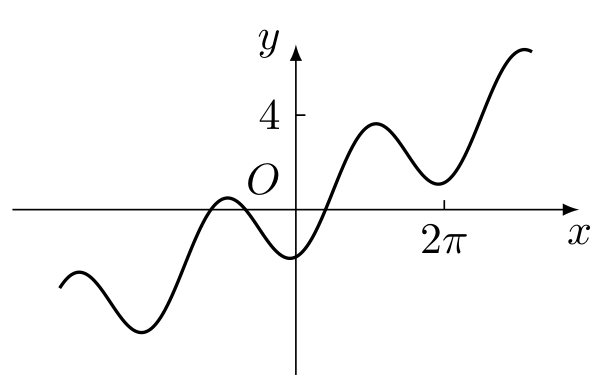
\includegraphics[width=0.15\paperwidth]{GaoKao/images/2011/shandong_liberal/q10_choice_a.png}  &  \text{B. }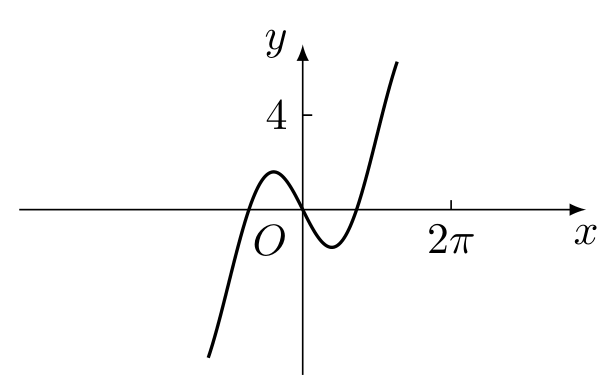
\includegraphics[width=0.15\paperwidth]{GaoKao/images/2011/shandong_liberal/q10_choice_b.png}  &  \text{C. }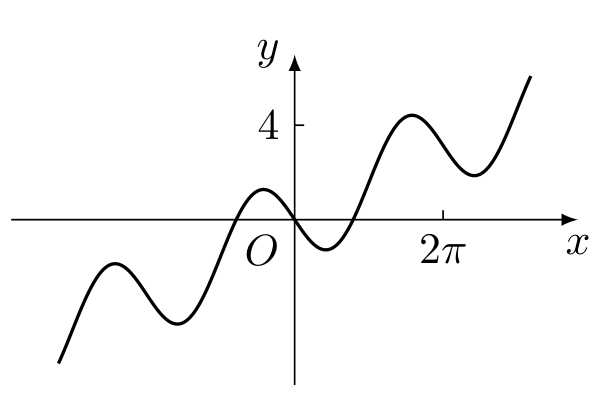
\includegraphics[width=0.15\paperwidth]{GaoKao/images/2011/shandong_liberal/q10_choice_c.png}  &  \text{D. }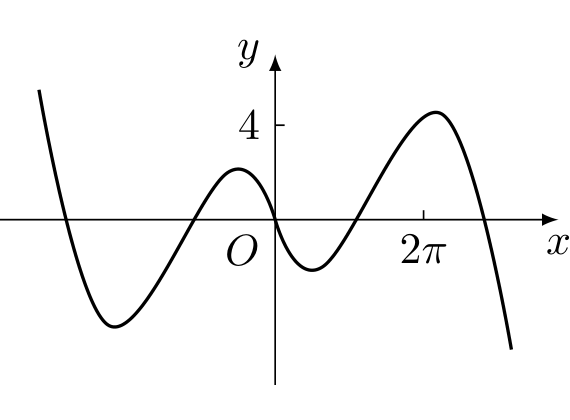
\includegraphics[width=0.15\paperwidth]{GaoKao/images/2011/shandong_liberal/q10_choice_d.png}
        \end{tabular*}\par}

        \item 如图是长和宽分别相等的两个矩形. 给定下列三个命题：
\begin{enumerate}
\item 存在三棱柱，其正（主）视图，俯视图如图；
\item 存在四棱柱，其正（主）视图，俯视图如图；
\item 存在圆柱，其正（主）视图，俯视图如图.
\end{enumerate}
其中真命题的个数是（\quad）

\begin{center}
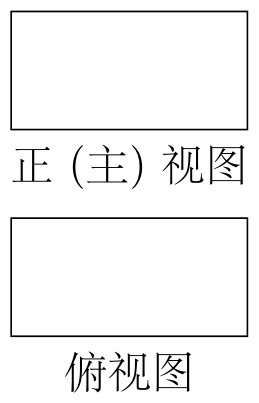
\includegraphics[width=2.5cm]{GaoKao/images/2011/shandong_liberal/q11_fig1.png}
\end{center}

        {\centering\begin{tabular*}{\linewidth}{@{}@{\extracolsep{\fill}}llll@{}}
          \text{A. }3  &  \text{B. }2  &  \text{C. }1  &  \text{D. }0
        \end{tabular*}\par}

        \item 设 \(A_{1}\)，\(A_{2}\)，\(A_{3}\)，\(A_{4}\) 是平面直角坐标系中两两不同的四点，若 \(\overrightarrow{A_{1}A_{3}} = \lambda \overrightarrow{A_{1}A_{2}}\) （\(\lambda \in \mathbb{R}\)），\(\overrightarrow{A_{1}A_{4}} = \mu \overrightarrow{A_{1}A_{2}}\) （\(\mu \in \mathbb{R}\)），且 \(\frac{1}{\lambda} + \frac{1}{\mu} = 2\)，则称 \(A_{3}\)，\(A_{4}\) 调和分割 \(A_{1}\)，\(A_{2}\). 已知点 \(C(c, 0)\)，\(D(d, 0)\) （\(c\)，\(d \in \mathbb{R}\)） 调和分割点 \(A(0, 0)\)，\(B(1, 0)\)，则下面说法正确的是（\quad）

        {\centering\begin{tabular*}{\linewidth}{@{}@{\extracolsep{\fill}}llll@{}}
          \text{A. }\(C\) 可能是线段 \(AB\) 的中点  &  \text{B. }\(D\) 可能是线段 \(AB\) 的中点  &  \text{C. }\(C\)，\(D\) 可能同时在线段 \(AB\) 上  &  \text{D. }\(C\)，\(D\) 不可能同时在线段 \(AB\) 的延长线上
        \end{tabular*}\par}

    \end{enumerate}

\end{description}

\begin{description}

    \item[二、填空题]

    \begin{enumerate}[leftmargin=5pt]

      \addtocounter{enumi}{+12}

        \item 某高校甲，乙，丙，丁四个专业分别有 150，150，400，300 名学生，为了解学生的就业倾向，用分层抽样的方法从该校这四个专业共抽取 40 名学生进行调查，应在丙专业抽取的学生人数为\rule[-0.3ex]{3em}{0.4pt}.

        \item 执行如图所示的程序框图，输入 \(l = 2\)，\(m = 3\)，\(n = 5\)，则输出的 \(y\) 的值是\rule[-0.3ex]{3em}{0.4pt}.

\begin{center}
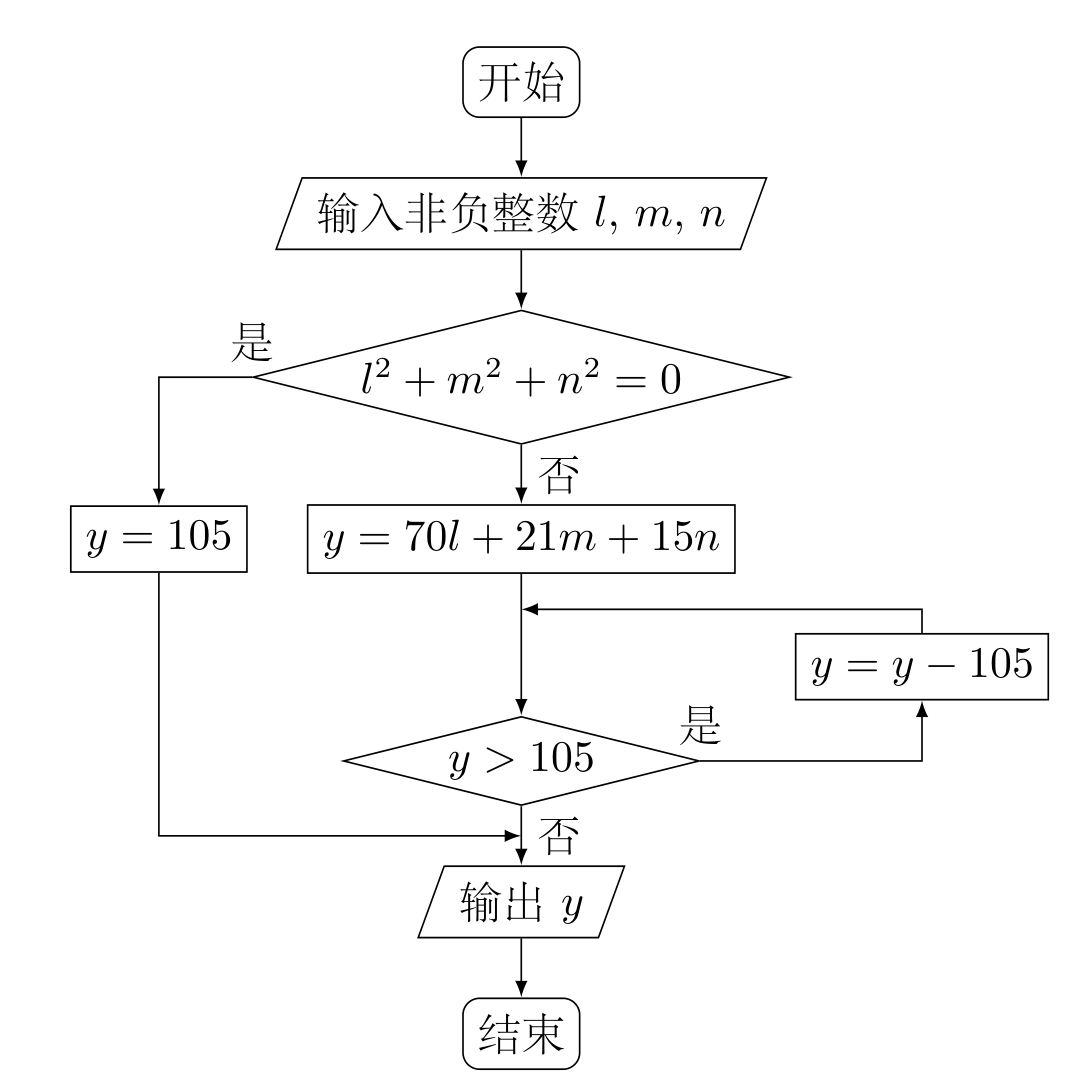
\includegraphics[width=6.8cm]{GaoKao/images/2011/shandong_liberal/q14_fig1.png}
\end{center}

        \item 已知双曲线 \(\frac{x^2}{a^2} - \frac{y^2}{b^2} = 1\)（\(a > 0\)，\(b > 0\)）和椭圆 \(\frac{x^2}{16} + \frac{y^2}{9} = 1\) 有相同的焦点，且双曲线的离心率是椭圆离心率的两倍，则双曲线的方程为\rule[-0.3ex]{3em}{0.4pt}.

        \item 已知函数 \(f(x) = \log_a x + x - b\)（\(a > 0\)，且 \(a \neq 1\)）. 当 \(2 < a < 3 < b < 4\) 时，函数 \(f(x)\) 的零点 \(x_0 \in (n, n + 1)\)，\(n \in \mathbb{N}^*\)，则 \(n = \)\rule[-0.3ex]{3em}{0.4pt}.

    \end{enumerate}

\end{description}

\begin{description}

    \item[三、解答题]

    \begin{enumerate}[leftmargin=5pt]

      \addtocounter{enumi}{+16}

        \item 在 \(\triangle ABC\) 中，内角 \(A\)，\(B\)，\(C\) 的对边分别为 \(a\)，\(b\)，\(c\)，已知 \(\frac{\cos A - 2\cos C}{\cos B} = \frac{2c - a}{b}\).
\begin{enumerate}
\item 求 \( \frac{\sin C}{\sin A} \) 的值；
\item 若 \( \cos B = \frac{1}{4} \)，\( \triangle ABC \) 的周长为 5，求 \(b\) 的长.
\end{enumerate}

        \item 甲，乙两校各有 3 名教师报名支教. 其中甲校 2 男 1 女，乙校 1 男 2 女.
\begin{enumerate}
\item 若从甲校和乙校报名的教师中各任选 1 名，写出所有可能的结果，并求选出的 2 名教师性别相同的概率；
\item 若从报名的 6 名教师中任选 2 名，写出所有可能的结果，并求选出的 2 名教师来自同一学校的概率.
\end{enumerate}

        \item 如图，在四棱台 \(ABCD - A_{1}B_{1}C_{1}D_{1}\) 中，\(D_{1}D \perp\) 平面 \(ABCD\)，底面 \(ABCD\) 是平行四边形，\(AB = 2AD\)，\(AD = A_{1}B_{1}\)，\(\angle BAD = 60^{\circ}\).
\begin{enumerate}
\item 证明： \(AA_{1} \perp BD\).
\item 证明：\(CC_{1} \parallel\) 平面 \(A_{1}BD\).
\end{enumerate}

\begin{center}
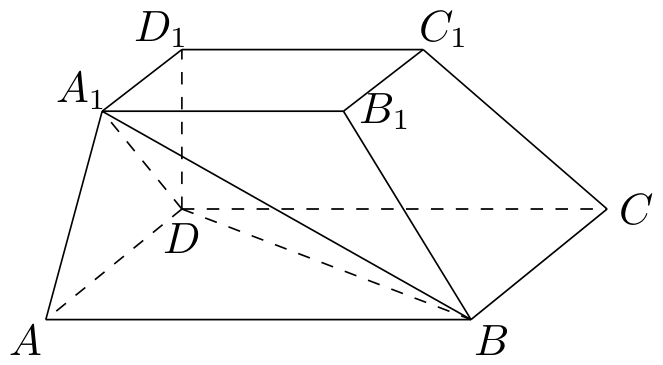
\includegraphics[width=6.8cm]{GaoKao/images/2011/shandong_liberal/q19_fig1.png}
\end{center}

        \item 等比数列 \(\{a_{n}\}\) 中，\(a_{1}\)，\(a_{2}\)，\(a_{3}\) 分别是下表第一、二、三行中的某一个数，且 \(a_{1}\)，\(a_{2}\)，\(a_{3}\) 中的任何两个数不在下表的同一列.

\begin{center}
\begin{tabular}{c|ccc}
 & 第一列 & 第二列 & 第三列 \\
\hline
第一行 & 3 & 2 & 10 \\
第二行 & 6 & 4 & 14 \\
第三行 & 9 & 8 & 18
\end{tabular}
\end{center}

\begin{enumerate}
\item 求数列 \(\{a_{n}\}\) 的通项公式；
\item 若数列 \(\{b_{n}\}\) 满足：\(b_{n}=a_{n}+(-1)^{n}\ln a_{n}\)，求数列 \(\{b_{n}\}\) 的前 \(2n\) 项和 \(S_{2n}\).
\end{enumerate}

        \item 某企业拟建造如图所示的容器（不计厚度，长度单位：米），其中容器的中间为圆柱形，左右两端均为半球形，按照设计要求容器的容积为 \(\frac{80\pi}{3}\) 立方米，且 \(l \geqslant 2r\). 假设该容器的建造费用仅与其表面积有关. 已知圆柱形部分每平方米建造费用为 3 千元，半球形部分每平方米建造费用为 \(c \) （\(c > 3\)）千元. 设该容器的建造费用为 \(y\) 千元.
\begin{enumerate}
\item 写出 \(y\) 关于 \(r\) 的函数表达式，并求该函数的定义域；
\item 求该容器的建造费用最小时的 \(r\).
\end{enumerate}

\begin{center}
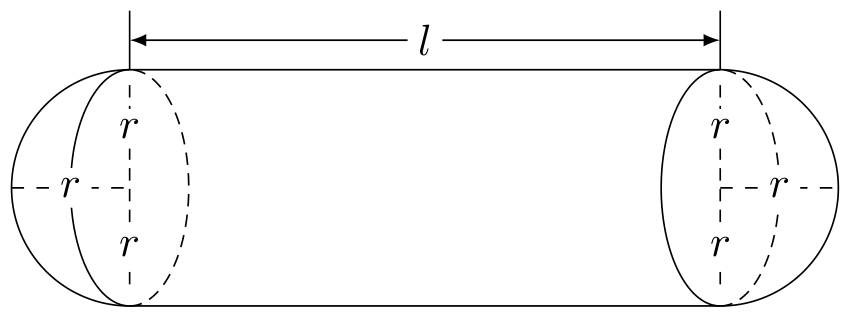
\includegraphics[width=14.2cm]{GaoKao/images/2011/shandong_liberal/q21_fig1.png}
\end{center}

        \item 在平面直角坐标系 \(xOy\) 中，已知椭圆 \(C: \frac{x^2}{3} + y^2 = 1\). 如图所示，斜率为 \(k \) （\(k > 0\)）且不过原点的直线 \(l\) 交椭圆 \(C\) 于 \(A\)，\(B\) 两点. 线段 \(AB\) 的中点为 \(E\). 射线 \(OE\) 交椭圆 \(C\) 于点 \(G\)，交直线 \(x = -3\) 于点 \(D(-3, m)\).
\begin{enumerate}
\item 求 \(m^{2} + k^{2}\) 的最小值；
\item 若 \(\left|OG\right|^{2}=\left|OD\right|\cdot\left|OE\right|\)，
\begin{enumerate}
\item 求证：直线 \(l\) 过定点；
\item 试问点 \(B\)，\(G\) 能否关于 \(x\) 轴对称？若能，求出此时 \(\triangle ABG\) 的外接圆方程. 若不能，请说明理由.
\end{enumerate}
\end{enumerate}

\begin{center}
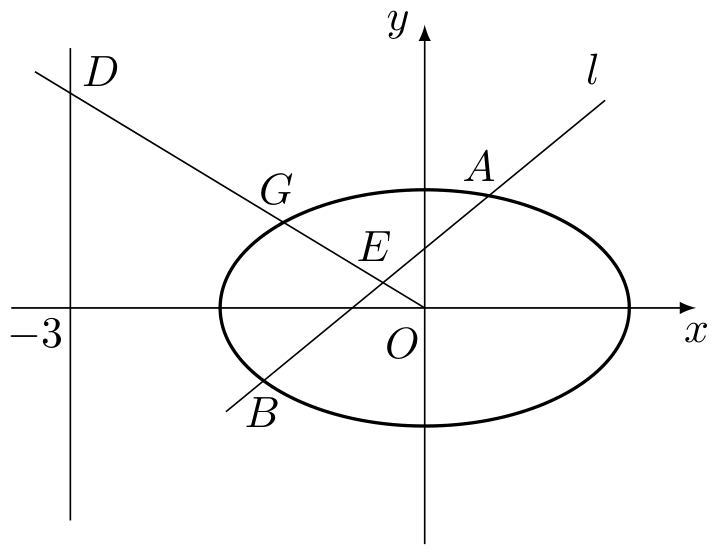
\includegraphics[width=9.5cm]{GaoKao/images/2011/shandong_liberal/q22_fig1.png}
\end{center}

    \end{enumerate}

\end{description}


\subsection{2011年陕西卷（理）}\label{gk:2011年陕西卷（理）}

\begin{description}

    \item[一、选择题]

    \begin{enumerate}[leftmargin=5pt]

        \item 设 \(\bm{a}\)，\(\bm{b}\) 是向量，命题“若 \(\bm{a} = -\bm{b}\)，则 \(|\bm{a}| = |\bm{b}|\)”的逆命题是（\quad）

        {\centering\begin{tabular*}{\linewidth}{@{}@{\extracolsep{\fill}}llll@{}}
          \text{A. }若 \(\bm{a} \neq -\bm{b}\)，则 \(|\bm{a}| \neq |\bm{b}|\).  &  \text{B. }若 \(\bm{a} = -\bm{b}\)，则 \(|\bm{a}| \neq |\bm{b}|\)  &  \text{C. }若 \(|\bm{a}| \neq |\bm{b}|\)，则 \(\bm{a} \neq -\bm{b}\)  &  \text{D. }若 \(|\bm{a}| = |\bm{b}|\)，则 \(\bm{a} = -\bm{b}\)
        \end{tabular*}\par}

        \item 设抛物线的顶点在原点，准线方程为 \(x = -2\)，则抛物线的方程是（\quad）

        {\centering\begin{tabular*}{\linewidth}{@{}@{\extracolsep{\fill}}llll@{}}
          \text{A. }\( y^{2} = -8x \)  &  \text{B. }\( y^{2} = -4x \)  &  \text{C. }\( y^{2} = 8x \)  &  \text{D. }\( y^{2} = 4x \)
        \end{tabular*}\par}

        \item 设函数 \( f(x) \) （\(x \in \mathbb{R}\)）满足 \(f(-x) = f(x)\)，\(f(x + 2) = f(x)\)，则 \( y = f(x) \) 的图象可能是（\quad）

        {\centering\begin{tabular*}{\linewidth}{@{}@{\extracolsep{\fill}}cccc@{}}
          \text{A. }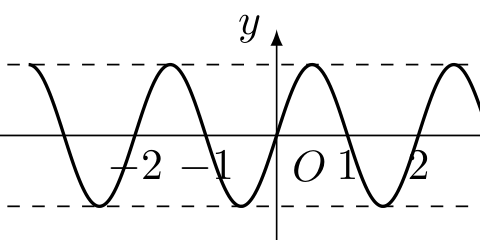
\includegraphics[width=0.15\paperwidth]{GaoKao/images/2011/shaanxi_science/q3_optA_clean.png}  &  \text{B. }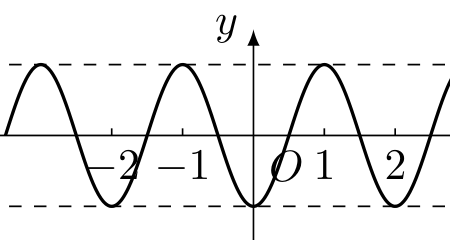
\includegraphics[width=0.15\paperwidth]{GaoKao/images/2011/shaanxi_science/q3_optB_clean.png}  &  \text{C. }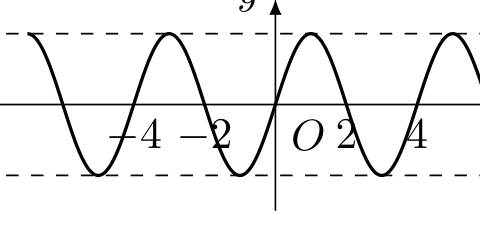
\includegraphics[width=0.15\paperwidth]{GaoKao/images/2011/shaanxi_science/q3_optC_clean.png}  &  \text{D. }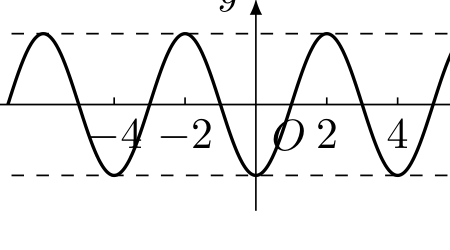
\includegraphics[width=0.15\paperwidth]{GaoKao/images/2011/shaanxi_science/q3_optD_clean.png}
        \end{tabular*}\par}

        \item \((4^{x} - 2^{-x})^{6}\)（\(x \in \mathbb{R}\)）展开式中的常数项是（\quad）

        {\centering\begin{tabular*}{\linewidth}{@{}@{\extracolsep{\fill}}llll@{}}
          \text{A. }\(-20\)  &  \text{B. }\(-15\)  &  \text{C. }15  &  \text{D. }20
        \end{tabular*}\par}

        \item 某几何体的三视图如图所示，则它的体积是（\quad）

\begin{center}
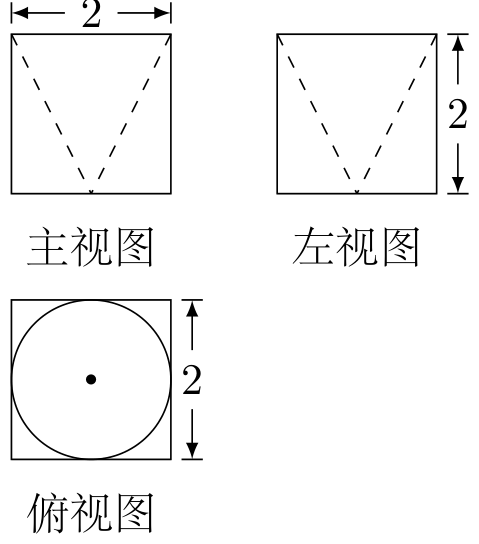
\includegraphics[width=4.7cm]{GaoKao/images/2011/shaanxi_science/q5_fig1.png}
\end{center}

        {\centering\begin{tabular*}{\linewidth}{@{}@{\extracolsep{\fill}}llll@{}}
          \text{A. }\(8 - \frac{2\pi}{3}\)  &  \text{B. }\(8 - \frac{\pi}{3}\)  &  \text{C. }\(8 - 2\pi\)  &  \text{D. }\(\frac{2\pi}{3}\)
        \end{tabular*}\par}

        \item 函数 \( f(x) = \sqrt{x} - \cos x \) 在 \([0, +\infty)\) 内（\quad）

        {\centering\begin{tabular*}{\linewidth}{@{}@{\extracolsep{\fill}}llll@{}}
          \text{A. }没有零点  &  \text{B. }有且仅有一个零点  &  \text{C. }有且仅有两个零点  &  \text{D. }有无穷多个零点
        \end{tabular*}\par}

        \item 设集合 \(M = \{y \mid y = |\cos^2 x - \sin^2 x|, x \in \mathbb{R}\}\)，\(N = \left\{x \mid \left|x - \frac{1}{\i}\right| < \sqrt{2}, x \in \mathbb{R}\right\}\)，其中 \(\i\) 为虚数单位，则 \(M \cap N\) 为（\quad）

        {\centering\begin{tabular*}{\linewidth}{@{}@{\extracolsep{\fill}}llll@{}}
          \text{A. }\((0,1)\)  &  \text{B. }\((0,1]\)  &  \text{C. }\([0,1)\)  &  \text{D. }\([0,1]\)
        \end{tabular*}\par}

        \item 如图，\(x_{1}\)，\(x_{2}\)，\(x_{3}\) 为某次考试三个评阅人对同一道题的独立评分，\(p\) 为该题的最终得分，当 \(x_{1} = 6\)，\(x_{2} = 9\)，\(p = 8.5\) 时，\(x_{3}\) 等于（\quad）

\begin{center}
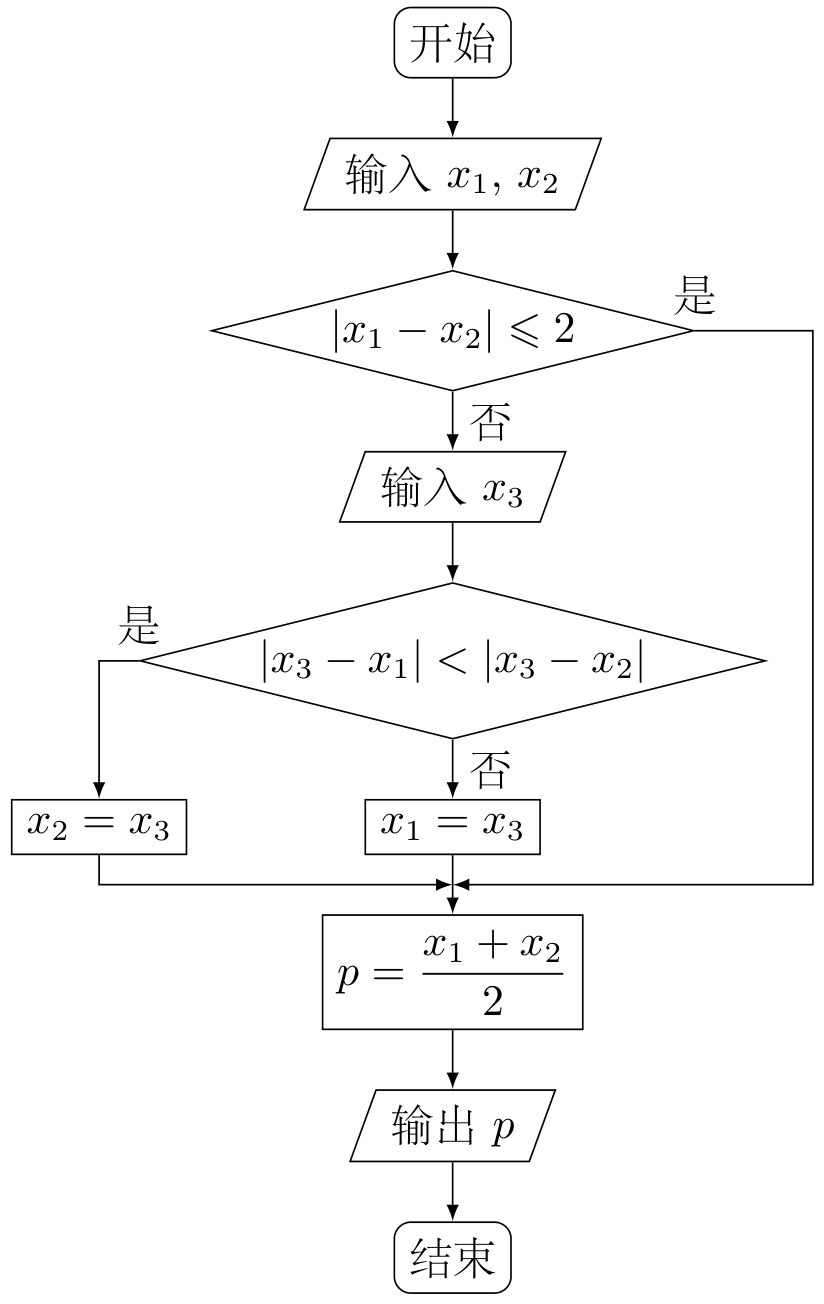
\includegraphics[width=4.7cm]{GaoKao/images/2011/shaanxi_science/q8_fig1.png}
\end{center}

        {\centering\begin{tabular*}{\linewidth}{@{}@{\extracolsep{\fill}}llll@{}}
          \text{A. }11  &  \text{B. }10  &  \text{C. }8  &  \text{D. }7
        \end{tabular*}\par}

        \item 设 \((x_{1}, y_{1})\)，\((x_{2}, y_{2})\)，\(\cdots\)，\((x_{n}, y_{n})\) 是变量 \(x\) 和 \(y\) 的 \(n\) 个样本，直线 \(l\) 是由这些样本点通过最小二乘法得到的线性回归直线（如图），以下结论中正确的是（\quad）

\begin{center}
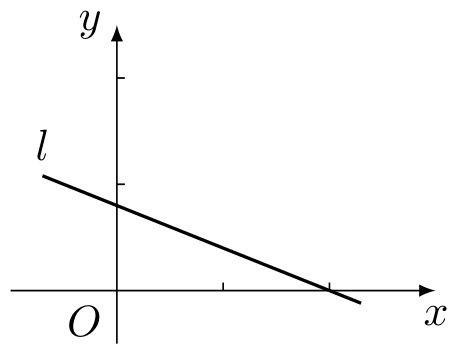
\includegraphics[width=5.3cm]{GaoKao/images/2011/shaanxi_science/q9_fig1.png}
\end{center}

        {\centering\begin{tabular*}{\linewidth}{@{}@{\extracolsep{\fill}}llll@{}}
          \text{A. }\(x\) 和 \(y\) 的相关系数为直线 \(l\) 的斜率  &  \text{B. }\(x\) 和 \(y\) 的相关系数在 \(0\) 到 \(1\) 之间  &  \text{C. }当 \(n\) 为偶数时，分布在 \(l\) 两侧的样本点的个数一定相同  &  \text{D. }直线 \(l\) 过点 \((\bar{x}, \bar{y})\)
        \end{tabular*}\par}

        \item 甲、乙两人一起去游“2011西安世园会”，他们约定：各自独立地从 \(1\) 到 \(6\) 号景点中任选 \(4\) 个进行游览，每个景点参观 \(1\text{ 小时}\)，则最后 \(1\text{ 小时}\) 他们同在一个景点的概率是（\quad）

        {\centering\begin{tabular*}{\linewidth}{@{}@{\extracolsep{\fill}}llll@{}}
          \text{A. }\( \frac{1}{36} \)  &  \text{B. }\( \frac{1}{9} \)  &  \text{C. }\( \frac{5}{36} \)  &  \text{D. }\( \frac{1}{6} \)
        \end{tabular*}\par}

    \end{enumerate}

\end{description}

\begin{description}

    \item[二、填空题]

    \begin{enumerate}[leftmargin=5pt]

      \addtocounter{enumi}{+10}

        \item 设 \(f(x)=\begin{cases}
\lg x, & x>0,\\
x+\int_{0}^{a} 3t^{2}\,dt, & x\leqslant 0
\end{cases}\)，若 \(f(f(1))=1\)，则 \(a=\rule[-0.3ex]{3em}{0.4pt}\).

        \item 设 \(n \in \mathbb{N}^*\)，一元二次方程 \(x^2 - 4x + n = 0\) 有整数根的充要条件是 \(n = \)\rule[-0.3ex]{3em}{0.4pt}.

        \item 观察下列等式 \(1 = 1\)，\(2 + 3 + 4 = 9\)，\(3 + 4 + 5 + 6 + 7 = 25\)，\(4 + 5 + 6 + 7 + 8 + 9 + 10 = 49\). 照此规律，第 \(n\) 个等式应为\rule[-0.3ex]{3em}{0.4pt}.

        \item 植树节某班 \(20\) 名同学在一段直线公路一侧植树，每人植一棵，相邻两棵树相距 \(10\text{ 米}\)，开始时需将树苗集中放置在某一树坑旁边，使每位同学从各自树坑出发前来领取树苗往返所走的路程总和最小，这个最小值为\rule[-0.3ex]{3em}{0.4pt}\(\text{米}\).

    \end{enumerate}

\end{description}

\begin{description}

    \item[三、选做题]

    \begin{enumerate}[leftmargin=5pt]

      \addtocounter{enumi}{+14}

        \item \textbf{【选修4-5：不等式选讲】}

若关于 \(x\) 的不等式 \(\left|a\right| \geqslant \left|x + 1\right| + \left|x - 2\right|\) 存在实数解，则实数 \(a\) 的取值范围是\rule[-0.3ex]{3em}{0.4pt}.

        \item 如图，\(\angle B = \angle D\)，\(AE \perp BC\)，\(\angle ACD = 90^{\circ}\)，且 \(AB = 6\)，\(AC = 4\)，\(AD = 12\)，则 \(BE =\rule[-0.3ex]{3em}{0.4pt}\).

\begin{center}
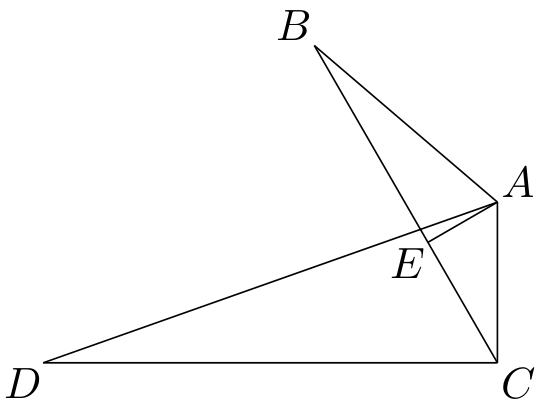
\includegraphics[width=6.8cm]{GaoKao/images/2011/shaanxi_science/q15_fig1.png}
\end{center}

        \item \textbf{【选修4-4：坐标系与参数方程】}

直角坐标系 \(xOy\) 中，以原点为极点，\(x\) 轴正半轴为极轴建立极坐标系，设点 \(A\)，\(B\) 分别在曲线 \( C_{1}:\begin{cases}
x=3+\cos\theta,\\
y=4+\sin\theta,
\end{cases} \)（\(\theta\) 为参数）和曲线 \( C_{2}:\rho=1 \) 上，则 \( |AB| \) 的最小值为\rule[-0.3ex]{3em}{0.4pt}.

    \end{enumerate}

\end{description}

\begin{description}

    \item[四、解答题]

    \begin{enumerate}[leftmargin=5pt]

      \addtocounter{enumi}{+17}

        \item 如图，在 \(\triangle ABC\) 中，\(\angle ABC = 60^{\circ}\)，\(\angle BAC = 90^{\circ}\)，\(AD\) 是 \(BC\) 上的高，沿 \(AD\) 把 \(\triangle ABD\) 折起，使 \(\angle BDC = 90^{\circ}\).
\begin{enumerate}
\item 证明：平面 \(ADB\perp\) 平面 \(BDC\)；
\item 设 \(E\) 为 \(BC\) 的中点，求 \(\overrightarrow{AE}\) 与 \(\overrightarrow{DB}\) 夹角的余弦值.
\end{enumerate}

\begin{center}
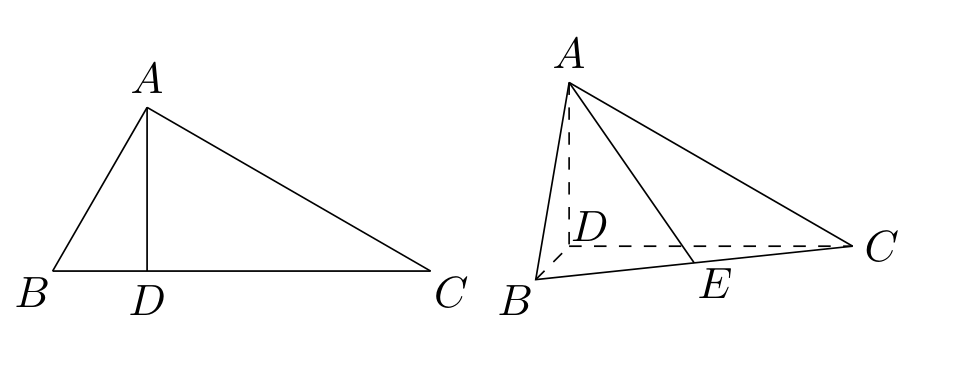
\includegraphics[width=10.5cm]{GaoKao/images/2011/shaanxi_science/q16_fig1.png}
\end{center}

        \item 如图，设 \(P\) 是圆 \(x^{2} + y^{2} = 25\) 上的动点，点 \(D\) 是 \(P\) 在 \(x\) 轴上的投影，\(M\) 为 \(PD\) 上一点，且 \(|MD| = \frac{4}{5} |PD|\).
\begin{enumerate}
\item 当 \(P\) 在圆上运动时，求点 \(M\) 的轨迹 \(C\) 的方程；
\item 求过点 \( (3,0) \) 且斜率为 \( \frac{4}{5} \) 的直线被 \(C\) 所截线段的长度.
\end{enumerate}

\begin{center}
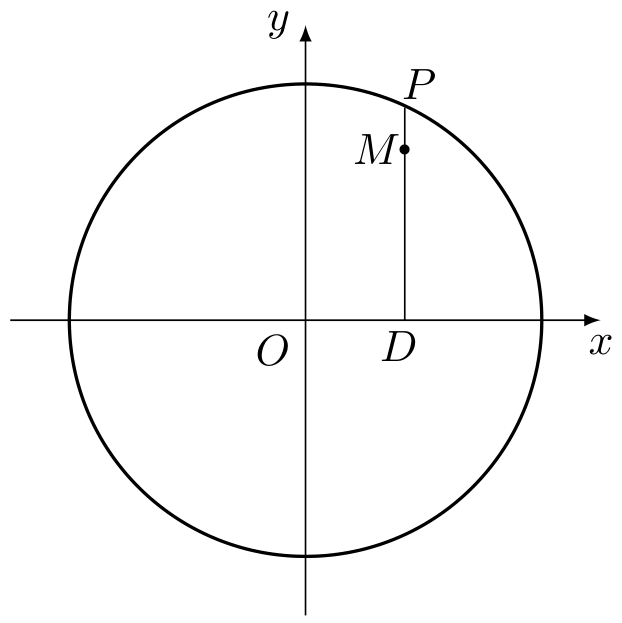
\includegraphics[width=7.7cm]{GaoKao/images/2011/shaanxi_science/q17_fig1.png}
\end{center}

        \item 叙述并证明余弦定理.

        \item 如图，从点 \(P_{1}(0,0)\) 作 \(x\) 轴的垂线交曲线 \(y = {\mathrm{e}}^{x}\) 于点 \(Q_{1}(0,1)\)，曲线在 \(Q_{1}\) 点处的切线与 \(x\) 轴交于点 \(P_{2}\)，再从 \(P_{2}\) 作 \(x\) 轴的垂线交曲线于点 \(Q_{2}\)，依次重复上述过程得到一系列点：\(P_{1}\)，\(Q_{1}\)；\(P_{2}\)，\(Q_{2}\)；\(\cdots\)；\(P_{n}\)，\(Q_{n}\)，记 \(P_{k}\) 点的坐标为 \((x_{k}, 0)\)（\(k = 1, 2, \cdots, n\)）.
\begin{enumerate}
\item 试求 \(x_{k}\) 与 \(x_{k-1}\) 的关系（\(2 \leqslant k \leqslant n\)）；
\item 求 \(\left|P_{1}Q_{1}\right|+\left|P_{2}Q_{2}\right|+\left|P_{3}Q_{3}\right|+\cdots+\left|P_{n}Q_{n}\right|\).
\end{enumerate}

\begin{center}
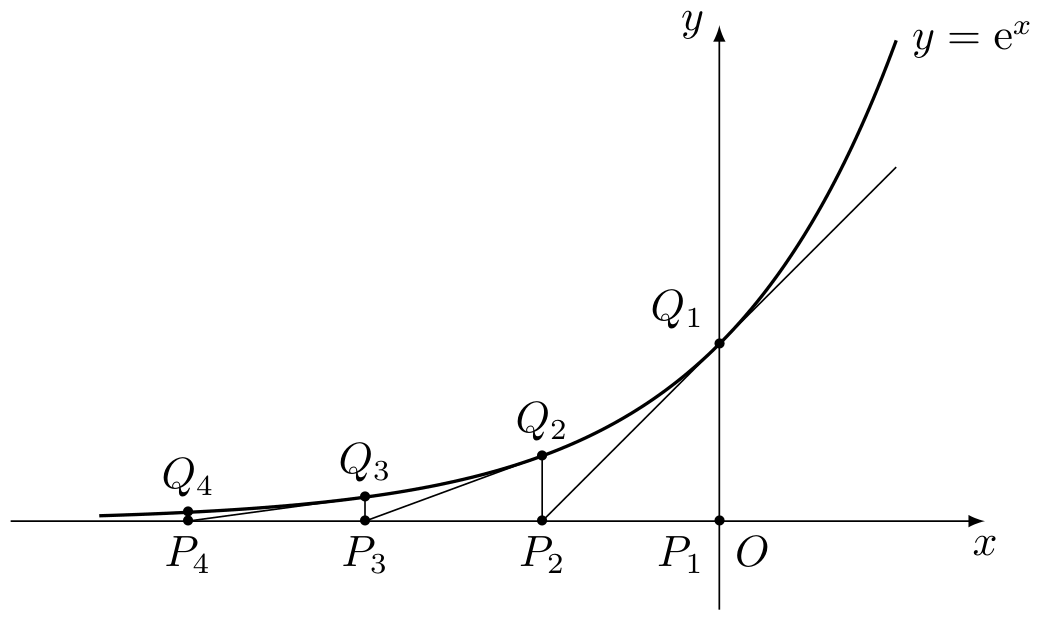
\includegraphics[width=9.9cm]{GaoKao/images/2011/shaanxi_science/q19_fig1.png}
\end{center}

        \item 如图，\(A\) 地到火车站共有两条路径 \(L_{1}\) 和 \(L_{2}\)，据统计，通过两条路径所用的时间互不影响，所用时间落在各时间段内的频率如下表：
\begin{center}
\begin{tabular}{c|ccccc}
\hline
所用时间（分钟） & \(10\sim20\) & \(20\sim30\) & \(30\sim40\) & \(40\sim50\) & \(50\sim60\) \\
\hline
选择 \(L_1\) 的人数 & \(6\) & \(12\) & \(18\) & \(12\) & \(12\) \\
选择 \(L_2\) 的人数 & \(0\) & \(4\) & \(16\) & \(16\) & \(4\) \\
\hline
\end{tabular}
\end{center}
现甲、乙两人分别有 \(40\text{ 分钟}\) 和 \(50\text{ 分钟}\) 时间用于赶往火车站.
\begin{enumerate}
\item 为了尽最大可能在各自允许的时间内赶到火车站，甲和乙应如何选择各自的路径？
\item 用 \(X\) 表示甲、乙两人中在允许的时间内能赶到火车站的人数，针对（1）的选择方案，求 \(X\) 的分布列和数学期望.
\end{enumerate}

\begingroup
\leftskip=0pt\relax
\begin{center}
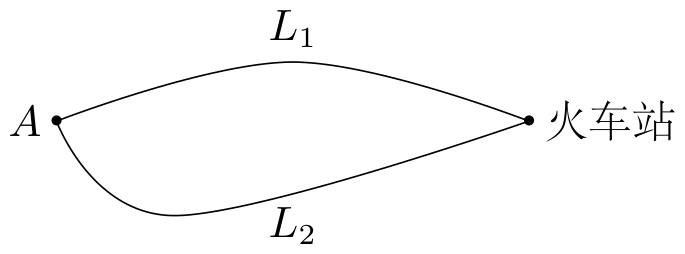
\includegraphics[width=6.9cm]{GaoKao/images/2011/shaanxi_science/q20_fig1.png}
\end{center}
\endgroup

        \item 设函数 \(f(x)\) 定义在 \((0, +\infty)\) 上，\(f(1) = 0\)，导函数 \(f'(x) = \frac{1}{x}\)，\(g(x) = f(x) + f'(x)\).
\begin{enumerate}
\item 求 \(g(x)\) 的单调区间和最小值；
\item 讨论 \(g(x)\) 与 \(g\left(\frac{1}{x}\right)\) 的大小关系；
\item 是否存在 \(x_0 > 0\)，使得 \(|g(x) - g(x_0)| < \frac{1}{2}\) 对任意 \(x > 0\) 成立？若存在，求出 \(x_0\) 的取值范围；若不存在，请说明理由.
\end{enumerate}

    \end{enumerate}

\end{description}


\subsection{2011年陕西卷（文）}\label{gk:2011年陕西卷（文）}

\begin{description}

    \item[一、选择题]

    \begin{enumerate}[leftmargin=5pt]

        \item 设 \(\bm{a}\)，\(\bm{b}\) 是向量，命题“若 \(\bm{a} = -\bm{b}\)，则 \(|\bm{a}| = |\bm{b}|\)”的逆命题是（\quad）

        {\centering\begin{tabular*}{\linewidth}{@{}@{\extracolsep{\fill}}llll@{}}
          \text{A. }若 \(\bm{a} \neq -\bm{b}\)，则 \(|\bm{a}| \neq |\bm{b}|\)  &  \text{B. }若 \(\bm{a} = -\bm{b}\)，则 \(|\bm{a}| \neq |\bm{b}|\)  &  \text{C. }若 \(|\bm{a}| \neq |\bm{b}|\)，则 \(\bm{a} \neq -\bm{b}\)  &  \text{D. }若 \(|\bm{a}| = |\bm{b}|\)，则 \(\bm{a} = -\bm{b}\)
        \end{tabular*}\par}

        \item 设抛物线的顶点在原点，准线方程为 \(x = -2\)，则抛物线的方程是（\quad）

        {\centering\begin{tabular*}{\linewidth}{@{}@{\extracolsep{\fill}}llll@{}}
          \text{A. }\( y^{2} = -8x \)  &  \text{B. }\( y^{2} = -4x \)  &  \text{C. }\( y^{2} = 8x \)  &  \text{D. }\( y^{2} = 4x \)
        \end{tabular*}\par}

        \item 设 \(0 < a < b\)，则下列不等式中正确的是（\quad）

        {\centering\begin{tabular*}{\linewidth}{@{}@{\extracolsep{\fill}}llll@{}}
          \text{A. }\(a < b < \sqrt{ab} < \frac{a + b}{2}\)  &  \text{B. }\(a < \sqrt{ab} < \frac{a + b}{2} < b\)  &  \text{C. }\(a < \sqrt{ab} < b < \frac{a + b}{2}\)  &  \text{D. }\(\sqrt{ab} < a < \frac{a + b}{2} < b\)
        \end{tabular*}\par}

        \item 函数 \( y = x^{\frac{1}{3}} \) 的图象是（\quad）

        {\centering\begin{tabular*}{\linewidth}{@{}@{\extracolsep{\fill}}cccc@{}}
          \text{A. }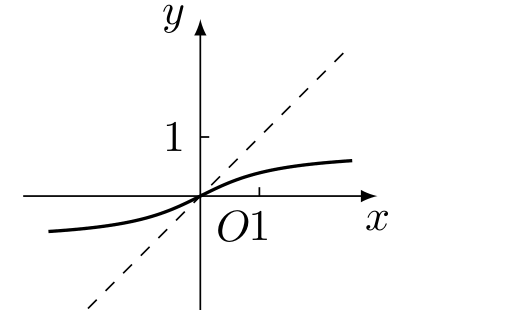
\includegraphics[width=0.15\paperwidth]{GaoKao/images/2011/shaanxi_liberal/q4_optA_clean.png}  &  \text{B. }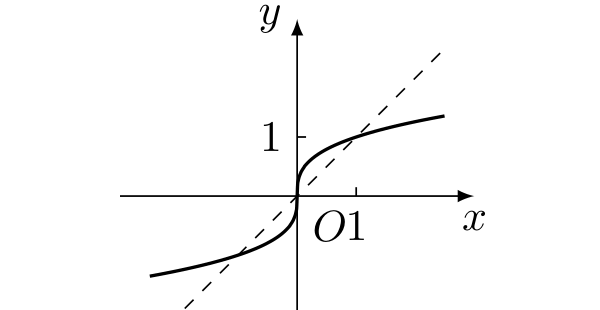
\includegraphics[width=0.15\paperwidth]{GaoKao/images/2011/shaanxi_liberal/q4_optB_clean.png}  &  \text{C. }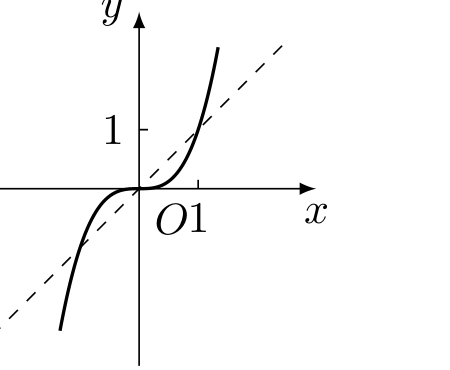
\includegraphics[width=0.15\paperwidth]{GaoKao/images/2011/shaanxi_liberal/q4_optC_clean.png}  &  \text{D. }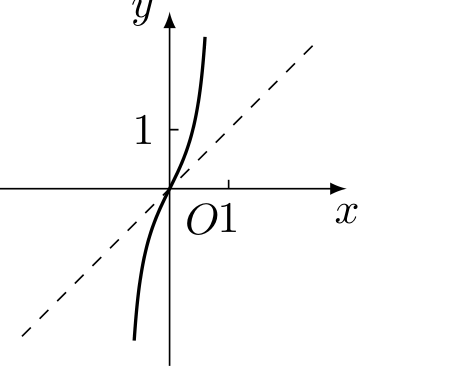
\includegraphics[width=0.15\paperwidth]{GaoKao/images/2011/shaanxi_liberal/q4_optD_clean.png}
        \end{tabular*}\par}

        \item 某几何体的三视图如图所示，则它的体积是（\quad）

\begin{center}
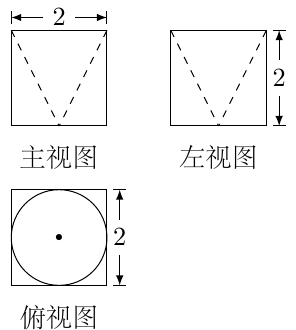
\includegraphics[width=2.4cm]{GaoKao/images/2011/shaanxi_liberal/q5_fig1.png}
\end{center}

        {\centering\begin{tabular*}{\linewidth}{@{}@{\extracolsep{\fill}}llll@{}}
          \text{A. }\(8 - \frac{2\pi}{3}\)  &  \text{B. }\(8 - \frac{\pi}{3}\)  &  \text{C. }\(8 - 2\pi\)  &  \text{D. }\(\frac{2\pi}{3}\)
        \end{tabular*}\par}

        \item 方程 \( |x| = \cos x \) 在 \((- \infty, + \infty)\) 内（\quad）

        {\centering\begin{tabular*}{\linewidth}{@{}@{\extracolsep{\fill}}llll@{}}
          \text{A. }没有根  &  \text{B. }有且仅有一个根  &  \text{C. }有且仅有两个根  &  \text{D. }有无穷多个根
        \end{tabular*}\par}

        \item 下面的框图中，当 \(x_{1} = 6\)，\(x_{2} = 9\)，\(p = 8.5\) 时，\(x_{3}\) 等于（\quad）

\begin{center}
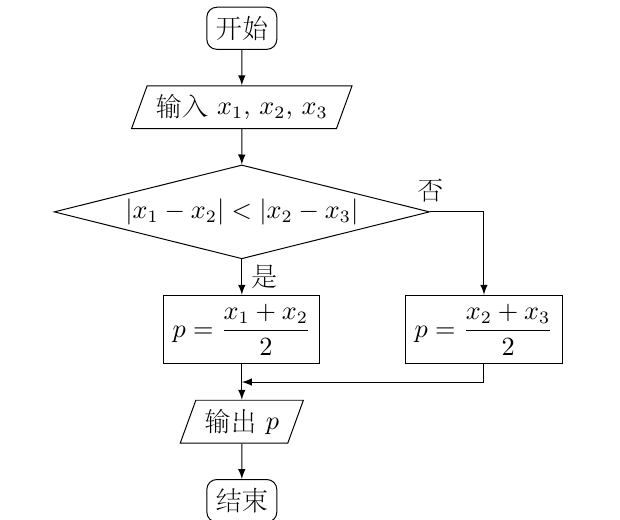
\includegraphics[width=0.52\linewidth]{GaoKao/images/2011/shaanxi_liberal/q7_fig1.png}
\end{center}

        {\centering\begin{tabular*}{\linewidth}{@{}@{\extracolsep{\fill}}llll@{}}
          \text{A. }7  &  \text{B. }8  &  \text{C. }10  &  \text{D. }11
        \end{tabular*}\par}

        \item 设集合 \(M = \{y \mid y = |\cos^2 x - \sin^2 x|, x \in \mathbb{R}\}\)，\(N = \left\{x \mid \left|\frac{x}{\i}\right| < 1,\ \i\text{ 为虚数单位},\ x \in \mathbb{R}\right\}\)，则 \(M \cap N\) 为（\quad）

        {\centering\begin{tabular*}{\linewidth}{@{}@{\extracolsep{\fill}}llll@{}}
          \text{A. }\((0,1)\)  &  \text{B. }\((0,1]\)  &  \text{C. }\([0,1)\)  &  \text{D. }\([0,1]\)
        \end{tabular*}\par}

        \item 设 \((x_{1}, y_{1})\)，\((x_{2}, y_{2})\)，\(\cdots\)，\((x_{n}, y_{n})\) 是变量 \(x\) 和 \(y\) 的 \(n\) 个样本点，直线 \(l\) 是由这些样本点通过最小二乘法得到的线性回归直线（如图），以下结论中正确的是（\quad）

\begin{center}
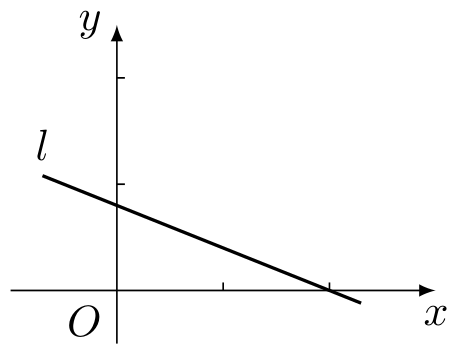
\includegraphics[width=5.3cm]{GaoKao/images/2011/shaanxi_liberal/q9_fig1.png}
\end{center}

        {\centering\begin{tabular*}{\linewidth}{@{}@{\extracolsep{\fill}}llll@{}}
          \text{A. }直线 \(l\) 过点 \((\overline{x}, \overline{y})\)  &  \text{B. }\(x\) 和 \(y\) 的相关系数为直线 \(l\) 的斜率  &  \text{C. }\(x\) 和 \(y\) 的相关系数在 \(0\) 到 \(1\) 之间  &  \text{D. }当 \(n\) 为偶数时，分布在 \(l\) 两侧的样本点的个数一定相同
        \end{tabular*}\par}

        \item 植树节某班 \(20\) 名同学在一段直线公路一侧植树，每人植一棵，相邻两棵树相距 \(10\text{ 米}\)，开始时需将树苗集中放置在某一树坑旁边，现将树坑从 \(1\) 到 \(20\) 依次编号，为使各位同学从各自树坑前来领取树苗所走的路程总和最小，树苗可以放置的两个最佳坑位的编号为（\quad）

        {\centering\begin{tabular*}{\linewidth}{@{}@{\extracolsep{\fill}}llll@{}}
          \text{A. }\(1\) 和 \(20\)  &  \text{B. }\(9\) 和 \(10\)  &  \text{C. }\(9\) 和 \(11\)  &  \text{D. }\(10\) 和 \(11\)
        \end{tabular*}\par}

    \end{enumerate}

\end{description}

\begin{description}

    \item[二、填空题]

    \begin{enumerate}[leftmargin=5pt]

      \addtocounter{enumi}{+10}

        \item 设函数 \( f(x) = \begin{cases}
\lg x, & x > 0,\\
10^x, & x \leqslant 0.
\end{cases} \) 则 \( f(f(-2)) = \)\rule[-0.3ex]{3em}{0.4pt}.

        \item 如图，点 \((x, y)\) 在四边形 \(ABCD\) 内部和边界上运动，那么 \(2x - y\) 的最小值为\rule[-0.3ex]{3em}{0.4pt}.

\begin{center}
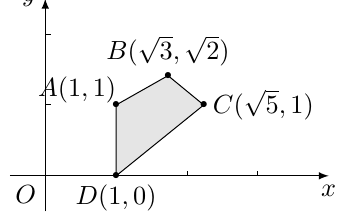
\includegraphics[width=4.4cm]{GaoKao/images/2011/shaanxi_liberal/q12_fig1.png}
\end{center}

        \item 观察下列等式 \(1 = 1\)，\(2 + 3 + 4 = 9\)，\(3 + 4 + 5 + 6 + 7 = 25\)，\(4 + 5 + 6 + 7 + 8 + 9 + 10 = 49\)，\(\dots\). 照此规律，第五个等式应为\rule[-0.3ex]{3em}{0.4pt}.

        \item 设 \(n \in \mathbb{N}_{+}\)，一元二次方程 \(x^{2} - 4x + n = 0\) 有整数根的充要条件是 \(n=\)\rule[-0.3ex]{3em}{0.4pt}.

    \end{enumerate}

\end{description}

\begin{description}

    \item[三、选做题]

    \begin{enumerate}[leftmargin=5pt]

      \addtocounter{enumi}{+14}

        \item \textbf{【选修4-5：不等式选讲】}

若不等式 \( |x+1|+|x-2|\geqslant a \) 对任意 \( x\in\mathbb{R} \) 恒成立，则 \(a\) 的取值范围是\rule[-0.3ex]{3em}{0.4pt}.

        \item 如图，\( \angle B = \angle D\)，\( AE \perp BC\)，\( \angle ACD = 90^{\circ}\)，且 \(AB = 6\)，\(AC = 4\)，\(AD = 12\)，则 \(AE =\)\rule[-0.3ex]{3em}{0.4pt}.

\begin{center}
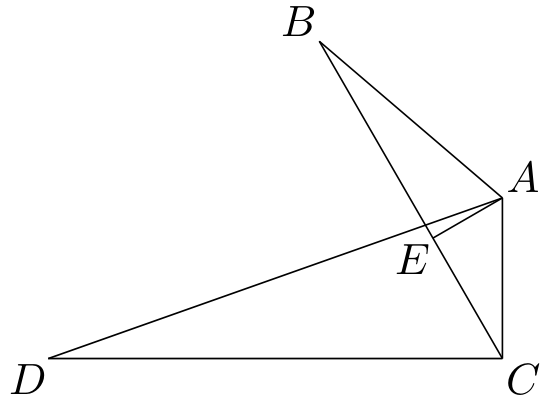
\includegraphics[width=6.8cm]{GaoKao/images/2011/shaanxi_liberal/q15_fig1.png}
\end{center}

        \item \textbf{【选修4-4：坐标系与参数方程】}

直角坐标系 \(xOy\) 中，以原点为极点，\(x\) 轴正半轴为极轴建立极坐标系，设点 \(A\)，\(B\) 分别在曲线 \(C_1: \begin{cases}
x = 3 + \cos \theta,\\
y = \sin \theta,
\end{cases}\) （\(\theta\) 为参数）和曲线 \(C_2: \rho = 1\) 上，则 \(|AB|\) 的最小值为\rule[-0.3ex]{3em}{0.4pt}.

    \end{enumerate}

\end{description}

\begin{description}

    \item[四、解答题]

    \begin{enumerate}[leftmargin=5pt]

      \addtocounter{enumi}{+17}

        \item 如图，在 \(\triangle ABC\) 中，\(\angle ABC = 45^{\circ}\)，\(\angle BAC = 90^{\circ}\)，\(AD\) 是 \(BC\) 上的高，沿 \(AD\) 把 \(\triangle ABD\) 折起，使 \(\angle BDC = 90^{\circ}\).

\begin{enumerate}
\item 证明：平面 \(ADB \perp\) 平面 \(BDC\)；
\item 若 \(BD = 1\)，求三棱锥 \(D - ABC\) 的表面积.
\end{enumerate}

\begin{center}
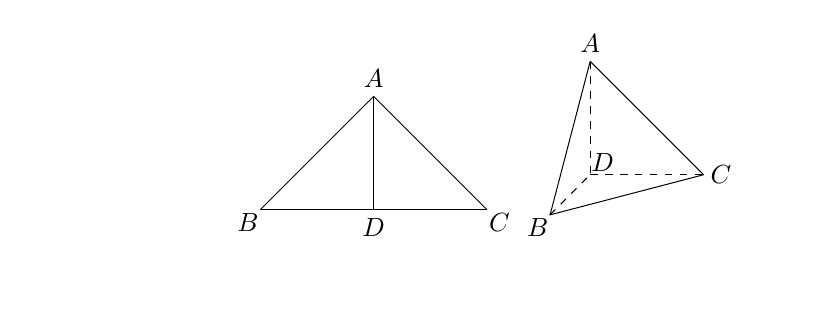
\includegraphics[width=10.5cm]{GaoKao/images/2011/shaanxi_liberal/q16_fig1.png}
\end{center}

        \item 设椭圆 \(C: \frac{x^2}{a^2} + \frac{y^2}{b^2} = 1\)（\(a > b > 0\)）过点 \((0,4)\)，离心率为 \(\frac{3}{5}\).

\begin{enumerate}
\item 求 \(C\) 的方程；
\item 求过点 \((3,0)\) 且斜率为 \(\frac{4}{5}\) 的直线被 \(C\) 所截线段的中点坐标.
\end{enumerate}

        \item 叙述并证明余弦定理.

        \item 如图，从点 \(P_{1}(0,0)\) 作 \(x\) 轴的垂线交曲线 \(y = {\mathrm{e}}^{x}\) 于点 \(Q_{1}(0,1)\)，曲线在 \(Q_{1}\) 点处的切线与 \(x\) 轴交于点 \(P_{2}\)，再从 \(P_{2}\) 作 \(x\) 轴的垂线交曲线于点 \(Q_{2}\)，依次重复上述过程得到一系列点：\(P_{1}\)，\(Q_{1}\)；\(P_{2}\)，\(Q_{2}\)；\(\cdots\)；\(P_{n}\)，\(Q_{n}\)，记 \(P_{k}\) 点的坐标为 \((x_{k}, 0)\)（\(k = 1\)，\(2\)，\(\cdots\)，\(n\)）.

\begin{enumerate}
\item 试求 \(x_{k}\) 与 \(x_{k-1}\) 的关系（\(2 \leqslant k \leqslant n\)）；
\item 求 \( \left|P_{1}Q_{1}\right|+\left|P_{2}Q_{2}\right|+\left|P_{3}Q_{3}\right|+\cdots+\left|P_{n}Q_{n}\right| \).
\end{enumerate}

\begin{center}
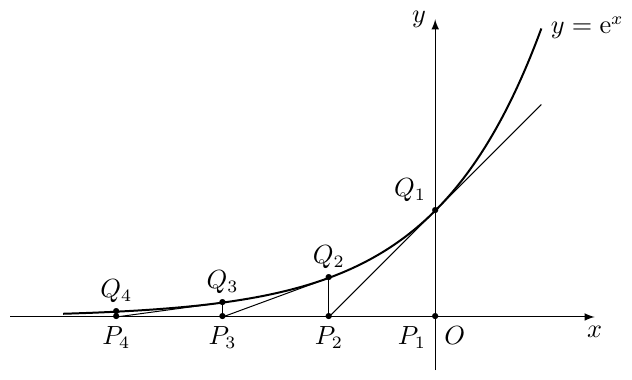
\includegraphics[width=10.3cm]{GaoKao/images/2011/shaanxi_liberal/q19_fig1.png}
\end{center}

        \item 如图，\(A\) 地到火车站共有两条路径 \(L_{1}\) 和 \(L_{2}\)，现随机抽取 \(100\) 位从 \(A\) 地到达火车站的人进行调查，调查结果如下：

\begin{center}
\begin{tabular}{c|ccccc}
\hline
所用时间（分钟） & \(10\sim20\) & \(20\sim30\) & \(30\sim40\) & \(40\sim50\) & \(50\sim60\) \\
\hline
选择 \(L_{1}\) 的人数 & \(6\) & \(12\) & \(18\) & \(12\) & \(12\) \\
选择 \(L_{2}\) 的人数 & \(0\) & \(4\) & \(16\) & \(16\) & \(4\) \\
\hline
\end{tabular}
\end{center}

\begin{enumerate}
\item 试估计 \(40\text{ 分钟}\) 内不能赶到火车站的概率；
\item 分别求通过路径 \(L_{1}\) 和 \(L_{2}\) 所用时间落在上表中各时间段内的频率；
\item 现甲，乙两人分别有 \(40\text{ 分钟}\) 和 \(50\text{ 分钟}\) 时间用于赶往火车站，为了尽最大可能在允许的时间内赶到火车站，试通过计算说明，他们应如何选择各自的路径.
\end{enumerate}

\begin{center}
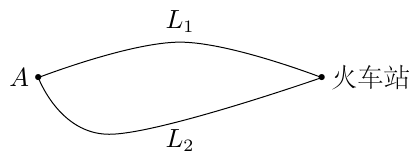
\includegraphics[width=7.4cm]{GaoKao/images/2011/shaanxi_liberal/q20_fig1.png}
\end{center}

        \item 设 \(f(x) = \ln x\)，\(g(x) = f(x) + f'(x)\).

\begin{enumerate}
\item 求 \(g(x)\) 的单调区间和最小值；
\item 讨论 \(g(x)\) 与 \(g\left(\frac{1}{x}\right)\) 的大小关系；
\item 求 \(a\) 的取值范围，使得 \(g(a) - g(x) < \frac{1}{a}\) 对任意 \(x > 0\) 成立.
\end{enumerate}

    \end{enumerate}

\end{description}


\subsection{2011年天津卷（理）}\label{gk:2011年天津卷（理）}

\begin{description}

    \item[一、选择题]

    \begin{enumerate}[leftmargin=5pt]

        \item \(i\) 是虚数单位，复数 \( \frac{1-3\i}{1-\i}= \)（\quad）

        {\centering\begin{tabular*}{\linewidth}{@{}@{\extracolsep{\fill}}llll@{}}
          \text{A. }\(2 + \i\)  &  \text{B. }\(2 - \i\)  &  \text{C. }\(-1 + 2\i\)  &  \text{D. }\(-1 - 2\i\)
        \end{tabular*}\par}

        \item 设 \(x\)，\(y \in \mathbb{R}\)，则“\(x \geqslant 2\) 且 \(y \geqslant 2\)”是“\(x^2 + y^2 \geqslant 4\)”的（\quad）

        {\centering\begin{tabular*}{\linewidth}{@{}@{\extracolsep{\fill}}llll@{}}
          \text{A. }充分而不必要条件  &  \text{B. }必要而不充分条件  &  \text{C. }充分必要条件  &  \text{D. }既不充分也不必要条件
        \end{tabular*}\par}

        \item 阅读下面的程序框图，运行相应的程序，则输出 \(i\) 的值为（\quad）

\begin{center}
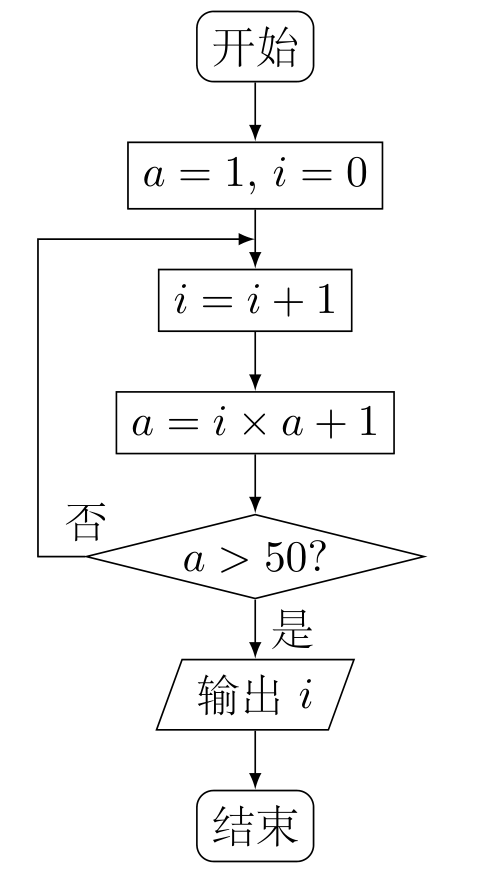
\includegraphics[width=0.70\linewidth]{GaoKao/images/2011/tianjin_science/q3_fig1.png}
\end{center}

        {\centering\begin{tabular*}{\linewidth}{@{}@{\extracolsep{\fill}}llll@{}}
          \text{A. }3  &  \text{B. }4  &  \text{C. }5  &  \text{D. }6
        \end{tabular*}\par}

        \item 已知 \( \{a_{n}\} \) 为等差数列，其公差为 \(-2\)，且 \( a_{7} \) 是 \( a_{3} \) 与 \( a_{9} \) 的等比中项，\( S_{n} \) 为 \( \{a_{n}\} \) 的前 \(n\) 项和，\( n \in \mathbb{N}^{*} \)，则 \(S_{10}\) 的值为（\quad）

        {\centering\begin{tabular*}{\linewidth}{@{}@{\extracolsep{\fill}}llll@{}}
          \text{A. }\(-110\)  &  \text{B. }\(-90\)  &  \text{C. }90  &  \text{D. }110
        \end{tabular*}\par}

        \item 在 \(\left(\frac{\sqrt{x}}{2} - \frac{2}{\sqrt{x}}\right)^{6}\) 的二项展开式中，\(x^{2}\) 的系数为（\quad）

        {\centering\begin{tabular*}{\linewidth}{@{}@{\extracolsep{\fill}}llll@{}}
          \text{A. }\(-\frac{15}{4}\)  &  \text{B. }\( \frac{15}{4} \)  &  \text{C. }\(-\frac{3}{8}\)  &  \text{D. }\(\frac{3}{8}\)
        \end{tabular*}\par}

        \item 如图所示，在 \(\triangle ABC\) 中，\(D\) 是边 \(AC\) 上的点，且 \(AB = AD\)，\(2AB = \sqrt{3}BD\)，\(BC = 2BD\)，则 \(\sin C\) 的值为（\quad）

\begin{center}
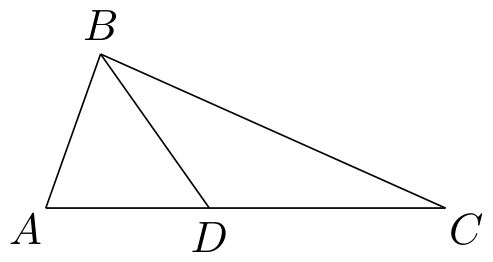
\includegraphics[width=6.1cm]{GaoKao/images/2011/tianjin_science/q6_fig1.png}
\end{center}

        {\centering\begin{tabular*}{\linewidth}{@{}@{\extracolsep{\fill}}llll@{}}
          \text{A. }\(\frac{\sqrt{3}}{3}\)  &  \text{B. }\(\frac{\sqrt{3}}{6}\)  &  \text{C. }\(\frac{\sqrt{6}}{3}\)  &  \text{D. }\(\frac{\sqrt{6}}{6}\)
        \end{tabular*}\par}

        \item 已知 \(a = 5^{\log_{2} 3^{4}}\)，\(b = 5^{\log_{4} 3^{6}}\)，\(c = \left(\frac{1}{5}\right)^{\log_{3} 0.3}\)，则（\quad）

        {\centering\begin{tabular*}{\linewidth}{@{}@{\extracolsep{\fill}}llll@{}}
          \text{A. }\(a > b > c\)  &  \text{B. }\(b > a > c\)  &  \text{C. }\(a > c > b\)  &  \text{D. }\(c > a > b\)
        \end{tabular*}\par}

        \item 对实数 \(a\) 与 \(b\)，定义运算“\(\otimes\)”： \(a \otimes b = \begin{cases}
a, & a - b \leqslant 1,\\
b, & a - b > 1.
\end{cases}\) 设函数 \(f(x) = (x^2 - 2) \otimes (x - x^2)\)，\(x \in \mathbb{R}\). 若函数 \(y = f(x) - c\) 的图象与 \(x\) 轴恰有两个公共点，则实数 \(c\) 的取值范围是（\quad）

        {\centering\begin{tabular*}{\linewidth}{@{}@{\extracolsep{\fill}}llll@{}}
          \text{A. }\((- \infty, -2] \cup \left(-1, \frac{3}{2}\right)\)  &  \text{B. }\((-\infty, -2] \cup \left(-1, -\frac{3}{4}\right)\)  &  \text{C. }\(\left(-1, \frac{1}{4}\right) \cup \left(\frac{1}{4}, +\infty\right)\)  &  \text{D. }\(\left(-1, -\frac{3}{4}\right) \cup \left[\frac{1}{4}, +\infty\right)\)
        \end{tabular*}\par}

    \end{enumerate}

\end{description}

\begin{description}

    \item[二、填空题]

    \begin{enumerate}[leftmargin=5pt]

      \addtocounter{enumi}{+8}

        \item 一支田径队有男运动员 48 人，女运动员 36 人，若用分层抽样的方法从该队的全体运动员中抽取一个容量为 21 的样本，则抽取男运动员的人数为\rule[-0.3ex]{3em}{0.4pt}.

        \item 一个几何体的三视图如图所示（单位：m），则这个几何体的体积为\rule[-0.3ex]{3em}{0.4pt} \(\text{m}^{3}\).

\begin{center}
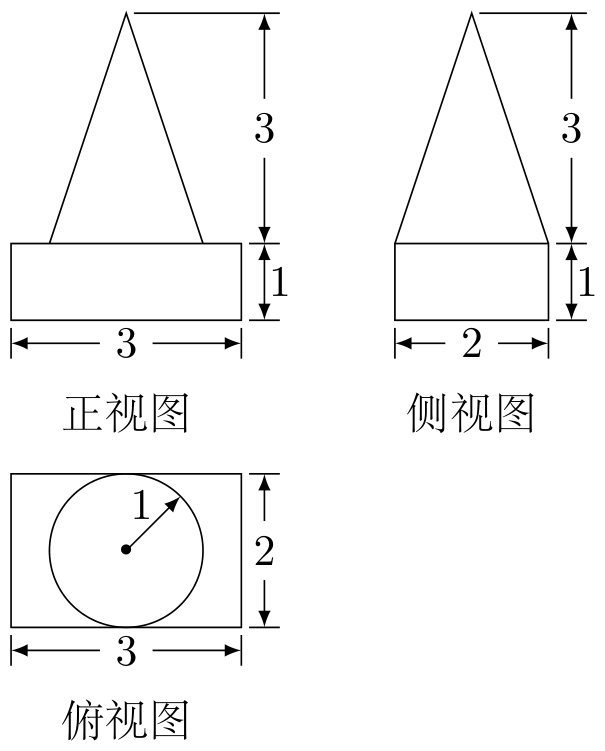
\includegraphics[width=5.9cm]{GaoKao/images/2011/tianjin_science/q10_fig1.png}
\end{center}

        \item 已知抛物线 \(C\) 的参数方程为
\(\begin{cases}
x = 8t^{2},\\
y = 8t,
\end{cases}\)
（\(t\) 为参数），若斜率为 1 的直线经过抛物线 \(C\) 的焦点，且与圆 \( (x - 4)^{2} + y^{2} = r^{2} \) （\(r > 0\)）相切，则 \(r =\)\rule[-0.3ex]{3em}{0.4pt}.

        \item 如图，已知圆中两条弦 \(AB\) 与 \(CD\) 相交于点 \(F\)，\(E\) 是 \(AB\) 延长线上一点，且 \(DF = CF = \sqrt{2}\)，\(AF:FB:BE = 4:2:1\).
若 \(CE\) 与圆相切，则 \(CE\) 的长为\rule[-0.3ex]{3em}{0.4pt}.

\begin{center}
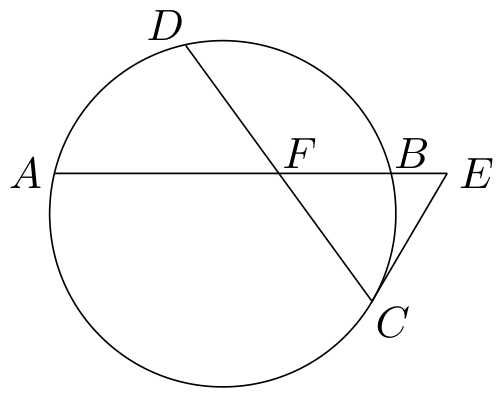
\includegraphics[width=6.2cm]{GaoKao/images/2011/tianjin_science/q12_fig1.png}
\end{center}

        \item 已知集合 \(A = \{x \in \mathbb{R} \mid |x + 3| + |x - 4| \leqslant 9\}\)，\(B = \left\{x \in \mathbb{R} \mid x = 4t + \frac{1}{t} - 6, t \in (0, +\infty)\right\}\)，则集合 \(A \cap B = \)\rule[-0.3ex]{3em}{0.4pt}.

        \item 已知直角梯形 \(ABCD\) 中，\(AD \parallel BC\)，\(\angle ADC = 90^{\circ}\)，\(AD = 2\)，\(BC = 1\)，\(P\) 是腰 \(DC\) 上的动点，则 \(\left|\overrightarrow{PA} + 3\overrightarrow{PB}\right|\) 的最小值为\rule[-0.3ex]{3em}{0.4pt}.

    \end{enumerate}

\end{description}

\begin{description}

    \item[三、解答题]

    \begin{enumerate}[leftmargin=5pt]

      \addtocounter{enumi}{+14}

        \item 已知函数 \( f(x) = \tan \left(2x + \frac{\pi}{4}\right) \).
\begin{enumerate}
\item 求 \( f(x) \) 的定义域与最小正周期；
\item 设 \(\alpha \in (0, \frac{\pi}{4})\)，若 \(f\left(\frac{\alpha}{2}\right) = 2\cos 2\alpha\)，求 \(\alpha\) 的大小.
\end{enumerate}

        \item 学校游园活动有这样一个游戏项目：甲箱子里装有3个白球，2个黑球，乙箱子里装有1个白球，2个黑球，这些球除颜色外完全相同. 每次游戏从这两个箱子里各随机摸出2个球，若摸出的白球不少于2个，则获奖. （每次游戏结束后将球放回原箱）
\begin{enumerate}
\item 求在一次游戏中
\begin{enumerate}
    \item 摸出 3 个白球的概率；
    \item 获奖的概率.
\end{enumerate}
\item 求在两次中获奖次数 X 的分布列及数学期望 \( E(X) \).
\end{enumerate}

        \item 如图，在三棱柱 \(ABC - A_{1}B_{1}C_{1}\) 中，\(H\) 是正方形 \(AA_{1}B_{1}B\) 的中心，\(AA_{1} = 2\sqrt{2}\)，\(C_{1}H \perp\) 平面 \(AA_{1}B_{1}B\)，且 \(C_{1}H = \sqrt{5}\).
\begin{enumerate}
\item 求异面直线 \(AC\) 与 \(A_{1}B_{1}\) 所成角的余弦值；
\item 求二面角 \(A - A_{1}C_{1} - B_{1}\) 的正弦值；
\item 设 \(N\) 为棱 \(B_{1}C_{1}\) 的中点，点 \(M\) 在平面 \(AA_{1}B_{1}B\) 内，且 \(MN \perp\) 平面 \(A_{1}B_{1}C_{1}\)，求线段 \(BM\) 的长.
\end{enumerate}
\begin{center}
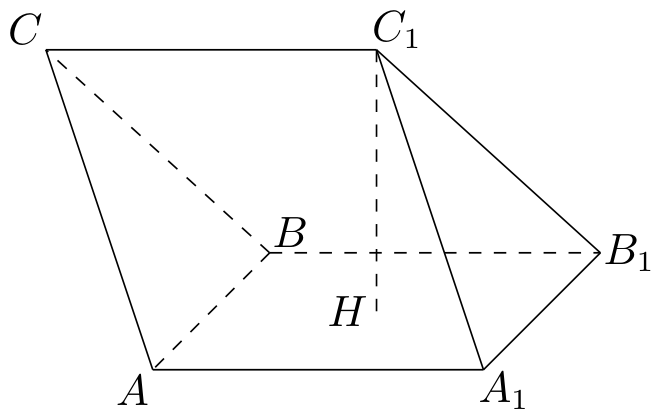
\includegraphics[width=6.5cm]{GaoKao/images/2011/tianjin_science/q17_fig1.png}
\end{center}

        \item 已知 \(a > 0\)，函数 \(f(x) = \ln x - ax^2\)，\(x > 0\).（\(f(x)\) 的图象连续不断）
\begin{enumerate}
\item 求 \( f(x) \) 的单调区间；
\item 当 \(a = \frac{1}{8}\) 时，证明：存在 \(x_0 \in (2, +\infty)\)，使 \(f(x_0) = f\left(\frac{3}{2}\right)\).
\item 若存在均属于区间 \([1,3]\) 的 \(\alpha\)，\(\beta\)，且 \(\beta - \alpha \geqslant 1\)，使 \(f(\alpha) = f(\beta)\). 证明： \(\frac{\ln 3 - \ln 2}{5} \leqslant a \leqslant \frac{\ln 2}{3}\).
\end{enumerate}

        \item 已知数列 \(\{a_{n}\}\) 与 \(\{b_{n}\}\) 满足： \(b_{n}a_{n} + a_{n + 1} + b_{n + 1}a_{n + 2} = 0\)，\(b_{n} = \frac{3 + (-1)^{n}}{2}\)，\(n \in \mathbb{N}^{*}\)，且 \(a_{1} = 2\)，\(a_{2} = 4\)，
\begin{enumerate}
\item 求 \(a_{3}\)，\(a_{4}\)，\(a_{5}\) 的值；
\item 设 \(c_{n} = a_{2n - 1} + a_{2n + 1}\)，\(n \in \mathbb{N}^{*}\)，证明： \(\{c_{n}\}\) 是等比数列；
\item 设 \(S_{k} = a_{2} + a_{4} + \dots + a_{2k}\)，\(k \in \mathbb{N}^{*}\)，证明： \(\sum_{k=1}^{n} \frac{S_{k}}{a_{k}} < \frac{7}{6}\)（\(n \in \mathbb{N}^{*}\)）.
\end{enumerate}

        \item 在平面直角坐标系 \(xOy\) 中，点 \(P(a,b)\) （\(a > b > 0\)） 为动点，\(F_{1}\)，\(F_{2}\) 分别为椭圆 \(\frac{x^2}{a^2} + \frac{y^2}{b^2} = 1\) 的左，右焦点. 已知 \(\triangle F_1PF_2\) 为等腰三角形.
\begin{enumerate}
\item 求椭圆的离心率 \(e\)；
\item 设直线 \(PF_{2}\) 与椭圆相交于 \(A\)，\(B\) 两点，\(M\) 是直线 \(PF_{2}\) 上的点，满足 \(\overrightarrow{AM} \cdot \overrightarrow{BM} = -2\)，求点 \(M\) 的轨迹方程.
\end{enumerate}

    \end{enumerate}

\end{description}


\subsection{2011年天津卷（文）}\label{gk:2011年天津卷（文）}

\begin{description}

    \item[一、选择题]

    \begin{enumerate}[leftmargin=5pt]

        \item \(\i\) 是虚数单位，复数 \(\frac{1 - 3\i}{1 - \i} =\)（\quad）

        {\centering\begin{tabular*}{\linewidth}{@{}@{\extracolsep{\fill}}llll@{}}
          \text{A. }\(2 - \i\)  &  \text{B. }\(2 + \i\)  &  \text{C. }\(-1 - 2\i\)  &  \text{D. }\(-1 + 2\i\)
        \end{tabular*}\par}

        \item 设变量 \(x\)，\(y\) 满足的约束条件 \(\begin{cases}
x\geqslant 1,\\
x+y-4\leqslant 0,\\
x-3y+4\leqslant 0
\end{cases}\)，则目标函数 \(z = 3x - y\) 的最大值为（\quad）

        {\centering\begin{tabular*}{\linewidth}{@{}@{\extracolsep{\fill}}llll@{}}
          \text{A. }\(-4\)  &  \text{B. }\(0\)  &  \text{C. }\( \frac{4}{3} \)  &  \text{D. }\(4\)
        \end{tabular*}\par}

        \item 阅读程序框图，运行相应的程序，若输入 \(x\) 的值为 \(-4\)，则输出 \(y\) 的值为（\quad）

\begin{center}
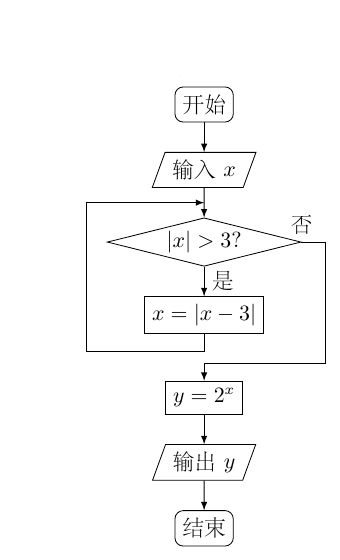
\includegraphics[width=0.70\linewidth]{GaoKao/images/2011/tianjin_liberal/q3_fig1.png}
\end{center}

        {\centering\begin{tabular*}{\linewidth}{@{}@{\extracolsep{\fill}}llll@{}}
          \text{A. }\(0.5\)  &  \text{B. }\(1\)  &  \text{C. }\(2\)  &  \text{D. }\(4\)
        \end{tabular*}\par}

        \item 设集合 \(A = \{x \in \mathbb{R} \mid x - 2 > 0\}\)，\(B = \{x \in \mathbb{R} \mid x < 0\}\)，\(C = \{x \in \mathbb{R} \mid x(x - 2) > 0\}\)，则“\(x \in A \cup B\)”是“\(x \in C\)”的（\quad）

        {\centering\begin{tabular*}{\linewidth}{@{}@{\extracolsep{\fill}}llll@{}}
          \text{A. }充分而不必要条件  &  \text{B. }必要而不充分条件  &  \text{C. }充分必要条件  &  \text{D. }既不充分也不必要条件
        \end{tabular*}\par}

        \item 已知 \(a = \log_2 3.6\)，\(b = \log_4 3.2\)，\(c = \log_4 3.6\) 则（\quad）

        {\centering\begin{tabular*}{\linewidth}{@{}@{\extracolsep{\fill}}llll@{}}
          \text{A. }\(a > b > c\)  &  \text{B. }\(a > c > b\)  &  \text{C. }\(b > a > c\)  &  \text{D. }\(c > a > b\)
        \end{tabular*}\par}

        \item 已知双曲线 \(\frac{x^2}{a^{2}} - \frac{y^2}{b^{2}} = 1 \) （\(a > 0, b > 0\)）的左顶点与抛物线 \(y^2 = 2px\) （\(p > 0\)） 的焦点的距离为4，且双曲线的一条渐近线与抛物线的准线的交点坐标为 \((-2, -1)\)，则双曲线的焦距为（\quad）

        {\centering\begin{tabular*}{\linewidth}{@{}@{\extracolsep{\fill}}llll@{}}
          \text{A. }\(2\sqrt{3}\)  &  \text{B. }\(2\sqrt{5}\)  &  \text{C. }\(4\sqrt{3}\)  &  \text{D. }\(4\sqrt{5}\)
        \end{tabular*}\par}

        \item 已知函数 \(f(x) = 2\sin (\omega x + \varphi)\)，\(x \in \mathbb{R}\)，其中 \(\omega > 0\)，\(-\pi < \varphi \leqslant \pi\). 若 \( f(x) \) 的最小正周期为 \( 6\pi \)，且当 \( x = \frac{\pi}{2} \) 时，\( f(x) \) 取得最大值，则（\quad）

        {\centering\begin{tabular*}{\linewidth}{@{}@{\extracolsep{\fill}}llll@{}}
          \text{A. }\(f(x)\) 在区间 \([-2\pi, 0]\) 上是增函数  &  \text{B. }\(f(x)\) 在区间 \([-3\pi, -\pi]\) 上是增函数  &  \text{C. }\(f(x)\) 在区间 \([3\pi, 5\pi]\) 上是减函数  &  \text{D. }\(f(x)\) 在区间 \([4\pi, 6\pi]\) 上是减函数
        \end{tabular*}\par}

        \item 对实数 \(a\) 和 \(b\)，定义运算“\(\otimes\)”： \( a \otimes b = \begin{cases}
a, & a - b \leqslant 1,\\
b, & a - b > 1.
\end{cases} \) 设函数 \(f(x) = (x^{2} - 2) \otimes (x - 1)\)，\(x \in \mathbb{R}\). 若函数 \( y = f(x) - c \) 的图象与 \(x\) 轴恰有两个公共点，则实数 \(c\) 的取值范围是（\quad）

        {\centering\begin{tabular*}{\linewidth}{@{}@{\extracolsep{\fill}}llll@{}}
          \text{A. }\((-1,1]\cup (2, + \infty)\)  &  \text{B. }\((-2, - 1] \cup (1, 2]\)  &  \text{C. }\((-\infty, -2) \cup (1, 2]\)  &  \text{D. }\([-2, - 1]\)
        \end{tabular*}\par}

    \end{enumerate}

\end{description}

\begin{description}

    \item[二、填空题]

    \begin{enumerate}[leftmargin=5pt]

      \addtocounter{enumi}{+8}

        \item 已知集合 \(A = \{x \in \mathbb{R} \mid |x - 1| < 2\}\)，\(\mathbb{Z}\) 为整数集，则集合 \(A \cap \mathbb{Z}\) 中所有元素的和等于\rule[-0.3ex]{3em}{0.4pt}.

        \item 一个几何体的三视图如图所示（单位：m），则这个几何体的体积为\rule[-0.3ex]{3em}{0.4pt}\(\mathrm{m}^{3}\).

\begin{center}
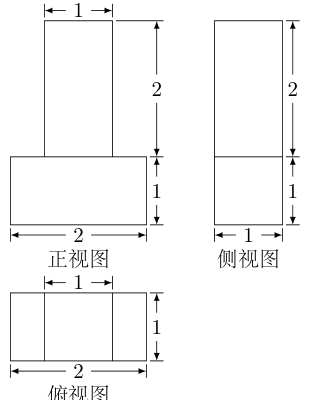
\includegraphics[width=5.5cm]{GaoKao/images/2011/tianjin_liberal/q10_fig1.png}
\end{center}

        \item 已知 \( \{a_{n}\} \) 为等差数列，\( S_{n} \) 为其前 \(n\) 项和. \( n \in \mathbb{N}^{*} \). 若 \( a_{3} = 16 \)，\( S_{20} = 20 \)，则 \(S_{10}\) 的值为\rule[-0.3ex]{3em}{0.4pt}.

        \item 已知 \(\log_2 a + \log_2 b \geqslant 1\)，则 \(3^a + 9^b\) 的最小值为\rule[-0.3ex]{3em}{0.4pt}.

        \item 如图，已知圆中两条弦 \(AB\) 与 \(CD\) 相交于点 \(F\)，\(E\) 是 \(AB\) 延长线上一点，且 \(DF = CF = \sqrt{2}\)，\(AF:FB:BE = 4:2:1\). 若 \(CE\) 与圆相切，则 \(CE\) 的长为\rule[-0.3ex]{3em}{0.4pt}.

\begin{center}
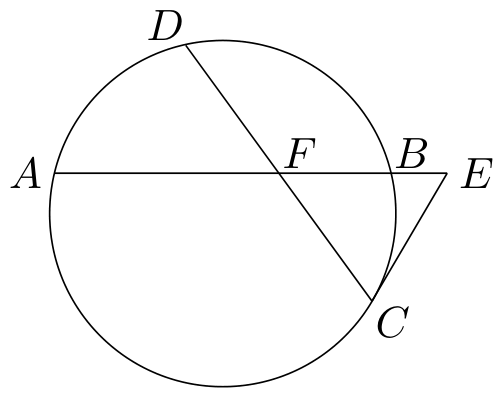
\includegraphics[width=6.0cm]{GaoKao/images/2011/tianjin_liberal/q13_fig1.png}
\end{center}

        \item 已知直角梯形 \(ABCD\) 中，\(AD \parallel BC\)，\(\angle ADC = 90^{\circ}\)，\(AD = 2\)，\(BC = 1\)，\(P\) 是腰 \(DC\) 上的动点，则 \(\left|\overrightarrow{PA}+3\overrightarrow{PB}\right|\) 的最小值为\rule[-0.3ex]{3em}{0.4pt}.

    \end{enumerate}

\end{description}

\begin{description}

    \item[三、解答题]

    \begin{enumerate}[leftmargin=5pt]

      \addtocounter{enumi}{+14}

        \item 编号分别为 \(A_{1}\)，\(A_{2}\)，\(\cdots\)，\(A_{16}\) 名篮球运动员在某次训练比赛中的得分记录如下：

\begin{center}
\begin{tabular}{|c|c|c|c|c|c|c|c|c|}
\hline
运动员编号 & \(A_{1}\) & \(A_{2}\) & \(A_{3}\) & \(A_{4}\) & \(A_{5}\) & \(A_{6}\) & \(A_{7}\) & \(A_{8}\) \\
\hline
得分 & 15 & 35 & 21 & 28 & 25 & 36 & 18 & 34 \\
\hline
运动员编号 & \(A_{9}\) & \(A_{10}\) & \(A_{11}\) & \(A_{12}\) & \(A_{13}\) & \(A_{14}\) & \(A_{15}\) & \(A_{16}\) \\
\hline
得分 & 17 & 26 & 25 & 33 & 22 & 12 & 31 & 38 \\
\hline
\end{tabular}
\end{center}

\begin{enumerate}
    \item 将得分在对应区间内的人数填入相应的空格；
    \begin{center}
    \begin{tabular}{|c|c|c|c|}
    \hline
    区间 & \([10,20)\) & \([20,30)\) & \([30,40]\) \\
    \hline
    人数 &\rule[-0.3ex]{3em}{0.4pt}&\rule[-0.3ex]{3em}{0.4pt}&\rule[-0.3ex]{3em}{0.4pt} \\
    \hline
    \end{tabular}
    \end{center}
    \item 从得分在区间 \([20, 30)\) 内的运动员中随机抽取 2 人，
    \begin{enumerate}
    \item 用运动员编号列出所有可能的抽取结果；
    \item 求这 2 人得分之和大于 50 的概率.
    \end{enumerate}
\end{enumerate}

        \item 在 \(\triangle ABC\) 中，内角 \(A\)，\(B\)，\(C\) 的对边分别为 \(a\)，\(b\)，\(c\)，已知 \(B = C\)，\(2b = \sqrt{3}a\).
\begin{enumerate}
\item 求 \(\cos A\) 的值；
\item \(\cos \left(2A + \frac{\pi}{4}\right)\) 的值.
\end{enumerate}

        \item 如图，在四棱锥 \(P - ABCD\) 中，底面 \(ABCD\) 为平行四边形，\(\angle ADC = 45^{\circ}\)，\(AD = AC = 1\)，\(O\) 为 \(AC\) 中点，\(PO \perp\) 平面 \(ABCD\)，\(PO = 2\)，\(M\) 为 \(PD\) 中点.
\begin{enumerate}
\item 证明： \(PB \parallel\) 平面 \(ACM\)；
\item 证明： \(AD \perp\) 平面 \(PAC\)；
\item 求直线 \(AM\) 与平面 \(ABCD\) 所成角的正切值.
\end{enumerate}

\begin{center}
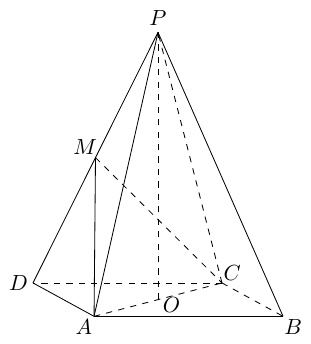
\includegraphics[width=7.7cm]{GaoKao/images/2011/tianjin_liberal/q17_fig1.png}
\end{center}

        \item 设椭圆 \(\frac{x^2}{a^{2}} + \frac{y^2}{b^{2}} = 1 \) （\(a > b > 0\)）的左、右焦点分别为 \(F_1\)，\(F_2\). 点 \(P(a, b)\) 满足 \(|PF_2| = |F_1F_2|\).
\begin{enumerate}
\item 求椭圆的离心率 \( e \)；
\item 设直线 \(PF_{2}\) 与椭圆相交于 \(A\)，\(B\) 两点，若直线 \(PF_{2}\) 与圆 \((x + 1)^{2} + (y - \sqrt{3})^{2} = 16\) 相交于 \(M\)，\(N\) 两点，且 \(|MN| = \frac{5}{8} |AB|\)，求椭圆的方程.
\end{enumerate}

        \item 已知函数 \(f(x) = 4x^{3} + 3tx^{2} - 6t^{2}x + t - 1\)，\(x \in \mathbb{R}\)，其中 \( t \in \mathbb{R}\).
\begin{enumerate}
\item 当 \(t = 1\) 时，求曲线 \(y = f(x)\) 在点 \((0, f(0))\) 处的切线方程；
\item 当 \(t \neq 0\) 时，求 \(f(x)\) 的单调区间；
\item 证明：对任意的 \(t \in (0, +\infty)\)，\(f(x)\) 在区间 \((0, 1)\) 内均存在零点.
\end{enumerate}

        \item 已知数列 \(\{a_{n}\}\) 与 \(\{b_{n}\}\) 满足： \(b_{n+1}a_{n} + b_{n}a_{n+1} = (-2)^{n} + 1\)，\(b_{n} = \frac{3 + (-1)^{n-1}}{2}\)，\(n \in \mathbb{N}^{*}\)，且 \(a_{1} = 2\).
\begin{enumerate}
\item 求 \(a_{2}\)，\(a_{3}\) 的值；
\item 设 \(c_{n} = a_{2n + 1} - a_{2n - 1}\)，\(n \in \mathbb{N}^{*}\)，证明：数列 \(\{c_{n}\}\) 是等比数列；
\item 设 \(S_{n}\) 为 \(\{a_{n}\}\) 的前 \(n\) 项和，证明 \(\frac{S_{1}}{a_{1}} + \frac{S_{2}}{a_{2}} + \ldots + \frac{S_{2n-1}}{a_{2n-1}} + \frac{S_{2n}}{a_{2n}} \leqslant n - \frac{1}{3}\) （\(n \in \mathbb{N}^{*}\)）.
\end{enumerate}

    \end{enumerate}

\end{description}


\subsection{2011年浙江卷（理）}\label{gk:2011年浙江卷（理）}

\begin{description}

    \item[一、选择题]

    \begin{enumerate}[leftmargin=5pt]

        \item 设函数 \( f(x) = \begin{cases}
-x, & x \leqslant 0,\\
x^2, & x > 0
\end{cases} \) 若 \( f(\alpha) = 4 \)，则实数 \( \alpha = \)（\quad）

        {\centering\begin{tabular*}{\linewidth}{@{}@{\extracolsep{\fill}}llll@{}}
          \text{A. }\(-4\) 或 \(-2\)  &  \text{B. }\(-4\) 或 2  &  \text{C. }\(-2\) 或 4  &  \text{D. }\(-2\) 或 2
        \end{tabular*}\par}

        \item 把复数 \(z\) 的共轭复数记作 \(\overline{z}\)，\(i\) 为虚数单位，若 \(z = 1 + \i\)，则 \((1 + z)\cdot \overline{z} =\)（\quad）

        {\centering\begin{tabular*}{\linewidth}{@{}@{\extracolsep{\fill}}llll@{}}
          \text{A. }\(3 - \i\)  &  \text{B. }\( 3 + \i \)  &  \text{C. }\( 1 + 3\i \)  &  \text{D. }\(3\)
        \end{tabular*}\par}

        \item 若某几何体的三视图如图所示，则这个几何体的直观图可以是（\quad）

\begin{center}
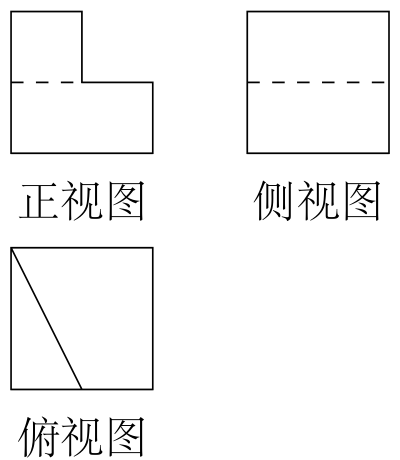
\includegraphics[width=3.9cm]{GaoKao/images/2011/zhejiang_science/q3_fig1.png}
\end{center}

        {\centering\begin{tabular*}{\linewidth}{@{}@{\extracolsep{\fill}}cccc@{}}
          \text{A. }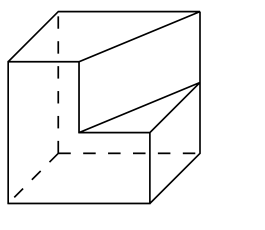
\includegraphics[width=0.15\paperwidth]{GaoKao/images/2011/zhejiang_science/q3_optA.png}  &  \text{B. }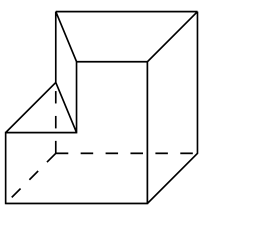
\includegraphics[width=0.15\paperwidth]{GaoKao/images/2011/zhejiang_science/q3_optB.png}  &  \text{C. }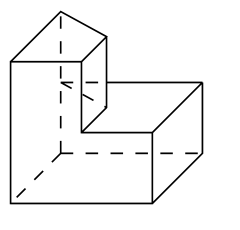
\includegraphics[width=0.15\paperwidth]{GaoKao/images/2011/zhejiang_science/q3_optC.png}  &  \text{D. }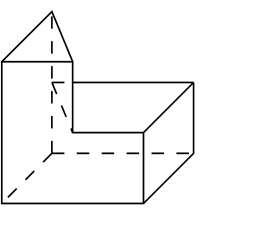
\includegraphics[width=0.15\paperwidth]{GaoKao/images/2011/zhejiang_science/q3_optD.png}
        \end{tabular*}\par}

        \item 下列命题中错误的是（\quad）

        {\centering\begin{tabular*}{\linewidth}{@{}@{\extracolsep{\fill}}llll@{}}
          \text{A. }如果平面 \(\alpha \perp\) 平面 \(\beta\)，那么平面 \(\alpha\) 内一定存在直线平行于平面 \(\beta\)  &  \text{B. }如果平面 \( \alpha \) 不垂直于平面 \( \beta \)，那么平面 \( \alpha \) 内一定不存在直线垂直于平面 \( \beta \)  &  \text{C. }如果平面 \(\alpha \perp\) 平面 \(\gamma\)，平面 \(\beta \perp\) 平面 \(\gamma\)，\(\alpha \cap \beta = l\)，那么 \(l \perp\) 平面 \(\gamma\)  &  \text{D. }如果平面 \(\alpha \perp\) 平面 \(\beta\)，那么平面 \(\alpha\) 内所有直线都垂直于平面 \(\beta\)
        \end{tabular*}\par}

        \item 设实数 \(x\)，\(y\) 满足不等式组 \(\begin{cases}
x + 2y - 5 > 0,\\
2x + y - 7 > 0,\\
x \geqslant 0, y \geqslant 0.
\end{cases}\) 若 \(x\)，\(y\) 为整数，则 \(3x + 4y\) 的最小值是（\quad）

        {\centering\begin{tabular*}{\linewidth}{@{}@{\extracolsep{\fill}}llll@{}}
          \text{A. }14  &  \text{B. }16  &  \text{C. }17  &  \text{D. }19
        \end{tabular*}\par}

        \item 若 \(0 < \alpha < \frac{\pi}{2}\)，\(-\frac{\pi}{2} < \beta < 0\)，\(\cos \left(\frac{\pi}{4} + \alpha\right) = \frac{1}{3}\)，\(\cos \left(\frac{\pi}{4} - \frac{\beta}{2}\right) = \frac{\sqrt{3}}{3}\)，则 \(\cos \left(\alpha + \frac{\beta}{2}\right) =\)（\quad）

        {\centering\begin{tabular*}{\linewidth}{@{}@{\extracolsep{\fill}}llll@{}}
          \text{A. }\(\frac{\sqrt{3}}{3}\)  &  \text{B. }\(-\frac{\sqrt{3}}{3}\)  &  \text{C. }\(\frac{5\sqrt{3}}{9}\)  &  \text{D. }\(-\frac{\sqrt{6}}{9}\)
        \end{tabular*}\par}

        \item 若 \(a\)，\(b\) 为实数，则 \(0 < ab < 1\) 是“\(a < \frac{1}{b}\) 或 \(b > \frac{1}{a}\)”的（\quad）

        {\centering\begin{tabular*}{\linewidth}{@{}@{\extracolsep{\fill}}llll@{}}
          \text{A. }充分而不必要条件  &  \text{B. }必要而不充分条件  &  \text{C. }充分必要条件  &  \text{D. }既不充分也不必要条件
        \end{tabular*}\par}

        \item 已知椭圆 \(C_{1}: \frac{x^{2}}{a^{2}} + \frac{y^{2}}{b^{2}} = 1\) （\(a > b > 0\)）与双曲线 \(C_2:  x^{2} - \frac{y^{2}}{4} = 1\) 有公共的焦点，\(C_2\) 的一条渐近线与以 \(C_1\) 的长轴为直径的圆相交于 \(A\)，\(B\) 两点. 若 \(C_1\) 恰好将线段 \(AB\) 三等分，则（\quad）

        {\centering\begin{tabular*}{\linewidth}{@{}@{\extracolsep{\fill}}llll@{}}
          \text{A. }\(a^2 = \frac{13}{2}\)  &  \text{B. }\(a^2 = 13\)  &  \text{C. }\(b^{2} = \frac{1}{2}\)  &  \text{D. }\(b^{2} = 2\)
        \end{tabular*}\par}

        \item 有 5 本不同的书，其中语文书 2 本，数学书 2 本，物理书 1 本. 若将其随机地抽取并摆放在书架的同一层上，则同一科目的书都不相邻的概率为（\quad）

        {\centering\begin{tabular*}{\linewidth}{@{}@{\extracolsep{\fill}}llll@{}}
          \text{A. }\(\frac{1}{5}\)  &  \text{B. }\(\frac{2}{5}\)  &  \text{C. }\(\frac{3}{5}\)  &  \text{D. }\(\frac{4}{5}\)
        \end{tabular*}\par}

        \item 设 \(a\)，\(b\)，\(c\) 为实数，\(f(x) = (x + a)(x^2 + bx + c)\)，\(g(x) = (ax + 1)(cx^2 + bx + 1)\). 记集合 \(S = \{x \mid f(x) = 0, x \in \mathbb{R}\}\)，\(T = \{x \mid g(x) = 0, x \in \mathbb{R}\}\)，若 \(|S|\)，\(|T|\) 分别为集合 \(S\)，\(T\) 的元素个数，则下列结论不可能的是（\quad）

        {\centering\begin{tabular*}{\linewidth}{@{}@{\extracolsep{\fill}}llll@{}}
          \text{A. }\( |S| = 1 \) 且 \( |T| = 0 \)  &  \text{B. }\( |S| = 1 \) 且 \( |T| = 1 \)  &  \text{C. }\( |S| = 2 \) 且 \( |T| = 2 \)  &  \text{D. }\( |S| = 2 \) 且 \( |T| = 3 \)
        \end{tabular*}\par}

    \end{enumerate}

\end{description}

\begin{description}

    \item[二、填空题]

    \begin{enumerate}[leftmargin=5pt]

      \addtocounter{enumi}{+10}

        \item 若函数 \( f(x) = x^2 - |x + a| \) 为偶函数，则实数 \( a = \)\rule[-0.3ex]{3em}{0.4pt}.

        \item 某程序框图如图所示，则该程序运行后输出的 \(k\) 的值是\rule[-0.3ex]{3em}{0.4pt}.

\begin{center}
\begin{center}
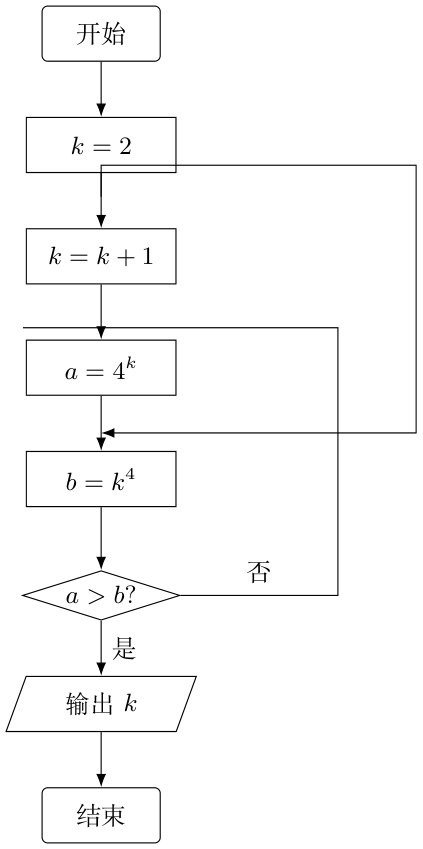
\includegraphics[width=0.70\linewidth]{GaoKao/images/2011/zhejiang_science/q12_fig1.png}
\end{center}
\end{center}

        \item 设二项式 \(\left(x - \frac{a}{\sqrt{x}}\right)^6\) （\(a > 0\)）的展开式中 \(x^3\) 的系数为 \(A\)，常数项为 \(B\). 若 \(B = 4A\)，则 \(a\) 的值是\rule[-0.3ex]{3em}{0.4pt}.

        \item 若平面向量 \(\alpha\)，\(\beta\) 满足 \(|\alpha| = 1\)，\(|\beta| \leqslant 1\)，且以向量 \(\alpha\)，\(\beta\) 为邻边的平行四边形的面积为 \(\frac{1}{2}\)，则 \(\alpha\) 和 \(\beta\) 的夹角 \(\theta\) 的取值范围是\rule[-0.3ex]{3em}{0.4pt}.

        \item 某毕业生参加人才招聘会，分别向甲，乙，丙三个公司投递了个人简历，假定该毕业生得到甲公司面试的概率为 \(\frac{2}{3}\)，得到乙，丙公司面试的概率均为 \(p\)，且三个公司是否让其面试是相互独立的. 记 \(X\) 为该毕业生得到面试的公司个数. 若 \(P(X = 0) = \frac{1}{12}\)，则随机变量 \(X\) 的数学期望 \(E(X) =\rule[-0.3ex]{3em}{0.4pt}\).

        \item 设 \(x\)，\(y\) 为实数. 若 \(4x^{2} + y^{2} + xy = 1\)，则 \(2x + y\) 的最大值是\rule[-0.3ex]{3em}{0.4pt}.

        \item 设 \(F_{1}\)，\(F_{2}\) 分别为椭圆 \(\frac{x^{2}}{3} + y^{2} = 1\) 的焦点，点 \(A\)，\(B\) 在椭圆上. 若 \(\overrightarrow{F_{1}A} = 5\overrightarrow{F_{2}B}\)，则点 \(A\) 的坐标是\rule[-0.3ex]{3em}{0.4pt}.

    \end{enumerate}

\end{description}

\begin{description}

    \item[三、解答题]

    \begin{enumerate}[leftmargin=5pt]

      \addtocounter{enumi}{+17}

        \item 在 \(\triangle ABC\) 中，角 \(A\)，\(B\)，\(C\) 所对的边分别为 \(a\)，\(b\)，\(c\). 已知 \(\sin A + \sin C = p \sin B\) （\(p \in \mathbb{R}\)），且 \(ac = \frac{1}{4} b^2\).
\begin{enumerate}
\item 当 \(p = \frac{5}{4}\)，\(b = 1\) 时，求 \(a\)，\(c\) 的值；
\item 若角 \(B\) 为锐角，求 \(p\) 的取值范围.
\end{enumerate}

        \item 已知公差不为 \(0\) 的等差数列 \(\{a_{n}\}\) 的首项 \(a_{1}\) 为 \(a\) （\(a\in\mathbb{R}\)）. 设数列的前 \(n\) 项和为 \(S_{n}\)，且 \(\frac{1}{a_{1}}\)，\(\frac{1}{a_{2}}\)，\(\frac{1}{a_{4}}\) 成等比数列.
\begin{enumerate}
\item 求数列 \( \{a_{n}\} \) 的通项公式及 \( S_{n} \)；
\item 记 \(A_{n} = \frac{1}{S_{1}} + \frac{1}{S_{2}} + \frac{1}{S_{3}} + \cdots + \frac{1}{S_{n}}\)，\(B_{n} = \frac{1}{a_{1}} + \frac{1}{a_{2}} + \frac{1}{a_{2^{2}}} + \cdots + \frac{1}{a_{2^{n-1}}}\) 当 \(n \geqslant 2\) 时，试比较 \(A_{n}\) 与 \(B_{n}\) 的大小.
\end{enumerate}

        \item 如图，在三棱锥 \(P - ABC\) 中，\(AB = AC\)，\(D\) 为 \(BC\) 的中点，\(PO \perp\) 平面 \(ABC\)，垂足 \(O\) 落在线段 \(AD\) 上，已知 \(BC = 8\)，\(PO = 4\)，\(AO = 3\)，\(OD = 2\).
\begin{enumerate}
\item 证明： \(AP \perp BC\)；
\item 在线段 \(AP\) 上是否存在点 \(M\)，使得二面角 \(A - MC - B\) 为直二面角. 若存在，求出 \(AM\) 的长；若不存在，请说明理由.
\end{enumerate}

\begin{center}
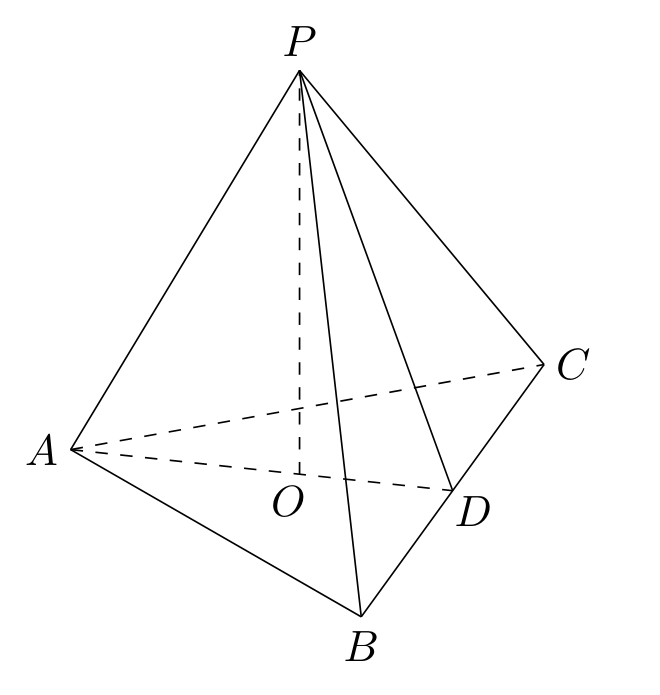
\includegraphics[width=7.0cm]{GaoKao/images/2011/zhejiang_science/q20_fig1.png}
\end{center}

        \item 已知抛物线 \(C_1: x^2 = y\)，圆 \(C_2: x^2 + (y - 4)^2 = 1\) 的圆心为点 \(M\).
\begin{enumerate}
\item 求点 \(M\) 到抛物线 \(C_{1}\) 的准线的距离；
\item 已知点 \(P\) 是抛物线 \(C_{1}\) 上一点 （异于原点），过点 \(P\) 作圆 \(C_{2}\) 的两条切线，交抛物线 \(C_{1}\) 于 \(A\)，\(B\) 两点，若过 \(M\)，\(P\) 两点的直线 \(l\) 垂直于 \(AB\)，求直线 \(l\) 的方程.
\end{enumerate}

\begin{center}
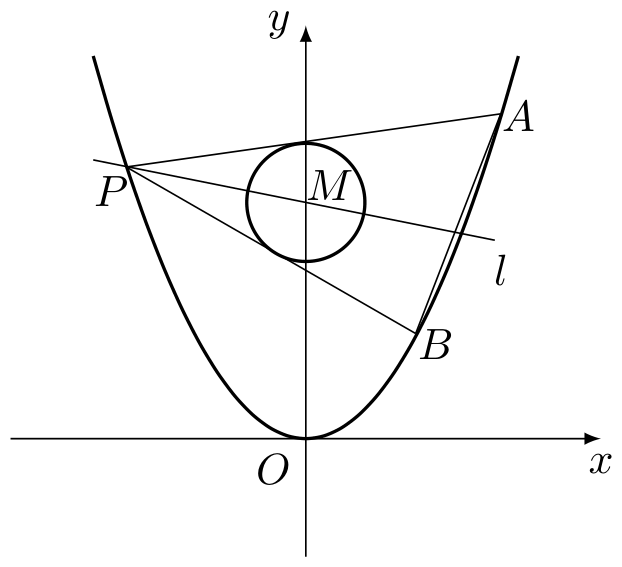
\includegraphics[width=7.2cm]{GaoKao/images/2011/zhejiang_science/q21_fig1.png}
\end{center}

        \item 设函数 \(f(x) = (x - a)^2 \ln x\)，\(a \in \mathbb{R}\).
\begin{enumerate}
\item 若 \(x = {\mathrm{e}}\) 为 \(y = f(x)\) 的极值点，求实数 \(a\)；
\item 求实数 \(a\) 的取值范围，使得对任意的 \(x \in (0,3{\mathrm{e}}]\)，恒有 \(f(x) \leqslant 4{\mathrm{e}}^2\) 成立. 注：\({\mathrm{e}}\) 为自然对数的底数.
\end{enumerate}

    \end{enumerate}

\end{description}


\subsection{2011年浙江卷（文）}\label{gk:2011年浙江卷（文）}

\begin{description}

    \item[一、选择题]

    \begin{enumerate}[leftmargin=5pt]

        \item 若 \(P = \{x \mid x < 1\}\)，\(Q = \{x \mid x > -1\}\)，则（\quad）

        {\centering\begin{tabular*}{\linewidth}{@{}@{\extracolsep{\fill}}llll@{}}
          \text{A. }\(P \subseteq Q\)  &  \text{B. }\(Q \subseteq P\)  &  \text{C. }\(\complement_{\mathbb{R}} P\subseteq Q\)  &  \text{D. }\(Q \subseteq \complement_{\mathbb{R}} P\)
        \end{tabular*}\par}

        \item 若复数 \(z = 1 + \i\)，\(\i\) 为虚数单位，则 \((1 + z)\cdot z =\)（\quad）

        {\centering\begin{tabular*}{\linewidth}{@{}@{\extracolsep{\fill}}llll@{}}
          \text{A. }\(1 + 3\i\)  &  \text{B. }\(3 + 3\i\)  &  \text{C. }\(3 - \i\)  &  \text{D. }\(3\)
        \end{tabular*}\par}

        \item 若实数 \(x\)，\(y\) 满足不等式组 \(\begin{cases}
x + 2y - 5 \geqslant 0,\\
2x + y - 7 \geqslant 0,\\
x \geqslant 0,\\
y \geqslant 0,
\end{cases}\) 则 \(3x + 4y\) 的最小值是（\quad）

        {\centering\begin{tabular*}{\linewidth}{@{}@{\extracolsep{\fill}}llll@{}}
          \text{A. }\(13\)  &  \text{B. }\(15\)  &  \text{C. }\(20\)  &  \text{D. }\(28\)
        \end{tabular*}\par}

        \item 若直线 \(l\) 不平行于平面 \(\alpha\)，且 \(l \not\subset \alpha\)，则（\quad）

        {\centering\begin{tabular*}{\linewidth}{@{}@{\extracolsep{\fill}}llll@{}}
          \text{A. }\(\alpha\) 内的所有直线与 \(l\) 异面  &  \text{B. }\(\alpha\) 内不存在与 \(l\) 平行的直线  &  \text{C. }\(\alpha\) 内存在唯一的直线与 \(l\) 平行  &  \text{D. }\(\alpha\) 内的直线与 \(l\) 都相交
        \end{tabular*}\par}

        \item 在 \(\triangle ABC\) 中，角 \(A\)，\(B\)，\(C\) 所对的边分别为 \(a\)，\(b\)，\(c\). 若 \(a \cos A = b \sin B\)，则 \(\sin A \cos A + \cos^2 B =\)（\quad）

        {\centering\begin{tabular*}{\linewidth}{@{}@{\extracolsep{\fill}}llll@{}}
          \text{A. }\(-\frac{1}{2}\)  &  \text{B. }\(\frac{1}{2}\)  &  \text{C. }\(-1\)  &  \text{D. }\(1\)
        \end{tabular*}\par}

        \item 若 \(a\)，\(b\) 为实数，则“\(0 < ab < 1\)”是“\(b < \frac{1}{a}\)”的（\quad）

        {\centering\begin{tabular*}{\linewidth}{@{}@{\extracolsep{\fill}}llll@{}}
          \text{A. }充分而不必要条件  &  \text{B. }必要而不充分条件  &  \text{C. }充分必要条件  &  \text{D. }既不充分也不必要条件
        \end{tabular*}\par}

        \item 若某几何体的三视图如图所示，则这个几何体的直观图可以是（\quad）

\begin{center}
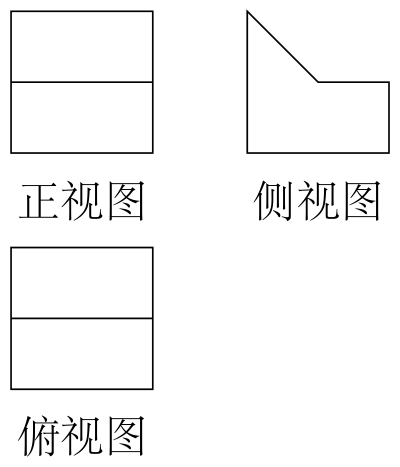
\includegraphics[width=3.9cm]{GaoKao/images/2011/zhejiang_liberal/q7_fig1.png}
\end{center}

        {\centering\begin{tabular*}{\linewidth}{@{}@{\extracolsep{\fill}}cccc@{}}
          \text{A. }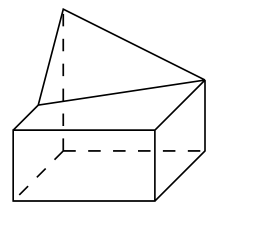
\includegraphics[width=0.15\paperwidth]{GaoKao/images/2011/zhejiang_liberal/q7_optA.png}  &  \text{B. }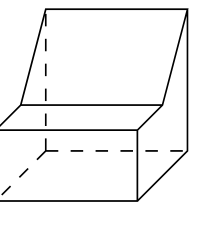
\includegraphics[width=0.15\paperwidth]{GaoKao/images/2011/zhejiang_liberal/q7_optB.png}  &  \text{C. }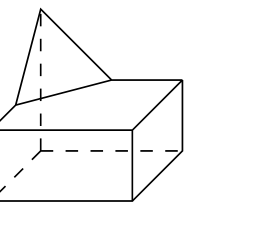
\includegraphics[width=0.15\paperwidth]{GaoKao/images/2011/zhejiang_liberal/q7_optC.png}  &  \text{D. }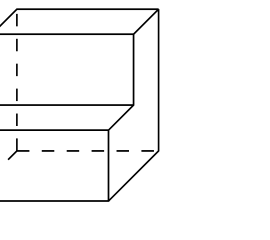
\includegraphics[width=0.15\paperwidth]{GaoKao/images/2011/zhejiang_liberal/q7_optD.png}
        \end{tabular*}\par}

        \item 从装有 3 个红球，2 个白球的袋中任取 3 个球，则所取的 3 个球中至少有 1 个白球的概率是（\quad）

        {\centering\begin{tabular*}{\linewidth}{@{}@{\extracolsep{\fill}}llll@{}}
          \text{A. }\( \frac{1}{10} \)  &  \text{B. }\( \frac{3}{10} \)  &  \text{C. }\( \frac{3}{5} \)  &  \text{D. }\( \frac{9}{10} \)
        \end{tabular*}\par}

        \item 已知椭圆 \(C_{1}: \frac{x^{2}}{a^{2}} + \frac{y^{2}}{b^{2}} = 1\) （\(a>b>0\)） 与双曲线 \(C_2: x^{2} - \frac{y^{2}}{4} = 1\) 有公共的焦点， \(C_2\) 的一条渐近线与以 \(C_1\) 的长轴为直径的圆相交于 \(A\)，\(B\) 两点. 若 \(C_1\) 恰好将线段 \(AB\) 三等分，则（\quad）

        {\centering\begin{tabular*}{\linewidth}{@{}@{\extracolsep{\fill}}llll@{}}
          \text{A. }\(a^2 = \frac{13}{2}\)  &  \text{B. }\(a^2 = 13\)  &  \text{C. }\(b^{2} = \frac{1}{2}\)  &  \text{D. }\(b^{2} = 2\)
        \end{tabular*}\par}

        \item 设函数 \( f(x) = ax^2 + bx + c \)，（\(a\)，\(b\)，\(c\in\mathbb{R}\)）. 若 \(x = -1\) 为函数 \( y = f(x){\mathrm{e}}^x \) 的一个极值点，则下列图象不可能为 \( y = f(x) \) 图象的是（\quad）

        {\centering\begin{tabular*}{\linewidth}{@{}@{\extracolsep{\fill}}cccc@{}}
          \text{A. }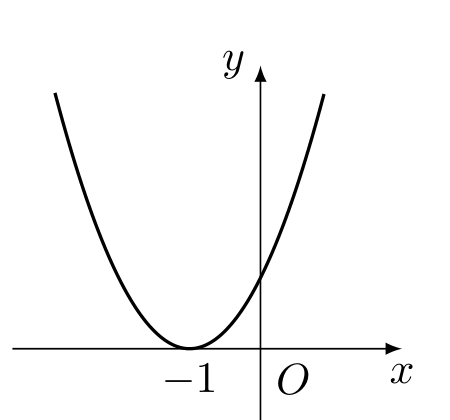
\includegraphics[width=0.15\paperwidth]{GaoKao/images/2011/zhejiang_liberal/q10_optA.png}  &  \text{B. }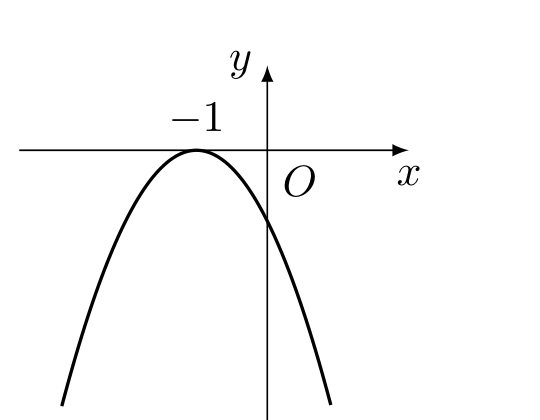
\includegraphics[width=0.15\paperwidth]{GaoKao/images/2011/zhejiang_liberal/q10_optB.png}  &  \text{C. }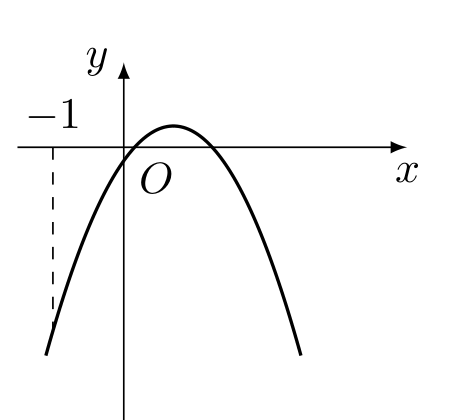
\includegraphics[width=0.15\paperwidth]{GaoKao/images/2011/zhejiang_liberal/q10_optC.png}  &  \text{D. }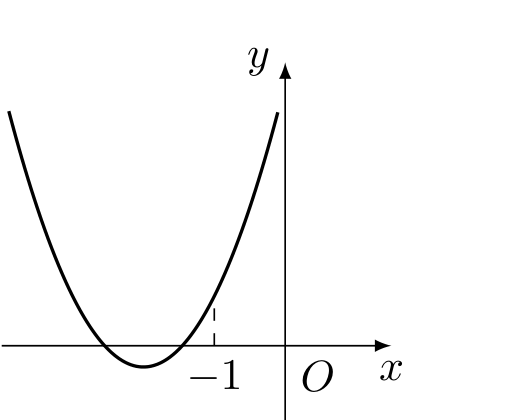
\includegraphics[width=0.15\paperwidth]{GaoKao/images/2011/zhejiang_liberal/q10_optD.png}
        \end{tabular*}\par}

    \end{enumerate}

\end{description}

\begin{description}

    \item[二、填空题]

    \begin{enumerate}[leftmargin=5pt]

      \addtocounter{enumi}{+10}

        \item 设函数 \( f(x) = \frac{4}{1 - x} \). 若 \( f(a) = 2 \)，则实数 \( a = \)\rule[-0.3ex]{3em}{0.4pt}.

        \item 若直线 \(x - 2y + 5 = 0\) 与直线 \(2x + my - 6 = 0\) 互相垂直，则实数 \(m = \)\rule[-0.3ex]{3em}{0.4pt}.

        \item 某小学为了解学生数学课程的学习情况，在 \(3000\) 名学生中随机抽取 \(200\) 名，并统计这 \(200\) 名学生的某次数学考试成绩，得到了样本的频率分布直方图（如图）. 根据频率分布直方图，\(3000\) 名学生在该次数学考试中成绩小于 \(60\) 分的学生数是\rule[-0.3ex]{3em}{0.4pt}.
\begin{center}
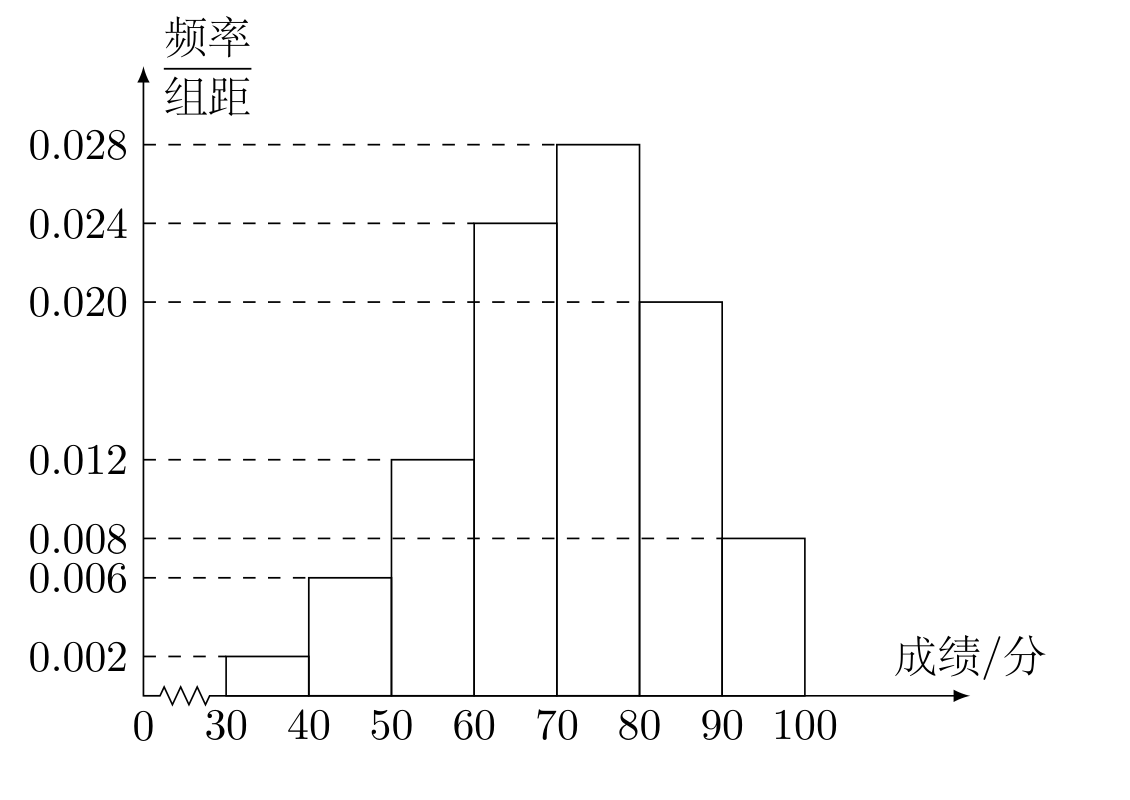
\includegraphics[width=0.42\linewidth]{GaoKao/images/2011/zhejiang_liberal/q13_fig1.png}
\end{center}

        \item 某程序框图如图所示，则该程序运行后输出的 \(k\) 的值是\rule[-0.3ex]{3em}{0.4pt}.
\begin{center}
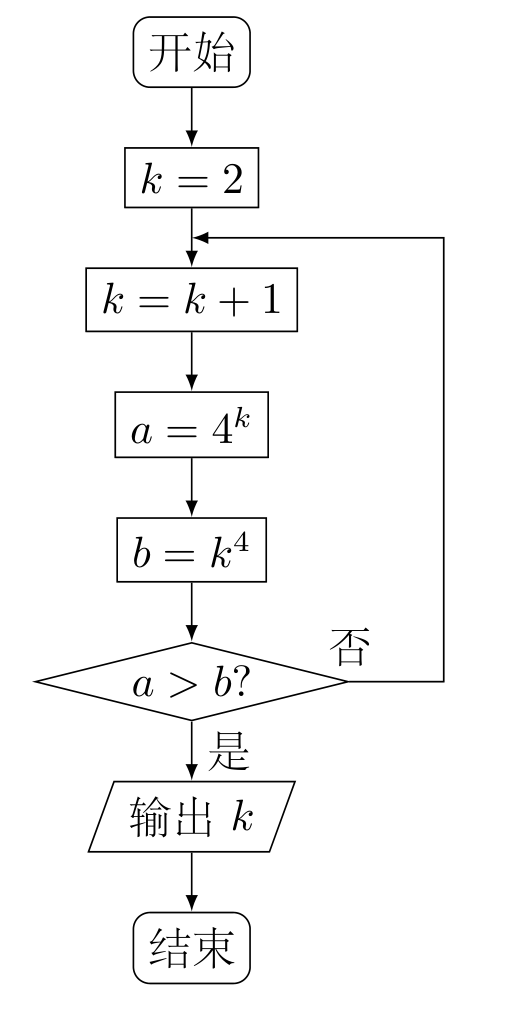
\includegraphics[width=0.70\linewidth]{GaoKao/images/2011/zhejiang_liberal/q14_fig1.png}
\end{center}

        \item 若平面向量 \(\bm{\alpha}\)，\(\bm{\beta}\) 满足 \(|\bm{\alpha}| = 1\)，\(|\bm{\beta}| \leqslant 1\)，且以向量 \(\bm{\alpha}\)，\(\bm{\beta}\) 为邻边的平行四边形的面积为 \(\frac{1}{2}\)，则 \(\bm{\alpha}\) 和 \(\bm{\beta}\) 的夹角 \(\theta\) 的取值范围是\rule[-0.3ex]{3em}{0.4pt}.

        \item 若实数 \(x\)，\(y\) 满足 \(x^{2} + y^{2} + xy = 1\)，则 \(x + y\) 的最大值是\rule[-0.3ex]{3em}{0.4pt}.

        \item 若数列 \(\left\{n(n + 4)\left(\frac{2}{3}\right)^n\right\}\) 中的最大项是第 \(k\) 项，则 \(k = \)\rule[-0.3ex]{3em}{0.4pt}.

    \end{enumerate}

\end{description}

\begin{description}

    \item[三、解答题]

    \begin{enumerate}[leftmargin=5pt]

      \addtocounter{enumi}{+17}

        \item 已知函数 \( f(x) = A \sin \left( \frac{\pi}{3} x + \varphi \right) \)，\( x \in \mathbb{R} \)，\(A > 0\)，\(0 < \varphi < \frac{\pi}{2}\). \( y = f(x) \) 的部分图象如图所示，\(P\)，\(Q\) 分别为该图象的最高点和最低点，点 \(P\) 的坐标为 \((1,A)\).

\begin{enumerate}
\item 求 \( f(x) \) 的最小正周期及 \( \varphi \) 的值；
\item 若点 \(R\) 的坐标为 \((1,0)\)，\(\angle PRQ = \frac{2\pi}{3}\)，求 \(A\) 的值.
\end{enumerate}

\begin{center}
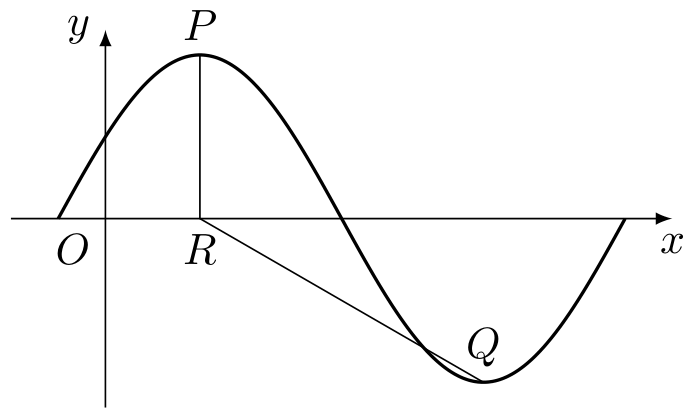
\includegraphics[width=4.0cm]{GaoKao/images/2011/zhejiang_liberal/q18_fig1.png}
\end{center}

        \item 已知公差不为 0 的等差数列 \(\{a_{n}\}\) 的首项 \(a_{1}\) 为 \(a\) （\(a \in \mathbb{R}\)），且 \(\frac{1}{a_1}\)，\(\frac{1}{a_2}\)，\(\frac{1}{a_4}\) 成等比数列.
\begin{enumerate}
\item 求数列 \( \{a_{n}\} \) 的通项公式；
\item 对 \(n \in \mathbb{N}^*\)，试比较 \(\frac{1}{a_2} + \frac{1}{a_{2^2}} + \frac{1}{a_{2^3}} + \cdots + \frac{1}{a_{2^n}}\) 与 \(\frac{1}{a_1}\) 的大小.
\end{enumerate}

        \item 如图，在三棱锥 \(P - ABC\) 中，\(AB = AC\)，\(D\) 为 \(BC\) 的中点，\(PO \perp\) 平面 \(ABC\)，垂足 \(O\) 落在线段 \(AD\) 上.
\begin{enumerate}
\item 证明： \(AP \perp BC\)；
\item 已知 \(BC = 8\)，\(PO = 4\)，\(AO = 3\)，\(OD = 2\). 求二面角 \(B - AP - C\) 的大小.
\end{enumerate}
\begin{center}
\includegraphics[width=7.7cm]{GaoKao/images/2011/zhejiang_liberal/q20_fig1.png}
\end{center}

        \item 设函数 \(f(x) = a^2 \ln x - x^2 + ax\)，\(a > 0\).
\begin{enumerate}
\item 求 \( f(x) \) 的单调区间；
\item 求所有实数 \(a\)，使 \({\mathrm{e}} - 1 \leqslant f(x) \leqslant {\mathrm{e}}^{2}\) 对 \(x \in [1, {\mathrm{e}}]\) 恒成立. 注：\({\mathrm{e}}\) 为自然对数的底数.
\end{enumerate}

        \item 如图，设 \(P\) 为抛物线 \(C_1: x^2 = y\) 上的动点，过点 \(P\) 做圆 \(C_2: x^2 + (y + 3)^2 = 1\) 的两条切线，交直线 \(l: y = -3\) 于 \(A\)，\(B\) 两点.
\begin{enumerate}
\item 求 \(C_{2}\) 的圆心 \(M\) 到抛物线 \(C_{1}\) 准线的距离.
\item 是否存在点 \(P\)，使线段 \(AB\) 被抛物线 \(C_1\) 在点 \(P\) 处的切线平分，若存在，求出点 \(P\) 的坐标；若不存在，请说明理由.
\end{enumerate}
\begin{center}
\includegraphics[width=5.5cm]{GaoKao/images/2011/zhejiang_liberal/q22_fig1.png}
\end{center}

    \end{enumerate}

\end{description}

\section{2012年高考题}

\subsection{2012年大纲卷（理）}\label{gk:2012年大纲卷（理）}

\begin{description}

    \item[一、选择题]

    \begin{enumerate}[leftmargin=5pt]

        \item 复数 \(\frac{-1 + 3\i}{1 + \i} =\)（\quad）

        {\centering\begin{tabular*}{\linewidth}{@{}@{\extracolsep{\fill}}llll@{}}
          \text{A. }\(2 + \i\)  &  \text{B. }\(2 - \i\)  &  \text{C. }\(1 + 2\i\)  &  \text{D. }\(1 - 2\i\)
        \end{tabular*}\par}

        \item 已知集合 \(A = \{1, 3, \sqrt{m}\}\)，\(B = \{1, m\}\)，\(A \cup B = A\)，则 \(m =\)（\quad）

        {\centering\begin{tabular*}{\linewidth}{@{}@{\extracolsep{\fill}}llll@{}}
          \text{A. }\(0\) 或 \(\sqrt{3}\)  &  \text{B. }\(0\) 或 \(3\)  &  \text{C. }\(1\) 或 \(\sqrt{3}\)  &  \text{D. }\(1\) 或 \(3\)
        \end{tabular*}\par}

        \item 椭圆的中心在原点，焦距为 \(4\)，一条准线为 \(x = -4\)，则该椭圆的方程为（\quad）

        {\centering\begin{tabular*}{\linewidth}{@{}@{\extracolsep{\fill}}llll@{}}
          \text{A. }\(\frac{x^2}{16} + \frac{y^2}{12} = 1\)  &  \text{B. }\(\frac{x^2}{12} + \frac{y^2}{8} = 1\)  &  \text{C. }\(\frac{x^2}{8} + \frac{y^2}{4} = 1\)  &  \text{D. }\(\frac{x^2}{12} + \frac{y^2}{4} = 1\)
        \end{tabular*}\par}

        \item 已知正四棱柱 \(ABCD - A_{1}B_{1}C_{1}D_{1}\) 中，\(AB = 2\)，\(CC_{1} = 2\sqrt{2}\)，\(E\) 为 \(CC_{1}\) 的中点，则直线 \(AC_{1}\) 到平面 \(BED\) 的距离为（\quad）

        {\centering\begin{tabular*}{\linewidth}{@{}@{\extracolsep{\fill}}llll@{}}
          \text{A. }\(2\)  &  \text{B. }\(\sqrt{3}\)  &  \text{C. }\(\sqrt{2}\)  &  \text{D. }\(1\)
        \end{tabular*}\par}

        \item 已知等差数列 \(\{a_{n}\}\) 前 \(n\) 项和为 \(S_{n}\). \(a_{5} = 5\)，\(S_{5} = 15\)，则数列 \(\left\{\frac{1}{a_n a_{n+1}}\right\}\) 的前 \(100\) 项和为（\quad）

        {\centering\begin{tabular*}{\linewidth}{@{}@{\extracolsep{\fill}}llll@{}}
          \text{A. }\(\frac{100}{101}\)  &  \text{B. }\(\frac{99}{101}\)  &  \text{C. }\(\frac{99}{100}\)  &  \text{D. }\(\frac{101}{100}\)
        \end{tabular*}\par}

        \item \(\triangle ABC\) 中，\(AB\) 边的高为 \(CD\)，若 \(\overrightarrow{CB} = \bm{a}\)，\(\overrightarrow{CA} = \bm{b}\)，\(\bm{a} \cdot \bm{b} = 0\)，\(|\bm{a}| = 1\)，\(|\bm{b}| = 2\)，则 \(\overrightarrow{AD} =\)（\quad）

        {\centering\begin{tabular*}{\linewidth}{@{}@{\extracolsep{\fill}}llll@{}}
          \text{A. }\(\frac{1}{3}\bm{a} - \frac{1}{3}\bm{b}\)  &  \text{B. }\(\frac{2}{3}\bm{a} - \frac{2}{3}\bm{b}\)  &  \text{C. }\(\frac{2}{3}\bm{a} - \frac{3}{5}\bm{b}\)  &  \text{D. }\(\frac{4}{5}\bm{a} - \frac{4}{5}\bm{b}\)
        \end{tabular*}\par}

        \item 已知 \(\alpha\) 为第二象限角，\(\sin \alpha + \cos \alpha = \frac{\sqrt{3}}{3}\)，则 \(\cos 2\alpha =\)（\quad）

        {\centering\begin{tabular*}{\linewidth}{@{}@{\extracolsep{\fill}}llll@{}}
          \text{A. }\(-\frac{\sqrt{5}}{3}\)  &  \text{B. }\(-\frac{\sqrt{5}}{9}\)  &  \text{C. }\(\frac{\sqrt{5}}{9}\)  &  \text{D. }\(\frac{\sqrt{5}}{3}\)
        \end{tabular*}\par}

        \item 已知 \(F_{1}\)，\(F_{2}\) 为双曲线 \(C: x^{2} - y^{2} = 2\) 的左，右焦点，点 \(P\) 在 \(C\) 上，\(|PF_{1}| = 2|PF_{2}|\)，则 \(\cos \angle F_{1}PF_{2} =\)（\quad）

        {\centering\begin{tabular*}{\linewidth}{@{}@{\extracolsep{\fill}}llll@{}}
          \text{A. }\(\frac{1}{4}\)  &  \text{B. }\(\frac{3}{5}\)  &  \text{C. }\(\frac{3}{4}\)  &  \text{D. }\(\frac{4}{5}\)
        \end{tabular*}\par}

        \item 已知 \(x = \ln \pi\)，\(y = \log_5 2\)，\(z = {\mathrm{e}}^{-\frac{1}{2}}\)，则（\quad）

        {\centering\begin{tabular*}{\linewidth}{@{}@{\extracolsep{\fill}}llll@{}}
          \text{A. }\(x < y < z\)  &  \text{B. }\(z < x < y\)  &  \text{C. }\(z < y < x\)  &  \text{D. }\(y < z < x\)
        \end{tabular*}\par}

        \item 已知函数 \( y = x^3 - 3x + c \) 的图象与 \( x \) 轴恰有两个公共点，则 \( c = \)（\quad）

        {\centering\begin{tabular*}{\linewidth}{@{}@{\extracolsep{\fill}}llll@{}}
          \text{A. }\(-2\) 或 \(2\)  &  \text{B. }\(-9\) 或 \(3\)  &  \text{C. }\(-1\) 或 \(1\)  &  \text{D. }\(-3\) 或 \(1\)
        \end{tabular*}\par}

        \item 将字母 \(a\)，\(a\)，\(b\)，\(b\)，\(c\)，\(c\) 排成三行两列，要求每行的字母互不相同，每列的字母也互不相同，则不同的排列方法共有（\quad）

        {\centering\begin{tabular*}{\linewidth}{@{}@{\extracolsep{\fill}}llll@{}}
          \text{A. }\(12\) 种  &  \text{B. }\(18\) 种  &  \text{C. }\(24\) 种  &  \text{D. }\(36\) 种
        \end{tabular*}\par}

        \item 正方形 \(ABCD\) 的边长为 \(1\)，点 \(E\) 在边 \(AB\) 上，点 \(F\) 在边 \(BC\) 上，\(AE = BF = \frac{3}{7}\)，动点 \(P\) 从 \(E\) 出发沿直线向 \(F\) 运动，每当碰到正方形的边时反弹，反弹时反射角等于入射角，当点 \(P\) 第一次碰到 \(E\) 时，\(P\) 与正方形的边碰撞的次数为（\quad）

        {\centering\begin{tabular*}{\linewidth}{@{}@{\extracolsep{\fill}}llll@{}}
          \text{A. }\(16\)  &  \text{B. }\(14\)  &  \text{C. }\(12\)  &  \text{D. }\(10\)
        \end{tabular*}\par}

    \end{enumerate}

\end{description}

\begin{description}

    \item[二、填空题]

    \begin{enumerate}[leftmargin=5pt]

      \addtocounter{enumi}{+12}

        \item 若 \(x\)，\(y\) 满足约束条件 \(\begin{cases}
x - y + 1 \geqslant 0,\\
x + y - 3 \leqslant 0,\\
x + 3y - 3 \geqslant 0,
\end{cases}\) 则 \(z = 3x - y\) 的最小值为\rule[-0.3ex]{3em}{0.4pt}.

        \item 当函数 \(y = \sin x - \sqrt{3}\cos x\)（\(0 \leqslant x < 2\pi\)）取得最大值时，\(x =\)\rule[-0.3ex]{3em}{0.4pt}.

        \item 若 \(\left(x + \frac{1}{x}\right)^n\) 的展开式中第\(3\)项与第\(7\)项的二项式系数相等，则该展开式中 \(\frac{1}{x^2}\) 的系数为\rule[-0.3ex]{3em}{0.4pt}.

        \item 三棱柱 \(ABC - A_{1}B_{1}C_{1}\) 中，底面边长和侧棱长都相等，\(\angle BAA_{1} = \angle CAA_{1} = 60^{\circ}\)，则异面直线 \(AB_{1}\) 与 \(BC_{1}\) 所成角的余弦值为\rule[-0.3ex]{3em}{0.4pt}.

    \end{enumerate}

\end{description}

\begin{description}

    \item[三、解答题]

    \begin{enumerate}[leftmargin=5pt]

      \addtocounter{enumi}{+16}

        \item \(\triangle ABC\) 的内角 \(A\)，\(B\)，\(C\) 的对边分别为 \(a\)，\(b\)，\(c\)，已知 \(\cos (A - C) + \cos B = 1\)，\(a = 2c\)，求 \(C\).

        \item 如图，四棱锥 \(P - ABCD\) 中，底面 \(ABCD\) 为菱形，\(PA \perp\) 底面 \(ABCD\)，\(AC = 2\sqrt{2}\)，\(PA = 2\)，\(E\) 是 \(PC\) 上的一点，\(PE = 2EC\).
\begin{enumerate}
\item 证明： \(PC \perp\) 平面 \(BED\)；
\item 设二面角 \(A - PB - C\) 为 \(90^{\circ}\)，求 \(PD\) 与平面 \(PBC\) 所成角的大小.
\end{enumerate}
\begin{center}
\includegraphics[width=7.1cm]{GaoKao/images/2012/syllabus_science/q18_fig1.png}
\end{center}

        \item 乒乓球比赛规则规定：一局比赛，双方比分在\(10\)平前，一方连续发球\(2\)次后，对方再连续发球\(2\)次，依次轮换. 每次发球，胜方得\(1\)分，负方得\(0\)分. 设在甲，乙的比赛中，每次发球，发球方得\(1\)分的概率为\(0.6\)，各次发球的胜负结果相互独立. 甲，乙的一局比赛中，甲先发球.
\begin{enumerate}
\item 求开始第\(4\)次发球时，甲，乙的比分为\(1\)比\(2\)的概率；
\item \( \xi \) 表示开始第 4 次发球时乙的得分，求 \( \xi \) 的期望.
\end{enumerate}

        \item 设函数 \(f(x) = ax + \cos x\)，\(x \in [0, \pi]\)：
\begin{enumerate}
\item 讨论 \( f(x) \) 的单调性；
\item 设 \( f(x) \leqslant 1 + \sin x \)，求 \( a \) 的取值范围.
\end{enumerate}

        \item 已知抛物线 \(C: y = (x + 1)^2\) 与圆 \(M: (x - 1)^2 + \left(y - \frac{1}{2}\right)^2 = r^2 \) （\(r > 0\)）有一个公共点 \(A\)，且在 \(A\) 处两曲线的切线为同一直线 \(l\).
\begin{enumerate}
\item 求 \(r\)；
\item 设 \(m\)，\(n\) 是异于 \(l\) 且与 \(C\) 及 \(M\) 都相切的两条直线，\(m\)，\(n\) 的交点为 \(D\)，求 \(D\) 到 \(l\) 的距离.
\end{enumerate}

        \item 函数 \( f(x) = x^2 - 2x - 3 \). 定义数列 \( \{x_n\} \) 如下： \(x_1 = 2\)，\(x_{n+1}\) 是过两点 \(P(4,5)\)，\(Q_n(x_n, f(x_n))\) 的直线 \( PQ_n \) 与 \( x \) 轴交点的横坐标.
\begin{enumerate}
\item 证明： \(2 \leqslant x_{n} < x_{n+1} < 3\).
\item 求数列 \(\{x_{n}\}\) 的通项公式.
\end{enumerate}

    \end{enumerate}

\end{description}


\subsection{2012年大纲卷（文）}\label{gk:2012年大纲卷（文）}

\begin{description}

    \item[一、选择题]

    \begin{enumerate}[leftmargin=5pt]

        \item 已知集合 \(A = \{x \mid x\text{ 是平行四边形}\}\)，\(B = \{x \mid x\text{ 是矩形}\}\)，\(C = \{x \mid x\text{ 是正方形}\}\)，\(D = \{x \mid x\text{ 是菱形}\}\)，则（\quad）

        {\centering\begin{tabular*}{\linewidth}{@{}@{\extracolsep{\fill}}llll@{}}
          \text{A. }\(A \subseteq B\)  &  \text{B. }\(C \subseteq B\)  &  \text{C. }\(D \subseteq C\)  &  \text{D. }\(A \subseteq D\)
        \end{tabular*}\par}

        \item 函数 \( y = \sqrt{x + 1} \) （\(x \geqslant -1\)）的反函数为（\quad）

        {\centering\begin{tabular*}{\linewidth}{@{}@{\extracolsep{\fill}}llll@{}}
          \text{A. }\( y = x^{2} - 1 \)（\(x \geqslant 0\)）  &  \text{B. }\( y = x^{2} - 1 \)（\(x \geqslant 1\)）  &  \text{C. }\( y = x^{2} + 1 \)（\(x \geqslant 0\)）  &  \text{D. }\( y = x^{2} + 1 \)（\(x \geqslant 1\)）
        \end{tabular*}\par}

        \item 若函数 \( f(x) = \sin \frac{x + \varphi}{3} \)（\(\varphi \in [0, 2\pi]\)）是偶函数，则 \( \varphi = \)（\quad）

        {\centering\begin{tabular*}{\linewidth}{@{}@{\extracolsep{\fill}}llll@{}}
          \text{A. }\(\frac{\pi}{2}\)  &  \text{B. }\(\frac{2\pi}{3}\)  &  \text{C. }\(\frac{3\pi}{2}\)  &  \text{D. }\(\frac{5\pi}{3}\)
        \end{tabular*}\par}

        \item 已知 \(\alpha\) 为第二象限角，\(\sin \alpha = \frac{3}{5}\)，则 \(\sin 2\alpha =\)（\quad）

        {\centering\begin{tabular*}{\linewidth}{@{}@{\extracolsep{\fill}}llll@{}}
          \text{A. }\(-\frac{24}{25}\)  &  \text{B. }\(-\frac{12}{25}\)  &  \text{C. }\(\frac{12}{25}\)  &  \text{D. }\(\frac{24}{25}\)
        \end{tabular*}\par}

        \item 椭圆的中心在原点，焦距为 \(4\)，一条准线为 \(x = -4\)，则该椭圆的方程为（\quad）

        {\centering\begin{tabular*}{\linewidth}{@{}@{\extracolsep{\fill}}llll@{}}
          \text{A. }\(\frac{x^2}{16} +\frac{y^2}{12} = 1\)  &  \text{B. }\(\frac{x^2}{12} +\frac{y^2}{8} = 1\)  &  \text{C. }\(\frac{x^2}{8} +\frac{y^2}{4} = 1\)  &  \text{D. }\(\frac{x^2}{12} +\frac{y^2}{4} = 1\)
        \end{tabular*}\par}

        \item 已知数列 \(\{a_{n}\}\) 的前 \(n\) 项和为 \(S_{n}\)，\(a_{1} = 1\)，\(S_{n} = 2a_{n+1}\)，则 \(S_{n} =\)（\quad）

        {\centering\begin{tabular*}{\linewidth}{@{}@{\extracolsep{\fill}}llll@{}}
          \text{A. }\(2^{n - 1}\)  &  \text{B. }\(\left(\frac{3}{2}\right)^{n - 1}\)  &  \text{C. }\(\left(\frac{2}{3}\right)^{n - 1}\)  &  \text{D. }\(\frac{1}{2^{n - 1}}\)
        \end{tabular*}\par}

        \item \(6\) 位选手依次演讲，其中选手甲不在第一个也不在最后一个演讲，则不同的演讲次序共有（\quad）

        {\centering\begin{tabular*}{\linewidth}{@{}@{\extracolsep{\fill}}llll@{}}
          \text{A. }\(240\) 种  &  \text{B. }\(360\) 种  &  \text{C. }\(480\) 种  &  \text{D. }\(720\) 种
        \end{tabular*}\par}

        \item 已知正四棱柱 \(ABCD - A_{1}B_{1}C_{1}D_{1}\) 中，\(AB = 2\)，\(CC_{1} = 2\sqrt{2}\)，\(E\) 为 \(CC_{1}\) 的中点，则直线 \(AC_{1}\) 到平面 \(BED\) 的距离为（\quad）

        {\centering\begin{tabular*}{\linewidth}{@{}@{\extracolsep{\fill}}llll@{}}
          \text{A. }2  &  \text{B. }\(\sqrt{3}\)  &  \text{C. }\(\sqrt{2}\)  &  \text{D. }1
        \end{tabular*}\par}

        \item \(\triangle ABC\) 中，\(AB\) 边的高为 \(CD\)，若 \(\overrightarrow{CB} = \bm{a}\)，\(\overrightarrow{CA} = \bm{b}\)，\(\bm{a} \cdot \bm{b} = 0\)，\(|\bm{a}| = 1\)，\(|\bm{b}| = 2\)，则 \(\overrightarrow{AD} =\)（\quad）

        {\centering\begin{tabular*}{\linewidth}{@{}@{\extracolsep{\fill}}llll@{}}
          \text{A. }\(\frac{1}{3}\bm{a} - \frac{1}{3}\bm{b}\)  &  \text{B. }\(\frac{2}{3}\bm{a} - \frac{2}{3}\bm{b}\)  &  \text{C. }\(\frac{3}{5}\bm{a} - \frac{3}{5}\bm{b}\)  &  \text{D. }\(\frac{4}{5}\bm{a} - \frac{4}{5}\bm{b}\)
        \end{tabular*}\par}

        \item 已知 \(F_{1}\)，\(F_{2}\) 为双曲线 \(C: x^{2} - y^{2} = 2\) 的左、右焦点，点 \(P\) 在 \(C\) 上，\(|PF_{1}| = 2|PF_{2}|\)，则 \(\cos \angle F_{1}PF_{2} =\)（\quad）

        {\centering\begin{tabular*}{\linewidth}{@{}@{\extracolsep{\fill}}llll@{}}
          \text{A. }\(\frac{1}{4}\)  &  \text{B. }\(\frac{3}{5}\)  &  \text{C. }\(\frac{3}{4}\)  &  \text{D. }\(\frac{4}{5}\)
        \end{tabular*}\par}

        \item 已知 \(x = \ln \pi\)，\(y = \log_5 2\)，\(z = {\mathrm{e}}^{-\frac{1}{2}}\)，则（\quad）

        {\centering\begin{tabular*}{\linewidth}{@{}@{\extracolsep{\fill}}llll@{}}
          \text{A. }\(x < y < z\)  &  \text{B. }\(z < x < y\)  &  \text{C. }\(z < y < x\)  &  \text{D. }\(y < z < x\)
        \end{tabular*}\par}

        \item 正方形 \(ABCD\) 的边长为 \(1\)，点 \(E\) 在边 \(AB\) 上，点 \(F\) 在边 \(BC\) 上，\(AE = BF = \frac{1}{3}\). 动点 \(P\) 从 \(E\) 出发沿直线向 \(F\) 运动，每当碰到正方形的边时反弹，反弹时反射角等于入射角，当点 \(P\) 第一次碰到 \(E\) 时，\(P\) 与正方形的边碰撞的次数为（\quad）

        {\centering\begin{tabular*}{\linewidth}{@{}@{\extracolsep{\fill}}llll@{}}
          \text{A. }8  &  \text{B. }6  &  \text{C. }4  &  \text{D. }3
        \end{tabular*}\par}

    \end{enumerate}

\end{description}

\begin{description}

    \item[二、填空题]

    \begin{enumerate}[leftmargin=5pt]

      \addtocounter{enumi}{+12}

        \item \(\left(x + \frac{1}{2x}\right)^8\) 的展开式中 \(x^2\) 的系数为\rule[-0.3ex]{3em}{0.4pt}.

        \item 若 \(x\)，\(y\) 满足约束条件 \(\begin{cases}
x - y + 1 \geqslant 0,\\
x + y - 3 \leqslant 0,\\
x + 3y - 3 \geqslant 0,
\end{cases}\) 则 \(z = 3x - y\) 的最小值为\rule[-0.3ex]{3em}{0.4pt}.

        \item 当函数 \( y = \sin x - \sqrt{3}\cos x \)（\(0 \leqslant x < 2\pi\)）取得最大值时，\( x = \)\rule[-0.3ex]{3em}{0.4pt}.

        \item 已知正方体 \(ABCD - A_{1}B_{1}C_{1}D_{1}\) 中，\(E\)，\(F\) 分别为 \(BB_{1}\)，\(CC_{1}\) 的中点，那么异面直线 \(AE\) 与 \(D_{1}F\) 所成角的余弦值为\rule[-0.3ex]{3em}{0.4pt}.

    \end{enumerate}

\end{description}

\begin{description}

    \item[三、解答题]

    \begin{enumerate}[leftmargin=5pt]

      \addtocounter{enumi}{+16}

        \item \(\triangle ABC\) 的内角 \(A\)，\(B\)，\(C\) 成等差数列，其对边 \(a\)，\(b\)，\(c\) 满足 \(2b^{2} = 3ac\)，求 \(A\).

        \item 已知数列 \( \{a_{n}\} \) 中， \( a_{1}=1 \)，前 \(n\) 项和 \( S_{n}=\frac{n+2}{3}a_{n} \).
\begin{enumerate}
\item 求 \(a_{2}\)，\(a_{3}\).
\item 求 \( \{a_{n}\} \) 的通项公式.
\end{enumerate}

        \item 如图，四棱锥 \(P - ABCD\) 中，底面 \(ABCD\) 为菱形，\(PA \perp\) 底面 \(ABCD\)，\(AC = 2\sqrt{2}\)，\(PA = 2\)，\(E\) 是 \(PC\) 上的一点，\(PE = 2EC\).
\begin{enumerate}
\item 证明：\(PC \perp\) 平面 \(BED\).
\item 设二面角 \(A - PB - C\) 为 \(90^{\circ}\)，求 \(PD\) 与平面 \(PBC\) 所成角的大小.
\end{enumerate}
\begin{center}
\includegraphics[width=7.3cm]{GaoKao/images/2012/syllabus_liberal/q19_fig1.png}
\end{center}

        \item 乒乓球比赛规则规定：一局比赛，双方比分在\(10\)平前，一方连续发球\(2\)次后，对方再连续发球\(2\)次，依次轮换. 每次发球，胜方得\(1\)分，负方得\(0\)分. 设在甲，乙的比赛中，每次发球，发球方得\(1\)分的概率为\(0.6\)，各次发球的胜负结果相互独立. 甲，乙的一局比赛中，甲先发球.
\begin{enumerate}
\item 求开始第 \(4\) 次发球时，甲，乙的比分为 \(1\) 比 \(2\) 的概率.
\item 求开始第 \(5\) 次发球时，甲得分领先的概率.
\end{enumerate}

        \item 已知函数 \( f(x) = \frac{1}{3} x^3 + x^2 + ax \).
\begin{enumerate}
\item 讨论 \( f(x) \) 的单调性.
\item 设 \( f(x) \) 有两个极值点 \(x_{1}\)，\(x_{2}\)，若过两点 \((x_{1}, f(x_{1}))\)，\((x_{2}, f(x_{2}))\) 的直线 \( l \) 与 \( x \) 轴的交点在曲线 \( f(x) \) 上，求 \( a \) 的值.
\end{enumerate}

    \end{enumerate}

\end{description}

\begin{description}

    \item[四、选考题]

    \begin{enumerate}[leftmargin=5pt]

      \addtocounter{enumi}{+21}

        \item \textbf{【选修4-1：几何证明选讲】}

已知抛物线 \(C: y = (x + 1)^2\) 与圆 \(M: (x - 1)^2 + (y - \frac{1}{2})^2 = r^2\)（\(r > 0\)）有一个公共点 \(A\)，且在 \(A\) 处两曲线的切线为同一直线 \(l\).
\begin{enumerate}
\item 求 \(r\).
\item 设 \(m\)，\(n\) 是异于 \(l\) 且与 \(C\) 及 \(M\) 都相切的两条直线，\(m\)，\(n\) 的交点为 \(D\)，求 \(D\) 到 \(l\) 的距离.
\end{enumerate}

    \end{enumerate}

\end{description}


\subsection{2012年全国卷（理）}\label{gk:2012年全国卷（理）}

\begin{description}

    \item[一、选择题]

    \begin{enumerate}[leftmargin=5pt]

        \item 已知集合 \(A = \{1, 2, 3, 4, 5\}\)，\(B = \{(x, y) \mid x \in A, y \in A, x - y \in A\}\)，则 \(B\) 中所含元素的个数为（\quad）

        {\centering\begin{tabular*}{\linewidth}{@{}@{\extracolsep{\fill}}llll@{}}
          \text{A. }3  &  \text{B. }6  &  \text{C. }8  &  \text{D. }10
        \end{tabular*}\par}

        \item 将 \(2\) 名教师，\(4\) 名学生分成 \(2\) 个小组，分别安排到甲，乙两地参加社会实践活动，每个小组由 \(1\) 名教师和 \(2\) 名学生组成，不同的安排方案共有（\quad）

        {\centering\begin{tabular*}{\linewidth}{@{}@{\extracolsep{\fill}}llll@{}}
          \text{A. }\(12\text{ 种}\)  &  \text{B. }\(10\text{ 种}\)  &  \text{C. }\(9\text{ 种}\)  &  \text{D. }\(8\text{ 种}\)
        \end{tabular*}\par}

        \item 下面是关于复数 \(z = \frac{2}{-1 + \i}\) 的四个命题：\(p_1: |z| = 2\)，\(p_2: z^2 = 2\i\)；\(p_3: z\) 的共轭复数为 \(1 + \i\)；\(p_4: z\) 的虚部为 \(-1\). 其中的真命题为（\quad）

        {\centering\begin{tabular*}{\linewidth}{@{}@{\extracolsep{\fill}}llll@{}}
          \text{A. }\(p_{2}\)，\(p_{3}\)  &  \text{B. }\(p_{1}\)，\(p_{2}\)  &  \text{C. }\(p_{2}\)，\(p_{4}\)  &  \text{D. }\(p_{3}\)，\(p_{4}\)
        \end{tabular*}\par}

        \item 设 \(F_{1}\)，\(F_{2}\) 是椭圆 \(E: \frac{x^{2}}{a^{2}} + \frac{y^{2}}{b^{2}} = 1\)（\(a > b > 0\)）的左，右焦点，\(P\) 为直线 \(x = \frac{3a}{2}\) 上一点，\(\triangle F_{2}PF_{1}\) 是底角为 \(30^{\circ}\) 的等腰三角形，则 \(E\) 的离心率为（\quad）

        {\centering\begin{tabular*}{\linewidth}{@{}@{\extracolsep{\fill}}llll@{}}
          \text{A. }\( \frac{1}{2} \)  &  \text{B. }\( \frac{2}{3} \)  &  \text{C. }\( \frac{3}{4} \)  &  \text{D. }\( \frac{4}{5} \)
        \end{tabular*}\par}

        \item 已知 \(\{a_{n}\}\) 为等比数列，\(a_{4} + a_{7} = 2\)，\(a_{5}a_{6} = -8\)，则 \(a_{1} + a_{10} =\)（\quad）

        {\centering\begin{tabular*}{\linewidth}{@{}@{\extracolsep{\fill}}llll@{}}
          \text{A. }7  &  \text{B. }5  &  \text{C. }\(-5\)  &  \text{D. }\(-7\)
        \end{tabular*}\par}

        \item 如果执行下面的程序框图，输入正整数 \(N\)（\(N \geqslant 2\)）和实数 \(a_{1}\)，\(a_{2}\)，\(\cdots\)，\(a_{N}\)，输出 \(A\)，\(B\)，则（\quad）

\begin{center}
\includegraphics[width=4.3cm]{GaoKao/images/2012/new_curriculum_science/q6_fig1.png}
\end{center}

        {\centering\begin{tabular*}{\linewidth}{@{}@{\extracolsep{\fill}}llll@{}}
          \text{A. }\(A + B\) 为 \(a_{1}\)，\(a_{2}\)，\(\cdots\)，\(a_{N}\) 的和  &  \text{B. }\(\frac{A + B}{2}\) 为 \(a_1\)，\(a_2\)，\(\dots\)，\(a_N\) 的算术平均数  &  \text{C. }\(A\) 和 \(B\) 分别是 \(a_{1}\)，\(a_{2}\)，\(\dots\)，\(a_{N}\) 中最大的数和最小的数  &  \text{D. }\(A\) 和 \(B\) 分别是 \(a_{1}\)，\(a_{2}\)，\(\dots\)，\(a_{N}\) 中最小的数和最大的数
        \end{tabular*}\par}

        \item 如图，网格上小正方形的边长为 \(1\)，粗线画出的是某几何体的三视图，则此几何体的体积为（\quad）

\begin{center}
\includegraphics[width=6.1cm]{GaoKao/images/2012/new_curriculum_science/q7_fig1.png}
\end{center}

        {\centering\begin{tabular*}{\linewidth}{@{}@{\extracolsep{\fill}}llll@{}}
          \text{A. }6  &  \text{B. }9  &  \text{C. }12  &  \text{D. }18
        \end{tabular*}\par}

        \item 等轴双曲线 \(C\) 的中心在原点，焦点在 \(x\) 轴上，\(C\) 与抛物线 \( y^{2} = 16x \) 的准线交于 \(A\)，\(B\) 两点，\( |AB| = 4\sqrt{3} \)，则 \(C\) 的实轴长为（\quad）

        {\centering\begin{tabular*}{\linewidth}{@{}@{\extracolsep{\fill}}llll@{}}
          \text{A. }\(\sqrt{2}\)  &  \text{B. }\(2\sqrt{2}\)  &  \text{C. }4  &  \text{D. }8
        \end{tabular*}\par}

        \item 已知 \(\omega > 0\)，函数 \(f(x) = \sin \left(\omega x + \frac{\pi}{4}\right)\) 在 \(\left(\frac{\pi}{2}, \pi\right)\) 单调递减，则 \(\omega\) 的取值范围是（\quad）

        {\centering\begin{tabular*}{\linewidth}{@{}@{\extracolsep{\fill}}llll@{}}
          \text{A. }\(\left[\frac{1}{2}, \frac{5}{4}\right]\)  &  \text{B. }\(\left[\frac{1}{2}, \frac{3}{4}\right]\)  &  \text{C. }\(\left(0, \frac{1}{2}\right]\)  &  \text{D. }\((0, 2]\)
        \end{tabular*}\par}

        \item 已知函数 \( f(x) = \frac{1}{\ln (x + 1) - x} \)，则 \( y = f(x) \) 的图象大致为（\quad）

        {\centering\begin{tabular*}{\linewidth}{@{}@{\extracolsep{\fill}}cccc@{}}
          \text{A. }\includegraphics[width=0.15\paperwidth]{GaoKao/images/2012/new_curriculum_science/q10_optA.png}  &  \text{B. }\includegraphics[width=0.15\paperwidth]{GaoKao/images/2012/new_curriculum_science/q10_optB.png}  &  \text{C. }\includegraphics[width=0.15\paperwidth]{GaoKao/images/2012/new_curriculum_science/q10_optC.png}  &  \text{D. }\includegraphics[width=0.15\paperwidth]{GaoKao/images/2012/new_curriculum_science/q10_optD.png}
        \end{tabular*}\par}

        \item 已知三棱锥 \(S - ABC\) 的所有顶点都在球 \(O\) 的球面上，\(\triangle ABC\) 是边长为 \(1\) 的正三角形，\(SC\) 为球 \(O\) 的直径，且 \(SC = 2\)，则此棱锥的体积为（\quad）

        {\centering\begin{tabular*}{\linewidth}{@{}@{\extracolsep{\fill}}llll@{}}
          \text{A. }\(\frac{\sqrt{2}}{6}\)  &  \text{B. }\( \frac{\sqrt{3}}{6} \)  &  \text{C. }\( \frac{\sqrt{2}}{3} \)  &  \text{D. }\( \frac{\sqrt{2}}{2} \)
        \end{tabular*}\par}

        \item 设点 \(P\) 在曲线 \(y = \frac{1}{2} {\mathrm{e}}^{x}\) 上，点 \(Q\) 在曲线 \(y = \ln (2x)\) 上，则 \(|PQ|\) 的最小值为（\quad）

        {\centering\begin{tabular*}{\linewidth}{@{}@{\extracolsep{\fill}}llll@{}}
          \text{A. }\(1 - \ln 2\)  &  \text{B. }\(\sqrt{2}\,(1 - \ln 2)\)  &  \text{C. }\(1 + \ln 2\)  &  \text{D. }\(\sqrt{2}\,(1 + \ln 2)\)
        \end{tabular*}\par}

    \end{enumerate}

\end{description}

\begin{description}

    \item[二、填空题]

    \begin{enumerate}[leftmargin=5pt]

      \addtocounter{enumi}{+12}

        \item 已知向量 \(\bm{a}\)，\(\bm{b}\) 夹角为 \(45^{\circ}\)，且 \(|\bm{a}| = 1\)，\(|2\bm{a} - \bm{b}| = \sqrt{10}\)，则 \(|\bm{b}| =\rule[-0.3ex]{3em}{0.4pt}\).

        \item 设 \(x\)，\(y\) 满足约束条件 \(\begin{cases}
x - y \geqslant -1,\\
x + y \leqslant 3,\\
x \geqslant 0,\\
y \geqslant 0,
\end{cases}\) 则 \(z = x - 2y\) 的取值范围为\rule[-0.3ex]{3em}{0.4pt}.

        \item 某一部件由三个电子元件按下图方式连接而成，元件 \(1\) 或元件 \(2\) 正常工作，且元件 \(3\) 正常工作，则部件正常工作. 设三个电子元件的使用寿命（单位：小时）均服从正态分布 \(N(1000, 50^{2})\)，且各个元件能否正常工作相互独立，那么该部件的使用寿命超过 \(1000\) 小时的概率为\rule[-0.3ex]{3em}{0.4pt}.

\begin{center}
\includegraphics[width=6.9cm]{GaoKao/images/2012/new_curriculum_science/q15_fig1.png}
\end{center}

        \item 数列 \(\{a_{n}\}\) 满足 \(a_{n + 1} + (-1)^n a_n = 2n - 1\)，则 \(\{a_n\}\) 的前 \(60\) 项和为\rule[-0.3ex]{3em}{0.4pt}.

    \end{enumerate}

\end{description}

\begin{description}

    \item[三、解答题]

    \begin{enumerate}[leftmargin=5pt]

      \addtocounter{enumi}{+16}

        \item 已知 \(a\)，\(b\)，\(c\) 分别为 \(\triangle ABC\) 三个内角 \(A\)，\(B\)，\(C\) 的对边，\(a \cos C + \sqrt{3} a \sin C - b - c = 0\).

\begin{enumerate}
\item 求 \(A\)；
\item 若 \(a = 2\)，\(\triangle ABC\) 的面积为 \(\sqrt{3}\)，求 \(b\)，\(c\).
\end{enumerate}

        \item 某花店每天以每枝 \(5\) 元的价格从农场购进若干枝玫瑰花，然后以每枝 \(10\) 元的价格出售，如果当天卖不完，剩下的玫瑰花作垃圾处理.

\begin{enumerate}
\item 若花店一天购进 \(16\) 枝玫瑰花，求当天的利润 \(y\)（单位：元）关于当天需求量 \(n\)（单位：枝，\(n \in \mathbb{N}\)）的函数解析式；
\item 花店记录了 \(100\) 天玫瑰花的日需求量（单位：枝），整理得下表：

\begin{center}
\renewcommand{\arraystretch}{1.2}
\begin{tabular}{|c|c|c|c|c|c|c|c|}
\hline
日需求量 \(n\) & \(14\) & \(15\) & \(16\) & \(17\) & \(18\) & \(19\) & \(20\) \\
\hline
频数 & \(10\) & \(20\) & \(16\) & \(16\) & \(15\) & \(13\) & \(10\) \\
\hline
\end{tabular}
\end{center}

以 \(100\) 天记录的各需求量的频率作为各需求量发生的概率.

\begin{enumerate}
\item 若花店一天购进 \(16\) 枝玫瑰花，\(X\) 表示当天的利润（单位：元），求 \(X\) 的分布列，数学期望及方差；
\item 若花店计划一天购进 \(16\) 枝或 \(17\) 枝玫瑰花，你认为应购进 \(16\) 枝还是 \(17\) 枝？请说明理由.
\end{enumerate}
\end{enumerate}

        \item 如图，直三棱柱 \(ABC - A_{1}B_{1}C_{1}\) 中，\(AC = BC = \frac{1}{2} AA_{1}\)，\(D\) 是棱 \(AA_{1}\) 的中点，\(DC_{1} \perp BD\).

\begin{enumerate}
\item 证明：\(DC_{1} \perp BC\)；
\item 求二面角 \(A_{1} - BD - C_{1}\) 的大小.
\end{enumerate}
\begin{center}
\includegraphics[width=4.6cm]{GaoKao/images/2012/new_curriculum_science/q19_fig1.png}
\end{center}

        \item 设抛物线 \(C: x^{2} = 2py\)（\(p > 0\)）的焦点为 \(F\)，准线为 \(l\)，\(A\) 为 \(C\) 上一点，已知以 \(F\) 为圆心，\(FA\) 为半径的圆 \(F\) 交 \(l\) 于 \(B\)，\(D\) 两点.

\begin{enumerate}
\item 若 \(\angle BFD = 90^{\circ}\)，\(\triangle ABD\) 的面积为 \(4\sqrt{2}\)，求 \(p\) 的值及圆 \(F\) 的方程；
\item 若 \(A\)，\(B\)，\(F\) 三点在同一直线 \(m\) 上，直线 \(n\) 与 \(m\) 平行，且 \(n\) 与 \(C\) 只有一个公共点，求坐标原点到 \(m\)，\(n\) 距离的比值.
\end{enumerate}

        \item 已知函数 \(f(x)\) 满足 \(f(x) = f'(1){\mathrm{e}}^{x-1} - f(0)x + \frac{1}{2}x^2\).

\begin{enumerate}
\item 求 \(f(x)\) 的解析式及单调区间；
\item 若 \(f(x) \geqslant \frac{1}{2}x^2 + ax + b\)，求 \((a + 1)b\) 的最大值.
\end{enumerate}

    \end{enumerate}

\end{description}

\begin{description}

    \item[四、选考题]

    \begin{enumerate}[leftmargin=5pt]

      \addtocounter{enumi}{+21}

        \item \textbf{【选修4-1：几何证明选讲】}

如图，\(D\)，\(E\) 分别为 \(\triangle ABC\) 边 \(AB\)，\(AC\) 的中点，直线 \(DE\) 交 \(\triangle ABC\) 的外接圆于 \(F\)，\(G\) 两点. 若 \(CF \parallel AB\)，证明：

\begin{enumerate}
\item \(CD = BC\)；
\item \(\triangle BCD \sim \triangle GBD\).
\end{enumerate}
\begin{center}
\includegraphics[width=6.0cm]{GaoKao/images/2012/new_curriculum_science/q22_fig1.png}
\end{center}

        \item \textbf{【选修4-4：坐标系与参数方程】}

已知曲线 \(C_1\) 的参数方程是 \(\begin{cases}
x = 2\cos \varphi,\\
y = 3\sin \varphi,
\end{cases}\) （\(\varphi\) 是参数）以坐标原点为极点，\(x\) 轴的非负半轴为极轴建立极坐标系，曲线 \(C_2\) 的极坐标方程是 \(\rho = 2\)，正方形 \(ABCD\) 的顶点都在 \(C_2\) 上，且 \(A\)，\(B\)，\(C\)，\(D\) 依逆时针次序排列，点 \(A\) 的极坐标为 \(\left(2, \frac{\pi}{3}\right)\).

\begin{enumerate}
\item 求点 \(A\)，\(B\)，\(C\)，\(D\) 的直角坐标；
\item 设 \(P\) 为 \(C_1\) 上任意一点，求 \(|PA|^2 + |PB|^2 + |PC|^2 + |PD|^2\) 的取值范围.
\end{enumerate}

        \item \textbf{【选修4-5：不等式选讲】}

已知函数 \( f(x) = |x + a| + |x - 2| \).

\begin{enumerate}
\item 当 \(a = -3\) 时，求不等式 \(f(x) \geqslant 3\) 的解集；
\item 若 \( f(x) \leqslant |x - 4| \) 的解集包含 \([1, 2]\)，求 \( a \) 的取值范围.
\end{enumerate}

    \end{enumerate}

\end{description}


\subsection{2012年全国卷（文）}\label{gk:2012年全国卷（文）}

\begin{description}

    \item[一、选择题]

    \begin{enumerate}[leftmargin=5pt]

        \item 已知集合 \(A = \{x \mid x^2 - x - 2 < 0\}\)，\(B = \{x \mid -1 < x < 1\}\)，则（\quad）

        {\centering\begin{tabular*}{\linewidth}{@{}@{\extracolsep{\fill}}llll@{}}
          \text{A. }\(A \subsetneq B\)  &  \text{B. }\(B \subsetneq A\)  &  \text{C. }\(A = B\)  &  \text{D. }\(A \cap B = \varnothing\)
        \end{tabular*}\par}

        \item 复数 \(z = \frac{-3 + \i}{2 + \i}\) 的共轭复数是（\quad）

        {\centering\begin{tabular*}{\linewidth}{@{}@{\extracolsep{\fill}}llll@{}}
          \text{A. }\(2 + \i\)  &  \text{B. }\(2 - \i\)  &  \text{C. }\(-1 + \i\)  &  \text{D. }\(-1 - \i\)
        \end{tabular*}\par}

        \item 在一组样本数据 \((x_{1}, y_{1})\)，\((x_{2}, y_{2})\)，\(\cdots\)，\((x_{n}, y_{n})\)（\(n \geqslant 2\)，\(x_{1}\)，\(x_{2}\)，\(\cdots\)，\(x_{n}\) 不全相等）的散点图中，若所有样本点 \((x_{i}, y_{i})\)（\(i = 1, 2, \cdots, n\)）都在直线 \(y = \frac{1}{2}x + 1\) 上，则这组样本数据的样本相关系数为（\quad）

        {\centering\begin{tabular*}{\linewidth}{@{}@{\extracolsep{\fill}}llll@{}}
          \text{A. }\(-1\)  &  \text{B. }\(0\)  &  \text{C. }\( \frac{1}{2} \)  &  \text{D. }\(1\)
        \end{tabular*}\par}

        \item 设 \(F_{1}\)，\(F_{2}\) 是椭圆 \(E: \frac{x^{2}}{a^{2}} + \frac{y^{2}}{b^{2}} = 1\)（\(a > b > 0\)）的左，右焦点，\(P\) 为直线 \(x = \frac{3a}{2}\) 上一点，\(\triangle F_{2}PF_{1}\) 是底角为 \(30^{\circ}\) 的等腰三角形，则 \(E\) 的离心率为（\quad）

        {\centering\begin{tabular*}{\linewidth}{@{}@{\extracolsep{\fill}}llll@{}}
          \text{A. }\( \frac{1}{2} \)  &  \text{B. }\( \frac{2}{3} \)  &  \text{C. }\( \frac{3}{4} \)  &  \text{D. }\( \frac{4}{5} \)
        \end{tabular*}\par}

        \item 已知正三角形 \(ABC\) 的顶点 \(A(1,1)\)，\(B(1,3)\)，顶点 \(C\) 在第一象限，若点 \((x,y)\) 在 \(\triangle ABC\) 内部，则 \(z = -x + y\) 的取值范围是（\quad）

        {\centering\begin{tabular*}{\linewidth}{@{}@{\extracolsep{\fill}}llll@{}}
          \text{A. }\( (1-\sqrt{3},2) \)  &  \text{B. }\((0,2)\)  &  \text{C. }\((\sqrt{3} - 1, 2)\)  &  \text{D. }\((0, 1 + \sqrt{3})\)
        \end{tabular*}\par}

        \item 如果执行下面的程序框图，输入正整数 \(N\)（\(N \geqslant 2\)）和实数 \(a_{1}\)，\(a_{2}\)，\(\cdots\)，\(a_{N}\)，输出 \(A\)，\(B\)，则（\quad）

\begin{center}
\includegraphics[width=0.66\linewidth]{GaoKao/images/2012/new_curriculum_liberal/q6_fig1.png}
\end{center}

        {\centering\begin{tabular*}{\linewidth}{@{}@{\extracolsep{\fill}}llll@{}}
          \text{A. }\(A+B\) 为 \(a_1\)，\(a_2\)，\(\dots\)，\(a_N\) 的和  &  \text{B. }\(\frac{A+B}{2}\) 为 \(a_1\)，\(a_2\)，\(\dots\)，\(a_N\) 的算术平均数  &  \text{C. }\(A\) 和 \(B\) 分别是 \(a_1\)，\(a_2\)，\(\dots\)，\(a_N\) 中最大的数和最小的数  &  \text{D. }\(A\) 和 \(B\) 分别是 \(a_1\)，\(a_2\)，\(\dots\)，\(a_N\) 中最小的数和最大的数
        \end{tabular*}\par}

        \item 如图，网格上小正方形的边长为 \(1\)，粗线画出的是某几何体的三视图，则此几何体的体积为（\quad）

\begin{center}
\includegraphics[width=5.6cm]{GaoKao/images/2012/new_curriculum_liberal/q7_fig1.png}
\end{center}

        {\centering\begin{tabular*}{\linewidth}{@{}@{\extracolsep{\fill}}llll@{}}
          \text{A. }\(6\)  &  \text{B. }\(9\)  &  \text{C. }\(12\)  &  \text{D. }\(18\)
        \end{tabular*}\par}

        \item 平面 \(\alpha\) 截球 \(O\) 的球面所得圆的半径为 \(1\)，球心 \(O\) 到平面 \(\alpha\) 的距离为 \(\sqrt{2}\)，则此球的体积为（\quad）

        {\centering\begin{tabular*}{\linewidth}{@{}@{\extracolsep{\fill}}llll@{}}
          \text{A. }\(\sqrt{6}\pi\)  &  \text{B. }\(4\sqrt{3}\pi\)  &  \text{C. }\(4\sqrt{6}\pi\)  &  \text{D. }\(6\sqrt{3}\pi\)
        \end{tabular*}\par}

        \item 已知 \(\omega > 0\)，\(0 < \varphi < \pi\)，直线 \(x = \frac{\pi}{4}\) 和 \(x = \frac{5\pi}{4}\) 是函数 \(f(x) = \sin (\omega x + \varphi)\) 图象的两条相邻的对称轴，则 \(\varphi =\)（\quad）

        {\centering\begin{tabular*}{\linewidth}{@{}@{\extracolsep{\fill}}llll@{}}
          \text{A. }\( \frac{\pi}{4} \)  &  \text{B. }\( \frac{\pi}{3} \)  &  \text{C. }\( \frac{\pi}{2} \)  &  \text{D. }\( \frac{3\pi}{4} \)
        \end{tabular*}\par}

        \item 等轴双曲线 \(C\) 的中心在原点，焦点在 \(x\) 轴上，\(C\) 与抛物线 \(y^{2} = 16x\) 的准线交于 \(A\)，\(B\) 两点，\(|AB| = 4\sqrt{3}\)，则 \(C\) 的实轴长为（\quad）

        {\centering\begin{tabular*}{\linewidth}{@{}@{\extracolsep{\fill}}llll@{}}
          \text{A. }\(\sqrt{2}\)  &  \text{B. }\(2\sqrt{2}\)  &  \text{C. }\(4\)  &  \text{D. }\(8\)
        \end{tabular*}\par}

        \item 当 \(0 < x \leqslant \frac{1}{2}\) 时，\(4^x < \log_a x\)，则 \(a\) 的取值范围是（\quad）

        {\centering\begin{tabular*}{\linewidth}{@{}@{\extracolsep{\fill}}llll@{}}
          \text{A. }\(\left(0, \frac{\sqrt{2}}{2}\right)\)  &  \text{B. }\(\left(\frac{\sqrt{2}}{2}, 1\right)\)  &  \text{C. }\((1, \sqrt{2})\)  &  \text{D. }\((\sqrt{2}, 2)\)
        \end{tabular*}\par}

        \item 数列 \(\{a_{n}\}\) 满足 \(a_{n + 1} + (-1)^{n}a_{n} = 2n - 1\)，则 \(\{a_{n}\}\) 的前 \(60\) 项和为（\quad）

        {\centering\begin{tabular*}{\linewidth}{@{}@{\extracolsep{\fill}}llll@{}}
          \text{A. }\(3690\)  &  \text{B. }\(3660\)  &  \text{C. }\(1845\)  &  \text{D. }\(1830\)
        \end{tabular*}\par}

    \end{enumerate}

\end{description}

\begin{description}

    \item[二、填空题]

    \begin{enumerate}[leftmargin=5pt]

      \addtocounter{enumi}{+12}

        \item 曲线 \(y = x(3\ln x + 1)\) 在点 \((1,1)\) 处的切线方程为\rule[-0.3ex]{3em}{0.4pt}.

        \item 等比数列 \(\{a_{n}\}\) 的前 \(n\) 项和为 \(S_{n}\)，若 \(S_{3} + 3S_{2} = 0\)，则公比 \(q = \)\rule[-0.3ex]{3em}{0.4pt}.

        \item 已知向量 \(\bm{a}\)，\(\bm{b}\) 夹角为 \(45^{\circ}\)，且 \(|\bm{a}| = 1\)，\(|2\bm{a} - \bm{b}| = \sqrt{10}\)，则 \(|\bm{b}| = \)\rule[-0.3ex]{3em}{0.4pt}.

        \item 设函数 \( f(x) = \frac{(x + 1)^2 + \sin x}{x^2 + 1} \) 的最大值为 \(M\)，最小值为 \( m \)，则 \( M + m = \)\rule[-0.3ex]{3em}{0.4pt}.

    \end{enumerate}

\end{description}

\begin{description}

    \item[三、解答题]

    \begin{enumerate}[leftmargin=5pt]

      \addtocounter{enumi}{+16}

        \item 已知 \(a\)，\(b\)，\(c\) 分别为 \(\triangle ABC\) 三个内角 \(A\)，\(B\)，\(C\) 的对边，\(a \cos C + \sqrt{3} a \sin C - b - c = 0\).

\begin{enumerate}
\item 求 \(A\)；
\item 若 \(a = 2\)，\(\triangle ABC\) 的面积为 \(\sqrt{3}\)，求 \(b\)，\(c\).
\end{enumerate}

        \item 某花店每天以每枝 \(5\) 元的价格从农场购进若干枝玫瑰花，然后以每枝 \(10\) 元的价格出售，如果当天卖不完，剩下的玫瑰花作垃圾处理.

\begin{enumerate}
\item 若花店一天购进 \(17\) 枝玫瑰花，当天的利润 \(y\)（单位：元）关于当天需求量 \(n\)（单位：枝，\(n \in \mathbb{N}\)）的函数解析式；
\item 花店记录了 \(100\) 天玫瑰花的需求量（单位：枝），整理得下表：

\begin{center}
\renewcommand{\arraystretch}{1.2}
\begin{tabular}{|c|c|c|c|c|c|c|c|}
\hline
日需求量 \(n\) & \(14\) & \(15\) & \(16\) & \(17\) & \(18\) & \(19\) & \(20\) \\
\hline
频数 & \(10\) & \(20\) & \(16\) & \(16\) & \(15\) & \(13\) & \(10\) \\
\hline
\end{tabular}
\end{center}

以 \(100\) 天记录的各需求量的频率作为各需求量发生的概率.

\begin{enumerate}
\item 假设花店在这 \(100\) 天内每天购进 \(17\) 枝玫瑰花，求这 \(100\) 天的日利润（单位：元）的平均数；
\item 若花店一天购进 \(17\) 枝玫瑰花，以 \(100\) 天记录的各需求量的频率作为各需求量发生的概率，求当天的利润不少于 \(75\) 元的概率.
\end{enumerate}
\end{enumerate}

        \item 如图，三棱柱 \(ABC - A_{1}B_{1}C_{1}\) 中，侧棱垂直底面，\(\angle ACB = 90^{\circ}\)，\(AC = BC = \frac{1}{2} AA_{1}\)，\(D\) 是棱 \(AA_{1}\) 的中点.

\begin{enumerate}
\item 证明：平面 \(BDC_{1} \perp\) 平面 \(BDC\)；
\item 平面 \(BDC_{1}\) 分此棱柱为两部分，求这两部分体积的比.
\end{enumerate}

\begin{center}
\includegraphics[width=4.6cm]{GaoKao/images/2012/new_curriculum_liberal/q19_fig1.png}
\end{center}

        \item 设抛物线 \(C: x^{2} = 2py\)（\(p > 0\)）的焦点为 \(F\)，准线为 \(l\)，\(A\) 为 \(C\) 上一点，已知以 \(F\) 为圆心，\(FA\) 为半径的圆 \(F\) 交 \(l\) 于 \(B\)，\(D\) 两点.

\begin{enumerate}
\item 若 \(\angle BFD = 90^{\circ}\)，\(\triangle ABD\) 的面积为 \(4\sqrt{2}\)，求 \(p\) 的值及圆 \(F\) 的方程；
\item 若 \(A\)，\(B\)，\(F\) 三点在同一直线 \(m\) 上，直线 \(n\) 与 \(m\) 平行，且 \(n\) 与 \(C\) 只有一个公共点，求坐标原点到 \(m\)，\(n\) 距离的比值.
\end{enumerate}

        \item 设函数 \( f(x) = {\mathrm{e}}^{x} - ax - 2 \).

\begin{enumerate}
\item 求 \( f(x) \) 的单调区间；
\item 若 \(a = 1\)，\(k\) 为整数，且当 \(x > 0\) 时，\((x-k)f'(x) + x + 1 > 0\)，求 \(k\) 的最大值.
\end{enumerate}

        \item 如图，\(D\)，\(E\) 分别为 \(\triangle ABC\) 边 \(AB\)，\(AC\) 的中点，直线 \(DE\) 交 \(\triangle ABC\) 的外接圆于 \(F\)，\(G\) 两点. 若 \(CF\parallel AB\)，证明：

\begin{enumerate}
\item \(CD = BC\)；
\item \(\triangle BCD \sim \triangle GBD\).
\end{enumerate}

\begin{center}
\includegraphics[width=3.6cm]{GaoKao/images/2012/new_curriculum_liberal/q22_fig1.png}
\end{center}

        \item 已知曲线 \(C_1\) 的参数方程是 \(\begin{cases}
x = 2\cos \varphi,\\
y = 3\sin \varphi,
\end{cases}\) （\(\varphi\) 是参数）以坐标原点为极点，\(x\) 轴的非负半轴为极轴建立极坐标系，曲线 \(C_2\) 的极坐标方程是 \(\rho = 2\)，正方形 \(ABCD\) 的顶点都在 \(C_2\) 上，且 \(A\)，\(B\)，\(C\)，\(D\) 依逆时针次序排列，点 \(A\) 的极坐标为 \(\left(2, \frac{\pi}{3}\right)\).

\begin{enumerate}
\item 求点 \(A\)，\(B\)，\(C\)，\(D\) 的直角坐标；
\item 设 \(P\) 为 \(C_{1}\) 上任意一点，求 \(|PA|^{2} + |PB|^{2} + |PC|^{2} + |PD|^{2}\) 的取值范围.
\end{enumerate}

        \item 已知函数 \( f(x) = |x + a| + |x - 2| \).

\begin{enumerate}
\item 当 \(a = -3\) 时，求不等式 \( f(x) \geqslant 3 \) 的解集；
\item 若 \(f(x) \leqslant |x - 4|\) 的解集包含 \([1,2]\)，求 \(a\) 的取值范围.
\end{enumerate}

    \end{enumerate}

\end{description}


\subsection{2012年安徽卷（理）}\label{gk:2012年安徽卷（理）}

\begin{description}

    \item[一、选择题]

    \begin{enumerate}[leftmargin=5pt]

        \item 复数 \(z\) 满足 \((z - \i)(2 - \i) = 5\)，则 \(z =\)（\quad）

        {\centering\begin{tabular*}{\linewidth}{@{}@{\extracolsep{\fill}}llll@{}}
          \text{A. }\(-2 - 2\i\)  &  \text{B. }\(-2 + 2\i\)  &  \text{C. }\(2 - 2\i\)  &  \text{D. }\(2 + 2\i\)
        \end{tabular*}\par}

        \item 下列函数中，不满足 \( f(2x) = 2f(x) \) 的是（\quad）

        {\centering\begin{tabular*}{\linewidth}{@{}@{\extracolsep{\fill}}llll@{}}
          \text{A. }\(f(x) = |x|\)  &  \text{B. }\(f(x) = x - |x|\)  &  \text{C. }\(f(x) = x + 1\)  &  \text{D. }\(f(x) = -x\)
        \end{tabular*}\par}

        \item 如图所示，程序框图（算法流程图）的输出结果是（\quad）

\begin{center}
\includegraphics[width=6.5cm]{GaoKao/images/2012/anhui_science/q3_fig1.png}
\end{center}

        {\centering\begin{tabular*}{\linewidth}{@{}@{\extracolsep{\fill}}llll@{}}
          \text{A. }3  &  \text{B. }4  &  \text{C. }5  &  \text{D. }8
        \end{tabular*}\par}

        \item 公比为 \(\sqrt[3]{2}\) 的等比数列 \(\{a_{n}\}\) 的各项都是正数，且 \(a_{3}a_{11} = 16\)，则 \(\log_2a_{16} =\)（\quad）

        {\centering\begin{tabular*}{\linewidth}{@{}@{\extracolsep{\fill}}llll@{}}
          \text{A. }4  &  \text{B. }5  &  \text{C. }6  &  \text{D. }7
        \end{tabular*}\par}

        \item 甲，乙两人在一次射击比赛中各射靶 \(5\) 次，两人成绩的条形统计图如图所示，则（\quad）

\begin{center}
\includegraphics[width=13.0cm]{GaoKao/images/2012/anhui_science/q5_fig1.png}
\end{center}

        {\centering\begin{tabular*}{\linewidth}{@{}@{\extracolsep{\fill}}llll@{}}
          \text{A. }甲的成绩的平均数小于乙的成绩的平均数  &  \text{B. }甲的成绩的中位数等于乙的成绩的中位数  &  \text{C. }甲的成绩的方差小于乙的成绩的方差  &  \text{D. }甲的成绩的极差小于乙的成绩的极差
        \end{tabular*}\par}

        \item 设平面 \(\alpha\) 与平面 \(\beta\) 相交于直线 \(m\)，直线 \(a\) 在平面 \(\alpha\) 内，直线 \(b\) 在平面 \(\beta\) 内，且 \(b \perp m\)，则 “\(\alpha \perp \beta\)” 是 “\(a \perp b\)” 的（\quad）

        {\centering\begin{tabular*}{\linewidth}{@{}@{\extracolsep{\fill}}llll@{}}
          \text{A. }充分不必要条件  &  \text{B. }必要不充分条件  &  \text{C. }充分必要条件  &  \text{D. }既不充分也不必要条件
        \end{tabular*}\par}

        \item \((x^{2} + 2)\left(\frac{1}{x^{2}} -1\right)^{5}\) 的展开式的常数项是（\quad）

        {\centering\begin{tabular*}{\linewidth}{@{}@{\extracolsep{\fill}}llll@{}}
          \text{A. }\(-3\)  &  \text{B. }\(-2\)  &  \text{C. }2  &  \text{D. }3
        \end{tabular*}\par}

        \item 在平面直角坐标系中，点 \(O(0,0)\)，\(P(6,8)\)，将向量 \(\overrightarrow{OP}\) 绕点 \(O\) 按逆时针方向旋转 \(\frac{3\pi}{4}\) 后得向量 \(\overrightarrow{OQ}\)，则点 \(Q\) 的坐标是（\quad）

        {\centering\begin{tabular*}{\linewidth}{@{}@{\extracolsep{\fill}}llll@{}}
          \text{A. }\((-7\sqrt{2}, - \sqrt{2})\)  &  \text{B. }\((-7\sqrt{2}, \sqrt{2})\)  &  \text{C. }\((-4\sqrt{6}, - 2)\)  &  \text{D. }\((-4\sqrt{6}, 2)\)
        \end{tabular*}\par}

        \item 过抛物线 \( y^{2} = 4x \) 的焦点 \(F\) 的直线交该抛物线于 \(A\)，\(B\) 两点，\(O\) 为坐标原点，若 \( |AF| = 3 \)，则 \( \triangle AOB \) 的面积为（\quad）

        {\centering\begin{tabular*}{\linewidth}{@{}@{\extracolsep{\fill}}llll@{}}
          \text{A. }\(\frac{\sqrt{2}}{2}\)  &  \text{B. }\(\sqrt{2}\)  &  \text{C. }\(\frac{3\sqrt{2}}{2}\)  &  \text{D. }\(2 \sqrt{2}\)
        \end{tabular*}\par}

        \item 6位同学在毕业聚会活动中进行纪念品的交换，任意两位同学之间最多交换一次，进行交换的两位同学互赠一份纪念品. 已知6位同学之间共进行了13次交换，则收到4份纪念品的同学人数为（\quad）

        {\centering\begin{tabular*}{\linewidth}{@{}@{\extracolsep{\fill}}llll@{}}
          \text{A. }1 或 3  &  \text{B. }1 或 4  &  \text{C. }2 或 3  &  \text{D. }2 或 4
        \end{tabular*}\par}

    \end{enumerate}

\end{description}

\begin{description}

    \item[二、填空题]

    \begin{enumerate}[leftmargin=5pt]

      \addtocounter{enumi}{+10}

        \item 若 \(x\)，\(y\) 满足约束条件 \(\begin{cases}
x \geqslant 0,\\
x + 2y \geqslant 3,\\
2x + y \leqslant 3,
\end{cases}\) 则 \(x - y\) 的取值范围是\rule[-0.3ex]{3em}{0.4pt}.

        \item 某几何体的三视图如图所示，该几何体的表面积是\rule[-0.3ex]{3em}{0.4pt}.

\begin{center}
\includegraphics[width=6.3cm]{GaoKao/images/2012/anhui_science/q12_fig1.png}
\end{center}

        \item 在极坐标系中，圆 \(\rho = 4\sin \theta\) 的圆心到直线 \(\theta = \frac{\pi}{6}\)（\(\rho \in \mathbb{R}\)）的距离是\rule[-0.3ex]{3em}{0.4pt}.

        \item 若平面向量 \(\bm{a}\)，\(\bm{b}\) 满足 \(|2\bm{a} - \bm{b}| \leqslant 3\)，则 \(\bm{a} \cdot \bm{b}\) 的最小值是\rule[-0.3ex]{3em}{0.4pt}.

        \item 设 \(\triangle ABC\) 的内角 \(A\)，\(B\)，\(C\) 所对边的长分别为 \(a\)，\(b\)，\(c\)，则下列命题正确的是\rule[-0.3ex]{3em}{0.4pt}. （写出所有正确命题的编号）

\begin{enumerate}
\item 若 \(ab > c^2\)，则 \(C < \frac{\pi}{3}\).
\item 若 \(a + b > 2c\)，则 \(C < \frac{\pi}{3}\).
\item 若 \(a^3 + b^3 = c^3\)，则 \(C < \frac{\pi}{2}\).
\item 若 \((a + b)c < 2ab\)，则 \(C > \frac{\pi}{2}\).
\item 若 \((a^2 + b^2)c^2 < 2a^2b^2\)，则 \(C > \frac{\pi}{3}\).
\end{enumerate}

    \end{enumerate}

\end{description}

\begin{description}

    \item[三、解答题]

    \begin{enumerate}[leftmargin=5pt]

      \addtocounter{enumi}{+15}

        \item 设函数 \( f(x) = \frac{\sqrt{2}}{2}\cos \left(2x + \frac{\pi}{4}\right) + \sin^2 x. \)

\begin{enumerate}
\item 求 \( f(x) \) 的最小正周期.
\item 设函数 \( g(x) \) 对任意 \( x \in \mathbb{R} \)，有 \( g\left(x + \frac{\pi}{2}\right) = g(x) \)，且当 \( x \in \left[0, \frac{\pi}{2}\right] \) 时，\( g(x) = \frac{1}{2} - f(x) \). 求 \( g(x) \) 在区间 \([- \pi, 0]\) 上的解析式.
\end{enumerate}

        \item 某单位招聘面试，每次从试题库中随机调用一道试题，若调用的是 A 类型试题，则使用后该试题回库，并增补一道 A 类型试题和一道 B 类型试题入库，此次调题工作结束；若调用的是 B 类型试题，则使用后该试题回库，此次调题工作结束. 试题库中现共有 \( n + m \) 道试题，其中有 \(n\) 道 A 类型试题和 \(m\) 道 B 类型试题，以 \(X\) 表示两次调题工作完成后，试题库中 A 类试题的数量.

\begin{enumerate}
\item 求 \(X = n + 2\) 的概率.
\item 设 \(m = n\)，求 \(X\) 的分布列和均值 （数学期望）.
\end{enumerate}

        \item 平面图形 \(ABB_{1}A_{1}C_{1}C\) 如图1所示，其中 \(BB_{1}C_{1}C\) 是矩形，\(BC = 2\)，\(BB_{1} = 4\)，\(AB = AC = \sqrt{2}\)，\(A_{1}B_{1} = A_{1}C_{1} = \sqrt{5}\). 现将该平面图形分别沿 \(BC\) 和 \(B_{1}C_{1}\) 折叠，使 \(\triangle ABC\) 与 \(\triangle A_{1}B_{1}C_{1}\) 所在平面都与平面 \(BB_{1}C_{1}C\) 垂直，再分别连接 \(A_{1}A\)，\(A_{1}B\)，\(A_{1}C_{1}\) 得到如图2所示的空间图形，对此空间图形解答下列问题.

\begin{enumerate}
\item 证明： \( AA_{1} \perp BC\).
\item 求 \(AA_{1}\) 的长.
\item 求二面角 \( A - BC - A_{1} \) 的余弦值.
\end{enumerate}

\begin{center}
\includegraphics[width=7.2cm]{GaoKao/images/2012/anhui_science/q18_fig1.png}
\end{center}

        \item 设函数 \( f(x) = a{\mathrm{e}}^{x} + \frac{1}{a{\mathrm{e}}^{x}} + b  \) （\(a > 0\)）.

\begin{enumerate}
\item 求 \( f(x) \) 在 \( [0, +\infty) \) 内的最小值.
\item 设曲线 \( y = f(x) \) 在点 \( (2, f(2)) \) 处的切线方程为 \( y = \frac{3}{2} x \)，求 \(a\)，\(b\) 的值.
\end{enumerate}

        \item 如图，点 \(F_{1}(-c,0)\)，\(F_{2}(c,0)\) 分别是椭圆 \(C\)：\(\frac{x^{2}}{a^{2}} + \frac{y^{2}}{b^{2}} = 1\)（\(a > b > 0\)）的左，右焦点，过点 \(F_{1}\) 作 \(x\) 轴的垂线交椭圆 \(C\) 的上半部分于点 \(P\)，过点 \(F_{2}\) 作直线 \(PF_{2}\) 的垂线交直线 \(x = \frac{a^{2}}{c}\) 于点 \(Q\).

\begin{enumerate}
\item 如果点 \(Q\) 的坐标是 \((4,4)\)，求此时椭圆 \(C\) 的方程.
\item 证明：直线 \(PQ\) 与椭圆 \(C\) 只有一个交点.
\end{enumerate}

\begin{center}
\includegraphics[width=7.9cm]{GaoKao/images/2012/anhui_science/q19_fig1.png}
\end{center}

        \item 数列 \(\{x_{n}\}\) 满足 \(x_{1} = 0\)，\(x_{n + 1} = -x_{n}^{2} + x_{n} + c \) （\(n \in \mathbf{N}^{*}\)）.

\begin{enumerate}
\item 证明： \(\{x_{n}\}\) 是递减数列的充分必要条件是 \(c < 0\).
\item 求 \(c\) 的取值范围，使 \( \{x_{n}\} \) 是递增数列.
\end{enumerate}

    \end{enumerate}

\end{description}


\subsection{2012年安徽卷（文）}\label{gk:2012年安徽卷（文）}

\begin{description}

    \item[一、选择题]

    \begin{enumerate}[leftmargin=5pt]

        \item 复数 \(z\) 满足 \((z - \i)\i = 2 + \i\)，则 \(z =\)（\quad）

        {\centering\begin{tabular*}{\linewidth}{@{}@{\extracolsep{\fill}}llll@{}}
          \text{A. }\(-1 - \i\)  &  \text{B. }\(1 - \i\)  &  \text{C. }\(-1 + 3\i\)  &  \text{D. }\(1 - 2\i\)
        \end{tabular*}\par}

        \item 设集合 \(A = \{x \mid -3 \leqslant 2x - 1 \leqslant 3\}\)，集合 \(B\) 为函数 \(y = \lg (x - 1)\) 的定义域，则 \(A \cap B =\)（\quad）

        {\centering\begin{tabular*}{\linewidth}{@{}@{\extracolsep{\fill}}llll@{}}
          \text{A. }\((1, 2)\)  &  \text{B. }\([1, 2]\)  &  \text{C. }\([1,2)\)  &  \text{D. }\((1,2]\)
        \end{tabular*}\par}

        \item \(\log_29\cdot \log_34 =\) （\quad）

        {\centering\begin{tabular*}{\linewidth}{@{}@{\extracolsep{\fill}}llll@{}}
          \text{A. }\(\frac{1}{4}\)  &  \text{B. }\(\frac{1}{2}\)  &  \text{C. }2  &  \text{D. }4
        \end{tabular*}\par}

        \item 命题“存在实数 \(x\)，使 \(x > 1\)”的否定是（\quad）

        {\centering\begin{tabular*}{\linewidth}{@{}@{\extracolsep{\fill}}llll@{}}
          \text{A. }对任意实数 \(x\)，都有 \(x > 1\)  &  \text{B. }不存在实数 \(x\)，使 \(x \leqslant 1\)  &  \text{C. }对任意实数 \(x\)，都有 \(x \leqslant 1\)  &  \text{D. }存在实数 \(x\)，使 \(x \leqslant 1\)
        \end{tabular*}\par}

        \item 公比为 2 的等比数列 \(\{a_{n}\}\) 的各项都是正数，且 \(a_{3}a_{11} = 16\)，则 \(a_{5} =\)（\quad）

        {\centering\begin{tabular*}{\linewidth}{@{}@{\extracolsep{\fill}}llll@{}}
          \text{A. }1  &  \text{B. }2  &  \text{C. }4  &  \text{D. }8
        \end{tabular*}\par}

        \item 如图所示，程序框图 （算法流程图） 的输出结果是（\quad）

\begin{center}
\includegraphics[width=0.70\linewidth]{GaoKao/images/2012/anhui_liberal/q6_fig1.png}
\end{center}

        {\centering\begin{tabular*}{\linewidth}{@{}@{\extracolsep{\fill}}llll@{}}
          \text{A. }3  &  \text{B. }4  &  \text{C. }5  &  \text{D. }8
        \end{tabular*}\par}

        \item 要得到函数 \( y = \cos (2x + 1) \) 的图象，只要将函数 \( y = \cos 2x \) 的图象（\quad）

        {\centering\begin{tabular*}{\linewidth}{@{}@{\extracolsep{\fill}}llll@{}}
          \text{A. }向左平移 1 个单位  &  \text{B. }向右平移 1 个单位  &  \text{C. }向左平移 \(\frac{1}{2}\) 个单位  &  \text{D. }向右平移 \(\frac{1}{2}\) 个单位
        \end{tabular*}\par}

        \item 若 \(x\)，\(y\) 满足约束条件 \(\begin{cases}
x \geqslant 0,\\
x + 2y \geqslant 3,\\
2x + y \leqslant 3,
\end{cases}\) 则 \(z = x - y\) 的最小值是（\quad）

        {\centering\begin{tabular*}{\linewidth}{@{}@{\extracolsep{\fill}}llll@{}}
          \text{A. }\(-3\)  &  \text{B. }0  &  \text{C. }\( \frac{3}{2} \)  &  \text{D. }3
        \end{tabular*}\par}

        \item 若直线 \(x - y + 1 = 0\) 与圆 \((x - a)^2 + y^2 = 2\) 有公共点，则实数 \(a\) 的取值范围是（\quad）

        {\centering\begin{tabular*}{\linewidth}{@{}@{\extracolsep{\fill}}llll@{}}
          \text{A. }\([-3, - 1]\)  &  \text{B. }\([-1, 3]\)  &  \text{C. }\([-3, 1]\)  &  \text{D. }\((- \infty, -3] \cup [1, +\infty)\)
        \end{tabular*}\par}

        \item 袋中共有 6 个除了颜色外完全相同的球，其中有 1 个红球，2 个白球和 3 个黑球. 从袋中任取两球，两球颜色为一白一黑的概率等于（\quad）

        {\centering\begin{tabular*}{\linewidth}{@{}@{\extracolsep{\fill}}llll@{}}
          \text{A. }\( \frac{1}{5} \)  &  \text{B. }\( \frac{2}{5} \)  &  \text{C. }\( \frac{3}{5} \)  &  \text{D. }\( \frac{4}{5} \)
        \end{tabular*}\par}

    \end{enumerate}

\end{description}

\begin{description}

    \item[二、填空题]

    \begin{enumerate}[leftmargin=5pt]

      \addtocounter{enumi}{+10}

        \item 设向量 \(\bm{a} = (1, 2m)\)，\(\bm{b} = (m + 1, 1)\)，\(\bm{c} = (2, m)\)，若 \((\bm{a} + \bm{c}) \perp \bm{b}\)，则 \(|\bm{a}| = \)\rule[-0.3ex]{3em}{0.4pt}.

        \item 某几何体的三视图如图所示，该几何体的体积是\rule[-0.3ex]{3em}{0.4pt}.

\begin{center}
\includegraphics[width=6.3cm]{GaoKao/images/2012/anhui_liberal/q12_fig1.png}
\end{center}

        \item 若函数 \( f(x) = |2x + a| \) 的单调递增区间是 \([3, +\infty)\)，则 \( a = \)\rule[-0.3ex]{3em}{0.4pt}.

        \item 过抛物线 \( y^{2}=4x \) 的焦点 \(F\) 的直线交该抛物线于 \(A, B\) 两点，若 \( |AF|=3 \)，则 \( |BF|= \)\rule[-0.3ex]{3em}{0.4pt}.

        \item 若四面体 \(ABCD\) 的三组对棱分别相等，即 \(AB = CD\)，\(AC = BD\)，\(AD = BC\)，则\rule[-0.3ex]{3em}{0.4pt}.（写出所有正确结论编号）

\begin{enumerate}
\item 四面体 \(ABCD\) 每组对棱相互垂直；
\item 四面体 \(ABCD\) 每个面的面积相等；
\item 从四面体 \(ABCD\) 每个顶点出发的三条棱两两夹角之和大于 \(90^{\circ}\) 而小于 \(180^{\circ}\)；
\item 连接四面体 \(ABCD\) 每组对棱中点的线段相互垂直平分；
\item 从四面体 \(ABCD\) 每个顶点出发的三条棱的长可作为一个三角形的三边长.
\end{enumerate}

    \end{enumerate}

\end{description}

\begin{description}

    \item[三、解答题]

    \begin{enumerate}[leftmargin=5pt]

      \addtocounter{enumi}{+15}

        \item 设 \(\triangle ABC\) 的内角 \(A\)，\(B\)，\(C\) 所对的边为 \(a\)，\(b\)，\(c\)，且有 \(2\sin B\cos A = \sin A\cos C + \cos A\sin C\).

\begin{enumerate}
\item 求角 \(A\) 的大小；
\item 若 \(b = 2\)，\(c = 1\)，\(D\) 为 \(BC\) 的中点，求 \(AD\) 的长.
\end{enumerate}

        \item 设 \(f(x) = ax + \frac{1}{ax} + b\) （\(a > 0\)） 定义在 \((0, +\infty)\) 上.

\begin{enumerate}
\item 求 \(f(x)\) 的最小值；
\item 若曲线 \(y = f(x)\) 在点 \((1, f(1))\) 处的切线方程为 \(y = \frac{3}{2}x\)，求 \(a\)，\(b\) 的值.
\end{enumerate}

        \item 若某产品的直径长与标准值的差的绝对值不超过 \(1\mathrm{~mm}\) 时，则视为合格品，否则视为不合格品. 在近期一次产品抽样检查中，从某厂生产的此种产品中随机抽取 5000 件进行检测，结果发现有 50 件不合格品. 计算这 50 件不合格品的直径长与标准值的差（单位：mm），将所得数据分组，得到如下频率分布表：

\begin{center}
\begin{tabular}{c|c|c}
\hline
分组 & 频数 & 频率 \\
\hline
\([-3,-2)\) &\rule[-0.3ex]{3em}{0.4pt} & 0.10 \\
\([-2,-1)\) & 8 &\rule[-0.3ex]{3em}{0.4pt} \\
\((1,2]\) &\rule[-0.3ex]{3em}{0.4pt} & 0.50 \\
\((2,3]\) & 10 &\rule[-0.3ex]{3em}{0.4pt} \\
\((3,4]\) &\rule[-0.3ex]{3em}{0.4pt} &\rule[-0.3ex]{3em}{0.4pt} \\
\hline
合计 & 50 & 1.00 \\
\hline
\end{tabular}
\end{center}

\begin{enumerate}
\item 将上面表格中缺少的数据补充完整；
\item 估计该厂生产的这种产品中，不合格品的直径长与标准值的差落在区间 \((1,3]\) 内的概率；
\item 现对该厂这种产品的某个批次进行检查，结果发现有 20 件不合格品，据此估算这批产品中的合格品的件数.
\end{enumerate}

        \item 如图，长方体 \(ABCD - A_{1}B_{1}C_{1}D_{1}\) 中，底面 \(A_{1}B_{1}C_{1}D_{1}\) 是正方形，\(O\) 是 \(BD\) 的中点，\(E\) 是棱 \(AA_{1}\) 上任意一点.

\begin{enumerate}
\item 证明： \(BD \perp EC_{1}\)；
\item 如果 \(AB = 2\)，\(AE = \sqrt{2}\)，\(OE \perp EC_1\)，求 \(AA_1\) 的长.
\end{enumerate}

\begin{center}
\includegraphics[width=4.2cm]{GaoKao/images/2012/anhui_liberal/q19_fig1.png}
\end{center}

        \item 如图，\(F_{1}\)，\(F_{2}\) 分别是椭圆 \(C: \frac{x^{2}}{a^{2}} + \frac{y^{2}}{b^{2}} = 1 \) （\(a > b > 0\)）的左，右焦点，\(A\) 是椭圆 \(C\) 的顶点；\(B\) 是直线 \(AF_{2}\) 与椭圆 \(C\) 的另一个交点，\(\angle F_{1}AF_{2} = 60^{\circ}\).

\begin{enumerate}
\item 求椭圆 \(C\) 的离心率；
\item 已知 \(\triangle AF_{1}B\) 面积为 \(40\sqrt{3}\)，求 \(a\)，\(b\) 的值.
\end{enumerate}

\begin{center}
\includegraphics[width=8.9cm]{GaoKao/images/2012/anhui_liberal/q20_fig1.png}
\end{center}

        \item 设 \(f(x) = \frac{x}{2} + \sin x\) 的所有正的极小值点从小到大排成的数列为 \(\{x_n\}\).

\begin{enumerate}
\item 求数列 \(\{x_n\}\) 的通项公式；
\item 设 \(\{x_n\}\) 的前 \(n\) 项和为 \(S_n\)，求 \(\sin S_n\).
\end{enumerate}

    \end{enumerate}

\end{description}


\subsection{2012年北京卷（理）}\label{gk:2012年北京卷（理）}

\begin{description}

    \item[一、选择题]

    \begin{enumerate}[leftmargin=5pt]

        \item 已知集合 \(A = \{x \in \mathbb{R} \mid 3x + 2 > 0\}\)，\(B = \{x \in \mathbb{R} \mid (x + 1)(x - 3) > 0\}\)，则 \(A \cap B =\)（\quad）

        {\centering\begin{tabular*}{\linewidth}{@{}@{\extracolsep{\fill}}llll@{}}
          \text{A. }\((-\infty, -1)\)  &  \text{B. }\(\left(-1, -\frac{2}{3}\right)\)  &  \text{C. }\(\left(-\frac{2}{3}, 3\right)\)  &  \text{D. }\((3, +\infty)\)
        \end{tabular*}\par}

        \item 设不等式组 \(\begin{cases}
0 \leqslant x \leqslant 2,\\
0 \leqslant y \leqslant 2
\end{cases}\) 表示的平面区域为 \(D\). 在区域 \(D\) 内随机取一个点，则此点到坐标原点的距离大于 2 的概率是（\quad）

        {\centering\begin{tabular*}{\linewidth}{@{}@{\extracolsep{\fill}}llll@{}}
          \text{A. }\(\frac{\pi}{4}\)  &  \text{B. }\(\frac{\pi - 2}{2}\)  &  \text{C. }\(\frac{\pi}{6}\)  &  \text{D. }\(\frac{4 - \pi}{4}\)
        \end{tabular*}\par}

        \item 设 \(a\)，\(b \in \mathbb{R}\). “\(a=0\)”是“复数 \(a+b\i\) 是纯虚数”的（\quad）

        {\centering\begin{tabular*}{\linewidth}{@{}@{\extracolsep{\fill}}llll@{}}
          \text{A. }充分而不必要条件  &  \text{B. }必要而不充分条件  &  \text{C. }充分必要条件  &  \text{D. }既不充分也不必要条件
        \end{tabular*}\par}

        \item 执行如图所示的程序框图，输出的 \(S\) 值为（\quad）

\begin{center}
\includegraphics[width=0.70\linewidth]{GaoKao/images/2012/beijing_science/q4_fig1.png}
\end{center}

        {\centering\begin{tabular*}{\linewidth}{@{}@{\extracolsep{\fill}}llll@{}}
          \text{A. }2  &  \text{B. }4  &  \text{C. }8  &  \text{D. }16
        \end{tabular*}\par}

        \item 如图，\(\angle ACB = 90^{\circ}\)，\(CD \perp AB\) 于点 \(D\)，以 \(BD\) 为直径的圆与 \(BC\) 交于点 \(E\)，则（\quad）

\begin{center}
\includegraphics[width=5.6cm]{GaoKao/images/2012/beijing_science/q5_fig1.png}
\end{center}

        {\centering\begin{tabular*}{\linewidth}{@{}@{\extracolsep{\fill}}llll@{}}
          \text{A. }\(CE \cdot CB = AD \cdot DB\)  &  \text{B. }\(CE\cdot CB = AD\cdot AB\)  &  \text{C. }\(AD\cdot AB = CD^{2}\)  &  \text{D. }\(CE\cdot EB = CD^{2}\)
        \end{tabular*}\par}

        \item 从 \(0\)，\(2\) 中选一个数字，从 \(1\)，\(3\)，\(5\) 中选两个数字，组成无重复数字的三位数，其中奇数的个数为（\quad）

        {\centering\begin{tabular*}{\linewidth}{@{}@{\extracolsep{\fill}}llll@{}}
          \text{A. }24  &  \text{B. }18  &  \text{C. }12  &  \text{D. }6
        \end{tabular*}\par}

        \item 某三棱锥的三视图如图所示，该三棱锥的表面积是（\quad）

\begin{center}
\includegraphics[width=6.4cm]{GaoKao/images/2012/beijing_science/q7_fig1.png}
\end{center}

        {\centering\begin{tabular*}{\linewidth}{@{}@{\extracolsep{\fill}}llll@{}}
          \text{A. }\(28 + 6\sqrt{5}\)  &  \text{B. }\(30 + 6\sqrt{5}\)  &  \text{C. }\(56 + 12\sqrt{5}\)  &  \text{D. }\(60 + 12\sqrt{5}\)
        \end{tabular*}\par}

        \item 某棵果树前 \(n\) 年的总产量 \(S_n\) 与 \(n\) 之间的关系如图所示. 从目前记录的结果看，前 \(m\) 年的年平均产量最高，\(m\) 的值为（\quad）

\begin{center}
\includegraphics[width=8.9cm]{GaoKao/images/2012/beijing_science/q8_fig1.png}
\end{center}

        {\centering\begin{tabular*}{\linewidth}{@{}@{\extracolsep{\fill}}llll@{}}
          \text{A. }5  &  \text{B. }7  &  \text{C. }9  &  \text{D. }11
        \end{tabular*}\par}

    \end{enumerate}

\end{description}

\begin{description}

    \item[二、填空题]

    \begin{enumerate}[leftmargin=5pt]

      \addtocounter{enumi}{+8}

        \item 直线 \(\begin{cases}
x=2+t,\\
y=-1-t,
\end{cases}\)（\(t\) 为参数）与曲线 \(\begin{cases}
x=3\cos\alpha,\\
y=3\sin\alpha,
\end{cases}\)（\(\alpha\) 为参数）的交点个数为\rule[-0.3ex]{3em}{0.4pt}.

        \item 已知 \(\{a_n\}\) 为等差数列，\(S_n\) 为其前 \(n\) 项和，若 \(a_1=\frac{1}{2}\)，\(S_2=a_3\)，则 \(a_2=\)\rule[-0.3ex]{3em}{0.4pt}；\(S_n=\)\rule[-0.3ex]{3em}{0.4pt}.

        \item 在 \(\triangle ABC\) 中，若 \(a=2\)，\(b+c=7\)，\(\cos B=-\frac{1}{4}\)，则 \(b=\)\rule[-0.3ex]{3em}{0.4pt}.

        \item 在直角坐标系 \(xOy\) 中，直线 \(l\) 过抛物线 \(y^2 = 4x\) 的焦点 \(F\)，且与该抛物线相交于 \(A\)，\(B\) 两点，其中点 \(A\) 在 \(x\) 轴上方. 若直线 \(l\) 的倾斜角为 \(60^\circ\)，则 \(\triangle OAF\) 的面积为\rule[-0.3ex]{3em}{0.4pt}.

        \item 已知正方形 \(ABCD\) 的边长为 1，点 \(E\) 是 \(AB\) 边上的动点，则 \(\overrightarrow{DE} \cdot \overrightarrow{CB}\) 的值为\rule[-0.3ex]{3em}{0.4pt}；\(\overrightarrow{DE} \cdot \overrightarrow{DC}\) 的最大值为\rule[-0.3ex]{3em}{0.4pt}.

        \item 已知 \(f(x)=m(x-2m)(x+m+3)\)，\(g(x)=2^x-2\). 若同时满足条件：

\begin{enumerate}
\item \(\forall x\in\mathbb{R}\)，\(f(x)<0\) 或 \(g(x)<0\)；
\item \(\exists x\in(-\infty,-4)\)，\(f(x)g(x)<0\)，
\end{enumerate}

则 \(m\) 的取值范围是\rule[-0.3ex]{3em}{0.4pt}.

    \end{enumerate}

\end{description}

\begin{description}

    \item[三、解答题]

    \begin{enumerate}[leftmargin=5pt]

      \addtocounter{enumi}{+14}

        \item 已知函数 \(f(x)=\frac{(\sin x-\cos x)\sin 2x}{\sin x}\).

\begin{enumerate}
\item 求 \(f(x)\) 的定义域及最小正周期；
\item 求 \(f(x)\) 的单调递增区间.
\end{enumerate}

        \item 如图 1，在 \(\mathrm{Rt}\triangle ABC\) 中，\(\angle C=90^\circ\)，\(BC=3\)，\(AC=6\). \(D\)，\(E\) 分别是 \(AC\)，\(AB\) 上的点，且 \(DE\parallel BC\)，\(DE=2\)，将 \(\triangle ADE\) 沿 \(DE\) 折起到 \(\triangle A_1DE\) 的位置，使 \(A_1C \perp CD\)，如图 2.

\begin{enumerate}
\item 求证：\(A_1C \perp\) 平面 \(BCDE\)；
\item 若 \(M\) 是 \(A_1D\) 的中点，求 \(CM\) 与平面 \(A_1BE\) 所成角的大小；
\item 线段 \(BC\) 上是否存在点 \(P\)，使平面 \(A_1DP\) 与平面 \(A_1BE\) 垂直？说明理由.
\end{enumerate}

\begin{center}
\includegraphics[width=7.3cm]{GaoKao/images/2012/beijing_science/q16_fig1.png}
\end{center}

        \item 近年来，某市为促进生活垃圾的分类处理，将生活垃圾分为厨余垃圾，可回收物和其他垃圾三类，并分别设置了相应的垃圾箱. 为调查居民生活垃圾分类投放情况，现随机抽取了该市三类垃圾箱中总计 \(1000\text{ 吨}\) 生活垃圾，数据统计如下（单位：\(\text{吨}\)）：

\begin{center}
\renewcommand{\arraystretch}{1.2}
\begin{tabular}{|c|c|c|c|}
\hline
& “厨余垃圾”箱 & “可回收物”箱 & “其他垃圾”箱 \\
\hline
厨余垃圾 & 400 & 100 & 100 \\
\hline
可回收物 & 30 & 240 & 30 \\
\hline
其他垃圾 & 20 & 20 & 60 \\
\hline
\end{tabular}
\end{center}

\begin{enumerate}
\item 试估计厨余垃圾投放正确的概率；
\item 试估计生活垃圾投放错误的概率；
\item 假设厨余垃圾在“厨余垃圾”箱，“可回收物”箱，“其他垃圾”箱的投放量分别为 \(a\)，\(b\)，\(c\)，其中 \(a>0\)，\(a+b+c=600\). 当数据 \(a\)，\(b\)，\(c\) 的方差 \(s^2\) 最大时，写出 \(a\)，\(b\)，\(c\) 的值（结论不要求证明），并求此时 \(s^2\) 的值.
\end{enumerate}

（注：\(s^2=\frac{1}{n}\left[(x_1-\overline{x})^2+(x_2-\overline{x})^2+\cdots+(x_n-\overline{x})^2\right]\)，其中 \(\overline{x}\) 为数据 \(x_1\)，\(x_2\)，\(\cdots\)，\(x_n\) 的平均数）

        \item 已知函数 \(f(x)=ax^2+1\)（\(a>0\)），\(g(x)=x^3+bx\).

\begin{enumerate}
\item 若曲线 \(y=f(x)\) 与曲线 \(y=g(x)\) 在它们的交点 \((1,c)\) 处具有公共切线，求 \(a\)，\(b\) 的值；
\item 当 \(a^2=4b\) 时，求函数 \(f(x)+g(x)\) 的单调区间，并求其在区间 \((-\infty,-1]\) 上的最大值.
\end{enumerate}

        \item 已知曲线 \(C:(5-m)x^2+(m-2)y^2=8\)（\(m\in\mathbb{R}\)）.

\begin{enumerate}
\item 若曲线 \(C\) 是焦点在 \(x\) 轴上的椭圆，求 \(m\) 的取值范围；
\item 设 \(m=4\)，曲线 \(C\) 与 \(y\) 轴的交点为 \(A\)，\(B\)（点 \(A\) 位于点 \(B\) 的上方），直线 \(y=kx+4\) 与曲线 \(C\) 交于不同的两点 \(M\)，\(N\)，直线 \(y=1\) 与直线 \(BM\) 交于点 \(G\). 求证：\(A\)，\(G\)，\(N\) 三点共线.
\end{enumerate}

        \item 设 \(A\) 是由 \(m\times n\) 个实数组成的 \(m\) 行 \(n\) 列的数表，满足：每个数的绝对值不大于 1，且所有数的和为零. 记 \(S(m,n)\) 为所有这样的数表构成的集合. 对于 \(A\in S(m,n)\)，记 \(r_i(A)\) 为 \(A\) 的第 \(i\) 行各数之和（\(1\le i\le m\)），\(c_j(A)\) 为 \(A\) 的第 \(j\) 列各数之和（\(1\le j\le n\)）；记 \(k(A)\) 为 \(|r_1(A)|\)，\(|r_2(A)|\)，\(\cdots\)，\(|r_m(A)|\)，\(|c_1(A)|\)，\(|c_2(A)|\)，\(\cdots\)，\(|c_n(A)|\) 中的最小值.

\begin{enumerate}
\item 对如下数表 \(A\)，求 \(k(A)\) 的值：

\begin{center}
\renewcommand{\arraystretch}{1.2}
\begin{tabular}{|c|c|c|}
\hline
1 & 1 & \(-0.8\) \\
\hline
\(0.1\) & \(-0.3\) & \(-1\) \\
\hline
\end{tabular}
\end{center}

\item 设数表 \(A\in S(2,3)\) 形如

\begin{center}
\renewcommand{\arraystretch}{1.2}
\begin{tabular}{|c|c|c|}
\hline
1 & 1 & \(c\) \\
\hline
\(a\) & \(b\) & \(-1\) \\
\hline
\end{tabular}
\end{center}

求 \(k(A)\) 的最大值；
\item 给定正整数 \(t\)，对于所有的 \(A\in S(2,2t+1)\)，求 \(k(A)\) 的最大值.
\end{enumerate}

    \end{enumerate}

\end{description}


\subsection{2012年北京卷（文）}\label{gk:2012年北京卷（文）}

\begin{description}

    \item[一、选择题]

    \begin{enumerate}[leftmargin=5pt]

        \item 已知集合 \(A = \{x \in \mathbb{R} \mid 3x + 2 > 0\}\)，\(B = \{x \in \mathbb{R} \mid (x + 1)(x - 3) > 0\}\)，则 \(A \cap B =\)（\quad）

        {\centering\begin{tabular*}{\linewidth}{@{}@{\extracolsep{\fill}}llll@{}}
          \text{A. }\((-\infty, -1)\)  &  \text{B. }\(\left(-1, -\frac{2}{3}\right)\)  &  \text{C. }\(\left(-\frac{2}{3}, 3\right)\)  &  \text{D. }\((3, +\infty)\)
        \end{tabular*}\par}

        \item 在复平面内，复数 \(\frac{10\i}{3 + \i}\) 对应的点的坐标为（\quad）

        {\centering\begin{tabular*}{\linewidth}{@{}@{\extracolsep{\fill}}llll@{}}
          \text{A. }\((1,3)\)  &  \text{B. }\((3,1)\)  &  \text{C. }\((-1,3)\)  &  \text{D. }\((3,-1)\)
        \end{tabular*}\par}

        \item 设不等式组
\[
\begin{cases}

0 \leqslant x \leqslant 2,\\
0 \leqslant y \leqslant 2

\end{cases}
\]表示的平面区域为 \(D\). 在区域 \(D\) 内随机取一个点，则此点到坐标原点的距离大于 \(2\) 的概率是（\quad）

        {\centering\begin{tabular*}{\linewidth}{@{}@{\extracolsep{\fill}}llll@{}}
          \text{A. }\(\frac{\pi}{4}\)  &  \text{B. }\(\frac{\pi - 2}{2}\)  &  \text{C. }\(\frac{\pi}{6}\)  &  \text{D. }\(\frac{4 - \pi}{4}\)
        \end{tabular*}\par}

        \item 执行如图所示的程序框图，输出的 \(S\) 值为（\quad）

\begin{center}
\includegraphics[width=5.8cm]{GaoKao/images/2012/beijing_liberal/q4_fig1.png}
\end{center}

        {\centering\begin{tabular*}{\linewidth}{@{}@{\extracolsep{\fill}}llll@{}}
          \text{A. }\(2\)  &  \text{B. }\(4\)  &  \text{C. }\(8\)  &  \text{D. }\(16\)
        \end{tabular*}\par}

        \item 函数 \(f(x) = x^{\frac{1}{2}} - \left(\frac{1}{2}\right)^x\) 的零点个数为（\quad）

        {\centering\begin{tabular*}{\linewidth}{@{}@{\extracolsep{\fill}}llll@{}}
          \text{A. }\(0\)  &  \text{B. }\(1\)  &  \text{C. }\(2\)  &  \text{D. }\(3\)
        \end{tabular*}\par}

        \item 已知 \(\{a_n\}\) 为等比数列，下面结论中正确的是（\quad）

        {\centering\begin{tabular*}{\linewidth}{@{}@{\extracolsep{\fill}}llll@{}}
          \text{A. }\(a_{1} + a_{3} \geqslant 2a_{2}\)  &  \text{B. }\(a_{1}^{2} + a_{3}^{2} \geqslant 2a_{2}^{2}\)  &  \text{C. }\(\text{若\ } a_{1} = a_{3}\)，\(\text{ 则 } a_{1} = a_{2}\)  &  \text{D. }\(\text{若\ } a_{3} > a_{1}\)，\(\text{ 则 } a_{4} > a_{2}\)
        \end{tabular*}\par}

        \item 某三棱锥的三视图如图所示，该三棱锥的表面积是（\quad）

\begin{center}
\includegraphics[width=6.4cm]{GaoKao/images/2012/beijing_liberal/q7_fig1.png}
\end{center}

        {\centering\begin{tabular*}{\linewidth}{@{}@{\extracolsep{\fill}}llll@{}}
          \text{A. }\(28 + 6\sqrt{5}\)  &  \text{B. }\(30 + 6\sqrt{5}\)  &  \text{C. }\(56 + 12\sqrt{5}\)  &  \text{D. }\(60 + 12\sqrt{5}\)
        \end{tabular*}\par}

        \item 某果树前 \(n\) 年的总产量 \(S_n\) 与 \(n\) 之间的关系如图所示. 从目前记录的结果看，前 \(m\) 年的年平均产量最高，\(m\) 的值为（\quad）

\begin{center}
\includegraphics[width=9.7cm]{GaoKao/images/2012/beijing_liberal/q8_fig1.png}
\end{center}

        {\centering\begin{tabular*}{\linewidth}{@{}@{\extracolsep{\fill}}llll@{}}
          \text{A. }5  &  \text{B. }7  &  \text{C. }9  &  \text{D. }11
        \end{tabular*}\par}

    \end{enumerate}

\end{description}

\begin{description}

    \item[二、填空题]

    \begin{enumerate}[leftmargin=5pt]

      \addtocounter{enumi}{+8}

        \item 直线 \(y = x\) 被圆 \(x^2 + (y - 2)^2 = 4\) 截得的弦长为\rule[-0.3ex]{3em}{0.4pt}.

        \item 已知 \(\{a_n\}\) 为等差数列，\(S_n\) 为其前 \(n\) 项和，若 \(a_1 = \frac{1}{2}\)，\(S_2 = a_3\)，则 \(a_2=\)\rule[-0.3ex]{3em}{0.4pt}；\(S_n=\)\rule[-0.3ex]{3em}{0.4pt}.

        \item 在 \(\triangle ABC\) 中，若 \(a = 3\)，\(b = \sqrt{3}\)，\(\angle A = \frac{\pi}{3}\)，则 \(\angle C\) 的大小为\rule[-0.3ex]{3em}{0.4pt}.

        \item 已知函数 \(f(x) = \lg x\). 若 \(f(ab) = 1\)，则 \(f(a^2) + f(b^2)=\)\rule[-0.3ex]{3em}{0.4pt}.

        \item 已知正方形 \(ABCD\) 的边长为 \(1\)，点 \(E\) 是 \(AB\) 边上的动点，则 \(\overrightarrow{DE} \cdot \overrightarrow{CB}\) 的值为\rule[-0.3ex]{3em}{0.4pt}；\(\overrightarrow{DE} \cdot \overrightarrow{DC}\) 的最大值为\rule[-0.3ex]{3em}{0.4pt}.

        \item 已知 \(f(x) = m(x - 2m)(x + m + 3)\)，\(g(x) = 2^{x} - 2\). 若 \(\forall x \in \mathbb{R}\)，\(f(x) < 0\) 或 \(g(x) < 0\)，则 \(m\) 的取值范围是\rule[-0.3ex]{3em}{0.4pt}.

    \end{enumerate}

\end{description}

\begin{description}

    \item[三、解答题]

    \begin{enumerate}[leftmargin=5pt]

      \addtocounter{enumi}{+14}

        \item 已知函数 \( f(x) = \dfrac{(\sin x - \cos x)\sin 2x}{\sin x} \).
\begin{enumerate}
\item 求 \( f(x) \) 的定义域及最小正周期；
\item 求 \( f(x) \) 的单调递减区间.
\end{enumerate}

        \item 如图 1，在 \(\mathrm{Rt}\triangle ABC\) 中，\(\angle C = 90^\circ\)，\(D\)，\(E\) 分别是 \(AC\)，\(AB\) 的中点，点 \(F\) 为线段 \(CD\) 上的一点，将 \(\triangle ADE\) 沿 \(DE\) 折起到 \(\triangle A_1DE\) 的位置，使 \(A_1F \perp CD\)，如图 2.

\begin{enumerate}
\item 求证：\(DE\parallel\text{平面 }A_1CB\)；
\item 求证：\(A_1F\perp BE\)；
\item 线段 \(A_1B\) 上是否存在点 \(Q\)，使 \(A_1C\perp\text{平面 }DEQ\)？说明理由.
\end{enumerate}

\begin{center}
\includegraphics[width=7.3cm]{GaoKao/images/2012/beijing_liberal/q16_fig1.png}
\end{center}

        \item 近年来，某市为促进生活垃圾的分类处理，将生活垃圾分为厨余垃圾，可回收物和其他垃圾三类，并分别设置了相应的垃圾箱. 为调查居民生活垃圾分类投放情况，现随机抽取了该市三类垃圾箱中总计 \(1000\text{ 吨}\) 生活垃圾，数据统计如下（单位：吨）：

\begin{center}
\begin{tabular}{c|ccc}
 & “厨余垃圾”箱 & “可回收物”箱 & “其他垃圾”箱 \\
\hline
厨余垃圾 & 400 & 100 & 100 \\
可回收物 & 30 & 240 & 30 \\
其他垃圾 & 20 & 20 & 60
\end{tabular}
\end{center}

\begin{enumerate}
\item 试估计厨余垃圾投放正确的概率；
\item 试估计生活垃圾投放错误的概率；
\item 假设厨余垃圾在“厨余垃圾”箱，“可回收物”箱，“其他垃圾”箱的投放量分别为 \(a\)，\(b\)，\(c\)，其中 \(a > 0\)，\(a + b + c = 600\). 当数据 \(a\)，\(b\)，\(c\) 的方差 \(s^2\) 最大时，写出 \(a\)，\(b\)，\(c\) 的值（结论不要求证明），并求此时 \(s^2\) 的值.
\end{enumerate}

（注：\(s^2 = \frac{1}{n}\left[(x_1 - \overline{x})^2 + (x_2 - \overline{x})^2 + \cdots + (x_n - \overline{x})^2\right]\)，其中 \(\overline{x}\) 为 \(x_1\)，\(x_2\)，\(\cdots\)，\(x_n\) 的平均数）

        \item 已知函数 \(f(x) = ax^2 + 1\) （\(a > 0\)），\(g(x) = x^3 + bx\).
\begin{enumerate}
\item 若曲线 \(y = f(x)\) 与曲线 \(y = g(x)\) 在它们的交点 \((1, c)\) 处具有公共切线，求 \(a\)，\(b\) 的值；
\item 当 \(a = 3\)，\(b = -9\) 时，若函数 \(f(x) + g(x)\) 在区间 \([k, 2]\) 上的最大值为 28，求 \(k\) 的取值范围.
\end{enumerate}

        \item 已知椭圆 \(C: \frac{x^2}{a^2} + \frac{y^2}{b^2} = 1\) （\(a > b > 0\)）的一个顶点为 \(A(2, 0)\)，离心率为 \(\frac{\sqrt{2}}{2}\)，直线 \(y = k(x - 1)\) 与椭圆 \(C\) 交于不同的两点 \(M\)，\(N\).

\begin{enumerate}
\item 求椭圆 \(C\) 的方程；
\item 当 \(\triangle AMN\) 的面积为 \(\frac{\sqrt{10}}{3}\) 时，求 \(k\) 的值.
\end{enumerate}

        \item 设 \(A\) 是如下形式的 2 行 3 列的数表，

\[
\begin{array}{ccc}

a & b & c \\
d & e & f

\end{array}
\]满足性质 \(P\)：\(a\)，\(b\)，\(c\)，\(d\)，\(e\)，\(f \in [-1, 1]\)，且 \(a + b + c + d + e + f = 0\).
记 \(r_i(A)\) 为 \(A\) 的第 \(i\) 行各数之和 （\(i = 1, 2\)），\(c_j(A)\) 为 \(A\) 的第 \(j\) 列各数之和 （\(j = 1, 2, 3\)）；记 \(k(A)\) 为 \(|r_1(A)|\)，\(|r_2(A)|\)，\(|c_1(A)|\)，\(|c_2(A)|\)，\(|c_3(A)|\) 中的最小值.

\begin{enumerate}
\item 对如下数表 \(A\)，求 \(k(A)\) 的值；

\[
\begin{array}{ccc}

1 & 1 & -0.8 \\
0.1 & -0.3 & -1

\end{array}
\]\item 设数表 \(A\) 形如

\[
\begin{array}{ccc}

1 & 1 & -1 - 2d \\
d & d & -1

\end{array}
\]其中 \(-1 \leqslant d \leqslant 0\). 求 \(k(A)\) 的最大值；
\item 对所有满足性质 \(P\) 的 2 行 3 列的数表 \(A\)，求 \(k(A)\) 的最大值.
\end{enumerate}

    \end{enumerate}

\end{description}


\subsection{2012年重庆卷（理）}\label{gk:2012年重庆卷（理）}

\begin{description}

    \item[一、选择题]

    \begin{enumerate}[leftmargin=5pt]

        \item 在等差数列 \(\{a_{n}\}\) 中，\(a_{2} = 1\)，\(a_{4} = 5\)，则 \(\{a_{n}\}\) 的前 5 项和 \(S_{5} =\)（\quad）

        {\centering\begin{tabular*}{\linewidth}{@{}@{\extracolsep{\fill}}llll@{}}
          \text{A. }\(7\)  &  \text{B. }\(15\)  &  \text{C. }\(20\)  &  \text{D. }\(25\)
        \end{tabular*}\par}

        \item 不等式 \(\frac{x - 1}{2x + 1} \leqslant 0\) 的解集为（\quad）

        {\centering\begin{tabular*}{\linewidth}{@{}@{\extracolsep{\fill}}llll@{}}
          \text{A. }\( \left(-\frac{1}{2},1\right] \)  &  \text{B. }\( \left[-\frac{1}{2},1\right] \)  &  \text{C. }\(\left(-\infty, -\frac{1}{2}\right) \cup [1, +\infty)\)  &  \text{D. }\(\left(-\infty, -\frac{1}{2}\right] \cup [1, +\infty)\)
        \end{tabular*}\par}

        \item 对任意的实数 \(k\)，直线 \(y = kx + 1\) 与圆 \(x^{2} + y^{2} = 2\) 的位置关系一定是（\quad）

        {\centering\begin{tabular*}{\linewidth}{@{}@{\extracolsep{\fill}}llll@{}}
          \text{A. }相离  &  \text{B. }相切  &  \text{C. }相交但直线不过圆心  &  \text{D. }相交且直线过圆心
        \end{tabular*}\par}

        \item \(\left(\sqrt{x} +\frac{1}{2\sqrt{x}}\right)^8\) 的展开式中常数项为（\quad）

        {\centering\begin{tabular*}{\linewidth}{@{}@{\extracolsep{\fill}}llll@{}}
          \text{A. }\(\frac{35}{16}\)  &  \text{B. }\(\frac{35}{8}\)  &  \text{C. }\(\frac{35}{4}\)  &  \text{D. }\(105\)
        \end{tabular*}\par}

        \item 设 \(\tan \alpha\)，\(\tan \beta\) 是方程 \(x^{2} - 3x + 2 = 0\) 的两根，则 \(\tan (\alpha + \beta)\) 的值为（\quad）

        {\centering\begin{tabular*}{\linewidth}{@{}@{\extracolsep{\fill}}llll@{}}
          \text{A. }\(-3\)  &  \text{B. }\(-1\)  &  \text{C. }\(1\)  &  \text{D. }\(3\)
        \end{tabular*}\par}

        \item 设 \(x\)，\(y \in \mathbb{R}\)，向量 \(\bm{a} = (x, 1)\)，\(\bm{b} = (1, y)\)，\(\bm{c} = (2, -4)\)，且 \(\bm{a} \perp \bm{c}\)，\(\bm{b} \parallel \bm{c}\)，则 \(|\bm{a} + \bm{b}| =\)（\quad）

        {\centering\begin{tabular*}{\linewidth}{@{}@{\extracolsep{\fill}}llll@{}}
          \text{A. }\(\sqrt{5}\)  &  \text{B. }\(\sqrt{10}\)  &  \text{C. }\(2\sqrt{5}\)  &  \text{D. }\(10\)
        \end{tabular*}\par}

        \item 已知 \(f(x)\) 是定义在 \(\mathbb{R}\) 上的偶函数，且以 2 为周期，则 \(f(x)\) 为 \([0,1]\) 上的增函数是“\(f(x)\) 为 \([3,4]\) 上的减函数”的（\quad）

        {\centering\begin{tabular*}{\linewidth}{@{}@{\extracolsep{\fill}}llll@{}}
          \text{A. }既不充分也不必要的条件  &  \text{B. }充分而不必要的条件  &  \text{C. }必要而不充分的条件  &  \text{D. }充要条件
        \end{tabular*}\par}

        \item 设函数 \( f(x) \) 在 \( \mathbb{R} \) 上可导，其导函数为 \( f'(x) \)，且函数 \( y = (1 - x)f'(x) \) 的图象如图所示，则下列结论中一定成立的是（\quad）

\begin{center}
\includegraphics[width=8.1cm]{GaoKao/images/2012/chongqing_science/q8_fig1.png}
\end{center}

        {\centering\begin{tabular*}{\linewidth}{@{}@{\extracolsep{\fill}}llll@{}}
          \text{A. }函数 \( f(x) \) 有极大值 \( f(2) \) 和极小值 \( f(1) \)  &  \text{B. }函数 \( f(x) \) 有极大值 \( f(-2) \) 和极小值 \( f(1) \)  &  \text{C. }函数 \( f(x) \) 有极大值 \( f(2) \) 和极小值 \( f(-2) \)  &  \text{D. }函数 \( f(x) \) 有极大值 \( f(-2) \) 和极小值 \( f(2) \)
        \end{tabular*}\par}

        \item 设四面体的六条棱的长分别为 \(1\)，\(1\)，\(1\)，\(1\)，\(\sqrt{2}\) 和 \(a\)，且长为 \(a\) 的棱与长为 \(\sqrt{2}\) 的棱异面，则 \(a\) 的取值范围是（\quad）

        {\centering\begin{tabular*}{\linewidth}{@{}@{\extracolsep{\fill}}llll@{}}
          \text{A. }\((0, \sqrt{2})\)  &  \text{B. }\((0, \sqrt{3})\)  &  \text{C. }\((1, \sqrt{2})\)  &  \text{D. }\((1, \sqrt{3})\)
        \end{tabular*}\par}

        \item 设平面点集 \(A = \left\{(x, y) \mid (y - x)\left(y - \frac{1}{x}\right) \geqslant 0\right\}\)，\(B = \{(x, y) \mid (x - 1)^2 + (y - 1)^2 \leqslant 1\}\)，则 \(A \cap B\) 所表示的平面图形的面积为（\quad）

        {\centering\begin{tabular*}{\linewidth}{@{}@{\extracolsep{\fill}}llll@{}}
          \text{A. }\(\frac{3}{4}\pi\)  &  \text{B. }\(\frac{3}{5}\pi\)  &  \text{C. }\(\frac{4}{7}\pi\)  &  \text{D. }\(\frac{\pi}{2}\)
        \end{tabular*}\par}

    \end{enumerate}

\end{description}

\begin{description}

    \item[二、填空题]

    \begin{enumerate}[leftmargin=5pt]

      \addtocounter{enumi}{+10}

        \item 若 \( (1 + i)(2 + i) = a + bi \)，其中 \(a\)，\(b \in \mathbb{R}\)，\(i\) 为虚数单位，则 \( a + b = \)\rule[-0.3ex]{3em}{0.4pt}.

        \item \(\displaystyle\lim_{n\to\infty}\frac{1}{\sqrt{n^2 + 5n} - n}=\)\rule[-0.3ex]{3em}{0.4pt}.

        \item 设 \(\triangle ABC\) 的内角 \(A\)，\(B\)，\(C\) 所对的边分别为 \(a\)，\(b\)，\(c\)，且 \(\cos A = \frac{3}{5}\)，\(\cos B = \frac{5}{13}\)，\(b = 3\)，则 \(c =\rule[-0.3ex]{3em}{0.4pt}\).

        \item 过抛物线 \(y^{2}=2x\) 的焦点 \(F\) 作直线 \(l\) 交抛物线于 \(A\)，\(B\) 两点，若 \(|AB|=\frac{25}{12}\)，\(|AF|<|BF|\)，则 \(|AF|=\)\rule[-0.3ex]{3em}{0.4pt}.

        \item 某艺校在一天的 \(6\) 节课中随机安排语文、数学、外语三门文化课和其他三门艺术课各 \(1\) 节，则在课表上的相邻两节文化课之间最多间隔 \(1\) 节艺术课的概率为\rule[-0.3ex]{3em}{0.4pt}.

    \end{enumerate}

\end{description}

\begin{description}

    \item[三、解答题]

    \begin{enumerate}[leftmargin=5pt]

      \addtocounter{enumi}{+15}

        \item 设 \( f(x)=a\ln x+\frac{1}{2x}+\frac{3}{2}x+1 \)，其中 \( a\in \mathbb{R} \)，曲线 \( y=f(x) \) 在点 \( (1,f(1)) \) 处的切线垂直于 \(y\) 轴.
\begin{enumerate}
\item 求 \(a\) 的值；
\item 求函数 \( f(x) \) 的极值.
\end{enumerate}

        \item 甲，乙两人轮流投篮. 每人每次投一球. 约定甲先投且先投中者获胜，一直到有人获胜或每人都已投球 3 次时投篮结束. 设甲每次投篮投中的概率为 \(\frac{1}{3}\)，乙每次投篮投中的概率为 \(\frac{1}{2}\)，且各次投篮互不影响.
\begin{enumerate}
\item 求甲获胜的概率；
\item 求投篮结束时的甲投篮次数 \( \xi \) 的分布列与期望.
\end{enumerate}

        \item 设 \( f(x)=4\cos\left(\omega x-\frac{\pi}{6}\right)\sin\omega x-\cos(2\omega x+\pi) \)，其中 \( \omega>0 \).
\begin{enumerate}
\item 求函数 \( y = f(x) \) 的值域；
\item 若 \( f(x) \) 在区间 \( \left[-\frac{3\pi}{2}, \frac{\pi}{2}\right] \) 上为增函数，求 \( \omega \) 的最大值.
\end{enumerate}

        \item 如图，在直三棱柱 \(ABC - A_{1}B_{1}C_{1}\) 中，\(AB = 4\)，\(AC = BC = 3\)，\(D\) 为 \(AB\) 的中点.
\begin{enumerate}
\item 求点 C 到平面 \(A_{1}ABB_{1}\) 的距离；
\item 若 \(AB_{1} \perp A_{1}C\)，求二面角 \(A_{1} - CD - C_{1}\) 的平面角的余弦值.
\end{enumerate}

\begin{center}
\includegraphics[width=5.6cm]{GaoKao/images/2012/chongqing_science/q19_fig1.png}
\end{center}

        \item 如图，设椭圆的中心为原点 \(O\)，长轴在 \(x\) 轴上，上顶点为 \(A\)，左，右焦点分别为 \(F_{1}\)，\(F_{2}\)，线段 \(OF_{1}\)，\(OF_{2}\) 的中点分别为 \(B_{1}\)，\(B_{2}\)，且 \(\triangle AB_{1}B_{2}\) 是面积为 4 的直角三角形.
\begin{enumerate}
\item 求该椭圆的离心率和标准方程；
\item 过 \(B_{1}\) 作直线 \(l\) 交椭圆于 \(P\)，\(Q\) 两点，使 \(PB_{2} \perp QB_{2}\)，求直线 \(l\) 的方程.
\end{enumerate}

\begin{center}
\includegraphics[width=8.6cm]{GaoKao/images/2012/chongqing_science/q20_fig1.png}
\end{center}

        \item 设数列 \(\{a_{n}\}\) 的前 \(n\) 项和 \(S_{n}\) 满足 \(S_{n + 1} = a_2S_n + a_1\)，其中 \(a_2\neq 0\).
\begin{enumerate}
\item 求证： \(\{a_{n}\}\) 是首项为 1 的等比数列；
\item 若 \(a_{2} > -1\)，求证：\(S_{n} \leqslant \frac{n}{2}(a_{1} + a_{n})\)，并给出等号成立的充要条件.
\end{enumerate}

    \end{enumerate}

\end{description}


\subsection{2012年重庆卷（文）}\label{gk:2012年重庆卷（文）}

\begin{description}

    \item[一、选择题]

    \begin{enumerate}[leftmargin=5pt]

        \item 命题“若 \(p\) 则 \(q\)”的逆命题是（\quad）

        {\centering\begin{tabular*}{\linewidth}{@{}@{\extracolsep{\fill}}llll@{}}
          \text{A. }若 \(q\) 则 \(p\)  &  \text{B. }若 \(\lnot p\) 则 \(\lnot q\)  &  \text{C. }若 \(\lnot q\) 则 \(\lnot p\)  &  \text{D. }若 \(p\) 则 \(\lnot q\)
        \end{tabular*}\par}

        \item 不等式 \(\frac{x-1}{x+2}<0\) 的解集为（\quad）

        {\centering\begin{tabular*}{\linewidth}{@{}@{\extracolsep{\fill}}llll@{}}
          \text{A. }\((1,+\infty)\)  &  \text{B. }\((-\infty,-2)\)  &  \text{C. }\((-2,1)\)  &  \text{D. }\((-\infty,-2)\cup(1,+\infty)\)
        \end{tabular*}\par}

        \item 设 \(A\)，\(B\) 为直线 \(y=x\) 与圆 \(x^2+y^2=1\) 的两个交点，则 \(|AB|=\)（\quad）

        {\centering\begin{tabular*}{\linewidth}{@{}@{\extracolsep{\fill}}llll@{}}
          \text{A. }\(1\)  &  \text{B. }\(\sqrt{2}\)  &  \text{C. }\(\sqrt{3}\)  &  \text{D. }\(2\)
        \end{tabular*}\par}

        \item \((1-3x)^5\) 的展开式中 \(x^3\) 的系数为（\quad）

        {\centering\begin{tabular*}{\linewidth}{@{}@{\extracolsep{\fill}}llll@{}}
          \text{A. }\(-270\)  &  \text{B. }\(-90\)  &  \text{C. }\(90\)  &  \text{D. }\(270\)
        \end{tabular*}\par}

        \item \(\frac{\sin 47^{\circ}-\sin 17^{\circ}\cos 30^{\circ}}{\cos 17^{\circ}}=\)（\quad）

        {\centering\begin{tabular*}{\linewidth}{@{}@{\extracolsep{\fill}}llll@{}}
          \text{A. }\(-\frac{\sqrt{3}}{2}\)  &  \text{B. }\(-\frac{1}{2}\)  &  \text{C. }\(\frac{1}{2}\)  &  \text{D. }\(\frac{\sqrt{3}}{2}\)
        \end{tabular*}\par}

        \item 设 \(x\in\mathbb{R}\)，向量 \(\bm{a}=(x,1)\)，\(\bm{b}=(1,-2)\)，且 \(\bm{a}\perp\bm{b}\)，则 \(|\bm{a}+\bm{b}|=\)（\quad）

        {\centering\begin{tabular*}{\linewidth}{@{}@{\extracolsep{\fill}}llll@{}}
          \text{A. }\(\sqrt{5}\)  &  \text{B. }\(\sqrt{10}\)  &  \text{C. }\(2\sqrt{5}\)  &  \text{D. }\(10\)
        \end{tabular*}\par}

        \item 已知 \(a=\log_{2}3+\log_{2}\sqrt{3}\)，\(b=\log_{2}9-\log_{2}\sqrt{3}\)，\(c=\log_{3}2\)，则 \(a\)，\(b\)，\(c\) 的大小关系是（\quad）

        {\centering\begin{tabular*}{\linewidth}{@{}@{\extracolsep{\fill}}llll@{}}
          \text{A. }\(a=b<c\)  &  \text{B. }\(a=b>c\)  &  \text{C. }\(a<b<c\)  &  \text{D. }\(a>b>c\)
        \end{tabular*}\par}

        \item 设函数 \(f(x)\) 在 \(\mathbb{R}\) 上可导，其导函数为 \(f'(x)\)，且函数 \(f(x)\) 在 \(x=-2\) 处取得极小值，则函数 \(y=xf'(x)\) 的图象可能是（\quad）

        {\centering\begin{tabular*}{\linewidth}{@{}@{\extracolsep{\fill}}cccc@{}}
          \text{A. }\includegraphics[width=0.15\paperwidth]{GaoKao/images/2012/chongqing_liberal/q8_optA.png}  &  \text{B. }\includegraphics[width=0.15\paperwidth]{GaoKao/images/2012/chongqing_liberal/q8_optB.png}  &  \text{C. }\includegraphics[width=0.15\paperwidth]{GaoKao/images/2012/chongqing_liberal/q8_optC.png}  &  \text{D. }\includegraphics[width=0.15\paperwidth]{GaoKao/images/2012/chongqing_liberal/q8_optD.png}
        \end{tabular*}\par}

        \item 设四面体的六条棱的长分别为 \(1\)，\(1\)，\(1\)，\(1\)，\(\sqrt{2}\) 和 \(a\)，且长为 \(a\) 的棱与长为 \(\sqrt{2}\) 的棱异面，则 \(a\) 的取值范围是（\quad）

        {\centering\begin{tabular*}{\linewidth}{@{}@{\extracolsep{\fill}}llll@{}}
          \text{A. }\((0,\sqrt{2})\)  &  \text{B. }\((0,\sqrt{3})\)  &  \text{C. }\((1,\sqrt{2})\)  &  \text{D. }\((1,\sqrt{3})\)
        \end{tabular*}\par}

        \item 设函数 \(f(x)=x^2-4x+3\)，\(g(x)=3x-2\)，集合 \(M=\{x\in\mathbb{R}\mid f(g(x))>0\}\)，\(N=\{x\in\mathbb{R}\mid g(x)<2\}\)，则 \(M\cap N\) 为（\quad）

        {\centering\begin{tabular*}{\linewidth}{@{}@{\extracolsep{\fill}}llll@{}}
          \text{A. }\((1,+\infty)\)  &  \text{B. }\((0,1)\)  &  \text{C. }\((-1,1)\)  &  \text{D. }\((-\infty,1)\)
        \end{tabular*}\par}

    \end{enumerate}

\end{description}

\begin{description}

    \item[二、填空题]

    \begin{enumerate}[leftmargin=5pt]

      \addtocounter{enumi}{+10}

        \item 首项为 1，公比为 2 的等比数列的前 \(4\) 项和 \(S_{4}=\rule[-0.3ex]{3em}{0.4pt}\).

        \item 若 \(f(x)=(x+a)(x-4)\) 为偶函数，则实数 \(a=\rule[-0.3ex]{3em}{0.4pt}\).

        \item 设 \(\triangle ABC\) 的内角 \(A\)，\(B\)，\(C\) 的对边分别为 \(a\)，\(b\)，\(c\)，且 \(a=1\)，\(b=2\)，\(\cos C=\frac{1}{4}\)，则 \(\sin B=\rule[-0.3ex]{3em}{0.4pt}\).

        \item 设 \(P\) 为直线 \(y=\frac{b}{3a}x\) 与双曲线 \(\frac{x^2}{a^2}-\frac{y^2}{b^2}=1\) （\(a>0,b>0\)） 左支的交点，\(F_1\) 是左焦点，\(PF_1\) 垂直于 \(x\) 轴，则双曲线的离心率 \(e=\rule[-0.3ex]{3em}{0.4pt}\).

        \item 某艺校在一天的 \(6\) 节课中随机安排语文，数学，外语三门文化课和其他三门艺术课各 \(1\) 节，则在课表上的相邻两节文化课之间至少间隔 \(1\) 节艺术课的概率为\rule[-0.3ex]{3em}{0.4pt}. （用数字作答）

    \end{enumerate}

\end{description}

\begin{description}

    \item[三、解答题]

    \begin{enumerate}[leftmargin=5pt]

      \addtocounter{enumi}{+15}

        \item 已知 \(\{a_{n}\}\) 为等差数列，且 \(a_{1}+a_{3}=8\)，\(a_{2}+a_{4}=12\).

\begin{enumerate}
\item 求 \(\{a_{n}\}\) 的通项公式；
\item 记 \(\{a_{n}\}\) 的前 \(n\) 项和为 \(\{S_{n}\}\)，若 \(a_{1}\)，\(a_{k}\)，\(a_{k+2}\) 成等比数列，求正整数 \(k\) 的值.
\end{enumerate}

        \item 已知函数 \(f(x)=ax^3+bx+c\) 在点 \(x=2\) 处取得极值 \(c-16\).

\begin{enumerate}
\item 求 \(a\)，\(b\) 的值；
\item 若 \(f(x)\) 有极大值 28，求 \(f(x)\) 在 \([-3,3]\) 上的最小值.
\end{enumerate}

        \item 甲，乙两人轮流投篮，每人每次投一球. 约定甲先投且先投中者获胜，一直到有人获胜或每人都已投球 \(3\) 次时投篮结束. 设甲每次投篮投中的概率为 \(\frac{1}{3}\)，乙每次投篮投中的概率为 \(\frac{1}{2}\)，且各次投篮互不影响.

\begin{enumerate}
\item 求乙获胜的概率；
\item 求投篮结束时乙只投了 \(2\) 个球的概率.
\end{enumerate}

        \item 设函数 \(f(x)=A\sin(\omega x+\varphi)\)（其中 \(A>0\)，\(\omega>0\)，\(-\pi<\varphi\leqslant \pi\)）在 \(x=\frac{\pi}{6}\) 处取得最大值 2，其图象与 \(x\) 轴的相邻两个交点的距离为 \(\frac{\pi}{2}\).

\begin{enumerate}
\item 求 \(f(x)\) 的解析式；
\item 求函数 \(g(x)=\frac{6\cos^{4}x-\sin^{2}x-1}{f\left(x+\frac{\pi}{6}\right)}\) 的值域.
\end{enumerate}

        \item 如图，在直三棱柱 \(ABC-A_{1}B_{1}C_{1}\) 中，\(AB=4\)，\(AC=BC=3\)，\(D\) 为 \(AB\) 的中点.

\begin{enumerate}
\item 求异面直线 \(CC_{1}\) 和 \(AB\) 的距离；
\item 若 \(AB_{1}\perp A_{1}C\)，求二面角 \(A_{1}-CD-B_{1}\) 的平面角的余弦值.
\end{enumerate}

\begin{center}
\includegraphics[width=5.7cm]{GaoKao/images/2012/chongqing_liberal/q20_fig1.png}
\end{center}

        \item 如图，设椭圆的中心为原点 \(O\)，长轴在 \(x\) 轴上，上顶点为 \(A\)，左，右焦点分别为 \(F_{1}\)，\(F_{2}\)，线段 \(OF_{1}\)，\(OF_{2}\) 的中点分别为 \(B_{1}\)，\(B_{2}\)，且 \(\triangle AB_{1}B_{2}\) 是面积为 \(4\) 的直角三角形.

\begin{enumerate}
\item 求该椭圆的离心率和标准方程；
\item 过 \(B_{1}\) 作直线交椭圆于 \(P\)，\(Q\) 两点，使 \(PB_{2}\perp QB_{2}\)，求 \(\triangle PB_{2}Q\) 的面积.
\end{enumerate}

\begin{center}
\includegraphics[width=8.2cm]{GaoKao/images/2012/chongqing_liberal/q21_fig1.png}
\end{center}

    \end{enumerate}

\end{description}


\subsection{2012年福建卷（理）}\label{gk:2012年福建卷（理）}

\begin{description}

    \item[一、选择题]

    \begin{enumerate}[leftmargin=5pt]

        \item 若复数 \(z\) 满足 \(z\i = 1 - \i\)，则 \(z\) 等于（\quad）

        {\centering\begin{tabular*}{\linewidth}{@{}@{\extracolsep{\fill}}llll@{}}
          \text{A. }\(-1 - \i\)  &  \text{B. }\(1 - \i\)  &  \text{C. }\(-1 + \i\)  &  \text{D. }\(1 + \i\)
        \end{tabular*}\par}

        \item 等差数列 \(\{a_{n}\}\) 中，\(a_{1} + a_{5} = 10\)，\(a_{4} = 7\)，则数列 \(\{a_{n}\}\) 的公差为（\quad）

        {\centering\begin{tabular*}{\linewidth}{@{}@{\extracolsep{\fill}}llll@{}}
          \text{A. }\(1\)  &  \text{B. }\(2\)  &  \text{C. }\(3\)  &  \text{D. }\(4\)
        \end{tabular*}\par}

        \item 下列命题中，真命题是（\quad）

\begin{enumerate}
\item \(\exists x_{0} \in \mathbb{R}\)，\({\mathrm{e}}^{x_{0}} \leqslant 0\)；
\item \(\forall x \in \mathbb{R}\)，\(2^{x} > x^{2}\)；
\item \(a + b = 0\) 的充要条件是 \(\frac{a}{b} = -1\)；
\item \(a > 1\)，\(b > 1\) 是 \(ab > 1\) 的充分条件.
\end{enumerate}

        {\centering\begin{tabular*}{\linewidth}{@{}@{\extracolsep{\fill}}llll@{}}
          \text{A. }\(\ding{172}\ding{173}\)  &  \text{B. }\(\ding{172}\ding{174}\)  &  \text{C. }\(\ding{173}\ding{175}\)  &  \text{D. }\(\ding{174}\ding{175}\)
        \end{tabular*}\par}

        \item 一个几何体的三视图形状都相同，大小均相等，那么这个几何体不可以是（\quad）

        {\centering\begin{tabular*}{\linewidth}{@{}@{\extracolsep{\fill}}llll@{}}
          \text{A. }球  &  \text{B. }三棱锥  &  \text{C. }正方体  &  \text{D. }圆柱
        \end{tabular*}\par}

        \item 下列不等式一定成立的是（\quad）

        {\centering\begin{tabular*}{\linewidth}{@{}@{\extracolsep{\fill}}llll@{}}
          \text{A. }\(\lg\left(x^{2}+\frac{1}{4}\right) > \lg x\)（\(x > 0\)）  &  \text{B. }\(\sin x + \frac{1}{\sin x} \geqslant 2\)（\(x \neq k\pi\)，\(k \in \mathbb{Z}\)）  &  \text{C. }\(x^{2} + 1 \geqslant 2|x|\)（\(x \in \mathbb{R}\)）  &  \text{D. }\(\frac{1}{x^{2} + 1} > 1\)（\(x \in \mathbb{R}\)）
        \end{tabular*}\par}

        \item 如图所示，在边长为 \(1\) 的正方形 \(OABC\) 中任取一点 \(P\)，则点 \(P\) 恰好取自阴影部分的概率为（\quad）

\begin{center}
\includegraphics[width=5.9cm]{GaoKao/images/2012/fujian_science/q6_fig1.png}
\end{center}

        {\centering\begin{tabular*}{\linewidth}{@{}@{\extracolsep{\fill}}llll@{}}
          \text{A. }\(\frac{1}{4}\)  &  \text{B. }\(\frac{1}{5}\)  &  \text{C. }\(\frac{1}{6}\)  &  \text{D. }\(\frac{1}{7}\)
        \end{tabular*}\par}

        \item 设函数 \(D(x) = \begin{cases}
1, & x\text{ 为有理数},\\
0, & x\text{ 为无理数},
\end{cases}\) 则下列结论错误的是（\quad）

        {\centering\begin{tabular*}{\linewidth}{@{}@{\extracolsep{\fill}}llll@{}}
          \text{A. }\(D(x)\) 的值域为 \(\{0,1\}\)  &  \text{B. }\(D(x)\) 是偶函数  &  \text{C. }\(D(x)\) 不是周期函数  &  \text{D. }\(D(x)\) 不是单调函数
        \end{tabular*}\par}

        \item 已知双曲线 \(\frac{x^{2}}{4} - \frac{y^{2}}{b^{2}} = 1\) 的右焦点与抛物线 \(y^{2} = 12x\) 的焦点重合，则该双曲线的焦点到其渐近线的距离等于（\quad）

        {\centering\begin{tabular*}{\linewidth}{@{}@{\extracolsep{\fill}}llll@{}}
          \text{A. }\(\sqrt{5}\)  &  \text{B. }\(4\sqrt{2}\)  &  \text{C. }3  &  \text{D. }5
        \end{tabular*}\par}

        \item 若函数 \(y = 2^{x}\) 图象上存在点 \((x,y)\) 满足约束条件 \(\begin{cases}
x + y - 3 \leqslant 0,\\
x - 2y - 3 \leqslant 0,\\
x \geqslant m,
\end{cases}\) 则实数 \(m\) 的最大值为（\quad）

        {\centering\begin{tabular*}{\linewidth}{@{}@{\extracolsep{\fill}}llll@{}}
          \text{A. }\(\frac{1}{2}\)  &  \text{B. }1  &  \text{C. }\(\frac{3}{2}\)  &  \text{D. }2
        \end{tabular*}\par}

        \item 函数 \(f(x)\) 在 \([a,b]\) 上有定义，若对任意 \(x_{1}\)，\(x_{2} \in [a,b]\)，有 \(f\left(\frac{x_{1} + x_{2}}{2}\right) \leqslant \frac{1}{2}[f(x_{1}) + f(x_{2})]\)，则称 \(f(x)\) 在 \([a,b]\) 上具有性质 \(P\). 设 \(f(x)\) 在 \([1,3]\) 上具有性质 \(P\)，现给出如下命题：

\begin{enumerate}
\item \(f(x)\) 在 \([1,3]\) 上的图象是连续不断的；
\item \(f(x^{2})\) 在 \([1,\sqrt{3}]\) 上具有性质 \(P\)；
\item 若 \(f(x)\) 在 \(x = 2\) 处取得最大值 \(1\)，则 \(f(x) = 1\)，\(x \in [1,3]\)；
\item 对任意 \(x_{1}\)，\(x_{2}\)，\(x_{3}\)，\(x_{4} \in [1,3]\)，有 \(f\left(\frac{x_{1} + x_{2} + x_{3} + x_{4}}{4}\right) \leqslant \frac{1}{4}[f(x_{1}) + f(x_{2}) + f(x_{3}) + f(x_{4})]\).
\end{enumerate}

其中真命题的序号是（\quad）

        {\centering\begin{tabular*}{\linewidth}{@{}@{\extracolsep{\fill}}llll@{}}
          \text{A. }\(\ding{172}\ding{173}\)  &  \text{B. }\(\ding{172}\ding{174}\)  &  \text{C. }\(\ding{173}\ding{175}\)  &  \text{D. }\(\ding{174}\ding{175}\)
        \end{tabular*}\par}

    \end{enumerate}

\end{description}

\begin{description}

    \item[二、填空题]

    \begin{enumerate}[leftmargin=5pt]

      \addtocounter{enumi}{+10}

        \item \((a + x)^{4}\) 的展开式中 \(x^{3}\) 的系数等于 \(8\)，则实数 \(a =\)\rule[-0.3ex]{3em}{0.4pt}.

        \item 阅读如图所示的程序框图，运行相应的程序，输出的 \(s\) 值等于\rule[-0.3ex]{3em}{0.4pt}.

\begin{center}
\begin{center}
\includegraphics[width=0.44\linewidth]{GaoKao/images/2012/fujian_science/q12_fig1.png}
\end{center}
\end{center}

        \item 已知 \(\triangle ABC\) 的三边长成公比为 \(\sqrt{2}\) 的等比数列，则其最大角的余弦值为\rule[-0.3ex]{3em}{0.4pt}.

        \item 数列 \(\{a_{n}\}\) 的通项公式 \(a_{n} = n\cos\frac{n\pi}{2} + 1\)，前 \(n\) 项和为 \(S_{n}\)，则 \(S_{2012} =\)\rule[-0.3ex]{3em}{0.4pt}.

        \item 对于实数 \(a\) 和 \(b\)，定义运算“\(\ast\)”：\(a \ast b = \begin{cases}
a^{2} - ab, & a \leqslant b,\\
b^{2} - ab, & a > b.
\end{cases}\) 设 \(f(x) = (2x - 1) \ast (x - 1)\)，且关于 \(x\) 的方程 \(f(x) = m\) （\(m \in \mathbb{R}\)）恰有三个互不相等的实数根 \(x_{1}\)，\(x_{2}\)，\(x_{3}\)，则 \(x_{1}x_{2}x_{3}\) 的取值范围是\rule[-0.3ex]{3em}{0.4pt}.

    \end{enumerate}

\end{description}

\begin{description}

    \item[三、解答题]

    \begin{enumerate}[leftmargin=5pt]

      \addtocounter{enumi}{+15}

        \item 受轿车在保修期内维修费等因素的影响，企业生产每辆轿车的利润与该轿车首次出现故障的时间有关. 某轿车制造厂生产甲，乙两种品牌轿车，保修期均为 \(2\) 年. 现从该厂已售出的两种品牌轿车中各随机抽取 \(50\) 辆，统计数据如下：

\begin{center}
\renewcommand{\arraystretch}{1.2}
\begin{tabular}{|c|c|c|c|c|c|}
\hline
品牌 & \multicolumn{3}{c|}{甲} & \multicolumn{2}{c|}{乙} \\
\hline
首次出现故障的时间 \(x\)（\(\text{年}\)） & \(0 < x \leqslant 1\) & \(1 < x \leqslant 2\) & \(x > 2\) & \(0 < x \leqslant 2\) & \(x > 2\) \\
\hline
轿车数量（\(\text{辆}\)） & 2 & 3 & 45 & 5 & 45 \\
\hline
每辆利润（\(\text{万元}\)） & 1 & 2 & 3 & 1.8 & 2.9 \\
\hline
\end{tabular}
\end{center}

将频率视为概率，解答下列问题：

\begin{enumerate}
\item 从该厂生产的甲品牌轿车中随机抽取一辆，求其首次出现故障发生在保修期内的概率；
\item 若该厂生产的轿车均能售出，记生产一辆甲品牌轿车的利润为 \(X_{1}\)，生产一辆乙品牌轿车的利润为 \(X_{2}\)，分别求 \(X_{1}\)，\(X_{2}\) 的分布列；
\item 该厂预计今后这两种品牌轿车销量相当，由于资金限制，只能生产其中一种品牌的新车. 若从经济效益的角度考虑，你认为应生产哪种品牌的轿车？请说明理由.
\end{enumerate}

        \item 某同学在一次研究性学习中发现，以下五个式子的值都等于同一个常数：

\begin{enumerate}
\item \(\sin^{2}13^{\circ} + \cos^{2}17^{\circ} - \sin13^{\circ}\cos17^{\circ}\)；
\item \(\sin^{2}15^{\circ} + \cos^{2}15^{\circ} - \sin15^{\circ}\cos15^{\circ}\)；
\item \(\sin^{2}18^{\circ} + \cos^{2}12^{\circ} - \sin18^{\circ}\cos12^{\circ}\)；
\item \(\sin^{2}(-18^{\circ}) + \cos^{2}48^{\circ} - \sin(-18^{\circ})\cos48^{\circ}\)；
\item \(\sin^{2}(-25^{\circ}) + \cos^{2}55^{\circ} - \sin(-25^{\circ})\cos55^{\circ}\).
\end{enumerate}

\begin{enumerate}
\item 试从上述五个式子中选择一个，求出这个常数；
\item 根据（1）的计算结果，将该同学的发现推广为三角恒等式，并证明你的结论.
\end{enumerate}

        \item 如图，在长方体 \(ABCD-A_{1}B_{1}C_{1}D_{1}\) 中，\(AA_{1} = AD = 1\)，\(E\) 为 \(CD\) 的中点.

\begin{enumerate}
\item 求证：\(B_{1}E \perp AD_{1}\)；
\item 在棱 \(AA_{1}\) 上是否存在一点 \(P\)，使得 \(DP \parallel\) 平面 \(B_{1}AE\)？若存在，求 \(AP\) 的长；若不存在，请说明理由；
\item 若二面角 \(A-B_{1}E-A_{1}\) 的大小为 \(30^{\circ}\)，求 \(AB\) 的长.
\end{enumerate}

\begin{center}
\includegraphics[width=5.5cm]{GaoKao/images/2012/fujian_science/q18_fig1.png}
\end{center}

        \item 如图，椭圆 \(E: \frac{x^{2}}{a^{2}} + \frac{y^{2}}{b^{2}} = 1\)（\(a > b > 0\)）的左焦点为 \(F_{1}\)，右焦点为 \(F_{2}\)，离心率 \(\varepsilon = \frac{1}{2}\)，过 \(F_{1}\) 的直线交椭圆于 \(A\)，\(B\) 两点，且 \(\triangle ABF_{2}\) 的周长为 \(8\).

\begin{enumerate}
\item 求椭圆 \(E\) 的方程；
\item 设动直线 \(l: y = kx + m\) 与椭圆 \(E\) 有且只有一个公共点 \(P\)，且与直线 \(x = 4\) 相交于点 \(Q\). 试探究：在坐标平面内是否存在定点 \(M\)，使得以 \(PQ\) 为直径的圆恒过点 \(M\)？若存在，求出点 \(M\) 的坐标；若不存在，请说明理由.
\end{enumerate}

\begin{center}
\begin{center}
\includegraphics[width=9.5cm]{GaoKao/images/2012/fujian_science/q19_fig1.png}
\end{center}
\end{center}

        \item 已知函数 \(f(x) = {\mathrm{e}}^{x} + ax^{2} - {\mathrm{e}} x\)，\(a \in \mathbb{R}\).

\begin{enumerate}
\item 若曲线 \(y = f(x)\) 在点 \((1,f(1))\) 处的切线平行于 \(x\) 轴，求函数 \(f(x)\) 的单调区间；
\item 试确定 \(a\) 的取值范围，使得曲线 \(y = f(x)\) 上存在唯一的点 \(P\)，曲线在该点处的切线与曲线只有一个公共点 \(P\).
\end{enumerate}

    \end{enumerate}

\end{description}

\begin{description}

    \item[四、选考题]

    \begin{enumerate}[leftmargin=5pt]

      \addtocounter{enumi}{+20}

        \item 设曲线 \(2x^{2} + 2xy + y^{2} = 1\) 在矩阵 \(\mathbf{A} = \begin{pmatrix} a & 0 \\ b & 1 \end{pmatrix}\) （\(a > 0\)）对应的变换作用下得到的曲线为 \(x^{2} + y^{2} = 1\).

\begin{enumerate}
\item 求实数 \(a\)，\(b\) 的值；
\item 求 \(A^{2}\) 的逆矩阵.
\end{enumerate}

        \item \textbf{【选修4-4：坐标系与参数方程】}

在平面直角坐标系中，以坐标原点 \(O\) 为极点，\(x\) 轴的正半轴为极轴建立极坐标系. 已知直线 \(l\) 上两点 \(M\)，\(N\) 的极坐标分别为 \((2,0)\)，\(\left(\frac{2\sqrt{3}}{3},\frac{\pi}{2}\right)\)，圆 \(C\) 的参数方程为 \(\begin{cases}
x = 2 + 2\cos\theta,\\
y = -\sqrt{3} + 2\sin\theta,
\end{cases}\)（\(\theta\) 为参数）.

\begin{enumerate}
\item 设 \(P\) 为线段 \(MN\) 的中点，求直线 \(OP\) 的平面直角坐标方程；
\item 判断直线 \(l\) 与圆 \(C\) 的位置关系.
\end{enumerate}

        \item 已知函数 \(f(x) = m - |x - 2|\)，\(m \in \mathbb{R}\). 且 \(f(x + 2) \geqslant 0\) 的解集为 \([-1,1]\).

\begin{enumerate}
\item 求 \(m\) 的值；
\item 若 \(a\)，\(b\)，\(c \in \mathbb{R}^{+}\)，且 \(\frac{1}{a} + \frac{1}{2b} + \frac{1}{3c} = m\)，求证：\(a + 2b + 3c \geqslant 9\).
\end{enumerate}

    \end{enumerate}

\end{description}


\subsection{2012年福建卷（文）}\label{gk:2012年福建卷（文）}

\begin{description}

    \item[一、选择题]

    \begin{enumerate}[leftmargin=5pt]

        \item 复数 \((2 + \i)^2\) 等于（\quad）

        {\centering\begin{tabular*}{\linewidth}{@{}@{\extracolsep{\fill}}llll@{}}
          \text{A. }\(3 + 4\i\)  &  \text{B. }\(5 + 4\i\)  &  \text{C. }\(3 + 2\i\)  &  \text{D. }\(5 + 2\i\)
        \end{tabular*}\par}

        \item 已知集合 \(M = \{1, 2, 3, 4\}\)，\(N = \{-2, 2\}\)，下列结论成立的是（\quad）

        {\centering\begin{tabular*}{\linewidth}{@{}@{\extracolsep{\fill}}llll@{}}
          \text{A. }\(N \subseteq M\)  &  \text{B. }\(M \cup N = M\)  &  \text{C. }\(M \cap N = N\)  &  \text{D. }\(M \cap N = \{2\}\)
        \end{tabular*}\par}

        \item 已知向量 \(\bm{a} = (x - 1, 2)\)，\(\bm{b} = (2, 1)\)，则 \(\bm{a} \perp \bm{b}\) 的充要条件是（\quad）

        {\centering\begin{tabular*}{\linewidth}{@{}@{\extracolsep{\fill}}llll@{}}
          \text{A. }\(x = -\frac{1}{2}\)  &  \text{B. }\(x = -1\)  &  \text{C. }\(x = 5\)  &  \text{D. }\(x = 0\)
        \end{tabular*}\par}

        \item 一个几何体的三视图形状都相同、大小均相等，那么这个几何体不可以是（\quad）

        {\centering\begin{tabular*}{\linewidth}{@{}@{\extracolsep{\fill}}llll@{}}
          \text{A. }球  &  \text{B. }三棱锥  &  \text{C. }正方体  &  \text{D. }圆柱
        \end{tabular*}\par}

        \item 已知双曲线 \(\frac{x^2}{a^2} - \frac{y^2}{5} = 1\) 的右焦点为\((3,0)\)，则该双曲线的离心率等于（\quad）

        {\centering\begin{tabular*}{\linewidth}{@{}@{\extracolsep{\fill}}llll@{}}
          \text{A. }\(\frac{3\sqrt{14}}{14}\)  &  \text{B. }\(\frac{3\sqrt{2}}{4}\)  &  \text{C. }\(\frac{3}{2}\)  &  \text{D. }\(\frac{4}{3}\)
        \end{tabular*}\par}

        \item 阅读如图所示的程序框图，运行相应的程序，输出的 \(s\) 值等于（\quad）

\begin{center}
\includegraphics[width=0.34\linewidth]{GaoKao/images/2012/fujian_liberal/q6_fig1.png}
\end{center}

        {\centering\begin{tabular*}{\linewidth}{@{}@{\extracolsep{\fill}}llll@{}}
          \text{A. }\(-3\)  &  \text{B. }\(-10\)  &  \text{C. }\(0\)  &  \text{D. }\(-2\)
        \end{tabular*}\par}

        \item 直线 \(x + \sqrt{3} y - 2 = 0\) 与圆 \(x^{2} + y^{2} = 4\) 相交于 \(A\)，\(B\) 两点，则弦 \(AB\) 的长度等于（\quad）

        {\centering\begin{tabular*}{\linewidth}{@{}@{\extracolsep{\fill}}llll@{}}
          \text{A. }\(2 \sqrt{5}\)  &  \text{B. }\(2 \sqrt{3}\)  &  \text{C. }\(\sqrt{3}\)  &  \text{D. }\(1\)
        \end{tabular*}\par}

        \item 函数 \( f(x) = \sin \left(x - \frac{\pi}{4}\right) \) 的图象的一条对称轴是（\quad）

        {\centering\begin{tabular*}{\linewidth}{@{}@{\extracolsep{\fill}}llll@{}}
          \text{A. }\(x = \frac{\pi}{4}\)  &  \text{B. }\(x = \frac{\pi}{2}\)  &  \text{C. }\(x = -\frac{\pi}{4}\)  &  \text{D. }\(x = -\frac{\pi}{2}\)
        \end{tabular*}\par}

        \item 设 \(f(x) = \begin{cases}
1, & x > 0,\\
0, & x = 0,\\
-1, & x < 0,
\end{cases}
\qquad g(x) = \begin{cases}
1, & x \text{为有理数},\\
0, & x \text{为无理数},
\end{cases}\)
则 \(f(g(\pi))\) 的值为（\quad）

        {\centering\begin{tabular*}{\linewidth}{@{}@{\extracolsep{\fill}}llll@{}}
          \text{A. }\(1\)  &  \text{B. }\(0\)  &  \text{C. }\(-1\)  &  \text{D. }\(\pi\)
        \end{tabular*}\par}

        \item 若直线 \( y = 2x \) 上存在点 \((x, y)\) 满足约束条件 \(\begin{cases}
x + y - 3 \leqslant 0,\\
x - 2y - 3 \leqslant 0,\\
x \geqslant m.
\end{cases}\) 则实数 \( m \) 的最大值为（\quad）

        {\centering\begin{tabular*}{\linewidth}{@{}@{\extracolsep{\fill}}llll@{}}
          \text{A. }\(-1\)  &  \text{B. }\(1\)  &  \text{C. }\( \frac{3}{2} \)  &  \text{D. }\(2\)
        \end{tabular*}\par}

        \item 数列 \(\{a_{n}\}\) 的通项公式 \(a_{n} = n\cos \frac{n\pi}{2}\)，其前 \(n\) 项和为 \(S_{n}\)，则 \(S_{2012}\) 等于（\quad）

        {\centering\begin{tabular*}{\linewidth}{@{}@{\extracolsep{\fill}}llll@{}}
          \text{A. }\(1006\)  &  \text{B. }\(2012\)  &  \text{C. }\(503\)  &  \text{D. }\(0\)
        \end{tabular*}\par}

        \item 已知 \(f(x)=x^{3}-6x^{2}+9x-abc\)，\(a<b<c\)，且 \( f(a)=f(b)=f(c)=0 \). 现给出如下结论：
\begin{enumerate}
\item \( f(0)f(1)>0 \)；
\item \( f(0)f(1)<0 \)；
\item \( f(0)f(3)>0 \)；
\item \( f(0)f(3)<0 \).
\end{enumerate}
其中正确结论的序号是（\quad）

        {\centering\begin{tabular*}{\linewidth}{@{}@{\extracolsep{\fill}}llll@{}}
          \text{A. }\ding{172}\ding{174}  &  \text{B. }\ding{172}\ding{175}  &  \text{C. }\ding{173}\ding{174}  &  \text{D. }\ding{173}\ding{175}
        \end{tabular*}\par}

    \end{enumerate}

\end{description}

\begin{description}

    \item[二、填空题]

    \begin{enumerate}[leftmargin=5pt]

      \addtocounter{enumi}{+12}

        \item 在 \(\triangle ABC\) 中，已知 \(\angle BAC = 60^{\circ}\)，\(\angle ABC = 45^{\circ}\)，\(BC = \sqrt{3}\)，则 \(AC =\)\rule[-0.3ex]{3em}{0.4pt}.

        \item 一支田径队有男女运动员 \(98\text{ 人}\)，其中男运动员有 \(56\text{ 人}\). 按男女比例用分层抽样的方法，从全体运动员中抽出一个容量为 \(28\) 的样本，那么应抽取女运动员人数是\rule[-0.3ex]{3em}{0.4pt}.

        \item 已知关于 \(x\) 的不等式 \(x^{2} - ax + 2a > 0\) 在 \(\mathbb{R}\) 上恒成立，则实数 \(a\) 的取值范围是\rule[-0.3ex]{3em}{0.4pt}.

        \item 某地区规划道路建设，考虑道路铺设方案；方案设计图中，点表示城市，两点之间连线表示两城市间可铺设道路，连线上数据表示两城市间铺设道路的费用；要求从任一城市都能到达其余各城市，并且铺设道路的总费用最小；例如：在三个城市道路设计中，若城市间可铺设道路的线路图如图 1，则最优设计方案如图 2；此时铺设道路的最小总费用为 10. 现给出该地区可铺设道路的线路图如图 3，则铺设道路的最小总费用为\rule[-0.3ex]{3em}{0.4pt}.

\begin{center}
\includegraphics[width=11.2cm]{GaoKao/images/2012/fujian_liberal/q16_fig1.png}
\end{center}

    \end{enumerate}

\end{description}

\begin{description}

    \item[三、解答题]

    \begin{enumerate}[leftmargin=5pt]

      \addtocounter{enumi}{+16}

        \item 在等差数列 \(\{a_{n}\}\) 和等比数列 \(\{b_{n}\}\) 中，\(a_{1} = b_{1} = 1\)，\(b_{4} = 8\)，\(\{a_{n}\}\) 的前 10 项和 \(S_{10} = 55\).
\begin{enumerate}
\item 求 \(a_{n}\) 和 \(b_{n}\)；
\item 现分别从 \( \{a_{n}\} \) 和 \( \{b_{n}\} \) 的前 3 项中各随机抽取一项，写出相应的基本事件，并求这两项的值相等的概率.
\end{enumerate}

        \item 某工厂为了对新研发的一种产品进行合理定价，将该产品按事先拟定的价格进行试销，得到如下数据：
\begin{center}
\begin{tabular}{ccccccc}
单价 \(x\)（\(\text{元}\)） & \(8\) & \(8.2\) & \(8.4\) & \(8.6\) & \(8.8\) & \(9\) \\
销量 \(y\)（\(\text{件}\)） & \(90\) & \(84\) & \(83\) & \(80\) & \(75\) & \(68\)
\end{tabular}
\end{center}
\begin{enumerate}
\item 求回归直线方程 \( \hat{y} = bx + a \)，其中 \(b = -20\)， \( a = \overline{y} - b\overline{x} \)；
\item 预计在今后的销售中，销量与单价仍然服从（1）中的关系，且该产品的成本是\(4\text{ 元/件}\)，为使工厂获得最大利润，该产品的单价应定为多少\(\text{元}\)？（\(\text{利润}=\text{销售收入}-\text{成本}\)）
\end{enumerate}

        \item 如图，在长方体 \(ABCD - A_{1}B_{1}C_{1}D_{1}\) 中，\(AB = AD = 1\)，\(AA_{1} = 2\)，\(M\) 为棱 \(DD_{1}\) 上的一点.
\begin{enumerate}
\item 求三棱锥 \( A - MCC_{1} \) 的体积；
\item 当 \(A_{1}M + MC\) 取得最小值时，求证： \(B_{1}M \perp\) 平面 \(MAC\).
\end{enumerate}

\begin{center}
\includegraphics[width=4.0cm]{GaoKao/images/2012/fujian_liberal/q19_fig1.png}
\end{center}

        \item 某同学在一次研究性学习中发现，以下五个式子的值都等于同一个常数：
\begin{enumerate}
\item \( \sin^{2}13^{\circ}+\cos^{2}17^{\circ}-\sin13^{\circ}\cos17^{\circ} \)；
\item \( \sin^{2}15^{\circ}+\cos^{2}15^{\circ}-\sin15^{\circ}\cos15^{\circ} \)；
\item \( \sin^{2}18^{\circ}+\cos^{2}12^{\circ}-\sin18^{\circ}\cos12^{\circ} \)；
\item \( \sin^{2}(-18^{\circ})+\cos^{2}48^{\circ}-\sin(-18^{\circ})\cos48^{\circ} \)；
\item \( \sin^{2}(-25^{\circ})+\cos^{2}55^{\circ}-\sin(-25^{\circ})\cos55^{\circ} \).
\end{enumerate}

\begin{enumerate}
\item 试从上述五个式子中选择一个，求出这个常数；
\item 根据（1）的计算结果，将该同学的发现推广为三角恒等式，并证明你的结论.
\end{enumerate}

        \item 如图，等边三角形 \(OAB\) 的边长为 \(8\sqrt{3}\)，且其三个顶点均在抛物线 \(E: x^{2} = 2py\)（\(p > 0\)）上.
\begin{enumerate}
\item 求抛物线 \(E\) 的方程；
\item 设动直线 \(l\) 与抛物线 \(E\) 相切于点 \(P\)，与直线 \(y=-1\) 相交于点 \(Q\)；证明：以 \(PQ\) 为直径的圆恒过 \(y\) 轴上某定点.
\end{enumerate}

\begin{center}
\includegraphics[width=7.1cm]{GaoKao/images/2012/fujian_liberal/q21_fig1.png}
\end{center}

        \item 已知函数 \( f(x) = ax \sin x - \frac{3}{2} \)，\(a \in \mathbb{R}\)，且在 \([0, \frac{\pi}{2}]\) 上的最大值为 \(\frac{\pi - 3}{2}\).
\begin{enumerate}
\item 求函数 \( f(x) \) 的解析式；
\item 判断函数 \( f(x) \) 在 \( (0, \pi) \) 内的零点个数，并加以证明.
\end{enumerate}

    \end{enumerate}

\end{description}


\subsection{2012年广东卷（理）}\label{gk:2012年广东卷（理）}

\begin{description}

    \item[一、选择题]

    \begin{enumerate}[leftmargin=5pt]

        \item 设 \(\i\) 为虚数单位，则复数 \(\frac{5 - 6\i}{\i}=\)（\quad）

        {\centering\begin{tabular*}{\linewidth}{@{}@{\extracolsep{\fill}}llll@{}}
          \text{A. }\(6 + 5\i\)  &  \text{B. }\(6 - 5\i\)  &  \text{C. }\(-6 + 5\i\)  &  \text{D. }\(-6 - 5\i\)
        \end{tabular*}\par}

        \item 设集合 \(U = \{1, 2, 3, 4, 5, 6\}\)，\(M = \{1, 2, 4\}\)，则 \(\complement_U M =\)（\quad）

        {\centering\begin{tabular*}{\linewidth}{@{}@{\extracolsep{\fill}}llll@{}}
          \text{A. }\(U\)  &  \text{B. }\(\{1, 3, 5\}\)  &  \text{C. }\(\{3, 5, 6\}\)  &  \text{D. }\(\{2, 4, 6\}\)
        \end{tabular*}\par}

        \item 若向量 \(\overrightarrow{BA} = (2, 3)\)，\(\overrightarrow{CA} = (4, 7)\)，则 \(\overrightarrow{BC} =\)（\quad）

        {\centering\begin{tabular*}{\linewidth}{@{}@{\extracolsep{\fill}}llll@{}}
          \text{A. }\((-2, -4)\)  &  \text{B. }\((3, 4)\)  &  \text{C. }\((6, 10)\)  &  \text{D. }\((-6, -10)\)
        \end{tabular*}\par}

        \item 下列函数中，在区间 \((0,+\infty)\) 上为增函数的是（\quad）

        {\centering\begin{tabular*}{\linewidth}{@{}@{\extracolsep{\fill}}llll@{}}
          \text{A. }\(y = \ln (x + 2)\)  &  \text{B. }\(y = -\sqrt{x + 1}\)  &  \text{C. }\(y = \left(\frac{1}{2}\right)^x\)  &  \text{D. }\(y = x + \frac{1}{x}\)
        \end{tabular*}\par}

        \item 已知变量 \(x\)，\(y\) 满足约束条件 \(\begin{cases}
y \le 2,\\
x + y \ge 1,\\
x - y \le 1,
\end{cases}\) 则 \(z = 3x + y\) 的最大值为（\quad）

        {\centering\begin{tabular*}{\linewidth}{@{}@{\extracolsep{\fill}}llll@{}}
          \text{A. }\(12\)  &  \text{B. }\(11\)  &  \text{C. }\(3\)  &  \text{D. }\(-1\)
        \end{tabular*}\par}

        \item 某几何体的三视图如图所示，则它的体积为（\quad）

\begin{center}
\includegraphics[width=3.6cm]{GaoKao/images/2012/guangdong_science/q6_fig1.png}
\end{center}

        {\centering\begin{tabular*}{\linewidth}{@{}@{\extracolsep{\fill}}llll@{}}
          \text{A. }\(12\pi\)  &  \text{B. }\(45\pi\)  &  \text{C. }\(57\pi\)  &  \text{D. }\(81\pi\)
        \end{tabular*}\par}

        \item 从个位数与十位数之和为奇数的两位数中任取一个，其个位数为 \(0\) 的概率是（\quad）

        {\centering\begin{tabular*}{\linewidth}{@{}@{\extracolsep{\fill}}llll@{}}
          \text{A. }\(\frac{4}{9}\)  &  \text{B. }\(\frac{1}{3}\)  &  \text{C. }\(\frac{2}{9}\)  &  \text{D. }\(\frac{1}{9}\)
        \end{tabular*}\par}

        \item 对任意两个非零的平面向量 \(\bm{\alpha}\) 和 \(\bm{\beta}\)，定义 \(\bm{\alpha} \circ \bm{\beta} = \frac{\bm{\alpha} \cdot \bm{\beta}}{\bm{\beta} \cdot \bm{\beta}}\). 若平面向量 \(\bm{a}\)，\(\bm{b}\) 满足 \(|\bm{a}| \ge |\bm{b}| > 0\)，\(\bm{a}\) 与 \(\bm{b}\) 的夹角 \(\theta \in \left( 0, \frac{\pi}{4} \right)\)，且 \(\bm{a} \circ \bm{b}\) 和 \(\bm{b} \circ \bm{a}\) 都在集合 \(\left\{ \frac{n}{2} \mid n \in \mathbb{Z} \right\}\) 中，则 \(\bm{a} \circ \bm{b} =\)（\quad）

        {\centering\begin{tabular*}{\linewidth}{@{}@{\extracolsep{\fill}}llll@{}}
          \text{A. }\(\frac{1}{2}\)  &  \text{B. }\(1\)  &  \text{C. }\(\frac{3}{2}\)  &  \text{D. }\(\frac{5}{2}\)
        \end{tabular*}\par}

    \end{enumerate}

\end{description}

\begin{description}

    \item[二、填空题]

    \begin{enumerate}[leftmargin=5pt]

      \addtocounter{enumi}{+8}

        \item 不等式 \(|x + 2| - |x| \leqslant 1\) 的解集为\rule[-0.3ex]{3em}{0.4pt}.

        \item \(\left(x^{2} + \frac{1}{x}\right)^{6}\) 的展开式中 \(x^{3}\) 的系数为\rule[-0.3ex]{3em}{0.4pt}. （用数字作答）

        \item 已知递增的等差数列 \(\{a_{n}\}\) 满足 \(a_{1} = 1\)，\(a_{3} = a_{2}^{2} - 4\)，则 \(a_{n} = \)\rule[-0.3ex]{3em}{0.4pt}.

        \item 曲线 \( y = x^{3} - x + 3 \) 在点 \( (1,3) \) 处的切线方程为\rule[-0.3ex]{3em}{0.4pt}.

        \item 执行如图所示的程序框图，若输入 \(n\) 的值为 8，则输出 \(s\) 的值为\rule[-0.3ex]{3em}{0.4pt}.

\begin{center}
\includegraphics[width=0.38\linewidth]{GaoKao/images/2012/guangdong_science/q13_fig1.png}
\end{center}

    \end{enumerate}

\end{description}

\begin{description}

    \item[三、选考题]

    \begin{enumerate}[leftmargin=5pt]

      \addtocounter{enumi}{+13}

        \item \textbf{【选修4-4：坐标系与参数方程】}

在平面直角坐标系 \(xOy\) 中，曲线 \(C_1\) 和 \(C_2\) 的参数方程分别为 \(\begin{cases}
x = t,\\
y = \sqrt{t},
\end{cases}\) （\(t\) 为参数） 和 \(\begin{cases}
x = \sqrt{2}\cos \theta,\\
y = \sqrt{2}\sin \theta,
\end{cases}\) （\(\theta\) 为参数），则曲线 \(C_1\) 和 \(C_2\) 的交点坐标为\rule[-0.3ex]{3em}{0.4pt}.

        \item \textbf{【选修4-1：几何证明选讲】}

如图，圆 \(O\) 的半径为 \(1\)，\(A\)、\(B\)、\(C\) 是圆周上的三点. 满足 \(\angle ABC = 30^{\circ}\)，过点 \(A\) 作圆 \(O\) 的切线与 \(OC\) 的延长线交于点 \(P\)，则 \(PA =\rule[-0.3ex]{3em}{0.4pt}.\)

\begin{center}
\includegraphics[width=9.1cm]{GaoKao/images/2012/guangdong_science/q15_fig1.png}
\end{center}

    \end{enumerate}

\end{description}

\begin{description}

    \item[四、解答题]

    \begin{enumerate}[leftmargin=5pt]

      \addtocounter{enumi}{+15}

        \item 已知函数 \( f(x) = 2\cos \left( \omega x + \frac{\pi}{6} \right) \) （其中 \(\omega > 0\)，\(x \in \mathbb{R}\) 的最小正周期为 \( 10\pi \)）.
\begin{enumerate}
\item 求 \( \omega \) 的值；
\item 设 \(\alpha\)，\(\beta \in \left[0, \frac{\pi}{2}\right]\)，\( f\left( 5\alpha + \frac{5}{3}\pi \right) = -\frac{6}{5} \)，\( f\left( 5\beta - \frac{5}{6}\pi \right) = \frac{16}{17} \)，求 \( \cos (\alpha + \beta) \) 的值.
\end{enumerate}

        \item 某班 50 位学生期中考试数学成绩的频率分布直方图如图所示，其中成绩分组区间是：\([40,50)\)，\([50,60)\)，\([60,70)\)，\([70,80)\)，\([80,90)\)，\([90,100]\).

\begin{enumerate}
\item 求图中 \(x\) 的值；
\item 从成绩不低于 80 分的学生中随机选取 2 人，该 2 人中成绩在 90 分以上 （含 90 分） 的人数记为 \(\xi\)，求 \(\xi\) 的数学期望.
\end{enumerate}

\begin{center}
\includegraphics[width=0.62\linewidth]{GaoKao/images/2012/guangdong_science/q17_fig1.png}
\end{center}

        \item 如图所示，在四棱锥 \(P - ABCD\) 中，底面 \(ABCD\) 为矩形，\(PA \perp\) 平面 \(ABCD\)，点 \(E\) 在线段 \(PC\) 上，\(PC \perp\) 平面 \(BDE\).
\begin{enumerate}
\item 证明： \(BD \perp\) 平面 \(PAC\)；
\item 若 \(PA = 1\)，\(AD = 2\)，求二面角 \(B - PC - A\) 的正切值.
\end{enumerate}

\begin{center}
\includegraphics[width=9.2cm]{GaoKao/images/2012/guangdong_science/q18_fig1.png}
\end{center}

        \item 设数列 \(\{a_{n}\}\) 的前 \(n\) 项和为 \(S_{n}\)，满足 \(2S_{n} = a_{n + 1} - 2^{n + 1} + 1\)，\(n \in \mathbf{N}^{*}\)，且 \(a_{1}\)，\(a_{2} + 5\)，\(a_{3}\) 成等差数列.
\begin{enumerate}
\item 求 \(a_{1}\) 的值；
\item 求数列 \(\{a_{n}\}\) 的通项公式；
\item 证明：对一切正整数 \(n\)，有 \(\frac{1}{a_1} + \frac{1}{a_2} + \frac{1}{a_3} + \cdots + \frac{1}{a_n} < \frac{3}{2}\).
\end{enumerate}

        \item 在平面直角坐标系 \(xOy\) 中，已知椭圆 \(C: \frac{x^{2}}{a^{2}} + \frac{y^{2}}{b^{2}} = 1\) （\(a > b > 0\)）的离心率 \(e = \sqrt{\frac{2}{3}}\)，且椭圆 \(C\) 上的点到点 \(Q(0,2)\) 的距离的最大值为 \(3\).
\begin{enumerate}
\item 求椭圆 \(C\) 的方程；
\item 在椭圆 \(C\) 上，是否存在点 \(M(m, n)\)，使得直线 \(l: mx + ny = 1\) 与圆 \(O: x^2 + y^2 = 1\) 相交于不同的两点 \(A\)，\(B\)，且 \(\triangle OAB\) 的面积最大？若存在，求出点 \(M\) 的坐标及相对应的 \(\triangle OAB\) 的面积；若不存在，请说明理由.
\end{enumerate}

        \item 设 \(a < 1\)，集合 \(A = \{x \in \mathbb{R} \mid x > 0\}\)，\(B = \{x \in \mathbb{R} \mid 2x^2 - 3(1 + a)x + 6a > 0\}\)，\(D = A \cap B\).
\begin{enumerate}
\item 求集合 \(D\) （用区间表示）；
\item 求函数 \( f(x) = 2x^3 - 3(1 + a)x^2 + 6ax \) 在 \(D\) 内的极值点.
\end{enumerate}

    \end{enumerate}

\end{description}


\subsection{2012年广东卷（文）}\label{gk:2012年广东卷（文）}

\begin{description}

    \item[一、选择题]

    \begin{enumerate}[leftmargin=5pt]

        \item 设 \(i\) 为虚数单位，则复数 \( \frac{3+4\i}{\i}=\)（\quad）

        {\centering\begin{tabular*}{\linewidth}{@{}@{\extracolsep{\fill}}llll@{}}
          \text{A. }\(-4 - 3\i\)  &  \text{B. }\(-4 + 3\i\)  &  \text{C. }\(4 + 3\i\)  &  \text{D. }\(4 - 3\i\)
        \end{tabular*}\par}

        \item 设集合 \(U = \{1, 2, 3, 4, 5, 6\}\)，\(M = \{1, 3, 5\}\)，则 \(\complement_U M =\)（\quad）

        {\centering\begin{tabular*}{\linewidth}{@{}@{\extracolsep{\fill}}llll@{}}
          \text{A. }\(\{2, 4, 6\}\)  &  \text{B. }\(\{1,3,5\}\)  &  \text{C. }\(\{1,2,4\}\)  &  \text{D. }\(U\)
        \end{tabular*}\par}

        \item 若向量 \(\overrightarrow{AB} = (1, 2)\)，\(\overrightarrow{BC} = (3, 4)\)，则 \(\overrightarrow{AC} =\)（\quad）

        {\centering\begin{tabular*}{\linewidth}{@{}@{\extracolsep{\fill}}llll@{}}
          \text{A. }\((4,6)\)  &  \text{B. }\((-4, -6)\)  &  \text{C. }\((-2, - 2)\)  &  \text{D. }\((2, 2)\)
        \end{tabular*}\par}

        \item 下列函数为偶函数的是（\quad）

        {\centering\begin{tabular*}{\linewidth}{@{}@{\extracolsep{\fill}}llll@{}}
          \text{A. }\(y = \sin x\)  &  \text{B. }\( y = x^{3} \)  &  \text{C. }\(y = {\mathrm{e}}^{x}\)  &  \text{D. }\( y = \ln \sqrt{x^2 + 1} \)
        \end{tabular*}\par}

        \item 已知变量 \(x\)，\(y\) 满足约束条件 \(\begin{cases}
x + y \leqslant 1,\\
x + 1 \geqslant 0,\\
x - y \leqslant 1,
\end{cases}\) 则 \(z = x + 2y\) 的最小值为（\quad）

        {\centering\begin{tabular*}{\linewidth}{@{}@{\extracolsep{\fill}}llll@{}}
          \text{A. }3  &  \text{B. }1  &  \text{C. }\(-5\)  &  \text{D. }\(-6\)
        \end{tabular*}\par}

        \item 在 \(\triangle ABC\) 中，若 \(\angle A = 60^{\circ}\)，\(\angle B = 45^{\circ}\)，\(BC = 3\sqrt{2}\)，则 \(AC =\)（\quad）

        {\centering\begin{tabular*}{\linewidth}{@{}@{\extracolsep{\fill}}llll@{}}
          \text{A. }\(4\sqrt{3}\)  &  \text{B. }\(2\sqrt{3}\)  &  \text{C. }\(\sqrt{3}\)  &  \text{D. }\(\frac{\sqrt{3}}{2}\)
        \end{tabular*}\par}

        \item 某几何体的三视图如图所示，则它的体积为（\quad）

\begin{center}
\includegraphics[width=2.1cm]{GaoKao/images/2012/guangdong_liberal/q7_fig1.png}
\end{center}

        {\centering\begin{tabular*}{\linewidth}{@{}@{\extracolsep{\fill}}llll@{}}
          \text{A. }\(72\pi\)  &  \text{B. }\(48\pi\)  &  \text{C. }\(30\pi\)  &  \text{D. }\(24\pi\)
        \end{tabular*}\par}

        \item 在平面直角坐标系 \(xOy\) 中，直线 \(3x + 4y - 5 = 0\) 与圆 \(x^{2} + y^{2} = 4\) 相交于 \(A\)，\(B\) 两点，则弦 \(AB\) 的长等于（\quad）

        {\centering\begin{tabular*}{\linewidth}{@{}@{\extracolsep{\fill}}llll@{}}
          \text{A. }\(3\sqrt{3}\)  &  \text{B. }\(2\sqrt{3}\)  &  \text{C. }\(\sqrt{3}\)  &  \text{D. }1
        \end{tabular*}\par}

        \item 执行如图所示的程序框图，若输入 \(n\) 的值为 6，则输出 \(s\) 的值为（\quad）

\begin{center}
\includegraphics[width=0.30\linewidth]{GaoKao/images/2012/guangdong_liberal/q9_fig1.png}
\end{center}

        {\centering\begin{tabular*}{\linewidth}{@{}@{\extracolsep{\fill}}llll@{}}
          \text{A. }105  &  \text{B. }16  &  \text{C. }15  &  \text{D. }1
        \end{tabular*}\par}

        \item 对任意两个非零的平面向量 \(\bm{\alpha}\) 和 \(\bm{\beta}\)，定义 \(\bm{\alpha} \circ \bm{\beta} = \frac{\bm{\alpha} \cdot \bm{\beta}}{\bm{\beta} \cdot \bm{\beta}}\). 若两个非零的平面向量 \(\bm{a}\)，\(\bm{b}\) 满足 \(\bm{a}\) 与 \(\bm{b}\) 的夹角 \(\theta \in \left(\frac{\pi}{4}, \frac{\pi}{2}\right)\)，且 \(\bm{a} \circ \bm{b}\) 和 \(\bm{b} \circ \bm{a}\) 都在集合 \(\left\{\frac{n}{2} \mid n \in \mathbb{Z}\right\}\) 中，则 \(\bm{a} \circ \bm{b} =\)（\quad）

        {\centering\begin{tabular*}{\linewidth}{@{}@{\extracolsep{\fill}}llll@{}}
          \text{A. }\(\frac{5}{2}\)  &  \text{B. }\(\frac{3}{2}\)  &  \text{C. }1  &  \text{D. }\(\frac{1}{2}\)
        \end{tabular*}\par}

    \end{enumerate}

\end{description}

\begin{description}

    \item[二、填空题]

    \begin{enumerate}[leftmargin=5pt]

      \addtocounter{enumi}{+10}

        \item 函数 \( y = \frac{\sqrt{x + 1}}{x} \) 的定义域为\rule[-0.3ex]{3em}{0.4pt}.

        \item 等比数列 \(\{a_{n}\}\) 满足 \(a_{2}a_{4} = \frac{1}{2}\)，则 \(a_{1}a_{3}^{2}a_{5} =\rule[-0.3ex]{3em}{0.4pt}\).

        \item 由正整数组成的一组数据 \(x_{1}\)，\(x_{2}\)，\(x_{3}\)，\(x_{4}\)，其平均数和中位数都是 2，且标准差等于 1，则这组数据为\rule[-0.3ex]{3em}{0.4pt}. （从小到大排列）

    \end{enumerate}

\end{description}

\begin{description}

    \item[三、选考题]

    \begin{enumerate}[leftmargin=5pt]

      \addtocounter{enumi}{+13}

        \item \textbf{【选修4-4：坐标系与参数方程】}

在平面直角坐标系 \(xOy\) 中，曲线 \(C_1\) 和 \(C_2\) 的参数方程分别为 \(\begin{cases}
x = \sqrt{5} \cos \theta,\\
y = \sqrt{5} \sin \theta,
\end{cases}\) （\(\theta\) 为参数，\(0 \leqslant \theta \leqslant \frac{\pi}{2}\)）和 \(\begin{cases}
x = 1 - \frac{\sqrt{2}}{2} t,\\
y = -\frac{\sqrt{2}}{2} t,
\end{cases}\) （\(t\) 为参数），则曲线 \(C_1\) 与 \(C_2\) 的交点坐标为\rule[-0.3ex]{3em}{0.4pt}.

        \item \textbf{【选修4-1：几何证明选讲】}

如图所示，直线 \(PB\) 与圆 \(O\) 相切于点 \(B\)，\(D\) 是弦 \(AC\) 上的点，\(\angle PBA = \angle DBA\). 若 \(AD = m\)，\(AC = n\)，则 \(AB =\rule[-0.3ex]{3em}{0.4pt}\).

\begin{center}
\includegraphics[width=7.9cm]{GaoKao/images/2012/guangdong_liberal/q15_fig1.png}
\end{center}

    \end{enumerate}

\end{description}

\begin{description}

    \item[四、解答题]

    \begin{enumerate}[leftmargin=5pt]

      \addtocounter{enumi}{+15}

        \item 已知函数 \(f(x) = A \cos \left( \frac{x}{4} + \frac{\pi}{6} \right)\)，\(x \in \mathbb{R}\)，且 \( f\left( \frac{\pi}{3} \right) = \sqrt{2} \).
\begin{enumerate}
\item 求 \(A\) 的值；
\item 设 \(\alpha\)，\(\beta \in \left[0, \frac{\pi}{2}\right]\)，\(f\left(4\alpha + \frac{4\pi}{3}\right) = -\frac{30}{17}\)，\(f\left(4\beta - \frac{2\pi}{3}\right) = \frac{8}{5}\)，求 \(\cos (\alpha + \beta)\) 的值.
\end{enumerate}

        \item 某校 100 名学生期中考试语文成绩的频率分布直方图如图所示，其中成绩分组区间是：\([50,60)\)，\([60,70)\)，\([70,80)\)，\([80,90)\)，\([90,100]\).

\begin{enumerate}
\item 求图中 \(a\) 的值；
\item 根据频率分布直方图，估计这 100 名学生语文成绩的平均分；
\item 若这 100 名学生语文成绩某些分数段的人数 \(x\) 与数学成绩相应分数段的人数 \(y\) 之比如下表所示，求数学成绩在 \([50,90)\) 之外的人数.
\begin{center}
{\setlength{\tabcolsep}{7pt}
\begin{tabular}{c|c|c|c|c}
\hline
分数段 & \([50,60)\) & \([60,70)\) & \([70,80)\) & \([80,90)\) \\
\hline
人数比 \(x:y\) & \(1:1\) & \(2:1\) & \(3:4\) & \(4:5\) \\
\hline
\end{tabular}
}
\end{center}
\end{enumerate}

\begin{center}
\includegraphics[width=0.60\linewidth]{GaoKao/images/2012/guangdong_liberal/q17_fig1.png}
\end{center}

        \item 如图所示，在四棱锥 \(P - ABCD\) 中，\(AB \perp\) 平面 \(PAD\)，\(AB \parallel CD\)，\(PD = AD\)，\(E\) 是 \(PB\) 中点，\(F\) 是 \(DC\) 上的点且 \(DF = \frac{1}{2} AB\)，\(PH\) 为 \(\triangle PAD\) 中 \(AD\) 边上的高.
\begin{enumerate}
\item 证明： \(PH \perp\) 平面 \(ABCD\)；
\item 若 \(PH = 1\)，\(AD = \sqrt{2}\)，\(FC = 1\)，求三棱锥 \(E - BCF\) 的体积；
\item 证明： \(EF \perp\) 平面 \(PAB\).
\end{enumerate}

\begin{center}
\includegraphics[width=6.5cm]{GaoKao/images/2012/guangdong_liberal/q18_fig1.png}
\end{center}

        \item 设数列 \(\{a_{n}\}\) 的前 \(n\) 项和为 \(S_{n}\). 数列 \(\{S_{n}\}\) 的前 \(n\) 项和为 \(T_{n}\). 满足 \(T_{n} = 2S_{n} - n^{2}\)，\(n \in \mathbf{N}^{*}\).
\begin{enumerate}
\item 求 \(a_{1}\) 的值；
\item 求数列 \(\{a_{n}\}\) 的通项公式.
\end{enumerate}

        \item 在平面直角坐标系 \(xOy\) 中，已知椭圆 \(C_1: \frac{x^2}{a^2} + \frac{y^2}{b^2} = 1\) （\(a > b > 0\)）的左焦点 \(F_1(-1,0)\)，且点 \(P(0,1)\) 在 \(C_1\) 上.
\begin{enumerate}
\item 求椭圆 \(C_1\) 的方程；
\item 设直线 \(l\) 同时为椭圆 \(C_1\) 和抛物线 \(C_2: y^2 = 4x\) 相切，求直线 \(l\) 的方程.
\end{enumerate}

        \item 设 \(0 < a < 1\)，集合 \(A = \{x \in \mathbb{R} \mid x > 0\}\)，\(B = \{x \in \mathbb{R} \mid 2x^2 - 3(1 + a)x + 6a > 0\}\)，\(D = A \cap B\).
\begin{enumerate}
\item 求集合 \(D\) （用区间表示）；
\item 求函数 \( f(x) = 2x^{3} - 3(1 + a)x^{2} + 6ax \) 在 \(D\) 内的极值点.
\end{enumerate}

    \end{enumerate}

\end{description}


\subsection{2012年湖北卷（理）}\label{gk:2012年湖北卷（理）}

\begin{description}

    \item[一、选择题]

    \begin{enumerate}[leftmargin=5pt]

        \item 方程 \(x^{2} + 6x + 13 = 0\) 的一个根是（\quad）

        {\centering\begin{tabular*}{\linewidth}{@{}@{\extracolsep{\fill}}llll@{}}
          \text{A. }\(-3 + 2\i\)  &  \text{B. }\(3 + 2\i\)  &  \text{C. }\(-2 + 3\i\)  &  \text{D. }\(2 + 3\i\)
        \end{tabular*}\par}

        \item 命题“\(\exists x_0 \in \complement_{\mathbb{R}} Q\)，\(x_0^3 \in Q\)”的否定是（\quad）

        {\centering\begin{tabular*}{\linewidth}{@{}@{\extracolsep{\fill}}llll@{}}
          \text{A. }\(\exists x_0 \notin \complement_{\mathbb{R}} Q, x_0^3 \in Q\)  &  \text{B. }\(\exists x_0 \in \complement_{\mathbb{R}} Q\)，\(x_0^3 \notin Q\)  &  \text{C. }\(\forall x \notin \complement_{\mathbb{R}} Q\)，\(x^3 \in Q\)  &  \text{D. }\(\forall x \in \complement_{\mathbb{R}} Q\)，\(x^3 \notin Q\)
        \end{tabular*}\par}

        \item 已知二次函数 \( y = f(x) \) 的图象如图所示，则它与 \( x \) 轴所围成的图形的面积为（\quad）

\begin{center}
\includegraphics[width=6.0cm]{GaoKao/images/2012/hubei_science/q3_fig1.png}
\end{center}

        {\centering\begin{tabular*}{\linewidth}{@{}@{\extracolsep{\fill}}llll@{}}
          \text{A. }\( \frac{2\pi}{5} \)  &  \text{B. }\( \frac{4}{3} \)  &  \text{C. }\( \frac{3}{2} \)  &  \text{D. }\( \frac{\pi}{2} \)
        \end{tabular*}\par}

        \item 已知某几何体的三视图如图所示，则该几何体的体积为（\quad）

\begin{center}
\includegraphics[width=2.7cm]{GaoKao/images/2012/hubei_science/q4_fig1.png}
\end{center}

        {\centering\begin{tabular*}{\linewidth}{@{}@{\extracolsep{\fill}}llll@{}}
          \text{A. }\(\frac{8\pi}{3}\)  &  \text{B. }\(3\pi\)  &  \text{C. }\(\frac{10\pi}{3}\)  &  \text{D. }\(6\pi\)
        \end{tabular*}\par}

        \item 设 \(a \in \mathbb{Z}\)，且 \(0 \leqslant a < 13\)，若 \(5^{12012} + a\) 能被 13 整除，则 \(a =\)（\quad）

        {\centering\begin{tabular*}{\linewidth}{@{}@{\extracolsep{\fill}}llll@{}}
          \text{A. }0  &  \text{B. }1  &  \text{C. }11  &  \text{D. }12
        \end{tabular*}\par}

        \item 设 \(a\)，\(b\)，\(c\)，\(x\)，\(y\)，\(z\) 是正数，且 \(a^2 + b^2 + c^2 = 10\)，\(x^2 + y^2 + z^2 = 40\)，\(ax + by + cz = 20\)，则 \(\frac{a + b + c}{x + y + z} =\)（\quad）

        {\centering\begin{tabular*}{\linewidth}{@{}@{\extracolsep{\fill}}llll@{}}
          \text{A. }\( \frac{1}{4} \)  &  \text{B. }\( \frac{1}{3} \)  &  \text{C. }\( \frac{1}{2} \)  &  \text{D. }\( \frac{3}{4} \)
        \end{tabular*}\par}

        \item 定义在 \((- \infty, 0) \cup (0, +\infty)\) 上的函数 \(f(x)\)，如果对于任意给定的等比数列 \(\{a_n\}\)，\(\{f(a_n)\}\) 仍是等比数列，则称 \(f(x)\) 为“保等比数列函数”. 现有定义在 \((- \infty, 0) \cup (0, +\infty)\) 上的如下函数：

\begin{enumerate}
\item \( f(x)=x^{2} \)；
\item \( f(x)=2^{x} \)；
\item \( f(x)=\sqrt{|x|} \)；
\item \( f(x)=\ln|x| \).
\end{enumerate}

则其中是“保等比数列函数”的 \(f(x)\) 的序号为（\quad）

        {\centering\begin{tabular*}{\linewidth}{@{}@{\extracolsep{\fill}}llll@{}}
          \text{A. }\ding{172}\ding{173}  &  \text{B. }\ding{174}\ding{175}  &  \text{C. }\ding{172}\ding{174}  &  \text{D. }\ding{173}\ding{175}
        \end{tabular*}\par}

        \item 如图，在圆心角为直角的扇形 \(OAB\) 中，分别以 \(OA\)，\(OB\) 为直径作两个半圆. 在扇形 \(OAB\) 内随机取一点，则此点取自阴影部分的概率是（\quad）

\begin{center}
\includegraphics[width=5.0cm]{GaoKao/images/2012/hubei_science/q8_fig1.png}
\end{center}

        {\centering\begin{tabular*}{\linewidth}{@{}@{\extracolsep{\fill}}llll@{}}
          \text{A. }\(1 - \frac{2}{\pi}\)  &  \text{B. }\(\frac{1}{2} -\frac{1}{\pi}\)  &  \text{C. }\(\frac{2}{\pi}\)  &  \text{D. }\(\frac{1}{\pi}\)
        \end{tabular*}\par}

        \item 函数 \( f(x) = x\cos x^2 \) 在区间 \([0, 4]\) 上的零点个数为（\quad）

        {\centering\begin{tabular*}{\linewidth}{@{}@{\extracolsep{\fill}}llll@{}}
          \text{A. }4  &  \text{B. }5  &  \text{C. }6  &  \text{D. }7
        \end{tabular*}\par}

        \item 我国古代数学名著《九章算术》中“开立圆术”曰：置积尺数，以十六乘之，九而一，所得开立方除之，即立圆径. “开立圆术”相当于给出了已知球的体积 \(V\)，求其直径 \(d\) 的一个近似公式 \(d \approx \sqrt[3]{\frac{16}{9} V}\). 人们还用过一些类似的近似公式. 根据 \(\pi = 3.14159 \cdots\) 判断，下列近似公式中最精确的是（\quad）

        {\centering\begin{tabular*}{\linewidth}{@{}@{\extracolsep{\fill}}llll@{}}
          \text{A. }\(d \approx \sqrt[3]{\frac{16}{9} V}\)  &  \text{B. }\(d \approx \sqrt[3]{2V}\)  &  \text{C. }\(d \approx \sqrt[3]{\frac{300}{157}V}\)  &  \text{D. }\(d \approx \sqrt[3]{\frac{21}{11}V}\)
        \end{tabular*}\par}

    \end{enumerate}

\end{description}

\begin{description}

    \item[二、填空题]

    \begin{enumerate}[leftmargin=5pt]

      \addtocounter{enumi}{+10}

        \item 设 \(\triangle ABC\) 的内角 \(A\)，\(B\)，\(C\) 所对的边分别为 \(a\)，\(b\)，\(c\). 若 \((a + b - c)(a + b + c) = ab\)，则 \(C =\rule[-0.3ex]{3em}{0.4pt}\).

        \item 阅读如图所示的程序框图，运行相应的程序，

\begin{center}
\includegraphics[width=0.42\linewidth]{GaoKao/images/2012/hubei_science/q12_fig1.png}
\end{center}

输出的结果是\rule[-0.3ex]{3em}{0.4pt}.

        \item 回文数是指从左到右读与从右到左读都一样的正整数. 如 \(22\)，\(121\)，\(3443\)，\(94249\) 等. 显然 \(2\) 位回文数有 \(9\) 个：\(11\)，\(22\)，\(33\)，…，\(99\)；\(3\) 位回文数有 \(90\) 个：\(101\)，\(111\)，\(121\)，…，\(191\)，\(202\)，…，\(999\).

\begin{enumerate}
\item 4 位回文数有\rule[-0.3ex]{3em}{0.4pt} 个；
\item \( 2n+1 \)（\( n \in \mathbb{N}^{*} \)）位回文数有\rule[-0.3ex]{3em}{0.4pt} 个.
\end{enumerate}

        \item 如图，双曲线 \(\frac{x^2}{a^2} - \frac{y^2}{b^2} = 1\)（\(a, b > 0\)）的两顶点为 \(A_1\)，\(A_2\)，虚轴两端点为 \(B_1\)，\(B_2\)，两焦点为 \(F_1\)，\(F_2\). 若以 \(A_1A_2\) 为直径的圆内切于菱形 \(F_1B_1F_2B_2\)，切点分别为 \(A\)，\(B\)，\(C\)，\(D\). 则

\begin{enumerate}
\item 双曲线的离心率 \(e =\rule[-0.3ex]{3em}{0.4pt}\)；
\item 菱形 \(F_{1}B_{1}F_{2}B_{2}\) 的面积 \(S_{1}\) 与矩形 \(ABCD\) 的面积 \(S_{2}\) 的比值 \(\frac{S_{1}}{S_{2}} =\rule[-0.3ex]{3em}{0.4pt}\).
\end{enumerate}

\begin{center}
\includegraphics[width=6.2cm]{GaoKao/images/2012/hubei_science/q14_fig1.png}
\end{center}

    \end{enumerate}

\end{description}

\begin{description}

    \item[三、选考题]

    \begin{enumerate}[leftmargin=5pt]

      \addtocounter{enumi}{+14}

        \item 如图，点 \(D\) 在 \(\odot O\) 的弦 \(AB\) 上移动，\(AB = 4\). 连接 \(OD\)，过点 \(D\) 作 \(OD\) 的垂线交 \(\odot O\) 于点 \(C\)，则 \(CD\) 的最大值为\rule[-0.3ex]{3em}{0.4pt}.

\begin{center}
\includegraphics[width=4.5cm]{GaoKao/images/2012/hubei_science/q15_fig1.png}
\end{center}

        \item \textbf{【选修4-4：坐标系与参数方程】}

在直角坐标系 \(xOy\) 中，以原点 \(O\) 为极点，\(x\) 轴的正半轴为极轴建立极坐标系. 已知射线 \(\theta = \frac{\pi}{4}\) 与曲线 \(\begin{cases}
x = t + 1,\\
y = (t - 1)^2,
\end{cases}\) （\(t\) 为参数） 相交于 \(A\)，\(B\) 两点，则线段 \(AB\) 的中点的直角坐标为\rule[-0.3ex]{3em}{0.4pt}.

    \end{enumerate}

\end{description}

\begin{description}

    \item[四、解答题]

    \begin{enumerate}[leftmargin=5pt]

      \addtocounter{enumi}{+16}

        \item 已知向量 \( \bm{a} = (\cos \omega x - \sin \omega x, \sin \omega x) \)，\( \bm{b} = (-\cos \omega x - \sin \omega x, 2\sqrt{3} \cos \omega x) \)，设函数 \( f(x) = \bm{a} \cdot \bm{b} + \lambda \)（\(x \in \mathbb{R}\)）的图象关于直线 \(x = \pi\) 对称，其中 \(\omega\)，\(\lambda\) 为常数，且 \(\omega \in \left(\frac{1}{2}, 1\right)\).

\begin{enumerate}
\item 求函数 \( f(x) \) 的最小正周期；
\item 若 \( y = f(x) \) 的图象经过点 \( \left(\frac{\pi}{4}, 0\right)\)，求函数 \( f(x) \) 在区间 \( \left[0, \frac{3\pi}{5}\right] \) 上的取值范围.
\end{enumerate}

        \item 已知等差数列 \(\{a_{n}\}\) 前三项的和为 \(-3\)，前三项的积为 \(8\).

\begin{enumerate}
\item 求等差数列 \(\{a_{n}\}\) 的通项公式；
\item 若 \(a_{2}\)，\(a_{3}\)，\(a_{1}\) 成等比数列，求数列 \(\{|a_{n}|\}\) 的前 \(n\) 项和.
\end{enumerate}

        \item 根据以往的经验，某工程施工期间的降水量 \(X\)（单位：\(\mathrm{mm}\)）对工期的影响如下表：

\begin{center}
\begin{tabular}{c|cccc}
降水量 \(X\) & \(X < 300\) & \(300 \leqslant X < 700\) & \(700 \leqslant X < 900\) & \(X \geqslant 900\) \\
\hline
工期延误天数 \(Y\) & 0 & 2 & 6 & 10
\end{tabular}
\end{center}

历年气象资料表明，该工程施工期间降水量 \(X\) 小于 \(300\)，\(700\)，\(900\) 的概率分别为 \(0.3\)，\(0.7\)，\(0.9\). 求：

\begin{enumerate}
\item 工期延误天数 \(Y\) 的均值与方差；
\item 在降水量 \(X\) 至少是 \(300\) 的条件下，工期延误不超过 \(6\) 天的概率.
\end{enumerate}

        \item 已知函数 \( f(x) = rx - x^{r} + (1 - r) \) （\(x > 0\)），其中 \(r\) 为有理数，且 \(0 < r < 1\).

\begin{enumerate}
\item 求 \(f(x)\) 的最小值；
\item 试用（1）的结果证明如下命题：设 \(a_{1} \geqslant 0\)，\(a_{2} \geqslant 0\)，\(b_{1}\)，\(b_{2}\) 为正有理数. 若 \(b_{1} + b_{2} = 1\)，则 \(a_{1}^{b_{1}} a_{2}^{b_{2}} \leqslant a_{1} b_{1} + a_{2} b_{2}\)；
\item 请将（2）中的命题推广到一般形式，并用数学归纳法证明你所推广的命题. 注：当 \(\alpha\) 为正有理数时，有求导公式 \((x^{\alpha})^{\prime} = \alpha x^{\alpha -1}\).
\end{enumerate}

        \item 如图 1，\(\angle ACB = 45^{\circ}\)，\(BC = 3\)，过动点 \(A\) 作 \(AD \perp BC\)，垂足 \(D\) 在线段 \(BC\) 上且异于点 \(B\)，连接 \(AB\). 沿 \(AD\) 将 \(\triangle ABD\) 折起，使 \(\angle BDC = 90^{\circ}\)（如图 2 所示）.

\begin{enumerate}
\item 当 \(BD\) 的长为多少时，三棱锥 \(A - BCD\) 的体积最大；
\item 当三棱锥 \(A - BCD\) 的体积最大时，设点 \(E\)，\(M\) 分别为棱 \(BC\)，\(AC\) 的中点，试在棱 \(CD\) 上确定一点 \(N\)，使得 \(EN \perp BM\)，并求 \(EN\) 与平面 \(BMN\) 所成角的大小.
\end{enumerate}

\begin{center}
\includegraphics[width=10.0cm]{GaoKao/images/2012/hubei_science/q19_fig1.png}
\end{center}

        \item 设 \(A\) 是单位圆 \(x^{2} + y^{2} = 1\) 上的任意一点，\(l\) 是过点 \(A\) 与 \(x\) 轴垂直的直线，\(D\) 是直线 \(l\) 与 \(x\) 轴的交点，点 \(M\) 在直线 \(l\) 上，且满足 \(|DM| = m|DA|\) （\(m > 0\) 且 \(m \neq 1\)）. 当点 \(A\) 在圆上运动时，记点 \(M\) 的轨迹为曲线 \(C\).

\begin{enumerate}
\item 求曲线 \(C\) 的方程，判断曲线 \(C\) 为何种圆锥曲线. 并求其焦点坐标；
\item 过原点且斜率为 \(k\) 的直线交曲线 \(C\) 于 \(P\)，\(Q\) 两点，其中 \(P\) 在第一象限，它在 \(y\) 轴上的射影为点 \(N\)，直线 \(QN\) 交曲线 \(C\) 于另一点 \(H\). 是否存在 \(m\)，使得对任意的 \(k > 0\)，都有 \(PQ \perp PH\)？ 若存在，求 \(m\) 的值；若不存在，请说明理由.
\end{enumerate}

    \end{enumerate}

\end{description}


\subsection{2012年湖北卷（文）}\label{gk:2012年湖北卷（文）}

\begin{description}

    \item[一、选择题]

    \begin{enumerate}[leftmargin=5pt]

        \item 已知集合 \(A = \{x \mid x^2 - 3x + 2 = 0, x \in \mathbb{R}\}\)，\(B = \{x \mid 0 < x < 5, x \in \mathbb{N}\}\). 则满足条件 \(A \subseteq C \subseteq B\) 的集合 \(C\) 的个数为（\quad）

        {\centering\begin{tabular*}{\linewidth}{@{}@{\extracolsep{\fill}}llll@{}}
          \text{A. }\(1\)  &  \text{B. }\(2\)  &  \text{C. }\(3\)  &  \text{D. }\(4\)
        \end{tabular*}\par}

        \item 容量为 \(20\) 的样本数据，分组后的频数如下表：

\begin{center}
\begin{tabular}{c|cccccc}
分组 & \([10,20)\) & \([20,30)\) & \([30,40)\) & \([40,50)\) & \([50,60)\) & \([60,70)\) \\
\hline
频数 & \(2\) & \(3\) & \(4\) & \(5\) & \(4\) & \(2\)
\end{tabular}
\end{center}

则样本数据落在区间 \([10,40)\) 的频率为（\quad）

        {\centering\begin{tabular*}{\linewidth}{@{}@{\extracolsep{\fill}}llll@{}}
          \text{A. }\(0.35\)  &  \text{B. }\(0.45\)  &  \text{C. }\(0.55\)  &  \text{D. }\(0.65\)
        \end{tabular*}\par}

        \item 函数 \( f(x) = x \cos 2x \) 在区间 \([0, 2\pi]\) 上的零点的个数为（\quad）

        {\centering\begin{tabular*}{\linewidth}{@{}@{\extracolsep{\fill}}llll@{}}
          \text{A. }\(2\)  &  \text{B. }\(3\)  &  \text{C. }\(4\)  &  \text{D. }\(5\)
        \end{tabular*}\par}

        \item 命题“存在一个无理数，它的平方是有理数”的否定是（\quad）

        {\centering\begin{tabular*}{\linewidth}{@{}@{\extracolsep{\fill}}llll@{}}
          \text{A. }任意一个有理数，它的平方是有理数  &  \text{B. }任意一个无理数，它的平方不是有理数  &  \text{C. }存在一个有理数，它的平方是有理数  &  \text{D. }存在一个无理数，它的平方不是有理数
        \end{tabular*}\par}

        \item 过点 \(P(1,1)\) 的直线，将圆形区域 \(\{(x,y) | x^2 + y^2 \leqslant 4\}\) 分为两部分，使得这两部分的面积之差最大，则该直线的方程为（\quad）

        {\centering\begin{tabular*}{\linewidth}{@{}@{\extracolsep{\fill}}llll@{}}
          \text{A. }\(x + y - 2 = 0\)  &  \text{B. }\(y - 1 = 0\)  &  \text{C. }\(x - y = 0\)  &  \text{D. }\(x + 3y - 4 = 0\)
        \end{tabular*}\par}

        \item 已知定义在区间 \([0,2]\) 上的函数 \(y=f(x)\) 的图象如图所示，则 \(y=-f(2-x)\) 的图象为（\quad）

\begin{center}
\includegraphics[width=2.6cm]{GaoKao/images/2012/hubei_liberal/q6_fig1.png}
\end{center}

        {\centering\begin{tabular*}{\linewidth}{@{}@{\extracolsep{\fill}}cccc@{}}
          \text{A. }\includegraphics[width=0.15\paperwidth]{GaoKao/images/2012/hubei_liberal/q6_optA.png}  &  \text{B. }\includegraphics[width=0.15\paperwidth]{GaoKao/images/2012/hubei_liberal/q6_optB.png}  &  \text{C. }\includegraphics[width=0.15\paperwidth]{GaoKao/images/2012/hubei_liberal/q6_optC.png}  &  \text{D. }\includegraphics[width=0.15\paperwidth]{GaoKao/images/2012/hubei_liberal/q6_optD.png}
        \end{tabular*}\par}

        \item 定义在 \((- \infty, 0) \cup (0, +\infty)\) 上的函数 \(f(x)\)，如果对于任意给定的等比数列 \(\{a_{n}\}\)，\(\{f(a_{n})\}\) 仍是等比数列，则称 \(f(x)\) 为“保等比数列函数”. 现有定义在 \((- \infty, 0) \cup (0, +\infty)\) 上的如下函数：
\begin{enumerate}
\item \( f(x)=x^{2} \)；
\item \( f(x)=2^{x} \)；
\item \( f(x)=\sqrt{|x|} \)；
\item \( f(x)=\ln|x| \).
\end{enumerate}
则其中是“保等比数列函数”的 \( f(x) \) 的序号为（\quad）

        {\centering\begin{tabular*}{\linewidth}{@{}@{\extracolsep{\fill}}llll@{}}
          \text{A. }\ding{172}\ding{173}  &  \text{B. }\ding{174}\ding{175}  &  \text{C. }\ding{172}\ding{174}  &  \text{D. }\ding{173}\ding{175}
        \end{tabular*}\par}

        \item 设 \(\triangle ABC\) 的内角 \(A\)，\(B\)，\(C\) 所对的边分别为 \(a\)，\(b\)，\(c\). 若三边的长为连续的三个正整数，且 \(A > B > C\)，\(3b = 20a\cos A\)，则 \(\sin A: \sin B: \sin C\) 为（\quad）

        {\centering\begin{tabular*}{\linewidth}{@{}@{\extracolsep{\fill}}llll@{}}
          \text{A. }\(4:3:2\)  &  \text{B. }\(5:6:7\)  &  \text{C. }\(5:4:3\)  &  \text{D. }\(6:5:4\)
        \end{tabular*}\par}

        \item 设 \(a\)，\(b\)，\(c \in \mathbb{R}_{+}\)，则“\(abc = 1\)”是“\(\frac{1}{\sqrt{a}} + \frac{1}{\sqrt{b}} + \frac{1}{\sqrt{c}} \leqslant a + b + c\)”的（\quad）

        {\centering\begin{tabular*}{\linewidth}{@{}@{\extracolsep{\fill}}llll@{}}
          \text{A. }充分条件但不是必要条件  &  \text{B. }必要条件但不是充分条件  &  \text{C. }充分必要条件  &  \text{D. }既不充分也不必要的条件
        \end{tabular*}\par}

        \item 如图，在圆心角为直角的扇形 \(OAB\) 中，分别以 \(OA\)，\(OB\) 为直径作两个半圆. 在扇形 \(OAB\) 内随机取一点，则此点取自阴影部分的概率是（\quad）

\begin{center}
\includegraphics[width=4.0cm]{GaoKao/images/2012/hubei_liberal/q10_fig1.png}
\end{center}

        {\centering\begin{tabular*}{\linewidth}{@{}@{\extracolsep{\fill}}llll@{}}
          \text{A. }\(\frac{1}{2} -\frac{1}{\pi}\)  &  \text{B. }\(\frac{1}{\pi}\)  &  \text{C. }\(1 - \frac{2}{\pi}\)  &  \text{D. }\(\frac{2}{\pi}\)
        \end{tabular*}\par}

    \end{enumerate}

\end{description}

\begin{description}

    \item[二、填空题]

    \begin{enumerate}[leftmargin=5pt]

      \addtocounter{enumi}{+10}

        \item 一支田径运动队有男运动员 \(56\) 人，女运动员 \(42\) 人. 现用分层抽样的方法抽取若干人，若抽取的男运动员有 \(8\) 人，则抽取的女运动员有\rule[-0.3ex]{3em}{0.4pt} 人.

        \item 若 \(\frac{3 + bi}{1 - i} = a + bi\)（\(a\)，\(b\) 为实数，\(i\) 为虚数单位），则 \(a + b =\)\rule[-0.3ex]{3em}{0.4pt}.

        \item 已知向量 \(\bm{a} = (1,0)\)，\(\bm{b} = (1,1)\)，则
\begin{enumerate}
\item 与 \(2\bm{a} + \bm{b}\) 同向的单位向量的坐标表示为\rule[-0.3ex]{3em}{0.4pt}；
\item 向量 \(\bm{b} - 3\bm{a}\) 与向量 \(\bm{a}\) 夹角的余弦值为\rule[-0.3ex]{3em}{0.4pt}.
\end{enumerate}

        \item 若变量 \(x\)，\(y\) 满足约束条件 \(\begin{cases}
x - y \geqslant -1,\\
x + y \geqslant 1,\\
3x - y \leqslant 3,
\end{cases}\)
则目标函数 \(z = 2x + 3y\) 的最小值是\rule[-0.3ex]{3em}{0.4pt}.

        \item 已知某几何体的三视图如图所示，则该几何体的体积为\rule[-0.3ex]{3em}{0.4pt}.

\begin{center}
\includegraphics[width=8.2cm]{GaoKao/images/2012/hubei_liberal/q15_fig1.png}
\end{center}

        \item 阅读如图所示的程序框图，运行相应的程序，输出的结果 \(s =\)\rule[-0.3ex]{3em}{0.4pt}.

\begin{center}
\includegraphics[width=0.42\linewidth]{GaoKao/images/2012/hubei_liberal/q16_fig1.png}
\end{center}

        \item 传说古希腊毕达哥拉斯学派的数学家经常在沙滩上画点或用小石子表示数. 他们研究过如图所示的三角形数：

将三角形数 1, 3, 6, 10, \dots 记为数列 \( \{a_{n}\} \)，记可被 5 整除的三角形数按从小到大的顺序组成一个新数列 \( \{b_{n}\} \)，可以推测：
\begin{enumerate}
\item \( b_{2012} \) 是数列 \( \{a_{n}\} \) 中的第\rule[-0.3ex]{3em}{0.4pt} 项；
\item \( b_{2k-1} =\rule[-0.3ex]{3em}{0.4pt} \)（用 \(k\) 表示）
\end{enumerate}

\begin{center}
\includegraphics[width=9.9cm]{GaoKao/images/2012/hubei_liberal/q17_fig1.png}
\end{center}

    \end{enumerate}

\end{description}

\begin{description}

    \item[三、解答题]

    \begin{enumerate}[leftmargin=5pt]

      \addtocounter{enumi}{+17}

        \item 设函数 \( f(x) = \sin^2 \omega x + 2\sqrt{3}\sin \omega x \cdot \cos \omega x - \cos^2 \omega x + \lambda \)（\(x \in \mathbb{R}\)）的图象关于直线 \( x = \pi \) 对称，其中 \(\omega\)，\(\lambda\) 为常数，且 \( \omega \in \left(\frac{1}{2}, 1\right) \).
\begin{enumerate}
\item 求函数 \( f(x) \) 的最小正周期；
\item 若 \( y = f(x) \) 的图象经过点 \( \left(\frac{\pi}{4}, 0\right) \)，求函数 \( f(x) \) 的值域.
\end{enumerate}

        \item 某个实心零部件的形状是如图所示的几何体，其下部是底面均是正方形，侧面是全等的等腰梯形的四棱台 \(A_{1}B_{1}C_{1}D_{1} - ABCD\)，上部是一个底面与四棱台的上底面重合，侧面是全等的矩形的四棱柱 \(ABCD - A_{2}B_{2}C_{2}D_{2}\).
\begin{enumerate}
\item 证明：直线 \(B_{1}D_{1} \perp\) 平面 \(ACC_{2}A_{2}\)；
\item 现需要对该零部件表面进行防腐处理. 已知 \(AB = 10\)，\(A_{1}B_{1} = 20\)，\(AA_{2} = 30\)，\(AA_{1} = 13\)（单位：厘米），每平方厘米的加工处理费用为 \(0.20\text{ 元}\). 需加工处理费多少元？
\end{enumerate}

\begin{center}
\includegraphics[width=4.9cm]{GaoKao/images/2012/hubei_liberal/q19_fig1.png}
\end{center}

        \item 已知等差数列 \(\{a_{n}\}\) 前三项的和为\(-3\)，前三项的积为8.
\begin{enumerate}
\item 求等差数列 \( \{a_{n}\} \) 的通项公式；
\item 若 \(a_{2}\)，\(a_{3}\)，\(a_{1}\) 成等比数列，求数列 \(\{|a_{n}|\}\) 的前 \(n\) 项和.
\end{enumerate}

        \item 设 \(A\) 是单位圆 \(x^{2} + y^{2} = 1\) 上的任意一点，\(l\) 是过点 \(A\) 与 \(x\) 轴垂直的直线，\(D\) 是直线 \(l\) 与 \(x\) 轴的交点，点 \(M\) 在直线 \(l\) 上，且满足 \(|DM| = m|DA|\) （\(m > 0\) 且 \(m \neq 1\)）. 当点 \(A\) 在圆上运动时，记点 \(M\) 的轨迹为曲线 \(C\).
\begin{enumerate}
\item 求曲线 \(C\) 的方程，判断曲线 \(C\) 为何种圆锥曲线. 并求其焦点坐标；
\item 过原点且斜率为 \(k\) 的直线交曲线 \(C\) 于 \(P\)，\(Q\) 两点，其中 \(P\) 在第一象限，它在 \(y\) 轴上的射影为点 \(N\)，直线 \(QN\) 交曲线 \(C\) 于另一点 \(H\). 是否存在 \(m\)，使得对任意的 \(k > 0\)，都有 \(PQ \perp PH\)？ 若存在，求 \(m\) 的值；若不存在，请说明理由.
\end{enumerate}

        \item 设函数 \( f(x) = ax^n (1 - x) + b \)（\(x > 0\)），\( n \) 为正整数，\(a\)，\(b\) 为常数. 曲线 \( y = f(x) \) 在 \( (1, f(1)) \) 处的切线方程为 \( x + y = 1 \).
\begin{enumerate}
\item 求 \(a\)，\(b\) 的值；
\item 求函数 \( f(x) \) 的最大值；
\item 证明： \( f(x) < \frac{1}{n{\mathrm{e}}} \).
\end{enumerate}

    \end{enumerate}

\end{description}


\subsection{2012年湖南卷（理）}\label{gk:2012年湖南卷（理）}

\begin{description}

    \item[一、选择题]

    \begin{enumerate}[leftmargin=5pt]

        \item 设集合 \(M=\{-1,0,1\}\)，\(N=\{x\mid x^2\leqslant x\}\)，则 \(M\cap N=\)（\quad）

        {\centering\begin{tabular*}{\linewidth}{@{}@{\extracolsep{\fill}}llll@{}}
          \text{A. }\(\{0\}\)  &  \text{B. }\(\{0,1\}\)  &  \text{C. }\(\{-1,1\}\)  &  \text{D. }\(\{-1,0,1\}\)
        \end{tabular*}\par}

        \item 命题“若 \(\alpha=\frac{\pi}{4}\)，则 \(\tan\alpha=1\)”的逆否命题是（\quad）

        {\centering\begin{tabular*}{\linewidth}{@{}@{\extracolsep{\fill}}llll@{}}
          \text{A. }若 \(\alpha\neq\frac{\pi}{4}\)，则 \(\tan\alpha\neq1\)  &  \text{B. }若 \(\alpha=\frac{\pi}{4}\)，则 \(\tan\alpha\neq1\)  &  \text{C. }若 \(\tan\alpha\neq1\)，则 \(\alpha\neq\frac{\pi}{4}\)  &  \text{D. }若 \(\tan\alpha\neq1\)，则 \(\alpha=\frac{\pi}{4}\)
        \end{tabular*}\par}

        \item 某几何体的正视图和侧视图均如下图所示，则该几何体的俯视图不可能是（\quad）

\begin{center}
\includegraphics[width=6.0cm]{GaoKao/images/2012/hunan_science/q3_fig1.png}
\end{center}

        {\centering\begin{tabular*}{\linewidth}{@{}@{\extracolsep{\fill}}cccc@{}}
          \text{A. }\includegraphics[width=0.15\paperwidth]{GaoKao/images/2012/hunan_science/q3_optA.png}  &  \text{B. }\includegraphics[width=0.15\paperwidth]{GaoKao/images/2012/hunan_science/q3_optB.png}  &  \text{C. }\includegraphics[width=0.15\paperwidth]{GaoKao/images/2012/hunan_science/q3_optC.png}  &  \text{D. }\includegraphics[width=0.15\paperwidth]{GaoKao/images/2012/hunan_science/q3_optD.png}
        \end{tabular*}\par}

        \item 设某大学的女生体重 \(y\)（单位：\(\mathrm{kg}\)）与身高 \(x\)（单位：\(\mathrm{cm}\)）具有线性相关关系，根据一组样本数据 \((x_i,y_i)\)（\(i=1\)，\(2\)，\(\cdots\)，\(n\)），用最小二乘法建立的回归方程为 \(\hat{y}=0.85x-85.71\)，则下列结论中不正确的是（\quad）

        {\centering\begin{tabular*}{\linewidth}{@{}@{\extracolsep{\fill}}llll@{}}
          \text{A. }\(y\) 与 \(x\) 具有正的线性相关关系  &  \text{B. }回归直线过样本点的中心 \((\overline{x},\overline{y})\)  &  \text{C. }若该大学某女生身高增加 \(1\,\mathrm{cm}\)，则其体重约增加 \(0.85\,\mathrm{kg}\)  &  \text{D. }若该大学某女生身高为 \(170\,\mathrm{cm}\)，则可断定其体重必为 \(58.79\,\mathrm{kg}\)
        \end{tabular*}\par}

        \item 已知双曲线 \(C:\frac{x^2}{a^2}-\frac{y^2}{b^2}=1\) 的焦距为 \(10\)，点 \(P(2,1)\) 在 \(C\) 的渐近线上，则 \(C\) 的方程为（\quad）

        {\centering\begin{tabular*}{\linewidth}{@{}@{\extracolsep{\fill}}llll@{}}
          \text{A. }\(\frac{x^2}{20}-\frac{y^2}{5}=1\)  &  \text{B. }\(\frac{x^2}{5}-\frac{y^2}{20}=1\)  &  \text{C. }\(\frac{x^2}{80}-\frac{y^2}{20}=1\)  &  \text{D. }\(\frac{x^2}{20}-\frac{y^2}{80}=1\)
        \end{tabular*}\par}

        \item 函数 \(f(x)=\sin x-\cos\left(x+\frac{\pi}{6}\right)\) 的值域为（\quad）

        {\centering\begin{tabular*}{\linewidth}{@{}@{\extracolsep{\fill}}llll@{}}
          \text{A. }\([-2,2]\)  &  \text{B. }\([-\sqrt{3},\sqrt{3}]\)  &  \text{C. }\([-1,1]\)  &  \text{D. }\(\left[-\frac{\sqrt{3}}{2},\frac{\sqrt{3}}{2}\right]\)
        \end{tabular*}\par}

        \item 在 \(\triangle ABC\) 中，\(AB=2\)，\(AC=3\)，\(\overrightarrow{AB}\cdot\overrightarrow{BC}=1\)，则 \(BC=\)（\quad）

        {\centering\begin{tabular*}{\linewidth}{@{}@{\extracolsep{\fill}}llll@{}}
          \text{A. }\(\sqrt{3}\)  &  \text{B. }\(\sqrt{7}\)  &  \text{C. }\(2\sqrt{2}\)  &  \text{D. }\(\sqrt{23}\)
        \end{tabular*}\par}

        \item 已知两条直线 \(l_1:y=m\) 和 \(l_2:y=\frac{8}{2m+1}\)（\(m>0\)），\(l_1\) 与函数 \(y=|\log_2 x|\) 的图象从左至右相交于点 \(A\)，\(B\)，\(l_2\) 与函数 \(y=|\log_2 x|\) 的图象从左至右相交于点 \(C\)，\(D\). 记线段 \(AC\) 和 \(BD\) 在 \(x\) 轴上的投影长度分别为 \(a\)，\(b\). 当 \(m\) 变化时，\(\frac{b}{a}\) 的最小值为（\quad）

        {\centering\begin{tabular*}{\linewidth}{@{}@{\extracolsep{\fill}}llll@{}}
          \text{A. }\(16\sqrt{2}\)  &  \text{B. }\(8\sqrt{2}\)  &  \text{C. }\(8\sqrt[3]{4}\)  &  \text{D. }\(4\sqrt[3]{4}\)
        \end{tabular*}\par}

    \end{enumerate}

\end{description}

\begin{description}

    \item[二、填空题]

    \begin{enumerate}[leftmargin=5pt]

      \addtocounter{enumi}{+8}

        \item 在直角坐标系 \(xOy\) 中，已知曲线 \(C_1:\begin{cases}
x=t+1,\\
y=1-2t,
\end{cases}\)（\(t\) 为参数）与曲线 \(C_2:\begin{cases}
x=a\sin\theta,\\
y=3\cos\theta,
\end{cases}\)（\(\theta\) 为参数，\(a>0\)）有一个公共点在 \(x\) 轴上，则 \(a=\)\rule[-0.3ex]{3em}{0.4pt}.

        \item 不等式 \(|2x+1|-2|x-1|>0\) 的解集为\rule[-0.3ex]{3em}{0.4pt}.

        \item 如图，过点 \(P\) 的直线与 \(\odot O\) 相交于 \(A\)，\(B\) 两点. 若 \(PA=1\)，\(AB=2\)，\(PO=3\)，则 \(\odot O\) 的半径等于\rule[-0.3ex]{3em}{0.4pt}.

\begin{center}
\includegraphics[width=4.5cm]{GaoKao/images/2012/hunan_science/q11_fig1.png}
\end{center}

        \item 已知复数 \(z=(3+\i)^2\)（\(\i\) 为虚数单位），则 \(|z|=\)\rule[-0.3ex]{3em}{0.4pt}.

        \item \(\left(2\sqrt{x}-\frac{1}{\sqrt{x}}\right)^6\) 的二项展开式中的常数项为\rule[-0.3ex]{3em}{0.4pt}.（用数字作答）

        \item 如果执行如图所示的程序框图，输入 \(x=-1\)，\(n=3\)，则输出的数 \(S=\)\rule[-0.3ex]{3em}{0.4pt}.

\begin{center}
\includegraphics[width=0.56\linewidth]{GaoKao/images/2012/hunan_science/q14_fig1.png}
\end{center}

        \item 函数 \(f(x)=\sin(\omega x+\varphi)\) 的导函数 \(y=f'(x)\) 的部分图象如图所示，其中，\(P\) 为图象与 \(y\) 轴的交点，\(A\)，\(C\) 为图象与 \(x\) 轴的两个交点，\(B\) 为图象的最低点.

\begin{enumerate}
\item 若 \(\varphi=\frac{\pi}{6}\)，点 \(P\) 的坐标为 \(\left(0,\frac{3\sqrt{3}}{2}\right)\)，则 \(\omega=\)\rule[-0.3ex]{3em}{0.4pt}.
\item 若在曲线段 \(\overset{\frown}{ABC}\) 与 \(x\) 轴所围成的区域内随机取一点，则该点在 \(\triangle ABC\) 内的概率为\rule[-0.3ex]{3em}{0.4pt}.
\end{enumerate}

\begin{center}
\includegraphics[width=6.0cm]{GaoKao/images/2012/hunan_science/q15_fig1.png}
\end{center}

        \item 设 \(N=2^n\)（\(n\in\mathbf{N}^*\)，\(n\geqslant2\)），将 \(N\) 个数 \(x_1\)，\(x_2\)，\(\cdots\)，\(x_N\) 依次放入编号为 \(1\)，\(2\)，\(\cdots\)，\(N\) 的 \(N\) 个位置，得到排列 \(P_0=x_1x_2\cdots x_N\). 将该排列中分别位于奇数与偶数位置的数取出，并按原顺序依次放入对应的前 \(\frac{N}{2}\) 和后 \(\frac{N}{2}\) 个位置，得到排列 \(P_1=x_1x_3\cdots x_{N-1}x_2x_4\cdots x_N\)，将此操作称为 \(C\) 变换. 将 \(P_1\) 分成两段，每段 \(\frac{N}{2}\) 个数，并对每段作 \(C\) 变换，得到 \(P_2\)；当 \(2\leqslant i\leqslant n-2\) 时，将 \(P_i\) 分成 \(2^i\) 段，每段 \(\frac{N}{2^i}\) 个数，并对每段作 \(C\) 变换，得到 \(P_{i+1}\). 例如，当 \(N=8\) 时，\(P_2=x_1x_5x_3x_7x_2x_6x_4x_8\)，此时 \(x_7\) 位于 \(P_2\) 中的第 \(4\) 个位置.

\begin{enumerate}
\item 当 \(N=16\) 时，\(x_7\) 位于 \(P_2\) 中的第\rule[-0.3ex]{3em}{0.4pt}个位置；
\item 当 \(N=2^n\)（\(n\geqslant8\)）时，\(x_{173}\) 位于 \(P_4\) 中的第\rule[-0.3ex]{3em}{0.4pt}个位置.
\end{enumerate}

    \end{enumerate}

\end{description}

\begin{description}

    \item[三、解答题]

    \begin{enumerate}[leftmargin=5pt]

      \addtocounter{enumi}{+16}

        \item 某超市为了了解顾客的购物量及结算时间等信息，安排一名员工随机收集了在该超市购物的 \(100\) 位顾客的相关数据，如下表所示.

\begin{center}
\begin{tabular}{|c|c|c|c|c|c|}
\hline
一次购物量 & 1至4件 & 5至8件 & 9至12件 & 13至16件 & 17件及以上 \\
\hline
顾客数（人） & \(x\) & 30 & 25 & \(y\) & 10 \\
\hline
结算时间（分钟/人） & 1 & 1.5 & 2 & 2.5 & 3 \\
\hline
\end{tabular}
\end{center}

已知这 \(100\) 位顾客中一次购物量超过 \(8\) 件的顾客占 \(55\%\).

\begin{enumerate}
\item 确定 \(x\)，\(y\) 的值，并求顾客一次购物的结算时间 \(X\) 的分布列与数学期望；
\item 若某顾客到达收银台时前面恰有 \(2\) 位顾客需结算，且各顾客的结算相互独立，求该顾客结算前的等候时间不超过 \(2.5\) 分钟的概率.（注：将频率视为概率）
\end{enumerate}

        \item 如图，在四棱锥 \(P-ABCD\) 中，\(PA\perp\) 平面 \(ABCD\)，\(AB=4\)，\(BC=3\)，\(AD=5\)，\(\angle DAB=\angle ABC=90^\circ\)，\(E\) 是 \(CD\) 的中点.

\begin{enumerate}
\item 证明：\(CD\perp\) 平面 \(PAE\)；
\item 若直线 \(PB\) 与平面 \(PAE\) 所成的角和 \(PB\) 与平面 \(ABCD\) 所成的角相等，求四棱锥 \(P-ABCD\) 的体积.
\end{enumerate}

\begin{center}
\includegraphics[width=9.0cm]{GaoKao/images/2012/hunan_science/q18_fig1.png}
\end{center}

        \item 已知数列 \(\{a_n\}\) 的各项均为正数，记 \(A(n)=a_1+a_2+\cdots+a_n\)，\(B(n)=a_2+a_3+\cdots+a_{n+1}\)，\(C(n)=a_3+a_4+\cdots+a_{n+2}\)，\(n=1\)，\(2\)，\(\cdots\).

\begin{enumerate}
\item 若 \(a_1=1\)，\(a_2=5\)，且对任意 \(n\in\mathbf{N}^*\)，三个数 \(A(n)\)，\(B(n)\)，\(C(n)\) 组成等差数列，求数列 \(\{a_n\}\) 的通项公式；
\item 证明：数列 \(\{a_n\}\) 是公比为 \(q\) 的等比数列的充分必要条件是：对任意 \(n\in\mathbf{N}^*\)，三个数 \(A(n)\)，\(B(n)\)，\(C(n)\) 组成公比为 \(q\) 的等比数列.
\end{enumerate}

        \item 某企业接到生产 \(3000\) 台某产品的 \(A\)，\(B\)，\(C\) 三种部件的订单，每台产品需要这三种部件的数量分别为 \(2\)，\(2\)，\(1\)（单位：件）. 已知每个工人每天可生产 \(A\) 部件 \(6\) 件，或 \(B\) 部件 \(3\) 件，或 \(C\) 部件 \(2\) 件. 该企业计划安排 \(200\) 名工人分成三组分别生产这三种部件，生产 \(B\) 部件的人数与生产 \(A\) 部件的人数成正比，比例系数为 \(k\)（\(k\) 为正整数）.

\begin{enumerate}
\item 设生产 \(A\) 部件的人数为 \(x\)，分别写出完成 \(A\)，\(B\)，\(C\) 三种部件生产需要的时间；
\item 假设这三种部件的生产同时开工，试确定正整数 \(k\) 的值，使完成订单任务的时间最短，并给出时间最短时具体的人数分组方案.
\end{enumerate}

        \item 在直角坐标系 \(xOy\) 中，曲线 \(C_1\) 上的点均在圆 \(C_2:(x-5)^2+y^2=9\) 外，且对 \(C_1\) 上任意一点 \(M\)，\(M\) 到直线 \(x=-2\) 的距离等于该点与圆 \(C_2\) 上点的距离的最小值.

\begin{enumerate}
\item 求曲线 \(C_1\) 的方程；
\item 设 \(P(x_0,y_0)\)（\(y_0\neq\pm3\)）为圆 \(C_2\) 外一点，过 \(P\) 作圆 \(C_2\) 的两条切线，分别与曲线 \(C_1\) 相交于点 \(A\)，\(B\) 和 \(C\)，\(D\). 证明：当 \(P\) 在直线 \(x=-4\) 上运动时，四点 \(A\)，\(B\)，\(C\)，\(D\) 的纵坐标之积为定值.
\end{enumerate}

        \item 已知函数 \(f(x)={\mathrm{e}}^{ax}-x\)，其中 \(a\neq0\).

\begin{enumerate}
\item 若对一切 \(x\in\mathbb{R}\)，\(f(x)\geqslant1\) 恒成立，求 \(a\) 的取值集合；
\item 在函数 \(f(x)\) 的图象上取定两点 \(A(x_1,f(x_1))\)，\(B(x_2,f(x_2))\)（\(x_1<x_2\)），记直线 \(AB\) 的斜率为 \(k\). 问：是否存在 \(x_0\in(x_1,x_2)\)，使 \(f'(x_0)>k\) 成立？若存在，求 \(x_0\) 的取值范围；若不存在，请说明理由.
\end{enumerate}

    \end{enumerate}

\end{description}


\subsection{2012年湖南卷（文）}\label{gk:2012年湖南卷（文）}

\begin{description}

    \item[一、选择题]

    \begin{enumerate}[leftmargin=5pt]

        \item 设集合 \(M = \{-1, 0, 1\}\)，\(N = \{x \mid x^2 = x\}\)，则 \(M \cap N =\)（\quad）

        {\centering\begin{tabular*}{\linewidth}{@{}@{\extracolsep{\fill}}llll@{}}
          \text{A. }\( \{-1,0,1\} \)  &  \text{B. }\(\{0, 1\}\)  &  \text{C. }\( \{1\} \)  &  \text{D. }\( \{0\} \)
        \end{tabular*}\par}

        \item 复数 \(z = \i(\i + 1)\)（\(\i\) 为虚数单位）的共轭复数是（\quad）

        {\centering\begin{tabular*}{\linewidth}{@{}@{\extracolsep{\fill}}llll@{}}
          \text{A. }\(-1 - \i\)  &  \text{B. }\(-1 + \i\)  &  \text{C. }\(1 - \i\)  &  \text{D. }\(1 + \i\)
        \end{tabular*}\par}

        \item 命题“若 \(\alpha = \frac{\pi}{4}\)，则 \(\tan \alpha = 1\)”的逆否命题是（\quad）

        {\centering\begin{tabular*}{\linewidth}{@{}@{\extracolsep{\fill}}llll@{}}
          \text{A. }若 \(\alpha \neq \frac{\pi}{4}\)，则 \(\tan \alpha \neq 1\)  &  \text{B. }若 \(\alpha = \frac{\pi}{4}\)，则 \(\tan \alpha \neq 1\)  &  \text{C. }若 \(\tan \alpha \neq 1\)，则 \(\alpha \neq \frac{\pi}{4}\)  &  \text{D. }若 \(\tan \alpha \neq 1\)，则 \(\alpha = \frac{\pi}{4}\)
        \end{tabular*}\par}

        \item 某几何体的正视图和侧视图均如下图所示，则该几何体的俯视图不可能是（\quad）

\begin{center}
\includegraphics[width=5.0cm]{GaoKao/images/2012/hunan_liberal/q4_fig1.png}
\end{center}

        {\centering\begin{tabular*}{\linewidth}{@{}@{\extracolsep{\fill}}cccc@{}}
          \text{A. }\includegraphics[width=0.15\paperwidth]{GaoKao/images/2012/hunan_liberal/q4_optA.png}  &  \text{B. }\includegraphics[width=0.15\paperwidth]{GaoKao/images/2012/hunan_liberal/q4_optB.png}  &  \text{C. }\includegraphics[width=0.15\paperwidth]{GaoKao/images/2012/hunan_liberal/q4_optC.png}  &  \text{D. }\includegraphics[width=0.15\paperwidth]{GaoKao/images/2012/hunan_liberal/q4_optD.png}
        \end{tabular*}\par}

        \item 设某大学的女生体重 \( y \) （单位： \( \mathrm{kg} \)） 与身高 \( x \) （单位： \( \mathrm{cm} \)） 具有线性相关关系，根据一组样本数据 \((x_i, y_i)\)（\(i = 1, 2, \cdots, n\)），用最小二乘法建立的回归方程为 \( \hat{y} = 0.85x - 85.71 \)，则下列结论中不正确的是（\quad）

        {\centering\begin{tabular*}{\linewidth}{@{}@{\extracolsep{\fill}}llll@{}}
          \text{A. }\(y\) 与 \(x\) 具有正的线性相关关系  &  \text{B. }回归直线过样本点的中心（\(\overline{x}\)，\(\overline{y}\)）  &  \text{C. }若该大学某女生身高增加 \(1 \mathrm{~cm}\)，则其体重约增加 \(0.85 \mathrm{~kg}\)  &  \text{D. }若该大学某女生身高为 \(170 \mathrm{~cm}\)，则可断定其体重必为 \(58.79 \mathrm{~kg}\)
        \end{tabular*}\par}

        \item 已知双曲线 \(C: \frac{x^2}{a^2} - \frac{y^2}{b^2} = 1\) 的焦距为 10，点 \(P(2,1)\) 在 \(C\) 的渐近线上，则 \(C\) 的方程为（\quad）

        {\centering\begin{tabular*}{\linewidth}{@{}@{\extracolsep{\fill}}llll@{}}
          \text{A. }\(\frac{x^2}{20} -\frac{y^2}{5} = 1\)  &  \text{B. }\(\frac{x^2}{5} -\frac{y^2}{20} = 1\)  &  \text{C. }\(\frac{x^2}{80} -\frac{y^2}{20} = 1\)  &  \text{D. }\(\frac{x^2}{20} -\frac{y^2}{80} = 1\)
        \end{tabular*}\par}

        \item 设 \(a > b > 1\)，\(c < 0\)，给出下列三个结论：
\begin{enumerate}
\item \( \frac{c}{a} > \frac{c}{b} \)；
\item \( a^{c} < b^{c} \)；
\item \( \log_{b}(a - c) > \log_{a}(b - c) \).
\end{enumerate}
其中所有正确结论的序号是（\quad）

        {\centering\begin{tabular*}{\linewidth}{@{}@{\extracolsep{\fill}}llll@{}}
          \text{A. }\ding{172}  &  \text{B. }\ding{172}\ding{173}  &  \text{C. }\ding{173}\ding{174}  &  \text{D. }\ding{172}\ding{173}\ding{174}
        \end{tabular*}\par}

        \item 在 \(\triangle ABC\) 中，\(AC = \sqrt{7}\)，\(BC = 2\)，\(B = 60^{\circ}\)，则 \(BC\) 边上的高等于（\quad）

        {\centering\begin{tabular*}{\linewidth}{@{}@{\extracolsep{\fill}}llll@{}}
          \text{A. }\(\frac{\sqrt{3}}{2}\)  &  \text{B. }\(\frac{3\sqrt{3}}{2}\)  &  \text{C. }\(\frac{\sqrt{3} + \sqrt{6}}{2}\)  &  \text{D. }\(\frac{\sqrt{3} + \sqrt{39}}{4}\)
        \end{tabular*}\par}

        \item 设定义在 \(\mathbb{R}\) 上的函数 \(f(x)\) 是最小正周期为 \(2\pi\) 的偶函数，\(f'(x)\) 是 \(f(x)\) 的导函数. 当 \(x \in [0, \pi]\) 时，\(0 < f(x) < 1\)；当 \(x \in (0, \pi)\) 且 \(x \neq \frac{\pi}{2}\) 时，\(\left(x - \frac{\pi}{2}\right)f'(x) > 0\)，则函数 \(y = f(x) - \sin x\) 在 \([-2\pi, 2\pi]\) 上的零点个数为（\quad）

        {\centering\begin{tabular*}{\linewidth}{@{}@{\extracolsep{\fill}}llll@{}}
          \text{A. }2  &  \text{B. }4  &  \text{C. }5  &  \text{D. }8
        \end{tabular*}\par}

    \end{enumerate}

\end{description}

\begin{description}

    \item[二、填空题]

    \begin{enumerate}[leftmargin=5pt]

      \addtocounter{enumi}{+9}

        \item 在极坐标系中，曲线 \(C: \rho (\sqrt{2} \cos \theta + \sin \theta) = 1\) 与曲线 \(C_{2}: \rho = a\) （\(a > 0\)） 的一个交点在极轴上，则 \(a =\rule[-0.3ex]{3em}{0.4pt}\).

        \item 某制药企业为了对某种药用液体进行生物测定，需要优选培养温度，试验范围为 \(29^{\circ} \mathrm{C} \sim 63^{\circ} \mathrm{C}\)，精确度要求 \(\pm 1^{\circ} \mathrm{C}\). 用分数法进行优选时，能保证找到最佳培养温度需要的最少试验次数为\rule[-0.3ex]{3em}{0.4pt}.

        \item 不等式 \(x^{2} - 5x + 6 \leqslant 0\) 的解集为\rule[-0.3ex]{3em}{0.4pt}.

        \item 如图是某学校一名篮球运动员在五场比赛中所得分数的茎叶图，则该运动员在这五场比赛中得分的方差为\rule[-0.3ex]{3em}{0.4pt}.
\begin{center}
\begin{tabular}{c|ccc}
\(0\) & \(8\) & \(9\) & \(3\) \\
\(1\) & \(0\) & \(3\) & \(5\)
\end{tabular}
\end{center}
（注：方差 \( s^{2}=\frac{1}{n}\left[(x_{1}-\overline{x})^{2}+(x_{2}-\overline{x})^{2}+\cdots+(x_{n}-\overline{x})^{2}\right] \)，其中 \( \overline{x} \) 为 \(x_{1}\)，\(x_{2}\)，\(\cdots\)，\(x_{n}\) 的平均数）

        \item 如果执行如图所示的程序框图，输入 \(x = 4.5\)，则输出的数 \(i =\rule[-0.3ex]{3em}{0.4pt}\).
\begin{center}
\includegraphics[width=0.65\linewidth]{GaoKao/images/2012/hunan_liberal/q14_fig1.png}
\end{center}

        \item 如图，在平行四边形 \(ABCD\) 中，\(AP \perp BD\)，垂足为 \(P\)，且 \(AP = 3\)，则 \(\overrightarrow{AP} \cdot \overrightarrow{AC} =\)\rule[-0.3ex]{3em}{0.4pt}.
\begin{center}
\includegraphics[width=7.8cm]{GaoKao/images/2012/hunan_liberal/q15_fig1.png}
\end{center}

        \item 对于 \(n \in \mathbf{N}^*\)，将 \(n\) 表示为 \(n = a_k \times 2^k + a_{k-1} \times 2^{k-1} + \cdots + a_1 \times 2^1 + a_0 \times 2^0\)，当 \(i = k\) 时，\(a_i = 1\)，当 \(0 \leqslant i \leqslant k - 1\) 时，\(a_i\) 为 0 或 1. 定义 \(b_n\) 如下：在 \(n\) 的上述表示中，当 \(a_0\)，\(a_1\)，\(a_2\)，\(\cdots\)，\(a_k\) 中等于 1 的个数为奇数时，\(b_n = 1\)；否则 \(b_n = 0\).
\begin{enumerate}
\item \( b_{2}+b_{4}+b_{6}+b_{8}=\rule[-0.3ex]{3em}{0.4pt}\)；
\item 记 \(c_{m}\) 为数列 \(\{b_{n}\}\) 中第 \(m\) 个为 0 的项与第 \(m + 1\) 个为 0 的项之间的项数，则 \(c_{m}\) 的最大值是\rule[-0.3ex]{3em}{0.4pt}.
\end{enumerate}

    \end{enumerate}

\end{description}

\begin{description}

    \item[三、解答题]

    \begin{enumerate}[leftmargin=5pt]

      \addtocounter{enumi}{+16}

        \item 某超市为了解顾客的购物量及结算时间等信息，安排一名员工随机收集了在该超市购物的 100 位顾客的相关数据，如下表所示.

\begin{center}
\begin{tabular}{c|ccccc}
一次购物量 & \(1\text{\ 至\ }4\)件 & \(5\text{\ 至\ }8\)件 & \(9\text{\ 至\ }12\)件 & \(13\text{\ 至\ }16\)件 & \(17\)件及以上 \\
\hline
顾客数（人） & \(x\) & 30 & 25 & \(y\) & 10 \\
\hline
结算时间（分钟/人） & 1 & 1.5 & 2 & 2.5 & 3
\end{tabular}
\end{center}

已知这 100 位顾客中一次购物量超过 8 件的顾客占 55\%.
\begin{enumerate}
\item 确定 \(x\)，\(y\) 的值，并估计顾客一次购物的结算时间的平均值；
\item 求一位顾客一次购物的结算时间不超过 2 分钟的概率. （将频率视为概率）
\end{enumerate}

        \item 已知函数 \( f(x) = A \sin (\omega x + \varphi) \) （\(x \in \mathbb{R}\)，\(\omega > 0\)，\(0 < \varphi < \tfrac{\pi}{2}\)）的部分图象如图所示.

\begin{enumerate}
\item 求函数 \( f(x) \) 的解析式；
\item 求函数 \( g(x)=f\left(x-\frac{\pi}{12}\right)-f\left(x+\frac{\pi}{12}\right) \) 的单调递增区间.
\end{enumerate}
\begin{center}
\includegraphics[width=7.8cm]{GaoKao/images/2012/hunan_liberal/q18_fig1.png}
\end{center}

        \item 如图，在四棱锥 \(P - ABCD\) 中，\(PA \perp\) 平面 \(ABCD\)，底面 \(ABCD\) 是等腰梯形，\(AD // BC\)，\(AC \perp BD\).

\begin{enumerate}
\item 证明： \(BD \perp PC\)；
\item 若 \(AD=4\)，\(BC=2\)，直线 \(PD\) 与平面 \(PAC\) 所成的角为 \(30^{\circ}\)，求四棱锥 \(P-ABCD\) 的体积.
\end{enumerate}
\begin{center}
\includegraphics[width=6.1cm]{GaoKao/images/2012/hunan_liberal/q19_fig1.png}
\end{center}

        \item 某公司一下属企业从事某种高科技产品的生产. 该企业第一年年初有资金2000万元，将其投入生产，到当年年底资金增长了 \(50\%\)，预计以后每年资金年增长率与第一年的相同. 公司要求企业从第一年开始，每年年底上缴资金 \(d\) 万元，并将剩余资金全部投入下一年生产. 设第 \(n\) 年年底企业上缴资金后的剩余资金为 \(a_{n}\) 万元.
\begin{enumerate}
\item 用 \(d\) 表示 \(a_{1}\)，\(a_{2}\)，并写出 \( \{a_{n+1}\} \) 与 \( a_{n} \) 的关系式；
\item 若公司希望经过 \(m\) 年（\(m \geqslant 3\)）使企业的剩余资金为 \(4000\) 万元，试确定企业每年上缴资金 \(d\) 的值（用 \(m\) 表示）.
\end{enumerate}

        \item 在直角坐标系 \(xOy\) 中，已知中心在原点，离心率为 \(\frac{1}{2}\) 的椭圆 \(E\) 的一个焦点为圆 \(C: x^2 + y^2 - 4x + 2 = 0\) 的圆心.
\begin{enumerate}
\item 求椭圆 \(E\) 的方程；
\item 设 \(P\) 是椭圆 \(E\) 上一点，过 \(P\) 作两条斜率之积为 \(\frac{1}{2}\) 的直线 \(l_{1}\)，\(l_{2}\)，当直线 \(l_{1}\)，\(l_{2}\) 都与圆 \(C\) 相切时，求 \(P\) 的坐标.
\end{enumerate}

        \item 已知函数 \( f(x) = {\mathrm{e}}^{x} - ax \)，其中 \( a > 0 \).
\begin{enumerate}
\item 若对一切 \(x \in \mathbb{R}\)，\(f(x) \geqslant 1\) 恒成立，求 \(a\) 的取值集合；
\item 在函数 \(f(x)\) 的图象上取定两点 \(A(x_{1}, f(x_{1}))\)，\(B(x_{2}, f(x_{2}))\)（\(x_{1} < x_{2}\)），记直线 \(AB\) 的斜率为 \(k\)，证明：存在 \(x_{0} \in (x_{1}, x_{2})\)，使 \(f'(x_{0}) = k\) 成立.
\end{enumerate}

    \end{enumerate}

\end{description}


\subsection{2012年江苏卷}\label{gk:2012年江苏卷}

\begin{description}

    \item[一、填空题]

    \begin{enumerate}[leftmargin=5pt]

        \item 已知集合 \(A = \{1, 2, 4\}\)，\(B = \{2, 4, 6\}\)，则 \(A \cup B =\rule[-0.3ex]{3em}{0.4pt}.\)

        \item 某学校高一、高二、高三年级的学生人数之比是 \(3:3:4\). 现用分层抽样的方法从该校高中三个年级的学生中抽取容量为 \(50\) 的样本. 则应从高二年级抽取\rule[-0.3ex]{3em}{0.4pt} 名学生.

        \item 设 \(a,b \in \mathbb{R}\)，\(a + b\i = \frac{11 - 7\i}{1 - 2\i}\)（\(\i\) 为虚数单位），则 \(a + b\) 的值为\rule[-0.3ex]{3em}{0.4pt}.

        \item 如图是一个算法流程图，则输出的 \(k\) 的值是\rule[-0.3ex]{3em}{0.4pt}.

\begin{center}
\includegraphics[width=0.46\linewidth]{GaoKao/images/2012/jiangsu/q4_fig1.png}
\end{center}

        \item 函数 \(f(x)=\sqrt{1-2\log_{6}x}\) 的定义域为\rule[-0.3ex]{3em}{0.4pt}.

        \item 现有 \(10\) 个数，它们能构成一个以 \(1\) 为首项，\(-3\) 为公比的等比数列，若从这 \(10\) 个数中随机抽取一个数，则它小于 \(8\) 的概率是\rule[-0.3ex]{3em}{0.4pt}.

        \item 如图，在长方体 \(ABCD-A_{1}B_{1}C_{1}D_{1}\) 中，\(AB = AD = 3 \mathrm{~cm}\)，\(AA_{1} = 2 \mathrm{~cm}\)，则四棱锥 \(A-BB_{1}D_{1}D\) 的体积为\rule[-0.3ex]{3em}{0.4pt} \(\mathrm{cm}^{3}\).

\begin{center}
\includegraphics[width=5.3cm]{GaoKao/images/2012/jiangsu/q7_fig1.png}
\end{center}

        \item 在平面直角坐标系 \(xOy\) 中，若双曲线 \(\frac{x^2}{m} - \frac{y^2}{m^2 + 4} = 1\) 的离心率为 \(\sqrt{5}\)，则 \(m\) 的值为\rule[-0.3ex]{3em}{0.4pt}.

        \item 如图，在矩形 \(ABCD\) 中，\(AB = \sqrt{2}\)，\(BC = 2\)，点 \(E\) 为 \(BC\) 的中点，点 \(F\) 在边 \(CD\) 上，若 \(\overrightarrow{AB} \cdot \overrightarrow{AF} = \sqrt{2}\)，则 \(\overrightarrow{AE} \cdot \overrightarrow{BF}\) 的值是\rule[-0.3ex]{3em}{0.4pt}.

\begin{center}
\includegraphics[width=5.1cm]{GaoKao/images/2012/jiangsu/q9_fig1.png}
\end{center}

        \item 设 \(f(x)\) 是定义在 \(\mathbb{R}\) 上且周期为 \(2\) 的函数，且在区间 \([-1,1]\) 上， \(f(x)=\begin{cases}
ax+1, & -1 \leqslant x < 0,\\
\frac{bx+2}{x+1}, & 0 \leqslant x \leqslant 1,
\end{cases}\)
其中 \(a,b \in \mathbb{R}\). 若 \(f\left(\frac{1}{2}\right)=f\left(\frac{3}{2}\right)\)，则 \(a + 3b\) 的值为\rule[-0.3ex]{3em}{0.4pt}.

        \item 设 \(\alpha\) 为锐角，若 \(\cos\left(\alpha + \frac{\pi}{6}\right)=\frac{4}{5}\)，则 \(\sin\left(2\alpha + \frac{\pi}{12}\right)\) 的值为\rule[-0.3ex]{3em}{0.4pt}.

        \item 在平面直角坐标系 \(xOy\) 中，圆 \(C\) 的方程为 \(x^2 + y^2 - 8x + 15 = 0\)，若直线 \(y = kx - 2\) 上至少存在一点，使得以该点为圆心，\(1\) 为半径的圆与圆 \(C\) 有公共点，则 \(k\) 的最大值是\rule[-0.3ex]{3em}{0.4pt}.

        \item 已知函数 \(f(x)=x^2+ax+b\)（\(a\)，\(b\in\mathbb{R}\)）的值域为 \([0,+\infty)\)，若关于 \(x\) 的不等式 \(f(x)<c\) 的解集为 \((m,m+6)\)，则实数 \(c\) 的值为\rule[-0.3ex]{3em}{0.4pt}.

        \item 已知正数 \(a\)，\(b\)，\(c\) 满足 \(5c-3a \leqslant b \leqslant 4c-a\)，\(c \ln b \geqslant a + c \ln c\)，则 \(\frac{b}{a}\) 的取值范围是\rule[-0.3ex]{3em}{0.4pt}.

    \end{enumerate}

\end{description}

\begin{description}

    \item[二、解答题]

    \begin{enumerate}[leftmargin=5pt]

      \addtocounter{enumi}{+14}

        \item 在 \(\triangle ABC\) 中，已知 \(\overrightarrow{AB} \cdot \overrightarrow{AC} = 3\overrightarrow{BA} \cdot \overrightarrow{BC}\).

\begin{enumerate}
\item 求证：\(\tan B = 3\tan A\).
\item 若 \(\cos C = \frac{\sqrt{5}}{5}\)，求 \(A\) 的值.
\end{enumerate}

        \item 如图，在直三棱柱 \(ABC-A_{1}B_{1}C_{1}\) 中，\(A_{1}B_{1}=A_{1}C_{1}\)，\(D\)，\(E\) 分别是棱 \(BC\)，\(CC_{1}\) 上的点（点 \(D\) 不同于点 \(C\)），且 \(AD \perp DE\)，\(F\) 为 \(B_{1}C_{1}\) 的中点. 求证：

\begin{enumerate}
\item 平面 \(ADE \perp\) 平面 \(BCC_{1}B_{1}\)；
\item 直线 \(A_{1}F \parallel\) 平面 \(ADE\).
\end{enumerate}
\begin{center}
\includegraphics[width=4.4cm]{GaoKao/images/2012/jiangsu/q16_fig1.png}
\end{center}

        \item 如图，建立平面直角坐标系 \(xOy\)，\(x\) 轴在地平面上，\(y\) 轴垂直于地平面，单位长度为 \(1\) 千米，某炮位于坐标原点. 已知炮弹发射后的轨迹在方程 \(y = kx - \frac{1}{20}(1+k^2)x^2\)（\(k>0\)）表示的曲线上，其中 \(k\) 与发射方向有关. 炮的射程是指炮弹落地点的横坐标.

\begin{enumerate}
\item 求炮的最大射程；
\item 设在第一象限有一飞行物（忽略其大小），其飞行高度为 \(3.2\) 千米，试问它的横坐标 \(a\) 不超过多少时，炮弹可以击中它？请说明理由.
\end{enumerate}
\begin{center}
\includegraphics[width=11.0cm]{GaoKao/images/2012/jiangsu/q17_fig1.png}
\end{center}

        \item 若函数 \(y=f(x)\) 在 \(x=x_{0}\) 处取得极大值或极小值，则称 \(x_{0}\) 为函数 \(y=f(x)\) 的极值点. 已知 \(a\)，\(b\) 是实数，且 \(1\) 和 \(-1\) 是函数 \(f(x)=x^3+ax^2+bx\) 的两个极值点.

\begin{enumerate}
\item 求 \(a\) 和 \(b\) 的值；
\item 设函数 \(g(x)\) 的导函数 \(g'(x)=f(x)+2\)，求 \(g(x)\) 的极值点；
\item 设 \(h(x)=f(f(x))-c\)，其中 \(c\in[-2,2]\)，求函数 \(y=h(x)\) 的零点个数.
\end{enumerate}

        \item 如图，在平面直角坐标系 \(xOy\) 中，椭圆 \(\frac{x^2}{a^2} + \frac{y^2}{b^2} = 1\)（\(a>b>0\)）的左、右焦点分别为 \(F_{1}(-c,0)\)，\(F_{2}(c,0)\). 已知点 \((1,e)\) 和 \(\left(e,\frac{\sqrt{3}}{2}\right)\) 都在椭圆上，其中 \(e\) 为椭圆的离心率.

\begin{enumerate}
\item 求椭圆的方程；
\item 设 \(A\)，\(B\) 是椭圆上位于 \(x\) 轴上方的两点，且直线 \(AF_{1}\) 与直线 \(BF_{2}\) 平行，\(AF_{2}\) 与 \(BF_{1}\) 交于点 \(P\).
\begin{enumerate}
\item 若 \(AF_{1}-BF_{2}=\frac{\sqrt{6}}{2}\)，求直线 \(AF_{1}\) 的斜率；
\item 求证：\(PF_{1}+PF_{2}\) 是定值.
\end{enumerate}
\end{enumerate}

\begin{center}
\includegraphics[width=7.8cm]{GaoKao/images/2012/jiangsu/q19_fig1.png}
\end{center}

        \item 已知各项均为正数的两个数列 \(\{a_n\}\) 和 \(\{b_n\}\) 满足：\(a_{n+1} = \frac{a_n + b_n}{\sqrt{a_n^2 + b_n^2}}\)，\(n \in \mathbf{N}^*\).

\begin{enumerate}
\item 设 \(b_{n+1} = 1 + \frac{b_n}{a_n}\)，\(n \in \mathbf{N}^*\)，求证：数列 \(\left\{\left(\frac{b_n}{a_n}\right)^2\right\}\) 是等差数列；
\item 设 \(b_{n+1} = \sqrt{2} \cdot \frac{b_n}{a_n}\)，\(n \in \mathbf{N}^*\)，且 \(\{a_n\}\) 是等比数列，求 \(a_1\) 和 \(b_1\) 的值.
\end{enumerate}

    \end{enumerate}

\end{description}

\begin{description}

    \item[三、附加题]

    \begin{enumerate}[leftmargin=5pt]

      \addtocounter{enumi}{+20}

        \item [A]
如图，\(AB\) 是圆 \(O\) 的直径，\(D\)，\(E\) 为圆 \(O\) 上位于 \(AB\) 异侧的两点，连接 \(BD\) 并延长至点 \(C\)，使 \(BD=DC\)，连接 \(AC\)，\(AE\)，\(DE\). 求证：\(\angle E=\angle C\).

\begin{center}
\includegraphics[width=5.0cm]{GaoKao/images/2012/jiangsu/q21_fig1.png}
\end{center}

        \item [B]
已知矩阵 \(A\) 的逆矩阵 \(A^{-1}=\begin{bmatrix}-\frac{1}{4}&\frac{3}{4}\\ \frac{1}{2}&-\frac{1}{2}\end{bmatrix}\)，求矩阵 \(A\) 的特征值.

        \item [C]
在极坐标系中，已知圆 \(C\) 经过点 \(P\left(\sqrt{2},\frac{\pi}{4}\right)\)，圆心为直线 \(\rho\sin\left(\theta-\frac{\pi}{3}\right)=-\frac{\sqrt{3}}{2}\) 与极轴的交点，求圆 \(C\) 的极坐标方程.

        \item [D]
已知实数 \(x\)，\(y\) 满足：\(|x+y|<\frac{1}{3}\)，\(|2x-y|<\frac{1}{6}\)，求证：\(|y|<\frac{5}{18}\).

        \item 设 \(\xi\) 为随机变量，从棱长为 \(1\) 的正方体的 \(12\) 条棱中任取两条，当两条棱相交时，\(\xi=0\)；当两条棱平行时，\(\xi\) 的值为两条棱之间的距离；当两条棱异面时，\(\xi=1\).

\begin{enumerate}
\item 求概率 \(P(\xi=0)\)；
\item 求 \(\xi\) 的分布列，并求其数学期望 \(E(\xi)\).
\end{enumerate}

        \item 设集合 \(P_n = \{1,2,\cdots,n\}\)，\(n \in \mathbf{N}^*\). 记 \(f(n)\) 为同时满足下列条件的集合 \(A\) 的个数：
\begin{enumerate}
\item \(A \subseteq P_n\)；
\item 若 \(x \in A\)，则 \(2x \notin A\)；
\item 若 \(x \in C_{P_n}A\)，则 \(2x \notin C_{P_n}A\).
\end{enumerate}

\begin{enumerate}
\item 求 \(f(4)\)；
\item 求 \(f(n)\) 的解析式（用 \(n\) 表示）.
\end{enumerate}

    \end{enumerate}

\end{description}


\subsection{2012年江西卷（理）}\label{gk:2012年江西卷（理）}

\begin{description}

    \item[一、选择题]

    \begin{enumerate}[leftmargin=5pt]

        \item 若集合 \(A = \{-1, 1\}\)，\(B = \{0, 2\}\)，则集合 \(\{z \mid z = x + y, x \in A, y \in B\}\) 中的元素个数为（\quad）

        {\centering\begin{tabular*}{\linewidth}{@{}@{\extracolsep{\fill}}llll@{}}
          \text{A. }5  &  \text{B. }4  &  \text{C. }3  &  \text{D. }2
        \end{tabular*}\par}

        \item 下列函数中，与函数 \( y = \frac{1}{\sqrt[3]{x}} \) 定义域相同的函数为（\quad）

        {\centering\begin{tabular*}{\linewidth}{@{}@{\extracolsep{\fill}}llll@{}}
          \text{A. }\( y = \frac{1}{\sin x} \)  &  \text{B. }\( y = \frac{\ln x}{x} \)  &  \text{C. }\( y = x{\mathrm{e}}^{x} \)  &  \text{D. }\( y = \frac{\sin x}{x} \)
        \end{tabular*}\par}

        \item 若函数 \( f(x) = \begin{cases}
x^2 + 1, & x \leqslant 1,\\
\lg x, & x > 1,
\end{cases} \) 则 \( f(f(10)) = \)（\quad）

        {\centering\begin{tabular*}{\linewidth}{@{}@{\extracolsep{\fill}}llll@{}}
          \text{A. }\( \lg 101 \)  &  \text{B. }2  &  \text{C. }1  &  \text{D. }0
        \end{tabular*}\par}

        \item 若 \(\tan \theta + \frac{1}{\tan \theta} = 4\)，则 \(\sin 2\theta =\)（\quad）

        {\centering\begin{tabular*}{\linewidth}{@{}@{\extracolsep{\fill}}llll@{}}
          \text{A. }\( \frac{1}{8} \)  &  \text{B. }\( \frac{1}{4} \)  &  \text{C. }\( \frac{1}{3} \)  &  \text{D. }\( \frac{1}{2} \)
        \end{tabular*}\par}

        \item 下列命题中，假命题为（\quad）

        {\centering\begin{tabular*}{\linewidth}{@{}@{\extracolsep{\fill}}llll@{}}
          \text{A. }存在四边相等的四边形不是正方形  &  \text{B. }\(z_{1}\)，\(z_{2} \in \mathbf{C}\)，\(z_{1} + z_{2}\) 为实数的充分必要条件是 \(z_{1}\)，\(z_{2}\) 互为共轭复数  &  \text{C. }若 \(x\)，\(y \in \mathbb{R}\)，且 \(x + y > 2\)，则 \(x\)，\(y\) 至少有一个大于 1  &  \text{D. }对于任意 \(n \in \mathbf{N}_{+}\)，\(\mathrm C_{n}^{0} + \mathrm C_{n}^{1} + \cdots + \mathrm C_{n}^{n}\) 都是偶数
        \end{tabular*}\par}

        \item 观察下列各式： \(a + b = 1\)，\(a^2 + b^2 = 3\)，\(a^3 + b^3 = 4\)，\(a^4 + b^4 = 7\)，\(a^5 + b^5 = 11\)，\(\cdots\)，则 \(a^{10} + b^{10} =\) （\quad）

        {\centering\begin{tabular*}{\linewidth}{@{}@{\extracolsep{\fill}}llll@{}}
          \text{A. }28  &  \text{B. }76  &  \text{C. }123  &  \text{D. }199
        \end{tabular*}\par}

        \item 在直角三角形 \(ABC\) 中，点 \(D\) 是斜边 \(AB\) 的中点，点 \(P\) 为线段 \(CD\) 的中点，则 \(\frac{|PA|^2 + |PB|^2}{|PC|^2} =\)（\quad）

        {\centering\begin{tabular*}{\linewidth}{@{}@{\extracolsep{\fill}}llll@{}}
          \text{A. }2  &  \text{B. }4  &  \text{C. }5  &  \text{D. }10
        \end{tabular*}\par}

        \item 某农户计划种植黄瓜和韭菜，种植面积不超过 \(50\text{ 亩}\)，投入资金不超过 \(54\text{ 万元}\)，假设种植黄瓜和韭菜的产量、成本和售价如下表

\begin{center}
\begin{tabular}{c|c|c|c}
\hline
 & 年产量/亩 & 年种植成本/亩 & 每吨售价 \\
\hline
黄瓜 & \(4\text{ 吨}\) & \(1.2\text{ 万元}\) & \(0.55\text{ 万元}\) \\
\hline
韭菜 & \(6\text{ 吨}\) & \(0.9\text{ 万元}\) & \(0.3\text{ 万元}\) \\
\hline
\end{tabular}
\end{center}

为使一年的种植总利润（\(\text{总利润} = \text{总销售收入} - \text{总种植成本}\)）最大，那么黄瓜和韭菜的种植面积（单位：亩）分别为（\quad）

        {\centering\begin{tabular*}{\linewidth}{@{}@{\extracolsep{\fill}}llll@{}}
          \text{A. }\(50,0\)  &  \text{B. }\(30,20\)  &  \text{C. }\(20,30\)  &  \text{D. }\(0,50\)
        \end{tabular*}\par}

        \item 样本 \((x_{1}, x_{2}, \cdots, x_{n})\) 的平均数为 \(\overline{x}\)，样本 \((y_{1}, y_{2}, \cdots, y_{m})\) 的平均数为 \(\overline{y}\) （记 \(\overline{x} \neq \overline{y}\)）. 若样本 \((x_{1}, x_{2}, \cdots, x_{n}, y_{1}, y_{2}, \cdots, y_{m})\) 的平均数 \(\overline{z} = \alpha \overline{x} + (1 - \alpha)\overline{y}\)，其中 \(0 < \alpha < \frac{1}{2}\)，则 \(n\)，\(m\) 的大小关系为（\quad）

        {\centering\begin{tabular*}{\linewidth}{@{}@{\extracolsep{\fill}}llll@{}}
          \text{A. }\(n < m\)  &  \text{B. }\(n > m\)  &  \text{C. }\(n = m\)  &  \text{D. }不能确定
        \end{tabular*}\par}

        \item 如图，已知正四棱锥 \(S - ABCD\) 所有棱长都为 1，点 \(E\) 是侧棱 \(SC\) 上一动点，过点 \(E\) 垂直于 \(SC\) 的截面将正四棱锥分成上、下两部分. 记 \(SE = x\) （\(0 < x < 1\)），截面下面部分的体积为 \(V(x)\)，则函数 \(y = V(x)\) 的图象大致为（\quad）

\begin{center}
\includegraphics[width=4.9cm]{GaoKao/images/2012/jiangxi_science/q10_fig2.png}
\end{center}

        {\centering\begin{tabular*}{\linewidth}{@{}@{\extracolsep{\fill}}cccc@{}}
          \text{A. }\includegraphics[width=0.15\paperwidth]{GaoKao/images/2012/jiangxi_science/q10_optA.png}  &  \text{B. }\includegraphics[width=0.15\paperwidth]{GaoKao/images/2012/jiangxi_science/q10_optB.png}  &  \text{C. }\includegraphics[width=0.15\paperwidth]{GaoKao/images/2012/jiangxi_science/q10_optC.png}  &  \text{D. }\includegraphics[width=0.15\paperwidth]{GaoKao/images/2012/jiangxi_science/q10_optD.png}
        \end{tabular*}\par}

    \end{enumerate}

\end{description}

\begin{description}

    \item[二、填空题]

    \begin{enumerate}[leftmargin=5pt]

      \addtocounter{enumi}{+10}

        \item 计算定积分 \(\int_{-1}^{1}\left(x^{2} + \sin x\right)\mathrm{d}x =\rule[-0.3ex]{3em}{0.4pt}\).

        \item 设数列 \(\{a_{n}\}\)，\(\{b_{n}\}\) 都是等差数列，若 \(a_{1} + b_{1} = 7\)，\(a_{3} + b_{3} = 21\)，则 \(a_{5} + b_{5} =\rule[-0.3ex]{3em}{0.4pt}\).

        \item 椭圆 \(\frac{x^{2}}{a^{2}} + \frac{y^{2}}{b^{2}} = 1\)（\(a > b > 0\)）的左、右顶点分别是 \(A\)，\(B\)，左、右焦点分别是 \(F_1\)，\(F_2\). 若 \(|AF_1|\)，\(|F_1F_2|\)，\(|F_1B|\) 成等比数列，则此椭圆的离心率为\rule[-0.3ex]{3em}{0.4pt}.

        \item 如图为某算法的程序框图，则程序运行后输出的结果是\rule[-0.3ex]{3em}{0.4pt}.

\begin{center}
\includegraphics[width=0.62\linewidth]{GaoKao/images/2012/jiangxi_science/q14_flowchart.png}
\end{center}

    \end{enumerate}

\end{description}

\begin{description}

    \item[三、选做题]

    \begin{enumerate}[leftmargin=5pt]

      \addtocounter{enumi}{+14}

        \item \textbf{【选修4-4：坐标系与参数方程】}

曲线 \(C\) 的直角坐标方程为 \(x^{2} + y^{2} - 2x = 0\)，以原点为极点，\(x\) 轴的正半轴为极轴建立极坐标系，则曲线 \(C\) 的极坐标方程为\rule[-0.3ex]{3em}{0.4pt}.

        \item \textbf{【选修4-5：不等式选讲】}

在实数范围内，不等式 \(|2x - 1| + |2x + 1| \leqslant 6\) 的解集为\rule[-0.3ex]{3em}{0.4pt}.

    \end{enumerate}

\end{description}

\begin{description}

    \item[四、解答题]

    \begin{enumerate}[leftmargin=5pt]

      \addtocounter{enumi}{+16}

        \item 已知数列 \( \{a_{n}\} \) 的前 \(n\) 项和 \( S_{n} = -\frac{1}{2}n^{2} + kn \) （其中 \( k \in \mathbb{N}_{+} \) ），且 \( S_{n} \) 的最大值为 8.
\begin{enumerate}
\item 确定常数 \( k \)，并求 \( a_{n} \)；
\item 求数列 \( \left\{\frac{9-2a_{n}}{2^{n}}\right\} \) 的前 \(n\) 项和 \( T_{n} \).
\end{enumerate}

        \item 在 \(\triangle ABC\) 中，角 \(A\)，\(B\)，\(C\) 的对边分别为 \(a\)，\(b\)，\(c\). 已知 \(A = \frac{\pi}{4}\)，\(b \sin \left(\frac{\pi}{4} + C\right) - c \sin \left(\frac{\pi}{4} + B\right) = a\).
\begin{enumerate}
\item 求证： \(B - C = \frac{\pi}{2}\)；
\item 若 \(a = \sqrt{2}\)，求 \(\triangle ABC\) 的面积.
\end{enumerate}

        \item 如图，从 \(A_{1}(1,0,0)\)，\(A_{2}(2,0,0)\)，\(B_{1}(0,1,0)\)，\(B_{2}(0,2,0)\)，\(C_{1}(0,0,1)\)，\(C_{2}(0,0,2)\) 这6个点中随机选取3个点，将这3个点及原点 \(O\) 两两相连构成一个“立体”，记该“立体”的体积为随机变量 \(V\) （如果选取的3个点与原点在同一个平面内，此时“立体”的体积 \(V = 0\)）.
\begin{enumerate}
\item 求 \(V = 0\) 的概率；
\item 求 \(V\) 的分布列及数学期望 \(E(V)\).
\end{enumerate}

\begin{center}
\includegraphics[width=5.6cm]{GaoKao/images/2012/jiangxi_science/q19_fig1.png}
\end{center}

        \item 在三棱柱 \(ABC - A_{1}B_{1}C_{1}\) 中，已知 \(AB = AC = AA_{1} = \sqrt{5}\)，\(BC = 4\)，点 \(A_{1}\) 在底面 \(ABC\) 的射影是线段 \(BC\) 的中点 \(O\).
\begin{enumerate}
\item 证明：在侧棱 \(AA_{1}\) 上存在一点 \(E\)，使得 \(OE \perp \) 平面 \(BB_{1}C_{1}C\)，并求出 \(AE\) 的长；
\item 求平面 \(A_{1}B_{1}C\) 与平面 \(BB_{1}C_{1}C\) 夹角的余弦值.
\end{enumerate}

\begin{center}
\includegraphics[width=7.5cm]{GaoKao/images/2012/jiangxi_science/q20_fig1.png}
\end{center}

        \item 已知三点 \(O(0,0)\)，\(A(-2,1)\)，\(B(2,1)\)，曲线 \(C\) 上任意一点 \(M(x,y)\) 满足 \(\left|\overrightarrow{MA} + \overrightarrow{MB}\right| = \overrightarrow{OM} \cdot \left(\overrightarrow{OA} + \overrightarrow{OB}\right) + 2\).
\begin{enumerate}
\item 求曲线 \(C\) 的方程；
\item 动点 \(Q(x_0, y_0)\) （\(-2 < x_0 < 2\)）在曲线 \(C\) 上，曲线 \(C\) 在点 \(Q\) 处的切线为 \(l\). 问：是否存在定点 \(P(0, t)\) （\(t < 0\)），使得 \(l\) 与 \(PA\)，\(PB\) 都相交，交点分别为 \(D\)，\(E\)，且 \(\triangle QAB\) 与 \(\triangle PDE\) 的面积之比是常数？若存在，求 \(t\) 的值；若不存在，请说明理由.
\end{enumerate}

        \item 若函数 \(h(x)\) 满足
\begin{enumerate}
\item \(h(0)=1\)，\(h(1)=0\)；
\item 对任意 \(a \in [0,1]\)，有 \(h(h(a)) = a\)；
\item 在 \((0,1)\) 上单调递减.
\end{enumerate}
则称 \(h(x)\) 为补函数. 已知函数 \(h(x) = \left(\frac{1 - x^{p}}{1 + \lambda x^{p}}\right)^{\frac{1}{p}}\)（\(\lambda > -1\)，\(p > 0\)）.
\begin{enumerate}
\item 判断函数 \(h(x)\) 是否为补函数，并证明你的结论；
\item 若存在 \(m \in [0,1]\)，使得 \(h(m) = m\)，称 \(m\) 是函数 \(h(x)\) 的中介元. 记 \(p = \frac{1}{n} \) （\(n \in \mathbf{N}_+\)）时 \(h(x)\) 的中介元为 \(x_n\). 且 \(S_n = \sum_{i=1}^{n} x_i\)，若对任意的 \(n \in \mathbf{N}_+\)，都有 \(S_n < \frac{1}{2}\)，求 \(\lambda\) 的取值范围；
\item 当 \(\lambda = 0\)，\(x \in (0,1)\) 时，函数 \(y = h(x)\) 的图象总在直线 \(y = 1 - x\) 的上方，求 \(p\) 的取值范围.
\end{enumerate}

    \end{enumerate}

\end{description}


\subsection{2012年江西卷（文）}\label{gk:2012年江西卷（文）}

\begin{description}

    \item[一、选择题]

    \begin{enumerate}[leftmargin=5pt]

        \item 若复数 \(z = 1 + \i\) （\(\i\) 为虚数单位），\(\overline{z}\) 是 \(z\) 的共轭复数，则 \(z^2 + \overline{z}^2\) 的虚部为（\quad）

        {\centering\begin{tabular*}{\linewidth}{@{}@{\extracolsep{\fill}}llll@{}}
          \text{A. }0  &  \text{B. }\(-1\)  &  \text{C. }1  &  \text{D. }\(-2\)
        \end{tabular*}\par}

        \item 若全集 \(U = \{x \in \mathbb{R} \mid x^2 \leqslant 4\}\)，则集合 \(A = \{x \in \mathbb{R} \mid |x + 1| \leqslant 1\}\) 的补集 \(\complement_U A\) 为（\quad）

        {\centering\begin{tabular*}{\linewidth}{@{}@{\extracolsep{\fill}}llll@{}}
          \text{A. }\(\{x\in \mathbb{R}\mid 0 < x < 2\}\)  &  \text{B. }\(\{x\in \mathbb{R}\mid 0\leqslant x < 2\}\)  &  \text{C. }\(\{x\in \mathbb{R}\mid 0 < x\leqslant 2\}\)  &  \text{D. }\(\{x\in \mathbb{R}\mid 0\leqslant x\leqslant 2\}\)
        \end{tabular*}\par}

        \item 设函数 \( f(x) = \begin{cases}
x^2 + 1, & x \leqslant 1,\\
\frac{2}{x}, & x > 1,
\end{cases} \) 则 \( f(f(3)) = \)（\quad）

        {\centering\begin{tabular*}{\linewidth}{@{}@{\extracolsep{\fill}}llll@{}}
          \text{A. }\(\frac{1}{5}\)  &  \text{B. }3  &  \text{C. }\( \frac{2}{3} \)  &  \text{D. }\(\frac{13}{9}\)
        \end{tabular*}\par}

        \item 若 \(\frac{\sin\alpha + \cos\alpha}{\sin\alpha - \cos\alpha} = \frac{1}{2}\)，则 \(\tan 2\alpha =\)（\quad）

        {\centering\begin{tabular*}{\linewidth}{@{}@{\extracolsep{\fill}}llll@{}}
          \text{A. }\(-\frac{3}{4}\)  &  \text{B. }\( \frac{3}{4} \)  &  \text{C. }\(-\frac{4}{3}\)  &  \text{D. }\(\frac{4}{3}\)
        \end{tabular*}\par}

        \item 观察下列事实： \(|x| + |y| = 1\) 的不同整数解 \((x, y)\) 的个数为 4，\(|x| + |y| = 2\) 的不同整数解 \((x, y)\) 的个数为 8，\(|x| + |y| = 3\) 的不同整数解 \((x, y)\) 的个数为 12，\(\cdots\)，则 \(|x| + |y| = 20\) 的不同整数解 \((x, y)\) 的个数为（\quad）

        {\centering\begin{tabular*}{\linewidth}{@{}@{\extracolsep{\fill}}llll@{}}
          \text{A. }76  &  \text{B. }80  &  \text{C. }86  &  \text{D. }92
        \end{tabular*}\par}

        \item 小波一星期的总开支分布如图 1 所示，一星期的食品开支如图 2 所示，则小波一星期的鸡蛋开支占总开支的百分比为（\quad）

\begin{center}
\includegraphics[width=13.4cm]{GaoKao/images/2012/jiangxi_liberal/q6_fig1.png}
\end{center}

        {\centering\begin{tabular*}{\linewidth}{@{}@{\extracolsep{\fill}}llll@{}}
          \text{A. }30\%  &  \text{B. }10\%  &  \text{C. }3\%  &  \text{D. }不能确定
        \end{tabular*}\par}

        \item 若一个几何体的三视图如图所示，则此几何体的体积为（\quad）

\begin{center}
\includegraphics[width=8.7cm]{GaoKao/images/2012/jiangxi_liberal/q7_fig1.png}
\end{center}

        {\centering\begin{tabular*}{\linewidth}{@{}@{\extracolsep{\fill}}llll@{}}
          \text{A. }\(\frac{11}{2}\)  &  \text{B. }5  &  \text{C. }\(\frac{9}{2}\)  &  \text{D. }4
        \end{tabular*}\par}

        \item 椭圆 \(\frac{x^2}{a^2} + \frac{y^2}{b^2} = 1\) （\(a > b > 0\)）的左、右顶点分别是 \(A\)，\(B\)，左、右焦点分别是 \(F_1\)，\(F_2\). 若 \(|AF_1|\)，\(|F_1F_2|\)，\(|F_1B|\) 成等比数列，则此椭圆的离心率为（\quad）

        {\centering\begin{tabular*}{\linewidth}{@{}@{\extracolsep{\fill}}llll@{}}
          \text{A. }\(\frac{1}{4}\)  &  \text{B. }\(\frac{\sqrt{5}}{5}\)  &  \text{C. }\(\frac{1}{2}\)  &  \text{D. }\(\sqrt{5} - 2\)
        \end{tabular*}\par}

        \item 已知 \( f(x) = \sin^2\left(x + \frac{\pi}{4}\right) \). 若 \(a = f(\lg 5)\)，\(b = f\left(\lg \frac{1}{5}\right)\)，则（\quad）

        {\centering\begin{tabular*}{\linewidth}{@{}@{\extracolsep{\fill}}llll@{}}
          \text{A. }\( a + b = 0 \)  &  \text{B. }\( a - b = 0 \)  &  \text{C. }\( a + b = 1 \)  &  \text{D. }\( a - b = 1 \)
        \end{tabular*}\par}

        \item 如图，\(|OA| = 2 \mathrm{~m}\)，\(|OB| = 1 \mathrm{~m}\)，\(OA\) 与 \(OB\) 的夹角为 \(\frac{\pi}{6}\)，以 \(A\) 为圆心，\(AB\) 为半径作圆弧 \(BDC\) 与线段 \(OA\) 的延长线交于点 \(C\). 甲、乙两质点同时从点 \(O\) 出发，甲先以速率 \(1 \mathrm{~m/s}\) 沿线段 \(OB\) 行至点 \(B\)，再以速率 \(3 \mathrm{~m/s}\) 沿圆弧 \(BDC\) 行至点 \(C\) 后停止；乙以速率 \(2 \mathrm{~m/s}\) 沿线段 \(OA\) 行至点 \(A\) 后停止. 设 \(t\) 时刻甲、乙两点连线与它们经过的路径所围成图形的面积为 \(S(t)\)（\(S(0)=0\)），则函数 \(y = S(t)\) 的图象大致是（\quad）

\begin{center}
\includegraphics[width=6.2cm]{GaoKao/images/2012/jiangxi_liberal/q10_fig2.png}
\end{center}

        {\centering\begin{tabular*}{\linewidth}{@{}@{\extracolsep{\fill}}cccc@{}}
          \text{A. }\includegraphics[width=0.15\paperwidth]{GaoKao/images/2012/jiangxi_liberal/q10_optA.png}  &  \text{B. }\includegraphics[width=0.15\paperwidth]{GaoKao/images/2012/jiangxi_liberal/q10_optB.png}  &  \text{C. }\includegraphics[width=0.15\paperwidth]{GaoKao/images/2012/jiangxi_liberal/q10_optC.png}  &  \text{D. }\includegraphics[width=0.15\paperwidth]{GaoKao/images/2012/jiangxi_liberal/q10_optD.png}
        \end{tabular*}\par}

    \end{enumerate}

\end{description}

\begin{description}

    \item[二、填空题]

    \begin{enumerate}[leftmargin=5pt]

      \addtocounter{enumi}{+10}

        \item 不等式 \(\frac{x^2 - 9}{x - 2} > 0\) 的解集是\rule[-0.3ex]{3em}{0.4pt}.

        \item 设单位向量 \(\bm{m} = (x, y)\)，\(\bm{b} = (2, -1)\). 若 \(\bm{m} \perp \bm{b}\)，则 \(|x + 2y| = \)\rule[-0.3ex]{3em}{0.4pt}.

        \item 等比数列 \(\{a_{n}\}\) 的前 \(n\) 项和为 \(S_{n}\)，公比不为 1. 若 \(a_{1} = 1\)，且对任意的 \(n \in \mathbf{N}^{*}\)，都有 \(a_{n+2} + a_{n+1} - 2a_{n} = 0\)，则 \(S_{5} = \)\rule[-0.3ex]{3em}{0.4pt}.

        \item 过直线 \(x + y - 2\sqrt{2} = 0\) 上的点 \(P\) 作圆 \(x^{2} + y^{2} = 1\) 的两条切线，若两条切线的夹角是 \(60^{\circ}\)，则点 \(P\) 的坐标是\rule[-0.3ex]{3em}{0.4pt}.

        \item 如图为某算法的程序框图，则程序运行后输出的结果是\rule[-0.3ex]{3em}{0.4pt}.

\begin{center}
\includegraphics[width=5.5cm]{GaoKao/images/2012/jiangxi_liberal/q15_fig1.png}
\end{center}

    \end{enumerate}

\end{description}

\begin{description}

    \item[三、解答题]

    \begin{enumerate}[leftmargin=5pt]

      \addtocounter{enumi}{+15}

        \item 在 \(\triangle ABC\) 中，角 \(A\)，\(B\)，\(C\) 的对边分别为 \(a\)，\(b\)，\(c\). 已知 \(3\cos (B - C) - 1 = 6\cos B\cos C\).
\begin{enumerate}
\item 求 \( \cos A \)；
\item 若 \(a = 3\)，\(\triangle ABC\) 的面积为 \(2\sqrt{2}\)，求 \(b\)，\(c\).
\end{enumerate}

        \item 已知数列 \(\{a_{n}\}\) 的前 \(n\) 项和 \(S_{n} = kc^{n} - k\) （其中 \(c\)，\(k\) 为常数），且 \(a_{2} = 4\)，\(a_{6} = 8a_{3}\).
\begin{enumerate}
\item 求 \(a_{n}\)；
\item 求数列 \( \{na_{n}\} \) 的前 \(n\) 项和 \( T_{n} \).
\end{enumerate}

        \item 如图，从 \(A_{1}(1,0,0)\)，\(A_{2}(2,0,0)\)，\(B_{1}(0,1,0)\)，\(B_{2}(0,2,0)\)，\(C_{1}(0,0,1)\)，\(C_{2}(0,0,2)\) 这 6 个点中随机选取 3 个点.
\begin{enumerate}
\item 求这 3 点与原点 \(O\) 恰好是正三棱锥的四个顶点的概率；
\item 求这 3 点与原点 \(O\) 共面的概率.
\end{enumerate}

\begin{center}
\includegraphics[width=5.6cm]{GaoKao/images/2012/jiangxi_liberal/q18_fig1.png}
\end{center}

        \item 如图，在梯形 \(ABCD\) 中，\(AB \parallel CD\)，\(E\)，\(F\) 是线段 \(AB\) 上的两点，且 \(DE \perp AB\)，\(CF \perp AB\)，\(AB = 12\)，\(AD = 5\)，\(BC = 4\sqrt{2}\)，\(DE = 4\). 现将 \(\triangle ADE\)，\(\triangle CFB\) 分别沿 \(DE\)，\(CF\) 折起，使 \(A\)，\(B\) 两点重合于点 \(G\)，得到多面体 \(CDEFG\).
\begin{enumerate}
\item 求证：平面 \(DEG \perp\) 平面 \(CFG\)；
\item 求多面体 \(CDEFG\) 的体积.
\end{enumerate}

\begin{center}
\includegraphics[width=16.0cm]{GaoKao/images/2012/jiangxi_liberal/q19_fig1.png}
\end{center}

        \item 已知函数 \( f(x) = (ax^2 + bx + c){\mathrm{e}}^x \) 在 \([0,1]\) 上单调递减且满足 \( f(0) = 1 \)，\( f(1) = 0 \).
\begin{enumerate}
\item 求 \(a\) 的取值范围；
\item 设 \( g(x) = f(x) - f'(x) \)，求 \(g(x)\) 在 \([0,1]\) 上的最大值和最小值.
\end{enumerate}

        \item 已知三点 \(O(0,0)\)，\(A(-2,1)\)，\(B(2,1)\)，曲线 \(C\) 上任意一点 \(M(x,y)\) 满足 \(\left|\overrightarrow{MA} + \overrightarrow{MB}\right| = \overrightarrow{OM} \cdot \left(\overrightarrow{OA} + \overrightarrow{OB}\right) + 2\).
\begin{enumerate}
\item 求曲线 \(C\) 的方程；
\item 点 \(Q(x_0, y_0)\) （\(-2 < x_0 < 2\)） 是曲线 \(C\) 上的动点，曲线 \(C\) 在点 \(Q\) 处的切线为 \(l\)，点 \(P\) 的坐标是 \((0, -1)\)，\(l\) 与 \(PA\)，\(PB\) 分别交于点 \(D\)，\(E\)，求 \(\triangle QAB\) 与 \(\triangle PDE\) 的面积之比.
\end{enumerate}

    \end{enumerate}

\end{description}


\subsection{2012年辽宁卷（理）}\label{gk:2012年辽宁卷（理）}

\begin{description}

    \item[一、选择题]

    \begin{enumerate}[leftmargin=5pt]

        \item 已知全集 \(U = \{0, 1, 2, 3, 4, 5, 6, 7, 8, 9\}\)，集合 \(A = \{0, 1, 3, 5, 8\}\)，集合 \(B = \{2, 4, 5, 6, 8\}\)，则 \((\complement_U A) \cap (\complement_U B) =\)（\quad）

        {\centering\begin{tabular*}{\linewidth}{@{}@{\extracolsep{\fill}}llll@{}}
          \text{A. }\(\{5,8\}\)  &  \text{B. }\(\{7,9\}\)  &  \text{C. }\(\{0,1,3\}\)  &  \text{D. }\(\{2,4,6\}\)
        \end{tabular*}\par}

        \item 复数 \(\frac{2 - \i}{2 + \i} =\)（\quad）

        {\centering\begin{tabular*}{\linewidth}{@{}@{\extracolsep{\fill}}llll@{}}
          \text{A. }\(\frac{3}{5} - \frac{4}{5}\i\)  &  \text{B. }\(\frac{3}{5} + \frac{4}{5}\i\)  &  \text{C. }\(1 - \frac{4}{5}\i\)  &  \text{D. }\(1 + \frac{3}{5}\i\)
        \end{tabular*}\par}

        \item 已知两个非零向量 \(\bm{a}\)，\(\bm{b}\) 满足 \(|\bm{a} + \bm{b}| = |\bm{a} - \bm{b}|\). 则下面结论正确的是（\quad）

        {\centering\begin{tabular*}{\linewidth}{@{}@{\extracolsep{\fill}}llll@{}}
          \text{A. }\(\bm{a} \parallel \bm{b}\)  &  \text{B. }\(\bm{a} \perp \bm{b}\)  &  \text{C. }\(|\bm{a}| = |\bm{b}|\)  &  \text{D. }\(\bm{a} + \bm{b} = \bm{a} - \bm{b}\)
        \end{tabular*}\par}

        \item 已知命题 \(p: \forall x_1,x_2 \in \mathbb{R}\)，\((f(x_2) - f(x_1))(x_2 - x_1) \geqslant 0\)，则 \(\neg p\) 是（\quad）

        {\centering\begin{tabular*}{\linewidth}{@{}@{\extracolsep{\fill}}llll@{}}
          \text{A. }\(\exists x_{1}, x_{2} \in \mathbb{R}, (f(x_{2}) - f(x_{1}))(x_{2} - x_{1}) \leqslant 0\)  &  \text{B. }\(\forall x_{1},x_{2} \in \mathbb{R},\ (f(x_{2}) - f(x_{1}))(x_{2} - x_{1}) \leqslant 0\)  &  \text{C. }\(\exists x_{1},x_{2} \in \mathbb{R},\ (f(x_{2}) - f(x_{1}))(x_{2} - x_{1}) < 0\)  &  \text{D. }\(\forall x_{1},x_{2} \in \mathbb{R},\ (f(x_{2}) - f(x_{1}))(x_{2} - x_{1}) < 0\)
        \end{tabular*}\par}

        \item 一排\(9\) 个座位坐了\(3\) 个三口之家，若每家人坐在一起，则不同的坐法种数（\quad）

        {\centering\begin{tabular*}{\linewidth}{@{}@{\extracolsep{\fill}}llll@{}}
          \text{A. }\(3 \times 3!\)  &  \text{B. }\(3 \times (3!)^{3}\)  &  \text{C. }\((3!)^{4}\)  &  \text{D. }\(9! \)
        \end{tabular*}\par}

        \item 在等差数列 \(\{a_{n}\}\) 中，已知 \(a_{4} + a_{8} = 16\)，则该数列前 \(11\) 项和 \(S_{11} =\)（\quad）

        {\centering\begin{tabular*}{\linewidth}{@{}@{\extracolsep{\fill}}llll@{}}
          \text{A. }58  &  \text{B. }88  &  \text{C. }143  &  \text{D. }176
        \end{tabular*}\par}

        \item 已知 \(\sin \alpha - \cos \alpha = \sqrt{2}\)，\(\alpha \in (0, \pi)\)，则 \(\tan \alpha =\)（\quad）

        {\centering\begin{tabular*}{\linewidth}{@{}@{\extracolsep{\fill}}llll@{}}
          \text{A. }\(-1\)  &  \text{B. }\(-\frac{\sqrt{2}}{2}\)  &  \text{C. }\(\frac{\sqrt{2}}{2}\)  &  \text{D. }1
        \end{tabular*}\par}

        \item 设变量 \(x\)，\(y\) 满足 \(\begin{cases}
x - y \leqslant 10,\\
0 \leqslant x + y \leqslant 20,\\
0 \leqslant y \leqslant 15,
\end{cases}\) 则 \(2x + 3y\) 的最大值为（\quad）

        {\centering\begin{tabular*}{\linewidth}{@{}@{\extracolsep{\fill}}llll@{}}
          \text{A. }20  &  \text{B. }35  &  \text{C. }45  &  \text{D. }55
        \end{tabular*}\par}

        \item 执行如图所示的程序框图，则输出的 \(S\) 值是（\quad）

\begin{center}
\includegraphics[width=0.55\linewidth]{GaoKao/images/2012/liaoning_science/q9_fig1.png}
\end{center}

        {\centering\begin{tabular*}{\linewidth}{@{}@{\extracolsep{\fill}}llll@{}}
          \text{A. }\(-1\)  &  \text{B. }\( \frac{3}{2} \)  &  \text{C. }\( \frac{2}{3} \)  &  \text{D. }4
        \end{tabular*}\par}

        \item 在长为 \(12 \mathrm{~cm}\) 的线段 \(AB\) 上任取一点 \(C\). 现作一矩形，邻边长分别等于线段 \(AC\)，\(CB\) 的长，则该矩形面积小于 \(32 \mathrm{~cm}^{2}\) 的概率为（\quad）

        {\centering\begin{tabular*}{\linewidth}{@{}@{\extracolsep{\fill}}llll@{}}
          \text{A. }\(\frac{1}{6}\)  &  \text{B. }\( \frac{1}{3} \)  &  \text{C. }\( \frac{2}{3} \)  &  \text{D. }\( \frac{4}{5} \)
        \end{tabular*}\par}

        \item 设函数 \(f(x)\)（\(x \in \mathbb{R}\)）满足 \(f(-x) = f(x)\)，\(f(x) = f(2 - x)\)，且当 \(x \in [0,1]\) 时，\(f(x) = x^3\). 又函数 \(g(x) = |x\cos(\pi x)|\)，则函数 \(h(x) = g(x) - f(x)\) 在 \(\left[-\frac{1}{2}, \frac{3}{2}\right]\) 上的零点个数为（\quad）

        {\centering\begin{tabular*}{\linewidth}{@{}@{\extracolsep{\fill}}llll@{}}
          \text{A. }5  &  \text{B. }6  &  \text{C. }7  &  \text{D. }8
        \end{tabular*}\par}

        \item 若 \(x \in [0, +\infty)\)，则下列不等式恒成立的是（\quad）

        {\centering\begin{tabular*}{\linewidth}{@{}@{\extracolsep{\fill}}llll@{}}
          \text{A. }\( {\mathrm{e}}^{x}\leqslant1+x+x^{2} \)  &  \text{B. }\(\frac{1}{\sqrt{1 + x}}\leqslant 1 - \frac{1}{2} x + \frac{1}{4} x^2\)  &  \text{C. }\(\cos x \geqslant 1 - \frac{1}{2} x^2\)  &  \text{D. }\(\ln (1 + x) \geqslant x - \frac{1}{8} x^2\)
        \end{tabular*}\par}

    \end{enumerate}

\end{description}

\begin{description}

    \item[二、填空题]

    \begin{enumerate}[leftmargin=5pt]

      \addtocounter{enumi}{+12}

        \item 一个几何体的三视图如图所示，则该几何体的表面积为\rule[-0.3ex]{3em}{0.4pt}.

\begin{center}
\includegraphics[width=11.0cm]{GaoKao/images/2012/liaoning_science/q13_fig1.png}
\end{center}

        \item 已知等比数列 \( \{a_{n}\} \) 为递增数列，且 \(a_{3}^{2}=a_{10}\)，\(2(a_{n}+a_{n+2})=5a_{n+1}\)，则数列 \( \{a_{n}\} \) 的通项公式 \( a_{n}= \)\rule[-0.3ex]{3em}{0.4pt}.

        \item 已知 \(P\)，\(Q\) 为抛物线 \(x^{2} = 2y\) 上两点，点 \(P\)，\(Q\) 的横坐标分别为 4，\(-2\)，过 \(P\)，\(Q\) 分别作抛物线的切线. 两切线交于 \(A\)，则点 \(A\) 的纵坐标为\rule[-0.3ex]{3em}{0.4pt}.

        \item 已知正三棱锥 \(P - ABC\)，点 \(P\)，\(A\)，\(B\)，\(C\) 都在半径为 \(\sqrt{3}\) 的球面上. 若 \(PA\)，\(PB\)，\(PC\) 两两互相垂直，则球心到截面 \(ABC\) 的距离为\rule[-0.3ex]{3em}{0.4pt}.

    \end{enumerate}

\end{description}

\begin{description}

    \item[三、解答题]

    \begin{enumerate}[leftmargin=5pt]

      \addtocounter{enumi}{+16}

        \item 在 \(\triangle ABC\) 中，角 \(A\)，\(B\)，\(C\) 的对边分别为 \(a\)，\(b\)，\(c\). 角 \(A\)，\(B\)，\(C\) 成等差数列.

\begin{enumerate}
\item 求 \(\cos B\) 的值.
\item 若边 \(a\)，\(b\)，\(c\) 成等比数列，求 \(\sin A \sin C\) 的值.
\end{enumerate}

        \item 如图，直三棱柱 \(ABC - A'B'C'\)，\(\angle BAC = 90^\circ\)，\(AB = AC = \lambda AA'\)，点 \(M\)，\(N\) 分别为 \(A'B\) 和 \(B'C'\) 的中点.

\begin{enumerate}
\item 证明：\(MN \parallel\) 平面 \(A'ACC'\).
\item 若二面角 \(A' - MN - C\) 为直二面角，求 \(\lambda\) 的值.
\end{enumerate}

\begin{center}
\includegraphics[width=6.6cm]{GaoKao/images/2012/liaoning_science/q18_fig1.png}
\end{center}

        \item 电视传媒公司为了解某地区电视观众对某类体育节目的收视情况，随机抽取了 \(100\) 名观众进行调查. 下面是根据调查结果绘制的观众日均收看该体育节目时间的频率分布直方图：

将日均收看该体育节目时间不低于 \(40\) 分钟的观众称为“体育迷”.

\begin{enumerate}
\item 根据已知条件完成下面的 \(2 \times 2\) 列表，并据此资料你是否认为“体育迷”与性别有关？

\begin{center}
\begin{tabular}{|c|c|c|c|}
\hline
 & 非体育迷 & 体育迷 & 合计 \\
\hline
男 &  &  &  \\
\hline
女 &  & \(10\) & \(55\) \\
\hline
合计 &  &  &  \\
\hline
\end{tabular}
\end{center}

\item 将上述调查所得到的频率视为概率. 现在从该地区大量电视观众中，采用随机抽样方法每次抽取一名观众. 抽取 \(3\) 次，记被抽取的 \(3\) 名观众中的“体育迷”人数为 \(X\). 若每次抽取的结果是相互独立的，求 \(X\) 的分布列，期望 \(E(X)\) 和方差 \(D(X)\).
\end{enumerate}

附：\(\chi^2 = \dfrac{n(ad-bc)^2}{(a+b)(c+d)(a+c)(b+d)}\)，\(P(\chi^2 \geqslant k)\) 与 \(k\) 的对应关系为：\(0.05 \leftrightarrow 3.841\)，\(0.01 \leftrightarrow 6.635\).

\begin{center}
\includegraphics[width=0.42\linewidth]{GaoKao/images/2012/liaoning_science/q19_fig1.png}
\end{center}

        \item 如图，椭圆 \(C_{0}:\frac{x^{2}}{a^{2}} + \frac{y^{2}}{b^{2}} = 1\)（\(a > b > 0\)，\(\ a\)，\(b\) 为常数），动圆 \(C_1: x^2 + y^2 = t_1^2\)（\(b < t_1 < a\)）. 点 \(A_{1}\)，\(A_{2}\) 分别为 \(C_0\) 的左，右顶点，\(C_1\) 与 \(C_0\) 相交于 \(A\)，\(B\)，\(C\)，\(D\) 四点.

\begin{enumerate}
\item 求直线 \(AA_{1}\) 与直线 \(A_{2}B\) 交点 \(M\) 的轨迹方程.
\item 设动圆 \(C: x^{2} + y^{2} = t_{2}^{2}\) 与 \(C_{0}\) 相交于 \(A'\)，\(B'\)，\(C'\)，\(D'\) 四点，其中 \(b < t_{2} < a\)，\(t_{1} \neq t_{2}\). 若矩形 \(ABCD\) 与矩形 \(A'B'C'D'\) 的面积相等，证明：\(t_{1}^{2} + t_{2}^{2}\) 为定值.
\end{enumerate}

\begin{center}
\includegraphics[width=8.0cm]{GaoKao/images/2012/liaoning_science/q20_fig1.png}
\end{center}

        \item 设 \(f(x) = \ln (x + 1) + \sqrt{x + 1} + ax + b\)（\(a\)，\(b \in \mathbb{R}\)，\(a\)，\(b\) 为常数），曲线 \(y = f(x)\) 与直线 \(y = \frac{3}{2} x\) 在 \((0,0)\) 点相切.

\begin{enumerate}
\item 求 \(a\)，\(b\) 的值.
\item 证明：当 \(0 < x < 2\) 时，\(f(x) < \frac{9x}{x + 6}\).
\end{enumerate}

    \end{enumerate}

\end{description}

\begin{description}

    \item[四、选考题]

    \begin{enumerate}[leftmargin=5pt]

      \addtocounter{enumi}{+21}

        \item \textbf{【选修4-1：几何证明选讲】}

如图，\(\odot O\) 和 \(\odot O'\) 相交于 \(A\)，\(B\) 两点，过 \(A\) 作两圆的切线分别交两圆于 \(C\)，\(D\) 两点，连接 \(DB\) 并延长交 \(\odot O'\) 于点 \(E\). 证明：

\begin{enumerate}
\item \(AC \cdot BD = AD \cdot AB\).
\item \(AC = AE\).
\end{enumerate}

\begin{center}
\includegraphics[width=8.1cm]{GaoKao/images/2012/liaoning_science/q22_fig1.png}
\end{center}

        \item \textbf{【选修4-4：坐标系与参数方程】}

在直角坐标系 \(xOy\) 中，圆 \(C_1: x^2 + y^2 = 4\)，圆 \(C_2: (x - 2)^2 + y^2 = 4\).

\begin{enumerate}
\item 在以 \(O\) 为极点，\(x\) 轴非负半轴为极轴的极坐标系中，分别写出圆 \(C_{1}\)，\(C_{2}\) 的极坐标方程，并求出圆 \(C_{1}\)，\(C_{2}\) 的交点坐标（用极坐标表示）.
\item 求圆 \(C_{1}\) 与 \(C_{2}\) 的公共弦的参数方程.
\end{enumerate}

        \item \textbf{【选修4-5：不等式选讲】}

已知 \(f(x) = |ax + 1|\)（\(a \in \mathbb{R}\)），不等式 \(f(x) \leqslant 3\) 的解集为 \(\{x \mid -2 \leqslant x \leqslant 1\}\).

\begin{enumerate}
\item 求 \(a\) 的值.
\item 若 \(\left|f(x)-2f\left(\frac{x}{2}\right)\right|\leqslant k\) 恒成立，求 \(k\) 的取值范围.
\end{enumerate}

    \end{enumerate}

\end{description}


\subsection{2012年辽宁卷（文）}\label{gk:2012年辽宁卷（文）}

\begin{description}

    \item[一、选择题]

    \begin{enumerate}[leftmargin=5pt]

        \item 已知向量 \(\bm{a} = (1, -1)\)，\(\bm{b} = (2, x)\). 若 \(\bm{a} \cdot \bm{b} = 1\)，则 \(x =\)（\quad）

        {\centering\begin{tabular*}{\linewidth}{@{}@{\extracolsep{\fill}}llll@{}}
          \text{A. }\(-1\)  &  \text{B. }\( -\frac{1}{2} \)  &  \text{C. }\( \frac{1}{2} \)  &  \text{D. }1
        \end{tabular*}\par}

        \item 已知全集 \(U = \{0, 1, 2, 3, 4, 5, 6, 7, 8, 9\}\)，集合 \(A = \{0, 1, 3, 5, 8\}\)，集合 \(B = \{2, 4, 5, 6, 8\}\)，则 \((\complement_U A) \cap (\complement_U B) =\)（\quad）

        {\centering\begin{tabular*}{\linewidth}{@{}@{\extracolsep{\fill}}llll@{}}
          \text{A. }\(\{5, 8\}\)  &  \text{B. }\(\{7, 9\}\)  &  \text{C. }\(\{0, 1, 3\}\)  &  \text{D. }\(\{2, 4, 6\}\)
        \end{tabular*}\par}

        \item 复数 \(\frac{1}{1 + \i} =\)（\quad）

        {\centering\begin{tabular*}{\linewidth}{@{}@{\extracolsep{\fill}}llll@{}}
          \text{A. }\(\frac{1}{2} - \frac{1}{2}\i\)  &  \text{B. }\(\frac{1}{2} + \frac{1}{2}\i\)  &  \text{C. }\(1 - \i\)  &  \text{D. }\(1 + \i\)
        \end{tabular*}\par}

        \item 在等差数列 \(\{a_{n}\}\) 中，已知 \(a_{4} + a_{8} = 16\)，则 \(a_{2} + a_{10} =\)（\quad）

        {\centering\begin{tabular*}{\linewidth}{@{}@{\extracolsep{\fill}}llll@{}}
          \text{A. }12  &  \text{B. }16  &  \text{C. }20  &  \text{D. }24
        \end{tabular*}\par}

        \item 已知命题 \(p: \forall x_1,x_2 \in \mathbb{R}\)，\((f(x_2) - f(x_1))(x_2 - x_1) \geqslant 0\)，则 \(\neg p\) 是（\quad）

        {\centering\begin{tabular*}{\linewidth}{@{}@{\extracolsep{\fill}}llll@{}}
          \text{A. }\(\exists x_{1},x_{2} \in \mathbb{R}\)，\((f(x_{2}) - f(x_{1}))(x_{2} - x_{1}) \leqslant 0\)  &  \text{B. }\(\forall x_{1},x_{2} \in \mathbb{R}\)，\((f(x_{2}) - f(x_{1}))(x_{2} - x_{1}) \leqslant 0\)  &  \text{C. }\(\exists x_{1},x_{2} \in \mathbb{R}\)，\((f(x_{2}) - f(x_{1}))(x_{2} - x_{1}) < 0\)  &  \text{D. }\(\forall x_{1},x_{2} \in \mathbb{R}\)，\((f(x_{2}) - f(x_{1}))(x_{2} - x_{1}) < 0\)
        \end{tabular*}\par}

        \item 已知 \(\sin \alpha - \cos \alpha = \sqrt{2}\)，\(\alpha \in (0, \pi)\)，则 \(\tan \alpha =\)（\quad）

        {\centering\begin{tabular*}{\linewidth}{@{}@{\extracolsep{\fill}}llll@{}}
          \text{A. }\(-1\)  &  \text{B. }\( -\frac{\sqrt{2}}{2} \)  &  \text{C. }\(\frac{\sqrt{2}}{2}\)  &  \text{D. }1
        \end{tabular*}\par}

        \item 将圆 \(x^{2} + y^{2} - 2x - 4y + 1 = 0\) 平分的直线是（\quad）

        {\centering\begin{tabular*}{\linewidth}{@{}@{\extracolsep{\fill}}llll@{}}
          \text{A. }\(x + y - 1 = 0\)  &  \text{B. }\(x + y + 3 = 0\)  &  \text{C. }\(x - y + 1 = 0\)  &  \text{D. }\(x - y + 3 = 0\)
        \end{tabular*}\par}

        \item 函数 \( y = \frac{1}{2} x^2 - \ln x \) 的单调递减区间为（\quad）

        {\centering\begin{tabular*}{\linewidth}{@{}@{\extracolsep{\fill}}llll@{}}
          \text{A. }\((-1, 1]\)  &  \text{B. }\((0,1]\)  &  \text{C. }\([1, +\infty)\)  &  \text{D. }\((0, +\infty)\)
        \end{tabular*}\par}

        \item 设变量 \(x\)，\(y\) 满足 \(\begin{cases}
x - y \leqslant 10,\\
0 \leqslant x + y \leqslant 20,\\
0 \leqslant y \leqslant 15,
\end{cases}\) 则 \(2x + 3y\) 的最大值为（\quad）

        {\centering\begin{tabular*}{\linewidth}{@{}@{\extracolsep{\fill}}llll@{}}
          \text{A. }20  &  \text{B. }35  &  \text{C. }45  &  \text{D. }55
        \end{tabular*}\par}

        \item 执行如图所示的程序框图，则输出的 \(S\) 值是（\quad）

\begin{center}
\includegraphics[width=0.78\linewidth]{GaoKao/images/2012/liaoning_liberal/q10_fig1.png}
\end{center}

        {\centering\begin{tabular*}{\linewidth}{@{}@{\extracolsep{\fill}}llll@{}}
          \text{A. }4  &  \text{B. }\( \frac{3}{2} \)  &  \text{C. }\( \frac{2}{3} \)  &  \text{D. }\(-1\)
        \end{tabular*}\par}

        \item 在长为 \(12 \mathrm{~cm}\) 的线段 \(AB\) 上任取一点 \(C\). 现作一矩形，邻边长分别等于线段 \(AC\)，\(CB\) 的长，则该矩形面积大于 \(20 \mathrm{~cm}^{2}\) 的概率为（\quad）

        {\centering\begin{tabular*}{\linewidth}{@{}@{\extracolsep{\fill}}llll@{}}
          \text{A. }\(\frac{1}{6}\)  &  \text{B. }\(\frac{1}{3}\)  &  \text{C. }\( \frac{2}{3} \)  &  \text{D. }\(\frac{4}{5}\)
        \end{tabular*}\par}

        \item 已知 \(P\)，\(Q\) 为抛物线 \(x^{2} = 2y\) 上两点，点 \(P\)，\(Q\) 的横坐标分别为 \(4\)，\(-2\). 过 \(P\)，\(Q\) 分别作抛物线的切线，两切线交于点 \(A\)，则点 \(A\) 的纵坐标为（\quad）

        {\centering\begin{tabular*}{\linewidth}{@{}@{\extracolsep{\fill}}llll@{}}
          \text{A. }1  &  \text{B. }3  &  \text{C. }\(-4\)  &  \text{D. }\(-8\)
        \end{tabular*}\par}

    \end{enumerate}

\end{description}

\begin{description}

    \item[二、填空题]

    \begin{enumerate}[leftmargin=5pt]

      \addtocounter{enumi}{+12}

        \item 一个几何体的三视图如图所示，则该几何体的体积为\rule[-0.3ex]{3em}{0.4pt}.

\begin{center}
\includegraphics[width=11.0cm]{GaoKao/images/2012/liaoning_liberal/q13_fig1.png}
\end{center}

        \item 已知等比数列 \(\{a_{n}\}\) 为递增数列. 若 \(a_1 > 0\)，且 \(2(a_n + a_{n+2}) = 5a_{n+1}\)，则数列 \(\{a_n\}\) 的公比 \(q =\rule[-0.3ex]{3em}{0.4pt}\).

        \item 已知双曲线 \(x^{2} - y^{2} = 1\)，点 \(F_{1}\)，\(F_{2}\) 为其两个焦点，点 \(P\) 为双曲线上一点. 若 \(PF_{1} \perp PF_{2}\)，则 \(|PF_{1}| + |PF_{2}|\) 的值为\rule[-0.3ex]{3em}{0.4pt}.

        \item 已知点 \(P\)，\(A\)，\(B\)，\(C\)，\(D\) 是球 \(O\) 表面上的点，\(PA \perp\) 平面 \(ABCD\)，四边形 \(ABCD\) 是边长为 \(2\sqrt{3}\) 的正方形. 若 \(PA = 2\sqrt{6}\)，则 \(\triangle OAB\) 的面积为\rule[-0.3ex]{3em}{0.4pt}.

    \end{enumerate}

\end{description}

\begin{description}

    \item[三、解答题]

    \begin{enumerate}[leftmargin=5pt]

      \addtocounter{enumi}{+16}

        \item 在 \(\triangle ABC\) 中，角 \(A\)，\(B\)，\(C\) 的对边分别为 \(a\)，\(b\)，\(c\). 角 \(A\)，\(B\)，\(C\) 成等差数列.
\begin{enumerate}
\item 求 \(\cos B\) 的值；
\item 若边 \(a\)，\(b\)，\(c\) 成等比数列，求 \(\sin A \sin C\) 的值.
\end{enumerate}

        \item 如图，直三棱柱 \(ABC - A'B'C'\)，\(\angle BAC = 90^\circ\)，\(AB = AC = \sqrt{2}\)，\(AA' = 1\)，点 \(M\)，\(N\) 分别为 \(A'B\) 和 \(B'C'\) 的中点.
\begin{enumerate}
\item 证明： \(MN \parallel\) 平面 \(A'ACC'\)；
\item 求三棱锥 \( A' - MNC \) 的体积. （锥体体积公式 \( V = \frac{1}{3} Sh \)，其中 \(S\) 为底面积，\(h\) 为高）
\end{enumerate}

\begin{center}
\includegraphics[width=6.8cm]{GaoKao/images/2012/liaoning_liberal/q18_fig1.png}
\end{center}

        \item 电视传媒公司为了解某地区观众对某类体育节目的收视情况，随机抽取了 \(100\text{ 名}\) 观众进行调查，其中女性有 \(55\text{ 名}\). 下面是根据调查结果绘制的观众日均收看该体育节目时间的频率分布直方图：

将日均收看该体育节目时间不低于 \(40\text{ 分钟}\) 的观众称为“体育迷”.

\begin{enumerate}
\item 根据已知条件完成下面的 \(2 \times 2\) 列联表，并据此资料你是否认为“体育迷”与性别有关？

\begin{center}
\begin{tabular}{|c|c|c|c|}
\hline
 & 非体育迷 & 体育迷 & 合计\\ \hline
男 & & & \\\hline
女 & & & \\\hline
合计 & & & \\\hline
\end{tabular}
\end{center}

\item 将日均收看该体育节目不低于 \(50\text{ 分钟}\) 的观众称为“超级体育迷”，已知“超级体育迷”中有 \(2\text{ 名}\) 女性. 若从“超级体育迷”中任意选取 \(2\text{ 人}\)，求至少有 \(1\text{ 名}\) 女性观众的概率.
\end{enumerate}

附：\(\chi^2 = \frac{n\left(n_{11}n_{22} - n_{12}n_{21}\right)^2}{n_{1+}n_{2+}n_{+1}n_{+2}}\).
\begin{center}
\begin{tabular}{c|cc}
\(P(\chi^2 \geqslant k)\) & \(0.05\) & \(0.01\) \\
\hline
\(k\) & \(3.841\) & \(6.635\)
\end{tabular}
\end{center}

\begin{center}
\includegraphics[width=0.6\linewidth]{GaoKao/images/2012/liaoning_liberal/q19_fig1.png}
\end{center}

        \item 如图，动圆 \(C_1: x^2 + y^2 = t^2\)，\(1 < t < 3\)，与椭圆 \(C_2: \frac{x^2}{9} + y^2 = 1\) 相交于 \(A\)，\(B\)，\(C\)，\(D\) 四点，点 \(A_1\)，\(A_2\) 分别为 \(C_2\) 的左，右顶点.
\begin{enumerate}
\item 当 \(t\) 为何值时，矩形 \(ABCD\) 的面积取得最大值？ 并求出其最大面积；
\item 求直线 \(AA_1\) 与直线 \(A_2B\) 交点 \(M\) 的轨迹方程.
\end{enumerate}

\begin{center}
\includegraphics[width=11.0cm]{GaoKao/images/2012/liaoning_liberal/q20_fig1.png}
\end{center}

        \item 设 \( f(x) = \ln x + \sqrt{x} - 1\)，证明：
\begin{enumerate}
\item 当 \(x > 1\) 时，\(f(x) < \frac{3}{2}(x - 1)\)；
\item 当 \(1 < x < 3\) 时，\(f(x) < \frac{9(x - 1)}{x + 5}\).
\end{enumerate}

    \end{enumerate}

\end{description}

\begin{description}

    \item[四、选考题]

    \begin{enumerate}[leftmargin=5pt]

      \addtocounter{enumi}{+21}

        \item \textbf{【选修4-1：几何证明选讲】}

如图，\(\odot O\) 和 \(\odot O'\) 相交于 \(A\)，\(B\) 两点，过 \(A\) 作两圆的切线分别交两圆于 \(C\)，\(D\) 两点，连接 \(DB\) 并延长交 \(\odot O\) 于点 \(E\). 证明：
\begin{enumerate}
\item \(AC \cdot BD = AD \cdot AB\)；
\item \(AC = AE\).
\end{enumerate}

\begin{center}
\includegraphics[width=7.8cm]{GaoKao/images/2012/liaoning_liberal/q22_fig1_rgb.png}
\end{center}

        \item \textbf{【选修4-4：坐标系与参数方程】}

在直角坐标系 \(xOy\) 中，圆 \(C_1: x^2 + y^2 = 4\)，圆 \(C_2: (x - 2)^2 + y^2 = 4\).
\begin{enumerate}
\item 在以 \(O\) 为极点，\(x\) 轴非负半轴为极轴的极坐标系中，分别写出圆 \(C_1\)，\(C_2\) 的极坐标方程，并求出圆 \(C_1\)，\(C_2\) 的交点坐标 （用极坐标表示）；
\item 求圆 \(C_1\) 与 \(C_2\) 的公共弦的参数方程.
\end{enumerate}

        \item \textbf{【选修4-5：不等式选讲】}

已知 \( f(x) = |ax + 1| \)（\(a \in \mathbb{R}\)），不等式 \( f(x) \leqslant 3 \) 的解集为 \(\{x \mid -2 \leqslant x \leqslant 1\}\).
\begin{enumerate}
\item 求 \(a\) 的值；
\item 若 \(\left|f(x)-2f\left(\frac{x}{2}\right)\right|\leqslant k\) 恒成立，求 \(k\) 的取值范围.
\end{enumerate}

    \end{enumerate}

\end{description}


\subsection{2012年上海卷（理）}\label{gk:2012年上海卷（理）}

\begin{description}

    \item[一、填空题]

    \begin{enumerate}[leftmargin=5pt]

        \item 计算： \( \frac{3-\i}{1+\i}= \)\rule[-0.3ex]{3em}{0.4pt}（\(\i\) 为虚数单位）.

        \item 若集合 \(A = \{x \mid 2x + 1 > 0\}\)，\(B = \{x \mid |x - 1| < 2\}\)，则 \(A \cap B = \)\rule[-0.3ex]{3em}{0.4pt}.

        \item 函数 \( f(x) = \left| \begin{matrix} 2 & \cos x \\ \sin x & -1 \end{matrix} \right| \) 的值域是\rule[-0.3ex]{3em}{0.4pt}.

        \item 若 \(\bm{n} = (-2,1)\) 是直线 \(l\) 的一个法向量，则 \(l\) 的倾斜角的大小为\rule[-0.3ex]{3em}{0.4pt}. （结果用反三角函数值表示）

        \item 在 \(\left(x - \frac{2}{x}\right)^6\) 的二项展开式中，常数项等于\rule[-0.3ex]{3em}{0.4pt}.

        \item 有一列正方体，棱长组成以 1 为首项，\(\frac{1}{2}\) 为公比的等比数列，体积分别记为 \(V_{1}\)，\(V_{2}\)，\(\cdots\)，\(V_{n}\)，\(\cdots\)，则 \(\displaystyle\lim_{n \to \infty} (V_{1} + V_{2} + \cdots + V_{n}) =\rule[-0.3ex]{3em}{0.4pt}.\)

        \item 已知函数 \( f(x) = {\mathrm{e}}^{|x - a|} \) （\( a \) 为常数）. 若 \( f(x) \) 在区间 \([1, +\infty)\) 上是增函数，则 \( a \) 的取值范围是\rule[-0.3ex]{3em}{0.4pt}.

        \item 若一个圆锥的侧面展开图是面积为 \(2\pi\) 的半圆面，则该圆锥的体积为\rule[-0.3ex]{3em}{0.4pt}.

        \item 已知 \( y = f(x) + x^2 \) 是奇函数，且 \( f(1) = 1 \). 若 \( g(x) = f(x) + 2 \)，则 \( g(-1) = \)\rule[-0.3ex]{3em}{0.4pt}.

        \item 如图，在极坐标系中，过点 \(M(2,0)\) 的直线 \(l\) 与极轴的夹角 \(\alpha = \frac{\pi}{6}\). 若将 \(l\) 的极坐标方程写成 \(\rho = f(\theta)\) 的形式，则 \(f(\theta) =\rule[-0.3ex]{3em}{0.4pt}.\)
\begin{center}
\includegraphics[width=5.7cm]{GaoKao/images/2012/shanghai_science/q10_fig1.png}
\end{center}

        \item 三位同学参加跳高，跳远，铅球项目的比赛. 若每人都选择其中两个项目，则有且仅有两人选择的项目完全相同的概率是\rule[-0.3ex]{3em}{0.4pt}. （结果用最简分数表示）

        \item 在平行四边形 \(ABCD\) 中，\(\angle A = \frac{\pi}{3}\)，边 \(AB\)，\(AD\) 的长分别为 \(2\)，\(1\). 若 \(M\)，\(N\) 分别是边 \(BC\)，\(CD\) 上的点，且满足 \(\frac{|BM|}{|BC|} = \frac{|CN|}{|CD|}\)，则 \(\overrightarrow{AM} \cdot \overrightarrow{AN}\) 的取值范围是\rule[-0.3ex]{3em}{0.4pt}.

        \item 已知函数 \( y = f(x) \) 的图象是折线段 \(ABC\)，其中 \( A(0,0) \)，\( B\left(\frac{1}{2}, 5\right) \)，\( C(1,0) \). 函数 \( y = xf(x) \)（\(0 \leqslant x \leqslant 1\)）的图象与 \( x \) 轴围成的图形的面积为\rule[-0.3ex]{3em}{0.4pt}.

        \item 如图，\(AD\) 与 \(BC\) 是四面体 \(ABCD\) 中互相垂直的棱，\(BC = 2\). 若 \(AD = 2c\)，且 \(AB + BD = AC + CD = 2a\)，其中 \(a\)，\(c\) 为常数，则四面体 \(ABCD\) 的体积的最大值是\rule[-0.3ex]{3em}{0.4pt}.
\begin{center}
\includegraphics[width=4.1cm]{GaoKao/images/2012/shanghai_science/q14_fig1.png}
\end{center}

    \end{enumerate}

\end{description}

\begin{description}

    \item[二、选择题]

    \begin{enumerate}[leftmargin=5pt]

      \addtocounter{enumi}{+14}

        \item 若 \(1 + \sqrt{2}i\) 是关于 \(x\) 的实系数方程 \(x^{2} + bx + c = 0\) 的一个复数根，则（\quad）

        {\centering\begin{tabular*}{\linewidth}{@{}@{\extracolsep{\fill}}llll@{}}
          \text{A. }\(b = 2\)，\(c = 3\)  &  \text{B. }\(b = -2\)，\(c = 3\)  &  \text{C. }\(b = -2\)，\(c = -1\)  &  \text{D. }\(b = 2\)，\(c = -1\)
        \end{tabular*}\par}

        \item 在 \(\triangle ABC\) 中，若 \(\sin^2 A + \sin^2 B < \sin^2 C\)，则 \(\triangle ABC\) 的形状是（\quad）

        {\centering\begin{tabular*}{\linewidth}{@{}@{\extracolsep{\fill}}llll@{}}
          \text{A. }锐角三角形  &  \text{B. }直角三角形  &  \text{C. }钝角三角形  &  \text{D. }不能确定
        \end{tabular*}\par}

        \item 设 \(10 \leqslant x_{1} < x_{2} < x_{3} < x_{4} \leqslant 10^{4}\)，\(x_{5} = 10^{5}\). 随机变量 \(\xi_{1}\) 取值 \(x_{1}\)，\(x_{2}\)，\(x_{3}\)，\(x_{4}\)，\(x_{5}\) 的概率均为 0.2. 随机变量 \(\xi_{2}\) 取值 \(\frac{x_{1} + x_{2}}{2}\)，\(\frac{x_{2} + x_{3}}{2}\)，\(\frac{x_{3} + x_{4}}{2}\)，\(\frac{x_{4} + x_{5}}{2}\)，\(\frac{x_{5} + x_{1}}{2}\) 的概率也均为 0.2. 若记 \(D(\xi_{1})\)，\(D(\xi_{2})\) 分别为 \(\xi_{1}\)，\(\xi_{2}\) 的方差，则（\quad）

        {\centering\begin{tabular*}{\linewidth}{@{}@{\extracolsep{\fill}}llll@{}}
          \text{A. }\(D(\xi_{1}) > D(\xi_{2})\)  &  \text{B. }\(D(\xi_{1}) = D(\xi_{2})\)  &  \text{C. }\(D(\xi_{1}) < D(\xi_{2})\)  &  \text{D. }\(D(\xi_{1})\) 与 \(D(\xi_{2})\) 的大小关系与 \(x_{1}\)，\(x_{2}\)，\(x_{3}\)，\(x_{4}\) 的取值有关
        \end{tabular*}\par}

        \item 设 \(a_{n} = \frac{1}{n}\sin \frac{n\pi}{25}\)，\(S_{n} = a_{1} + a_{2} + \cdots + a_{n}\). 在 \(S_{1}\)，\(S_{2}\)，\(\cdots\)，\(S_{100}\) 中，正数的个数是（\quad）

        {\centering\begin{tabular*}{\linewidth}{@{}@{\extracolsep{\fill}}llll@{}}
          \text{A. }25  &  \text{B. }50  &  \text{C. }75  &  \text{D. }100
        \end{tabular*}\par}

    \end{enumerate}

\end{description}

\begin{description}

    \item[三、解答题]

    \begin{enumerate}[leftmargin=5pt]

      \addtocounter{enumi}{+18}

        \item 如图，在四棱锥 \(P - ABCD\) 中，底面 \(ABCD\) 是矩形，\(PA \perp\) 底面 \(ABCD\)，\(E\) 是 \(PC\) 的中点. 已知 \(AB = 2\)，\(AD = 2\sqrt{2}\)，\(PA = 2\). 求：

\begin{enumerate}
\item 三角形 \(PCD\) 的面积；
\item 异面直线 \(BC\) 与 \(AE\) 所成角的大小.
\end{enumerate}

\begin{center}
\includegraphics[width=7.5cm]{GaoKao/images/2012/shanghai_science/q19_fig1.png}
\end{center}

        \item 已知函数 \( f(x) = \lg (x + 1) \).

\begin{enumerate}
\item 若 \(0 < f(1 - 2x) + f(x) < 1\)，求 \(x\) 的取值范围；
\item 若 \(g(x)\) 是以 2 为周期的偶函数，且当 \(0 \leqslant x \leqslant 1\) 时，有 \(g(x) = f(x)\)，求函数 \(y = g(x)\) （\(x \in [1, 2]\)） 的反函数.
\end{enumerate}

        \item 海事救援船对一艘失事船进行定位：以失事船的当前位置为原点，以正北方向为 \(y\) 轴正方向建立平面直角坐标系（以 \(1\text{ 海里}\) 为单位长度），则救援船恰好在失事船正南方向 \(12\text{ 海里}\) \(A\) 处，如图. 现假设：

\begin{enumerate}
\item 失事船的移动路径可视为抛物线 \(y = \frac{12}{49} x^2\)；
\item 定位后救援船即刻沿直线匀速前往救援；
\item 救援船出发 \(t\) 小时后，失事船所在位置的横坐标为 \(7t\).
\end{enumerate}

\begin{enumerate}
\item 当 \(t = 0.5\) 时，写出失事船所在位置 \(P\) 的纵坐标. 若此时两船恰好会合，求救援船速度的大小和方向；
\item 问救援船的时速至少是多少海里才能追上失事船？
\end{enumerate}

\begin{center}
\includegraphics[width=7.2cm]{GaoKao/images/2012/shanghai_science/q21_fig1.png}
\end{center}

        \item 在平面直角坐标系 \(xOy\) 中，已知双曲线 \(C_1: 2x^2 - y^2 = 1\).

\begin{enumerate}
\item 过 \(C_{1}\) 的左顶点引 \(C_{1}\) 的一条渐近线的平行线，求该直线与另一条渐近线及 \(x\) 轴围成的三角形的面积；
\item 设斜率为 1 的直线 \(l\) 交 \(C_{1}\) 于 \(P\)，\(Q\) 两点. 若 \(l\) 与圆 \(x^{2} + y^{2} = 1\) 相切. 求证： \(OP \perp OQ\)；
\item 设椭圆 \(C_{2}: 4x^{2} + y^{2} = 1\). 若 \(M\)，\(N\) 分别是 \(C_{1}\)，\(C_{2}\) 上的动点，且 \(OM \perp ON\)，求证：\(O\) 到直线 \(MN\) 的距离是定值.
\end{enumerate}

        \item 对于数集 \(X = \{-1, x_1, x_2, \cdots, x_n\}\)，其中 \(0 < x_1 < x_2 < \cdots < x_n\)，\(n \geqslant 2\)，定义向量集 \(Y = \{\bm{a} \mid \bm{a} = (s, t), s \in X, t \in X\}\). 若对任意 \(\bm{a}_1 \in Y\)，存在 \(\bm{a}_2 \in Y\)，使得 \(\bm{a}_1 \cdot \bm{a}_2 = 0\)，则称 \(X\) 具有性质 \(P\). 例如 \(\{-1, 1, 2\}\) 具有性质 \(P\).

\begin{enumerate}
\item 若 \(x > 2\)，且 \(\{-1, 1, 2, x\}\) 具有性质 \(P\)，求 \(x\) 的值；
\item 若 \(X\) 具有性质 \(P\)，求证： \(1 \in X\)，且当 \(x_n > 1\) 时，\(x_1 = 1\)；
\item 若 \(X\) 具有性质 \(P\)，且 \(x_{1} = 1\)，\(x_{2} = q\) （\(q\) 为常数），求有穷数列 \(x_{1}\)，\(x_{2}\)，\(\cdots\)，\(x_{n}\) 的通项公式.
\end{enumerate}

    \end{enumerate}

\end{description}


\subsection{2012年上海卷（文）}\label{gk:2012年上海卷（文）}

\begin{description}

    \item[一、填空题]

    \begin{enumerate}[leftmargin=5pt]

        \item 计算： \(\frac{3 - \i}{1 + \i} =\)\rule[-0.3ex]{3em}{0.4pt}.（\(\i\) 为虚数单位）

        \item 若集合 \(A = \{x \mid 2x - 1 > 0\}\)，\(B = \{x \mid |x| < 1\}\)，则 \(A \cap B =\)\rule[-0.3ex]{3em}{0.4pt}.

        \item 函数 \( f(x) = \left| \begin{matrix} \sin x & 2 \\ -1 & \cos x \end{matrix} \right| \) 的最小正周期是\rule[-0.3ex]{3em}{0.4pt}.

        \item 若 \(\bm{d} = (2,1)\) 是直线 \(l\) 的一个方向向量，则 \(l\) 的倾斜角的大小为\rule[-0.3ex]{3em}{0.4pt}. （结果用反三角函数值表示）

        \item 一个高为 \(2\) 的圆柱，底面周长为 \(2\pi\). 该圆柱的表面积为\rule[-0.3ex]{3em}{0.4pt}.

        \item 方程 \(4^{x} - 2^{x + 1} - 3 = 0\) 的解是\rule[-0.3ex]{3em}{0.4pt}.

        \item 有一列正方体，棱长组成以 1 为首项，\(\frac{1}{2}\) 为公比的等比数列，体积分别记为 \(V_{1}\)，\(V_{2}\)，\(\cdots\)，\(V_{n}\)，\(\cdots\)，则 \(\lim\limits_{n \to \infty} (V_{1} + V_{2} + \cdots + V_{n}) =\)\rule[-0.3ex]{3em}{0.4pt}.

        \item 在 \(\left(x - \frac{1}{x}\right)^{6}\) 的二项展开式中，常数项等于\rule[-0.3ex]{3em}{0.4pt}.

        \item 已知 \( y = f(x) \) 是奇函数，若 \( g(x) = f(x) + 2 \) 且 \( g(1) = 1 \)，则 \( g(-1) = \)\rule[-0.3ex]{3em}{0.4pt}.

        \item 满足约束条件 \( |x| + 2|y| \leqslant 2 \) 的目标函数 \( z = y - x \) 的最小值是\rule[-0.3ex]{3em}{0.4pt}.

        \item 三位同学参加跳高，跳远，铅球项目的比赛. 若每人只选择一个项目，则有且仅有两人选择的项目相同的概率是\rule[-0.3ex]{3em}{0.4pt}. （结果用最简分数表示）

        \item 在矩形 \(ABCD\) 中，边 \(AB\)、\(AD\) 的长分别为 \(2\)、\(1\). 若 \(M\)、\(N\) 分别是 \(BC\)、\(CD\) 上的点，且满足 \(\frac{|BM|}{|BC|} = \frac{|CN|}{|CD|}\)，则 \(\overrightarrow{AM} \cdot \overrightarrow{AN}\) 的取值范围是\rule[-0.3ex]{3em}{0.4pt}.

        \item 已知函数 \( y = f(x) \) 的图象是折线段 \(ABC\)，其中 \(A(0,0)\)，\(B\left(\frac{1}{2}, 1\right)\)，\(C(1,0)\). 函数 \(y = xf(x)\) （\(0 \leqslant x \leqslant 1\)） 的图象与 \(x\) 轴围成的图形的面积为\rule[-0.3ex]{3em}{0.4pt}.

        \item 已知 \( f(x) = \frac{1}{1 + x} \)，各项均为正数的数列 \(\{a_n\}\) 满足 \(a_{1} = 1\)，\(a_{n + 2} = f(a_n)\). 若 \( a_{2010} = a_{2012} \)，则 \( a_{20} + a_{11} \) 的值是\rule[-0.3ex]{3em}{0.4pt}.

    \end{enumerate}

\end{description}

\begin{description}

    \item[二、选择题]

    \begin{enumerate}[leftmargin=5pt]

      \addtocounter{enumi}{+14}

        \item 若 \(1 + \sqrt{2}\i\) 是关于 \(x\) 的实系数方程 \(x^{2} + bx + c = 0\) 的一个复数根，则（\quad）

        {\centering\begin{tabular*}{\linewidth}{@{}@{\extracolsep{\fill}}llll@{}}
          \text{A. }\(b = 2, c = 3\)  &  \text{B. }\(b = 2\)，\(c = -1\)  &  \text{C. }\(b = -2\)，\(c = -1\)  &  \text{D. }\(b = -2\)，\(c = 3\)
        \end{tabular*}\par}

        \item 对于常数 \(m\)，\(n\)，“\(mn > 0\)”是“方程 \(mx^{2} + ny^{2} = 1\) 表示的曲线是椭圆”的（\quad）

        {\centering\begin{tabular*}{\linewidth}{@{}@{\extracolsep{\fill}}llll@{}}
          \text{A. }充分不必要条件  &  \text{B. }必要不充分条件  &  \text{C. }充分必要条件  &  \text{D. }既不充分也不必要条件
        \end{tabular*}\par}

        \item 在 \(\triangle ABC\) 中，若 \(\sin^{2} A + \sin^{2} B < \sin^{2} C\)，则 \(\triangle ABC\) 的形状是（\quad）

        {\centering\begin{tabular*}{\linewidth}{@{}@{\extracolsep{\fill}}llll@{}}
          \text{A. }钝角三角形  &  \text{B. }直角三角形  &  \text{C. }锐角三角形  &  \text{D. }不能确定
        \end{tabular*}\par}

        \item 若 \(S_{n} = \sin \frac{\pi}{7} + \sin \frac{2\pi}{7} + \cdots + \sin \frac{n\pi}{7}\) （\(n \in \mathbb{N}^{*}\)），则在 \(S_{1}\)，\(S_{2}\)，\(\cdots\)，\(S_{100}\) 中，正数的个数是（\quad）

        {\centering\begin{tabular*}{\linewidth}{@{}@{\extracolsep{\fill}}llll@{}}
          \text{A. }16  &  \text{B. }72  &  \text{C. }86  &  \text{D. }100
        \end{tabular*}\par}

    \end{enumerate}

\end{description}

\begin{description}

    \item[三、解答题]

    \begin{enumerate}[leftmargin=5pt]

      \addtocounter{enumi}{+18}

        \item 如图，在三棱锥 \(P - ABC\) 中，\(PA \perp\) 底面 \(ABC\)，\(D\) 是 \(PC\) 的中点. 已知 \(\angle BAC = \frac{\pi}{2}\)，\(AB = 2\)，\(AC = 2\sqrt{3}\)，\(PA = 2\). 求：
\begin{enumerate}
\item 三棱锥 \(P - ABC\) 的体积；
\item 异面直线 \(BC\) 与 \(AD\) 所成的角的大小（结果用反三角函数值表示）.
\end{enumerate}

\begin{center}
\includegraphics[width=7.6cm]{GaoKao/images/2012/shanghai_liberal/q19_fig1.png}
\end{center}

        \item 已知函数 \(f(x) = \lg (x + 1)\).
\begin{enumerate}
\item 若 \(0 < f(1 - 2x) - f(x) < 1\)，求 \(x\) 的取值范围；
\item 若 \(g(x)\) 是以 2 为周期的偶函数，且当 \(0 \leqslant x \leqslant 1\) 时，有 \(g(x) = f(x)\)，求函数 \(y = g(x)\) （\(x \in [1,2]\)） 的反函数.
\end{enumerate}

        \item 海事救援船对一艘失事船进行定位：以失事船的当前位置为原点，以正北方向为 \(y\) 轴正方向建立平面直角坐标系（以 1 海里为单位长度），则救援船恰好在失事船正南方向 12 海里 \(A\) 处，如图. 现假设：
\begin{enumerate}
\item 失事船的移动路径可视为抛物线 \(y = \frac{12}{49} x^{2}\)；
\item 定位后救援船即刻沿直线匀速前往救援；
\item 救援船出发 \(t\) 小时后，失事船所在位置的横坐标为 \(7t\).
\end{enumerate}
\begin{enumerate}
\item 当 \(t = 0.5\) 时，写出失事船所在位置 \(P\) 的纵坐标. 若此时两船恰好会合，求救援船速度的大小和方向；
\item 问救援船的时速至少是多少海里才能追上失事船？
\end{enumerate}

\begin{center}
\includegraphics[width=7.2cm]{GaoKao/images/2012/shanghai_liberal/q21_fig1.png}
\end{center}

        \item 在平面直角坐标系 \(xOy\) 中，已知双曲线 \(C: 2x^{2} - y^{2} = 1\).
\begin{enumerate}
\item 设 \(F\) 是 \(C\) 的左焦点，点 \(M\) 是 \(C\) 右支上一点. 若 \(|MF| = 2\sqrt{2}\)，求点 \(M\) 的坐标；
\item 过 \(C\) 的左顶点作 \(C\) 的两条渐近线的平行线. 求这两组平行线围成的平行四边形的面积；
\item 设斜率为 \(k\) （\(|k| < \sqrt{2}\)） 的直线 \(l\) 交 \(C\) 于 \(P\)，\(Q\) 两点. 若 \(l\) 与圆 \(x^{2} + y^{2} = 1\) 相切，求证： \(OP \perp OQ\).
\end{enumerate}

        \item 对于项数为 \(m\) 的有穷数列 \(\{a_{n}\}\)，记 \(b_{k} = \max \{a_{1}, a_{2}, \cdots, a_{k}\}\) （\(k = 1, 2, \cdots, m\)），即 \(b_{k}\) 为 \(a_{1}\)，\(a_{2}\)，\(\cdots\)，\(a_{k}\) 中的最大值，并称数列 \(\{b_{k}\}\) 是 \(\{a_{n}\}\) 的控制数列. 如 1， 3， 2， 5， 5 的控制数列是 1， 3， 3， 5， 5.
\begin{enumerate}
\item 若各项均为正整数的数列 \(\{a_{n}\}\) 的控制数列为 2， 3， 4， 5， 5，写出所有的 \(\{a_{n}\}\)；
\item 设 \(\{b_{n}\}\) 是 \(\{a_{n}\}\) 的控制数列，满足 \(a_{k} + b_{m - k + 1} = C\) （\(C\) 为常数，\(k = 1\)，\(2\)，\(\cdots\)，\(m\)）. 求证：\(b_{k} = a_{k}\) （\(k = 1, 2, \cdots, m\)）；
\item 设 \(m = 100\)，常数 \(a \in \left(\frac{1}{2}, 1\right)\)，若 \(a_{n} = a n^{2} - (-1)^{\frac{n(n + 1)}{2}} n\)，\(\{b_{n}\}\) 是 \(\{a_{n}\}\) 的控制数列，求 \((b_{1} - a_{1}) + (b_{2} - a_{2}) + \cdots + (b_{100} - a_{100})\).
\end{enumerate}

    \end{enumerate}

\end{description}


\subsection{2012年四川卷（理）}\label{gk:2012年四川卷（理）}

\begin{description}

    \item[一、选择题]

    \begin{enumerate}[leftmargin=5pt]

        \item \((1 + x)^{7}\) 的展开式中 \(x^{2}\) 的系数是（\quad）

        {\centering\begin{tabular*}{\linewidth}{@{}@{\extracolsep{\fill}}llll@{}}
          \text{A. }42  &  \text{B. }35  &  \text{C. }28  &  \text{D. }21
        \end{tabular*}\par}

        \item 复数 \(\frac{(1 - \i)^2}{2\i} =\)（\quad）

        {\centering\begin{tabular*}{\linewidth}{@{}@{\extracolsep{\fill}}llll@{}}
          \text{A. }1  &  \text{B. }\(-1\)  &  \text{C. }\(\i\)  &  \text{D. }\(-\i\)
        \end{tabular*}\par}

        \item 函数 \( f(x) = \begin{cases}
\frac{x^2 - 9}{x - 3}, & x < 3,\\
\ln (x - 2), & x \geqslant 3,
\end{cases} \) 在 \( x = 3 \) 处的极限是（\quad）

        {\centering\begin{tabular*}{\linewidth}{@{}@{\extracolsep{\fill}}llll@{}}
          \text{A. }不存在  &  \text{B. }等于 6  &  \text{C. }等于 3  &  \text{D. }等于 0
        \end{tabular*}\par}

        \item 如图，正方形 \(ABCD\) 的边长为 \(1\)，延长 \(BA\) 至 \(E\)，使 \(AE=1\)，连接 \(EC\)，\(ED\)，则 \(\sin \angle CED =\)（\quad）

\begin{center}
\includegraphics[width=5.6cm]{GaoKao/images/2012/sichuan_science/q4_fig1.png}
\end{center}

        {\centering\begin{tabular*}{\linewidth}{@{}@{\extracolsep{\fill}}llll@{}}
          \text{A. }\(\frac{3\sqrt{10}}{10}\)  &  \text{B. }\(\frac{\sqrt{10}}{10}\)  &  \text{C. }\(\frac{\sqrt{5}}{10}\)  &  \text{D. }\(\frac{\sqrt{5}}{15}\)
        \end{tabular*}\par}

        \item 函数 \( y = a^x - \frac{1}{a} \)（\(a > 0, a \neq 1\)）的图象可能是（\quad）

        {\centering\begin{tabular*}{\linewidth}{@{}@{\extracolsep{\fill}}cccc@{}}
          \text{A. }\includegraphics[width=0.15\paperwidth]{GaoKao/images/2012/sichuan_science/q5_choice_a.png}  &  \text{B. }\includegraphics[width=0.15\paperwidth]{GaoKao/images/2012/sichuan_science/q5_choice_b.png}  &  \text{C. }\includegraphics[width=0.15\paperwidth]{GaoKao/images/2012/sichuan_science/q5_choice_c.png}  &  \text{D. }\includegraphics[width=0.15\paperwidth]{GaoKao/images/2012/sichuan_science/q5_choice_d.png}
        \end{tabular*}\par}

        \item 下列命题正确的是（\quad）

        {\centering\begin{tabular*}{\linewidth}{@{}@{\extracolsep{\fill}}llll@{}}
          \text{A. }若两条直线和同一个平面所成的角相等，则这两条直线平行  &  \text{B. }若一个平面内有三个点到另一个平面的距离相等，则这两个平面平行  &  \text{C. }若一条直线平行于两个相交平面，则这条直线与这两个平面的交线平行  &  \text{D. }若两个平面都垂直于第三个平面，则这两个平面平行
        \end{tabular*}\par}

        \item 设 \(\bm{a}\)，\(\bm{b}\) 都是非零向量. 下列四个条件中，使 \(\frac{\bm{a}}{|\bm{a}|} = \frac{\bm{b}}{|\bm{b}|}\) 成立的充分条件是（\quad）

        {\centering\begin{tabular*}{\linewidth}{@{}@{\extracolsep{\fill}}llll@{}}
          \text{A. }\(\bm{a} = -\bm{b}\)  &  \text{B. }\(\bm{a} \parallel \bm{b}\)  &  \text{C. }\(\bm{a} = 2\bm{b}\)  &  \text{D. }\(|\bm{a}| = |\bm{b}|\) 且 \(\bm{a} \parallel \bm{b}\)
        \end{tabular*}\par}

        \item 已知抛物线关于 \(x\) 轴对称，它的顶点在坐标原点 \(O\)，并且经过点 \(M(2, y_0)\). 若点 \(M\) 到该抛物线焦点的距离为 3，则 \(|OM|=\)（\quad）

        {\centering\begin{tabular*}{\linewidth}{@{}@{\extracolsep{\fill}}llll@{}}
          \text{A. }\(2\sqrt{2}\)  &  \text{B. }\(2\sqrt{3}\)  &  \text{C. }4  &  \text{D. }\(2\sqrt{5}\)
        \end{tabular*}\par}

        \item 某公司生产甲，乙两种桶装产品. 已知生产甲产品 \(1\) 桶需耗 A 原料 \(1\text{ 千克}\)，B 原料 \(2\text{ 千克}\)；生产乙产品 \(1\) 桶需耗 A 原料 \(2\text{ 千克}\)，B 原料 \(1\text{ 千克}\). 每桶甲产品的利润是 \(300\text{ 元}\). 每桶乙产品的利润是 \(400\text{ 元}\). 公司在生产这两种产品的计划中，要求每天消耗 A，B 原料都不超过 \(12\text{ 千克}\). 通过合理安排生产计划，从每天生产的甲，乙两种产品中，公司共可获得的最大利润是（\quad）

        {\centering\begin{tabular*}{\linewidth}{@{}@{\extracolsep{\fill}}llll@{}}
          \text{A. }\(1800\text{ 元}\)  &  \text{B. }\(2400\text{ 元}\)  &  \text{C. }\(2800\text{ 元}\)  &  \text{D. }\(3100\text{ 元}\)
        \end{tabular*}\par}

        \item 如图，半径为 \(R\) 的半球 \(O\) 的底面圆 \(O\) 在平面 \(\alpha\) 内，过点 \(O\) 作平面 \(\alpha\) 的垂线交半球面于点 \(A\)，过圆 \(O\) 的直径 \(CD\) 作与平面 \(\alpha\) 成 \(45^{\circ}\) 角的平面与半球面相交，所得交线上到平面 \(\alpha\) 的距离最大的点为 \(B\)，该交线上的一点 \(P\) 满足 \(\angle BOP = 60^{\circ}\)，则 \(A\)，\(P\) 两点间的球面距离为（\quad）

\begin{center}
\includegraphics[width=9.0cm]{GaoKao/images/2012/sichuan_science/q10_fig1.png}
\end{center}

        {\centering\begin{tabular*}{\linewidth}{@{}@{\extracolsep{\fill}}llll@{}}
          \text{A. }\(R\arccos\frac{\sqrt{2}}{4}\)  &  \text{B. }\(\frac{\pi R}{4}\)  &  \text{C. }\(R\arccos \frac{\sqrt{3}}{3}\)  &  \text{D. }\(\frac{\pi R}{3}\)
        \end{tabular*}\par}

        \item 方程 \(ay = b^2 x^2 + c\) 中的 \(a\)，\(b\)，\(c \in \{-3, -2, 0, 1, 2, 3\}\)，且 \(a\)，\(b\)，\(c\) 互不相同，在所有这些方程所表示的曲线中，不同的抛物线共有（\quad）

        {\centering\begin{tabular*}{\linewidth}{@{}@{\extracolsep{\fill}}llll@{}}
          \text{A. }60 条  &  \text{B. }62 条  &  \text{C. }71 条  &  \text{D. }80 条
        \end{tabular*}\par}

        \item 设函数 \( f(x) = 2x - \cos x \)，\( \{a_n\} \) 是公差为 \( \frac{\pi}{8} \) 的等差数列，\( f(a_1) + f(a_2) + \cdots + f(a_5) = 5\pi \)，则 \( \left[f(a_3)\right]^2 - a_1a_5 = \)（\quad）

        {\centering\begin{tabular*}{\linewidth}{@{}@{\extracolsep{\fill}}llll@{}}
          \text{A. }0  &  \text{B. }\(\frac{1}{16}\pi^2\)  &  \text{C. }\(\frac{1}{8}\pi^2\)  &  \text{D. }\(\frac{13}{16}\pi^2\)
        \end{tabular*}\par}

    \end{enumerate}

\end{description}

\begin{description}

    \item[二、填空题]

    \begin{enumerate}[leftmargin=5pt]

      \addtocounter{enumi}{+12}

        \item 设全集 \(U = \{a, b, c, d\}\)，集合 \(A = \{a, b\}\)，\(B = \{b, c, d\}\)，则 \(\left(\complement_U A\right) \cup \left(\complement_U B\right) = \)\rule[-0.3ex]{3em}{0.4pt}.

        \item 如图，在正方体 \(ABCD - A_{1}B_{1}C_{1}D_{1}\) 中，\(M\)，\(N\) 分别是 \(CD\)，\(CC_{1}\) 的中点，则异面直线 \(A_{1}M\) 与 \(DN\) 所成角的大小是\rule[-0.3ex]{3em}{0.4pt}.

\begin{center}
\includegraphics[width=4.9cm]{GaoKao/images/2012/sichuan_science/q14_fig1.png}
\end{center}

        \item 椭圆 \(\frac{x^2}{4} + \frac{y^2}{3} = 1\) 的左焦点为 \(F\)，直线 \(x = m\) 与椭圆相交于点 \(A\)，\(B\). 当 \(\triangle FAB\) 的周长最大时，\(\triangle FAB\) 的面积是\rule[-0.3ex]{3em}{0.4pt}.

        \item 记 \([x]\) 为不超过实数 \(x\) 的最大整数，例如，\([2]\) = \(2\)，\([1.5]\) = \(1\)，\([{-0.3}]\) = \(-1\). 设 \(a\) 为正整数，数列 \(\{x_n\}\) 满足 \(x_1 = a\)，\(x_{n+1} = \left[\dfrac{x_n + \left[\dfrac{a}{x_n}\right]}{2}\right]\)（\(n \in \mathbf{N}^*\)），现有下列命题：

\begin{enumerate}
\item 当 \(a = 5\) 时，数列 \(\{x_n\}\) 的前3项依次为 \(5\)，\(3\)，\(2\)；
\item 对数列 \(\{x_n\}\) 都存在正整数 \(k\)，当 \(n \geqslant k\) 时总有 \(x_n = x_k\)；
\item 当 \(n \geqslant 1\) 时，\(x_n > \sqrt{a} - 1\)；
\item 对某个正整数 \(k\)，若 \(x_{k + 1} \geqslant x_k\)，则 \(x_n = [\sqrt{a}]\).
\end{enumerate}

其中的真命题有\rule[-0.3ex]{3em}{0.4pt}（写出所有真命题的编号）

    \end{enumerate}

\end{description}

\begin{description}

    \item[三、解答题]

    \begin{enumerate}[leftmargin=5pt]

      \addtocounter{enumi}{+16}

        \item 某居民小区有两个相互独立的安全防范系统（简称系统） \(A\) 和 \(B\)，系统 \(A\) 和 \(B\) 在任意时刻发生故障的概率分别为 \(\frac{1}{10}\) 和 \(p\).
\begin{enumerate}
\item 若在任意时刻至少有一个系统不发生故障的概率为 \(\frac{49}{50}\)，求 \(p\) 的值；
\item 设系统 \(A\) 在 3 次相互独立的检测中不发生故障的次数为随机变量 \(\xi\)，求 \(\xi\) 的概率分布列及数学期望 \(E(\xi)\).
\end{enumerate}

        \item 函数 \(f(x)=6\cos^2\left(\frac{\omega x}{2}\right)+\sqrt{3}\sin\omega x-3\)（\(\omega>0\)）在一个周期内的图象如图所示，\(A\) 为图象的最高点，\(B\)，\(C\) 为图象与 \(x\) 轴的交点，且 \(\triangle ABC\) 为正三角形.
\begin{enumerate}
\item 求 \( \omega \) 的值及函数 \( f(x) \) 的值域；
\item 若 \( f(x_0) = \frac{8\sqrt{3}}{5} \)，且 \( x_0 \in \left(-\frac{10}{3}, \frac{2}{3}\right) \)，求 \( f(x_0 + 1) \) 的值.
\end{enumerate}

\begin{center}
\includegraphics[width=8.5cm]{GaoKao/images/2012/sichuan_science/q18_fig1.png}
\end{center}

        \item 如图，在三棱锥 \(P - ABC\) 中，\(\angle APB = 90^{\circ}\)，\(\angle PAB = 60^{\circ}\)，\(AB = BC = CA\)，平面 \(PAB \perp\) 平面 \(ABC\).
\begin{enumerate}
\item 求直线 \(PC\) 与平面 \(ABC\) 所成角的正弦值；
\item 求二面角 \(B - AP - C\) 的余弦值.
\end{enumerate}

\begin{center}
\includegraphics[width=8.8cm]{GaoKao/images/2012/sichuan_science/q19_fig1.png}
\end{center}

        \item 已知数列 \(\{a_{n}\}\) 的前 \(n\) 项和为 \(S_{n}\)，且 \(a_{2}a_{n} = S_{2} + S_{n}\) 对一切正整数 \(n\) 都成立.
\begin{enumerate}
\item 求 \(a_{1}\)，\(a_{2}\) 的值；
\item 设 \(a_{1} > 0\)，数列 \(\left\{\lg \frac{10a_{1}}{a_{n}}\right\}\) 的前 \(n\) 项和为 \(T_{n}\)，当 \(n\) 为何值时，\(T_{n}\) 最大，并求出 \(T_{n}\) 的最大值.
\end{enumerate}

        \item 如图，动点 \(M\) 与两定点 \(A(-1,0)\)，\(B(2,0)\) 构成 \(\triangle MAB\)，且 \(\angle MBA = 2\angle MAB\)，设动点 \(M\) 的轨迹为 \(C\).
\begin{enumerate}
\item 求轨迹 \(C\) 的方程；
\item 设直线 \(y = -2x + m\) 与 \(y\) 轴相交于点 \(P\)，与轨迹 \(C\) 相交于点 \(Q\)，\(R\)，且 \(|PQ| < |PR|\)，求 \(\frac{|PR|}{|PQ|}\) 的取值范围.
\end{enumerate}
\begin{center}
\includegraphics[width=6.8cm]{GaoKao/images/2012/sichuan_science/q21_fig1.png}
\end{center}

        \item 已知 \(a\) 为正实数，\(n\) 为自然数，抛物线 \(y = -x^{2} + \frac{a^{n}}{2}\) 与 \(x\) 轴正半轴相交于点 \(A\)，设 \(f(n)\) 为该抛物线在点 \(A\) 处切的切线在 \(y\) 轴上的截距.
\begin{enumerate}
\item 用 \(a\) 和 \(n\) 表示 \(f(n)\)；
\item 求对所有 \(n\) 都有 \(\frac{f(n) - 1}{f(n) + 1} \geqslant \frac{n^3}{n^3 + 1}\) 成立的 \(a\) 的最小值；
\item 当 \(0 < a < 1\) 时，比较 \(\sum_{k=1}^{n} \frac{f(k)}{f(k) - f(2k)}\) 与 \(\frac{27}{4} \cdot \frac{f(1) - f(n)}{f(0) - f(1)}\) 的大小，并说明理由.
\end{enumerate}

    \end{enumerate}

\end{description}


\subsection{2012年四川卷（文）}\label{gk:2012年四川卷（文）}

\begin{description}

    \item[一、选择题]

    \begin{enumerate}[leftmargin=5pt]

        \item 设集合 \(A = \{a, b\}\)，\(B = \{b, c, d\}\)，则 \(A \cup B =\)（\quad）

        {\centering\begin{tabular*}{\linewidth}{@{}@{\extracolsep{\fill}}llll@{}}
          \text{A. }\(\{b\}\)  &  \text{B. }\(\{b, c, d\}\)  &  \text{C. }\(\{a, c, d\}\)  &  \text{D. }\(\{a, b, c, d\}\)
        \end{tabular*}\par}

        \item \((1 + x)^{7}\) 的展开式中 \(x^{2}\) 的系数是（\quad）

        {\centering\begin{tabular*}{\linewidth}{@{}@{\extracolsep{\fill}}llll@{}}
          \text{A. }21  &  \text{B. }28  &  \text{C. }35  &  \text{D. }42
        \end{tabular*}\par}

        \item 交通管理部门为了解机动车驾驶员（简称驾驶员）对某新法规的知晓情况，对甲，乙，丙，丁四个社区做分层抽样调查. 假设四个社区驾驶员的总人数为 \(N\)，其中甲社区有驾驶员 \(96\) 人. 若在甲，乙，丙，丁四个社区抽取驾驶员的人数分别为 \(12\)、\(21\)、\(25\)、\(43\)，则这四个社区驾驶员的总人数 \(N\) 为（\quad）

        {\centering\begin{tabular*}{\linewidth}{@{}@{\extracolsep{\fill}}llll@{}}
          \text{A. }101  &  \text{B. }808  &  \text{C. }1212  &  \text{D. }2012
        \end{tabular*}\par}

        \item 函数 \( y = a^x - a \) （\( a > 0 \)，且 \( a \neq 1 \)） 的图象可能是（\quad）

        {\centering\begin{tabular*}{\linewidth}{@{}@{\extracolsep{\fill}}cccc@{}}
          \text{A. }\includegraphics[width=0.15\paperwidth]{GaoKao/images/2012/sichuan_liberal/q4_A.png}  &  \text{B. }\includegraphics[width=0.15\paperwidth]{GaoKao/images/2012/sichuan_liberal/q4_B.png}  &  \text{C. }\includegraphics[width=0.15\paperwidth]{GaoKao/images/2012/sichuan_liberal/q4_C.png}  &  \text{D. }\includegraphics[width=0.15\paperwidth]{GaoKao/images/2012/sichuan_liberal/q4_D.png}
        \end{tabular*}\par}

        \item 如图，正方形 \(ABCD\) 的边长为 \(1\)，延长 \(BA\) 至 \(E\)，使 \(AE = 1\)，连接 \(EC\)，\(ED\)，则 \(\sin \angle CED =\)（\quad）

\begin{center}
\includegraphics[width=5.6cm]{GaoKao/images/2012/sichuan_liberal/q5_fig1.png}
\end{center}

        {\centering\begin{tabular*}{\linewidth}{@{}@{\extracolsep{\fill}}llll@{}}
          \text{A. }\(\frac{3\sqrt{10}}{10}\)  &  \text{B. }\(\frac{\sqrt{10}}{10}\)  &  \text{C. }\(\frac{\sqrt{5}}{10}\)  &  \text{D. }\(\frac{\sqrt{5}}{15}\)
        \end{tabular*}\par}

        \item 下列命题正确的是（\quad）

        {\centering\begin{tabular*}{\linewidth}{@{}@{\extracolsep{\fill}}llll@{}}
          \text{A. }若两条直线和同一个平面所成的角相等，则这两条直线平行  &  \text{B. }若一个平面内有三个点到另一个平面的距离相等，则这两个平面平行  &  \text{C. }若一条直线平行于两个相交平面，则这条直线与这两个平面的交线平行  &  \text{D. }若两个平面都垂直于第三个平面，则这两个平面平行
        \end{tabular*}\par}

        \item 设 \(\bm{a}\)，\(\bm{b}\) 都是非零向量. 下列四个条件中，使 \( \frac{\bm{a}}{|\bm{a}|} = \frac{\bm{b}}{|\bm{b}|} \) 成立的充分条件是（\quad）

        {\centering\begin{tabular*}{\linewidth}{@{}@{\extracolsep{\fill}}llll@{}}
          \text{A. }\(|\bm{a}| = |\bm{b}|\) 且 \(\bm{a}\parallel\bm{b}\)  &  \text{B. }\(\bm{a} = -\bm{b}\)  &  \text{C. }\(\bm{a}\parallel\bm{b}\)  &  \text{D. }\(\bm{a} = 2\bm{b}\)
        \end{tabular*}\par}

        \item 若变量 \(x\)，\(y\) 满足约束条件 \(\begin{cases}
x - y \geqslant -3,\\
x + 2y \leqslant 12,\\
2x + y \leqslant 12,\\
x \geqslant 0,\\
y \geqslant 0,
\end{cases}\) 则 \(z = 3x + 4y\) 的最大值是（\quad）

        {\centering\begin{tabular*}{\linewidth}{@{}@{\extracolsep{\fill}}llll@{}}
          \text{A. }12  &  \text{B. }26  &  \text{C. }28  &  \text{D. }33
        \end{tabular*}\par}

        \item 已知抛物线关于 \(x\) 轴对称，它的顶点在坐标原点 \(O\)，并且经过点 \(M(2, y_0)\). 若点 \(M\) 到该抛物线焦点的距离为 3，则 \(|OM| =\)（\quad）

        {\centering\begin{tabular*}{\linewidth}{@{}@{\extracolsep{\fill}}llll@{}}
          \text{A. }\(2\sqrt{2}\)  &  \text{B. }\(2\sqrt{3}\)  &  \text{C. }4  &  \text{D. }\(2\sqrt{5}\)
        \end{tabular*}\par}

        \item 如图，半径为 \(R\) 的球 \(O\) 的底面圆 \(O\) 在平面 \(\alpha\) 内，过点 \(O\) 作平面 \(\alpha\) 的垂线交球面于点 \(A\)，过点 \(O\) 的直径 \(CD\) 与平面 \(\alpha\) 成 \(45^{\circ}\) 的平面与球面相交，所得交线上到平面 \(\alpha\) 的距离最大的点为 \(B\)，该交线上的一点 \(P\) 满足 \(\angle BOP=60^{\circ}\)，则 \(A\)，\(P\) 两点间的球面距离为（\quad）

\begin{center}
\includegraphics[width=12.3cm]{GaoKao/images/2012/sichuan_liberal/q10_fig1.png}
\end{center}

        {\centering\begin{tabular*}{\linewidth}{@{}@{\extracolsep{\fill}}llll@{}}
          \text{A. }\(R\arccos\frac{\sqrt{2}}{4}\)  &  \text{B. }\(\frac{\pi R}{4}\)  &  \text{C. }\(R\arccos\frac{\sqrt{3}}{3}\)  &  \text{D. }\(\frac{\pi R}{3}\)
        \end{tabular*}\par}

        \item 方程 \(ay = b^2 x^2 + c\) 中的 \(a\)，\(b\)，\(c \in \{-2, 0, 1, 2, 3\}\)，且 \(a\)，\(b\)，\(c\) 互不相同. 在所有这些方程所表示的曲线中，不同的抛物线共有（\quad）

        {\centering\begin{tabular*}{\linewidth}{@{}@{\extracolsep{\fill}}llll@{}}
          \text{A. }28 条  &  \text{B. }32 条  &  \text{C. }36 条  &  \text{D. }48 条
        \end{tabular*}\par}

        \item 设函数 \( f(x) = (x - 3)^3 + x - 1 \)，\( \{a_n\} \) 是公差不为 0 的等差数列，\( f(a_1) + f(a_2) + \dots + f(a_7) = 14 \)，则 \( a_1 + a_2 + \dots + a_7 = \)（\quad）

        {\centering\begin{tabular*}{\linewidth}{@{}@{\extracolsep{\fill}}llll@{}}
          \text{A. }0  &  \text{B. }7  &  \text{C. }14  &  \text{D. }21
        \end{tabular*}\par}

    \end{enumerate}

\end{description}

\begin{description}

    \item[二、填空题]

    \begin{enumerate}[leftmargin=5pt]

      \addtocounter{enumi}{+12}

        \item 函数 \( f(x) = \frac{1}{\sqrt{1 - 2x}} \) 的定义域是\rule[-0.3ex]{3em}{0.4pt}（用区间表示）.

        \item 如图，在正方体 \(ABCD - A_{1}B_{1}C_{1}D_{1}\) 中，\(M\)，\(N\) 分别是 \(CD\)，\(CC_{1}\) 的中点，则异面直线 \(A_{1}M\) 与 \(DN\) 所成角的大小是\rule[-0.3ex]{3em}{0.4pt}.
\begin{center}
\includegraphics[width=4.8cm]{GaoKao/images/2012/sichuan_liberal/q14_fig1.png}
\end{center}

        \item 椭圆 \(\frac{x^2}{a^2} + \frac{y^2}{5} = 1\)（\(a\) 为定值，且 \(a > \sqrt{5}\)）的左焦点为 \(F\)，直线 \(x = m\) 与椭圆相交于点 \(A\)，\(B\)，\(\triangle FAB\) 的周长的最大值是 12，则该椭圆的离心率是\rule[-0.3ex]{3em}{0.4pt}.

        \item 设 \(a\)，\(b\) 为正实数. 现有下列命题：
\begin{enumerate}
\item 若 \(a^2 - b^2 = 1\)，则 \(a - b < 1\)；
\item 若 \(\frac{1}{b} -\frac{1}{a} = 1\)，则 \(a - b < 1\)；
\item 若 \(|\sqrt{a} - \sqrt{b}| = 1\)，则 \(|a - b| < 1\)；
\item 若 \( |a^3 - b^3| = 1 \)，
\end{enumerate}
则 \( |a - b| < 1 \). 其中的真命题有\rule[-0.3ex]{3em}{0.4pt}（写出所有真命题的编号）.

    \end{enumerate}

\end{description}

\begin{description}

    \item[三、解答题]

    \begin{enumerate}[leftmargin=5pt]

      \addtocounter{enumi}{+16}

        \item 某居民小区有两个相互独立的安全防范系统（简称系统）\(A\) 和 \(B\)，系统 \(A\) 和 \(B\) 在任意时刻发生故障的概率分别为 \( \frac{1}{10} \) 和 \(p\).
\begin{enumerate}
\item 若在任意时刻至少有一个系统不发生故障的概率为 \(\frac{49}{50}\)，求 \(p\) 的值；
\item 求系统 \(A\) 在 3 次相互独立的检测中不发生故障的次数大于发生故障的次数的概率.
\end{enumerate}

        \item 已知函数 \( f(x) = \cos^2\frac{x}{2} - \sin \frac{x}{2}\cos \frac{x}{2} - \frac{1}{2} \).
\begin{enumerate}
\item 求函数 \( f(x) \) 的最小正周期和值域.
\item 若 \( f(\alpha)=\frac{3\sqrt{2}}{10} \)，求 \( \sin 2\alpha \) 的值.
\end{enumerate}

        \item 如图，在三棱锥 \(P - ABC\) 中，\(\angle APB = 90^{\circ}\)，\(\angle PAB = 60^{\circ}\)，\(AB = BC = CA\)，点 \(P\) 在平面 \(ABC\) 内的射影 \(O\) 在 \(AB\) 上.
\begin{enumerate}
\item 求直线 \(PC\) 与平面 \(ABC\) 所成角的正弦值；
\item 求二面角 \(B - AP - C\) 的余弦值.
\end{enumerate}
\begin{center}
\includegraphics[width=8.7cm]{GaoKao/images/2012/sichuan_liberal/q19_fig1.png}
\end{center}

        \item 已知数列 \(\{a_{n}\}\) 的前 \(n\) 项和为 \(S_{n}\)，常数 \(\lambda > 0\)，且 \(\lambda a_{1}a_{n} = S_{1} + S_{n}\). 对一切正整数 \(n\) 都成立.
\begin{enumerate}
\item 求数列 \( \{a_{n}\} \) 的通项公式；
\item 设 \(a_{1} > 0\)，\(\lambda = 100\). 当 \(n\) 为何值时，数列 \(\left\{\lg \frac{1}{a_n}\right\}\) 的前 \(n\) 项和最大.
\end{enumerate}

        \item 如图，动点 \(M\) 与两定点 \(A(-1,0)\)，\(B(1,0)\) 构成 \(\triangle MAB\)，且直线 \(MA\)，\(MB\) 的斜率之积为 \(4\). 设动点 \(M\) 的轨迹为 \(C\).
\begin{enumerate}
\item 求轨迹 \(C\) 的方程；
\item 设直线 \( y = x + m \) （\( m > 0 \)） 与 \( y \) 轴相交于点 \(P\). 与轨迹 \(C\) 相交于点 \(Q\)，\(R\)，且 \( |PQ| < |PR| \)，求 \( \frac{|PR|}{|PQ|} \) 的取值范围.
\end{enumerate}
\begin{center}
\includegraphics[width=6.8cm]{GaoKao/images/2012/sichuan_liberal/q21_fig1.png}
\end{center}

        \item 已知 \(a\) 为正实数，\(n\) 为自然数，抛物线 \(y = -x^{2} + \frac{a^{n}}{2}\) 与 \(x\) 轴正半轴相交于点 \(A\). 设 \(f(n)\) 为该抛物线在点 \(A\) 处的切线在 \(y\) 轴上的截距.
\begin{enumerate}
\item 用 \(a\) 和 \(n\) 表示 \( f(n) \)；
\item 求对所有 \(n\) 都有 \(\frac{f(n) - 1}{f(n) + 1} \geqslant \frac{n}{n + 1}\) 成立的 \(a\) 的最小值；
\item 当 \(0 < a < 1\) 时，比较 \(\frac{1}{f(1) - f(2)} + \frac{1}{f(2) - f(4)} + \cdots + \frac{1}{f(n) - f(2n)}\) 与 \(6 \cdot \frac{f(1) - f(n + 1)}{f(0) - f(1)}\) 的大小，并说明理由.
\end{enumerate}

    \end{enumerate}

\end{description}


\subsection{2012年山东卷（理）}\label{gk:2012年山东卷（理）}

\begin{description}

    \item[一、选择题]

    \begin{enumerate}[leftmargin=5pt]

        \item 若复数 \(z\) 满足 \(z(2 - \i) = 11 + 7\i\) （\(\i\) 为虚数单位），则 \(z\) 为（\quad）

        {\centering\begin{tabular*}{\linewidth}{@{}@{\extracolsep{\fill}}llll@{}}
          \text{A. }\(3 + 5\i\)  &  \text{B. }\(3 - 5\i\)  &  \text{C. }\(-3 + 5\i\)  &  \text{D. }\(-3 - 5\i\)
        \end{tabular*}\par}

        \item 已知全集 \(U = \{0, 1, 2, 3, 4\}\)，集合 \(A = \{1, 2, 3\}\)，\(B = \{2, 4\}\)，则 \(\complement_U A \cup B =\)（\quad）

        {\centering\begin{tabular*}{\linewidth}{@{}@{\extracolsep{\fill}}llll@{}}
          \text{A. }\(\{1, 2, 4\}\)  &  \text{B. }\(\{2, 3, 4\}\)  &  \text{C. }\(\{0, 2, 4\}\)  &  \text{D. }\(\{0, 2, 3, 4\}\)
        \end{tabular*}\par}

        \item 设 \(a > 0\) 且 \(a \neq 1\)，则“函数 \(f(x) = a^x\) 在 \(\mathbb{R}\) 上是减函数”是“函数 \(g(x) = (2 - a)x^3\) 在 \(\mathbb{R}\) 上是增函数”的（\quad）

        {\centering\begin{tabular*}{\linewidth}{@{}@{\extracolsep{\fill}}llll@{}}
          \text{A. }充分不必要条件  &  \text{B. }必要不充分条件  &  \text{C. }充分必要条件  &  \text{D. }既不充分也不必要条件
        \end{tabular*}\par}

        \item 采用系统抽样方法从 960 人中抽取 32 人做问卷调查. 为此将他们随机编号为 1, 2, \ldots, 960，分组后在第一组采用简单随机抽样的方法抽到的号码为 9. 抽到的 32 人中，编号落入区间 \([1, 450]\) 的人做问卷 A，编号落入区间 \([451, 750]\) 的人做问卷 B，其余的人做问卷 C. 则抽到的人中，做问卷 B 的人数为（\quad）

        {\centering\begin{tabular*}{\linewidth}{@{}@{\extracolsep{\fill}}llll@{}}
          \text{A. }7  &  \text{B. }9  &  \text{C. }10  &  \text{D. }15
        \end{tabular*}\par}

        \item 设变量 \(x\)，\(y\) 满足约束条件 \(\begin{cases}
x + 2y \geqslant 2,\\
2x + y \leqslant 4,\\
4x - y \geqslant -1,
\end{cases}\) 则目标函数 \(z = 3x - y\) 的取值范围是（\quad）

        {\centering\begin{tabular*}{\linewidth}{@{}@{\extracolsep{\fill}}llll@{}}
          \text{A. }\(\left[\frac{3}{2}, 6\right]\)  &  \text{B. }\(\left[-\frac{3}{2}, -1\right]\)  &  \text{C. }\([-1,6]\)  &  \text{D. }\(\left[-6, \frac{3}{2}\right]\)
        \end{tabular*}\par}

        \item 执行如图所示的程序框图，如果输入 \(a = 4\)，那么输出的 \(n\) 的值为（\quad）

\begin{center}
\includegraphics[width=0.60\linewidth]{GaoKao/images/2012/shandong_science/q6_fig1.png}
\end{center}

        {\centering\begin{tabular*}{\linewidth}{@{}@{\extracolsep{\fill}}llll@{}}
          \text{A. }2  &  \text{B. }3  &  \text{C. }4  &  \text{D. }5
        \end{tabular*}\par}

        \item 若 \(\theta \in \left[\frac{\pi}{4}, \frac{\pi}{2}\right]\)，\(\sin 2\theta = \frac{3\sqrt{7}}{8}\)，则 \(\sin \theta =\)（\quad）

        {\centering\begin{tabular*}{\linewidth}{@{}@{\extracolsep{\fill}}llll@{}}
          \text{A. }\(\frac{3}{5}\)  &  \text{B. }\(\frac{4}{5}\)  &  \text{C. }\(\frac{\sqrt{7}}{4}\)  &  \text{D. }\(\frac{3}{4}\)
        \end{tabular*}\par}

        \item 定义在 \(\mathbb{R}\) 的函数 \(f(x)\) 满足 \(f(x + 6) = f(x)\). 当 \(-3 \leqslant x < -1\) 时，\(f(x) = -(x + 2)^2\)；当 \(-1 \leqslant x < 3\) 时，\(f(x) = x\). 则 \(f(1) + f(2) + \cdots + f(2012) =\)（\quad）

        {\centering\begin{tabular*}{\linewidth}{@{}@{\extracolsep{\fill}}llll@{}}
          \text{A. }335  &  \text{B. }338  &  \text{C. }1678  &  \text{D. }2012
        \end{tabular*}\par}

        \item 函数 \( f(x) = \frac{\cos 6x}{2^x - 2^{-x}} \) 的图象大致为（\quad）

        {\centering\begin{tabular*}{\linewidth}{@{}@{\extracolsep{\fill}}cccc@{}}
          \text{A. }\includegraphics[width=0.15\paperwidth]{GaoKao/images/2012/shandong_science/q9_choice_a.png}  &  \text{B. }\includegraphics[width=0.15\paperwidth]{GaoKao/images/2012/shandong_science/q9_choice_b.png}  &  \text{C. }\includegraphics[width=0.15\paperwidth]{GaoKao/images/2012/shandong_science/q9_choice_c.png}  &  \text{D. }\includegraphics[width=0.15\paperwidth]{GaoKao/images/2012/shandong_science/q9_choice_d.png}
        \end{tabular*}\par}

        \item 已知椭圆 \(C: \frac{x^2}{a^2} + \frac{y^2}{b^2} = 1\) （\(a > b > 0\)） 的离心率为 \(\frac{\sqrt{3}}{2}\). 双曲线 \(x^2 - y^2 = 1\) 的渐近线与椭圆 \(C\) 有四个交点，以这四个交点为顶点的四边形的面积为 16，则椭圆 \(C\) 的方程为（\quad）

        {\centering\begin{tabular*}{\linewidth}{@{}@{\extracolsep{\fill}}llll@{}}
          \text{A. }\(\frac{x^2}{8} + \frac{y^2}{2} = 1\)  &  \text{B. }\(\frac{x^2}{12} + \frac{y^2}{6} = 1\)  &  \text{C. }\(\frac{x^2}{16} + \frac{y^2}{4} = 1\)  &  \text{D. }\(\frac{x^2}{20} + \frac{y^2}{5} = 1\)
        \end{tabular*}\par}

        \item 现有 16 张不同的卡片，其中红色、黄色、蓝色、绿色卡片各 4 张，从中任取 3 张. 要求这 3 张卡片不能是同一种颜色，且红色卡片至多 1 张. 不同的取法种数为（\quad）

        {\centering\begin{tabular*}{\linewidth}{@{}@{\extracolsep{\fill}}llll@{}}
          \text{A. }232  &  \text{B. }252  &  \text{C. }472  &  \text{D. }484
        \end{tabular*}\par}

        \item 设函数 \( f(x) = \frac{1}{x} \)，\( g(x) = ax^2 + bx\) （\(a, b \in \mathbb{R}, a \neq 0\)）. 若 \( y = f(x) \) 的图象与 \( y = g(x) \) 图象有且仅有两个不同的公共点 \(A(x_1, y_1)\)，\(B(x_2, y_2)\)，则下列判断正确的是（\quad）

        {\centering\begin{tabular*}{\linewidth}{@{}@{\extracolsep{\fill}}llll@{}}
          \text{A. }当 \(a < 0\) 时，\(x_{1} + x_{2} < 0\)，\(y_{1} + y_{2} > 0\)  &  \text{B. }当 \(a < 0\) 时，\(x_{1} + x_{2} > 0\)，\(y_{1} + y_{2} < 0\)  &  \text{C. }当 \(a > 0\) 时，\(x_{1} + x_{2} < 0\)，\(y_{1} + y_{2} < 0\)  &  \text{D. }当 \(a > 0\) 时，\(x_{1} + x_{2} > 0\)，\(y_{1} + y_{2} > 0\)
        \end{tabular*}\par}

    \end{enumerate}

\end{description}

\begin{description}

    \item[二、填空题]

    \begin{enumerate}[leftmargin=5pt]

      \addtocounter{enumi}{+12}

        \item 若不等式 \(|kx - 4| \leqslant 2\) 的解集为 \(\{x \mid 1 \leqslant x \leqslant 3\}\)，则实数 \(k = \)\rule[-0.3ex]{3em}{0.4pt}.

        \item 如图，正方体 \(ABCD - A_{1}B_{1}C_{1}D_{1}\) 的棱长为 1，\(E\)，\(F\) 分别为线段 \(AA_{1}\)，\(B_{1}C\) 上的点，则三棱锥 \(D_{1} - EDF\) 的体积为\rule[-0.3ex]{3em}{0.4pt}.

\begin{center}
\includegraphics[width=5.3cm]{GaoKao/images/2012/shandong_science/q14_fig1.png}
\end{center}

        \item 设 \(a > 0\)，若曲线 \(y = \sqrt{x}\) 与直线 \(x = a\)，\(y = 0\) 所围成封闭图形的面积为 \(a^2\)，则 \(a = \)\rule[-0.3ex]{3em}{0.4pt}.

        \item 如图，在平面直角坐标系 \(xOy\) 中，一单位圆的圆心的初始位置在 \((0, 1)\)，此时圆上一点 \(P\) 的位置在 \((0, 0)\). 圆在 \(x\) 轴上沿正向滚动. 当圆滚动到圆心位于 \((2, 1)\) 时，\(\overrightarrow{OP}\) 的坐标为\rule[-0.3ex]{3em}{0.4pt}.

\begin{center}
\includegraphics[width=6.0cm]{GaoKao/images/2012/shandong_science/q16_fig1.png}
\end{center}

    \end{enumerate}

\end{description}

\begin{description}

    \item[三、解答题]

    \begin{enumerate}[leftmargin=5pt]

      \addtocounter{enumi}{+16}

        \item 已知向量 \(\bm{m} = (\sin x, 1)\)，\(\bm{n} = (\sqrt{3}A \cos x, \frac{A}{2} \cos 2x)\)（\(A > 0\)），函数 \(f(x) = \bm{m} \cdot \bm{n}\) 的最大值为 6.
\begin{enumerate}
\item 求 \(A\)；
\item 将函数 \(y = f(x)\) 的图象向左平移 \(\frac{\pi}{12}\) 个单位，再将所得图象上各点的横坐标缩短为原来的 \(\frac{1}{2}\) 倍，纵坐标不变，得到函数 \(y = g(x)\) 的图象，求 \(g(x)\) 在 \(\left[0, \frac{5\pi}{24}\right]\) 上的值域.
\end{enumerate}

        \item 在如图所示的几何体中，四边形 \(ABCD\) 是等腰梯形，\(AB \parallel CD\)，\(\angle DAB = 60^{\circ}\)，\(FC \perp\) 平面 \(ABCD\)，\(AE \perp BD\)，\(CB = CD = CF\).
\begin{enumerate}
\item 求证： \(BD \perp\) 平面 \(AED\)；
\item 求二面角 \(F - BD - C\) 的余弦值.
\end{enumerate}

\begin{center}
\includegraphics[width=8.0cm]{GaoKao/images/2012/shandong_science/q18_fig1.png}
\end{center}

        \item 在等差数列 \(\{a_{n}\}\) 中，\(a_{3} + a_{4} + a_{5} = 84\)，\(a_{9} = 73\).
\begin{enumerate}
\item 求数列 \(\{a_{n}\}\) 的通项公式；
\item 对任意 \(m \in \mathbf{N}^*\)，将数列 \(\{a_n\}\) 中落入区间 \((9^m, 9^{2m})\) 内的项的个数记为 \(b_m\)，求数列 \(\{b_m\}\) 的前 \(m\) 项和 \(S_m\).
\end{enumerate}

        \item 已知函数 \( f(x) = \frac{\ln x + k}{x} \)（\(k\) 为常数，\({\mathrm{e}} = 2.71828 \cdots\) 是自然对数的底数），曲线 \( y = f(x) \) 在点 \( (1, f(1)) \) 处的切线与 \( x \) 轴平行.
\begin{enumerate}
\item 求 \(k\) 的值；
\item 求 \( f(x) \) 的单调区间；
\item 设 \( g(x) = (x^2 + x)f'(x) \)，其中 \( f'(x) \) 为 \( f(x) \) 的导函数. 证明：对任意 \(x > 0\)，\(g(x) < 1 + {\mathrm{e}}^{-2}\).
\end{enumerate}

        \item 现有甲乙两个靶，某射手向甲靶射击一次命中的概率为 \(\frac{3}{4}\)，命中得 1 分，没有命中得 0 分；向乙靶射击两次，每次命中的概率为 \(\frac{2}{3}\)，每命中一次得 2 分，没有命中得 0 分. 该射手每次射击的结果相互独立，假设该射手完成以上三次射击.
\begin{enumerate}
\item 求该射手恰好命中一次的概率；
\item 求该射手的总得分 \(X\) 的分布列及数学期望 \(E(X)\).
\end{enumerate}

        \item 在平面直角坐标系 \(xOy\) 中，\(F\) 是抛物线 \(C: x^2 = 2py\) （\(p > 0\)） 的焦点，\(M\) 是抛物线 \(C\) 上位于第一象限内的任意一点，过 \(M\)，\(F\)，\(O\) 三点的圆的圆心为 \(Q\)，点 \(Q\) 到抛物线 \(C\) 的准线的距离为 \(\frac{3}{4}\).
\begin{enumerate}
\item 求抛物线 \(C\) 的方程；
\item 是否存在点 \(M\)，使得直线 \(MQ\) 与抛物线 \(C\) 相切于点 \(M\)？ 若存在，求出点 \(M\) 的坐标；若不存在，说明理由；
\item 若点 \(M\) 的横坐标为 \(\sqrt{2}\)，直线 \(l: y = kx + \frac{1}{4}\) 与抛物线 \(C\) 有两个不同的交点 \(A\)，\(B\)，\(l\) 与圆 \(Q\) 有两个不同的交点 \(D\)，\(E\)，求当 \(\frac{1}{2} \leqslant k \leqslant 2\) 时，\(|AB|^2 + |DE|^2\) 的最小值.
\end{enumerate}

    \end{enumerate}

\end{description}


\subsection{2012年山东卷（文）}\label{gk:2012年山东卷（文）}

\begin{description}

    \item[一、选择题]

    \begin{enumerate}[leftmargin=5pt]

        \item 若复数 \(z\) 满足 \(z(2 - \i) = 11 + 7\i\) （\(\i\) 为虚数单位），则 \(z\) 为（\quad）

        {\centering\begin{tabular*}{\linewidth}{@{}@{\extracolsep{\fill}}llll@{}}
          \text{A. }\(3 + 5\i\)  &  \text{B. }\(3 - 5\i\)  &  \text{C. }\(-3 + 5\i\)  &  \text{D. }\(-3 - 5\i\)
        \end{tabular*}\par}

        \item 已知全集 \(U = \{0, 1, 2, 3, 4\}\)，集合 \(A = \{1, 2, 3\}\)，\(B = \{2, 4\}\). 则 \(\left(\complement_U A\right) \cup B =\)（\quad）

        {\centering\begin{tabular*}{\linewidth}{@{}@{\extracolsep{\fill}}llll@{}}
          \text{A. }\(\{1, 2, 4\}\)  &  \text{B. }\(\{2,3,4\}\)  &  \text{C. }\(\{0,2,4\}\)  &  \text{D. }\(\{0,2,3,4\}\)
        \end{tabular*}\par}

        \item 函数 \( f(x) = \frac{1}{\ln (x + 1)} + \sqrt{4 - x^2} \) 的定义域为（\quad）

        {\centering\begin{tabular*}{\linewidth}{@{}@{\extracolsep{\fill}}llll@{}}
          \text{A. }\([-2,0)\cup (0,2]\)  &  \text{B. }\((-1,0)\cup (0,2]\)  &  \text{C. }\([-2, 2]\)  &  \text{D. }\((-1, 2]\)
        \end{tabular*}\par}

        \item 在某次测量中得到的 \(A\) 样本数据如下：82， 84， 84， 86， 86， 86， 88， 88， 88， 88. 若 \(B\) 样本数据恰好是 \(A\) 样本数据每个都加 2 后所得数据，则 \(A\)，\(B\) 两样本的下列数字特征对应相同的是（\quad）

        {\centering\begin{tabular*}{\linewidth}{@{}@{\extracolsep{\fill}}llll@{}}
          \text{A. }众数  &  \text{B. }平均数  &  \text{C. }中位数  &  \text{D. }标准差
        \end{tabular*}\par}

        \item 设命题 \(p\)：函数 \(y = \sin 2x\) 的最小正周期为 \(\frac{\pi}{2}\)；命题 \(q\)：函数 \(y = \cos x\) 的图象关于直线 \(x = \frac{\pi}{2}\) 对称. 则下列判断正确的是（\quad）

        {\centering\begin{tabular*}{\linewidth}{@{}@{\extracolsep{\fill}}llll@{}}
          \text{A. }\(p\) 为真  &  \text{B. }\(\neg q\) 为假  &  \text{C. }\(p \wedge q\) 为假  &  \text{D. }\(p \vee q\) 为真
        \end{tabular*}\par}

        \item 设变量 \(x\)，\(y\) 满足约束条件
\(\begin{cases}
x + 2y \geqslant 2,\\
2x + y \leqslant 4,\\
4x - y \geqslant -1,
\end{cases}\)
则目标函数 \(z = 3x - y\) 的取值范围是（\quad）

        {\centering\begin{tabular*}{\linewidth}{@{}@{\extracolsep{\fill}}llll@{}}
          \text{A. }\(\left[-\frac{3}{2}, 6\right]\)  &  \text{B. }\(\left[-\frac{3}{2}, -1\right]\)  &  \text{C. }\([-1,6]\)  &  \text{D. }\(\left[-6, \frac{3}{2}\right]\)
        \end{tabular*}\par}

        \item 执行如图所示的程序框图，如果输入 \(a = 4\)，那么输出的 \(n\) 的值为（\quad）

\begin{center}
\includegraphics[width=0.55\linewidth]{GaoKao/images/2012/shandong_liberal/q7_fig1.png}
\end{center}

        {\centering\begin{tabular*}{\linewidth}{@{}@{\extracolsep{\fill}}llll@{}}
          \text{A. }2  &  \text{B. }3  &  \text{C. }4  &  \text{D. }5
        \end{tabular*}\par}

        \item 函数 \( y = 2\sin \left(\frac{\pi x}{6} - \frac{\pi}{3}\right) (0 \leqslant x \leqslant 9) \) 的最大值与最小值之和为（\quad）

        {\centering\begin{tabular*}{\linewidth}{@{}@{\extracolsep{\fill}}llll@{}}
          \text{A. }\(2 - \sqrt{3}\)  &  \text{B. }0  &  \text{C. }\(-1\)  &  \text{D. }\(-1 - \sqrt{3}\)
        \end{tabular*}\par}

        \item 圆 \((x + 2)^2 + y^2 = 4\) 与圆 \((x - 2)^2 + (y - 1)^2 = 9\) 的位置关系为（\quad）

        {\centering\begin{tabular*}{\linewidth}{@{}@{\extracolsep{\fill}}llll@{}}
          \text{A. }内切  &  \text{B. }相交  &  \text{C. }外切  &  \text{D. }相离
        \end{tabular*}\par}

        \item 函数 \( f(x) = \frac{\cos 6x}{2^x - 2^{-x}} \) 的图象大致为（\quad）

        {\centering\begin{tabular*}{\linewidth}{@{}@{\extracolsep{\fill}}cccc@{}}
          \text{A. }\includegraphics[width=0.15\paperwidth]{GaoKao/images/2012/shandong_liberal/q10_optA.png}  &  \text{B. }\includegraphics[width=0.15\paperwidth]{GaoKao/images/2012/shandong_liberal/q10_optB.png}  &  \text{C. }\includegraphics[width=0.15\paperwidth]{GaoKao/images/2012/shandong_liberal/q10_optC.png}  &  \text{D. }\includegraphics[width=0.15\paperwidth]{GaoKao/images/2012/shandong_liberal/q10_optD.png}
        \end{tabular*}\par}

        \item 已知双曲线 \(C_{1}:\frac{x^{2}}{a^{2}} -\frac{y^{2}}{b^{2}} = 1\) （\(a > 0,b > 0\)）的离心率为2，若抛物线 \(C_2\)：\(x^{2} = 2py\) （\(p > 0\)）的焦点到双曲线 \(C_1\) 的渐近线的距离为2，则抛物线 \(C_2\) 的方程为（\quad）

        {\centering\begin{tabular*}{\linewidth}{@{}@{\extracolsep{\fill}}llll@{}}
          \text{A. }\(x^{2} = \frac{8\sqrt{3}}{3} y\)  &  \text{B. }\(x^{2} = \frac{16\sqrt{3}}{3} y\)  &  \text{C. }\(x^{2} = 8y\)  &  \text{D. }\(x^{2} = 16y\)
        \end{tabular*}\par}

        \item 设函数 \( f(x) = \frac{1}{x} \)，\( g(x) = -x^2 + bx \). 若 \( y = f(x) \) 的图象与 \( y = g(x) \) 的图象有且仅有两个不同的公共点 \(A(x_1, y_1)\)，\(B(x_2, y_2)\)，则下列判断正确的是（\quad）

        {\centering\begin{tabular*}{\linewidth}{@{}@{\extracolsep{\fill}}llll@{}}
          \text{A. }\(x_{1} + x_{2} > 0, y_{1} + y_{2} > 0\)  &  \text{B. }\(x_{1} + x_{2} > 0\)，\(y_{1} + y_{2} < 0\)  &  \text{C. }\(x_{1} + x_{2} < 0\)，\(y_{1} + y_{2} > 0\)  &  \text{D. }\(x_{1} + x_{2} < 0\)，\(y_{1} + y_{2} < 0\)
        \end{tabular*}\par}

    \end{enumerate}

\end{description}

\begin{description}

    \item[二、填空题]

    \begin{enumerate}[leftmargin=5pt]

      \addtocounter{enumi}{+12}

        \item 如图，正方体 \(ABCD - A_{1}B_{1}C_{1}D_{1}\) 的棱长为 \(1\)，\(E\) 为线段 \(B_{1}C\) 上的一点，则三棱锥 \(A - DE D_{1}\) 的体积为\rule[-0.3ex]{3em}{0.4pt}.
\begin{center}
\includegraphics[width=5.0cm]{GaoKao/images/2012/shandong_liberal/q13_fig1.png}
\end{center}

        \item 如图是根据部分城市某年 6 月份的平均气温（单位：\(^{\circ}\mathrm{C}\)）数据得到的样本频率分布直方图，其中平均气温的范围是 \([20.5, 26.5]\)，样本数据的分组为 \([20.5, 21.5)\)，\([21.5, 22.5)\)，\([22.5, 23.5)\)，\([23.5, 24.5)\)，\([24.5, 25.5)\)，\([25.5, 26.5]\).

已知样本中平均气温低于 \(22.5^{\circ}\mathrm{C}\) 的城市个数为 11，则样本中平均气温不低于 \(25.5^{\circ}\mathrm{C}\) 的城市个数为\rule[-0.3ex]{3em}{0.4pt}.

\begin{center}
\includegraphics[width=0.75\linewidth]{GaoKao/images/2012/shandong_liberal/q14_fig1.png}
\end{center}

        \item 若函数 \( f(x) = a^x \)（\(a > 0\)，且 \(a \neq 1\)）在 \([-1, 2]\) 上的最大值为 4，最小值为 \( m \)，且函数 \( g(x) = (1 - 4m)\sqrt{x} \) 在 \((0, +\infty)\) 上是增函数，则 \( a = \)\rule[-0.3ex]{3em}{0.4pt}.

        \item 如图，在平面直角坐标系 \(xOy\) 中，一单位圆的圆心初始位置在 \((0,1)\)，此时圆上一点 \(P\) 的位置在 \((0,0)\). 因圆在 \(x\) 轴上沿正向滚动，当圆滚动到圆心位于 \((2,1)\) 时，\(\overrightarrow{OP}\) 的坐标为\rule[-0.3ex]{3em}{0.4pt}.
\begin{center}
\includegraphics[width=6.0cm]{GaoKao/images/2012/shandong_liberal/q16_fig1.png}
\end{center}

    \end{enumerate}

\end{description}

\begin{description}

    \item[三、解答题]

    \begin{enumerate}[leftmargin=5pt]

      \addtocounter{enumi}{+16}

        \item 在 \(\triangle ABC\) 中，内角 \(A\)，\(B\)，\(C\) 所对的边分别为 \(a\)，\(b\)，\(c\)，已知 \(\sin B (\tan A + \tan C) = \tan A \tan C\).
\begin{enumerate}
\item 求证：\(a\)，\(b\)，\(c\) 成等比数列；
\item 若 \(a = 1\)，\(c = 2\)，求 \(\triangle ABC\) 的面积 \(S\).
\end{enumerate}

        \item 袋中有五张卡片，其中红色卡片三张，标号分别为 \(1\)，\(2\)，\(3\)；蓝色卡片两张，标号分别为 \(1\)，\(2\).
\begin{enumerate}
\item 从以上五张卡片中任取两张，求这两张卡片颜色不同且标号之和小于 4 的概率；
\item 现袋中再放入一张标号为 0 的绿色卡片，从这六张卡片中任取两张，求这两张卡片颜色不同且标号之和小于 4 的概率.
\end{enumerate}

        \item 如图，几何体 \(E - ABCD\) 是四棱锥，\(\triangle ABD\) 为正三角形，\(CB = CD\)，\(EC \perp BD\).
\begin{enumerate}
\item 求证：\(BE = DE\)；
\item 若 \(\angle BCD = 120^{\circ}\)，\(M\) 为线段 \(AE\) 的中点，求证：\(DM \parallel\) 平面 \(BEC\).
\end{enumerate}
\begin{center}
\includegraphics[width=11.0cm]{GaoKao/images/2012/shandong_liberal/q19_fig1.png}
\end{center}

        \item 已知等差数列 \(\{a_{n}\}\) 的前5项和为105，且 \(a_{10} = 2a_{5}\).
\begin{enumerate}
\item 求数列 \(\{a_{n}\}\) 的通项公式；
\item 对任意 \(m \in \mathbb{N}^*\)，将数列 \(\{a_n\}\) 中不大于 \(7^{2m}\) 的项的个数记为 \(b_m\). 求数列 \(\{b_m\}\) 的前 \(m\) 项和 \(S_m\).
\end{enumerate}

        \item 如图，椭圆 \(M: \frac{x^2}{a^2} + \frac{y^2}{b^2} = 1\) （\(a > b > 0\)） 的离心率为 \(\frac{\sqrt{3}}{2}\)，直线 \(x = \pm a\) 和 \(y = \pm b\) 所围成的矩形 \(ABCD\) 的面积为 \(8\).
\begin{enumerate}
\item 求椭圆 \(M\) 的标准方程；
\item 设直线 \(l: y = x + m\) （\(m \in \mathbb{R}\)）与椭圆 \(M\) 有两个不同的交点 \(P\)，\(Q\)，\(l\) 与矩形 \(ABCD\) 有两个不同的交点 \(S\)，\(T\). 求 \(\frac{|PQ|}{|ST|}\) 的最大值及取得最大值时 \(m\) 的值.
\end{enumerate}
\begin{center}
\includegraphics[width=6.3cm]{GaoKao/images/2012/shandong_liberal/q21_fig1.png}
\end{center}

        \item 已知函数 \( f(x) = \frac{\ln x + k}{{\mathrm{e}}^x} \)（\(k\) 为常数，\({\mathrm{e}} = 2.71828 \cdots\) 是自然对数的底数），曲线 \( y = f(x) \) 在点 \((1, f(1))\) 处的切线与 \( x \) 轴平行.
\begin{enumerate}
\item 求 \(k\) 的值；
\item 求 \( f(x) \) 的单调区间；
\item 设 \( g(x) = xf'(x) \)，其中 \( f'(x) \) 为 \( f(x) \) 的导函数. 证明：对任意 \( x > 0 \)，\( g(x) < 1 + {\mathrm{e}}^{-2} \).
\end{enumerate}

    \end{enumerate}

\end{description}


\subsection{2012年陕西卷（理）}\label{gk:2012年陕西卷（理）}

\begin{description}

    \item[一、选择题]

    \begin{enumerate}[leftmargin=5pt]

        \item 集合 \(M = \{x \mid \lg x > 0\}\)，\(N = \{x \mid x^2 \leqslant 4\}\)，则 \(M \cap N =\)（\quad）

        {\centering\begin{tabular*}{\linewidth}{@{}@{\extracolsep{\fill}}llll@{}}
          \text{A. }\((1,2)\)  &  \text{B. }\([1,2)\)  &  \text{C. }\((1,2]\)  &  \text{D. }\([1,2]\)
        \end{tabular*}\par}

        \item 下列函数中，既是奇函数又是增函数的为（\quad）

        {\centering\begin{tabular*}{\linewidth}{@{}@{\extracolsep{\fill}}llll@{}}
          \text{A. }\(y = x + 1\)  &  \text{B. }\( y = -x^3 \)  &  \text{C. }\( y = \frac{1}{x} \)  &  \text{D. }\(y = x|x|\)
        \end{tabular*}\par}

        \item 设 \(a\)，\(b \in \mathbb{R}\)，\(\i\) 是虚数单位，则“\(ab = 0\)”是“复数 \(a + \frac{b}{\i}\) 为纯虚数”的（\quad）

        {\centering\begin{tabular*}{\linewidth}{@{}@{\extracolsep{\fill}}llll@{}}
          \text{A. }充分不必要条件  &  \text{B. }必要不充分条件  &  \text{C. }充分必要条件  &  \text{D. }既不充分也不必要条件
        \end{tabular*}\par}

        \item 已知圆 \(C: x^{2} + y^{2} - 4x = 0\)，\(l\) 是过点 \(P(3,0)\) 的直线，则（\quad）

        {\centering\begin{tabular*}{\linewidth}{@{}@{\extracolsep{\fill}}llll@{}}
          \text{A. }\(l\) 与 \(C\) 相交  &  \text{B. }\(l\) 与 \(C\) 相切  &  \text{C. }\(l\) 与 \(C\) 相离  &  \text{D. }以上三个选项均有可能
        \end{tabular*}\par}

        \item 如图，在空间直角坐标系中有直三棱柱 \(ABC - A_{1}B_{1}C_{1}\)，\(CA = CC_{1} = 2CB\)，则直线 \(BC_{1}\) 与直线 \(AB_{1}\) 夹角的余弦值为（\quad）

\begin{center}
\includegraphics[width=0.34\linewidth]{GaoKao/images/2012/shaanxi_science/q5_fig1.png}
\end{center}

        {\centering\begin{tabular*}{\linewidth}{@{}@{\extracolsep{\fill}}llll@{}}
          \text{A. }\(\frac{\sqrt{5}}{5}\)  &  \text{B. }\( \frac{\sqrt{5}}{3} \)  &  \text{C. }\( \frac{2\sqrt{5}}{5} \)  &  \text{D. }\(\frac{3}{5}\)
        \end{tabular*}\par}

        \item 从甲，乙两个城市分别随机抽取 \(16\text{ 台}\) 自动售货机. 对其销售额进行统计，统计数据用茎叶图表示（如图所示）. 设甲，乙两组数据的平均数分别为 \(\overline{x}_{\text{甲}}\)，\(\overline{x}_{\text{乙}}\)，中位数分别为 \(m_{\text{甲}}\)，\(m_{\text{乙}}\)，则（\quad）

\begin{center}
\begin{tabular}{c|c|c}
甲 & & 乙 \\
\hline
\(8\quad 6\quad 5\) & 0 & \\
\(8\quad 8\quad 4\quad 0\quad 0\) & 1 & \(0\quad 2\quad 8\) \\
\(7\quad 5\quad 2\) & 2 & \(0\quad 2\quad 3\quad 3\quad 7\) \\
\(8\quad 0\quad 0\) & 3 & \(1\quad 2\quad 4\quad 4\quad 8\) \\
\(3\quad 1\) & 4 & \(2\quad 3\quad 8\)
\end{tabular}
\end{center}

        {\centering\begin{tabular*}{\linewidth}{@{}@{\extracolsep{\fill}}llll@{}}
          \text{A. }\(\overline{x}_\text{甲} < \overline{x}_\text{乙}\)，\(m_{\text{甲}} > m_\text{乙}\)  &  \text{B. }\(\overline{x}_\text{甲} < \overline{x}_\text{乙}\)，\(m_{\text{甲}} < m_\text{乙}\)  &  \text{C. }\(\overline{x}_{\text{甲}} > \overline{x}_{\text{乙}}\)，\(m_{\text{甲}} > m_{\text{乙}}\)  &  \text{D. }\(\overline{x}_{\text{甲}} > \overline{x}_{\text{乙}}\)，\(m_{\text{甲}} < m_{\text{乙}}\)
        \end{tabular*}\par}

        \item 设函数 \( f(x) = x{\mathrm{e}}^{x} \)，则（\quad）

        {\centering\begin{tabular*}{\linewidth}{@{}@{\extracolsep{\fill}}llll@{}}
          \text{A. }\(x = 1\) 为 \(f(x)\) 的极大值点  &  \text{B. }\(x = 1\) 为 \(f(x)\) 的极小值点  &  \text{C. }\(x = -1\) 为 \(f(x)\) 的极大值点  &  \text{D. }\(x = -1\) 为 \(f(x)\) 的极小值点
        \end{tabular*}\par}

        \item 两人进行乒乓球比赛，先赢 3 局者获胜，决出胜负为止，则所有可能出现的情形（各人输赢局次的不同视为不同情形）共有（\quad）

        {\centering\begin{tabular*}{\linewidth}{@{}@{\extracolsep{\fill}}llll@{}}
          \text{A. }10 种  &  \text{B. }15 种  &  \text{C. }20 种  &  \text{D. }30 种
        \end{tabular*}\par}

        \item 在 \(\triangle ABC\) 中，角 \(A\)，\(B\)，\(C\) 所对的边长分别为 \(a\)，\(b\)，\(c\)，若 \(a^2 + b^2 = 2c^2\)，则 \(\cos C\) 的最小值为（\quad）

        {\centering\begin{tabular*}{\linewidth}{@{}@{\extracolsep{\fill}}llll@{}}
          \text{A. }\( \frac{\sqrt{3}}{2} \)  &  \text{B. }\( \frac{\sqrt{2}}{2} \)  &  \text{C. }\( \frac{1}{2} \)  &  \text{D. }\(-\frac{1}{2}\)
        \end{tabular*}\par}

        \item 如图所示是用模拟方法估计圆周率 \(\pi\) 值的程序框图，\(P\) 表示估计结果，则图中空白框内应填入（\quad）

\begin{center}
\includegraphics[width=7.2cm]{GaoKao/images/2012/shaanxi_science/q10_fig1.png}
\end{center}

        {\centering\begin{tabular*}{\linewidth}{@{}@{\extracolsep{\fill}}llll@{}}
          \text{A. }\(P = \frac{N}{1000}\)  &  \text{B. }\(P = \frac{4N}{1000}\)  &  \text{C. }\(P = \frac{M}{1000}\)  &  \text{D. }\(P = \frac{4M}{1000}\)
        \end{tabular*}\par}

    \end{enumerate}

\end{description}

\begin{description}

    \item[二、填空题]

    \begin{enumerate}[leftmargin=5pt]

      \addtocounter{enumi}{+10}

        \item 观察下列不等式：\(1 + \frac{1}{2^{2}} < \frac{3}{2}\)，\(1 + \frac{1}{2^{2}} + \frac{1}{3^{2}} < \frac{5}{3}\)，\(1 + \frac{1}{2^{2}} + \frac{1}{3^{2}} + \frac{1}{4^{2}} < \frac{7}{4}\)，照此规律，第五个不等式为\rule[-0.3ex]{3em}{0.4pt}.

        \item \((a + x)^{5}\) 展开式中 \(x^{2}\) 的系数为 10，则实数 \(a\) 的值为\rule[-0.3ex]{3em}{0.4pt}.

        \item 如图是抛物线形拱桥，当水面在 \(l\) 时，拱顶离水面 \(2\text{ 米}\)，水面宽 \(4\text{ 米}\)，水位下降 \(1\text{ 米}\) 后，水面宽\rule[-0.3ex]{3em}{0.4pt}\(\text{米}\).

\begin{center}
\includegraphics[width=7.4cm]{GaoKao/images/2012/shaanxi_science/q13_fig1.png}
\end{center}

        \item 设函数 \( f(x) = \begin{cases}
\ln x, & x > 0,\\
-2x - 1, & x \leqslant 0,
\end{cases} \) \(D\) 是由 \( x \) 轴和曲线 \( y = f(x) \) 及该曲线在点 \((1,0)\) 处的切线所围成的封闭区域，则 \( z = x - 2y \) 在 \(D\) 上的最大值为\rule[-0.3ex]{3em}{0.4pt}.

    \end{enumerate}

\end{description}

\begin{description}

    \item[三、选做题]

    \begin{enumerate}[leftmargin=5pt]

      \addtocounter{enumi}{+14}

        \item [A]
若存在实数 \(x\) 使 \(\left|x-a\right|+\left|x-1\right|\leqslant 3\) 成立，则实数 \(a\) 的取值范围是\rule[-0.3ex]{3em}{0.4pt}.

        \item \textbf{【选修4-1：几何证明选讲】}

[B]
如图，在圆 \(O\) 中，直径 \(AB\) 与弦 \(CD\) 垂直，垂足为 \(E\)，\(EF \perp DB\)，垂足为 \(F\)，若 \(AB = 6\)，\(AE = 1\)，则 \(DF \cdot DB = \)\rule[-0.3ex]{3em}{0.4pt}.

\begin{center}
\includegraphics[width=4.3cm]{GaoKao/images/2012/shaanxi_science/q15_fig1.png}
\end{center}

        \item \textbf{【选修4-1：几何证明选讲】}

[C]
直线 \(2\rho\cos \theta = 1\) 与圆 \(\rho = 2\cos \theta\) 相交的弦长为\rule[-0.3ex]{3em}{0.4pt}.

    \end{enumerate}

\end{description}

\begin{description}

    \item[四、解答题]

    \begin{enumerate}[leftmargin=5pt]

      \addtocounter{enumi}{+17}

        \item 函数 \(f(x) = A \sin \left(\omega x - \frac{\pi}{6}\right) + 1\)（\(A > 0\)，\(\omega > 0\)）的最大值为 \(3\)，其图象相邻两条对称轴之间的距离为 \(\frac{\pi}{2}\).

\begin{enumerate}
\item 求函数 \(f(x)\) 的解析式.
\item 设 \(\alpha \in \left(0, \frac{\pi}{2}\right)\)，\(f\left(\frac{\alpha}{2}\right) = 2\)，求 \(\alpha\) 的值.
\end{enumerate}

        \item 设 \(\{a_{n}\}\) 是公比不为 \(1\) 的等比数列，其前 \(n\) 项和为 \(S_{n}\)，且 \(a_{5}\)，\(a_{3}\)，\(a_{4}\) 成等差数列.

\begin{enumerate}
\item 求数列 \(\{a_{n}\}\) 的公比.
\item 证明：对任意 \(k \in \mathbb{N}_+\)，\(S_{k+2}\)，\(S_{k}\)，\(S_{k+1}\) 成等差数列.
\end{enumerate}

        \item \begin{enumerate}
\item 如图，证明命题“\(a\) 是平面 \(\pi\) 内的一条直线，\(b\) 是 \(\pi\) 外的一条直线（\(b\) 不垂直于 \(\pi\)），\(c\) 是直线 \(b\) 在 \(\pi\) 上的投影，若 \(a \perp b\)，则 \(a \perp c\)”为真.
\item 写出上述命题的逆命题，并判断其真假（不需证明）.
\end{enumerate}

\begin{center}
\includegraphics[width=12.4cm]{GaoKao/images/2012/shaanxi_science/q18_fig1.png}
\end{center}

        \item 已知椭圆 \(C_1: \frac{x^2}{4} + y^2 = 1\)，椭圆 \(C_2\) 以 \(C_1\) 的长轴为短轴，且与 \(C_1\) 有相同的离心率.

\begin{enumerate}
\item 求椭圆 \(C_2\) 的方程.
\item 设 \(O\) 为坐标原点，点 \(A\)，\(B\) 分别在椭圆 \(C_1\) 和 \(C_2\) 上，\(\overrightarrow{OB} = 2\overrightarrow{OA}\)，求直线 \(AB\) 的方程.
\end{enumerate}

        \item 某银行柜台设有一个服务窗口，假设顾客办理业务所需的时间互相独立，且都是整数分钟，对以往顾客办理业务所需的时间统计结果如下：

\begin{center}
\begin{tabular}{c|ccccc}
办理业务所需的时间（分） & 1 & 2 & 3 & 4 & 5 \\
\hline
频率 & 0.1 & 0.4 & 0.3 & 0.1 & 0.1
\end{tabular}
\end{center}

从第一个顾客开始办理业务时计时.

\begin{enumerate}
\item 估计第三个顾客恰好等待 \(4\text{ 分钟}\) 开始办理业务的概率.
\item \(X\) 表示至第 \(2\text{ 分钟}\) 末已办理完业务的顾客人数，求 \(X\) 的分布列及数学期望.
\end{enumerate}

        \item 设函数 \(f_{n}(x) = x^{n} + bx + c\)（\(n \in \mathbb{N}_+\)，\(b\)，\(c \in \mathbb{R}\)）.

\begin{enumerate}
\item 设 \(n \geqslant 2\)，\(b = 1\)，\(c = -1\)，证明：\(f_n(x)\) 在区间 \(\left(\frac{1}{2}, 1\right)\) 内存在唯一零点.
\item 设 \(n = 2\)，若对任意 \(x_1\)，\(x_2 \in [-1, 1]\)，有 \(|f_2(x_1) - f_2(x_2)| \leqslant 4\)，求 \(b\) 的取值范围.
\item 在第（1）问的条件下，设 \(x_{n}\) 是 \(f_{n}(x)\) 在 \(\left(\frac{1}{2}, 1\right)\) 内的零点，判断数列 \(x_{2}\)，\(x_{3}\)，\(\cdots\)，\(x_{n}\)，\(\cdots\) 的增减性.
\end{enumerate}

    \end{enumerate}

\end{description}


\subsection{2012年陕西卷（文）}\label{gk:2012年陕西卷（文）}

\begin{description}

    \item[一、选择题]

    \begin{enumerate}[leftmargin=5pt]

        \item 集合 \(M = \{x \mid \lg x > 0\}\)，\(N = \{x \mid x^2 \leqslant 4\}\)，则 \(M \cap N =\)（\quad）

        {\centering\begin{tabular*}{\linewidth}{@{}@{\extracolsep{\fill}}llll@{}}
          \text{A. }\((1,2)\)  &  \text{B. }\([1,2)\)  &  \text{C. }\((1,2]\)  &  \text{D. }\([1,2]\)
        \end{tabular*}\par}

        \item 下列函数中，既是奇函数又是增函数的为（\quad）

        {\centering\begin{tabular*}{\linewidth}{@{}@{\extracolsep{\fill}}llll@{}}
          \text{A. }\(y = x + 1\)  &  \text{B. }\(y = -x^3\)  &  \text{C. }\(y = \frac{1}{x}\)  &  \text{D. }\(y = x|x|\)
        \end{tabular*}\par}

        \item 对某商店一个月内每天的顾客人数进行了统计，得到样本的茎叶图如图所示. 则该样本的中位数，众数，极差分别是（\quad）

\begin{center}
\begin{tabular}{c|l}
\(1\) & \(2\quad 5\) \\
\(2\) & \(0\quad 2\quad 3\quad 3\) \\
\(3\) & \(1\quad 2\quad 4\quad 4\quad 8\quad 9\) \\
\(4\) & \(5\quad 5\quad 5\quad 7\quad 7\quad 8\quad 8\quad 9\) \\
\(5\) & \(0\quad 0\quad 1\quad 1\quad 4\quad 7\quad 9\) \\
\(6\) & \(1\quad 7\quad 8\)
\end{tabular}
\end{center}

        {\centering\begin{tabular*}{\linewidth}{@{}@{\extracolsep{\fill}}llll@{}}
          \text{A. }\(46\)，\(45\)，\(56\)  &  \text{B. }\(46\)，\(45\)，\(53\)  &  \text{C. }\(47\)，\(45\)，\(56\)  &  \text{D. }\(45\)，\(47\)，\(53\)
        \end{tabular*}\par}

        \item 设 \(a,b \in \mathbb{R}\)，\(\i\) 是虚数单位，则“\(ab = 0\)”是“复数 \(a + \frac{b}{\i}\) 为纯虚数”的（\quad）

        {\centering\begin{tabular*}{\linewidth}{@{}@{\extracolsep{\fill}}llll@{}}
          \text{A. }充分不必要条件  &  \text{B. }必要不充分条件  &  \text{C. }充分必要条件  &  \text{D. }既不充分也不必要条件
        \end{tabular*}\par}

        \item 如图所示是计算某年级 \(500\text{ 名}\) 学生期末考试（满分为 \(100\text{ 分}\)）及格率 \(q\) 的程序框图，则图中空白框内应填入（\quad）

\begin{minipage}{\linewidth}
\centering
\begin{center}
\includegraphics[width=0.46\linewidth]{GaoKao/images/2012/shaanxi_liberal/q5_fig1.png}
\end{center}
\end{minipage}

        {\centering\begin{tabular*}{\linewidth}{@{}@{\extracolsep{\fill}}llll@{}}
          \text{A. }\(q = \frac{N}{M}\)  &  \text{B. }\(q = \frac{M}{N}\)  &  \text{C. }\(q = \frac{N}{M + N}\)  &  \text{D. }\(q = \frac{M}{M + N}\)
        \end{tabular*}\par}

        \item 已知圆 \(C: x^2 + y^2 - 4x = 0\)，\(l\) 是过点 \(P(3,0)\) 的直线，则（\quad）

        {\centering\begin{tabular*}{\linewidth}{@{}@{\extracolsep{\fill}}llll@{}}
          \text{A. }\(l\) 与 \(C\) 相交  &  \text{B. }\(l\) 与 \(C\) 相切  &  \text{C. }\(l\) 与 \(C\) 相离  &  \text{D. }以上三个选项均有可能
        \end{tabular*}\par}

        \item 设向量 \(\bm{a} = (1, \cos \theta)\) 与 \(\bm{b} = (-1, 2 \cos \theta)\) 垂直，则 \(\cos 2\theta\) 等于（\quad）

        {\centering\begin{tabular*}{\linewidth}{@{}@{\extracolsep{\fill}}llll@{}}
          \text{A. }\(\frac{\sqrt{2}}{2}\)  &  \text{B. }\(\frac{1}{2}\)  &  \text{C. }0  &  \text{D. }\(-1\)
        \end{tabular*}\par}

        \item 将正方体（如图 1 所示）截去两个三棱锥，得到图 2 所示的几何体，则该几何体的左视图为（\quad）

\begin{minipage}{\linewidth}
\centering
\begin{center}
\includegraphics[width=9.7cm]{GaoKao/images/2012/shaanxi_liberal/q8_fig1.png}
\end{center}
\end{minipage}

        {\centering\begin{tabular*}{\linewidth}{@{}@{\extracolsep{\fill}}cccc@{}}
          \text{A. }\includegraphics[width=0.15\paperwidth]{GaoKao/images/2012/shaanxi_liberal/q8_optA.png}  &  \text{B. }\includegraphics[width=0.15\paperwidth]{GaoKao/images/2012/shaanxi_liberal/q8_optB.png}  &  \text{C. }\includegraphics[width=0.15\paperwidth]{GaoKao/images/2012/shaanxi_liberal/q8_optC.png}  &  \text{D. }\includegraphics[width=0.15\paperwidth]{GaoKao/images/2012/shaanxi_liberal/q8_optD.png}
        \end{tabular*}\par}

        \item 设函数 \(f(x) = \frac{2}{x} + \ln x\)，则（\quad）

        {\centering\begin{tabular*}{\linewidth}{@{}@{\extracolsep{\fill}}llll@{}}
          \text{A. }\(x = \frac{1}{2}\) 为 \(f(x)\) 的极大值点  &  \text{B. }\(x = \frac{1}{2}\) 为 \(f(x)\) 的极小值点  &  \text{C. }\(x = 2\) 为 \(f(x)\) 的极大值点  &  \text{D. }\(x = 2\) 为 \(f(x)\) 的极小值点
        \end{tabular*}\par}

        \item 小王从甲地到乙地的往返时速分别为 \(a\) 和 \(b\)（\(a < b\)），其全程的平均时速为 \(v\)，则（\quad）

        {\centering\begin{tabular*}{\linewidth}{@{}@{\extracolsep{\fill}}llll@{}}
          \text{A. }\(a < v < \sqrt{ab}\)  &  \text{B. }\(v = \sqrt{ab}\)  &  \text{C. }\(\sqrt{ab} < v < \frac{a + b}{2}\)  &  \text{D. }\(v = \frac{a + b}{2}\)
        \end{tabular*}\par}

    \end{enumerate}

\end{description}

\begin{description}

    \item[二、填空题]

    \begin{enumerate}[leftmargin=5pt]

      \addtocounter{enumi}{+10}

        \item 设函数 \(f(x) = \begin{cases}
\sqrt{x}, & x \geqslant 0,\\
\left(\frac{1}{2}\right)^x, & x < 0.
\end{cases}\) 则 \(f\left(f(-4)\right) = \)\rule[-0.3ex]{3em}{0.4pt}.

        \item 观察下列不等式：\(1 + \frac{1}{2^2} < \frac{3}{2}\)，\(1 + \frac{1}{2^2} + \frac{1}{3^2} < \frac{5}{3}\)，\(1 + \frac{1}{2^2} + \frac{1}{3^2} + \frac{1}{4^2} < \frac{7}{4}\). 照此规律，第五个不等式为\rule[-0.3ex]{3em}{0.4pt}.

        \item 在 \(\triangle ABC\) 中，角 \(A\)，\(B\)，\(C\) 所对应的边长分别为 \(a\)，\(b\)，\(c\)，若 \(a = 2\)，\(B = \frac{\pi}{6}\)，\(c = 2\sqrt{3}\)，则 \(b = \)\rule[-0.3ex]{3em}{0.4pt}.

        \item 如图是抛物线形拱桥，当水面在 \(l\) 时，拱顶离水面 \(2\text{ 米}\)，水面宽 \(4\text{ 米}\)，水位下降 \(1\text{ 米}\) 后，水面宽\rule[-0.3ex]{3em}{0.4pt}\(\text{米}\).

\begin{minipage}{\linewidth}
\centering
\begin{center}
\includegraphics[width=13.6cm]{GaoKao/images/2012/shaanxi_liberal/q14_fig1.png}
\end{center}
\end{minipage}

    \end{enumerate}

\end{description}

\begin{description}

    \item[三、选做题]

    \begin{enumerate}[leftmargin=5pt]

      \addtocounter{enumi}{+14}

        \item [A]
若存在实数 \(x\) 使 \( |x - a| + |x - 1| \leqslant 3 \) 成立，则实数 \(a\) 的取值范围是\rule[-0.3ex]{3em}{0.4pt}.

        \item \textbf{【选修4-1：几何证明选讲】}

[B]
如图，在圆 \(O\) 中，直径 \(AB\) 与弦 \(CD\) 垂直，垂足为 \(E\)，\(EF \perp DB\)，垂足为 \(F\)，若 \(AB = 6\)，\(AE = 1\)，则 \(DF \cdot DB = \)\rule[-0.3ex]{3em}{0.4pt}.

\begin{minipage}{\linewidth}
\centering
\begin{center}
\includegraphics[width=5.4cm]{GaoKao/images/2012/shaanxi_liberal/q15_fig1.png}
\end{center}
\end{minipage}

        \item \textbf{【选修4-1：几何证明选讲】}

[C]
直线 \(2\rho \cos \theta = 1\) 与圆 \(\rho = 2\cos \theta\) 相交的弦长为\rule[-0.3ex]{3em}{0.4pt}.

    \end{enumerate}

\end{description}

\begin{description}

    \item[四、解答题]

    \begin{enumerate}[leftmargin=5pt]

      \addtocounter{enumi}{+17}

        \item 已知等比数列 \(\{a_n\}\) 的公比为 \(q = -\frac{1}{2}\).

\begin{enumerate}
\item 若 \(a_3 = \frac{1}{4}\)，求数列 \(\{a_n\}\) 的前 \(n\) 项和；
\item 证明：对任意 \(k \in \mathbb{N}_+\)，\(a_k\)，\(a_{k+2}\)，\(a_{k+1}\) 成等差数列.
\end{enumerate}

        \item 函数 \(f(x) = A \sin \left(\omega x - \frac{\pi}{6}\right) + 1\)（\(A > 0\)，\(\omega > 0\)）的最大值为 \(3\)，其图象相邻两条对称轴之间的距离为 \(\frac{\pi}{2}\).

\begin{enumerate}
\item 求函数 \(f(x)\) 的解析式；
\item 设 \(\alpha \in \left(0, \frac{\pi}{2}\right)\)，\(f\left(\frac{\alpha}{2}\right) = 2\)，求 \(\alpha\) 的值.
\end{enumerate}

        \item 直三棱柱 \(ABC - A_1B_1C_1\) 中，\(AB = AA_1\)，\(\angle CAB = \frac{\pi}{2}\).

\begin{enumerate}
\item 证明：\(CB_1 \perp BA_1\)；
\item 已知 \(AB = 2\)，\(BC = \sqrt{5}\)，求三棱锥 \(C_1 - ABA_1\) 的体积.
\end{enumerate}

\begin{minipage}{\linewidth}
\centering
\begin{center}
\includegraphics[width=5.5cm]{GaoKao/images/2012/shaanxi_liberal/q18_fig1.png}
\end{center}
\end{minipage}

        \item 假设甲乙两种品牌的同类产品在某地区市场上销售量相等，为了解他们的使用寿命，现从两种品牌的产品中分别随机抽取 \(100\text{ 个}\) 进行测试，结果统计如下：

\begin{enumerate}
\item 估计甲品牌产品寿命小于 \(200\text{ 小时}\) 的概率；
\item 这两种品牌产品中，某个产品已使用了 \(200\text{ 小时}\)，试估计该产品是甲品牌的概率.
\end{enumerate}

\begin{minipage}{\linewidth}
\centering
\begin{center}
\includegraphics[width=13.7cm]{GaoKao/images/2012/shaanxi_liberal/q19_fig1.png}
\end{center}
\end{minipage}

        \item 已知椭圆 \(C_1: \frac{x^2}{4} + y^2 = 1\)，椭圆 \(C_2\) 以 \(C_1\) 的长轴为短轴，且与 \(C_1\) 有相同的离心率.

\begin{enumerate}
\item 求椭圆 \(C_2\) 的方程；
\item 设 \(O\) 为坐标原点，点 \(A\)，\(B\) 分别在椭圆 \(C_1\) 和 \(C_2\) 上，\(\overrightarrow{OB} = 2\overrightarrow{OA}\)，求直线 \(AB\) 的方程.
\end{enumerate}

        \item 设函数 \(f_n(x) = x^n + bx + c\)（\(n \in \mathbb{N}_+\)，\(b\)，\(c \in \mathbb{R}\)）.

\begin{enumerate}
\item 设 \(n \geqslant 2\)，\(b = 1\)，\(c = -1\)，证明：\(f_n(x)\) 在区间 \(\left(\frac{1}{2}, 1\right)\) 内存在唯一零点；
\item 设 \(n\) 为偶数，\(|f_n(-1)| \leqslant 1\)，\(|f_n(1)| \leqslant 1\)，求 \(b + 3c\) 的最小值和最大值；
\item 设 \(n = 2\)，若对任意 \(x_1\)，\(x_2 \in [-1, 1]\)，有 \(|f_2(x_1) - f_2(x_2)| \leqslant 4\)，求 \(b\) 的取值范围.
\end{enumerate}

    \end{enumerate}

\end{description}


\subsection{2012年天津卷（理）}\label{gk:2012年天津卷（理）}

\begin{description}

    \item[一、选择题]

    \begin{enumerate}[leftmargin=5pt]

        \item \(i\) 是虚数单位，复数 \(\frac{7-\i}{3+\i}=\)（\quad）

        {\centering\begin{tabular*}{\linewidth}{@{}@{\extracolsep{\fill}}llll@{}}
          \text{A. }\(2 + \i\)  &  \text{B. }\(2 - \i\)  &  \text{C. }\(-2 + \i\)  &  \text{D. }\(-2 - \i\)
        \end{tabular*}\par}

        \item 设 \(\varphi \in \mathbb{R}\)，则“\(\varphi = 0\)”是“\(f(x) = \cos (x + \varphi)\)（\(x \in \mathbb{R}\)）为偶函数”的（\quad）

        {\centering\begin{tabular*}{\linewidth}{@{}@{\extracolsep{\fill}}llll@{}}
          \text{A. }充分而不必要条件  &  \text{B. }必要而不充分条件  &  \text{C. }充分必要条件  &  \text{D. }既不充分也不必要条件
        \end{tabular*}\par}

        \item 阅读如图所示的程序框图，运行相应的程序，当输入 \(x\) 的值为 \(-25\) 时，输出 \(x\) 的值为（\quad）

\begin{center}
\includegraphics[width=0.42\linewidth]{GaoKao/images/2012/tianjin_science/q3_fig1.png}
\end{center}

        {\centering\begin{tabular*}{\linewidth}{@{}@{\extracolsep{\fill}}llll@{}}
          \text{A. }\(-1\)  &  \text{B. }1  &  \text{C. }3  &  \text{D. }9
        \end{tabular*}\par}

        \item 函数 \( f(x) = 2^x + x^3 - 2 \) 在区间 \((0,1)\) 内的零点个数是（\quad）

        {\centering\begin{tabular*}{\linewidth}{@{}@{\extracolsep{\fill}}llll@{}}
          \text{A. }0  &  \text{B. }1  &  \text{C. }2  &  \text{D. }3
        \end{tabular*}\par}

        \item 在 \(\left(2x^{2} - \frac{1}{x}\right)^{5}\) 的二项展开式中，\(x\) 的系数为（\quad）

        {\centering\begin{tabular*}{\linewidth}{@{}@{\extracolsep{\fill}}llll@{}}
          \text{A. }10  &  \text{B. }\(-10\)  &  \text{C. }40  &  \text{D. }\(-40\)
        \end{tabular*}\par}

        \item 在 \(\triangle ABC\) 中，内角 \(A\)，\(B\)，\(C\) 所对的边分别是 \(a\)，\(b\)，\(c\)，已知 \(8b = 5c\)，\(C = 2B\)，则 \(\cos C =\)（\quad）

        {\centering\begin{tabular*}{\linewidth}{@{}@{\extracolsep{\fill}}llll@{}}
          \text{A. }\(\frac{7}{25}\)  &  \text{B. }\( -\frac{7}{25} \)  &  \text{C. }\(\pm\frac{7}{25}\)  &  \text{D. }\(\frac{24}{25}\)
        \end{tabular*}\par}

        \item 已知 \(\triangle ABC\) 为等边三角形，\(AB = 2\)，设点 \(P\)，\(Q\) 满足 \(\overrightarrow{AP} = \lambda \overrightarrow{AB}\)，\(\overrightarrow{AQ} = (1 - \lambda) \overrightarrow{AC}\)，\(\lambda \in \mathbb{R}\)，若 \(\overrightarrow{BQ} \cdot \overrightarrow{CP} = -\frac{3}{2}\)，则 \(\lambda =\)（\quad）

        {\centering\begin{tabular*}{\linewidth}{@{}@{\extracolsep{\fill}}llll@{}}
          \text{A. }\( \frac{1}{2} \)  &  \text{B. }\( \frac{1 \pm \sqrt{2}}{2} \)  &  \text{C. }\(\frac{1 \pm \sqrt{10}}{2}\)  &  \text{D. }\(\frac{-3 \pm 2\sqrt{2}}{2}\)
        \end{tabular*}\par}

        \item 设 \(m\)，\(n \in \mathbb{R}\)，若直线 \((m + 1)x + (n + 1)y - 2 = 0\) 与圆 \((x - 1)^2 + (y - 1)^2 = 1\) 相切，则 \(m + n\) 的取值范围是（\quad）

        {\centering\begin{tabular*}{\linewidth}{@{}@{\extracolsep{\fill}}llll@{}}
          \text{A. }\([1 - \sqrt{3}, 1 + \sqrt{3}]\)  &  \text{B. }\((-\infty, 1 - \sqrt{3}] \cup [1 + \sqrt{3}, +\infty)\)  &  \text{C. }\([2 - 2\sqrt{2}, 2 + 2\sqrt{2}]\)  &  \text{D. }\((-\infty, 2 - 2\sqrt{2}] \cup [2 + 2\sqrt{2}, +\infty)\)
        \end{tabular*}\par}

    \end{enumerate}

\end{description}

\begin{description}

    \item[二、填空题]

    \begin{enumerate}[leftmargin=5pt]

      \addtocounter{enumi}{+8}

        \item 某地区有小学 150 所，中学 75 所，大学 25 所. 现采用分层抽样的方法从这些学校中抽取 30 所学校对学生进行视力调查，应从小学中抽取\rule[-0.3ex]{3em}{0.4pt} 所学校，中学中抽取\rule[-0.3ex]{3em}{0.4pt} 所学校.

        \item 一个几何体的三视图如图所示（单位：\(\mathrm{m}\)），则该几何体的体积为\rule[-0.3ex]{3em}{0.4pt}\(\mathrm{m}^3\).

\begin{center}
\includegraphics[width=9.7cm]{GaoKao/images/2012/tianjin_science/q10_fig1.png}
\end{center}

        \item 已知集合 \(A = \{x \in \mathbb{R} \mid |x + 2| < 3\}\)，集合 \(B = \{x \in \mathbb{R} \mid (x - m)(x - 2) < 0\}\)，且 \(A \cap B = (-1, n)\)，则 \(m =\rule[-0.3ex]{3em}{0.4pt}\)，\(n =\rule[-0.3ex]{3em}{0.4pt}\).

        \item 已知抛物线的参数方程为 \(\begin{cases}
x = 2pt^2,\\
y = 2pt,
\end{cases}\)（\(t\) 为参数），其中 \(p > 0\)，焦点为 \(F\)，准线为 \(l\)，过抛物线上一点 \(M\) 作 \(l\) 的垂线，垂足为 \(E\)，若 \(|EF| = |MF|\)，点 \(M\) 的横坐标是 3，则 \(p = \)\rule[-0.3ex]{3em}{0.4pt}.

        \item 如图，已知 \(AB\) 和 \(AC\) 是圆的两条弦，过点 \(B\) 作圆的切线与 \(AC\) 的延长线相交于点 \(D\). 过点 \(C\) 作 \(BD\) 的平行线与圆相交于点 \(E\)，与 \(AB\) 相交于点 \(F\)，\(AF = 3\)，\(FB = 1\)，\(EF = \frac{3}{2}\)，则线段 \(CD\) 的长为\rule[-0.3ex]{3em}{0.4pt}.

\begin{center}
\includegraphics[width=7.9cm]{GaoKao/images/2012/tianjin_science/q13_fig1.png}
\end{center}

        \item 已知函数 \( y = \frac{|x^2 - 1|}{x - 1} \) 的图象与函数 \( y = kx - 2 \) 的图象恰有两个交点，则实数 \( k \) 的取值范围是\rule[-0.3ex]{3em}{0.4pt}.

    \end{enumerate}

\end{description}

\begin{description}

    \item[三、解答题]

    \begin{enumerate}[leftmargin=5pt]

      \addtocounter{enumi}{+14}

        \item 已知函数 \(f(x) = \sin \left(2x + \frac{\pi}{3}\right) + \sin \left(2x - \frac{\pi}{3}\right) + 2\cos^2 x - 1\)，\(x \in \mathbb{R}\).

\begin{enumerate}
\item 求函数 \( f(x) \) 的最小正周期；
\item 求函数 \( f(x) \) 在区间 \( \left[-\frac{\pi}{4}, \frac{\pi}{4}\right] \) 上的最大值和最小值.
\end{enumerate}

        \item 有4个人去参加某娱乐活动，该活动有甲，乙两个游戏可供参加者选择. 为增加趣味性，约定：每个人通过掷一枚质地均匀的骰子决定自己去参加哪个游戏，掷出点数为1或2的人去参加甲游戏，掷出点数大于2的人去参加乙游戏.

\begin{enumerate}
\item 求这 4 个人中恰有 2 人去参加甲游戏的概率；
\item 求这 4 个人中去参加甲游戏的人数大于去参加乙游戏的人数的概率；
\item 用 \(X\)，\(Y\) 分别表示这 4 个人中去参加甲，乙游戏的人数，记 \( \xi = |X - Y| \)，求随机变量 \( \xi \) 的分布列与数学期望 \( E(\xi) \).
\end{enumerate}

        \item 如图，在四棱锥 \(P - ABCD\) 中，\(PA \perp\) 平面 \(ABCD\)，\(AC \perp AD\)，\(AB \perp BC\)，\(\angle BAC = 45^{\circ}\)，\(PA = AD = 2\)，\(AC = 1\).

\begin{enumerate}
\item 证明 \(PC \perp AD\)；
\item 求二面角 \(A - PC - D\) 的正弦值；
\item 设 \(E\) 为棱 \(PA\) 上的点，满足异面直线 \(BE\) 与 \(CD\) 所成的角为 \(30^{\circ}\)，求 \(AE\) 的长.
\end{enumerate}
\begin{center}
\includegraphics[width=6.7cm]{GaoKao/images/2012/tianjin_science/q17_fig1.png}
\end{center}

        \item 已知 \(\{a_{n}\}\) 是等差数列，其前 \(n\) 项和为 \(S_{n}\)，\(\{b_{n}\}\) 是等比数列，且 \(a_{1} = b_{1} = 2\)，\(a_{4} + b_{4} = 27\)，\(S_{4} - b_{4} = 10\).

\begin{enumerate}
\item 求数列 \( \{a_{n}\} \) 与 \( \{b_{n}\} \) 的通项公式；
\item 记 \(T_{n} = a_{n}b_{1} + a_{n - 1}b_{2} + \dots +a_{1}b_{n}\)，\(n \in \mathbf{N}^{*}\)，证明 \(T_{n} + 12 = -2a_{n} + 10b_{n}\) （\(n \in \mathbf{N}^{*}\)）.
\end{enumerate}

        \item 设椭圆 \(\frac{x^2}{a^2} + \frac{y^2}{b^2} = 1\)（\(a > b > 0\)）的左，右顶点分别为 \(A\)，\(B\)，点 \(P\) 在椭圆上且异于 \(A\)，\(B\) 两点，点 \(O\) 为坐标原点.

\begin{enumerate}
\item 若直线 \(AP\) 与 \(BP\) 的斜率之积为 \(-\frac{1}{2}\)，求椭圆的离心率；
\item 若 \( \left|AP\right|=\left|OA\right| \)，证明直线 \(OP\) 的斜率 \(k\) 满足 \( \left|k\right|>\sqrt{3} \).
\end{enumerate}

        \item 已知函数 \( f(x) = x - \ln (x + a) \) 的最小值为 0，其中 \( a > 0 \).

\begin{enumerate}
\item 求 \(a\) 的值；
\item 若对任意的 \(x \in [0, +\infty)\)，有 \(f(x) \leqslant kx^2\) 成立. 求实数 \(k\) 的最小值；
\item 证明： \(\sum_{i=1}^{n} \frac{2}{2i-1} - \ln(2n+1) < 2\)（\(n \in \mathbf{N}^*\)）.
\end{enumerate}

    \end{enumerate}

\end{description}


\subsection{2012年天津卷（文）}\label{gk:2012年天津卷（文）}

\begin{description}

    \item[一、选择题]

    \begin{enumerate}[leftmargin=5pt]

        \item \(\i\) 为虚数单位，复数 \(\frac{5 + 3\i}{4 - \i} =\)（\quad）

        {\centering\begin{tabular*}{\linewidth}{@{}@{\extracolsep{\fill}}llll@{}}
          \text{A. }\(1 - \i\)  &  \text{B. }\(-1 + \i\)  &  \text{C. }\(1 + \i\)  &  \text{D. }\(-1 - \i\)
        \end{tabular*}\par}

        \item 设变量 \(x\)，\(y\) 满足约束条件 \(\begin{cases}
2x + y - 2 \geqslant 0,\\
x - 2y + 4 \geqslant 0,\\
x - 1 \leqslant 0,
\end{cases}\) 则目标函数 \(z = 3x - 2y\) 的最小值为（\quad）

        {\centering\begin{tabular*}{\linewidth}{@{}@{\extracolsep{\fill}}llll@{}}
          \text{A. }\(-5\)  &  \text{B. }\(-4\)  &  \text{C. }\(-2\)  &  \text{D. }3
        \end{tabular*}\par}

        \item 阅读如图程序框图，运行相应的程序，则输出 \(S\) 的值为（\quad）

\begin{center}
\includegraphics[width=0.82\linewidth]{GaoKao/images/2012/tianjin_liberal/q3_fig1.png}
\end{center}

        {\centering\begin{tabular*}{\linewidth}{@{}@{\extracolsep{\fill}}llll@{}}
          \text{A. }8  &  \text{B. }18  &  \text{C. }26  &  \text{D. }80
        \end{tabular*}\par}

        \item 已知 \(a = 2^{1.2}\)，\(b = \left(\frac{1}{2}\right)^{-0.8}\)，\(c = 2\log_5 2\)，则 \(a\)，\(b\)，\(c\) 的大小关系为（\quad）

        {\centering\begin{tabular*}{\linewidth}{@{}@{\extracolsep{\fill}}llll@{}}
          \text{A. }\(c < b < a\)  &  \text{B. }\(c < a < b\)  &  \text{C. }\(b < a < c\)  &  \text{D. }\(b < c < a\)
        \end{tabular*}\par}

        \item 设 \(x \in \mathbb{R}\)，则“\(x > \frac{1}{2}\)”是“\(2x^2 + x - 1 > 0\)”的（\quad）

        {\centering\begin{tabular*}{\linewidth}{@{}@{\extracolsep{\fill}}llll@{}}
          \text{A. }充分而不必要条件  &  \text{B. }必要而不充分条件  &  \text{C. }充分必要条件  &  \text{D. }既不充分也不必要条件
        \end{tabular*}\par}

        \item 下列函数中，既是偶函数，又在区间 \((1,2)\) 内是增函数的函数为（\quad）

        {\centering\begin{tabular*}{\linewidth}{@{}@{\extracolsep{\fill}}llll@{}}
          \text{A. }\(y = \cos 2x, x \in \mathbb{R}\)  &  \text{B. }\(y = \log_2 |x|\)，\(x \in \mathbb{R}\) 且 \( x \neq 0 \)  &  \text{C. }\(y = \frac{{\mathrm{e}}^x - {\mathrm{e}}^{-x}}{2}\)，\(x \in \mathbb{R}\)  &  \text{D. }\(y = x^{3} + 1\)，\(x \in \mathbb{R}\)
        \end{tabular*}\par}

        \item 将函数 \( f(x) = \sin \omega x \) （其中 \( \omega > 0 \)） 的图象向右平移 \( \frac{\pi}{4} \) 个单位长度，所得图象经过点 \( \left(\frac{3\pi}{4}, 0\right) \)，则 \( \omega \) 的最小值是（\quad）

        {\centering\begin{tabular*}{\linewidth}{@{}@{\extracolsep{\fill}}llll@{}}
          \text{A. }\( \frac{1}{3} \)  &  \text{B. }1  &  \text{C. }\( \frac{5}{3} \)  &  \text{D. }2
        \end{tabular*}\par}

        \item 在 \(\triangle ABC\) 中，\(\angle A = 90^{\circ}\)，\(AB = 1\)，\(AC = 2\). 设点 \(P\)，\(Q\) 满足 \(\overrightarrow{AP} = \lambda \overrightarrow{AB}\)，\(\overrightarrow{AQ} = (1 - \lambda)\overrightarrow{AC}\)，\(\lambda \in \mathbb{R}\). 若 \(\overrightarrow{BQ} \cdot \overrightarrow{CP} = -2\)，则 \(\lambda =\)（\quad）

        {\centering\begin{tabular*}{\linewidth}{@{}@{\extracolsep{\fill}}llll@{}}
          \text{A. }\( \frac{1}{3} \)  &  \text{B. }\( \frac{2}{3} \)  &  \text{C. }\( \frac{4}{3} \)  &  \text{D. }2
        \end{tabular*}\par}

    \end{enumerate}

\end{description}

\begin{description}

    \item[二、填空题]

    \begin{enumerate}[leftmargin=5pt]

      \addtocounter{enumi}{+8}

        \item 集合 \(A = \{x \in \mathbb{R} \mid |x - 2| \leqslant 5\}\) 中的最小整数为\rule[-0.3ex]{3em}{0.4pt}.

        \item 一个几何体的三视图如图所示（单位：\(\mathrm{m}\)），则该几何体的体积为\rule[-0.3ex]{3em}{0.4pt}\(\mathrm{m}^3\).

\begin{center}
\includegraphics[width=10.8cm]{GaoKao/images/2012/tianjin_liberal/q10_fig1.png}
\end{center}

        \item 已知双曲线 \(C_{1}:\frac{x^{2}}{a^{2}} -\frac{y^{2}}{b^{2}} = 1\) （\(a > 0,b > 0\)）与双曲线 \(C_2:\frac{x^2}{4} -\frac{y^2}{16} = 1\) 有相同的渐近线，且 \(C_1\) 的右焦点为 \(F(\sqrt{5},0)\)，则 \(a =\rule[-0.3ex]{3em}{0.4pt}\)，\(\ b =\rule[-0.3ex]{3em}{0.4pt}\).

        \item 设 \(m\)，\(n \in \mathbb{R}\)，若直线 \(l: mx + ny - 1 = 0\) 与 \(x\) 轴相交于点 \(A\)，与 \(y\) 轴相交于点 \(B\)，且 \(l\) 与圆 \(x^2 + y^2 = 4\) 相交所得弦的长为 \(2\)，\(O\) 为坐标原点，则 \(\triangle AOB\) 面积的最小值为\rule[-0.3ex]{3em}{0.4pt}.

        \item 如图，已知 \(AB\) 和 \(AC\) 是圆的两条弦，过点 \(B\) 作圆的切线与 \(AC\) 的延长线相交于点 \(D\). 过点 \(C\) 作 \(BD\) 的平行线与圆相交于点 \(E\)，与 \(AB\) 相交于点 \(F\)，\(AF = 3\)，\(FB = 1\)，\(EF = \frac{3}{2}\)，则线段 \(CD\) 的长为\rule[-0.3ex]{3em}{0.4pt}.
\begin{center}
\includegraphics[width=7.9cm]{GaoKao/images/2012/tianjin_liberal/q13_fig1.png}
\end{center}

        \item 已知函数 \( y = \frac{|x^2 - 1|}{x - 1} \) 的图象与函数 \( y = kx \) 的图象恰有两个交点，则实数 \( k \) 的取值范围是\rule[-0.3ex]{3em}{0.4pt}.

    \end{enumerate}

\end{description}

\begin{description}

    \item[三、解答题]

    \begin{enumerate}[leftmargin=5pt]

      \addtocounter{enumi}{+14}

        \item 某地区有小学 \(21\text{ 所}\)，中学 \(14\text{ 所}\)，大学 \(7\text{ 所}\)，现采用分层抽样的方法从这些学校中抽取 \(6\text{ 所}\) 学校对学生进行视力调查.
\begin{enumerate}
\item 求应从小学，中学，大学中分别抽取的学校数目；
\item 若从抽取的 \(6\text{ 所}\) 学校中随机抽取 \(2\text{ 所}\) 学校做进一步数据分析，
\begin{enumerate}
\item 列出所有可能的抽取结果；
\item 求抽取的 \(2\text{ 所}\) 学校均为小学的概率.
\end{enumerate}
\end{enumerate}

        \item 在 \(\triangle ABC\) 中，内角 \(A\)，\(B\)，\(C\) 所对的边分别是 \(a\)，\(b\)，\(c\). 已知 \(a = 2\)，\(c = \sqrt{2}\)，\(\cos A = -\frac{\sqrt{2}}{4}\).
\begin{enumerate}
\item 求 \(\sin C\) 和 \(b\) 的值；
\item 求 \( \cos\left(2A+\frac{\pi}{3}\right) \) 的值.
\end{enumerate}

        \item 如图，在四棱锥 \(P - ABCD\) 中，底面 \(ABCD\) 是矩形，\(AD \perp PD\)，\(BC = 1\)，\(PC = 2\sqrt{3}\)，\(PD = CD = 2\).
\begin{enumerate}
\item 求异面直线 \(PA\) 与 \(BC\) 所成角的正切值；
\item 证明：平面 \(PDC \perp\) 平面 \(ABCD\)；
\item 求直线 \(PB\) 与平面 \(ABCD\) 所成角的正弦值.
\end{enumerate}
\begin{center}
\includegraphics[width=8.4cm]{GaoKao/images/2012/tianjin_liberal/q17_fig1.png}
\end{center}

        \item 已知 \(\{a_{n}\}\) 是等差数列，其前 \(n\) 项和为 \(S_{n}\)，\(\{b_{n}\}\) 是等比数列，且 \(a_{1} = b_{1} = 2\)，\(a_{4} + b_{4} = 27\)，\(S_{4} - b_{4} = 10\).
\begin{enumerate}
\item 求数列 \( \{a_{n}\} \) 与 \( \{b_{n}\} \) 的通项公式；
\item 记 \(T_{n} = a_{1}b_{1} + a_{2}b_{2} + \dots + a_{n}b_{n}\)，\(n \in \mathbf{N}^{*}\)，证明： \(T_{n} - 8 = a_{n-1}b_{n+1}\)（\(n \in \mathbf{N}^{*}\)，\(n > 2\)）.
\end{enumerate}

        \item 已知椭圆 \(\frac{x^2}{a^2} + \frac{y^2}{b^2} = 1\)（\(a > b > 0\)），点 \(P\left(\frac{\sqrt{5}}{5}a, \frac{\sqrt{2}}{2}a\right)\) 在椭圆上.
\begin{enumerate}
\item 求椭圆的离心率；
\item 设 \(A\) 为椭圆的左顶点，\(O\) 为坐标原点. 若点 \(Q\) 在椭圆上且满足 \(|AQ| = |AO|\)，求直线 \(OQ\) 的斜率的值.
\end{enumerate}

        \item 已知函数 \(f(x) = \frac{1}{3} x^3 + \frac{1 - a}{2} x^2 - ax - a\)，\(x \in \mathbb{R}\)，其中 \( a > 0 \).
\begin{enumerate}
\item 求函数 \( f(x) \) 的单调区间；
\item 若函数 \( f(x) \) 在区间 \((-2,0)\) 内恰有两个零点，求 \( a \) 的取值范围；
\item 当 \(a = 1\) 时，设函数 \(f(x)\) 在区间 \([t, t + 3]\) 上的最大值为 \(M(t)\)，最小值为 \(m(t)\)，记 \(g(t) = M(t) - m(t)\)，求函数 \(g(t)\) 在区间 \([-3, -1]\) 上的最小值.
\end{enumerate}

    \end{enumerate}

\end{description}


\subsection{2012年浙江卷（理）}\label{gk:2012年浙江卷（理）}

\begin{description}

    \item[一、选择题]

    \begin{enumerate}[leftmargin=5pt]

        \item 设集合 \(A = \{x \mid 1 < x < 4\}\)，集合 \(B = \{x \mid x^2 - 2x - 3 \leqslant 0\}\)，则 \(A \cap (\complement_{\mathbb{R}} B) =\)（\quad）

        {\centering\begin{tabular*}{\linewidth}{@{}@{\extracolsep{\fill}}llll@{}}
          \text{A. }\((1, 4)\)  &  \text{B. }\((3, 4)\)  &  \text{C. }\((1, 3)\)  &  \text{D. }\((1,2)\) \(\cup\) \((3,4)\)
        \end{tabular*}\par}

        \item 已知 \(\i\) 是虚数单位，则 \( \frac{3+\i}{1-\i}= \)（\quad）

        {\centering\begin{tabular*}{\linewidth}{@{}@{\extracolsep{\fill}}llll@{}}
          \text{A. }\(1-2\i\)  &  \text{B. }\(2-\i\)  &  \text{C. }\(2 + \i\)  &  \text{D. }\(1 + 2\i\)
        \end{tabular*}\par}

        \item 设 \(a \in \mathbb{R}\)，则“\(a = 1\)”是直线 \(l_1: ax + 2y - 1 = 0\) 与直线 \(l_2: x + (a + 1)y + 4 = 0\) 平行的（\quad）

        {\centering\begin{tabular*}{\linewidth}{@{}@{\extracolsep{\fill}}llll@{}}
          \text{A. }充分不必要条件  &  \text{B. }必要不充分条件  &  \text{C. }充分必要条件  &  \text{D. }既不充分也不必要条件
        \end{tabular*}\par}

        \item 把函数 \( y = \cos 2x + 1 \) 的图象上所有点的横坐标伸长到原来的 \(2\) 倍（纵坐标不变），然后向左平移 \(1\) 个单位长度，再向下平移 \(1\) 个单位长度，得到的图象是 （\quad）

        {\centering\begin{tabular*}{\linewidth}{@{}@{\extracolsep{\fill}}cccc@{}}
          \text{A. }\includegraphics[width=0.15\paperwidth]{GaoKao/images/2012/zhejiang_science/q4_optA.png}  &  \text{B. }\includegraphics[width=0.15\paperwidth]{GaoKao/images/2012/zhejiang_science/q4_optB.png}  &  \text{C. }\includegraphics[width=0.15\paperwidth]{GaoKao/images/2012/zhejiang_science/q4_optC.png}  &  \text{D. }\includegraphics[width=0.15\paperwidth]{GaoKao/images/2012/zhejiang_science/q4_optD.png}
        \end{tabular*}\par}

        \item 设 \(\bm{a}\)，\(\bm{b}\) 是两个非零向量（\quad）

        {\centering\begin{tabular*}{\linewidth}{@{}@{\extracolsep{\fill}}llll@{}}
          \text{A. }若 \(|\bm{a} + \bm{b}| = |\bm{a}| - |\bm{b}|\)，则 \(\bm{a} \perp \bm{b}\)  &  \text{B. }若 \(\bm{a} \perp \bm{b}\)，则 \(|\bm{a} + \bm{b}| = |\bm{a}| - |\bm{b}|\)  &  \text{C. }若 \(|\bm{a} + \bm{b}| = |\bm{a}| - |\bm{b}|\)，则存在实数 \(\lambda\)，使得 \(\bm{b} = \lambda \bm{a}\)  &  \text{D. }若存在实数 \(\lambda\)，使得 \(\bm{b} = \lambda \bm{a}\)，则 \(|\bm{a} + \bm{b}| = |\bm{a}| - |\bm{b}|\)
        \end{tabular*}\par}

        \item 若从 \(1\)，\(2\)，\(3\)，\(\cdots\)，\(9\) 这 9 个整数中同时取 4 个不同的数，其和为偶数，则不同的取法共有（\quad）

        {\centering\begin{tabular*}{\linewidth}{@{}@{\extracolsep{\fill}}llll@{}}
          \text{A. }\(60\text{ 种}\)  &  \text{B. }\(63\text{ 种}\)  &  \text{C. }\(65\text{ 种}\)  &  \text{D. }\(66\text{ 种}\)
        \end{tabular*}\par}

        \item 设 \(S_{n}\) 是公差为 \(d\)（\(d \neq 0\)） 的无穷等差数列 \(\{a_{n}\}\) 的前 \(n\) 项和，则下列命题错误的是（\quad）

        {\centering\begin{tabular*}{\linewidth}{@{}@{\extracolsep{\fill}}llll@{}}
          \text{A. }若 \(d < 0\)，则数列 \(\{S_{n}\}\) 有最大项  &  \text{B. }若数列 \(\{S_{n}\}\) 有最大项，则 \(d < 0\)  &  \text{C. }若数列 \(\{S_{n}\}\) 是递增数列，则对任意 \(n \in \mathbf{N}^{*}\)，均有 \(S_{n} > 0\)  &  \text{D. }若对任意 \(n \in \mathbf{N}^{*}\)，均有 \(S_n > 0\)，则数列 \(\{S_n\}\) 是递增数列
        \end{tabular*}\par}

        \item 如图，\(F_{1}\)，\(F_{2}\) 分别是双曲线 \(C: \frac{x^{2}}{a^{2}} - \frac{y^{2}}{b^{2}} = 1 \) （\(a, b > 0\)）的左，右焦点，\(B\) 是虚轴的端点，直线 \(F_{1}B\) 与 \(C\) 的两条渐近线分别交于 \(P\)，\(Q\) 两点，线段 \(PQ\) 的垂直平分线与 \(x\) 轴交于点 \(M\). 若 \(|MF_{2}| = |F_{1}F_{2}|\)，则 \(C\) 的离心率是（\quad）

        {\centering\begin{tabular*}{\linewidth}{@{}@{\extracolsep{\fill}}llll@{}}
          \text{A. }\(\frac{2\sqrt{3}}{3}\)  &  \text{B. }\(\frac{\sqrt{6}}{2}\)  &  \text{C. }\(\sqrt{2}\)  &  \text{D. }\(\sqrt{3}\)
        \end{tabular*}\par}

        \item 设 \(a > 0\)，\(b > 0\).（\quad）

        {\centering\begin{tabular*}{\linewidth}{@{}@{\extracolsep{\fill}}llll@{}}
          \text{A. }若 \(2^{a} + 2a = 2^{b} + 3b\)，则 \(a > b\)  &  \text{B. }若 \(2^{a} + 2a = 2^{b} + 3b\)，则 \(a < b\)  &  \text{C. }若 \(2^{a} - 2a = 2^{b} - 3b\)，则 \(a > b\)  &  \text{D. }若 \(2^{a} - 2a = 2^{b} - 3b\)，则 \(a < b\)
        \end{tabular*}\par}

        \item 已知矩形 \(ABCD\)，\(AB = 1\)，\(BC = \sqrt{2}\)，将 \(\triangle ABD\) 沿矩形的对角线 \(BD\) 所在的直线进行翻折，在翻折过程中（\quad）

        {\centering\begin{tabular*}{\linewidth}{@{}@{\extracolsep{\fill}}llll@{}}
          \text{A. }存在某个位置，使得直线 \(AC\) 与直线 \(BD\) 垂直  &  \text{B. }存在某个位置，使得直线 \(AB\) 与直线 \(CD\) 垂直  &  \text{C. }存在某个位置，使得直线 \(AD\) 与直线 \(BC\) 垂直  &  \text{D. }对任意位置，三对直线“\(AC\) 与 \(BD\)”，“\(AB\) 与 \(CD\)”，“\(AD\) 与 \(BC\)”均不垂直
        \end{tabular*}\par}

    \end{enumerate}

\end{description}

\begin{description}

    \item[二、填空题]

    \begin{enumerate}[leftmargin=5pt]

      \addtocounter{enumi}{+10}

        \item 已知某三棱锥的三视图（单位：\(\mathrm{cm}\)）如图所示，则该三棱锥的体积等于\rule[-0.3ex]{3em}{0.4pt} \(\mathrm{cm}^3\).

\begin{center}
\includegraphics[width=8.6cm]{GaoKao/images/2012/zhejiang_science/q11_fig1.png}
\end{center}

        \item 若某程序框图如图所示，则该程序运行后输出的值是\rule[-0.3ex]{3em}{0.4pt}.

\begin{center}
\begin{center}
\includegraphics[width=0.42\linewidth]{GaoKao/images/2012/zhejiang_science/q12_fig1.png}
\end{center}
\end{center}

        \item 设公比为 \(q\)（\(q>0\)）的等比数列 \(\{a_{n}\}\) 的前 \(n\) 项和为 \(S_{n}\). 若 \(S_{2} = 3a_{2} + 2\)，\(S_{4} = 3a_{4} + 2\)，则 \(q =\rule[-0.3ex]{3em}{0.4pt}\).

        \item 若将函数 \( f(x) = x^5 \) 表示为 \( f(x) = a_0 + a_1(1 + x) + a_2(1 + x)^2 + \cdots + a_5(1 + x)^5 \)，其中 \(a_0\)，\(a_1\)，\(a_2\)，\(\cdots\)，\(a_5\) 为实数，则 \( a_3 = \)\rule[-0.3ex]{3em}{0.4pt}.

        \item 在 \(\triangle ABC\) 中，\(M\) 是 \(BC\) 的中点，\(AM = 3\)，\(BC = 10\). 则 \(\overrightarrow{AB} \cdot \overrightarrow{AC} =\)\rule[-0.3ex]{3em}{0.4pt}.

        \item 定义：曲线 \(C\) 上的点到直线 \(l\) 的距离的最小值为曲线 \(C\) 到直线 \(l\) 的距离. 已知曲线 \( C_{1}: y = x^{2} + a \) 到直线 \(l: y = x\) 的距离等于曲线 \( C_{2}: x^{2} + (y + 4)^{2} = 2 \) 到直线 \(l: y = x\) 的距离，则实数 \( a = \)\rule[-0.3ex]{3em}{0.4pt}.

        \item 设 \(a \in \mathbb{R}\)，若 \(x > 0\) 时均有 \([(a - 1)x - 1](x^2 - ax - 1) \geqslant 0\)，则 \(a = \)\rule[-0.3ex]{3em}{0.4pt}.

    \end{enumerate}

\end{description}

\begin{description}

    \item[三、解答题]

    \begin{enumerate}[leftmargin=5pt]

      \addtocounter{enumi}{+17}

        \item 在 \(\triangle ABC\) 中，内角 \(A\)，\(B\)，\(C\) 的对边分别为 \(a\)，\(b\)，\(c\). 已知 \(\cos A = \frac{2}{3}\)，\(\sin B = \sqrt{5} \cos C\).
\begin{enumerate}
\item 求 \(\tan C\) 的值；
\item 若 \(a = \sqrt{2}\)，求 \(\triangle ABC\) 的面积.
\end{enumerate}

        \item 已知箱中装有 \(4\) 个白球和 \(5\) 个黑球，且规定：取出一个白球得 \(2\) 分，取出一个黑球得 \(1\) 分. 现从该箱中任取（无放回，且每球取到的机会均等） \(3\) 个球，记随机变量 \(X\) 为取出此 \(3\) 个球所得分数之和.
\begin{enumerate}
\item 求 \(X\) 的分布列；
\item 求 \(E(X)\).
\end{enumerate}

        \item 如图，在四棱锥 \(P - ABCD\) 中，底面是边长为 \(2\sqrt{3}\) 的菱形，\(\angle BAD = 120^{\circ}\)，且 \(PA \perp\) 平面 \(ABCD\)，\(PA = 2\sqrt{6}\)，\(M\)，\(N\) 分别为 \(PB\)，\(PD\) 的中点.
\begin{enumerate}
\item 证明： \(MN \parallel\) 平面 \(ABCD\)；
\item 过点 \(A\) 作 \(AQ \perp PC\)，垂足为点 \(Q\)，求二面角 \(A - MN - Q\) 的平面角的余弦值.
\end{enumerate}
\begin{center}
\includegraphics[width=6.6cm]{GaoKao/images/2012/zhejiang_science/q20_fig1.png}
\end{center}

        \item 如图，椭圆 \(C: \frac{x^2}{a^2} + \frac{y^2}{b^2} = 1 \) （\(a > b > 0\)）的离心率为 \(\frac{1}{2}\). 其左焦点到点 \(P(2,1)\) 的距离为 \(\sqrt{10}\). 不经过原点 \(O\) 的直线 \(l\) 与 \(C\) 相交于 \(A\)，\(B\) 两点，且线段 \(AB\) 被直线 \(OP\) 平分.
\begin{enumerate}
\item 求椭圆 \(C\) 的方程；
\item 求 \( \triangle ABP \) 面积取最大值时直线 \(l\) 的方程.
\end{enumerate}
\begin{center}
\includegraphics[width=9.0cm]{GaoKao/images/2012/zhejiang_science/q21_fig1.png}
\end{center}

        \item 已知 \(a > 0\)，\(b \in \mathbb{R}\)，函数 \(f(x) = 4ax^3 - 2bx - a + b\).
\begin{enumerate}
\item 证明：当 \(0 \leqslant x \leqslant 1\) 时，
\begin{enumerate}
\item 函数 \(f(x)\) 的最大值为 \(|2a-b|+a\)；
\item \(f(x)+|2a-b|+a\geqslant0\)；
\end{enumerate}
\item 若 \(-1 \leqslant f(x) \leqslant 1\) 对 \(x \in [0,1]\) 恒成立，求 \(a+b\) 的取值范围.
\end{enumerate}

    \end{enumerate}

\end{description}


\subsection{2012年浙江卷（文）}\label{gk:2012年浙江卷（文）}

\begin{description}

    \item[一、选择题]

    \begin{enumerate}[leftmargin=5pt]

        \item 设全集 \(U = \{1, 2, 3, 4, 5, 6\}\)，集合 \(P = \{1, 2, 3, 4\}\)，\(Q = \{3, 4, 5\}\)，则 \(P \cap (\complement_U Q) =\)（\quad）

        {\centering\begin{tabular*}{\linewidth}{@{}@{\extracolsep{\fill}}llll@{}}
          \text{A. }\(\{1, 2, 3, 4, 6\}\)  &  \text{B. }\(\{1,2,3,4,5\}\)  &  \text{C. }\(\{1,2,5\}\)  &  \text{D. }\(\{1,2\}\)
        \end{tabular*}\par}

        \item 已知 \(\i\) 是虚数单位，则 \( \frac{3+\i}{1-\i}= \)（\quad）

        {\centering\begin{tabular*}{\linewidth}{@{}@{\extracolsep{\fill}}llll@{}}
          \text{A. }\(1 - 2\i\)  &  \text{B. }\(2 - \i\)  &  \text{C. }\(2 + \i\)  &  \text{D. }\(1 + 2\i\)
        \end{tabular*}\par}

        \item 已知某三棱锥的三视图（单位：\(\mathrm{cm}\)）如图所示，则该三棱锥的体积是（\quad）

\begin{center}
\includegraphics[width=4.5cm]{GaoKao/images/2012/zhejiang_liberal/q3_fig1.png}
\end{center}

        {\centering\begin{tabular*}{\linewidth}{@{}@{\extracolsep{\fill}}llll@{}}
          \text{A. }\(1 \mathrm{~cm}^{3}\)  &  \text{B. }\(2 \mathrm{~cm}^{3}\)  &  \text{C. }\(3 \mathrm{~cm}^{3}\)  &  \text{D. }\(6 \mathrm{~cm}^{3}\)
        \end{tabular*}\par}

        \item 设 \(l\) 是直线，\(\alpha\)，\(\beta\) 是两个不同的平面，下列选项正确的是（\quad）

        {\centering\begin{tabular*}{\linewidth}{@{}@{\extracolsep{\fill}}llll@{}}
          \text{A. }若 \(l \parallel \alpha\)，\(l \parallel \beta\)，则 \(\alpha \parallel \beta\)  &  \text{B. }若 \(l \parallel \alpha\)，\(l \perp \beta\)，则 \(\alpha \perp \beta\)  &  \text{C. }若 \(\alpha \perp \beta\)，\(l \perp \alpha\)，则 \(l \perp \beta\)  &  \text{D. }若 \(\alpha \perp \beta\)，\(l \parallel \alpha\)，则 \(l \perp \beta\)
        \end{tabular*}\par}

        \item 设 \(a \in \mathbb{R}\)，则 \(a = 1\) 是“直线 \(l_1\)：\(ax + 2y - 1 = 0\) 与直线 \(l_2\)：\(x + 2y + 4 = 0\) 平行”的（\quad）

        {\centering\begin{tabular*}{\linewidth}{@{}@{\extracolsep{\fill}}llll@{}}
          \text{A. }充分不必要条件  &  \text{B. }必要不充分条件  &  \text{C. }充分必要条件  &  \text{D. }既不充分也不必要条件
        \end{tabular*}\par}

        \item 把函数 \(y = \cos 2x + 1\) 的图象上所有点的横坐标伸长到原来的 \(2\) 倍（纵坐标不变），然后向左平移 \(1\) 个单位长度，再向下平移 \(1\) 个单位长度，得到的图象是（\quad）

        {\centering\begin{tabular*}{\linewidth}{@{}@{\extracolsep{\fill}}cccc@{}}
          \text{A. }\includegraphics[width=0.15\paperwidth]{GaoKao/images/2012/zhejiang_liberal/q6_A.png}  &  \text{B. }\includegraphics[width=0.15\paperwidth]{GaoKao/images/2012/zhejiang_liberal/q6_B.png}  &  \text{C. }\includegraphics[width=0.15\paperwidth]{GaoKao/images/2012/zhejiang_liberal/q6_C.png}  &  \text{D. }\includegraphics[width=0.15\paperwidth]{GaoKao/images/2012/zhejiang_liberal/q6_D.png}
        \end{tabular*}\par}

        \item 设 \(\bm{a}\)，\(\bm{b}\) 是两个非零向量（\quad）

        {\centering\begin{tabular*}{\linewidth}{@{}@{\extracolsep{\fill}}llll@{}}
          \text{A. }若 \(|\bm{a} + \bm{b}| = |\bm{a}| - |\bm{b}|\)，则 \(\bm{a} \perp \bm{b}\)  &  \text{B. }若 \(\bm{a} \perp \bm{b}\)，则 \(|\bm{a} + \bm{b}| = |\bm{a}| - |\bm{b}|\)  &  \text{C. }若 \(|\bm{a} + \bm{b}| = |\bm{a}| - |\bm{b}|\)，则存在实数 \(\lambda\)，使得 \(\bm{b} = \lambda \bm{a}\)  &  \text{D. }若存在实数 \(\lambda\)，使得 \(\bm{b} = \lambda \bm{a}\)，则 \(|\bm{a} + \bm{b}| = |\bm{a}| - |\bm{b}|\)
        \end{tabular*}\par}

        \item 如图，中心均为原点 \(O\) 的双曲线与椭圆有公共焦点，\(M\)、\(N\) 是双曲线的两顶点. 若 \(M\)、\(O\)、\(N\) 将椭圆长轴四等分，则双曲线与椭圆的离心率的比值是（\quad）

\begin{center}
\includegraphics[width=7.4cm]{GaoKao/images/2012/zhejiang_liberal/q8_fig1.png}
\end{center}

        {\centering\begin{tabular*}{\linewidth}{@{}@{\extracolsep{\fill}}llll@{}}
          \text{A. }3  &  \text{B. }2  &  \text{C. }\(\sqrt{3}\)  &  \text{D. }\(\sqrt{2}\)
        \end{tabular*}\par}

        \item 若正数 \(x\)，\(y\) 满足 \(x + 3y = 5xy\)，则 \(3x + 4y\) 的最小值是（\quad）

        {\centering\begin{tabular*}{\linewidth}{@{}@{\extracolsep{\fill}}llll@{}}
          \text{A. }\( \frac{24}{5} \)  &  \text{B. }\( \frac{28}{5} \)  &  \text{C. }5  &  \text{D. }6
        \end{tabular*}\par}

        \item 设 \(a > 0\)，\(b > 0\)，\({\mathrm{e}}\) 是自然对数的底数（\quad）

        {\centering\begin{tabular*}{\linewidth}{@{}@{\extracolsep{\fill}}llll@{}}
          \text{A. }若 \({\mathrm{e}}^a + 2a = {\mathrm{e}}^b + 3b\)，则 \(a > b\)  &  \text{B. }若 \({\mathrm{e}}^a + 2a = {\mathrm{e}}^b + 3b\)，则 \(a < b\)  &  \text{C. }若 \({\mathrm{e}}^a - 2a = {\mathrm{e}}^b - 3b\)，则 \(a > b\)  &  \text{D. }若 \({\mathrm{e}}^a - 2a = {\mathrm{e}}^b - 3b\)，则 \(a < b\)
        \end{tabular*}\par}

    \end{enumerate}

\end{description}

\begin{description}

    \item[二、填空题]

    \begin{enumerate}[leftmargin=5pt]

      \addtocounter{enumi}{+10}

        \item 某个年级有男生 560 人，女生 420 人，用分层抽样的方法从该年级全体学生中抽取一个容量为 280 的样本，则此样本中男生人数为\rule[-0.3ex]{3em}{0.4pt}.

        \item 从边长为 \(1\) 的正方形的中心和顶点这五点中，随机（等可能）取两点，则该两点间的距离为 \(\frac{\sqrt{2}}{2}\) 的概率是\rule[-0.3ex]{3em}{0.4pt}.

        \item 若某程序框图如图所示，则该程序运行后输出的值是\rule[-0.3ex]{3em}{0.4pt}.

\begin{center}
\includegraphics[width=0.42\linewidth]{GaoKao/images/2012/zhejiang_liberal/q13_fig1.png}
\end{center}

        \item 设 \(z = x + 2y\)，其中实数 \(x\)，\(y\) 满足 \(\begin{cases}
x - y + 1 \geqslant 0,\\
x + y - 2 \leqslant 0,\\
x \geqslant 0,\\
y \geqslant 0,
\end{cases}\) 则 \(z\) 的取值范围是\rule[-0.3ex]{3em}{0.4pt}.

        \item 在 \(\triangle ABC\) 中，\(M\) 是 \(BC\) 的中点，\(AM = 3\)，\(BC = 10\)，则 \(\overrightarrow{AB} \cdot \overrightarrow{AC} = \)\rule[-0.3ex]{3em}{0.4pt}.

        \item 设函数 \( f(x) \) 是定义在 \( \mathbb{R} \) 上的周期为 2 的偶函数，当 \( x \in [0,1] \) 时，\( f(x) = x + 1 \)，则 \( f\left(\frac{3}{2}\right) = \)\rule[-0.3ex]{3em}{0.4pt}.

        \item 定义：曲线 \(C\) 上的点到直线 \(l\) 的距离的最小值称为曲线 \(C\) 到直线 \(l\) 的距离. 已知曲线 \(C_1\)：\(y = x^{2} + a\) 到直线 \(l\)：\(y = x\) 的距离等于曲线 \(C_2\)：\(x^{2} + (y + 4)^{2} = 2\) 到直线 \(l\)：\(y = x\) 的距离，则实数 \(a =\rule[-0.3ex]{3em}{0.4pt}\).

    \end{enumerate}

\end{description}

\begin{description}

    \item[三、解答题]

    \begin{enumerate}[leftmargin=5pt]

      \addtocounter{enumi}{+17}

        \item 在 \(\triangle ABC\) 中，内角 \(A\)，\(B\)，\(C\) 的对边分别为 \(a\)，\(b\)，\(c\)，且 \(b \sin A = \sqrt{3} a \cos B\).

\begin{enumerate}
\item 求角 \(B\) 的大小；
\item 若 \(b = 3\)，\( \sin C = 2 \sin A \)，求 \(a\)，\(c\) 的值.
\end{enumerate}

        \item 已知数列 \(\{a_{n}\}\) 的前 \(n\) 项和为 \(S_{n}\)，且 \(S_{n} = 2n^{2} + n\)，\(n \in \mathbf{N}^{*}\)，数列 \(\{b_{n}\}\) 满足 \(a_{n} = 4\log_{2}b_{n} + 3\)，\(n \in \mathbf{N}^{*}\).

\begin{enumerate}
\item 求 \(a_{n}\)，\(b_{n}\)；
\item 求数列 \(\{a_{n} \cdot b_{n}\}\) 的前 \(n\) 项和 \(T_{n}\).
\end{enumerate}

        \item 如图，在侧棱垂直底面的四棱柱 \(ABCD - A_{1}B_{1}C_{1}D_{1}\) 中，\(AD \parallel BC\)，\(AD \perp AB\)，\(AB = \sqrt{2}\)，\(AD = 2\)，\(BC = 4\)，\(AA_{1} = 2\)，\(E\) 是 \(DD_{1}\) 的中点，\(F\) 是平面 \(B_{1}C_{1}E\) 与直线 \(AA_{1}\) 的交点.

\begin{enumerate}
    \item 证明：
    \begin{enumerate}
    \item \(EF \parallel A_{1}D_{1}\)；
\item \(BA_{1} \perp\) 平面 \(B_{1}C_{1}EF\).
\end{enumerate}
\item 求 \(BC_{1}\) 与平面 \(B_{1}C_{1}EF\) 所成的角的正弦值.
\end{enumerate}

\begin{center}
\includegraphics[width=7.5cm]{GaoKao/images/2012/zhejiang_liberal/q20_fig1.png}
\end{center}

        \item 已知 \(a \in \mathbb{R}\)，函数 \(f(x) = 4x^3 - 2ax + a\).

\begin{enumerate}
\item 求 \(f(x)\) 的单调区间；
\item 证明：当 \(0 \leqslant x \leqslant 1\) 时，\(f(x) + |2 - a| > 0\).
\end{enumerate}

        \item 如图，在直角坐标系 \(xOy\) 中，点 \(P\left(1, \frac{1}{2}\right)\) 到抛物线 \(C: y^2 = 2px \) （\(p > 0\)）的准线的距离为 \(\frac{5}{4}\). 点 \(M(t, 1)\) 是 \(C\) 上的定点，\(A\)，\(B\) 是 \(C\) 上的两动点，且线段 \(AB\) 被直线 \(OM\) 平分.

\begin{enumerate}
\item 求 \(p\)，\(t\) 的值；
\item 求 \(\triangle ABP\) 面积的最大值.
\end{enumerate}

\begin{center}
\includegraphics[width=7.7cm]{GaoKao/images/2012/zhejiang_liberal/q22_fig1.png}
\end{center}

    \end{enumerate}

\end{description}

\section{2013年高考题}

\subsection{2013年大纲卷（理）}\label{gk:2013年大纲卷（理）}

\begin{description}

    \item[一、选择题]

    \begin{enumerate}[leftmargin=5pt]

        \item 设集合 \(A = \{1, 2, 3\}\)，\(B = \{4, 5\}\)，\(M = \{x \mid x = a + b, a \in A, b \in B\}\)，则 \(M\) 中元素的个数为（\quad）

        {\centering\begin{tabular*}{\linewidth}{@{}@{\extracolsep{\fill}}llll@{}}
          \text{A. }\(3\)  &  \text{B. }\(4\)  &  \text{C. }\(5\)  &  \text{D. }\(6\)
        \end{tabular*}\par}

        \item \(\left(1 + \sqrt{3}\i\right)^3 =\)（\quad）

        {\centering\begin{tabular*}{\linewidth}{@{}@{\extracolsep{\fill}}llll@{}}
          \text{A. }\(-8\)  &  \text{B. }\(8\)  &  \text{C. }\(-8\i\)  &  \text{D. }\(8\i\)
        \end{tabular*}\par}

        \item 已知向量 \(\bm{m} = (\lambda + 1, 1)\)，\(\bm{n} = (\lambda + 2, 2)\)，若 \((\bm{m} + \bm{n}) \perp (\bm{m} - \bm{n})\)，则 \(\lambda =\)（\quad）

        {\centering\begin{tabular*}{\linewidth}{@{}@{\extracolsep{\fill}}llll@{}}
          \text{A. }\(-4\)  &  \text{B. }\(-3\)  &  \text{C. }\(-2\)  &  \text{D. }\(-1\)
        \end{tabular*}\par}

        \item 已知函数 \(f(x)\) 的定义域为 \((-1,0)\)，则函数 \(f(2x+1)\) 的定义域为（\quad）

        {\centering\begin{tabular*}{\linewidth}{@{}@{\extracolsep{\fill}}llll@{}}
          \text{A. }\((-1,1)\)  &  \text{B. }\(\left(-1,-\frac{1}{2}\right)\)  &  \text{C. }\((-1,0)\)  &  \text{D. }\(\left(\frac{1}{2},1\right)\)
        \end{tabular*}\par}

        \item 函数 \(f(x)=\log_2\left(1+\frac{1}{x}\right)\)（\(x>0\)）的反函数 \(f^{-1}(x)=\)（\quad）

        {\centering\begin{tabular*}{\linewidth}{@{}@{\extracolsep{\fill}}llll@{}}
          \text{A. }\(\frac{1}{2^x-1}\)（\(x>0\)）  &  \text{B. }\(\frac{1}{2^x-1}\)（\(x\neq0\)）  &  \text{C. }\(2^x-1\)（\(x\in\mathbb{R}\)）  &  \text{D. }\(2^x-1\)（\(x>0\)）
        \end{tabular*}\par}

        \item 已知数列 \(\{a_n\}\) 满足 \(3a_{n+1}+a_n=0\)，\(a_2=-\frac{4}{3}\)，则 \(\{a_n\}\) 的前 10 项和等于（\quad）

        {\centering\begin{tabular*}{\linewidth}{@{}@{\extracolsep{\fill}}llll@{}}
          \text{A. }\(-6(1-3^{-10})\)  &  \text{B. }\(\frac{1}{9}(1-3^{10})\)  &  \text{C. }\(3(1-3^{-10})\)  &  \text{D. }\(3(1+3^{-10})\)
        \end{tabular*}\par}

        \item \((1+x)^8(1+y)^4\) 的展开式中 \(x^2y^2\) 的系数是（\quad）

        {\centering\begin{tabular*}{\linewidth}{@{}@{\extracolsep{\fill}}llll@{}}
          \text{A. }\(56\)  &  \text{B. }\(84\)  &  \text{C. }\(112\)  &  \text{D. }\(168\)
        \end{tabular*}\par}

        \item 椭圆 \(C:\frac{x^2}{4}+\frac{y^2}{3}=1\) 的左，右顶点分别为 \(A_1\)，\(A_2\)，点 \(P\) 在 \(C\) 上且直线 \(PA_2\) 斜率的取值范围是 \([-2,-1]\)，那么直线 \(PA_1\) 斜率的取值范围是（\quad）

        {\centering\begin{tabular*}{\linewidth}{@{}@{\extracolsep{\fill}}llll@{}}
          \text{A. }\(\left[\frac{1}{2},\frac{3}{4}\right]\)  &  \text{B. }\(\left[\frac{3}{8},\frac{3}{4}\right]\)  &  \text{C. }\(\left[\frac{1}{2},1\right]\)  &  \text{D. }\(\left[\frac{3}{4},1\right]\)
        \end{tabular*}\par}

        \item 若函数 \(f(x)=x^2+ax+\frac{1}{x}\) 在 \(\left(\frac{1}{2},+\infty\right)\) 是增函数，则 \(a\) 的取值范围是（\quad）

        {\centering\begin{tabular*}{\linewidth}{@{}@{\extracolsep{\fill}}llll@{}}
          \text{A. }\([-1,0]\)  &  \text{B. }\([-1,+\infty)\)  &  \text{C. }\([0,3]\)  &  \text{D. }\([3,+\infty)\)
        \end{tabular*}\par}

        \item 已知正四棱柱 \(ABCD-A_1B_1C_1D_1\) 中，\(AA_1=2AB\)，则 \(CD\) 与平面 \(BDC_1\) 所成角的正弦值等于（\quad）

        {\centering\begin{tabular*}{\linewidth}{@{}@{\extracolsep{\fill}}llll@{}}
          \text{A. }\(\frac{2}{3}\)  &  \text{B. }\(\frac{\sqrt{3}}{3}\)  &  \text{C. }\(\frac{\sqrt{2}}{3}\)  &  \text{D. }\(\frac{1}{3}\)
        \end{tabular*}\par}

        \item 已知抛物线 \(C:y^2=8x\) 与点 \(M(-2,2)\)，过 \(C\) 的焦点且斜率为 \(k\) 的直线与 \(C\) 交于 \(A\)，\(B\) 两点. 若 \(\overrightarrow{MA}\cdot\overrightarrow{MB}=0\)，则 \(k=\)（\quad）

        {\centering\begin{tabular*}{\linewidth}{@{}@{\extracolsep{\fill}}llll@{}}
          \text{A. }\(\frac{1}{2}\)  &  \text{B. }\(\frac{\sqrt{2}}{2}\)  &  \text{C. }\(\sqrt{2}\)  &  \text{D. }\(2\)
        \end{tabular*}\par}

        \item 已知函数 \(f(x)=\cos x\sin 2x\)，下列结论中错误的是（\quad）

        {\centering\begin{tabular*}{\linewidth}{@{}@{\extracolsep{\fill}}llll@{}}
          \text{A. }\(y=f(x)\) 的图象关于点 \((\pi,0)\) 中心对称  &  \text{B. }\(y=f(x)\) 的图象关于 \(x=\frac{\pi}{2}\) 对称  &  \text{C. }\(f(x)\) 的最大值为 \(\frac{\sqrt{3}}{2}\)  &  \text{D. }\(f(x)\) 既是奇函数，又是周期函数
        \end{tabular*}\par}

    \end{enumerate}

\end{description}

\begin{description}

    \item[二、填空题]

    \begin{enumerate}[leftmargin=5pt]

      \addtocounter{enumi}{+12}

        \item 已知 \(\alpha\) 是第三象限角，\(\sin\alpha=-\frac{1}{3}\)，则 \(\cot\alpha=\)\rule[-0.3ex]{3em}{0.4pt}.

        \item \(6\) 个人排成一行，其中甲，乙两人不相邻的不同排法共有\rule[-0.3ex]{3em}{0.4pt} 种. （用数字作答）

        \item 记不等式组 \(\begin{cases}
x\geqslant0,\\
x+3y\geqslant4,\\
3x+y\leqslant4
\end{cases}\) 表示的平面区域为 \(D\)，若直线 \(y=a(x+1)\) 与 \(D\) 有公共点，则 \(a\) 的取值范围是\rule[-0.3ex]{3em}{0.4pt}.

        \item 已知圆 \(O\) 和圆 \(K\) 是球 \(O\) 的大圆和小圆，其公共弦长等于球 \(O\) 的半径，\(OK=\frac{3}{2}\)，且圆 \(O\) 与圆 \(K\) 所在的平面所成的一个二面角为 \(60^{\circ}\)，则球 \(O\) 的表面积等于\rule[-0.3ex]{3em}{0.4pt}.

    \end{enumerate}

\end{description}

\begin{description}

    \item[三、解答题]

    \begin{enumerate}[leftmargin=5pt]

      \addtocounter{enumi}{+16}

        \item 等差数列 \(\{a_n\}\) 的前 \(n\) 项和为 \(S_n\)，已知 \(S_3=a_2^2\)，且 \(S_1\)，\(S_2\)，\(S_4\) 成等比数列，求 \(\{a_n\}\) 的通项公式.

        \item 设 \(\triangle ABC\) 的内角 \(A\)，\(B\)，\(C\) 的对边分别为 \(a\)，\(b\)，\(c\)，\((a+b+c)(a-b+c)=ac\).

\begin{enumerate}
\item 求 \(B\)；
\item 若 \(\sin A\sin C=\frac{\sqrt{3}-1}{4}\)，求 \(C\).
\end{enumerate}

        \item 如图，四棱锥 \(P-ABCD\) 中，\(\angle ABC=\angle BAD=90^{\circ}\)，\(BC=2AD\)，\(\triangle PAB\) 与 \(\triangle PAD\) 都是等边三角形.

\begin{enumerate}
\item 证明：\(PB\perp CD\)；
\item 求二面角 \(A-PD-C\) 的大小.
\end{enumerate}

\begin{center}
\includegraphics[width=5.8cm]{GaoKao/images/2013/syllabus_science/q19_fig1.png}
\end{center}

        \item 甲，乙，丙三人进行羽毛球练习赛，其中两人比赛，另一人当裁判. 每局比赛结束时，负的一方在下一局当裁判. 设各局中双方获胜的概率均为 \(\frac{1}{2}\)，各局比赛的结果都相互独立，第1局甲当裁判.

\begin{enumerate}
\item 求第 4 局甲当裁判的概率；
\item \(X\) 表示前 4 局中乙当裁判的次数. 求 \(X\) 的数学期望.
\end{enumerate}

        \item 已知双曲线 \(C:\frac{x^2}{a^2}-\frac{y^2}{b^2}=1\)（\(a>0,b>0\)）的左，右焦点分别为 \(F_1\)，\(F_2\)，离心率为 3，直线 \(y=2\) 与 \(C\) 的两个交点间的距离为 \(\sqrt{6}\).

\begin{enumerate}
\item 求 \(a\)，\(b\)；
\item 设过 \(F_2\) 的直线 \(l\) 与 \(C\) 的左，右两支分别交于 \(A\)，\(B\) 两点，且 \(|AF_1|=|BF_1|\)，证明：\(|AF_2|\)，\(|AB|\)，\(|BF_2|\) 成等比数列.
\end{enumerate}

    \end{enumerate}

\end{description}

\begin{description}

    \item[四、选考题]

    \begin{enumerate}[leftmargin=5pt]

      \addtocounter{enumi}{+21}

        \item 已知函数 \(f(x)=\ln\left(1+x\right)-\frac{x(1+\lambda x)}{1+x}\).

\begin{enumerate}
\item 若 \(x\geqslant0\) 时 \(f(x)\leqslant0\)，求 \(\lambda\) 的最小值；
\item 设数列 \(\{a_n\}\) 的通项 \(a_n=1+\frac{1}{2}+\frac{1}{3}+\dots+\frac{1}{n}\)，证明：\(a_{2n}-a_n+\frac{1}{4n}>\ln2\).
\end{enumerate}

    \end{enumerate}

\end{description}


\subsection{2013年大纲卷（文）}\label{gk:2013年大纲卷（文）}

\begin{description}

    \item[一、选择题]

    \begin{enumerate}[leftmargin=5pt]

        \item 设全集 \(U = \{1, 2, 3, 4, 5\}\)，集合 \(A = \{1, 2\}\)，则 \(\complement_U A =\)（\quad）

        {\centering\begin{tabular*}{\linewidth}{@{}@{\extracolsep{\fill}}llll@{}}
          \text{A. }\( \{1, 2\} \)  &  \text{B. }\(\{3,4,5\}\)  &  \text{C. }\( \{1, 2, 3, 4, 5\} \)  &  \text{D. }\(\varnothing\)
        \end{tabular*}\par}

        \item 已知 \(\alpha\) 是第二象限角，\(\sin \alpha = \frac{5}{13}\)，则 \(\cos \alpha =\)（\quad）

        {\centering\begin{tabular*}{\linewidth}{@{}@{\extracolsep{\fill}}llll@{}}
          \text{A. }\(-\frac{12}{13}\)  &  \text{B. }\(-\frac{5}{13}\)  &  \text{C. }\(\frac{5}{13}\)  &  \text{D. }\(\frac{12}{13}\)
        \end{tabular*}\par}

        \item 已知向量 \(\bm{m} = (\lambda + 1, 1)\)，\(\bm{n} = (\lambda + 2, 2)\)，若 \((\bm{m} + \bm{n}) \perp (\bm{m} - \bm{n})\)，则 \(\lambda =\)（\quad）

        {\centering\begin{tabular*}{\linewidth}{@{}@{\extracolsep{\fill}}llll@{}}
          \text{A. }\(-4\)  &  \text{B. }\(-3\)  &  \text{C. }\(-2\)  &  \text{D. }\(-1\)
        \end{tabular*}\par}

        \item 不等式 \( |x^2 - 2| < 2 \) 的解集是（\quad）

        {\centering\begin{tabular*}{\linewidth}{@{}@{\extracolsep{\fill}}llll@{}}
          \text{A. }\((-1, 1)\)  &  \text{B. }\((-2, 2)\)  &  \text{C. }\((-1,0)\cup (0,1)\)  &  \text{D. }\((-2,0)\cup (0,2)\)
        \end{tabular*}\par}

        \item \((x + 2)^{8}\) 的展开式中 \(x^{6}\) 的系数是（\quad）

        {\centering\begin{tabular*}{\linewidth}{@{}@{\extracolsep{\fill}}llll@{}}
          \text{A. }\(28\)  &  \text{B. }\(56\)  &  \text{C. }\(112\)  &  \text{D. }\(224\)
        \end{tabular*}\par}

        \item 函数 \( f(x) = \log_2\left(1 + \frac{1}{x}\right)  \) （\(x > 0\)）的反函数 \( f^{-1}(x) = \)（\quad）

        {\centering\begin{tabular*}{\linewidth}{@{}@{\extracolsep{\fill}}llll@{}}
          \text{A. }\(\frac{1}{2^{x} - 1} \)（\(x > 0\)）  &  \text{B. }\(\frac{1}{2^{x} - 1} \)（\(x\neq 0\)）  &  \text{C. }\(2^{x} - 1 \)（\(x \in \mathbb{R}\)）  &  \text{D. }\(2^{x} - 1 \)（\(x > 0\)）
        \end{tabular*}\par}

        \item 已知数列 \( \{a_{n}\} \) 满足 \(3a_{n+1} + a_{n} = 0\)，\(a_{2} = -\frac{4}{3}\)，则 \( \{a_{n}\} \) 的前 10 项和等于（\quad）

        {\centering\begin{tabular*}{\linewidth}{@{}@{\extracolsep{\fill}}llll@{}}
          \text{A. }\(-6(1 - 3^{-10})\)  &  \text{B. }\(\frac{1}{9}(1 - 3^{10})\)  &  \text{C. }\(3(1 - 3^{-10})\)  &  \text{D. }\(3(1 + 3^{-10})\)
        \end{tabular*}\par}

        \item 已知 \(F_{1}(-1,0)\)，\(F_{2}(1,0)\) 是椭圆 \(C\) 的两个焦点，过 \(F_{2}\) 且垂直于 \(x\) 轴的直线交 \(C\) 于 \(A\)，\(B\) 两点，且 \(|AB| = 3\)，则 \(C\) 的方程为（\quad）

        {\centering\begin{tabular*}{\linewidth}{@{}@{\extracolsep{\fill}}llll@{}}
          \text{A. }\(\frac{x^2}{2} + y^2 = 1\)  &  \text{B. }\(\frac{x^2}{3} + \frac{y^2}{2} = 1\)  &  \text{C. }\(\frac{x^2}{4} + \frac{y^2}{3} = 1\)  &  \text{D. }\(\frac{x^2}{5} + \frac{y^2}{4} = 1\)
        \end{tabular*}\par}

        \item 若函数 \( y = \sin (\omega x + \varphi)  \) （\(\omega > 0\)）的部分图像如图所示，则 \( \omega = \)（\quad）

\begin{center}
\includegraphics[width=7.3cm]{GaoKao/images/2013/syllabus_liberal/q9_fig1.png}
\end{center}

        {\centering\begin{tabular*}{\linewidth}{@{}@{\extracolsep{\fill}}llll@{}}
          \text{A. }\(5\)  &  \text{B. }\(4\)  &  \text{C. }\(3\)  &  \text{D. }\(2\)
        \end{tabular*}\par}

        \item 已知曲线 \( y = x^4 + ax^2 + 1 \) 在点 \((-1, a + 2)\) 处切线的斜率为 8，则 \( a = \)（\quad）

        {\centering\begin{tabular*}{\linewidth}{@{}@{\extracolsep{\fill}}llll@{}}
          \text{A. }\(9\)  &  \text{B. }\(6\)  &  \text{C. }\(-9\)  &  \text{D. }\(-6\)
        \end{tabular*}\par}

        \item 已知正四棱柱 \(ABCD - A_{1}B_{1}C_{1}D_{1}\) 中，\(AA_{1} = 2AB\)，则 \(CD\) 与平面 \(BDC_{1}\) 所成角的正弦值等于（\quad）

        {\centering\begin{tabular*}{\linewidth}{@{}@{\extracolsep{\fill}}llll@{}}
          \text{A. }\(\frac{2}{3}\)  &  \text{B. }\(\frac{\sqrt{3}}{3}\)  &  \text{C. }\(\frac{\sqrt{2}}{3}\)  &  \text{D. }\(\frac{1}{3}\)
        \end{tabular*}\par}

        \item 已知抛物线 \(C: y^{2} = 8x\) 与点 \(M(-2, 2)\)，过 \(C\) 的焦点且斜率为 \(k\) 的直线与 \(C\) 交于 \(A\)，\(B\) 两点，若 \(\overrightarrow{MA} \cdot \overrightarrow{MB} = 0\)，则 \(k =\)（\quad）

        {\centering\begin{tabular*}{\linewidth}{@{}@{\extracolsep{\fill}}llll@{}}
          \text{A. }\(\frac{1}{2}\)  &  \text{B. }\( \frac{\sqrt{2}}{2} \)  &  \text{C. }\(\sqrt{2}\)  &  \text{D. }\(2\)
        \end{tabular*}\par}

    \end{enumerate}

\end{description}

\begin{description}

    \item[二、填空题]

    \begin{enumerate}[leftmargin=5pt]

      \addtocounter{enumi}{+12}

        \item 设 \( f(x) \) 是以 2 为周期的函数，且当 \( x \in [1,3) \) 时，\( f(x) = x - 2 \)，则 \( f(-1) = \)\rule[-0.3ex]{3em}{0.4pt}.

        \item 从进入决赛的6名选手中决出1名一等奖，2名二等奖，3名三等奖，则可能的决赛结果共有\rule[-0.3ex]{3em}{0.4pt} 种.

        \item 若 \(x\)，\(y\) 满足的约束条件 \(\begin{cases}
x\geqslant 0,\\
x + 3y\geqslant 4,\\
3x + y\leqslant 4.
\end{cases}\) 则 \(z = -x + y\) 的最小值为\rule[-0.3ex]{3em}{0.4pt}.

        \item 已知圆 \(O\) 和圆 \(K\) 是球 \(O\) 的大圆和小圆，其公共弦长等于球 \(O\) 的半径，\(OK = \frac{3}{2}\)，且圆 \(O\) 与圆 \(K\) 所在的平面所成的一个二面角为 \(60^{\circ}\)，则球 \(O\) 的表面积等于\rule[-0.3ex]{3em}{0.4pt}.

    \end{enumerate}

\end{description}

\begin{description}

    \item[三、解答题]

    \begin{enumerate}[leftmargin=5pt]

      \addtocounter{enumi}{+16}

        \item 等差数列 \(\{a_{n}\}\) 中，\(a_{7} = 4\)，\(a_{19} = 2a_{9}\).

\begin{enumerate}
\item 求 \(\{a_{n}\}\) 的通项公式；
\item 设 \(b_n = \frac{1}{na_n}\)，求数列 \(\{b_n\}\) 的前 \(n\) 项和 \(S_n\).
\end{enumerate}

        \item 设 \(\triangle ABC\) 的内角 \(A\)，\(B\)，\(C\) 的对边分别为 \(a\)，\(b\)，\(c\)，\((a + b + c)(a - b + c) = ac\).

\begin{enumerate}
\item 求 \(B\)；
\item 若 \(\sin A \sin C = \frac{\sqrt{3} - 1}{4}\)，求 \(C\).
\end{enumerate}

        \item 如图，四棱锥 \(P - ABCD\) 中，\(\angle ABC = \angle BAD = 90^{\circ}\)，\(BC = 2AD\)，\(\triangle PAB\) 与 \(\triangle PAD\) 都是边长为 2 的等边三角形.

\begin{enumerate}
\item 证明：\(PB \perp CD\)；
\item 求点 \(A\) 到平面 \(PCD\) 的距离.
\end{enumerate}

\begin{center}
\includegraphics[width=7.0cm]{GaoKao/images/2013/syllabus_liberal/q19_fig1.png}
\end{center}

        \item 甲，乙，丙三人进行羽毛球练习赛，其中两人比赛，另一人当裁判. 每局比赛结束时，负的一方在下一局当裁判. 设各局中双方获胜的概率均为 \(\frac{1}{2}\)，各局比赛的结果都相互独立，第1局甲当裁判.

\begin{enumerate}
\item 求第 4 局甲当裁判的概率；
\item 求前 4 局中乙恰好当 1 次裁判的概率.
\end{enumerate}

        \item 已知函数 \( f(x) = x^3 + 3ax^2 + 3x + 1 \).

\begin{enumerate}
\item 当 \(a = -\sqrt{2}\) 时，讨论 \(f(x)\) 的单调性；
\item 若 \(x \in [2, +\infty)\) 时，\(f(x) \geqslant 0\)，求 \(a\) 的取值范围.
\end{enumerate}

    \end{enumerate}

\end{description}

\begin{description}

    \item[四、选考题]

    \begin{enumerate}[leftmargin=5pt]

      \addtocounter{enumi}{+21}

        \item 已知双曲线 \(C: \frac{x^2}{a^2} - \frac{y^2}{b^2} = 1 \) （\(a > 0, b > 0\)）的左，右焦点分别为 \(F_1\)，\(F_2\)，离心率为 3，直线 \(y = 2\) 与 \(C\) 的两个交点间的距离为 \(\sqrt{6}\).

\begin{enumerate}
\item 求 \(a\)，\(b\)；
\item 设过 \(F_{2}\) 的直线 \(l\) 与 \(C\) 的左，右两支分别交于 \(A\)，\(B\) 两点，且 \(|AF_{1}| = |BF_{1}|\)，证明：\(|AF_{2}|\)，\(|AB|\)，\(|BF_{2}|\) 成等比数列.
\end{enumerate}

    \end{enumerate}

\end{description}


\subsection{2013年全国I卷（理）}\label{gk:2013年全国I卷（理）}

\begin{description}

    \item[一、选择题]

    \begin{enumerate}[leftmargin=5pt]

        \item 已知集合 \(A = \{x \mid x^2 - 2x > 0\}\)，\(B = \{x \mid -\sqrt{5} < x < \sqrt{5}\}\)，则（\quad）

        {\centering\begin{tabular*}{\linewidth}{@{}@{\extracolsep{\fill}}llll@{}}
          \text{A. }\(A \cap B = \varnothing\)  &  \text{B. }\(A \cup B = \mathbb{R}\)  &  \text{C. }\(B \subseteq A\)  &  \text{D. }\(A \subseteq B\)
        \end{tabular*}\par}

        \item 若复数 \(z\) 满足 \(\left(3 - 4\i\right)z = \left|4 + 3\i\right|\)，则 \(z\) 的虚部为（\quad）

        {\centering\begin{tabular*}{\linewidth}{@{}@{\extracolsep{\fill}}llll@{}}
          \text{A. }\(-4\)  &  \text{B. }\(-\frac{4}{5}\)  &  \text{C. }4  &  \text{D. }\(\frac{4}{5}\)
        \end{tabular*}\par}

        \item 为了解某地区的中小学生视力情况，拟从该地区的中小学生中抽取部分学生进行调查，事先已了解到该地区小学，初中，高中三个学段学生的视力情况有较大差异，而男女生视力情况差异不大，在下面的抽样方法中，最合理的抽样方法是（\quad）

        {\centering\begin{tabular*}{\linewidth}{@{}@{\extracolsep{\fill}}llll@{}}
          \text{A. }简单随机抽样  &  \text{B. }按性别分层抽样  &  \text{C. }按学段分层抽样  &  \text{D. }系统抽样
        \end{tabular*}\par}

        \item 已知双曲线 \(C: \frac{x^2}{a^2} - \frac{y^2}{b^2} = 1\left(a > 0, b > 0\right)\) 的离心率为 \(\frac{\sqrt{5}}{2}\)，则 \(C\) 的渐近线方程为（\quad）

        {\centering\begin{tabular*}{\linewidth}{@{}@{\extracolsep{\fill}}llll@{}}
          \text{A. }\(y = \pm \frac{1}{4} x\)  &  \text{B. }\(y = \pm \frac{1}{3}x\)  &  \text{C. }\( y = \pm \frac{1}{2} x \)  &  \text{D. }\(y = \pm x\)
        \end{tabular*}\par}

        \item 执行下面的程序框图，若输入的 \(t \in \left[-1, 3\right]\)，则输出的 \(s\) 属于（\quad）

\begin{center}
\includegraphics[width=2.0cm]{GaoKao/images/2013/new_curriculum_paper_1_science/q5_fig1.png}
\end{center}

        {\centering\begin{tabular*}{\linewidth}{@{}@{\extracolsep{\fill}}llll@{}}
          \text{A. }\(\left[-3, 4\right]\)  &  \text{B. }\(\left[-5, 2\right]\)  &  \text{C. }\(\left[-4, 3\right]\)  &  \text{D. }\(\left[-2, 5\right]\)
        \end{tabular*}\par}

        \item 如图，有一个水平放置的透明无盖的正方体容器，容器高 \(8\mathrm{~cm}\)，将一个球放在容器口，再向容器内注水，当球面恰好接触水面时测得水深为 \(6\mathrm{~cm}\)，如果不计容器的厚度，则球的体积为（\quad）

\begin{minipage}{\linewidth}
\begin{center}
\includegraphics[width=0.42\linewidth]{GaoKao/images/2013/new_curriculum_paper_1_science/q6_fig1.png}
\end{center}
\end{minipage}

        {\centering\begin{tabular*}{\linewidth}{@{}@{\extracolsep{\fill}}llll@{}}
          \text{A. }\(\frac{500\pi}{3}\mathrm{~cm}^{3}\)  &  \text{B. }\(\frac{866\pi}{3}\mathrm{~cm}^{3}\)  &  \text{C. }\(\frac{1372\pi}{3}\mathrm{~cm}^{3}\)  &  \text{D. }\(\frac{2048\pi}{3}\mathrm{~cm}^{3}\)
        \end{tabular*}\par}

        \item 设等差数列 \(\{a_{n}\}\) 的前 \(n\) 项和为 \(S_{n}\)，\(S_{m-1} = -2\)，\(S_{m} = 0\)，\(S_{m+1} = 3\)，则 \(m =\)（\quad）

        {\centering\begin{tabular*}{\linewidth}{@{}@{\extracolsep{\fill}}llll@{}}
          \text{A. }3  &  \text{B. }4  &  \text{C. }5  &  \text{D. }6
        \end{tabular*}\par}

        \item 某几何体的三视图如图所示，则该几何的体积为（\quad）

\begin{center}
\includegraphics[width=6.8cm]{GaoKao/images/2013/new_curriculum_paper_1_science/q8_fig1.png}
\end{center}

        {\centering\begin{tabular*}{\linewidth}{@{}@{\extracolsep{\fill}}llll@{}}
          \text{A. }\(16 + 8\pi\)  &  \text{B. }\(8 + 8\pi\)  &  \text{C. }\(16 + 16\pi\)  &  \text{D. }\(8 + 16\pi\)
        \end{tabular*}\par}

        \item 设 \(m\) 为正整数，\(\left(x + y\right)^{2m}\) 展开式的二项式系数的最大值为 \(a\)，\(\left(x + y\right)^{2m + 1}\) 展开式的二项式系数的最大值为 \(b\)，若 \(13a = 7b\)，则 \(m =\)（\quad）

        {\centering\begin{tabular*}{\linewidth}{@{}@{\extracolsep{\fill}}llll@{}}
          \text{A. }5  &  \text{B. }6  &  \text{C. }7  &  \text{D. }8
        \end{tabular*}\par}

        \item 已知椭圆 \(E: \frac{x^2}{a^2} + \frac{y^2}{b^2} = 1\left(a > b > 0\right)\) 的右焦点为 \(F\left(3,0\right)\)，过点 \(F\) 的直线交 \(E\) 于 \(A\)，\(B\) 两点. 若 \(AB\) 的中点坐标为 \(\left(1, -1\right)\)，则 \(E\) 的方程为（\quad）

        {\centering\begin{tabular*}{\linewidth}{@{}@{\extracolsep{\fill}}llll@{}}
          \text{A. }\(\frac{x^2}{45} + \frac{y^2}{36} = 1\)  &  \text{B. }\(\frac{x^2}{36} + \frac{y^2}{27} = 1\)  &  \text{C. }\(\frac{x^2}{27} + \frac{y^2}{18} = 1\)  &  \text{D. }\(\frac{x^2}{18} + \frac{y^2}{9} = 1\)
        \end{tabular*}\par}

        \item 已知函数 \( f(x) = \begin{cases}
-x^2 + 2x, & x \leqslant 0,\\
\ln\left(x + 1\right), & x > 0,
\end{cases} \) 若 \( |f(x)| \geqslant ax \)，则 \( a \) 的取值范围是（\quad）

        {\centering\begin{tabular*}{\linewidth}{@{}@{\extracolsep{\fill}}llll@{}}
          \text{A. }\(\left(-\infty, 0\right]\)  &  \text{B. }\(\left(-\infty, 1\right]\)  &  \text{C. }\(\left[-2, 1\right]\)  &  \text{D. }\(\left[-2, 0\right]\)
        \end{tabular*}\par}

        \item 设 \(\triangle A_{n}B_{n}C_{n}\) 的三边长分别为 \(a_{n}\)，\(b_{n}\)，\(c_{n}\)，\(\triangle A_{n}B_{n}C_{n}\) 的面积为 \(S_{n}\)，\(n = 1\)，\(2\)，\(3\)，\(\cdots\)，若 \(b_{1} > c_{1}\)，\(b_{1} + c_{1} = 2a_{1}\)，\(a_{n+1} = a_{n}\)，\(b_{n+1} = \frac{c_{n} + a_{n}}{2}\)，\(c_{n+1} = \frac{b_{n} + a_{n}}{2}\)，则（\quad）

        {\centering\begin{tabular*}{\linewidth}{@{}@{\extracolsep{\fill}}llll@{}}
          \text{A. }\(\{S_{n}\}\) 为递减数列  &  \text{B. }\(\{S_{n}\}\) 为递增数列  &  \text{C. }\(\{S_{2n - 1}\}\) 为递增数列，\(\{S_{2n}\}\) 为递减数列  &  \text{D. }\(\{S_{2n - 1}\}\) 为递减数列，\(\{S_{2n}\}\) 为递增数列
        \end{tabular*}\par}

    \end{enumerate}

\end{description}

\begin{description}

    \item[二、填空题]

    \begin{enumerate}[leftmargin=5pt]

      \addtocounter{enumi}{+12}

        \item 已知两个单位向量 \(\bm{a}\)，\(\bm{b}\) 的夹角为 \(60^{\circ}\)，\(\bm{c} = t\bm{a} + (1 - t)\bm{b}\)，若 \(\bm{b} \cdot \bm{c} = 0\)，则 \(t =\rule[-0.3ex]{3em}{0.4pt}\).

        \item 若数列 \(\{a_{n}\}\) 的前 \(n\) 项和为 \(S_{n}=\frac{2}{3}a_{n}+\frac{1}{3}\)，则数列 \(\{a_{n}\}\) 的通项公式是 \(a_{n}=\)\rule[-0.3ex]{3em}{0.4pt}.

        \item 设当 \(x = \theta\) 时，函数 \(f(x) = \sin x - 2\cos x\) 取得最大值，则 \(\cos \theta =\rule[-0.3ex]{3em}{0.4pt}\).

        \item 若函数 \( f(x) = \left(1 - x^2\right)\left(x^2 + ax + b\right) \) 的图象关于直线 \( x = -2 \) 对称，则 \( f(x) \) 的最大值是\rule[-0.3ex]{3em}{0.4pt}.

    \end{enumerate}

\end{description}

\begin{description}

    \item[三、解答题]

    \begin{enumerate}[leftmargin=5pt]

      \addtocounter{enumi}{+16}

        \item 如图，在 \(\triangle ABC\) 中，\(\angle ABC = 90^{\circ}\)，\(AB = \sqrt{3}\)，\(BC = 1\)，\(P\) 为 \(\triangle ABC\) 内一点，\(\angle BPC = 90^{\circ}\).

\begin{enumerate}
\item 若 \(PB = \frac{1}{2}\)，求 \(PA\)；
\item 若 \(\angle APB = 150^{\circ}\)，求 \(\tan \angle PBA\).
\end{enumerate}

\begin{center}
\includegraphics[width=6.5cm]{GaoKao/images/2013/new_curriculum_paper_1_science/q17_fig1.png}
\end{center}

        \item 如图，三棱柱 \(ABC - A_{1}B_{1}C_{1}\) 中，\(CA = CB\)，\(AB = AA_{1}\)，\(\angle BAA_{1} = 60^{\circ}\).

\begin{enumerate}
\item 证明： \(AB \perp A_{1}C\)；
\item 若平面 \( ABC \perp \) 平面 \(AA_{1}B_{1}B\)，\( AB = CB \)，求直线 \(A_{1}C\) 与平面 \(BB_{1}C_{1}C\) 所成角的正弦值.
\end{enumerate}

\begin{center}
\begin{center}
\includegraphics[width=8.5cm]{GaoKao/images/2013/new_curriculum_paper_1_science/q18_fig1.png}
\end{center}
\end{center}

        \item 一批产品需要进行质量检验，检验方案是：先从这批产品中任取 \(4\) 件作检验，这 \(4\) 件产品中优质品的件数记为 \(n\). 如果 \(n = 3\)，再从这批产品中任取 \(4\) 件作检验，若都为优质品，则这批产品通过检验；如果 \(n = 4\)，再从这批产品中任取 \(1\) 件作检验，若为优质品，则这批产品通过检验；其他情况下，这批产品都不能通过检验. 假设这批产品的优质品率为 \(50\%\). 即取出的产品是优质品的概率都为 \(\frac{1}{2}\)，且各件产品是否为优质品相互独立.
\begin{enumerate}
\item 求这批产品通过检验的概率；
\item 已知每件产品检验费用为 \(100\text{ 元}\)，凡抽取的每件产品都需要检验，对这批产品作质量检验所需的费用记为 \(X\)（单位：元），求 \(X\) 的分布列及数学期望.
\end{enumerate}

        \item 已知圆 \(M: \left(x + 1\right)^2 + y^2 = 1\)，圆 \(N: \left(x - 1\right)^2 + y^2 = 9\)，动圆 \(P\) 与圆 \(M\) 外切并与圆 \(N\) 内切，圆心 \(P\) 的轨迹为曲线 \(C\).
\begin{enumerate}
\item 求 \(C\) 的方程；
\item \(l\) 是与圆 \(P\)，圆 \(M\) 都相切的一条直线，\(l\) 与曲线 \(C\) 交于 \(A\)，\(B\) 两点，当圆 \(P\) 的半径最长时，求 \(|AB|\).
\end{enumerate}

        \item 设函数 \(f(x) = x^2 + ax + b\)，\(g(x) = {\mathrm{e}}^x\left(cx + d\right)\)，若曲线 \(y = f(x)\) 和曲线 \(y = g(x)\) 都过点 \(P\left(0,2\right)\)，且在点 \(P\) 处有相同的切线 \(y = 4x + 2\).
\begin{enumerate}
\item 求 \(a\)，\(b\)，\(c\)，\(d\) 的值；
\item 若 \(x \geqslant -2\) 时，\(f(x) \leqslant kg(x)\)，求 \(k\) 的取值范围.
\end{enumerate}

        \item 如图，直线 \(AB\) 为圆的切线，切点为 \(B\)，点 \(C\) 在圆上，\(\angle ABC\) 的角平分线 \(BE\) 交圆于点 \(E\)，\(DB\) 垂直 \(BE\) 交圆于 \(D\).

\begin{enumerate}
\item 证明： \(DB = DC\)；
\item 设圆的半径为 \(1\)，\(BC = \sqrt{3}\)，延长 \(CE\) 交 \(AB\) 于点 \(F\)，求 \(\triangle BCF\) 外接圆的半径.
\end{enumerate}

\begin{center}
\includegraphics[width=8.5cm]{GaoKao/images/2013/new_curriculum_paper_1_science/q22_fig1.png}
\end{center}

        \item 已知曲线 \(C_1\) 的参数方程为 \(\begin{cases}
x = 4 + 5\cos t,\\
y = 5 + 5\sin t,
\end{cases}\) （\(t\) 为参数），以坐标原点为极点，\(x\) 轴的正半轴为极轴建立极坐标系. 曲线 \(C_2\) 的极坐标方程为 \(\rho = 2\sin \theta\).
\begin{enumerate}
\item 把 \(C_1\) 的参数方程化为极坐标方程；
\item 求 \(C_1\) 与 \(C_2\) 交点的极坐标 \(\left(\rho \geqslant 0, 0 \leqslant \theta < 2\pi\right)\).
\end{enumerate}

        \item 已知函数 \( f(x) = |2x - 1| + |2x + a| \)，\( g(x) = x + 3 \).
\begin{enumerate}
\item 当 \(a = -2\) 时，求不等式 \(f(x) < g(x)\) 的解集；
\item 设 \(a > -1\)，且当 \(x \in \left[-\frac{a}{2}, \frac{1}{2}\right]\) 时，\(f(x) \leqslant g(x)\)，求 \(a\) 的取值范围.
\end{enumerate}

    \end{enumerate}

\end{description}


\subsection{2013年全国I卷（文）}\label{gk:2013年全国I卷（文）}

\begin{description}

    \item[一、选择题]

    \begin{enumerate}[leftmargin=5pt]

        \item 已知集合 \(A = \{1, 2, 3, 4\}\)，\(B = \{x \mid x = n^2, n \in A\}\)，则 \(A \cap B =\)（\quad）

        {\centering\begin{tabular*}{\linewidth}{@{}@{\extracolsep{\fill}}llll@{}}
          \text{A. }\(\{1, 4\}\)  &  \text{B. }\(\{2, 3\}\)  &  \text{C. }\(\{9, 16\}\)  &  \text{D. }\(\{1, 2\}\)
        \end{tabular*}\par}

        \item \(\frac{1 + 2\i}{(1 - \i)^2} =\)（\quad）

        {\centering\begin{tabular*}{\linewidth}{@{}@{\extracolsep{\fill}}llll@{}}
          \text{A. }\(-1 - \frac{1}{2}\i\)  &  \text{B. }\(-1 + \frac{1}{2}\i\)  &  \text{C. }\(1 + \frac{1}{2}\i\)  &  \text{D. }\(1 - \frac{1}{2}\i\)
        \end{tabular*}\par}

        \item 从 \(1\)，\(2\)，\(3\)，\(4\) 中任取 \(2\) 个不同的数，则取出的 \(2\) 个数之差的绝对值为 \(2\) 的概率是（\quad）

        {\centering\begin{tabular*}{\linewidth}{@{}@{\extracolsep{\fill}}llll@{}}
          \text{A. }\(\frac{1}{2}\)  &  \text{B. }\(\frac{1}{3}\)  &  \text{C. }\( \frac{1}{4} \)  &  \text{D. }\(\frac{1}{6}\)
        \end{tabular*}\par}

        \item 已知双曲线 \(C: \frac{x^2}{a^2} - \frac{y^2}{b^2} = 1\left(a > 0, b > 0\right)\) 的离心率为 \(\frac{\sqrt{5}}{2}\)，则 \(C\) 的渐近线方程为（\quad）

        {\centering\begin{tabular*}{\linewidth}{@{}@{\extracolsep{\fill}}llll@{}}
          \text{A. }\(y = \pm \frac{1}{4} x\)  &  \text{B. }\(y = \pm \frac{1}{3} x\)  &  \text{C. }\(y = \pm \frac{1}{2} x\)  &  \text{D. }\(y = \pm x\)
        \end{tabular*}\par}

        \item 已知命题 \(p\)：\(\forall x \in \mathbb{R}\)，\(2^x < 3^x\)；命题 \(q\)：\(\exists x \in \mathbb{R}\)，\(x^3 = 1 - x^2\)，则下列命题中为真命题的是（\quad）

        {\centering\begin{tabular*}{\linewidth}{@{}@{\extracolsep{\fill}}llll@{}}
          \text{A. }\(p \wedge q\)  &  \text{B. }\(\neg p \land q\)  &  \text{C. }\(p \wedge \neg q\)  &  \text{D. }\(\neg p \land \neg q\)
        \end{tabular*}\par}

        \item 设首项为 \(1\)，公比为 \(\frac{2}{3}\) 的等比数列 \(\{a_n\}\) 的前 \(n\) 项和为 \(S_n\)，则（\quad）

        {\centering\begin{tabular*}{\linewidth}{@{}@{\extracolsep{\fill}}llll@{}}
          \text{A. }\(S_{n} = 2a_{n} - 1\)  &  \text{B. }\(S_{n} = 3a_{n} - 2\)  &  \text{C. }\(S_{n} = 4 - 3a_{n}\)  &  \text{D. }\(S_{n} = 3 - 2a_{n}\)
        \end{tabular*}\par}

        \item 执行下面的程序框图，若输入的 \(t \in [-1,3]\)，则输出的 \(s\) 属于（\quad）

\begin{center}
\includegraphics[width=3.6cm]{GaoKao/images/2013/new_curriculum_paper_1_liberal/q7_fig1.png}
\end{center}

        {\centering\begin{tabular*}{\linewidth}{@{}@{\extracolsep{\fill}}llll@{}}
          \text{A. }\([-3, 4]\)  &  \text{B. }\([-5, 2]\)  &  \text{C. }\([-4,3]\)  &  \text{D. }\([-2,5]\)
        \end{tabular*}\par}

        \item \(O\) 为坐标原点，\(F\) 为抛物线 \(C: y^{2} = 4\sqrt{2} x\) 的焦点，\(P\) 为 \(C\) 上一点，若 \(|PF| = 4\sqrt{2}\)，则 \(\triangle POF\) 的面积为（\quad）

        {\centering\begin{tabular*}{\linewidth}{@{}@{\extracolsep{\fill}}llll@{}}
          \text{A. }\(2\)  &  \text{B. }\(2\sqrt{2}\)  &  \text{C. }\(2\sqrt{3}\)  &  \text{D. }\(4\)
        \end{tabular*}\par}

        \item 函数 \(f(x) = (1 - \cos x)\sin x\) 在 \(\left[-\pi,\pi\right]\) 的图象大致为（\quad）

        {\centering\begin{tabular*}{\linewidth}{@{}@{\extracolsep{\fill}}cccc@{}}
          \text{A. }\includegraphics[width=0.15\paperwidth]{GaoKao/images/2013/new_curriculum_paper_1_liberal/q9_choice_a.png}  &  \text{B. }\includegraphics[width=0.15\paperwidth]{GaoKao/images/2013/new_curriculum_paper_1_liberal/q9_choice_b.png}  &  \text{C. }\includegraphics[width=0.15\paperwidth]{GaoKao/images/2013/new_curriculum_paper_1_liberal/q9_choice_c.png}  &  \text{D. }\includegraphics[width=0.15\paperwidth]{GaoKao/images/2013/new_curriculum_paper_1_liberal/q9_choice_d.png}
        \end{tabular*}\par}

        \item 已知锐角三角形 \(ABC\) 的内角 \(A\)，\(B\)，\(C\) 的对边分别为 \(a\)，\(b\)，\(c\)，\(2\cos^{2} A + \cos 2A = 0\)，\(a = 7\)，\(c = 6\)，则 \(b =\)（\quad）

        {\centering\begin{tabular*}{\linewidth}{@{}@{\extracolsep{\fill}}llll@{}}
          \text{A. }\(10\)  &  \text{B. }\(9\)  &  \text{C. }\(8\)  &  \text{D. }\(5\)
        \end{tabular*}\par}

        \item 某几何体的三视图如图所示，则该几何体的体积为（\quad）

\begin{center}
\includegraphics[width=6.8cm]{GaoKao/images/2013/new_curriculum_paper_1_liberal/q11_fig1.png}
\end{center}

        {\centering\begin{tabular*}{\linewidth}{@{}@{\extracolsep{\fill}}llll@{}}
          \text{A. }\(16 + 8\pi\)  &  \text{B. }\(8 + 8\pi\)  &  \text{C. }\(16 + 16\pi\)  &  \text{D. }\(8 + 16\pi\)
        \end{tabular*}\par}

        \item 已知函数 \(f(x) = \begin{cases}
-x^2 + 2x, & x \leqslant 0,\\
\ln (x + 1), & x > 0,
\end{cases} \) 若 \(|f(x)| \geqslant ax\)，则 \( a \) 的取值范围是（\quad）

        {\centering\begin{tabular*}{\linewidth}{@{}@{\extracolsep{\fill}}llll@{}}
          \text{A. }\(\left(-\infty,0\right]\)  &  \text{B. }\(\left(-\infty,1\right]\)  &  \text{C. }\(\left[-2,1\right]\)  &  \text{D. }\(\left[-2,0\right]\)
        \end{tabular*}\par}

    \end{enumerate}

\end{description}

\begin{description}

    \item[二、填空题]

    \begin{enumerate}[leftmargin=5pt]

      \addtocounter{enumi}{+12}

        \item 已知两个单位向量 \(\bm{a}\)，\(\bm{b}\) 的夹角为 \(60^{\circ}\)，\(\bm{c} = t\bm{a} + (1 - t)\bm{b}\)，若 \(\bm{b} \cdot \bm{c} = 0\)，则 \(t =\)\rule[-0.3ex]{3em}{0.4pt}.

        \item 设 \(x\)，\(y\) 满足约束条件 \(\begin{cases}
1 \leqslant x \leqslant 3,\\
-1 \leqslant x - y \leqslant 0,
\end{cases}\)，则 \(z = 2x - y\) 的最大值为\rule[-0.3ex]{3em}{0.4pt}.

        \item 已知 \(H\) 是球 \(O\) 的直径 \(AB\) 上一点，\(AH:HB = 1:2\)，\(AB \perp\) 平面 \(\alpha\)，\(H\) 为垂足，平面 \(\alpha\) 截球 \(O\) 所得截面的面积为 \(\pi\)，则球 \(O\) 的表面积为\rule[-0.3ex]{3em}{0.4pt}.

        \item 设当 \(x = \theta\) 时，函数 \(f(x) = \sin x - 2\cos x\) 取得最大值，则 \(\cos \theta =\)\rule[-0.3ex]{3em}{0.4pt}.

    \end{enumerate}

\end{description}

\begin{description}

    \item[三、解答题]

    \begin{enumerate}[leftmargin=5pt]

      \addtocounter{enumi}{+16}

        \item 已知等差数列 \(\{a_{n}\}\) 的前 \(n\) 项和 \(S_{n}\) 满足 \(S_{3} = 0\)，\(S_{5} = -5\).
\begin{enumerate}
\item 求 \( \{a_{n}\} \) 的通项公式；
\item 求数列 \(\left\{\frac{1}{a_{2n-1}a_{2n+1}}\right\}\) 的前 \(n\) 项和.
\end{enumerate}

        \item 为了比较两种治疗失眠症的药（分别称为 A 药，B 药）的疗效，随机地选取 \(20\) 位患者服用 A 药，\(20\) 位患者服用 B 药，这 \(40\) 位患者在服用一段时间后，记录他们日平均增加的睡眠时间（单位：\(\mathrm{h}\)）. 试验的观测结果如下：

服用 A 药的 \(20\) 位患者日平均增加的睡眠时间：

\(0.6\) \(1.2\) \(2.7\) \(1.5\) \(2.8\) \(1.8\) \(2.2\) \(2.3\) \(3.2\) \(3.5\)
\(2.5\) \(2.6\) \(1.2\) \(2.7\) \(1.5\) \(2.9\) \(3.0\) \(3.1\) \(2.3\) \(2.4\)

服用 B 药的 \(20\) 位患者日平均增加的睡眠时间：

\(3.2\) \(1.7\) \(1.9\) \(0.8\) \(0.9\) \(2.4\) \(1.2\) \(2.6\) \(1.3\) \(1.4\)
\(1.6\) \(0.5\) \(1.8\) \(0.6\) \(2.1\) \(1.1\) \(2.5\) \(1.2\) \(2.7\) \(0.5\)

\begin{enumerate}
\item 分别计算两组数据的平均数，从计算结果看，哪种药的疗效更好？
\item 根据两组数据完成下面茎叶图，从茎叶图看，哪种药的疗效更好？
\end{enumerate}

\begin{center}
\begin{tabular}{c|c|c}
A药 &  & B药 \\
\hline
\(6\) & \(0\) & \(5\) \(5\) \(6\) \(8\) \(9\) \\
\(8\) \(5\) \(5\) \(2\) \(2\) & \(1\) & \(1\) \(2\) \(2\) \(3\) \(4\) \(6\) \(7\) \(8\) \(9\) \\
\(9\) \(8\) \(7\) \(7\) \(6\) \(5\) \(4\) \(3\) \(3\) \(2\) & \(2\) & \(1\) \(4\) \(5\) \(6\) \(7\) \\
\(5\) \(2\) \(1\) \(0\) & \(3\) & \(2\)
\end{tabular}
\end{center}

        \item 如图，三棱柱 \(ABC - A_{1}B_{1}C_{1}\) 中，\(CA = CB\)，\(AB = AA_{1}\)，\(\angle BAA_{1} = 60^{\circ}\).

\begin{enumerate}
\item 证明：\(AB \perp A_{1}C\)
\item 若 \(AB = CB = 2\)，\(A_{1}C = \sqrt{6}\)，求三棱柱 \(ABC - A_{1}B_{1}C_{1}\) 的体积.
\end{enumerate}

\begin{center}
\includegraphics[width=10.6cm]{GaoKao/images/2013/new_curriculum_paper_1_liberal/q19_fig1.png}
\end{center}

        \item 已知函数 \(f(x) = {\mathrm{e}}^{x}(ax + b) - x^{2} - 4x\)，曲线 \(y = f(x)\) 在点 \((0,f(0))\) 处的切线方程为 \(y = 4x + 4\).
\begin{enumerate}
\item 求 \(a\)，\(b\) 的值；
\item 讨论 \( f(x) \) 的单调性，并求 \( f(x) \) 的极大值.
\end{enumerate}

        \item 已知圆 \(M: (x + 1)^2 + y^2 = 1\)，圆 \(N: (x - 1)^2 + y^2 = 9\)，动圆 \(P\) 与圆 \(M\) 外切并与圆 \(N\) 内切，圆心 \(P\) 的轨迹为曲线 \(C\).

\begin{enumerate}
\item 求 \(C\) 的方程；
\item \(l\) 是与圆 \(P\)，圆 \(M\) 都相切的一条直线，\(l\) 与曲线 \(C\) 交于 \(A\)，\(B\) 两点，当圆 \(P\) 的半径最长时，求 \(|AB|\).
\end{enumerate}

        \item 如图，直线 \(AB\) 为圆的切线，切点为 \(B\)，点 \(C\) 在圆上，\(\angle ABC\) 的角平分线 \(BE\) 交圆于点 \(E\)，\(DB\) 垂直 \(BE\) 交圆于 \(D\).

\begin{enumerate}
\item 证明： \(DB = DC\)；
\item 设圆的半径为 \(1\)，\(BC = \sqrt{3}\)，延长 \(CE\) 交 \(AB\) 于点 \(F\)，求 \(\triangle BCF\) 外接圆的半径.
\end{enumerate}

\begin{center}
\includegraphics[width=8.5cm]{GaoKao/images/2013/new_curriculum_paper_1_liberal/q22_fig1.png}
\end{center}

        \item 已知曲线 \(C_1\) 的参数方程为 \(\begin{cases}
x = 4 + 5\cos t,\\
y = 5 + 5\sin t,
\end{cases}\)（\(t\) 为参数），以坐标原点为极点，\(x\) 轴的正半轴为极轴建立极坐标系，曲线 \(C_2\) 的极坐标方程为 \(\rho = 2\sin\theta\).
\begin{enumerate}
\item 把 \(C_1\) 的参数方程化为极坐标方程；
\item 求 \(C_{1}\) 与 \(C_{2}\) 交点的极坐标 \(\left(\rho \geqslant 0, 0 \leqslant \theta < 2\pi\right)\).
\end{enumerate}

        \item 已知函数 \( f(x) = |2x - 1| + |2x + a| \)，\( g(x) = x + 3 \).
\begin{enumerate}
\item 当 \(a = -2\) 时，求不等式 \(f(x) < g(x)\) 的解集；
\item 设 \(a > -1\)，且当 \(x \in \left[-\frac{a}{2}, \frac{1}{2}\right)\) 时，\(f(x) \leqslant g(x)\)，求 \(a\) 的取值范围.
\end{enumerate}

    \end{enumerate}

\end{description}


\subsection{2013年全国II卷（理）}\label{gk:2013年全国II卷（理）}

\begin{description}

    \item[一、选择题]

    \begin{enumerate}[leftmargin=5pt]

        \item 已知集合 \(M = \{x \mid (x - 1)^2 < 4, x \in \mathbb{R}\}\)，\(N = \{-1, 0, 1, 2, 3\}\)，则 \(M \cap N =\)（\quad）

        {\centering\begin{tabular*}{\linewidth}{@{}@{\extracolsep{\fill}}llll@{}}
          \text{A. }\(\{0, 1, 2\}\)  &  \text{B. }\(\{-1, 0, 1, 2\}\)  &  \text{C. }\(\{-1, 0, 2, 3\}\)  &  \text{D. }\(\{0, 1, 2, 3\}\)
        \end{tabular*}\par}

        \item 设复数 \(z\) 满足 \((1 - \i)z = 2\i\)，则 \(z =\)（\quad）

        {\centering\begin{tabular*}{\linewidth}{@{}@{\extracolsep{\fill}}llll@{}}
          \text{A. }\(-1 + \i\)  &  \text{B. }\(-1 - \i\)  &  \text{C. }\(1 + \i\)  &  \text{D. }\(1 - \i\)
        \end{tabular*}\par}

        \item 等比数列 \(\{a_n\}\) 的前 \(n\) 项和为 \(S_n\)，已知 \(S_3 = a_2 + 10a_1\)，\(a_5 = 9\)，则 \(a_1 =\)（\quad）

        {\centering\begin{tabular*}{\linewidth}{@{}@{\extracolsep{\fill}}llll@{}}
          \text{A. }\(\frac{1}{3}\)  &  \text{B. }\(-\frac{1}{3}\)  &  \text{C. }\(\frac{1}{9}\)  &  \text{D. }\(-\frac{1}{9}\)
        \end{tabular*}\par}

        \item 已知 \(m\)，\(n\) 为异面直线，\(m \perp\) 平面 \(\alpha\)，\(n \perp\) 平面 \(\beta\)，直线 \(l\) 满足 \(l \perp m\)，\(l \perp n\)，\(l \not\subset \alpha\)，\(l \not\subset \beta\)，则（\quad）

        {\centering\begin{tabular*}{\linewidth}{@{}@{\extracolsep{\fill}}llll@{}}
          \text{A. }\(\alpha \parallel \beta\) 且 \(l \parallel \alpha\)  &  \text{B. }\(\alpha \perp \beta\) 且 \(l \perp \beta\)  &  \text{C. }\(\alpha\) 与 \(\beta\) 相交，且交线垂直于 \(l\)  &  \text{D. }\(\alpha\) 与 \(\beta\) 相交，且交线平行于 \(l\)
        \end{tabular*}\par}

        \item 已知 \((1 + ax)(1 + x)^5\) 的展开式中 \(x^2\) 的系数为 5，则 \(a =\)（\quad）

        {\centering\begin{tabular*}{\linewidth}{@{}@{\extracolsep{\fill}}llll@{}}
          \text{A. }\(-4\)  &  \text{B. }\(-3\)  &  \text{C. }\(-2\)  &  \text{D. }\(-1\)
        \end{tabular*}\par}

        \item 执行如图的程序框图，如果输入的 \(N = 10\)，那么输出的 \(S =\)（\quad）

{
\begin{center}
\includegraphics[width=0.38\linewidth]{GaoKao/images/2013/new_curriculum_paper_2_science/q6_fig1.png}
\end{center}
}

        {\centering\begin{tabular*}{\linewidth}{@{}@{\extracolsep{\fill}}llll@{}}
          \text{A. }\(1 + \frac{1}{2} + \frac{1}{3} + \dots + \frac{1}{10}\)  &  \text{B. }\(1 + \frac{1}{2!} + \frac{1}{3!} + \dots + \frac{1}{10!}\)  &  \text{C. }\(1 + \frac{1}{2} + \frac{1}{3} + \dots + \frac{1}{11}\)  &  \text{D. }\(1 + \frac{1}{2!} + \frac{1}{3!} + \dots + \frac{1}{11!}\)
        \end{tabular*}\par}

        \item 一个四面体的顶点在空间直角坐标系 \(O - xyz\) 中的坐标分别是 \((1, 0, 1)\)，\((1, 1, 0)\)，\((0, 1, 1)\)，\((0, 0, 0)\)，画该四面体三视图中的正视图时，以 \(zOx\) 平面为投影面，则得到正视图可以为（\quad）

        {\centering\begin{tabular*}{\linewidth}{@{}@{\extracolsep{\fill}}cccc@{}}
          \text{A. }\includegraphics[width=0.15\paperwidth]{GaoKao/images/2013/new_curriculum_paper_2_science/q7_choice_a.png}  &  \text{B. }\includegraphics[width=0.15\paperwidth]{GaoKao/images/2013/new_curriculum_paper_2_science/q7_choice_b.png}  &  \text{C. }\includegraphics[width=0.15\paperwidth]{GaoKao/images/2013/new_curriculum_paper_2_science/q7_choice_c.png}  &  \text{D. }\includegraphics[width=0.15\paperwidth]{GaoKao/images/2013/new_curriculum_paper_2_science/q7_choice_d.png}
        \end{tabular*}\par}

        \item 设 \(a = \log_{3} 6\)，\(b = \log_{5} 10\)，\(c = \log_{7} 14\)，则（\quad）

        {\centering\begin{tabular*}{\linewidth}{@{}@{\extracolsep{\fill}}llll@{}}
          \text{A. }\(c > b > a\)  &  \text{B. }\(b > c > a\)  &  \text{C. }\(a > c > b\)  &  \text{D. }\(a > b > c\)
        \end{tabular*}\par}

        \item 已知 \(a > 0\)，\(x\)，\(y\) 满足约束条件 \(\begin{cases}
x \geqslant 1,\\
x + y \leqslant 3,\\
y \geqslant a (x - 3),
\end{cases}\) 若 \(z = 2x + y\) 的最小值为 1，则 \(a =\)（\quad）

        {\centering\begin{tabular*}{\linewidth}{@{}@{\extracolsep{\fill}}llll@{}}
          \text{A. }\(\frac{1}{4}\)  &  \text{B. }\(\frac{1}{2}\)  &  \text{C. }\(1\)  &  \text{D. }\(2\)
        \end{tabular*}\par}

        \item 已知函数 \(f(x) = x^3 + ax^2 + bx + c\)，下列结论中错误的是（\quad）

        {\centering\begin{tabular*}{\linewidth}{@{}@{\extracolsep{\fill}}llll@{}}
          \text{A. }\(\exists x_0 \in \mathbb{R}, f(x_0) = 0\)  &  \text{B. }函数 \(y = f(x)\) 的图象是中心对称图形  &  \text{C. }若 \(x_0\) 是 \(f(x)\) 的极小值点，则 \(f(x)\) 在区间 \((-\infty, x_0)\) 单调递减  &  \text{D. }若 \(x_0\) 是 \(f(x)\) 的极值点，则 \(f'(x_0) = 0\)
        \end{tabular*}\par}

        \item 设抛物线 \(C: y^2 = 2px\)（\(p > 0\)）的焦点为 \(F\)，点 \(M\) 在 \(C\) 上，\(|MF| = 5\). 若以 \(MF\) 为直径的圆过点 \((0,2)\)，则 \(C\) 的方程为（\quad）

        {\centering\begin{tabular*}{\linewidth}{@{}@{\extracolsep{\fill}}llll@{}}
          \text{A. }\(y^2 = 4x\) 或 \(y^2 = 8x\)  &  \text{B. }\(y^2 = 2x\) 或 \(y^2 = 8x\)  &  \text{C. }\(y^2 = 4x\) 或 \(y^2 = 16x\)  &  \text{D. }\(y^2 = 2x\) 或 \(y^2 = 16x\)
        \end{tabular*}\par}

        \item 已知点 \(A(-1, 0)\)，\(B(1, 0)\)，\(C(0, 1)\)，直线 \(y = ax + b\)（\(a > 0\)）将 \(\triangle ABC\) 分割为面积相等的两部分，则 \(b\) 的取值范围是（\quad）

        {\centering\begin{tabular*}{\linewidth}{@{}@{\extracolsep{\fill}}llll@{}}
          \text{A. }\((0, 1)\)  &  \text{B. }\(\left(1 - \frac{\sqrt{2}}{2}, \frac{1}{2}\right)\)  &  \text{C. }\(\left(1 - \frac{\sqrt{2}}{2}, \frac{1}{3}\right]\)  &  \text{D. }\(\left[\frac{1}{3}, \frac{1}{2}\right)\)
        \end{tabular*}\par}

    \end{enumerate}

\end{description}

\begin{description}

    \item[二、填空题]

    \begin{enumerate}[leftmargin=5pt]

      \addtocounter{enumi}{+12}

        \item 已知正方形 \(ABCD\) 的边长为 \(2\)，\(E\) 为 \(CD\) 的中点，则 \(\overrightarrow{AE} \cdot \overrightarrow{BD} =\)\rule[-0.3ex]{3em}{0.4pt}.

        \item 从 \(n\) 个正整数 \(1\)，\(2\)，\(\cdots\)，\(n\) 中任意取出两个不同的数，若取出的两数之和等于 5 的概率为 \(\frac{1}{14}\)，则 \(n =\)\rule[-0.3ex]{3em}{0.4pt}.

        \item 设 \(\theta\) 为第二象限角，若 \(\tan \left( \theta + \frac{\pi}{4} \right) = \frac{1}{2}\)，则 \(\sin \theta + \cos \theta =\)\rule[-0.3ex]{3em}{0.4pt}.

        \item 等差数列 \(\{a_n\}\) 的前 \(n\) 项和为 \(S_n\)，已知 \(S_{10} = 0\)，\(S_{15} = 25\)，则 \(nS_n\) 的最小值为\rule[-0.3ex]{3em}{0.4pt}.

    \end{enumerate}

\end{description}

\begin{description}

    \item[三、解答题]

    \begin{enumerate}[leftmargin=5pt]

      \addtocounter{enumi}{+16}

        \item \(\triangle ABC\) 的内角 \(A\)，\(B\)，\(C\) 的对边分别为 \(a\)，\(b\)，\(c\)，已知 \(a = b\cos C + c\sin B\).
\begin{enumerate}
\item 求 \(B\)；
\item 若 \(b = 2\)，求 \(\triangle ABC\) 面积的最大值.
\end{enumerate}

        \item 如图，直三棱柱 \(ABC - A_1B_1C_1\) 中，\(D\)，\(E\) 分别是 \(AB\)，\(BB_1\) 的中点，\(AA_1 = AC = CB = \frac{\sqrt{2}}{2}AB\).
\begin{enumerate}
\item 证明：\(BC_1 \parallel\) 平面 \(A_1CD\)；
\item 求二面角 \(D - A_1C - E\) 的正弦值.
\end{enumerate}

\begin{center}
\includegraphics[width=5.3cm]{GaoKao/images/2013/new_curriculum_paper_2_science/q18_fig1.png}
\end{center}

        \item 经销商经销某种农产品，在一个销售季度内，每售出 \(1\mathrm{~t}\) 该产品获利润 \(500\text{ 元}\)，未售出的产品，每 \(1\mathrm{~t}\) 亏损 \(300\text{ 元}\). 根据历史资料，得到销售季度内市场需求量的频率分布直方图，如图所示. 经销商为下一个销售季度购进了 \(130\mathrm{~t}\) 该农产品. 以 \(X\)（单位：\(\mathrm{t}\)，\(100 \leqslant X \leqslant 150\)）表示下一个销售季度内的市场需求量，\(T\)（单位：\(\text{元}\)）表示下一个销售季度内经销该农产品的利润.

\begin{enumerate}
\item 将 \(T\) 表示为 \(X\) 的函数；
\item 根据直方图估计利润 \(T\) 不少于 57000 元的概率；
\item 在直方图的需求量分组中，以各组的区间中点值代表该组的各个值，需求量落入该区间的频率作为需求量取该区间中点值的概率（例如：若需求量 \(X \in [100, 110)\)，则取 \(X = 105\)，且 \(X = 105\) 的概率等于需求量落入 \([100, 110)\) 的频率），求 \(T\) 的数学期望.
\end{enumerate}

\begin{center}
\includegraphics[width=0.42\linewidth]{GaoKao/images/2013/new_curriculum_paper_2_science/q19_fig1.png}
\end{center}

        \item 平面直角坐标系 \(xOy\) 中，过椭圆 \(M: \frac{x^2}{a^2} + \frac{y^2}{b^2} = 1\)（\(a > b > 0\)）右焦点的直线 \(x + y - \sqrt{3} = 0\) 交 \(M\) 于 \(A\)，\(B\) 两点，\(P\) 为 \(AB\) 的中点，且 \(OP\) 的斜率为 \(\frac{1}{2}\).

\begin{enumerate}
\item 求 \(M\) 的方程；
\item \(C\)，\(D\) 为 \(M\) 上两点，若四边形 \(ACBD\) 的对角线 \(CD \perp AB\)，求四边形 \(ACBD\) 面积的最大值.
\end{enumerate}

        \item 已知函数 \(f(x) = {\mathrm{e}}^{x} - \ln(x + m)\).

\begin{enumerate}
\item 设 \(x = 0\) 是 \(f(x)\) 的极值点，求 \(m\)，并讨论 \(f(x)\) 的单调性；
\item 当 \(m \leqslant 2\) 时，证明 \(f(x) > 0\).
\end{enumerate}

        \item 如图，\(CD\) 为 \(\triangle ABC\) 外接圆的切线，\(AB\) 的延长线交直线 \(CD\) 于点 \(D\)，\(E\)，\(F\) 分别为弦 \(AB\) 与弦 \(AC\) 上的点，且 \(BC \cdot AE = DC \cdot AF\)，\(B\)，\(E\)，\(F\)，\(C\) 四点共圆.

\begin{enumerate}
\item 证明：\(CA\) 是 \(\triangle ABC\) 外接圆的直径；
\item 若 \(DB = BE = EA\)，求过 \(B\)，\(E\)，\(F\)，\(C\) 四点的圆的面积与 \(\triangle ABC\) 外接圆面积的比值.
\end{enumerate}

\begin{center}
\includegraphics[width=7.0cm]{GaoKao/images/2013/new_curriculum_paper_2_science/q22_fig1.png}
\end{center}

        \item 已知动点 \(P\)，\(Q\) 都在曲线 \(C: \begin{cases}
x = 2\cos t,\\
y = 2\sin t,
\end{cases}\)（\(t\) 为参数）上，对应参数分别为 \(t = \alpha\) 与 \(t = 2\alpha\)（\(0 < \alpha < 2\pi\)），\(M\) 为 \(PQ\) 的中点.

\begin{enumerate}
\item 求 \(M\) 的轨迹的参数方程；
\item 将 \(M\) 到坐标原点的距离 \(d\) 表示为 \(\alpha\) 的函数，并判断 \(M\) 的轨迹是否过坐标原点.
\end{enumerate}

        \item 设 \(a\)，\(b\)，\(c\) 均为正数，且 \(a + b + c = 1\)，证明：

\begin{enumerate}
\item \(ab + bc + ca \leqslant \frac{1}{3}\)；
\item \(\frac{a^2}{b} + \frac{b^2}{c} + \frac{c^2}{a} \geqslant 1\).
\end{enumerate}

    \end{enumerate}

\end{description}


\subsection{2013年全国II卷（文）}\label{gk:2013年全国II卷（文）}

\begin{description}

    \item[一、选择题]

    \begin{enumerate}[leftmargin=5pt]

        \item 已知集合 \(M = \{x \mid -3 < x < 1\}\)，\(N = \{-3, -2, -1, 0, 1\}\)，则 \(M \cap N =\)（\quad）

        {\centering\begin{tabular*}{\linewidth}{@{}@{\extracolsep{\fill}}llll@{}}
          \text{A. }\( \{-2,-1,0,1\} \)  &  \text{B. }\( \{-3,-2,-1,0\} \)  &  \text{C. }\( \{-2,-1,0\} \)  &  \text{D. }\(\{-3, -2, -1\}\)
        \end{tabular*}\par}

        \item \(\left|\frac{2}{1 + \i}\right| =\)（\quad）

        {\centering\begin{tabular*}{\linewidth}{@{}@{\extracolsep{\fill}}llll@{}}
          \text{A. }\(2\sqrt{2}\)  &  \text{B. }\(2\)  &  \text{C. }\(\sqrt{2}\)  &  \text{D. }\(1\)
        \end{tabular*}\par}

        \item 设 \(x\)，\(y\) 满足约束条件 \(\begin{cases}
x - y + 1 \geqslant 0,\\
x + y - 1 \geqslant 0,\\
x \leqslant 3,
\end{cases}\) 则 \(z = 2x - 3y\) 的最小值是（\quad）

        {\centering\begin{tabular*}{\linewidth}{@{}@{\extracolsep{\fill}}llll@{}}
          \text{A. }\(-7\)  &  \text{B. }\(-6\)  &  \text{C. }\(-5\)  &  \text{D. }\(-3\)
        \end{tabular*}\par}

        \item \(\triangle ABC\) 的内角 \(A\)，\(B\)，\(C\) 的对边分别为 \(a\)，\(b\)，\(c\). 已知 \(b = 2\)，\(B = \frac{\pi}{6}\)，\(C = \frac{\pi}{4}\)，则 \(\triangle ABC\) 的面积为（\quad）

        {\centering\begin{tabular*}{\linewidth}{@{}@{\extracolsep{\fill}}llll@{}}
          \text{A. }\(2\sqrt{3} + 2\)  &  \text{B. }\(\sqrt{3} + 1\)  &  \text{C. }\(2\sqrt{3} - 2\)  &  \text{D. }\(\sqrt{3} - 1\)
        \end{tabular*}\par}

        \item 设椭圆 \(C: \frac{x^2}{a^2} + \frac{y^2}{b^2} = 1\)（\(a > b > 0\)）的左，右焦点分别为 \(F_1\)，\(F_2\)，\(P\) 是 \(C\) 上的点，\(PF_2 \perp F_1F_2\)，\(\angle PF_1F_2 = 30^\circ\)，则 \(C\) 的离心率为（\quad）

        {\centering\begin{tabular*}{\linewidth}{@{}@{\extracolsep{\fill}}llll@{}}
          \text{A. }\(\frac{\sqrt{3}}{6}\)  &  \text{B. }\(\frac{1}{3}\)  &  \text{C. }\(\frac{1}{2}\)  &  \text{D. }\(\frac{\sqrt{3}}{3}\)
        \end{tabular*}\par}

        \item 已知 \(\sin 2\alpha = \frac{2}{3}\)，则 \(\cos^2\left(\alpha + \frac{\pi}{4}\right) =\)（\quad）

        {\centering\begin{tabular*}{\linewidth}{@{}@{\extracolsep{\fill}}llll@{}}
          \text{A. }\(\frac{1}{6}\)  &  \text{B. }\(\frac{1}{3}\)  &  \text{C. }\(\frac{1}{2}\)  &  \text{D. }\(\frac{2}{3}\)
        \end{tabular*}\par}

        \item 执行如图的程序框图，如果输入的 \(N = 4\)，那么输出的 \(S =\)（\quad）

\begin{center}
\includegraphics[width=0.32\linewidth]{GaoKao/images/2013/new_curriculum_paper_2_liberal/q7_fig1.png}
\end{center}

        {\centering\begin{tabular*}{\linewidth}{@{}@{\extracolsep{\fill}}llll@{}}
          \text{A. }\(1 + \frac{1}{2} +\frac{1}{3} +\frac{1}{4}\)  &  \text{B. }\(1 + \frac{1}{2} +\frac{1}{3\times 2} +\frac{1}{4\times 3\times 2}\)  &  \text{C. }\(1 + \frac{1}{2} +\frac{1}{3} +\frac{1}{4} +\frac{1}{5}\)  &  \text{D. }\(1 + \frac{1}{2} +\frac{1}{3\times 2} +\frac{1}{4\times 3\times 2} +\frac{1}{5\times 4\times 3\times 2}\)
        \end{tabular*}\par}

        \item 设 \(a = \log_{3} 2\)，\(b = \log_{5} 2\)，\(c = \log_{2} 3\)，则（\quad）

        {\centering\begin{tabular*}{\linewidth}{@{}@{\extracolsep{\fill}}llll@{}}
          \text{A. }\(a > c > b\)  &  \text{B. }\(b > c > a\)  &  \text{C. }\(c > b > a\)  &  \text{D. }\(c > a > b\)
        \end{tabular*}\par}

        \item 一个四面体的顶点在空间直角坐标系 \(O - xyz\) 中的坐标分别是 \( (1,0,1) \)， \( (1,1,0) \)， \( (0,1,1) \)， \( (0,0,0) \)，画该四面体三视图中的正视图时，以 \(zOx\) 平面为投影面，则得到正视图可以为（\quad）

        {\centering\begin{tabular*}{\linewidth}{@{}@{\extracolsep{\fill}}cccc@{}}
          \text{A. }\includegraphics[width=0.15\paperwidth]{GaoKao/images/2013/new_curriculum_paper_2_liberal/q9_optA.png}  &  \text{B. }\includegraphics[width=0.15\paperwidth]{GaoKao/images/2013/new_curriculum_paper_2_liberal/q9_optB.png}  &  \text{C. }\includegraphics[width=0.15\paperwidth]{GaoKao/images/2013/new_curriculum_paper_2_liberal/q9_optC.png}  &  \text{D. }\includegraphics[width=0.15\paperwidth]{GaoKao/images/2013/new_curriculum_paper_2_liberal/q9_optD.png}
        \end{tabular*}\par}

        \item 设抛物线 \(C: y^{2} = 4x\) 的焦点为 \(F\)，直线 \(l\) 过 \(F\) 且与 \(C\) 交于 \(A\)，\(B\) 两点，若 \(|AF| = 3|BF|\)，则 \(l\) 的方程为（\quad）

        {\centering\begin{tabular*}{\linewidth}{@{}@{\extracolsep{\fill}}llll@{}}
          \text{A. }\( y = x - 1 \) 或 \( y = -x + 1 \)  &  \text{B. }\( y = \frac{\sqrt{3}}{3} (x - 1) \) 或 \( y = -\frac{\sqrt{3}}{3} (x - 1) \)  &  \text{C. }\( y = \sqrt{3} (x - 1) \) 或 \( y = -\sqrt{3} (x - 1) \)  &  \text{D. }\( y = \frac{\sqrt{2}}{2} (x - 1) \) 或 \( y = -\frac{\sqrt{2}}{2} (x - 1) \)
        \end{tabular*}\par}

        \item 已知函数 \( f(x) = x^{3} + ax^{2} + bx + c \)，下列结论中错误的是（\quad）

        {\centering\begin{tabular*}{\linewidth}{@{}@{\extracolsep{\fill}}llll@{}}
          \text{A. }\(\exists x_{0}\in \mathbb{R}, f(x_{0}) = 0\)  &  \text{B. }函数 \( y = f(x) \) 的图象是中心对称图形  &  \text{C. }若 \(x_0\) 是 \(f(x)\) 的极小值点，则 \(f(x)\) 在区间 \((- \infty, x_0)\) 单调递减  &  \text{D. }若 \(x_0\) 是 \(f(x)\) 的极值点，则 \(f'(x_0) = 0\)
        \end{tabular*}\par}

        \item 若存在正数 \(x\) 使 \(2^{x} (x - a) < 1\) 成立，则 \(a\) 的取值范围是（\quad）

        {\centering\begin{tabular*}{\linewidth}{@{}@{\extracolsep{\fill}}llll@{}}
          \text{A. }\((- \infty, + \infty)\)  &  \text{B. }\((-2, +\infty)\)  &  \text{C. }\((0, +\infty)\)  &  \text{D. }\((-1, +\infty)\)
        \end{tabular*}\par}

    \end{enumerate}

\end{description}

\begin{description}

    \item[二、填空题]

    \begin{enumerate}[leftmargin=5pt]

      \addtocounter{enumi}{+12}

        \item 从 \(1\)，\(2\)，\(3\)，\(4\)，\(5\) 中任意取出两个不同的数，其和为 \(5\) 的概率是\rule[-0.3ex]{3em}{0.4pt}.

        \item 已知正方形 \(ABCD\) 的边长为 \(2\)，\(E\) 为 \(CD\) 的中点，则 \(\overrightarrow{AE} \cdot \overrightarrow{BD} =\)\rule[-0.3ex]{3em}{0.4pt}.

        \item 已知正四棱锥 \(O - ABCD\) 的体积为 \(\frac{3\sqrt{2}}{2}\)，底面边长为 \(\sqrt{3}\)，则以 \(O\) 为球心，\(OA\) 为半径的球的表面积为\rule[-0.3ex]{3em}{0.4pt}.

        \item 函数 \( y = \cos (2x + \varphi) \) （\(- \pi \leqslant \varphi < \pi\)）的图象向右平移 \( \frac{\pi}{2} \) 个单位后，与函数 \( y = \sin \left(2x + \frac{\pi}{3}\right) \) 的图象重合，则 \( \varphi =\)\rule[-0.3ex]{3em}{0.4pt}.

    \end{enumerate}

\end{description}

\begin{description}

    \item[三、解答题]

    \begin{enumerate}[leftmargin=5pt]

      \addtocounter{enumi}{+16}

        \item 已知等差数列 \(\{a_{n}\}\) 的公差不为零，\(a_{1} = 25\)，且 \(a_{1}\)，\(a_{11}\)，\(a_{13}\) 成等比数列.
\begin{enumerate}
\item 求 \(\{a_{n}\}\) 的通项公式；
\item 求 \(a_{1} + a_{4} + a_{7} + \cdots + a_{3n - 2}\).
\end{enumerate}

        \item 如图，直三棱柱 \(ABC - A_{1}B_{1}C_{1}\) 中，\(D\)，\(E\) 分别是 \(AB\)，\(BB_{1}\) 的中点.

\begin{enumerate}
\item 证明： \(BC_{1} \parallel\) 平面 \(A_{1}CD\)；
\item 设 \(AA_{1} = AC = CB = 2\)，\(AB = 2\sqrt{2}\)，求三棱锥 \(C - A_{1}DE\) 的体积.
\end{enumerate}

\begin{center}
\includegraphics[width=5.6cm]{GaoKao/images/2013/new_curriculum_paper_2_liberal/q18_fig1.png}
\end{center}

        \item 经销商经销某种农产品，在一个销售季度内，每售出 \(1\mathrm{~t}\) 该产品获利润 \(500\text{ 元}\). 未售出的产品，每 \(1\mathrm{~t}\) 亏损 \(300\text{ 元}\). 根据历史资料，得到销售季度内市场需求量的频率分布直方图，如图所示. 经销商为下一个销售季度购进了 \(130\mathrm{~t}\) 该农产品. 以 \(X\)（单位：\(\mathrm{t}\)，\(100 \leqslant X \leqslant 150\)）表示下一个销售季度的市场需求量，\(T\)（单位：\(\text{元}\)）表示下一个销售季度内经销该农产品的利润.

\begin{enumerate}
\item 将 \(T\) 表示为 \(X\) 的函数；
\item 根据直方图估计利润 \(T\) 不少于 57000 元的概率.
\end{enumerate}

\begin{center}
\includegraphics[width=0.46\linewidth]{GaoKao/images/2013/new_curriculum_paper_2_liberal/q19_fig1.png}
\end{center}

        \item 在平面直角坐标系 \(xOy\) 中，已知圆 \(P\) 在 \(x\) 轴上截得线段长为 \(2\sqrt{2}\)，在 \(y\) 轴上截得线段长为 \(2\sqrt{3}\).
\begin{enumerate}
\item 求圆心 \(P\) 的轨迹方程；
\item 若 \(P\) 点到直线 \(y = x\) 的距离为 \(\frac{\sqrt{3}}{2}\)，求圆 \(P\) 的方程.
\end{enumerate}

        \item 已知函数 \( f(x) = x^{2}{\mathrm{e}}^{-x} \).
\begin{enumerate}
\item 求 \( f(x) \) 的极小值和极大值；
\item 当曲线 \( y = f(x) \) 的切线 \( l \) 的斜率为负数时，求 \( l \) 在 \( x \) 轴上截距的取值范围.
\end{enumerate}

        \item 如图，\(CD\) 为 \(\triangle ABC\) 外接圆的切线，\(AB\) 的延长线交直线 \(CD\) 于点 \(D\)，\(E\)，\(F\) 分别为弦 \(AB\) 与弦 \(AC\) 上的点，且 \(BC \cdot AE = DC \cdot AF\)，\(B\)，\(E\)，\(F\)，\(C\) 四点共圆.

\begin{enumerate}
\item 证明： \(CA\) 是 \(\triangle ABC\) 外接圆的直径；
\item 若 \(DB = BE = EA\)，求过 \(B\)，\(E\)，\(F\)，\(C\) 四点的圆的面积与 \(\triangle ABC\) 外接圆面积的比值.
\end{enumerate}

\begin{center}
\includegraphics[width=7.0cm]{GaoKao/images/2013/new_curriculum_paper_2_liberal/q22_fig1.png}
\end{center}

        \item 已知动点 \(P\)，\(Q\) 都在曲线 \(C: \begin{cases}
x = 2\cos t,\\
y = 2\sin t,
\end{cases}\)（\(t\) 为参数）上，对应参数分别为 \(t = \alpha\) 与 \(t = 2\alpha\)（\(0 < \alpha < 2\pi\)），\(M\) 为 \(PQ\) 的中点.
\begin{enumerate}
\item 求 \(M\) 的轨迹的参数方程；
\item 将 \(M\) 到坐标原点的距离 \(d\) 表示为 \(\alpha\) 的函数，并判断 \(M\) 的轨迹是否过坐标原点.
\end{enumerate}

        \item 设 \(a\)，\(b\)，\(c\) 均为正数，且 \(a + b + c = 1\)，证明：
\begin{enumerate}
\item \(ab + bc + ca \leqslant \frac{1}{3}\)；
\item \(\frac{a^2}{b} + \frac{b^2}{c} + \frac{c^2}{a} \geqslant 1\).
\end{enumerate}

    \end{enumerate}

\end{description}


\subsection{2013年安徽卷（理）}\label{gk:2013年安徽卷（理）}

\begin{description}

    \item[一、选择题]

    \begin{enumerate}[leftmargin=5pt]

        \item 设 \(\i\) 是虚数单位，\(\overline{z}\) 是复数 \(z\) 的共轭复数，若 \(z \cdot \overline{z}\i + 2 = 2z\)，则 \(z =\)（\quad）

        {\centering\begin{tabular*}{\linewidth}{@{}@{\extracolsep{\fill}}llll@{}}
          \text{A. }\(1 + \i\)  &  \text{B. }\(1 - \i\)  &  \text{C. }\(-1 + \i\)  &  \text{D. }\(-1 - \i\)
        \end{tabular*}\par}

        \item 如图所示，程序框图（算法流程图）的输出结果是（\quad）

\begin{center}
\includegraphics[width=0.40\linewidth]{GaoKao/images/2013/anhui_science/q2_fig1.png}
\end{center}

        {\centering\begin{tabular*}{\linewidth}{@{}@{\extracolsep{\fill}}llll@{}}
          \text{A. }\(\frac{1}{6}\)  &  \text{B. }\(\frac{25}{24}\)  &  \text{C. }\(\frac{3}{4}\)  &  \text{D. }\(\frac{11}{12}\)
        \end{tabular*}\par}

        \item 在下列命题中，不是公理的是（\quad）

        {\centering\begin{tabular*}{\linewidth}{@{}@{\extracolsep{\fill}}llll@{}}
          \text{A. }平行于同一个平面的两个平面相互平行  &  \text{B. }过不在同一条直线上的三点，有且只有一个平面  &  \text{C. }如果一条直线上的两点在一个平面内，那么这条直线上所有的点都在此平面内  &  \text{D. }如果两个不重合的平面有一个公共点，那么它们有且只有一条过该点的公共直线
        \end{tabular*}\par}

        \item “\(a \leqslant 0\)”是“函数 \(f(x) = |(ax - 1)x|\) 在区间 \((0, +\infty)\) 内单调递增”的（\quad）

        {\centering\begin{tabular*}{\linewidth}{@{}@{\extracolsep{\fill}}llll@{}}
          \text{A. }充分不必要条件  &  \text{B. }必要不充分条件  &  \text{C. }充分必要条件  &  \text{D. }既不充分也不必要条件
        \end{tabular*}\par}

        \item 某班级有 50 名学生，其中有 30 名男生和 20 名女生，随机询问了该班五名男生和五名女生在某次数学测验中的成绩，五名男生的成绩分别为 86，94，88，92，90. 五名女生的成绩分别为 88，93，93，88，93. 下列说法一定正确的是（\quad）

        {\centering\begin{tabular*}{\linewidth}{@{}@{\extracolsep{\fill}}llll@{}}
          \text{A. }这种抽样方法是一种分层抽样  &  \text{B. }这种抽样方法是一种系统抽样  &  \text{C. }这五名男生成绩的方差大于这五名女生成绩的方差  &  \text{D. }该班男生成绩的平均数小于该班女生成绩的平均数
        \end{tabular*}\par}

        \item 已知一元二次不等式 \( f(x) < 0 \) 的解集为 \( \left\{x \mid x < -1 \text{\ 或\ } x > \frac{1}{2}\right\} \)，则 \( f(10^x) > 0 \) 的解集为（\quad）

        {\centering\begin{tabular*}{\linewidth}{@{}@{\extracolsep{\fill}}llll@{}}
          \text{A. }\(\{x \mid x < -1 \text{\ 或\ } x > -\lg 2\}\)  &  \text{B. }\(\{x \mid -1 < x < -\lg 2\}\)  &  \text{C. }\(\{x \mid x > -\lg 2\}\)  &  \text{D. }\(\{x \mid x < -\lg 2\}\)
        \end{tabular*}\par}

        \item 在极坐标系中，圆 \(\rho = 2\cos \theta\) 的垂直于极轴的两条切线方程分别为（\quad）

        {\centering\begin{tabular*}{\linewidth}{@{}@{\extracolsep{\fill}}llll@{}}
          \text{A. }\(\theta = 0\)（\(\rho \in \mathbb{R}\)）和 \(\rho \cos \theta = 2\)  &  \text{B. }\(\theta = \frac{\pi}{2}\)（\(\rho \in \mathbb{R}\)）和 \(\rho \cos \theta = 2\)  &  \text{C. }\(\theta = \frac{\pi}{2}\)（\(\rho \in \mathbb{R}\)）和 \(\rho \cos \theta = 1\)  &  \text{D. }\(\theta = 0\)（\(\rho \in \mathbb{R}\)）和 \(\rho \cos \theta = 1\)
        \end{tabular*}\par}

        \item 函数 \( y = f(x) \) 的图象如图所示，在区间 \([a, b]\) 上可找到 \( n (n \geqslant 2) \) 个不同的数 \(x_1\)，\(x_2\)，\(\cdots\)，\(x_n\)，使得 \( \frac{f(x_1)}{x_1} = \frac{f(x_2)}{x_2} = \cdots = \frac{f(x_n)}{x_n} \)，则 \( n \) 的取值范围为（\quad）

\begin{center}
\includegraphics[width=5.9cm]{GaoKao/images/2013/anhui_science/q8_fig1.png}
\end{center}

        {\centering\begin{tabular*}{\linewidth}{@{}@{\extracolsep{\fill}}llll@{}}
          \text{A. }\( \{2, 3\} \)  &  \text{B. }\( \{2, 3, 4\} \)  &  \text{C. }\( \{3, 4\} \)  &  \text{D. }\( \{3, 4, 5\} \)
        \end{tabular*}\par}

        \item 在平面直角坐标系中， \(O\) 是坐标原点，两定点 \(A\)，\(B\) 满足 \(\left|\overrightarrow{OA}\right| = \left|\overrightarrow{OB}\right| = \overrightarrow{OA} \cdot \overrightarrow{OB} = 2\)，则点集 \(\left\{P \mid \overrightarrow{OP} = \lambda \overrightarrow{OA} + \mu \overrightarrow{OB}, |\lambda| + |\mu| \leqslant 1, \lambda, \mu \in \mathbb{R}\right\}\) 所表示的区域的面积是（\quad）

        {\centering\begin{tabular*}{\linewidth}{@{}@{\extracolsep{\fill}}llll@{}}
          \text{A. }\(2\sqrt{2}\)  &  \text{B. }\(2\sqrt{3}\)  &  \text{C. }\(4\sqrt{2}\)  &  \text{D. }\(4\sqrt{3}\)
        \end{tabular*}\par}

        \item 若函数 \( f(x) = x^3 + ax^2 + bx + c \) 有极值点 \(x_1\)，\(x_2\)，且 \( f(x_1) = x_1 \)，则关于 \( x \) 的方程 \( 3(f(x))^2 + 2af(x) + b = 0 \) 的不同实数根个数是（\quad）

        {\centering\begin{tabular*}{\linewidth}{@{}@{\extracolsep{\fill}}llll@{}}
          \text{A. }3  &  \text{B. }4  &  \text{C. }5  &  \text{D. }6
        \end{tabular*}\par}

    \end{enumerate}

\end{description}

\begin{description}

    \item[二、填空题]

    \begin{enumerate}[leftmargin=5pt]

      \addtocounter{enumi}{+10}

        \item 若 \(\left(x + \frac{a}{\sqrt[3]{x}}\right)^8\) 的展开式中 \(x^4\) 的系数为7，则实数 \(a = \)\rule[-0.3ex]{3em}{0.4pt}.

        \item 设 \(\triangle ABC\) 的内角 \(A\)，\(B\)，\(C\) 所对边的长分别为 \(a\)，\(b\)，\(c\). 若 \(b + c = 2a\)，\(3\sin A = 5\sin B\)，则角 \(C = \)\rule[-0.3ex]{3em}{0.4pt}.

        \item 已知直线 \( y = a \) 交抛物线 \( y = x^2 \) 于 \(A\)，\(B\) 两点，若该抛物线上存在点 \(C\)，使得 \( \angle ACB \) 为直角，则 \( a \) 的取值范围为\rule[-0.3ex]{3em}{0.4pt}.

        \item 如图，互不相同的点 \(A_{1}\)，\(A_{2}\)，\(\cdots\)，\(A_{n}\)，\(\cdots\) 和 \(B_{1}\)，\(B_{2}\)，\(\cdots\)，\(B_{n}\)，\(\cdots\) 分别在角 \(O\) 的两条边上. 所有 \(A_{n}B_{n}\) 相互平行，且所有梯形 \(A_{n}B_{n}B_{n+1}A_{n+1}\) 的面积均相等. 设 \(OA_{n} = a_{n}\). 若 \(a_{1} = 1\)，\(a_{2} = 2\)，则数列 \(\{a_{n}\}\) 的通项公式是\rule[-0.3ex]{3em}{0.4pt}.

\begin{center}
\includegraphics[width=5.2cm]{GaoKao/images/2013/anhui_science/q14_fig1.png}
\end{center}

        \item 如图，正方体 \(ABCD - A_{1}B_{1}C_{1}D_{1}\) 的棱长为 \(1\)，\(P\) 为 \(BC\) 中点，\(Q\) 为线段 \(CC_{1}\) 上的动点，过 \(A\)，\(P\)，\(Q\) 的平面截该正方体所得的截面记为 \(S\)，则下列命题正确的是\rule[-0.3ex]{3em}{0.4pt}.（写出所有正确命题的编号）

\begin{center}
\includegraphics[width=5.6cm]{GaoKao/images/2013/anhui_science/q15_fig1.png}
\end{center}

\begin{enumerate}
\item 当 \(0 < CQ < \frac{1}{2}\) 时，\(S\) 为四边形；
    \item 当 \(CQ = \frac{1}{2}\) 时，\(S\) 为等腰梯形；
\item 当 \(CQ = \frac{3}{4}\) 时，\(S\) 与 \(C_{1}D_{1}\) 交点 \(R\) 满足 \(C_{1}R = \frac{1}{3}\)；
    \item 当 \(\frac{3}{4} < CQ < 1\) 时，\(S\) 为六边形；
\item 当 \(CQ = 1\) 时，\(S\) 的面积为 \(\frac{\sqrt{6}}{2}\).
\end{enumerate}

    \end{enumerate}

\end{description}

\begin{description}

    \item[三、解答题]

    \begin{enumerate}[leftmargin=5pt]

      \addtocounter{enumi}{+15}

        \item 已知函数 \(f(x) = 4\cos \omega x \cdot \sin \left( \omega x + \frac{\pi}{4} \right)\)（\(\omega > 0\)）的最小正周期为 \( \pi \).
\begin{enumerate}
\item 求 \( \omega \) 的值；
\item 讨论 \(f(x)\) 在区间 \(\left[0, \frac{\pi}{2}\right]\) 上的单调性.
\end{enumerate}

        \item 设函数 \( f(x) = ax - (1 + a^2)x^2 \)，其中 \(a > 0\)，区间 \( I = \{x \mid f(x) > 0\} \).
\begin{enumerate}
\item 求 \(I\) 的长度（注：区间 \((\alpha, \beta)\) 的长度定义为 \(\beta - \alpha\)）；
\item 给定常数 \(k \in (0,1)\)，当 \(1 - k \leqslant a \leqslant 1 + k\) 时，求 \(I\) 长度的最小值.
\end{enumerate}

        \item 设椭圆 \(E: \frac{x^2}{a^2} + \frac{y^2}{1-a^2} = 1\) 的焦点在 \(x\) 轴上.
\begin{enumerate}
\item 若椭圆 \(E\) 的焦距为 \(1\)，求椭圆 \(E\) 的方程；
\item 设 \(F_{1}\)，\(F_{2}\) 分别是椭圆 \(E\) 的左，右焦点，\(P\) 为椭圆 \(E\) 上第一象限内的点. 直线 \(F_{2}P\) 交 \(y\) 轴于点 \(Q\)，并且 \(F_{1}P \perp F_{1}Q\)，证明：当 \(a\) 变化时，点 \(P\) 在某定直线上.
\end{enumerate}

        \item 如图，圆锥顶点为 \(P\). 底面圆心为 \(O\)，其母线与底面所成的角为 \(22.5^{\circ}\). \(AB\) 和 \(CD\) 是底面圆 \(O\) 上的两条平行的弦，轴 \(OP\) 与平面 \(PCD\) 所成的角为 \(60^{\circ}\).

\begin{enumerate}
\item 证明：平面 \(PAB\) 与平面 \(PCD\) 的交线平行于底面；
\item 求 \( \cos\angle COD \).
\end{enumerate}

\begin{center}
\includegraphics[width=12.0cm]{GaoKao/images/2013/anhui_science/q19_fig1.png}
\end{center}

        \item 设函数 \( f_{n}(x) = -1 + x + \frac{x^{2}}{2^{2}} + \frac{x^{3}}{3^{2}} + \cdots + \frac{x^{n}}{n^{2}}  \) （\(x \in \mathbb{R}, n \in \mathbb{N}^{*}\)）. 证明：
\begin{enumerate}
\item 对每个 \(n \in \mathbb{N}^*\)，存在唯一的 \(x_n \in \left[\frac{2}{3}, 1\right]\)，满足 \(f_n(x_n) = 0\)；
\item 对任意 \(p \in \mathbb{N}^*\)，由上一问中 \(x_n\) 构成的数列 \(\{x_n\}\) 满足 \(0 < x_n - x_{n+p} < \frac{1}{n}\).
\end{enumerate}

        \item 某高校数学系计划在周六和周日各举行一次主题不同的心理测试活动. 分别由李老师和张老师负责，已知该系共有 \(n\) 位学生，每次活动均需该系 \(k\) 位学生参加（\(n\) 和 \(k\) 都是固定的正整数）. 假设李老师和张老师分别将各自活动通知的信息独立，随机地发给该系 \(k\) 位学生，且所发信息都能收到. 记该系收到李老师或张老师所发活动通知信息的学生人数为 \(X\).
\begin{enumerate}
\item 求该系学生甲收到李老师或张老师所发活动通知信息的概率；
\item 求使 \(P(X = m)\) 取得最大值的整数 \(m\).
\end{enumerate}

    \end{enumerate}

\end{description}


\subsection{2013年安徽卷（文）}\label{gk:2013年安徽卷（文）}

\begin{description}

    \item[一、选择题]

    \begin{enumerate}[leftmargin=5pt]

        \item 设 \(i\) 是虚数单位，若复数 \(a - \frac{10}{3 - \i}\) （\(a \in \mathbb{R}\)） 是纯虚数，则 \(a\) 的值为（\quad）

        {\centering\begin{tabular*}{\linewidth}{@{}@{\extracolsep{\fill}}llll@{}}
          \text{A. }\(-3\)  &  \text{B. }\(-1\)  &  \text{C. }\(1\)  &  \text{D. }\(3\)
        \end{tabular*}\par}

        \item 已知 \(A = \{x \mid x + 1 > 0\}\)，\(B = \{-2, -1, 0, 1\}\)，则 \(\left(\complement_{\mathbb{R}} A\right) \cap B =\)（\quad）

        {\centering\begin{tabular*}{\linewidth}{@{}@{\extracolsep{\fill}}llll@{}}
          \text{A. }\(\{-2, -1\}\)  &  \text{B. }\(\{-2\}\)  &  \text{C. }\(\{-1, 0, 1\}\)  &  \text{D. }\(\{0, 1\}\)
        \end{tabular*}\par}

        \item 如图所示，程序框图 （算法流程图） 的输出结果是（\quad）

\begin{center}
\includegraphics[width=0.40\linewidth]{GaoKao/images/2013/anhui_liberal/q3_fig1.png}
\end{center}

        {\centering\begin{tabular*}{\linewidth}{@{}@{\extracolsep{\fill}}llll@{}}
          \text{A. }\( \frac{3}{4} \)  &  \text{B. }\( \frac{1}{6} \)  &  \text{C. }\( \frac{11}{12} \)  &  \text{D. }\( \frac{25}{24} \)
        \end{tabular*}\par}

        \item “\((2x - 1)x = 0\)”是“\(x = 0\)”的（\quad）

        {\centering\begin{tabular*}{\linewidth}{@{}@{\extracolsep{\fill}}llll@{}}
          \text{A. }充分不必要条件  &  \text{B. }必要不充分条件  &  \text{C. }充分必要条件  &  \text{D. }既不充分也不必要条件
        \end{tabular*}\par}

        \item 若某公司从五位大学毕业生甲，乙，丙，丁，戊中录用三人，这五人被录用的机会均等，则甲或乙被录用的概率为（\quad）

        {\centering\begin{tabular*}{\linewidth}{@{}@{\extracolsep{\fill}}llll@{}}
          \text{A. }\( \frac{2}{3} \)  &  \text{B. }\( \frac{2}{5} \)  &  \text{C. }\( \frac{3}{5} \)  &  \text{D. }\( \frac{9}{10} \)
        \end{tabular*}\par}

        \item 直线 \(x + 2y - 5 + \sqrt{5} = 0\) 被圆 \(x^{2} + y^{2} - 2x - 4y = 0\) 截得的弦长为（\quad）

        {\centering\begin{tabular*}{\linewidth}{@{}@{\extracolsep{\fill}}llll@{}}
          \text{A. }\(1\)  &  \text{B. }\(2\)  &  \text{C. }\(4\)  &  \text{D. }\( 4\sqrt{6} \)
        \end{tabular*}\par}

        \item 设 \(S_{n}\) 为等差数列 \(\{a_{n}\}\) 的前 \(n\) 项和，\(S_{8} = 4a_{3}\)，\(a_{7} = -2\)，则 \(a_{9} =\)（\quad）

        {\centering\begin{tabular*}{\linewidth}{@{}@{\extracolsep{\fill}}llll@{}}
          \text{A. }\(-6\)  &  \text{B. }\(-4\)  &  \text{C. }\(-2\)  &  \text{D. }\(2\)
        \end{tabular*}\par}

        \item 函数 \( y = f(x) \) 的图象如图所示，在区间 \([a, b]\) 上可找到 \( n  \) （\(n \geqslant 2\)）个不同的数 \(x_1\)，\(x_2\)，\(\cdots\)，\(x_n\)，使得 \( \frac{f(x_1)}{x_1} = \frac{f(x_2)}{x_2} = \cdots = \frac{f(x_n)}{x_n} \)，则 \( n \) 的取值范围为（\quad）

\begin{center}
\includegraphics[width=7.0cm]{GaoKao/images/2013/anhui_liberal/q8_fig1.png}
\end{center}

        {\centering\begin{tabular*}{\linewidth}{@{}@{\extracolsep{\fill}}llll@{}}
          \text{A. }\(\{2, 3\}\)  &  \text{B. }\(\{2, 3, 4\}\)  &  \text{C. }\(\{3, 4\}\)  &  \text{D. }\(\{3, 4, 5\}\)
        \end{tabular*}\par}

        \item 设 \(\triangle ABC\) 的内角 \(A\)，\(B\)，\(C\) 所对边的长分别为 \(a\)，\(b\)，\(c\)，若 \(b + c = 2a\)，\(3\sin A = 5\sin B\)，则角 \(C =\)（\quad）

        {\centering\begin{tabular*}{\linewidth}{@{}@{\extracolsep{\fill}}llll@{}}
          \text{A. }\( \frac{\pi}{3} \)  &  \text{B. }\( \frac{2\pi}{3} \)  &  \text{C. }\( \frac{3\pi}{4} \)  &  \text{D. }\(\frac{5\pi}{6}\)
        \end{tabular*}\par}

        \item 已知函数 \( f(x) = x^3 + ax^2 + bx + c \) 有两个极值点 \(x_1\)，\(x_2\)，若 \( f(x_1) = x_1 < x_2 \)，则关于 \( x \) 的方程 \( 3(f(x))^2 + 2af(x) + b = 0 \) 的不同实根个数为（\quad）

        {\centering\begin{tabular*}{\linewidth}{@{}@{\extracolsep{\fill}}llll@{}}
          \text{A. }\(3\)  &  \text{B. }\(4\)  &  \text{C. }\(5\)  &  \text{D. }\(6\)
        \end{tabular*}\par}

    \end{enumerate}

\end{description}

\begin{description}

    \item[二、填空题]

    \begin{enumerate}[leftmargin=5pt]

      \addtocounter{enumi}{+10}

        \item 函数 \( y = \ln \left(1 + \frac{1}{x}\right) + \sqrt{1 - x^{2}} \) 的定义域为\rule[-0.3ex]{3em}{0.4pt}.

        \item 若非负变量 \(x\)，\(y\) 满足的约束条件 \(\begin{cases}
x - y \geqslant -1,\\
x + 2y \leqslant 4.
\end{cases}\) 则 \(x + y\) 的最大值为\rule[-0.3ex]{3em}{0.4pt}.

        \item 若非零向量 \(\bm{a}\)，\(\bm{b}\) 满足 \(\lvert\bm{a}\rvert = 3\lvert\bm{b}\rvert = \lvert\bm{a} + 2\bm{b}\rvert\)，则 \(\bm{a}\) 与 \(\bm{b}\) 夹角的余弦值为\rule[-0.3ex]{3em}{0.4pt}.

        \item 定义在 \(\mathbb{R}\) 上的函数 \(f(x)\) 满足 \(f(x + 1) = 2f(x)\). 若当 \(0 \leqslant x \leqslant 1\) 时，\(f(x) = x(1 - x)\)，则当 \(-1 \leqslant x \leqslant 0\) 时，\(f(x) =\rule[-0.3ex]{3em}{0.4pt}\).

        \item 如图，正方体 \(ABCD - A_{1}B_{1}C_{1}D_{1}\) 的棱长为 \(1\)，\(P\) 为 \(BC\) 中点，\(Q\) 为线段 \(CC_{1}\) 上的动点，过 \(A\)，\(P\)，\(Q\) 的平面截该正方体所得的截面记为 \(S\)，则下列命题正确的是\rule[-0.3ex]{3em}{0.4pt}.（写出所有正确命题的编号）

\begin{center}
\includegraphics[width=4.8cm]{GaoKao/images/2013/anhui_liberal/q15_fig1.png}
\end{center}

\begin{enumerate}
\item 当 \(0 < CQ < \frac{1}{2}\) 时，\(S\) 为四边形；
\item 当 \(CQ = \frac{1}{2}\) 时，\(S\) 为等腰梯形；
\item 当 \(CQ = \frac{3}{4}\) 时，\(S\) 与 \(C_1D_1\) 交点 \(R\) 满足 \(C_1R = \frac{1}{3}\)；
\item 当 \(\frac{3}{4} < CQ < 1\) 时，\(S\) 为六边形；
\item 当 \(CQ = 1\) 时，\(S\) 的面积为 \(\frac{\sqrt{6}}{2}\).
\end{enumerate}

    \end{enumerate}

\end{description}

\begin{description}

    \item[三、解答题]

    \begin{enumerate}[leftmargin=5pt]

      \addtocounter{enumi}{+15}

        \item 设函数 \( f(x) = \sin x + \sin \left(x + \frac{\pi}{3}\right) \).
\begin{enumerate}
\item 求 \( f(x) \) 的最小值，并求使 \( f(x) \) 取得最小值的 \(x\) 的集合；
\item 不画图，说明函数 \( y = f(x) \) 的图象可由 \( y = \sin x \) 的图象经过怎样的变化得到.
\end{enumerate}

        \item 为调查甲，乙两校高三年级学生某次联考数学成绩情况. 用简单随机抽样，从这两校中各抽取 \(30\) 名高三年级学生，以他们的数学成绩（百分制）作为样本，样本数据的茎叶图如图：

\begin{enumerate}
\item 若甲校高三年级每位学生被抽取的概率为 \(0.05\)，求甲校高三年级学生总人数，并估计甲校高三年级这次联考数学成绩的及格率（\(60\) 分及 \(60\) 分以上为及格）；
\item 设甲，乙两校高三年级学生这次联考平均成绩分别为 \(\bar{x}_{1}\)，\(\bar{x}_{2}\)，估计 \( \bar{x}_{1} - \bar{x}_{2} \) 的值.
\end{enumerate}

\begin{center}
\begin{tabular}{r|c|l}
\multicolumn{1}{c}{甲} & \  & \multicolumn{1}{c}{乙} \\
\hline
\(7\) & 4 & \(5\) \\
\(5\;3\;3\;2\) & 5 & \(3\;3\;8\) \\
\(5\;5\;4\;3\;3\;3\;1\;0\;0\) & 6 & \(0\;0\;0\;1\;1\;2\;2\;3\;3\;5\) \\
\(8\;6\;6\;2\;2\;1\;1\;0\;0\) & 7 & \(0\;0\;2\;2\;2\;3\;3\;6\;6\;9\) \\
\(7\;5\;4\;4\;2\) & 8 & \(1\;1\;5\;5\;8\) \\
\(2\;0\) & 9 & \(0\)
\end{tabular}
\end{center}

        \item 如图，四棱锥 \(P - ABCD\) 的底面 \(ABCD\) 是边长为 \(2\) 的菱形，\(\angle BAD = 60^{\circ}\). 已知 \(PB = PD = 2\)，\(PA = \sqrt{6}\).

\begin{enumerate}
\item 证明： \(PC \perp BD\)；
\item 若 \(E\) 为 \(PA\) 的中点，求三棱锥 \(P - BCE\) 的体积.
\end{enumerate}

\begin{center}
\includegraphics[width=0.34\linewidth]{GaoKao/images/2013/anhui_liberal/q18_fig1.png}
\end{center}

        \item 设数列 \(\{a_{n}\}\) 满足 \(a_{1} = 2\)，\(a_{2} + a_{4} = 8\)，且对任意 \(n \in \mathbb{N}^{*}\)，函数
\(f(x) = (a_{n} - a_{n+1} + a_{n+2})x + a_{n+1}\cos x - a_{n+2}\sin x\)
满足 \(f'\!\left(\frac{\pi}{2}\right) = 0\).

\begin{enumerate}
\item 求数列 \(\{a_{n}\}\) 的通项公式；
\item 若 \(b_{n} = 2\left(a_{n} + \frac{1}{2a_{n}}\right)\)，求数列 \(\{b_{n}\}\) 的前 \(n\) 项和 \(S_{n}\).
\end{enumerate}

        \item 设函数 \( f(x) = ax - (1 + a^2)x^2 \)，其中 \( a > 0 \)，区间 \( I = \{x \mid f(x) > 0\} \).
\begin{enumerate}
\item 求 \(I\) 的长度（注：区间 \((\alpha, \beta)\) 的长度定义为 \(\beta - \alpha\)）；
\item 给定常数 \(k \in (0,1)\)，当 \(1 - k \leqslant a \leqslant 1 + k\) 时，求 \(I\) 长度的最小值.
\end{enumerate}

        \item 已知椭圆 \(C: \frac{x^2}{a^2} + \frac{y^2}{b^2} = 1 \) （\(a > b > 0\)）的焦距为 \(4\)，且过点 \(P(\sqrt{2}, \sqrt{3})\).
\begin{enumerate}
\item 求椭圆 \(C\) 的方程.
\item 设 \(Q(x_0, y_0) \) （\(x_0 y_0 \neq 0\)）为椭圆 \(C\) 上一点，过点 \(Q\) 作 \(x\) 轴的垂线，垂足为 \(E\). 取点 \(A(0, 2\sqrt{2})\)，连接 \(AE\). 过点 \(A\) 作 \(AE\) 的垂线交 \(x\) 轴于点 \(D\). 点 \(G\) 是点 \(D\) 关于 \(y\) 轴的对称点，作直线 \(QG\). 问这样作出的直线 \(QG\) 是否与椭圆 \(C\) 一定有唯一的公共点？ 并说明理由.
\end{enumerate}

    \end{enumerate}

\end{description}


\subsection{2013年北京卷（理）}\label{gk:2013年北京卷（理）}

\begin{description}

    \item[一、选择题]

    \begin{enumerate}[leftmargin=5pt]

        \item 已知集合 \(A = \{-1, 0, 1\}\)，\(B = \{x \mid -1 \leqslant x < 1\}\)，则 \(A \cap B =\)（\quad）

        {\centering\begin{tabular*}{\linewidth}{@{}@{\extracolsep{\fill}}llll@{}}
          \text{A. }\(\{0\}\)  &  \text{B. }\( \{-1,0\} \)  &  \text{C. }\(\{0,1\}\)  &  \text{D. }\( \{-1, 0, 1\} \)
        \end{tabular*}\par}

        \item 在复平面内，复数 \((2 - \i)^2\) 对应的点位于（\quad）

        {\centering\begin{tabular*}{\linewidth}{@{}@{\extracolsep{\fill}}llll@{}}
          \text{A. }第一象限  &  \text{B. }第二象限  &  \text{C. }第三象限  &  \text{D. }第四象限
        \end{tabular*}\par}

        \item “\(\varphi = \pi\)”是“曲线 \(y = \sin (2x + \varphi)\) 过坐标原点”的（\quad）

        {\centering\begin{tabular*}{\linewidth}{@{}@{\extracolsep{\fill}}llll@{}}
          \text{A. }充分而不必要条件  &  \text{B. }必要而不充分条件  &  \text{C. }充分必要条件  &  \text{D. }既不充分也不必要条件
        \end{tabular*}\par}

        \item 执行如图所示的程序框图，输出的 \(S\) 值为（\quad）

\begin{center}
\includegraphics[width=0.32\linewidth]{GaoKao/images/2013/beijing_science/q4_fig1.png}
\end{center}

        {\centering\begin{tabular*}{\linewidth}{@{}@{\extracolsep{\fill}}llll@{}}
          \text{A. }1  &  \text{B. }\(\frac{2}{3}\)  &  \text{C. }\(\frac{13}{21}\)  &  \text{D. }\(\frac{610}{987}\)
        \end{tabular*}\par}

        \item 函数 \( f(x) \) 的图象向右平移 1 个单位长度，所得图象与曲线 \( y = {\mathrm{e}}^{x} \) 关于 \( y \) 轴对称，则 \( f(x) = \)（\quad）

        {\centering\begin{tabular*}{\linewidth}{@{}@{\extracolsep{\fill}}llll@{}}
          \text{A. }\({\mathrm{e}}^{x + 1}\)  &  \text{B. }\({\mathrm{e}}^{x - 1}\)  &  \text{C. }\({\mathrm{e}}^{-x + 1}\)  &  \text{D. }\({\mathrm{e}}^{-x - 1}\)
        \end{tabular*}\par}

        \item 若双曲线 \(\frac{x^2}{a^2} - \frac{y^2}{b^2} = 1\) 的离心率为 \(\sqrt{3}\)，则其渐近线方程为（\quad）

        {\centering\begin{tabular*}{\linewidth}{@{}@{\extracolsep{\fill}}llll@{}}
          \text{A. }\(y = \pm 2x\)  &  \text{B. }\(y = \pm \sqrt{2} x\)  &  \text{C. }\(y = \pm \frac{1}{2} x\)  &  \text{D. }\(y = \pm \frac{\sqrt{2}}{2} x\)
        \end{tabular*}\par}

        \item 直线 \(l\) 过抛物线 \(C: x^{2} = 4y\) 的焦点且与 \(y\) 轴垂直，则 \(l\) 与 \(C\) 所围成的图形的面积等于（\quad）

        {\centering\begin{tabular*}{\linewidth}{@{}@{\extracolsep{\fill}}llll@{}}
          \text{A. }\(\frac{4}{3}\)  &  \text{B. }2  &  \text{C. }\( \frac{8}{3} \)  &  \text{D. }\(\frac{16\sqrt{2}}{3}\)
        \end{tabular*}\par}

        \item 设关于 \(x\)，\(y\) 的不等式组 \(\begin{cases}
2x - y + 1 > 0,\\
x + m < 0,\\
y - m > 0
\end{cases}\) 表示的平面区域内存在点 \(P(x_0, y_0)\)，满足 \(x_0 - 2y_0 = 2\)，则 \(m\) 的取值范围是（\quad）

        {\centering\begin{tabular*}{\linewidth}{@{}@{\extracolsep{\fill}}llll@{}}
          \text{A. }\(\left(-\infty, \frac{4}{3}\right)\)  &  \text{B. }\(\left(-\infty, \frac{1}{3}\right)\)  &  \text{C. }\(\left(-\infty, -\frac{2}{3}\right)\)  &  \text{D. }\(\left(-\infty, -\frac{5}{3}\right)\)
        \end{tabular*}\par}

    \end{enumerate}

\end{description}

\begin{description}

    \item[二、填空题]

    \begin{enumerate}[leftmargin=5pt]

      \addtocounter{enumi}{+8}

        \item 在极坐标系中，点 \(\left(2, \frac{\pi}{6}\right)\) 到直线 \(\rho \sin \theta = 2\) 的距离等于\rule[-0.3ex]{3em}{0.4pt}.

        \item 若等比数列 \( \{a_{n}\} \) 满足 \(a_{2} + a_{4} = 20\)，\(a_{3} + a_{5} = 40\)，则公比 \(q =\)\rule[-0.3ex]{3em}{0.4pt}，前 \(n\) 项和 \( S_{n} = \)\rule[-0.3ex]{3em}{0.4pt}.

        \item 如图，\(A\) 为圆 \(O\) 的直径，\(PA\) 为圆 \(O\) 的切线，\(PB\) 与圆 \(O\) 相交于 \(D\)，若 \(PA = 3\)，\(PD:DB = 9:16\)，则 \(PD =\)\rule[-0.3ex]{3em}{0.4pt}，\(AB =\)\rule[-0.3ex]{3em}{0.4pt}.
\begin{center}
\includegraphics[width=5.0cm]{GaoKao/images/2013/beijing_science/q11_fig1.png}
\end{center}

        \item 将序号分别为 1， 2， 3， 4， 5 的 5 张参观券全部分给 4 人，每人至少 1 张，如果分给同一人的 2 张参观券连号，那么不同的分法种数是\rule[-0.3ex]{3em}{0.4pt}.

        \item 向量 \(\bm{a}, \bm{b}, \bm{c}\) 在正方形网格中的位置如图所示，若 \(\bm{c} = \lambda \bm{a} + \mu \bm{b}\)（\(\lambda, \mu \in \mathbb{R}\)），则 \(\frac{\lambda}{\mu} =\)\rule[-0.3ex]{3em}{0.4pt}.
\begin{center}
\includegraphics[width=3.3cm]{GaoKao/images/2013/beijing_science/q13_fig1.png}
\end{center}

        \item 如图，在棱长为 2 的正方体 \(ABCD - A_{1}B_{1}C_{1}D_{1}\) 中，\(E\) 为 \(BC\) 的中点，点 \(P\) 在线段 \(D_{1}E\) 上，点 \(P\) 到直线 \(CC_{1}\) 的距离的最小值为\rule[-0.3ex]{3em}{0.4pt}.
\begin{center}
\includegraphics[width=4.6cm]{GaoKao/images/2013/beijing_science/q14_fig1.png}
\end{center}

    \end{enumerate}

\end{description}

\begin{description}

    \item[三、解答题]

    \begin{enumerate}[leftmargin=5pt]

      \addtocounter{enumi}{+14}

        \item 在 \(\triangle ABC\) 中，\(a = 3\)，\(b = 2\sqrt{6}\)，\(\angle B = 2\angle A\).
\begin{enumerate}
\item 求 \( \cos A \) 的值.
\item 求 \(c\) 的值.
\end{enumerate}

        \item 下图是某市 3 月 1 日至 14 日的空气质量指数趋势图，空气质量指数小于 100 表示空气质量优良，空气质量指数大于 200 表示空气重度污染. 某人随机选择 3 月 1 日至 3 月 13 日中的某一天到达该市，并停留 2 天.

\begin{enumerate}
\item 求此人到达当日空气重度污染的概率；
\item 设 \(X\) 是此人停留期间空气质量优良的天数，求 \(X\) 的分布列与数学期望；
\item 由图判断从哪天开始连续三天的空气质量指数方差最大（结论不要求证明）
\end{enumerate}

\begin{center}
\includegraphics[width=16.0cm]{GaoKao/images/2013/beijing_science/q16_fig1.png}
\end{center}

        \item 如图，在三棱柱 \(ABC - A_{1}B_{1}C_{1}\) 中，\(AA_{1}C_{1}C\) 是边长为 4 的正方形. 平面 \(ABC \perp\) 平面 \(AA_{1}C_{1}C\)，\(AB = 3\)，\(BC = 5\).
\begin{enumerate}
\item 求证： \(AA_{1} \perp\) 平面 \(ABC\)；
\item 求二面角 \(A_{1} - BC_{1} - B_{1}\) 的余弦值；
\item 证明：在线段 \(BC_{1}\) 上存在点 \(D\)，使得 \(AD \perp A_{1}B\)，并求 \(\frac{BD}{BC_{1}}\) 的值.
\end{enumerate}
\begin{center}
\includegraphics[width=4.7cm]{GaoKao/images/2013/beijing_science/q17_fig1.png}
\end{center}

        \item 设 \(L\) 为曲线 \(C: y = \frac{\ln x}{x}\) 在点 \((1,0)\) 处的切线.
\begin{enumerate}
\item 求 \(L\) 的方程；
\item 证明：除切点 \((1,0)\) 之外，曲线 \(C\) 在直线 \(L\) 的下方.
\end{enumerate}

        \item 已知 \(A\)，\(B\)，\(C\) 是椭圆 \(W: \frac{x^2}{4} + y^2 = 1\) 上的三个点，\(O\) 是坐标原点.
\begin{enumerate}
\item 当点 \(B\) 是 \(W\) 的右顶点，且四边形 \(OABC\) 为菱形时，求此菱形的面积；
\item 当点 \(B\) 不是 \(W\) 的顶点时，判断四边形 \(OABC\) 是否可能为菱形，并说明理由.
\end{enumerate}

        \item 已知 \(\{a_{n}\}\) 是由非负整数组成的无穷数列，该数列前 \(n\) 项的最大值记为 \(A_{n}\)，第 \(n\) 项之后各项 \(a_{n+1}\)，\(a_{n+2}\)，\(\cdots\) 的最小值记为 \(B_{n}\)，\(d_{n} = A_{n} - B_{n}\).
\begin{enumerate}
\item 若 \( \{a_{n}\} \) 为 2, 1, 4, 3, 2, 1, 4, 3, \( \cdots \)，是一个周期为 4 的数列 （即对任意 \(n \in \mathbb{N}^{*}\)，\(a_{n+4} = a_{n}\) ），写出 \(d_{1}\)，\(d_{2}\)，\(d_{3}\)，\(d_{4}\) 的值；
\item 设 \(d\) 是非负整数，证明： \(d_{n} = -d \) （\(n = 1, 2, 3 \cdots\)）的充分必要条件为 \(\{a_{n}\}\) 是公差为 \(d\) 的等差数列；
\item 证明：若 \(a_{1} = 2\)，\(d_{n} = 1 \)（\(n = 1, 2, 3, \cdots\)），则 \(\{a_{n}\}\) 的项只能是 1 或者 2，且有无穷多项为 1.
\end{enumerate}

    \end{enumerate}

\end{description}


\subsection{2013年北京卷（文）}\label{gk:2013年北京卷（文）}

\begin{description}

    \item[一、选择题]

    \begin{enumerate}[leftmargin=5pt]

        \item 已知集合 \(A = \{-1, 0, 1\}\)，\(B = \{x \mid -1 \leqslant x < 1\}\)，则 \(A \cap B =\)（\quad）

        {\centering\begin{tabular*}{\linewidth}{@{}@{\extracolsep{\fill}}llll@{}}
          \text{A. }\(\{0\}\)  &  \text{B. }\( \{-1,0\} \)  &  \text{C. }\(\{0,1\}\)  &  \text{D. }\(\{-1,0,1\}\)
        \end{tabular*}\par}

        \item 设 \(a\)，\(b\)，\(c \in \mathbb{R}\)，且 \(a > b\)，则（\quad）

        {\centering\begin{tabular*}{\linewidth}{@{}@{\extracolsep{\fill}}llll@{}}
          \text{A. }\(ac > bc\)  &  \text{B. }\(\frac{1}{a} \leqslant \frac{1}{b}\)  &  \text{C. }\(a^2 > b^2\)  &  \text{D. }\(a^3 > b^3\)
        \end{tabular*}\par}

        \item 下列函数中，既是偶函数又在区间 \((0, +\infty)\) 上单调递减的是（\quad）

        {\centering\begin{tabular*}{\linewidth}{@{}@{\extracolsep{\fill}}llll@{}}
          \text{A. }\(y = \frac{1}{x}\)  &  \text{B. }\( y = {\mathrm{e}}^{-x} \)  &  \text{C. }\( y = -x^{2} + 1 \)  &  \text{D. }\(y = \lg |x|\)
        \end{tabular*}\par}

        \item 在复平面内，复数 \( \i(2 - \i) \) 对应的点位于（\quad）

        {\centering\begin{tabular*}{\linewidth}{@{}@{\extracolsep{\fill}}llll@{}}
          \text{A. }第一象限  &  \text{B. }第二象限  &  \text{C. }第三象限  &  \text{D. }第四象限
        \end{tabular*}\par}

        \item 在 \(\triangle ABC\) 中，\(a = 3\)，\(b = 5\)，\(\sin A = \frac{1}{3}\)，则 \(\sin B =\)（\quad）

        {\centering\begin{tabular*}{\linewidth}{@{}@{\extracolsep{\fill}}llll@{}}
          \text{A. }\( \frac{1}{5} \)  &  \text{B. }\( \frac{5}{9} \)  &  \text{C. }\( \frac{\sqrt{5}}{3} \)  &  \text{D. }\(1\)
        \end{tabular*}\par}

        \item 执行如图所示的程序框图，输出的 \(S\) 值为（\quad）

\begin{center}
\includegraphics[width=0.30\linewidth]{GaoKao/images/2013/beijing_liberal/q6_fig1.png}
\end{center}

        {\centering\begin{tabular*}{\linewidth}{@{}@{\extracolsep{\fill}}llll@{}}
          \text{A. }\(1\)  &  \text{B. }\( \frac{2}{3} \)  &  \text{C. }\( \frac{13}{21} \)  &  \text{D. }\( \frac{610}{987} \)
        \end{tabular*}\par}

        \item 双曲线 \(x^{2} - \frac{y^{2}}{m} = 1\) 的离心率大于 \(\sqrt{2}\) 的充分必要条件是（\quad）

        {\centering\begin{tabular*}{\linewidth}{@{}@{\extracolsep{\fill}}llll@{}}
          \text{A. }\(m > \frac{1}{2}\)  &  \text{B. }\(m \geqslant 1\)  &  \text{C. }\(m > 1\)  &  \text{D. }\(m > 2\)
        \end{tabular*}\par}

        \item 如图，在正方体 \(ABCD - A_{1}B_{1}C_{1}D_{1}\) 中，\(P\) 为对角线 \(BD_{1}\) 的三等分点，\(P\) 到各顶点的距离的不同取值有（\quad）

\begin{center}
\includegraphics[width=4.7cm]{GaoKao/images/2013/beijing_liberal/q8_fig1.png}
\end{center}

        {\centering\begin{tabular*}{\linewidth}{@{}@{\extracolsep{\fill}}llll@{}}
          \text{A. }\(3\) 个  &  \text{B. }\(4\) 个  &  \text{C. }\(5\) 个  &  \text{D. }\(6\) 个
        \end{tabular*}\par}

    \end{enumerate}

\end{description}

\begin{description}

    \item[二、填空题]

    \begin{enumerate}[leftmargin=5pt]

      \addtocounter{enumi}{+8}

        \item 若抛物线 \( y^{2}=2px \) 的焦点坐标为 \( (1,0) \)，则 \(p=\)\rule[-0.3ex]{3em}{0.4pt}；准线方程为\rule[-0.3ex]{3em}{0.4pt}.

        \item 某四棱锥的三视图如图所示，该四棱锥的体积为\rule[-0.3ex]{3em}{0.4pt}.

\begin{center}
\includegraphics[width=7.6cm]{GaoKao/images/2013/beijing_liberal/q10_fig1.png}
\end{center}

        \item 若等比数列 \(\{a_{n}\}\) 满足 \(a_{2} + a_{4} = 20\)，\(a_{3} + a_{5} = 40\)，则公比 \(q = \)\rule[-0.3ex]{3em}{0.4pt} . 前 \(n\) 项和 \(S_{n} =\)\rule[-0.3ex]{3em}{0.4pt}.

        \item 设 \(D\) 为不等式组 \(\begin{cases}
x \geqslant 0,\\
2x - y \leqslant 0,\\
x + y - 3 \leqslant 0
\end{cases}\) 表示的平面区域. 区域 \(D\) 上的点与点 \((1,0)\) 之间的距离的最小值为\rule[-0.3ex]{3em}{0.4pt}.

        \item 函数 \( f(x)=\begin{cases}
\log_{\frac{1}{2}}x,&x\geqslant1,\\
2^{x},&x<1
\end{cases} \) 的值域为\rule[-0.3ex]{3em}{0.4pt}.

        \item 已知点 \(A(1, -1)\)，\(B(3, 0)\)，\(C(2, 1)\). 若平面区域 \(D\) 由所有满足 \(\overrightarrow{AP} = \lambda \overrightarrow{AB} + \mu \overrightarrow{AC}\) （\(1 \leqslant \lambda \leqslant 2\)，\(0 \leqslant \mu \leqslant 1\)） 的点 \(P\) 组成. 则 \(D\) 的面积为\rule[-0.3ex]{3em}{0.4pt}.

    \end{enumerate}

\end{description}

\begin{description}

    \item[三、解答题]

    \begin{enumerate}[leftmargin=5pt]

      \addtocounter{enumi}{+14}

        \item 已知函数 \( f(x) = (2\cos^2 x - 1)\sin 2x + \frac{1}{2}\cos 4x \).
\begin{enumerate}
\item 求 \( f(x) \) 的最小正周期及最大值；
\item 若 \(\alpha \in \left(\frac{\pi}{2}, \pi\right)\)，且 \(f(\alpha) = \frac{\sqrt{2}}{2}\)，求 \(\alpha\) 的值.
\end{enumerate}

        \item 下图是某市3月1日至14日的空气质量指数趋势图，空气质量指数小于100表示空气质量优良，空气质量指数大于200表示空气重度污染. 某人随机选择3月1日至3月13日中的某一天到达该市，并停留2天.

\begin{enumerate}
\item 求此人到达当日空气质量优良的概率；
\item 求此人在该市停留期间只有 1 天空气质量重度污染的概率；
\item 由图判断从哪天开始连续三天的空气质量指数方差最大？（结论不要求证明）
\end{enumerate}

\begin{center}
\includegraphics[width=16.0cm]{GaoKao/images/2013/beijing_liberal/q16_fig1.png}
\end{center}

        \item 如图，在四棱锥 \(P - ABCD\) 中，\(AB \parallel CD\)，\(AB \perp AD\)，\(CD = 2AB\)，平面 \(PAD \perp\) 底面 \(ABCD\)，\(PA \perp AD\)，\(E\) 和 \(F\) 分别是 \(CD\) 和 \(PC\) 的中点.

求证：
\begin{enumerate}
\item \(PA \perp\) 底面 \(ABCD\)；
\item \(BE \parallel\) 平面 \(PAD\)；
\item 平面 \(BEF \perp\) 平面 \(PCD\).
\end{enumerate}

\begin{center}
\includegraphics[width=8.0cm]{GaoKao/images/2013/beijing_liberal/q17_fig1.png}
\end{center}

        \item 直线 \( y = kx + m  \) （\(m \neq 0\)）与椭圆 \( W: \frac{x^2}{4} + y^2 = 1 \) 相交于 \(A\)，\(C\) 两点，\(O\) 是坐标原点.
\begin{enumerate}
\item 当点 \(B\) 的坐标为 \((0,1)\)，且四边形 \(OABC\) 为菱形时，求 \(AC\) 的长；
\item 当点 \(B\) 在 \(W\) 上且不是 \(W\) 的顶点时，证明：四边形 \(OABC\) 不可能为菱形.
\end{enumerate}

        \item 给定数列 \(a_1\)，\(a_2\)，\(\cdots\)，\(a_n\)，对 \(i = 1\)，\(2\)，\(\cdots\)，\(n-1\)，该数列前 \(i\) 项的最大值记为 \(A_i\)，后 \(n-i\) 项 \(a_{i+1}\)，\(a_{i+2}\)，\(\cdots\)，\(a_n\) 的最小值记为 \(B_i\)，\(d_i = A_i - B_i\).
\begin{enumerate}
\item 设数列 \(\{a_n\}\) 为 3， 4， 7， 1，写出 \(d_1\)，\(d_2\)，\(d_3\) 的值；
\item 设 \(a_1\)，\(a_2\)，\(\cdots\)，\(a_n\ \) （\(n \geqslant 4\)）是公比大于 1 的等比数列，且 \(a_1 > 0\). 证明： \(d_1\)，\(d_2\)，\(\cdots\)，\(d_{n-1}\) 是等比数列；
\item 设 \(d_1\)，\(d_2\)，\(\cdots\)，\(d_{n-1}\) 是公差大于 0 的等差数列，且 \(d_1 > 0\). 证明： \(a_1\)，\(a_2\)，\(\cdots\)，\(a_{n-1}\) 是等差数列.
\end{enumerate}

        \item 已知函数 \( f(x) = x^2 + x \sin x + \cos x \).
\begin{enumerate}
\item 若曲线 \( y = f(x) \) 在点 \((a, f(a))\) 处与直线 \( y = b \) 相切，求 \( a \) 与 \( b \) 的值；
\item 若曲线 \( y = f(x) \) 与直线 \( y = b \) 有两个不同交点，求 \( b \) 的取值范围.
\end{enumerate}

    \end{enumerate}

\end{description}


\subsection{2013年重庆卷（理）}\label{gk:2013年重庆卷（理）}

\begin{description}

    \item[一、选择题]

    \begin{enumerate}[leftmargin=5pt]

        \item 已知全集 \(U = \{1, 2, 3, 4\}\)，集合 \(A = \{1, 2\}\)，\(B = \{2, 3\}\)，则 \(\complement_U (A \cup B) =\)（\quad）

        {\centering\begin{tabular*}{\linewidth}{@{}@{\extracolsep{\fill}}llll@{}}
          \text{A. }\(\{1,3,4\}\)  &  \text{B. }\(\{3,4\}\)  &  \text{C. }\(\{3\}\)  &  \text{D. }\(\{4\}\)
        \end{tabular*}\par}

        \item 命题“对任意 \(x \in \mathbb{R}\)，都有 \(x^2 \geqslant 0\)”的否定为（\quad）

        {\centering\begin{tabular*}{\linewidth}{@{}@{\extracolsep{\fill}}llll@{}}
          \text{A. }对任意 \(x \in \mathbb{R}\)，都有 \(x^2 < 0\)  &  \text{B. }不存在 \(x \in \mathbb{R}\)，使得 \(x^2 < 0\)  &  \text{C. }存在 \(x_0 \in \mathbb{R}\)，使得 \(x_0^2 \geqslant 0\)  &  \text{D. }存在 \(x_0 \in \mathbb{R}\)，使得 \(x_0^2 < 0\)
        \end{tabular*}\par}

        \item \(\sqrt{(3 - a)(a + 6)} \) （\(-6\leqslant a\leqslant 3\)）的最大值为（\quad）

        {\centering\begin{tabular*}{\linewidth}{@{}@{\extracolsep{\fill}}llll@{}}
          \text{A. }\(9\)  &  \text{B. }\( \frac{9}{2} \)  &  \text{C. }\(3\)  &  \text{D. }\(\frac{3\sqrt{2}}{2}\)
        \end{tabular*}\par}

        \item 以下茎叶图记录了甲，乙两组各 \(5\) 名学生在一次英语听力测试中的成绩（单位：分）.

\begin{center}
\begin{tabular}{r|c|l}
\multicolumn{1}{c}{甲组} & & \multicolumn{1}{c}{乙组} \\
\hline
\(9\) & 0 & \(9\) \\
\(\mathit{x}\;2\) & 1 & \(5\;\mathit{y}\;8\) \\
\(7\;4\) & 2 & \(4\)
\end{tabular}
\end{center}

已知甲组数据的中位数为 \(15\)，乙组数据的平均数为 \(16.8\)，则 \(x\)，\(y\) 的值分别为（\quad）

        {\centering\begin{tabular*}{\linewidth}{@{}@{\extracolsep{\fill}}llll@{}}
          \text{A. }\(2\)，\(5\)  &  \text{B. }\(5\)，\(5\)  &  \text{C. }\(5\)，\(8\)  &  \text{D. }\(8\)，\(8\)
        \end{tabular*}\par}

        \item 某几何体的三视图如图所示，则该几何体的体积为（\quad）

\begin{center}
\includegraphics[width=8.0cm]{GaoKao/images/2013/chongqing_science/q5_fig1.png}
\end{center}

        {\centering\begin{tabular*}{\linewidth}{@{}@{\extracolsep{\fill}}llll@{}}
          \text{A. }\(\frac{560}{3}\)  &  \text{B. }\(\frac{580}{3}\)  &  \text{C. }\(200\)  &  \text{D. }\(240\)
        \end{tabular*}\par}

        \item 若 \(a < b < c\)，则函数 \(f(x) = (x - a)(x - b) + (x - b)(x - c) + (x - c)(x - a)\) 的两个零点分别位于区间（\quad）

        {\centering\begin{tabular*}{\linewidth}{@{}@{\extracolsep{\fill}}llll@{}}
          \text{A. }\((a, b)\) 和 \((b, c)\) 内  &  \text{B. }\((-\infty, a)\) 和 \((a, b)\) 内  &  \text{C. }\((b, c)\) 和 \((c, +\infty)\) 内  &  \text{D. }\((-\infty, a)\) 和 \((c, +\infty)\) 内
        \end{tabular*}\par}

        \item 已知圆 \(C_{1}: (x - 2)^{2} + (y - 3)^{2} = 1\)，圆 \(C_{2}: (x - 3)^{2} + (y - 4)^{2} = 9\)，\(M\)，\(N\) 分别是圆 \(C_{1}\)，\(C_{2}\) 上的动点，\(P\) 为 \(x\) 轴上的动点，则 \(|PM| + |PN|\) 的最小值为（\quad）

        {\centering\begin{tabular*}{\linewidth}{@{}@{\extracolsep{\fill}}llll@{}}
          \text{A. }\(5\sqrt{2} - 4\)  &  \text{B. }\(\sqrt{17} - 1\)  &  \text{C. }\(6 - 2\sqrt{2}\)  &  \text{D. }\(\sqrt{17}\)
        \end{tabular*}\par}

        \item 执行如图所示的程序框图，如果输出 \(s = 3\)，那么判断框内应填入的条件是（\quad）

\begin{center}
\includegraphics[width=0.38\linewidth]{GaoKao/images/2013/chongqing_science/q8_fig1.png}
\end{center}

        {\centering\begin{tabular*}{\linewidth}{@{}@{\extracolsep{\fill}}llll@{}}
          \text{A. }\(k \leqslant 6\)  &  \text{B. }\(k \leqslant 7\)  &  \text{C. }\(k \leqslant 8\)  &  \text{D. }\(k \leqslant 9\)
        \end{tabular*}\par}

        \item \(4\cos 50^{\circ} - \tan 40^{\circ} =\)（\quad）

        {\centering\begin{tabular*}{\linewidth}{@{}@{\extracolsep{\fill}}llll@{}}
          \text{A. }\(\sqrt{2}\)  &  \text{B. }\(\frac{\sqrt{2} + \sqrt{3}}{2}\)  &  \text{C. }\(\sqrt{3}\)  &  \text{D. }\(2\sqrt{2} - 1\)
        \end{tabular*}\par}

        \item 在平面上，\(\overrightarrow{AB_1} \perp \overrightarrow{AB_2}\)，\(|\overrightarrow{OB_1}| = |\overrightarrow{OB_2}| = 1\)，\(\overrightarrow{AP} = \overrightarrow{AB_1} + \overrightarrow{AB_2}\). 若 \(|\overrightarrow{OP}| < \frac{1}{2}\)，则 \(|\overrightarrow{OA}|\) 的取值范围是（\quad）

        {\centering\begin{tabular*}{\linewidth}{@{}@{\extracolsep{\fill}}llll@{}}
          \text{A. }\(\left(0, \frac{\sqrt{5}}{2}\right]\)  &  \text{B. }\(\left(\frac{\sqrt{5}}{2}, \frac{\sqrt{7}}{2}\right]\)  &  \text{C. }\(\left(\frac{\sqrt{5}}{2}, \sqrt{2}\right]\)  &  \text{D. }\(\left(\frac{\sqrt{7}}{2}, \sqrt{2}\right]\)
        \end{tabular*}\par}

    \end{enumerate}

\end{description}

\begin{description}

    \item[二、填空题]

    \begin{enumerate}[leftmargin=5pt]

      \addtocounter{enumi}{+10}

        \item 已知复数 \( z = \frac{5\i}{1 + 2\i} \)（\(\i\) 是虚数单位），则 \( |z| = \)\rule[-0.3ex]{3em}{0.4pt}.

        \item 已知 \( \{a_{n}\} \) 是等差数列，\( a_{1}=1 \)，公差 \( d\neq0 \)，\( S_{n} \) 为其前 \( n \) 项和. 若 \(a_{1}\)，\(a_{2}\)，\(a_{5}\) 成等比数列，则 \( S_{8}= \)\rule[-0.3ex]{3em}{0.4pt}.

        \item 从 \(3\) 名骨科、\(4\) 名脑外科和 \(5\) 名内科医生中选派 \(5\) 人组成一个抗震救灾医疗小组，骨科、脑外科和内科医生都至少有 \(1\) 人的选派方法种数是\rule[-0.3ex]{3em}{0.4pt}.

        \item 如图，在 \(\triangle ABC\) 中，\(\angle C = 90^{\circ}\)，\(\angle A = 60^{\circ}\)，\(AB = 20\)，过 \(C\) 作 \(\triangle ABC\) 的外接圆的切线 \(CD\)，\(BD \perp CD\)，\(BD\) 与外接圆交于点 \(E\)，则 \(DE\) 的长为\rule[-0.3ex]{3em}{0.4pt}.

\begin{center}
\includegraphics[width=5.8cm]{GaoKao/images/2013/chongqing_science/q14_fig1.png}
\end{center}

        \item 在直角坐标系 \(xOy\) 中，以原点 \(O\) 为极点，\(x\) 轴的正半轴为极轴建立极坐标系. 若极坐标方程为 \(\rho\cos \theta = 4\) 的直线与曲线 \(\begin{cases}
x = t^2,\\
y = t^3,
\end{cases}\) （\(t\) 为参数）相交于 \(A\)，\(B\) 两点，则 \(|AB| =\rule[-0.3ex]{3em}{0.4pt}\).

        \item 若关于实数 \(x\) 的不等式 \(|x - 5| + |x + 3| < a\) 无解，则实数 \(a\) 的取值范围是\rule[-0.3ex]{3em}{0.4pt}.

    \end{enumerate}

\end{description}

\begin{description}

    \item[三、解答题]

    \begin{enumerate}[leftmargin=5pt]

      \addtocounter{enumi}{+16}

        \item 设 \( f(x) = a(x - 5)^2 + 6\ln x \)，其中 \( a \in \mathbb{R} \)，曲线 \( y = f(x) \) 在点 \((1, f(1))\) 处的切线与 \( y \) 轴相交于点 \((0, 6)\).
\begin{enumerate}
\item 确定 \(a\) 的值；
\item 求函数 \( f(x) \) 的单调区间与极值.
\end{enumerate}

        \item 某商场举行的“三色球”购物摸奖活动规定：在一次摸奖中，摸奖者先从装有 \(3\) 个红球与 \(4\) 个白球的袋中任意摸出 \(3\) 个球，再从装有 \(1\) 个蓝球与 \(2\) 个白球的袋中任意摸出 \(1\) 个球，根据摸出 \(4\) 个球中红球与蓝球的个数，设一、二、三等奖如下：

\begin{center}
\renewcommand{\arraystretch}{1.2}
\begin{tabular}{|c|c|c|}
\hline
奖级 & 摸出红、蓝球个数 & 获奖金额 \\
\hline
一等奖 & \(3\) 红 \(1\) 蓝 & \(200\text{ 元}\) \\
\hline
二等奖 & \(3\) 红 \(0\) 蓝 & \(50\text{ 元}\) \\
\hline
三等奖 & \(2\) 红 \(1\) 蓝 & \(10\text{ 元}\) \\
\hline
\end{tabular}
\end{center}

其余情况无奖且每次摸奖最多只能获得一个奖级.
\begin{enumerate}
\item 求一次摸球恰好摸到 \(1\) 个红球的概率；
\item 求摸奖者在一次摸奖中获奖金额 \(X\) 的分布列与期望 \( E(X) \).
\end{enumerate}

        \item 如图，四棱锥 \(P - ABCD\) 中，\(PA \perp\) 底面 \(ABCD\)，\(BC = CD = 2\)，\(AC = 4\)，\(\angle ACB = \angle ACD = \frac{\pi}{3}\)，\(F\) 为 \(PC\) 的中点，\(AF \perp PB\).

\begin{enumerate}
\item 求 \(PA\) 的长；
\item 求二面角 \(B - AF - D\) 的正弦值.
\end{enumerate}

\begin{center}
\includegraphics[width=7.1cm]{GaoKao/images/2013/chongqing_science/q19_fig1.png}
\end{center}

        \item 在 \(\triangle ABC\) 中，内角 \(A\)，\(B\)，\(C\) 的对边分别是 \(a\)，\(b\)，\(c\)，且 \(a^2 + b^2 + \sqrt{2}ab = c^2\).
\begin{enumerate}
\item 求 \(C\)；
\item 设 \(\cos A\cos B = \frac{3\sqrt{2}}{5}\)，\(\frac{\cos(\alpha + A)\cos(\alpha + B)}{\cos^2\alpha} = \frac{\sqrt{2}}{5}\)，求 \(\tan \alpha\) 的值.
\end{enumerate}

        \item 如图，椭圆的中心为原点 \(O\)，长轴在 \(x\) 轴上，离心率 \(e = \frac{\sqrt{2}}{2}\)，过左焦点 \(F_{1}\) 作 \(x\) 轴的垂线交椭圆于 \(A\)，\(A'\) 两点，\(|AA'| = 4\).

\begin{enumerate}
\item 求该椭圆的标准方程；
\item 取垂直于 \(x\) 轴的直线与椭圆相交于不同的两点 \(P\)，\(P'\)，过 \(P\)，\(P'\) 作圆心为 \(Q\) 的圆. 使椭圆上的其余点均在圆 \(Q\) 外. 若 \(PQ \perp P'Q\)，求圆 \(Q\) 的标准方程.
\end{enumerate}

\begin{center}
\includegraphics[width=6.2cm]{GaoKao/images/2013/chongqing_science/q21_fig1.png}
\end{center}

        \item 对正整数 \(n\)，记 \(I_n = \{1, 2, \cdots, n\}\)，\(P_n = \left\{\frac{m}{\sqrt{k}} \mid m \in I_n, k \in I_n\right\}\).
\begin{enumerate}
\item 求集合 \(P_{7}\) 中元素的个数；
\item 若 \(P_{n}\) 的子集 \(A\) 中任意两个元素之和不是整数的平方，则称 \(A\) 为“稀疏集”，求 \(n\) 的最大值，使 \(P_{n}\) 能分成两个不相交的稀疏集的并.
\end{enumerate}

    \end{enumerate}

\end{description}


\subsection{2013年重庆卷（文）}\label{gk:2013年重庆卷（文）}

\begin{description}

    \item[一、选择题]

    \begin{enumerate}[leftmargin=5pt]

        \item 已知全集 \(U = \{1, 2, 3, 4\}\)，集合 \(A = \{1, 2\}\)，\(B = \{2, 3\}\)，则 \(\complement_U (A \cup B) =\)（\quad）

        {\centering\begin{tabular*}{\linewidth}{@{}@{\extracolsep{\fill}}llll@{}}
          \text{A. }\(\{1,3,4\}\)  &  \text{B. }\(\{3,4\}\)  &  \text{C. }\(\{3\}\)  &  \text{D. }\(\{4\}\)
        \end{tabular*}\par}

        \item 命题“对任意 \(x \in \mathbb{R}\)，都有 \(x^2 \geqslant 0\)”的否定为（\quad）

        {\centering\begin{tabular*}{\linewidth}{@{}@{\extracolsep{\fill}}llll@{}}
          \text{A. }存在 \(x_0 \in \mathbb{R}\)，使得 \(x_0^2 < 0\)  &  \text{B. }不存在 \(x \in \mathbb{R}\)，使得 \(x^2 < 0\)  &  \text{C. }存在 \(x_0 \in \mathbb{R}\)，使得 \(x_0^2 \geqslant 0\)  &  \text{D. }对任意 \(x \in \mathbb{R}\)，都有 \(x^2 < 0\)
        \end{tabular*}\par}

        \item 函数 \( y = \frac{1}{\log_2(x - 2)} \) 的定义域是（\quad）

        {\centering\begin{tabular*}{\linewidth}{@{}@{\extracolsep{\fill}}llll@{}}
          \text{A. }\((-\infty, 2)\)  &  \text{B. }\((2, +\infty)\)  &  \text{C. }\((2,3)\cup (3, + \infty)\)  &  \text{D. }\((2,4)\cup (4, + \infty)\)
        \end{tabular*}\par}

        \item 设 \(P\) 是圆 \((x - 3)^2 + (y + 1)^2 = 4\) 上的动点，\(Q\) 是直线 \(x = -3\) 上的动点，则 \(|PQ|\) 的最小值为（\quad）

        {\centering\begin{tabular*}{\linewidth}{@{}@{\extracolsep{\fill}}llll@{}}
          \text{A. }\(6\)  &  \text{B. }\(4\)  &  \text{C. }\(3\)  &  \text{D. }\(2\)
        \end{tabular*}\par}

        \item 执行如图所示的程序框图，则输出的 \(k\) 的值是（\quad）

\begin{center}
\includegraphics[width=0.42\linewidth]{GaoKao/images/2013/chongqing_liberal/q5_fig1.png}
\end{center}

        {\centering\begin{tabular*}{\linewidth}{@{}@{\extracolsep{\fill}}llll@{}}
          \text{A. }\(3\)  &  \text{B. }\(4\)  &  \text{C. }\(5\)  &  \text{D. }\(6\)
        \end{tabular*}\par}

        \item 如图是某公司 \(10\text{ 个}\)销售店某月销售某产品数量（单位：台）的茎叶图，则数据落在区间 \([22,30)\) 内的频率为（\quad）

\begin{center}
\begin{tabular}{c|l}
1 & \(8\;9\) \\
2 & \(1\;2\;2\;7\;9\) \\
3 & \(0\;0\;3\)
\end{tabular}
\end{center}

        {\centering\begin{tabular*}{\linewidth}{@{}@{\extracolsep{\fill}}llll@{}}
          \text{A. }\(0.2\)  &  \text{B. }\(0.4\)  &  \text{C. }\(0.5\)  &  \text{D. }\(0.6\)
        \end{tabular*}\par}

        \item 关于 \(x\) 的不等式 \(x^{2} - 2ax - 8a^{2} < 0 \) （\(a > 0\)）的解集为 \((x_{1}, x_{2})\)，且 \(x_{2} - x_{1} = 15\)，则 \(a =\)（\quad）

        {\centering\begin{tabular*}{\linewidth}{@{}@{\extracolsep{\fill}}llll@{}}
          \text{A. }\( \frac{5}{2} \)  &  \text{B. }\( \frac{7}{2} \)  &  \text{C. }\( \frac{15}{4} \)  &  \text{D. }\( \frac{15}{2} \)
        \end{tabular*}\par}

        \item 某几何体的三视图如图所示，则该几何体的表面积为

\begin{center}
\includegraphics[width=8.2cm]{GaoKao/images/2013/chongqing_liberal/q8_fig1.png}
\end{center}

（\quad）

        {\centering\begin{tabular*}{\linewidth}{@{}@{\extracolsep{\fill}}llll@{}}
          \text{A. }\(180\)  &  \text{B. }\(200\)  &  \text{C. }\(220\)  &  \text{D. }\(240\)
        \end{tabular*}\par}

        \item 已知函数 \( f(x) = ax^3 + b\sin x + 4 \) （\(a, b \in \mathbb{R}\)），\( f(\lg (\log_2 10)) = 5 \)，则 \( f(\lg (\lg 2)) = \)（\quad）

        {\centering\begin{tabular*}{\linewidth}{@{}@{\extracolsep{\fill}}llll@{}}
          \text{A. }\(-5\)  &  \text{B. }\(-1\)  &  \text{C. }\(3\)  &  \text{D. }\(4\)
        \end{tabular*}\par}

        \item 设双曲线 \(C\) 的中心为点 \(O\)，若有且只有一对相交于点 \(O\)，所成的角为 \(60^{\circ}\) 的直线 \(A_{1}B_{1}\) 和 \(A_{2}B_{2}\)，使 \(|A_{1}B_{1}| = |A_{2}B_{2}|\)，其中 \(A_{1}\)，\(B_{1}\) 和 \(A_{2}\)，\(B_{2}\) 分别是这对直线与双曲线 \(C\) 的交点，则该双曲线的离心率的取值范围是（\quad）

        {\centering\begin{tabular*}{\linewidth}{@{}@{\extracolsep{\fill}}llll@{}}
          \text{A. }\(\left(\frac{2\sqrt{3}}{3},2\right]\)  &  \text{B. }\(\left[\frac{2\sqrt{3}}{3},2\right)\)  &  \text{C. }\(\left(\frac{2\sqrt{3}}{3},+\infty\right)\)  &  \text{D. }\(\left[\frac{2\sqrt{3}}{3},+\infty\right)\)
        \end{tabular*}\par}

    \end{enumerate}

\end{description}

\begin{description}

    \item[二、填空题]

    \begin{enumerate}[leftmargin=5pt]

      \addtocounter{enumi}{+10}

        \item 设复数 \(z = 1 + 2\i\) （\(\i\) 是虚数单位），则 \(|z| =\rule[-0.3ex]{3em}{0.4pt}\).

        \item 若 \(2\)，\(a\)，\(b\)，\(c\)，\(9\) 成等差数列，则 \(c - a =\rule[-0.3ex]{3em}{0.4pt}\).

        \item 若甲，乙，丙三人随机地站成一排，则甲，乙两人相邻而站的概率为\rule[-0.3ex]{3em}{0.4pt}.

        \item 在 \(OA\) 为边，\(OB\) 为对角线的矩形中，已知 \(\overrightarrow{OA} = (-3, 1)\)，\(\overrightarrow{OB} = (-2, k)\)，则实数 \(k = \)\rule[-0.3ex]{3em}{0.4pt}.

        \item 设 \(0 \leqslant \alpha \leqslant \pi\)，不等式 \(8x^{2} - (8\sin \alpha)x + \cos 2\alpha \geqslant 0\) 对 \(x \in \mathbb{R}\) 恒成立，则 \(\alpha\) 的取值范围为\rule[-0.3ex]{3em}{0.4pt}.

    \end{enumerate}

\end{description}

\begin{description}

    \item[三、解答题]

    \begin{enumerate}[leftmargin=5pt]

      \addtocounter{enumi}{+15}

        \item 设数列 \(\{a_{n}\}\) 满足：\(a_{1} = 1\)，\(a_{n+1} = 3a_{n}\)，\(n \in \mathbf{N}_{+}\).
\begin{enumerate}
\item 求 \( \{a_{n}\} \) 的通项公式及前 \(n\) 项和 \( S_{n} \)；
\item 已知 \( \{b_{n}\} \) 是等差数列，\( T_{n} \) 为其前 \(n\) 项和，且 \(b_{1}=a_{2}\)，\(b_{3}=a_{1}+a_{2}+a_{3}\)，求 \(T_{20}\).
\end{enumerate}

        \item 从某居民区随机抽取 \(10\text{ 个}\)家庭，获得第 \(i\) 个家庭的月收入 \(x_{i}\) （单位：\(\text{千元}\)）与月储蓄 \(y_{i}\) （单位：\(\text{千元}\)）的数据资料，算得 \(\sum_{i=1}^{10} x_{i} = 80\)，\(\qquad \sum_{i=1}^{10} y_{i} = 20\)，\(\qquad \sum_{i=1}^{10} x_{i}y_{i} = 184\)，\(\qquad \sum_{i=1}^{10} x_{i}^{2} = 720.\)
\begin{enumerate}
\item 求家庭的月储蓄 \(y\) 对月收入 \(x\) 的线性回归方程 \(y = bx + a\)；
\item 判断变量 \(x\) 与 \(y\) 之间是正相关还是负相关；
\item 若该居民区某家庭月收入为 \(7\text{ 千元}\)，预测该家庭的月储蓄.
\end{enumerate}
附：线性回归方程 \(y = bx + a\) 中， \(b = \frac{\sum_{i=1}^{n} x_{i}y_{i} - n\overline{x}\,\overline{y}}{\sum_{i=1}^{n} x_{i}^{2} - n\overline{x}^{2}},\qquad a = \overline{y} - b\overline{x}\)，
其中 \(\overline{x}\)，\(\overline{y}\) 为样本平均值，线性回归方程也可写为 \(\hat{y} = \hat{b}x + \hat{a}\).

        \item 在 \(\triangle ABC\) 中，内角 \(A\)，\(B\)，\(C\) 的对边分别为 \(a\)，\(b\)，\(c\)，且 \(a^2 = b^2 + c^2 + \sqrt{3}bc\).
\begin{enumerate}
\item 求 \(A\)；
\item 设 \(a = \sqrt{3}\)，\(S\) 为 \(\triangle ABC\) 的面积，求 \(S + 3\cos B\cos C\) 的最大值. 并指出此时 \(B\) 的值.
\end{enumerate}

        \item 如图，四棱锥 \(P - ABCD\) 中，\(PA \perp\) 底面 \(ABCD\)，\(PA = 2\sqrt{3}\)，\(BC = CD = 2\)，\(\angle ACB = \angle ACD = \frac{\pi}{3}\).
\begin{enumerate}
\item 求证： \( BD \perp \) 平面 PAC；
\item 若侧棱 \(PC\) 上的点 \(F\) 满足 \(PF = 7FC\)，求三棱锥 \(P - BDF\) 的体积.
\end{enumerate}

\begin{center}
\includegraphics[width=5.7cm]{GaoKao/images/2013/chongqing_liberal/q19_fig1.png}
\end{center}

        \item 某村庄拟修建一个无盖的圆柱形蓄水池（不计厚度）. 设该蓄水池的底面半径为 \(r\text{ 米}\)，高为 \(h\text{ 米}\)，体积为 \(V\text{ 立方米}\). 假设建造成本仅与表面积有关，侧面的建造成本为 \(100\text{ 元/平方米}\)，底面的建造成本为 \(160\text{ 元/平方米}\)，该蓄水池的总建造成本为 \(12000\pi\text{ 元}\)（\(\pi\) 为圆周率）.
\begin{enumerate}
\item 将 \(V\) 表示成 \( r \) 的函数 \( V(r) \)，并求该函数的定义域.
\item 讨论函数 \( V(r) \) 的单调性，并确定 \(r\) 和 \(h\) 为何值时该蓄水池的体积最大.
\end{enumerate}

        \item 如图，椭圆的中心为原点 \(O\)，长轴在 \(x\) 轴上，离心率 \(e = \frac{\sqrt{2}}{2}\)，过左焦点 \(F_{1}\) 作 \(x\) 轴的垂线交椭圆于 \(A\)，\(A'\) 两点，\(|AA'| = 4\).

\begin{enumerate}
\item 求该椭圆的标准方程；
\item 取平行于 \(y\) 轴的直线与椭圆相交于不同的两点 \(P\)，\(P'\)，过 \(P\)，\(P'\) 作圆心为 \(Q\) 的圆，使椭圆上的其余点均在圆 \(Q\) 外，求 \(\triangle PP'Q\) 的面积 \(S\) 的最大值，并写出对应的圆 \(Q\) 的标准方程.
\end{enumerate}

\begin{center}
\includegraphics[width=5.7cm]{GaoKao/images/2013/chongqing_liberal/q21_fig1.png}
\end{center}

    \end{enumerate}

\end{description}


\subsection{2013年福建卷（理）}\label{gk:2013年福建卷（理）}

\begin{description}

    \item[一、选择题]

    \begin{enumerate}[leftmargin=5pt]

        \item 已知复数 \(\overline{z} = 1 + 2\i\)（\(\i\)为虚数单位），则 \(z\) 在复平面内对应的点位于（\quad）

        {\centering\begin{tabular*}{\linewidth}{@{}@{\extracolsep{\fill}}llll@{}}
          \text{A. }第一象限  &  \text{B. }第二象限  &  \text{C. }第三象限  &  \text{D. }第四象限
        \end{tabular*}\par}

        \item 已知集合 \(A = \{1, a\}\)，\(B = \{1, 2, 3\}\)，则“\(a = 3\)”是“\(A \subseteq B\)”的（\quad）

        {\centering\begin{tabular*}{\linewidth}{@{}@{\extracolsep{\fill}}llll@{}}
          \text{A. }充分而不必要条件  &  \text{B. }必要而不充分条件  &  \text{C. }充分必要条件  &  \text{D. }既不充分也不必要条件
        \end{tabular*}\par}

        \item 双曲线 \(\frac{x^{2}}{4} - y^{2} = 1\) 的顶点到渐近线的距离等于（\quad）

        {\centering\begin{tabular*}{\linewidth}{@{}@{\extracolsep{\fill}}llll@{}}
          \text{A. }\(\frac{2}{5}\)  &  \text{B. }\(\frac{4}{5}\)  &  \text{C. }\(\frac{2\sqrt{5}}{5}\)  &  \text{D. }\(\frac{4\sqrt{5}}{5}\)
        \end{tabular*}\par}

        \item 某校从高一年级学生中随机抽取部分学生，将他们的模块测试成绩分成 \(6\) 组：\([40,50)\)，\([50,60)\)，\([60,70)\)，\([70,80)\)，\([80,90)\)，\([90,100)\) 加以统计，得到如图所示的频率分布直方图. 已知高一年级共有学生 \(600\) 名，据此估计，该模块测试成绩不少于 \(60\) 分的学生人数为（\quad）

\begin{center}
\includegraphics[width=0.92\linewidth]{GaoKao/images/2013/fujian_science/q4_fig1.png}
\end{center}

        {\centering\begin{tabular*}{\linewidth}{@{}@{\extracolsep{\fill}}llll@{}}
          \text{A. }588  &  \text{B. }480  &  \text{C. }450  &  \text{D. }120
        \end{tabular*}\par}

        \item 满足 \(a,b \in \{-1, 0, 1, 2\}\)，且关于 \(x\) 的方程 \(ax^{2} + 2x + b = 0\) 有实数解的有序数对 \((a, b)\) 的个数为（\quad）

        {\centering\begin{tabular*}{\linewidth}{@{}@{\extracolsep{\fill}}llll@{}}
          \text{A. }14  &  \text{B. }13  &  \text{C. }12  &  \text{D. }10
        \end{tabular*}\par}

        \item 阅读如图所示的程序框图，若输入的 \(k = 10\)，则该算法的功能是（\quad）

\begin{center}
\includegraphics[width=0.30\linewidth]{GaoKao/images/2013/fujian_science/q6_fig1.png}
\end{center}

        {\centering\begin{tabular*}{\linewidth}{@{}@{\extracolsep{\fill}}llll@{}}
          \text{A. }计算数列 \(\{2^{n-1}\}\) 的前 \(10\) 项和  &  \text{B. }计算数列 \(\{2^{n-1}\}\) 的前 \(9\) 项和  &  \text{C. }计算数列 \(\{2^{n}-1\}\) 的前 \(10\) 项和  &  \text{D. }计算数列 \(\{2^{n}-1\}\) 的前 \(9\) 项和
        \end{tabular*}\par}

        \item 在四边形 \(ABCD\) 中，\(\overrightarrow{AC} = (1, 2)\)，\(\overrightarrow{BD} = (-4, 2)\)，则该四边形的面积为（\quad）

        {\centering\begin{tabular*}{\linewidth}{@{}@{\extracolsep{\fill}}llll@{}}
          \text{A. }\(\sqrt{5}\)  &  \text{B. }\(2\sqrt{5}\)  &  \text{C. }5  &  \text{D. }10
        \end{tabular*}\par}

        \item 设函数 \(f(x)\) 的定义域为 \(\mathbb{R}\)，\(x_0\)（\(x_0 \neq 0\)）是 \(f(x)\) 的极大值点，以下结论一定正确的是（\quad）

        {\centering\begin{tabular*}{\linewidth}{@{}@{\extracolsep{\fill}}llll@{}}
          \text{A. }\(\forall x \in \mathbb{R},\, f(x) \leqslant f(x_0)\)  &  \text{B. }\(-x_0\) 是 \(f(-x)\) 的极小值点  &  \text{C. }\(-x_0\) 是 \(-f(x)\) 的极小值点  &  \text{D. }\(-x_0\) 是 \(-f(-x)\) 的极小值点
        \end{tabular*}\par}

        \item 已知等比数列 \(\{a_n\}\) 的公比为 \(q\)，记 \(b_n = a_{m(n-1)+1} + a_{m(n-1)+2} + \cdots + a_{m(n-1)+m}\)，\(c_n = a_{m(n-1)+1} \cdot a_{m(n-1)+2} \cdot \cdots \cdot a_{m(n-1)+m}\)
（\(m, n \in \mathbb{N}^{*}\)），则以下结论一定正确的是（\quad）

        {\centering\begin{tabular*}{\linewidth}{@{}@{\extracolsep{\fill}}llll@{}}
          \text{A. }数列 \(\{b_n\}\) 为等差数列，公差为 \(q^{m}\)  &  \text{B. }数列 \(\{b_n\}\) 为等比数列，公比为 \(q^{2m}\)  &  \text{C. }数列 \(\{c_n\}\) 为等比数列，公比为 \(q^{m^{2}}\)  &  \text{D. }数列 \(\{c_n\}\) 为等比数列，公比为 \(q^{m^{m}}\)
        \end{tabular*}\par}

        \item 设 \(S\)，\(T\) 是 \(\mathbb{R}\) 的两个非空子集，如果存在一个从 \(S\) 到 \(T\) 的函数 \(y = f(x)\) 满足：
\begin{enumerate}
\item \(T = \{f(x) \mid x \in S\}\)；
\item 对任意 \(x_1\)，\(x_2 \in S\)，当 \(x_1 < x_2\) 时，恒有 \(f(x_1) < f(x_2)\).
\end{enumerate}
那么称这两个集合“保序同构”，以下集合对不是“保序同构”的是（\quad）

        {\centering\begin{tabular*}{\linewidth}{@{}@{\extracolsep{\fill}}llll@{}}
          \text{A. }\(A = \mathbb{N}^{*},\ B = \mathbb{N}\)  &  \text{B. }\(A = \{x \mid -1 \leqslant x \leqslant 3\}\)，\(\ B = \{x \mid x = -8 \text{\ 或\ } 0 < x \leqslant 10\}\)  &  \text{C. }\(A = \{x \mid 0 < x < 1\}\)，\(\ B = \mathbb{R}\)  &  \text{D. }\(A = \mathbb{Z}\)，\(\ B = \mathbb{Q}\)
        \end{tabular*}\par}

    \end{enumerate}

\end{description}

\begin{description}

    \item[二、填空题]

    \begin{enumerate}[leftmargin=5pt]

      \addtocounter{enumi}{+10}

        \item 利用计算机产生 \(0 \sim 1\) 之间的均匀随机数 \(a\)，则事件“\(3a - 1 > 0\)”发生的概率为\rule[-0.3ex]{3em}{0.4pt}.

        \item 已知某一多面体内接于球构成一个简单组合体，如果该组合体的正视图，侧视图，俯视图均如图所示，且图中的四边形是边长为 \(2\) 的正方形，则该球的表面积是\rule[-0.3ex]{3em}{0.4pt}.

\begin{center}
\includegraphics[width=5.5cm]{GaoKao/images/2013/fujian_science/q12_fig1.png}
\end{center}

        \item 如图，在 \(\triangle ABC\) 中，已知点 \(D\) 在 \(BC\) 边上，\(AD \perp AC\)，\(\sin \angle BAC = \frac{2\sqrt{2}}{3}\)，\(AB = 3\sqrt{2}\)，\(AD = 3\)，则 \(BD\) 的长为\rule[-0.3ex]{3em}{0.4pt}.

\begin{center}
\includegraphics[width=6.6cm]{GaoKao/images/2013/fujian_science/q13_fig1.png}
\end{center}

        \item 椭圆 \(\Gamma : \frac{x^{2}}{a^{2}} + \frac{y^{2}}{b^{2}} = 1\)（\(a > b > 0\)）的左右焦点分别为 \(F_1\)，\(F_2\)，焦距为 \(2c\)，若直线 \(y = \sqrt{3}(x + c)\) 与椭圆 \(\Gamma\) 的一个交点 \(M\) 满足 \(\angle MF_1F_2 = 2 \angle MF_2F_1\)，则该椭圆的离心率等于\rule[-0.3ex]{3em}{0.4pt}.

        \item 当 \(x \in \mathbb{R}\)，\(|x| < 1\) 时，有如下表达式： \(1 + x + x^{2} + \cdots + x^{n} + \cdots = \frac{1}{1-x}.\)
两边同时积分得： \(\int_{0}^{\frac{1}{2}} 1\,\text{d}x + \int_{0}^{\frac{1}{2}} x\,\text{d}x + \int_{0}^{\frac{1}{2}} x^{2}\,\text{d}x + \cdots + \int_{0}^{\frac{1}{2}} x^{n}\,\text{d}x + \cdots = \int_{0}^{\frac{1}{2}} \frac{1}{1-x}\,\text{d}x\)，
从而得到如下等式： \(1 \times \frac{1}{2} + \frac{1}{2} \times \left(\frac{1}{2}\right)^{2} + \frac{1}{3} \times \left(\frac{1}{2}\right)^{3} + \cdots + \frac{1}{n+1} \times \left(\frac{1}{2}\right)^{n+1} + \cdots = \ln 2.\)
请根据以上材料所蕴含的数学思想方法，计算： \(\mathrm C_{n}^{0} \times \frac{1}{2} + \frac{1}{2} \mathrm C_{n}^{1} \times \left(\frac{1}{2}\right)^{2} + \frac{1}{3} \mathrm C_{n}^{2} \times \left(\frac{1}{2}\right)^{3} + \cdots + \frac{1}{n+1} \mathrm C_{n}^{n} \times \left(\frac{1}{2}\right)^{n+1} =\rule[-0.3ex]{3em}{0.4pt}.\)

    \end{enumerate}

\end{description}

\begin{description}

    \item[三、解答题]

    \begin{enumerate}[leftmargin=5pt]

      \addtocounter{enumi}{+15}

        \item 某联欢晚会举行抽奖活动，举办方设置了甲，乙两种抽奖方案，方案甲的中奖率为 \(\frac{2}{3}\)，中奖可以获得 \(2\) 分；方案乙的中奖率为 \(\frac{2}{5}\)，中奖可以获得 \(3\) 分；未中奖则不得分. 每人有且只有一次抽奖机会，每次抽奖中奖与否互不影响，晚会结束后凭分数兑换奖品.

\begin{enumerate}
\item 若小明选择方案甲抽奖，小红选择方案乙抽奖，记他们的累计得分为 \(X\)，求 \(X \leqslant 3\) 的概率；
\item 若小明，小红两人都选择方案甲或都选择方案乙进行抽奖，问：他们选择何种方案抽奖，累计得分的数学期望较大？
\end{enumerate}

        \item 已知函数 \(f(x) = x - a \ln x\)（\(a \in \mathbb{R}\)）.

\begin{enumerate}
\item 当 \(a = 2\) 时，求曲线 \(y = f(x)\) 在点 \(A(1, f(1))\) 处的切线方程；
\item 求函数 \(f(x)\) 的极值.
\end{enumerate}

        \item 如图，在正方形 \(OABC\) 中，\(O\) 为坐标原点，点 \(A\) 的坐标为 \((10,0)\)，点 \(C\) 的坐标为 \((0,10)\). 分别将线段 \(OA\) 和 \(AB\) 十等分，分点分别记为 \(A_1\)，\(A_2\)，\(\cdots\)，\(A_9\) 和 \(B_1\)，\(B_2\)，\(\cdots\)，\(B_9\)，连接 \(OB_i\)，过 \(A_i\) 作 \(x\) 轴的垂线与 \(OB_i\) 交于点 \(P_i\)（\(i \in \mathbb{N}^{*}\)，\(1 \leqslant i \leqslant 9\)）.

\begin{enumerate}
\item 求证：点 \(P_i\)（\(i \in \mathbb{N}^{*}\)，\(1 \leqslant i \leqslant 9\)）都在同一条抛物线上，并求该抛物线 \(E\) 的方程；
\item 过点 \(C\) 作直线 \(l\) 与抛物线 \(E\) 交于不同的两点 \(M\)，\(N\)，若 \(\triangle OCM\) 与 \(\triangle OCN\) 的面积之比为 \(4 : 1\)，求直线 \(l\) 的方程.
\end{enumerate}

\begin{center}
\includegraphics[width=6.4cm]{GaoKao/images/2013/fujian_science/q18_fig1.png}
\end{center}

        \item 如图，在四棱柱 \(ABCD - A_1B_1C_1D_1\) 中，侧棱 \(AA_1 \perp\) 底面 \(ABCD\)，\(AB \parallel DC\)，\(AA_1 = 1\)，\(AB = 3k\)，\(AD = 4k\)，\(BC = 5k\)，\(DC = 6k\)（\(k > 0\)）.

\begin{enumerate}
\item 求证：\(CD \perp\) 平面 \(ADD_1A_1\)；
\item 若直线 \(AA_1\) 与平面 \(AB_1C\) 所成的正弦值为 \(\frac{6}{7}\)，求 \(k\) 的值；
\item 现将与四棱柱 \(ABCD - A_1B_1C_1D_1\) 形状和大小完全相同的两个四棱柱拼成一个新的四棱柱，规定：若拼成的新四棱柱形状和大小完全相同，则视为一种拼接方案，问：共有几种不同的拼接方案？在这些拼接成的新四棱柱中，记其中最小的表面积为 \(f(k)\)，写出 \(f(k)\) 的解析式.（直接写出答案，不必说明理由）
\end{enumerate}

\begin{center}
\includegraphics[width=5.7cm]{GaoKao/images/2013/fujian_science/q19_fig1.png}
\end{center}

        \item 已知函数 \(f(x) = \sin(\omega x + \varphi)\)（\(\omega > 0\)，\(\ 0 < \varphi < \pi\)）的周期为 \(\pi\)，图象的一个对称中心为 \(\left(\frac{\pi}{4}, 0\right)\)，将函数 \(f(x)\) 图象上所有点的横坐标伸长到原来的 \(2\) 倍（纵坐标不变），再将得到的图象向右平移 \(\frac{\pi}{2}\) 个单位长度后得到函数 \(g(x)\) 的图象.

\begin{enumerate}
\item 求函数 \(f(x)\) 与 \(g(x)\) 的解析式；
\item 是否存在 \(x_0 \in \left(\frac{\pi}{6}, \frac{\pi}{4}\right)\)，使得 \(f(x_0)\)，\(g(x_0)\)，\(f(x_0)g(x_0)\) 按照某种顺序成等差数列？若存在，请确定 \(x_0\) 的个数；若不存在，说明理由；
\item 求实数 \(a\) 与正整数 \(n\)，使得 \(F(x) = f(x) + a g(x)\) 在 \((0, n\pi)\) 内恰有 \(2013\) 个零点.
\end{enumerate}

    \end{enumerate}

\end{description}

\begin{description}

    \item[四、选考题]

    \begin{enumerate}[leftmargin=5pt]

      \addtocounter{enumi}{+20}

        \item 已知直线 \(l: ax + y = 1\) 在矩阵 \(A = \begin{pmatrix}1 & 2 \\ 0 & 1\end{pmatrix}\) 对应的变换作用下变为直线 \(l': x + by = 1\).

\begin{enumerate}
\item 求实数 \(a\)，\(b\) 的值；
\item 若点 \(P(x_0, y_0)\) 在直线 \(l\) 上，且 \(A \begin{pmatrix}x_0 \\ y_0\end{pmatrix} = \begin{pmatrix}x_0 \\ y_0\end{pmatrix}\)，求点 \(P\) 的坐标.
\end{enumerate}

        \item \textbf{【选修4-4：坐标系与参数方程】}

在平面直角坐标系中，以坐标原点为极点，\(x\) 轴的正半轴为极轴建立极坐标系.已知点 \(A\) 的极坐标为 \(\left(\sqrt{2}, \frac{\pi}{4}\right)\)，直线 \(l\) 的极坐标方程为 \(\rho \cos \left(\theta - \frac{\pi}{4}\right) = a\)，且点 \(A\) 在直线 \(l\) 上.

\begin{enumerate}
\item 求 \(a\) 的值及直线 \(l\) 的直角坐标方程；
\item 圆 \(C\) 的参数方程为 \(\begin{cases}
x = 1 + \cos \alpha,\\
y = \sin \alpha,
\end{cases}\)（\(\alpha\) 为参数），试判断直线 \(l\) 与圆 \(C\) 的位置关系.
\end{enumerate}

        \item \textbf{【选修4-5：不等式选讲】}

设不等式 \(|x - 2| < a\)（\(a \in \mathbb{N}^{*}\)）的解集为 \(A\)，且 \(\frac{3}{2} \in A\)，\(\ \frac{1}{2} \notin A\).

\begin{enumerate}
\item 求 \(a\) 的值；
\item 求函数 \(f(x) = |x + a| + |x - 2|\) 的最小值.
\end{enumerate}

    \end{enumerate}

\end{description}


\subsection{2013年福建卷（文）}\label{gk:2013年福建卷（文）}

\begin{description}

    \item[一、选择题]

    \begin{enumerate}[leftmargin=5pt]

        \item 复数 \(z = -1 - 2\i\)（\(\i\)为虚数单位）在复平面内对应的点位于（\quad）

        {\centering\begin{tabular*}{\linewidth}{@{}@{\extracolsep{\fill}}llll@{}}
          \text{A. }第一象限  &  \text{B. }第二象限  &  \text{C. }第三象限  &  \text{D. }第四象限
        \end{tabular*}\par}

        \item 设点 \(P(x, y)\)，则“\(x = 2\) 且 \(y = -1\)”是“点 \(P\) 在直线 \(l: x + y - 1 = 0\) 上”的（\quad）

        {\centering\begin{tabular*}{\linewidth}{@{}@{\extracolsep{\fill}}llll@{}}
          \text{A. }充分而不必要条件  &  \text{B. }必要而不充分条件  &  \text{C. }充分必要条件  &  \text{D. }既不充分也不必要条件
        \end{tabular*}\par}

        \item 若集合 \(A = \{1, 2, 3\}\)，\(B = \{1, 3, 4\}\)，则 \(A \cap B\) 的子集个数为（\quad）

        {\centering\begin{tabular*}{\linewidth}{@{}@{\extracolsep{\fill}}llll@{}}
          \text{A. }2  &  \text{B. }3  &  \text{C. }4  &  \text{D. }16
        \end{tabular*}\par}

        \item 双曲线 \(x^{2} - y^{2} = 1\) 的顶点到其渐近线的距离等于（\quad）

        {\centering\begin{tabular*}{\linewidth}{@{}@{\extracolsep{\fill}}llll@{}}
          \text{A. }\(\frac{1}{2}\)  &  \text{B. }\( \frac{\sqrt{2}}{2} \)  &  \text{C. }1  &  \text{D. }\(\sqrt{2}\)
        \end{tabular*}\par}

        \item 函数 \( f(x) = \ln (x^2 + 1) \) 的图象大致是（\quad）

        {\centering\begin{tabular*}{\linewidth}{@{}@{\extracolsep{\fill}}cccc@{}}
          \text{A. }\includegraphics[width=0.15\paperwidth]{GaoKao/images/2013/fujian_liberal/q5_optA.png}  &  \text{B. }\includegraphics[width=0.15\paperwidth]{GaoKao/images/2013/fujian_liberal/q5_optB.png}  &  \text{C. }\includegraphics[width=0.15\paperwidth]{GaoKao/images/2013/fujian_liberal/q5_optC.png}  &  \text{D. }\includegraphics[width=0.15\paperwidth]{GaoKao/images/2013/fujian_liberal/q5_optD.png}
        \end{tabular*}\par}

        \item 若变量 \(x\)，\(y\) 满足约束条件 \(\begin{cases}
x + y \leqslant 2,\\
x \geqslant 1,\\
y \geqslant 0,
\end{cases}\) 则 \(z = 2x + y\) 的最大值和最小值分别为（\quad）

        {\centering\begin{tabular*}{\linewidth}{@{}@{\extracolsep{\fill}}llll@{}}
          \text{A. }4 和 3  &  \text{B. }4 和 2  &  \text{C. }3 和 2  &  \text{D. }2 和 0
        \end{tabular*}\par}

        \item 若 \(2^{x} + 2^{y} = 1\)，则 \(x + y\) 的取值范围是（\quad）

        {\centering\begin{tabular*}{\linewidth}{@{}@{\extracolsep{\fill}}llll@{}}
          \text{A. }[0,2]  &  \text{B. }\([-2,0]\)  &  \text{C. }\([-2, +\infty)\)  &  \text{D. }\((- \infty, -2]\)
        \end{tabular*}\par}

        \item 阅读如图所示的程序框图，运行相应的程序，如果输入某个正整数 \(n\) 后，输出的 \(S \in (10, 20)\)，那么 \(n\) 的值为（\quad）

\begin{center}
\includegraphics[width=0.30\linewidth]{GaoKao/images/2013/fujian_liberal/q8_fig1.png}
\end{center}

        {\centering\begin{tabular*}{\linewidth}{@{}@{\extracolsep{\fill}}llll@{}}
          \text{A. }3  &  \text{B. }4  &  \text{C. }5  &  \text{D. }6
        \end{tabular*}\par}

        \item 将函数 \( f(x) = \sin (2x + \theta)\)（\(-\frac{\pi}{2} < \theta < \frac{\pi}{2}\)）的图象向右平移 \(\varphi\)（\(\varphi > 0\)）个单位长度后得到函数 \( g(x) \) 的图象. 若 \(f(x)\)，\(g(x)\) 的图象都经过点 \( P\left(0, \frac{\sqrt{3}}{2}\right) \)，则 \(\varphi\) 的值可以是（\quad）

        {\centering\begin{tabular*}{\linewidth}{@{}@{\extracolsep{\fill}}llll@{}}
          \text{A. }\(\frac{5\pi}{3}\)  &  \text{B. }\( \frac{5\pi}{6} \)  &  \text{C. }\( \frac{\pi}{2} \)  &  \text{D. }\(\frac{\pi}{6}\)
        \end{tabular*}\par}

        \item 在四边形 \(ABCD\) 中，\(\overrightarrow{AC} = (1, 2)\)，\(\overrightarrow{BD} = (-4, 2)\)，则该四边形的面积为（\quad）

        {\centering\begin{tabular*}{\linewidth}{@{}@{\extracolsep{\fill}}llll@{}}
          \text{A. }\(\sqrt{5}\)  &  \text{B. }\(2\sqrt{5}\)  &  \text{C. }5  &  \text{D. }10
        \end{tabular*}\par}

        \item 已知 \(x\) 与 \(y\) 之间的几组数据如下表：

\begin{center}
\begin{tabular}{c|cccccc}
\(x\) & \(1\) & \(2\) & \(3\) & \(4\) & \(5\) & \(6\) \\
\hline
\(y\) & \(0\) & \(2\) & \(1\) & \(3\) & \(3\) & \(4\)
\end{tabular}
\end{center}

假设根据上表数据所得线性回归直线方程为 \( \hat{y} = \hat{b}x + \hat{a} \)，若某同学根据上表中的前两组数据 \((1, 0)\) 和 \((2, 2)\) 求得的直线方程为 \( y = b'x + a' \)，则以下结论正确的是（\quad）

        {\centering\begin{tabular*}{\linewidth}{@{}@{\extracolsep{\fill}}llll@{}}
          \text{A. }\(\hat{b} > b', \hat{a} > a'\)  &  \text{B. }\(\hat{b} > b'\)，\(\hat{a} < a'\)  &  \text{C. }\(\hat{b} < b'\)，\(\hat{a} > a'\)  &  \text{D. }\(\hat{b} < b'\)，\(\hat{a} < a'\)
        \end{tabular*}\par}

        \item 设函数 \( f(x) \) 的定义域为 \(\mathbb{R}\)，\(x_0 \) （\(x_0 \neq 0\)）是 \( f(x) \) 的极大值点，以下结论一定正确的是（\quad）

        {\centering\begin{tabular*}{\linewidth}{@{}@{\extracolsep{\fill}}llll@{}}
          \text{A. }\(\forall x\in \mathbb{R},f(x)\leqslant f(x_0)\)  &  \text{B. }\(-x_0\) 是 \(f(-x)\) 的极小值点  &  \text{C. }\(-x_0\) 是 \(-f(x)\) 的极小值点  &  \text{D. }\(-x_0\) 是 \(-f(-x)\) 的极小值点
        \end{tabular*}\par}

    \end{enumerate}

\end{description}

\begin{description}

    \item[二、填空题]

    \begin{enumerate}[leftmargin=5pt]

      \addtocounter{enumi}{+12}

        \item 已知函数 \(f(x) = \begin{cases}
2x^{3}, & x < 0,\\
-\tan x, & 0 \leqslant x < \frac{\pi}{2},
\end{cases}\) 则 \(f\left(f\left(\frac{\pi}{4}\right)\right)=\rule[-0.3ex]{3em}{0.4pt}.\)

        \item 利用计算机产生 \(0 \sim 1\) 之间的均匀随机数 \(a\)，则事件“\(3a - 1 < 0\)”发生的概率为\rule[-0.3ex]{3em}{0.4pt}.

        \item 椭圆 \(\Gamma: \frac{x^2}{a^2} + \frac{y^2}{b^2} = 1\)（\(a > b > 0\)）的左右焦点分别为 \(F_1\)，\(F_2\)，焦距为 \(2c\). 若直线 \(y = \sqrt{3}(x + c)\) 与椭圆 \(\Gamma\) 的一个交点 \(M\) 满足 \(\angle MF_1F_2 = 2\angle MF_2F_1\)，则该椭圆的离心率等于\rule[-0.3ex]{3em}{0.4pt}.

        \item 设 \(S\)，\(T\) 是 \(\mathbb{R}\) 的两个非空子集. 如果存在一个从 \(S\) 到 \(T\) 的函数 \(y = f(x)\) 满足：
\begin{enumerate}
\item \(T = \{f(x)\mid x\in S\}\)；
\item 对任意 \(x_{1}\)，\(x_{2} \in S\)，当 \(x_{1} < x_{2}\) 时，恒有 \(f(x_{1}) < f(x_{2})\)，
\end{enumerate}
那么称这两个集合“保序同构”. 现给出以下 3 对集合：
\begin{enumerate}
\item \(A = \mathbb{N}\)，\(B = \mathbb{N}^{*};\)
\item \(A = \{x\mid -1\leqslant x\leqslant 3\}\)，\(B = \{x\mid -8\leqslant x\leqslant 10\}\)；
\item \( A = \{x \mid 0 < x < 1\} \)，\( B = \mathbb{R} \).
\end{enumerate}
其中，“保序同构”的集合对的序号是\rule[-0.3ex]{3em}{0.4pt}. （写出所有“保序同构”的集合对的序号）

    \end{enumerate}

\end{description}

\begin{description}

    \item[三、解答题]

    \begin{enumerate}[leftmargin=5pt]

      \addtocounter{enumi}{+16}

        \item 已知等差数列 \(\{a_{n}\}\) 的公差 \(d = 1\)，前 \(n\) 项和为 \(S_{n}\).
\begin{enumerate}
\item 若 \(1\)，\(a_{1}\)，\(a_{3}\) 成等比数列，求 \(a_{1}\)；
\item 若 \(S_{5} > a_{1}a_{9}\)，求 \(a_{1}\) 的取值范围.
\end{enumerate}

        \item 如图，在四棱锥 \(P-ABCD\) 中，\(PD \perp\) 平面 \(ABCD\)，\(AB \parallel DC\)，\(AB \perp AD\)，\(BC = 5\)，\(DC = 3\)，\(AD = 4\)，\(\angle PAD = 60^\circ\).
\begin{enumerate}
\item 当正视方向与向量 \( \overrightarrow{AD} \) 的方向相同时，画出四棱锥 \(P-ABCD\) 的正视图 （要求标出尺寸，并写出演算过程）；
\item 若 \(M\) 为 \(PA\) 的中点，求证： \(DM \parallel\) 平面 \(PBC\)；
\item 求三棱锥 \(D-PBC\) 的体积.
\end{enumerate}

        \item 某工厂有 25 周岁以上（含 25 周岁）工人 300 名，25 周岁以下工人 200 名. 为研究工人的日平均生产量是否与年龄有关，现采用分层抽样的方法，从中抽取了 100 名工人，先统计了他们某月的日平均生产件数，然后按工人年龄在“25 周岁以上（含 25 周岁）”和“25 周岁以下”分为两组，再将两组工人的日平均生产件数分成 5 组：\([50, 60)\)，\([60, 70)\)，\([70, 80)\)，\([80, 90)\)，\([90, 100]\) 分别加以统计，得到如图所示的频率分布直方图.

\begin{enumerate}
\item 从样本中日平均生产件数不足 60 件的工人中随机抽取 2 人，求至少抽到一名“25 周岁以下组”工人的概率；
\item 规定日平均生产件数不少于 80 件者为“生产能手”，请你根据已知条件完成 \(2\times 2\) 列联表，并判断是否有 \(90\%\) 的把握认为“生产能手与工人所在的年龄组有关”.
\end{enumerate}
附：\(\chi^2 = \frac{n(ad - bc)^2}{(a + b)(c + d)(a + c)(b + d)}\)，\(P\left\{\chi^{2} \geqslant k\right\}\)

\begin{center}
\begin{tabular}{c|cccc}
\(P\{\chi^2 \geqslant k\}\) & \(0.100\) & \(0.050\) & \(0.010\) & \(0.001\) \\
\hline
\(k\) & \(2.706\) & \(3.841\) & \(6.635\) & \(10.828\)
\end{tabular}
\end{center}

（注：此处公式也可以写成 \(K^2 = \frac{n(ad - bc)^2}{(a + b)(c + d)(a + c)(b + d)}\)）

\begingroup
\leftskip=0pt
\rightskip=0pt
\begin{center}
\includegraphics[width=0.92\linewidth]{GaoKao/images/2013/fujian_liberal/q19_fig1.png}
\end{center}
\endgroup

        \item 如图，抛物线 \(E: y^{2} = 4x\) 的焦点为 \(F\)，准线 \(l\) 与 \(x\) 轴的交点为 \(A\). 点 \(C\) 在抛物线 \(E\) 上. 以 \(C\) 为圆心，\(|CO|\) 为半径作圆，设圆 \(C\) 与准线 \(l\) 交于不同的两点 \(M\)，\(N\).
\begin{enumerate}
\item 若点 C 的纵坐标为 2，求 \( \left|MN\right| \)；
\item 若 \( \left|AF\right|^{2}=\left|AM\right|\cdot\left|AN\right| \)，求圆 C 的半径.
\end{enumerate}

\begin{center}
\includegraphics[width=6.7cm]{GaoKao/images/2013/fujian_liberal/q20_fig1.png}
\end{center}

        \item 如图，在等腰直角 \(\triangle OPQ\) 中，\(\angle POQ = 90^{\circ}\)，\(OP = 2\sqrt{2}\)，点 \(M\) 在线段 \(PQ\) 上.
\begin{enumerate}
\item 若 \(OM = \sqrt{5}\)，求 \(PM\) 的长；
\item 若点 \(N\) 在线段 \(MQ\) 上，且 \(\angle MON = 30^{\circ}\)，问：当 \(\angle POM\) 取何值时，\(\triangle OMN\) 的面积最小？ 并求出面积的最小值.
\end{enumerate}

\begin{center}
\includegraphics[width=5.0cm]{GaoKao/images/2013/fujian_liberal/q21_fig1.png}
\end{center}

        \item 已知函数 \( f(x) = x - 1 + \frac{a}{e^{x}} \)（\( a \in \mathbb{R} \)，\(e\) 为自然对数的底数）.
\begin{enumerate}
\item 若曲线 \( y = f(x) \) 在点 \( (1, f(1)) \) 处的切线平行于 \( x \) 轴，求 \(a\) 的值；
\item 求函数 \( f(x) \) 的极值；
\item 当 \(a = 1\) 时，若直线 \(l: y = kx - 1\) 与曲线 \(y = f(x)\) 没有公共点，求 \(k\) 的最大值.
\end{enumerate}

    \end{enumerate}

\end{description}


\subsection{2013年广东卷（理）}\label{gk:2013年广东卷（理）}

\begin{description}

    \item[一、选择题]

    \begin{enumerate}[leftmargin=5pt]

        \item 设集合 \(M = \{x \mid x^2 + 2x = 0, x \in \mathbb{R}\}\)，\(N = \{x \mid x^2 - 2x = 0, x \in \mathbb{R}\}\)，则 \(M \cup N =\)（\quad）

        {\centering\begin{tabular*}{\linewidth}{@{}@{\extracolsep{\fill}}llll@{}}
          \text{A. }\( \{0\} \)  &  \text{B. }\( \{0, 2\} \)  &  \text{C. }\(\{-2, 0\}\)  &  \text{D. }\(\{-2, 0, 2\}\)
        \end{tabular*}\par}

        \item 定义域为 \(\mathbb{R}\) 的四个函数 \(y = x^3\)，\(y = 2^x\)，\(y = x^2 + 1\)，\(y = 2\sin x\) 中，奇函数的个数是（\quad）

        {\centering\begin{tabular*}{\linewidth}{@{}@{\extracolsep{\fill}}llll@{}}
          \text{A. }\(4\)  &  \text{B. }\(3\)  &  \text{C. }\(2\)  &  \text{D. }\(1\)
        \end{tabular*}\par}

        \item 若复数 \(z\) 满足 \(\i z = 2 + 4\i\)，则在复平面内，\(z\) 对应的点的坐标是（\quad）

        {\centering\begin{tabular*}{\linewidth}{@{}@{\extracolsep{\fill}}llll@{}}
          \text{A. }\((2,4)\)  &  \text{B. }\((2,-4)\)  &  \text{C. }\((4,-2)\)  &  \text{D. }\((4,2)\)
        \end{tabular*}\par}

        \item 已知离散型随机变量 \(X\) 的分布列为

\begin{center}
\begin{tabular}{c|ccc}
\(X\) & \(1\) & \(2\) & \(3\) \\
\hline
\(P\) & \(\frac{3}{5}\) & \(\frac{3}{10}\) & \(\frac{1}{10}\)
\end{tabular}
\end{center}

则 \(X\) 的数学期望 \(E(X) =\)（\quad）

        {\centering\begin{tabular*}{\linewidth}{@{}@{\extracolsep{\fill}}llll@{}}
          \text{A. }\(\frac{3}{2}\)  &  \text{B. }\(2\)  &  \text{C. }\(\frac{5}{2}\)  &  \text{D. }\(3\)
        \end{tabular*}\par}

        \item 某四棱台的三视图如图所示，则该四棱台的体积是（\quad）

\begin{center}
\includegraphics[width=6.3cm]{GaoKao/images/2013/guangdong_science/q5_fig1.png}
\end{center}

        {\centering\begin{tabular*}{\linewidth}{@{}@{\extracolsep{\fill}}llll@{}}
          \text{A. }\(4\)  &  \text{B. }\(\frac{14}{3}\)  &  \text{C. }\(\frac{16}{3}\)  &  \text{D. }\(6\)
        \end{tabular*}\par}

        \item 设 \(m\)，\(n\) 是两条不同的直线，\(\alpha\)，\(\beta\) 是两个不同的平面，下列命题中正确的是（\quad）

        {\centering\begin{tabular*}{\linewidth}{@{}@{\extracolsep{\fill}}llll@{}}
          \text{A. }若 \(\alpha \perp \beta, m \subset \alpha, n \subset \beta\)，则 \(m \perp n\)  &  \text{B. }若 \(\alpha \parallel \beta\)，\(m \subset \alpha\)，\(n \subset \beta\)，则 \(m \parallel n\)  &  \text{C. }若 \(m \perp n\)，\(m \subset \alpha\)，\(n \subset \beta\)，则 \(\alpha \perp \beta\)  &  \text{D. }若 \(m \perp \alpha\)，\(m \parallel n\)，\(n \parallel \beta\)，则 \(\alpha \perp \beta\)
        \end{tabular*}\par}

        \item 已知中心在原点的双曲线 \(C\) 的右焦点为 \(F(3,0)\)，离心率等于 \(\frac{3}{2}\)，则 \(C\) 的方程是（\quad）

        {\centering\begin{tabular*}{\linewidth}{@{}@{\extracolsep{\fill}}llll@{}}
          \text{A. }\(\frac{x^2}{4} -\frac{y^2}{\sqrt{5}} = 1\)  &  \text{B. }\(\frac{x^2}{4} -\frac{y^2}{5} = 1\)  &  \text{C. }\(\frac{x^2}{2} -\frac{y^2}{5} = 1\)  &  \text{D. }\(\frac{x^2}{2} -\frac{y^2}{\sqrt{5}} = 1\)
        \end{tabular*}\par}

        \item 设整数 \(n \geqslant 4\)，集合 \(X = \{1, 2, 3, \cdots, n\}\).
令集合 \(S = \{(x, y, z) \mid x, y, z \in X,\ \text{且三条件 } x < y < z, y < z < x, z < x < y \text{ 恰有一个成立}\}\)，若 \((x, y, z)\) 和 \((z, w, x)\) 都在 \(S\) 中，则下列选项正确的是（\quad）

        {\centering\begin{tabular*}{\linewidth}{@{}@{\extracolsep{\fill}}llll@{}}
          \text{A. }\((y, z, w) \in S, (x, y, w) \notin S\)  &  \text{B. }\((y, z, w) \in S\)，\((x, y, w) \in S\)  &  \text{C. }\((y,z,w)\notin S\)，\((x,y,w)\in S\)  &  \text{D. }\((y,z,w)\notin S\)，\((x,y,w)\notin S\)
        \end{tabular*}\par}

    \end{enumerate}

\end{description}

\begin{description}

    \item[二、填空题]

    \begin{enumerate}[leftmargin=5pt]

      \addtocounter{enumi}{+8}

        \item 不等式 \(x^{2} + x - 2 < 0\) 的解集为\rule[-0.3ex]{3em}{0.4pt}.

        \item 若曲线 \(y = kx + \ln x\) 在点 \((1, k)\) 处的切线平行于 \(x\) 轴，则 \(k=\)\rule[-0.3ex]{3em}{0.4pt}.

        \item 执行如图所示的程序框图，若输入 \(n\) 的值为 \(4\)，则输出 \(s\) 的值为\rule[-0.3ex]{3em}{0.4pt}.

\begin{center}
\includegraphics[width=0.34\linewidth]{GaoKao/images/2013/guangdong_science/q11_fig1.png}
\end{center}

        \item 在等差数列 \(\{a_{n}\}\) 中，已知 \(a_{3} + a_{8} = 10\)，则 \(3a_{5} + a_{7} =\rule[-0.3ex]{3em}{0.4pt}\).

        \item 给定区域 \(D: \begin{cases}
x + 4y \geqslant 4,\\
x + y \leqslant 4,\\
x \geqslant 0,
\end{cases}\) 令点集 \(T = \{(x_0, y_0) \in D \mid x_0, y_0 \in \mathbb{Z},\ (x_0, y_0)\text{ 是 } z = x + y \text{ 在 } D \text{ 上取得最大值或最小值的点}\}\)，则 \(T\) 中的点共确定\rule[-0.3ex]{3em}{0.4pt} 条不同的直线.

    \end{enumerate}

\end{description}

\begin{description}

    \item[三、选考题]

    \begin{enumerate}[leftmargin=5pt]

      \addtocounter{enumi}{+13}

        \item \textbf{【选修4-4：坐标系与参数方程】}

已知曲线 \(C\) 的参数方程为 \(\begin{cases}
x = \sqrt{2} \cos t,\\
y = \sqrt{2} \sin t,
\end{cases}\) （\(t\) 为参数），\(C\) 在点 \((1,1)\) 处的切线为 \(l\)，以坐标原点为极点，\(x\) 轴的正半轴为极轴建立极坐标系，则 \(l\) 的极坐标方程为\rule[-0.3ex]{3em}{0.4pt}.

        \item \textbf{【选修4-1：几何证明选讲】}

如图，\(AB\) 是圆 \(O\) 的直径，点 \(C\) 在圆 \(O\) 上，延长 \(BC\) 到 \(D\) 使 \(BC = CD\)，过 \(C\) 作圆 \(O\) 的切线交 \(AD\) 于 \(E\). 若 \(AB = 6\)，\(ED = 2\)，则 \(BC =\rule[-0.3ex]{3em}{0.4pt}\).
\begin{center}
\includegraphics[width=7.7cm]{GaoKao/images/2013/guangdong_science/q15_fig1.png}
\end{center}

    \end{enumerate}

\end{description}

\begin{description}

    \item[四、解答题]

    \begin{enumerate}[leftmargin=5pt]

      \addtocounter{enumi}{+15}

        \item 已知函数 \(f(x) = \sqrt{2}\cos\left(x - \frac{\pi}{12}\right)\)，\(x \in \mathbb{R}\).

\begin{enumerate}
\item 求 \(f\left(-\frac{\pi}{6}\right)\) 的值.
\item 若 \(\cos \theta = \frac{3}{5}\)，\(\theta \in \left(\frac{3\pi}{2}, 2\pi\right)\)，求 \(f\left(2\theta + \frac{\pi}{3}\right)\).
\end{enumerate}

        \item 某车间共有 \(12\) 名工人，随机抽取 \(6\) 名，他们某日加工零件个数的茎叶图如图所示，其中茎为十位数，叶为个位数.

\begin{center}
\begin{tabular}{c|l}
1 & \(7\;9\) \\
2 & \(0\;1\;5\) \\
3 & \(0\)
\end{tabular}
\end{center}

\begin{enumerate}
\item 根据茎叶图计算样本均值.
\item 日加工零件个数大于样本均值的工人为优秀工人. 根据茎叶图推断该车间 \(12\) 名工人中有几名优秀工人？
\item 从该车间 \(12\) 名工人中，任取 \(2\) 人，求恰有 \(1\) 名优秀工人的概率.
\end{enumerate}

        \item 如图\ding{172}，在等腰直角三角形 \(ABC\) 中，\(\angle A = 90^{\circ}\)，\(BC = 6\).
\(D\)，\(E\) 分别是 \(AC\)，\(AB\) 上的点，\(CD = BE = \sqrt{2}\)，\(O\) 为 \(BC\) 的中点.
将 \(\triangle ADE\) 沿 \(DE\) 折起，得到下图\ding{173}所示的四棱锥 \(A^{\prime} - BCDE\)，其中 \(A^{\prime}O = \sqrt{3}\).

\begin{enumerate}
\item 证明：\(A^{\prime}O \perp\) 平面 \(BCDE\).
\item 求二面角 \(A^{\prime} - CD - B\) 的平面角的余弦值.
\end{enumerate}

\begin{center}
\includegraphics[width=13.0cm]{GaoKao/images/2013/guangdong_science/q18_fig1.png}
\end{center}

        \item 设数列 \(\{a_{n}\}\) 的前 \(n\) 项和为 \(S_{n}\)，已知 \(a_{1} = 1\)，\(\frac{2S_{n}}{n} = a_{n+1} - \frac{1}{3} n^{2} - n - \frac{2}{3}\)，\(n \in \mathbf{N}^{*}\).

\begin{enumerate}
\item 求 \(a_{2}\) 的值.
\item 求数列 \(\{a_{n}\}\) 的通项公式.
\item 证明：对一切正整数 \(n\)，有 \(\frac{1}{a_1} + \frac{1}{a_2} + \cdots + \frac{1}{a_n} < \frac{7}{4}\).
\end{enumerate}

        \item 已知抛物线 \(C\) 的顶点为原点，其焦点 \(F(0, c)\)（\(c > 0\)）到直线 \(l: x - y - 2 = 0\) 的距离为 \(\frac{3\sqrt{2}}{2}\). 设 \(P\) 为直线 \(l\) 上的点，过点 \(P\) 作抛物线 \(C\) 的两条切线 \(PA\)，\(PB\)，其中 \(A\)，\(B\) 为切点.

\begin{enumerate}
\item 求抛物线 \(C\) 的方程.
\item 当点 \(P(x_0, y_0)\) 为直线 \(l\) 上的定点时，求直线 \(AB\) 的方程.
\item 当点 \(P\) 在直线 \(l\) 上移动时，求 \(|AF| \cdot |BF|\) 的最小值.
\end{enumerate}

        \item 设函数 \(f(x) = (x - 1){\mathrm{e}}^{x} - kx^{2} \) （\(k \in \mathbb{R}\)）.

\begin{enumerate}
\item 当 \(k = 1\) 时，求函数 \(f(x)\) 的单调区间.
\item 当 \(k \in \left(\frac{1}{2}, 1\right]\) 时，求函数 \(f(x)\) 在 \([0, k]\) 上的最大值 \(M\).
\end{enumerate}

    \end{enumerate}

\end{description}


\subsection{2013年广东卷（文）}\label{gk:2013年广东卷（文）}

\begin{description}

    \item[一、选择题]

    \begin{enumerate}[leftmargin=5pt]

        \item 设集合 \(S = \{x \mid x^2 + 2x = 0, x \in \mathbb{R}\}\)，\(T = \{x \mid x^2 - 2x = 0, x \in \mathbb{R}\}\)，则 \(S \cap T =\)（\quad）

        {\centering\begin{tabular*}{\linewidth}{@{}@{\extracolsep{\fill}}llll@{}}
          \text{A. }\( \{0\} \)  &  \text{B. }\(\{0, 2\}\)  &  \text{C. }\(\{-2, 0\}\)  &  \text{D. }\(\{-2, 0, 2\}\)
        \end{tabular*}\par}

        \item 函数 \( y = \frac{\lg(x + 1)}{x - 1} \) 的定义域是（\quad）

        {\centering\begin{tabular*}{\linewidth}{@{}@{\extracolsep{\fill}}llll@{}}
          \text{A. }\( (-1,+\infty) \)  &  \text{B. }\( [-1,+\infty) \)  &  \text{C. }\( (-1,1)\cup(1,+\infty) \)  &  \text{D. }\([-1, 1) \cup (1, +\infty)\)
        \end{tabular*}\par}

        \item 若 \(\i (x + y\i) = 3 + 4\i\)，\(x\)，\(y \in \mathbb{R}\)，则复数 \( x + y\i \) 的模是（\quad）

        {\centering\begin{tabular*}{\linewidth}{@{}@{\extracolsep{\fill}}llll@{}}
          \text{A. }\(2\)  &  \text{B. }\(3\)  &  \text{C. }\(4\)  &  \text{D. }\(5\)
        \end{tabular*}\par}

        \item 已知 \(\sin \left(\frac{5\pi}{2} + \alpha\right) = \frac{1}{5}\)，那么 \(\cos \alpha =\)（\quad）

        {\centering\begin{tabular*}{\linewidth}{@{}@{\extracolsep{\fill}}llll@{}}
          \text{A. }\(-\frac{2}{5}\)  &  \text{B. }\(-\frac{1}{5}\)  &  \text{C. }\(\frac{1}{5}\)  &  \text{D. }\(\frac{2}{5}\)
        \end{tabular*}\par}

        \item 执行如图所示的程序框图，若输入 \(n\) 的值为 3 ，则输出 \(s\) 的值是（\quad）

\begin{center}
\includegraphics[width=0.34\linewidth]{GaoKao/images/2013/guangdong_liberal/q5_fig1.png}
\end{center}

        {\centering\begin{tabular*}{\linewidth}{@{}@{\extracolsep{\fill}}llll@{}}
          \text{A. }\(1\)  &  \text{B. }\(2\)  &  \text{C. }\(4\)  &  \text{D. }\(7\)
        \end{tabular*}\par}

        \item 某三棱锥的三视图如图所示，则该三棱锥的体积是（\quad）

\begin{center}
\includegraphics[width=4.0cm]{GaoKao/images/2013/guangdong_liberal/q6_fig1.png}
\end{center}

        {\centering\begin{tabular*}{\linewidth}{@{}@{\extracolsep{\fill}}llll@{}}
          \text{A. }\( \frac{1}{6} \)  &  \text{B. }\( \frac{1}{3} \)  &  \text{C. }\( \frac{2}{3} \)  &  \text{D. }\(1\)
        \end{tabular*}\par}

        \item 垂直于直线 \( y = x + 1 \) 且与圆 \( x^{2} + y^{2} = 1 \) 相切于第一象限的直线方程是（\quad）

        {\centering\begin{tabular*}{\linewidth}{@{}@{\extracolsep{\fill}}llll@{}}
          \text{A. }\(x + y - \sqrt{2} = 0\)  &  \text{B. }\(x + y + 1 = 0\)  &  \text{C. }\(x + y - 1 = 0\)  &  \text{D. }\(x + y + \sqrt{2} = 0\)
        \end{tabular*}\par}

        \item 设 \(l\) 为直线，\(\alpha\)，\(\beta\) 是两个不同的平面，下列命题中正确的是（\quad）

        {\centering\begin{tabular*}{\linewidth}{@{}@{\extracolsep{\fill}}llll@{}}
          \text{A. }若 \(l \parallel \alpha, l \parallel \beta\)，则 \(\alpha \parallel \beta\)  &  \text{B. }若 \(l \perp \alpha\)，\(l \perp \beta\)，则 \(\alpha \parallel \beta\)  &  \text{C. }若 \(l \perp \alpha\)，\(l \parallel \beta\)，则 \(\alpha \parallel \beta\)  &  \text{D. }若 \(\alpha \perp \beta\)，\(l \parallel \alpha\)，则 \(l \perp \beta\)
        \end{tabular*}\par}

        \item 已知中心在原点的椭圆 \(C\) 的右焦点为 \(F(1,0)\). 离心率等于 \(\frac{1}{2}\)，则 \(C\) 的方程是（\quad）

        {\centering\begin{tabular*}{\linewidth}{@{}@{\extracolsep{\fill}}llll@{}}
          \text{A. }\(\frac{x^2}{3} +\frac{y^2}{4} = 1\)  &  \text{B. }\(\frac{x^2}{4} +\frac{y^2}{\sqrt{3}} = 1\)  &  \text{C. }\(\frac{x^2}{4} +\frac{y^2}{2} = 1\)  &  \text{D. }\(\frac{x^2}{4} +\frac{y^2}{3} = 1\)
        \end{tabular*}\par}

        \item 设 \(\bm{a}\) 是已知的平面向量且 \(\bm{a} \neq 0\). 关于向量 \(\bm{a}\) 的分解，有如下四个命题：
\begin{enumerate}
\item 给定向量 \(\bm{b}\)，总存在向量 \(\bm{c}\)，使 \(\bm{a} = \bm{b} + \bm{c}\).
\item 给定向量 \(\bm{b}\) 和 \(\bm{c}\)，总存在实数 \(\lambda\) 和 \(\mu\)，使 \(\bm{a} = \lambda \bm{b} + \mu \bm{c}\)；
\item 给定单位向量 \(\bm{b}\) 和正数 \(\mu\)，总存在单位向量 \(\bm{c}\) 和实数 \(\lambda\)，使 \(\bm{a} = \lambda \bm{b} + \mu \bm{c}\).
\item 给定正数 \(\lambda\) 和 \(\mu\)，总存在单位向量 \(\bm{b}\) 和单位向量 \(\bm{c}\)，使 \(\bm{a} = \lambda \bm{b} + \mu \bm{c}\).
\end{enumerate}

上述命题中的向量 \(\bm{b}\)，\(\bm{c}\) 和 \(\bm{a}\) 在同一平面内且两两不共线，
则真命题的个数是（\quad）

        {\centering\begin{tabular*}{\linewidth}{@{}@{\extracolsep{\fill}}llll@{}}
          \text{A. }\(1\)  &  \text{B. }\(2\)  &  \text{C. }\(3\)  &  \text{D. }\(4\)
        \end{tabular*}\par}

    \end{enumerate}

\end{description}

\begin{description}

    \item[二、填空题]

    \begin{enumerate}[leftmargin=5pt]

      \addtocounter{enumi}{+10}

        \item 设数列 \( \{a_{n}\} \) 是首项为 1，公比为 \(-2\) 的等比数列，则 \( a_{1} + |a_{2}| + a_{3} + |a_{4}| = \)\rule[-0.3ex]{3em}{0.4pt}.

        \item 若曲线 \( y = ax^2 - \ln x \) 在点 \((1, a)\) 处的切线平行于 \( x \) 轴，则 \( a = \)\rule[-0.3ex]{3em}{0.4pt}.

        \item 已知变量 \(x\)，\(y\) 满足约束条件 \(\begin{cases}
x - y + 3 \geqslant 0,\\
-1 \leqslant x \leqslant 1,\\
y \geqslant 1,
\end{cases}\) 则 \(z = x + y\) 的最大值是\rule[-0.3ex]{3em}{0.4pt}.

    \end{enumerate}

\end{description}

\begin{description}

    \item[三、选考题]

    \begin{enumerate}[leftmargin=5pt]

      \addtocounter{enumi}{+13}

        \item \textbf{【选修4-4：坐标系与参数方程】}

已知曲线 \(C\) 的极坐标方程为 \(\rho = 2\cos \theta\)，以极点为原点，极轴为 \(x\) 轴的正半轴建立直角坐标系，则曲线 \(C\) 的参数方程为\rule[-0.3ex]{3em}{0.4pt}.

        \item 如图，在矩形 \(ABCD\) 中，\(AB = \sqrt{3}\)，\(BC = 3\)，\(BE \perp AC\)，垂足为 \(E\)，则 \(ED = \)\rule[-0.3ex]{3em}{0.4pt}.

\begin{center}
\includegraphics[width=7.1cm]{GaoKao/images/2013/guangdong_liberal/q15_fig1.png}
\end{center}

    \end{enumerate}

\end{description}

\begin{description}

    \item[四、解答题]

    \begin{enumerate}[leftmargin=5pt]

      \addtocounter{enumi}{+15}

        \item 已知函数 \(f(x) = \sqrt{2}\cos \left(x - \frac{\pi}{12}\right)\)，\(x \in \mathbb{R}\).
\begin{enumerate}
\item 求 \( f\left(\frac{\pi}{3}\right) \) 的值；
\item 若 \(\cos\theta=\frac{3}{5}\)，\(\theta\in\left(\frac{3\pi}{2},2\pi\right)\)，求 \( f\left(\theta-\frac{\pi}{6}\right) \).
\end{enumerate}

        \item 从一批苹果中，随机抽取 \(50\) 个，其重量（单位：克）的频数分布表如下：

\begin{center}
\begin{tabular}{c|cccc}
分组（重量） & \( [80,85) \) & \( [85,90) \) & \( [90,95) \) & \( [95,100) \) \\
\hline
频数 & \(5\) & \(10\) & \(20\) & \(15\)
\end{tabular}
\end{center}

\begin{enumerate}
\item 根据频数分布表计算苹果的重量在 \([90,95)\) 的频率；
\item 用分层抽样的方法从重量在 \([80,85)\) 和 \([95,100)\) 的苹果中共抽取 4 个，其中重量在 \([80,85)\) 的有几个？
\item 在（2）中抽出的 4 个苹果中，任取 2 个，求重量在 \([80,85)\) 和 \([95,100)\) 中各有 1 个的概率.
\end{enumerate}

        \item 如图\ding{172}，在边长为 1 的等边三角形 \(ABC\) 中，\(D\)，\(E\) 分别是 \(AB\)，\(AC\) 上的点，\(AD = AE\)，\(F\) 是 \(BC\) 的中点，\(AF\) 与 \(DE\) 交于点 \(G\)，将 \(\triangle ABF\) 沿 \(AF\) 折起，得到如图\ding{173}所示的三棱锥 \(A - BCF\)，其中 \(BC = \frac{\sqrt{2}}{2}\).
\begin{enumerate}
\item 证明： \(DE \parallel\) 平面 \(BCF\)；
\item 证明： \(CF \perp\) 平面 \(ABF\)；
\item 当 \(AD = \frac{2}{3}\) 时，求三棱锥 \(F - DEG\) 的体积 \(V_{F - DEG}\).
\end{enumerate}

\begin{center}
\includegraphics[width=9.5cm]{GaoKao/images/2013/guangdong_liberal/q18_fig1.png}
\end{center}

        \item 设各项均为正数的数列 \(\{a_{n}\}\) 的前 \(n\) 项和为 \(S_{n}\)，满足 \(4S_{n} = a_{n+1}^{2} - 4n - 1\)，\(n \in \mathbf{N}^{*}\)，且 \(a_{2}\)，\(a_{5}\)，\(a_{14}\) 构成等比数列.
\begin{enumerate}
\item 证明： \(a_{2} = \sqrt{4a_{1} + 5}\)；
\item 求数列 \(\{a_n\}\) 的通项公式；
\item 证明：对一切正整数 \(n\)，有 \(\frac{1}{a_1 a_2} + \frac{1}{a_2 a_3} + \cdots + \frac{1}{a_n a_{n+1}} < \frac{1}{2}\).
\end{enumerate}

        \item 已知抛物线 \(C\) 的顶点为原点，其焦点 \(F(0, c)\)（\(c > 0\)）到直线 \(l\)：\(x - y - 2 = 0\) 的距离为 \(\frac{3\sqrt{2}}{2}\). 设 \(P\) 为直线 \(l\) 上的点，过点 \(P\) 作抛物线 \(C\) 的两条切线 \(PA\)，\(PB\)，其中 \(A\)，\(B\) 为切点.
\begin{enumerate}
\item 求抛物线 \(C\) 的方程；
\item 当点 \(P(x_0, y_0)\) 为直线 \(l\) 上的定点时，求直线 \(AB\) 的方程；
\item 当点 \(P\) 在直线 \(l\) 上移动时，求 \(|AF| \cdot |BF|\) 的最小值.
\end{enumerate}

        \item 设函数 \( f(x) = x^3 - kx^2 + x  \)（\(x \in \mathbb{R}\)）.
\begin{enumerate}
\item 当 \(k = 1\) 时，求函数 \(f(x)\) 的单调区间；
\item 当 \(k < 0\) 时，求函数 \(f(x)\) 在 \([k, -k]\) 上的最小值 \(m\) 和最大值 \(M\).
\end{enumerate}

    \end{enumerate}

\end{description}


\subsection{2013年湖北卷（理）}\label{gk:2013年湖北卷（理）}

\begin{description}

    \item[一、选择题]

    \begin{enumerate}[leftmargin=5pt]

        \item 在复平面内，复数 \(z = \frac{2\i}{1 + \i}\)（\(\i\) 为虚数单位）的共轭复数对应的点位于（\quad）

        {\centering\begin{tabular*}{\linewidth}{@{}@{\extracolsep{\fill}}llll@{}}
          \text{A. }第一象限  &  \text{B. }第二象限  &  \text{C. }第三象限  &  \text{D. }第四象限
        \end{tabular*}\par}

        \item 已知全集为 \(\mathbb{R}\). 集合 \(A = \left\{x \mid \left(\frac{1}{2}\right)^x \leqslant 1\right\}\)，\(B = \{x \mid x^2 - 6x + 8 \leqslant 0\}\)，则 \(A \cap \complement_{\mathbb{R}} B =\)（\quad）

        {\centering\begin{tabular*}{\linewidth}{@{}@{\extracolsep{\fill}}llll@{}}
          \text{A. }\(\{x \mid x \leqslant 0\}\)  &  \text{B. }\(\{x \mid 2 \leqslant x \leqslant 4\}\)  &  \text{C. }\(\{x \mid 0 \leqslant x < 2\}\) 或 \(\{x \mid x > 4\}\)  &  \text{D. }\(\{x \mid 0 < x \leqslant 2\}\) 或 \(\{x \mid x \geqslant 4\}\)
        \end{tabular*}\par}

        \item 在一次跳伞训练中，甲，乙两位学员各跳一次. 设命题 \(p\) 是“甲降落在指定范围”，\(q\) 是“乙降落在指定范围”，则命题“至少有一位学员没有降落在指定范围”可表示为（\quad）

        {\centering\begin{tabular*}{\linewidth}{@{}@{\extracolsep{\fill}}llll@{}}
          \text{A. }\((\neg p) \vee (\neg q)\)  &  \text{B. }\(p \vee (\neg q)\)  &  \text{C. }\((\neg p) \wedge (\neg q)\)  &  \text{D. }\(p \vee q\)
        \end{tabular*}\par}

        \item 将函数 \( y = \sqrt{3} \cos x + \sin x \)（\(x \in \mathbb{R}\)）的图像向左平移 \(m\)（\(m > 0\)）个单位长度后，所得到的图象关于 \(y\) 轴对称. 则 \(m\) 的最小值是（\quad）

        {\centering\begin{tabular*}{\linewidth}{@{}@{\extracolsep{\fill}}llll@{}}
          \text{A. }\(\frac{\pi}{12}\)  &  \text{B. }\(\frac{\pi}{6}\)  &  \text{C. }\(\frac{\pi}{3}\)  &  \text{D. }\(\frac{5\pi}{6}\)
        \end{tabular*}\par}

        \item 已知 \(0 < \theta < \frac{\pi}{4}\)，则双曲线 \(C_1: \frac{x^{2}}{\cos^{2}\theta} - \frac{y^{2}}{\sin^{2}\theta} = 1\) 与 \(C_2: \frac{y^{2}}{\sin^{2}\theta} - \frac{x^{2}}{\sin^{2}\theta \tan^{2}\theta} = 1\) 的（\quad）

        {\centering\begin{tabular*}{\linewidth}{@{}@{\extracolsep{\fill}}llll@{}}
          \text{A. }实轴长相等  &  \text{B. }虚轴长相等  &  \text{C. }焦距相等  &  \text{D. }离心率相等
        \end{tabular*}\par}

        \item 已知点 \(A(-1,1)\)，\(B(1,2)\)，\(C(-2,-1)\)，\(D(3,4)\). 则向量 \(\overrightarrow{AB}\) 在 \(\overrightarrow{CD}\) 方向上的投影为（\quad）

        {\centering\begin{tabular*}{\linewidth}{@{}@{\extracolsep{\fill}}llll@{}}
          \text{A. }\(\frac{3\sqrt{2}}{2}\)  &  \text{B. }\(\frac{3\sqrt{15}}{2}\)  &  \text{C. }\(-\frac{3\sqrt{2}}{2}\)  &  \text{D. }\(-\frac{3\sqrt{15}}{2}\)
        \end{tabular*}\par}

        \item 一辆汽车在高速公路上行驶，由于遇到紧急情况而刹车，以速度 \(v(t) = 7 - 3t + \frac{25}{1 + t}\)（\(t\) 的单位：\(\mathrm{s}\)，\(v\) 的单位：\(\mathrm{m/s}\)）行驶至停止，在此期间汽车继续行驶的距离（单位：\(\mathrm{m}\)）是（\quad）

        {\centering\begin{tabular*}{\linewidth}{@{}@{\extracolsep{\fill}}llll@{}}
          \text{A. }\(1 + 25\ln 5\)  &  \text{B. }\(8 + 25\ln \frac{11}{3}\)  &  \text{C. }\(4 + 25\ln 5\)  &  \text{D. }\(4 + 50\ln 2\)
        \end{tabular*}\par}

        \item 一个几何体的三视图如图所示，该几何体从上到下由四个简单几何体组成，其体积分别记为 \(V_{1}\)，\(V_{2}\)，\(V_{3}\)，\(V_{4}\). 上面两个简单几何体均为旋转体，下面两个简单几何体均为多面体，则有（\quad）

\begin{center}
\includegraphics[width=5.9cm]{GaoKao/images/2013/hubei_science/q8_fig1.png}
\end{center}

        {\centering\begin{tabular*}{\linewidth}{@{}@{\extracolsep{\fill}}llll@{}}
          \text{A. }\(V_{1} < V_{2} < V_{4} < V_{3}\)  &  \text{B. }\(V_{1} < V_{3} < V_{2} < V_{4}\)  &  \text{C. }\(V_{2} < V_{1} < V_{3} < V_{4}\)  &  \text{D. }\(V_{2} < V_{3} < V_{1} < V_{4}\)
        \end{tabular*}\par}

        \item 如图，将一个各面都涂了油漆的正方体切割为 125 个同样大小的小正方体，经过搅拌后，从中随机取一个小正方体，记其涂漆面数为 \(X\)，则 \(X\) 的均值 \(E(X) =\)（\quad）

\begin{center}
\includegraphics[width=8.8cm]{GaoKao/images/2013/hubei_science/q9_fig1.png}
\end{center}

        {\centering\begin{tabular*}{\linewidth}{@{}@{\extracolsep{\fill}}llll@{}}
          \text{A. }\(\frac{126}{125}\)  &  \text{B. }\(\frac{6}{5}\)  &  \text{C. }\(\frac{168}{125}\)  &  \text{D. }\(\frac{7}{5}\)
        \end{tabular*}\par}

        \item 已知 \(a\) 为常数，函数 \(f(x) = x(\ln x - ax)\) 有两个极值点 \(x_1\)，\(x_2\)（\(x_1 < x_2\)），则（\quad）

        {\centering\begin{tabular*}{\linewidth}{@{}@{\extracolsep{\fill}}llll@{}}
          \text{A. }\(f(x_1) > 0\)，\(f(x_2) > -\frac{1}{2}\)  &  \text{B. }\(f(x_1) < 0\)，\(f(x_2) < -\frac{1}{2}\)  &  \text{C. }\(f(x_1) > 0\)，\(f(x_2) < -\frac{1}{2}\)  &  \text{D. }\(f(x_1) < 0\)，\(f(x_2) > -\frac{1}{2}\)
        \end{tabular*}\par}

    \end{enumerate}

\end{description}

\begin{description}

    \item[二、填空题]

    \begin{enumerate}[leftmargin=5pt]

      \addtocounter{enumi}{+10}

        \item 从某小区抽取 100 户居民进行月用电量调查，发现其用电量都在 50 至 350 度之间，频率分布直方图如图所示.

\begin{enumerate}
\item 直方图中 \(x\) 的值为\rule[-0.3ex]{3em}{0.4pt}；
\item 在这些用户中，用电量落在区间 \([100,250)\) 内的户数为\rule[-0.3ex]{3em}{0.4pt}.
\end{enumerate}

\begin{center}
\includegraphics[width=0.45\linewidth]{GaoKao/images/2013/hubei_science/q11_fig1.png}
\end{center}

        \item 阅读如图所示的程序框图，运行相应的程序，输出的结果 \(i=\rule[-0.3ex]{3em}{0.4pt}\).

\begin{center}
\includegraphics[width=0.46\linewidth]{GaoKao/images/2013/hubei_science/q12_fig1.png}
\end{center}

        \item 设 \(x\)，\(y\)，\(z \in \mathbb{R}\)，且满足：\(x^2 + y^2 + z^2 = 1\)，\(x + 2y + 3z = \sqrt{14}\)，则 \(x + y + z =\rule[-0.3ex]{3em}{0.4pt}\).

        \item 古希腊毕达哥拉斯学派的数学家研究过各种多边形数，如三角形数 \(1\)，\(3\)，\(6\)，\(10\)，\(\cdots\)，第 \(n\) 个三角形数为 \(\frac{n(n + 1)}{2} = \frac{1}{2}n^2 + \frac{1}{2}n\). 记第 \(n\) 个 \(k\) 边形数为 \(N(n, k)\)（\(k \geqslant 3\)），以下列出了部分 \(k\) 边形数中第 \(n\) 个数的表达式：

三角形数 \(N(n, 3) = \frac{1}{2}n^2 + \frac{1}{2}n\)，
正方形数 \(N(n, 4) = n^2\)，
五边形数 \(N(n, 5) = \frac{3}{2}n^2 - \frac{1}{2}n\)，
六边形数 \(N(n, 6) = 2n^2 - n\)，
……

可以推测 \(N(n, k)\) 的表达式，由此计算 \(N(10, 24) =\rule[-0.3ex]{3em}{0.4pt}.\)

    \end{enumerate}

\end{description}

\begin{description}

    \item[三、选考题]

    \begin{enumerate}[leftmargin=5pt]

      \addtocounter{enumi}{+14}

        \item \textbf{【选修4-1：几何证明选讲】}

如图，圆 \(O\) 上一点 \(C\) 在直径 \(AB\) 上的射影为 \(D\)，点 \(D\) 在半径 \(OC\) 上的射影为 \(E\)，若 \(AB = 3AD\)，则 \(\dfrac{CE}{EO}\) 的值为\rule[-0.3ex]{3em}{0.4pt}.

\begin{center}
\includegraphics[width=5.8cm]{GaoKao/images/2013/hubei_science/q15_fig1.png}
\end{center}

        \item \textbf{【选修4-4：坐标系与参数方程】}

在直角坐标系 \(xOy\) 中，椭圆 \(C\) 的参数方程为 \(\begin{cases}
x = a\cos\varphi,\\
y = b\sin\varphi,
\end{cases}\)
（\(\varphi\) 为参数，\(a > b > 0\)），在极坐标系（与直角坐标系 \(xOy\) 取相同的长度单位，且以原点 \(O\) 为极点，以 \(x\) 轴正半轴为极轴）中，直线 \(l\) 与圆 \(O\) 的极坐标方程分别为 \(\rho\sin\left(\theta + \frac{\pi}{4}\right) = \frac{\sqrt{2}}{2}m\)（\(m\) 为非零常数）与 \(\rho = b\)，若直线 \(l\) 经过椭圆 \(C\) 的焦点，且与圆 \(O\) 相切，则椭圆 \(C\) 的离心率为\rule[-0.3ex]{3em}{0.4pt}.

    \end{enumerate}

\end{description}

\begin{description}

    \item[四、解答题]

    \begin{enumerate}[leftmargin=5pt]

      \addtocounter{enumi}{+16}

        \item 在 \(\triangle ABC\) 中，角 \(A\)，\(B\)，\(C\) 对应的边分别是 \(a\)，\(b\)，\(c\). 已知 \(\cos 2A - 3\cos (B + C) = 1\).
\begin{enumerate}
\item 求角 \(A\) 的大小；
\item 若 \(\triangle ABC\) 的面积 \(S = 5\sqrt{3}\)，\(b = 5\)，求 \(\sin B \sin C\) 的值.
\end{enumerate}

        \item 已知等比数列 \(\{a_{n}\}\) 满足：\(\left|a_2 - a_3\right| = 10\)，\(a_1a_2a_3 = 125\).
\begin{enumerate}
\item 求数列 \(\{a_{n}\}\) 的通项公式；
\item 是否存在正整数 \(m\)，使得 \(\frac{1}{a_1} + \frac{1}{a_2} + \cdots + \frac{1}{a_m} \geqslant 1\). 若存在，求 \(m\) 的最小值；若不存在，说明理由.
\end{enumerate}

        \item 如图，\(AB\) 是圆 \(O\) 的直径，点 \(C\) 是圆 \(O\) 上异于 \(A\)，\(B\) 的点，直线 \(PC \perp\) 平面 \(ABC\)，\(E\)，\(F\) 分别是 \(PA\)，\(PC\) 的中点.
\begin{enumerate}
\item 记平面 \(BEF\) 与平面 \(ABC\) 的交线为 \(l\)，试判断直线 \(l\) 与平面 PAC 的位置关系，并加以证明；
\item 设 （1） 中的直线 \(l\) 与圆 \(O\) 的另一个交点为 \(D\)，且点 \(Q\) 满足 \(\overrightarrow{DQ} = \frac{1}{2}\overrightarrow{CP}\)，记直线 \(PQ\) 与平面 \(ABC\) 所成的角为 \(\theta\)，异面直线 \(PQ\) 与 \(EF\) 所成的角为 \(\alpha\)，二面角 \(E - l - C\) 的大小为 \(\beta\)，求证： \(\sin \theta = \sin \alpha \sin \beta\).
\end{enumerate}

        \item 假设每天从甲地去乙地的旅客人数 \(X\) 是服从正态分布 \(N(800,50^{2})\) 的随机变量，记一天中从甲地去乙地的旅客人数不超过 900 的概率为 \(P_{0}\).
\begin{enumerate}
\item 求 \(P_{0}\) 的值；（参考数据：若 \(X \sim N(\mu, \sigma^{2})\)，有 \(P(\mu - \sigma < X \leqslant \mu + \sigma) = 0.6826\)，\(P(\mu - 2\sigma < X \leqslant \mu + 2\sigma) = 0.9544\)，\(P(\mu - 3\sigma < X \leqslant \mu + 3\sigma) = 0.9974\)）
\item 某客运公司用 \(A\)，\(B\) 两种型号的车辆承担甲，乙两地间的长途客运业务，每车每天往返一次，\(A\)，\(B\) 两种车辆的载客量分别为 36 人和 60 人，从甲地去乙地的营运成本分别为 1600 元/辆和 2400 元/辆. 公司拟组建一个不超过 21 辆车的客运车队，并要求 \(B\) 型车不多于 \(A\) 型车 7 辆. 若每天要以不小于 \(p_0\) 的概率运完从甲地去乙地的旅客，且使公司从甲地去乙地的营运成本最小，那么应配备 \(A\) 型车，\(B\) 型车各多少辆？
\end{enumerate}

        \item 如图，已知椭圆 \(C_1\) 与 \(C_2\) 的中心在坐标原点 \(O\)，长轴均为 \(MN\) 且在 \(x\) 轴上，短轴长分别为 \(2m\)，\(2n\)（\(m > n\)），过原点且不与 \(x\) 轴重合的直线 \(l\) 与 \(C_1\)，\(C_2\) 的四个交点按纵坐标从大到小依次为 \(A\)，\(B\)，\(C\)，\(D\)，记 \(\lambda = \frac{m}{n}\)，\(\triangle BDM\) 和 \(\triangle ABN\) 的面积分别为 \(S_1\) 和 \(S_2\).
\begin{enumerate}
\item 当直线 \(l\) 与 \(y\) 轴重合时，若 \(S_{1} = \lambda S_{2}\)，求 \(\lambda\) 的值；
\item 当 \(\lambda\) 变化时，是否存在与坐标轴不重合的直线 \(l\) 使得 \(S_{1} = \lambda S_{2}\) 并说明理由.
\end{enumerate}

        \item 设 \(n\) 为正整数，\(r\) 为正有理数.
\begin{enumerate}
\item 求函数 \( f(x) = (1 + x)^{r + 1} - (r + 1)x - 1 \)（\(x > -1\)）的最小值；
\item 证明： \(\frac{n^{r+1} - (n-1)^{r+1}}{r+1} < n^{r} < \frac{(n+1)^{r+1} - n^{r+1}}{r+1}\)；
\item 设 \(x \in \mathbb{R}\)，记 \([x]\) 为不小于 \(x\) 的最小整数，例如 \([2] = 2\)，\([\pi] = 4\)，\(\left[\frac{3}{-2}\right] = -1\). 令 \(S = \sqrt[3]{81} + \sqrt[3]{82} + \sqrt[3]{83} + \cdots + \sqrt[3]{125}\)，求 \([S]\) 的值.（参考数据： \(80^{\frac{4}{3}} \approx 344.7\)，\(81^{\frac{4}{3}} \approx 350.5\)，\(124^{\frac{4}{3}} \approx 618.3\)，\(126^{\frac{4}{3}} \approx 631.7\)）
\end{enumerate}

    \end{enumerate}

\end{description}


\subsection{2013年湖北卷（文）}\label{gk:2013年湖北卷（文）}

\begin{description}

    \item[一、选择题]

    \begin{enumerate}[leftmargin=5pt]

        \item 已知全集 \(U = \{1, 2, 3, 4, 5\}\)，集合 \(A = \{1, 2\}\)，\(B = \{2, 3, 4\}\)，则 \(B \cap \complement_U A =\)（\quad）

        {\centering\begin{tabular*}{\linewidth}{@{}@{\extracolsep{\fill}}llll@{}}
          \text{A. }\( \{2\} \)  &  \text{B. }\(\{3,4\}\)  &  \text{C. }\( \{1, 4, 5\} \)  &  \text{D. }\(\{2, 3, 4, 5\}\)
        \end{tabular*}\par}

        \item 已知 \(0 < \theta < \frac{\pi}{4}\)，则双曲线 \(C_{1}: \frac{x^{2}}{\sin^{2}\theta} - \frac{y^{2}}{\cos^{2}\theta} = 1\) 与 \(C_{2}: \frac{y^{2}}{\cos^{2}\theta} - \frac{x^{2}}{\sin^{2}\theta} = 1\) 的（\quad）

        {\centering\begin{tabular*}{\linewidth}{@{}@{\extracolsep{\fill}}llll@{}}
          \text{A. }实轴长相等  &  \text{B. }虚轴长相等  &  \text{C. }离心率相等  &  \text{D. }焦距相等
        \end{tabular*}\par}

        \item 在一次跳伞训练中，甲，乙两位学员各跳一次. 设命题 \(p\) 是“甲降落点在指定范围”，\(q\) 是“乙降落在指定范围”，则命题“至少有一位学员没有降落在指定范围”可表示为（\quad）

        {\centering\begin{tabular*}{\linewidth}{@{}@{\extracolsep{\fill}}llll@{}}
          \text{A. }\((\neg p)\vee(\neg q)\)  &  \text{B. }\(p\vee(\neg q)\)  &  \text{C. }\((\neg p)\wedge(\neg q)\)  &  \text{D. }\(p\vee q\)
        \end{tabular*}\par}

        \item 四名同学根据各自的样本数据研究变量 \(x\)，\(y\) 之间的相关关系，并求得回归直线方程，分别得到以下四个结论：

\begin{enumerate}
\item \(y\) 与 \(x\) 负相关且 \(\hat{y}=2.347x-6.423\)；
\item \(y\) 与 \(x\) 负相关且 \(\hat{y}=-3.476x+5.648\)；
\item \(y\) 与 \(x\) 正相关且 \(\hat{y}=5.437x+8.493\)；
\item \(y\) 与 \(x\) 正相关且 \(\hat{y}=-4.326x-4.578\).
\end{enumerate}

其中一定不正确的结论的序号是（\quad）

        {\centering\begin{tabular*}{\linewidth}{@{}@{\extracolsep{\fill}}llll@{}}
          \text{A. }\ding{172}\ding{173}  &  \text{B. }\ding{173}\ding{174}  &  \text{C. }\ding{174}\ding{175}  &  \text{D. }\ding{172}\ding{175}
        \end{tabular*}\par}

        \item 小明骑车上学，开始时匀速行驶，途中因交通堵塞停留了一段时间后，为了赶时间加快速度行驶，与以上事件吻合得最好的图象是（\quad）

        {\centering\begin{tabular*}{\linewidth}{@{}@{\extracolsep{\fill}}cccc@{}}
          \text{A. }\includegraphics[width=0.15\paperwidth]{GaoKao/images/2013/hubei_liberal/q5_choice_a.png}  &  \text{B. }\includegraphics[width=0.15\paperwidth]{GaoKao/images/2013/hubei_liberal/q5_choice_b.png}  &  \text{C. }\includegraphics[width=0.15\paperwidth]{GaoKao/images/2013/hubei_liberal/q5_choice_c.png}  &  \text{D. }\includegraphics[width=0.15\paperwidth]{GaoKao/images/2013/hubei_liberal/q5_choice_d.png}
        \end{tabular*}\par}

        \item 将函数 \(y=\sqrt{3}\cos x+\sin x\)（\(x\in\mathbb{R}\)）的图象向左平移 \(m\)（\(m>0\)）个单位长度后，所得到的图象关于 \(y\) 轴对称，则 \(m\) 的最小值是（\quad）

        {\centering\begin{tabular*}{\linewidth}{@{}@{\extracolsep{\fill}}llll@{}}
          \text{A. }\(\frac{\pi}{12}\)  &  \text{B. }\(\frac{\pi}{6}\)  &  \text{C. }\(\frac{\pi}{3}\)  &  \text{D. }\(\frac{5\pi}{6}\)
        \end{tabular*}\par}

        \item 已知点 \(A(-1,1)\)，\(B(1,2)\)，\(C(-2,-1)\)，\(D(3,4)\)，则向量 \(\overrightarrow{AB}\) 在 \(\overrightarrow{CD}\) 方向上的投影为（\quad）

        {\centering\begin{tabular*}{\linewidth}{@{}@{\extracolsep{\fill}}llll@{}}
          \text{A. }\(\frac{3\sqrt{2}}{2}\)  &  \text{B. }\(\frac{3\sqrt{15}}{2}\)  &  \text{C. }\(-\frac{3\sqrt{2}}{2}\)  &  \text{D. }\(-\frac{3\sqrt{15}}{2}\)
        \end{tabular*}\par}

        \item \(x\) 为实数， \([x]\) 表示不超过 \(x\) 的最大整数，则函数 \(f(x) = x - [x]\) 在 \(\mathbb{R}\) 上为（\quad）

        {\centering\begin{tabular*}{\linewidth}{@{}@{\extracolsep{\fill}}llll@{}}
          \text{A. }奇函数  &  \text{B. }偶函数  &  \text{C. }增函数  &  \text{D. }周期函数
        \end{tabular*}\par}

        \item 某旅行社租用 \(A\)，\(B\) 两种型号的客车安排 900 名客人旅行，\(A\)，\(B\) 两种车辆的载客量分别为 36 人和 60 人，租金分别为 1600 元/辆和 2400 元/辆. 旅行社要求租车总数不超过 21 辆，且 \(B\) 型车不多于 \(A\) 型车 7 辆，则租金最少为（\quad）

        {\centering\begin{tabular*}{\linewidth}{@{}@{\extracolsep{\fill}}llll@{}}
          \text{A. }31200 元  &  \text{B. }36000 元  &  \text{C. }36800 元  &  \text{D. }38400 元
        \end{tabular*}\par}

        \item 已知函数 \( f(x) = x (\ln x - ax) \) 有两个极值点，则实数 \( a \) 的取值范围是（\quad）

        {\centering\begin{tabular*}{\linewidth}{@{}@{\extracolsep{\fill}}llll@{}}
          \text{A. }\( (-\infty,0) \)  &  \text{B. }\( \left(0,\frac{1}{2}\right) \)  &  \text{C. }\( (0,1) \)  &  \text{D. }\( (0,+\infty) \)
        \end{tabular*}\par}

    \end{enumerate}

\end{description}

\begin{description}

    \item[二、填空题]

    \begin{enumerate}[leftmargin=5pt]

      \addtocounter{enumi}{+10}

        \item \(\i\) 为虚数单位，设复数 \(z_1\)，\(z_2\) 在复平面内对应的点关于原点对称，若 \(z_1=2-3\i\)，则 \(z_2=\)\rule[-0.3ex]{3em}{0.4pt}.

        \item 某学员在一次射击测试中射靶 10 次，命中环数如下：\(7\)，\(8\)，\(7\)，\(9\)，\(5\)，\(4\)，\(9\)，\(10\)，\(7\)，\(4\).
则
\begin{enumerate}
\item 平均命中环数为\rule[-0.3ex]{3em}{0.4pt}；
\item 命中环数的标准差为\rule[-0.3ex]{3em}{0.4pt}.
\end{enumerate}

        \item 阅读如图所示的程序框图，运行相应的程序，若输入 \(m\) 的值为 \(2\)，则输出的结果 \(i=\)\rule[-0.3ex]{3em}{0.4pt}.

\begin{center}
\begin{center}
\includegraphics[width=0.48\linewidth]{GaoKao/images/2013/hubei_liberal/q13_fig1.png}
\end{center}
\end{center}

        \item 已知圆 \(O: x^{2} + y^{2} = 5\)，直线 \(l: x \cos \theta + y \sin \theta = 1\)（\(0 < \theta < \frac{\pi}{2}\)）. 设圆 \(O\) 上到直线 \(l\) 的距离等于 1 的点的个数为 \(k\)，则 \(k = \)\rule[-0.3ex]{3em}{0.4pt}.

        \item 在区间 \([-2, 4]\) 上随机地取一个数 \(x\)，若 \(x\) 满足 \(|x| \leqslant m\) 的概率为 \(\frac{5}{6}\)，则 \(m = \)\rule[-0.3ex]{3em}{0.4pt}.

        \item 我国古代数学名著《数书九章》中有“天池盆测雨”题：在下雨时，用一个圆台形的天池盆接雨水，天池盆盆口直径为二尺八寸，盆底直径为一尺二寸，盆深一尺八寸，若盆中积水深九寸，则平地降雨量是\rule[-0.3ex]{3em}{0.4pt}\(\text{寸}\).

注：
\begin{enumerate}
\item 平地降雨量等于盆中积水体积除以盆口面积；
\item 一尺等于十寸.
\end{enumerate}

        \item 在平面直角坐标系中，若点 \(P(x,y)\) 的坐标 \(x\)，\(y\) 均为整数，则称点 \(P\) 为格点，若一个多边形的顶点全是格点，则称该多边形为格点多边形，格点多边形的面积为 \(S\)，其内部的格点数记为 \(N\)，边界上的格点数记为 \(L\). 例如图中 \(\triangle ABC\) 是格点三角形，对应的 \(S=1\)，\(N=0\)，\(L=4\).

\begin{enumerate}
\item 图中格点四边形 \(DEFG\) 对应的 \(S\)，\(N\)，\(L\) 分别是\rule[-0.3ex]{3em}{0.4pt}；
\item 已知格点多边形的面积可表示为 \(S=aN+bL+c\)，其中 \(a\)，\(b\)，\(c\) 为常数. 若某格点多边形对应的 \(N=71\)，\(L=18\)，则 \(S=\)\rule[-0.3ex]{3em}{0.4pt}. （用数值作答）
\end{enumerate}

\begin{center}
\includegraphics[width=6.5cm]{GaoKao/images/2013/hubei_liberal/q17_fig1.png}
\end{center}

    \end{enumerate}

\end{description}

\begin{description}

    \item[三、解答题]

    \begin{enumerate}[leftmargin=5pt]

      \addtocounter{enumi}{+17}

        \item 在 \(\triangle ABC\) 中，角 \(A\)，\(B\)，\(C\) 对应的边分别是 \(a\)，\(b\)，\(c\)，已知 \(\cos 2A-3\cos(B+C)=1\).

\begin{enumerate}
\item 求角 \(A\) 的大小；
\item 若 \(\triangle ABC\) 的面积 \(S=5\sqrt{3}\)，\(b=5\)，求 \(\sin B\sin C\) 的值.
\end{enumerate}

        \item 已知 \(S_n\) 是等比数列 \(\{a_n\}\) 的前 \(n\) 项和，\(S_4\)，\(S_2\)，\(S_3\) 成等差数列，且 \(a_2+a_3+a_4=-18\).

\begin{enumerate}
\item 求数列 \(\{a_n\}\) 的通项公式；
\item 是否存在正整数 \(n\)，使得 \(S_n\geqslant 2013\)？若存在，求出符合条件的所有 \(n\) 的集合；若不存在，说明理由.
\end{enumerate}

        \item 设 \(a>0\)，\(b>0\)，已知函数 \(f(x)=\frac{ax+b}{x+1}\).

\begin{enumerate}
\item 当 \(a\neq b\) 时，讨论函数 \(f(x)\) 的单调性；
\item 当 \(x>0\) 时，称 \(f(x)\) 为 \(a\)，\(b\) 关于 \(x\) 的加权平均数.
\begin{enumerate}
\item 判断 \(f(1)\)，\(f\left(\sqrt{\frac{b}{a}}\right)\)，\(f\left(\frac{b}{a}\right)\) 是否成等比数列，并证明 \(f\left(\frac{b}{a}\right)\leqslant f\left(\sqrt{\frac{b}{a}}\right)\)；
\item \(a\)，\(b\) 的几何平均数记为 \(G\)，称 \(\frac{2ab}{a+b}\) 为 \(a\)，\(b\) 的调和平均数，记为 \(H\)，若 \(H\leqslant f(x)\leqslant G\)，求 \(x\) 的取值范围.
\end{enumerate}
\end{enumerate}

        \item 如图，某地质队自水平地面 \(A\)，\(B\)，\(C\) 三处垂直向地下钻探，自 \(A\) 点向下钻到 \(A_1\) 处发现矿藏，再继续下钻到 \(A_2\) 处后下面已无矿，从而得到在 \(A\) 处正下方的矿层厚度为 \(A_1A_2=d_1\)，同样可得在 \(B\)，\(C\) 处正下方的矿层厚度分别为 \(B_1B_2=d_2\)，\(C_1C_2=d_3\)，且 \(d_1<d_2<d_3\)，过 \(AB\)，\(AC\) 的中点 \(M\)，\(N\) 且与直线 \(AA_2\) 平行的平面截多面体 \(A_1B_1C_1-A_2B_2C_2\) 所得的截面 \(DEFG\) 为该多面体的一个中截面，其面积记为 \(S_{\text{中}}\).

\begin{enumerate}
\item 证明：中截面 \(DEFG\) 是梯形；
\item 在 \(\triangle ABC\) 中，记 \(BC=a\)，\(BC\) 边上的高为 \(h\)，面积为 \(S\). 在估测三角形 \(ABC\) 区域内正下方的矿藏储量（即多面体 \(A_1B_1C_1-A_2B_2C_2\) 的体积 \(V\)）时，可用近似公式 \(V_{\text{估}}=S_{\text{中}}\cdot h\) 来估算. 已知 \(V=\frac{1}{3}(d_1+d_2+d_3)S\)，试判断 \(V_{\text{估}}\) 与 \(V\) 的大小关系，并加以证明.
\end{enumerate}

\begin{center}
\includegraphics[width=5.8cm]{GaoKao/images/2013/hubei_liberal/q20_fig1.png}
\end{center}

        \item 如图，已知椭圆 \(C_1\) 与 \(C_2\) 的中心在坐标原点 \(O\)，长轴均为 \(MN\) 且在 \(x\) 轴上，短轴长分别为 \(2m\)，\(2n\)（\(m>n\)），过原点且不与 \(x\) 轴重合的直线 \(l\) 与 \(C_1\)，\(C_2\) 的四个交点按纵坐标从大到小依次为 \(A\)，\(B\)，\(C\)，\(D\)，记 \(\lambda=\frac{m}{n}\)，\(\triangle BDM\) 和 \(\triangle ABN\) 的面积分别为 \(S_1\) 和 \(S_2\).

\begin{enumerate}
\item 当直线 \(l\) 与 \(y\) 轴重合时，若 \(S_1=\lambda S_2\)，求 \(\lambda\) 的值；
\item 当 \(\lambda\) 变化时，是否存在与坐标轴不重合的直线 \(l\)，使得 \(S_1=\lambda S_2\)？并说明理由.
\end{enumerate}

\begin{center}
\includegraphics[width=8.0cm]{GaoKao/images/2013/hubei_liberal/q22_fig1.png}
\end{center}

    \end{enumerate}

\end{description}


\subsection{2013年湖南卷（理）}\label{gk:2013年湖南卷（理）}

\begin{description}

    \item[一、选择题]

    \begin{enumerate}[leftmargin=5pt]

        \item 复数 \(z = \i \cdot (1 + \i)\)（\(\i\) 为虚数单位）在复平面上对应的点位于（\quad）

        {\centering\begin{tabular*}{\linewidth}{@{}@{\extracolsep{\fill}}llll@{}}
          \text{A. }第一象限  &  \text{B. }第二象限  &  \text{C. }第三象限  &  \text{D. }第四象限
        \end{tabular*}\par}

        \item 某学校有男、女学生各 \(500\text{ 名}\). 为了解男女学生在学习兴趣与业余爱好方面是否存在显著差异，拟从全体学生中抽取 \(100\text{ 名}\)学生进行调查，则宜采用的抽样方法是（\quad）

        {\centering\begin{tabular*}{\linewidth}{@{}@{\extracolsep{\fill}}llll@{}}
          \text{A. }抽签法  &  \text{B. }随机数法  &  \text{C. }系统抽样法  &  \text{D. }分层抽样法
        \end{tabular*}\par}

        \item 在锐角 \(\triangle ABC\) 中，角 \(A\)，\(B\) 所对的边长分别为 \(a\)，\(b\). 若 \(2a \sin B = \sqrt{3} b\)，则角 \(A\) 等于（\quad）

        {\centering\begin{tabular*}{\linewidth}{@{}@{\extracolsep{\fill}}llll@{}}
          \text{A. }\( \frac{\pi}{12} \)  &  \text{B. }\( \frac{\pi}{6} \)  &  \text{C. }\( \frac{\pi}{4} \)  &  \text{D. }\(\frac{\pi}{3}\)
        \end{tabular*}\par}

        \item 若变量 \(x\)，\(y\) 满足的约束条件 \(\begin{cases}
y \leqslant 2x,\\
x + y \leqslant 1,\\
y \geqslant -1,
\end{cases}\) 则 \(x + 2y\) 的最大值是（\quad）

        {\centering\begin{tabular*}{\linewidth}{@{}@{\extracolsep{\fill}}llll@{}}
          \text{A. }\(-\frac{5}{2}\)  &  \text{B. }0  &  \text{C. }\( \frac{5}{3} \)  &  \text{D. }\( \frac{5}{2} \)
        \end{tabular*}\par}

        \item 函数 \( f(x) = 2\ln x \) 的图象与函数 \( g(x) = x^2 - 4x + 5 \) 的图象的交点个数为（\quad）

        {\centering\begin{tabular*}{\linewidth}{@{}@{\extracolsep{\fill}}llll@{}}
          \text{A. }3  &  \text{B. }2  &  \text{C. }1  &  \text{D. }0
        \end{tabular*}\par}

        \item 已知 \(\bm{a}\)，\(\bm{b}\) 是单位向量，\(\bm{a} \cdot \bm{b} = 0\). 若向量 \(\bm{c}\) 满足 \(\left|\bm{c} - \bm{a} - \bm{b}\right| = 1\)，则 \(\left|\bm{c}\right|\) 的取值范围是（\quad）

        {\centering\begin{tabular*}{\linewidth}{@{}@{\extracolsep{\fill}}llll@{}}
          \text{A. }\(\left[\sqrt{2} - 1, \sqrt{2} + 1\right]\)  &  \text{B. }\(\left[\sqrt{2} - 1, \sqrt{2} + 2\right]\)  &  \text{C. }\([1, \sqrt{2} + 1]\)  &  \text{D. }\([1, \sqrt{2} + 2]\)
        \end{tabular*}\par}

        \item 已知棱长为 \(1\) 的正方体的俯视图是一个面积为 \(1\) 的正方形，则该正方体的正视图的面积不可能等于（\quad）

        {\centering\begin{tabular*}{\linewidth}{@{}@{\extracolsep{\fill}}llll@{}}
          \text{A. }1  &  \text{B. }\(\sqrt{2}\)  &  \text{C. }\(\frac{\sqrt{2} - 1}{2}\)  &  \text{D. }\(\frac{\sqrt{2} + 1}{2}\)
        \end{tabular*}\par}

        \item 在等腰直角三角形 \(ABC\) 中，\(AB = AC = 4\)，点 \(P\) 是边 \(AB\) 上异于 \(A\)，\(B\) 的一点，光线从点 \(P\) 出发，经 \(BC\)，\(CA\) 反射后又回到点 \(P\) （如图）. 若光线 \(QR\) 经过 \(\triangle ABC\) 的重心，则 \(AP\) 等于（\quad）

        {\centering\begin{tabular*}{\linewidth}{@{}@{\extracolsep{\fill}}llll@{}}
          \text{A. }2  &  \text{B. }1  &  \text{C. }\( \frac{8}{3} \)  &  \text{D. }\( \frac{4}{3} \)
        \end{tabular*}\par}

    \end{enumerate}

\end{description}

\begin{description}

    \item[二、填空题]

    \begin{enumerate}[leftmargin=5pt]

      \addtocounter{enumi}{+8}

        \item 在平面直角坐标系 \(xOy\) 中，若直线 \(l: \begin{cases}
x = t,\\
y = t - a,
\end{cases}\)（\(t\) 为参数）过椭圆 \(C: \begin{cases}
x = 3\cos \varphi,\\
y = 2\sin \varphi.
\end{cases}\)（\(\varphi\) 为参数）的右顶点，则常数 \(a\) 的值为\rule[-0.3ex]{3em}{0.4pt}.

        \item 已知 \(a\)，\(b\)，\(c \in \mathbb{R}\)，\(a + 2b + 3c = 6\)，则 \(a^2 + 4b^2 + 9c^2\) 的最小值为\rule[-0.3ex]{3em}{0.4pt}.

        \item 如图，在半径为 \(\sqrt{7}\) 的 \(\odot O\) 中，弦 \(AB\)，\(CD\) 相交于点 \(P\)，\(PA = PB = 2\)，\(PD = 1\)，则圆心 \(O\) 到弦 \(CD\) 的距离为\rule[-0.3ex]{3em}{0.4pt}.
\begin{center}
\includegraphics[width=3.9cm]{GaoKao/images/2013/hunan_science/q11_fig1.png}
\end{center}

        \item 若 \(\int_{0}^{T} x^{2} \mathrm{d}x = 9\)，则常数 \(T\) 的值为\rule[-0.3ex]{3em}{0.4pt}.

        \item 执行如图所示的程序框图，如果输入 \(a = 1\)，\(b = 2\)，则输出的 \(a\) 的值为\rule[-0.3ex]{3em}{0.4pt}.
\begin{center}
\includegraphics[width=0.60\linewidth]{GaoKao/images/2013/hunan_science/q13_fig1.png}
\end{center}

        \item 设 \(F_{1}\)，\(F_{2}\) 是双曲线 \(C: \frac{x^{2}}{a^{2}} - \frac{y^{2}}{b^{2}} = 1 \) （\(a > 0, b > 0\)）的两个焦点，\(P\) 是 \(C\) 上一点，若 \(|PF_{1}| + |PF_{2}| = 6a\)，且 \(\triangle PF_{1}F_{2}\) 的最小内角为 \(30^{\circ}\)，则 \(C\) 的离心率为\rule[-0.3ex]{3em}{0.4pt}.

        \item 设 \(S_{n}\) 为数列 \(\{a_{n}\}\) 的前 \(n\) 项和，\(S_{n} = (-1)^{n}a_{n} - \frac{1}{2^{n}}\)，\(n \in \mathbb{N}^{*}\)，则
\begin{enumerate}
\item \(a_{3} =\rule[-0.3ex]{3em}{0.4pt}\)；
\item \(S_{1} + S_{2} + \dots + S_{100} =\rule[-0.3ex]{3em}{0.4pt}\).
\end{enumerate}

        \item 设函数 \(f(x) = a^x + b^x - c^x\)，其中 \(c > a > 0\)，\(c > b > 0\).
\begin{enumerate}
\item 记集合 \(M = \{(a, b, c) \mid a, b, c\) 不能构成一个三角形的三条边长，且 \(a = b\}\)，则 \((a, b, c) \in M\) 所对应的 \(f(x)\) 的零点的取值集合为\rule[-0.3ex]{3em}{0.4pt}；
\item 若 \(a\)，\(b\)，\(c\) 是 \(\triangle ABC\) 的三条边长，则下列结论正确的是\rule[-0.3ex]{3em}{0.4pt}.（写出所有正确结论的序号）
\begin{enumerate}
\item \(\forall x \in (-\infty, 1)\)，\(f(x) > 0\)；
\item \(\exists x \in \mathbb{R}\)，使 \(a^{x}\)，\(b^{x}\)，\(c^{x}\) 不能构成一个三角形的三条边长；
\item 若 \(\triangle ABC\) 为钝角三角形，则 \(\exists x \in (1, 2)\)，使 \(f(x) = 0\).
\end{enumerate}
\end{enumerate}

    \end{enumerate}

\end{description}

\begin{description}

    \item[三、解答题]

    \begin{enumerate}[leftmargin=5pt]

      \addtocounter{enumi}{+16}

        \item 已知函数 \(f(x) = \sin \left(x - \frac{\pi}{6}\right) + \cos \left(x - \frac{\pi}{3}\right)\)，\(g(x) = 2\sin^2\frac{x}{2}\).
\begin{enumerate}
\item 若 \(\alpha\) 是第一象限角，且 \(f(\alpha) = \frac{3\sqrt{3}}{5}\)，求 \(g(\alpha)\) 的值；
\item 求使 \( f(x) \geqslant g(x) \) 成立的 \( x \) 的取值集合.
\end{enumerate}

        \item 某人在如图所示的直角边长为 \(4\text{ 米}\) 的三角形地块的每个格点（指纵、横直线的交叉点以及三角形的顶点）处都种了一株相同品种的作物. 根据历年的种植经验，一株该种作物的年收获量 \(Y\)（单位：\(\mathrm{kg}\)）与它的“相近”作物株数 \(X\) 之间的关系如下表所示：

\begin{center}
\begin{tabular}{c|cccc}
\(X\) & 1 & 2 & 3 & 4 \\
\hline
\(Y\) & 51 & 48 & 45 & 42
\end{tabular}
\end{center}

这里，两株作物“相近”是指它们之间的直线距离不超过 \(1\text{ 米}\).

\begin{enumerate}
\item 从三角形地块的内部和边界上分别随机选取一株作物，求它们恰好“相近”的概率；
\item 从所种作物中随机选取一株，求它的年收获量的分布列与数学期望.
\end{enumerate}

\begin{center}
\includegraphics[width=4.0cm]{GaoKao/images/2013/hunan_science/q18_fig1.png}
\end{center}

        \item 如图，在直棱柱 \(ABCD - A_{1}B_{1}C_{1}D_{1}\) 中，\(AD \parallel BC\)，\(\angle BAD = 90^{\circ}\)，\(AC \perp BD\)，\(BC = 1\)，\(AD = AA_{1} = 3\).
\begin{enumerate}
\item 证明： \(AC \perp B_{1}D_{1}\)；
\item 求直线 \(B_{1}C_{1}\) 与平面 \(ACD_{1}\) 所成角的正弦值.
\end{enumerate}
\begin{center}
\includegraphics[width=5.4cm]{GaoKao/images/2013/hunan_science/q19_fig1.png}
\end{center}

        \item 在平面直角坐标系 \(xOy\) 中，将从点 \(M\) 出发沿纵、横方向到达点 \(N\) 的任一路径称为 \(M\) 到 \(N\) 的一条“\(L\) 路径”. 如图所示的路径 \(MM_{1}M_{2}M_{3}N\) 与路径 \(MN_{1}N\) 都是 \(M\) 到 \(N\) 的“\(L\) 路径”. 某地有三个新建的居民区，分别位于平面 \(xOy\) 内三点 \(A(3,20)\)，\(B(-10,0)\)，\(C(14,0)\) 处. 现计划在 \(x\) 轴上方区域（包含 \(x\) 轴）内的某一点 \(P\) 处修建一个文化中心.
\begin{enumerate}
\item 写出点 \(P\) 到居民区 \(A\) 的“\(L\) 路径”长度最小值的表达式（不要求证明）；
\item 若以原点 \(O\) 为圆心，半径为 \(1\) 的圆的内部是保护区，“\(L\) 路径”不能进入保护区，请确定点 \(P\) 的位置，使其到三个居民区的“\(L\) 路径”长度之和最小.
\end{enumerate}
\begin{center}
\includegraphics[width=7.5cm]{GaoKao/images/2013/hunan_science/q20_fig1.png}
\end{center}

        \item 过抛物线 \(E: x^{2} = 2py\)（\(p > 0\)）的焦点 \(F\) 作斜率分别为 \(k_{1}\)，\(k_{2}\) 的两条不同的直线 \(l_{1}\)，\(l_{2}\)，且 \(k_{1} + k_{2} = 2\)，\(l_{1}\) 与 \(E\) 相交于点 \(A\)，\(B\)，\(l_{2}\) 与 \(E\) 相交于点 \(C\)，\(D\). 以 \(AB\)，\(CD\) 为直径的圆 \(M\)，圆 \(N\)（\(M\)，\(N\) 为圆心）的公共弦所在的直线记为 \(l\).
\begin{enumerate}
\item 若 \(k_{1} > 0\)，\(k_{2} > 0\)，证明：\(\overrightarrow{FM} \cdot \overrightarrow{FN} < 2p^{2}\)；
\item 若点 \(M\) 到直线 \(l\) 的距离的最小值为 \(\frac{7\sqrt{5}}{5}\)，求抛物线 \(E\) 的方程.
\end{enumerate}

        \item 已知 \(a > 0\)，函数 \(f(x) = \left| \frac{x - a}{x + 2a} \right|\).
\begin{enumerate}
\item 记 \(f(x)\) 在区间 \([0, 4]\) 上的最大值为 \(g(a)\)，求 \(g(a)\) 的表达式；
\item 是否存在 \(a\)，使函数 \(y = f(x)\) 在区间 \((0, 4)\) 内的图象上存在两点，在该两点处的切线相互垂直？若存在，求 \(a\) 的取值范围；若不存在，请说明理由.
\end{enumerate}

    \end{enumerate}

\end{description}


\subsection{2013年湖南卷（文）}\label{gk:2013年湖南卷（文）}

\begin{description}

    \item[一、选择题]

    \begin{enumerate}[leftmargin=5pt]

        \item 复数 \(z = \i \cdot (1 + \i)\) （\(\i\) 为虚数单位）在复平面上对应的点位于（\quad）

        {\centering\begin{tabular*}{\linewidth}{@{}@{\extracolsep{\fill}}llll@{}}
          \text{A. }第一象限  &  \text{B. }第二象限  &  \text{C. }第三象限  &  \text{D. }第四象限
        \end{tabular*}\par}

        \item “\(1 < x < 2\)”是“\(x < 2\)”成立的（\quad）

        {\centering\begin{tabular*}{\linewidth}{@{}@{\extracolsep{\fill}}llll@{}}
          \text{A. }充分不必要条件  &  \text{B. }必要不充分条件  &  \text{C. }充分必要条件  &  \text{D. }既不充分也不必要条件
        \end{tabular*}\par}

        \item 某工厂甲，乙，丙三个车间生产了同一种产品，数量分别为 \(120\text{ 件}\)，\(80\text{ 件}\)，\(60\text{ 件}\). 为了解它们的产品质量是否存在显著差异，用分层抽样方法抽取了一个容量为 \(n\) 的样本进行调查，其中从丙车间的产品中抽取了 \(3\text{ 件}\)，则 \(n=\)（\quad）

        {\centering\begin{tabular*}{\linewidth}{@{}@{\extracolsep{\fill}}llll@{}}
          \text{A. }9  &  \text{B. }10  &  \text{C. }12  &  \text{D. }13
        \end{tabular*}\par}

        \item 已知 \( f(x) \) 是奇函数，\( g(x) \) 是偶函数，且 \( f(-1)+g(1)=2 \)，\( f(1)+g(-1)=4 \)，则 \( g(1) \) 等于（\quad）

        {\centering\begin{tabular*}{\linewidth}{@{}@{\extracolsep{\fill}}llll@{}}
          \text{A. }4  &  \text{B. }3  &  \text{C. }2  &  \text{D. }1
        \end{tabular*}\par}

        \item 在锐角 \(\triangle ABC\) 中，角 \(A\)，\(B\) 所对的边长分别为 \(a\)，\(b\). 若 \(2a \sin B = \sqrt{3} b\)，则角 \(A\) 等于（\quad）

        {\centering\begin{tabular*}{\linewidth}{@{}@{\extracolsep{\fill}}llll@{}}
          \text{A. }\( \frac{\pi}{3} \)  &  \text{B. }\( \frac{\pi}{4} \)  &  \text{C. }\( \frac{\pi}{6} \)  &  \text{D. }\( \frac{\pi}{12} \)
        \end{tabular*}\par}

        \item 函数 \( f(x) = \ln x \) 的图象与函数 \( g(x) = x^2 - 4x + 4 \) 的图象的交点个数为（\quad）

        {\centering\begin{tabular*}{\linewidth}{@{}@{\extracolsep{\fill}}llll@{}}
          \text{A. }0  &  \text{B. }1  &  \text{C. }2  &  \text{D. }3
        \end{tabular*}\par}

        \item 已知正方体的棱长为 1，其俯视图是一个面积为 1 的正方形，侧视图是一个面积为 \(\sqrt{2}\) 的矩形，则该正方体的正视图的面积等于（\quad）

        {\centering\begin{tabular*}{\linewidth}{@{}@{\extracolsep{\fill}}llll@{}}
          \text{A. }\(\frac{\sqrt{3}}{2}\)  &  \text{B. }1  &  \text{C. }\(\frac{\sqrt{2} + 1}{2}\)  &  \text{D. }\(\sqrt{2}\)
        \end{tabular*}\par}

        \item 已知 \(\bm{a}\)，\(\bm{b}\) 是单位向量，\(\bm{a} \cdot \bm{b} = 0\). 若向量 \(\bm{c}\) 满足 \(|\bm{c} - \bm{a} - \bm{b}| = 1\)，则 \(|\bm{c}|\) 的最大值为（\quad）

        {\centering\begin{tabular*}{\linewidth}{@{}@{\extracolsep{\fill}}llll@{}}
          \text{A. }\(\sqrt{2} - 1\)  &  \text{B. }\(\sqrt{2}\)  &  \text{C. }\(\sqrt{2} + 1\)  &  \text{D. }\(\sqrt{2} + 2\)
        \end{tabular*}\par}

        \item 已知事件“在矩形 \(ABCD\) 的边 \(CD\) 上随机取一点 \(P\)，使 \(\triangle APB\) 的最大边是 \(AB\)”发生的概率为 \(\frac{1}{2}\)，则 \(\frac{AD}{AB} =\)（\quad）

        {\centering\begin{tabular*}{\linewidth}{@{}@{\extracolsep{\fill}}llll@{}}
          \text{A. }\(\frac{1}{2}\)  &  \text{B. }\(\frac{1}{4}\)  &  \text{C. }\(\frac{\sqrt{3}}{2}\)  &  \text{D. }\(\frac{\sqrt{7}}{4}\)
        \end{tabular*}\par}

    \end{enumerate}

\end{description}

\begin{description}

    \item[二、填空题]

    \begin{enumerate}[leftmargin=5pt]

      \addtocounter{enumi}{+9}

        \item 已知集合 \(U = \{2, 3, 6, 8\}\)，\(A = \{2, 3\}\)，\(B = \{2, 6, 8\}\)，则 \(\complement_U A \cap B =\rule[-0.3ex]{3em}{0.4pt}\).

        \item 在平面直角坐标系 \(xOy\) 中，若直线 \(l_{1}: \begin{cases}
x = 2s + 1,\\
y = s,
\end{cases}\) （\(s\) 为参数）和直线 \(l_{2}: \begin{cases}
x = at,\\
y = 2t - 1,
\end{cases}\) （\(t\) 为参数）平行，则常数 \(a\) 的值为\rule[-0.3ex]{3em}{0.4pt}.

        \item 执行如图所示的程序框图，如果输入 \(a = 1\)，\(b = 2\)，则输出的 \(a\) 的值为\rule[-0.3ex]{3em}{0.4pt}.

\begin{center}
\includegraphics[width=0.46\linewidth]{GaoKao/images/2013/hunan_liberal/q12_fig1.png}
\end{center}

        \item 若变量 \(x\)，\(y\) 满足约束条件 \(\begin{cases}
x + 2y \leqslant 8,\\
0 \leqslant x \leqslant 4,\\
0 \leqslant y \leqslant 3,
\end{cases}\) 则 \(x + y\) 的最大值为\rule[-0.3ex]{3em}{0.4pt}.

        \item 设 \(F_{1}\)，\(F_{2}\) 是双曲线 \(C: \frac{x^{2}}{a^{2}} - \frac{y^{2}}{b^{2}} = 1 \) （\(a > 0, b > 0\)）的两个焦点. 若在 \(C\) 上存在一点 \(P\)，使 \(PF_{1} \perp PF_{2}\)，且 \(\angle PF_{1}F_{2} = 30^{\circ}\)，则 \(C\) 的离心率为\rule[-0.3ex]{3em}{0.4pt}.

        \item 对于 \(E = \{a_1, a_2, \cdots, a_{100}\}\) 的子集 \(X = \{a_{i_1}, a_{i_2}, \cdots, a_{i_k}\}\)，定义 \(X\) 的“特征数列”为 \(x_1\)，\(x_2\)，\(\cdots\)，\(x_{100}\)，其中 \(x_{i_1} = x_{i_2} = \cdots = x_{i_k} = 1\)，其余项均为 \(0\)，例如：子集 \(\{a_2, a_3\}\) 的“特征数列”为 \(0\)，\(1\)，\(1\)，\(0\)，\(0\)，\(\cdots\)，\(0\).
\begin{enumerate}
\item 子集 \( \{a_{1}, a_{3}, a_{5}\} \) 的“特征数列”的前 3 项和等于\rule[-0.3ex]{3em}{0.4pt}.
\item 若 \(E\) 的子集 \(P\) 的“特征数列” \(p_{1}\)，\(p_{2}\)，\(\cdots\)，\(p_{100}\) 满足 \(p_{1}=1\)，\(p_{i}+p_{i+1}=1\)，\(1\leqslant i\leqslant99\)；\(E\) 的子集 \(Q\) 的“特征数列” \(q_{1}\)，\(q_{2}\)，\(\cdots\)，\(q_{100}\) 满足 \(q_{1}=1\)，\(q_{j}+q_{j+1}+q_{j+2}=1\)，\(1\leqslant j\leqslant98\)，则 \(P\cap Q\) 的元素个数为\rule[-0.3ex]{3em}{0.4pt}.
\end{enumerate}

    \end{enumerate}

\end{description}

\begin{description}

    \item[三、解答题]

    \begin{enumerate}[leftmargin=5pt]

      \addtocounter{enumi}{+15}

        \item 已知函数 \( f(x) = \cos x \cdot \cos \left(x - \frac{\pi}{3}\right) \).
\begin{enumerate}
\item 求 \( f\left(\frac{2\pi}{3}\right) \) 的值；
\item 求使 \( f(x) < \frac{1}{4} \) 成立的 \( x \) 的取值集合.
\end{enumerate}

        \item 如图，在直棱柱 \(ABC - A_{1}B_{1}C_{1}\) 中，\(\angle BAC = 90^{\circ}\)，\(AB = AC = \sqrt{2}\)，\(AA_{1} = 3\)，\(D\) 是 \(BC\) 的中点，点 \(E\) 在棱 \(BB_{1}\) 上运动.

\begin{enumerate}
\item 证明：\(AD \perp C_{1}E\)；
\item 当异面直线 \(AC\)，\(C_1E\) 所成的角为 \(60^\circ\) 时，求三棱锥 \(C_1 - A_1B_1E\) 的体积.
\end{enumerate}

\begin{center}
\includegraphics[width=6.9cm]{GaoKao/images/2013/hunan_liberal/q17_fig1.png}
\end{center}

        \item 某人在如图所示的直角边长为 \(4\text{ 米}\) 的三角形地块的每个格点（指纵、横直线的交叉点以及三角形的顶点）处都种了一株相同品种的作物. 根据历年的种植经验，一株该种作物的年收获量 \(Y\)（单位：\(\mathrm{kg}\)）与它的“相近”作物株数 \(X\) 之间的关系如下表所示：
\begin{center}
\begin{tabular}{c|cccc}
\(X\) & \(1\) & \(2\) & \(3\) & \(4\) \\
\hline
\(Y\) & \(51\) & \(48\) & \(45\) & \(42\)
\end{tabular}
\end{center}
这里，两株作物“相近”是指它们之间的直线距离不超过 \(1\text{ 米}\).

\begin{enumerate}
\item 完成下表，并求所种作物的平均年收获量；
\begin{center}
\begin{tabular}{c|cccc}
\(Y\) & \(51\) & \(48\) & \(45\) & \(42\) \\
\hline
频数 &\rule[-0.3ex]{3em}{0.4pt} & \(4\) &\rule[-0.3ex]{3em}{0.4pt} &\rule[-0.3ex]{3em}{0.4pt}
\end{tabular}
\end{center}
\item 在所种作物中随机选取一株，求它的年收获量至少为 \(48 \mathrm{~kg}\) 的概率.
\end{enumerate}

\begin{center}
\includegraphics[width=4.1cm]{GaoKao/images/2013/hunan_liberal/q18_fig1.png}
\end{center}

        \item 设 \(S_{n}\) 为数列 \(\{a_{n}\}\) 的前 \(n\) 项和. 已知 \(a_1 \neq 0\)，\(2a_{n} - a_1 = S_1 \cdot S_n\)，\(n \in \mathbb{N}^*\).
\begin{enumerate}
\item 求 \(a_{1}\)，\(a_{2}\)，并求数列 \( \{a_{n}\} \) 的通项公式；
\item 求数列 \( \{na_{n}\} \) 的前 \(n\) 项和.
\end{enumerate}

        \item 已知 \(F_{1}\)，\(F_{2}\) 分别是椭圆 \(E: \frac{x^{2}}{5} + y^{2} = 1\) 的左，右焦点，\(F_{1}\)，\(F_{2}\) 关于直线 \(x + y - 2 = 0\) 的对称点是圆 \(C\) 的一条直径的两个端点.
\begin{enumerate}
\item 求圆 \(C\) 的方程；
\item 设过点 \(F_{2}\) 的直线 \(l\) 被椭圆 \(E\) 和圆 \(C\) 所截得的弦长分别为 \(a\)，\(b\). 当 \(ab\) 最大时，求直线 \(l\) 的方程.
\end{enumerate}

        \item 已知函数 \( f(x) = \frac{1 - x}{1 + x^{2}} {\mathrm{e}}^x \).
\begin{enumerate}
\item 求 \( f(x) \) 的单调区间；
\item 证明：当 \( f(x_{1}) = f(x_{2})  \) （\(x_{1} \neq x_{2}\)）时，\( x_{1} + x_{2} < 0 \).
\end{enumerate}

    \end{enumerate}

\end{description}


\subsection{2013年江苏卷}\label{gk:2013年江苏卷}

\begin{description}

    \item[一、填空题]

    \begin{enumerate}[leftmargin=5pt]

        \item 函数 \(y=3\sin\left(2x+\frac{\pi}{4}\right)\) 的最小正周期为\rule[-0.3ex]{3em}{0.4pt}.

        \item 设 \(z=(2-\i)^2\)（\(\i\) 为虚数单位），则复数 \(z\) 的模为\rule[-0.3ex]{3em}{0.4pt}.

        \item 双曲线 \(\frac{x^2}{16}-\frac{y^2}{9}=1\) 的两条渐近线的方程为\rule[-0.3ex]{3em}{0.4pt}.

        \item 集合 \(\{-1,0,1\}\) 共有\rule[-0.3ex]{3em}{0.4pt} 个子集.

        \item 如图是一个算法的流程图，则输出的 \(n\) 的值是\rule[-0.3ex]{3em}{0.4pt}.

\begin{center}
\includegraphics[width=0.34\linewidth]{GaoKao/images/2013/jiangsu/q5_fig1.png}
\end{center}

        \item 抽样统计甲，乙两位射击运动员的 \(5\) 次训练成绩（单位：环），结果如下：

\begin{center}
{\renewcommand{\arraystretch}{1.15}
\begin{tabular}{|c|c|c|c|c|c|}
\hline
运动员 & 第1次 & 第2次 & 第3次 & 第4次 & 第5次 \\
\hline
甲 & 87 & 91 & 90 & 89 & 93 \\
\hline
乙 & 89 & 90 & 91 & 88 & 92 \\
\hline
\end{tabular}}
\end{center}

则成绩较为稳定（方差较小）的那位运动员成绩的方差为\rule[-0.3ex]{3em}{0.4pt}.

        \item 现有某类病毒记作 \(X_mY_n\)，其中正整数 \(m\)，\(n\)（\(m\leqslant 7\)，\(n\leqslant 9\)）可以任意选取，则 \(m\)，\(n\) 都取到奇数的概率为\rule[-0.3ex]{3em}{0.4pt}.

        \item 如图，在三棱柱 \(A_1B_1C_1-ABC\) 中，\(D\)，\(E\)，\(F\) 分别是 \(AB\)，\(AC\)，\(AA_1\) 的中点. 设三棱锥 \(F-ADE\) 的体积为 \(V_1\)，三棱柱 \(A_1B_1C_1-ABC\) 的体积为 \(V_2\)，则 \(V_1:V_2=\rule[-0.3ex]{3em}{0.4pt}\).

\begin{center}
\includegraphics[width=4.7cm]{GaoKao/images/2013/jiangsu/q8_fig1.png}
\end{center}

        \item 抛物线 \(y=x^2\) 在 \(x=1\) 处的切线与两坐标轴围成的三角形区域为 \(D\)（包含三角形内部与边界）. 若点 \(P(x,y)\) 是区域 \(D\) 内的任意一点，则 \(x+2y\) 的取值范围是\rule[-0.3ex]{3em}{0.4pt}.

        \item 设 \(D\)，\(E\) 分别是 \(\triangle ABC\) 的边 \(AB\)，\(BC\) 上的点，\(AD=\frac{1}{2}AB\)，\(BE=\frac{2}{3}BC\). 若 \(\overrightarrow{DE}=\lambda_1\overrightarrow{AB}+\lambda_2\overrightarrow{AC}\)（\(\lambda_1\)，\(\lambda_2\) 为实数），则 \(\lambda_1+\lambda_2\) 的值为\rule[-0.3ex]{3em}{0.4pt}.

        \item 已知 \(f(x)\) 是定义在 \(\mathbb{R}\) 上的奇函数. 当 \(x>0\) 时，\(f(x)=x^2-4x\)，则不等式 \(f(x)>x\) 的解集用区间表示为\rule[-0.3ex]{3em}{0.4pt}.

        \item 在平面直角坐标系 \(xOy\) 中，椭圆 \(C\) 的标准方程为 \(\frac{x^2}{a^2}+\frac{y^2}{b^2}=1\)（\(a>b>0\)），右焦点为 \(F\)，右准线为 \(l\)，短轴的一个端点为 \(B\)，设原点到直线 \(BF\) 的距离为 \(d_1\)，\(F\) 到 \(l\) 的距离为 \(d_2\). 若 \(d_2=\sqrt6\,d_1\)，则椭圆 \(C\) 的离心率为\rule[-0.3ex]{3em}{0.4pt}.

        \item 在平面直角坐标系 \(xOy\) 中，设定点 \(A(a,a)\)，\(P\) 是函数 \(y=\frac{1}{x}\)（\(x>0\)）图象上一动点. 若点 \(P\)，\(A\) 之间的最短距离为 \(2\sqrt2\)，则满足条件的实数 \(a\) 的所有值为\rule[-0.3ex]{3em}{0.4pt}.

        \item 在正项等比数列 \(\{a_n\}\) 中，\(a_5=\frac{1}{2}\)，\(a_6+a_7=3\)，则满足 \(a_1+a_2+\cdots+a_n>a_1a_2\cdots a_n\) 的最大正整数 \(n\) 的值为\rule[-0.3ex]{3em}{0.4pt}.

    \end{enumerate}

\end{description}

\begin{description}

    \item[二、解答题]

    \begin{enumerate}[leftmargin=5pt]

      \addtocounter{enumi}{+14}

        \item 已知 \(\bm{a}=(\cos\alpha,\sin\alpha)\)，\(\bm{b}=(\cos\beta,\sin\beta)\)，\(0<\beta<\alpha<\pi\).

\begin{enumerate}
\item 若 \(\left|\bm{a}-\bm{b}\right|=\sqrt2\)，求证：\(\bm{a}\perp\bm{b}\)；
\item 设 \(\bm{c}=(0,1)\)，若 \(\bm{a}+\bm{b}=\bm{c}\)，求 \(\alpha\)，\(\beta\) 的值.
\end{enumerate}

        \item 如图，在三棱锥 \(S-ABC\) 中，平面 \(SAB\perp\) 平面 \(SBC\)，\(AB\perp BC\)，\(AS=AB\). 过 \(A\) 作 \(AF\perp SB\)，垂足为 \(F\)，点 \(E\)，\(G\) 分别是棱 \(SA\)，\(SC\) 的中点. 求证：

\begin{enumerate}
\item 平面 \(EFG\parallel\) 平面 \(ABC\)；
\item \(BC\perp SA\).
\end{enumerate}

\begin{center}
\includegraphics[width=8.3cm]{GaoKao/images/2013/jiangsu/q16_fig1.png}
\end{center}

        \item 如图，在平面直角坐标系 \(xOy\) 中，点 \(A(0,3)\)，直线 \(l:y=2x-4\). 设圆 \(C\) 的半径为 \(1\)，圆心在 \(l\) 上.

\begin{enumerate}
\item 若圆心 \(C\) 也在直线 \(y=x-1\) 上，过点 \(A\) 作圆 \(C\) 的切线，求切线的方程；
\item 若圆 \(C\) 上存在点 \(M\)，使 \(MA=2MO\)，求圆心 \(C\) 的横坐标 \(a\) 的取值范围.
\end{enumerate}

\begin{center}
\includegraphics[width=5.9cm]{GaoKao/images/2013/jiangsu/q17_fig1.png}
\end{center}

        \item 如图，游客从某旅游景区的景点 \(A\) 处下山至 \(C\) 处有两种路径. 一种是从 \(A\) 沿直线步行到 \(C\)，另一种是先从 \(A\) 沿索道乘缆车到 \(B\)，然后从 \(B\) 沿直线步行到 \(C\). 现有甲，乙两位游客从 \(A\) 处下山，甲沿 \(AC\) 匀速步行，速度为 \(50\mathrm{~m/min}\). 在甲出发 \(2\mathrm{~min}\) 后，乙从 \(A\) 乘缆车到 \(B\)，在 \(B\) 处停留 \(1\mathrm{~min}\) 后，再从 \(B\) 匀速步行到 \(C\). 假设缆车匀速直线运动的速度为 \(130\mathrm{~m/min}\)，山路 \(AC\) 长为 \(1260\mathrm{~m}\)，经测量，\(\cos A=\frac{12}{13}\)，\(\cos C=\frac{3}{5}\).

\begin{enumerate}
\item 求索道 \(AB\) 的长；
\item 问乙出发多少分钟后，乙在缆车上与甲的距离最短？
\item 为使两位游客在 \(C\) 处互相等待的时间不超过 \(3\mathrm{~min}\)，乙步行的速度应控制在什么范围内？
\end{enumerate}

\begin{center}
\includegraphics[width=9.4cm]{GaoKao/images/2013/jiangsu/q18_fig1.png}
\end{center}

        \item 设 \(\{a_n\}\) 是首项为 \(a\)，公差为 \(d\) 的等差数列（\(d\ne 0\)），\(S_n\) 是其前 \(n\) 项和. 记 \(b_n=\frac{nS_n}{n^2+c}\)，\(n\in\mathbb{N}^*\)，其中 \(c\) 为实数.

\begin{enumerate}
\item 若 \(c=0\)，且 \(b_1\)，\(b_2\)，\(b_4\) 成等比数列，证明：\(S_{nk}=n^2S_k\)（\(k\)，\(n\in\mathbb{N}^*\)）；
\item 若 \(\{b_n\}\) 是等差数列，证明：\(c=0\).
\end{enumerate}

        \item 设函数 \(f(x)=\ln x-ax\)，\(g(x)={\mathrm{e}}^x-ax\)，其中 \(a\) 为实数.

\begin{enumerate}
\item 若 \(f(x)\) 在 \((1,+\infty)\) 上是单调减函数，且 \(g(x)\) 在 \((1,+\infty)\) 上有最小值，求 \(a\) 的取值范围；
\item 若 \(g(x)\) 在 \((-1,+\infty)\) 上是单调增函数，试求 \(f(x)\) 的零点个数，并证明你的结论.
\end{enumerate}

    \end{enumerate}

\end{description}

\begin{description}

    \item[三、附加题]

    \begin{enumerate}[leftmargin=5pt]

      \addtocounter{enumi}{+20}

        \item [A]
如图，\(AB\) 和 \(BC\) 分别与圆 \(O\) 相切于点 \(D\)，\(C\)，\(AC\) 经过圆心 \(O\)，且 \(BC=2OC\). 求证：\(AC=2AD\).

\begin{center}
\includegraphics[width=5.7cm]{GaoKao/images/2013/jiangsu/q21_fig1.png}
\end{center}

        \item [B]
已知矩阵 \(A=\begin{bmatrix}-1&0\\0&2\end{bmatrix}\)，\(B=\begin{bmatrix}1&2\\0&6\end{bmatrix}\)，求矩阵 \(A^{-1}B\).

        \item [C]
在平面直角坐标系 \(xOy\) 中，直线 \(l\) 的参数方程为 \(x=t+1\)，\(y=2t\)（\(t\) 为参数），曲线 \(C\) 的参数方程为 \(x=2\tan^2\theta\)，\(y=2\tan\theta\)（\(\theta\) 为参数）. 试求直线 \(l\) 和曲线 \(C\) 的普通方程，并求出它们的公共点的坐标.

        \item [D]
已知 \(a\geqslant b>0\)，求证：\(2a^3-b^3\geqslant 2ab^2-a^2b\).

        \item 如图，在直三棱柱 \(A_1B_1C_1-ABC\) 中，\(AB\perp AC\)，\(AB=AC=2\)，\(A_1A=4\)，点 \(D\) 是 \(BC\) 的中点.

\begin{enumerate}
\item 求异面直线 \(A_1B\) 与 \(C_1D\) 所成角的余弦值；
\item 求平面 \(ADC_1\) 与平面 \(ABA_1\) 所成二面角的正弦值.
\end{enumerate}

\begin{center}
\includegraphics[width=4.4cm]{GaoKao/images/2013/jiangsu/q22_fig1.png}
\end{center}

        \item 设数列 \(\{a_n\}\)：\(1\)，\(-2\)，\(-2\)，\(3\)，\(3\)，\(3\)，\(-4\)，\(-4\)，\(-4\)，\(-4\)，\(\cdots\)，\(\underbrace{(-1)^{k-1}k,\cdots,(-1)^{k-1}k}_{k\text{ 个}}\)，\(\cdots\). 即当 \(\frac{(k-1)k}{2}<n\leqslant \frac{k(k+1)}{2}\)（\(k\in\mathbb{N}^*\)）时，\(a_n=(-1)^{k-1}k\). 记 \(S_n=a_1+a_2+\cdots+a_n\)（\(n\in\mathbb{N}^*\)）. 对于 \(\ell\in\mathbb{N}^*\)，定义集合 \(P_{\ell}=\{n\mid 1\leqslant n\leqslant \ell,\ S_n\text{ 是 }a_n\text{ 的整数倍}\}\).

\begin{enumerate}
\item 求集合 \(P_{11}\) 中元素的个数；
\item 求集合 \(P_{2000}\) 中元素的个数.
\end{enumerate}

    \end{enumerate}

\end{description}


\subsection{2013年江西卷（理）}\label{gk:2013年江西卷（理）}

\begin{description}

    \item[一、选择题]

    \begin{enumerate}[leftmargin=5pt]

        \item 已知集合 \(M = \{1, 2, z\i\}\)，\(\i\) 为虚数单位，\(N = \{3, 4\}\)，\(M \cap N = \{4\}\)，则复数 \(z\) 等于（\quad）

        {\centering\begin{tabular*}{\linewidth}{@{}@{\extracolsep{\fill}}llll@{}}
          \text{A. }\(-2\i\)  &  \text{B. }\(2\i\)  &  \text{C. }\(-4\i\)  &  \text{D. }\(4\i\)
        \end{tabular*}\par}

        \item 函数 \( y = \sqrt{x} \ln (1 - x) \) 的定义域为（\quad）

        {\centering\begin{tabular*}{\linewidth}{@{}@{\extracolsep{\fill}}llll@{}}
          \text{A. }\((0,1)\)  &  \text{B. }\([0,1)\)  &  \text{C. }\((0,1]\)  &  \text{D. }\([0,1]\)
        \end{tabular*}\par}

        \item 等比数列 \(x\)，\(3x + 3\)，\(6x + 6\)，\(\cdots\) 的第四项等于（\quad）

        {\centering\begin{tabular*}{\linewidth}{@{}@{\extracolsep{\fill}}llll@{}}
          \text{A. }\(-24\)  &  \text{B. }0  &  \text{C. }12  &  \text{D. }24
        \end{tabular*}\par}

        \item 总体由编号为 01，02，…，19，20 的 20 个个体组成. 利用下面的随机数表选取 5 个个体，选取方法从随机数表第 1 行的第 5 列和第 6 列数字开始，由左到右依次选取两个数字，则选出来的第 5 个个体的编号为（\quad）

7816 6572 0802 6314 0702 4369 9728 0198 3204 9234 4935 8200 3623 4869 6938 7481

        {\centering\begin{tabular*}{\linewidth}{@{}@{\extracolsep{\fill}}llll@{}}
          \text{A. }08  &  \text{B. }07  &  \text{C. }02  &  \text{D. }01
        \end{tabular*}\par}

        \item \(\left(x^{2} - \frac{2}{x^{3}}\right)^{5}\) 展开式中的常数项为（\quad）

        {\centering\begin{tabular*}{\linewidth}{@{}@{\extracolsep{\fill}}llll@{}}
          \text{A. }80  &  \text{B. }\(-80\)  &  \text{C. }40  &  \text{D. }\(-40\)
        \end{tabular*}\par}

        \item 若 \(S_{1} = \int_{1}^{3} x^{2} \mathrm{d}x\)，\(S_{2} = \int_{1}^{2} \frac{1}{x} \mathrm{d}x\)，\(S_{3} = \int_{1}^{2} {\mathrm{e}}^{x} \mathrm{d}x\)，则 \(S_{1}\)，\(S_{2}\)，\(S_{3}\) 的大小关系为（\quad）

        {\centering\begin{tabular*}{\linewidth}{@{}@{\extracolsep{\fill}}llll@{}}
          \text{A. }\(S_{1} < S_{2} < S_{3}\)  &  \text{B. }\(S_{2} < S_{1} < S_{3}\)  &  \text{C. }\(S_{2} < S_{3} < S_{1}\)  &  \text{D. }\(S_{3} < S_{2} < S_{1}\)
        \end{tabular*}\par}

        \item 阅读如图所示程序框图，如果输出 \(i = 5\)，那么在空白矩形框中应填入的语句为（\quad）

\begin{center}
\includegraphics[width=5.8cm]{GaoKao/images/2013/jiangxi_science/q7_fig1.png}
\end{center}

        {\centering\begin{tabular*}{\linewidth}{@{}@{\extracolsep{\fill}}llll@{}}
          \text{A. }\(S = 2 * i - 2\)  &  \text{B. }\(S = 2 * i - 1\)  &  \text{C. }\(S = 2 * i\)  &  \text{D. }\(S = 2 * i + 4\)
        \end{tabular*}\par}

        \item 如图，正方体的底面与正四面体的底面在同一平面 \(\alpha\) 上，且 \(AB \parallel CD\)，正方体的六个面所在的平面与直线 \(CE\)，\(EF\) 相交的平面个数分别记为 \(m\)，\(n\)，那么 \(m + n =\)（\quad）

\begin{center}
\includegraphics[width=8.9cm]{GaoKao/images/2013/jiangxi_science/q8_fig1.png}
\end{center}

        {\centering\begin{tabular*}{\linewidth}{@{}@{\extracolsep{\fill}}llll@{}}
          \text{A. }8  &  \text{B. }9  &  \text{C. }10  &  \text{D. }11
        \end{tabular*}\par}

        \item 过点 \((\sqrt{2}, 0)\) 引直线 \(l\) 与曲线 \(y = \sqrt{1 - x^{2}}\) 相交于 \(A\)，\(B\) 两点，\(O\) 为坐标原点，当 \(\triangle AOB\) 的面积取最大值时，直线 \(l\) 的斜率等于（\quad）

        {\centering\begin{tabular*}{\linewidth}{@{}@{\extracolsep{\fill}}llll@{}}
          \text{A. }\(\frac{\sqrt{3}}{3}\)  &  \text{B. }\(-\frac{\sqrt{3}}{3}\)  &  \text{C. }\(\pm \frac{\sqrt{3}}{3}\)  &  \text{D. }\(-\sqrt{3}\)
        \end{tabular*}\par}

        \item 如图，半径为 1 的半圆 \(O\) 与等边三角形 \(ABC\) 夹在两平行线 \(l_{1}\)，\(l_{2}\) 之间，\(l \parallel l_{1}\)，\(l\) 与半圆相交于 \(F\)，\(G\) 两点，与三角形 \(ABC\) 两边相交于 \(E\)，\(D\) 两点. 设弧 \(FG\) 的长为 \(x\)（\(0 < x < \pi\)），\(y = EB + BC + CD\)，若 \(l\) 从 \(l_{1}\) 平行移动到 \(l_{2}\)，则函数 \(y = f(x)\) 的图象大致是（\quad）

\begin{center}
\includegraphics[width=8.0cm]{GaoKao/images/2013/jiangxi_science/q9_fig1.png}
\end{center}

        {\centering\begin{tabular*}{\linewidth}{@{}@{\extracolsep{\fill}}cccc@{}}
          \text{A. }\includegraphics[width=0.15\paperwidth]{GaoKao/images/2013/jiangxi_science/q10_opt_a.png}  &  \text{B. }\includegraphics[width=0.15\paperwidth]{GaoKao/images/2013/jiangxi_science/q10_opt_b.png}  &  \text{C. }\includegraphics[width=0.15\paperwidth]{GaoKao/images/2013/jiangxi_science/q10_opt_c.png}  &  \text{D. }\includegraphics[width=0.15\paperwidth]{GaoKao/images/2013/jiangxi_science/q10_opt_d.png}
        \end{tabular*}\par}

    \end{enumerate}

\end{description}

\begin{description}

    \item[二、填空题]

    \begin{enumerate}[leftmargin=5pt]

      \addtocounter{enumi}{+10}

        \item 函数 \(y = \sin 2x + 2\sqrt{3}\sin^{2}x\) 的最小正周期 \(T\) 为\rule[-0.3ex]{3em}{0.4pt}.

        \item \(\bm{e}_{1}\)，\(\bm{e}_{2}\) 为单位向量，且 \(\bm{e}_{1}\)，\(\bm{e}_{2}\) 的夹角为 \(\frac{\pi}{3}\)，若 \(\bm{a} = \bm{e}_{1} + 3\bm{e}_{2}\)，\(\bm{b} = 2\bm{e}_{1}\)，则向量 \(\bm{a}\) 在 \(\bm{b}\) 方向上的射影为\rule[-0.3ex]{3em}{0.4pt}.

        \item 设函数 \(f(x)\) 在 \((0, +\infty)\) 内可导，且 \(f({\mathrm{e}}^x) = x + {\mathrm{e}}^x\)，则 \(f'(1) =\)\rule[-0.3ex]{3em}{0.4pt}.

        \item 抛物线 \(x^{2} = 2py\)（\(p > 0\)）的焦点为 \(F\)，其准线与双曲线 \(\frac{x^{2}}{3} - \frac{y^{2}}{3} = 1\) 相交于 \(A\)，\(B\) 两点，若 \(\triangle ABF\) 为等边三角形，则 \(p =\)\rule[-0.3ex]{3em}{0.4pt}.

        \item 设曲线 \(C\) 的参数方程为 \(\begin{cases}
x = t,\\
y = t^2
\end{cases}\)（\(t\) 为参数），若以直角坐标系的原点为极点，\(x\) 轴的正半轴为极轴建立极坐标系，则曲线 \(C\) 的极坐标方程为\rule[-0.3ex]{3em}{0.4pt}.

        \item 在实数范围内，不等式 \(||x - 2| - 1| \leqslant 1\) 的解集为\rule[-0.3ex]{3em}{0.4pt}.

    \end{enumerate}

\end{description}

\begin{description}

    \item[三、解答题]

    \begin{enumerate}[leftmargin=5pt]

      \addtocounter{enumi}{+16}

        \item 在 \(\triangle ABC\) 中，角 \(A\)，\(B\)，\(C\) 所对的边分别为 \(a\)，\(b\)，\(c\). 已知 \(\cos C + (\cos A - \sqrt{3}\sin A)\cos B = 0\).

\begin{enumerate}
\item 求角 \(B\) 的大小；
\item 若 \(a + c = 1\)，求 \(b\) 的取值范围.
\end{enumerate}

        \item 正项数列 \(\{a_{n}\}\) 的前 \(n\) 项和 \(S_{n}\) 满足 \(S_{n}^{2} - (n^{2} + n - 1)S_{n} - (n^{2} + n) = 0\).

\begin{enumerate}
\item 求数列 \(\{a_{n}\}\) 的通项公式；
\item 令 \(b_{n} = \frac{n + 1}{(n + 2)^2 a_{n}^{2}}\)，数列 \(\{b_{n}\}\) 的前 \(n\) 项和为 \(T_{n}\). 证明：对于任意 \(n \in \mathbb{N}^{*}\)，都有 \(T_{n} < \frac{5}{64}\).
\end{enumerate}

        \item 小波以游戏方式决定是参加学校合唱团还是参加学校排球队，游戏规则为：以 \(O\) 为起点，再从 \(A_{1}\)，\(A_{2}\)，\(A_{3}\)，\(A_{4}\)，\(A_{5}\)，\(A_{6}\)，\(A_{7}\)，\(A_{8}\)（如图）这 8 个点中任取两点，分别为终点得到两个向量，记这两个向量的数量积为 \(X\). 若 \(X = 0\) 就参加学校合唱团，否则就参加学校排球队.

\begin{enumerate}
\item 求小波参加学校合唱团的概率；
\item 求 \(X\) 的分布列和数学期望.
\end{enumerate}

\begin{center}
\includegraphics[width=4.4cm]{GaoKao/images/2013/jiangxi_science/q19_fig1.png}
\end{center}

        \item 如图，四棱锥 \(P - ABCD\) 中，\(PA \perp\) 平面 \(ABCD\)，\(E\) 为 \(BD\) 的中点，\(G\) 为 \(PD\) 的中点，\(\triangle DAB \cong \triangle DCB\)，\(EA = EB = AB = 1\)，\(PA = \frac{3}{2}\)，连接 \(CE\) 并延长交 \(AD\) 于 \(F\).

\begin{enumerate}
\item 求证：\(AD \perp\) 平面 \(CFG\)；
\item 求平面 \(BCP\) 与平面 \(DCP\) 的夹角的余弦值.
\end{enumerate}

\begin{center}
\includegraphics[width=8.0cm]{GaoKao/images/2013/jiangxi_science/q20_fig1.png}
\end{center}

        \item 如图，椭圆 \(C: \frac{x^2}{a^2} + \frac{y^2}{b^2} = 1\)（\(a > b > 0\)）经过点 \(P\left(1, \frac{3}{2}\right)\)，离心率 \(e = \frac{1}{2}\)，直线 \(l\) 的方程为 \(x = 4\).

\begin{enumerate}
\item 求椭圆 \(C\) 的方程；
\item \(AB\) 是经过右焦点 \(F\) 的任一弦（不经过点 \(P\)），设直线 \(AB\) 与直线 \(l\) 相交于点 \(M\)，记 \(PA\)，\(PB\)，\(PM\) 的斜率分别为 \(k_{1}\)，\(k_{2}\)，\(k_{3}\). 问：是否存在常数 \(\lambda\)，使得 \(k_{1} + k_{2} = \lambda k_{3}\)？若存在，求 \(\lambda\) 的值；若不存在，请说明理由.
\end{enumerate}

\begin{center}
\includegraphics[width=9.3cm]{GaoKao/images/2013/jiangxi_science/q21_fig1.png}
\end{center}

        \item 已知函数 \(f(x) = a\left(1 - 2\left|x - \frac{1}{2}\right|\right)\)，\(a\) 为常数且 \(a > 0\).

\begin{enumerate}
\item 证明：函数 \(f(x)\) 的图象关于直线 \(x = \frac{1}{2}\) 对称；
\item 若 \(x_0\) 满足 \(f(f(x_0)) = x_0\)，且 \(f(x_0) \neq x_0\)，则称 \(x_0\) 为函数 \(f(x)\) 的二阶周期点. 如果 \(f(x)\) 有两个二阶周期点 \(x_1\)，\(x_2\)，试确定 \(a\) 的取值范围；
\item 对于第 2 问中的 \(x_1\)，\(x_2\) 和 \(a\)，设 \(x_3\) 为函数 \(f(f(x))\) 的最大值点，\(A(x_1, f(f(x_1)))\)，\(B(x_2, f(f(x_2)))\)，\(C(x_3, 0)\)，记 \(\triangle ABC\) 的面积为 \(S(a)\)，讨论 \(S(a)\) 的单调性.
\end{enumerate}

    \end{enumerate}

\end{description}


\subsection{2013年江西卷（文）}\label{gk:2013年江西卷（文）}

\begin{description}

    \item[一、选择题]

    \begin{enumerate}[leftmargin=5pt]

        \item 复数 \(z = \i(-2 - \i)\)（\(\i\) 为虚数单位）在复平面内所对应的点在（\quad）

        {\centering\begin{tabular*}{\linewidth}{@{}@{\extracolsep{\fill}}llll@{}}
          \text{A. }第一象限  &  \text{B. }第二象限  &  \text{C. }第三象限  &  \text{D. }第四象限
        \end{tabular*}\par}

        \item 若集合 \(A = \{x \in \mathbb{R} \mid ax^2 + ax + 1 = 0\}\) 中只有一个元素，则 \(a =\)（\quad）

        {\centering\begin{tabular*}{\linewidth}{@{}@{\extracolsep{\fill}}llll@{}}
          \text{A. }4  &  \text{B. }2  &  \text{C. }0  &  \text{D. }0 或 4
        \end{tabular*}\par}

        \item 若 \(\sin \frac{\alpha}{2} = \frac{\sqrt{3}}{3}\)，则 \(\cos \alpha =\)（\quad）

        {\centering\begin{tabular*}{\linewidth}{@{}@{\extracolsep{\fill}}llll@{}}
          \text{A. }\(-\frac{2}{3}\)  &  \text{B. }\(-\frac{1}{3}\)  &  \text{C. }\( \frac{1}{3} \)  &  \text{D. }\( \frac{2}{3} \)
        \end{tabular*}\par}

        \item 集合 \(A = \{2, 3\}\)，\(B = \{1, 2, 3\}\)，从 \(A\)，\(B\) 中各任意取一个数，则这两数之和等于 4 的概率是（\quad）

        {\centering\begin{tabular*}{\linewidth}{@{}@{\extracolsep{\fill}}llll@{}}
          \text{A. }\( \frac{2}{3} \)  &  \text{B. }\( \frac{1}{2} \)  &  \text{C. }\( \frac{1}{3} \)  &  \text{D. }\( \frac{1}{6} \)
        \end{tabular*}\par}

        \item 总体由编号为 \(01\)，\(02\)，…，\(19\)，\(20\) 的 20 个个体组成. 利用下面的随机数表选取 5 个个体，选取方法从随机数表第 \(1\) 行的第 \(5\) 列和第 \(6\) 列数字开始由左到右依次选取两个数字，则选出来的第 \(5\) 个个体的编号为（\quad）

7816 6572 0802 6314 0702 4369 9728 0198 3204 9234 4935 8200 3623 4869 6938 7481

        {\centering\begin{tabular*}{\linewidth}{@{}@{\extracolsep{\fill}}llll@{}}
          \text{A. }08  &  \text{B. }07  &  \text{C. }02  &  \text{D. }01
        \end{tabular*}\par}

        \item 下列选项中，使不等式 \(x < \frac{1}{x} < x^2\) 成立的 \(x\) 的取值范围是（\quad）

        {\centering\begin{tabular*}{\linewidth}{@{}@{\extracolsep{\fill}}llll@{}}
          \text{A. }\((- \infty, -1)\)  &  \text{B. }\((-1,0)\)  &  \text{C. }\((0,1)\)  &  \text{D. }\((1, +\infty)\)
        \end{tabular*}\par}

        \item 阅读如图所示程序框图，如果输出 \(i = 4\)，那么在空白的判断框中应填入的条件是（\quad）

\begin{center}
\includegraphics[width=0.34\linewidth]{GaoKao/images/2013/jiangxi_liberal/q7_fig1.png}
\end{center}

        {\centering\begin{tabular*}{\linewidth}{@{}@{\extracolsep{\fill}}llll@{}}
          \text{A. }\(S < 8\)  &  \text{B. }\(S < 9\)  &  \text{C. }\(S < 10\)  &  \text{D. }\(S < 11\)
        \end{tabular*}\par}

        \item 一几何体的三视图如图所示，则该几何体的体积为


\begin{center}
\includegraphics[width=8.0cm]{GaoKao/images/2013/jiangxi_liberal/q8_fig1.png}
\end{center}

（\quad）

        {\centering\begin{tabular*}{\linewidth}{@{}@{\extracolsep{\fill}}llll@{}}
          \text{A. }\(200 + 9\pi\)  &  \text{B. }\(200 + 18\pi\)  &  \text{C. }\(140 + 9\pi\)  &  \text{D. }\(140 + 18\pi\)
        \end{tabular*}\par}

        \item 已知点 \(A(2,0)\)，抛物线 \(C: x^2 = 4y\) 的焦点为 \(F\)，射线 \(FA\) 与抛物线 \(C\) 相交于点 \(M\)，与其准线相交于点 \(N\)，则 \(|FM|: |MN| =\)（\quad）

        {\centering\begin{tabular*}{\linewidth}{@{}@{\extracolsep{\fill}}llll@{}}
          \text{A. }\(2:\sqrt{5}\)  &  \text{B. }\(1:2\)  &  \text{C. }\( 1 : \sqrt{5} \)  &  \text{D. }\(1:3\)
        \end{tabular*}\par}

        \item 如图，已知 \(l_{1} \perp l_{2}\)，圆心在 \(l_{1}\) 上，半径为 \(1 \mathrm{~m}\) 的圆 \(O\) 在 \(t = 0\) 时与 \(l_{2}\) 相切于点 \(A\)，圆 \(O\) 沿 \(l_{1}\) 以 \(1 \mathrm{~m} / \mathrm{s}\) 的速度匀速向上移动，圆被直线 \(l_{2}\) 所截上方圆弧长记为 \(x\)，令 \(y = \cos x\)，则 \(y\) 与时间 \(t\)（\(0 \leqslant t \leqslant 1\)，单位：\(\mathrm{s}\)）的函数 \(y = f(t)\) 的图象大致为（\quad）

\begin{center}
\includegraphics[width=3.6cm]{GaoKao/images/2013/jiangxi_liberal/q10_fig1.png}
\end{center}

        {\centering\begin{tabular*}{\linewidth}{@{}@{\extracolsep{\fill}}cccc@{}}
          \text{A. }\includegraphics[width=0.15\paperwidth]{GaoKao/images/2013/jiangxi_liberal/q10_opt_a.png}  &  \text{B. }\includegraphics[width=0.15\paperwidth]{GaoKao/images/2013/jiangxi_liberal/q10_opt_b.png}  &  \text{C. }\includegraphics[width=0.15\paperwidth]{GaoKao/images/2013/jiangxi_liberal/q10_opt_c.png}  &  \text{D. }\includegraphics[width=0.15\paperwidth]{GaoKao/images/2013/jiangxi_liberal/q10_opt_d.png}
        \end{tabular*}\par}

    \end{enumerate}

\end{description}

\begin{description}

    \item[二、填空题]

    \begin{enumerate}[leftmargin=5pt]

      \addtocounter{enumi}{+10}

        \item 若曲线 \(y = x^{\alpha} + 1\)（\(\alpha \in \mathbb{R}\)）在点 \((1,2)\) 处的切线经过坐标原点，则 \( \alpha = \)\rule[-0.3ex]{3em}{0.4pt}.

        \item 某住宅小区计划植树不少于 100 棵，若第一天植 2 棵，以后每天植树的棵数是前一天的 2 倍，则需要的最少天数 \(n\)（\(n \in \mathbb{N}^{*}\)）等于\rule[-0.3ex]{3em}{0.4pt}.

        \item 设 \( f(x) = \sqrt{3} \sin 3x + \cos 3x \)，若对任意实数 \( x \) 都有 \( |f(x)| \leqslant a \)，则实数 \( a \) 的取值范围是\rule[-0.3ex]{3em}{0.4pt}.

        \item 若圆 \(C\) 经过坐标原点和点 \((4,0)\)，且与直线 \(y = 1\) 相切，则圆 \(C\) 的方程是\rule[-0.3ex]{3em}{0.4pt}.

        \item 如图，正方体的底面与正四面体的底面在同一平面 \(\alpha\) 上，且 \(AB \parallel CD\)，则直线 \(EF\) 与正方体的六个面所在的平面相交的平面个数为\rule[-0.3ex]{3em}{0.4pt}.
\begin{center}
\includegraphics[width=11.0cm]{GaoKao/images/2013/jiangxi_liberal/q15_fig1.png}
\end{center}

    \end{enumerate}

\end{description}

\begin{description}

    \item[三、解答题]

    \begin{enumerate}[leftmargin=5pt]

      \addtocounter{enumi}{+15}

        \item 正项数列 \(\{a_{n}\}\) 满足： \(a_{n}^{2} - (2n - 1)a_{n} - 2n = 0\).
\begin{enumerate}
\item 求数列 \( \{a_{n}\} \) 的通项公式；
\item 令 \( b_{n} = \frac{1}{(n + 1)a_{n}} \)，求数列 \( \{b_{n}\} \) 的前 \( n \) 项和 \( T_{n} \).
\end{enumerate}

        \item 在 \(\triangle ABC\) 中，角 \(A\)，\(B\)，\(C\) 的对边分别为 \(a\)，\(b\)，\(c\). 已知 \(\sin A \sin B + \sin B \sin C + \cos 2B = 1\).
\begin{enumerate}
\item 求证： \(a\)，\(b\)，\(c\) 成等差数列；
\item 若 \(C = \frac{2\pi}{3}\)，求 \(\frac{a}{b}\) 的值.
\end{enumerate}

        \item 小波以游戏方式决定是去打球，唱歌还是去下棋，游戏规则为：以 \(O\) 为起点，再从 \(A_{1}\)，\(A_{2}\)，\(A_{3}\)，\(A_{4}\)，\(A_{5}\)，\(A_{6}\)（如图）这 \(6\) 个点中任取两点分别为终点得到两个向量，记这两个向量的数量积为 \(X\)，若 \(X > 0\) 就去打球，若 \(X = 0\) 就去唱歌，若 \(X < 0\) 就去下棋.
\begin{enumerate}
\item 写出数量积 \(X\) 的所有可能取值；
\item 分别求小波去下棋的概率和不去唱歌的概率.
\end{enumerate}
\begin{center}
\includegraphics[width=4.2cm]{GaoKao/images/2013/jiangxi_liberal/q18_fig1.png}
\end{center}

        \item 如图，直四棱柱 \(ABCD - A_{1}B_{1}C_{1}D_{1}\) 中，\(AB \parallel CD\)，\(AD \perp AB\)，\(AB = 2\)，\(AD = \sqrt{2}\)，\(AA_{1} = 3\)，\(E\) 为 \(CD\) 上一点，\(DE = 1\)，\(EC = 3\).
\begin{enumerate}
\item 证明： \(BE \perp\) 平面 \(BB_{1}C_{1}C\)；
\item 求点 \(B_{1}\) 到平面 \(EA_{1}C_{1}\) 的距离.
\end{enumerate}
\begin{center}
\includegraphics[width=7.9cm]{GaoKao/images/2013/jiangxi_liberal/q19_fig1.png}
\end{center}

        \item 椭圆 \(C\)：\(\frac{x^2}{a^2} + \frac{y^2}{b^2} = 1\)（\(a > b > 0\)）的离心率 \(e = \frac{\sqrt{3}}{2}\)，\(a + b = 3\).
\begin{enumerate}
\item 求椭圆 \(C\) 的方程；
\item 如图所示，\(A\)，\(B\)，\(D\) 是椭圆 \(C\) 的顶点，\(P\) 是椭圆 \(C\) 上除顶点外的任意一点，直线 \(DP\) 交 \(x\) 轴于点 \(N\)，直线 \(AD\) 交 \(BP\) 于点 \(M\)，设 \(BP\) 的斜率为 \(k\)，\(MN\) 的斜率为 \(m\)，证明：\(2m-k\) 为定值.
\end{enumerate}
\begin{center}
\includegraphics[width=9.0cm]{GaoKao/images/2013/jiangxi_liberal/q20_fig1.png}
\end{center}

        \item 设函数 \( f(x) = \begin{cases}
\frac{1}{a} x, & 0 \leqslant x \leqslant a,\\
\frac{1}{1 - a} (1 - x), & a < x \leqslant 1,
\end{cases} \) \( a \) 为常数且 \( a \in (0,1) \).
\begin{enumerate}
\item 当 \(a = \frac{1}{2}\) 时，求 \(f\left(f\left(\frac{1}{3}\right)\right)\)；
\item 若 \(x_0\) 满足 \(f(f(x_0)) = x_0\)，但 \(f(x_0) \neq x_0\)，则称 \(x_0\) 为 \(f(x)\) 的二阶周期点，证明：函数 \(f(x)\) 有且仅有两个二阶周期点，并求出二阶周期点 \(x_1\)，\(x_2\)；
\item 对于（2）中的 \(x_{1}\)，\(x_{2}\)，设 \(A\left(x_{1}, f(f(x_{1}))\right)\)，\(B\left(x_{2}, f(f(x_{2}))\right)\)，\(C\left(a^{2}, 0\right)\)，记 \(\triangle ABC\) 的面积为 \(S(a)\)，求 \(S(a)\) 在区间 \(\left[\frac{1}{3}, \frac{1}{2}\right]\) 上的最大值和最小值.
\end{enumerate}

    \end{enumerate}

\end{description}


\subsection{2013年辽宁卷（理）}\label{gk:2013年辽宁卷（理）}

\begin{description}

    \item[一、选择题]

    \begin{enumerate}[leftmargin=5pt]

        \item 复数 \(z = \frac{1}{\i - 1}\) 的模为（\quad）

        {\centering\begin{tabular*}{\linewidth}{@{}@{\extracolsep{\fill}}llll@{}}
          \text{A. }\(\frac{1}{2}\)  &  \text{B. }\(\frac{\sqrt{2}}{2}\)  &  \text{C. }\(\sqrt{2}\)  &  \text{D. }\(2\)
        \end{tabular*}\par}

        \item 已知集合 \(A = \{x \mid 0 < \log_4 x < 1\}\)，\(B = \{x \mid x \leqslant 2\}\)，则 \(A \cap B =\)（\quad）

        {\centering\begin{tabular*}{\linewidth}{@{}@{\extracolsep{\fill}}llll@{}}
          \text{A. }\((0,1)\)  &  \text{B. }\((0,2]\)  &  \text{C. }\((1,2)\)  &  \text{D. }\((1,2]\)
        \end{tabular*}\par}

        \item 已知点 \(A(1,3)\)，\(B(4,-1)\)，则与向量 \(\overrightarrow{AB}\) 同方向的单位向量为（\quad）

        {\centering\begin{tabular*}{\linewidth}{@{}@{\extracolsep{\fill}}llll@{}}
          \text{A. }\(\left(\frac{3}{5}, -\frac{4}{5}\right)\)  &  \text{B. }\(\left(\frac{4}{5}, -\frac{3}{5}\right)\)  &  \text{C. }\(\left(-\frac{3}{5}, \frac{4}{5}\right)\)  &  \text{D. }\(\left(-\frac{4}{5}, \frac{3}{5}\right)\)
        \end{tabular*}\par}

        \item 下面是关于公差 \(d > 0\) 的等差数列 \(\{a_n\}\) 的四个命题：

\begin{enumerate}
\item 数列 \(\{a_n\}\) 是递增数列
\item 数列 \(\{na_n\}\) 是递增数列
\item 数列 \(\left\{\frac{a_n}{n}\right\}\) 是递增数列
\item 数列 \(\{a_n + 3nd\}\) 是递增数列
\end{enumerate}

其中的真命题为（\quad）

        {\centering\begin{tabular*}{\linewidth}{@{}@{\extracolsep{\fill}}llll@{}}
          \text{A. }\(p_1\)，\(p_2\)  &  \text{B. }\(p_3\)，\(p_4\)  &  \text{C. }\(p_2\)，\(p_3\)  &  \text{D. }\(p_1\)，\(p_4\)
        \end{tabular*}\par}

        \item 某班的全体学生参加英语测试，成绩的频率分布直方图如图，数据的分组依次为：\([20,40)\)，\([40,60)\)，\([60,80)\)，\([80,100]\). 若低于 \(60\) 分的人数是 \(15\)，则该班的学生人数是（\quad）

\begin{center}
\includegraphics[width=0.46\linewidth]{GaoKao/images/2013/liaoning_science/q5_fig1.png}
\end{center}

        {\centering\begin{tabular*}{\linewidth}{@{}@{\extracolsep{\fill}}llll@{}}
          \text{A. }\(45\)  &  \text{B. }\(50\)  &  \text{C. }\(55\)  &  \text{D. }\(60\)
        \end{tabular*}\par}

        \item 在 \(\triangle ABC\) 中，内角 \(A\)，\(B\)，\(C\) 所对的边分别为 \(a\)，\(b\)，\(c\)，若 \(a \sin B \cos C + c \sin B \cos A = \frac{1}{2} b\)，且 \(a > b\)，则 \(\angle B =\)（\quad）

        {\centering\begin{tabular*}{\linewidth}{@{}@{\extracolsep{\fill}}llll@{}}
          \text{A. }\(\frac{\pi}{6}\)  &  \text{B. }\(\frac{\pi}{3}\)  &  \text{C. }\(\frac{2\pi}{3}\)  &  \text{D. }\(\frac{5\pi}{6}\)
        \end{tabular*}\par}

        \item 使 \(\left(3x + \frac{1}{x\sqrt{x}}\right)^n\)（\(n \in \mathbf{N}_{+}\)）的展开式中含有常数项的最小的 \(n\) 为（\quad）

        {\centering\begin{tabular*}{\linewidth}{@{}@{\extracolsep{\fill}}llll@{}}
          \text{A. }\(4\)  &  \text{B. }\(5\)  &  \text{C. }\(6\)  &  \text{D. }\(7\)
        \end{tabular*}\par}

        \item 执行如图所示的程序框图，若输入 \(n = 10\)，则输出 \(S =\)（\quad）

\begin{center}
\includegraphics[width=0.26\linewidth]{GaoKao/images/2013/liaoning_science/q8_fig1.png}
\end{center}

        {\centering\begin{tabular*}{\linewidth}{@{}@{\extracolsep{\fill}}llll@{}}
          \text{A. }\(\frac{5}{11}\)  &  \text{B. }\(\frac{10}{11}\)  &  \text{C. }\(\frac{36}{55}\)  &  \text{D. }\(\frac{72}{55}\)
        \end{tabular*}\par}

        \item 已知点 \(O(0,0)\)，\(A(0,b)\)，\(B(a,a^{3})\). 若 \(\triangle OAB\) 为直角三角形，则必有（\quad）

        {\centering\begin{tabular*}{\linewidth}{@{}@{\extracolsep{\fill}}llll@{}}
          \text{A. }\(b = a^{3}\)  &  \text{B. }\(b = a^{3} + \frac{1}{a}\)  &  \text{C. }\(\left(b - a^{3}\right)\left(b - a^{3} - \frac{1}{a}\right) = 0\)  &  \text{D. }\(\left|b - a^3\right| + \left|b - a^3 - \frac{1}{a}\right| = 0\)
        \end{tabular*}\par}

        \item 已知直三棱柱 \(ABC-A_1B_1C_1\) 的 \(6\) 个顶点都在球 \(O\) 的球面上. 若 \(AB = 3\)，\(AC = 4\)，\(AB \perp AC\)，\(AA_1 = 12\)，则球 \(O\) 的半径为（\quad）

        {\centering\begin{tabular*}{\linewidth}{@{}@{\extracolsep{\fill}}llll@{}}
          \text{A. }\(\frac{3\sqrt{17}}{2}\)  &  \text{B. }\(2\sqrt{10}\)  &  \text{C. }\(\frac{13}{2}\)  &  \text{D. }\(3\sqrt{10}\)
        \end{tabular*}\par}

        \item 已知函数 \(f(x) = x^2 - 2(a + 2)x + a^2\)，\(g(x) = -x^2 + 2(a - 2)x - a^2 + 8\)，设 \(H_1(x) = \max\{f(x), g(x)\}\)，\(H_2(x) = \min\{f(x), g(x)\}\)（\(\max\{p, q\}\) 表示 \(p\)，\(q\) 中的较大值，\(\min\{p, q\}\) 表示 \(p\)，\(q\) 中的较小值）. 记 \(H_1(x)\) 的最小值为 \(A\)，\(H_2(x)\) 的最大值为 \(B\)，则 \(A - B =\)（\quad）

        {\centering\begin{tabular*}{\linewidth}{@{}@{\extracolsep{\fill}}llll@{}}
          \text{A. }\(16\)  &  \text{B. }\(-16\)  &  \text{C. }\(a^2 - 2a - 16\)  &  \text{D. }\(a^2 + 2a - 16\)
        \end{tabular*}\par}

        \item 设函数 \( f(x) \) 满足 \(x^{2}f'(x) + 2xf(x) = \frac{{\mathrm{e}}^{x}}{x}\)，\(f(2) = \frac{{\mathrm{e}}^{2}}{8}\)，则 \( x > 0 \) 时，\( f(x) \)（\quad）

        {\centering\begin{tabular*}{\linewidth}{@{}@{\extracolsep{\fill}}llll@{}}
          \text{A. }有极大值，无极小值  &  \text{B. }有极小值，无极大值  &  \text{C. }既有极大值又有极小值  &  \text{D. }既无极大值也无极小值
        \end{tabular*}\par}

    \end{enumerate}

\end{description}

\begin{description}

    \item[二、填空题]

    \begin{enumerate}[leftmargin=5pt]

      \addtocounter{enumi}{+12}

        \item 某几何体的三视图如图所示，则该几何体的体积是\rule[-0.3ex]{3em}{0.4pt}.

\begin{center}
\includegraphics[width=3.0cm]{GaoKao/images/2013/liaoning_science/q13_fig1.png}
\end{center}

        \item 已知等比数列 \(\{a_n\}\) 是递增数列，\(S_n\) 是 \(\{a_n\}\) 的前 \(n\) 项和，若 \(a_1\)，\(a_3\) 是方程 \(x^2 - 5x + 4 = 0\) 的两个根，则 \(S_6 =\)\rule[-0.3ex]{3em}{0.4pt}.

        \item 已知椭圆 \(C:\frac{x^2}{a^2} + \frac{y^2}{b^2} = 1\)（\(a > b > 0\)）的左焦点为 \(F\)，\(C\) 与过原点的直线相交于 \(A\)，\(B\) 两点，连接 \(AF\)，\(BF\)，若 \(|AB| = 10\)，\(|AF| = 6\)，\(\cos \angle ABF = \frac{4}{5}\)，则椭圆 \(C\) 的离心率 \(e =\)\rule[-0.3ex]{3em}{0.4pt}.

        \item 为了考察某校各班参加课外书法小组的人数，从全校随机抽取 \(5\) 个班级，把每个班级参加该小组的人数作为样本数据. 已知样本平均数为 \(7\)，样本方差为 \(4\)，且样本数据互不相同，则样本数据中的最大值为\rule[-0.3ex]{3em}{0.4pt}.

    \end{enumerate}

\end{description}

\begin{description}

    \item[三、解答题]

    \begin{enumerate}[leftmargin=5pt]

      \addtocounter{enumi}{+16}

        \item 设向量 \(\bm{a} = (\sqrt{3}\sin x, \sin x)\)，\(\bm{b} = (\cos x, \sin x)\)，\(x \in \left[0, \frac{\pi}{2}\right]\).

\begin{enumerate}
\item 若 \(\left|\bm{a}\right| = \left|\bm{b}\right|\)，求 \(x\) 的值；
\item 设函数 \(f(x) = \bm{a} \cdot \bm{b}\)，求 \(f(x)\) 的最大值.
\end{enumerate}

        \item 如图，\(AB\) 是圆的直径，\(PA\) 垂直圆所在的平面，\(C\) 是圆上的点.

\begin{enumerate}
\item 求证：平面 \(PAC \perp PBC\)；
\item 若 \(AB = 2\)，\(AC = 1\)，\(PA = 1\)，求二面角 \(C - PB - A\) 的余弦值.
\end{enumerate}

\begin{center}
\includegraphics[width=8.0cm]{GaoKao/images/2013/liaoning_science/q18_fig1.png}
\end{center}

        \item 现有 \(10\) 道题，其中 \(6\) 道甲类题，\(4\) 道乙类题，张同学从中任取 \(3\) 道题解答.

\begin{enumerate}
\item 求张同学至少取到 \(1\) 道乙类题的概率；
\item 已知所取的 \(3\) 道题中有 \(2\) 道甲类题，\(1\) 道乙类题. 设张同学答对每道甲类题的概率都是 \(\frac{3}{5}\)，答对每道乙类题的概率都是 \(\frac{4}{5}\)，且各题答对与否相互独立. 用 \(X\) 表示张同学答对题的个数，求 \(X\) 的分布列和数学期望.
\end{enumerate}

        \item 如图，抛物线 \(C_1:x^2 = 4y\)，\(C_2:x^2 = -2py\)（\(p > 0\)）. 点 \(M(x_0, y_0)\) 在抛物线 \(C_2\) 上，过 \(M\) 作 \(C_1\) 的切线，切点为 \(A\)，\(B\)（\(M\) 为原点 \(O\) 时，\(A\)，\(B\) 重合于 \(O\)）. 当 \(x_0 = 1 - \sqrt{2}\) 时，切线 \(MA\) 的斜率为 \(-\frac{1}{2}\).

\begin{enumerate}
\item 求 \(p\) 的值；
\item 当 \(M\) 在 \(C_2\) 上运动时，求线段 \(AB\) 中点 \(N\) 的轨迹方程（\(A\)，\(B\) 重合于 \(O\) 时，中点为 \(O\)）.
\end{enumerate}

\begin{center}
\includegraphics[width=7.2cm]{GaoKao/images/2013/liaoning_science/q20_fig1.png}
\end{center}

        \item 已知函数 \(f(x) = (1 + x){\mathrm{e}}^{-2x}\)，\(g(x) = ax + \frac{x^3}{2} + 1 + 2x\cos x\)，当 \(x \in [0,1]\) 时，

\begin{enumerate}
\item 求证：\(1 - x \leqslant f(x) \leqslant \frac{1}{1 + x}\)；
\item 若 \(f(x) \geqslant g(x)\) 恒成立，求实数 \(a\) 的取值范围.
\end{enumerate}

    \end{enumerate}

\end{description}

\begin{description}

    \item[四、选考题]

    \begin{enumerate}[leftmargin=5pt]

      \addtocounter{enumi}{+21}

        \item 如图，\(AB\) 为 \(\odot O\) 直径，直线 \(CD\) 与 \(\odot O\) 相切于 \(E\)，\(AD\) 垂直 \(CD\) 于 \(D\)，\(BC\) 垂直 \(CD\) 于 \(C\)，\(EF\) 垂直 \(AB\) 于 \(F\)，连接 \(AE\)，\(BE\). 证明：

\begin{enumerate}
\item \(\angle FEB = \angle CEB\)；
\item \(EF^2 = AD \cdot BC\).
\end{enumerate}

\begin{center}
\includegraphics[width=7.7cm]{GaoKao/images/2013/liaoning_science/q22_fig1.png}
\end{center}

        \item \textbf{【选修4-4：坐标系与参数方程】}

在直角坐标系 \(xOy\) 中，以 \(O\) 为极点，\(x\) 轴正半轴为极轴建立极坐标系. 圆 \(C_1\)，直线 \(C_2\) 的极坐标方程分别为 \(\rho = 4\sin \theta\)，\(\rho \cos \left(\theta - \frac{\pi}{4}\right) = 2\sqrt{2}\).

\begin{enumerate}
\item 求 \(C_1\) 与 \(C_2\) 交点的极坐标；
\item 设 \(P\) 为 \(C_1\) 的圆心，\(Q\) 为 \(C_1\) 与 \(C_2\) 交点连线的中点，已知直线 \(PQ\) 的参数方程为 \(\begin{cases}
x = t^3 + a,\\
y = \frac{b}{2}t^3 + 1,
\end{cases}\)（\(t \in \mathbb{R}\) 为参数），求 \(a\)，\(b\) 的值.
\end{enumerate}

        \item \textbf{【选修4-5：不等式选讲】}

已知函数 \(f(x) = |x - a|\)，其中 \(a > 1\).

\begin{enumerate}
\item 当 \(a = 2\) 时，求不等式 \(f(x) \geqslant 4 - |x - 4|\) 的解集；
\item 已知关于 \(x\) 的不等式 \(\left|f(2x + a) - 2f(x)\right| \leqslant 2\) 的解集为 \(\{x \mid 1 \leqslant x \leqslant 2\}\)，求 \(a\) 的值.
\end{enumerate}

    \end{enumerate}

\end{description}


\subsection{2013年辽宁卷（文）}\label{gk:2013年辽宁卷（文）}

\begin{description}

    \item[一、选择题]

    \begin{enumerate}[leftmargin=5pt]

        \item 已知集合 \(A = \{0, 1, 2, 3, 4\}\)，\(B = \{x \mid |x| < 2\}\)，则 \(A \cap B =\)（\quad）

        {\centering\begin{tabular*}{\linewidth}{@{}@{\extracolsep{\fill}}llll@{}}
          \text{A. }\( \{0\} \)  &  \text{B. }\(\{0,1\}\)  &  \text{C. }\(\{0,2\}\)  &  \text{D. }\(\{0,1,2\}\)
        \end{tabular*}\par}

        \item 复数的 \(z = \frac{1}{\i - 1}\) 模为（\quad）

        {\centering\begin{tabular*}{\linewidth}{@{}@{\extracolsep{\fill}}llll@{}}
          \text{A. }\(\frac{1}{2}\)  &  \text{B. }\(\frac{\sqrt{2}}{2}\)  &  \text{C. }\(\sqrt{2}\)  &  \text{D. }\(2\)
        \end{tabular*}\par}

        \item 已知点 \(A(1,3)\)，\(B(4,-1)\)，则与向量 \(\overrightarrow{AB}\) 同方向的单位向量为（\quad）

        {\centering\begin{tabular*}{\linewidth}{@{}@{\extracolsep{\fill}}llll@{}}
          \text{A. }\(\left(\frac{3}{5}, -\frac{4}{5}\right)\)  &  \text{B. }\( \left(\frac{4}{5},-\frac{3}{5}\right) \)  &  \text{C. }\( \left(\frac{3}{5},\frac{4}{5}\right) \)  &  \text{D. }\(\left(-\frac{3}{5}, \frac{4}{5}\right)\)
        \end{tabular*}\par}

        \item 下面是关于公差 \(d > 0\) 的等差数列 \(\{a_{n}\}\) 的四个命题：

\begin{enumerate}
\item \(p_{1}\)：数列 \(\{a_{n}\}\) 是递增数列；
\item \(p_{2}\)：数列 \(\{na_{n}\}\) 是递增数列；
\item \(p_{3}\)：数列 \(\left\{\frac{a_{n}}{n}\right\}\) 是递增数列；
\item \(p_{4}\)：数列 \(\{a_{n}+3nd\}\) 是递增数列.
\end{enumerate}

其中的真命题为（\quad）

        {\centering\begin{tabular*}{\linewidth}{@{}@{\extracolsep{\fill}}llll@{}}
          \text{A. }\(p_1\)，\(p_2\)  &  \text{B. }\(p_3\)，\(p_4\)  &  \text{C. }\(p_2\)，\(p_3\)  &  \text{D. }\(p_1\)，\(p_4\)
        \end{tabular*}\par}

        \item 某班的全体学生参加英语测试，成绩的频率分布直方图如图，数据的分组依次为：\([20,40)\)，\([40,60)\)，\([60,80)\)，\([80,100]\). 若低于 \(60\) 分的人数是 \(15\)，则该班的学生人数是（\quad）

\begin{center}
\includegraphics[width=0.42\linewidth]{GaoKao/images/2013/liaoning_liberal/q5_fig1.png}
\end{center}

        {\centering\begin{tabular*}{\linewidth}{@{}@{\extracolsep{\fill}}llll@{}}
          \text{A. }\(45\)  &  \text{B. }\(50\)  &  \text{C. }\(55\)  &  \text{D. }\(60\)
        \end{tabular*}\par}

        \item 在 \(\triangle ABC\) 中，内角 \(A\)，\(B\)，\(C\) 所对的边分别为 \(a\)，\(b\)，\(c\)，若 \(a \sin B \cos C + c \sin B \cos A = \frac{1}{2} b\)，且 \(a > b\)，则 \(\angle B =\)（\quad）

        {\centering\begin{tabular*}{\linewidth}{@{}@{\extracolsep{\fill}}llll@{}}
          \text{A. }\(\frac{\pi}{6}\)  &  \text{B. }\(\frac{\pi}{3}\)  &  \text{C. }\(\frac{2\pi}{3}\)  &  \text{D. }\(\frac{5\pi}{6}\)
        \end{tabular*}\par}

        \item 已知函数 \( f(x) = \ln (\sqrt{1 + 9x^2} - 3x) + 1 \)，则 \( f(\lg 2) + f\left(\lg \frac{1}{2}\right) = \)（\quad）

        {\centering\begin{tabular*}{\linewidth}{@{}@{\extracolsep{\fill}}llll@{}}
          \text{A. }\(-1\)  &  \text{B. }\(0\)  &  \text{C. }\(1\)  &  \text{D. }\(2\)
        \end{tabular*}\par}

        \item 执行如图所示的程序框图，若输入 \(n = 8\)，则输出 \(S =\)（\quad）

\begin{center}
\includegraphics[width=0.24\linewidth]{GaoKao/images/2013/liaoning_liberal/q8_fig1.png}
\end{center}

        {\centering\begin{tabular*}{\linewidth}{@{}@{\extracolsep{\fill}}llll@{}}
          \text{A. }\(\frac{4}{9}\)  &  \text{B. }\(\frac{6}{7}\)  &  \text{C. }\(\frac{8}{9}\)  &  \text{D. }\(\frac{10}{11}\)
        \end{tabular*}\par}

        \item 已知点 \(O(0,0)\)，\(A(0,b)\)，\(B(a,a^3)\). 若 \(\triangle OAB\) 为直角三角形，则必有（\quad）

        {\centering\begin{tabular*}{\linewidth}{@{}@{\extracolsep{\fill}}llll@{}}
          \text{A. }\(b = a^3\)  &  \text{B. }\(b = a^3 + \frac{1}{a}\)  &  \text{C. }\((b - a^3)\left(b - a^3 - \frac{1}{a}\right) = 0\)  &  \text{D. }\( |b - a^3| + \left|b - a^3 - \frac{1}{a}\right| = 0 \)
        \end{tabular*}\par}

        \item 已知直三棱柱 \(ABC-A_{1}B_{1}C_{1}\) 的 \(6\) 个顶点都在球 \(O\) 的球面上. 若 \(AB = 3\)，\(AC = 4\)，\(AB \perp AC\)，\(AA_{1} = 12\)，则球 \(O\) 的半径为（\quad）

        {\centering\begin{tabular*}{\linewidth}{@{}@{\extracolsep{\fill}}llll@{}}
          \text{A. }\(\frac{3\sqrt{17}}{2}\)  &  \text{B. }\(2\sqrt{10}\)  &  \text{C. }\(\frac{13}{2}\)  &  \text{D. }\(3\sqrt{10}\)
        \end{tabular*}\par}

        \item 已知椭圆 \(C:\frac{x^2}{a^2} + \frac{y^2}{b^2} = 1\)（\(a > b > 0\)）的左焦点为 \(F\)，\(C\) 与过原点的直线相交于 \(A\)，\(B\) 两点，连接 \(AF\)，\(BF\)，若 \(|AB| = 10\)，\(|BF| = 8\)，\(\cos \angle ABF = \frac{4}{5}\)，则 \(C\) 的离心率为（\quad）

        {\centering\begin{tabular*}{\linewidth}{@{}@{\extracolsep{\fill}}llll@{}}
          \text{A. }\(\frac{3}{5}\)  &  \text{B. }\( \frac{5}{7} \)  &  \text{C. }\( \frac{4}{5} \)  &  \text{D. }\( \frac{6}{7} \)
        \end{tabular*}\par}

        \item 已知函数 \( f(x) = x^2 - 2(a + 2)x + a^2 \)，\( g(x) = -x^2 + 2(a - 2)x - a^2 + 8 \)，设 \( H_1(x) = \max \{f(x), g(x)\} \)，\( H_2(x) = \min \{f(x), g(x)\} \)（\(\max \{p, q\}\) 表示 \(p\)，\(q\) 中的较大值，\(\min \{p, q\}\) 表示 \(p\)，\(q\) 中的较小值）. 记 \( H_1(x) \) 的最小值为 \(A\)，\( H_2(x) \) 的最大值为 \(B\)，则 \( A - B = \)（\quad）

        {\centering\begin{tabular*}{\linewidth}{@{}@{\extracolsep{\fill}}llll@{}}
          \text{A. }\(16\)  &  \text{B. }\(-16\)  &  \text{C. }\(a^2 - 2a - 16\)  &  \text{D. }\(a^2 + 2a - 16\)
        \end{tabular*}\par}

    \end{enumerate}

\end{description}

\begin{description}

    \item[二、填空题]

    \begin{enumerate}[leftmargin=5pt]

      \addtocounter{enumi}{+12}

        \item 某几何体的三视图如图所示.

\begin{center}
\includegraphics[width=3.0cm]{GaoKao/images/2013/liaoning_liberal/q13_fig1.png}
\end{center}

则该几何体的体积是\rule[-0.3ex]{3em}{0.4pt}.

        \item 已知等比数列 \(\{a_n\}\) 是递增数列，\(S_n\) 是 \(\{a_n\}\) 的前 \(n\) 项和. 若 \(a_1\)，\(a_3\) 是方程 \(x^2 - 5x + 4 = 0\) 的两个根，则 \(S_6 =\)\rule[-0.3ex]{3em}{0.4pt}.

        \item 已知 \(F\) 为双曲线 \(C:\frac{x^2}{9} - \frac{y^2}{16} = 1\) 的左焦点，\(P\)，\(Q\) 为 \(C\) 上的点. 若 \(PQ\) 的长等于虚轴长的 \(2\) 倍，点 \(A(5,0)\) 在线段 \(PQ\) 上，则 \(\triangle PQF\) 的周长为\rule[-0.3ex]{3em}{0.4pt}.

        \item 为了考察某校各班参加课外书法小组的人数，从全校随机抽取 \(5\) 个班级，把每个班级参加该小组的人数作为样本数据. 已知样本平均数为 \(7\)，样本方差为 \(4\)，且样本数据互不相同，则样本数据中的最大值为\rule[-0.3ex]{3em}{0.4pt}.

    \end{enumerate}

\end{description}

\begin{description}

    \item[三、解答题]

    \begin{enumerate}[leftmargin=5pt]

      \addtocounter{enumi}{+16}

        \item \begin{enumerate}
\item 设向量 \(\bm{a} = (\sqrt{3}\sin x, \sin x)\)，\(\bm{b} = (\cos x, \sin x)\)，\(x \in \left[0, \frac{\pi}{2}\right]\). 若 \(\left|\bm{a}\right| = \left|\bm{b}\right|\)，求 \(x\) 的值；
\item 设函数 \(f(x) = \bm{a} \cdot \bm{b}\)，求 \(f(x)\) 的最大值.
\end{enumerate}

        \item \begin{enumerate}
\item 如图，\(AB\) 是圆的直径，\(PA\) 垂直圆所在的平面，\(C\) 是圆上的点. 求证：\(BC \perp\) 平面 \(PAC\)；
\item 设 \(Q\) 为 \(PA\) 的中点，\(G\) 为 \(\triangle AOC\) 的重心，求证：\(QG\parallel\) 平面 \(PBC\).
\end{enumerate}
\begin{center}
\includegraphics[width=7.1cm]{GaoKao/images/2013/liaoning_liberal/q18_fig1.png}
\end{center}

        \item 现有 \(6\) 道题，其中 \(4\) 道甲类题，\(2\) 道乙类题，张同学从中任取 \(2\) 道题解答. 试求：

\begin{enumerate}
\item 所取的 \(2\) 道题都是甲类题的概率；
\item 所取的 \(2\) 道题不是同一类题的概率.
\end{enumerate}

        \item 如图，抛物线 \(C_{1}:x^{2} = 4y\)，\(C_{2}:x^{2} = -2py\)（\(p > 0\)）. 点 \(M(x_{0}, y_{0})\) 在抛物线 \(C_{2}\) 上，过 \(M\) 作 \(C_{1}\) 的切线，切点为 \(A\)，\(B\)（\(M\) 为原点 \(O\) 时，\(A\)，\(B\) 重合于 \(O\)）. 当 \(x_{0} = 1 - \sqrt{2}\) 时，切线 \(MA\) 的斜率为 \(-\frac{1}{2}\).

\begin{enumerate}
\item 求 \(p\) 的值；
\item 当 \(M\) 在 \(C_{2}\) 上运动时，求线段 \(AB\) 中点 \(N\) 的轨迹方程（\(A\)，\(B\) 重合于 \(O\) 时，中点为 \(O\)）.
\end{enumerate}

\begin{center}
\includegraphics[width=5.8cm]{GaoKao/images/2013/liaoning_liberal/q20_fig1.png}
\end{center}

        \item \begin{enumerate}
\item 证明：当 \(x \in [0,1]\) 时，\(\frac{\sqrt{2}}{2}x \leqslant \sin x \leqslant x\)；
\item 若不等式 \(ax + x^2 + \frac{x^3}{2} + 2(x + 2)\cos x \leqslant 4\) 对 \(x \in [0,1]\) 恒成立，求实数 \(a\) 的取值范围.
\end{enumerate}

    \end{enumerate}

\end{description}

\begin{description}

    \item[四、选考题]

    \begin{enumerate}[leftmargin=5pt]

      \addtocounter{enumi}{+21}

        \item \begin{enumerate}
\item 如图，\(AB\) 为 \(\odot O\) 直径，直线 \(CD\) 与 \(\odot O\) 相切于 \(E\)，\(AD\) 垂直 \(CD\) 于 \(D\)，\(BC\) 垂直 \(CD\) 于 \(C\)，\(EF\) 垂直 \(AB\) 于 \(F\)，连接 \(AE\)，\(BE\). 证明：\(\angle FEB = \angle CEB\)；
\item 证明：\(EF^{2} = AD\cdot BC\).
\end{enumerate}
\begin{center}
\includegraphics[width=7.7cm]{GaoKao/images/2013/liaoning_liberal/q22_fig1.png}
\end{center}

        \item \textbf{【选修4-4：坐标系与参数方程】}

在直角坐标系 \(xOy\) 中，以 \(O\) 为极点，\(x\) 轴正半轴为极轴建立极坐标系. 圆 \(C_{1}\)，直线 \(C_{2}\) 的极坐标方程分别为 \(\rho = 4\sin \theta\)，\(\rho \cos \left(\theta - \frac{\pi}{4}\right) = 2\sqrt{2}\).

\begin{enumerate}
\item 求 \(C_{1}\) 与 \(C_{2}\) 交点的极坐标；
\item 设 \(P\) 为 \(C_{1}\) 的圆心，\(Q\) 为 \(C_{1}\) 与 \(C_{2}\) 交点连线的中点，已知直线 \(PQ\) 的参数方程为 \(\begin{cases}
x = t^3 + a,\\
y = \frac{b}{2} t^3 + 1,
\end{cases}\)（\(t \in \mathbb{R}\) 为参数），求 \(a\)，\(b\) 的值.
\end{enumerate}

        \item \textbf{【选修4-5：不等式选讲】}

已知函数 \(f(x) = |x - a|\)，其中 \(a > 1\).

\begin{enumerate}
\item 当 \(a = 2\) 时，求不等式 \(f(x) \geqslant 4 - |x - 4|\) 的解集；
\item 已知关于 \(x\) 的不等式 \(\left|f(2x + a) - 2f(x)\right| \leqslant 2\) 的解集为 \(\{x \mid 1 \leqslant x \leqslant 2\}\)，求 \(a\) 的值.
\end{enumerate}

    \end{enumerate}

\end{description}


\subsection{2013年上海卷（理）}\label{gk:2013年上海卷（理）}

\begin{description}

    \item[一、填空题]

    \begin{enumerate}[leftmargin=5pt]

        \item 计算： \(\displaystyle\lim_{n\to\infty}\frac{n+20}{3n+13}=\rule[-0.3ex]{3em}{0.4pt}\)

        \item 设 \(m \in \mathbb{R}\)，\(m^2 + m - 2 + (m^2 - 1)\i\) 是纯虚数，其中 \(\i\) 是虚数单位，则 \(m=\)\rule[-0.3ex]{3em}{0.4pt}.

        \item 若 \(\left|\begin{matrix}x^2 & y^2 \\ -1 & 1\end{matrix}\right| = \left|\begin{matrix}x & x \\ y & -y\end{matrix}\right|\)，则 \(x+y=\)\rule[-0.3ex]{3em}{0.4pt}.

        \item 已知 \(\triangle ABC\) 的内角 \(A\)，\(B\)，\(C\) 所对的边分别为 \(a\)，\(b\)，\(c\). 若 \(3a^2+2ab+3b^2-3c^2=0\)，则角 \(C\) 的大小是\rule[-0.3ex]{3em}{0.4pt}. （结果用反三角函数值表示）

        \item 设常数 \(a \in \mathbb{R}\). 若 \(\left(x^2+\frac{a}{x}\right)^5\) 的二项展开式中 \(x^7\) 项的系数为 \(-10\)，则 \(a=\)\rule[-0.3ex]{3em}{0.4pt}.

        \item 方程 \(\frac{3}{3^x-1}+\frac{1}{3}=3^{x-1}\) 的实数解为\rule[-0.3ex]{3em}{0.4pt}.

        \item 在极坐标系中，曲线 \(\rho=\cos\theta+1\) 与 \(\rho\cos\theta=1\) 的公共点到极点的距离为\rule[-0.3ex]{3em}{0.4pt}.

        \item 盒子中装有编号为 \(1\)，\(2\)，\(3\)，\(4\)，\(5\)，\(6\)，\(7\)，\(8\)，\(9\) 的九个球，从中任意取出两个，则这两个球的编号之积为偶数的概率是\rule[-0.3ex]{3em}{0.4pt}.（结果用最简分数表示）

        \item 设 \(AB\) 是椭圆 \(\Gamma\) 的长轴，点 \(C\) 在 \(\Gamma\) 上，且 \(\angle CBA=\frac{\pi}{4}\)，若 \(AB=4\)，\(BC=\sqrt{2}\)，则 \(\Gamma\) 的两个焦点之间的距离为\rule[-0.3ex]{3em}{0.4pt}.

        \item 设非零常数 \(d\) 是等差数列 \(x_1\)，\(x_2\)，\(x_3\)，\(\cdots\)，\(x_{19}\) 的公差，随机变量 \(\xi\) 等可能地取值 \(x_1\)，\(x_2\)，\(\cdots\)，\(x_{19}\)，则方差 \(D(\xi)=\)\rule[-0.3ex]{3em}{0.4pt}.

        \item 若 \(\cos x\cos y+\sin x\sin y=\frac{1}{2}\)，\(\sin 2x+\sin 2y=\frac{2}{3}\)，则 \(\sin(x+y)=\)\rule[-0.3ex]{3em}{0.4pt}.

        \item 设 \(a\) 为实常数，\(y=f(x)\) 是定义在 \(\mathbb{R}\) 上的奇函数，当 \(x<0\) 时， \(f(x)=9x+\frac{a^2}{x}+7.\)
若 \(f(x)\geqslant a+1\) 对一切 \(x\geqslant 0\) 成立，则 \(a\) 的取值范围为\rule[-0.3ex]{3em}{0.4pt}.

        \item 在 \(xOy\) 平面上，将两个半圆弧 \((x-1)^2+y^2=1\) （\(x\geqslant 1\)）和 \((x-3)^2+y^2=1\)（\(x\geqslant 3\)），两条直线 \(y=1\) 和 \(y=-1\) 围成的封闭图形记为 \(D\)，如图中阴影部分. 记 \(D\) 绕 \(y\) 轴旋转一周而成的几何体为 \(\Omega\)，过 \((0,y)\) （\(|y|\leqslant 1\)）作 \(\Omega\) 的水平截面，所得截面面积为 \(4\pi\sqrt{1-y^2}+8\pi\)，试利用祖暅原理，一个平放的圆柱和一个长方体，得出 \(\Omega\) 的体积为\rule[-0.3ex]{3em}{0.4pt}.
\begin{center}
\includegraphics[width=6.6cm]{GaoKao/images/2013/shanghai_science/q13_fig1.png}
\end{center}

        \item 对区间 \(I\) 上有定义的函数 \(g(x)\)，记 \(g(I)=\{y\mid y=g(x),x\in I\}\)，已知定义域为 \([0,3]\) 的函数 \(y=f(x)\) 有反函数 \(y=f^{-1}(x)\)，且 \(f^{-1}([0,1))=[1,2)\)，\(f^{-1}((2,4])=[0,1)\)，若方程 \(f(x)-x=0\) 有解 \(x_0\)，则 \(x_0=\rule[-0.3ex]{3em}{0.4pt}.\)

    \end{enumerate}

\end{description}

\begin{description}

    \item[二、选择题]

    \begin{enumerate}[leftmargin=5pt]

      \addtocounter{enumi}{+14}

        \item 设常数 \(a \in \mathbb{R}\)，集合 \(A=\{x\mid(x-1)(x-a)\geqslant 0\}\)，\(B=\{x\mid x\geqslant a-1\}\). 若 \(A\cup B=\mathbb{R}\)，则 \(a\) 的取值范围为（\quad）

        {\centering\begin{tabular*}{\linewidth}{@{}@{\extracolsep{\fill}}llll@{}}
          \text{A. }\((-\infty,2)\)  &  \text{B. }\((-\infty,2]\)  &  \text{C. }\((2,+\infty)\)  &  \text{D. }\([2,+\infty)\)
        \end{tabular*}\par}

        \item 钱大姐常说“便宜没好货”，她这句话的意思是：“不便宜”是“好货”的（\quad）

        {\centering\begin{tabular*}{\linewidth}{@{}@{\extracolsep{\fill}}llll@{}}
          \text{A. }充分条件  &  \text{B. }必要条件  &  \text{C. }充分必要条件  &  \text{D. }既非充分也非必要条件
        \end{tabular*}\par}

        \item 在数列 \(\{a_n\}\) 中，\(a_n=2^n-1\)，若一个 \(7\) 行 \(12\) 列的矩阵的第 \(i\) 行第 \(j\) 列的元素 \(a_{ij}=a_i\cdot a_j+a_i+a_j\) （\(i=1,2,\cdots,7;\ j=1,2,\cdots,12\)），则该矩阵元素能取到的不同数值的个数为（\quad）

        {\centering\begin{tabular*}{\linewidth}{@{}@{\extracolsep{\fill}}llll@{}}
          \text{A. }18  &  \text{B. }28  &  \text{C. }48  &  \text{D. }63
        \end{tabular*}\par}

        \item 在边长为 \(1\) 的正六边形 \(ABCDEF\) 中，记以 \(A\) 为起点，其余顶点为终点的向量分别为 \(\bm{a}_1\)，\(\bm{a}_2\)，\(\bm{a}_3\)，\(\bm{a}_4\)，\(\bm{a}_5\)；以 \(D\) 为起点，其余顶点为终点的向量分别为 \(\bm{d}_1\)，\(\bm{d}_2\)，\(\bm{d}_3\)，\(\bm{d}_4\)，\(\bm{d}_5\). 若 \(m\)，\(M\) 分别为 \((\bm{a}_i+\bm{a}_j+\bm{a}_k)\cdot(\bm{d}_r+\bm{d}_s+\bm{d}_t)\) 的最小值，最大值，其中 \(\{i,j,k\}\subseteq\{1,2,3,4,5\}\)，\(\{r,s,t\}\subseteq\{1,2,3,4,5\}\)，则 \(m\)，\(M\) 满足（\quad）

        {\centering\begin{tabular*}{\linewidth}{@{}@{\extracolsep{\fill}}llll@{}}
          \text{A. }\(m=0\)，\(M>0\)  &  \text{B. }\(m<0\)，\(M>0\)  &  \text{C. }\(m<0\)，\(M=0\)  &  \text{D. }\(m<0\)，\(M<0\)
        \end{tabular*}\par}

    \end{enumerate}

\end{description}

\begin{description}

    \item[三、解答题]

    \begin{enumerate}[leftmargin=5pt]

      \addtocounter{enumi}{+18}

        \item 如图，在长方体 \(ABCD-A'B'C'D'\) 中，\(AB=2\)，\(AD=1\)，\(AA'=1\)，证明直线 \(BC'\) 平行于平面 \(D'AC\)，并求直线 \(BC'\) 到平面 \(D'AC\) 的距离.
\begin{center}
\includegraphics[width=7.5cm]{GaoKao/images/2013/shanghai_science/q19_fig1.png}
\end{center}

        \item 甲厂以 \(x\) 千克/小时的速度运输生产某种产品（生产条件要求 \(1\leqslant x\leqslant 10\)），每一小时可获得利润是 \(100\left(5x+1-\frac{3}{x}\right)\) 元.
\begin{enumerate}
\item 要使生产该产品 \(2\) 小时获得的利润不低于 \(3000\) 元，求 \(x\) 的取值范围；
\item 要使生产 \(900\) 千克该产品获得的利润最大，问：甲厂应该选取何种生产速度？并求最大利润.
\end{enumerate}

        \item 已知函数 \(f(x)=2\sin\omega x\). 其中常数 \(\omega>0\).
\begin{enumerate}
\item 若 \(y=f(x)\) 在 \(\left[-\frac{\pi}{4},\frac{2\pi}{3}\right]\) 上单调递增，求 \(\omega\) 的取值范围；
\item 令 \(\omega=2\)，将函数 \(y=f(x)\) 的图象向左平移 \(\frac{\pi}{6}\) 个单位，再向上平移 \(1\) 个单位，得到函数 \(y=g(x)\) 的图象. 区间 \([a,b]\) （\(a,b\in\mathbb{R}\) 且 \(a<b\)）满足：\(y=g(x)\) 在 \([a,b]\) 上至少含有 \(30\) 个零点. 在所有满足上述条件的 \([a,b]\) 中，求 \(b-a\) 的最小值.
\end{enumerate}

        \item 如图，已知双曲线 \(C_1:\frac{x^2}{2}-y^2=1\)，曲线 \(C_2:|y|=|x|+1\). \(P\) 是平面内一点，若存在过点 \(P\) 的直线与 \(C_1\)，\(C_2\) 都有公共点，则称 \(P\) 为 “\(C_1-C_2\) 型点”.
\begin{enumerate}
\item 在正确证明 \(C_1\) 的左焦点是“\(C_1-C_2\) 型点”时，要使用一条过该焦点的直线，试写出一条这样的直线的方程（不要求验证）；
\item 设直线 \(y=kx\) 与 \(C_2\) 有公共点. 求证 \(|k|>1\)，进而证明原点不是“\(C_1-C_2\) 型点”；
\item 求证：圆 \(x^2+y^2=\frac{1}{2}\) 内的点都不是 “\(C_1-C_2\) 型点”.
\end{enumerate}
\begin{center}
\includegraphics[width=8.0cm]{GaoKao/images/2013/shanghai_science/q22_fig1.png}
\end{center}

        \item 给定常数 \(c>0\)，定义函数 \(f(x)=2|x+c+4|-|x+c|\)，数列 \(a_1\)，\(a_2\)，\(a_3\)，\(\ldots\) 满足 \(a_{n+1}=f(a_n)\)，\(n\in \mathbf{N}^*\).
\begin{enumerate}
\item 若 \(a_1=-c-2\)，求 \(a_2\) 及 \(a_3\)；
\item 求证：对任意 \(n\in \mathbf{N}^*\)，\(a_{n+1}-a_n\geqslant c\)；
\item 是否存在 \(a_1\)，使得 \(a_1\)，\(a_2\)，\(\cdots\)，\(a_n\)，\(\cdots\) 成等差数列？ 若存在，求出所有这样的 \(a_1\)，若不存在，说明理由.
\end{enumerate}

    \end{enumerate}

\end{description}


\subsection{2013年上海卷（文）}\label{gk:2013年上海卷（文）}

\begin{description}

    \item[一、填空题]

    \begin{enumerate}[leftmargin=5pt]

        \item 不等式 \(\frac{x}{2x - 1} < 0\) 的解为\rule[-0.3ex]{3em}{0.4pt}.

        \item 在等差数列 \(\{a_n\}\) 中，若 \(a_1 + a_2 + a_3 + a_4 = 30\)，则 \(a_2 + a_3 =\rule[-0.3ex]{3em}{0.4pt}.\)

        \item 设 \(m \in \mathbb{R}\)，\(m^2 + m - 2 + \left(m^2 - 1\right)\i\) 是纯虚数，其中 \(\i\) 是虚数单位，则 \(m =\rule[-0.3ex]{3em}{0.4pt}.\)

        \item 若 \(\begin{vmatrix} x & 2 \\ 1 & 1 \end{vmatrix} = 0\)，\(\begin{vmatrix} x & y \\ 1 & 1 \end{vmatrix} = 1\)，则 \(x + y =\rule[-0.3ex]{3em}{0.4pt}.\)

        \item 已知 \(\triangle ABC\) 的内角 \(A\)，\(B\)，\(C\) 所对的边分别是 \(a\)，\(b\)，\(c\). 若 \(a^2 + ab + b^2 - c^2 = 0\)，则角 \(C\) 的大小是\rule[-0.3ex]{3em}{0.4pt}.

        \item 某学校高一年级男生人数占该年级学生人数的 \(40\%\). 在一次考试中，男、女生平均分数分别为 \(75\)，\(80\)，则这次考试该年级学生平均分数为\rule[-0.3ex]{3em}{0.4pt}.

        \item 设常数 \(a \in \mathbb{R}\). 若 \(\left(x^2 + \frac{a}{x}\right)^5\) 的二项展开式中 \(x^7\) 项的系数为 \(-10\)，则 \(a =\rule[-0.3ex]{3em}{0.4pt}.\)

        \item 方程 \(\frac{9}{3^x - 1} + 1 = 3^x\) 的实数解为\rule[-0.3ex]{3em}{0.4pt}.

        \item 若 \(\cos x\cos y+\sin x\sin y=\frac{1}{3}\)，则 \(\cos\left(2x-2y\right)=\)\rule[-0.3ex]{3em}{0.4pt}.

        \item 已知圆柱 \(\Omega\) 的母线长为 \(l\)，底面半径为 \(r\)，\(O\) 是上底面圆心，\(A\)，\(B\) 是下底面圆周上两个不同的点，\(BC\) 是母线，如图. 若直线 \(OA\) 与 \(BC\) 所成角的大小为 \(\frac{\pi}{6}\)，则 \(\frac{l}{r} =\rule[-0.3ex]{3em}{0.4pt}.\)

\begin{center}
\includegraphics[width=3.2cm]{GaoKao/images/2013/shanghai_liberal/q10_fig1.png}
\end{center}

        \item 盒子中装有编号为 \(1\)，\(2\)，\(3\)，\(4\)，\(5\)，\(6\)，\(7\) 的七个球，从中任意取出两个，则这两个球的编号之积为偶数的概率是\rule[-0.3ex]{3em}{0.4pt}.（结果用最简分数表示）

        \item 设 \(AB\) 是椭圆 \(\Gamma\) 的长轴，点 \(C\) 在 \(\Gamma\) 上，且 \(\angle CBA = \frac{\pi}{4}\)，若 \(AB = 4\)，\(BC = \sqrt{2}\)，则 \(\Gamma\) 的两个焦点之间的距离为\rule[-0.3ex]{3em}{0.4pt}.

        \item 设常数 \(a > 0\). 若 \(9x + \frac{a^2}{x} \geqslant a + 1\) 对一切正实数 \(x\) 成立，则 \(a\) 的取值范围为\rule[-0.3ex]{3em}{0.4pt}.

        \item 已知正方形 \(ABCD\) 的边长为 \(1\). 记以 \(A\) 为起点，其余顶点为终点的向量分别为 \(\bm{a}_1\)，\(\bm{a}_2\)，\(\bm{a}_3\)；以 \(C\) 为起点，其余顶点为终点的向量分别为 \(\bm{c}_1\)，\(\bm{c}_2\)，\(\bm{c}_3\). 若 \(i\)，\(j\)，\(k\)，\(l \in \{1, 2, 3\}\) 且 \(i \neq j\)，\(k \neq l\)，则 \(\left(\bm{a}_i + \bm{a}_j\right) \cdot \left(\bm{c}_k + \bm{c}_l\right)\) 的最小值是\rule[-0.3ex]{3em}{0.4pt}.

    \end{enumerate}

\end{description}

\begin{description}

    \item[二、选择题]

    \begin{enumerate}[leftmargin=5pt]

      \addtocounter{enumi}{+14}

        \item 函数 \(f(x) = x^2 - 1\) （\(x \geqslant 1\)）的反函数为 \(f^{-1}(x)\)，则 \(f^{-1}(2)\) 的值是（\(\quad\)）

        {\centering\begin{tabular*}{\linewidth}{@{}@{\extracolsep{\fill}}llll@{}}
          \text{A. }\(\sqrt{3}\)  &  \text{B. }\(-\sqrt{3}\)  &  \text{C. }\(1 + \sqrt{2}\)  &  \text{D. }\(1 - \sqrt{2}\)
        \end{tabular*}\par}

        \item 设常数 \(a \in \mathbb{R}\)，集合 \(A = \{x \mid \left(x - 1\right)\left(x - a\right) \geqslant 0\}\)，\(B = \{x \mid x \geqslant a - 1\}\). 若 \(A \cup B = \mathbb{R}\)，则 \(a\) 的取值范围为（\(\quad\)）

        {\centering\begin{tabular*}{\linewidth}{@{}@{\extracolsep{\fill}}llll@{}}
          \text{A. }\(\left(-\infty, 2\right)\)  &  \text{B. }\(\left(-\infty, 2\right]\)  &  \text{C. }\(\left(2, +\infty\right)\)  &  \text{D. }\(\left[2, +\infty\right)\)
        \end{tabular*}\par}

        \item 钱大姐常说“便宜没好货”，她这句话的意思是：“不便宜”是“好货”的（\(\quad\)）

        {\centering\begin{tabular*}{\linewidth}{@{}@{\extracolsep{\fill}}llll@{}}
          \text{A. }充分条件  &  \text{B. }必要条件  &  \text{C. }充分必要条件  &  \text{D. }既非充分也非必要条件
        \end{tabular*}\par}

        \item 记椭圆 \(\frac{x^2}{4} + \frac{ny^2}{4n + 1} = 1\) 围成的区域（含边界）为 \(\Omega_n\) （\(n = 1, 2, \cdots\)），当点 \(\left(x, y\right)\) 分别在 \(\Omega_1\)，\(\Omega_2\)，\(\cdots\) 上时，\(x + y\) 的最大值分别是 \(M_1\)，\(M_2\)，\(\cdots\)，则 \(\displaystyle\lim_{n \to \infty} M_n =\)（\(\quad\)）

        {\centering\begin{tabular*}{\linewidth}{@{}@{\extracolsep{\fill}}llll@{}}
          \text{A. }\(0\)  &  \text{B. }\(\frac{1}{4}\)  &  \text{C. }\(2\)  &  \text{D. }\(2\sqrt{2}\)
        \end{tabular*}\par}

    \end{enumerate}

\end{description}

\begin{description}

    \item[三、解答题]

    \begin{enumerate}[leftmargin=5pt]

      \addtocounter{enumi}{+18}

        \item 如图，正三棱锥 \(O - ABC\) 底面边长为 \(2\)，高为 \(1\)，求该三棱锥的体积及表面积.

\begin{center}
\includegraphics[width=6.8cm]{GaoKao/images/2013/shanghai_liberal/q19_fig1.png}
\end{center}

        \item 甲厂以 \(x\text{ 千克/小时}\) 的速度匀速生产某种产品（生产条件要求 \(1 \leqslant x \leqslant 10\)），每一小时可获得的利润是 \(100\left(5x + 1 - \frac{3}{x}\right)\text{ 元}\).

\begin{enumerate}
\item 求证：生产 \(a\text{ 千克}\) 该产品所获得的利润为 \(100a\left(5 + \frac{1}{x} - \frac{3}{x^2}\right)\text{ 元}\)；
\item 要使生产 \(900\text{ 千克}\) 该产品获得的利润最大，问：甲厂应该选取何种生产速度？并求最大利润.
\end{enumerate}

        \item 已知函数 \(f(x) = 2\sin \omega x\). 其中常数 \(\omega > 0\).

\begin{enumerate}
\item 令 \(\omega = 1\)，判断函数 \(F(x) = f(x) + f\left(x + \frac{\pi}{2}\right)\) 的奇偶性并说明理由；
\item 令 \(\omega = 2\)，将函数 \(y = f(x)\) 的图象向左平移 \(\frac{\pi}{6}\) 个单位，再向上平移 \(1\) 个单位，得到函数 \(y = g(x)\) 的图象. 对任意的 \(a \in \mathbb{R}\)，求 \(y = g(x)\) 在区间 \([a, a + 10\pi]\) 上零点个数的所有可能值.
\end{enumerate}

        \item 已知函数 \(f(x) = 2 - |x|\)，无穷数列 \(\{a_n\}\) 满足 \(a_{n+1} = f(a_n)\)，\(n \in \mathbb{N}^*\).

\begin{enumerate}
\item 若 \(a_1 = 0\)，求 \(a_2\)，\(a_3\)，\(a_4\)；
\item 若 \(a_1 > 0\)，且 \(a_1\)，\(a_2\)，\(a_3\) 成等比数列，求 \(a_1\) 的值；
\item 是否存在 \(a_1\)，使得 \(a_1\)，\(a_2\)，\(a_3\)，\(\cdots\)，\(a_n\)，\(\cdots\) 成等差数列？若存在，求出所有这样的 \(a_1\)；若不存在，说明理由.
\end{enumerate}

        \item 如图，已知双曲线 \(C_1: \frac{x^2}{2} - y^2 = 1\)，曲线 \(C_2: |y| = |x| + 1\). \(P\) 是平面内一点，若存在过点 \(P\) 的直线 \(l\) 与 \(C_1\)，\(C_2\) 都有公共点，则称 \(P\) 为“\(C_1 - C_2\) 型点”.

\begin{enumerate}
\item 在正确证明 \(C_1\) 的左焦点是“\(C_1 - C_2\) 型点”时，要使用一条过该焦点的直线，试写出一条这样的直线的方程（不要求验证）；
\item 设直线 \(y = kx\) 与 \(C_2\) 有公共点. 求证 \(|k| > 1\)，进而证明原点不是“\(C_1 - C_2\) 型点”；
\item 求证：圆 \(x^2 + y^2 = \frac{1}{2}\) 内的点都不是“\(C_1 - C_2\) 型点”.
\end{enumerate}

\begin{center}
\includegraphics[width=6.5cm]{GaoKao/images/2013/shanghai_liberal/q23_fig1.png}
\end{center}

    \end{enumerate}

\end{description}


\subsection{2013年四川卷（理）}\label{gk:2013年四川卷（理）}

\begin{description}

    \item[一、选择题]

    \begin{enumerate}[leftmargin=5pt]

        \item 设集合 \(A = \{x \mid x + 2 = 0\}\)，集合 \(B = \{x \mid x^2 - 4 = 0\}\)，则 \(A \cap B =\)（\quad）

        {\centering\begin{tabular*}{\linewidth}{@{}@{\extracolsep{\fill}}llll@{}}
          \text{A. }\(\{-2\}\)  &  \text{B. }\(\{2\}\)  &  \text{C. }\(\{-2,2\}\)  &  \text{D. }\(\varnothing\)
        \end{tabular*}\par}

        \item 如图，在复平面内，点 \(A\) 表示复数 \(z\)，则图中表示 \(z\) 的共轭复数的点是（\quad）

\begin{center}
\includegraphics[width=6.2cm]{GaoKao/images/2013/sichuan_science/q2_fig1.png}
\end{center}

        {\centering\begin{tabular*}{\linewidth}{@{}@{\extracolsep{\fill}}llll@{}}
          \text{A. }\(A\)  &  \text{B. }\(B\)  &  \text{C. }\(C\)  &  \text{D. }\(D\)
        \end{tabular*}\par}

        \item 一个几何体的三视图如图所示，则该几何体的直观图可以是（\quad）

\begin{center}
\includegraphics[width=4.6cm]{GaoKao/images/2013/sichuan_science/q3_fig1.png}
\end{center}

        {\centering\begin{tabular*}{\linewidth}{@{}@{\extracolsep{\fill}}cccc@{}}
          \text{A. }\includegraphics[width=0.15\paperwidth]{GaoKao/images/2013/sichuan_science/q3_optA.png}  &  \text{B. }\includegraphics[width=0.15\paperwidth]{GaoKao/images/2013/sichuan_science/q3_optB.png}  &  \text{C. }\includegraphics[width=0.15\paperwidth]{GaoKao/images/2013/sichuan_science/q3_optC.png}  &  \text{D. }\includegraphics[width=0.15\paperwidth]{GaoKao/images/2013/sichuan_science/q3_optD.png}
        \end{tabular*}\par}

        \item 设 \(x \in \mathbb{Z}\)，集合 \(A\) 是奇数集，集合 \(B\) 是偶数集. 若命题 \(p\)：\(\forall x \in A\)，\(2x \in B\)，则（\quad）

        {\centering\begin{tabular*}{\linewidth}{@{}@{\extracolsep{\fill}}llll@{}}
          \text{A. }\(\neg p\)：\(\forall x \in A\)，\(2x \notin B\)  &  \text{B. }\(\neg p\)：\(\forall x \notin A\)，\(2x \notin B\)  &  \text{C. }\(\neg p\)：\(\exists x \notin A\)，\(2x \in B\)  &  \text{D. }\(\neg p\)：\(\exists x \in A\)，\(2x \notin B\)
        \end{tabular*}\par}

        \item 函数 \( f(x) = 2\sin\left(\omega x + \varphi\right) \)（\(\omega > 0\)，\(-\frac{\pi}{2} < \varphi < \frac{\pi}{2}\)）的部分图象如图所示，则 \(\omega\)，\(\varphi\) 的值分别是（\quad）

\begin{center}
\includegraphics[width=6.3cm]{GaoKao/images/2013/sichuan_science/q5_fig1.png}
\end{center}

        {\centering\begin{tabular*}{\linewidth}{@{}@{\extracolsep{\fill}}llll@{}}
          \text{A. }\(2\)，\(-\frac{\pi}{3}\)  &  \text{B. }\(2\)，\(-\frac{\pi}{6}\)  &  \text{C. }\(4\)，\(-\frac{\pi}{6}\)  &  \text{D. }\(4\)，\(\frac{\pi}{3}\)
        \end{tabular*}\par}

        \item 抛物线 \( y^{2} = 4x \) 的焦点到双曲线 \( x^{2} - \frac{y^{2}}{3} = 1 \) 的渐近线的距离是（\quad）

        {\centering\begin{tabular*}{\linewidth}{@{}@{\extracolsep{\fill}}llll@{}}
          \text{A. }\( \frac{1}{2} \)  &  \text{B. }\(\frac{\sqrt{3}}{2}\)  &  \text{C. }\(1\)  &  \text{D. }\(\sqrt{3}\)
        \end{tabular*}\par}

        \item 函数 \( y = \frac{x^3}{3^{x} - 1} \) 的图象大致是（\quad）

        {\centering\begin{tabular*}{\linewidth}{@{}@{\extracolsep{\fill}}cccc@{}}
          \text{A. }\includegraphics[width=0.15\paperwidth]{GaoKao/images/2013/sichuan_science/q7_optA.png}  &  \text{B. }\includegraphics[width=0.15\paperwidth]{GaoKao/images/2013/sichuan_science/q7_optB.png}  &  \text{C. }\includegraphics[width=0.15\paperwidth]{GaoKao/images/2013/sichuan_science/q7_optC.png}  &  \text{D. }\includegraphics[width=0.15\paperwidth]{GaoKao/images/2013/sichuan_science/q7_optD.png}
        \end{tabular*}\par}

        \item 从 \(1\)，\(3\)，\(5\)，\(7\)，\(9\) 这五个数中，每次取出两个不同的数分别为 \(a\)，\(b\)，共可得到 \( \lg a - \lg b \) 的不同值的个数是（\quad）

        {\centering\begin{tabular*}{\linewidth}{@{}@{\extracolsep{\fill}}llll@{}}
          \text{A. }\(9\)  &  \text{B. }\(10\)  &  \text{C. }\(18\)  &  \text{D. }\(20\)
        \end{tabular*}\par}

        \item 节日前夕，小李在家门前的树上挂了两串彩灯，这两串彩灯的第一次闪亮相互独立，且都在通电后的 \(4\text{ 秒}\) 内任一时刻等可能发生，然后每串彩灯以 \(4\text{ 秒}\) 为间隔闪亮. 那么这两串彩灯同时通电后，它们第一次闪亮的时刻相差不超过 \(2\text{ 秒}\) 的概率是（\quad）

        {\centering\begin{tabular*}{\linewidth}{@{}@{\extracolsep{\fill}}llll@{}}
          \text{A. }\(\frac{1}{4}\)  &  \text{B. }\( \frac{1}{2} \)  &  \text{C. }\( \frac{3}{4} \)  &  \text{D. }\( \frac{7}{8} \)
        \end{tabular*}\par}

        \item 设函数 \( f(x) = \sqrt{{\mathrm{e}}^x + x - a} \) （\( a \in \mathbb{R} \)，\( {\mathrm{e}} \) 为自然对数的底数）. 若曲线 \( y = \sin x \) 上存在 \( (x_0, y_0) \) 使得 \( f(f(y_0)) = y_0 \)，则 \( a \) 的取值范围是（\quad）

        {\centering\begin{tabular*}{\linewidth}{@{}@{\extracolsep{\fill}}llll@{}}
          \text{A. }\([1, {\mathrm{e}}]\)  &  \text{B. }\([{\mathrm{e}}^{-1} - 1, 1]\)  &  \text{C. }\([1, 1 + {\mathrm{e}}]\)  &  \text{D. }\([{\mathrm{e}}^{-1} - 1, {\mathrm{e}} + 1]\)
        \end{tabular*}\par}

    \end{enumerate}

\end{description}

\begin{description}

    \item[二、填空题]

    \begin{enumerate}[leftmargin=5pt]

      \addtocounter{enumi}{+10}

        \item 二项式 \((x + y)^5\) 的展开式中，含 \(x^2 y^3\) 的项的系数是\rule[-0.3ex]{3em}{0.4pt}.（用数字作答）

        \item 在平行四边形 \(ABCD\) 中，对角线 \(AC\) 与 \(BD\) 交于点 \(O\)，\(\overrightarrow{AB} + \overrightarrow{AD} = \lambda \overrightarrow{AO}\)，则 \(\lambda =\)\rule[-0.3ex]{3em}{0.4pt}.

        \item 设 \(\sin 2\alpha = -\sin \alpha\)，\(\alpha \in \left(\frac{\pi}{2}, \pi\right)\)，则 \(\tan 2\alpha\) 的值是\rule[-0.3ex]{3em}{0.4pt}.

        \item 已知 \( f(x) \) 是定义域为 \( \mathbb{R} \) 的偶函数，当 \( x \geqslant 0 \) 时，\( f(x) = x^2 - 4x \)，那么，不等式 \( f(x + 2) < 5 \) 的解集是\rule[-0.3ex]{3em}{0.4pt}.

        \item 设 \(P_1\)，\(P_2\)，\(\cdots\)，\(P_n\) 为平面 \(\alpha\) 内的 \(n\) 个点，在平面 \(\alpha\) 内的所有点中，若点 \(P\) 到 \(P_1\)，\(P_2\)，\(\cdots\)，\(P_n\) 点的距离之和最小，则称点 \(P\) 为 \(P_1\)，\(P_2\)，\(\cdots\)，\(P_n\) 点的一个“中位点”. 例如，线段 \(AB\) 上的任意点都是端点 \(A\)，\(B\) 的中位点. 则有下列命题：

\begin{enumerate}
\item 若三个点 \(A\)，\(B\)，\(C\) 共线，\(C\) 在线段 \(AB\) 上，则 \(C\) 是 \(A\)，\(B\)，\(C\) 的中位点；
\item 直角三角形斜边的中点是该直角三角形三个顶点的中位点；
\item 若四个点 \(A\)，\(B\)，\(C\)，\(D\) 共线，则它们的中位点存在且唯一；
\item 梯形对角线的交点是该梯形四个顶点的唯一中位点.
\end{enumerate}

其中的真命题是\rule[-0.3ex]{3em}{0.4pt}.（写出所有真命题的序号）

    \end{enumerate}

\end{description}

\begin{description}

    \item[三、解答题]

    \begin{enumerate}[leftmargin=5pt]

      \addtocounter{enumi}{+15}

        \item 在等差数列 \(\{a_{n}\}\) 中，\(a_{1} + a_{3} = 8\)，且 \(a_{4}\) 为 \(a_{2}\) 和 \(a_{9}\) 的等比中项，求数列 \(\{a_{n}\}\) 的首项，公差及前 \(n\) 项和.

        \item 在 \(\triangle ABC\) 中，角 \(A\)，\(B\)，\(C\) 的对边分别为 \(a\)，\(b\)，\(c\)，且 \(2\cos^2\frac{A - B}{2}\cos B - \sin (A - B)\sin B + \cos (A + C) = -\frac{3}{5}\).
\begin{enumerate}
\item 求 \(\cos A\) 的值；
\item 若 \(a = 4\sqrt{2}\)，\(b = 5\)，求向量 \(\overrightarrow{BA}\) 在 \(\overrightarrow{BC}\) 方向上的投影.
\end{enumerate}

        \item 某算法的程序框图如图所示，其中输入的变量 \(x\) 在 \(1\)，\(2\)，\(3\)，\(\cdots\)，\(24\) 这 24 个整数中等可能随机产生.

\begin{enumerate}
\item 分别求出按程序框图正确编程运行时输出 \(y\) 的值为 \(i\) 的概率 \(P_{i}\) （\(i = 1, 2, 3\)）；
\item 甲，乙两同学依据自己对程序框图的理解，各自编写程序重复运行 \(n\) 次后，统计记录了输出 \(y\) 的值为 \(i\) （\(i = 1, 2, 3\)） 的频数. 以下是甲，乙所作频数统计表的部分数据. 当 \(n = 2100\) 时，根据表中的数据，分别写出甲，乙所编程序各自输出 \(y\) 的值为 \(i\) （\(i = 1, 2, 3\)） 的频率（用分数表示），并判断两位同学中哪一位所编写程序符合算法要求的可能性较大；

\begin{center}
甲的频数统计表（部分）
\renewcommand{\arraystretch}{1.2}
\begin{tabular}{c|ccc}
\hline
\begin{tabular}{c}运行次数\\\(n\)\end{tabular} & \begin{tabular}{c}输出 \(y\) 的值为\\1 的频数\end{tabular} & \begin{tabular}{c}输出 \(y\) 的值为\\2 的频数\end{tabular} & \begin{tabular}{c}输出 \(y\) 的值为\\3 的频数\end{tabular} \\
\hline
30 & 14 & 6 & 10 \\
\hline
\(\cdots\) & \(\cdots\) & \(\cdots\) & \(\cdots\) \\
\hline
2100 & 1027 & 376 & 697 \\
\hline
\end{tabular}
\end{center}

\begin{center}
乙的频数统计表（部分）
\renewcommand{\arraystretch}{1.2}
\begin{tabular}{c|ccc}
\hline
\begin{tabular}{c}运行次数\\\(n\)\end{tabular} & \begin{tabular}{c}输出 \(y\) 的值为\\1 的频数\end{tabular} & \begin{tabular}{c}输出 \(y\) 的值为\\2 的频数\end{tabular} & \begin{tabular}{c}输出 \(y\) 的值为\\3 的频数\end{tabular} \\
\hline
30 & 12 & 11 & 7 \\
\hline
\(\cdots\) & \(\cdots\) & \(\cdots\) & \(\cdots\) \\
\hline
2100 & 1051 & 696 & 353 \\
\hline
\end{tabular}
\end{center}

\item 按程序框图正确编写的程序运行 3 次，求输出 \(y\) 的值为 2 的次数 \(\xi\) 的分布列及数学期望.
\end{enumerate}

\begin{center}
\includegraphics[width=8.5cm]{GaoKao/images/2013/sichuan_science/q18_fig1.png}
\end{center}

        \item 如图，在三棱柱 \(ABC - A_{1}B_{1}C_{1}\) 中，侧棱 \(AA_{1} \perp\) 底面 \(ABC\)，\(AB = AC = 2AA_{1}\)，\(\angle BAC = 120^{\circ}\)，\(D\)，\(D_{1}\) 分别是线段 \(BC\)，\(B_{1}C_{1}\) 的中点，\(P\) 是线段 \(AD\) 的中点.
\begin{enumerate}
\item 在平面 \(ABC\) 内，试作出过点 \(P\) 与平面 \(A_{1}BC\) 平行的直线 \(l\)，说明理由，并证明直线 \(l \perp\) 平面 \(ADD_{1}A_{1}\)；
\item 设（1）中的直线 \(l\) 交 \(AB\) 于点 \(M\)，交 \(AC\) 于点 \(N\)，求二面角 \(A-A_{1}M-N\) 的余弦值.
\end{enumerate}
\begin{center}
\includegraphics[width=6.3cm]{GaoKao/images/2013/sichuan_science/q19_fig1.png}
\end{center}

        \item 已知椭圆 \(C: \frac{x^2}{a^2} + \frac{y^2}{b^2} = 1\)（\(a>b>0\)）的两个焦点分别为 \(F_1(-1,0)\)，\(F_2(1,0)\)，且椭圆 \(C\) 经过点 \(P\left(\frac{4}{3}, \frac{1}{3}\right)\).
\begin{enumerate}
\item 求椭圆 \(C\) 的离心率；
\item 设过点 \(A(0,2)\) 的直线 \(l\) 与椭圆 \(C\) 交于 \(M\)，\(N\) 两点，点 \(Q\) 是线段 \(MN\) 上的点，且 \(\frac{2}{|AQ|^2} = \frac{1}{|AM|^2} + \frac{1}{|AN|^2}\)，求点 \(Q\) 的轨迹方程.
\end{enumerate}

        \item 已知函数 \( f(x) = \begin{cases}
x^2 + 2x + a, & x < 0,\\
\ln x, & x > 0,
\end{cases} \) 其中 \(a\) 是实数. 设 \( A(x_1, f(x_1))\)，\( B(x_2, f(x_2))\) 为该函数图象上的两点，且 \( x_1 < x_2 \).
\begin{enumerate}
\item 指出函数 \( f(x) \) 的单调区间；
\item 若函数 \( f(x) \) 的图象在点 \(A\)，\(B\) 处的切线互相垂直，且 \( x_{2} < 0 \)，求 \( x_{2} - x_{1} \) 的最小值；
\item 若函数 \( f(x) \) 的图象在点 A，B 处的切线重合，求 \(a\) 的取值范围.
\end{enumerate}

    \end{enumerate}

\end{description}


\subsection{2013年四川卷（文）}\label{gk:2013年四川卷（文）}

\begin{description}

    \item[一、选择题]

    \begin{enumerate}[leftmargin=5pt]

        \item 设集合 \(A = \{1, 2, 3\}\)，集合 \(B = \{-2, 2\}\)，则 \(A \cap B =\)（\quad）

        {\centering\begin{tabular*}{\linewidth}{@{}@{\extracolsep{\fill}}llll@{}}
          \text{A. }\(\varnothing\)  &  \text{B. }\(\{2\}\)  &  \text{C. }\(\{-2, 2\}\)  &  \text{D. }\(\{-2, 1, 2, 3\}\)
        \end{tabular*}\par}

        \item 一个几何体的三视图如图所示，则该几何体可以是（\quad）

\begin{center}
\includegraphics[width=4.4cm]{GaoKao/images/2013/sichuan_liberal/q2_fig1.png}
\end{center}

        {\centering\begin{tabular*}{\linewidth}{@{}@{\extracolsep{\fill}}llll@{}}
          \text{A. }棱柱  &  \text{B. }棱台  &  \text{C. }圆柱  &  \text{D. }圆台
        \end{tabular*}\par}

        \item 如图，在复平面内，点 \(A\) 表示复数 \(z\)，则图中表示 \(z\) 的共轭复数的点是（\quad）

\begin{center}
\includegraphics[width=6.2cm]{GaoKao/images/2013/sichuan_liberal/q3_fig1.png}
\end{center}

        {\centering\begin{tabular*}{\linewidth}{@{}@{\extracolsep{\fill}}llll@{}}
          \text{A. }\(A\)  &  \text{B. }\(B\)  &  \text{C. }\(C\)  &  \text{D. }\(D\)
        \end{tabular*}\par}

        \item 设 \(x \in \mathbb{Z}\)，集合 \(A\) 是奇数集，集合 \(B\) 是偶数集. 若命题 \(p: \forall x \in A\)，\(2x \in B\)，则（\quad）

        {\centering\begin{tabular*}{\linewidth}{@{}@{\extracolsep{\fill}}llll@{}}
          \text{A. }\(\neg p: \exists x \in A, 2x \in B\)  &  \text{B. }\(\neg p: \exists x \notin A\)，\(2x \in B\)  &  \text{C. }\(\neg p: \exists x \in A\)，\(2x \notin B\)  &  \text{D. }\(\neg p: \forall x \notin A\)，\(2x \notin B\)
        \end{tabular*}\par}

        \item 抛物线 \(y^{2}=8x\) 的焦点到直线 \(x-\sqrt{3}y=0\) 的距离是（\quad）

        {\centering\begin{tabular*}{\linewidth}{@{}@{\extracolsep{\fill}}llll@{}}
          \text{A. }\(2\sqrt{3}\)  &  \text{B. }\(2\)  &  \text{C. }\(\sqrt{3}\)  &  \text{D. }\(1\)
        \end{tabular*}\par}

        \item 函数 \(f(x)=2\sin\left(\omega x+\varphi\right)\)（\(\omega>0\)，\(-\frac{\pi}{2}<\varphi<\frac{\pi}{2}\)）的部分图象如图所示，则 \(\omega\)，\(\varphi\) 的值分别是（\quad）

\begin{center}
\includegraphics[width=6.7cm]{GaoKao/images/2013/sichuan_liberal/q6_fig1.png}
\end{center}

        {\centering\begin{tabular*}{\linewidth}{@{}@{\extracolsep{\fill}}llll@{}}
          \text{A. }\(2, -\frac{\pi}{3}\)  &  \text{B. }\(2\)，\(-\frac{\pi}{6}\)  &  \text{C. }\(4\)，\(-\frac{\pi}{6}\)  &  \text{D. }\(4\)，\(\frac{\pi}{3}\)
        \end{tabular*}\par}

        \item 某学校随机抽取 20 个班，调查各班中有网上购物经历的人数，所得数据的茎叶图如图所示，以组距为 5 将数据分组成 \([0, 5)\)，\([5, 10)\)，\(\cdots\)，\([30, 35)\)，\([35, 40]\) 时，所作的频率分布直方图是（\quad）
\begin{center}
\begin{tabular}{r|l}
\cline{2-2}
0 & \(7\quad 3\) \\
1 & \(7\quad 6\quad 4\quad 4\quad 3\quad 0\) \\
2 & \(7\quad 5\quad 5\quad 4\quad 3\quad 2\quad 0\) \\
3 & \(8\quad 5\quad 4\quad 3\quad 0\)
\end{tabular}
\end{center}

        {\centering\begin{tabular*}{\linewidth}{@{}@{\extracolsep{\fill}}cccc@{}}
          \text{A. }\includegraphics[width=0.15\paperwidth]{GaoKao/images/2013/sichuan_liberal/q7_choice_a.png}  &  \text{B. }\includegraphics[width=0.15\paperwidth]{GaoKao/images/2013/sichuan_liberal/q7_choice_b.png}  &  \text{C. }\includegraphics[width=0.15\paperwidth]{GaoKao/images/2013/sichuan_liberal/q7_choice_c.png}  &  \text{D. }\includegraphics[width=0.15\paperwidth]{GaoKao/images/2013/sichuan_liberal/q7_choice_d.png}
        \end{tabular*}\par}

        \item 若变量 \(x\)，\(y\) 满足约束条件 \(\begin{cases}
x+y\leqslant8,\\
2y-x\leqslant4,\\
x\geqslant0,\\
y\geqslant0
\end{cases}\) 且 \(z=5y-x\) 的最大值为 \(a\)，最小值为 \(b\)，则 \(a-b\) 的值是（\quad）

        {\centering\begin{tabular*}{\linewidth}{@{}@{\extracolsep{\fill}}llll@{}}
          \text{A. }\(48\)  &  \text{B. }\(30\)  &  \text{C. }\(24\)  &  \text{D. }\(16\)
        \end{tabular*}\par}

        \item 从椭圆 \(\frac{x^2}{a^2}+\frac{y^2}{b^2}=1\)（\(a>b>0\)）上一点 \(P\) 向 \(x\) 轴作垂线，垂足恰为左焦点 \(F_1\)，\(A\) 是椭圆与 \(x\) 轴正半轴的交点，\(B\) 是椭圆与 \(y\) 轴正半轴的交点，且 \(AB \parallel OP\)（\(O\) 是坐标原点），则该椭圆的离心率是（\quad）

        {\centering\begin{tabular*}{\linewidth}{@{}@{\extracolsep{\fill}}llll@{}}
          \text{A. }\(\frac{\sqrt{2}}{4}\)  &  \text{B. }\(\frac{1}{2}\)  &  \text{C. }\(\frac{\sqrt{2}}{2}\)  &  \text{D. }\(\frac{\sqrt{3}}{2}\)
        \end{tabular*}\par}

        \item 设函数 \(f(x)=\sqrt{{\mathrm{e}}^x+x-a}\)（\(a\in\mathbb{R}\)，\({\mathrm{e}}\) 为自然对数的底数）. 若存在 \(b\in[0,1]\) 使 \(f(f(b))=b\) 成立，则 \(a\) 的取值范围是（\quad）

        {\centering\begin{tabular*}{\linewidth}{@{}@{\extracolsep{\fill}}llll@{}}
          \text{A. }\([1,{\mathrm{e}}]\)  &  \text{B. }\([1,1+{\mathrm{e}}]\)  &  \text{C. }\([{\mathrm{e}},1+{\mathrm{e}}]\)  &  \text{D. }\([0,1]\)
        \end{tabular*}\par}

    \end{enumerate}

\end{description}

\begin{description}

    \item[二、填空题]

    \begin{enumerate}[leftmargin=5pt]

      \addtocounter{enumi}{+10}

        \item \(\lg\sqrt{5}+\lg\sqrt{20}\) 的值是\rule[-0.3ex]{3em}{0.4pt}.

        \item 在平行四边形 \(ABCD\) 中，对角线 \(AC\) 与 \(BD\) 交于点 \(O\)，\(\overrightarrow{AB}+\overrightarrow{AD}=\lambda\overrightarrow{AO}\)，则 \(\lambda=\)\rule[-0.3ex]{3em}{0.4pt}.

\begin{center}
\includegraphics[width=4.7cm]{GaoKao/images/2013/sichuan_liberal/q12_fig1.png}
\end{center}

        \item 已知函数 \(f(x)=4x+\frac{a}{x}\)（\(x>0\)，\(a>0\)）在 \(x=3\) 时取得小值，则 \(a=\)\rule[-0.3ex]{3em}{0.4pt}.

        \item 设 \(\sin 2\alpha=-\sin\alpha\)，\(\alpha\in\left(\frac{\pi}{2},\pi\right)\)，则 \(\tan 2\alpha\) 的值是\rule[-0.3ex]{3em}{0.4pt}.

        \item 在平面直角坐标系内，到点 \(A(1,2)\)，\(B(1,5)\)，\(C(3,6)\)，\(D(7,-1)\) 的距离之和最小的点的坐标是\rule[-0.3ex]{3em}{0.4pt}.

    \end{enumerate}

\end{description}

\begin{description}

    \item[三、解答题]

    \begin{enumerate}[leftmargin=5pt]

      \addtocounter{enumi}{+15}

        \item 在等比数列 \(\{a_n\}\) 中，\(a_2-a_1=2\)，且 \(2a_2\) 为 \(3a_1\) 和 \(a_3\) 的等差中项，求数列 \(\{a_n\}\) 的首项，公比及前 \(n\) 项和.

        \item 在 \(\triangle ABC\) 中，角 \(A\)，\(B\)，\(C\) 的对边分别为 \(a\)，\(b\)，\(c\)，且 \(\cos\left(A-B\right)\cos B-\sin\left(A-B\right)\sin\left(A+C\right)=-\frac35\).
\begin{enumerate}
\item 求 \(\sin A\) 的值；
\item 若 \(a=4\sqrt2\)，\(b=5\)，求向量 \(\overrightarrow{BA}\) 在 \(\overrightarrow{BC}\) 方向上的投影.
\end{enumerate}

        \item 某算法的程序框图如图所示，其中输入的变量 \(x\) 在 \(1\)，\(2\)，\(3\)，\(\cdots\)，\(24\) 这 24 个整数中等可能随机产生.

\begin{enumerate}
\item 分别求出按程序框图正确编程运行时输出 \(y\) 的值为 \(i\) 的概率 \(P_i\)（\(i=1\)，\(2\)，\(3\)）；
\item 甲，乙两同学依据自己对程序框图的理解，各自编写程序重复运行 \(n\) 次后，统计记录了输出 \(y\) 的值为 \(i\)（\(i=1\)，\(2\)，\(3\)）的频数. 以下是甲，乙所作频数统计表的部分数据.

\begin{center}
甲的频数统计表（部分）
\renewcommand{\arraystretch}{1.2}
\begin{tabular}{c|ccc}
\hline
\begin{tabular}{c}运行次数\\\(n\)\end{tabular} & \begin{tabular}{c}输出 \(y\) 的值为\\1 的频数\end{tabular} & \begin{tabular}{c}输出 \(y\) 的值为\\2 的频数\end{tabular} & \begin{tabular}{c}输出 \(y\) 的值为\\3 的频数\end{tabular} \\
\hline
30 & 14 & 6 & 10 \\
\hline
\(\cdots\) & \(\cdots\) & \(\cdots\) & \(\cdots\) \\
\hline
2100 & 1027 & 376 & 697 \\
\hline
\end{tabular}
\end{center}

\begin{center}
乙的频数统计表（部分）
\renewcommand{\arraystretch}{1.2}
\begin{tabular}{c|ccc}
\hline
\begin{tabular}{c}运行次数\\\(n\)\end{tabular} & \begin{tabular}{c}输出 \(y\) 的值为\\1 的频数\end{tabular} & \begin{tabular}{c}输出 \(y\) 的值为\\2 的频数\end{tabular} & \begin{tabular}{c}输出 \(y\) 的值为\\3 的频数\end{tabular} \\
\hline
30 & 12 & 11 & 7 \\
\hline
\(\cdots\) & \(\cdots\) & \(\cdots\) & \(\cdots\) \\
\hline
2100 & 1051 & 696 & 353 \\
\hline
\end{tabular}
\end{center}

当 \(n=2100\) 时，根据表中的数据，分别写出甲，乙所编程序各自输出 \(y\) 的值为 \(i\)（\(i=1\)，\(2\)，\(3\)）的频率（用分数表示），并判断两位同学中哪一位所编写程序符合算法要求的可能性较大.
\end{enumerate}

\begin{center}
\includegraphics[width=0.48\linewidth]{GaoKao/images/2013/sichuan_liberal/q18_fig1.png}
\end{center}

        \item 如图，在三棱柱 \(ABC-A_{1}B_{1}C_{1}\) 中，侧棱 \(AA_{1}\perp\) 底面 \(ABC\)，\(AB=AC=2AA_{1}=2\)，\(\angle BAC=120^{\circ}\)，\(D\)，\(D_{1}\) 分别是线段 \(BC\)，\(B_{1}C_{1}\) 的中点，点 \(P\) 是线段 \(AD\) 上异于端点的点.
\begin{enumerate}
\item 在平面 \(ABC\) 内，试作出过点 \(P\) 与平面 \(A_{1}BC\) 平行的直线 \(l\)，请说明理由，并证明直线 \(l\perp\) 平面 \(ADD_{1}A_{1}\)；
\item 设（1）中的直线 \(l\) 交 \(AC\) 于点 \(Q\). 求三棱锥 \(A_{1}-QC_{1}D\) 的体积. （锥体体积公式：\(V=\frac13Sh\)，其中 \(S\) 为底面面积，\(h\) 为高）
\end{enumerate}
\begin{center}
\includegraphics[width=6.3cm]{GaoKao/images/2013/sichuan_liberal/q19_fig1.png}
\end{center}

        \item 已知圆 \(C\) 的方程为 \(x^{2}+\left(y-4\right)^{2}=4\)，点 \(O\) 是坐标原点，直线 \(l:y=kx\) 与圆 \(C\) 交于 \(M\)，\(N\) 两点.
\begin{enumerate}
\item 求 \(k\) 的取值范围；
\item 设 \(Q(m,n)\) 是线段 \(MN\) 上的点，且 \(\dfrac{2}{|OQ|^{2}}=\dfrac{1}{|OM|^{2}}+\dfrac{1}{|ON|^{2}}\)，请将 \(n\) 表示为 \(m\) 的函数.
\end{enumerate}

        \item 已知函数 \(f(x)=\begin{cases}
x^2+2x+a,&x<0,\\
\ln x,&x>0,
\end{cases}\) 其中 \(a\) 是实数. 设 \(A(x_1,f(x_1))\)，\(B(x_2,f(x_2))\) 为该函数图象上的两点，且 \(x_1<x_2\).
\begin{enumerate}
\item 指出函数 \(f(x)\) 的单调区间；
\item 若函数 \(f(x)\) 的图象在点 \(A\)，\(B\) 处的切线互相垂直，且 \(x_2<0\)，证明：\(x_2-x_1\geqslant1\)；
\item 若函数 \(f(x)\) 的图象在点 \(A\)，\(B\) 处的切线重合，求 \(a\) 的取值范围.
\end{enumerate}

    \end{enumerate}

\end{description}


\subsection{2013年山东卷（理）}\label{gk:2013年山东卷（理）}

\begin{description}

    \item[一、选择题]

    \begin{enumerate}[leftmargin=5pt]

        \item 复数 \(z\) 满足 \((z - 3)(2 - \i) = 5\)（\(\i\) 为虚数单位），则 \(z\) 的共轭复数 \(\overline{z}\) 为（\quad）

        {\centering\begin{tabular*}{\linewidth}{@{}@{\extracolsep{\fill}}llll@{}}
          \text{A. }\(2 + \i\)  &  \text{B. }\(2 - \i\)  &  \text{C. }\(5 + \i\)  &  \text{D. }\(5 - \i\)
        \end{tabular*}\par}

        \item 设集合 \(A = \{0, 1, 2\}\)，则集合 \(B = \{x - y \mid x \in A, y \in A\}\) 中元素的个数是（\quad）

        {\centering\begin{tabular*}{\linewidth}{@{}@{\extracolsep{\fill}}llll@{}}
          \text{A. }\(1\)  &  \text{B. }\(3\)  &  \text{C. }\(5\)  &  \text{D. }\(9\)
        \end{tabular*}\par}

        \item 已知函数 \(f(x)\) 为奇函数，且当 \(x > 0\) 时，\(f(x) = x^2 + \frac{1}{x}\)，则 \(f(-1) =\)（\quad）

        {\centering\begin{tabular*}{\linewidth}{@{}@{\extracolsep{\fill}}llll@{}}
          \text{A. }\(-2\)  &  \text{B. }\(0\)  &  \text{C. }\(1\)  &  \text{D. }\(2\)
        \end{tabular*}\par}

        \item 已知三棱柱 \(ABC - A_{1}B_{1}C_{1}\) 的侧棱与底面垂直，体积为 \(\frac{9}{4}\)，底面是边长为 \(\sqrt{3}\) 的正三角形，若 \(P\) 为底面 \(A_{1}B_{1}C_{1}\) 的中心，则 \(PA\) 与平面 \(ABC\) 所成角的大小为（\quad）

        {\centering\begin{tabular*}{\linewidth}{@{}@{\extracolsep{\fill}}llll@{}}
          \text{A. }\(\frac{5\pi}{12}\)  &  \text{B. }\(\frac{\pi}{3}\)  &  \text{C. }\(\frac{\pi}{4}\)  &  \text{D. }\(\frac{\pi}{6}\)
        \end{tabular*}\par}

        \item 将函数 \(y = \sin (2x + \varphi)\) 的图象沿 \(x\) 轴向左平移 \(\frac{\pi}{8}\) 个单位后，得到一个偶函数的图象，则 \(\varphi\) 的一个可能取值为（\quad）

        {\centering\begin{tabular*}{\linewidth}{@{}@{\extracolsep{\fill}}llll@{}}
          \text{A. }\(\frac{3\pi}{4}\)  &  \text{B. }\(\frac{\pi}{4}\)  &  \text{C. }\(0\)  &  \text{D. }\(-\frac{\pi}{4}\)
        \end{tabular*}\par}

        \item 在平面直角坐标系 \(xOy\) 中，\(M\) 为不等式组
\(\begin{cases}
2x - y - 2 \geqslant 0,\\
x + 2y - 1 \geqslant 0,\\
3x + y - 8 \leqslant 0
\end{cases}\)
所表示的区域上一动点，则直线 \(OM\) 斜率的最小值为（\quad）

        {\centering\begin{tabular*}{\linewidth}{@{}@{\extracolsep{\fill}}llll@{}}
          \text{A. }\(2\)  &  \text{B. }\(1\)  &  \text{C. }\(-\frac{1}{3}\)  &  \text{D. }\(-\frac{1}{2}\)
        \end{tabular*}\par}

        \item 给定两个命题 \(p\)，\(q\). 若 \(\neg p\) 是 \(q\) 的必要而不充分条件，则 \(p\) 是 \(\neg q\) 的（\quad）

        {\centering\begin{tabular*}{\linewidth}{@{}@{\extracolsep{\fill}}llll@{}}
          \text{A. }充分而不必要条件  &  \text{B. }必要而不充分条件  &  \text{C. }充要条件  &  \text{D. }既不充分也不必要条件
        \end{tabular*}\par}

        \item 函数 \(y = x \cos x + \sin x\) 的图象大致为（\quad）

        {\centering\begin{tabular*}{\linewidth}{@{}@{\extracolsep{\fill}}cccc@{}}
          \text{A. }\includegraphics[width=0.15\paperwidth]{GaoKao/images/2013/shandong_science/q8_optA.png}  &  \text{B. }\includegraphics[width=0.15\paperwidth]{GaoKao/images/2013/shandong_science/q8_optB.png}  &  \text{C. }\includegraphics[width=0.15\paperwidth]{GaoKao/images/2013/shandong_science/q8_optC.png}  &  \text{D. }\includegraphics[width=0.15\paperwidth]{GaoKao/images/2013/shandong_science/q8_optD.png}
        \end{tabular*}\par}

        \item 过点 \((3,1)\) 作圆 \((x - 1)^2 + y^2 = 1\) 的两条切线，切点分别为 \(A\)，\(B\)，则直线 \(AB\) 的方程为（\quad）

        {\centering\begin{tabular*}{\linewidth}{@{}@{\extracolsep{\fill}}llll@{}}
          \text{A. }\(2x + y - 3 = 0\)  &  \text{B. }\(2x - y - 3 = 0\)  &  \text{C. }\(4x - y - 3 = 0\)  &  \text{D. }\(4x + y - 3 = 0\)
        \end{tabular*}\par}

        \item 用 \(0\)，\(1\)，\(\ldots\)，\(9\) 十个数字，可以组成有重复数字的三位数的个数为（\quad）

        {\centering\begin{tabular*}{\linewidth}{@{}@{\extracolsep{\fill}}llll@{}}
          \text{A. }\(243\)  &  \text{B. }\(252\)  &  \text{C. }\(261\)  &  \text{D. }\(279\)
        \end{tabular*}\par}

        \item 抛物线 \(C_{1}: y = \frac{1}{2p}x^2\)（\(p > 0\)）的焦点与双曲线 \(C_{2}: \frac{x^2}{3} - y^2 = 1\) 的右焦点的连线交 \(C_{1}\) 于第一象限的点 \(M\). 若 \(C_{1}\) 在点 \(M\) 处的切线平行于 \(C_{2}\) 的一条渐近线，则 \(p =\)（\quad）

        {\centering\begin{tabular*}{\linewidth}{@{}@{\extracolsep{\fill}}llll@{}}
          \text{A. }\(\frac{\sqrt{3}}{16}\)  &  \text{B. }\(\frac{\sqrt{3}}{8}\)  &  \text{C. }\(\frac{2\sqrt{3}}{3}\)  &  \text{D. }\(\frac{4\sqrt{3}}{3}\)
        \end{tabular*}\par}

        \item 设正实数 \(x\)，\(y\)，\(z\) 满足 \(x^2 - 3xy + 4y^2 - z = 0\)，则当 \(\frac{xy}{z}\) 取得最大值时，\(\frac{2}{x} + \frac{1}{y} - \frac{2}{z}\) 的最大值为（\quad）

        {\centering\begin{tabular*}{\linewidth}{@{}@{\extracolsep{\fill}}llll@{}}
          \text{A. }\(0\)  &  \text{B. }\(1\)  &  \text{C. }\(\frac{9}{4}\)  &  \text{D. }\(3\)
        \end{tabular*}\par}

    \end{enumerate}

\end{description}

\begin{description}

    \item[二、填空题]

    \begin{enumerate}[leftmargin=5pt]

      \addtocounter{enumi}{+12}

        \item 执行如下的程序框图，若输入的 \(\varepsilon\) 的值为 \(0.25\)，则输出的 \(n\) 的值为\rule[-0.3ex]{3em}{0.4pt}.

\begin{center}
\begin{center}
\includegraphics[width=5.5cm]{GaoKao/images/2013/shandong_science/q13_fig1.png}
\end{center}
\end{center}

        \item 在区间 \([-3,3]\) 上随机取一个数 \(x\)，使得 \(|x + 1| - |x - 2| \geqslant 1\) 成立的概率为\rule[-0.3ex]{3em}{0.4pt}.

        \item 已知向量 \(\overrightarrow{AB}\) 与 \(\overrightarrow{AC}\) 的夹角为 \(120^\circ\)，且 \(|\overrightarrow{AB}| = 3\)，\(|\overrightarrow{AC}| = 2\). 若 \(\overrightarrow{AP} = \lambda\overrightarrow{AB} + \overrightarrow{AC}\)，且 \(\overrightarrow{AP} \perp \overrightarrow{BC}\)，则实数 \(\lambda\) 的值为\rule[-0.3ex]{3em}{0.4pt}.

        \item 定义“正对数”：\(\ln^+x = \begin{cases}
0, & 0 < x < 1,\\
\ln x, & x \geqslant 1.
\end{cases}\)
现有四个命题：

\begin{enumerate}
\item 若 \(a > 0\)，\(b > 0\)，则 \(\ln^+(a^b) = b\ln^+a\)；
\item 若 \(a > 0\)，\(b > 0\)，则 \(\ln^+(ab) = \ln^+a + \ln^+b\)；
\item 若 \(a > 0\)，\(b > 0\)，则 \(\ln^+\!\left(\frac{a}{b}\right) \geqslant \ln^+a - \ln^+b\)；
\item 若 \(a > 0\)，\(b > 0\)，则 \(\ln^+(a + b) \leqslant \ln^+a + \ln^+b + \ln 2\).
\end{enumerate}

其中真命题有\rule[-0.3ex]{3em}{0.4pt}.（写出所有真命题的编号）

    \end{enumerate}

\end{description}

\begin{description}

    \item[三、解答题]

    \begin{enumerate}[leftmargin=5pt]

      \addtocounter{enumi}{+16}

        \item 设 \(\triangle ABC\) 的内角 \(A\)，\(B\)，\(C\) 所对的边分别为 \(a\)，\(b\)，\(c\)，且 \(a + c = 6\)，\(b = 2\)，\(\cos B = \frac{7}{9}\).
\begin{enumerate}
\item 求 \(a\)，\(c\) 的值；
\item 求 \(\sin (A - B)\) 的值.
\end{enumerate}

        \item 如图所示，在三棱锥 \(P - ABQ\) 中，\(PB \perp\) 平面 \(ABQ\)，\(BA = BP = BQ\)，\(D\)，\(C\)，\(E\)，\(F\) 分别是 \(AQ\)，\(BQ\)，\(AP\)，\(BP\) 的中点，\(AQ = 2BD\)，\(PD\) 与 \(EQ\) 交于点 \(G\)，\(PC\) 与 \(FQ\) 交于点 \(H\)，连接 \(GH\).
\begin{enumerate}
\item 求证：\(AB \parallel GH\)；
\item 求二面角 \(D - GH - E\) 的余弦值.
\end{enumerate}
\begin{center}
\begin{center}
\includegraphics[width=8.0cm]{GaoKao/images/2013/shandong_science/q18_fig1.png}
\end{center}
\end{center}

        \item 甲，乙两支排球队进行比赛，约定先胜 3 局者获得比赛的胜利，比赛随即结束. 除第五局甲队获胜的概率是 \(\frac{1}{2}\) 外，其余每局比赛甲队获胜的概率都是 \(\frac{2}{3}\). 假设每局比赛结果互相独立.
\begin{enumerate}
\item 分别求甲队以 \(3:0\)，\(3:1\)，\(3:2\) 胜利的概率；
\item 若比赛结果为 \(3:0\) 或 \(3:1\)，则胜利方得 \(3\) 分，对方得 \(0\) 分；若比赛结果为 \(3:2\)，则胜利方得 \(2\) 分，对方得 \(1\) 分，求乙队得分 \(X\) 的分布列及数学期望.
\end{enumerate}

        \item 设等差数列 \(\{a_{n}\}\) 的前 \(n\) 项和为 \(S_{n}\)，且 \(S_{4} = 4S_{2}\)，\(a_{2n} = 2a_{n} + 1\).
\begin{enumerate}
\item 求数列 \(\{a_{n}\}\) 的通项公式；
\item 设数列 \(\{b_{n}\}\) 的前 \(n\) 项和 \(T_{n}\)，且 \(T_{n} + \frac{a_{n} + 1}{2^n} = \lambda\)（\(\lambda\) 为常数），令 \(c_{n} = b_{2n}\)（\(n \in \mathbf{N}^*\)）. 求数列 \(\{c_{n}\}\) 的前 \(n\) 项和 \(R_{n}\).
\end{enumerate}

        \item 设函数 \(f(x) = \frac{x}{{\mathrm{e}}^{2x}} + c\)（\({\mathrm{e}} = 2.71828\cdots\) 是自然对数的底数，\(c \in \mathbb{R}\)）.
\begin{enumerate}
\item 求 \(f(x)\) 的单调区间，最大值；
\item 讨论关于 \(x\) 的方程 \(\lvert \ln x \rvert = f(x)\) 的根的个数.
\end{enumerate}

        \item 椭圆 \(C: \frac{x^2}{a^2} + \frac{y^2}{b^2} = 1\)（\(a > b > 0\)）的左，右焦点分别是 \(F_{1}\)，\(F_{2}\)，离心率为 \(\frac{\sqrt{3}}{2}\)，过 \(F_{1}\) 且垂直于 \(x\) 轴的直线被椭圆 \(C\) 截得的线段长为 \(1\).
\begin{enumerate}
\item 求椭圆 \(C\) 的方程；
\item 点 \(P\) 是椭圆 C 上除长轴端点外的任一点，连接 \(PF_{1}\)，\(PF_{2}\). 设 \(\angle F_{1}PF_{2}\) 的角平分线 \(PM\) 交 C 的长轴于点 \(M(m,0)\)，求 \(m\) 的取值范围；
\item 在（2）的条件下，过点 \(P\) 作斜率为 \(k\) 的直线 \(l\)，使得 \(l\) 与椭圆 \(C\) 有且只有一个公共点. 设直线 \(PF_{1}\)，\(PF_{2}\) 的斜率分别为 \(k_{1}\)，\(k_{2}\)，若 \(k \neq 0\)，试证明 \(\frac{1}{kk_{1}} + \frac{1}{kk_{2}}\) 为定值，并求出这个定值.
\end{enumerate}

    \end{enumerate}

\end{description}


\subsection{2013年山东卷（文）}\label{gk:2013年山东卷（文）}

\begin{description}

    \item[一、选择题]

    \begin{enumerate}[leftmargin=5pt]

        \item 复数 \(z = \frac{(2 - \i)^2}{\i}\)（\(\i\) 为虚数单位），则 \(|z| =\)（\quad）

        {\centering\begin{tabular*}{\linewidth}{@{}@{\extracolsep{\fill}}llll@{}}
          \text{A. }25  &  \text{B. }\(\sqrt{41}\)  &  \text{C. }5  &  \text{D. }\(\sqrt{5}\)
        \end{tabular*}\par}

        \item 已知集合 \(A\)，\(B\) 均为全集 \(U = \{1, 2, 3, 4\}\) 的子集，且 \(\complement_U (A \cup B) = \{4\}\)，\(B = \{1, 2\}\)，则 \(A \cap \complement_U B =\)（\quad）

        {\centering\begin{tabular*}{\linewidth}{@{}@{\extracolsep{\fill}}llll@{}}
          \text{A. }\(\{3\}\)  &  \text{B. }\(\{4\}\)  &  \text{C. }\(\{3, 4\}\)  &  \text{D. }\(\varnothing\)
        \end{tabular*}\par}

        \item 已知函数 \( f(x) \) 为奇函数，且当 \( x > 0 \) 时，\( f(x) = x^2 + \frac{1}{x} \)，则 \( f(-1) =\)（\quad）

        {\centering\begin{tabular*}{\linewidth}{@{}@{\extracolsep{\fill}}llll@{}}
          \text{A. }2  &  \text{B. }1  &  \text{C. }0  &  \text{D. }\(-2\)
        \end{tabular*}\par}

        \item 一个四棱锥的侧棱长都相等，底面是正方形，其正（主）视图如图所示，则该四棱锥侧面积和体积分别是（\quad）

\begin{center}
\includegraphics[width=10.1cm]{GaoKao/images/2013/shandong_liberal/q4_fig1.png}
\end{center}

        {\centering\begin{tabular*}{\linewidth}{@{}@{\extracolsep{\fill}}llll@{}}
          \text{A. }\(4\sqrt{5}\)，\(8\)  &  \text{B. }\(4\sqrt{5}\)，\(\frac{8}{3}\)  &  \text{C. }\(4(\sqrt{5} + 1)\)，\(\frac{8}{3}\)  &  \text{D. }\(8\)，\(8\)
        \end{tabular*}\par}

        \item 函数 \( f(x) = \sqrt{1 - 2^x} + \frac{1}{\sqrt{x + 3}} \) 的定义域为（\quad）

        {\centering\begin{tabular*}{\linewidth}{@{}@{\extracolsep{\fill}}llll@{}}
          \text{A. }\((-3,0]\)  &  \text{B. }\((-3, 1]\)  &  \text{C. }\((-\infty, -3) \cup (-3, 0]\)  &  \text{D. }\((-\infty, -3) \cup (-3, 1]\)
        \end{tabular*}\par}

        \item 执行两次如图所示的程序框图，若第一次输入的 \(a\) 的值为 \(-1.2\)，第二次输入的 \(a\) 的值为 \(1.2\)，则第一次，第二次输出的 \(a\) 的值分别为（\quad）

\begin{center}
\includegraphics[width=0.40\linewidth]{GaoKao/images/2013/shandong_liberal/q6_fig1.png}
\end{center}

        {\centering\begin{tabular*}{\linewidth}{@{}@{\extracolsep{\fill}}llll@{}}
          \text{A. }\(0.2\)，\(0.2\)  &  \text{B. }\(0.2\)，\(0.8\)  &  \text{C. }\(0.8\)，\(0.2\)  &  \text{D. }\(0.8\)，\(0.8\)
        \end{tabular*}\par}

        \item \(\triangle ABC\) 的内角 \(A\)，\(B\)，\(C\) 所对的边分别是 \(a\)，\(b\)，\(c\). 若 \(B = 2A\)，\(a = 1\)，\(b = \sqrt{3}\)，则 \(c =\)（\quad）

        {\centering\begin{tabular*}{\linewidth}{@{}@{\extracolsep{\fill}}llll@{}}
          \text{A. }\(2 \sqrt{3}\)  &  \text{B. }2  &  \text{C. }\(\sqrt{2}\)  &  \text{D. }1
        \end{tabular*}\par}

        \item 给定两个命题 \( p \)，\( q \)，若 \( \neg p \) 是 \( q \) 的必要而不充分条件，则 \( p \) 是 \( \neg q \) 的（\quad）

        {\centering\begin{tabular*}{\linewidth}{@{}@{\extracolsep{\fill}}llll@{}}
          \text{A. }充分而不必要条件  &  \text{B. }必要而不充分条件  &  \text{C. }充要条件  &  \text{D. }既不充分也不必要条件
        \end{tabular*}\par}

        \item 函数 \( y = x \cos x + \sin x \) 的图象大致为（\quad）

        {\centering\begin{tabular*}{\linewidth}{@{}@{\extracolsep{\fill}}cccc@{}}
          \text{A. }\includegraphics[width=0.15\paperwidth]{GaoKao/images/2013/shandong_liberal/q9_choice_a.png}  &  \text{B. }\includegraphics[width=0.15\paperwidth]{GaoKao/images/2013/shandong_liberal/q9_choice_b.png}  &  \text{C. }\includegraphics[width=0.15\paperwidth]{GaoKao/images/2013/shandong_liberal/q9_choice_c.png}  &  \text{D. }\includegraphics[width=0.15\paperwidth]{GaoKao/images/2013/shandong_liberal/q9_choice_d.png}
        \end{tabular*}\par}

        \item 将某选手的 \(9\) 个得分去掉 \(1\) 个最高分，去掉 \(1\) 个最低分，\(7\) 个剩余分数的平均分为 \(91\)，现场作的 \(9\) 个分数的茎叶图后来有 \(1\) 个数据模糊，无法辨认，在图中以 \(x\) 表示：

\begin{center}
\begin{tabular}{r|l}
8 & \(7\quad 7\) \\
9 & \(4\quad 0\quad 1\quad 0\quad x\quad 9\quad 1\)
\end{tabular}
\end{center}
则 7 个剩余分数的方差为（\quad）

        {\centering\begin{tabular*}{\linewidth}{@{}@{\extracolsep{\fill}}llll@{}}
          \text{A. }\(\frac{116}{9}\)  &  \text{B. }\(\frac{36}{7}\)  &  \text{C. }36  &  \text{D. }\(\frac{6\sqrt{7}}{7}\)
        \end{tabular*}\par}

        \item 抛物线 \(C_1: y = \frac{1}{2p} x^2\)（\(p > 0\)）的焦点与双曲线 \(C_2: \frac{x^2}{3} - y^2 = 1\) 的右焦点的连线交 \(C_1\) 于第一象限的点 \(M\). 若 \(C_1\) 在点 \(M\) 处的切线平行于 \(C_2\) 的一条渐近线，则 \(p =\)（\quad）

        {\centering\begin{tabular*}{\linewidth}{@{}@{\extracolsep{\fill}}llll@{}}
          \text{A. }\(\frac{\sqrt{3}}{16}\)  &  \text{B. }\(\frac{\sqrt{3}}{8}\)  &  \text{C. }\(\frac{2\sqrt{3}}{3}\)  &  \text{D. }\(\frac{4\sqrt{3}}{3}\)
        \end{tabular*}\par}

        \item 设正实数 \(x\)，\(y\)，\(z\) 满足 \(x^2 - 3xy + 4y^2 - z = 0\)，则当 \(\frac{z}{xy}\) 取得最小值时，\(x + 2y - z\) 的最大值为（\quad）

        {\centering\begin{tabular*}{\linewidth}{@{}@{\extracolsep{\fill}}llll@{}}
          \text{A. }0  &  \text{B. }\(\frac{9}{8}\)  &  \text{C. }2  &  \text{D. }\(\frac{9}{4}\)
        \end{tabular*}\par}

    \end{enumerate}

\end{description}

\begin{description}

    \item[二、填空题]

    \begin{enumerate}[leftmargin=5pt]

      \addtocounter{enumi}{+12}

        \item 过点 \((3,1)\) 作圆 \( (x-2)^{2}+(y-2)^{2}=4 \) 的弦，其中最短弦的长为\rule[-0.3ex]{3em}{0.4pt}.

        \item 在平面直角坐标系 \(xOy\) 中，\(M\) 为不等式组 \(\begin{cases}
2x + 3y - 6 \leqslant 0,\\
x + y - 2 \geqslant 0,\\
y \geqslant 0,
\end{cases}\) 所表示的区域上一动点，则 \(|OM|\) 的最小值是\rule[-0.3ex]{3em}{0.4pt}.

        \item 在平面直角坐标系 \(xOy\) 中，已知 \(\overrightarrow{OA} = (-1, t)\)，\(\overrightarrow{OB} = (2, 2)\). 若 \(\angle ABO = 90^\circ\)，则实数 \(t\) 的值为\rule[-0.3ex]{3em}{0.4pt}.

        \item 定义“正对数”： \( \ln^{+} x=\begin{cases}
0,&0<x<1,\\
\ln x,&x\geqslant1
\end{cases} \).
现有四个命题：
\begin{enumerate}
\item 若 \(a > 0\)，\(b > 0\)，则 \( \ln^{+}(a^{b}) = b\ln^{+} a \)；
\item 若 \(a > 0\)，\(b > 0\)，则 \( \ln^{+}(ab) = \ln^{+}a + \ln^{+}b \)；
\item 若 \(a > 0\)，\(b > 0\)，则 \( \ln^{+}\left(\frac{a}{b}\right) \geqslant \ln^{+} a - \ln^{+} b \)；
\item 若 \(a > 0\)，\(b > 0\)，则 \( \ln^{+}(a + b) \leqslant \ln^{+} a + \ln^{+} b + \ln 2 \).
\end{enumerate}

其中真命题有\rule[-0.3ex]{3em}{0.4pt}.（写出所有真命题的编号）

    \end{enumerate}

\end{description}

\begin{description}

    \item[三、解答题]

    \begin{enumerate}[leftmargin=5pt]

      \addtocounter{enumi}{+16}

        \item 某小组共有 A，B，C，D，E 五位同学，他们的身高（单位：米）及体重指标（单位：千克/米\(^{2}\)）如下表所示：

\begin{center}
\begin{tabular}{|c|c|c|c|c|c|}
\hline
 & A & B & C & D & E \\
\hline
身高 & 1.69 & 1.73 & 1.75 & 1.79 & 1.82 \\
\hline
体重指标 & 19.2 & 25.1 & 18.5 & 23.3 & 20.9 \\
\hline
\end{tabular}
\end{center}

\begin{enumerate}
\item 从该小组身高低于 \(1.80\) 的同学中任选 \(2\) 人，求选到的 \(2\) 人身高都在 \(1.78\) 以下的概率；
\item 从该小组同学中任选 \(2\) 人，求选到的 \(2\) 人的身高都在 \(1.70\) 以上且体重指标都在 \([18.5, 23.9)\) 中的概率.
\end{enumerate}

        \item 设函数 \(f(x) = \frac{\sqrt{3}}{2} - \sqrt{3}\sin^2\omega x - \sin \omega x\cos \omega x \)（\(\omega > 0\)），且 \( y = f(x) \) 图象的一个对称中心到最近的对称轴的距离为 \( \frac{\pi}{4} \).

\begin{enumerate}
\item 求 \(\omega\) 的值；
\item 求 \( f(x) \) 在区间 \( \left[\pi, \frac{3\pi}{2}\right] \) 上的最大值和最小值.
\end{enumerate}

        \item 如图，四棱锥 \(P - ABCD\) 中，\(AB \perp AC\)，\(AB \perp PA\)，\(AB \parallel CD\)，\(AB = 2CD\)，\(E\)，\(F\)，\(G\)，\(M\)，\(N\) 分别为 \(PB\)，\(AB\)，\(BC\)，\(PD\)，\(PC\) 的中点.

\begin{enumerate}
\item 求证： \(CE \parallel\) 平面 \(PAD\)；
\item 求证：平面 \(EFG \perp\) 平面 \(EMN\).
\end{enumerate}

\begin{center}
\includegraphics[width=11.0cm]{GaoKao/images/2013/shandong_liberal/q19_fig1.png}
\end{center}

        \item 设等差数列 \(\{a_{n}\}\) 的前 \(n\) 项和为 \(S_{n}\)，且 \(S_{4} = 4S_{2}\)，\(a_{2n} = 2a_{n} + 1\).

\begin{enumerate}
\item 求数列 \( \{a_{n}\} \) 的通项公式；
\item 若数列 \( \{b_{n}\} \) 满足 \(\frac{b_{1}}{a_{1}} + \frac{b_{2}}{a_{2}} + \cdots + \frac{b_{n}}{a_{n}} = 1 - \frac{1}{2^{n}}\)，\(n \in \mathbb{N}^{*}\)，求 \( \{b_{n}\} \) 的前 \(n\) 项和 \( T_{n} \).
\end{enumerate}

        \item 已知函数 \( f(x) = ax^2 + bx - \ln x  \)（\(a, b \in \mathbb{R}\)）.

\begin{enumerate}
\item 设 \(a \geqslant 0\)，求 \(f(x)\) 的单调区间；
\item 设 \(a > 0\)，且对任意 \(x > 0\)，\(f(x) \geqslant f(1)\)，试比较 \(\ln a\) 与 \(-2b\) 的大小.
\end{enumerate}

        \item 在平面直角坐标系 \(xOy\) 中，已知椭圆 \(C\) 的中心在原点 \(O\)，焦点在 \(x\) 轴上，短轴长为 2，离心率为 \(\frac{\sqrt{2}}{2}\).

\begin{enumerate}
\item 求椭圆 \(C\) 的方程；
\item \(A\)，\(B\) 为椭圆 \(C\) 上满足 \(\triangle AOB\) 的面积为 \(\frac{\sqrt{6}}{4}\) 的任意两点，\(E\) 为线段 \(AB\) 的中点，射线 \(OE\) 交椭圆 \(C\) 于点 \(P\). 设 \(\overrightarrow{OP} = t\overrightarrow{OE}\)，求实数 \(t\) 的值.
\end{enumerate}

    \end{enumerate}

\end{description}


\subsection{2013年陕西卷（理）}\label{gk:2013年陕西卷（理）}

\begin{description}

    \item[一、选择题]

    \begin{enumerate}[leftmargin=5pt]

        \item 设全集为 \(\mathbb{R}\)，函数 \(f(x) = \sqrt{1 - x^2}\) 的定义域为 \(M\)，则 \(\complement_{\mathbb{R}} M\) 为（\quad）

        {\centering\begin{tabular*}{\linewidth}{@{}@{\extracolsep{\fill}}llll@{}}
          \text{A. }\(\left[-1, 1\right]\)  &  \text{B. }\(\left(-1, 1\right)\)  &  \text{C. }\(\left(-\infty, -1\right] \cup \left[1, +\infty\right)\)  &  \text{D. }\(\left(-\infty, -1\right) \cup \left(1, +\infty\right)\)
        \end{tabular*}\par}

        \item 根据下列算法语句，当输入 \(x\) 为 \(60\) 时，输出 \(y\) 的值为（\quad）

\begin{center}
\includegraphics[width=5.7cm]{GaoKao/images/2013/shaanxi_science/q2_fig1.png}
\end{center}

        {\centering\begin{tabular*}{\linewidth}{@{}@{\extracolsep{\fill}}llll@{}}
          \text{A. }\(25\)  &  \text{B. }\(30\)  &  \text{C. }\(31\)  &  \text{D. }\(61\)
        \end{tabular*}\par}

        \item 设 \(\bm{a}\)，\(\bm{b}\) 为向量，则 \(\left|\bm{a}\cdot\bm{b}\right|=\left|\bm{a}\right|\left|\bm{b}\right|\) 是“\(\bm{a}\parallel\bm{b}\)”的（\quad）

        {\centering\begin{tabular*}{\linewidth}{@{}@{\extracolsep{\fill}}llll@{}}
          \text{A. }充分不必要条件  &  \text{B. }必要不充分条件  &  \text{C. }充分必要条件  &  \text{D. }既不充分也不必要条件
        \end{tabular*}\par}

        \item 某单位有 \(840\) 名职工，现采用系统抽样方法，抽取 \(42\) 人做问卷调查，将 \(840\) 人按 \(1\)，\(2\)，\(\cdots\)，\(840\) 随机编号，则抽取的 \(42\) 人中，编号落入区间 \([481,720]\) 的人数为（\quad）

        {\centering\begin{tabular*}{\linewidth}{@{}@{\extracolsep{\fill}}llll@{}}
          \text{A. }\(11\)  &  \text{B. }\(12\)  &  \text{C. }\(13\)  &  \text{D. }\(14\)
        \end{tabular*}\par}

        \item 如图，在矩形区域 \(ABCD\) 的 \(A\)，\(C\) 两点处各有一个通信基站，假设其信号覆盖范围分别是扇形区域 \(ADE\) 和扇形区域 \(CBF\)（该矩形区域内无其他信号来源，基站工作正常）. 若在该矩形区域内随机地选一地点，则该地点无信号的概率是（\quad）

\begin{center}
\includegraphics[width=5.4cm]{GaoKao/images/2013/shaanxi_science/q5_fig1.png}
\end{center}

        {\centering\begin{tabular*}{\linewidth}{@{}@{\extracolsep{\fill}}llll@{}}
          \text{A. }\(1-\dfrac{\pi}{4}\)  &  \text{B. }\(\dfrac{\pi}{2}-1\)  &  \text{C. }\(2-\dfrac{\pi}{2}\)  &  \text{D. }\(\dfrac{\pi}{4}\)
        \end{tabular*}\par}

        \item 设 \(z_{1}\)，\(z_{2}\) 是复数，则下列命题中的假命题是（\quad）

        {\centering\begin{tabular*}{\linewidth}{@{}@{\extracolsep{\fill}}llll@{}}
          \text{A. }若 \(\left|z_1-z_2\right|=0\)，则 \(\overline{z_1}=\overline{z_2}\)  &  \text{B. }若 \(z_1=\overline{z_2}\)，则 \(\overline{z_1}=z_2\)  &  \text{C. }若 \(\left|z_1\right|=\left|z_2\right|\)，则 \(z_1\cdot\overline{z_1}=z_2\cdot\overline{z_2}\)  &  \text{D. }若 \(\left|z_1\right|=\left|z_2\right|\)，则 \(z_1^2=z_2^2\)
        \end{tabular*}\par}

        \item 设 \(\triangle ABC\) 的内角 \(A\)，\(B\)，\(C\) 所对的边分别为 \(a\)，\(b\)，\(c\)，若 \(b\cos C+c\cos B=a\sin A\)，则 \(\triangle ABC\) 的形状为（\quad）

        {\centering\begin{tabular*}{\linewidth}{@{}@{\extracolsep{\fill}}llll@{}}
          \text{A. }锐角三角形  &  \text{B. }直角三角形  &  \text{C. }钝角三角形  &  \text{D. }不确定
        \end{tabular*}\par}

        \item 设函数 \(f(x)=\begin{cases}
\left(x-\dfrac{1}{x}\right)^6, & x<0,\\
-\sqrt{x}, & x\geqslant0,
\end{cases}\) 则当 \(x>0\) 时，\(f[f(x)]\) 表达式的展开式中常数项为（\quad）

        {\centering\begin{tabular*}{\linewidth}{@{}@{\extracolsep{\fill}}llll@{}}
          \text{A. }\(-20\)  &  \text{B. }\(20\)  &  \text{C. }\(-15\)  &  \text{D. }\(15\)
        \end{tabular*}\par}

        \item 在如图所示的锐角三角形空地中，欲建一个面积不小于 \(300 \mathrm{~m}^{2}\) 的内接矩形花园（阴影部分），则其边长 \(x\)（单位 \(\mathrm{m}\)）的取值范围是（\quad）

\begin{center}
\includegraphics[width=4.2cm]{GaoKao/images/2013/shaanxi_science/q9_fig1.png}
\end{center}

        {\centering\begin{tabular*}{\linewidth}{@{}@{\extracolsep{\fill}}llll@{}}
          \text{A. }\(\left[15,20\right]\)  &  \text{B. }\(\left[12,25\right]\)  &  \text{C. }\(\left[10,30\right]\)  &  \text{D. }\(\left[20,30\right]\)
        \end{tabular*}\par}

        \item 设 \([x]\) 表示不大于 \(x\) 的最大整数，则对任意实数 \(x\)，\(y\)，有（\quad）

        {\centering\begin{tabular*}{\linewidth}{@{}@{\extracolsep{\fill}}llll@{}}
          \text{A. }\(\left[-x\right]=-\left[x\right]\)  &  \text{B. }\(\left[2x\right]=2\left[x\right]\)  &  \text{C. }\(\left[x+y\right]\leqslant\left[x\right]+\left[y\right]\)  &  \text{D. }\(\left[x-y\right]\leqslant\left[x\right]-\left[y\right]\)
        \end{tabular*}\par}

    \end{enumerate}

\end{description}

\begin{description}

    \item[二、填空题]

    \begin{enumerate}[leftmargin=5pt]

      \addtocounter{enumi}{+10}

        \item 双曲线 \(\dfrac{x^2}{16}-\dfrac{y^2}{m}=1\) 的离心率为 \(\dfrac54\)，则 \(m\) 等于\rule[-0.3ex]{3em}{0.4pt}.

        \item 某几何体的三视图如图所示，则其体积为\rule[-0.3ex]{3em}{0.4pt}.

\begin{center}
\includegraphics[width=5.1cm]{GaoKao/images/2013/shaanxi_science/q12_fig1.png}
\end{center}

        \item 若点 \((x,y)\) 位于曲线 \(y=\left|x-1\right|\) 与 \(y=2\) 所围成的封闭区域，则 \(2x-y\) 的最小值为\rule[-0.3ex]{3em}{0.4pt}.

        \item 观察下列等式：\(1^2=1\)；\(1^2-2^2=-3\)；\(1^2-2^2+3^2=6\)；\(1^2-2^2+3^2-4^2=-10\). 照此规律，第 \(n\) 个等式可为\rule[-0.3ex]{3em}{0.4pt}.

    \end{enumerate}

\end{description}

\begin{description}

    \item[三、选做题]

    \begin{enumerate}[leftmargin=5pt]

      \addtocounter{enumi}{+14}

        \item 已知 \(a\)，\(b\)，\(m\)，\(n\) 均为正数，且 \(a+b=1\)，\(mn=2\)，则 \((am+bn)(bm+an)\) 的最小值为\rule[-0.3ex]{3em}{0.4pt}.

        \item 如图，弦 \(AB\) 与 \(CD\) 相交于 \(\odot O\) 内一点 \(E\)，过 \(E\) 作 \(BC\) 的平行线与 \(AD\) 的延长线相交于点 \(P\). 已知 \(PD=2DA=2\)，则 \(PE=\rule[-0.3ex]{3em}{0.4pt}\).

\begin{center}
\includegraphics[width=3.8cm]{GaoKao/images/2013/shaanxi_science/q16_fig1.png}
\end{center}

        \item \textbf{【选修4-4：坐标系与参数方程】}

如图，以过原点的直线的倾斜角 \(\theta\) 为参数，则圆 \(x^2+y^2-x=0\) 的参数方程为\rule[-0.3ex]{3em}{0.4pt}.

\begin{center}
\includegraphics[width=5.2cm]{GaoKao/images/2013/shaanxi_science/q17_fig1.png}
\end{center}

    \end{enumerate}

\end{description}

\begin{description}

    \item[四、解答题]

    \begin{enumerate}[leftmargin=5pt]

      \addtocounter{enumi}{+17}

        \item 已知向量 \(\bm{a}=\left(\cos x,-\dfrac12\right)\)，\(\bm{b}=\left(\sqrt3\sin x,\cos2x\right)\)，\(x\in\mathbb{R}\)，设函数 \(f(x)=\bm{a}\cdot\bm{b}\).

\begin{enumerate}
\item 求 \(f(x)\) 的最小正周期.
\item 求 \(f(x)\) 在 \(\left[0,\dfrac\pi2\right]\) 上的最大值和最小值.
\end{enumerate}

        \item 设 \(\{a_n\}\) 是公比为 \(q\) 的等比数列.

\begin{enumerate}
\item 推导 \(\{a_n\}\) 的前 \(n\) 项和公式；
\item 设 \(q\neq1\)，证明数列 \(\{a_n+1\}\) 不是等比数列.
\end{enumerate}

        \item 如图，四棱柱 \(ABCD-A_{1}B_{1}C_{1}D_{1}\) 的底面 \(ABCD\) 是正方形，\(O\) 为底面中心，\(A_{1}O\perp\) 平面 \(ABCD\)，\(AB=AA_{1}=\sqrt2\).

\begin{enumerate}
\item 证明：\(A_{1}C\perp\) 平面 \(BB_{1}D_{1}D\).
\item 求平面 \(OCB_{1}\) 与平面 \(BB_{1}D_{1}D\) 的夹角 \(\theta\) 的大小.
\end{enumerate}

\begin{center}
\includegraphics[width=9.9cm]{GaoKao/images/2013/shaanxi_science/q20_fig1.png}
\end{center}

        \item 在一场娱乐晚会上，有 \(5\) 位民间歌手（\(1\) 至 \(5\) 号）登台演唱. 由现场数百名观众投票选出最受欢迎歌手. 各位观众须彼此独立地在选票上选 \(3\) 名歌手，其中观众甲是 \(1\) 号歌手的歌迷，他必选 \(1\) 号，不选 \(2\) 号，另在 \(3\) 至 \(5\) 号中随机选 \(2\) 名. 观众乙和丙对 \(5\) 位歌手的演唱没有偏爱，因此在 \(1\) 至 \(5\) 号中随机选 \(3\) 名歌手.

\begin{enumerate}
\item 求观众甲选中 \(3\) 号歌手且观众乙未选中 \(3\) 号歌手的概率；
\item \(X\) 表示 \(3\) 号歌手得到观众甲、乙、丙的票数之和，求 \(X\) 的分布列和数学期望.
\end{enumerate}

        \item 已知动圆过定点 \(A(4,0)\)，且在 \(y\) 轴上截得的弦 \(MN\) 的长为 \(8\).

\begin{enumerate}
\item 求动圆圆心的轨迹 \(C\) 的方程；
\item 已知点 \(B(-1,0)\)，设不垂直于 \(x\) 轴的直线 \(l\) 与轨迹 \(C\) 交于不同的两点 \(P\)，\(Q\)，若 \(x\) 轴是 \(\angle PBQ\) 的角平分线，证明直线 \(l\) 过定点.
\end{enumerate}

        \item 已知函数 \(f(x)={\mathrm{e}}^x\)，\(x\in\mathbb{R}\).

\begin{enumerate}
\item 若直线 \(y=kx+1\) 与 \(f(x)\) 的反函数的图象相切，求实数 \(k\) 的值；
\item 设 \(x>0\)，讨论曲线 \(y=f(x)\) 与曲线 \(y=mx^2\)（\(m>0\)）公共点的个数；
\item 设 \(a<b\)，比较 \(\dfrac{f(a)+f(b)}{2}\) 与 \(\dfrac{f(b)-f(a)}{b-a}\) 的大小，并说明理由.
\end{enumerate}

    \end{enumerate}

\end{description}


\subsection{2013年陕西卷（文）}\label{gk:2013年陕西卷（文）}

\begin{description}

    \item[一、选择题]

    \begin{enumerate}[leftmargin=5pt]

        \item 设全集为 \(\mathbb{R}\)，函数 \(f(x) = \sqrt{1 - x}\) 的定义域为 \(M\)，则 \(\complement_{\mathbb{R}} M\) 为（\quad）

        {\centering\begin{tabular*}{\linewidth}{@{}@{\extracolsep{\fill}}llll@{}}
          \text{A. }\((-\infty, 1)\)  &  \text{B. }\((1, +\infty)\)  &  \text{C. }\((-\infty, 1]\)  &  \text{D. }\([1, +\infty)\)
        \end{tabular*}\par}

        \item 已知向量 \(\bm{a} = (1, m)\)，\(\bm{b} = (m, 2)\)，若 \(\bm{a} \parallel \bm{b}\)，则实数 \(m\) 等于（\quad）

        {\centering\begin{tabular*}{\linewidth}{@{}@{\extracolsep{\fill}}llll@{}}
          \text{A. }\(-\sqrt{2}\)  &  \text{B. }\(\sqrt{2}\)  &  \text{C. }\(-\sqrt{2}\) 或 \(\sqrt{2}\)  &  \text{D. }0
        \end{tabular*}\par}

        \item 设 \(a\)，\(b\)，\(c\) 均为不等于 1 的正实数，则下列等式中恒成立的是（\quad）

        {\centering\begin{tabular*}{\linewidth}{@{}@{\extracolsep{\fill}}llll@{}}
          \text{A. }\(\log_a b \cdot \log_c b = \log_c a\)  &  \text{B. }\(\log_a b \cdot \log_c a = \log_c b\)  &  \text{C. }\(\log_a (bc) = \log_a b \cdot \log_a c\)  &  \text{D. }\(\log_a(b + c) = \log_a b + \log_a c\)
        \end{tabular*}\par}

        \item 根据下列算法语句，当输入 \(x\) 为 60 时，输出 \(y\) 的值为（\quad）

\begin{center}
\includegraphics[width=5.4cm]{GaoKao/images/2013/shaanxi_liberal/q4_fig1.png}
\end{center}

        {\centering\begin{tabular*}{\linewidth}{@{}@{\extracolsep{\fill}}llll@{}}
          \text{A. }25  &  \text{B. }30  &  \text{C. }31  &  \text{D. }61
        \end{tabular*}\par}

        \item 对一批产品的长度（单位：毫米）进行抽样检测，下图为检测结果的频率分布直方图，根据标准，产品长度在区间 \([20, 25)\) 上为一等品，在区间 \([15, 20)\) 和 \([25, 30)\) 上为二等品，在区间 \([10, 15)\) 和 \([30, 35]\) 上为三等品. 用频率估计概率，现从该批产品中随机抽取 1 件，则其为二等品的概率是（\quad）

\begin{center}
\includegraphics[width=0.55\linewidth]{GaoKao/images/2013/shaanxi_liberal/q5_fig1.png}
\end{center}

        {\centering\begin{tabular*}{\linewidth}{@{}@{\extracolsep{\fill}}llll@{}}
          \text{A. }0.09  &  \text{B. }0.20  &  \text{C. }0.25  &  \text{D. }0.45
        \end{tabular*}\par}

        \item 设 \(z\) 是复数，则下列命题中的假命题是（\quad）

        {\centering\begin{tabular*}{\linewidth}{@{}@{\extracolsep{\fill}}llll@{}}
          \text{A. }若 \( z^{2} \geqslant 0 \)，则 \(z\) 是实数  &  \text{B. }若 \(z^2 < 0\)，则 \(z\) 是虚数  &  \text{C. }若 \(z\) 是虚数，则 \(z^2 \geqslant 0\)  &  \text{D. }若 \(z\) 是纯虚数，则 \(z^2 < 0\)
        \end{tabular*}\par}

        \item 若点 \((x, y)\) 位于曲线 \(y = |x|\) 与 \(y = 2\) 所围成的封闭区域，则 \(2x - y\) 的最小值是（\quad）

        {\centering\begin{tabular*}{\linewidth}{@{}@{\extracolsep{\fill}}llll@{}}
          \text{A. }\(-6\)  &  \text{B. }\(-2\)  &  \text{C. }0  &  \text{D. }2
        \end{tabular*}\par}

        \item 已知点 \(M(a, b)\) 在圆 \(O: x^2 + y^2 = 1\) 外，则直线 \(ax + by = 1\) 与圆 \(O\) 的位置关系是（\quad）

        {\centering\begin{tabular*}{\linewidth}{@{}@{\extracolsep{\fill}}llll@{}}
          \text{A. }相切  &  \text{B. }相交  &  \text{C. }相离  &  \text{D. }不确定
        \end{tabular*}\par}

        \item 设 \(\triangle ABC\) 的内角 \(A\)，\(B\)，\(C\) 所对的边分别为 \(a\)，\(b\)，\(c\)，若 \(b \cos C + c \cos B = a \sin A\)，则 \(\triangle ABC\) 的形状为（\quad）

        {\centering\begin{tabular*}{\linewidth}{@{}@{\extracolsep{\fill}}llll@{}}
          \text{A. }直角三角形  &  \text{B. }锐角三角形  &  \text{C. }钝角三角形  &  \text{D. }不确定
        \end{tabular*}\par}

        \item 设 \([x]\) 表示不大于 \(x\) 的最大整数，则对任意实数 \(x\)，有（\quad）

        {\centering\begin{tabular*}{\linewidth}{@{}@{\extracolsep{\fill}}llll@{}}
          \text{A. }\([-x] = -[x]\)  &  \text{B. }\(\left[x + \frac{1}{2}\right] = [x]\)  &  \text{C. }\([2x] = 2[x]\)  &  \text{D. }\([x] + \left[x + \frac{1}{2}\right] = [2x]\)
        \end{tabular*}\par}

    \end{enumerate}

\end{description}

\begin{description}

    \item[二、填空题]

    \begin{enumerate}[leftmargin=5pt]

      \addtocounter{enumi}{+10}

        \item 双曲线 \( \frac{x^{2}}{16}-\frac{y^{2}}{9}=1 \) 的离心率为\rule[-0.3ex]{3em}{0.4pt}.

        \item 某几何体的三视图如图所示，则其表面积为\rule[-0.3ex]{3em}{0.4pt}.

\begin{center}
\includegraphics[width=6.3cm]{GaoKao/images/2013/shaanxi_liberal/q12_fig1.png}
\end{center}

        \item 观察下列等式：\(1 + 1 = 2 \times 1\)，\((2 + 1)(2 + 2) = 2^{2} \times 1 \times 3\)，\((3 + 1)(3 + 2)(3 + 3) = 2^{3} \times 1 \times 3 \times 5\).

照此规律，第 \(n\) 个等式可为\rule[-0.3ex]{3em}{0.4pt}.

        \item 在如图所示的锐角三角形空地中，欲建一个面积最大的内接矩形花园（阴影部分），则其边长 \(x\) 为\rule[-0.3ex]{3em}{0.4pt}\(\mathrm{m}\).
\begin{center}
\includegraphics[width=4.1cm]{GaoKao/images/2013/shaanxi_liberal/q14_fig1.png}
\end{center}

    \end{enumerate}

\end{description}

\begin{description}

    \item[三、选考题]

    \begin{enumerate}[leftmargin=5pt]

      \addtocounter{enumi}{+14}

        \item \textbf{【选修4-5：不等式选讲】}

设 \(a,b \in \mathbb{R}\)，\(|a - b| > 2\)，则关于实数 \(x\) 的不等式 \(|x - a| + |x - b| > 2\) 的解集是\rule[-0.3ex]{3em}{0.4pt}.

        \item 如图，\(AB\) 与 \(CD\) 相交于点 \(E\)，过 \(E\) 作 \(BC\) 的平行线与 \(AD\) 的延长线交于点 \(P\)，已知 \(\angle A = \angle C\)，\(PD = 2DA = 2\)，则 \(PE =\rule[-0.3ex]{3em}{0.4pt}\).
\begin{center}
\includegraphics[width=9.0cm]{GaoKao/images/2013/shaanxi_liberal/q16_fig1.png}
\end{center}

        \item \textbf{【选修4-1：几何证明选讲】}

圆锥曲线 \(x = t^{2}\)，\(\ y = 2t\)（\(t\) 为参数）的焦点坐标是\rule[-0.3ex]{3em}{0.4pt}.

    \end{enumerate}

\end{description}

\begin{description}

    \item[四、解答题]

    \begin{enumerate}[leftmargin=5pt]

      \addtocounter{enumi}{+17}

        \item 已知向量 \(\bm{a} = \left(\cos x, -\frac{1}{2}\right)\)，\(\bm{b} = (\sqrt{3} \sin x, \cos 2x)\)，\(x \in \mathbb{R}\)，设函数 \(f(x) = \bm{a} \cdot \bm{b}\).

\begin{enumerate}
\item 求 \( f(x) \) 的最小正周期.
\item 求 \( f(x) \) 在 \( \left[0, \frac{\pi}{2}\right] \) 上的最大值和最小值.
\end{enumerate}

        \item 设 \(S_{n}\) 表示数列 \(\{a_{n}\}\) 的前 \(n\) 项和.

\begin{enumerate}
\item 若 \( \{a_{n}\} \) 是等差数列，推导 \( S_{n} \) 的计算公式.
\item 若 \(a_{1} = 1\)，\(q \neq 0\)，且对所有正整数 \(n\)，有 \(S_{n} = \frac{1 - q^{n}}{1 - q}\)，判断 \(\{a_{n}\}\) 是否为等比数列，并证明你的结论.
\end{enumerate}

        \item 如图，四棱柱 \(ABCD - A_{1}B_{1}C_{1}D_{1}\) 的底面 \(ABCD\) 是正方形，\(O\) 为底面中心，\(A_{1}O \perp\) 平面 \(ABCD\)，\(AB = AA_{1} = \sqrt{2}\).

\begin{enumerate}
\item 证明：平面 \(A_{1}BD\) \(\parallel\) 平面 \(CD_{1}B_{1}\).
\item 求三棱柱 \( ABD - A_{1}B_{1}D_{1} \) 的体积.
\end{enumerate}

\begin{center}
\includegraphics[width=9.9cm]{GaoKao/images/2013/shaanxi_liberal/q20_fig1.png}
\end{center}

        \item 有 7 位歌手（1至7号）参加一场歌唱比赛，由 500 名大众评委现场投票决定歌手名次. 根据年龄将大众评委分为五组，各组的人数如下：

\begin{center}
\begingroup
\small
\renewcommand{\arraystretch}{1.2}
\begin{tabular}{|c|c|c|c|c|c|}
\hline
组别 & A & B & C & D & E \\
\hline
人数 & 50 & 100 & 150 & 150 & 50 \\
\hline
\end{tabular}
\endgroup
\end{center}

\begin{enumerate}
\item 为了调查评委对 7 位歌手的支持情况，现用分层抽样方法从各组中抽取若干评委，其中从 B 组抽取了 6 人，请将其余各组抽取的人数填入下表.

\begin{center}
\begingroup
\small
\renewcommand{\arraystretch}{1.2}
\begin{tabular}{|c|c|c|c|c|c|}
\hline
组别 & A & B & C & D & E \\
\hline
人数 & 50 & 100 & 150 & 150 & 50 \\
\hline
抽取人数 &  & 6 &  &  &  \\
\hline
\end{tabular}
\endgroup
\end{center}

\item 在上一问中，若 \(A\)，\(B\) 两组被抽到的评委中各有 2 人支持 1 号歌手，现从这两组被抽到的评委中分别任选 1 人，求这 2 人都支持 1 号歌手的概率.
\end{enumerate}

        \item 已知动点 \(M(x, y)\) 到直线 \(l: x = 4\) 的距离是它到点 \(N(1,0)\) 的距离的2倍.

\begin{enumerate}
\item 求动点 \(M\) 的轨迹 \(C\) 的方程.
\item 过点 \(P(0,3)\) 的直线 \(m\) 与轨迹 \(C\) 交于 \(A\)，\(B\) 两点，若 \(A\) 是 \(PB\) 的中点，求直线 \(m\) 的斜率.
\end{enumerate}

        \item 已知函数 \(f(x) = {\mathrm{e}}^{x}\)，\(x \in \mathbb{R}\).

\begin{enumerate}
\item 求 \( f(x) \) 的反函数的图象上点 \((1,0)\) 处的切线方程.
\item 证明：曲线 \( y = f(x) \) 与曲线 \( y = \frac{1}{2} x^2 + x + 1 \) 有唯一公共点.
\item 设 \(a < b\)，比较 \(f\left(\frac{a + b}{2}\right)\) 与 \(\frac{f(b) - f(a)}{b - a}\) 的大小，并说明理由.
\end{enumerate}

    \end{enumerate}

\end{description}


\subsection{2013年天津卷（理）}\label{gk:2013年天津卷（理）}

\begin{description}

    \item[一、选择题]

    \begin{enumerate}[leftmargin=5pt]

        \item 已知集合 \(A = \{x \in \mathbb{R} \mid |x| \leqslant 2\}\)，\(B = \{x \in \mathbb{R} \mid x \leqslant 1\}\)，则 \(A \cap B =\)（\quad）

        {\centering\begin{tabular*}{\linewidth}{@{}@{\extracolsep{\fill}}llll@{}}
          \text{A. }\((-\infty, 2]\)  &  \text{B. }\([1,2]\)  &  \text{C. }\([-2, 2]\)  &  \text{D. }\([-2, 1]\)
        \end{tabular*}\par}

        \item 设变量 \(x\)，\(y\) 满足约束条件 \(\begin{cases}
3x + y - 6 \geqslant 0,\\
x - y - 2 \leqslant 0,\\
y - 3 \leqslant 0,
\end{cases}\) 则目标函数 \(z = y - 2x\) 的最小值为（\quad）

        {\centering\begin{tabular*}{\linewidth}{@{}@{\extracolsep{\fill}}llll@{}}
          \text{A. }\(-7\)  &  \text{B. }\(-4\)  &  \text{C. }1  &  \text{D. }2
        \end{tabular*}\par}

        \item 阅读如图的程序框图，运行相应的程序，若输入 \(x\) 的值为 1，则输出 \(S\) 的值为（\quad）

\begin{center}
\includegraphics[width=0.46\linewidth]{GaoKao/images/2013/tianjin_science/q3_fig1.png}
\end{center}

        {\centering\begin{tabular*}{\linewidth}{@{}@{\extracolsep{\fill}}llll@{}}
          \text{A. }64  &  \text{B. }73  &  \text{C. }512  &  \text{D. }585
        \end{tabular*}\par}

        \item 已知下列三个命题：

\begin{enumerate}
\item 若一个球的半径缩小到原来的 \(\frac{1}{2}\)，则其体积缩小到原来的 \(\frac{1}{8}\)；
\item 若两组数据的平均数相等，则它们的标准差也相等；
\item 直线 \(x + y + 1 = 0\) 与圆 \(x^{2} + y^{2} = \frac{1}{2}\) 相切.
\end{enumerate}

其中真命题的序号是（\quad）

        {\centering\begin{tabular*}{\linewidth}{@{}@{\extracolsep{\fill}}llll@{}}
          \text{A. }\ding{172}\ding{173}\ding{174}  &  \text{B. }\ding{172}\ding{173}  &  \text{C. }\ding{172}\ding{174}  &  \text{D. }\ding{173}\ding{174}
        \end{tabular*}\par}

        \item 已知双曲线 \(\frac{x^2}{a^2} - \frac{y^2}{b^2} = 1 \) （\(a > 0, b > 0\)）的两条渐近线与抛物线 \(y^2 = 2px\) （\(p > 0\)）的准线分别交于 \(A\)，\(B\) 两点，\(O\) 为坐标原点. 若双曲线的离心率为 2，\(\triangle AOB\) 的面积为 \(\sqrt{3}\)，则 \(p =\)（\quad）

        {\centering\begin{tabular*}{\linewidth}{@{}@{\extracolsep{\fill}}llll@{}}
          \text{A. }1  &  \text{B. }\(\frac{3}{2}\)  &  \text{C. }2  &  \text{D. }3
        \end{tabular*}\par}

        \item 在 \(\triangle ABC\) 中，\(\angle ABC = \frac{\pi}{4}\)，\(AB = \sqrt{2}\)，\(BC = 3\). 则 \(\sin \angle BAC =\)（\quad）

        {\centering\begin{tabular*}{\linewidth}{@{}@{\extracolsep{\fill}}llll@{}}
          \text{A. }\(\frac{\sqrt{10}}{10}\)  &  \text{B. }\(\frac{\sqrt{10}}{5}\)  &  \text{C. }\(\frac{3\sqrt{10}}{10}\)  &  \text{D. }\(\frac{\sqrt{5}}{5}\)
        \end{tabular*}\par}

        \item 函数 \( f(x) = 2^{x} |\log_{0.5} x| - 1 \) 的零点个数为（\quad）

        {\centering\begin{tabular*}{\linewidth}{@{}@{\extracolsep{\fill}}llll@{}}
          \text{A. }1  &  \text{B. }2  &  \text{C. }3  &  \text{D. }4
        \end{tabular*}\par}

        \item 已知函数 \( f(x) = x(1 + a|x|) \). 设关于 \( x \) 的不等式 \( f(x + a) < f(x) \) 的解集为 \(A\). 若 \( \left[-\frac{1}{2}, \frac{1}{2}\right] \subseteq A \)，则实数 \( a \) 的取值范围是（\quad）

        {\centering\begin{tabular*}{\linewidth}{@{}@{\extracolsep{\fill}}llll@{}}
          \text{A. }\(\left(\frac{1 - \sqrt{5}}{2}, 0\right)\)  &  \text{B. }\(\left(\frac{1 - \sqrt{3}}{2}, 0\right)\)  &  \text{C. }\(\left(\frac{1 - \sqrt{5}}{2}, 0\right) \cup \left(0, \frac{1 + \sqrt{3}}{2}\right)\)  &  \text{D. }\(\left(-\infty, \frac{1 - \sqrt{5}}{2}\right)\)
        \end{tabular*}\par}

    \end{enumerate}

\end{description}

\begin{description}

    \item[二、填空题]

    \begin{enumerate}[leftmargin=5pt]

      \addtocounter{enumi}{+8}

        \item 已知 \(a\)，\(b \in \mathbb{R}\)，\(\i\) 是虚数单位. 若 \((a + \i)(1 + \i) = b\i\)，则 \(a + b\i =\rule[-0.3ex]{3em}{0.4pt}\).

        \item \(\left(x - \frac{1}{\sqrt{x}}\right)^6\) 的二项展开式中的常数项为\rule[-0.3ex]{3em}{0.4pt}.

        \item 已知圆的极坐标方程为 \(\rho = 4\cos \theta\)，圆心为 \(C\)，点 \(P\) 的极坐标为 \(\left(4, \frac{\pi}{3}\right)\)，则 \(|CP| = \)\rule[-0.3ex]{3em}{0.4pt}.

        \item 在平行四边形 \(ABCD\) 中，\(AD = 1\)，\(\angle BAD = 60^{\circ}\)，\(E\) 为 \(CD\) 的中点. 若 \(\overrightarrow{AC} \cdot \overrightarrow{BE} = 1\)，则 \(AB\) 的长为\rule[-0.3ex]{3em}{0.4pt}.

        \item 如图，\(\triangle ABC\) 为圆的内接三角形，\(BD\) 为圆的弦，且 \(BD \parallel AC\). 过点 \(A\) 作圆的切线与 \(DB\) 的延长线交于点 \(E\)，\(AD\) 与 \(BC\) 交于点 \(F\). 若 \(AB = AC\)，\(AE = 6\)，\(BD = 5\)，则线段 \(CF\) 的长为\rule[-0.3ex]{3em}{0.4pt}.
\begin{center}
\includegraphics[width=8.1cm]{GaoKao/images/2013/tianjin_science/q13_fig1.png}
\end{center}

        \item 设 \(a + b = 2\)，\(b > 0\)，则当 \(a =\rule[-0.3ex]{3em}{0.4pt}\) 时，\(\frac{1}{2|a|} + \frac{|a|}{b}\) 取得最小值.

    \end{enumerate}

\end{description}

\begin{description}

    \item[三、解答题]

    \begin{enumerate}[leftmargin=5pt]

      \addtocounter{enumi}{+14}

        \item 已知函数 \(f(x) = -\sqrt{2} \sin \left(2x + \frac{\pi}{4}\right) + 6 \sin x \cos x - 2 \cos^2 x + 1\)，\(x \in \mathbb{R}\).
\begin{enumerate}
\item 求 \( f(x) \) 的最小正周期；
\item 求 \( f(x) \) 在区间 \([0, \frac{\pi}{2}]\) 上的最大值和最小值.
\end{enumerate}

        \item 一个盒子里装有7张卡片，其中有红色卡片4张，编号分别为1， 2， 3， 4；白色卡片3张，编号分别为2， 3， 4. 从盒子中任取4张卡片（假设取到任何一张卡片的可能性相同）.
\begin{enumerate}
\item 求取出的 4 张卡片中，含有编号为 3 的卡片的概率.
\item 在取出的 4 张卡片中，红色卡片编号的最大值设为 \(X\)，求随机变量 \(X\) 的分布列和数学期望.
\end{enumerate}

        \item 如图所示，在四棱柱 \(ABCD - A_{1}B_{1}C_{1}D_{1}\) 中，侧棱 \(A_{1}A \perp\) 底面 \(ABCD\)，\(AB \parallel DC\)，\(AB \perp AD\)，\(AD = CD = 1\)，\(AA_{1} = AB = 2\)，\(E\) 为棱 \(AA_{1}\) 的中点.
\begin{enumerate}
\item 证明： \( B_{1}C_{1}\perp CE \)；
\item 求二面角 \(B_{1} - CE - C_{1}\) 的平面角的正弦值；
\item 设点 \(M\) 在线段 \(C_{1}E\) 上，且直线 \(AM\) 与平面 \(ADD_{1}A_{1}\) 所成角的正弦值为 \( \frac{\sqrt{2}}{6} \)，求线段 \(AM\) 的长.
\end{enumerate}
\begin{center}
\includegraphics[width=6.2cm]{GaoKao/images/2013/tianjin_science/q17_fig1.png}
\end{center}

        \item 设椭圆 \(\frac{x^2}{a^2} + \frac{y^2}{b^2} = 1 \) （\(a > b > 0\)）的左焦点为 \(F\)，离心率为 \(\frac{\sqrt{3}}{3}\)，过点 \(F\) 且与 \(x\) 轴垂直的直线被椭圆截得的线段长为 \(\frac{4\sqrt{3}}{3}\).
\begin{enumerate}
\item 求椭圆的方程；
\item 设 \(A\)，\(B\) 分别为椭圆的左，右顶点，过点 \(F\) 且斜率为 \(k\) 的直线与椭圆交于 \(C\)，\(D\) 两点. 若 \(\overrightarrow{AC} \cdot \overrightarrow{DB} + \overrightarrow{AD} \cdot \overrightarrow{CB} = 8\)，求 \(k\) 的值.
\end{enumerate}

        \item 已知首项为 \(\frac{3}{2}\) 的等比数列 \(\{a_{n}\}\) 不是递减数列. 其前 \(n\) 项和为 \(S_{n}\) （\(n \in \mathbf{N}^{*}\)），且 \(S_{3} + a_{3}\)，\(S_{5} + a_{5}\)，\(S_{4} + a_{4}\) 成等差数列.
\begin{enumerate}
\item 求数列 \( \{a_{n}\} \) 的通项公式；
\item 设 \(T_{n} = S_{n} - \frac{1}{S_{n}}\) （\(n \in \mathbf{N}^{*}\)），求数列 \(\{T_{n}\}\) 的最大项的值与最小项的值.
\end{enumerate}

        \item 已知函数 \( f(x) = x^2 \ln x \).
\begin{enumerate}
\item 求函数 \( f(x) \) 的单调区间；
\item 证明：对任意的 \(t > 0\)，存在唯一的 \(s\)，使 \(t = f(s)\).
\item 设（2）中所确定的 \(s\) 关于 \(t\) 的函数为 \(s = g(t)\)，证明：当 \(t > {\mathrm{e}}^2\) 时，有 \( \frac {2}{5} < \frac {\ln g(t)}{\ln t} < \frac {1}{2} \).
\end{enumerate}

    \end{enumerate}

\end{description}


\subsection{2013年天津卷（文）}\label{gk:2013年天津卷（文）}

\begin{description}

    \item[一、选择题]

    \begin{enumerate}[leftmargin=5pt]

        \item 已知集合 \(A = \{x \in \mathbb{R} \mid |x| \leqslant 2\}\)，\(B = \{x \in \mathbb{R} \mid x \leqslant 1\}\)，则 \(A \cap B =\)（\quad）

        {\centering\begin{tabular*}{\linewidth}{@{}@{\extracolsep{\fill}}llll@{}}
          \text{A. }\((-\infty, 2]\)  &  \text{B. }\([1,2]\)  &  \text{C. }\([-2, 2]\)  &  \text{D. }\([-2, 1]\)
        \end{tabular*}\par}

        \item 设变量 \(x\)，\(y\) 满足约束条件 \(\begin{cases}
3x + y - 6 \geqslant 0,\\
x - y - 2 \leqslant 0,\\
y - 3 \leqslant 0,
\end{cases}\) 则目标函数 \(z = y - 2x\) 的最小值为（\quad）

        {\centering\begin{tabular*}{\linewidth}{@{}@{\extracolsep{\fill}}llll@{}}
          \text{A. }\(-7\)  &  \text{B. }\(-4\)  &  \text{C. }1  &  \text{D. }2
        \end{tabular*}\par}

        \item 阅读如图所示的程序框图，运行相应的程序，则输出 \(n\) 的值为（\quad）

\begin{center}
\includegraphics[width=0.42\linewidth]{GaoKao/images/2013/tianjin_liberal/q3_fig1.png}
\end{center}

        {\centering\begin{tabular*}{\linewidth}{@{}@{\extracolsep{\fill}}llll@{}}
          \text{A. }7  &  \text{B. }6  &  \text{C. }5  &  \text{D. }4
        \end{tabular*}\par}

        \item 设 \(a\)，\(b \in \mathbb{R}\)，则“\((a - b) \cdot a^2 < 0\)”是“\(a < b\)”的（\quad）

        {\centering\begin{tabular*}{\linewidth}{@{}@{\extracolsep{\fill}}llll@{}}
          \text{A. }充分而不必要条件  &  \text{B. }必要而不充分条件  &  \text{C. }充要条件  &  \text{D. }既不充分也不必要条件
        \end{tabular*}\par}

        \item 已知过点 \(P(2,2)\) 的直线与 \((x - 1)^2 + y^2 = 5\) 相切，且与直线 \(ax - y + 1 = 0\) 垂直，则 \(a =\)（\quad）

        {\centering\begin{tabular*}{\linewidth}{@{}@{\extracolsep{\fill}}llll@{}}
          \text{A. }\(-\frac{1}{2}\)  &  \text{B. }1  &  \text{C. }2  &  \text{D. }\(\frac{1}{2}\)
        \end{tabular*}\par}

        \item 函数 \( f(x) = \sin \left(2x - \frac{\pi}{4}\right) \) 在区间 \(\left[0, \frac{\pi}{2}\right]\) 上的最小值为（\quad）

        {\centering\begin{tabular*}{\linewidth}{@{}@{\extracolsep{\fill}}llll@{}}
          \text{A. }\(-1\)  &  \text{B. }\(-\frac{\sqrt{2}}{2}\)  &  \text{C. }\(\frac{\sqrt{2}}{2}\)  &  \text{D. }0
        \end{tabular*}\par}

        \item 已知函数 \( f(x) \) 是定义在 \( \mathbb{R} \) 上的偶函数，且在区间 \( [0, +\infty) \) 上单调递增. 若实数 \( a \) 满足 \( f(\log_{2} a) + f(\log_{\frac{1}{2}} a) \leqslant 2f(1) \)，则 \( a \) 的取值范围是（\quad）

        {\centering\begin{tabular*}{\linewidth}{@{}@{\extracolsep{\fill}}llll@{}}
          \text{A. }\([1,2]\)  &  \text{B. }\(\left(0, \frac{1}{2}\right]\)  &  \text{C. }\(\left[\frac{1}{2}, 2\right]\)  &  \text{D. }\((0,2]\)
        \end{tabular*}\par}

        \item 设函数 \( f(x) = {\mathrm{e}}^{x} + x - 2 \)，\( g(x) = \ln x + x^2 - 3 \). 若实数 \(a\)，\(b\) 满足 \( f(a) = 0 \)，\( g(b) = 0 \)，则（\quad）

        {\centering\begin{tabular*}{\linewidth}{@{}@{\extracolsep{\fill}}llll@{}}
          \text{A. }\(g(a) < 0 < f(b)\)  &  \text{B. }\(f(b) < 0 < g(a)\)  &  \text{C. }\(0 < g(a) < f(b)\)  &  \text{D. }\(f(b) < g(a) < 0\)
        \end{tabular*}\par}

    \end{enumerate}

\end{description}

\begin{description}

    \item[二、填空题]

    \begin{enumerate}[leftmargin=5pt]

      \addtocounter{enumi}{+8}

        \item \(\i\) 是虚数单位，复数 \( (3+\i)(1-2\i)= \)\rule[-0.3ex]{3em}{0.4pt}.

        \item 已知一个正方体的所有顶点在一个球面上，若球的体积为 \(\frac{9\pi}{2}\)，则正方体的棱长为\rule[-0.3ex]{3em}{0.4pt}.

        \item 已知抛物线 \( y^{2} = 8x \) 的准线过双曲线 \( \frac{x^2}{a^2} - \frac{y^2}{b^2} = 1  \) （\(a > 0, b > 0\)）的一个焦点，且双曲线的离心率为 2，则该双曲线的方程为\rule[-0.3ex]{3em}{0.4pt}.

        \item 在平行四边形 \(ABCD\) 中，\(AD = 1\)，\(\angle BAD = 60^{\circ}\)，\(E\) 为 \(CD\) 的中点. 若 \(\overrightarrow{AC} \cdot \overrightarrow{BE} = 1\)，则 \(AB\) 的长为\rule[-0.3ex]{3em}{0.4pt}.

        \item 如图，在圆内接梯形 \(ABCD\) 中，\(AB \parallel DC\)，过点 \(A\) 作圆的切线与 \(CB\) 的延长线交于点 \(E\). 若 \(AB = AD = 5\)，\(BE = 4\)，则弦 \(BD\) 的长为\rule[-0.3ex]{3em}{0.4pt}.

\begin{center}
\includegraphics[width=7.2cm]{GaoKao/images/2013/tianjin_liberal/q13_fig1.png}
\end{center}

        \item 设 \(a + b = 2\)，\(b > 0\)，则 \(\frac{1}{2|a|} + \frac{|a|}{b}\) 的最小值为\rule[-0.3ex]{3em}{0.4pt}.

    \end{enumerate}

\end{description}

\begin{description}

    \item[三、解答题]

    \begin{enumerate}[leftmargin=5pt]

      \addtocounter{enumi}{+14}

        \item 某产品的三个质量指标分别为 \(x\)，\(y\)，\(z\)，用综合指标 \(S = x + y + z\) 评价该产品的等级. 若 \(S \leqslant 4\)，则该产品为一等品. 现从一批该产品中，随机抽取 \(10\) 件产品作为样本，其质量指标列表如下：

\begin{center}
\begingroup
\small
\renewcommand{\arraystretch}{1.2}
\begin{tabular}{|c|c|c|c|c|c|}
\hline
产品编号 & \(A_1\) & \(A_2\) & \(A_3\) & \(A_4\) & \(A_5\) \\
\hline
质量指标 \((x,y,z)\) & \((1,1,2)\) & \((2,1,1)\) & \((2,2,2)\) & \((1,1,1)\) & \((1,2,1)\) \\
\hline
产品编号 & \(A_6\) & \(A_7\) & \(A_8\) & \(A_9\) & \(A_{10}\) \\
\hline
质量指标 \((x,y,z)\) & \((1,2,2)\) & \((2,1,1)\) & \((2,2,1)\) & \((1,1,1)\) & \((2,1,2)\) \\
\hline
\end{tabular}
\endgroup
\end{center}

\begin{enumerate}
\item 利用上表提供的样本数据估计出该批产品的一等品率；
\item 在该样本的一等品中，随机抽取 \(2\) 件产品.
\begin{enumerate}
\item 用产品编号列出所有可能的结果；
\item 设事件 \(B\) 为“在取出的 \(2\) 件产品中，每件产品的综合指标 \(S\) 都等于 \(4\)”，求事件 \(B\) 发生的概率.
\end{enumerate}
\end{enumerate}

        \item 在 \(\triangle ABC\) 中，内角 \(A\)，\(B\)，\(C\) 所对的边分别是 \(a\)，\(b\)，\(c\)，已知 \(b \sin A = 3c \sin B\)，\(a = 3\)，\(\cos B = \frac{2}{3}\).
\begin{enumerate}
\item 求 \(b\) 的值；
\item 求 \( \sin\left(2B-\frac{\pi}{3}\right) \) 的值.
\end{enumerate}

        \item 如图，三棱柱 \(ABC - A_{1}B_{1}C_{1}\) 中，侧棱 \(A_{1}A \perp\) 底面 \(ABC\)，且各棱长均相等，\(D\)，\(E\)，\(F\) 分别为棱 \(AB\)，\(BC\)，\(A_{1}C_{1}\) 的中点.
\begin{enumerate}
\item 证明 \(EF \parallel\) 平面 \(A_{1}CD\)；
\item 证明平面 \(A_{1}CD \perp\) 平面 \(A_{1}ABB_{1}\)；
\item 求直线 \(BC\) 与平面 \(A_{1}CD\) 所成角的正弦值.
\end{enumerate}

\begin{center}
\includegraphics[width=7.0cm]{GaoKao/images/2013/tianjin_liberal/q17_fig1.png}
\end{center}

        \item 设椭圆 \(\frac{x^2}{a^2} + \frac{y^2}{b^2} = 1 \) （\(a > b > 0\)）的左焦点为 \(F\)，离心率为 \(\frac{\sqrt{3}}{3}\)，过点 \(F\) 且与 \(x\) 轴垂直的直线被椭圆截得的线段长为 \(\frac{4\sqrt{3}}{3}\).
\begin{enumerate}
\item 求椭圆的方程；
\item 设 \(A\)，\(B\) 分别为椭圆的左，右顶点，过点 \(F\) 且斜率为 \(k\) 的直线与椭圆交于 \(C\)，\(D\) 两点. 若 \(\overrightarrow{AC} \cdot \overrightarrow{DB} + \overrightarrow{AD} \cdot \overrightarrow{CB} = 8\)，求 \(k\) 的值.
\end{enumerate}

        \item 已知首项为 \(\frac{3}{2}\) 的等比数列 \(\{a_{n}\}\) 的前 \(n\) 项和为 \(S_{n}\) （\(n \in \mathbf{N}^{*}\)），且 \(-2S_{2}\)，\(S_{3}\)，\(4S_{4}\) 成等差数列.
\begin{enumerate}
\item 求数列 \( \{a_{n}\} \) 的通项公式；
\item 证明 \(S_{n} + \frac{1}{S_{n}} \leqslant \frac{13}{6} \) （\(n \in \mathbf{N}^{*}\)）.
\end{enumerate}

        \item 设 \(a \in [-2,0]\)，已知函数 \(f(x) = \begin{cases}
x^2 - (a + 5)x, & x \leqslant 0,\\
x^3 - \frac{a + 3}{2}x^2 + ax, & x > 0.
\end{cases}\)
\begin{enumerate}
\item 证明： \( f(x) \) 在区间 \( (-1,1) \) 内单调递减，在区间 \( (1,+\infty) \) 内单调递增；
\item 设曲线 \( y = f(x) \) 在点 \( P_i(x_i, f(x_i)) \) （\(i = 1\)，\(2\)，\(3\)） 处的切线相互平行，且 \( x_{1}x_{2}x_{3} \neq 0 \)，证明：\( x_{1} + x_{2} + x_{3} > -\frac{1}{3} \).
\end{enumerate}

    \end{enumerate}

\end{description}


\subsection{2013年浙江卷（理）}\label{gk:2013年浙江卷（理）}

\begin{description}

    \item[一、选择题]

    \begin{enumerate}[leftmargin=5pt]

        \item 已知 \(\i\) 是虚数单位，则 \((-1 + \i)(2 - \i) =\)（\quad）

        {\centering\begin{tabular*}{\linewidth}{@{}@{\extracolsep{\fill}}llll@{}}
          \text{A. }\(-3 + \i\)  &  \text{B. }\(-1 + 3\i\)  &  \text{C. }\(-3 + 3\i\)  &  \text{D. }\(-1 + \i\)
        \end{tabular*}\par}

        \item 设集合 \(S = \{x \mid x > -2\}\)，\(T = \{x \mid x^2 + 3x - 4 \leqslant 0\}\)，则 \(\left(\complement_{\mathbb{R}} S\right) \cup T =\)（\quad）

        {\centering\begin{tabular*}{\linewidth}{@{}@{\extracolsep{\fill}}llll@{}}
          \text{A. }\((-2, 1]\)  &  \text{B. }\((-\infty, -4]\)  &  \text{C. }\((-\infty, 1]\)  &  \text{D. }\([1, +\infty)\)
        \end{tabular*}\par}

        \item 已知 \(x\)，\(y\) 为正实数，则（\quad）

        {\centering\begin{tabular*}{\linewidth}{@{}@{\extracolsep{\fill}}llll@{}}
          \text{A. }\(2^{\lg x + \lg y} = 2^{\lg x} + 2^{\lg y}\)  &  \text{B. }\(2^{\lg (x + y)} = 2^{\lg x} \cdot 2^{\lg y}\)  &  \text{C. }\(2^{\lg x - \lg y} = 2^{\lg x} + 2^{\lg y}\)  &  \text{D. }\(2^{\lg (xy)} = 2^{\lg x} \cdot 2^{\lg y}\)
        \end{tabular*}\par}

        \item 已知函数 \( f(x) = A\cos (\omega x + \varphi)  \) （\(A > 0, \omega > 0, \varphi \in \mathbb{R}\)），则“\(f(x)\) 是奇函数”是“\( \varphi = \frac{\pi}{2} \)”的（\quad）

        {\centering\begin{tabular*}{\linewidth}{@{}@{\extracolsep{\fill}}llll@{}}
          \text{A. }充分不必要条件  &  \text{B. }必要不充分条件  &  \text{C. }充分必要条件  &  \text{D. }既不充分也不必要条件
        \end{tabular*}\par}

        \item 某程序框图如图所示，若该程序运行后输出的值是 \(\frac{9}{5}\)，则（\quad）

\begin{center}
\includegraphics[width=7.0cm]{GaoKao/images/2013/zhejiang_science/q5_fig1.png}
\end{center}

        {\centering\begin{tabular*}{\linewidth}{@{}@{\extracolsep{\fill}}llll@{}}
          \text{A. }\(a = 4\)  &  \text{B. }\(a = 5\)  &  \text{C. }\(a = 6\)  &  \text{D. }\(a = 7\)
        \end{tabular*}\par}

        \item 已知 \(\alpha \in \mathbb{R}\)，\(\sin \alpha + 2\cos \alpha = \frac{\sqrt{10}}{2}\)，则 \(\tan 2\alpha =\)（\quad）

        {\centering\begin{tabular*}{\linewidth}{@{}@{\extracolsep{\fill}}llll@{}}
          \text{A. }\(\frac{4}{3}\)  &  \text{B. }\( \frac{3}{4} \)  &  \text{C. }\(-\frac{3}{4}\)  &  \text{D. }\(-\frac{4}{3}\)
        \end{tabular*}\par}

        \item 设 \(\triangle ABC\)，\(P_0\) 是边 \(AB\) 上一定点. 满足 \(P_0B = \frac{1}{4}AB\)，且对于边 \(AB\) 上任一点 \(P\)，恒有 \(\overrightarrow{PB} \cdot \overrightarrow{PC} \geqslant \overrightarrow{P_0B} \cdot \overrightarrow{P_0C}\). 则（\quad）

        {\centering\begin{tabular*}{\linewidth}{@{}@{\extracolsep{\fill}}llll@{}}
          \text{A. }\(\angle ABC = 90^{\circ}\)  &  \text{B. }\(\angle BAC = 90^{\circ}\)  &  \text{C. }\(AB = AC\)  &  \text{D. }\(AC = BC\)
        \end{tabular*}\par}

        \item 已知 \({\mathrm{e}}\) 为自然对数的底数，设函数 \( f(x) = ({\mathrm{e}}^{x} - 1)(x - 1)^{k}  \) （\(k = 1, 2\)），则（\quad）

        {\centering\begin{tabular*}{\linewidth}{@{}@{\extracolsep{\fill}}llll@{}}
          \text{A. }当 \(k = 1\) 时，\(f(x)\) 在 \(x = 1\) 处取得极小值  &  \text{B. }当 \(k = 1\) 时，\(f(x)\) 在 \(x = 1\) 处取得极大值  &  \text{C. }当 \(k = 2\) 时，\(f(x)\) 在 \(x = 1\) 处取得极小值  &  \text{D. }当 \(k = 2\) 时，\(f(x)\) 在 \(x = 1\) 处取得极大值
        \end{tabular*}\par}

        \item 如图，\(F_{1}\)，\(F_{2}\) 是椭圆 \(C_{1}: \frac{x^{2}}{4} + y^{2} = 1\) 与双曲线 \(C_{2}\) 的公共焦点，\(A\)，\(B\) 分别是 \(C_{1}\)，\(C_{2}\) 在第二，四象限的公共点. 若四边形 \(AF_{1}BF_{2}\) 为矩形. 则 \(C_{2}\) 的离心率是（\quad）

\begin{center}
\includegraphics[width=6.6cm]{GaoKao/images/2013/zhejiang_science/q9_fig1.png}
\end{center}

        {\centering\begin{tabular*}{\linewidth}{@{}@{\extracolsep{\fill}}llll@{}}
          \text{A. }\(\sqrt{2}\)  &  \text{B. }\(\sqrt{3}\)  &  \text{C. }\( \frac{3}{2} \)  &  \text{D. }\(\frac{\sqrt{6}}{2}\)
        \end{tabular*}\par}

        \item 在空间中，过点 \(A\) 作平面 \(\pi\) 的垂线，垂足为 \(B\). 记 \(B = f_{\pi}(A)\). 设 \(\alpha\)，\(\beta\) 是两个不同的平面，对空间任意一点 \(P\)，\(Q_1 = f_{\beta}(f_{\alpha}(P))\)，\(Q_2 = f_{\alpha}(f_{\beta}(P))\)，恒有 \(PQ_1 = PQ_2\)，则（\quad）

        {\centering\begin{tabular*}{\linewidth}{@{}@{\extracolsep{\fill}}llll@{}}
          \text{A. }平面 \(\alpha\) 与平面 \(\beta\) 垂直  &  \text{B. }平面 \(\alpha\) 与平面 \(\beta\) 所成的（锐）二面角为 \(45^{\circ}\)  &  \text{C. }平面 \(\alpha\) 与平面 \(\beta\) 平行  &  \text{D. }平面 \(\alpha\) 与平面 \(\beta\) 所成的（锐）二面角为 \(60^{\circ}\)
        \end{tabular*}\par}

    \end{enumerate}

\end{description}

\begin{description}

    \item[二、填空题]

    \begin{enumerate}[leftmargin=5pt]

      \addtocounter{enumi}{+10}

        \item 设二项式 \(\left(\sqrt{x} - \frac{1}{\sqrt[3]{x}}\right)^5\) 的展开式中常数项为 \(A\)，则 \(A =\)\rule[-0.3ex]{3em}{0.4pt}.

        \item 若某几何体的三视图（单位：\(\mathrm{cm}\)）如图所示，则此几何体的体积等于\rule[-0.3ex]{3em}{0.4pt}\(\mathrm{cm}^{3}\).

\begin{center}
\includegraphics[width=5.4cm]{GaoKao/images/2013/zhejiang_science/q12_fig1.png}
\end{center}

        \item 设 \(z = kx + y\)，其中实数 \(x\)，\(y\) 满足 \(\begin{cases}
x + y - 2 \geqslant 0,\\
x - 2y + 4 \geqslant 0,\\
2x - y - 4 \leqslant 0.
\end{cases}\) 若 \(z\) 的最大值为 12，则实数 \(k =\rule[-0.3ex]{3em}{0.4pt}.\)

        \item 将 \(A\)，\(B\)，\(C\)，\(D\)，\(E\)，\(F\) 六个字母排成一排，且 \(A\)，\(B\) 均在 \(C\) 的同侧，则不同的排法共有\rule[-0.3ex]{3em}{0.4pt} 种. （用数字作答）

        \item 设 \(F\) 为抛物线 \(C: y^{2} = 4x\) 的焦点，过点 \(P(-1,0)\) 的直线 \(l\) 交抛物线 \(C\) 于 \(A\)，\(B\) 两点，点 \(Q\) 为线段 \(AB\) 的中点. 若 \(|FQ| = 2\)，则直线 \(l\) 的斜率等于\rule[-0.3ex]{3em}{0.4pt}.

        \item \(\triangle ABC\) 中，\(\angle C = 90^{\circ}\)，\(M\) 是 \(BC\) 的中点. 若 \(\sin \angle BAM = \frac{1}{3}\)，则 \(\sin \angle BAC =\rule[-0.3ex]{3em}{0.4pt}\).

        \item 设 \(\bm{e}_{1}\)，\(\bm{e}_{2}\) 为单位向量，非零向量 \(\bm{b} = x\bm{e}_{1} + y\bm{e}_{2}\)，\(x\)，\(y \in \mathbb{R}\). 若 \(\bm{e}_{1}\)，\(\bm{e}_{2}\) 的夹角为 \(\frac{\pi}{6}\)，则 \(\frac{|x|}{|\bm{b}|}\) 的最大值等于\rule[-0.3ex]{3em}{0.4pt}.

    \end{enumerate}

\end{description}

\begin{description}

    \item[三、解答题]

    \begin{enumerate}[leftmargin=5pt]

      \addtocounter{enumi}{+17}

        \item 在公差为 \(d\) 的等差数列 \(\{a_{n}\}\) 中，已知 \(a_{1} = 10\)，且 \(a_{1}\)，\(2a_{2} + 2\)，\(5a_{3}\) 成等比数列.

\begin{enumerate}
\item 求 \(d\)，\(a_{n}\)；
\item 若 \(d < 0\)，求 \(\left|a_{1}\right| + \left|a_{2}\right| + \left|a_{3}\right| + \cdots + \left|a_{n}\right|\).
\end{enumerate}

        \item 设袋子中装有 \(a\) 个红球，\(b\) 个黄球，\(c\) 个蓝球，且规定：取出一个红球得 \(1\) 分，取出一个黄球得 \(2\) 分，取出一个蓝球得 \(3\) 分.

\begin{enumerate}
\item 当 \(a = 3\)，\(b = 2\)，\(c = 1\) 时，从该袋子中任取（有放回，且每球取到的机会均等）2个球，记随机变量 \(\xi\) 为取出此 \(2\) 个球所得分数之和. 求 \(\xi\) 分布列；
\item 从该袋子中任取（且每球取到的机会均等）1个球，记随机变量 \(\eta\) 为取出此球所得分数. 若 \(E(\eta) = \frac{5}{3}\)，\(D(\eta) = \frac{5}{9}\)，求 \(a:b:c\).
\end{enumerate}

        \item 如图，在四面体 \(A - BCD\) 中，\(AD \perp\) 平面 \(BCD\)，\(BC \perp CD\)，\(AD = 2\)，\(BD = 2\sqrt{2}\). \(M\) 是 \(AD\) 的中点，\(P\) 是 \(BM\) 的中点，点 \(Q\) 在线段 \(AC\) 上，且 \(AQ = 3QC\).

\vspace{-0.5em}

\begin{enumerate}
\item 证明： \(PQ\parallel\) 平面 \(BCD\)；
\item 若二面角 \(C - BM - D\) 的大小为 \(60^{\circ}\)，求 \(\angle BDC\) 的大小.
\end{enumerate}

\begin{center}
\includegraphics[width=5.8cm]{GaoKao/images/2013/zhejiang_science/q20_fig1.png}
\end{center}

        \item 如图，点 \(P(0, -1)\) 是椭圆 \(C_1: \frac{x^2}{a^2} + \frac{y^2}{b^2} = 1\)（\(a > b > 0\)）的一个顶点，\(C_1\) 的长轴是圆 \(C_2: x^2 + y^2 = 4\) 的直径，\(l_1\)，\(l_2\) 是过点 \(P\) 且互相垂直的两条直线，其中 \(l_1\) 交圆 \(C_2\) 于 \(A\)，\(B\) 两点，\(l_2\) 交椭圆 \(C_1\) 于另一点 \(D\).

\vspace{-0.5em}

\begin{enumerate}
\item 求椭圆 \(C_1\) 的方程；
\item 求 \(\triangle ABD\) 面积取最大值时直线 \(l_1\) 的方程.
\end{enumerate}

\begin{center}
\includegraphics[width=9.0cm]{GaoKao/images/2013/zhejiang_science/q21_fig1.png}
\end{center}

        \item 已知 \(a \in \mathbb{R}\)，函数 \(f(x) = x^3 - 3x^2 + 3ax - 3a + 3\).

\begin{enumerate}
\item 求曲线 \(y = f(x)\) 在点 \((1, f(1))\) 处的切线方程；
\item 当 \(x \in [0, 2]\) 时，求 \(|f(x)|\) 的最大值.
\end{enumerate}

    \end{enumerate}

\end{description}


\subsection{2013年浙江卷（文）}\label{gk:2013年浙江卷（文）}

\begin{description}

    \item[一、选择题]

    \begin{enumerate}[leftmargin=5pt]

        \item 设集合 \( S = \{x \mid x > -2\} \)，\( T = \{x \mid -4 \leqslant x \leqslant 1\} \)，则 \( S \cap T = \)（\quad）

        {\centering\begin{tabular*}{\linewidth}{@{}@{\extracolsep{\fill}}llll@{}}
          \text{A. }\([-4, +\infty)\)  &  \text{B. }\((-2, +\infty)\)  &  \text{C. }\([-4, 1]\)  &  \text{D. }\((-2, 1]\)
        \end{tabular*}\par}

        \item 已知 \(\i\) 是虚数单位，则 \( (2 + \i)(3 + \i) = \)（\quad）

        {\centering\begin{tabular*}{\linewidth}{@{}@{\extracolsep{\fill}}llll@{}}
          \text{A. }\(5 - 5\i\)  &  \text{B. }\(7 - 5\i\)  &  \text{C. }\(5 + 5\i\)  &  \text{D. }\(7 + 5\i\)
        \end{tabular*}\par}

        \item 若 \(\alpha \in \mathbb{R}\)，则“\(\alpha = 0\)”是“\(\sin \alpha < \cos \alpha\)”的（\quad）

        {\centering\begin{tabular*}{\linewidth}{@{}@{\extracolsep{\fill}}llll@{}}
          \text{A. }充分不必要条件  &  \text{B. }必要不充分条件  &  \text{C. }充分必要条件  &  \text{D. }既不充分也不必要条件
        \end{tabular*}\par}

        \item 设 \(m\)，\(n\) 是两条不同的直线，\(\alpha\)，\(\beta\) 是两个不同的平面（\quad）

        {\centering\begin{tabular*}{\linewidth}{@{}@{\extracolsep{\fill}}llll@{}}
          \text{A. }若 \(m\parallel\alpha\)，\(n\parallel\alpha\)，则 \(m\parallel n\)  &  \text{B. }若 \(m\parallel\alpha\)，\(m\parallel\beta\)，则 \(\alpha\parallel\beta\)  &  \text{C. }若 \(m\parallel n\)，\(m \perp \alpha\)，则 \(n \perp \alpha\)  &  \text{D. }若 \(m\parallel\alpha\)，\(\alpha \perp \beta\)，则 \(m \perp \beta\)
        \end{tabular*}\par}

        \item 已知某几何体的三视图（单位：\(\mathrm{cm}\)）如图所示，则该几何体的体积是（\quad）

\begin{center}
\includegraphics[width=4.5cm]{GaoKao/images/2013/zhejiang_liberal/q5_fig1.png}
\end{center}

        {\centering\begin{tabular*}{\linewidth}{@{}@{\extracolsep{\fill}}llll@{}}
          \text{A. }\(108\mathrm{~cm}^3\)  &  \text{B. }\(100\mathrm{~cm}^3\)  &  \text{C. }\(92\mathrm{~cm}^3\)  &  \text{D. }\(84\mathrm{~cm}^3\)
        \end{tabular*}\par}

        \item 函数 \( f(x) = \sin x\cos x + \frac{\sqrt{3}}{2}\cos 2x \) 的最小正周期和振幅分别是（\quad）

        {\centering\begin{tabular*}{\linewidth}{@{}@{\extracolsep{\fill}}llll@{}}
          \text{A. }\(\pi\)，\(1\)  &  \text{B. }\(\pi\)，\(2\)  &  \text{C. }\(2\pi\)，\(1\)  &  \text{D. }\(2\pi\)，\(2\)
        \end{tabular*}\par}

        \item 已知 \(a\)，\(b\)，\(c \in \mathbb{R}\)，函数 \(f(x) = ax^2 + bx + c\)，若 \(f(0) = f(4) > f(1)\)，则（\quad）

        {\centering\begin{tabular*}{\linewidth}{@{}@{\extracolsep{\fill}}llll@{}}
          \text{A. }\(a > 0\)，\(4a + b = 0\)  &  \text{B. }\(a < 0\)，\(4a + b = 0\)  &  \text{C. }\(a > 0\)，\(2a + b = 0\)  &  \text{D. }\(a < 0\)，\(2a + b = 0\)
        \end{tabular*}\par}

        \item 已知函数 \( y = f(x) \) 的图象是下列四个图象之一，且其导函数 \( y = f'(x) \) 的图象如图所示，则该函数的图象是（\quad）

\begin{center}
\includegraphics[width=5.6cm]{GaoKao/images/2013/zhejiang_liberal/q8_fig1.png}
\end{center}

        {\centering\begin{tabular*}{\linewidth}{@{}@{\extracolsep{\fill}}cccc@{}}
          \text{A. }\includegraphics[width=0.15\paperwidth]{GaoKao/images/2013/zhejiang_liberal/q8_choice_a.png}  &  \text{B. }\includegraphics[width=0.15\paperwidth]{GaoKao/images/2013/zhejiang_liberal/q8_choice_b.png}  &  \text{C. }\includegraphics[width=0.15\paperwidth]{GaoKao/images/2013/zhejiang_liberal/q8_choice_c.png}  &  \text{D. }\includegraphics[width=0.15\paperwidth]{GaoKao/images/2013/zhejiang_liberal/q8_choice_d.png}
        \end{tabular*}\par}

        \item 如图，\(F_{1}\)，\(F_{2}\) 是椭圆 \(C_{1}: \frac{x^{2}}{4} + y^{2} = 1\) 与双曲线 \(C_{2}\) 的公共焦点，\(A\)，\(B\) 分别是 \(C_{1}\)，\(C_{2}\) 在第二、四象限的公共点. 若四边形 \(AF_{1}BF_{2}\) 为矩形，则 \(C_{2}\) 的离心率是（\quad）

\begin{center}
\includegraphics[width=7.2cm]{GaoKao/images/2013/zhejiang_liberal/q9_fig1.png}
\end{center}

        {\centering\begin{tabular*}{\linewidth}{@{}@{\extracolsep{\fill}}llll@{}}
          \text{A. }\(\sqrt{2}\)  &  \text{B. }\(\sqrt{3}\)  &  \text{C. }\( \frac{3}{2} \)  &  \text{D. }\(\frac{\sqrt{6}}{2}\)
        \end{tabular*}\par}

        \item 设 \(a\)，\(b \in \mathbb{R}\)，定义运算“\(\wedge\)”和“\(\vee\)”如下：
\(a \wedge b = \begin{cases}
a, & a \leqslant b,\\
b, & a > b,
\end{cases}\)
\(a \vee b = \begin{cases}
b, & a \leqslant b,\\
a, & a > b.
\end{cases}\) 若正数 \(a\)，\(b\)，\(c\)，\(d\) 满足 \(ab \geqslant 4\)，\(c + d \leqslant 4\)，则（\quad）

        {\centering\begin{tabular*}{\linewidth}{@{}@{\extracolsep{\fill}}llll@{}}
          \text{A. }\(a \wedge b \geqslant 2\)，\(c \wedge d \leqslant 2\)  &  \text{B. }\(a \wedge b \geqslant 2\)，\(c \vee d \geqslant 2\)  &  \text{C. }\(a \vee b \geqslant 2\)，\(c \wedge d \leqslant 2\)  &  \text{D. }\(a \vee b \geqslant 2\)，\(c \vee d \geqslant 2\)
        \end{tabular*}\par}

    \end{enumerate}

\end{description}

\begin{description}

    \item[二、填空题]

    \begin{enumerate}[leftmargin=5pt]

      \addtocounter{enumi}{+10}

        \item 已知函数 \( f(x) = \sqrt{x - 1} \). 若 \( f(a) = 3 \)，则实数 \( a = \)\rule[-0.3ex]{3em}{0.4pt}.

        \item 从 \(3\) 男 \(3\) 女共 \(6\) 名同学中任选 \(2\) 名（每名同学被选中的机会均等）. 这 \(2\) 名都是女同学的概率等于\rule[-0.3ex]{3em}{0.4pt}.

        \item 直线 \( y = 2x + 3 \) 被圆 \( x^{2} + y^{2} - 6x - 8y = 0 \) 所截得的弦长等于\rule[-0.3ex]{3em}{0.4pt}.

        \item 若某程序框图如图所示，则该程序运行后输出的值等于\rule[-0.3ex]{3em}{0.4pt}.

\begin{center}
\includegraphics[width=0.46\linewidth]{GaoKao/images/2013/zhejiang_liberal/q14_fig1.png}
\end{center}

        \item 设 \(z = kx + y\)，其中实数 \(x\)，\(y\) 满足 \(\begin{cases}
x \geqslant 2,\\
x - 2y + 4 \geqslant 0,\\
2x - y - 4 \leqslant 0.
\end{cases}\) 若 \(z\) 的最大值为 12，则实数 \(k = \)\rule[-0.3ex]{3em}{0.4pt}.

        \item 设 \(a\)，\(b \in \mathbb{R}\)，若 \(x \geqslant 0\) 时恒有 \(0 \leqslant x^4 - x^3 + ax + b \leqslant (x^2 - 1)^2\)，则 \(ab = \)\rule[-0.3ex]{3em}{0.4pt}.

        \item 设 \(\bm{e}_1\)，\(\bm{e}_2\) 为单位向量，非零向量 \(\bm{b} = x\bm{e}_1 + y\bm{e}_2\)，\(x\)，\(y \in \mathbb{R}\). 若 \(\bm{e}_1\)，\(\bm{e}_2\) 的夹角为 \(\frac{\pi}{6}\)，则 \(\frac{|x|}{|\bm{b}|}\) 的最大值等于\rule[-0.3ex]{3em}{0.4pt}.

    \end{enumerate}

\end{description}

\begin{description}

    \item[三、解答题]

    \begin{enumerate}[leftmargin=5pt]

      \addtocounter{enumi}{+17}

        \item 在锐角 \(\triangle ABC\) 中，内角 \(A\)，\(B\)，\(C\) 的对边分别为 \(a\)，\(b\)，\(c\)，且 \(2a \sin B = \sqrt{3} b\).
\begin{enumerate}
\item 求角 \(A\) 的大小；
\item 若 \(a = 6\)，\(b + c = 8\)，求 \(\triangle ABC\) 的面积.
\end{enumerate}

        \item 在公差为 \(d\) 的等差数列 \(\{a_{n}\}\) 中，已知 \(a_1 = 10\)，且 \(a_1\)，\(2a_2 + 2\)，\(5a_3\) 成等比数列.
\begin{enumerate}
\item 求 \(d\)，\(a_{n}\)；
\item 若 \(d < 0\)，求 \( \left|a_{1}\right| + \left|a_{2}\right| + \left|a_{3}\right| + \cdots + \left|a_{n}\right| \).
\end{enumerate}

        \item 如图，在四棱锥 \(P - ABCD\) 中，\(PA \perp\) 平面 \(ABCD\)，\(AB = BC = 2\)，\(AD = CD = \sqrt{7}\)，\(PA = \sqrt{3}\)，\(\angle ABC = 120^\circ\)，\(G\) 为线段 \(PC\) 上的点.
\begin{enumerate}
\item 证明：\(BD \perp\) 平面 \(APC\)；
\item 若 \(G\) 为 \(PC\) 的中点，求 \(DG\) 与平面 \(APC\) 所成的角的正切值；
\item 若 \(G\) 满足 \(PC \perp \) 平面 \(BGD\)，求 \(\frac{PG}{GC}\) 的值.
\end{enumerate}

\begin{center}
\includegraphics[width=7.4cm]{GaoKao/images/2013/zhejiang_liberal/q20_fig1.png}
\end{center}

        \item 已知 \(a \in \mathbb{R}\)，函数 \(f(x) = 2x^3 - 3(a + 1)x^2 + 6ax\).
\begin{enumerate}
\item 若 \(a = 1\)，求曲线 \(y = f(x)\) 在点 \((2, f(2))\) 处的切线方程；
\item 若 \( |a| > 1 \)，求 \( f(x) \) 在闭区间 \([0, 2|a|]\) 上的最小值.
\end{enumerate}

        \item 已知抛物线 \(C\) 的顶点为 \(O(0,0)\). 焦点为 \(F(0,1)\).
\begin{enumerate}
\item 求抛物线 \(C\) 的方程；
\item 过点 \(F\) 作直线交抛物线 \(C\) 于 \(A\)，\(B\) 两点. 若直线 \(AO\)，\(BO\) 分别交直线 \(l: y = x - 2\) 于 \(M\)，\(N\) 两点，求 \(|MN|\) 的最小值.
\end{enumerate}

    \end{enumerate}

\end{description}

\section{2014年高考题}
\subsection{2014年大纲卷（理）}\label{gk:2014年大纲卷（理）}


\clearpage


\subsection{2014年大纲卷（文）}\label{gk:2014年大纲卷（文）}


\clearpage


\subsection{2014年全国I卷（理）}\label{gk:2014年全国I卷（理）}


\clearpage


\subsection{2014年全国I卷（文）}\label{gk:2014年全国I卷（文）}


\clearpage


\subsection{2014年全国II卷（理）}\label{gk:2014年全国II卷（理）}


\clearpage


\subsection{2014年全国II卷（文）}\label{gk:2014年全国II卷（文）}


\clearpage


\subsection{2014年安徽卷（理）}\label{gk:2014年安徽卷（理）}


\clearpage


\subsection{2014年安徽卷（文）}\label{gk:2014年安徽卷（文）}


\clearpage


\subsection{2014年北京卷（理）}\label{gk:2014年北京卷（理）}

\begin{description}
    \item[一、]
    \begin{enumerate}
        \item 1
        \item 2
        \item 3
        \item 4
        \item 5
        \item 6
        \item 7
        \item 8
    \end{enumerate}
    \item[二、]
    \begin{enumerate}
      \addtocounter{enumi}{+8}   
        \item 1
        \item 2
        \item 3
        \item 4
        \item 1
        \item 6
    \end{enumerate}
    \item[三、]   
    \begin{enumerate}
      \addtocounter{enumi}{+14}   
        \item 1
        \item 2
        \item 3
        \item 已知函数 $f(x) = x \cos x - \sin x$，$x \in \left[0, \frac{\pi}{2}\right]$。
\begin{enumerate}[label=(\arabic*)]
    \item 求证：$f(x) \leqslant 0$；
    \item 若 $a < \frac{\sin x}{x} < b$ 在 $\left(0, \frac{\pi}{2}\right)$ 上恒成立，求 $a$ 的最大值与 $b$ 的最小值。
\end{enumerate}
        \item 已知椭圆 $C: x^{2} + 2y^{2} = 4$。
\begin{enumerate}[label=(\arabic*)]
    \item 求椭圆 $C$ 的离心率；
    \item 设 $O$ 为坐标原点，若点 $A$ 在椭圆 $C$ 上，点 $B$ 在直线 $y = 2$ 上，且 $OA \perp OB$，试判断直线 $AB$ 与圆 $x^{2} + y^{2} = 2$ 的位置关系，并证明你的结论。
\end{enumerate}
        \item 对于数对序列 $P: (a_{1}, b_{1}), (a_{2}, b_{2}), \cdots, (a_{n}, b_{n})$，
        记 $T_{1}(P) = a_{1} + b_{1}$，
        $T_{k}(P) = b_{k}$ + $\max \left\{ T_{k-1}(P), \right.$ $\left. a_{1} + a_{2} + \cdots + a_{k} \right\} \quad (2 \leqslant k \leqslant n)$，其中 $\max \left\{ T_{k-1}(P), a_{1} + a_{2} + \cdots + a_{k} \right\}$ 表示 $T_{k-1}(P)$ 和 $a_{1} + a_{2} + \cdots + a_{k}$ 两个数中最大的数。

\begin{enumerate}[label=(\arabic*)]
    \item 对于数对序列 $P: (2,5), (4,1)$，求 $T_{1}(P)$, $T_{2}(P)$ 的值；
    \item 记 $m$ 为 $a, b, c, d$ 四个数中最小值，对于由两个数对 $(a, b)$, $(c, d)$ 组成的数对序列 $P: (a, b), (c, d)$ 和 $P': (c, d), (a, b)$，试分别对 $m = a$ 和 $m = d$ 时两种情况比较 $T_{2}(P)$ 和 $T_{2}(P')$ 的大小；
    \item 在由 5 个数对 $(11,8), (5,2), (16,11), (11,11), (4,6)$ 组成的所有数对序列中，写出一个数对序列 $P$ 使 $T_{5}(P)$ 最小，并写出 $T_{5}(P)$ 的值。（只需写出结论）
\end{enumerate}
    \end{enumerate}
\end{description}
\clearpage


\subsection{2014年北京卷（文）}\label{gk:2014年北京卷（文）}

\begin{description}
    \item[一、]
    \begin{enumerate}
        \item 1
        \item 2
        \item 3
        \item 4
        \item 5
        \item 6
        \item 7
        \item 8
    \end{enumerate}
    \item[二、]
    \begin{enumerate}
      \addtocounter{enumi}{+8}   
        \item 1
        \item 2
        \item 3
        \item 4
        \item 1
        \item 6
    \end{enumerate}
    \item[三、]   
    \begin{enumerate}
      \addtocounter{enumi}{+14}   
        \item 1
        \item 2
        \item 3
        \item 
        \item 已知椭圆 $C: x^{2} + 2y^{2} = 4$。
\begin{enumerate}[label=(\arabic*)]
    \item 求椭圆 $C$ 的离心率；
    \item 设 $O$ 为原点，若点 $A$ 在直线 $y = 2$ 上，点 $B$ 在椭圆 $C$ 上，且 $OA \perp OB$，求线段 $AB$ 长度的最小值。
\end{enumerate}
        \item 已知函数 $f(x) = 2x^{3} - 3x$。
\begin{enumerate}[label=(\arabic*)]
    \item 求 $f(x)$ 在区间 $[-2,1]$ 上的最大值；
    \item 若过点 $P(1,t)$ 存在 3 条直线与曲线 $y = f(x)$ 相切，求 $t$ 的取值范围；
    \item 问过点 $A(-1,2)$, $B(2,10)$, $C(0,2)$ 分别存在几条直线与曲线 $y = f(x)$ 相切？（只需写出结论）
\end{enumerate}
    \end{enumerate}
\end{description}
\clearpage


\subsection{2014年重庆卷（理）}\label{gk:2014年重庆卷（理）}


\clearpage


\subsection{2014年重庆卷（文）}\label{gk:2014年重庆卷（文）}


\clearpage


\subsection{2014年福建卷（理）}\label{gk:2014年福建卷（理）}


\clearpage


\subsection{2014年福建卷（文）}\label{gk:2014年福建卷（文）}


\clearpage


\subsection{2014年广东卷（理）}\label{gk:2014年广东卷（理）}


\clearpage


\subsection{2014年广东卷（文）}\label{gk:2014年广东卷（文）}


\clearpage


\subsection{2014年湖北卷（理）}\label{gk:2014年湖北卷（理）}


\clearpage


\subsection{2014年湖北卷（文）}\label{gk:2014年湖北卷（文）}


\clearpage


\subsection{2014年湖南卷（理）}\label{gk:2014年湖南卷（理）}


\clearpage


\subsection{2014年湖南卷（文）}\label{gk:2014年湖南卷（文）}


\clearpage


\subsection{2014年江苏卷}\label{gk:2014年江苏卷}


\clearpage


\subsection{2014年江西卷（理）}\label{gk:2014年江西卷（理）}


\clearpage


\subsection{2014年江西卷（文）}\label{gk:2014年江西卷（文）}


\clearpage


\subsection{2014年辽宁卷（理）}\label{gk:2014年辽宁卷（理）}


\clearpage


\subsection{2014年辽宁卷（文）}\label{gk:2014年辽宁卷（文）}


\clearpage


\subsection{2014年上海卷（理）}\label{gk:2014年上海卷（理）}


\clearpage


\subsection{2014年上海卷（文）}\label{gk:2014年上海卷（文）}


\clearpage


\subsection{2014年四川卷（理）}\label{gk:2014年四川卷（理）}


\clearpage


\subsection{2014年四川卷（文）}\label{gk:2014年四川卷（文）}


\clearpage


\subsection{2014年山东卷（理）}\label{gk:2014年山东卷（理）}


\clearpage


\subsection{2014年山东卷（文）}\label{gk:2014年山东卷（文）}


\clearpage


\subsection{2014年陕西卷（理）}\label{gk:2014年陕西卷（理）}


\clearpage


\subsection{2014年陕西卷（文）}\label{gk:2014年陕西卷（文）}


\clearpage


\subsection{2014年天津卷（理）}\label{gk:2014年天津卷（理）}


\clearpage


\subsection{2014年天津卷（文）}\label{gk:2014年天津卷（文）}


\clearpage


\subsection{2014年浙江卷（理）}\label{gk:2014年浙江卷（理）}


\clearpage


\subsection{2014年浙江卷（文）}\label{gk:2014年浙江卷（文）}


\clearpage


\section{2015年高考题}
\subsection{2015年全国I卷（理）}\label{gk:2015年全国I卷（理）}


\clearpage


\subsection{2015年全国I卷（文）}\label{gk:2015年全国I卷（文）}


\clearpage


\subsection{2015年全国II卷（理）}\label{gk:2015年全国II卷（理）}


\clearpage


\subsection{2015年全国II卷（文）}\label{gk:2015年全国II卷（文）}


\clearpage


\subsection{2015年安徽卷（理）}\label{gk:2015年安徽卷（理）}


\clearpage



\subsection{2015年安徽卷（文）}\label{gk:2015年安徽卷（文）}


\clearpage


\subsection{2015年北京卷（理）}\label{gk:2015年北京卷（理）}

\begin{description}
    \item[一、]
    \begin{enumerate}
        \item 1
        \item 2
        \item 3
        \item 4
        \item 5
        \item 6
        \item 7
        \item 8
    \end{enumerate}
    \item[二、]
    \begin{enumerate}
      \addtocounter{enumi}{+8}   
        \item 1
        \item 2
        \item 3
        \item 4
        \item 1
        \item 6
    \end{enumerate}
    \item[三、]   
    \begin{enumerate}
      \addtocounter{enumi}{+14}   
        \item 1
        \item 2
        \item 3
        \item 已知函数 $f(x) = \ln \frac{1+x}{1-x}$.

\begin{enumerate}[label=(\arabic*)]
    \item 求曲线 $y = f(x)$ 在点 $(0, f(0))$ 处的切线方程；
    \item 求证：当 $x \in (0,1)$ 时，$f(x) > 2\left(x + \frac{x^{3}}{3}\right)$；
    \item 设实数 $k$ 使得 $f(x) > k\left(x + \frac{x^{3}}{3}\right)$ 对 $x \in (0,1)$ 恒成立，求 $k$ 的最大值。
\end{enumerate}
        \item 已知椭圆 $C: \frac{x^{2}}{a^{2}} + \frac{y^{2}}{b^{2}} = 1$ ($a > b > 0$) 的离心率为 $\frac{\sqrt{2}}{2}$，点 $P(0,1)$ 和点 $A(m,n)$ ($m \neq 0$) 都在椭圆 $C$ 上，直线 $PA$ 交 $x$ 轴于点 $M$.

\begin{enumerate}[label=(\arabic*)]
    \item 求椭圆 $C$ 的方程，并求点 $M$ 的坐标；（用 $m$, $n$ 表示）
    \item 设 $O$ 为原点，点 $B$ 与点 $A$ 关于 $x$ 轴对称，直线 $PB$ 交 $x$ 轴于点 $N$，问：$y$ 轴上是否存在点 $Q$，使得 $\angle OQM = \angle ONQ$？若存在，求点 $Q$ 的坐标；若不存在，说明理由。
\end{enumerate}
        \item 已知数列 $\{a_n\}$ 满足：$a_1 \in \mathbb{N}^{*}$，$a_1 \leqslant 36$，且 
\[
a_{n+1} = 
\begin{cases} 
2a_n, & a_n \leqslant 18, \\
2a_n - 36, & a_n > 18,
\end{cases} 
\quad (n = 1, 2, \dotsc).
\]
记集合 $M = \{a_n \mid n \in \mathbb{N}^{*}\}$.

\begin{enumerate}[label=(\arabic*)]
    \item 若 $a_1 = 6$，写出集合 $M$ 的所有元素；
    \item 若集合 $M$ 存在一个元素是 $3$ 的倍数，证明：$M$ 的所有元素都是 $3$ 的倍数；
    \item 求集合 $M$ 的元素个数的最大值。
\end{enumerate}
    \end{enumerate}
\end{description}
\clearpage


\subsection{2015年北京卷（文）}\label{gk:2015年北京卷（文）}

\begin{description}
    \item[一、]
    \begin{enumerate}
        \item 1
        \item 2
        \item 3
        \item 4
        \item 5
        \item 6
        \item 7
        \item 8
    \end{enumerate}
    \item[二、]
    \begin{enumerate}
      \addtocounter{enumi}{+8}   
        \item 1
        \item 2
        \item 3
        \item 4
        \item 1
        \item 6
    \end{enumerate}
    \item[三、]   
    \begin{enumerate}
      \addtocounter{enumi}{+14}   
        \item 1
        \item 2
        \item 3
        \item 
        \item  设函数 $f(x) = \frac{x^{2}}{2} - k \ln x$, $k > 0$.
\begin{enumerate}[label=(\arabic*)]
    \item 求 $f(x)$ 的单调区间和极值；
    \item 证明：若 $f(x)$ 存在零点，则 $f(x)$ 在区间 $(1, \sqrt{e}]$ 上仅有一个零点。
\end{enumerate}

        \item 已知椭圆 $C: x^{2} + 3y^{2} = 3$，过点 $D(1,0)$ 且不过点 $E(2,1)$ 的直线与椭圆 $C$ 交于 $A$, $B$ 两点，直线 $AE$ 与直线 $x=3$ 交于点 $M$.
\begin{enumerate}[label=(\arabic*)]
    \item 求椭圆 $C$ 的离心率；
    \item 若直线 $AB$ 垂直于 $x$ 轴，求直线 $BM$ 的斜率；
    \item 试判断直线 $BM$ 与直线 $DE$ 的位置关系，并说明理由。
\end{enumerate}
    \end{enumerate}
\end{description}
\clearpage


\subsection{2015年重庆卷（理）}\label{gk:2015年重庆卷（理）}


\clearpage


\subsection{2015年重庆卷（文）}\label{gk:2015年重庆卷（文）}


\clearpage


\subsection{2015年福建卷（理）}\label{gk:2015年福建卷（理）}


\clearpage


\subsection{2015年福建卷（文）}\label{gk:2015年福建卷（文）}


\clearpage


\subsection{2015年广东卷（理）}\label{gk:2015年广东卷（理）}


\clearpage


\subsection{2015年广东卷（文）}\label{gk:2015年广东卷（文）}


\clearpage


\subsection{2015年湖北卷（理）}\label{gk:2015年湖北卷（理）}


\clearpage


\subsection{2015年湖北卷（文）}\label{gk:2015年湖北卷（文）}


\clearpage


\subsection{2015年湖南卷（理）}\label{gk:2015年湖南卷（理）}


\clearpage


\subsection{2015年湖南卷（文）}\label{gk:2015年湖南卷（文）}


\clearpage


\subsection{2015年江苏卷}\label{gk:2015年江苏卷}


\clearpage


\subsection{2015年江西卷（理）}\label{gk:2015年江西卷（理）}


\clearpage


\subsection{2015年江西卷（文）}\label{gk:2015年江西卷（文）}


\clearpage


\subsection{2015年辽宁卷（理）}\label{gk:2015年辽宁卷（理）}


\clearpage


\subsection{2015年辽宁卷（文）}\label{gk:2015年辽宁卷（文）}


\clearpage


\subsection{2015年上海卷（理）}\label{gk:2015年上海卷（理）}


\clearpage


\subsection{2015年上海卷（文）}\label{gk:2015年上海卷（文）}


\clearpage


\subsection{2015年四川卷（理）}\label{gk:2015年四川卷（理）}


\clearpage


\subsection{2015年四川卷（文）}\label{gk:2015年四川卷（文）}


\clearpage


\subsection{2015年山东卷（理）}\label{gk:2015年山东卷（理）}


\clearpage


\subsection{2015年山东卷（文）}\label{gk:2015年山东卷（文）}


\clearpage


\subsection{2015年陕西卷（理）}\label{gk:2015年陕西卷（理）}


\clearpage


\subsection{2015年陕西卷（文）}\label{gk:2015年陕西卷（文）}


\clearpage


\subsection{2015年天津卷（理）}\label{gk:2015年天津卷（理）}


\clearpage


\subsection{2015年天津卷（文）}\label{gk:2015年天津卷（文）}


\clearpage


\subsection{2015年浙江卷（理）}\label{gk:2015年浙江卷（理）}


\clearpage


\subsection{2015年浙江卷（文）}\label{gk:2015年浙江卷（文）}


\clearpage


\section{2016年高考题}
\subsection{2016年全国I卷（理）}\label{gk:2016年全国I卷（理）}


\clearpage


\subsection{2016年全国I卷（文）}\label{gk:2016年全国I卷（文）}


\clearpage


\subsection{2016年全国II卷（理）}\label{gk:2016年全国II卷（理）}


\clearpage


\subsection{2016年全国II卷（文）}\label{gk:2016年全国II卷（文）}


\clearpage


\subsection{2016年全国III卷（理）}\label{gk:2016年全国III卷（理）}


\clearpage


\subsection{2016年全国III卷（文）}\label{gk:2016年全国III卷（文）}


\clearpage


\subsection{2016年北京卷（理）}\label{gk:2016年北京卷（理）}

\begin{description}
    \item[一、]
    \begin{enumerate}
        \item 1
        \item 2
        \item 3
        \item 4
        \item 5
        \item 6
        \item 7
        \item 8
    \end{enumerate}
    \item[二、]
    \begin{enumerate}
      \addtocounter{enumi}{+8}   
        \item 1
        \item 2
        \item 3
        \item 4
        \item 1
        \item 6
    \end{enumerate}
    \item[三、]   
    \begin{enumerate}
      \addtocounter{enumi}{+14}   
        \item 1
        \item 2
        \item 3
        \item 设函数 $f(x) = x e^{a - x} + b x$，曲线 $y = f(x)$ 在点 $(2, f(2))$ 处的切线方程为 $y = (e - 1)x + 4$。
\begin{enumerate}[label=(\arabic*)]
    \item 求 $a$, $b$ 的值；
    \item 求 $f(x)$ 的单调区间。
\end{enumerate}

        \item 已知椭圆 $C: \frac{x^{2}}{a^{2}} + \frac{y^{2}}{b^{2}} = 1$ ($a > b > 0$) 的离心率为 $\frac{\sqrt{3}}{2}$，$A(a,0)$，$B(0,b)$，$O(0,0)$，$\triangle OAB$ 的面积为 $1$。

\begin{enumerate}[label=(\arabic*)]
    \item 求椭圆 $C$ 的方程；
    \item 设 $P$ 是椭圆 $C$ 上一点，直线 $PA$ 与 $y$ 轴交于点 $M$，直线 $PB$ 与 $x$ 轴交于点 $N$。求证：$|AN| \cdot |BM|$ 为定值。
\end{enumerate}
        \item 设数列 $A: a_{1}, a_{2}, \cdots, a_{N}$ ($N \geqslant 2$)。如果对小于 $n$ ($2 \leqslant n \leqslant N$) 的每个正整数 $k$ 都有 $a_{k} < a_{n}$，则称 $n$ 是数列 $A$ 的一个"G 时刻"。记 $G(A)$ 是数列 $A$ 的所有"G 时刻"组成的集合。

\begin{enumerate}[label=(\arabic*)]
    \item 对数列 $A: -2, 2, -1, 1, 3$，写出 $G(A)$ 的所有元素；
    \item 证明：若数列 $A$ 中存在 $a_{n}$ 使得 $a_{n} > a_{1}$，则 $G(A) \neq \emptyset$；
    \item 证明：若数列 $A$ 满足 $a_{n} - a_{n-1} \leqslant 1$ ($n = 2, 3, \cdots, N$)，则 $G(A)$ 的元素个数不小于 $a_{N} - a_{1}$。
\end{enumerate}
    \end{enumerate}
\end{description}
\clearpage


\subsection{2016年北京卷（文）}\label{gk:2016年北京卷（文）}

\begin{description}
    \item[一、]
    \begin{enumerate}
        \item 1
        \item 2
        \item 3
        \item 4
        \item 5
        \item 6
        \item 7
        \item 8
    \end{enumerate}
    \item[二、]
    \begin{enumerate}
      \addtocounter{enumi}{+8}   
        \item 1
        \item 2
        \item 3
        \item 4
        \item 1
        \item 6
    \end{enumerate}
    \item[三、]   
    \begin{enumerate}
      \addtocounter{enumi}{+14}   
        \item 1
        \item 2
        \item 3
        \item 
        \item 已知椭圆 $C: \frac{x^{2}}{a^{2}} + \frac{y^{2}}{b^{2}} = 1$ 过点 $A(2,0)$，$B(0,1)$ 两点。

\begin{enumerate}[label=(\arabic*)]
    \item 求椭圆 $C$ 的方程及离心率；
    \item 设 $P$ 为第三象限内一点且在椭圆 $C$ 上，直线 $PA$ 与 $y$ 轴交于点 $M$，直线 $PB$ 与 $x$ 轴交于点 $N$，求证：四边形 $ABNM$ 的面积为定值。
\end{enumerate}
        \item  设函数 $f(x) = x^{3} + a x^{2} + b x + c$。

\begin{enumerate}[label=(\arabic*)]
    \item 求曲线 $y = f(x)$ 在点 $(0, f(0))$ 处的切线方程；
    \item 设 $a = b = 4$，若函数 $f(x)$ 有三个不同零点，求 $c$ 的取值范围；
    \item 求证：$a^{2} - 3b > 0$ 是 $f(x)$ 有三个不同零点的必要而不充分条件。
\end{enumerate}
    \end{enumerate}
\end{description}
\clearpage


\subsection{2016年江苏卷}\label{gk:2016年江苏卷}


\clearpage


\subsection{2016年上海卷（理）}\label{gk:2016年上海卷（理）}


\clearpage


\subsection{2016年上海卷（文）}\label{gk:2016年上海卷（文）}


\clearpage


\subsection{2016年四川卷（理）}\label{gk:2016年四川卷（理）}


\clearpage


\subsection{2016年四川卷（文）}\label{gk:2016年四川卷（文）}


\clearpage


\subsection{2016年山东卷（理）}\label{gk:2016年山东卷（理）}


\clearpage


\subsection{2016年山东卷（文）}\label{gk:2016年山东卷（文）}


\clearpage


\subsection{2016年天津卷（理）}\label{gk:2016年天津卷（理）}


\clearpage


\subsection{2016年天津卷（文）}\label{gk:2016年天津卷（文）}


\clearpage


\subsection{2016年浙江卷（理）}\label{gk:2016年浙江卷（理）}


\clearpage


\subsection{2016年浙江卷（文）}\label{gk:2016年浙江卷（文）}


\clearpage


\section{2017年高考题}
\subsection{2017年全国I卷（理）}\label{gk:2017年全国I卷（理）}


\clearpage


\subsection{2017年全国I卷（文）}\label{gk:2017年全国I卷（文）}


\clearpage


\subsection{2017年全国II卷（理）}\label{gk:2017年全国II卷（理）}


\clearpage


\subsection{2017年全国II卷（文）}\label{gk:2017年全国II卷（文）}


\clearpage


\subsection{2017年全国III卷（理）}\label{gk:2017年全国III卷（理）}


\clearpage


\subsection{2017年全国III卷（文）}\label{gk:2017年全国III卷（文）}


\clearpage


\subsection{2017年北京卷（理）}\label{gk:2017年北京卷（理）}

\begin{description}
    \item[一、]
    \begin{enumerate}
        \item 1
        \item 2
        \item 3
        \item 4
        \item 5
        \item 6
        \item 7
        \item 8
    \end{enumerate}
    \item[二、]
    \begin{enumerate}
      \addtocounter{enumi}{+8}   
        \item 1
        \item 2
        \item 3
        \item 4
        \item 1
        \item 6
    \end{enumerate}
    \item[三、]   
    \begin{enumerate}
      \addtocounter{enumi}{+14}   
        \item 1
        \item 2
        \item 3
        \item  已知抛物线 $C: y^{2} = 2 p x$ 过点 $P(1,1)$。 过点 $(0, \frac{1}{2})$ 作直线 $l$ 与抛物线 $C$ 交于不同的两点 $M, N$，过点 $M$ 作 $x$ 轴的垂线分别与直线 $OP$、$ON$ 交于点 $A, B$，其中 $O$ 为原点。

\begin{enumerate}[label=(\arabic*)]
    \item 求抛物线 $C$ 的方程，并求其焦点坐标和准线方程；
    \item 求证：$A$ 为线段 $BM$ 的中点。
\end{enumerate}
        \item  已知函数 $f(x) = e^{x} \cos x - x$。

\begin{enumerate}[label=(\arabic*)]
    \item 求曲线 $y = f(x)$ 在点 $(0, f(0))$ 处的切线方程；
    \item 求函数 $f(x)$ 在区间 $\left[0, \frac{\pi}{2}\right]$ 上的最大值和最小值。
\end{enumerate}
        \item  已知函数 $f(x) = e^{x} \cos x - x$。

\begin{enumerate}[label=(\arabic*)]
    \item 求曲线 $y = f(x)$ 在点 $(0, f(0))$ 处的切线方程；
    \item 求函数 $f(x)$ 在区间 $\left[0, \frac{\pi}{2}\right]$ 上的最大值和最小值。
\end{enumerate}
    \end{enumerate}
\end{description}
\clearpage


\subsection{2017年北京卷（文）}\label{gk:2017年北京卷（文）}

\begin{description}
    \item[一、]
    \begin{enumerate}
        \item 1
        \item 2
        \item 3
        \item 4
        \item 5
        \item 6
        \item 7
        \item 8
    \end{enumerate}
    \item[二、]
    \begin{enumerate}
      \addtocounter{enumi}{+8}   
        \item 1
        \item 2
        \item 3
        \item 4
        \item 1
        \item 6
    \end{enumerate}
    \item[三、]   
    \begin{enumerate}
      \addtocounter{enumi}{+14}   
        \item 1
        \item 2
        \item 3
        \item 
        \item 已知椭圆 $C$ 的两个顶点分别为 $A(-2,0)$, $B(2,0)$，焦点在 $x$ 轴上，离心率为 $\frac{\sqrt{3}}{2}$。

\begin{enumerate}[label=(\arabic*)]
    \item 求椭圆 $C$ 的方程；
    \item 点 $D$ 为 $x$ 轴上一点，过 $D$ 作 $x$ 轴的垂线交椭圆 $C$ 于不同的两点 $M, N$，过 $D$ 作 $AM$ 的垂线交 $BN$ 于点 $E$。求证：$\triangle BDE$ 与 $\triangle BDN$ 的面积之比为 $4:5$。
\end{enumerate}

        \item 已知函数 $f(x) = e^{x} \cos x - x$。

\begin{enumerate}[label=(\arabic*)]
    \item 求曲线 $y = f(x)$ 在点 $(0, f(0))$ 处的切线方程；
    \item 求函数 $f(x)$ 在区间 $\left[0, \frac{\pi}{2}\right]$ 上的最大值和最小值。
\end{enumerate}
    \end{enumerate}
\end{description}
\clearpage


\subsection{2017年江苏卷}\label{gk:2017年江苏卷}


\clearpage


\subsection{2017年上海卷（理）}\label{gk:2017年上海卷（理）}


\clearpage


\subsection{2017年上海卷（文）}\label{gk:2017年上海卷（文）}


\clearpage


\subsection{2017年山东卷（理）}\label{gk:2017年山东卷（理）}


\clearpage


\subsection{2017年山东卷（文）}\label{gk:2017年山东卷（文）}


\clearpage


\subsection{2017年天津卷（理）}\label{gk:2017年天津卷（理）}


\clearpage


\subsection{2017年天津卷（文）}\label{gk:2017年天津卷（文）}


\clearpage


\subsection{2017年浙江卷}\label{gk:2017年浙江卷}


\clearpage


\section{2018年高考题}
\subsection{2018年全国I卷（理）}\label{gk:2018年全国I卷（理）}


\clearpage


\subsection{2018年全国I卷（文）}\label{gk:2018年全国I卷（文）}


\clearpage


\subsection{2018年全国II卷（理）}\label{gk:2018年全国II卷（理）}


\clearpage


\subsection{2018年全国II卷（文）}\label{gk:2018年全国II卷（文）}


\clearpage


\subsection{2018年全国III卷（理）}\label{gk:2018年全国III卷（理）}


\clearpage


\subsection{2018年全国III卷（文）}\label{gk:2018年全国III卷（文）}


\clearpage


\subsection{2018年北京卷（理）}\label{gk:2018年北京卷（理）}

\begin{description}
    \item[一、]
    \begin{enumerate}
        \item 1
        \item 2
        \item 3
        \item 4
        \item 5
        \item 6
        \item 7
        \item 8
    \end{enumerate}
    \item[二、]
    \begin{enumerate}
      \addtocounter{enumi}{+8}   
        \item 1
        \item 2
        \item 3
        \item 4
        \item 1
        \item 6
    \end{enumerate}
    \item[三、]   
    \begin{enumerate}
      \addtocounter{enumi}{+14}   
        \item 1
        \item 2
        \item 3
        \item  设函数 $f(x)=[ax^{2}-(4a+1)x+4a+3]e^{x}$。

\begin{enumerate}[label=(\arabic*)]
    \item 若曲线 $y=f(x)$ 在点 $(1,f(1))$ 处的切线与 $x$ 轴平行，求 $a$；
    \item 若 $f(x)$ 在 $x=2$ 处取得极小值，求 $a$ 的取值范围。
\end{enumerate}
        \item 已知抛物线 $C: y^{2}=2px$ 经过点 $P(1,2)$。过点 $Q(0,1)$ 的直线 $l$ 与抛物线 $C$ 有两个不同的交点 $A,B$，且直线 $PA$ 交 $y$ 轴于 $M$，直线 $PB$ 交 $y$ 轴于 $N$。

\begin{enumerate}[label=(\arabic*)]
    \item 求直线 $l$ 的斜率的取值范围；
    \item 设 $O$ 为原点，$\overrightarrow{QM}=\lambda \overrightarrow{QO}$，$\overrightarrow{QN}=\mu \overrightarrow{QO}$，求证：$\frac{1}{\lambda}+\frac{1}{\mu}$ 为定值。
\end{enumerate}
        \item 设 $n$ 为正整数，集合 $A=\left\{\alpha \mid \alpha=\left(t_{1},t_{2},\cdots ,t_{n}\right),t_{k}\in\left\{0,1\right\},k=1,2,\cdots ,n\right\}$。对于集合 $A$ 中的任意元素 $\alpha=\left(x_{1},x_{2},\cdots ,x_{n}\right)$ 和 $\beta=\left(y_{1},y_{2},\cdots ,y_{n}\right)$，记 $M(\alpha,\beta)=\frac{1}{2}[(x_{1}+y_{1}-\left|x_{1}-y_{1}\right|)+(x_{2}+y_{2}-\left|x_{2}-y_{2}\right|)+\cdots +(x_{n}+y_{n}-\left|x_{n}-y_{n}\right|)]$。

\begin{enumerate}[label=(\arabic*)]
    \item 当 $n=3$ 时，若 $\alpha=(1,1,0)$，$\beta=(0,1,1)$，求 $M(\alpha,\alpha)$ 和 $M(\alpha,\beta)$ 的值；
    \item 当 $n=4$ 时，设 $B$ 是 $A$ 的子集，且满足：对于 $B$ 中的任意元素 $\alpha,\beta$，当 $\alpha,\beta$ 相同时，$M(\alpha,\beta)$ 是奇数；当 $\alpha,\beta$ 不同时，$M(\alpha,\beta)$ 是偶数。求集合 $B$ 中元素个数的最大值；
    \item 给定不小于 $2$ 的 $n$，设 $B$ 是 $A$ 的子集，且满足：对于 $B$ 中的任意两个不同的元素 $\alpha,\beta$，$M(\alpha,\beta)=0$。写出一个集合 $B$，使其元素个数最多，并说明理由。
\end{enumerate}
    \end{enumerate}
\end{description}
\clearpage


\subsection{2018年北京卷（文）}\label{gk:2018年北京卷（文）}

\begin{description}
    \item[一、]
    \begin{enumerate}
        \item 1
        \item 2
        \item 3
        \item 4
        \item 5
        \item 6
        \item 7
        \item 8
    \end{enumerate}
    \item[二、]
    \begin{enumerate}
      \addtocounter{enumi}{+8}   
        \item 1
        \item 2
        \item 3
        \item 4
        \item 1
        \item 6
    \end{enumerate}
    \item[三、]   
    \begin{enumerate}
      \addtocounter{enumi}{+14}   
        \item 1
        \item 2
        \item 3
        \item 
        \item 设函数 $f(x)=[a x^{2}-(3 a+1) x+3 a+2]  e^{x}$。

\begin{enumerate}[label=(\arabic*)]
    \item 若曲线 $y=f(x)$ 在点 $(2,f(2))$ 处的切线斜率为 $0$，求 $a$；
    \item 若 $f(x)$ 在 $x=1$ 处取得极小值，求 $a$ 的取值范围。
\end{enumerate}
        \item 已知椭圆 $M:\frac{x^{2}}{a^{2}}+\frac{y^{2}}{b^{2}}=1(a>b>0)$ 的离心率为 $\frac{\sqrt{6}}{3}$，焦距为 $2\sqrt{2}$，斜率为 $k$ 的直线 $l$ 与椭圆 $M$ 有两个不同的交点 $A,B$。

\begin{enumerate}[label=(\arabic*)]
    \item 求椭圆 $M$ 的方程；
    \item 若 $k=1$，求 $|AB|$ 的最大值；
    \item 设 $P(-2,0)$，直线 $PA$ 与椭圆 $M$ 的另一个交点为 $C$，直线 $PB$ 与椭圆 $M$ 的另一个交点为 $D$。若 $C,D$ 和点 $Q(-\frac{7}{4},\frac{1}{4})$ 共线，求 $k$。
\end{enumerate}
    \end{enumerate}
\end{description}
\clearpage


\subsection{2018年江苏卷}\label{gk:2018年江苏卷}


\clearpage


\subsection{2018年上海卷（理）}\label{gk:2018年上海卷（理）}


\clearpage


\subsection{2018年上海卷（文）}\label{gk:2018年上海卷（文）}


\clearpage


\subsection{2018年天津卷（理）}\label{gk:2018年天津卷（理）}


\clearpage


\subsection{2018年天津卷（文）}\label{gk:2018年天津卷（文）}


\clearpage


\subsection{2018年浙江卷}\label{gk:2018年浙江卷}


\clearpage
\section{2019年高考题}
\subsection{2019年全国I卷（理）}\label{gk:2019年全国I卷（理）}


\clearpage


\subsection{2019年全国I卷（文）}\label{gk:2019年全国I卷（文）}


\clearpage


\subsection{2019年全国II卷（理）}\label{gk:2019年全国II卷（理）}


\clearpage


\subsection{2019年全国II卷（文）}\label{gk:2019年全国II卷（文）}


\clearpage


\subsection{2019年全国III卷（理）}\label{gk:2019年全国III卷（理）}


\clearpage


\subsection{2019年全国III卷（文）}\label{gk:2019年全国III卷（文）}


\clearpage


\subsection{2019年北京卷（理）}\label{gk:2019年北京卷（理）}

\begin{description}
    \item[一、]
    \begin{enumerate}
        \item 1
        \item 2
        \item 3
        \item 4
        \item 5
        \item 6
        \item 7
        \item 8
    \end{enumerate}
    \item[二、]
    \begin{enumerate}
      \addtocounter{enumi}{+8}   
        \item 1
        \item 2
        \item 3
        \item 4
        \item 1
        \item 6
    \end{enumerate}
    \item[三、]   
    \begin{enumerate}
      \addtocounter{enumi}{+14}   
        \item 1
        \item 2
        \item 3
        \item 已知抛物线 $C: x^{2} = -2py$ 经过点 $(2,-1)$。

\begin{enumerate}[label=(\arabic*)]
    \item 求抛物线 $C$ 的方程及其准线方程；
    \item 设 $O$ 为原点，过抛物线 $C$ 的焦点作斜率不为 $0$ 的直线 $l$ 交抛物线 $C$ 于两点 $M$, $N$，直线 $y = -1$ 分别交直线 $OM$, $ON$ 于点 $A$ 和点 $B$。求证：以 $AB$ 为直径的圆经过 $y$ 轴上的两个定点。
\end{enumerate}

        \item 已知函数 $f(x) = \frac{1}{4}x^{3} - x^{2} + x$。

\begin{enumerate}[label=(\arabic*)]
    \item 求曲线 $y = f(x)$ 的斜率为 $1$ 的切线方程；
    \item 当 $x \in [-2,4]$ 时，求证：$x - 6 \leq f(x) \leq x$；
    \item 设 $F(x) = |f(x) - (x + a)|$ ($a \in \mathbb{R}$)，记 $F(x)$ 在区间 $[-2,4]$ 上的最大值为 $M(a)$。当 $M(a)$ 最小时，求 $a$ 的值。
\end{enumerate}
        \item 已知数列 $\{a_n\}$，从中选取第 $i_1$ 项、第 $i_2$ 项、$\cdots$、第 $i_m$ 项 ($i_1 < i_2 < \cdots < i_m$)，若 $a_{i_1} < a_{i_2} < \cdots < a_{i_m}$，则称新数列 $a_{i_1}, a_{i_2}, \cdots, a_{i_m}$ 为 $\{a_n\}$ 的长度为 $m$ 的递增子列。规定：数列 $\{a_n\}$ 的任意一项都是 $\{a_n\}$ 的长度为 $1$ 的递增子列。

\begin{enumerate}[label=(\arabic*)]
    \item 写出数列 $1, 8, 3, 7, 5, 6, 9$ 的一个长度为 $4$ 的递增子列；
    \item 已知数列 $\{a_n\}$ 的长度为 $p$ 的递增子列的末项的最小值为 $a_{m_0}$，长度为 $q$ 的递增子列的末项的最小值为 $a_{n_0}$。若 $p < q$，求证：$a_{m_0} < a_{n_0}$；
    \item 设无穷数列 $\{a_n\}$ 的各项均为正整数，且任意两项均不相等。若 $\{a_n\}$ 的长度为 $s$ 的递增子列末项的最小值为 $2s - 1$，且长度为 $s$ 末项为 $2s - 1$ 的递增子列恰有 $2^{s-1}$ 个 ($s = 1, 2, \cdots$)，求数列 $\{a_n\}$ 的通项公式。
\end{enumerate}
    \end{enumerate}
\end{description}
\clearpage


\subsection{2019年北京卷（文）}\label{gk:2019年北京卷（文）}

\begin{description}
    \item[一、]
    \begin{enumerate}
        \item 1
        \item 2
        \item 3
        \item 4
        \item 5
        \item 6
        \item 7
        \item 8
    \end{enumerate}
    \item[二、]
    \begin{enumerate}
      \addtocounter{enumi}{+8}   
        \item 1
        \item 2
        \item 3
        \item 4
        \item 1
        \item 6
    \end{enumerate}
    \item[三、]   
    \begin{enumerate}
      \addtocounter{enumi}{+14}   
        \item 1
        \item 2
        \item 3
        \item 
        \item 已知椭圆 $C: \frac{x^{2}}{a^{2}} + \frac{y^{2}}{b^{2}} = 1$ 的右焦点为 $(1,0)$，且经过点 $A(0,1)$。

\begin{enumerate}[label=(\arabic*)]
    \item 求椭圆 $C$ 的方程；
    \item 设 $O$ 为原点，直线 $l: y = kx + t$ ($t \neq \pm 1$) 与椭圆 $C$ 交于两个不同点 $P$, $Q$，直线 $AP$ 与 $x$ 轴交于点 $M$，直线 $AQ$ 与 $x$ 轴交于点 $N$，若 $|OM| \cdot |ON| = 2$，求证：直线 $l$ 经过定点。
\end{enumerate}
        \item 已知函数 $f(x) = \frac{1}{4}x^{3} - x^{2} + x$。

\begin{enumerate}[label=(\arabic*)]
    \item 求曲线 $y = f(x)$ 的斜率为 $1$ 的切线方程；
    \item 当 $x \in [-2,4]$ 时，求证：$x - 6 \leq f(x) \leq x$；
    \item 设 $F(x) = |f(x) - (x + a)|$ ($a \in \mathbb{R}$)，记 $F(x)$ 在区间 $[-2,4]$ 上的最大值为 $M(a)$。当 $M(a)$ 最小时，求 $a$ 的值。
\end{enumerate}
    \end{enumerate}
\end{description}
\clearpage


\subsection{2019年江苏卷}\label{gk:2019年江苏卷}


\clearpage


\subsection{2019年上海卷}\label{gk:2019年上海卷}


\clearpage


\subsection{2019年天津卷（理）}\label{gk:2019年天津卷（理）}


\clearpage


\subsection{2019年天津卷（文）}\label{gk:2019年天津卷（文）}


\clearpage


\subsection{2019年浙江卷}\label{gk:2019年浙江卷}




\clearpage
\section{2020年高考题}

\subsection{2020年全国I卷（理）}\label{gk:2020年全国I卷（理）}

\begin{description}
    \item[一、选择题]
    \begin{enumerate}[leftmargin=5pt]
        \item 若$z=1+\i$，则$|z^2-2z|=$(\quad)
      
        {\centering\begin{tabular*}{\linewidth}{@{}@{\extracolsep{\fill}}llll@{}}
            \(\text{A. }0\)  & \(\text{B. }1\)  & \(\text{C. }\sqrt{2}\)  & \(\text{D. }2\)
        \end{tabular*}\par}

        \item 设集合$A=\{x\mid x^2-4\leqslant 0\}$，$B=\{x\mid 2x+a\leqslant 0\}$，且$A\cap B=\{x\mid-2\leqslant x\leqslant 1\}$，则$a=$(\quad)
      
        {\centering\begin{tabular*}{\linewidth}{@{}@{\extracolsep{\fill}}llll@{}}
            \(\text{A. }-4\)  & \(\text{B. }-2\)  & \(\text{C. }2\)  & \(\text{D. }4\)
        \end{tabular*}\par}

        \item 埃及胡夫金字塔是古代世界建筑奇迹之一，它的形状可视为一个正四棱锥，以该四棱锥的高为边长的正方形面积等于该四棱锥一个侧面三角形的面积，则其侧面三角形底边上的高与底面正方形的边长的比值为(\quad)
        {\centering
\includegraphics[width=0.65\linewidth]{GaoKao/images/2020/national_paper_1_science/q3_fig1.png}
\par}
      
        {\centering\begin{tabular*}{\linewidth}{@{}@{\extracolsep{\fill}}llll@{}}
            \(\text{A. }\dfrac{\sqrt{5}-1}{4}\)  & \(\text{B. }\dfrac{\sqrt{5}-1}{2}\)  & \(\text{C. }\dfrac{\sqrt{5}+1}{4}\)  & \(\text{D. }\dfrac{\sqrt{5}+1}{2}\)
        \end{tabular*}\par}

        \item 已知$A$为抛物线$C:y^2=2px$($p>0$)上一点，点$A$到$C$的焦点的距离为$12$，到$y$轴的距离为$9$，则$p=$(\quad)
      
        {\centering\begin{tabular*}{\linewidth}{@{}@{\extracolsep{\fill}}llll@{}}
            \(\text{A. }2\)  & \(\text{B. }3\)  & \(\text{C. }6\)  & \(\text{D. }9\)
        \end{tabular*}\par}

        \item 某校一个课外学习小组为研究某作物种子的发芽率$y$和温度$x$(单位：$^\circ$C)的关系，在$20$个不同的温度条件下进行种子发芽实验，由实验数据$(x_i,y_i)$($i=1,2,\cdots,20$)得到下面的散点图：
        {\centering
\includegraphics[width=6.1cm]{GaoKao/images/2020/national_paper_1_science/q5_fig1.png}
\par}
        由此散点图，在$10^\circ$C至$40^\circ$C之间，下面四个回归方程类型中最适宜作为发芽率$y$和温度$x$的回归方程类型的是(\quad)
      
        {\centering\begin{tabular*}{\linewidth}{@{}@{\extracolsep{\fill}}llll@{}}
            \(\text{A. }y=a+bx\)  & \(\text{B. }y=a+bx^2\)  & \(\text{C. }y=a+b\mathrm{e}^x\)  & \(\text{D. }y=a+b\ln x\)
        \end{tabular*}\par}

        \item 函数$f(x)=x^4-2x^3$的图象在点$(1,f(1))$处的切线方程为(\quad)
     
        {\centering\begin{tabular*}{\linewidth}{@{}@{\extracolsep{\fill}}llll@{}}
            \(\text{A. }y=-2x-1\)  & \(\text{B. }y=-2x+1\)  & \(\text{C. }y=2x-3\)  & \(\text{D. }y=2x+1\)
        \end{tabular*}\par}

        \item 设函数$f(x)=\cos\bigl(\omega x+\frac{\pi}{6}\bigr)$在$[-\pi,\pi]$的图象大致如下图，则$f(x)$的最小正周期为(\quad)
        {\centering
\includegraphics[width=9.0cm]{GaoKao/images/2020/national_paper_1_science/q7_fig1.png}
\par}
   
        {\centering\begin{tabular*}{\linewidth}{@{}@{\extracolsep{\fill}}llll@{}}
            \(\text{A. }\dfrac{10\pi}{9}\)  & \(\text{B. }\dfrac{7\pi}{6}\)  & \(\text{C. }\dfrac{4\pi}{3}\)  & \(\text{D. }\dfrac{3\pi}{2}\)
        \end{tabular*}\par}

        \item $\bigl(x+\dfrac{y^2}{x}\bigr)(x+y)^5$的展开式中$x^3y^3$的系数为(\quad)
    
        {\centering\begin{tabular*}{\linewidth}{@{}@{\extracolsep{\fill}}llll@{}}
            \(\text{A. }5\)  & \(\text{B. }10\)  & \(\text{C. }15\)  & \(\text{D. }20\)
        \end{tabular*}\par}

        \item 已知$\alpha\in(0,\pi)$，且$3\cos2\alpha-8\cos\alpha=5$，则$\sin\alpha=$(\quad)
       
        {\centering\begin{tabular*}{\linewidth}{@{}@{\extracolsep{\fill}}llll@{}}
            \(\text{A. }\dfrac{\sqrt{5}}{3}\)  & \(\text{B. }\dfrac{2}{3}\)  & \(\text{C. }\dfrac{1}{3}\)  & \(\text{D. }\dfrac{\sqrt{5}}{9}\)
        \end{tabular*}\par}

        \item 已知$A,B,C$为球$O$的球面上的三个点，$\odot O_1$为$\triangle ABC$的外接圆．若$\odot O_1$的面积为$4\pi$，$AB=BC=AC=OO_1$，则球$O$的表面积为(\quad)
      
        {\centering\begin{tabular*}{\linewidth}{@{}@{\extracolsep{\fill}}llll@{}}
            \(\text{A. }64\pi\)  & \(\text{B. }48\pi\)  & \(\text{C. }36\pi\)  & \(\text{D. }32\pi\)
        \end{tabular*}\par}

        \item 已知$\odot M:x^2+y^2-2x-2y-2=0$，直线$l:2x+y+2=0$，$P$为$l$上的动点，过点$P$作$\odot M$的切线$PA,PB$，切点为$A,B$，当$|PM|\cdot|AB|$最小时，直线$AB$的方程为(\quad)
      
        {\centering\begin{tabular*}{\linewidth}{@{}@{\extracolsep{\fill}}llll@{}}
            \(\text{A. }2x-y-1=0\)  & \(\text{B. }2x+y-1=0\)  & \(\text{C. }2x-y+1=0\)  & \(\text{D. }2x+y+1=0\)
        \end{tabular*}\par}

        \item 若$2^a+\log_2 a=4^b+2\log_4 b$，则(\quad)
      
        {\centering\begin{tabular*}{\linewidth}{@{}@{\extracolsep{\fill}}llll@{}}
            \(\text{A. }a>2b\)  & \(\text{B. }a<2b\)  & \(\text{C. }a>b^2\)  & \(\text{D. }a<b^2\)
        \end{tabular*}\par}
    \end{enumerate}

    \item[二、填空题]
    \begin{enumerate}[leftmargin=5pt]
        \addtocounter{enumi}{+12}
        \item 若$x,y$满足约束条件$\begin{cases}2x+y-2\leqslant 0,\\x-y-1\geqslant 0,\\y+1\geqslant 0,\end{cases}$则$z=x+7y$的最大值为\rule[-0.3ex]{3em}{0.4pt}．
        \item 设$\bm{a},\bm{b}$为单位向量，且$|\bm{a}+\bm{b}|=1$，则$|\bm{a}-\bm{b}|=\rule[-0.3ex]{3em}{0.4pt}$．
        \item 已知$F$为双曲线$C:\dfrac{x^2}{a^2}-\dfrac{y^2}{b^2}=1$($a>0,b>0$)的右焦点，$A$为$C$的右顶点，$B$为$C$上的点，且$BF$垂直于$x$轴．若$AB$的斜率为$3$，则$C$的离心率为\rule[-0.3ex]{3em}{0.4pt}．
        \item 如图，在三棱锥$P-ABC$的平面展开图中，$AC=1$，$AB=AD=\sqrt{3}$，$AB\perp AC$，$AB\perp AD$，$\angle CAE=30^\circ$，则$\cos\angle FCB=\rule[-0.3ex]{3em}{0.4pt}$．
        {\centering
\includegraphics[width=3.6cm]{GaoKao/images/2020/national_paper_1_science/q16_fig1.png}
\par}
    \end{enumerate}

    \item[三、解答题]
    \begin{enumerate}[leftmargin=5pt]
        \addtocounter{enumi}{+16}
        \item 设$\{a_n\}$是公比不为$1$的等比数列，$a_1$为$a_2,a_3$的等差中项．
        \begin{enumerate}[label=(\arabic*)]
            \item 求$\{a_n\}$的公比；
            \item 若$a_1=1$，求数列$\{na_n\}$的前$n$项和．
        \end{enumerate}

        \item 如图，$D$为圆锥的顶点，$O$是圆锥底面的圆心，$AE$为底面直径，$AE=AD$．$\triangle ABC$是底面的内接正三角形，$P$为$DO$上一点，$PO=\dfrac{\sqrt{6}}{6}DO$．
        \begin{enumerate}[label=(\arabic*)]
            \item 证明：$PA\perp$平面$PBC$；
            \item 求二面角$B-PC-E$的余弦值．
        \end{enumerate}
        {\centering
\includegraphics[width=7.3cm]{GaoKao/images/2020/national_paper_1_science/q18_fig1.png}
\par}

        \item 已知椭圆$C_1:\dfrac{x^2}{a^2}+\dfrac{y^2}{b^2}=1$($a>b>0$)的右焦点$F$与抛物线$C_2$的焦点重合，$C_1$的中心与$C_2$的顶点重合．过$F$且与$x$轴垂直的直线交$C_1$于$A,B$两点，交$C_2$于$C,D$两点，且$|CD|=\dfrac{4}{3}|AB|$．
        \begin{enumerate}[label=(\arabic*)]
            \item 求$C_1$的离心率；
            \item 设$M$是$C_1$与$C_2$的公共点，若$|MF|=5$，求$C_1$与$C_2$的标准方程．
        \end{enumerate}

        \item 如图，已知三棱柱$ABC-A_1B_1C_1$的底面是正三角形，侧面$BB_1C_1C$是矩形，$M,N$分别为$BC,B_1C_1$的中点，$P$为$AM$上一点，过$B_1C_1$和$P$的平面交$AB$于$E$，交$AC$于$F$．
        \begin{enumerate}[label=(\arabic*)]
            \item 证明：$AA_1\parallel MN$，且平面$A_1AMN\perp$平面$EB_1C_1F$；
            \item 设$O$为$\triangle A_1B_1C_1$的中心，若$AO\parallel$平面$EB_1C_1F$，且$AO=AB$，求直线$B_1E$与平面$A_1AMN$所成角的正弦值．
        \end{enumerate}
        {\centering
\includegraphics[width=2.0cm]{GaoKao/images/2020/national_paper_2_science/q20_fig1.png}
\par}

        \item 已知函数$f(x)=\sin^2 x\sin 2x$．
        \begin{enumerate}[label=(\arabic*)]
            \item 讨论$f(x)$在区间$(0,\pi)$的单调性；
            \item 证明：$|f(x)|\leqslant\dfrac{3\sqrt{3}}{8}$；
            \item 设$n\in\mathbb{N}^*$，证明：$\sin^2 x\sin^2 2x\sin^2 4x\cdots\sin^2 2^n x\leqslant\dfrac{3^n}{4^n}$．
        \end{enumerate}
    \end{enumerate}

    \item[四、选考题]
    \begin{enumerate}[leftmargin=5pt]
        \addtocounter{enumi}{+21}
        \item \textbf{【选修4-4：坐标系与参数方程】}已知曲线$C_1,C_2$的参数方程分别为$C_1:\begin{cases}x=4\cos^2\theta,\\y=4\sin^2\theta,\end{cases}$($\theta$为参数)，$C_2:\begin{cases}x=t+\frac{1}{t},\\y=t-\frac{1}{t},\end{cases}$($t$为参数)．
        \begin{enumerate}[label=(\arabic*)]
            \item 将$C_1,C_2$的参数方程化为普通方程；
            \item 以坐标原点为极点，$x$轴正半轴为极轴建立极坐标系．设$C_1,C_2$的交点为$P$，求圆心在极轴上，且经过极点和$P$的圆的极坐标方程．
        \end{enumerate}

        \item \textbf{【选修4-5：不等式选讲】}已知函数$f(x)=|x-a^2|+|x-2a+1|$．
        \begin{enumerate}[label=(\arabic*)]
            \item 当$a=2$时，求不等式$f(x)\geqslant 4$的解集；
            \item 若$f(x)\geqslant 4$，求$a$的取值范围．
        \end{enumerate}
    \end{enumerate}
\end{description}
\clearpage


\subsection{2020年全国I卷（文）}\label{gk:2020年全国I卷（文）}

\begin{description}
    \item[一、选择题]
    
    \begin{enumerate}[leftmargin=5pt]
        \item 已知集合$A=\{x\mid x^2-3x-4<0\}$，$B=\{-4,1,3,5\}$，则$A\cap B=$(\quad)
       
        {\centering\begin{tabular*}{\linewidth}{@{}@{\extracolsep{\fill}}llll@{}}
            \(\text{A. }\{-4,1\}\)  & \(\text{B. }\{1,5\}\)  & \(\text{C. }\{3,5\}\)  & \(\text{D. }\{1,3\}\)
        \end{tabular*}\par}

        \item 若$z=1+2\i+\i^3$，则$|z|=$(\quad)
       
        {\centering\begin{tabular*}{\linewidth}{@{}@{\extracolsep{\fill}}llll@{}}
            \(\text{A. }0\)  & \(\text{B. }1\)  & \(\text{C. }\sqrt{2}\)  & \(\text{D. }2\)
        \end{tabular*}\par}

        \item 埃及胡夫金字塔是古代世界建筑奇迹之一，它的形状可视为一个正四棱锥，以该四棱锥的高为边长的正方形面积等于该四棱锥一个侧面三角形的面积，则其侧面三角形底边上的高与底面正方形的边长的比值为(\quad)
        {\centering
\includegraphics[width=0.65\linewidth]{GaoKao/images/2020/national_paper_1_liberal/q3_question_fig1.png}
\par}
       
        {\centering\begin{tabular*}{\linewidth}{@{}@{\extracolsep{\fill}}llll@{}}
            \(\text{A. }\dfrac{\sqrt{5}-1}{4}\)  & \(\text{B. }\dfrac{\sqrt{5}-1}{2}\)  & \(\text{C. }\dfrac{\sqrt{5}+1}{4}\)  & \(\text{D. }\dfrac{\sqrt{5}+1}{2}\)
        \end{tabular*}\par}

        \item 设$O$为正方形$ABCD$的中心，在$O,A,B,C,D$中任取$3$点，则取到的$3$点共线的概率为(\quad)
      
        {\centering\begin{tabular*}{\linewidth}{@{}@{\extracolsep{\fill}}llll@{}}
            \(\text{A. }\dfrac{1}{5}\)  & \(\text{B. }\dfrac{2}{5}\)  & \(\text{C. }\dfrac{1}{2}\)  & \(\text{D. }\dfrac{4}{5}\)
        \end{tabular*}\par}

        \item 某校一个课外学习小组为研究某作物种子的发芽率$y$和温度$x$(单位：$^\circ$C)的关系，在$20$个不同的温度条件下进行种子发芽实验，由实验数据$(x_i,y_i)$($i=1,2,\cdots,20$)得到下面的散点图：
        {\centering
\includegraphics[width=6.5cm]{GaoKao/images/2020/national_paper_1_liberal/q5_fig1.png}
\par}
        由此散点图，在$10^\circ$C至$40^\circ$C之间，下面四个回归方程类型中最适宜作为发芽率$y$和温度$x$的回归方程类型的是(\quad)
      
        {\centering\begin{tabular*}{\linewidth}{@{}@{\extracolsep{\fill}}llll@{}}
            \(\text{A. }y=a+bx\)  & \(\text{B. }y=a+bx^2\)  & \(\text{C. }y=a+b\mathrm{e}^x\)  & \(\text{D. }y=a+b\ln x\)
        \end{tabular*}\par}

        \item 已知圆$x^2+y^2-6x=0$，过点$(1,2)$的直线被该圆所截得的弦的长度的最小值为(\quad)
      
        {\centering\begin{tabular*}{\linewidth}{@{}@{\extracolsep{\fill}}llll@{}}
            \(\text{A. }1\)  & \(\text{B. }2\)  & \(\text{C. }3\)  & \(\text{D. }4\)
        \end{tabular*}\par}

        \item 设函数$f(x)=\cos\bigl(\omega x+\frac{\pi}{6}\bigr)$在$[-\pi,\pi]$的图象大致如下图，则$f(x)$的最小正周期为(\quad)
        {\centering
\includegraphics[width=9.0cm]{GaoKao/images/2020/national_paper_1_liberal/q7_fig1.png}
\par}
        
        {\centering\begin{tabular*}{\linewidth}{@{}@{\extracolsep{\fill}}llll@{}}
            \(\text{A. }\dfrac{10\pi}{9}\)  & \(\text{B. }\dfrac{7\pi}{6}\)  & \(\text{C. }\dfrac{4\pi}{3}\)  & \(\text{D. }\dfrac{3\pi}{2}\)
        \end{tabular*}\par}

        \item 设$a\log_3 4=2$，则$4^{-a}=$(\quad)
      
        {\centering\begin{tabular*}{\linewidth}{@{}@{\extracolsep{\fill}}llll@{}}
            \(\text{A. }\dfrac{1}{16}\)  & \(\text{B. }\dfrac{1}{9}\)  & \(\text{C. }\dfrac{1}{8}\)  & \(\text{D. }\dfrac{1}{6}\)
        \end{tabular*}\par}

        \item 执行下面的程序框图，则输出的$n=$(\quad)
        {\centering
\includegraphics[width=3.4cm]{GaoKao/images/2020/national_paper_1_liberal/q9_fig1.png}
\par}
      
        {\centering\begin{tabular*}{\linewidth}{@{}@{\extracolsep{\fill}}llll@{}}
            \(\text{A. }17\)  & \(\text{B. }19\)  & \(\text{C. }21\)  & \(\text{D. }23\)
        \end{tabular*}\par}

        \item 设$\{a_n\}$是等比数列，且$a_1+a_2+a_3=1$，$a_2+a_3+a_4=2$，则$a_6+a_7+a_8=$(\quad)
      
        {\centering\begin{tabular*}{\linewidth}{@{}@{\extracolsep{\fill}}llll@{}}
            \(\text{A. }12\)  & \(\text{B. }24\)  & \(\text{C. }30\)  & \(\text{D. }32\)
        \end{tabular*}\par}

        \item 设$F_1,F_2$是双曲线$C:x^2-\dfrac{y^2}{3}=1$的两个焦点，$O$为坐标原点，点$P$在$C$上且$|OP|=2$，则$\triangle PF_1F_2$的面积为(\quad)
       
        {\centering\begin{tabular*}{\linewidth}{@{}@{\extracolsep{\fill}}llll@{}}
            \(\text{A. }\dfrac{7}{2}\)  & \(\text{B. }3\)  & \(\text{C. }\dfrac{5}{2}\)  & \(\text{D. }2\)
        \end{tabular*}\par}

        \item 已知$A,B,C$为球$O$的球面上的三个点，$\odot O_1$为$\triangle ABC$的外接圆，若$\odot O_1$的面积为$4\pi$，$AB=BC=AC=OO_1$，则球$O$的表面积为(\quad)
       
        {\centering\begin{tabular*}{\linewidth}{@{}@{\extracolsep{\fill}}llll@{}}
            \(\text{A. }64\pi\)  & \(\text{B. }48\pi\)  & \(\text{C. }36\pi\)  & \(\text{D. }32\pi\)
        \end{tabular*}\par}
    \end{enumerate}

    \item[二、填空题]
    \begin{enumerate}[leftmargin=5pt]
        \addtocounter{enumi}{+12}
        \item 若$x,y$满足约束条件$\begin{cases}2x+y-2\leqslant 0,\\x-y-1\geqslant 0,\\y+1\geqslant 0,\end{cases}$则$z=x+7y$的最大值为\rule[-0.3ex]{3em}{0.4pt}．
        \item 设向量$\bm{a}=(1,-1)$，$\bm{b}=(m+1,2m-4)$，若$\bm{a}\perp\bm{b}$，则$m=\rule[-0.3ex]{3em}{0.4pt}$．
        \item 曲线$y=\ln x+x+1$的一条切线的斜率为$2$，则该切线的方程为\rule[-0.3ex]{3em}{0.4pt}．
        \item 数列$\{a_n\}$满足$a_{n+2}+(-1)^n a_n=3n-1$，前$16$项和为$540$，则$a_1=\rule[-0.3ex]{3em}{0.4pt}$．
    \end{enumerate}

    \item[三、解答题]
    \begin{enumerate}[leftmargin=5pt]
        \addtocounter{enumi}{+16}
        \item 某厂接受了一项加工业务，加工出来的产品(单位：件)按标准分为$A,B,C,D$四个等级．加工业务约定：对于$A$级品、$B$级品、$C$级品，厂家每件分别收取加工费$90$元，$50$元，$20$元；对于$D$级品，厂家每件要赔偿原料损失费$50$元．该厂有甲、乙两个分厂可承接加工业务．甲分厂加工成本费为$25$元/件，乙分厂加工成本费为$20$元/件．厂家为决定由哪个分厂承接加工业务，在两个分厂各试加工了$100$件这种产品，并统计了这些产品的等级，整理如下：
        \begin{center}
甲分厂产品等级的频数分布表

\begin{tabular}{c|cccc}
\hline
等级 & $A$ & $B$ & $C$ & $D$ \\
\hline
频数 & 40 & 20 & 20 & 20 \\
\hline
\end{tabular}
\end{center}

\begin{center}
乙分厂产品等级的频数分布表

\begin{tabular}{c|cccc}
\hline
等级 & $A$ & $B$ & $C$ & $D$ \\
\hline
频数 & 28 & 17 & 34 & 21 \\
\hline
\end{tabular}
\end{center}
        \begin{enumerate}[label=(\arabic*)]
            \item 分别估计甲、乙两分厂加工出来的一件产品为$A$级品的概率；
            \item 分别求甲、乙两分厂加工出来的$100$件产品的平均利润，以平均利润为依据，厂家应选哪个分厂承接加工业务？
        \end{enumerate}

        \item $\triangle ABC$的内角$A,B,C$的对边分别为$a,b,c$．已知$B=150^\circ$．
        \begin{enumerate}[label=(\arabic*)]
            \item 若$a=\sqrt{3}c$，$b=2\sqrt{7}$，求$\triangle ABC$的面积；
            \item 若$\sin A+\sqrt{3}\sin C=\dfrac{\sqrt{2}}{2}$，求$C$．
        \end{enumerate}

        \item 已知椭圆$C_1:\dfrac{x^2}{a^2}+\dfrac{y^2}{b^2}=1$($a>b>0$)的右焦点$F$与抛物线$C_2$的焦点重合，$C_1$的中心与$C_2$的顶点重合．过$F$且与$x$轴垂直的直线交$C_1$于$A,B$两点，交$C_2$于$C,D$两点，且$|CD|=\dfrac{4}{3}|AB|$．
        \begin{enumerate}[label=(\arabic*)]
            \item 求$C_1$的离心率；
            \item 若$C_1$的四个顶点到$C_2$的准线距离之和为$12$，求$C_1$与$C_2$的标准方程．
        \end{enumerate}

        \item 如图，已知三棱柱$ABC-A_1B_1C_1$的底面是正三角形，侧面$BB_1C_1C$是矩形，$M,N$分别为$BC,B_1C_1$的中点，$P$为$AM$上一点，过$B_1C_1$和$P$的平面交$AB$于$E$，交$AC$于$F$．
        \begin{enumerate}[label=(\arabic*)]
            \item 证明：$AA_1\parallel MN$，且平面$A_1AMN\perp$平面$EB_1C_1F$；
            \item 设$O$为$\triangle A_1B_1C_1$的中心，若$AO=AB=6$，$AO\parallel$平面$EB_1C_1F$，且$\angle MPN=\dfrac{\pi}{3}$，求四棱锥$B-EB_1C_1F$的体积．
        \end{enumerate}
        {\centering
\includegraphics[width=5.6cm]{GaoKao/images/2020/national_paper_2_liberal/q20_fig1.png}
\par}

        \item 已知函数$f(x)=2\ln x+1$．
        \begin{enumerate}[label=(\arabic*)]
            \item 若$f(x)\leqslant 2x+c$，求$c$的取值范围；
            \item 设$a>0$时，讨论函数$g(x)=\dfrac{f(x)-f(a)}{x-a}$的单调性．
        \end{enumerate}
    \end{enumerate}

    \item[四、选考题]
    \begin{enumerate}[leftmargin=5pt]
        \addtocounter{enumi}{+21}
        \item \textbf{【选修4-4：坐标系与参数方程】}已知曲线$C_1,C_2$的参数方程分别为$C_1:\begin{cases}x=4\cos^2\theta,\\y=4\sin^2\theta,\end{cases}$($\theta$为参数)，$C_2:\begin{cases}x=t+\frac{1}{t},\\y=t-\frac{1}{t},\end{cases}$($t$为参数)．
        \begin{enumerate}[label=(\arabic*)]
            \item 将$C_1,C_2$的参数方程化为普通方程；
            \item 以坐标原点为极点，$x$轴正半轴为极轴建立极坐标系．设$C_1,C_2$的交点为$P$，求圆心在极轴上，且经过极点和$P$的圆的极坐标方程．
        \end{enumerate}

        \item \textbf{【选修4-5：不等式选讲】}已知函数$f(x)=|x-a^2|+|x-2a+1|$．
        \begin{enumerate}[label=(\arabic*)]
            \item 当$a=2$时，求不等式$f(x)\geqslant 4$的解集；
            \item 若$f(x)\geqslant 4$，求$a$的取值范围．
        \end{enumerate}
    \end{enumerate}
\end{description}
\clearpage


\subsection{2020年全国II卷（理）}\label{gk:2020年全国II卷（理）}

\begin{description}
    \item[一、选择题]
    \begin{enumerate}[leftmargin=5pt]
        \item 已知集合$U=\{-2,-1,0,1,2,3\}$, $A=\{-1,0,1\}$, $B=\{1,2\}$, 则$\complement_U(A\cup B)=$ (\qquad)
        
        {\centering\begin{tabular*}{\linewidth}{@{}@{\extracolsep{\fill}}llll@{}}
            \(\text{A. } \{-2,3\}\)  & \(\text{B. } \{-2,2,3\}\)  & \(\text{C. } \{-2,-1,0,3\}\)  & \(\text{D. } \{-2,-1,0,2,3\}\)
        \end{tabular*}\par}
        
        \item 若$\alpha$为第四象限角, 则 (\qquad)
        
        {\centering\begin{tabular*}{\linewidth}{@{}@{\extracolsep{\fill}}llll@{}}
            \(\text{A. } \cos 2\alpha > 0\)  & \(\text{B. } \cos 2\alpha < 0\)  & \(\text{C. } \sin 2\alpha > 0\)  & \(\text{D. } \sin 2\alpha < 0\)
        \end{tabular*}\par}
        
        \item 在新冠疫情期间, 某超市开通网上销售业务, 每天能完成$1200$份订单的配货. 由于订单量大幅增加, 导致订单积压. 为解决困难, 许多志愿者踊跃报名参加配货工作. 已知该超市某日积压$500$份订单未配货, 预计第二天的新订单超过$1600$份的概率为$0.05$. 志愿者每人每天能完成$50$份订单的配货, 为使第二天完成积压订单及当日订单的配货的概率不小于$0.95$, 则至少需要志愿者 (\qquad)
        
        {\centering\begin{tabular*}{\linewidth}{@{}@{\extracolsep{\fill}}llll@{}}
            \(\text{A. } 10\text{名}\)  & \(\text{B. } 18\text{名}\)  & \(\text{C. } 24\text{名}\)  & \(\text{D. } 32\text{名}\)
        \end{tabular*}\par}
        
        \item 北京天坛的圜丘坛为古代祭天的场所, 分上、中、下三层, 上层中心有一块圆形石板(称为天心石), 环绕天心石砌$9$块扇面形石板构成第一环, 向外每环依次增加$9$块, 下一层的第一环比上一层的最后一环多$9$块, 向外每环依次也增加$9$块. 已知每层环数相同, 且下层比中层多$729$块, 则三层共有扇面形石板(不含天心石) (\qquad)
        
        {\centering\begin{tabular*}{\linewidth}{@{}@{\extracolsep{\fill}}llll@{}}
            \(\text{A. } 3699\text{块}\)  & \(\text{B. } 3474\text{块}\)  & \(\text{C. } 3402\text{块}\)  & \(\text{D. } 3339\text{块}\)
        \end{tabular*}\par}
        
        \item 若过点$(2,1)$的圆与两坐标轴都相切, 则圆心到直线$2x-y-3=0$的距离为 (\qquad)
        
        {\centering\begin{tabular*}{\linewidth}{@{}@{\extracolsep{\fill}}llll@{}}
            \(\text{A. } \dfrac{\sqrt{5}}{5}\)  & \(\text{B. } \dfrac{2\sqrt{5}}{5}\)  & \(\text{C. } \dfrac{3\sqrt{5}}{5}\)  & \(\text{D. } \dfrac{4\sqrt{5}}{5}\)
        \end{tabular*}\par}
        
        \item 数列$\{a_n\}$中, $a_1=2$, $a_{m+n}=a_m a_n$. 若$a_{k+1}+a_{k+2}+\cdots+a_{k+10}=2^{15}-2^{5}$, 则$k=$ (\qquad)
        
        {\centering\begin{tabular*}{\linewidth}{@{}@{\extracolsep{\fill}}llll@{}}
            \(\text{A. } 2\)  & \(\text{B. } 3\)  & \(\text{C. } 4\)  & \(\text{D. } 5\)
        \end{tabular*}\par}
        
        \item 如图是一个多面体的三视图, 这个多面体某条棱的一个端点在正视图中对应的点为$M$, 在俯视图中对应的点为$N$, 则该端点在侧视图中对应的点为 (\qquad)
        
        {\centering
\includegraphics[width=6.2cm]{GaoKao/images/2020/national_paper_2_science/q7_fig1.png}
\par}
        
        {\centering\begin{tabular*}{\linewidth}{@{}@{\extracolsep{\fill}}llll@{}}
            \(\text{A. } E\)  & \(\text{B. } F\)  & \(\text{C. } G\)  & \(\text{D. } H\)
        \end{tabular*}\par}
        
        \item 设$O$为坐标原点, 直线$x=a$与双曲线$C:\dfrac{x^{2}}{a^{2}}-\dfrac{y^{2}}{b^{2}}=1$ $(a>0,b>0)$的两条渐近线分别交于$D,E$两点. 若$\triangle ODE$的面积为$8$, 则$C$的焦距的最小值为 (\qquad)
        
        {\centering\begin{tabular*}{\linewidth}{@{}@{\extracolsep{\fill}}llll@{}}
            \(\text{A. } 4\)  & \(\text{B. } 8\)  & \(\text{C. } 16\)  & \(\text{D. } 32\)
        \end{tabular*}\par}
        
        \item 设函数$f(x)=\ln|2x+1|-\ln|2x-1|$, 则$f(x)$ (\qquad)
        
        {\centering\begin{tabular*}{\linewidth}{@{}@{\extracolsep{\fill}}llll@{}}
            \(\text{A. } \text{是偶函数, 且在}\bigl(\frac{1}{2},+\infty\bigr)\text{单调递增}\)  & \(\text{B. } \text{是奇函数, 且在}\bigl(-\frac{1}{2},\frac{1}{2}\bigr)\text{单调递减}\)  \\
            \(\text{C. } \text{是偶函数, 且在}\bigl(-\infty,-\frac{1}{2}\bigr)\text{单调递增}\)  & \(\text{D. } \text{是奇函数, 且在}\bigl(-\infty,-\frac{1}{2}\bigr)\text{单调递减}\)
        \end{tabular*}\par}
        
        \item 已知$\triangle ABC$是面积为$\dfrac{9\sqrt{3}}{4}$的等边三角形, 且其顶点都在球$O$的球面上. 若球$O$的表面积为$16\pi$, 则$O$到平面$ABC$的距离为 (\qquad)
        
        {\centering\begin{tabular*}{\linewidth}{@{}@{\extracolsep{\fill}}llll@{}}
            \(\text{A. } \sqrt{3}\)  & \(\text{B. } \dfrac{3}{2}\)  & \(\text{C. } 1\)  & \(\text{D. } \dfrac{\sqrt{3}}{2}\)
        \end{tabular*}\par}
        
        \item 若$2^{x}-2^{y}<3^{-x}-3^{-y}$, 则 (\qquad)
        
        {\centering\begin{tabular*}{\linewidth}{@{}@{\extracolsep{\fill}}llll@{}}
            \(\text{A. } \ln(y-x+1)>0\)  & \(\text{B. } \ln(y-x+1)<0\)  & \(\text{C. } \ln|x-y|>0\)  & \(\text{D. } \ln|x-y|<0\)
        \end{tabular*}\par}
        
        \item $0$--$1$周期序列在通信技术中有着重要应用. 若序列$a_1a_2\cdots a_n\cdots$满足$a_i\in\{0,1\}$ $(i=1,2,\cdots)$, 且存在正整数$m$, 使得$a_{i+m}=a_i$ $(i=1,2,\cdots)$成立, 则称其为$0$--$1$周期序列, 并称满足$a_{i+m}=a_i$ $(i=1,2,\cdots)$的最小正整数$m$为这个序列的周期. 对于周期为$m$的$0$--$1$序列$a_1a_2\cdots a_n\cdots$, $C(k)=\dfrac{1}{m}\displaystyle\sum_{i=1}^{m}a_i a_{i+k}$ $(k=1,2,\cdots,m-1)$是描述其性质的重要指标. 下列周期为$5$的$0$--$1$序列中, 满足$C(k)\leqslant\dfrac{1}{5}$ $(k=1,2,3,4)$的序列是 (\qquad)
        
        {\centering\begin{tabular*}{\linewidth}{@{}@{\extracolsep{\fill}}llll@{}}
            \(\text{A. } 11010\cdots\)  & \(\text{B. } 11011\cdots\)  & \(\text{C. } 10001\cdots\)  & \(\text{D. } 11001\cdots\)
        \end{tabular*}\par}
        
    \end{enumerate}
    
    \item[二、填空题]
    \begin{enumerate}[leftmargin=5pt]
      \addtocounter{enumi}{+12}
        \item 已知单位向量$\bm{a},\bm{b}$的夹角为$45^{\circ}$, $k\bm{a}-\bm{b}$与$\bm{a}$垂直, 则$k=$ \rule[-0.3ex]{3em}{0.4pt}.
        \item $4$名同学到$3$个小区参加垃圾分类宣传活动, 每名同学只去$1$个小区, 每个小区至少安排$1$名同学, 则不同的安排方法共有 \rule[-0.3ex]{3em}{0.4pt} 种.
        \item 设复数$z_1,z_2$满足$|z_1|=|z_2|=2$, $z_1+z_2=\sqrt{3}+\i$, 则$|z_1-z_2|=$ \rule[-0.3ex]{3em}{0.4pt}.
        \item 设有下列四个命题:\\
        $p_1$: 两两相交且不过同一点的三条直线必在同一平面内;\\
        $p_2$: 过空间中任意三点有且仅有一个平面;\\
        $p_3$: 若空间两条直线不相交, 则这两条直线平行;\\
        $p_4$: 若直线$l\subset$平面$\alpha$, 直线$m\perp$平面$\alpha$, 则$m\perp l$.\\
        则下述命题中所有真命题的序号是 \rule[-0.3ex]{3em}{0.4pt}.\\
        \ding{172} $p_1\land p_4$; \quad \ding{173} $\neg p_1\land p_2$; \quad \ding{174} $p_2\lor\neg p_3$; \quad \ding{175} $\neg p_3\lor\neg p_4$.
    \end{enumerate}
    
    \item[三、解答题]
    \begin{enumerate}[leftmargin=5pt]
      \addtocounter{enumi}{+16}
        \item $\triangle ABC$中, $\sin^{2}A-\sin^{2}B-\sin^{2}C=\sin B\sin C$.
        \begin{enumerate}[label=(\arabic*)]
            \item 求$A$;
            \item 若$BC=3$, 求$\triangle ABC$周长的最大值.
        \end{enumerate}

        \item 某沙漠地区经过治理, 生态系统得到很大改善, 野生动物数量有所增加. 为调查该地区某种野生动物的数量, 将其分成面积相近的$200$个地块, 从这些地块中用简单随机抽样的方法抽取$20$个作为样区, 调查得到样本数据$(x_i,y_i)$ $(i=1,2,\cdots,20)$, 其中$x_i$和$y_i$分别表示第$i$个样区的植物覆盖面积(单位: 公顷)和这种野生动物的数量, 并计算得$\displaystyle\sum_{i=1}^{20}x_i=60$, $\displaystyle\sum_{i=1}^{20}y_i=1200$, $\displaystyle\sum_{i=1}^{20}(x_i-\bar{x})^{2}=80$, $\displaystyle\sum_{i=1}^{20}(y_i-\bar{y})^{2}=9000$, $\displaystyle\sum_{i=1}^{20}(x_i-\bar{x})(y_i-\bar{y})=800$.
        \begin{enumerate}[label=(\arabic*)]
            \item 求该地区这种野生动物数量的估计值(这种野生动物数量的估计值等于样区这种野生动物数量的平均数乘以地块数);
            \item 求样本$(x_i,y_i)$ $(i=1,2,\cdots,20)$的相关系数(精确到$0.01$);
            \item 根据现有统计资料, 各地块间植物覆盖面积差异很大. 为提高样本的代表性以获得该地区这种野生动物数量更准确的估计, 请给出一种你认为更合理的抽样方法, 并说明理由.
        \end{enumerate}
        
        附: 相关系数$r=\dfrac{\displaystyle\sum_{i=1}^{n}(x_i-\bar{x})(y_i-\bar{y})}{\sqrt{\displaystyle\sum_{i=1}^{n}(x_i-\bar{x})^{2}\displaystyle\sum_{i=1}^{n}(y_i-\bar{y})^{2}}}$, $\sqrt{2}\approx 1.414$.
        
        \item 已知椭圆$C_1:\dfrac{x^{2}}{a^{2}}+\dfrac{y^{2}}{b^{2}}=1$ $(a>b>0)$的右焦点$F$与抛物线$C_2$的焦点重合, $C_1$的中心与$C_2$的顶点重合. 过$F$且与$x$轴垂直的直线交$C_1$于$A,B$两点, 交$C_2$于$C,D$两点, 且$|CD|=\dfrac{4}{3}|AB|$.
        \begin{enumerate}[label=(\arabic*)]
            \item 求$C_1$的离心率;
            \item 设$M$是$C_1$与$C_2$的公共点, 若$|MF|=5$, 求$C_1$与$C_2$的标准方程.
        \end{enumerate}
        
        \item 如图, 已知三棱柱$ABC-A_1B_1C_1$的底面是正三角形, 侧面$BB_1C_1C$是矩形, $M,N$分别为$BC,B_1C_1$的中点, $P$为$AM$上一点. 过$B_1C_1$和$P$的平面交$AB$于$E$, 交$AC$于$F$.
        
        {\centering
\includegraphics[width=2.0cm]{GaoKao/images/2020/national_paper_2_science/q20_fig1.png}
\par}
        
        \begin{enumerate}[label=(\arabic*)]
            \item 证明: $AA_1\parallel MN$, 且平面$A_1AMN\perp$平面$EB_1C_1F$;
            \item 设$O$为$\triangle A_1B_1C_1$的中心, 若$AO\parallel$平面$EB_1C_1F$, 且$AO=AB$, 求直线$B_1E$与平面$A_1AMN$所成角的正弦值.
        \end{enumerate}
        
        \item 已知函数$f(x)=\sin^{2}x\sin 2x$.
        \begin{enumerate}[label=(\arabic*)]
            \item 讨论$f(x)$在区间$(0,\pi)$的单调性;
            \item 证明: $|f(x)|\leqslant\dfrac{3\sqrt{3}}{8}$;
            \item 设$n\in\mathbb{N}^{*}$, 证明: $\sin^{2}x\sin^{2}2x\sin^{2}4x\cdots\sin^{2}2^{n}x\leqslant\dfrac{3^{n}}{4^{n}}$.
        \end{enumerate}
        
        \item 已知曲线$C_1,C_2$的参数方程分别为$C_1:\begin{cases}x=4\cos^{2}\theta,\\y=4\sin^{2}\theta;\end{cases}$ ($\theta$为参数), $C_2:\begin{cases}x=t+\dfrac{1}{t},\\[6pt]y=t-\dfrac{1}{t};\end{cases}$ ($t$为参数).
        \begin{enumerate}[label=(\arabic*)]
            \item 将$C_1,C_2$的参数方程化为普通方程;
            \item 以坐标原点为极点, $x$轴正半轴为极轴建立极坐标系. 设$C_1,C_2$的交点为$P$, 求圆心在极轴上, 且经过极点和$P$的圆的极坐标方程.
        \end{enumerate}
        
        \item 已知函数$f(x)=|x-a^{2}|+|x-2a+1|$.
        \begin{enumerate}[label=(\arabic*)]
            \item 当$a=2$时, 求不等式$f(x)\geqslant 4$的解集;
            \item 若$f(x)\geqslant 4$, 求$a$的取值范围.
        \end{enumerate}
        
    \end{enumerate}
\end{description}
\clearpage


\subsection{2020年全国II卷（文）}\label{gk:2020年全国II卷（文）}

\begin{description}
    \item[一、选择题]
    \begin{enumerate}[leftmargin=5pt]
        \item 已知集合$A=\{x\mid|x|<3,\;x\in\mathbb{Z}\}$, $B=\{x\mid|x|>1,\;x\in\mathbb{Z}\}$, 则$A\cap B=$ (\qquad)
        
        {\centering\begin{tabular*}{\linewidth}{@{}@{\extracolsep{\fill}}llll@{}}
            \(\text{A. } \varnothing\)  & \(\text{B. } \{-3,-2,2,3\}\)  & \(\text{C. } \{-2,0,2\}\)  & \(\text{D. } \{-2,2\}\)
        \end{tabular*}\par}
        
        \item $(1-\i)^{4}=$ (\qquad)
        
        {\centering\begin{tabular*}{\linewidth}{@{}@{\extracolsep{\fill}}llll@{}}
            \(\text{A. } -4\)  & \(\text{B. } 4\)  & \(\text{C. } -4\i\)  & \(\text{D. } 4\i\)
        \end{tabular*}\par}
        
        \item 如图, 将钢琴上的$12$个键依次记为$a_1,a_2,\cdots,a_{12}$. 设$1\leqslant i<j<k\leqslant 12$. 若$k-j=3$且$j-i=4$, 则称$a_i,a_j,a_k$为原位大三和弦; 若$k-j=4$且$j-i=3$, 则称$a_i,a_j,a_k$为原位小三和弦. 用这$12$个键可以构成的原位大三和弦与原位小三和弦的个数之和为 (\qquad)
        
        {\centering
\includegraphics[width=14.0cm]{GaoKao/images/2020/national_paper_2_liberal/q3_fig1.png}
\par}
        
        {\centering\begin{tabular*}{\linewidth}{@{}@{\extracolsep{\fill}}llll@{}}
            \(\text{A. } 5\)  & \(\text{B. } 8\)  & \(\text{C. } 10\)  & \(\text{D. } 15\)
        \end{tabular*}\par}
        
        \item 在新冠疫情期间, 某超市开通网上销售业务, 每天能完成$1200$份订单的配货. 由于订单量大幅增加, 导致订单积压. 为解决困难, 许多志愿者踊跃报名参加配货工作. 已知该超市某日积压$500$份订单未配货, 预计第二天的新订单超过$1600$份的概率为$0.05$, 志愿者每人每天能完成$50$份订单的配货, 为使第二天完成积压订单及当日订单的配货的概率不小于$0.95$, 则至少需要志愿者 (\qquad)
        
        {\centering\begin{tabular*}{\linewidth}{@{}@{\extracolsep{\fill}}llll@{}}
            \(\text{A. } 10\text{名}\)  & \(\text{B. } 18\text{名}\)  & \(\text{C. } 24\text{名}\)  & \(\text{D. } 32\text{名}\)
        \end{tabular*}\par}
        
        \item 已知单位向量$\bm{a},\bm{b}$的夹角为$60^{\circ}$, 则在下列向量中, 与$\bm{b}$垂直的是 (\qquad)
        
        {\centering\begin{tabular*}{\linewidth}{@{}@{\extracolsep{\fill}}llll@{}}
            \(\text{A. } \bm{a}+2\bm{b}\)  & \(\text{B. } 2\bm{a}+\bm{b}\)  & \(\text{C. } \bm{a}-2\bm{b}\)  & \(\text{D. } 2\bm{a}-\bm{b}\)
        \end{tabular*}\par}
        
        \item 设$S_n$为等比数列$\{a_n\}$的前$n$项和. 若$a_5-a_3=12$, $a_6-a_4=24$, 则$\dfrac{S_n}{a_n}=$ (\qquad)
        
        {\centering\begin{tabular*}{\linewidth}{@{}@{\extracolsep{\fill}}llll@{}}
            \(\text{A. } 2^{n}-1\)  & \(\text{B. } 2-2^{1-n}\)  & \(\text{C. } 2-2^{n-1}\)  & \(\text{D. } 2^{1-n}-1\)
        \end{tabular*}\par}
        
        \item 执行下面的程序框图, 若输入的$k=0$, $a=0$, 则输出的$k$为 (\qquad)
        
        {\centering
\includegraphics[width=2.9cm]{GaoKao/images/2020/national_paper_2_liberal/q7_fig1.png}
\par}
        
        {\centering\begin{tabular*}{\linewidth}{@{}@{\extracolsep{\fill}}llll@{}}
            \(\text{A. } 2\)  & \(\text{B. } 3\)  & \(\text{C. } 4\)  & \(\text{D. } 5\)
        \end{tabular*}\par}
        
        \item 若过点$(2,1)$的圆与两坐标轴都相切, 则圆心到直线$2x-y-3=0$的距离为 (\qquad)
        
        {\centering\begin{tabular*}{\linewidth}{@{}@{\extracolsep{\fill}}llll@{}}
            \(\text{A. } \dfrac{\sqrt{5}}{5}\)  & \(\text{B. } \dfrac{2\sqrt{5}}{5}\)  & \(\text{C. } \dfrac{3\sqrt{5}}{5}\)  & \(\text{D. } \dfrac{4\sqrt{5}}{5}\)
        \end{tabular*}\par}
        
        \item 设$O$为坐标原点, 直线$x=a$与双曲线$C:\dfrac{x^{2}}{a^{2}}-\dfrac{y^{2}}{b^{2}}=1$ $(a>0,b>0)$的两条渐近线分别交于$D,E$两点. 若$\triangle ODE$的面积为$8$, 则$C$的焦距的最小值为 (\qquad)
        
        {\centering\begin{tabular*}{\linewidth}{@{}@{\extracolsep{\fill}}llll@{}}
            \(\text{A. } 4\)  & \(\text{B. } 8\)  & \(\text{C. } 16\)  & \(\text{D. } 32\)
        \end{tabular*}\par}
        
        \item 设函数$f(x)=x^{3}-\dfrac{1}{x^{3}}$, 则$f(x)$ (\qquad)
        
        {\centering\begin{tabular*}{\linewidth}{@{}@{\extracolsep{\fill}}llll@{}}
            \(\text{A. } \text{是奇函数, 且在}(0,+\infty)\text{单调递增}\)  & \(\text{B. } \text{是奇函数, 且在}(0,+\infty)\text{单调递减}\)  \\
            \(\text{C. } \text{是偶函数, 且在}(0,+\infty)\text{单调递增}\)  & \(\text{D. } \text{是偶函数, 且在}(0,+\infty)\text{单调递减}\)
        \end{tabular*}\par}
        
        \item 已知$\triangle ABC$是面积为$\dfrac{9\sqrt{3}}{4}$的等边三角形, 且其顶点都在球$O$的球面上. 若球$O$的表面积为$16\pi$, 则$O$到平面$ABC$的距离为 (\qquad)
        
        {\centering\begin{tabular*}{\linewidth}{@{}@{\extracolsep{\fill}}llll@{}}
            \(\text{A. } \sqrt{3}\)  & \(\text{B. } \dfrac{3}{2}\)  & \(\text{C. } 1\)  & \(\text{D. } \dfrac{\sqrt{3}}{2}\)
        \end{tabular*}\par}
        
        \item 若$2^{x}-2^{y}<3^{-x}-3^{-y}$, 则 (\qquad)
        
        {\centering\begin{tabular*}{\linewidth}{@{}@{\extracolsep{\fill}}llll@{}}
            \(\text{A. } \ln(y-x+1)>0\)  & \(\text{B. } \ln(y-x+1)<0\)  & \(\text{C. } \ln|x-y|>0\)  & \(\text{D. } \ln|x-y|<0\)
        \end{tabular*}\par}
        
    \end{enumerate}
    
    \item[二、填空题]
    \begin{enumerate}[leftmargin=5pt]
      \addtocounter{enumi}{+12}
        \item 若$\sin x=-\dfrac{2}{3}$, 则$\cos 2x=$ \rule[-0.3ex]{3em}{0.4pt}.
        \item 设$S_n$为等差数列$\{a_n\}$的前$n$项和. 若$a_1=-2$, $a_2+a_6=2$, 则$S_{10}=$ \rule[-0.3ex]{3em}{0.4pt}.
        \item 若$x,y$满足约束条件$\begin{cases}x+y\geqslant -1,\\x-y\geqslant -1,\\2x-y\leqslant 1,\end{cases}$ 则$z=x+2y$的最大值是 \rule[-0.3ex]{3em}{0.4pt}.
        \item 设有下列四个命题:\\
        $p_1$: 两两相交且不过同一点的三条直线必在同一平面内;\\
        $p_2$: 过空间中任意三点有且仅有一个平面;\\
        $p_3$: 若空间两条直线不相交, 则这两条直线平行;\\
        $p_4$: 若直线$l\subset$平面$\alpha$, 直线$m\perp$平面$\alpha$, 则$m\perp l$.\\
        则下述命题中所有真命题的序号是 \rule[-0.3ex]{3em}{0.4pt}.\\
        \ding{172} $p_1\land p_4$; \quad \ding{173} $\neg p_1\land p_2$; \quad \ding{174} $p_2\lor\neg p_3$; \quad \ding{175} $\neg p_3\lor\neg p_4$.
    \end{enumerate}
    
    \item[三、解答题]
    \begin{enumerate}[leftmargin=5pt]
      \addtocounter{enumi}{+16}
        \item $\triangle ABC$的内角$A,B,C$的对边分别为$a,b,c$, 已知$\cos^{2}\bigl(\dfrac{\pi}{2}+A\bigr)+\cos A=\dfrac{5}{4}$.
        \begin{enumerate}[label=(\arabic*)]
            \item 求$A$;
            \item 若$b-c=\dfrac{\sqrt{3}}{3}a$, 证明: $\triangle ABC$是直角三角形.
        \end{enumerate}

        \item 某沙漠地区经过治理, 生态系统得到很大改善, 野生动物数量有所增加. 为调查该地区某种野生动物的数量, 将其分成面积相近的$200$个地块, 从这些地块中用简单随机抽样的方法抽取$20$个作为样区, 调查得到样本数据$(x_i,y_i)$ $(i=1,2,\cdots,20)$, 其中$x_i$和$y_i$分别表示第$i$个样区的植物覆盖面积(单位: 公顷)和这种野生动物的数量, 并计算得$\displaystyle\sum_{i=1}^{20}x_i=60$, $\displaystyle\sum_{i=1}^{20}y_i=1200$, $\displaystyle\sum_{i=1}^{20}(x_i-\bar{x})^{2}=80$, $\displaystyle\sum_{i=1}^{20}(y_i-\bar{y})^{2}=9000$, $\displaystyle\sum_{i=1}^{20}(x_i-\bar{x})(y_i-\bar{y})=800$.
        \begin{enumerate}[label=(\arabic*)]
            \item 求该地区这种野生动物数量的估计值(这种野生动物数量的估计值等于样区这种野生动物数量的平均数乘以地块数);
            \item 求样本$(x_i,y_i)$ $(i=1,2,\cdots,20)$的相关系数(精确到$0.01$);
            \item 根据现有统计资料, 各地块间植物覆盖面积差异很大. 为提高样本的代表性以获得该地区这种野生动物数量更准确的估计, 请给出一种你认为更合理的抽样方法, 并说明理由.
        \end{enumerate}
        
        附: 相关系数$r=\dfrac{\displaystyle\sum_{i=1}^{n}(x_i-\bar{x})(y_i-\bar{y})}{\sqrt{\displaystyle\sum_{i=1}^{n}(x_i-\bar{x})^{2}\displaystyle\sum_{i=1}^{n}(y_i-\bar{y})^{2}}}$, $\sqrt{2}\approx 1.414$.
        
        \item 已知椭圆$C_1:\dfrac{x^{2}}{a^{2}}+\dfrac{y^{2}}{b^{2}}=1$ $(a>b>0)$的右焦点$F$与抛物线$C_2$的焦点重合, $C_1$的中心与$C_2$的顶点重合. 过$F$且与$x$轴垂直的直线交$C_1$于$A,B$两点, 交$C_2$于$C,D$两点, 且$|CD|=\dfrac{4}{3}|AB|$.
        \begin{enumerate}[label=(\arabic*)]
            \item 求$C_1$的离心率;
            \item 若$C_1$的四个顶点到$C_2$的准线距离之和为$12$, 求$C_1$与$C_2$的标准方程.
        \end{enumerate}
        
        \item 如图, 已知三棱柱$ABC-A_1B_1C_1$的底面是正三角形, 侧面$BB_1C_1C$是矩形, $M,N$分别为$BC,B_1C_1$的中点, $P$为$AM$上一点. 过$B_1C_1$和$P$的平面交$AB$于$E$, 交$AC$于$F$.
        
        {\centering
\includegraphics[width=5.6cm]{GaoKao/images/2020/national_paper_2_liberal/q20_fig1.png}
\par}
        
        \begin{enumerate}[label=(\arabic*)]
            \item 证明: $AA_1\parallel MN$, 且平面$A_1AMN\perp$平面$EB_1C_1F$;
            \item 设$O$为$\triangle A_1B_1C_1$的中心, 若$AO=AB=6$, $AO\parallel$平面$EB_1C_1F$, 且$\angle MPN=\dfrac{\pi}{3}$, 求四棱锥$B-EB_1C_1F$的体积.
        \end{enumerate}
        
        \item 已知函数$f(x)=2\ln x+1$.
        \begin{enumerate}[label=(\arabic*)]
            \item 若$f(x)\leqslant 2x+c$, 求$c$的取值范围;
            \item 设$a>0$时, 讨论函数$g(x)=\dfrac{f(x)-f(a)}{x-a}$的单调性.
        \end{enumerate}
        
        \item 已知曲线$C_1,C_2$的参数方程分别为$C_1:\begin{cases}x=4\cos^{2}\theta,\\y=4\sin^{2}\theta;\end{cases}$ ($\theta$为参数), $C_2:\begin{cases}x=t+\dfrac{1}{t},\\[6pt]y=t-\dfrac{1}{t};\end{cases}$ ($t$为参数).
        \begin{enumerate}[label=(\arabic*)]
            \item 将$C_1,C_2$的参数方程化为普通方程;
            \item 以坐标原点为极点, $x$轴正半轴为极轴建立极坐标系. 设$C_1,C_2$的交点为$P$, 求圆心在极轴上, 且经过极点和$P$的圆的极坐标方程.
        \end{enumerate}
        
        \item 已知函数$f(x)=|x-a^{2}|+|x-2a+1|$.
        \begin{enumerate}[label=(\arabic*)]
            \item 当$a=2$时, 求不等式$f(x)\geqslant 4$的解集;
            \item 若$f(x)\geqslant 4$, 求$a$的取值范围.
        \end{enumerate}
        
    \end{enumerate}
\end{description}
\clearpage


\subsection{2020年全国III卷（理）}\label{gk:2020年全国III卷（理）}

\begin{description}
    \item[一、选择题]
    \begin{enumerate}[leftmargin=5pt]
        \item 已知集合$A=\{(x,y)\mid x,y\in\mathbb{N}^{*},\;y\geqslant x\}$, $B=\{(x,y)\mid x+y=8\}$, 则$A\cap B$中元素的个数为 (\qquad)
        
        {\centering\begin{tabular*}{\linewidth}{@{}@{\extracolsep{\fill}}llll@{}}
            \(\text{A. } 2\)  & \(\text{B. } 3\)  & \(\text{C. } 4\)  & \(\text{D. } 6\)
        \end{tabular*}\par}
        
        \item 复数$\dfrac{1}{1-3\i}$的虚部是 (\qquad)
        
        {\centering\begin{tabular*}{\linewidth}{@{}@{\extracolsep{\fill}}llll@{}}
            \(\text{A. } -\dfrac{3}{10}\)  & \(\text{B. } -\dfrac{1}{10}\)  & \(\text{C. } \dfrac{1}{10}\)  & \(\text{D. } \dfrac{3}{10}\)
        \end{tabular*}\par}
        
        \item 在一组样本数据中, $1,2,3,4$出现的频率分别为$p_1,p_2,p_3,p_4$, 且$\displaystyle\sum_{i=1}^{4}p_i=1$, 则下面四种情形中, 对应样本的标准差最大的一组是 (\qquad)
        
        {\centering\begin{tabular*}{\linewidth}{@{}@{\extracolsep{\fill}}llll@{}}
            \(\text{A. } p_1=p_4=0.1,\;p_2=p_3=0.4\)  & \(\text{B. } p_1=p_4=0.4,\;p_2=p_3=0.1\)  \\
            \(\text{C. } p_1=p_4=0.2,\;p_2=p_3=0.3\)  & \(\text{D. } p_1=p_4=0.3,\;p_2=p_3=0.2\)
        \end{tabular*}\par}
        
        \item Logistic模型是常用数学模型之一, 可应用于流行病学领域. 有学者根据公布数据建立了某地区新冠肺炎累计确诊病例数$I(t)$ ($t$的单位: 天)的Logistic模型: $I(t)=\dfrac{K}{1+\mathrm{e}^{-0.23(t-53)}}$, 其中$K$为最大确诊病例数. 当$I(t^{*})=0.95K$时, 标志着已初步遏制疫情, 则$t^{*}$约为$(\ln 19\approx 3)$ (\qquad)
        
        {\centering\begin{tabular*}{\linewidth}{@{}@{\extracolsep{\fill}}llll@{}}
            \(\text{A. } 60\)  & \(\text{B. } 63\)  & \(\text{C. } 66\)  & \(\text{D. } 69\)
        \end{tabular*}\par}
        
        \item 设$O$为坐标原点, 直线$x=2$与抛物线$C:y^{2}=2px$ $(p>0)$交于$D,E$两点. 若$OD\perp OE$, 则$C$的焦点坐标为 (\qquad)
        
        {\centering\begin{tabular*}{\linewidth}{@{}@{\extracolsep{\fill}}llll@{}}
            \(\text{A. } \bigl(\dfrac{1}{4},0\bigr)\)  & \(\text{B. } \bigl(\dfrac{1}{2},0\bigr)\)  & \(\text{C. } (1,0)\)  & \(\text{D. } (2,0)\)
        \end{tabular*}\par}
        
        \item 已知向量$\bm{a},\bm{b}$满足$|\bm{a}|=5$, $|\bm{b}|=6$, $\bm{a}\cdot\bm{b}=-6$, 则$\cos\langle\bm{a},\bm{a}+\bm{b}\rangle=$ (\qquad)
        
        {\centering\begin{tabular*}{\linewidth}{@{}@{\extracolsep{\fill}}llll@{}}
            \(\text{A. } -\dfrac{31}{35}\)  & \(\text{B. } -\dfrac{19}{35}\)  & \(\text{C. } \dfrac{17}{35}\)  & \(\text{D. } \dfrac{19}{35}\)
        \end{tabular*}\par}
        
        \item 在$\triangle ABC$中, $\cos C=\dfrac{2}{3}$, $AC=4$, $BC=3$, 则$\cos B=$ (\qquad)
        
        {\centering\begin{tabular*}{\linewidth}{@{}@{\extracolsep{\fill}}llll@{}}
            \(\text{A. } \dfrac{1}{9}\)  & \(\text{B. } \dfrac{1}{3}\)  & \(\text{C. } \dfrac{1}{2}\)  & \(\text{D. } \dfrac{2}{3}\)
        \end{tabular*}\par}
        
        \item 下图为某几何体的三视图, 则该几何体的表面积是 (\qquad)
        
        {\centering
\includegraphics[width=4.9cm]{GaoKao/images/2020/national_paper_3_science/q8_fig1.png}
\par}
        
        {\centering\begin{tabular*}{\linewidth}{@{}@{\extracolsep{\fill}}llll@{}}
            \(\text{A. } 6+4\sqrt{2}\)  & \(\text{B. } 4+4\sqrt{2}\)  & \(\text{C. } 6+2\sqrt{3}\)  & \(\text{D. } 4+2\sqrt{3}\)
        \end{tabular*}\par}
        
        \item 已知$2\tan\theta-\tan\bigl(\theta+\dfrac{\pi}{4}\bigr)=7$, 则$\tan\theta=$ (\qquad)
        
        {\centering\begin{tabular*}{\linewidth}{@{}@{\extracolsep{\fill}}llll@{}}
            \(\text{A. } -2\)  & \(\text{B. } -1\)  & \(\text{C. } 1\)  & \(\text{D. } 2\)
        \end{tabular*}\par}
        
        \item 若直线$l$与曲线$y=\sqrt{x}$和$x^{2}+y^{2}=\dfrac{1}{5}$都相切, 则$l$的方程为 (\qquad)
        
        {\centering\begin{tabular*}{\linewidth}{@{}@{\extracolsep{\fill}}llll@{}}
            \(\text{A. } y=2x+1\)  & \(\text{B. } y=2x+\dfrac{1}{2}\)  & \(\text{C. } y=\dfrac{1}{2}x+1\)  & \(\text{D. } y=\dfrac{1}{2}x+\dfrac{1}{2}\)
        \end{tabular*}\par}
        
        \item 设双曲线$C:\dfrac{x^{2}}{a^{2}}-\dfrac{y^{2}}{b^{2}}=1$ $(a>0,b>0)$的左、右焦点分别为$F_1,F_2$, 离心率为$\sqrt{5}$. $P$是$C$上一点, 且$F_1P\perp F_2P$. 若$\triangle PF_1F_2$的面积为$4$, 则$a=$ (\qquad)
        
        {\centering\begin{tabular*}{\linewidth}{@{}@{\extracolsep{\fill}}llll@{}}
            \(\text{A. } 1\)  & \(\text{B. } 2\)  & \(\text{C. } 4\)  & \(\text{D. } 8\)
        \end{tabular*}\par}
        
        \item 已知$5^{5}<8^{4}$, $13^{4}<8^{5}$. 设$a=\log_{5}3$, $b=\log_{8}5$, $c=\log_{13}8$, 则 (\qquad)
        
        {\centering\begin{tabular*}{\linewidth}{@{}@{\extracolsep{\fill}}llll@{}}
            \(\text{A. } a<b<c\)  & \(\text{B. } b<a<c\)  & \(\text{C. } b<c<a\)  & \(\text{D. } c<a<b\)
        \end{tabular*}\par}
        
    \end{enumerate}
    
    \item[二、填空题]
    \begin{enumerate}[leftmargin=5pt]
      \addtocounter{enumi}{+12}
        \item 若$x,y$满足约束条件$\begin{cases}x+y\geqslant 0,\\2x-y\geqslant 0,\\x\leqslant 1,\end{cases}$ 则$z=3x+2y$的最大值为 \rule[-0.3ex]{3em}{0.4pt}.
        \item $\bigl(x^{2}+\dfrac{2}{x}\bigr)^{6}$的展开式中常数项是 \rule[-0.3ex]{3em}{0.4pt}. (用数字作答)
        \item 已知圆锥的底面半径为$1$, 母线长为$3$, 则该圆锥内半径最大的球的体积为 \rule[-0.3ex]{3em}{0.4pt}.
        \item 关于函数$f(x)=\sin x+\dfrac{1}{\sin x}$有如下四个命题:\\
        \ding{172} $f(x)$的图像关于$y$轴对称;\\
        \ding{173} $f(x)$的图像关于原点对称;\\
        \ding{174} $f(x)$的图像关于直线$x=\dfrac{\pi}{2}$对称;\\
        \ding{175} $f(x)$的最小值为$2$.\\
        其中所有真命题的序号是 \rule[-0.3ex]{3em}{0.4pt}.
    \end{enumerate}
    
    \item[三、解答题]
    \begin{enumerate}[leftmargin=5pt]
      \addtocounter{enumi}{+16}
        \item 设数列$\{a_n\}$满足$a_1=3$, $a_{n+1}=3a_n-4n$.
        \begin{enumerate}[label=(\arabic*)]
            \item 计算$a_2,a_3$, 猜想$\{a_n\}$的通项公式并加以证明;
            \item 求数列$\{2^{n}a_n\}$的前$n$项和$S_n$.
        \end{enumerate}

        \item 某学生兴趣小组随机调查了某市$100$天中每天的空气质量等级和当天到某公园锻炼的人次, 整理数据得到下表(单位: 天):
        
        \begin{center}
        \begin{tabular}{|c|c|c|c|}
        \hline
        \makebox[3cm]{锻炼人次} & $[0,200]$ & $(200,400]$ & $(400,600]$ \\
        \makebox[3cm]{空气质量等级} & & & \\
        \hline
        $1$(优) & $2$ & $16$ & $25$ \\
        \hline
        $2$(良) & $5$ & $10$ & $12$ \\
        \hline
        $3$(轻度污染) & $6$ & $7$ & $8$ \\
        \hline
        $4$(中度污染) & $7$ & $2$ & $0$ \\
        \hline
        \end{tabular}
        \end{center}
        
        \begin{enumerate}[label=(\arabic*)]
            \item 分别估计该市一天的空气质量等级为$1,2,3,4$的概率;
            \item 求一天中到该公园锻炼的平均人次的估计值(同一组中的数据用该组区间的中点值为代表);
            \item 若某天的空气质量等级为$1$或$2$, 则称这天"空气质量好"; 若某天的空气质量等级为$3$或$4$, 则称这天"空气质量不好". 根据所给数据, 完成下面的$2\times 2$列联表, 并根据列联表, 判断是否有$95\%$的把握认为一天中到该公园锻炼的人次与该市当天的空气质量有关?
        \end{enumerate}
        
        \begin{center}
        \begin{tabular}{|c|c|c|}
        \hline
        & 人次$\leqslant 400$ & 人次$>400$ \\
        \hline
        空气质量好 & & \\
        \hline
        空气质量不好 & & \\
        \hline
        \end{tabular}
        \end{center}
        
        附: $K^{2}=\dfrac{n(ad-bc)^{2}}{(a+b)(c+d)(a+c)(b+d)}$,
        
        \begin{center}
        \begin{tabular}{|c|c|c|c|}
        \hline
        $P(K^{2}\geqslant k)$ & $0.050$ & $0.010$ & $0.001$ \\
        \hline
        $k$ & $3.841$ & $6.635$ & $10.828$ \\
        \hline
        \end{tabular}
        \end{center}
        
        \item 如图, 在长方体$ABCD-A_1B_1C_1D_1$中, 点$E,F$分别在棱$DD_1,BB_1$上, 且$2DE=ED_1$, $BF=2FB_1$.
        
        {\centering
\includegraphics[width=4.1cm]{GaoKao/images/2020/national_paper_3_science/q19_fig1.png}
\par}
        
        \begin{enumerate}[label=(\arabic*)]
            \item 证明: 点$C_1$在平面$AEF$内;
            \item 若$AB=2$, $AD=1$, $AA_1=3$, 求二面角$A-EF-A_1$的正弦值.
        \end{enumerate}
        
        \item 已知椭圆$C:\dfrac{x^{2}}{25}+\dfrac{y^{2}}{m^{2}}=1$ $(0<m<5)$的离心率为$\dfrac{\sqrt{15}}{4}$, $A,B$分别为$C$的左、右顶点.
        \begin{enumerate}[label=(\arabic*)]
            \item 求$C$的方程;
            \item 若点$P$在$C$上, 点$Q$在直线$x=6$上, 且$|BP|=|BQ|$, $BP\perp BQ$, 求$\triangle APQ$的面积.
        \end{enumerate}
        
        \item 设函数$f(x)=x^{3}+bx+c$, 曲线$y=f(x)$在点$\bigl(\dfrac{1}{2},f\bigl(\dfrac{1}{2}\bigr)\bigr)$处的切线与$y$轴垂直.
        \begin{enumerate}[label=(\arabic*)]
            \item 求$b$;
            \item 若$f(x)$有一个绝对值不大于$1$的零点, 证明: $f(x)$所有零点的绝对值都不大于$1$.
        \end{enumerate}
        
        \item 在直角坐标系$xOy$中, 曲线$C$的参数方程为$\begin{cases}x=2-t-t^{2},\\y=2-3t+t^{2};\end{cases}$ ($t$为参数且$t\neq 1$), $C$与坐标轴交于$A,B$两点.
        \begin{enumerate}[label=(\arabic*)]
            \item 求$|AB|$;
            \item 以坐标原点为极点, $x$轴正半轴为极轴建立极坐标系, 求直线$AB$的极坐标方程.
        \end{enumerate}
        
        \item 设$a,b,c\in\mathbb{R}$, $a+b+c=0$, $abc=1$.
        \begin{enumerate}[label=(\arabic*)]
            \item 证明: $ab+bc+ca<0$;
            \item 用$\max\{a,b,c\}$表示$a,b,c$中的最大值, 证明: $\max\{a,b,c\}\geqslant\sqrt[3]{4}$.
        \end{enumerate}
        
    \end{enumerate}
\end{description}
\clearpage


\subsection{2020年全国III卷（文）}\label{gk:2020年全国III卷（文）}

\begin{description}
    \item[一、选择题]
    \begin{enumerate}[leftmargin=5pt]
        \item 已知集合$A=\{1,2,3,5,7,11\}$, $B=\{x\mid 3<x<15\}$, 则$A\cap B$中元素的个数为 (\qquad)
        
        {\centering\begin{tabular*}{\linewidth}{@{}@{\extracolsep{\fill}}llll@{}}
            \(\text{A. } 2\)  & \(\text{B. } 3\)  & \(\text{C. } 4\)  & \(\text{D. } 5\)
        \end{tabular*}\par}
        
        \item 若$\overline{z}(1+\i)=1-\i$, 则$z=$ (\qquad)
        
        {\centering\begin{tabular*}{\linewidth}{@{}@{\extracolsep{\fill}}llll@{}}
            \(\text{A. } 1-\i\)  & \(\text{B. } 1+\i\)  & \(\text{C. } -\i\)  & \(\text{D. } \i\)
        \end{tabular*}\par}
        
        \item 设一组样本数据$x_1,x_2,\cdots,x_n$的方差为$0.01$, 则数据$10x_1,10x_2,\cdots,10x_n$的方差为 (\qquad)
        
        {\centering\begin{tabular*}{\linewidth}{@{}@{\extracolsep{\fill}}llll@{}}
            \(\text{A. } 0.01\)  & \(\text{B. } 0.1\)  & \(\text{C. } 1\)  & \(\text{D. } 10\)
        \end{tabular*}\par}
        
        \item Logistic模型是常用数学模型之一, 可应用于流行病学领域. 有学者根据公布数据建立了某地区新冠肺炎累计确诊病例数$I(t)$ ($t$的单位: 天)的Logistic模型: $I(t)=\dfrac{K}{1+\mathrm{e}^{-0.23(t-53)}}$, 其中$K$为最大确诊病例数. 当$I(t^{*})=0.95K$时, 标志着已初步遏制疫情, 则$t^{*}$约为$(\ln 19\approx 3)$ (\qquad)
        
        {\centering\begin{tabular*}{\linewidth}{@{}@{\extracolsep{\fill}}llll@{}}
            \(\text{A. } 60\)  & \(\text{B. } 63\)  & \(\text{C. } 66\)  & \(\text{D. } 69\)
        \end{tabular*}\par}
        
        \item 已知$\sin\theta+\sin\bigl(\theta+\dfrac{\pi}{3}\bigr)=1$, 则$\sin\bigl(\theta+\dfrac{\pi}{6}\bigr)=$ (\qquad)
        
        {\centering\begin{tabular*}{\linewidth}{@{}@{\extracolsep{\fill}}llll@{}}
            \(\text{A. } \dfrac{1}{2}\)  & \(\text{B. } \dfrac{\sqrt{3}}{3}\)  & \(\text{C. } \dfrac{2}{3}\)  & \(\text{D. } \dfrac{\sqrt{2}}{2}\)
        \end{tabular*}\par}
        
        \item 在平面内, $A,B$是两个定点, $C$是动点. 若$\overrightarrow{AC}\cdot\overrightarrow{BC}=1$, 则点$C$的轨迹为 (\qquad)
        
        {\centering\begin{tabular*}{\linewidth}{@{}@{\extracolsep{\fill}}llll@{}}
            \(\text{A. } \text{圆}\)  & \(\text{B. } \text{椭圆}\)  & \(\text{C. } \text{抛物线}\)  & \(\text{D. } \text{直线}\)
        \end{tabular*}\par}
        
        \item 设$O$为坐标原点, 直线$x=2$与抛物线$C:y^{2}=2px$ $(p>0)$交于$D,E$两点. 若$OD\perp OE$, 则$C$的焦点坐标为 (\qquad)
        
        {\centering\begin{tabular*}{\linewidth}{@{}@{\extracolsep{\fill}}llll@{}}
            \(\text{A. } \bigl(\dfrac{1}{4},0\bigr)\)  & \(\text{B. } \bigl(\dfrac{1}{2},0\bigr)\)  & \(\text{C. } (1,0)\)  & \(\text{D. } (2,0)\)
        \end{tabular*}\par}
        
        \item 点$(0,-1)$到直线$y=k(x+1)$距离的最大值为 (\qquad)
        
        {\centering\begin{tabular*}{\linewidth}{@{}@{\extracolsep{\fill}}llll@{}}
            \(\text{A. } 1\)  & \(\text{B. } \sqrt{2}\)  & \(\text{C. } \sqrt{3}\)  & \(\text{D. } 2\)
        \end{tabular*}\par}
        
        \item 下图为某几何体的三视图, 则该几何体的表面积是 (\qquad)
        
        {\centering
\includegraphics[width=0.65\linewidth]{GaoKao/images/2020/national_paper_3_liberal/q9_fig1.png}
\par}
        
        {\centering\begin{tabular*}{\linewidth}{@{}@{\extracolsep{\fill}}llll@{}}
            \(\text{A. } 6+4\sqrt{2}\)  & \(\text{B. } 4+4\sqrt{2}\)  & \(\text{C. } 6+2\sqrt{3}\)  & \(\text{D. } 4+2\sqrt{3}\)
        \end{tabular*}\par}
        
        \item 设$a=\log_{3}2$, $b=\log_{5}3$, $c=\dfrac{2}{3}$, 则 (\qquad)
        
        {\centering\begin{tabular*}{\linewidth}{@{}@{\extracolsep{\fill}}llll@{}}
            \(\text{A. } a<c<b\)  & \(\text{B. } a<b<c\)  & \(\text{C. } b<c<a\)  & \(\text{D. } c<a<b\)
        \end{tabular*}\par}
        
        \item 在$\triangle ABC$中, $\cos C=\dfrac{2}{3}$, $AC=4$, $BC=3$, 则$\tan B=$ (\qquad)
        
        {\centering\begin{tabular*}{\linewidth}{@{}@{\extracolsep{\fill}}llll@{}}
            \(\text{A. } \sqrt{5}\)  & \(\text{B. } 2\sqrt{5}\)  & \(\text{C. } 4\sqrt{5}\)  & \(\text{D. } 8\sqrt{5}\)
        \end{tabular*}\par}
        
        \item 已知函数$f(x)=\sin x+\dfrac{1}{\sin x}$, 则 (\qquad)
        
        {\centering\begin{tabular*}{\linewidth}{@{}@{\extracolsep{\fill}}llll@{}}
            \(\text{A. } f(x)\text{的最小值为}2\)  & \(\text{B. } f(x)\text{的图像关于}y\text{轴对称}\)  \\
            \(\text{C. } f(x)\text{的图像关于直线}x=\pi\text{对称}\)  & \(\text{D. } f(x)\text{的图像关于直线}x=\dfrac{\pi}{2}\text{对称}\)
        \end{tabular*}\par}
        
    \end{enumerate}
    
    \item[二、填空题]
    \begin{enumerate}[leftmargin=5pt]
      \addtocounter{enumi}{+12}
        \item 若$x,y$满足约束条件$\begin{cases}x+y\geqslant 0,\\2x-y\geqslant 0,\\x\leqslant 1,\end{cases}$ 则$z=3x+2y$的最大值为 \rule[-0.3ex]{3em}{0.4pt}.
        \item 设双曲线$C:\dfrac{x^{2}}{a^{2}}-\dfrac{y^{2}}{b^{2}}=1$ $(a>0,b>0)$的一条渐近线为$y=\sqrt{2}x$, 则$C$的离心率为 \rule[-0.3ex]{3em}{0.4pt}.
        \item 设函数$f(x)=\dfrac{\mathrm{e}^{x}}{x+a}$. 若$f'(1)=\dfrac{\mathrm{e}}{4}$, 则$a=$ \rule[-0.3ex]{3em}{0.4pt}.
        \item 已知圆锥的底面半径为$1$, 母线长为$3$, 则该圆锥内半径最大的球的体积为 \rule[-0.3ex]{3em}{0.4pt}.
    \end{enumerate}
    
    \item[三、解答题]
    \begin{enumerate}[leftmargin=5pt]
      \addtocounter{enumi}{+16}
        \item 设等比数列$\{a_n\}$满足$a_1+a_2=4$, $a_3-a_1=8$.
        \begin{enumerate}[label=(\arabic*)]
            \item 求$\{a_n\}$的通项公式;
            \item 设$S_n$为数列$\{\log_{3}a_n\}$的前$n$项和. 若$S_m+S_{m+1}=S_{m+3}$, 求$m$.
        \end{enumerate}

        \item 某学生兴趣小组随机调查了某市$100$天中每天的空气质量等级和当天到某公园锻炼的人次, 整理数据得到下表(单位: 天):
        
        \begin{center}
        \begin{tabular}{|c|c|c|c|}
        \hline
        \makebox[3cm]{锻炼人次} & $[0,200]$ & $(200,400]$ & $(400,600]$ \\
        \makebox[3cm]{空气质量等级} & & & \\
        \hline
        $1$(优) & $2$ & $16$ & $25$ \\
        \hline
        $2$(良) & $5$ & $10$ & $12$ \\
        \hline
        $3$(轻度污染) & $6$ & $7$ & $8$ \\
        \hline
        $4$(中度污染) & $7$ & $2$ & $0$ \\
        \hline
        \end{tabular}
        \end{center}
        
        \begin{enumerate}[label=(\arabic*)]
            \item 分别估计该市一天的空气质量等级为$1,2,3,4$的概率;
            \item 求一天中到该公园锻炼的平均人次的估计值(同一组中的数据用该组区间的中点值为代表);
            \item 若某天的空气质量等级为$1$或$2$, 则称这天"空气质量好"; 若某天的空气质量等级为$3$或$4$, 则称这天"空气质量不好". 根据所给数据, 完成下面的$2\times 2$列联表, 并根据列联表, 判断是否有$95\%$的把握认为一天中到该公园锻炼的人次与该市当天的空气质量有关?
        \end{enumerate}
        
        \begin{center}
        \begin{tabular}{|c|c|c|}
        \hline
        & 人次$\leqslant 400$ & 人次$>400$ \\
        \hline
        空气质量好 & & \\
        \hline
        空气质量不好 & & \\
        \hline
        \end{tabular}
        \end{center}
        
        附: $K^{2}=\dfrac{n(ad-bc)^{2}}{(a+b)(c+d)(a+c)(b+d)}$,
        
        \begin{center}
        \begin{tabular}{|c|c|c|c|}
        \hline
        $P(K^{2}\geqslant k)$ & $0.050$ & $0.010$ & $0.001$ \\
        \hline
        $k$ & $3.841$ & $6.635$ & $10.828$ \\
        \hline
        \end{tabular}
        \end{center}
        
        \item 如图, 在长方体$ABCD-A_1B_1C_1D_1$中, 点$E,F$分别在棱$DD_1,BB_1$上, 且$2DE=ED_1$, $BF=2FB_1$. 证明:
        
        {\centering
\includegraphics[width=4.8cm]{GaoKao/images/2020/national_paper_3_liberal/q19_fig1.png}
\par}
        
        \begin{enumerate}[label=(\arabic*)]
            \item 当$AB=BC$时, $EF\perp AC$;
            \item 点$C_1$在平面$AEF$内.
        \end{enumerate}
        
        \item 已知函数$f(x)=x^{3}-kx+k^{2}$.
        \begin{enumerate}[label=(\arabic*)]
            \item 讨论$f(x)$的单调性;
            \item 若$f(x)$有三个零点, 求$k$的取值范围.
        \end{enumerate}
        
        \item 已知椭圆$C:\dfrac{x^{2}}{25}+\dfrac{y^{2}}{m^{2}}=1$ $(0<m<5)$的离心率为$\dfrac{\sqrt{15}}{4}$, $A,B$分别为$C$的左、右顶点.
        \begin{enumerate}[label=(\arabic*)]
            \item 求$C$的方程;
            \item 若点$P$在$C$上, 点$Q$在直线$x=6$上, 且$|BP|=|BQ|$, $BP\perp BQ$, 求$\triangle APQ$的面积.
        \end{enumerate}
        
        \item 在直角坐标系$xOy$中, 曲线$C$的参数方程为$\begin{cases}x=2-t-t^{2},\\y=2-3t+t^{2};\end{cases}$ ($t$为参数且$t\neq 1$), $C$与坐标轴交于$A,B$两点.
        \begin{enumerate}[label=(\arabic*)]
            \item 求$|AB|$;
            \item 以坐标原点为极点, $x$轴正半轴为极轴建立极坐标系, 求直线$AB$的极坐标方程.
        \end{enumerate}
        
        \item 设$a,b,c\in\mathbb{R}$, $a+b+c=0$, $abc=1$.
        \begin{enumerate}[label=(\arabic*)]
            \item 证明: $ab+bc+ca<0$;
            \item 用$\max\{a,b,c\}$表示$a,b,c$中的最大值, 证明: $\max\{a,b,c\}\geqslant\sqrt[3]{4}$.
        \end{enumerate}
        
    \end{enumerate}
\end{description}
\clearpage


\subsection{2020年新高考I卷}\label{gk:2020年新高考I卷}

\begin{description}
    \item[一、单选题]
    \begin{enumerate}[leftmargin=5pt]
        \item 设集合$A=\{x\mid 1\leqslant x\leqslant 3\}$，$B=\{x\mid 2<x<4\}$，则$A\cup B=$（\quad）
        {\centering\begin{tabular*}{\linewidth}{@{}@{\extracolsep{\fill}}llll@{}}
            $\text{A. }\{x\mid 2<x\leqslant 3\}$  & $\text{B. }\{x\mid 2\leqslant x\leqslant 3\}$  & $\text{C. }\{x\mid 1\leqslant x<4\}$  & $\text{D. }\{x\mid 1<x<4\}$
        \end{tabular*}\par}
        \item $\dfrac{2-\i}{1+2\i}=$（\quad）
        {\centering\begin{tabular*}{\linewidth}{@{}@{\extracolsep{\fill}}llll@{}}
            $\text{A. }1$  & $\text{B. }-1$  & $\text{C. }\i$  & $\text{D. }-\i$
        \end{tabular*}\par}
        \item $6$名同学到甲、乙、丙三个场馆做志愿者，每名同学只去$1$个场馆，甲场馆安排$1$名，乙场馆安排$2$名，丙场馆安排$3$名，则不同的安排方法共有（\quad）
        {\centering\begin{tabular*}{\linewidth}{@{}@{\extracolsep{\fill}}llll@{}}
            $\text{A. }120$种  & $\text{B. }90$种  & $\text{C. }60$种  & $\text{D. }30$种
        \end{tabular*}\par}
        \item 日晷是中国古代用来测定时间的仪器，利用与晷面垂直的晷针投射到晷面的影子来测定时间．把地球看成一个球（球心记为$O$），地球上一点$A$的纬度是指$OA$与地球赤道所在平面所成角，点$A$处的水平面是指过点$A$且与$OA$垂直的平面．在点$A$处放置一个日晷，若晷面与赤道所在平面平行，点$A$处的纬度为北纬$40^{\circ}$，则晷针与点$A$处的水平面所成角为（\quad）
        {\centering\begin{tabular*}{\linewidth}{@{}@{\extracolsep{\fill}}llll@{}}
            $\text{A. }20^{\circ}$  & $\text{B. }40^{\circ}$  & $\text{C. }50^{\circ}$  & $\text{D. }90^{\circ}$
        \end{tabular*}\par}
        \item 某中学的学生积极参加体育锻炼，其中有$96\%$的学生喜欢足球或游泳，$60\%$的学生喜欢足球，$82\%$的学生喜欢游泳，则该中学既喜欢足球又喜欢游泳的学生数占该校学生总数的比例是（\quad）
        {\centering\begin{tabular*}{\linewidth}{@{}@{\extracolsep{\fill}}llll@{}}
            $\text{A. }62\%$  & $\text{B. }56\%$  & $\text{C. }46\%$  & $\text{D. }42\%$
        \end{tabular*}\par}        \item 基本再生数$R_{0}$与世代间隔$T$是新冠肺炎的流行病学基本参数．基本再生数指一个感染者传染的平均人数，世代间隔指相邻两代间传染所需的平均时间．在新冠肺炎疫情初始阶段，可以用指数模型：$I(t)=\mathrm{e}^{rt}$描述累计感染病例数$I(t)$随时间$t$（单位：天）的变化规律，指数增长率$r$与$R_{0},T$近似满足$R_{0}=1+rT$．有学者基于已有数据估计出$R_{0}=3.28$，$T=6$．据此，在新冠肺炎疫情初始阶段，累计感染病例数增加$1$倍需要的时间约为$(\ln 2\approx 0.69)$（\quad）
        {\centering\begin{tabular*}{\linewidth}{@{}@{\extracolsep{\fill}}llll@{}}
            $\text{A. }1.2$天  & $\text{B. }1.8$天  & $\text{C. }2.5$天  & $\text{D. }3.5$天
        \end{tabular*}\par}
        \item 已知$P$是边长为$2$的正六边形$ABCDEF$内的一点，则$\overrightarrow{AP}\cdot\overrightarrow{AB}$的取值范围是（\quad）
        {\centering\begin{tabular*}{\linewidth}{@{}@{\extracolsep{\fill}}llll@{}}
            $\text{A. }(-2,6)$  & $\text{B. }(-6,2)$  & $\text{C. }(-2,4)$  & $\text{D. }(-4,6)$
        \end{tabular*}\par}
        \item 若定义在$\mathbb{R}$的奇函数$f(x)$在$(-\infty,0)$单调递减，且$f(2)=0$，则满足$xf(x-1)\geqslant 0$的$x$的取值范围是（\quad）
        {\centering\begin{tabular*}{\linewidth}{@{}@{\extracolsep{\fill}}llll@{}}
            $\text{A. }[-1,1]\cup[3,+\infty)$  & $\text{B. }[-3,-1]\cup[0,1]$  & $\text{C. }[-1,0]\cup[1,+\infty)$  & $\text{D. }[-1,0]\cup[1,3]$
        \end{tabular*}\par}
    \end{enumerate}
    \item[二、多选题]
    \begin{enumerate}[leftmargin=5pt]
      \addtocounter{enumi}{+8}
        \item 已知曲线$C:mx^{2}+ny^{2}=1$（\quad）
        \begin{enumerate}[label=\Alph*.]
            \item 若$m>n>0$，则$C$是椭圆，其焦点在$y$轴上
            \item 若$m=n>0$，则$C$是圆，其半径为$\sqrt{n}$
            \item 若$mn<0$，则$C$是双曲线，其渐近线方程为$y=\pm\sqrt{-\dfrac{m}{n}}x$
            \item 若$m=0,n>0$，则$C$是两条直线
        \end{enumerate}        \item 下图是函数$y=\sin(\omega x+\varphi)$的部分图象，则$\sin(\omega x+\varphi)=$（\quad）
        {\centering
\includegraphics[width=5.7cm]{GaoKao/images/2020/new_gaokao_paper_1/q10_fig1.png}
\par}
        \begin{enumerate}[label=\Alph*.]
            \item $\sin\bigl(x+\frac{\pi}{3}\bigr)$
            \item $\sin\bigl(\frac{\pi}{3}-2x\bigr)$
            \item $\cos\bigl(2x+\frac{\pi}{6}\bigr)$
            \item $\cos\bigl(\frac{5\pi}{6}-2x\bigr)$
        \end{enumerate}
        \item 已知$a>0$，$b>0$，且$a+b=1$，则（\quad）
        \begin{enumerate}[label=\Alph*.]
            \item $a^{2}+b^{2}\geqslant\dfrac{1}{2}$
            \item $2^{a-b}>\dfrac{1}{2}$
            \item $\log_{2}a+\log_{2}b\geqslant -2$
            \item $\sqrt{a}+\sqrt{b}\leqslant\sqrt{2}$
        \end{enumerate}
        \item 信息熵是信息论中的一个重要概念．设随机变量$X$所有可能的取值为$1,2,\cdots,n$，且$P(X=i)=p_{i}>0$（$i=1,2,\cdots,n$），$\sum\limits_{i=1}^{n}p_{i}=1$，定义$X$的信息熵$H(X)=-\sum\limits_{i=1}^{n}p_{i}\log_{2}p_{i}$．（\quad）
        \begin{enumerate}[label=\Alph*.]
            \item 若$n=1$，则$H(X)=0$
            \item 若$n=2$，则$H(X)$随着$p_{1}$的增大而增大
            \item 若$p_{i}=\dfrac{1}{n}$（$i=1,2,\cdots,n$），则$H(X)$随着$n$的增大而增大
            \item 若$n=2m$，随机变量$Y$所有可能的取值为$1,2,\cdots,m$，且$P(Y=j)=p_{j}+p_{2m+1-j}$（$j=1,2,\cdots,m$），则$H(X)\leqslant H(Y)$
        \end{enumerate}
    \end{enumerate}
    \item[三、填空题]
    \begin{enumerate}[leftmargin=5pt]
      \addtocounter{enumi}{+12}
        \item 斜率为$\sqrt{3}$的直线过抛物线$C:y^{2}=4x$的焦点，且与$C$交于$A,B$两点，则$|AB|=\rule[-0.3ex]{3em}{0.4pt}$．
        \item 将数列$\{2n-1\}$与$\{3n-2\}$的公共项从小到大排列得到数列$\{a_{n}\}$，则$\{a_{n}\}$的前$n$项和为\rule[-0.3ex]{6em}{0.4pt}．        \item 某中学开展劳动实习，学生加工制作零件，零件的截面如图所示．$O$为圆孔及轮廓圆弧$AB$所在圆的圆心，$A$是圆弧$AB$与直线$AG$的切点，$B$是圆弧$AB$与直线$BC$的切点，四边形$DEFG$为矩形，$BC\perp DG$，垂足为$C$，$\tan\angle ODC=\dfrac{3}{5}$，$BH\parallel DG$，$EF=12\text{cm}$，$DE=2\text{cm}$，$A$到直线$DE$和$EF$的距离均为$7\text{cm}$，圆孔半径为$1\text{cm}$，则图中阴影部分的面积为\rule[-0.3ex]{6em}{0.4pt} $\text{cm}^{2}$．
        \item 已知直四棱柱$ABCD-A_{1}B_{1}C_{1}D_{1}$的棱长均为$2$，$\angle BAD=60^{\circ}$．以$D_{1}$为球心，$\sqrt{5}$为半径的球面与侧面$BCC_{1}B_{1}$的交线长为\rule[-0.3ex]{3em}{0.4pt}．
    \end{enumerate}
    \item[四、解答题]
    \begin{enumerate}[leftmargin=5pt]
      \addtocounter{enumi}{+16}
        \item 在\ding{172}$ac=\sqrt{3}$，\ding{173}$c\sin A=3$，\ding{174}$c=\sqrt{3}b$这三个条件中任选一个，补充在下面问题中，若问题中的三角形存在，求$c$的值；若问题中的三角形不存在，说明理由．\\
        问题：是否存在$\triangle ABC$，它的内角$A,B,C$的对边分别为$a,b,c$，且$\sin A=\sqrt{3}\sin B$，$C=\dfrac{\pi}{6}$，\rule[-0.3ex]{3em}{0.4pt}？
        \item 已知公比大于$1$的等比数列$\{a_{n}\}$满足$a_{2}+a_{4}=20$，$a_{3}=8$．
        \begin{enumerate}[label=(\arabic*)]
            \item 求$\{a_{n}\}$的通项公式；
            \item 设$b_{m}$为$\{a_{n}\}$在区间$(0,m]$（$m\in\mathbb{N}^{*}$）中的项的个数，求数列$\{b_{m}\}$的前$100$项和$S_{100}$．
        \end{enumerate}        \item 为加强环境保护，治理空气污染，环境监测部门对某市空气质量进行调查，随机抽查了$100$天空气中$PM2.5$和$SO_{2}$浓度（单位：$\mu\text{g}/\text{m}^{3}$），得下表：\\
        \begin{tabular}{|c|c|c|c|}
            \hline
            \shortstack{$PM2.5$\\$SO_{2}$} & $[0,50]$ & $(50,150]$ & $(150,475]$ \\
            \hline
            $[0,35]$ & $32$ & $18$ & $4$ \\
            \hline
            $(35,75]$ & $6$ & $8$ & $12$ \\
            \hline
            $(75,115]$ & $3$ & $7$ & $10$ \\
            \hline
        \end{tabular}
        \begin{enumerate}[label=(\arabic*)]
            \item 估计事件``该市一天空气中$PM2.5$浓度不超过$75$，且$SO_{2}$浓度不超过$150$''的概率；
            \item 根据所给数据，完成下面的$2\times 2$列联表：\\
            \begin{tabular}{|c|c|c|}
                \hline
                \shortstack{$PM2.5$\\$SO_{2}$} & $[0,150]$ & $(150,475]$ \\
                \hline
                $[0,75]$ & & \\
                \hline
                $(75,115]$ & & \\
                \hline
            \end{tabular}
            \item 根据$(2)$中的列联表，判断是否有$99\%$的把握认为该市一天空气中$PM2.5$浓度与$SO_{2}$浓度有关？\\
            附：$K^{2}=\dfrac{n(ad-bc)^{2}}{(a+b)(c+d)(a+c)(b+d)}$，
            \begin{tabular}{|c|c|c|c|}
                \hline
                $P(K^{2}\geqslant k)$ & $0.050$ & $0.010$ & $0.001$ \\
                \hline
                $k$ & $3.841$ & $6.635$ & $10.828$ \\
                \hline
            \end{tabular}
        \end{enumerate}
        \item 如图，四棱锥$P-ABCD$的底面为正方形，$PD\perp$底面$ABCD$．设平面$PAD$与平面$PBC$的交线为$l$．
        \begin{enumerate}[label=(\arabic*)]
            \item 证明：$l\perp$平面$PDC$；
            \item 已知$PD=AD=1$，$Q$为$l$上的点，求$PB$与平面$QCD$所成角的正弦值的最大值．
        \end{enumerate}        \item 已知函数$f(x)=a\mathrm{e}^{x-1}-\ln x+\ln a$．
        \begin{enumerate}[label=(\arabic*)]
            \item 当$a=\mathrm{e}$时，求曲线$y=f(x)$在点$(1,f(1))$处的切线与两坐标轴围成的三角形的面积；
            \item 若$f(x)\geqslant 1$，求$a$的取值范围．
        \end{enumerate}
        \item 已知椭圆$C:\dfrac{x^{2}}{a^{2}}+\dfrac{y^{2}}{b^{2}}=1$（$a>b>0$）的离心率为$\dfrac{\sqrt{2}}{2}$，且过点$A(2,1)$．
        \begin{enumerate}[label=(\arabic*)]
            \item 求$C$的方程；
            \item 点$M,N$在$C$上，且$AM\perp AN$，$AD\perp MN$，$D$为垂足．证明：存在定点$Q$，使得$|DQ|$为定值．
        \end{enumerate}
    \end{enumerate}
\end{description}
\clearpage


\subsection{2020年新高考II卷}\label{gk:2020年新高考II卷}

\begin{description}
    \item[一、单选题]
    \begin{enumerate}[leftmargin=5pt]
        \item 设集合$A=\{2,3,5,7\}$，$B=\{1,2,3,5,8\}$，则$A\cap B=$（\quad）
        {\centering\begin{tabular*}{\linewidth}{@{}@{\extracolsep{\fill}}llll@{}}
            $\text{A. }\{1,8\}$  & $\text{B. }\{2,5\}$  & $\text{C. }\{2,3,5\}$  & $\text{D. }\{1,2,3,5,8\}$
        \end{tabular*}\par}
        \item $(1+2\i)(2+\i)=$（\quad）
        {\centering\begin{tabular*}{\linewidth}{@{}@{\extracolsep{\fill}}llll@{}}
            $\text{A. }-5\i$  & $\text{B. }5\i$  & $\text{C. }-5$  & $\text{D. }5$
        \end{tabular*}\par}
        \item 若$D$为$\triangle ABC$的边$AB$的中点，则$\overrightarrow{CB}=$（\quad）
        {\centering\begin{tabular*}{\linewidth}{@{}@{\extracolsep{\fill}}llll@{}}
            $\text{A. }2\overrightarrow{CD}-\overrightarrow{CA}$  & $\text{B. }2\overrightarrow{CA}-\overrightarrow{CD}$  & $\text{C. }2\overrightarrow{CD}+\overrightarrow{CA}$  & $\text{D. }2\overrightarrow{CA}+\overrightarrow{CD}$
        \end{tabular*}\par}        \item 日晷是中国古代用来测定时间的仪器，利用与晷面垂直的晷针投射到晷面的影子来测定时间．把地球看成一个球（球心记为$O$），地球上一点$A$的纬度是指$OA$与地球赤道所在平面所成角，点$A$处的水平面是指过点$A$且与$OA$垂直的平面．在点$A$处放置一个日晷，若晷面与赤道所在平面平行，点$A$处的纬度为北纬$40^{\circ}$，则晷针与点$A$处的水平面所成角为（\quad）
        {\centering\begin{tabular*}{\linewidth}{@{}@{\extracolsep{\fill}}llll@{}}
            $\text{A. }20^{\circ}$  & $\text{B. }40^{\circ}$  & $\text{C. }50^{\circ}$  & $\text{D. }90^{\circ}$
        \end{tabular*}\par}
        \item 某中学的学生积极参加体育锻炼，其中有$96\%$的学生喜欢足球或游泳，$60\%$的学生喜欢足球，$82\%$的学生喜欢游泳，则该中学既喜欢足球又喜欢游泳的学生数占该校学生总数的比例是（\quad）
        {\centering\begin{tabular*}{\linewidth}{@{}@{\extracolsep{\fill}}llll@{}}
            $\text{A. }62\%$  & $\text{B. }56\%$  & $\text{C. }46\%$  & $\text{D. }42\%$
        \end{tabular*}\par}
        \item $3$名大学生利用假期到$2$个山村参加扶贫工作，每名大学生只去$1$个村，每个村至少$1$人，则不同的分配方案共有（\quad）
        {\centering\begin{tabular*}{\linewidth}{@{}@{\extracolsep{\fill}}llll@{}}
            $\text{A. }4$种  & $\text{B. }5$种  & $\text{C. }6$种  & $\text{D. }8$种
        \end{tabular*}\par}
        \item 已知函数$f(x)=\lg(x^{2}-4x-5)$在$(a,+\infty)$单调递增，则$a$的取值范围是（\quad）
        {\centering\begin{tabular*}{\linewidth}{@{}@{\extracolsep{\fill}}llll@{}}
            $\text{A. }(-\infty,-1]$  & $\text{B. }(-\infty,2]$  & $\text{C. }[2,+\infty)$  & $\text{D. }[5,+\infty)$
        \end{tabular*}\par}
        \item 若定义在$\mathbb{R}$的奇函数$f(x)$在$(-\infty,0)$单调递减，且$f(2)=0$，则满足$xf(x-1)\geqslant 0$的$x$的取值范围是（\quad）
        {\centering\begin{tabular*}{\linewidth}{@{}@{\extracolsep{\fill}}llll@{}}
            $\text{A. }[-1,1]\cup[3,+\infty)$  & $\text{B. }[-3,-1]\cup[0,1]$  & $\text{C. }[-1,0]\cup[1,+\infty)$  & $\text{D. }[-1,0]\cup[1,3]$
        \end{tabular*}\par}
    \end{enumerate}    \item[二、多选题]
    \begin{enumerate}[leftmargin=5pt]
      \addtocounter{enumi}{+8}
        \item 我国新冠肺炎疫情进入常态化，各地有序推进复工复产，下面是某地连续$11$天复工复产指数折线图，下列说法正确的是（\quad）
        {\centering
\includegraphics[width=7.6cm]{GaoKao/images/2020/new_gaokao_paper_2/q9_fig1.png}
\par}
        \begin{enumerate}[label=\Alph*.]
            \item 这$11$天复工指数和复产指数均逐日增加
            \item 这$11$天期间，复产指数增量大于复工指数的增量
            \item 第$3$天至第$11$天复工复产指数均超过$80\%$
            \item 第$9$天至第$11$天复产指数增量大于复工指数的增量
        \end{enumerate}
        \item 已知曲线$C:mx^{2}+ny^{2}=1$（\quad）
        \begin{enumerate}[label=\Alph*.]
            \item 若$m>n>0$，则$C$是椭圆，其焦点在$y$轴上
            \item 若$m=n>0$，则$C$是圆，其半径为$\sqrt{n}$
            \item 若$mn<0$，则$C$是双曲线，其渐近线方程为$y=\pm\sqrt{-\dfrac{m}{n}}x$
            \item 若$m=0,n>0$，则$C$是两条直线
        \end{enumerate}
        \item 下图是函数$y=\sin(\omega x+\varphi)$的部分图象，则$\sin(\omega x+\varphi)=$（\quad）
        {\centering
\includegraphics[width=7.9cm]{GaoKao/images/2020/new_gaokao_paper_2/q11_fig1.png}
\par}
        \begin{enumerate}[label=\Alph*.]
            \item $\sin\bigl(x+\frac{\pi}{3}\bigr)$
            \item $\sin\bigl(\frac{\pi}{3}-2x\bigr)$
            \item $\cos\bigl(2x+\frac{\pi}{6}\bigr)$
            \item $\cos\bigl(\frac{5\pi}{6}-2x\bigr)$
        \end{enumerate}
        \item 已知$a>0$，$b>0$，且$a+b=1$，则（\quad）
        \begin{enumerate}[label=\Alph*.]
            \item $a^{2}+b^{2}\geqslant\dfrac{1}{2}$
            \item $2^{a-b}>\dfrac{1}{2}$
            \item $\log_{2}a+\log_{2}b\geqslant -2$
            \item $\sqrt{a}+\sqrt{b}\leqslant\sqrt{2}$
        \end{enumerate}
    \end{enumerate}
    \item[三、填空题]
    \begin{enumerate}[leftmargin=5pt]
      \addtocounter{enumi}{+12}
        \item 棱长为$2$的正方体$ABCD-A_{1}B_{1}C_{1}D_{1}$中，$M,N$分别为棱$BB_{1},AB$的中点，则三棱锥$A-NMD_{1}$的体积为\rule[-0.3ex]{3em}{0.4pt}．
        \item 斜率为$\sqrt{3}$的直线过抛物线$C:y^{2}=4x$的焦点，且与$C$交于$A,B$两点，则$|AB|=\rule[-0.3ex]{3em}{0.4pt}$．
        \item 将数列$\{2n-1\}$与$\{3n-2\}$的公共项从小到大排列得到数列$\{a_{n}\}$，则$\{a_{n}\}$的前$n$项和为\rule[-0.3ex]{6em}{0.4pt}．
        \item 某中学开展劳动实习，学生加工制作零件，零件的截面如图所示．$O$为圆孔及轮廓圆弧$AB$所在圆的圆心，$A$是圆弧$AB$与直线$AG$的切点，$B$是圆弧$AB$与直线$BC$的切点，四边形$DEFG$为矩形，$BC\perp DG$，垂足为$C$，$\tan\angle ODC=\dfrac{3}{5}$，$BH\parallel DG$，$EF=12\text{cm}$，$DE=2\text{cm}$，$A$到直线$DE$和$EF$的距离均为$7\text{cm}$，圆孔半径为$1\text{cm}$，则图中阴影部分的面积为\rule[-0.3ex]{6em}{0.4pt} $\text{cm}^{2}$．
    \end{enumerate}    \item[四、解答题]
    \begin{enumerate}[leftmargin=5pt]
      \addtocounter{enumi}{+16}
        \item 在\ding{172}$ac=\sqrt{3}$，\ding{173}$c\sin A=3$，\ding{174}$c=\sqrt{3}b$这三个条件中任选一个，补充在下面问题中，若问题中的三角形存在，求$c$的值；若问题中的三角形不存在，说明理由．\\
        问题：是否存在$\triangle ABC$，它的内角$A,B,C$的对边分别为$a,b,c$，且$\sin A=\sqrt{3}\sin B$，$C=\dfrac{\pi}{6}$，\rule[-0.3ex]{3em}{0.4pt}？
        \item 已知公比大于$1$的等比数列$\{a_{n}\}$满足$a_{2}+a_{4}=20$，$a_{3}=8$．
        \begin{enumerate}[label=(\arabic*)]
            \item 求$\{a_{n}\}$的通项公式；
            \item 求$a_{1}a_{2}-a_{2}a_{3}+\cdots+(-1)^{n-1}a_{n}a_{n+1}$．
        \end{enumerate}
        \item 为加强环境保护，治理空气污染，环境监测部门对某市空气质量进行调查，随机抽查了$100$天空气中$PM2.5$和$SO_{2}$浓度（单位：$\mu\text{g}/\text{m}^{3}$），得下表：\\
        \begin{tabular}{|c|c|c|c|}
            \hline
            \shortstack{$PM2.5$\\$SO_{2}$} & $[0,50]$ & $(50,150]$ & $(150,475]$ \\
            \hline
            $[0,35]$ & $32$ & $18$ & $4$ \\
            \hline
            $(35,75]$ & $6$ & $8$ & $12$ \\
            \hline
            $(75,115]$ & $3$ & $7$ & $10$ \\
            \hline
        \end{tabular}
        \begin{enumerate}[label=(\arabic*)]
            \item 估计事件``该市一天空气中$PM2.5$浓度不超过$75$，且$SO_{2}$浓度不超过$150$''的概率；
            \item 根据所给数据，完成下面的$2\times 2$列联表：\\
            \begin{tabular}{|c|c|c|}
                \hline
                \shortstack{$PM2.5$\\$SO_{2}$} & $[0,150]$ & $(150,475]$ \\
                \hline
                $[0,75]$ & & \\
                \hline
                $(75,115]$ & & \\
                \hline
            \end{tabular}
            \item 根据$(2)$中的列联表，判断是否有$99\%$的把握认为该市一天空气中$PM2.5$浓度与$SO_{2}$浓度有关？\\
            附：$K^{2}=\dfrac{n(ad-bc)^{2}}{(a+b)(c+d)(a+c)(b+d)}$，
            \begin{tabular}{|c|c|c|c|}
                \hline
                $P(K^{2}\geqslant k)$ & $0.050$ & $0.010$ & $0.001$ \\
                \hline
                $k$ & $3.841$ & $6.635$ & $10.828$ \\
                \hline
            \end{tabular}
        \end{enumerate}        \item 如图，四棱锥$P-ABCD$的底面为正方形，$PD\perp$底面$ABCD$．设平面$PAD$与平面$PBC$的交线为$l$．
        \begin{enumerate}[label=(\arabic*)]
            \item 证明：$l\perp$平面$PDC$；
            \item 已知$PD=AD=1$，$Q$为$l$上的点，$QB=\sqrt{2}$，求$PB$与平面$QCD$所成角的正弦值．
        \end{enumerate}
        \item 已知椭圆$C:\dfrac{x^{2}}{a^{2}}+\dfrac{y^{2}}{b^{2}}=1$（$a>b>0$）过点$M(2,3)$，点$A$为其左顶点，且$AM$的斜率为$\dfrac{1}{2}$．
        \begin{enumerate}[label=(\arabic*)]
            \item 求$C$方程；
            \item 点$N$为椭圆上任意一点，求$\triangle AMN$的面积的最大值．
        \end{enumerate}
        \item 已知函数$f(x)=a\mathrm{e}^{x-1}-\ln x+\ln a$．
        \begin{enumerate}[label=(\arabic*)]
            \item 当$a=\mathrm{e}$时，求曲线$y=f(x)$在点$(1,f(1))$处的切线与两坐标轴围成的三角形的面积；
            \item 若$f(x)\geqslant 1$，求$a$的取值范围．
        \end{enumerate}
    \end{enumerate}
\end{description}
\clearpage

\subsection{2020年北京卷}\label{gk:2020年北京卷}

\begin{description}
    \item[一、选择题]
    \begin{enumerate}[leftmargin=5pt]
        \item 已知集合$A=\{-1,0,1,2\}$，$B=\{x\mid 0<x<3\}$，则$A\cap B=$(\quad)
        
        {\centering\begin{tabular*}{\linewidth}{@{}@{\extracolsep{\fill}}llll@{}}
            \(\text{A. }\{-1,0,1\}\)  & \(\text{B. }\{0,1\}\)  & \(\text{C. }\{-1,1,2\}\)  & \(\text{D. }\{1,2\}\)
        \end{tabular*}\par}

        \item 在复平面内，复数$z$对应的点的坐标是$(1,2)$，则$\i z=$(\quad)
       
        {\centering\begin{tabular*}{\linewidth}{@{}@{\extracolsep{\fill}}llll@{}}
            \(\text{A. }1+2\i\)  & \(\text{B. }-2+\i\)  & \(\text{C. }1-2\i\)  & \(\text{D. }-2-\i\)
        \end{tabular*}\par}

        \item 在$(\sqrt{x}-2)^5$的展开式中，$x^2$的系数为(\quad)
      
        {\centering\begin{tabular*}{\linewidth}{@{}@{\extracolsep{\fill}}llll@{}}
            \(\text{A. }-5\)  & \(\text{B. }5\)  & \(\text{C. }-10\)  & \(\text{D. }10\)
        \end{tabular*}\par}

        \item 某三棱柱的底面为正三角形，其三视图如图所示，该三棱柱的表面积为(\quad)
        {\centering
\includegraphics[width=7.0cm]{GaoKao/images/2020/beijing/q4_fig1.png}
\par}
     
        {\centering\begin{tabular*}{\linewidth}{@{}@{\extracolsep{\fill}}llll@{}}
            \(\text{A. }6+\sqrt{3}\)  & \(\text{B. }6+2\sqrt{3}\)  & \(\text{C. }12+\sqrt{3}\)  & \(\text{D. }12+2\sqrt{3}\)
        \end{tabular*}\par}

        \item 已知半径为$1$的圆经过点$(3,4)$，则其圆心到原点的距离的最小值为(\quad)
     
        {\centering\begin{tabular*}{\linewidth}{@{}@{\extracolsep{\fill}}llll@{}}
            \(\text{A. }4\)  & \(\text{B. }5\)  & \(\text{C. }6\)  & \(\text{D. }7\)
        \end{tabular*}\par}

        \item 已知函数$f(x)=2^x-x-1$，则不等式$f(x)>0$的解集是(\quad)
    
        {\centering\begin{tabular*}{\linewidth}{@{}@{\extracolsep{\fill}}llll@{}}
            \(\text{A. }(-1,1)\)  & \(\text{B. }(-\infty,-1)\cup(1,+\infty)\)  & \(\text{C. }(0,1)\)  & \(\text{D. }(-\infty,0)\cup(1,+\infty)\)
        \end{tabular*}\par}

        \item 设抛物线的顶点为$O$，焦点为$F$，准线为$l$．$P$是抛物线上异于$O$的一点，过$P$作$PQ\perp l$于$Q$，则线段$FQ$的垂直平分线(\quad)
    
        {\centering\begin{tabular*}{\linewidth}{@{}@{\extracolsep{\fill}}llll@{}}
            \(\text{A. }\)经过点$O$  & \(\text{B. }\)经过点$P$  & \(\text{C. }\)平行于直线$OP$  & \(\text{D. }\)垂直于直线$OP$
        \end{tabular*}\par}

        \item 在等差数列$\{a_n\}$中，$a_1=-9$，$a_3=-1$．记$T_n=a_1a_2\cdots a_n$($n=1,2,\cdots$)，则数列$\{T_n\}$(\quad)
     
        {\centering\begin{tabular*}{\linewidth}{@{}@{\extracolsep{\fill}}llll@{}}
            \(\text{A. }\)有最大项，有最小项  & \(\text{B. }\)有最大项，无最小项  & \(\text{C. }\)无最大项，有最小项  & \(\text{D. }\)无最大项，无最小项
        \end{tabular*}\par}

        \item 已知$\alpha,\beta\in\mathbb{R}$，则``存在$k\in\mathbb{Z}$使得$\alpha=k\pi+(-1)^k\beta$''是``$\sin\alpha=\sin\beta$''的(\quad)
    
        {\centering\begin{tabular*}{\linewidth}{@{}@{\extracolsep{\fill}}llll@{}}
            \(\text{A. }\)充分而不必要条件  & \(\text{B. }\)必要而不充分条件  & \(\text{C. }\)充分必要条件  & \(\text{D. }\)既不充分也不必要条件
        \end{tabular*}\par}

        \item 2020年3月14日是全球首个国际圆周率日($\pi$~Day)．历史上求圆周率$\pi$的方法有多种，与中国传统数学中的``割圆术''相似，数学家阿尔$\cdot$卡西的方法是：当正整数$n$充分大时，计算单位圆的内接正$6n$边形的周长和外切正$6n$边形(各边均与圆相切的正$6n$边形)的周长，将它们的算术平均数作为$2\pi$的近似值．按照阿尔$\cdot$卡西的方法，$\pi$的近似值的表达式是(\quad)
     
        {\centering\begin{tabular*}{\linewidth}{@{}@{\extracolsep{\fill}}llll@{}}
            \(\text{A. }3n\bigl(\sin\frac{30^\circ}{n}+\tan\frac{30^\circ}{n}\bigr)\)  & \(\text{B. }6n\bigl(\sin\frac{30^\circ}{n}+\tan\frac{30^\circ}{n}\bigr)\)  & \(\text{C. }3n\bigl(\sin\frac{60^\circ}{n}+\tan\frac{60^\circ}{n}\bigr)\)  & \(\text{D. }6n\bigl(\sin\frac{60^\circ}{n}+\tan\frac{60^\circ}{n}\bigr)\)
        \end{tabular*}\par}
    \end{enumerate}

    \item[二、填空题]
    \begin{enumerate}[leftmargin=5pt]
        \addtocounter{enumi}{+10}
        \item 函数$f(x)=\dfrac{1}{x+1}+\ln x$的定义域是\rule[-0.3ex]{3em}{0.4pt}．
        \item 已知双曲线$C:\dfrac{x^2}{6}-\dfrac{y^2}{3}=1$，则$C$的右焦点的坐标为\rule[-0.3ex]{3em}{0.4pt}；$C$的焦点到其渐近线的距离是\rule[-0.3ex]{3em}{0.4pt}．
        \item 已知正方形$ABCD$的边长为$2$，点$P$满足$\overrightarrow{AP}=\dfrac{1}{2}(\overrightarrow{AB}+\overrightarrow{AC})$，则$|\overrightarrow{PD}|=\rule[-0.3ex]{3em}{0.4pt}$；$\overrightarrow{PB}\cdot\overrightarrow{PD}=\rule[-0.3ex]{3em}{0.4pt}$．
        \item 若函数$f(x)=\sin(x+\varphi)+\cos x$的最大值为$2$，则常数$\varphi$的一个取值为\rule[-0.3ex]{3em}{0.4pt}．
        \item 为满足人民对美好生活的向往，环保部门要求相关企业加强污水治理，排放未达标的企业要限期整改．设企业的污水排放量$W$与时间$t$的关系为$W=f(t)$，用$-\dfrac{f(b)-f(a)}{b-a}$的大小评价在$[a,b]$这段时间内企业污水治理能力的强弱，已知整改期内，甲、乙两企业的污水排放量与时间的关系如图所示．
        {\centering
\includegraphics[width=17.0cm]{GaoKao/images/2020/beijing/q15_fig1.png}
\par}
        给出下列四个结论：
        \begin{enumerate}[label=\textcircled{\arabic*}]
            \item 在$[t_1,t_2]$这段时间内，甲企业的污水治理能力比乙企业强；
            \item 在$t_2$时刻，甲企业的污水治理能力比乙企业强；
            \item 在$t_3$时刻，甲、乙两企业的污水排放都已达标；
            \item 甲企业在$[0,t_1]$，$[t_1,t_2]$，$[t_2,t_3]$这三段时间中，在$[0,t_1]$的污水治理能力最强．
        \end{enumerate}
        其中所有正确结论的序号是\rule[-0.3ex]{3em}{0.4pt}．
    \end{enumerate}

    \item[三、解答题]
    \begin{enumerate}[leftmargin=5pt]
        \addtocounter{enumi}{+15}
        \item 如图，在正方体$ABCD-A_1B_1C_1D_1$中，$E$为$BB_1$的中点．
        \begin{enumerate}[label=(\arabic*)]
            \item 求证：$BC_1\parallel$平面$AD_1E$；
            \item 求直线$AA_1$与平面$AD_1E$所成角的正弦值．
        \end{enumerate}
        {\centering
\includegraphics[width=5.0cm]{GaoKao/images/2020/beijing/q16_fig1.png}
\par}

        \item 在$\triangle ABC$中，$a+b=11$，再从条件\ding{172}、条件\ding{173}这两个条件中选择一个作为已知，求：
        \begin{enumerate}[label=(\arabic*)]
            \item $a$的值；
            \item $\sin C$和$\triangle ABC$的面积．
        \end{enumerate}
        条件\ding{172}：$c=7$，$\cos A=-\dfrac{1}{7}$；

        条件\ding{173}：$\cos A=\dfrac{1}{8}$，$\cos B=\dfrac{9}{16}$．

        \item 某校为举办甲、乙两项不同活动，分别设计了相应的活动方案：方案一、方案二．为了解该校学生对活动方案是否支持，对学生进行简单随机抽样，获得数据如下表：
        \begin{center}
\begin{tabular}{c|cc|cc}
\hline
& \multicolumn{2}{c|}{男生} & \multicolumn{2}{c}{女生} \\
\hline
& 支持 & 不支持 & 支持 & 不支持 \\
\hline
方案一 & $200\text{ 人}$ & $400\text{ 人}$ & $300\text{ 人}$ & $100\text{ 人}$ \\
方案二 & $350\text{ 人}$ & $250\text{ 人}$ & $150\text{ 人}$ & $250\text{ 人}$ \\
\hline
\end{tabular}
\end{center}
        假设所有学生对活动方案是否支持相互独立．
        \begin{enumerate}[label=(\arabic*)]
            \item 分别估计该校男生支持方案一的概率、该校女生支持方案一的概率；
            \item 从该校全体男生中随机抽取$2$人，全体女生中随机抽取$1$人，估计这$3$人中恰有$2$人支持方案一的概率；
            \item 将该校学生支持方案的概率估计值记为$p_0$，假设该校一年级有$500$名男生和$300$名女生，除一年级外其他年级学生支持方案二的概率估计值记为$p_1$，试比较$p_0$与$p_1$的大小．(结论不要求证明)
        \end{enumerate}

        \item 已知函数$f(x)=12-x^2$．
        \begin{enumerate}[label=(\arabic*)]
            \item 求曲线$y=f(x)$的斜率等于$-2$的切线方程；
            \item 设曲线$y=f(x)$在点$(t,f(t))$处的切线与坐标轴围成的三角形的面积为$S(t)$，求$S(t)$的最小值．
        \end{enumerate}

        \item 已知椭圆$C:\dfrac{x^2}{a^2}+\dfrac{y^2}{b^2}=1$过点$A(-2,-1)$，且$a=2b$．
        \begin{enumerate}[label=(\arabic*)]
            \item 求椭圆$C$的方程；
            \item 过点$B(-4,0)$的直线$l$交椭圆$C$于点$M,N$，直线$MA,NA$分别交直线$x=-4$于点$P,Q$．求$\dfrac{|PB|}{|BQ|}$的值．
        \end{enumerate}

        \item 已知$\{a_n\}$是无穷数列．给出两个性质：
        \begin{enumerate}[label=\textcircled{\arabic*}]
            \item 对于$\{a_n\}$中任意两项$a_i,a_j(i>j)$，在$\{a_n\}$中都存在一项$a_m$，使得$\dfrac{a_i^2}{a_j}=a_m$；
            \item 对于$\{a_n\}$中任意项$a_n(n\geqslant 3)$，在$\{a_n\}$中都存在两项$a_k,a_l(k>l)$，使得$a_n=\dfrac{a_k^2}{a_l}$．
        \end{enumerate}
        \begin{enumerate}[label=(\arabic*)]
            \item 若$a_n=n(n=1,2,\cdots)$，判断数列$\{a_n\}$是否满足性质\ding{172}，说明理由；
            \item 若$a_n=2^{n-1}(n=1,2,\cdots)$，判断数列$\{a_n\}$是否同时满足性质\ding{172}和性质\ding{173}，说明理由；
            \item 若$\{a_n\}$是递增数列，且同时满足性质\ding{172}和性质\ding{173}，证明：$\{a_n\}$为等比数列．
        \end{enumerate}
    \end{enumerate}
\end{description}
\clearpage


\subsection{2020年江苏卷}\label{gk:2020年江苏卷}

\begin{description}
    \item[一、填空题]
    \begin{enumerate}[leftmargin=5pt]
        \item 已知集合$A=\{-1,0,1,2\}$，$B=\{0,2,3\}$，则$A\cap B=\rule[-0.3ex]{3em}{0.4pt}$．
        \item 已知$\i$是虚数单位，则复数$z=(1+\i)(2-\i)$的实部是\rule[-0.3ex]{3em}{0.4pt}．
        \item 已知一组数据$4,2a,3-a,5,6$的平均数为$4$，则$a$的值是\rule[-0.3ex]{3em}{0.4pt}．
        \item 将一颗质地均匀的正方体骰子先后抛掷$2$次，观察向上的点数，则点数和为$5$的概率是\rule[-0.3ex]{3em}{0.4pt}．
        \item 如图是一个算法流程图．若输出$y$的值为$-2$，则输入$x$的值是\rule[-0.3ex]{3em}{0.4pt}．
        {\centering
\includegraphics[width=5.1cm]{GaoKao/images/2020/jiangsu/q5_fig1.png}
\par}
        \item 在平面直角坐标系$xOy$中，若双曲线$\dfrac{x^2}{a^2}-\dfrac{y^2}{5}=1(a>0)$的一条渐近线方程为$y=\dfrac{\sqrt{5}}{2}x$，则该双曲线的离心率是\rule[-0.3ex]{3em}{0.4pt}．
        \item 已知$y=f(x)$是奇函数，当$x\geqslant 0$时，$f(x)=x^{\frac{2}{3}}$，则$f(-8)$的值是\rule[-0.3ex]{3em}{0.4pt}．
        \item 已知$\sin^2\bigl(\frac{\pi}{4}+\alpha\bigr)=\frac{2}{3}$，则$\sin2\alpha$的值是\rule[-0.3ex]{3em}{0.4pt}．
        \item 如图，六角螺帽毛坯是由一个正六棱柱挖去一个圆柱所构成的．已知螺帽的底面正六边形边长为$2\,\text{cm}$，高为$2\,\text{cm}$，内孔半径为$0.5\,\text{cm}$，则此六角螺帽毛坯的体积是\rule[-0.3ex]{3em}{0.4pt}$\,\text{cm}^3$．
        \item 将函数$y=3\sin\bigl(2x+\frac{\pi}{4}\bigr)$的图象向右平移$\frac{\pi}{6}$个单位长度，则平移后的图象中与$y$轴最近的对称轴的方程是\rule[-0.3ex]{3em}{0.4pt}．
        \item 设$\{a_n\}$是公差为$d$的等差数列，$\{b_n\}$是公比为$q$的等比数列．已知数列$\{a_n+b_n\}$的前$n$项和$S_n=n^2-n+2^n-1\,(n\in\mathbb{N}^*)$，则$d+q$的值是\rule[-0.3ex]{3em}{0.4pt}．
        \item 已知$5x^2y^2+y^4=1\,(x,y\in\mathbb{R})$，则$x^2+y^2$的最小值是\rule[-0.3ex]{3em}{0.4pt}．
        \item 在$\triangle ABC$中，$AB=4$，$AC=3$，$\angle BAC=90^\circ$，$D$在边$BC$上，延长$AD$到$P$，使得$AP=9$，若$\overrightarrow{PA}=m\overrightarrow{PB}+\bigl(\frac{3}{2}-m\bigr)\overrightarrow{PC}$($m$为常数)，则$CD$的长度是\rule[-0.3ex]{3em}{0.4pt}．
        \item 在平面直角坐标系$xOy$中，已知$P\bigl(\frac{\sqrt{3}}{2},0\bigr)$，$A,B$是圆$C:x^2+\bigl(y-\frac{1}{2}\bigr)^2=36$上的两个动点，满足$PA=PB$，则$\triangle PAB$面积的最大值是\rule[-0.3ex]{3em}{0.4pt}．
    \end{enumerate}

    \item[二、解答题]
    \begin{enumerate}[leftmargin=5pt]
        \addtocounter{enumi}{+14}
        \item 在三棱柱$ABC-A_1B_1C_1$中，$AB\perp AC$，$B_1C\perp$平面$ABC$，$E,F$分别是$AC,B_1C$的中点．
        \begin{enumerate}[label=(\arabic*)]
            \item 求证：$EF\parallel$平面$AB_1C_1$；
            \item 求证：平面$AB_1C\perp$平面$ABB_1$．
        \end{enumerate}
        {\centering
\includegraphics[width=7.0cm]{GaoKao/images/2020/jiangsu/q15_fig1.png}
\par}

        \item 在$\triangle ABC$中，角$A,B,C$的对边分别为$a,b,c$，已知$a=3$，$c=\sqrt{2}$，$B=45^\circ$．
        \begin{enumerate}[label=(\arabic*)]
            \item 求$\sin C$的值；
            \item 在边$BC$上取一点$D$，使得$\cos\angle ADC=-\dfrac{4}{5}$，求$\tan\angle DAC$的值．
        \end{enumerate}

        \item 某地准备在山谷中建一座桥梁，桥址位置的竖直截面图如图所示：谷底$O$在水平线$MN$上．桥$AB$与$MN$平行，$OO'$为铅垂线($O'$在$AB$上)．经测量，左侧曲线$AO$上任一点$D$到$MN$的距离$h_1$(米)与$D$到$OO'$的距离$a$(米)之间满足关系式$h_1=\frac{1}{40}a^2$；右侧曲线$BO$上任一点$F$到$MN$的距离$h_2$(米)与$F$到$OO'$的距离$b$(米)之间满足关系式$h_2=-\frac{1}{800}b^3+6b$．已知点$B$到$OO'$的距离为$40$米．
        \begin{enumerate}[label=(\arabic*)]
            \item 求桥$AB$的长度；
            \item 计划在谷底两侧建造平行于$OO'$的桥墩$CD$和$EF$，且$CE$为$90$米，其中$C,E$在$AB$上(不包括端点)．桥墩$EF$每米造价$k$(万元)、桥墩$CD$每米造价$\frac{3}{2}k$(万元)($k>0$)．问$O'E$为多少米时，桥墩$CD$与$EF$的总造价最低？
        \end{enumerate}
        {\centering
\includegraphics[width=6.2cm]{GaoKao/images/2020/jiangsu/q17_fig1.png}
\par}

        \item 在平面直角坐标系$xOy$中，已知椭圆$E:\dfrac{x^2}{4}+\dfrac{y^2}{3}=1$的左、右焦点分别为$F_1,F_2$，点$A$在椭圆$E$上且在第一象限内，$AF_2\perp F_1F_2$，直线$AF_1$与椭圆$E$相交于另一点$B$．
        \begin{enumerate}[label=(\arabic*)]
            \item 求$\triangle AF_1F_2$的周长；
            \item 在$x$轴上任取一点$P$，直线$AP$与椭圆$E$的右准线相交于点$Q$，求$\overrightarrow{OP}\cdot\overrightarrow{QP}$的最小值；
            \item 设点$M$在椭圆$E$上，记$\triangle OAB$与$\triangle MAB$的面积分别为$S_1,S_2$，若$S_2=3S_1$，求点$M$的坐标．
        \end{enumerate}

        \item 已知关于$x$的函数$y=f(x)$，$y=g(x)$与$h(x)=kx+b$($k,b\in\mathbb{R}$)在区间$D$上恒有$f(x)\geqslant h(x)\geqslant g(x)$．
        \begin{enumerate}[label=(\arabic*)]
            \item 若$f(x)=x^2+2x$，$g(x)=-x^2+2x$，$D=(-\infty,+\infty)$，求$h(x)$的表达式；
            \item 若$f(x)=x^2-x+1$，$g(x)=k\ln x$，$h(x)=kx-k$，$D=(0,+\infty)$，求$k$的取值范围；
            \item 若$f(x)=x^4-2x^2$，$g(x)=4x^2-8$，$h(x)=4(t^3-t)x-3t^4+2t^2$($0<|t|\leqslant\sqrt{2}$)，$D=[m,n]\subseteq[-\sqrt{2},\sqrt{2}]$，求证：$n-m\leqslant\sqrt{7}$．
        \end{enumerate}

        \item 已知数列$\{a_n\}(n\in\mathbb{N}^*)$的首项$a_1=1$，前$n$项和为$S_n$．设$\lambda$与$k$是常数，若对一切正整数$n$，均有$S_{n+1}^{\frac{1}{k}}-S_n^{\frac{1}{k}}=\lambda a_{n+1}^{\frac{1}{k}}$成立，则称此数列为``$\lambda\sim k$''数列．
        \begin{enumerate}[label=(\arabic*)]
            \item 若等差数列$\{a_n\}$是``$\lambda\sim 1$''数列，求$\lambda$的值；
            \item 若数列$\{a_n\}$是``$\frac{\sqrt{3}}{3}\sim 2$''数列，且$a_n>0$，求数列$\{a_n\}$的通项公式；
            \item 对于给定的$\lambda$，是否存在三个不同的数列$\{a_n\}$为``$\lambda\sim 3$''数列，且$a_n\geqslant 0$？若存在，求$\lambda$的取值范围；若不存在，说明理由．
        \end{enumerate}
    \end{enumerate}

    \item[三、选做题（三选二）]
    \begin{enumerate}[leftmargin=5pt]
        \addtocounter{enumi}{+20}
        \item \textbf{【A．矩阵与变换】}平面上点$A(2,-1)$在矩阵$M=\begin{bmatrix}a&1\\-1&b\end{bmatrix}$对应的变换作用下得到点$B(3,-4)$．
        \begin{enumerate}[label=(\arabic*)]
            \item 求实数$a,b$的值；
            \item 求矩阵$M$的逆矩阵$M^{-1}$．
        \end{enumerate}

        \textbf{【B．坐标系与参数方程】}在极坐标系中，已知点$A(\rho_1,\frac{\pi}{3})$在直线$l:\rho\cos\theta=2$上，点$B(\rho_2,\frac{\pi}{6})$在圆$C:\rho=4\sin\theta$上，其中$\rho\geqslant 0$，$0\leqslant\theta<2\pi$．
        \begin{enumerate}[label=(\arabic*)]
            \item 求$\rho_1,\rho_2$的值；
            \item 求出直线$l$与圆$C$的公共点的极坐标．
        \end{enumerate}

        \textbf{【C．不等式选讲】}设$x\in\mathbb{R}$，解不等式$2|x+1|+|x|\leqslant 4$．
    \end{enumerate}

    \item[四、附加题]
    \begin{enumerate}[leftmargin=5pt]
        \addtocounter{enumi}{+21}
        \item 在三棱锥$A-BCD$中，已知$CB=CD=\sqrt{5}$，$BD=2$，$O$为$BD$的中点，$AO\perp$平面$BCD$，$AO=2$，$E$为$AC$的中点．
        \begin{enumerate}[label=(\arabic*)]
            \item 求直线$AB$与$DE$所成角的余弦值；
            \item 若点$F$在$BC$上，满足$BF=\frac{1}{4}BC$，设二面角$F-DE-C$的大小为$\theta$，求$\sin\theta$的值．
        \end{enumerate}
        {\centering
\includegraphics[width=10.0cm]{GaoKao/images/2020/jiangsu/q24_fig1.png}
\par}

        \item 甲口袋中装有$2$个黑球和$1$个白球，乙口袋中装有$3$个白球．现从甲、乙两口袋中各任取一个球交换放入另一口袋，重复$n$次这样的操作，记甲口袋中黑球个数为$X_n$，恰有$2$个黑球的概率为$p_n$，恰有$1$个黑球的概率为$q_n$．
        \begin{enumerate}[label=(\arabic*)]
            \item 求$p_1,q_1$和$p_2,q_2$；
            \item 求$2p_n+q_n$与$2p_{n-1}+q_{n-1}$的递推关系式和$X_n$的数学期望$E(X_n)$(用$n$表示)．
        \end{enumerate}
    \end{enumerate}
\end{description}
\clearpage

\subsection{2020年上海卷}\label{gk:2020年上海卷}

\begin{description}
    \item[一、填空题]
    \begin{enumerate}[leftmargin=5pt]
        \item 若集合$A=\{1,2,4\}$，$B=\{2,4,5\}$，则$A\cap B=\rule[-0.3ex]{3em}{0.4pt}$．
        \item 计算：$\lim\limits_{n\to\infty}\dfrac{n+1}{3n-1}=\rule[-0.3ex]{3em}{0.4pt}$．
        \item 若复数$z=1-2\i$（其中$\i$为虚数单位），则$|z|=\rule[-0.3ex]{3em}{0.4pt}$．
        \item 函数$f(x)=x^{3}$的反函数为\rule[-0.3ex]{6em}{0.4pt}．
        \item 若实数$x,y$满足$\begin{cases}x+y-2\geqslant 0,\\ x+2y-3\leqslant 0,\\ y\geqslant 0,\end{cases}$则$z=y-2x$的最大值为\rule[-0.3ex]{3em}{0.4pt}．
        \item 设$a,b,c,d\in\mathbb{R}$，若行列式$\begin{vmatrix}1&a&b\\2&c&d\\3&0&0\end{vmatrix}=6$，则行列式$\begin{vmatrix}a&b\\c&d\end{vmatrix}=\rule[-0.3ex]{3em}{0.4pt}$．
        \item 设$a,b\in\mathbb{R}$，若$1,2,a,b$这四个数的中位数为$3$，平均数为$4$，则$ab=\rule[-0.3ex]{3em}{0.4pt}$．
        \item 已知公差不为$0$的等差数列$\{a_{n}\}$，其前$n$项和为$S_{n}$，若$a_{1}+a_{10}=a_{9}$，则$\dfrac{S_{9}}{a_{10}}=\rule[-0.3ex]{3em}{0.4pt}$．
        \item 从$5$人中选出$4$人去值班，每人值班一天，若第一天安排$1$人，第二天安排$1$人，第三天安排$2$人，则不同安排方法的种数为\rule[-0.3ex]{3em}{0.4pt}（结果用数值表示）．
        \item 已知椭圆$\Gamma:\dfrac{x^{2}}{4}+\dfrac{y^{2}}{3}=1$的右焦点为$F$，点$P$位于第二象限且在$\Gamma$上，联结$PF$并延长交$\Gamma$于点$Q(x_{Q},y_{Q})$，点$Q'(x_{Q'},y_{Q'})$也在$\Gamma$上，且$y_{Q}+y_{Q'}=0$．若$\overrightarrow{QF}=\overrightarrow{FP}$，则直线$PQ$的方程为\rule[-0.3ex]{10em}{0.4pt}．
        \item 设$a\in\mathbb{R}$，若存在定义域为$\mathbb{R}$的函数$f(x)$既满足``对任意$x_{0}\in\mathbb{R}$，$f(x_{0})$的值为$x_{0}^{2}$或$x_{0}$''又满足``关于$x$的方程$f(x)=a$无实数解''，则$a$取值范围是\rule[-0.3ex]{6em}{0.4pt}．
        \item 已知$\bm{a}_{1},\bm{a}_{2},\bm{b}_{1},\bm{b}_{2},\cdots,\bm{b}_{k}$是平面内两两互不相等的向量，若$|\bm{a}_{1}-\bm{a}_{2}|=1$，且$|\bm{a}_{i}-\bm{b}_{j}|\in\{1,2\}$（其中$i=1,2$，$j=1,2,\cdots,k$），则$k$最大值为\rule[-0.3ex]{3em}{0.4pt}．
    \end{enumerate}    \item[二、选择题]
    \begin{enumerate}[leftmargin=5pt]
      \addtocounter{enumi}{+12}
        \item 若$a,b\in\mathbb{R}$，则下列不等式中恒成立的是（\quad）
        {\centering\begin{tabular*}{\linewidth}{@{}@{\extracolsep{\fill}}llll@{}}
            $\text{A. }a^{2}+b^{2}\geqslant 2ab$  & $\text{B. }a^{2}+b^{2}\geqslant -2ab$  & $\text{C. }a+b\geqslant 2\sqrt{|ab|}$  & $\text{D. }a+b\geqslant -2\sqrt{|ab|}$
        \end{tabular*}\par}
        \item 直线$3x+4y+1=0$的一个参数方程可以为（\quad）
        {\centering\begin{tabular*}{\linewidth}{@{}@{\extracolsep{\fill}}llll@{}}
            $\text{A. }\begin{cases}x=1+3t,\\y=-1+4t\end{cases}(t\text{为参数})$  & $\text{B. }\begin{cases}x=1-3t,\\y=-1+4t\end{cases}(t\text{为参数})$  & $\text{C. }\begin{cases}x=1-4t,\\y=-1-3t\end{cases}(t\text{为参数})$  & $\text{D. }\begin{cases}x=1+4t,\\y=-1-3t\end{cases}(t\text{为参数})$
        \end{tabular*}\par}
        \item 在如图所示的棱长为$10$的正方体$ABCD-A_{1}B_{1}C_{1}D_{1}$中，一条平行于$A_{1}C$的直线与正方体的表面交于$P,Q$两点，其中$P$在侧面$ADD_{1}A_{1}$上，且到$A_{1}D_{1}$的距离为$3$，到$AA_{1}$的距离为$2$，则点$Q$所在的面是（\quad）
        {\centering\begin{tabular*}{\linewidth}{@{}@{\extracolsep{\fill}}llll@{}}
            $\text{A. }ABCD$  & $\text{B. }ABB_{1}A_{1}$  & $\text{C. }BCC_{1}B_{1}$  & $\text{D. }CDD_{1}C_{1}$
        \end{tabular*}\par}
        \item 对于定义在$\mathbb{R}$上的函数$y=f(x)$，考察以下性质：\\
        $p$：存在非零实数$a$，使得$f(x+a)<f(x)+f(a)$对任意的$x\in\mathbb{R}$恒成立；\\
        $q_{1}$：$y=f(x)$单调递减，且$f(x)$恒大于$0$；\\
        $q_{2}$：$y=f(x)$单调递增，且存在$x_{0}<0$，使得$f(x_{0})=0$．\\
        关于上述性质，以下判断正确的是（\quad）
        {\centering\begin{tabular*}{\linewidth}{@{}@{\extracolsep{\fill}}llll@{}}
            $\text{A. }q_{1},q_{2}\text{都是}p\text{的充分条件}$  & $\text{B. }q_{1},q_{2}\text{中仅}q_{1}\text{是}p\text{的充分条件}$  & $\text{C. }q_{1},q_{2}\text{中仅}q_{2}\text{是}p\text{的充分条件}$  & $\text{D. }q_{1},q_{2}\text{都不是}p\text{的充分条件}$
        \end{tabular*}\par}
    \end{enumerate}
    \item[三、解答题]
    \begin{enumerate}[leftmargin=5pt]
      \addtocounter{enumi}{+16}
        \item 如图所示，边长为$1$的正方形$ABCD$绕$BC$边旋转后形成一个圆柱．
        \begin{enumerate}[label=(\arabic*)]
            \item 求该圆柱表面积$S$；
            \item 正方形$ABCD$绕$BC$逆时针旋转$\dfrac{\pi}{2}$到$A_{1}BCD_{1}$，求$AD_{1}$与平面$ABCD$所成角的大小（结果用反三角函数值表示）．
        \end{enumerate}
        \item 已知函数$f(x)=\sin\omega x$（$\omega>0$）．
        \begin{enumerate}[label=(\arabic*)]
            \item 若函数$y=f(x)$的周期为$4\pi$，求$\omega$及此时$f(x)=\dfrac{1}{2}$的解集；
            \item 若$\omega=1$，设$g(x)=f^{2}(x)+\sqrt{3}f(-x)\cdot f\Bigl(\dfrac{\pi}{2}-x\Bigr)$，$x\in\Bigl[0,\dfrac{\pi}{4}\Bigr]$，求函数$y=g(x)$值域．
        \end{enumerate}        \item 在研究某市交通情况时，道路密度是指该路段上一定时间内通过的车辆数量除以时间，车辆密度是指该路段一定时间内通过的车辆数除以该路段的长度．现定义交通流量为$v=\dfrac{q}{x}$，其中$x$为道路密度，$q$为车辆密度．据调查某路段的交通流量有如下规律：$$v=\begin{cases}100-135\cdot\Bigl(\dfrac{1}{3}\Bigr)^{\frac{80}{x}},&0<x<40,\\[6pt]-k(x-40)+85,&40\leqslant x\leqslant 60,\end{cases}$$（其中$k>0$）．
        \begin{enumerate}[label=(\arabic*)]
            \item 当交通流量大于$95$时，求道路密度$x$的取值范围；
            \item 若道路密度$x=80$时，测得交通流量$v=50$，求车辆密度$q$的最大值．
        \end{enumerate}
        \item 设$b>0$．如图所示，在平面直角坐标系$xOy$中，$A(x_{A},y_{A})$是双曲线$C_{1}:\dfrac{x^{2}}{4}-\dfrac{y^{2}}{b^{2}}=1$和圆$C_{2}:x^{2}+y^{2}=4+b^{2}$在第一象限内的交点，曲线$\Gamma$由$C_{1}$中满足$|x|\geqslant x_{A}$的部分和$C_{2}$中满足$|x|\leqslant x_{A}$的部分构成．
        \begin{enumerate}[label=(\arabic*)]
            \item 若$x_{A}=\sqrt{6}$，求$b$的值；
            \item 若$b=\sqrt{5}$，$F_{1},F_{2}$分别为$\Gamma$与$x$轴的左、右两个交点，第一象限内的点$P$也在$\Gamma$上，且$|PF_{1}|=8$，求$\angle F_{1}PF_{2}$的大小；
            \item 过点$S\Bigl(0,\dfrac{b^{2}}{2}+2\Bigr)$作斜率为$-\dfrac{b}{2}$的直线$l$．若$l$与$\Gamma$恰有两个不同的公共点，记为$M,N$，用$b$表示$\overrightarrow{OM}\cdot\overrightarrow{ON}$，并求当$b$变化时，$\overrightarrow{OM}\cdot\overrightarrow{ON}$的取值范围．
        \end{enumerate}
        \item 对于至少有三项的有穷实数数列$\{a_{n}\}$，若$|a_{2}-a_{1}|\leqslant|a_{3}-a_{1}|\leqslant\cdots\leqslant|a_{m}-a_{1}|$（其中$m$为$\{a_{n}\}$的项数），则称具有性质$P$．
        \begin{enumerate}[label=(\arabic*)]
            \item 分别判断数列$3,2,5,1$与数列$4,3,2,5,1$是否具有性质$P$，并说明理由；
            \item 已知首项为$1$，公比为$q$，项数为$10$的等比数列$\{a_{n}\}$具有性质$P$，求$q$的取值范围；
            \item 给定正整数$m\geqslant 3$．设数列$\{a_{n}\}$是$1,2,\cdots,m$的一个排列，项数为$m-1$的数列$\{b_{n}\}$满足$b_{k}=a_{k}-1$（$k=1,2,\cdots,m-1$），且$\{a_{n}\}$与$\{b_{n}\}$都具有性质$P$，求所有满足条件的数列$\{a_{n}\}$．
        \end{enumerate}
    \end{enumerate}
\end{description}
\clearpage


\subsection{2020年天津卷}\label{gk:2020年天津卷}

\begin{description}
    \item[一、选择题]
    \begin{enumerate}[leftmargin=5pt]
        \item 设全集$U=\{-3,-2,-1,0,1,2,3\}$，集合$A=\{-1,0,1,2\}$，$B=\{-3,0,2,3\}$，则$A\cap(\complement_{U}B)=$（\quad）
        {\centering\begin{tabular*}{\linewidth}{@{}@{\extracolsep{\fill}}llll@{}}
            $\text{A. }\{-3,3\}$  & $\text{B. }\{0,2\}$  & $\text{C. }\{-1,1\}$  & $\text{D. }\{-3,-2,-1,1,3\}$
        \end{tabular*}\par}
        \item 设$a\in\mathbb{R}$，则``$a>1$''是``$a^{2}>a$''的（\quad）
        {\centering\begin{tabular*}{\linewidth}{@{}@{\extracolsep{\fill}}llll@{}}
            $\text{A. }$充分不必要条件  & $\text{B. }$必要不充分条件  & $\text{C. }$充要条件  & $\text{D. }$既不充分也不必要条件
        \end{tabular*}\par}        \item 函数$y=\dfrac{4x}{x^{2}+1}$的图象大致为（\quad）
        
        {\centering\begin{tabular*}{\linewidth}{@{}@{\extracolsep{\fill}}cccc@{}}
            \(\text{A. }\includegraphics[width=0.15\paperwidth]{GaoKao/images/2020/tianjin/q3_fig1.png}\)  &  \(\text{B. }\includegraphics[width=0.15\paperwidth]{GaoKao/images/2020/tianjin/q3_fig2.png}\)  &  \(\text{C. }\includegraphics[width=0.15\paperwidth]{GaoKao/images/2020/tianjin/q3_fig3.png}\)  &  \(\text{D. }\includegraphics[width=0.15\paperwidth]{GaoKao/images/2020/tianjin/q3_fig4.png}\)
        \end{tabular*}\par}
        \item 从一批零件中抽取$80$个，测量其直径（单位：mm），将所得数据分为$9$组：$[5.31,5.33)$，$[5.33,5.35)$，$\cdots$，$[5.45,5.47)$，$[5.47,5.49]$，并整理得到如下频率分布直方图，则在被抽取的零件中，直径落在区间$[5.43,5.47)$内的个数为（\quad）
        {\centering
\includegraphics[width=0.65\linewidth]{GaoKao/images/2020/tianjin/q4_fig1.png}
\par}
        {\centering\begin{tabular*}{\linewidth}{@{}@{\extracolsep{\fill}}llll@{}}
            $\text{A. }10$  & $\text{B. }18$  & $\text{C. }20$  & $\text{D. }36$
        \end{tabular*}\par}
        \item 若棱长为$2\sqrt{3}$的正方体的顶点都在同一球面上，则该球的表面积为（\quad）
        {\centering\begin{tabular*}{\linewidth}{@{}@{\extracolsep{\fill}}llll@{}}
            $\text{A. }12\pi$  & $\text{B. }24\pi$  & $\text{C. }36\pi$  & $\text{D. }144\pi$
        \end{tabular*}\par}
        \item 设$a=3^{0.7}$，$b=\bigl(\frac{1}{3}\bigr)^{-0.8}$，$c=\log_{0.7}0.8$，则$a,b,c$的大小关系为（\quad）
        {\centering\begin{tabular*}{\linewidth}{@{}@{\extracolsep{\fill}}llll@{}}
            $\text{A. }a<b<c$  & $\text{B. }b<a<c$  & $\text{C. }b<c<a$  & $\text{D. }c<a<b$
        \end{tabular*}\par}
        \item 设双曲线$C$的方程为$\dfrac{x^{2}}{a^{2}}-\dfrac{y^{2}}{b^{2}}=1$（$a>0,b>0$），过抛物线$y^{2}=4x$的焦点和点$(0,b)$的直线为$l$．若$C$的一条渐近线与$l$平行，另一条渐近线与$l$垂直，则双曲线$C$的方程为（\quad）
        {\centering\begin{tabular*}{\linewidth}{@{}@{\extracolsep{\fill}}llll@{}}
            $\text{A. }\dfrac{x^{2}}{4}-\dfrac{y^{2}}{4}=1$  & $\text{B. }x^{2}-\dfrac{y^{2}}{4}=1$  & $\text{C. }\dfrac{x^{2}}{4}-y^{2}=1$  & $\text{D. }x^{2}-y^{2}=1$
        \end{tabular*}\par}
        \item 已知函数$f(x)=\sin\bigl(x+\frac{\pi}{3}\bigr)$．给出下列结论：\\
        \ding{172}$f(x)$的最小正周期为$2\pi$；\\
        \ding{173}$f\bigl(\frac{\pi}{2}\bigr)$是$f(x)$的最大值；\\
        \ding{174}把函数$y=\sin x$的图象上所有点向左平移$\frac{\pi}{3}$个单位长度，可得到函数$y=f(x)$的图象．\\
        其中所有正确结论的序号是（\quad）
        {\centering\begin{tabular*}{\linewidth}{@{}@{\extracolsep{\fill}}llll@{}}
            $\text{A. }$\ding{172}  & $\text{B. }$\ding{172}\ding{174}  & $\text{C. }$\ding{173}\ding{174}  & $\text{D. }$\ding{172}\ding{173}\ding{174}
        \end{tabular*}\par}
        \item 已知函数$f(x)=\begin{cases}x^{3},&x\geqslant 0,\\ -x,&x<0.\end{cases}$若函数$g(x)=f(x)-|kx^{2}-2x|$（$k\in\mathbb{R}$）恰有$4$个零点，则$k$的取值范围是（\quad）
        {\centering\begin{tabular*}{\linewidth}{@{}@{\extracolsep{\fill}}llll@{}}
            $\text{A. }\bigl(-\infty,-\frac{1}{2}\bigr)\cup(2\sqrt{2},+\infty)$  & $\text{B. }\bigl(-\infty,-\frac{1}{2}\bigr)\cup(0,2\sqrt{2})$  & $\text{C. }(-\infty,0)\cup(0,2\sqrt{2})$  & $\text{D. }(-\infty,0)\cup(2\sqrt{2},+\infty)$
        \end{tabular*}\par}
    \end{enumerate}    \item[二、填空题]
    \begin{enumerate}[leftmargin=5pt]
      \addtocounter{enumi}{+9}
        \item $\i$是虚数单位，复数$\dfrac{8-\i}{2+\i}=\rule[-0.3ex]{3em}{0.4pt}$．
        \item 在$\bigl(x+\frac{2}{x^{2}}\bigr)^{5}$的展开式中，$x^{2}$的系数是\rule[-0.3ex]{3em}{0.4pt}．
        \item 已知直线$x-\sqrt{3}y+8=0$和圆$x^{2}+y^{2}=r^{2}$（$r>0$）相交于$A,B$两点．若$|AB|=6$，则$r$的值为\rule[-0.3ex]{3em}{0.4pt}．
        \item 已知甲、乙两球落入盒子的概率分别为$\dfrac{1}{2}$和$\dfrac{1}{3}$．假定两球是否落入盒子互不影响，则甲、乙两球都落入盒子的概率为\rule[-0.3ex]{3em}{0.4pt}；甲、乙两球至少有一个落入盒子的概率为\rule[-0.3ex]{3em}{0.4pt}．
        \item 已知$a>0$，$b>0$，且$ab=1$，则$\dfrac{1}{2a}+\dfrac{1}{2b}+\dfrac{8}{a+b}$的最小值为\rule[-0.3ex]{3em}{0.4pt}．
        \item 如图，在四边形$ABCD$中，$\angle B=60^{\circ}$，$AB=3$，$BC=6$，且$\overrightarrow{AD}=\lambda\overrightarrow{BC}$，$\overrightarrow{AD}\cdot\overrightarrow{AB}=-\frac{3}{2}$，则实数$\lambda$的值为\rule[-0.3ex]{3em}{0.4pt}；若$M,N$是线段$BC$上的动点，且$|\overrightarrow{MN}|=1$，则$\overrightarrow{DM}\cdot\overrightarrow{DN}$的最小值为\rule[-0.3ex]{3em}{0.4pt}．
    \end{enumerate}
    \item[三、解答题]
    \begin{enumerate}[leftmargin=5pt]
      \addtocounter{enumi}{+15}
        \item 在$\triangle ABC$中，角$A,B,C$所对的边分别为$a,b,c$．已知$a=2\sqrt{2}$，$b=5$，$c=\sqrt{13}$．
        \begin{enumerate}[label=(\arabic*)]
            \item 求角$C$的大小；
            \item 求$\sin A$的值；
            \item 求$\sin\bigl(2A+\frac{\pi}{4}\bigr)$的值．
        \end{enumerate}
        \item 如图，在三棱柱$ABC-A_{1}B_{1}C_{1}$中，$CC_{1}\perp$平面$ABC$，$AC\perp BC$，$AC=BC=2$，$CC_{1}=3$，点$D,E$分别在棱$AA_{1}$和棱$CC_{1}$上，且$AD=1$，$CE=2$，$M$为棱$A_{1}B_{1}$的中点．
        \begin{enumerate}[label=(\arabic*)]
            \item 求证：$C_{1}M\perp B_{1}D$；
            \item 求二面角$B-B_{1}E-D$的正弦值；
            \item 求直线$AB$与平面$DB_{1}E$所成角的正弦值．
        \end{enumerate}        \item 已知椭圆$\dfrac{x^{2}}{a^{2}}+\dfrac{y^{2}}{b^{2}}=1$（$a>b>0$）的一个顶点为$A(0,-3)$，右焦点为$F$，且$|OA|=|OF|$，其中$O$为原点．
        \begin{enumerate}[label=(\arabic*)]
            \item 求椭圆方程；
            \item 已知点$C$满足$3\overrightarrow{OC}=\overrightarrow{OF}$，点$B$在椭圆上（$B$异于椭圆的顶点），直线$AB$与以$C$为圆心的圆相切于点$P$，且$P$为线段$AB$的中点．求直线$AB$的方程．
        \end{enumerate}
        \item 已知$\{a_{n}\}$为等差数列，$\{b_{n}\}$为等比数列，$a_{1}=b_{1}=1$，$a_{5}=5(a_{4}-a_{3})$，$b_{5}=4(b_{4}-b_{3})$．
        \begin{enumerate}[label=(\arabic*)]
            \item 求$\{a_{n}\}$和$\{b_{n}\}$的通项公式；
            \item 设$\{a_{n}\}$的前$n$项和为$S_{n}$，求证：$S_{n}S_{n+2}<S_{n+1}^{2}$（$n\in\mathbb{N}^{*}$）；
            \item 对任意的正整数$n$，设$c_{n}=\begin{cases}\dfrac{(3a_{n}-2)b_{n}}{a_{n}a_{n+2}},&n\text{为奇数},\\[8pt]\dfrac{a_{n-1}}{b_{n+1}},&n\text{为偶数}.\end{cases}$求数列$\{c_{n}\}$的前$2n$项和．
        \end{enumerate}
        \item 已知函数$f(x)=x^{3}+k\ln x$（$k\in\mathbb{R}$），$f^{\prime}(x)$为$f(x)$的导函数．
        \begin{enumerate}[label=(\arabic*)]
            \item 当$k=6$时，\\
            \ding{172}求曲线$y=f(x)$在点$(1,f(1))$处的切线方程；\\
            \ding{173}求函数$g(x)=f(x)-f^{\prime}(x)+\dfrac{9}{x}$的单调区间和极值；
            \item 当$k\geqslant -3$时，求证：对任意的$x_{1},x_{2}\in[1,+\infty)$，且$x_{1}>x_{2}$，有$$\dfrac{f^{\prime}(x_{1})+f^{\prime}(x_{2})}{2}>\dfrac{f(x_{1})-f(x_{2})}{x_{1}-x_{2}}.$$
        \end{enumerate}
    \end{enumerate}
\end{description}
\clearpage

\subsection{2020年浙江卷}\label{gk:2020年浙江卷}

\begin{description}
    \item[一、选择题]
    \begin{enumerate}[leftmargin=5pt]
        \item 已知集合$P=\{x\mid 1<x<4\}$，$Q=\{x\mid 2<x<3\}$，则$P\cap Q=$（\quad）
        {\centering\begin{tabular*}{\linewidth}{@{}@{\extracolsep{\fill}}llll@{}}
            $\text{A. }\{x\mid 1<x\leqslant 2\}$  & $\text{B. }\{x\mid 2<x<3\}$  & $\text{C. }\{x\mid 3\leqslant x<4\}$  & $\text{D. }\{x\mid 1<x<4\}$
        \end{tabular*}\par}
        \item 已知$a\in\mathbb{R}$，若$a-1+(a-2)\i$（$\i$为虚数单位）是实数，则$a=$（\quad）
        {\centering\begin{tabular*}{\linewidth}{@{}@{\extracolsep{\fill}}llll@{}}
            $\text{A. }1$  & $\text{B. }-1$  & $\text{C. }2$  & $\text{D. }-2$
        \end{tabular*}\par}
        \item 若实数$x,y$满足约束条件$\left\{\begin{array}{l}x-3y+1\leqslant 0,\\x+y-3\geqslant 0,\end{array}\right.$则$z=x+2y$的取值范围是（\quad）
        {\centering\begin{tabular*}{\linewidth}{@{}@{\extracolsep{\fill}}llll@{}}
            $\text{A. }(-\infty,4]$  & $\text{B. }[4,+\infty)$  & $\text{C. }[5,+\infty)$  & $\text{D. }(-\infty,+\infty)$
        \end{tabular*}\par}
        \item 函数$y=x\cos x+\sin x$在区间$[-\pi,+\pi]$的图象大致为（\quad）
        
        {\centering\begin{tabular*}{\linewidth}{@{}@{\extracolsep{\fill}}cccc@{}}
            \(\text{A. }\includegraphics[width=0.15\paperwidth]{GaoKao/images/2020/zhejiang/q4_choice_a.png}\)  &  \(\text{B. }\includegraphics[width=0.15\paperwidth]{GaoKao/images/2020/zhejiang/q4_choice_b.png}\)  &  \(\text{C. }\includegraphics[width=0.15\paperwidth]{GaoKao/images/2020/zhejiang/q4_choice_c.png}\)  &  \(\text{D. }\includegraphics[width=0.15\paperwidth]{GaoKao/images/2020/zhejiang/q4_choice_d.png}\)
        \end{tabular*}\par}
        \item 某几何体的三视图（单位：cm）如图所示，则该几何体的体积（单位：$\text{cm}^{3}$）是（\quad）
        {\centering
\includegraphics[width=4.9cm]{GaoKao/images/2020/zhejiang/q5_fig1.png}
\par}
        {\centering\begin{tabular*}{\linewidth}{@{}@{\extracolsep{\fill}}llll@{}}
            $\text{A. }\dfrac{7}{3}$  & $\text{B. }\dfrac{14}{3}$  & $\text{C. }3$  & $\text{D. }6$
        \end{tabular*}\par}        \item 已知空间中不过同一点的三条直线$m,n,l$，则``$m,n,l$在同一平面''是``$m,n,l$两两相交''的（\quad）
        {\centering\begin{tabular*}{\linewidth}{@{}@{\extracolsep{\fill}}llll@{}}
            $\text{A. }$充分不必要条件  & $\text{B. }$必要不充分条件  & $\text{C. }$充分必要条件  & $\text{D. }$既不充分也不必要条件
        \end{tabular*}\par}
        \item 已知等差数列$\{a_{n}\}$的前$n$项和$S_{n}$，公差$d\neq 0$，$\dfrac{a_{1}}{d}\leqslant 1$．记$b_{1}=S_{2}$，$b_{n+1}=S_{2n+2}-S_{2n}$，$n\in\mathbb{N}^{*}$，下列等式不可能成立的是（\quad）
        {\centering\begin{tabular*}{\linewidth}{@{}@{\extracolsep{\fill}}llll@{}}
            $\text{A. }2a_{4}=a_{2}+a_{6}$  & $\text{B. }2b_{4}=b_{2}+b_{6}$  & $\text{C. }a_{4}^{2}=a_{2}a_{8}$  & $\text{D. }b_{4}^{2}=b_{2}b_{8}$
        \end{tabular*}\par}
        \item 已知点$O(0,0)$，$A(-2,0)$，$B(2,0)$．设点$P$满足$|PA|-|PB|=2$，且$P$为函数$y=3\sqrt{4-x^{2}}$图象上的点，则$|OP|=$（\quad）
        {\centering\begin{tabular*}{\linewidth}{@{}@{\extracolsep{\fill}}llll@{}}
            $\text{A. }\dfrac{\sqrt{22}}{2}$  & $\text{B. }\dfrac{4\sqrt{10}}{5}$  & $\text{C. }\sqrt{7}$  & $\text{D. }\sqrt{10}$
        \end{tabular*}\par}
        \item 已知$a,b\in\mathbb{R}$且$ab\neq 0$，若$(x-a)(x-b)(x-2a-b)\geqslant 0$在$x\geqslant 0$上恒成立，则（\quad）
        {\centering\begin{tabular*}{\linewidth}{@{}@{\extracolsep{\fill}}llll@{}}
            $\text{A. }a<0$  & $\text{B. }a>0$  & $\text{C. }b<0$  & $\text{D. }b>0$
        \end{tabular*}\par}
        \item 设集合$S,T,S\subseteq\mathbb{N}^{*},T\subseteq\mathbb{N}^{*}$，$S,T$中至少有两个元素，且$S,T$满足：\\
        \ding{172}对于任意$x,y\in S$，若$x\neq y$，都有$xy\in T$；\\
        \ding{173}对于任意$x,y\in T$，若$x<y$，则$\dfrac{y}{x}\in S$．\\
        下列命题正确的是（\quad）
        {\centering\begin{tabular*}{\linewidth}{@{}@{\extracolsep{\fill}}llll@{}}
            $\text{A. }$若$S$有$4$个元素，则$S\cup T$有$7$个元素  & $\text{B. }$若$S$有$4$个元素，则$S\cup T$有$6$个元素  & $\text{C. }$若$S$有$3$个元素，则$S\cup T$有$4$个元素  & $\text{D. }$若$S$有$3$个元素，则$S\cup T$有$5$个元素
        \end{tabular*}\par}
    \end{enumerate}    \item[二、填空题]
    \begin{enumerate}[leftmargin=5pt]
      \addtocounter{enumi}{+10}
        \item 已知数列$\{a_{n}\}$满足$a_{n}=\dfrac{n(n+1)}{2}$，则$S_{3}=\rule[-0.3ex]{3em}{0.4pt}$．
        \item 设$(1+2x)^{5}=a_{1}+a_{2}x+a_{3}x^{2}+a_{4}x^{3}+a_{5}x^{4}+a_{6}x^{5}$，则$a_{5}=\rule[-0.3ex]{3em}{0.4pt}$；$a_{1}+a_{2}+a_{3}=\rule[-0.3ex]{3em}{0.4pt}$．
        \item 已知$\tan\theta=2$，则$\cos2\theta=\rule[-0.3ex]{3em}{0.4pt}$；$\tan\bigl(\theta-\frac{\pi}{4}\bigr)=\rule[-0.3ex]{3em}{0.4pt}$．
        \item 已知圆锥展开图的侧面积为$2\pi$，且为半圆，则底面半径为\rule[-0.3ex]{3em}{0.4pt}．
        \item 设直线$l:y=kx+b$（$k>0$），圆$C_{1}:x^{2}+y^{2}=1$，$C_{2}:(x-4)^{2}+y^{2}=1$，若直线$l$与$C_{1}$，$C_{2}$都相切，则$k=\rule[-0.3ex]{3em}{0.4pt}$；$b=\rule[-0.3ex]{3em}{0.4pt}$．
        \item 设$\bm{e}_{1},\bm{e}_{2}$为单位向量，满足$|2\bm{e}_{1}-\bm{e}_{2}|\leqslant\sqrt{2}$，$\bm{a}=\bm{e}_{1}+\bm{e}_{2}$，$\bm{b}=3\bm{e}_{1}+\bm{e}_{2}$，设$\bm{a},\bm{b}$的夹角为$\theta$，则$\cos^{2}\theta$的最小值为\rule[-0.3ex]{3em}{0.4pt}．
    \end{enumerate}
    \item[三、解答题]
    \begin{enumerate}[leftmargin=5pt]
      \addtocounter{enumi}{+17}
        \item 在锐角$\triangle ABC$中，角$A,B,C$的对边分别为$a,b,c$，且$2b\sin A=\sqrt{3}a$．
        \begin{enumerate}[label=(\arabic*)]
            \item 求角$B$；
            \item 求$\cos A+\cos B+\cos C$的取值范围．
        \end{enumerate}
        \item 如图，三棱台$DEF-ABC$中，面$ADFC\perp$面$ABC$，$\angle ACB=\angle ACD=45^{\circ}$，$DC=2BC$．
        \begin{enumerate}[label=(\arabic*)]
            \item 证明：$EF\perp DB$；
            \item 求$DF$与面$DBC$所成角的正弦值．
        \end{enumerate}        \item 已知数列$\{a_{n}\}$，$\{b_{n}\}$，$\{c_{n}\}$中，$a_{1}=b_{1}=c_{1}=1$，$c_{n}=a_{n+1}-a_{n}$，$c_{n+1}=\dfrac{b_{n}}{b_{n+2}}\cdot c_{n}$，$n\in\mathbb{N}^{*}$．
        \begin{enumerate}[label=(\arabic*)]
            \item 若数列$\{b_{n}\}$为等比数列，且公比$q>0$，且$b_{1}+b_{2}=6b_{3}$，求$q$与$a_{n}$通项公式；
            \item 若数列$\{b_{n}\}$为等差数列，且公差$d>0$，证明：$c_{1}+c_{2}+\cdots+c_{n}<1+\dfrac{1}{d}$，$n\in\mathbb{N}^{*}$．
        \end{enumerate}
        \item 如图，已知椭圆$C_{1}:\dfrac{x^{2}}{2}+y^{2}=1$，抛物线$C_{2}:y^{2}=2px$（$p>0$），点$A$是椭圆$C_{1}$与抛物线$C_{2}$的交点，过点$A$的直线$l$交椭圆$C_{1}$于点$B$，交抛物线$C_{2}$于$M$（$B,M$不同于$A$）．
        \begin{enumerate}[label=(\arabic*)]
            \item 若$p=\dfrac{1}{16}$，求抛物线$C_{2}$的焦点坐标；
            \item 若存在不过原点的直线$l$使$M$为线段$AB$的中点，求$p$的最大值．
        \end{enumerate}
        \item 已知$1<a\leqslant 2$，函数$f(x)=\mathrm{e}^{x}-x-a$，其中$\mathrm{e}=2.71828\cdots$为自然对数的底数．
        \begin{enumerate}[label=(\arabic*)]
            \item 证明：函数$y=f(x)$在$(0,+\infty)$上有唯一零点；
            \item 设$x_{0}$为函数$y=f(x)$在$(0,+\infty)$上的零点，证明：\\
            \ding{172}$\sqrt{a-1}\leqslant x_{0}\leqslant\sqrt{2(a-1)}$；\\
            \ding{173}$x_{0}f(\mathrm{e}^{x_{0}})\geqslant(\mathrm{e}-1)(a-1)a$．
        \end{enumerate}
    \end{enumerate}
\end{description}
\clearpage

\section{2021年高考题}
\subsection{2021年全国I卷（理）}\label{gk:2021年全国I卷（理）}

\begin{description}
    \item[一、选择题] 本题共12小题，每小题5分，共60分．在每小题给出的四个选项中，只有一项是符合题目要求的．
    \begin{enumerate}[leftmargin=5pt]
        \item 设集合 $M=\{x\mid0<x<4\}$，$N=\bigl\{x\mid\dfrac{1}{3}\leqslant x\leqslant5\bigr\}$，则 $M\cap N=$
       
        {\centering\begin{tabular*}{\linewidth}{@{}@{\extracolsep{\fill}}llll@{}}
          \(\text{A. }\bigl\{x\mid0<x\leqslant\dfrac{1}{3}\bigr\}\)  & \(\text{B. }\bigl\{x\mid\dfrac{1}{3}\leqslant x<4\bigr\}\)  & \(\text{C. }\{x\mid4\leqslant x<5\}\)  & \(\text{D. }\{x\mid0<x\leqslant5\}\)
        \end{tabular*}\par}

        \item 为了解某地农村经济情况，对该地农户家庭年收入进行抽样调查，将农户家庭年收入的调查数据整理得到如下频率分布直方图：
        
        \textsf{[插入图片：频率分布直方图]}

        根据此频率分布直方图，下面结论中不正确的是
       
        {\centering\begin{tabular*}{\linewidth}{@{}@{\extracolsep{\fill}}llll@{}}
          \(\text{A. }\)该地农户家庭年收入低于4.5万元的农户比率估计为$6\%$ \\
          \(\text{B. }\)该地农户家庭年收入不低于10.5万元的农户比率估计为$10\%$ \\
          \(\text{C. }\)估计该地农户家庭年收入的平均值不超过6.5万元 \\
          \(\text{D. }\)估计该地有一半以上的农户，其家庭年收入介于4.5万元至8.5万元之间
        \end{tabular*}\par}

        \item 已知 $(1-\i)^2z=3+2\i$，则 $z=$
       
        {\centering\begin{tabular*}{\linewidth}{@{}@{\extracolsep{\fill}}llll@{}}
          \(\text{A. }-1-\dfrac{3}{2}\i\)  & \(\text{B. }-1+\dfrac{3}{2}\i\)  & \(\text{C. }-\dfrac{3}{2}+\i\)  & \(\text{D. }-\dfrac{3}{2}-\i\)
        \end{tabular*}\par}

        \item 青少年视力是社会普遍关注的问题，视力情况可借助视力表测量．通常用五分记录法和小数记录法记录视力数据，五分记录法的数据 $L$ 和小数记录法的数据 $V$ 满足 $L=5+\lg V$．已知某同学视力的五分记录法的数据为 $4.9$，则其视力的小数记录法的数据约为 $(\sqrt[10]{10}\approx1.259)$
       
        {\centering\begin{tabular*}{\linewidth}{@{}@{\extracolsep{\fill}}llll@{}}
          \(\text{A. }1.5\)  & \(\text{B. }1.2\)  & \(\text{C. }0.8\)  & \(\text{D. }0.6\)
        \end{tabular*}\par}

        \item 已知 $F_1,F_2$ 是双曲线 $C$ 的两个焦点，$P$ 为 $C$ 上一点，且 $\angle F_1PF_2=60^\circ$，$|PF_1|=3|PF_2|$，则 $C$ 的离心率为
       
        {\centering\begin{tabular*}{\linewidth}{@{}@{\extracolsep{\fill}}llll@{}}
          \(\text{A. }\dfrac{\sqrt{7}}{2}\)  & \(\text{B. }\dfrac{\sqrt{13}}{2}\)  & \(\text{C. }\sqrt{7}\)  & \(\text{D. }\sqrt{13}\)
        \end{tabular*}\par}

        \item 在一个正方体中，过顶点 $A$ 的三条棱的中点分别为 $E,F,G$．该正方体截去三棱锥 $A$-$EFG$ 后，所得多面体的三视图中，正视图如右图所示，则相应的侧视图是
        
        \textsf{[插入图片：三视图选项]}

        \item 等比数列 $\{a_n\}$ 的公比为 $q$，前 $n$ 项和为 $S_n$．设甲：$q>0$，乙：$\{S_n\}$ 是递增数列，则
       
        {\centering\begin{tabular*}{\linewidth}{@{}@{\extracolsep{\fill}}llll@{}}
          \(\text{A. }\)甲是乙的充分条件但不是必要条件  & \(\text{B. }\)甲是乙的必要条件但不是充分条件 \\
          \(\text{C. }\)甲是乙的充要条件  & \(\text{D. }\)甲既不是乙的充分条件也不是乙的必要条件
        \end{tabular*}\par}

        \item 2020年12月8日，中国和尼泊尔联合公布珠穆朗玛峰最新高程为 $8848.86$（单位：m），三角高程测量法是珠峰高程测量方法之一．如图是三角高程测量法的一个示意图，现有 $A,B,C$ 三点，且 $A,B,C$ 在同一水平面上的投影 $A',B',C'$ 满足 $\angle A'C'B'=45^\circ$，$\angle A'B'C'=60^\circ$．由 $C$ 点测得 $B$ 点的仰角为 $15^\circ$，$BB'$ 与 $CC'$ 的差为 $100$；由 $B$ 点测得 $A$ 点的仰角为 $45^\circ$，则 $A,C$ 两点到水平面 $A'B'C'$ 的高度差 $AA'-CC'$ 约为 $(\sqrt{3}\approx1.732)$
        
        \textsf{[插入图片：三角高程测量示意图]}

        {\centering\begin{tabular*}{\linewidth}{@{}@{\extracolsep{\fill}}llll@{}}
          \(\text{A. }346\)  & \(\text{B. }373\)  & \(\text{C. }446\)  & \(\text{D. }473\)
        \end{tabular*}\par}

        \item 若 $\alpha\in\bigl(0,\dfrac{\pi}{2}\bigr)$，$\tan2\alpha=\dfrac{\cos\alpha}{2-\sin\alpha}$，则 $\tan\alpha=$
       
        {\centering\begin{tabular*}{\linewidth}{@{}@{\extracolsep{\fill}}llll@{}}
          \(\text{A. }\dfrac{\sqrt{15}}{15}\)  & \(\text{B. }\dfrac{\sqrt{5}}{5}\)  & \(\text{C. }\dfrac{\sqrt{5}}{3}\)  & \(\text{D. }\dfrac{\sqrt{15}}{3}\)
        \end{tabular*}\par}

        \item 将4个1和2个0随机排成一行，则2个0不相邻的概率为
       
        {\centering\begin{tabular*}{\linewidth}{@{}@{\extracolsep{\fill}}llll@{}}
          \(\text{A. }\dfrac{1}{3}\)  & \(\text{B. }\dfrac{2}{5}\)  & \(\text{C. }\dfrac{2}{3}\)  & \(\text{D. }\dfrac{4}{5}\)
        \end{tabular*}\par}

        \item 已知 $A,B,C$ 是半径为 $1$ 的球 $O$ 的球面上的三个点，且 $AC\perp BC$，$AC=BC=1$，则三棱锥 $O$-$ABC$ 的体积为
       
        {\centering\begin{tabular*}{\linewidth}{@{}@{\extracolsep{\fill}}llll@{}}
          \(\text{A. }\dfrac{\sqrt{2}}{12}\)  & \(\text{B. }\dfrac{\sqrt{3}}{12}\)  & \(\text{C. }\dfrac{\sqrt{2}}{4}\)  & \(\text{D. }\dfrac{\sqrt{3}}{4}\)
        \end{tabular*}\par}

        \item 设函数 $f(x)$ 的定义域为 $\mathbb{R}$，$f(x+1)$ 为奇函数，$f(x+2)$ 为偶函数，当 $x\in[1,2]$ 时，$f(x)=ax^2+b$．若 $f(0)+f(3)=6$，则 $f\bigl(\dfrac{9}{2}\bigr)=$
       
        {\centering\begin{tabular*}{\linewidth}{@{}@{\extracolsep{\fill}}llll@{}}
          \(\text{A. }-\dfrac{9}{4}\)  & \(\text{B. }-\dfrac{3}{2}\)  & \(\text{C. }\dfrac{7}{4}\)  & \(\text{D. }\dfrac{5}{2}\)
        \end{tabular*}\par}
    \end{enumerate}
\end{description}

\begin{description}
    \item[二、填空题] 本题共4小题，每小题5分，共20分．
    \begin{enumerate}[leftmargin=5pt]
      \addtocounter{enumi}{+12}
        \item 曲线 $y=\dfrac{2x-1}{x+2}$ 在点 $(-1,-3)$ 处的切线方程为 \rule[-0.3ex]{3em}{0.4pt}．
        \item 已知向量 $a=(1,3)$，$b=(3,4)$，若 $(a-\lambda b)\perp b$，则 $\lambda=$ \rule[-0.3ex]{3em}{0.4pt}．
        \item 已知 $F_1,F_2$ 为椭圆 $C:\dfrac{x^2}{16}+\dfrac{y^2}{4}=1$ 的两个焦点，$P,Q$ 为 $C$ 上关于坐标原点对称的两点，且 $|PQ|=|F_1F_2|$，则四边形 $PF_1QF_2$ 的面积为 \rule[-0.3ex]{3em}{0.4pt}．
        \item 已知函数 $f(x)=2\cos(\omega x+\varphi)$ 的部分图像如图所示，则满足条件 $\bigl(f(x)-f\bigl(-\dfrac{7\pi}{4}\bigr)\bigr)\bigl(f(x)-f\bigl(\dfrac{4\pi}{3}\bigr)\bigr)>0$ 的最小正整数 $x$ 为 \rule[-0.3ex]{3em}{0.4pt}．
        
        \textsf{[插入图片：函数图像]}
    \end{enumerate}
\end{description}

\begin{description}
    \item[三、解答题] 本题共7小题，共70分．解答应写出文字说明、证明过程或演算步骤．第17\textasciitilde21题为必考题，第22、23题为选考题．
    \begin{enumerate}[leftmargin=5pt]
      \addtocounter{enumi}{+16}
        \item （12分）

        甲、乙两台机床生产同种产品，产品按质量分为一级品和二级品，为了比较两台机床产品的质量，分别用两台机床各生产了200件产品，产品的质量情况统计如下表：

        {\centering\begin{tabular}{c|c|c|c}
        \hline
        & 一级品 & 二级品 & 合计 \\
        \hline
        甲机床 & 150 & 50 & 200 \\
        \hline
        乙机床 & 120 & 80 & 200 \\
        \hline
        合计 & 270 & 130 & 400 \\
        \hline
        \end{tabular}\par}

        \begin{enumerate}[label=(\arabic*)]
            \item 甲机床、乙机床生产的产品中一级品的频率分别是多少？
            \item 能否有 $99\%$ 的把握认为甲机床的产品质量与乙机床的产品质量有差异？

            附：$K^2=\dfrac{n(ad-bc)^2}{(a+b)(c+d)(a+c)(b+d)}$，$P(K^2\geqslant k)$：0.050--3.841，0.010--6.635，0.001--10.828．
        \end{enumerate}

        \item （12分）

        已知数列 $\{a_n\}$ 的各项均为正数，记 $S_n$ 为 $\{a_n\}$ 的前 $n$ 项和，从下面\ding{172}\ding{173}\ding{174}中选取两个作为条件，证明另外一个成立．

        \ding{172}数列 $\{a_n\}$ 是等差数列；\ding{173}数列 $\{\sqrt{S_n}\}$ 是等差数列；\ding{174}$a_2=3a_1$．

        注：若选择不同的组合分别解答，则按第一个解答计分．

        \item （12分）

        已知直三棱柱 $ABC$-$A_1B_1C_1$ 中，侧面 $AA_1B_1B$ 为正方形，$AB=BC=2$，$E,F$ 分别为 $AC$ 和 $CC_1$ 的中点，$D$ 为棱 $A_1B_1$ 上的点，$BF\perp A_1B_1$．

        \textsf{[插入图片：直三棱柱示意图]}

        \begin{enumerate}[label=(\arabic*)]
            \item 证明：$BF\perp DE$；
            \item 当 $B_1D$ 为何值时，面 $BB_1C_1C$ 与面 $DFE$ 所成的二面角的正弦值最小？
        \end{enumerate}

        \item （12分）

        抛物线 $C$ 的顶点为坐标原点 $O$，焦点在 $x$ 轴上，直线 $l:x=1$ 交 $C$ 于 $P,Q$ 两点，且 $OP\perp OQ$．已知点 $M(2,0)$，且 $\odot M$ 与 $l$ 相切．

        \begin{enumerate}[label=(\arabic*)]
            \item 求 $C$，$\odot M$ 的方程；
            \item 设 $A_1,A_2,A_3$ 是 $C$ 上的三个点，直线 $A_1A_2,A_1A_3$ 均与 $\odot M$ 相切．判断直线 $A_2A_3$ 与 $\odot M$ 的位置关系，并说明理由．
        \end{enumerate}

        \item （12分）

        已知 $a>0$ 且 $a\neq1$，函数 $f(x)=\dfrac{x^a}{a^x}\,(x>0)$．

        \begin{enumerate}[label=(\arabic*)]
            \item 当 $a=2$ 时，求 $f(x)$ 的单调区间；
            \item 若曲线 $y=f(x)$ 与直线 $y=1$ 有且仅有两个交点，求 $a$ 的取值范围．
        \end{enumerate}

        \item （10分）[选修4-4：坐标系与参数方程]

        在直角坐标系 $xOy$ 中，$\odot C$ 的圆心为 $C(2,1)$，半径为 $1$．

        \begin{enumerate}[label=(\arabic*)]
            \item 写出 $\odot C$ 的一个参数方程；
            \item 过点 $F(4,1)$ 作 $\odot C$ 的两条切线．以坐标原点为极点，$x$ 轴正半轴为极轴建立极坐标系，求这两条切线的极坐标方程．
        \end{enumerate}

        \item （10分）[选修4-5：不等式选讲]

        已知函数 $f(x)=|x-a|+|x+3|$．

        \begin{enumerate}[label=(\arabic*)]
            \item 当 $a=1$ 时，求不等式 $f(x)\geqslant6$ 的解集；
            \item 若 $f(x)>-a$，求 $a$ 的取值范围．
        \end{enumerate}
    \end{enumerate}
\end{description}
\clearpage

\subsection{2021年全国I卷（文）}\label{gk:2021年全国I卷（文）}

\begin{description}
    \item[一、选择题] 本题共12小题，每小题5分，共60分．在每小题给出的四个选项中，只有一项是符合题目要求的．
    \begin{enumerate}[leftmargin=5pt]
        \item 已知全集 $U=\{1,2,3,4,5\}$，集合 $M=\{1,2\}$，$N=\{3,4\}$，则 $\complement_U(M\cup N)=$
       
        {\centering\begin{tabular*}{\linewidth}{@{}@{\extracolsep{\fill}}llll@{}}
          \(\text{A. }\{5\}\)  & \(\text{B. }\{1,2\}\)  & \(\text{C. }\{3,4\}\)  & \(\text{D. }\{1,2,3,4\}\)
        \end{tabular*}\par}

        \item 设 $\i z=4+3\i$，则 $z=$
       
        {\centering\begin{tabular*}{\linewidth}{@{}@{\extracolsep{\fill}}llll@{}}
          \(\text{A. }-3-4\i\)  & \(\text{B. }-3+4\i\)  & \(\text{C. }3-4\i\)  & \(\text{D. }3+4\i\)
        \end{tabular*}\par}

        \item 已知命题 $p:\exists x\in\mathbb{R},\sin x<1$；命题 $q:\forall x\in\mathbb{R},\e^{|x|}\geqslant1$，则下列命题中为真命题的是
       
        {\centering\begin{tabular*}{\linewidth}{@{}@{\extracolsep{\fill}}llll@{}}
          \(\text{A. }p\land q\)  & \(\text{B. }\neg p\land q\)  & \(\text{C. }p\land\neg q\)  & \(\text{D. }\neg(p\lor q)\)
        \end{tabular*}\par}

        \item 函数 $f(x)=\sin\dfrac{x}{3}+\cos\dfrac{x}{3}$ 的最小正周期和最大值分别是
       
        {\centering\begin{tabular*}{\linewidth}{@{}@{\extracolsep{\fill}}llll@{}}
          \(\text{A. }3\pi$和$\sqrt{2}\)  & \(\text{B. }3\pi$和$2\)  & \(\text{C. }6\pi$和$\sqrt{2}\)  & \(\text{D. }6\pi$和$2\)
        \end{tabular*}\par}

        \item 若 $x,y$ 满足约束条件 $\begin{cases}x+y\geqslant4,\\x-y\leqslant2,\\y\leqslant3,\end{cases}$ 则 $z=3x+y$ 的最小值为
       
        {\centering\begin{tabular*}{\linewidth}{@{}@{\extracolsep{\fill}}llll@{}}
          \(\text{A. }18\)  & \(\text{B. }10\)  & \(\text{C. }6\)  & \(\text{D. }4\)
        \end{tabular*}\par}

        \item $\cos^2\dfrac{\pi}{12}-\cos^2\dfrac{5\pi}{12}=$
       
        {\centering\begin{tabular*}{\linewidth}{@{}@{\extracolsep{\fill}}llll@{}}
          \(\text{A. }\dfrac{1}{2}\)  & \(\text{B. }\dfrac{\sqrt{3}}{3}\)  & \(\text{C. }\dfrac{\sqrt{2}}{2}\)  & \(\text{D. }\dfrac{\sqrt{3}}{2}\)
        \end{tabular*}\par}

        \item 在区间 $(0,\dfrac{1}{2})$ 随机取 $1$ 个数，则取到的数小于 $\dfrac{1}{3}$ 的概率为
       
        {\centering\begin{tabular*}{\linewidth}{@{}@{\extracolsep{\fill}}llll@{}}
          \(\text{A. }\dfrac{3}{4}\)  & \(\text{B. }\dfrac{2}{3}\)  & \(\text{C. }\dfrac{1}{3}\)  & \(\text{D. }\dfrac{1}{6}\)
        \end{tabular*}\par}

        \item 下列函数中最小值为 $4$ 的是
       
        {\centering\begin{tabular*}{\linewidth}{@{}@{\extracolsep{\fill}}llll@{}}
          \(\text{A. }y=x^2+2x+4\)  & \(\text{B. }y=|\sin x|+\dfrac{4}{|\sin x|}\)  & \(\text{C. }y=2^x+2^{2-x}\)  & \(\text{D. }y=\ln x+\dfrac{4}{\ln x}\)
        \end{tabular*}\par}

        \item 设函数 $f(x)=\dfrac{1-x}{1+x}$，则下列函数中为奇函数的是
       
        {\centering\begin{tabular*}{\linewidth}{@{}@{\extracolsep{\fill}}llll@{}}
          \(\text{A. }f(x-1)-1\)  & \(\text{B. }f(x-1)+1\)  & \(\text{C. }f(x+1)-1\)  & \(\text{D. }f(x+1)+1\)
        \end{tabular*}\par}

        \item 在正方体 $ABCD$-$A_1B_1C_1D_1$ 中，$P$ 为 $B_1D_1$ 的中点，则直线 $PB$ 与 $AD_1$ 所成的角为
       
        {\centering\begin{tabular*}{\linewidth}{@{}@{\extracolsep{\fill}}llll@{}}
          \(\text{A. }\dfrac{\pi}{2}\)  & \(\text{B. }\dfrac{\pi}{3}\)  & \(\text{C. }\dfrac{\pi}{4}\)  & \(\text{D. }\dfrac{\pi}{6}\)
        \end{tabular*}\par}

        \item 设 $B$ 是椭圆 $C:\dfrac{x^2}{5}+y^2=1$ 的上顶点，点 $P$ 在 $C$ 上，则 $|PB|$ 的最大值为
       
        {\centering\begin{tabular*}{\linewidth}{@{}@{\extracolsep{\fill}}llll@{}}
          \(\text{A. }\dfrac{5}{2}\)  & \(\text{B. }\sqrt{6}\)  & \(\text{C. }\sqrt{5}\)  & \(\text{D. }2\)
        \end{tabular*}\par}

        \item 设 $a\neq0$，若 $x=a$ 为函数 $f(x)=a(x-a)^2(x-b)$ 的极大值点，则
       
        {\centering\begin{tabular*}{\linewidth}{@{}@{\extracolsep{\fill}}llll@{}}
          \(\text{A. }a<b\)  & \(\text{B. }a>b\)  & \(\text{C. }ab<a^2\)  & \(\text{D. }ab>a^2\)
        \end{tabular*}\par}
    \end{enumerate}
\end{description}

\begin{description}
    \item[二、填空题] 本题共4小题，每小题5分，共20分．
    \begin{enumerate}[leftmargin=5pt]
      \addtocounter{enumi}{+12}
        \item 已知向量 $a=(2,5)$，$b=(\lambda,4)$，若 $a\parallel b$，则 $\lambda=$ \rule[-0.3ex]{3em}{0.4pt}．
        \item 双曲线 $\dfrac{x^2}{4}-\dfrac{y^2}{5}=1$ 的右焦点到直线 $x+2y-8=0$ 的距离为 \rule[-0.3ex]{3em}{0.4pt}．
        \item 记 $\triangle ABC$ 的内角 $A,B,C$ 的对边分别为 $a,b,c$，面积为 $\sqrt{3}$，$B=60^\circ$，$a^2+c^2=3ac$，则 $b=$ \rule[-0.3ex]{3em}{0.4pt}．
        \item 以图\ding{172}为正视图，在图\ding{173}\ding{174}\ding{175}\ding{176}中选两个分别作为侧视图和俯视图，组成某个三棱锥的三视图，则所选侧视图和俯视图的编号依次为 \rule[-0.3ex]{3em}{0.4pt}（写出符合要求的一组答案即可）．
        
        \textsf{[插入图片：三视图选项]}
    \end{enumerate}
\end{description}

\begin{description}
    \item[三、解答题] 本题共7小题，共70分．解答应写出文字说明、证明过程或演算步骤．第17\textasciitilde21题为必考题，第22、23题为选考题．
    \begin{enumerate}[leftmargin=5pt]
      \addtocounter{enumi}{+16}
        \item （12分）

        某厂研制了一种生产高精产品的设备，为检验新设备生产产品的某项指标有无提高，用一台旧设备和一台新设备各生产了10件产品，得到各件产品该项指标数据如下：

        \textsf{[插入表格：新旧设备数据]}

        旧设备和新设备生产产品的该项指标的样本平均数分别记为 $\bar{x}$ 和 $\bar{y}$，样本方差分别记为 $s_1^2$ 和 $s_2^2$．

        \begin{enumerate}[label=(\arabic*)]
            \item 求 $\bar{x},\bar{y},s_1^2,s_2^2$；
            \item 判断新设备生产产品的该项指标的均值较旧设备是否有显著提高（如果 $\bar{y}-\bar{x}\geqslant2\sqrt{\dfrac{s_1^2+s_2^2}{10}}$，则认为新设备生产产品的该项指标的均值较旧设备有显著提高，否则不认为有显著提高）．
        \end{enumerate}

        \item （12分）

        如图，四棱锥 $P$-$ABCD$ 的底面是矩形，$PD\perp$ 底面 $ABCD$，$M$ 为 $BC$ 的中点，且 $PB\perp AM$．

        \textsf{[插入图片：四棱锥示意图]}

        \begin{enumerate}[label=(\arabic*)]
            \item 证明：平面 $PAM\perp$ 平面 $PBD$；
            \item 若 $PD=DC=1$，求四棱锥 $P$-$ABCD$ 的体积．
        \end{enumerate}

        \item （12分）

        设 $\{a_n\}$ 是首项为 $1$ 的等比数列，数列 $\{b_n\}$ 满足 $b_n=\dfrac{na_n}{3}$．已知 $a_1,3a_2,9a_3$ 成等差数列．

        \begin{enumerate}[label=(\arabic*)]
            \item 求 $\{a_n\}$ 和 $\{b_n\}$ 的通项公式；
            \item 记 $S_n$ 和 $T_n$ 分别为 $\{a_n\}$ 和 $\{b_n\}$ 的前 $n$ 项和．证明：$T_n<\dfrac{S_n}{2}$．
        \end{enumerate}

        \item （12分）

        已知抛物线 $C:y^2=2px\,(p>0)$ 的焦点 $F$ 到准线的距离为 $2$．

        \begin{enumerate}[label=(\arabic*)]
            \item 求 $C$ 的方程；
            \item 已知 $O$ 为坐标原点，点 $P$ 在 $C$ 上，点 $Q$ 满足 $\overrightarrow{PQ}=9\overrightarrow{QF}$，求直线 $OQ$ 斜率的最大值．
        \end{enumerate}

        \item （12分）

        已知函数 $f(x)=x^3-x^2+ax+1$．

        \begin{enumerate}[label=(\arabic*)]
            \item 讨论 $f(x)$ 的单调性；
            \item 求曲线 $y=f(x)$ 过坐标原点的切线与曲线 $y=f(x)$ 的公共点的坐标．
        \end{enumerate}

        \item （10分）[选修4-4：坐标系与参数方程]

        在直角坐标系 $xOy$ 中，$\odot C$ 的圆心为 $C(2,1)$，半径为 $1$．

        \begin{enumerate}[label=(\arabic*)]
            \item 写出 $\odot C$ 的一个参数方程；
            \item 过点 $F(4,1)$ 作 $\odot C$ 的两条切线．以坐标原点为极点，$x$ 轴正半轴为极轴建立极坐标系，求这两条切线的极坐标方程．
        \end{enumerate}

        \item （10分）[选修4-5：不等式选讲]

        已知函数 $f(x)=|x-a|+|x+3|$．

        \begin{enumerate}[label=(\arabic*)]
            \item 当 $a=1$ 时，求不等式 $f(x)\geqslant6$ 的解集；
            \item 若 $f(x)>-a$，求 $a$ 的取值范围．
        \end{enumerate}
    \end{enumerate}
\end{description}
\clearpage

\subsection{2021年全国II卷（理）}\label{gk:2021年全国II卷（理）}

\begin{description}
    \item[一、选择题] 本题共12小题，每小题5分，共60分．在每小题给出的四个选项中，只有一项是符合题目要求的．
    \begin{enumerate}[leftmargin=5pt]
        \item 设集合 $M=\{1,2,3,4,5\}$，$N=\{2,4,6\}$，则 $M\cap N=$
       
        {\centering\begin{tabular*}{\linewidth}{@{}@{\extracolsep{\fill}}llll@{}}
          \(\text{A. }\{2,4\}\)  & \(\text{B. }\{1,3,5\}\)  & \(\text{C. }\{1,2,3,4,5,6\}\)  & \(\text{D. }\{6\}\)
        \end{tabular*}\par}

        \item 为了解某地农村经济情况，对该地农户家庭年收入进行抽样调查，将农户家庭年收入的调查数据整理得到频率分布直方图，根据此频率分布直方图，下面结论中不正确的是
        
        \textsf{[插入图片：频率分布直方图]}

        {\centering\begin{tabular*}{\linewidth}{@{}@{\extracolsep{\fill}}llll@{}}
          \(\text{A. }\)低于4.5万元的农户比率估计为$6\%$ \\
          \(\text{B. }\)不低于10.5万元的农户比率估计为$10\%$ \\
          \(\text{C. }\)平均值不超过6.5万元 \\
          \(\text{D. }\)一半以上农户年收入介于4.5万至8.5万
        \end{tabular*}\par}

        \item 已知 $(1-\i)^2z=3+2\i$，则 $z=$
       
        {\centering\begin{tabular*}{\linewidth}{@{}@{\extracolsep{\fill}}llll@{}}
          \(\text{A. }-1-\dfrac{3}{2}\i\)  & \(\text{B. }-1+\dfrac{3}{2}\i\)  & \(\text{C. }-\dfrac{3}{2}+\i\)  & \(\text{D. }-\dfrac{3}{2}-\i\)
        \end{tabular*}\par}

        \item 设 $a=2\ln1.01$，$b=\ln1.02$，$c=\sqrt{1.04}-1$，则
       
        {\centering\begin{tabular*}{\linewidth}{@{}@{\extracolsep{\fill}}llll@{}}
          \(\text{A. }a<b<c\)  & \(\text{B. }b<c<a\)  & \(\text{C. }b<a<c\)  & \(\text{D. }c<a<b\)
        \end{tabular*}\par}

        \item 在正方体 $ABCD$-$A_1B_1C_1D_1$ 中，$P$ 为 $B_1D_1$ 的中点，则直线 $PB$ 与 $AD_1$ 所成的角为
       
        {\centering\begin{tabular*}{\linewidth}{@{}@{\extracolsep{\fill}}llll@{}}
          \(\text{A. }\dfrac{\pi}{2}\)  & \(\text{B. }\dfrac{\pi}{3}\)  & \(\text{C. }\dfrac{\pi}{4}\)  & \(\text{D. }\dfrac{\pi}{6}\)
        \end{tabular*}\par}

        \item 将5名北京冬奥会志愿者分配到花样滑冰、短道速滑、冰球和冰壶4个项目进行培训，每名志愿者只分配到1个项目，每个项目至少分配1名志愿者，则不同的分配方案共有
       
        {\centering\begin{tabular*}{\linewidth}{@{}@{\extracolsep{\fill}}llll@{}}
          \(\text{A. }60\)种  & \(\text{B. }120\)种  & \(\text{C. }240\)种  & \(\text{D. }480\)种
        \end{tabular*}\par}

        \item 把函数 $y=f(x)$ 图象上所有点的横坐标缩短到原来的 $\dfrac{1}{2}$ 倍，纵坐标不变，再把所得曲线向右平移 $\dfrac{\pi}{3}$ 个单位长度，得到函数 $y=\sin\bigl(x-\dfrac{\pi}{4}\bigr)$ 的图像，则 $f(x)=$
       
        {\centering\begin{tabular*}{\linewidth}{@{}@{\extracolsep{\fill}}llll@{}}
          \(\text{A. }\sin\bigl(\dfrac{x}{2}-\dfrac{7\pi}{12}\bigr)\)  & \(\text{B. }\sin\bigl(\dfrac{x}{2}+\dfrac{\pi}{12}\bigr)\)  & \(\text{C. }\sin\bigl(2x-\dfrac{7\pi}{12}\bigr)\)  & \(\text{D. }\sin\bigl(2x+\dfrac{\pi}{12}\bigr)\)
        \end{tabular*}\par}

        \item 在区间 $(0,1)$ 与 $(1,2)$ 中各随机取 $1$ 个数，则两数之和大于 $\dfrac{7}{4}$ 的概率为
       
        {\centering\begin{tabular*}{\linewidth}{@{}@{\extracolsep{\fill}}llll@{}}
          \(\text{A. }\dfrac{7}{9}\)  & \(\text{B. }\dfrac{23}{32}\)  & \(\text{C. }\dfrac{9}{32}\)  & \(\text{D. }\dfrac{2}{9}\)
        \end{tabular*}\par}

        \item 魏晋时期刘徽撰写的《海岛算经》是关于测量的数学著作，其中第一题是测量海岛的高．如图，点 $E,H,G$ 在水平线 $AC$ 上，$DE$ 和 $FG$ 是两个垂直于水平面且等高的测量标杆的高度，称为"表高"，$EG$ 称为"表距"，$GC$ 和 $EH$ 都称为"表目距"，$GC$ 与 $EH$ 的差称为"表目距的差"．则海岛的高 $AB=$
        
        \textsf{[插入图片：海岛算经示意图]}

        {\centering\begin{tabular*}{\linewidth}{@{}@{\extracolsep{\fill}}llll@{}}
          \(\text{A. }\dfrac{\text{表高}\times\text{表距}}{\text{表目距的差}}+\text{表高}\)  & \(\text{B. }\dfrac{\text{表高}\times\text{表距}}{\text{表目距的差}}-\text{表高}\) \\
          \(\text{C. }\dfrac{\text{表高}\times\text{表距}}{\text{表目距的差}}+\text{表距}\)  & \(\text{D. }\dfrac{\text{表高}\times\text{表距}}{\text{表目距的差}}-\text{表距}\)
        \end{tabular*}\par}

        \item 设 $a\neq0$，若 $x=a$ 为函数 $f(x)=a(x-a)^2(x-b)$ 的极大值点，则
       
        {\centering\begin{tabular*}{\linewidth}{@{}@{\extracolsep{\fill}}llll@{}}
          \(\text{A. }a<b\)  & \(\text{B. }a>b\)  & \(\text{C. }ab<a^2\)  & \(\text{D. }ab>a^2\)
        \end{tabular*}\par}

        \item 设 $B$ 是椭圆 $C:\dfrac{x^2}{a^2}+\dfrac{y^2}{b^2}=1\,(a>b>0)$ 的上顶点，若 $C$ 上的任意一点 $P$ 都满足 $|PB|\leqslant2b$，则 $C$ 的离心率的取值范围是
       
        {\centering\begin{tabular*}{\linewidth}{@{}@{\extracolsep{\fill}}llll@{}}
          \(\text{A. }\bigl[\dfrac{\sqrt{2}}{2},1\bigr)\)  & \(\text{B. }\bigl[\dfrac{1}{2},1\bigr)\)  & \(\text{C. }\bigl(0,\dfrac{\sqrt{2}}{2}\bigr]\)  & \(\text{D. }\bigl(0,\dfrac{1}{2}\bigr]\)
        \end{tabular*}\par}

        \item 设 $a=2\ln1.01$，$b=\ln1.02$，$c=\sqrt{1.04}-1$，则
       
        {\centering\begin{tabular*}{\linewidth}{@{}@{\extracolsep{\fill}}llll@{}}
          \(\text{A. }a<b<c\)  & \(\text{B. }b<c<a\)  & \(\text{C. }b<a<c\)  & \(\text{D. }c<a<b\)
        \end{tabular*}\par}
    \end{enumerate}
\end{description}

\begin{description}
    \item[二、填空题] 本题共4小题，每小题5分，共20分．
    \begin{enumerate}[leftmargin=5pt]
      \addtocounter{enumi}{+12}
        \item 已知双曲线 $C:\dfrac{x^2}{m}-y^2=1\,(m>0)$ 的一条渐近线为 $\sqrt{3}x+my=0$，则 $C$ 的焦距为 \rule[-0.3ex]{3em}{0.4pt}．
        \item 已知向量 $a=(1,3)$，$b=(3,4)$，若 $(a-\lambda b)\perp b$，则 $\lambda=$ \rule[-0.3ex]{3em}{0.4pt}．
        \item 记 $\triangle ABC$ 的内角 $A,B,C$ 的对边分别为 $a,b,c$，面积为 $\sqrt{3}$，$B=60^\circ$，$a^2+c^2=3ac$，则 $b=$ \rule[-0.3ex]{3em}{0.4pt}．
        \item 以图\ding{172}为正视图，在图\ding{173}\ding{174}\ding{175}\ding{176}中选两个分别作为侧视图和俯视图，组成某个三棱锥的三视图，则所选侧视图和俯视图的编号依次为 \rule[-0.3ex]{3em}{0.4pt}．
        
        \textsf{[插入图片：三视图选项]}
    \end{enumerate}
\end{description}

\begin{description}
    \item[三、解答题] 本题共7小题，共70分．解答应写出文字说明、证明过程或演算步骤．第17\textasciitilde21题为必考题，第22、23题为选考题．
    \begin{enumerate}[leftmargin=5pt]
      \addtocounter{enumi}{+16}
        \item （12分）

        记 $S_n$ 为数列 $\{a_n\}$ 的前 $n$ 项和，$b_n$ 为数列 $\{S_n\}$ 的前 $n$ 项积，已知 $\dfrac{2}{S_n}+\dfrac{1}{b_n}=2$．

        \begin{enumerate}[label=(\arabic*)]
            \item 证明：数列 $\{b_n\}$ 是等差数列；
            \item 求 $\{a_n\}$ 的通项公式．
        \end{enumerate}

        \item （12分）

        某厂研制了一种生产高精产品的设备，为检验新设备生产产品的某项指标有无提高，用一台旧设备和一台新设备各生产了10件产品，得到数据．旧设备和新设备生产产品的该项指标的样本平均数分别记为 $\bar{x}$ 和 $\bar{y}$，样本方差分别记为 $s_1^2$ 和 $s_2^2$．

        \textsf{[插入表格：新旧设备数据]}

        \begin{enumerate}[label=(\arabic*)]
            \item 求 $\bar{x},\bar{y},s_1^2,s_2^2$；
            \item 判断新设备生产产品的该项指标的均值较旧设备是否有显著提高．
        \end{enumerate}

        \item （12分）

        已知直三棱柱 $ABC$-$A_1B_1C_1$ 中，侧面 $AA_1B_1B$ 为正方形，$AB=BC=2$，$E,F$ 分别为 $AC$ 和 $CC_1$ 的中点，$D$ 为棱 $A_1B_1$ 上的点，$BF\perp A_1B_1$．

        \textsf{[插入图片：直三棱柱示意图]}

        \begin{enumerate}[label=(\arabic*)]
            \item 证明：$BF\perp DE$；
            \item 当 $B_1D$ 为何值时，面 $BB_1C_1C$ 与面 $DFE$ 所成的二面角的正弦值最小？
        \end{enumerate}

        \item （12分）

        已知函数 $f(x)=(x-1)\e^x-ax^2+b$，曲线 $y=f(x)$ 在点 $(1,f(1))$ 处的切线方程为 $y=2\e x-\e$．

        \begin{enumerate}[label=(\arabic*)]
            \item 求 $a,b$ 的值；
            \item 讨论 $f(x)$ 的零点个数，并说明理由．
        \end{enumerate}

        \item （12分）

        抛物线 $C$ 的顶点为坐标原点 $O$，焦点在 $x$ 轴上，直线 $l:x=1$ 交 $C$ 于 $P,Q$ 两点，且 $OP\perp OQ$．已知点 $M(2,0)$，且 $\odot M$ 与 $l$ 相切．

        \begin{enumerate}[label=(\arabic*)]
            \item 求 $C$，$\odot M$ 的方程；
            \item 设 $A_1,A_2,A_3$ 是 $C$ 上的三个点，直线 $A_1A_2,A_1A_3$ 均与 $\odot M$ 相切．判断直线 $A_2A_3$ 与 $\odot M$ 的位置关系，并说明理由．
        \end{enumerate}

        \item （10分）[选修4-4：坐标系与参数方程]

        在直角坐标系 $xOy$ 中，$\odot C$ 的圆心为 $C(2,1)$，半径为 $1$．

        \begin{enumerate}[label=(\arabic*)]
            \item 写出 $\odot C$ 的一个参数方程；
            \item 过点 $F(4,1)$ 作 $\odot C$ 的两条切线，求这两条切线的极坐标方程．
        \end{enumerate}

        \item （10分）[选修4-5：不等式选讲]

        已知函数 $f(x)=|x-a|+|x+3|$．

        \begin{enumerate}[label=(\arabic*)]
            \item 当 $a=1$ 时，求不等式 $f(x)\geqslant6$ 的解集；
            \item 若 $f(x)>-a$，求 $a$ 的取值范围．
        \end{enumerate}
    \end{enumerate}
\end{description}
\clearpage

\subsection{2021年全国II卷（文）}\label{gk:2021年全国II卷（文）}

\begin{description}
    \item[一、选择题] 本题共12小题，每小题5分，共60分．在每小题给出的四个选项中，只有一项是符合题目要求的．
    \begin{enumerate}[leftmargin=5pt]
        \item 设集合 $M=\{1,2,3,4,5\}$，$N=\{2,4,6\}$，则 $M\cap N=$
       
        {\centering\begin{tabular*}{\linewidth}{@{}@{\extracolsep{\fill}}llll@{}}
          \(\text{A. }\{2,4\}\)  & \(\text{B. }\{1,3,5\}\)  & \(\text{C. }\{1,2,3,4,5,6\}\)  & \(\text{D. }\{6\}\)
        \end{tabular*}\par}

        \item 设 $\i z=4+3\i$，则 $z=$
       
        {\centering\begin{tabular*}{\linewidth}{@{}@{\extracolsep{\fill}}llll@{}}
          \(\text{A. }-3-4\i\)  & \(\text{B. }-3+4\i\)  & \(\text{C. }3-4\i\)  & \(\text{D. }3+4\i\)
        \end{tabular*}\par}

        \item 已知命题 $p:\exists x\in\mathbb{R},\sin x<1$；命题 $q:\forall x\in\mathbb{R},\e^{|x|}\geqslant1$，则下列命题中为真命题的是
       
        {\centering\begin{tabular*}{\linewidth}{@{}@{\extracolsep{\fill}}llll@{}}
          \(\text{A. }p\land q\)  & \(\text{B. }\neg p\land q\)  & \(\text{C. }p\land\neg q\)  & \(\text{D. }\neg(p\lor q)\)
        \end{tabular*}\par}

        \item 函数 $f(x)=\sin\dfrac{x}{3}+\cos\dfrac{x}{3}$ 的最小正周期和最大值分别是
       
        {\centering\begin{tabular*}{\linewidth}{@{}@{\extracolsep{\fill}}llll@{}}
          \(\text{A. }3\pi$和$\sqrt{2}\)  & \(\text{B. }3\pi$和$2\)  & \(\text{C. }6\pi$和$\sqrt{2}\)  & \(\text{D. }6\pi$和$2\)
        \end{tabular*}\par}

        \item 若 $x,y$ 满足约束条件 $\begin{cases}x+y\geqslant4,\\x-y\leqslant2,\\y\leqslant3,\end{cases}$ 则 $z=3x+y$ 的最小值为
       
        {\centering\begin{tabular*}{\linewidth}{@{}@{\extracolsep{\fill}}llll@{}}
          \(\text{A. }18\)  & \(\text{B. }10\)  & \(\text{C. }6\)  & \(\text{D. }4\)
        \end{tabular*}\par}

        \item $\cos^2\dfrac{\pi}{12}-\cos^2\dfrac{5\pi}{12}=$
       
        {\centering\begin{tabular*}{\linewidth}{@{}@{\extracolsep{\fill}}llll@{}}
          \(\text{A. }\dfrac{1}{2}\)  & \(\text{B. }\dfrac{\sqrt{3}}{3}\)  & \(\text{C. }\dfrac{\sqrt{2}}{2}\)  & \(\text{D. }\dfrac{\sqrt{3}}{2}\)
        \end{tabular*}\par}

        \item 在区间 $(0,\dfrac{1}{2})$ 随机取 $1$ 个数，则取到的数小于 $\dfrac{1}{3}$ 的概率为
       
        {\centering\begin{tabular*}{\linewidth}{@{}@{\extracolsep{\fill}}llll@{}}
          \(\text{A. }\dfrac{3}{4}\)  & \(\text{B. }\dfrac{2}{3}\)  & \(\text{C. }\dfrac{1}{3}\)  & \(\text{D. }\dfrac{1}{6}\)
        \end{tabular*}\par}

        \item 下列函数中最小值为 $4$ 的是
       
        {\centering\begin{tabular*}{\linewidth}{@{}@{\extracolsep{\fill}}llll@{}}
          \(\text{A. }y=x^2+2x+4\)  & \(\text{B. }y=|\sin x|+\dfrac{4}{|\sin x|}\)  & \(\text{C. }y=2^x+2^{2-x}\)  & \(\text{D. }y=\ln x+\dfrac{4}{\ln x}\)
        \end{tabular*}\par}

        \item 设函数 $f(x)=\dfrac{1-x}{1+x}$，则下列函数中为奇函数的是
       
        {\centering\begin{tabular*}{\linewidth}{@{}@{\extracolsep{\fill}}llll@{}}
          \(\text{A. }f(x-1)-1\)  & \(\text{B. }f(x-1)+1\)  & \(\text{C. }f(x+1)-1\)  & \(\text{D. }f(x+1)+1\)
        \end{tabular*}\par}

        \item 在正方体 $ABCD$-$A_1B_1C_1D_1$ 中，$P$ 为 $B_1D_1$ 的中点，则直线 $PB$ 与 $AD_1$ 所成的角为
       
        {\centering\begin{tabular*}{\linewidth}{@{}@{\extracolsep{\fill}}llll@{}}
          \(\text{A. }\dfrac{\pi}{2}\)  & \(\text{B. }\dfrac{\pi}{3}\)  & \(\text{C. }\dfrac{\pi}{4}\)  & \(\text{D. }\dfrac{\pi}{6}\)
        \end{tabular*}\par}

        \item 设 $B$ 是椭圆 $C:\dfrac{x^2}{5}+y^2=1$ 的上顶点，点 $P$ 在 $C$ 上，则 $|PB|$ 的最大值为
       
        {\centering\begin{tabular*}{\linewidth}{@{}@{\extracolsep{\fill}}llll@{}}
          \(\text{A. }\dfrac{5}{2}\)  & \(\text{B. }\sqrt{6}\)  & \(\text{C. }\sqrt{5}\)  & \(\text{D. }2\)
        \end{tabular*}\par}

        \item 设 $a\neq0$，若 $x=a$ 为函数 $f(x)=a(x-a)^2(x-b)$ 的极大值点，则
       
        {\centering\begin{tabular*}{\linewidth}{@{}@{\extracolsep{\fill}}llll@{}}
          \(\text{A. }a<b\)  & \(\text{B. }a>b\)  & \(\text{C. }ab<a^2\)  & \(\text{D. }ab>a^2\)
        \end{tabular*}\par}
    \end{enumerate}
\end{description}

\begin{description}
    \item[二、填空题] 本题共4小题，每小题5分，共20分．
    \begin{enumerate}[leftmargin=5pt]
      \addtocounter{enumi}{+12}
        \item 已知向量 $a=(2,5)$，$b=(\lambda,4)$，若 $a\parallel b$，则 $\lambda=$ \rule[-0.3ex]{3em}{0.4pt}．
        \item 双曲线 $\dfrac{x^2}{4}-\dfrac{y^2}{5}=1$ 的右焦点到直线 $x+2y-8=0$ 的距离为 \rule[-0.3ex]{3em}{0.4pt}．
        \item 记 $\triangle ABC$ 的内角 $A,B,C$ 的对边分别为 $a,b,c$，面积为 $\sqrt{3}$，$B=60^\circ$，$a^2+c^2=3ac$，则 $b=$ \rule[-0.3ex]{3em}{0.4pt}．
        \item 以图\ding{172}为正视图，在图\ding{173}\ding{174}\ding{175}\ding{176}中选两个分别作为侧视图和俯视图，组成某个三棱锥的三视图，则所选侧视图和俯视图的编号依次为 \rule[-0.3ex]{3em}{0.4pt}．
        
        \textsf{[插入图片：三视图选项]}
    \end{enumerate}
\end{description}

\begin{description}
    \item[三、解答题] 本题共7小题，共70分．解答应写出文字说明、证明过程或演算步骤．第17\textasciitilde21题为必考题，第22、23题为选考题．
    \begin{enumerate}[leftmargin=5pt]
      \addtocounter{enumi}{+16}
        \item （12分）

        记 $S_n$ 为数列 $\{a_n\}$ 的前 $n$ 项和，已知 $a_n>0$，$a_2=3a_1$，且数列 $\{\sqrt{S_n}\}$ 是等差数列，证明：$\{a_n\}$ 是等差数列．

        \item （12分）

        已知直三棱柱 $ABC$-$A_1B_1C_1$ 中，侧面 $AA_1B_1B$ 为正方形，$AB=BC=2$，$E,F$ 分别为 $AC$ 和 $CC_1$ 的中点，$BF\perp A_1B_1$．

        \textsf{[插入图片：直三棱柱示意图]}

        \begin{enumerate}[label=(\arabic*)]
            \item 求三棱锥 $F$-$EBC$ 的体积；
            \item 已知 $D$ 为棱 $A_1B_1$ 上的点，证明：$BF\perp DE$．
        \end{enumerate}

        \item （12分）

        设 $\{a_n\}$ 是首项为 $1$ 的等比数列，数列 $\{b_n\}$ 满足 $b_n=\dfrac{na_n}{3}$．已知 $a_1,3a_2,9a_3$ 成等差数列．

        \begin{enumerate}[label=(\arabic*)]
            \item 求 $\{a_n\}$ 和 $\{b_n\}$ 的通项公式；
            \item 记 $S_n$ 和 $T_n$ 分别为 $\{a_n\}$ 和 $\{b_n\}$ 的前 $n$ 项和．证明：$T_n<\dfrac{S_n}{2}$．
        \end{enumerate}

        \item （12分）

        已知抛物线 $C:y^2=2px\,(p>0)$ 的焦点 $F$ 到准线的距离为 $2$．

        \begin{enumerate}[label=(\arabic*)]
            \item 求 $C$ 的方程；
            \item 已知 $O$ 为坐标原点，点 $P$ 在 $C$ 上，点 $Q$ 满足 $\overrightarrow{PQ}=9\overrightarrow{QF}$，求直线 $OQ$ 斜率的最大值．
        \end{enumerate}

        \item （12分）

        已知函数 $f(x)=x^3-x^2+ax+1$．

        \begin{enumerate}[label=(\arabic*)]
            \item 讨论 $f(x)$ 的单调性；
            \item 求曲线 $y=f(x)$ 过坐标原点的切线与曲线 $y=f(x)$ 的公共点的坐标．
        \end{enumerate}

        \item （10分）[选修4-4：坐标系与参数方程]

        在直角坐标系 $xOy$ 中，$\odot C$ 的圆心为 $C(2,1)$，半径为 $1$．

        \begin{enumerate}[label=(\arabic*)]
            \item 写出 $\odot C$ 的一个参数方程；
            \item 过点 $F(4,1)$ 作 $\odot C$ 的两条切线，求这两条切线的极坐标方程．
        \end{enumerate}

        \item （10分）[选修4-5：不等式选讲]

        已知函数 $f(x)=|x-a|+|x+3|$．

        \begin{enumerate}[label=(\arabic*)]
            \item 当 $a=1$ 时，求不等式 $f(x)\geqslant6$ 的解集；
            \item 若 $f(x)>-a$，求 $a$ 的取值范围．
        \end{enumerate}
    \end{enumerate}
\end{description}
\clearpage

\subsection{2021年新高考I卷}\label{gk:2021年新高考I卷}

\begin{description}
    \item[一、单选题] 本题共8小题，每小题5分，共40分．在每小题给出的四个选项中，只有一项是符合题目要求的．
    \begin{enumerate}[leftmargin=5pt]
        \item 设集合 $A=\{x\mid -2<x<4\}$，$B=\{2,3,4,5\}$，则 $A\cap B=$ （ ）

        {\centering\begin{tabular*}{\linewidth}{@{}@{\extracolsep{\fill}}llll@{}}
          \(\text{A. }\{2\}\)  & \(\text{B. }\{2,3\}\)  & \(\text{C. }\{3,4\}\)  & \(\text{D. }\{2,3,4\}\)
        \end{tabular*}\par}

        \item 已知 $z=2-\i$，则 $z(\overline{z}+\i)=$ （ ）

        {\centering\begin{tabular*}{\linewidth}{@{}@{\extracolsep{\fill}}llll@{}}
          \(\text{A. }6-2\i\)  & \(\text{B. }4-2\i\)  & \(\text{C. }6+2\i\)  & \(\text{D. }4+2\i\)
        \end{tabular*}\par}

        \item 已知圆锥的底面半径为 $\sqrt{2}$，其侧面展开图为一个半圆，则该圆锥的母线长为 （ ）

        {\centering\begin{tabular*}{\linewidth}{@{}@{\extracolsep{\fill}}llll@{}}
          \(\text{A. }2\)  & \(\text{B. }2\sqrt{2}\)  & \(\text{C. }4\)  & \(\text{D. }4\sqrt{2}\)
        \end{tabular*}\par}

        \item 下列区间中，函数 $f(x)=7\sin\left(x-\frac{\pi}{6}\right)$ 单调递增的区间是 （ ）

        {\centering\begin{tabular*}{\linewidth}{@{}@{\extracolsep{\fill}}llll@{}}
          \(\text{A. }\left(0,\frac{\pi}{2}\right)\)  & \(\text{B. }\left(\frac{\pi}{2},\pi\right)\)  & \(\text{C. }\left(\pi,\frac{3\pi}{2}\right)\)  & \(\text{D. }\left(\frac{3\pi}{2},2\pi\right)\)
        \end{tabular*}\par}

        \item 已知 $F_{1}$，$F_{2}$ 是椭圆 $C:\frac{x^{2}}{9}+\frac{y^{2}}{4}=1$ 的两个焦点，点 $M$ 在 $C$ 上，则 $\left|MF_{1}\right|\cdot\left|MF_{2}\right|$ 的最大值为 （ ）

        {\centering\begin{tabular*}{\linewidth}{@{}@{\extracolsep{\fill}}llll@{}}
          \(\text{A. }13\)  & \(\text{B. }12\)  & \(\text{C. }9\)  & \(\text{D. }6\)
        \end{tabular*}\par}

        \item 若 $\tan\theta=-2$，则 $\frac{\sin\theta(1+\sin2\theta)}{\sin\theta+\cos\theta}=$ （ ）

        {\centering\begin{tabular*}{\linewidth}{@{}@{\extracolsep{\fill}}llll@{}}
          \(\text{A. }-\frac{6}{5}\)  & \(\text{B. }-\frac{2}{5}\)  & \(\text{C. }\frac{2}{5}\)  & \(\text{D. }\frac{6}{5}\)
        \end{tabular*}\par}

        \item 若过点 $(a,b)$ 可以作曲线 $y=\e^{x}$ 的两条切线，则 （ ）

        {\centering\begin{tabular*}{\linewidth}{@{}@{\extracolsep{\fill}}llll@{}}
          \(\text{A. }\e^{b}<a\)  & \(\text{B. }\e^{a}<b\)  & \(\text{C. }0<a<\e^{b}\)  & \(\text{D. }0<b<\e^{a}\)
        \end{tabular*}\par}

        \item 有6个相同的球，分别标有数字1,2,3,4,5,6，从中有放回的随机取两次，每次取1个球．甲表示事件"第一次取出的球的数字是1"，乙表示事件"第二次取出的球的数字是2"，丙表示事件"两次取出的球的数字之和是8"，丁表示事件"两次取出的球的数字之和是7"，则 （ ）

        {\centering\begin{tabular*}{\linewidth}{@{}@{\extracolsep{\fill}}llll@{}}
          \(\text{A. }\)甲与丙相互独立  & \(\text{B. }\)甲与丁相互独立  & \(\text{C. }\)乙与丙相互独立  & \(\text{D. }\)丙与丁相互独立
        \end{tabular*}\par}
    \end{enumerate}

    \item[二、多选题] 本题共4小题，每小题5分，共20分．在每小题给出的选项中，有多项符合题目要求．全部选对的得5分，部分选对的得2分，有选错的得0分．
    \begin{enumerate}[leftmargin=5pt]
      \addtocounter{enumi}{+8}
        \item 有一组样本数据 $x_{1},x_{2},\cdots,x_{n}$，由这组数据得到新样本数据 $y_{1},y_{2},\cdots,y_{n}$，其中 $y_{i}=x_{i}+c$（$i=1,2,\cdots,n$），$c$ 为非零常数，则 （ ）
        \begin{enumerate}[label=\Alph*.]
            \item 两组样本数据的样本平均数相同
            \item 两组样本数据的样本中位数相同
            \item 两组样本数据的样本标准差相同
            \item 两组样本数据的样本极差相同
        \end{enumerate}

        \item 已知 $O$ 为坐标原点，点 $P_{1}(\cos\alpha,\sin\alpha)$，$P_{2}(\cos\beta,-\sin\beta)$，$P_{3}(\cos(\alpha+\beta),\sin(\alpha+\beta))$，$A(1,0)$，则 （ ）
        \begin{enumerate}[label=\Alph*.]
            \item $\left|\overrightarrow{OP_{1}}\right|=\left|\overrightarrow{OP_{2}}\right|$
            \item $\left|\overrightarrow{AP_{1}}\right|=\left|\overrightarrow{AP_{2}}\right|$
            \item $\overrightarrow{OA}\cdot\overrightarrow{OP_{3}}=\overrightarrow{OP_{1}}\cdot\overrightarrow{OP_{2}}$
            \item $\overrightarrow{OA}\cdot\overrightarrow{OP_{1}}=\overrightarrow{OP_{2}}\cdot\overrightarrow{OP_{3}}$
        \end{enumerate}

        \item 已知点 $P$ 在圆 $(x-5)^{2}+(y-5)^{2}=16$ 上，点 $A(4,0)$，$B(0,2)$，则 （ ）
        \begin{enumerate}[label=\Alph*.]
            \item 点 $P$ 到直线 $AB$ 的距离小于10
            \item 点 $P$ 到直线 $AB$ 的距离大于2
            \item 当 $\angle PBA$ 最小时，$|PB|=3\sqrt{2}$
            \item 当 $\angle PBA$ 最大时，$|PB|=3\sqrt{2}$
        \end{enumerate}

        \item 在正三棱柱 $ABC$-$A_{1}B_{1}C_{1}$ 中，$AB=AA_{1}=1$，点 $P$ 满足 $\overrightarrow{BP}=\lambda\overrightarrow{BC}+\mu\overrightarrow{BB_{1}}$，其中 $\lambda\in[0,1]$，$\mu\in[0,1]$，则 （ ）
        \begin{enumerate}[label=\Alph*.]
            \item 当 $\lambda=1$ 时，$\triangle AB_{1}P$ 的周长为定值
            \item 当 $\mu=1$ 时，三棱锥 $P$-$A_{1}BC$ 的体积为定值
            \item 当 $\lambda=\frac{1}{2}$ 时，有且仅有一个点 $P$，使得 $A_{1}P\perp BP$
            \item 当 $\mu=\frac{1}{2}$ 时，有且仅有一个点 $P$，使得 $A_{1}B\perp$ 平面 $AB_{1}P$
        \end{enumerate}
    \end{enumerate}

    \item[三、填空题] 本题共4小题，每小题5分，共20分．
    \begin{enumerate}[leftmargin=5pt]
      \addtocounter{enumi}{+12}
        \item 已知函数 $f(x)=x^{3}(a\cdot2^{x}-2^{-x})$ 是偶函数，则 $a=$ \rule[-0.3ex]{3em}{0.4pt}．
        \item 已知 $O$ 为坐标原点，抛物线 $C:y^{2}=2px$（$p>0$）的焦点为 $F$，$P$ 为 $C$ 上一点，$PF$ 与 $x$ 轴垂直，$Q$ 为 $x$ 轴上一点，且 $PQ\perp OP$．若 $|FQ|=6$，则 $C$ 的准线方程为 \rule[-0.3ex]{3em}{0.4pt}．
        \item 函数 $f(x)=|2x-1|-2\ln x$ 的最小值为 \rule[-0.3ex]{3em}{0.4pt}．
        \item 某校学生在研究民间剪纸艺术时，发现剪纸时经常会沿纸的某条对称轴把纸对折．规格为 $20\,\text{dm}\times 12\,\text{dm}$ 的长方形纸，对折1次共可以得到 $10\,\text{dm}\times 12\,\text{dm}$，$20\,\text{dm}\times 6\,\text{dm}$ 两种规格的图形，它们的面积之和 $S_{1}=240\,\text{dm}^{2}$，对折2次共可以得到 $5\,\text{dm}\times 12\,\text{dm}$，$10\,\text{dm}\times 6\,\text{dm}$，$20\,\text{dm}\times 3\,\text{dm}$ 三种规格的图形，它们的面积之和 $S_{2}=180\,\text{dm}^{2}$，以此类推．则对折4次共可以得到不同规格图形的种数为 \rule[-0.3ex]{3em}{0.4pt}；如果对折 $n$ 次，那么 $\displaystyle\sum_{k=1}^{n}S_{k}=$ \rule[-0.3ex]{3em}{0.4pt} $\text{dm}^{2}$．
    \end{enumerate}

    \item[四、解答题] 本题共6小题，共70分．解答应写出文字说明、证明过程或演算步骤．
    \begin{enumerate}[leftmargin=5pt]
      \addtocounter{enumi}{+16}
        \item （10分）

        已知数列 $\{a_{n}\}$ 满足 $a_{1}=1$，$a_{n+1}=\begin{cases}a_{n}+1,&n\text{为奇数},\\ a_{n}+2,&n\text{为偶数}.\end{cases}$

        \begin{enumerate}[label=(\arabic*)]
            \item 记 $b_{n}=a_{2n}$，写出 $b_{1},b_{2}$，并求数列 $\{b_{n}\}$ 的通项公式；
            \item 求 $\{a_{n}\}$ 的前20项和．
        \end{enumerate}

        \item （12分）

        某学校组织"一带一路"知识竞赛，有A，B两类问题．每位参加比赛的同学先在两类问题中选择一类并从中随机抽取一个问题回答，若回答错误则该同学比赛结束；若回答正确则从另一类问题中再随机抽取一个问题回答，无论回答正确与否，该同学比赛结束．A类问题中的每个问题回答正确得20分，否则得0分；B类问题中的每个问题回答正确得80分，否则得0分．已知小明能正确回答A类问题的概率为0.8，能正确回答B类问题的概率为0.6，且能正确回答问题的概率与回答次序无关．

        \begin{enumerate}[label=(\arabic*)]
            \item 若小明先回答A类问题，记 $X$ 为小明的累计得分，求 $X$ 的分布列；
            \item 为使累计得分的期望最大，小明应选择先回答哪类问题？并说明理由．
        \end{enumerate}

        \item （12分）

        记 $\triangle ABC$ 的内角 $A,B,C$ 的对边分别为 $a,b,c$．已知 $b^{2}=ac$，点 $D$ 在边 $AC$ 上，$BD\sin\angle ABC=a\sin C$．

        \begin{enumerate}[label=(\arabic*)]
            \item 证明：$BD=b$；
            \item 若 $AD=2DC$，求 $\cos\angle ABC$．
        \end{enumerate}

        \item （12分）

        如图，在三棱锥 $A$-$BCD$ 中，平面 $ABD\perp$ 平面 $BCD$，$AB=AD$，$O$ 为 $BD$ 的中点．

        \begin{enumerate}[label=(\arabic*)]
            \item 证明：$OA\perp CD$；
            \item 若 $\triangle OCD$ 是边长为1的等边三角形，点 $E$ 在棱 $AD$ 上，$DE=2EA$，且二面角 $E$-$BC$-$D$ 的大小为 $45^{\circ}$，求三棱锥 $A$-$BCD$ 的体积．
        \end{enumerate}

        \item （12分）

        在平面直角坐标系 $xOy$ 中，已知点 $F_{1}(-\sqrt{17},0)$，$F_{2}(\sqrt{17},0)$，点 $M$ 满足 $\left|MF_{1}\right|-\left|MF_{2}\right|=2$．记 $M$ 的轨迹为 $C$．

        \textsf{[插入图片：双曲线示意图]}

        \begin{enumerate}[label=(\arabic*)]
            \item 求 $C$ 的方程；
            \item 设点 $T$ 在直线 $x=\frac{1}{2}$ 上，过 $T$ 的两条直线分别交 $C$ 于 $A,B$ 两点和 $P,Q$ 两点，且 $|TA|\cdot|TB|=|TP|\cdot|TQ|$，求直线 $AB$ 的斜率与直线 $PQ$ 的斜率之和．
        \end{enumerate}

        \item （12分）

        已知函数 $f(x)=x(1-\ln x)$．

        \begin{enumerate}[label=(\arabic*)]
            \item 讨论 $f(x)$ 的单调性；
            \item 设 $a,b$ 为两个不相等的正数，且 $b\ln a-a\ln b=a-b$，证明：$2<\frac{1}{a}+\frac{1}{b}<\e$．
        \end{enumerate}
    \end{enumerate}
\end{description}
\clearpage

\subsection{2021年新高考II卷}\label{gk:2021年新高考II卷}

\begin{description}
    \item[一、单选题] 本题共8小题，每小题5分，共40分．在每小题给出的四个选项中，只有一项是符合题目要求的．
    \begin{enumerate}[leftmargin=5pt]
        \item 复数 $\frac{2-\i}{1-3\i}$ 在复平面内对应的点所在的象限为 （ ）

        {\centering\begin{tabular*}{\linewidth}{@{}@{\extracolsep{\fill}}llll@{}}
          \(\text{A. }\)第一象限  & \(\text{B. }\)第二象限  & \(\text{C. }\)第三象限  & \(\text{D. }\)第四象限
        \end{tabular*}\par}

        \item 若全集 $U=\{1,2,3,4,5,6\}$，集合 $A=\{1,3,6\}$，$B=\{2,3,4\}$，则 $A\cap(\complement_{U}B)=$ （ ）

        {\centering\begin{tabular*}{\linewidth}{@{}@{\extracolsep{\fill}}llll@{}}
          \(\text{A. }\{3\}\)  & \(\text{B. }\{1,6\}\)  & \(\text{C. }\{5,6\}\)  & \(\text{D. }\{1,3\}\)
        \end{tabular*}\par}

        \item 若抛物线 $y^{2}=2px$（$p>0$）的焦点到直线 $y=x+1$ 的距离为 $\sqrt{2}$，则 $p=$ （ ）

        {\centering\begin{tabular*}{\linewidth}{@{}@{\extracolsep{\fill}}llll@{}}
          \(\text{A. }1\)  & \(\text{B. }2\)  & \(\text{C. }2\sqrt{2}\)  & \(\text{D. }4\)
        \end{tabular*}\par}

        \item 北斗三号全球卫星导航系统是我国航天事业的重要成果．在卫星导航系统中，地球静止同步轨道卫星的轨道位于地球赤道所在平面，轨道高度为 $36000\,\text{km}$（轨道高度是指卫星到地球表面的最短距离），把地球看成一个球心为 $O$，半径 $r$ 为 $6400\,\text{km}$ 的球，其上点 $A$ 的纬度是指 $OA$ 与赤道所在平面所成角的度数．地球表面能直接观测到的一颗地球静止同步轨道卫星的点的纬度的最大值记为 $\alpha$，该卫星信号覆盖的地球表面面积 $S=2\pi r^{2}(1-\cos\alpha)$（单位：$\text{km}^{2}$），则 $S$ 占地球表面积的百分比约为 （ ）

        {\centering\begin{tabular*}{\linewidth}{@{}@{\extracolsep{\fill}}llll@{}}
          \(\text{A. }26\%\)  & \(\text{B. }34\%\)  & \(\text{C. }42\%\)  & \(\text{D. }50\%\)
        \end{tabular*}\par}

        \item 正四棱台的上、下底面的边长为2,4，侧棱长为2，则其体积为 （ ）

        {\centering\begin{tabular*}{\linewidth}{@{}@{\extracolsep{\fill}}llll@{}}
          \(\text{A. }56\)  & \(\text{B. }28\sqrt{2}\)  & \(\text{C. }\frac{56}{3}\)  & \(\text{D. }\frac{28\sqrt{2}}{3}\)
        \end{tabular*}\par}

        \item 某物理量的测量结果服从正态分布 $N(10,\sigma^{2})$，则下列结论中不正确的是 （ ）

        {\centering\begin{tabular*}{\linewidth}{@{}@{\extracolsep{\fill}}llll@{}}
          \(\text{A. }\)$\sigma$ 越小，该物理量一次测量结果落在 $(9.9,10.1)$ 内的概率越大  & \(\text{B. }\)该物理量一次测量结果大于10的概率为0.5  & \(\text{C. }\)该物理量一次测量结果小于9.99的概率与大于10.01的概率相等  & \(\text{D. }\)该物理量一次测量结果落在 $(9.9,10.2)$ 内的概率与落在 $(10,10.3)$ 内的概率相等
        \end{tabular*}\par}

        \item 若 $a=\log_{5}2$，$b=\log_{8}3$，$c=\frac{1}{2}$，则 （ ）

        {\centering\begin{tabular*}{\linewidth}{@{}@{\extracolsep{\fill}}llll@{}}
          \(\text{A. }c<b<a\)  & \(\text{B. }b<a<c\)  & \(\text{C. }a<c<b\)  & \(\text{D. }a<b<c\)
        \end{tabular*}\par}

        \item 设函数 $f(x)$ 的定义域为 $\mathbb{R}$，且 $f(x+2)$ 为偶函数，$f(2x+1)$ 为奇函数，则 （ ）

        {\centering\begin{tabular*}{\linewidth}{@{}@{\extracolsep{\fill}}llll@{}}
          \(\text{A. }f\left(-\frac{1}{2}\right)=0\)  & \(\text{B. }f(-1)=0\)  & \(\text{C. }f(2)=0\)  & \(\text{D. }f(4)=0\)
        \end{tabular*}\par}
    \end{enumerate}

    \item[二、多选题] 本题共4小题，每小题5分，共20分．在每小题给出的选项中，有多项符合题目要求．全部选对的得5分，部分选对的得2分，有选错的得0分．
    \begin{enumerate}[leftmargin=5pt]
      \addtocounter{enumi}{+8}
        \item 下列统计量中可用于度量样本 $x_{1},x_{2},\cdots,x_{n}$ 离散程度的有 （ ）
        \begin{enumerate}[label=\Alph*.]
            \item $x_{1},x_{2},\cdots,x_{n}$ 的标准差
            \item $x_{1},x_{2},\cdots,x_{n}$ 的中位数
            \item $x_{1},x_{2},\cdots,x_{n}$ 的极差
            \item $x_{1},x_{2},\cdots,x_{n}$ 的平均数
        \end{enumerate}

        \item 如图，下列各正方体中，$O$ 为下底面的中心，$M,N$ 为顶点，$P$ 为所在棱的中点，则满足 $MN\perp OP$ 的是 （ ）

        \textsf{[插入图片：四个正方体示意图]}

        \begin{enumerate}[label=\Alph*.]
            \item 图A
            \item 图B
            \item 图C
            \item 图D
        \end{enumerate}

        \item 已知直线 $l:ax+by-r^{2}=0$ 与圆 $C:x^{2}+y^{2}=r^{2}$，点 $A(a,b)$，则下列说法正确的是 （ ）
        \begin{enumerate}[label=\Alph*.]
            \item 若点 $A$ 在圆 $C$ 上，则直线 $l$ 与圆 $C$ 相切
            \item 若点 $A$ 在圆 $C$ 内，则直线 $l$ 与圆 $C$ 相离
            \item 若点 $A$ 在圆 $C$ 外，则直线 $l$ 与圆 $C$ 相离
            \item 若点 $A$ 在直线 $l$ 上，则直线 $l$ 与圆 $C$ 相切
        \end{enumerate}

        \item 设正整数 $n=a_{0}\cdot2^{0}+a_{1}\cdot2^{1}+\cdots+a_{k-1}\cdot2^{k-1}+a_{k}\cdot2^{k}$，其中 $a_{i}\in\{0,1\}$，记 $\omega(n)=a_{0}+a_{1}+\cdots+a_{k}$．则 （ ）
        \begin{enumerate}[label=\Alph*.]
            \item $\omega(2n)=\omega(n)$
            \item $\omega(2n+3)=\omega(n)+1$
            \item $\omega(8n+5)=\omega(4n+3)$
            \item $\omega(2^{n}-1)=n$
        \end{enumerate}
    \end{enumerate}

    \item[三、填空题] 本题共4小题，每小题5分，共20分．
    \begin{enumerate}[leftmargin=5pt]
      \addtocounter{enumi}{+12}
        \item 已知双曲线 $C:\frac{x^{2}}{a^{2}}-\frac{y^{2}}{b^{2}}=1$（$a>0,b>0$）的离心率 $e=2$，则双曲线 $C$ 的渐近线方程为 \rule[-0.3ex]{3em}{0.4pt}．
        \item 写出一个同时具有下列性质\textcircled{1}\textcircled{2}\textcircled{3}的函数 $f(x)=$ \rule[-0.3ex]{3em}{0.4pt}．

        \textcircled{1} $f(x_{1}x_{2})=f(x_{1})f(x_{2})$；

        \textcircled{2} 当 $x\in(0,+\infty)$ 时，$f'(x)>0$；

        \textcircled{3} $f'(x)$ 是奇函数．
        \item 已知向量 $\bm{a}+\bm{b}+\bm{c}=\bm{0}$，$|\bm{a}|=1$，$|\bm{b}|=|\bm{c}|=2$，则 $\bm{a}\cdot\bm{b}+\bm{b}\cdot\bm{c}+\bm{c}\cdot\bm{a}=$ \rule[-0.3ex]{3em}{0.4pt}．
    \end{enumerate}

    \item[四、解答题] 本题共6小题，共70分．解答应写出文字说明、证明过程或演算步骤．
    \begin{enumerate}[leftmargin=5pt]
      \addtocounter{enumi}{+15}
        \item 已知函数 $f(x)=|\e^{x}-1|$，$x_{1}<0$，$x_{2}>0$，函数 $f(x)$ 的图象在点 $A(x_{1},f(x_{1}))$ 和点 $B(x_{2},f(x_{2}))$ 处的两条切线互相垂直，且分别交 $y$ 轴于 $M,N$ 两点，则 $\frac{|AM|}{|BN|}$ 的取值范围是 \rule[-0.3ex]{3em}{0.4pt}．

        \item （10分）

        记 $S_{n}$ 是公差不为0的等差数列 $\{a_{n}\}$ 的前 $n$ 项和，若 $a_{3}=S_{5}$，$a_{2}a_{4}=S_{4}$．

        \begin{enumerate}[label=(\arabic*)]
            \item 求数列 $\{a_{n}\}$ 的通项公式；
            \item 求使 $S_{n}>a_{n}$ 成立的 $n$ 的最小值．
        \end{enumerate}

        \item （12分）

        在 $\triangle ABC$ 中，角 $A,B,C$ 所对的边分别为 $a,b,c$，$b=a+1$，$c=a+2$．

        \begin{enumerate}[label=(\arabic*)]
            \item 若 $2\sin C=3\sin A$，求 $\triangle ABC$ 的面积；
            \item 是否存在正整数 $a$，使得 $\triangle ABC$ 为钝角三角形？若存在，求 $a$；若不存在，说明理由．
        \end{enumerate}

        \item （12分）

        如图，在四棱锥 $Q$-$ABCD$ 中，底面 $ABCD$ 是正方形，$AD=2$，$QD=QA=\sqrt{5}$，$QC=3$．

        \begin{enumerate}[label=(\arabic*)]
            \item 证明：平面 $QAD\perp$ 平面 $ABCD$；
            \item 求二面角 $B$-$QD$-$A$ 的余弦值．
        \end{enumerate}

        \item （12分）

        已知椭圆 $C:\frac{x^{2}}{a^{2}}+\frac{y^{2}}{b^{2}}=1$（$a>b>0$），右焦点为 $F(\sqrt{2},0)$，其离心率为 $\frac{\sqrt{6}}{3}$．

        \begin{enumerate}[label=(\arabic*)]
            \item 求椭圆 $C$ 的方程；
            \item 设 $M,N$ 是椭圆 $C$ 上的两点，直线 $MN$ 与曲线 $x^{2}+y^{2}=b^{2}$（$x>0$）相切．证明：$M,N,F$ 三点共线的充要条件是 $|MN|=\sqrt{3}$．
        \end{enumerate}

        \item （12分）

        一种微生物群体可以经过自身繁殖不断生存下来，设一个这种微生物为第0代，经过一次繁殖后为第1代，再经过一次繁殖后为第2代……该微生物每代繁殖的个数是相互独立的且有相同的分布列，设 $X$ 表示1个微生物个体繁殖下一代的个数，$P(X=i)=p_{i}>0$（$i=0,1,2,3$）．

        \begin{enumerate}[label=(\arabic*)]
            \item 已知 $p_{0}=0.4$，$p_{1}=0.3$，$p_{2}=0.2$，$p_{3}=0.1$，求 $E(X)$；
            \item 设 $p$ 表示该种微生物经过多代繁殖后临近灭绝的概率，$p$ 是关于 $x$ 的方程 $p_{0}+p_{1}x+p_{2}x^{2}+p_{3}x^{3}=x$ 的一个最小正实根，求证：当 $E(X)\leqslant1$ 时 $p=1$，当 $E(X)>1$ 时 $p<1$；
            \item 根据你的理解说明（2）问结论的实际含义．
        \end{enumerate}

        \item （12分）

        已知函数 $f(x)=(x-1)\e^{x}-ax^{2}+b$．

        \begin{enumerate}[label=(\arabic*)]
            \item 讨论 $f(x)$ 的单调性；
            \item 从下面两个条件中任选一个作为已知条件，证明：$f(x)$ 有一个零点．

            \ding{172} $\frac{1}{2}<a\leqslant\frac{\e^{2}}{2}$，$b>2a$；

            \ding{173} $0<a<\frac{1}{2}$，$b\leqslant2a$．
        \end{enumerate}
    \end{enumerate}
\end{description}
\clearpage


\subsection{2021年北京卷}\label{gk:2021年北京卷}

\begin{description}
    \item[一、选择题] 本题共10小题，每小题4分，共40分．在每小题给出的四个选项中，选出符合题目要求的一项．
    \begin{enumerate}[leftmargin=5pt]
        \item 已知集合 $A=\{x\mid -1<x<1\}$，$B=\{x\mid0\leqslant x\leqslant2\}$，则 $A\cup B=$
       
        {\centering\begin{tabular*}{\linewidth}{@{}@{\extracolsep{\fill}}llll@{}}
          \(\text{A. }\{x\mid -1<x<2\}\)  & \(\text{B. }\{x\mid -1<x\leqslant2\}\)  & \(\text{C. }\{x\mid0\leqslant x<1\}\)  & \(\text{D. }\{x\mid0\leqslant x\leqslant2\}\)
        \end{tabular*}\par}

        \item 在复平面内，复数 $z$ 满足 $(1-\i)z=2$，则 $z=$
       
        
        {\centering\begin{tabular*}{\linewidth}{@{}@{\extracolsep{\fill}}llll@{}}
          \(\text{A. }1+\i\)  & \(\text{B. }1-\i\)  & \(\text{C. }-1+\i\)  & \(\text{D. }-1-\i\)
        \end{tabular*}\par}

        \item 设函数 $f(x)$ 的定义域为 $[0,1]$，则"$f(x)$ 在 $[0,1]$ 上单调递增"是"$f(x)$ 在 $[0,1]$ 上的最大值为 $f(1)$"的
       
        {\centering\begin{tabular*}{\linewidth}{@{}@{\extracolsep{\fill}}llll@{}}
          \(\text{A. }\)充分不必要条件  & \(\text{B. }\)必要不充分条件  & \(\text{C. }\)充要条件  & \(\text{D. }\)既不充分也不必要条件
        \end{tabular*}\par}

        \item 某四面体的三视图如图所示，该四面体的表面积为
        
        \textsf{[插入图片：三视图]}

        {\centering\begin{tabular*}{\linewidth}{@{}@{\extracolsep{\fill}}llll@{}}
          \(\text{A. }\dfrac{3+\sqrt{3}}{2}\)  & \(\text{B. }3+\sqrt{3}\)  & \(\text{C. }\dfrac{1}{2}+\sqrt{3}\)  & \(\text{D. }\dfrac{3}{2}+\sqrt{3}\)
        \end{tabular*}\par}

        \item 双曲线 $C:\dfrac{x^2}{a^2}-\dfrac{y^2}{b^2}=1$ 过点 $(\sqrt{2},\sqrt{3})$，且离心率为 $2$，则该双曲线的标准方程为
       
        {\centering\begin{tabular*}{\linewidth}{@{}@{\extracolsep{\fill}}llll@{}}
          \(\text{A. }x^2-\dfrac{y^2}{3}=1\)  & \(\text{B. }\dfrac{x^2}{3}-y^2=1\)  & \(\text{C. }x^2-\dfrac{\sqrt{3}y^2}{3}=1\)  & \(\text{D. }\dfrac{x^2}{3}-\dfrac{y^2}{3}=1\)
        \end{tabular*}\par}

        \item 已知 $\{a_n\}$ 和 $\{b_n\}$ 是两个等差数列，且 $\dfrac{a_n}{b_n}=\dfrac{3n-1}{2n+3}\,(n\in\mathbb{N}^*)$，则 $\dfrac{a_7}{b_7}=$
       
        {\centering\begin{tabular*}{\linewidth}{@{}@{\extracolsep{\fill}}llll@{}}
          \(\text{A. }\dfrac{20}{17}\)  & \(\text{B. }\dfrac{13}{10}\)  & \(\text{C. }\dfrac{37}{17}\)  & \(\text{D. }\dfrac{40}{17}\)
        \end{tabular*}\par}

        \item 已知函数 $f(x)=\cos x-\cos2x$，则该函数
       
        {\centering\begin{tabular*}{\linewidth}{@{}@{\extracolsep{\fill}}llll@{}}
          \(\text{A. }\)是奇函数，最大值为 $2$  & \(\text{B. }\)是偶函数，最大值为 $2$ \\
          \(\text{C. }\)是奇函数，最大值为 $\dfrac{9}{8}$  & \(\text{D. }\)是偶函数，最大值为 $\dfrac{9}{8}$
        \end{tabular*}\par}

        \item 对24小时内降水在平地上的积水厚度（mm）进行如下定义：$0\sim10$为小雨，$10\sim25$为中雨，$25\sim50$为大雨，$50\sim100$为暴雨．小明用一个圆锥形容器接了24小时的雨水，则这一天的雨水属于哪个等级？
        
        \textsf{[插入图片：圆锥形容器示意图]}

        {\centering\begin{tabular*}{\linewidth}{@{}@{\extracolsep{\fill}}llll@{}}
          \(\text{A. }\)小雨  & \(\text{B. }\)中雨  & \(\text{C. }\)大雨  & \(\text{D. }\)暴雨
        \end{tabular*}\par}

        \item 已知直线 $y=kx+m\,(m\neq0)$ 与圆 $(x-5)^2+y^2=9$ 和圆 $x^2+y^2=16$ 均相切，则 $k=$
       
        {\centering\begin{tabular*}{\linewidth}{@{}@{\extracolsep{\fill}}llll@{}}
          \(\text{A. }\pm\dfrac{3}{4}\)  & \(\text{B. }\pm\dfrac{4}{3}\)  & \(\text{C. }\pm\dfrac{3}{4}$或$\pm\dfrac{4}{3}\)  & \(\text{D. }\pm\dfrac{3}{4}$或$\pm\dfrac{7}{24}\)
        \end{tabular*}\par}

        \item 已知 $a_n=2n-1$，若集合 $M=\{k\mid a_k a_{k+1}\geqslant a_{k+2},1\leqslant k\leqslant20\}$ 中恰有 $n$ 个元素，则 $n=$
       
        {\centering\begin{tabular*}{\linewidth}{@{}@{\extracolsep{\fill}}llll@{}}
          \(\text{A. }10\)  & \(\text{B. }11\)  & \(\text{C. }12\)  & \(\text{D. }13\)
        \end{tabular*}\par}
    \end{enumerate}
\end{description}

\begin{description}
    \item[二、填空题] 本题共5小题，每小题5分，共25分．
    \begin{enumerate}[leftmargin=5pt]
      \addtocounter{enumi}{+10}
        \item 在 $(x^3-\dfrac{1}{x})^4$ 的展开式中，常数项为 \rule[-0.3ex]{3em}{0.4pt}．
        \item 已知抛物线 $C:y^2=4x$，$C$ 的焦点为 $F$，点 $M$ 在 $C$ 上，且 $|FM|=6$，则 $M$ 的横坐标是 \rule[-0.3ex]{3em}{0.4pt}．
        \item 已知 $a=(2,1)$，$b=(2,-1)$，$c=(0,1)$，则 $(a+b)\cdot c=$ \rule[-0.3ex]{3em}{0.4pt}；$a\cdot b=$ \rule[-0.3ex]{3em}{0.4pt}．
        \item 若 $P(\cos\theta,\sin\theta)$ 与 $Q(\cos(\theta+\dfrac{\pi}{6}),\sin(\theta+\dfrac{\pi}{6}))$ 关于 $y$ 轴对称，写出一个符合题意的 $\theta=$ \rule[-0.3ex]{3em}{0.4pt}．
        \item 已知函数 $f(x)=|\lg x|-kx-2$，给出下列四个结论：

        \ding{172}当 $k=0$ 时，$f(x)$ 恰有 $2$ 个零点；
        \ding{173}存在 $k\in(0,1)$，使得 $f(x)$ 恰有 $1$ 个零点；
        \ding{174}存在 $k\in(0,1)$，使得 $f(x)$ 恰有 $3$ 个零点；
        \ding{175}对任意 $k<0$，$f(x)$ 恰有 $1$ 个零点．

        其中所有正确结论的序号是 \rule[-0.3ex]{3em}{0.4pt}．
    \end{enumerate}
\end{description}

\begin{description}
    \item[三、解答题] 本题共6小题，共85分．解答应写出文字说明、证明过程或演算步骤．
    \begin{enumerate}[leftmargin=5pt]
      \addtocounter{enumi}{+15}
        \item （13分）

        在 $\triangle ABC$ 中，$c=2b\cos B$，$C=\dfrac{2\pi}{3}$．

        \begin{enumerate}[label=(\arabic*)]
            \item 求 $\angle B$；
            \item 在条件\ding{172}、条件\ding{173}、条件\ding{174}中任选一个作为已知，使 $\triangle ABC$ 存在且唯一确定，并求 $BC$ 边上的中线长．
            \begin{quote}
            条件\ding{172}：$c=\sqrt{3}b$；条件\ding{173}：$\triangle ABC$ 的周长为 $4+2\sqrt{3}$；条件\ding{174}：$\triangle ABC$ 的面积为 $\dfrac{3\sqrt{3}}{4}$．
            \end{quote}
        \end{enumerate}

        \item （14分）

        已知正方体 $ABCD$-$A_1B_1C_1D_1$，点 $E$ 为 $A_1D_1$ 的中点，直线 $B_1C_1$ 交平面 $CDE$ 于点 $F$．

        \textsf{[插入图片：正方体示意图]}

        \begin{enumerate}[label=(\arabic*)]
            \item 求证：点 $F$ 为 $B_1C_1$ 的中点；
            \item 若点 $M$ 为棱 $A_1B_1$ 上一点，且二面角 $M$-$CF$-$E$ 的余弦值为 $\dfrac{\sqrt{5}}{3}$，求 $\dfrac{A_1M}{A_1B_1}$ 的值．
        \end{enumerate}

        \item （14分）

        在核酸检测中，"$k$合1"混采核酸检测是指：先将 $k$ 个人的样本混合在一起进行1次检测，如果这 $k$ 个人都没感染新冠病毒，则检测结果为阴性；如果这 $k$ 个人中有人感染新冠病毒，则检测结果阳性，此时需对每人再进行一次检测，得到每人的检测结果，检测结束．现对100人进行核酸检测，假设其中只有2人感染新冠病毒，并假设每次检测结果准确．

        \begin{enumerate}[label=(\arabic*)]
            \item 将这100人随机分成10组，每组10人，且对每组都采用"10合1"混采核酸检测．
            \begin{enumerate}[label=(\roman*)]
                \item 如果感染新冠病毒的2人在同一组，求检测的总次数；
                \item 已知感染新冠病毒的2人分在同一组的概率为 $\dfrac{1}{11}$．设 $X$ 是检测的总次数，求 $X$ 的分布列与数学期望 $E(X)$．
            \end{enumerate}
            \item 将这100人随机分成20组，每组5人，且对每组都采用"5合1"混采核酸检测．设 $Y$ 是检测的总次数，试判断数学期望 $E(Y)$ 与(1)中 $E(X)$ 的大小．（结论不要求证明）
        \end{enumerate}

        \item （15分）

        已知函数 $f(x)=\dfrac{3-2x}{x^2+a}$．

        \begin{enumerate}[label=(\arabic*)]
            \item 若 $a=0$，求 $y=f(x)$ 在 $(1,f(1))$ 处的切线方程；
            \item 若函数 $f(x)$ 在 $x=-1$ 处取得极值，求 $f(x)$ 的单调区间，以及最大值和最小值．
        \end{enumerate}

        \item （15分）

        已知椭圆 $E:\dfrac{x^2}{a^2}+\dfrac{y^2}{b^2}=1\,(a>b>0)$ 过点 $A(0,-2)$，以四个顶点围成的四边形面积为 $4\sqrt{5}$．

        \begin{enumerate}[label=(\arabic*)]
            \item 求椭圆 $E$ 的标准方程；
            \item 过点 $P(0,-3)$ 的直线 $l$ 斜率为 $k$，交椭圆 $E$ 于不同的两点 $B,C$，直线 $AB,AC$ 交 $y=-3$ 于点 $M,N$，若 $|PM|+|PN|\leqslant15$，求 $k$ 的取值范围．
        \end{enumerate}

        \item （15分）

        设 $p$ 为实数．若无穷数列 $\{a_n\}$ 满足如下三个性质，则称 $\{a_n\}$ 为 $\Re_p$ 数列：
        \begin{quote}
        \ding{172}$a_1+p\geqslant0$，且 $a_2+p=0$；
        \ding{173}$a_{4n-1}<a_{4n}\,(n=1,2,\cdots)$；
        \ding{174}$a_{m+n}\in\{a_m+a_n+p,a_m+a_n+p+1\}\,(m,n=1,2,\cdots)$．
        \end{quote}

        \begin{enumerate}[label=(\arabic*)]
            \item 如果 $\{a_n\}$ 的前4项为 $2,-2,-2,-1$，那么 $\{a_n\}$ 是否可能为 $\Re_2$ 数列？说明理由；
            \item 若 $\{a_n\}$ 是 $\Re_0$ 数列，求 $a_5$；
            \item 设 $\{a_n\}$ 的各项均为正数，且 $\{a_n\}$ 是 $\Re_p$ 数列，求证：对任意 $n\in\mathbb{N}^*$，存在 $k\in\mathbb{N}^*$，使得 $a_{n+k}>a_n$．
        \end{enumerate}
    \end{enumerate}
\end{description}
\clearpage








\subsection{2021年上海卷}\label{gk:2021年上海卷}

\begin{description}
    \item[一、填空题] 本大题共有12题，满分54分，第1\textasciitilde6题每题4分，第7\textasciitilde12题每题5分．
    \begin{enumerate}[leftmargin=5pt]
        \item 已知 $z_1=1+\i$，$z_2=2+3\i$，则 $z_1+z_2=$ \rule[-0.3ex]{3em}{0.4pt}．
        \item 已知 $A=\{x\mid2x\leqslant1\}$，$B=\{-1,0,1\}$，则 $A\cap B=$ \rule[-0.3ex]{3em}{0.4pt}．
        \item 若 $x^2+y^2-2x-4y=0$，则圆心坐标为 \rule[-0.3ex]{3em}{0.4pt}．
        \item 如图，正方形 $ABCD$ 的边长为 $3$，则 $\overrightarrow{AB}\cdot\overrightarrow{AC}=$ \rule[-0.3ex]{3em}{0.4pt}．
        \item 已知 $f(x)=\dfrac{3}{x}+2$，则 $f^{-1}(1)=$ \rule[-0.3ex]{3em}{0.4pt}．
        \item 已知 $(x+a)^5$ 的展开式中，$x^2$ 的系数为 $80$，则 $a=$ \rule[-0.3ex]{3em}{0.4pt}．
        \item 已知 $\begin{cases}x=3t-4,\\y=t+2\end{cases}$ 则 $x-y=$ \rule[-0.3ex]{3em}{0.4pt}．
        \item 已知 $\{a_n\}$ 为无穷等比数列，$a_1=3$，$a_n$ 的各项和为 $9$，$b_n=a_{2n}$，则数列 $\{b_n\}$ 的各项和为 \rule[-0.3ex]{3em}{0.4pt}．
        \item 已知圆柱的底面半径为 $1$，高为 $2$，$AB$ 为上底面圆的直径，$C$ 为下底面圆周上的一个动点，则 $\triangle ABC$ 的面积的取值范围为 \rule[-0.3ex]{3em}{0.4pt}．
        \item 已知花博会有四个不同的场馆 $A,B,C,D$，甲、乙两人每人选 $2$ 个去参观，则两人选择中恰有一个场馆相同的选法有 \rule[-0.3ex]{3em}{0.4pt} 种．
        \item 已知抛物线 $y^2=2px\,(p>0)$，若第一象限的 $A,B$ 在抛物线上，焦点为 $F$，$|AF|=2$，$|BF|=4$，$|AB|=3$，则直线 $AB$ 的斜率为 \rule[-0.3ex]{3em}{0.4pt}．
        \item 已知 $a_i\in\mathbb{N}^*\,(i=1,2,\cdots,9)$，对任意的 $k\in\mathbb{N}^*\,(2\leqslant k\leqslant8)$，$a_k=a_{k-1}+1$ 或 $a_k=a_{k+1}-1$ 中有且仅有一个成立，且 $a_1=6$，$a_9=9$，则 $a_1+a_2+\cdots+a_9$ 的最小值为 \rule[-0.3ex]{3em}{0.4pt}．
    \end{enumerate}
\end{description}

\begin{description}
    \item[二、选择题] 本题共4小题，每小题5分，共20分．
    \begin{enumerate}[leftmargin=5pt]
      \addtocounter{enumi}{+12}
        \item 以下哪个函数既是奇函数，又是减函数
       
        {\centering\begin{tabular*}{\linewidth}{@{}@{\extracolsep{\fill}}llll@{}}
          \(\text{A. }y=-x^3\)  & \(\text{B. }y=x^3\)  & \(\text{C. }y=\log_3 x\)  & \(\text{D. }y=3^x\)
        \end{tabular*}\par}

        \item 已知参数方程 $\begin{cases}x=3t^2-1,\\y=2t\end{cases}$，$t\in[-1,1]$，下列选项的图中，符合该方程的曲线是
        
        \textsf{[插入图片：曲线四选一]}

        \item 已知 $f(x)=3\sin x+2$，存在 $x_1,x_2$，对任意 $x\in\mathbb{R}$，$f(x_1)\leqslant f(x)\leqslant f(x_2)$，则 $|x_1-x_2|$ 的最小值为
       
        {\centering\begin{tabular*}{\linewidth}{@{}@{\extracolsep{\fill}}llll@{}}
          \(\text{A. }\dfrac{\pi}{2}\)  & \(\text{B. }\pi\)  & \(\text{C. }2\pi\)  & \(\text{D. }4\pi\)
        \end{tabular*}\par}

        \item 已知 $x_1,y_1,x_2,y_2,x_3,y_3$ 同时满足\ding{172}$x_1<y_1,x_2<y_2,x_3<y_3$；\ding{173}$x_1+y_1=x_2+y_2=x_3+y_3$；\ding{174}$x_1y_1+x_3y_3=2x_2y_2$，以下哪个选项恒成立
       
        {\centering\begin{tabular*}{\linewidth}{@{}@{\extracolsep{\fill}}llll@{}}
          \(\text{A. }2x_2<x_1+x_3\)  & \(\text{B. }2x_2>x_1+x_3\)  & \(\text{C. }x_2^2<x_1x_3\)  & \(\text{D. }x_2^2>x_1x_3\)
        \end{tabular*}\par}
    \end{enumerate}
\end{description}

\begin{description}
    \item[三、解答题] 本题共5小题，共76分．
    \begin{enumerate}[leftmargin=5pt]
      \addtocounter{enumi}{+16}
        \item （14分）

        如图，在长方体 $ABCD$-$A_1B_1C_1D_1$ 中，已知 $AB=BC=2$，$AA_1=3$．

        \textsf{[插入图片：长方体示意图]}

        \begin{enumerate}[label=(\arabic*)]
            \item 若 $P$ 是棱 $A_1D_1$ 上的动点，求三棱锥 $C$-$PAD$ 的体积；
            \item 求直线 $AB_1$ 与平面 $ACC_1A_1$ 所成的角的大小．
        \end{enumerate}

        \item （14分）

        在 $\triangle ABC$ 中，已知 $a=3$，$b=2c$．

        \begin{enumerate}[label=(\arabic*)]
            \item 若 $A=\dfrac{2\pi}{3}$，求 $S_{\triangle ABC}$；
            \item 若 $2\sin B-\sin C=1$，求 $C_{\triangle ABC}$．
        \end{enumerate}

        \item （14分）

        已知某企业今年（2021年）第一个季度的营业额为 $1.1$ 亿元，以后每个季度的营业额比上个季度增加 $0.05$ 亿元，该企业第一季度的利润为 $0.16$ 亿元，以后每季度比前一季度增长 $4\%$．

        \begin{enumerate}[label=(\arabic*)]
            \item 求2021年起前20个季度营业额的总和；
            \item 请问哪一季度的利润第一次超过该季度营业额的 $18\%$？
        \end{enumerate}

        \item （17分）

        已知椭圆 $\Gamma:\dfrac{x^2}{2}+y^2=1$，$F_1,F_2$ 是 $\Gamma$ 的左、右焦点，$P$ 是 $\Gamma$ 上的点（不与顶点重合）．

        \begin{enumerate}[label=(\arabic*)]
            \item 求 $\Gamma$ 的离心率；
            \item 过 $F_2$ 作 $\angle F_1PF_2$ 的外角平分线的垂线，求垂足 $Q$ 的轨迹方程；
            \item 设 $A$ 为椭圆的右顶点，是否存在 $y$ 轴上的定点 $M$，使得以 $PA$ 为直径的圆恒过定点 $M$？若存在，求出 $M$，若不存在，说明理由．
        \end{enumerate}

        \item （17分）

        已知 $f(x)$ 是定义在 $\mathbb{R}$ 上的函数，若对任意 $x_1,x_2\in\mathbb{R}$，$x_1-x_2\in S$，都有 $f(x_1)-f(x_2)\in S$，则称 $f(x)$ 是 $S$ 关联的．

        \begin{enumerate}[label=(\arabic*)]
            \item 判断 $f(x)=2x-1$ 是否是 $[1,+\infty)$ 关联的；
            \item 若 $f(x)$ 是 $\{3\}$ 关联的，且 $x\in[0,3)$ 时，$f(x)=x^2$，求不等式 $2<f(x)<3$ 的解集；
            \item 证明："$f(x)$ 是 $\{1\}$ 关联的，且是 $[0,+\infty)$ 关联的"当且仅当"$f(x)$ 是 $[1,+\infty)$ 关联的"．
        \end{enumerate}
    \end{enumerate}
\end{description}
\clearpage

\subsection{2021年天津卷}\label{gk:2021年天津卷}

\begin{description}
    \item[一、选择题] 本题共9小题，每小题5分，共45分．在每小题给出的四个选项中，只有一项是符合题目要求的．
    \begin{enumerate}[leftmargin=5pt]
        \item 设集合 $A=\{-1,0,1\}$，$B=\{1,3,5\}$，$C=\{0,2,4\}$，则 $(A\cap B)\cup C=$
       
        {\centering\begin{tabular*}{\linewidth}{@{}@{\extracolsep{\fill}}llll@{}}
          \(\text{A. }\{0\}\)  & \(\text{B. }\{0,1,3,5\}\)  & \(\text{C. }\{0,1,2,4\}\)  & \(\text{D. }\{0,2,3,4\}\)
        \end{tabular*}\par}

        \item 已知 $a\in\mathbb{R}$，则"$a>6$"是"$a^2>36$"的
       
        {\centering\begin{tabular*}{\linewidth}{@{}@{\extracolsep{\fill}}llll@{}}
          \(\text{A. }\)充分不必要条件  & \(\text{B. }\)必要不充分条件  & \(\text{C. }\)充要条件  & \(\text{D. }\)既不充分也不必要条件
        \end{tabular*}\par}

        \item 函数 $y=\dfrac{\ln|x|}{x^2+2}$ 的图像大致为
        
        \textsf{[插入图片：函数图象四选一]}

        \item 从某网络平台推荐的影视作品中抽取400部，统计其评分数据，将所得400个评分数据分为8组：$[66,70),[70,74),\cdots,[94,98]$，并整理得到如下的频率分布直方图，则评分在区间 $[82,86)$ 内的影视作品数量是
        
        \textsf{[插入图片：频率分布直方图]}

        {\centering\begin{tabular*}{\linewidth}{@{}@{\extracolsep{\fill}}llll@{}}
          \(\text{A. }20\)  & \(\text{B. }40\)  & \(\text{C. }64\)  & \(\text{D. }80\)
        \end{tabular*}\par}

        \item 设 $a=\log_2 0.3$，$b=\log_{\frac{1}{2}}0.4$，$c=0.4^{0.3}$，则
       
        {\centering\begin{tabular*}{\linewidth}{@{}@{\extracolsep{\fill}}llll@{}}
          \(\text{A. }a<b<c\)  & \(\text{B. }c<a<b\)  & \(\text{C. }b<c<a\)  & \(\text{D. }a<c<b\)
        \end{tabular*}\par}

        \item 两个圆锥的底面是一个球的同一截面上的两个圆，顶点均在球面上，若球的体积为 $\dfrac{32\pi}{3}$，两个圆锥的高之比为 $1:3$，则这两个圆锥的体积之和为
       
        {\centering\begin{tabular*}{\linewidth}{@{}@{\extracolsep{\fill}}llll@{}}
          \(\text{A. }3\pi\)  & \(\text{B. }4\pi\)  & \(\text{C. }9\pi\)  & \(\text{D. }12\pi\)
        \end{tabular*}\par}

        \item 若 $2^a=5^b=10$，则 $\dfrac{1}{a}+\dfrac{1}{b}=$
       
        {\centering\begin{tabular*}{\linewidth}{@{}@{\extracolsep{\fill}}llll@{}}
          \(\text{A. }-1\)  & \(\text{B. }\ln7\)  & \(\text{C. }1\)  & \(\text{D. }\log_7 10\)
        \end{tabular*}\par}

        \item 已知双曲线 $\dfrac{x^2}{a^2}-\dfrac{y^2}{b^2}=1\,(a>0,b>0)$ 的右焦点与抛物线 $y^2=2px\,(p>0)$ 的焦点重合，抛物线的准线交双曲线于 $A,B$ 两点，交双曲线的渐近线于 $C,D$ 两点，若 $|CD|=\sqrt{2}|AB|$，则双曲线的离心率为
       
        {\centering\begin{tabular*}{\linewidth}{@{}@{\extracolsep{\fill}}llll@{}}
          \(\text{A. }\sqrt{2}\)  & \(\text{B. }\sqrt{3}\)  & \(\text{C. }2\)  & \(\text{D. }3\)
        \end{tabular*}\par}

        \item 设 $a\in\mathbb{R}$，函数 $f(x)=\begin{cases}\cos(2\pi x-2\pi a),&x<a,\\x^2-2(a+1)x+a^2+5,&x\geqslant a.\end{cases}$ 若 $f(x)$ 在区间 $(0,+\infty)$ 内恰有 $6$ 个零点，则 $a$ 的取值范围是
       
        {\centering\begin{tabular*}{\linewidth}{@{}@{\extracolsep{\fill}}llll@{}}
          \(\text{A. }\bigl(2,\dfrac{9}{4}\bigr]\cup\bigl(\dfrac{5}{2},\dfrac{11}{4}\bigr]\)  & \(\text{B. }\bigl(\dfrac{7}{4},2\bigr]\cup\bigl(\dfrac{5}{2},\dfrac{11}{4}\bigr]\) \\
          \(\text{C. }\bigl(2,\dfrac{9}{4}\bigr]\cup\bigl[\dfrac{11}{4},3\bigr)\)  & \(\text{D. }\bigl(\dfrac{7}{4},2\bigr]\cup\bigl[\dfrac{11}{4},3\bigr)\)
        \end{tabular*}\par}
    \end{enumerate}
\end{description}

\begin{description}
    \item[二、填空题] 本题共6小题，每小题5分，共30分．
    \begin{enumerate}[leftmargin=5pt]
      \addtocounter{enumi}{+9}
        \item $\i$ 是虚数单位，复数 $\dfrac{9+2\i}{2+\i}=$ \rule[-0.3ex]{3em}{0.4pt}．
        \item 在 $\bigl(2x^3+\dfrac{1}{x}\bigr)^6$ 的展开式中，$x^6$ 的系数是 \rule[-0.3ex]{3em}{0.4pt}．
        \item 若斜率为 $\sqrt{3}$ 的直线与 $y$ 轴交于点 $A$，与圆 $x^2+(y-1)^2=1$ 相切于点 $B$，则 $|AB|=$ \rule[-0.3ex]{3em}{0.4pt}．
        \item 若 $a>0,b>0$，则 $\dfrac{1}{a}+\dfrac{a}{b^2}+b$ 的最小值为 \rule[-0.3ex]{3em}{0.4pt}．
        \item 甲、乙两人在每次猜谜活动中各猜一个谜语，若一方猜对且另一方猜错，则猜对的一方获胜，否则本次平局．已知每次活动中，甲、乙猜对的概率分别为 $\dfrac{5}{6}$ 和 $\dfrac{1}{5}$，且每次活动中甲、乙猜对与否互不影响，各次活动也互不影响，则一次活动中，甲获胜的概率是 \rule[-0.3ex]{3em}{0.4pt}；3次活动中，甲至少获胜2次的概率为 \rule[-0.3ex]{3em}{0.4pt}．
        \item 在边长为 $1$ 的等边三角形 $ABC$ 中，$D$ 为线段 $BC$ 上的动点，$DE\perp AB$ 且交 $AB$ 于点 $E$，$DF\parallel AB$ 且交 $AC$ 于点 $F$，则 $|2\overrightarrow{BE}+\overrightarrow{DF}|$ 的值为 \rule[-0.3ex]{3em}{0.4pt}；$(\overrightarrow{DE}+\overrightarrow{DF})\cdot\overrightarrow{DA}$ 的最小值为 \rule[-0.3ex]{3em}{0.4pt}．
    \end{enumerate}
\end{description}

\begin{description}
    \item[三、解答题] 本题共5小题，共75分．解答应写出文字说明、证明过程或演算步骤．
    \begin{enumerate}[leftmargin=5pt]
      \addtocounter{enumi}{+15}
        \item （14分）

        在 $\triangle ABC$ 中，角 $A,B,C$ 所对的边分别为 $a,b,c$．已知 $\sin A:\sin B:\sin C=2:1:\sqrt{2}$，$b=\sqrt{2}$．

        \begin{enumerate}[label=(\arabic*)]
            \item 求 $a$ 的值；
            \item 求 $\cos C$ 的值；
            \item 求 $\sin\bigl(2C-\dfrac{\pi}{6}\bigr)$ 的值．
        \end{enumerate}

        \item （15分）

        如图，在棱长为 $2$ 的正方体 $ABCD$-$A_1B_1C_1D_1$ 中，$E$ 为棱 $BC$ 的中点，$F$ 为棱 $CD$ 的中点．

        \textsf{[插入图片：正方体示意图]}

        \begin{enumerate}[label=(\arabic*)]
            \item 求证：$D_1F\parallel$ 平面 $A_1EC_1$；
            \item 求直线 $AC_1$ 与平面 $A_1EC_1$ 所成角的正弦值；
            \item 求二面角 $A$-$A_1C_1$-$E$ 的正弦值．
        \end{enumerate}

        \item （15分）

        已知椭圆 $\dfrac{x^2}{a^2}+\dfrac{y^2}{b^2}=1\,(a>b>0)$ 的右焦点为 $F$，上顶点为 $B$，离心率为 $\dfrac{2\sqrt{5}}{5}$，且 $|BF|=\sqrt{5}$．

        \begin{enumerate}[label=(\arabic*)]
            \item 求椭圆的方程；
            \item 直线 $l$ 与椭圆有唯一的公共点 $M$，与 $y$ 轴的正半轴交于点 $N$，过 $N$ 与 $BF$ 垂直的直线交 $x$ 轴于点 $P$．若 $MP\parallel BF$，求直线 $l$ 的方程．
        \end{enumerate}

        \item （15分）

        已知 $\{a_n\}$ 是公差为 $2$ 的等差数列，其前8项的和为 $64$．$\{b_n\}$ 是公比大于 $0$ 的等比数列，$b_1=4$，$b_3-b_2=48$．

        \begin{enumerate}[label=(\arabic*)]
            \item 求 $\{a_n\}$ 和 $\{b_n\}$ 的通项公式；
            \item 记 $c_n=b_{2n}+\dfrac{1}{b_n}$，$n\in\mathbb{N}^*$．
            \begin{enumerate}[label=(\roman*)]
                \item 证明：$\{c_n^2-c_{2n}\}$ 是等比数列；
                \item 求 $\displaystyle\sum_{k=1}^{n}\sqrt{\dfrac{a_k a_{k+1}}{c_k^2-c_{2k}}}$．
            \end{enumerate}
        \end{enumerate}

        \item （16分）

        已知 $a>0$，函数 $f(x)=ax-x\e^x$．

        \begin{enumerate}[label=(\arabic*)]
            \item 求曲线 $y=f(x)$ 在点 $(0,f(0))$ 处的切线方程；
            \item 证明 $f(x)$ 存在唯一的极值点；
            \item 若存在 $a$，使得 $f(x)\leqslant a+b$ 对任意 $x\in\mathbb{R}$ 成立，求实数 $b$ 的取值范围．
        \end{enumerate}
    \end{enumerate}
\end{description}
\clearpage


\subsection{2021年浙江卷}\label{gk:2021年浙江卷}

\begin{description}
    \item[一、单选题] 本题共10小题，每小题4分，共40分．在每小题给出的四个选项中，只有一项是符合题目要求的．
    \begin{enumerate}[leftmargin=5pt]
        \item 设集合 $A=\{x\mid x\geqslant1\}$，$B=\{x\mid-1<x<2\}$，则 $A\cap B=$ （ ）

        {\centering\begin{tabular*}{\linewidth}{@{}@{\extracolsep{\fill}}llll@{}}
          \(\text{A. }\{x\mid x>-1\}\)  & \(\text{B. }\{x\mid x\geqslant1\}\)  & \(\text{C. }\{x\mid-1<x<1\}\)  & \(\text{D. }\{x\mid1\leqslant x<2\}\)
        \end{tabular*}\par}

        \item 已知 $a\in\mathbb{R}$，$(1+a\i)\i=3+\i$（$\i$ 为虚数单位），则 $a=$ （ ）

        {\centering\begin{tabular*}{\linewidth}{@{}@{\extracolsep{\fill}}llll@{}}
          \(\text{A. }-1\)  & \(\text{B. }1\)  & \(\text{C. }-3\)  & \(\text{D. }3\)
        \end{tabular*}\par}

        \item 已知非零向量 $\bm{a},\bm{b},\bm{c}$，则"$\bm{a}\cdot\bm{c}=\bm{b}\cdot\bm{c}$"是"$\bm{a}=\bm{b}$"的 （ ）

        {\centering\begin{tabular*}{\linewidth}{@{}@{\extracolsep{\fill}}llll@{}}
          \(\text{A. }\)充分不必要条件  & \(\text{B. }\)必要不充分条件  & \(\text{C. }\)充要条件  & \(\text{D. }\)既不充分也不必要条件
        \end{tabular*}\par}

        \item 某几何体的三视图如图所示（单位：cm），则该几何体的体积（单位：$\text{cm}^{3}$）是 （ ）

        \textsf{[插入图片：正视图、侧视图、俯视图]}

        {\centering\begin{tabular*}{\linewidth}{@{}@{\extracolsep{\fill}}llll@{}}
          \(\text{A. }\frac{3}{2}\)  & \(\text{B. }3\)  & \(\text{C. }\frac{3\sqrt{2}}{2}\)  & \(\text{D. }3\sqrt{2}\)
        \end{tabular*}\par}

        \item 若实数 $x,y$ 满足约束条件 $\begin{cases}x+1\geqslant0,\\ x-y\leqslant0,\\ 2x+3y-1\leqslant0,\end{cases}$ 则 $z=x-\frac{1}{2}y$ 的最小值是 （ ）

        {\centering\begin{tabular*}{\linewidth}{@{}@{\extracolsep{\fill}}llll@{}}
          \(\text{A. }-2\)  & \(\text{B. }-\frac{3}{2}\)  & \(\text{C. }-\frac{1}{2}\)  & \(\text{D. }\frac{1}{10}\)
        \end{tabular*}\par}

        \item 如图，已知正方体 $ABCD$-$A_{1}B_{1}C_{1}D_{1}$，$M,N$ 分别是 $A_{1}D$，$D_{1}B$ 的中点，则 （ ）

        \textsf{[插入图片：正方体示意图]}

        {\centering\begin{tabular*}{\linewidth}{@{}@{\extracolsep{\fill}}llll@{}}
          \(\text{A. }\)直线 $A_{1}D$ 与直线 $D_{1}B$ 垂直，直线 $MN\parallel$ 平面 $ABCD$  & \(\text{B. }\)直线 $A_{1}D$ 与直线 $D_{1}B$ 平行，直线 $MN\perp$ 平面 $BDD_{1}B_{1}$  & \(\text{C. }\)直线 $A_{1}D$ 与直线 $D_{1}B$ 相交，直线 $MN\parallel$ 平面 $ABCD$  & \(\text{D. }\)直线 $A_{1}D$ 与直线 $D_{1}B$ 异面，直线 $MN\perp$ 平面 $BDD_{1}B_{1}$
        \end{tabular*}\par}

        \item 已知函数 $f(x)=x^{2}+\frac{1}{4}$，$g(x)=\sin x$，则图象为如图的函数可能是 （ ）

        \textsf{[插入图片：函数图象]}

        {\centering\begin{tabular*}{\linewidth}{@{}@{\extracolsep{\fill}}llll@{}}
          \(\text{A. }y=f(x)+g(x)-\frac{1}{4}\)  & \(\text{B. }y=f(x)-g(x)-\frac{1}{4}\)  & \(\text{C. }y=f(x)g(x)\)  & \(\text{D. }y=\frac{g(x)}{f(x)}\)
        \end{tabular*}\par}

        \item 已知 $\alpha,\beta,\gamma$ 是互不相同的锐角，则在 $\sin\alpha\cos\beta$，$\sin\beta\cos\gamma$，$\sin\gamma\cos\alpha$ 三个值中，大于 $\frac{1}{2}$ 的个数的最大值是 （ ）

        {\centering\begin{tabular*}{\linewidth}{@{}@{\extracolsep{\fill}}llll@{}}
          \(\text{A. }0\)  & \(\text{B. }1\)  & \(\text{C. }2\)  & \(\text{D. }3\)
        \end{tabular*}\par}

        \item 已知 $a,b\in\mathbb{R}$，$ab>0$，函数 $f(x)=ax^{2}+b$（$x\in\mathbb{R}$）．若 $f(s-t)$，$f(s)$，$f(s+t)$ 成等比数列，则平面上点 $(s,t)$ 的轨迹是 （ ）

        {\centering\begin{tabular*}{\linewidth}{@{}@{\extracolsep{\fill}}llll@{}}
          \(\text{A. }\)直线和圆  & \(\text{B. }\)直线和椭圆  & \(\text{C. }\)直线和双曲线  & \(\text{D. }\)直线和抛物线
        \end{tabular*}\par}

        \item 已知数列 $\{a_{n}\}$ 满足 $a_{1}=1$，$a_{n+1}=\frac{a_{n}}{1+\sqrt{a_{n}}}$（$n\in\mathbb{N}^{*}$）．记数列 $\{a_{n}\}$ 的前 $n$ 项和为 $S_{n}$，则 （ ）

        {\centering\begin{tabular*}{\linewidth}{@{}@{\extracolsep{\fill}}llll@{}}
          \(\text{A. }\frac{3}{2}<S_{100}<3\)  & \(\text{B. }3<S_{100}<4\)  & \(\text{C. }4<S_{100}<\frac{9}{2}\)  & \(\text{D. }\frac{9}{2}<S_{100}<5\)
        \end{tabular*}\par}
    \end{enumerate}

    \item[二、填空题] 本题共7小题，共36分．
    \begin{enumerate}[leftmargin=5pt]
      \addtocounter{enumi}{+10}
        \item 我国古代数学家赵爽用弦图给出了勾股定理的证明．弦图是由四个全等的直角三角形和中间的一个小正方形拼成的一个大正方形（如图所示）．若直角三角形直角边的长分别是3,4，记大正方形的面积为 $S_{1}$，小正方形的面积为 $S_{2}$，则 $\frac{S_{1}}{S_{2}}=$ \rule[-0.3ex]{3em}{0.4pt}．

        \textsf{[插入图片：弦图]}

        \item 已知 $a\in\mathbb{R}$，函数 $f(x)=\begin{cases}x^{2}-4,&x>2,\\|x-3|+a,&x\leqslant2.\end{cases}$ 若 $f(f(\sqrt{6}))=3$，则 $a=$ \rule[-0.3ex]{3em}{0.4pt}．
        \item 已知多项式 $(x-1)^{3}+(x+1)^{4}=x^{4}+a_{1}x^{3}+a_{2}x^{2}+a_{3}x+a_{4}$，则 $a_{1}=$ \rule[-0.3ex]{3em}{0.4pt}；$a_{2}+a_{3}+a_{4}=$ \rule[-0.3ex]{3em}{0.4pt}．
        \item 在 $\triangle ABC$ 中，$\angle B=60^{\circ}$，$AB=2$，$M$ 是 $BC$ 的中点，$AM=2\sqrt{3}$，则 $AC=$ \rule[-0.3ex]{3em}{0.4pt}；$\cos\angle MAC=$ \rule[-0.3ex]{3em}{0.4pt}．
        \item 袋中有4个红球，$m$ 个黄球，$n$ 个绿球．现从中任取两个球，记取出的红球数为 $\xi$，若取出的两个球都是红球的概率为 $\frac{1}{6}$，一红一黄的概率为 $\frac{1}{3}$，则 $m-n=$ \rule[-0.3ex]{3em}{0.4pt}，$E(\xi)=$ \rule[-0.3ex]{3em}{0.4pt}．
        \item 已知椭圆 $\frac{x^{2}}{a^{2}}+\frac{y^{2}}{b^{2}}=1$（$a>b>0$），焦点 $F_{1}(-c,0)$，$F_{2}(c,0)$（$c>0$），若过 $F_{1}$ 的直线和圆 $\left(x-\frac{1}{2}c\right)^{2}+y^{2}=c^{2}$ 相切，与椭圆在第一象限交于点 $P$，且 $PF_{2}\perp x$ 轴，则该直线的斜率是 \rule[-0.3ex]{3em}{0.4pt}，椭圆的离心率是 \rule[-0.3ex]{3em}{0.4pt}．
        \item 已知平面向量 $\bm{a},\bm{b},\bm{c}$（$\bm{c}\neq\bm{0}$）满足 $|\bm{a}|=1$，$|\bm{b}|=2$，$\bm{a}\cdot\bm{b}=0$，$(\bm{a}-\bm{b})\cdot\bm{c}=0$．记向量 $\bm{d}$ 在 $\bm{a},\bm{b}$ 方向上的投影分别为 $x,y$，$\bm{d}-\bm{a}$ 在 $\bm{c}$ 方向上的投影为 $z$，则 $x^{2}+y^{2}+z^{2}$ 的最小值是 \rule[-0.3ex]{3em}{0.4pt}．
    \end{enumerate}

    \item[三、解答题] 本题共5小题，共74分．解答应写出文字说明、证明过程或演算步骤．
    \begin{enumerate}[leftmargin=5pt]
      \addtocounter{enumi}{+17}
        \item （14分）

        设函数 $f(x)=\sin x+\cos x$（$x\in\mathbf{R}$）．

        \begin{enumerate}[label=(\arabic*)]
            \item 求函数 $y=\left[f\left(x+\frac{\pi}{2}\right)\right]^{2}$ 的最小正周期；
            \item 求函数 $y=f(x)f\left(x-\frac{\pi}{4}\right)$ 在 $\left[0,\frac{\pi}{2}\right]$ 上的最大值．
        \end{enumerate}

        \item （15分）

        如图，在四棱锥 $P$-$ABCD$ 中，底面 $ABCD$ 是平行四边形，$\angle ABC=120^{\circ}$，$AB=1$，$BC=4$，$PA=\sqrt{15}$，$M,N$ 分别为 $BC,PC$ 的中点，$PD\perp DC$，$PM\perp MD$．

        \textsf{[插入图片：四棱锥示意图]}

        \begin{enumerate}[label=(\arabic*)]
            \item 证明：$AB\perp PM$；
            \item 求直线 $AN$ 与平面 $PDM$ 所成角的正弦值．
        \end{enumerate}

        \item （15分）

        已知数列 $\{a_{n}\}$ 的前 $n$ 项和为 $S_{n}$，$a_{1}=-\frac{9}{4}$，且 $4S_{n+1}=3S_{n}-9$（$n\in\mathbb{N}^{*}$）．

        \begin{enumerate}[label=(\arabic*)]
            \item 求数列 $\{a_{n}\}$ 的通项公式；
            \item 设数列 $\{b_{n}\}$ 满足 $3b_{n}+(n-4)a_{n}=0$，记 $\{b_{n}\}$ 的前 $n$ 项和为 $T_{n}$，若 $T_{n}\leqslant\lambda b_{n}$ 对任意 $n\in\mathbb{N}^{*}$ 恒成立，求实数 $\lambda$ 的取值范围．
        \end{enumerate}

        \item （15分）

        如图，已知 $F$ 是抛物线 $y^{2}=2px$（$p>0$）的焦点，$M$ 是抛物线的准线与 $x$ 轴的交点，且 $|MF|=2$．

        \textsf{[插入图片：抛物线示意图]}

        \begin{enumerate}[label=(\arabic*)]
            \item 求抛物线方程；
            \item 设过点 $F$ 的直线交抛物线于 $A$、$B$ 两点，斜率为2的直线 $l$ 与直线 $MA,MB,AB,x$ 轴依次交于点 $P,Q,R,N$，且 $|RN|^{2}=|PN|\cdot|QN|$，求直线 $l$ 在 $x$ 轴上截距的范围．
        \end{enumerate}

        \item （15分）

        设 $a,b$ 为实数，且 $a>1$，函数 $f(x)=a^{x}-bx+\e^{2}$（$x\in\mathbb{R}$）．

        \begin{enumerate}[label=(\arabic*)]
            \item 求函数 $f(x)$ 的单调区间；
            \item 若对任意 $b>2\e^{2}$，函数 $f(x)$ 有两个不同的零点，求 $a$ 的取值范围；
            \item 当 $a=\e$ 时，证明：对任意 $b>\e^{4}$，函数 $f(x)$ 有两个不同的零点 $x_{1},x_{2}$，满足 $x_{2}>\frac{b\ln b}{2\e^{2}}x_{1}+\frac{\e^{2}}{b}$．
        \end{enumerate}
    \end{enumerate}
\end{description}
\clearpage

\section{2022年高考题}

\subsection{2022年全国甲卷（理）}\label{gk:2022年全国甲卷（理）}

\begin{description}
    \item[一、选择题] 本题共12小题，每小题5分，共60分．在每小题给出的四个选项中，只有一项是符合题目要求的．
    \begin{enumerate}[leftmargin=5pt]
        \item 若 $z=-1+\sqrt{3}\i$，则 $\dfrac{z}{z\bar{z}-1}=$
       
        {\centering\begin{tabular*}{\linewidth}{@{}@{\extracolsep{\fill}}llll@{}}
          \(\text{A. }-1+\sqrt{3}\i\)  & \(\text{B. }-1-\sqrt{3}\i\)  & \(\text{C. }-\dfrac{1}{3}+\dfrac{\sqrt{3}}{3}\i\)  & \(\text{D. }-\dfrac{1}{3}-\dfrac{\sqrt{3}}{3}\i\)
        \end{tabular*}\par}

        \item 某社区通过公益讲座以普及社区居民的垃圾分类知识．为了解讲座效果，随机抽取10位社区居民，让他们在讲座前和讲座后各回答一份垃圾分类知识问卷，这10位社区居民在讲座前和讲座后问卷答题的正确率如下图：
        
        {\centering
\includegraphics[width=13.0cm]{GaoKao/images/2022/national_paper_a_science/q2_fig1.png}
\par}

        则
       
        {\centering\begin{tabular*}{\linewidth}{@{}@{\extracolsep{\fill}}llll@{}}
          \(\text{A. }\)讲座前问卷答题的正确率的中位数小于$70\%$ \\
          \(\text{B. }\)讲座后问卷答题的正确率的平均数大于$85\%$ \\
          \(\text{C. }\)讲座前问卷答题的正确率的标准差小于讲座后正确率的标准差 \\
          \(\text{D. }\)讲座后问卷答题的正确率的极差大于讲座前正确率的极差
        \end{tabular*}\par}

        \item 设全集 $U=\{-2,-1,0,1,2,3\}$，集合 $A=\{-1,2\}$，$B=\{x\mid x^2-4x+3=0\}$，则 $\complement_U(A\cup B)=$
       
        {\centering\begin{tabular*}{\linewidth}{@{}@{\extracolsep{\fill}}llll@{}}
          \(\text{A. }\{1,3\}\)  & \(\text{B. }\{0,3\}\)  & \(\text{C. }\{-2,1\}\)  & \(\text{D. }\{-2,0\}\)
        \end{tabular*}\par}

        \item 如图，网格纸上绘制的是一个多面体的三视图，网格小正方形的边长为1，则该多面体的体积为
        
        {\centering
\includegraphics[width=7.0cm]{GaoKao/images/2022/national_paper_a_science/q4_fig1.png}
\par}

        {\centering\begin{tabular*}{\linewidth}{@{}@{\extracolsep{\fill}}llll@{}}
          \(\text{A. }8\)  & \(\text{B. }12\)  & \(\text{C. }16\)  & \(\text{D. }20\)
        \end{tabular*}\par}

        \item 函数 $y=(3^x-3^{-x})\cos x$ 在区间 $\bigl[-\frac{\pi}{2},\frac{\pi}{2}\bigr]$ 的图象大致为
        
        {\centering
            \begin{tabular*}{\linewidth}{@{}@{\extracolsep{\fill}}cccc@{}}
            \(\text{A. }\includegraphics[width=0.15\paperwidth]{GaoKao/images/2022/national_paper_a_science/q5_optA.png}\)  &  \(\text{B. }\includegraphics[width=0.15\paperwidth]{GaoKao/images/2022/national_paper_a_science/q5_optB.png}\)  &  \(\text{C. }\includegraphics[width=0.15\paperwidth]{GaoKao/images/2022/national_paper_a_science/q5_optC.png}\)  &  \(\text{D. }\includegraphics[width=0.15\paperwidth]{GaoKao/images/2022/national_paper_a_science/q5_optD.png}\)
        \end{tabular*}
        \par}

        \item 当 $x=1$ 时，函数 $f(x)=a\ln x+\dfrac{b}{x}$ 取得最大值 $-2$，则 $f'(2)=$
       
        {\centering\begin{tabular*}{\linewidth}{@{}@{\extracolsep{\fill}}llll@{}}
          \(\text{A. }-1\)  & \(\text{B. }-\dfrac{1}{2}\)  & \(\text{C. }\dfrac{1}{2}\)  & \(\text{D. }1\)
        \end{tabular*}\par}

        \item 在长方体 $ABCD$-$A_1B_1C_1D_1$ 中，已知 $B_1D$ 与平面 $ABCD$ 和平面 $AA_1B_1B$ 所成的角均为 $30^\circ$，则
       
        {\centering\begin{tabular*}{\linewidth}{@{}@{\extracolsep{\fill}}llll@{}}
          \(\text{A. }AB=2AD\)  & \(\text{B. }AB$ 与平面 $AB_1C_1D$ 所成的角为 $30^\circ$ \\
          \(\text{C. }AC=CB_1\)  & \(\text{D. }B_1D$ 与平面 $BB_1C_1C$ 所成的角为 $45^\circ\)
        \end{tabular*}\par}

        \item 沈括的《梦溪笔谈》是中国古代科技史上的杰作，其中收录了计算圆弧长度的"会圆术"．如图，$$\widehat{AB}$$ 是以 $O$ 为圆心，$OA$ 为半径的圆弧，$C$ 是 $AB$ 的中点，$D$ 在 $$\widehat{AB}$$ 上，$CD\perp AB$．"会圆术"给出 $$\widehat{AB}$$ 的弧长的近似值 $s$ 的计算公式：$s=AB+\dfrac{CD^2}{OA}$．当 $OA=2$，$\angle AOB=60^\circ$ 时，$s=$
        
        {\centering
\includegraphics[width=2.7cm]{GaoKao/images/2022/national_paper_a_science/q8_fig1.png}
\par}

        {\centering\begin{tabular*}{\linewidth}{@{}@{\extracolsep{\fill}}llll@{}}
          \(\text{A. }\dfrac{11-3\sqrt{3}}{2}\)  & \(\text{B. }\dfrac{11-4\sqrt{3}}{2}\)  & \(\text{C. }\dfrac{9-3\sqrt{3}}{2}\)  & \(\text{D. }\dfrac{9-4\sqrt{3}}{2}\)
        \end{tabular*}\par}

        \item 甲、乙两个圆锥的母线长相等，侧面展开图的圆心角之和为 $2\pi$，侧面积分别为 $S_{\text{甲}}$ 和 $S_{\text{乙}}$，体积分别为 $V_{\text{甲}}$ 和 $V_{\text{乙}}$．若 $\dfrac{S_{\text{甲}}}{S_{\text{乙}}}=2$，则 $\dfrac{V_{\text{甲}}}{V_{\text{乙}}}=$
       
        {\centering\begin{tabular*}{\linewidth}{@{}@{\extracolsep{\fill}}llll@{}}
          \(\text{A. }\sqrt{5}\)  & \(\text{B. }2\sqrt{2}\)  & \(\text{C. }\sqrt{10}\)  & \(\text{D. }\dfrac{5\sqrt{10}}{4}\)
        \end{tabular*}\par}

        \item 椭圆 $C:\dfrac{x^2}{a^2}+\dfrac{y^2}{b^2}=1\,(a>b>0)$ 的左顶点为 $A$，点 $P,Q$ 均在 $C$ 上，且关于 $y$ 轴对称．若直线 $AP,AQ$ 的斜率之积为 $\dfrac{1}{4}$，则 $C$ 的离心率为
       
        {\centering\begin{tabular*}{\linewidth}{@{}@{\extracolsep{\fill}}llll@{}}
          \(\text{A. }\dfrac{\sqrt{3}}{2}\)  & \(\text{B. }\dfrac{\sqrt{2}}{2}\)  & \(\text{C. }\dfrac{1}{2}\)  & \(\text{D. }\dfrac{1}{3}\)
        \end{tabular*}\par}

        \item 设函数 $f(x)=\sin\bigl(\omega x+\frac{\pi}{3}\bigr)$ 在区间 $(0,\pi)$ 恰有三个极值点、两个零点，则 $\omega$ 的取值范围是
       
        {\centering\begin{tabular*}{\linewidth}{@{}@{\extracolsep{\fill}}llll@{}}
          \(\text{A. }\bigl[\dfrac{5}{3},\dfrac{13}{6}\bigr)\)  & \(\text{B. }\bigl[\dfrac{5}{3},\dfrac{19}{6}\bigr)\)  & \(\text{C. }\bigl(\dfrac{13}{6},\dfrac{8}{3}\bigr]\)  & \(\text{D. }\bigl(\dfrac{13}{6},\dfrac{19}{6}\bigr]\)
        \end{tabular*}\par}

        \item 已知 $a=\dfrac{31}{32}$，$b=\cos\dfrac{1}{4}$，$c=4\sin\dfrac{1}{4}$，则
       
        {\centering\begin{tabular*}{\linewidth}{@{}@{\extracolsep{\fill}}llll@{}}
          \(\text{A. }c>b>a\)  & \(\text{B. }b>a>c\)  & \(\text{C. }a>b>c\)  & \(\text{D. }a>c>b\)
        \end{tabular*}\par}
    \end{enumerate}
\end{description}

\begin{description}
    \item[二、填空题] 本题共4小题，每小题5分，共20分．
    \begin{enumerate}[leftmargin=5pt]
      \addtocounter{enumi}{+12}
        \item 设向量 $\bm a,\bm b$ 的夹角的余弦值为 $\dfrac{1}{3}$，且 $|\bm a|=1$，$|\bm b|=3$，则 $(2\bm a+\bm b)\cdot\bm b=$ \rule[-0.3ex]{3em}{0.4pt}．
        \item 若双曲线 $y^2-\dfrac{x^2}{m^2}=1\,(m>0)$ 的渐近线与圆 $x^2+y^2-4y+3=0$ 相切，则 $m=$ \rule[-0.3ex]{3em}{0.4pt}．
        \item 从正方体的8个顶点中任选4个，则这4个点在同一个平面的概率为 \rule[-0.3ex]{3em}{0.4pt}．
        \item 已知 $\triangle ABC$ 中，点 $D$ 在边 $BC$ 上，$\angle ADB=120^\circ$，$AD=2$，$CD=2BD$．当 $\dfrac{AC}{AB}$ 取得最小值时，$BD=$ \rule[-0.3ex]{3em}{0.4pt}．
    \end{enumerate}
\end{description}

\begin{description}
    \item[三、解答题] 本题共7小题，共70分．解答应写出文字说明、证明过程或演算步骤．第17\textasciitilde21题为必考题，第22、23题为选考题．
    \begin{enumerate}[leftmargin=5pt]
      \addtocounter{enumi}{+16}
        \item （12分）

        记 $S_n$ 为数列 $\{a_n\}$ 的前 $n$ 项和．已知 $\dfrac{2S_n}{n}+n=2a_n+1$．

        \begin{enumerate}[label=(\arabic*)]
            \item 证明：$\{a_n\}$ 是等差数列；
            \item 若 $a_4,a_7,a_9$ 成等比数列，求 $S_n$ 的最小值．
        \end{enumerate}

        \item （12分）

        在四棱锥 $P$-$ABCD$ 中，$PD\perp$ 底面 $ABCD$，$CD\parallel AB$，$AD=DC=CB=1$，$AB=2$，$DP=\sqrt{3}$．

        {\centering
\includegraphics[width=6.6cm]{GaoKao/images/2022/national_paper_a_science/q18_fig1.png}
\par}

        \begin{enumerate}[label=(\arabic*)]
            \item 证明：$BD\perp PA$；
            \item 求 $PD$ 与平面 $PAB$ 所成的角的正弦值．
        \end{enumerate}

        \item （12分）

        甲、乙两个学校进行体育比赛，比赛共设三个项目，每个项目胜方得10分，负方得0分，没有平局．三个项目比赛结束后，总得分高的学校获得冠军．已知甲学校在三个项目中获胜的概率分别为 $0.5,0.4,0.8$，各项目的比赛结果相互独立．

        \begin{enumerate}[label=(\arabic*)]
            \item 求甲学校获得冠军的概率；
            \item 用 $X$ 表示乙学校的总得分，求 $X$ 的分布列与期望．
        \end{enumerate}

        \item （12分）

        设抛物线 $C:y^2=2px\,(p>0)$ 的焦点为 $F$，点 $D(p,0)$，过 $F$ 的直线交 $C$ 于 $M,N$ 两点．当直线 $MD$ 垂直于 $x$ 轴时，$|MF|=3$．

        \begin{enumerate}[label=(\arabic*)]
            \item 求 $C$ 的方程；
            \item 设直线 $MD,ND$ 与 $C$ 的另一个交点分别为 $A,B$，记直线 $MN,AB$ 的倾斜角分别为 $\alpha,\beta$．当 $\alpha-\beta$ 取得最大值时，求直线 $AB$ 的方程．
        \end{enumerate}

        \item （12分）

        已知函数 $f(x)=\dfrac{\mathrm{e}^x}{x}-\ln x+x-a$．

        \begin{enumerate}[label=(\arabic*)]
            \item 若 $f(x)\geqslant0$，求 $a$ 的取值范围；
            \item 证明：若 $f(x)$ 有两个零点 $x_1,x_2$，则 $x_1x_2<1$．
        \end{enumerate}

        \item （10分）[选修4-4：坐标系与参数方程]

        在直角坐标系 $xOy$ 中，曲线 $C_1$ 的参数方程为 $\begin{cases}x=\dfrac{2+t}{6},\\y=\sqrt{t}\end{cases}$（$t$ 为参数），曲线 $C_2$ 的参数方程为 $\begin{cases}x=-\dfrac{2+s}{6},\\y=-\sqrt{s}\end{cases}$（$s$ 为参数）．

        \begin{enumerate}[label=(\arabic*)]
            \item 写出 $C_1$ 的普通方程；
            \item 以坐标原点为极点，$x$ 轴正半轴为极轴建立极坐标系，曲线 $C_3$ 的极坐标方程为 $2\cos\theta-\sin\theta=0$，求 $C_3$ 与 $C_1$ 交点的直角坐标，及 $C_3$ 与 $C_2$ 交点的直角坐标．
        \end{enumerate}

        \item （10分）[选修4-5：不等式选讲]

        已知 $a,b,c$ 均为正数，且 $a^2+b^2+4c^2=3$，证明：

        \begin{enumerate}[label=(\arabic*)]
            \item $a+b+2c\leqslant3$；
            \item 若 $b=2c$，则 $\dfrac{1}{a}+\dfrac{1}{c}\geqslant3$．
        \end{enumerate}
    \end{enumerate}
\end{description}
\clearpage


\subsection{2022年全国甲卷（文）}\label{gk:2022年全国甲卷（文）}

\begin{description}
    \item[一、选择题] 本题共12小题，每小题5分，共60分．在每小题给出的四个选项中，只有一项是符合题目要求的．
    \begin{enumerate}[leftmargin=5pt]
        \item 设集合 $A=\{-2,-1,0,1,2\}$，$B=\bigl\{x\mid0\leqslant x<\frac{5}{2}\bigr\}$，则 $A\cap B=$
       
        {\centering\begin{tabular*}{\linewidth}{@{}@{\extracolsep{\fill}}llll@{}}
          \(\text{A. }\{0,1,2\}\)  & \(\text{B. }\{-2,-1,0\}\)  & \(\text{C. }\{0,1\}\)  & \(\text{D. }\{1,2\}\)
        \end{tabular*}\par}

        \item 某社区通过公益讲座以普及社区居民的垃圾分类知识．为了解讲座效果，随机抽取10位社区居民，让他们在讲座前和讲座后各回答一份垃圾分类知识问卷，这10位社区居民在讲座前和讲座后问卷答题的正确率如下图：
        
        {\centering
\includegraphics[width=12.8cm]{GaoKao/images/2022/national_paper_a_liberal/q2_fig1.png}
\par}

        则
       
        {\centering\begin{tabular*}{\linewidth}{@{}@{\extracolsep{\fill}}llll@{}}
          \(\text{A. }\)讲座前问卷答题的正确率的中位数小于$70\%$ \\
          \(\text{B. }\)讲座后问卷答题的正确率的平均数大于$85\%$ \\
          \(\text{C. }\)讲座前问卷答题的正确率的标准差小于讲座后正确率的标准差 \\
          \(\text{D. }\)讲座后问卷答题的正确率的极差大于讲座前正确率的极差
        \end{tabular*}\par}

        \item 若 $z=1+\i$，则 $|\i z+3\bar{z}|=$
       
        {\centering\begin{tabular*}{\linewidth}{@{}@{\extracolsep{\fill}}llll@{}}
          \(\text{A. }4\sqrt{5}\)  & \(\text{B. }4\sqrt{2}\)  & \(\text{C. }2\sqrt{5}\)  & \(\text{D. }2\sqrt{2}\)
        \end{tabular*}\par}

        \item 如图，网格纸上绘制的是一个多面体的三视图，网格小正方形的边长为1，则该多面体的体积为
        
        {\centering
\includegraphics[width=6.0cm]{GaoKao/images/2022/national_paper_a_liberal/q4_fig1.png}
\par}

        {\centering\begin{tabular*}{\linewidth}{@{}@{\extracolsep{\fill}}llll@{}}
          \(\text{A. }8\)  & \(\text{B. }12\)  & \(\text{C. }16\)  & \(\text{D. }20\)
        \end{tabular*}\par}

        \item 将函数 $f(x)=\sin\bigl(\omega x+\frac{\pi}{3}\bigr)\,(\omega>0)$ 的图像向左平移 $\frac{\pi}{2}$ 个单位长度后得到曲线 $C$，若 $C$ 关于 $y$ 轴对称，则 $\omega$ 的最小值是
       
        {\centering\begin{tabular*}{\linewidth}{@{}@{\extracolsep{\fill}}llll@{}}
          \(\text{A. }\dfrac{1}{6}\)  & \(\text{B. }\dfrac{1}{4}\)  & \(\text{C. }\dfrac{1}{3}\)  & \(\text{D. }\dfrac{1}{2}\)
        \end{tabular*}\par}

        \item 从分别写有 $1,2,3,4,5,6$ 的6张卡片中无放回随机抽取2张，则抽到的2张卡片上的数字之积是4的倍数的概率为
       
        {\centering\begin{tabular*}{\linewidth}{@{}@{\extracolsep{\fill}}llll@{}}
          \(\text{A. }\dfrac{1}{5}\)  & \(\text{B. }\dfrac{1}{3}\)  & \(\text{C. }\dfrac{2}{5}\)  & \(\text{D. }\dfrac{2}{3}\)
        \end{tabular*}\par}

        \item 函数 $y=(3^x-3^{-x})\cos x$ 在区间 $\bigl[-\frac{\pi}{2},\frac{\pi}{2}\bigr]$ 的图象大致为
        
        {\centering
            \begin{tabular*}{\linewidth}{@{}@{\extracolsep{\fill}}cccc@{}}
            \(\text{A. }\includegraphics[width=0.15\paperwidth]{GaoKao/images/2022/national_paper_a_liberal/q7_optA.png}\)  &  \(\text{B. }\includegraphics[width=0.15\paperwidth]{GaoKao/images/2022/national_paper_a_liberal/q7_optB.png}\)  &  \(\text{C. }\includegraphics[width=0.15\paperwidth]{GaoKao/images/2022/national_paper_a_liberal/q7_optC.png}\)  &  \(\text{D. }\includegraphics[width=0.15\paperwidth]{GaoKao/images/2022/national_paper_a_liberal/q7_optD.png}\)
        \end{tabular*}
        \par}

        \item 当 $x=1$ 时，函数 $f(x)=a\ln x+\dfrac{b}{x}$ 取得最大值 $-2$，则 $f'(2)=$
       
        {\centering\begin{tabular*}{\linewidth}{@{}@{\extracolsep{\fill}}llll@{}}
          \(\text{A. }-1\)  & \(\text{B. }-\dfrac{1}{2}\)  & \(\text{C. }\dfrac{1}{2}\)  & \(\text{D. }1\)
        \end{tabular*}\par}

        \item 在长方体 $ABCD$-$A_1B_1C_1D_1$ 中，已知 $B_1D$ 与平面 $ABCD$ 和平面 $AA_1B_1B$ 所成的角均为 $30^\circ$，则
       
        {\centering\begin{tabular*}{\linewidth}{@{}@{\extracolsep{\fill}}llll@{}}
          \(\text{A. }AB=2AD\)  & \(\text{B. }AB$ 与平面 $AB_1C_1D$ 所成的角为 $30^\circ$ \\
          \(\text{C. }AC=CB_1\)  & \(\text{D. }B_1D$ 与平面 $BB_1C_1C$ 所成的角为 $45^\circ\)
        \end{tabular*}\par}

        \item 甲、乙两个圆锥的母线长相等，侧面展开图的圆心角之和为 $2\pi$，侧面积分别为 $S_{\text{甲}}$ 和 $S_{\text{乙}}$，体积分别为 $V_{\text{甲}}$ 和 $V_{\text{乙}}$．若 $\dfrac{S_{\text{甲}}}{S_{\text{乙}}}=2$，则 $\dfrac{V_{\text{甲}}}{V_{\text{乙}}}=$
       
        {\centering\begin{tabular*}{\linewidth}{@{}@{\extracolsep{\fill}}llll@{}}
          \(\text{A. }\sqrt{5}\)  & \(\text{B. }2\sqrt{2}\)  & \(\text{C. }\sqrt{10}\)  & \(\text{D. }\dfrac{5\sqrt{10}}{4}\)
        \end{tabular*}\par}

        \item 已知椭圆 $C:\dfrac{x^2}{a^2}+\dfrac{y^2}{b^2}=1\,(a>b>0)$ 的离心率为 $\dfrac{1}{3}$，$A_1,A_2$ 分别为 $C$ 的左、右顶点，$B$ 为 $C$ 的上顶点．若 $\overrightarrow{BA_1}\cdot\overrightarrow{BA_2}=-1$，则 $C$ 的方程为
       
        {\centering\begin{tabular*}{\linewidth}{@{}@{\extracolsep{\fill}}llll@{}}
          \(\text{A. }\dfrac{x^2}{18}+\dfrac{y^2}{16}=1\)  & \(\text{B. }\dfrac{x^2}{9}+\dfrac{y^2}{8}=1\)  & \(\text{C. }\dfrac{x^2}{3}+\dfrac{y^2}{2}=1\)  & \(\text{D. }\dfrac{x^2}{18}+y^2=1\)
        \end{tabular*}\par}

        \item 已知 $9^m=10$，$a=10^m-11$，$b=8^m-9$，则
       
        {\centering\begin{tabular*}{\linewidth}{@{}@{\extracolsep{\fill}}llll@{}}
          \(\text{A. }a>0>b\)  & \(\text{B. }a>b>0\)  & \(\text{C. }b>a>0\)  & \(\text{D. }b>0>a\)
        \end{tabular*}\par}
    \end{enumerate}
\end{description}

\begin{description}
    \item[二、填空题] 本题共4小题，每小题5分，共20分．
    \begin{enumerate}[leftmargin=5pt]
      \addtocounter{enumi}{+12}
        \item 记 $S_n$ 为等差数列 $\{a_n\}$ 的前 $n$ 项和．若 $2S_3=3S_2+6$，则公差 $d=$ \rule[-0.3ex]{3em}{0.4pt}．
        \item 从甲、乙等5名同学中随机选3名参加社区服务工作，则甲、乙都入选的概率为 \rule[-0.3ex]{3em}{0.4pt}．
        \item 过四点 $(0,0),(4,0),(-1,1),(4,2)$ 中的三点的一个圆的方程为 \rule[-0.3ex]{3em}{0.4pt}．
        \item 若 $x=\ln\dfrac{1}{2}$ 是函数 $f(x)=a\mathrm{e}^{2x}+\dfrac{x-1}{x}$ 的极值点，则 $a$ 的值为 \rule[-0.3ex]{3em}{0.4pt}．$f(x)$ 的零点个数为 \rule[-0.3ex]{3em}{0.4pt}．
    \end{enumerate}
\end{description}

\begin{description}
    \item[三、解答题] 本题共7小题，共70分．解答应写出文字说明、证明过程或演算步骤．第17\textasciitilde21题为必考题，第22、23题为选考题．
    \begin{enumerate}[leftmargin=5pt]
      \addtocounter{enumi}{+16}
        \item （12分）

        甲、乙两城之间的长途客车均由 $A$ 和 $B$ 两家公司运营．为了解这两家公司长途客车的运行情况，随机调查了甲、乙两城之间的500个班次，得到下面列联表：

        {\centering\begin{tabular}{c|c|c}
        \hline
        & 准点班次数 & 未准点班次数 \\
        \hline
        $A$ & 240 & 20 \\
        \hline
        $B$ & 210 & 30 \\
        \hline
        \end{tabular}\par}

        \begin{enumerate}[label=(\arabic*)]
            \item 根据上表，分别估计这两家公司甲、乙两城之间的长途客车准点的概率；
            \item 能否有 $90\%$ 的把握认为甲、乙两城之间的长途客车是否准点与客车所属公司有关？

            附：$K^2=\dfrac{n(ad-bc)^2}{(a+b)(c+d)(a+c)(b+d)}$，$P(K^2\geqslant k)$：0.100--2.706，0.050--3.841．
        \end{enumerate}

        \item （12分）

        记 $S_n$ 为数列 $\{a_n\}$ 的前 $n$ 项和．已知 $\dfrac{2S_n}{n}+n=2a_n+1$．

        \begin{enumerate}[label=(\arabic*)]
            \item 证明：$\{a_n\}$ 是等差数列；
            \item 若 $a_4,a_7,a_9$ 成等比数列，求 $S_n$ 的最小值．
        \end{enumerate}

        \item （12分）

        小明同学参加综合实践活动，设计了一个封闭的包装盒．包装盒如图所示：底面 $ABCD$ 是边长为8（单位：cm）的正方形，$\triangle EAB,\triangle FBC,\triangle GCD,\triangle HDA$ 均为正三角形，且它们所在的平面都与平面 $ABCD$ 垂直．

        {\centering
\includegraphics[width=10.7cm]{GaoKao/images/2022/national_paper_a_liberal/q19_fig1.png}
\par}

        \begin{enumerate}[label=(\arabic*)]
            \item 证明：$EF\parallel$ 平面 $ABCD$；
            \item 求该包装盒的容积（忽略包装盒材料的厚度）．
        \end{enumerate}

        \item （12分）

        已知函数 $f(x)=x^3-x$，$g(x)=x^2+a$，曲线 $y=f(x)$ 在点 $(x_1,f(x_1))$ 处的切线也是曲线 $y=g(x)$ 的切线．

        \begin{enumerate}[label=(\arabic*)]
            \item 若 $x_1=-1$，求 $a$；
            \item 求 $a$ 的取值范围．
        \end{enumerate}

        \item （12分）

        设抛物线 $C:y^2=2px\,(p>0)$ 的焦点为 $F$，点 $D(p,0)$，过 $F$ 的直线交 $C$ 于 $M,N$ 两点．当直线 $MD$ 垂直于 $x$ 轴时，$|MF|=3$．

        \begin{enumerate}[label=(\arabic*)]
            \item 求 $C$ 的方程；
            \item 设直线 $MD,ND$ 与 $C$ 的另一个交点分别为 $A,B$，记直线 $MN,AB$ 的倾斜角分别为 $\alpha,\beta$．当 $\alpha-\beta$ 取得最大值时，求直线 $AB$ 的方程．
        \end{enumerate}

        \item （10分）[选修4-4：坐标系与参数方程]

        在直角坐标系 $xOy$ 中，曲线 $C_1$ 的参数方程为 $\begin{cases}x=\dfrac{2+t}{6},\\y=\sqrt{t}\end{cases}$（$t$ 为参数），曲线 $C_2$ 的参数方程为 $\begin{cases}x=-\dfrac{2+s}{6},\\y=-\sqrt{s}\end{cases}$（$s$ 为参数）．

        \begin{enumerate}[label=(\arabic*)]
            \item 写出 $C_1$ 的普通方程；
            \item 以坐标原点为极点，$x$ 轴正半轴为极轴建立极坐标系，曲线 $C_3$ 的极坐标方程为 $2\cos\theta-\sin\theta=0$，求 $C_3$ 与 $C_1$ 交点的直角坐标，及 $C_3$ 与 $C_2$ 交点的直角坐标．
        \end{enumerate}

        \item （10分）[选修4-5：不等式选讲]

        已知 $a,b,c$ 均为正数，且 $a^2+b^2+4c^2=3$，证明：

        \begin{enumerate}[label=(\arabic*)]
            \item $a+b+2c\leqslant3$；
            \item 若 $b=2c$，则 $\dfrac{1}{a}+\dfrac{1}{c}\geqslant3$．
        \end{enumerate}
    \end{enumerate}
\end{description}
\clearpage


\subsection{2022年全国乙卷（理）}\label{gk:2022年全国乙卷（理）}

\begin{description}
    \item[一、选择题] 本题共12小题，每小题5分，共60分．在每小题给出的四个选项中，只有一项是符合题目要求的．
    \begin{enumerate}[leftmargin=5pt]
        \item 设全集 $U=\{1,2,3,4,5\}$，集合 $M$ 满足 $\complement_U M=\{1,3\}$，则
       
        {\centering\begin{tabular*}{\linewidth}{@{}@{\extracolsep{\fill}}llll@{}}
          \(\text{A. }2\in M\)  & \(\text{B. }3\in M\)  & \(\text{C. }4\notin M\)  & \(\text{D. }5\notin M\)
        \end{tabular*}\par}

        \item 已知 $z=1-2\i$，且 $z+a\bar{z}+b=0$，其中 $a,b$ 为实数，则
       
        {\centering\begin{tabular*}{\linewidth}{@{}@{\extracolsep{\fill}}llll@{}}
          \(\text{A. }a=1,b=-2\)  & \(\text{B. }a=-1,b=2\)  & \(\text{C. }a=1,b=2\)  & \(\text{D. }a=-1,b=-2\)
        \end{tabular*}\par}

        \item 已知向量 $\bm a,\bm b$ 满足 $|\bm a|=1$，$|\bm b|=\sqrt{3}$，$|\bm a-2\bm b|=3$，则 $\bm a\cdot\bm b=$
       
        {\centering\begin{tabular*}{\linewidth}{@{}@{\extracolsep{\fill}}llll@{}}
          \(\text{A. }-2\)  & \(\text{B. }-1\)  & \(\text{C. }1\)  & \(\text{D. }2\)
        \end{tabular*}\par}

        \item 嫦娥二号卫星在完成探月任务后，继续进行深空探测，成为我国第一颗环绕太阳飞行的人造行星．为研究嫦娥二号绕日周期与地球绕日周期的比值，用到数列 $\{b_n\}$：$b_1=1+\dfrac{1}{\alpha_1}$，$b_2=1+\dfrac{1}{\alpha_1+\dfrac{1}{\alpha_2}}$，$b_3=1+\dfrac{1}{\alpha_1+\dfrac{1}{\alpha_2+\dfrac{1}{\alpha_3}}}$，$\cdots$，依此类推，其中 $\alpha_k\in\mathbb{N}^*\,(k=1,2,\cdots)$．则
       
        {\centering\begin{tabular*}{\linewidth}{@{}@{\extracolsep{\fill}}llll@{}}
          \(\text{A. }b_1<b_3<b_5\)  & \(\text{B. }b_3<b_8<b_5\)  & \(\text{C. }b_6<b_2<b_8\)  & \(\text{D. }b_4<b_7<b_2\)
        \end{tabular*}\par}

        \item 设 $F$ 为抛物线 $C:y^2=4x$ 的焦点，点 $A$ 在 $C$ 上，点 $B(3,0)$，若 $|AF|=|BF|$，则 $|AB|=$
       
        {\centering\begin{tabular*}{\linewidth}{@{}@{\extracolsep{\fill}}llll@{}}
          \(\text{A. }2\)  & \(\text{B. }2\sqrt{2}\)  & \(\text{C. }3\)  & \(\text{D. }3\sqrt{2}\)
        \end{tabular*}\par}

        \item 执行下面的程序框图，输出的 $n=$
        
        {\centering
\includegraphics[width=0.65\linewidth]{GaoKao/images/2022/national_paper_b_science/q6_fig1.png}
\par}

        {\centering\begin{tabular*}{\linewidth}{@{}@{\extracolsep{\fill}}llll@{}}
          \(\text{A. }3\)  & \(\text{B. }4\)  & \(\text{C. }5\)  & \(\text{D. }6\)
        \end{tabular*}\par}

        \item 在正方体 $ABCD$-$A_1B_1C_1D_1$ 中，$E,F$ 分别为 $AB,BC$ 的中点，则
       
        {\centering\begin{tabular*}{\linewidth}{@{}@{\extracolsep{\fill}}llll@{}}
          \(\text{A. }\)平面 $B_1EF\perp$ 平面 $BDD_1$  & \(\text{B. }\)平面 $B_1EF\perp$ 平面 $A_1BD$ \\
          \(\text{C. }\)平面 $B_1EF\parallel$ 平面 $A_1AC$  & \(\text{D. }\)平面 $B_1EF\parallel$ 平面 $A_1C_1D$
        \end{tabular*}\par}

        \item 已知等比数列 $\{a_n\}$ 的前3项和为168，$a_2-a_5=42$，则 $a_6=$
       
        {\centering\begin{tabular*}{\linewidth}{@{}@{\extracolsep{\fill}}llll@{}}
          \(\text{A. }14\)  & \(\text{B. }12\)  & \(\text{C. }6\)  & \(\text{D. }3\)
        \end{tabular*}\par}

        \item 已知球 $O$ 的半径为1，四棱锥的顶点为 $O$，底面的四个顶点均在球 $O$ 的球面上，则当该四棱锥的体积最大时，其高为
       
        {\centering\begin{tabular*}{\linewidth}{@{}@{\extracolsep{\fill}}llll@{}}
          \(\text{A. }\dfrac{1}{3}\)  & \(\text{B. }\dfrac{1}{2}\)  & \(\text{C. }\dfrac{\sqrt{3}}{3}\)  & \(\text{D. }\dfrac{\sqrt{2}}{2}\)
        \end{tabular*}\par}

        \item 某棋手与甲、乙、丙三位棋手各比赛一盘，各盘比赛结果相互独立．已知该棋手与甲、乙、丙比赛获胜的概率分别为 $p_1,p_2,p_3$，且 $p_3>p_2>p_1>0$．记该棋手连胜两盘的概率为 $p$，则
       
        {\centering\begin{tabular*}{\linewidth}{@{}@{\extracolsep{\fill}}llll@{}}
          \(\text{A. }p$ 与该棋手和甲、乙、丙的比赛次序无关  & \(\text{B. }\)该棋手在第二盘与甲比赛，$p$ 最大 \\
          \(\text{C. }\)该棋手在第二盘与乙比赛，$p$ 最大  & \(\text{D. }\)该棋手在第二盘与丙比赛，$p$ 最大
        \end{tabular*}\par}

        \item 双曲线 $C$ 的两个焦点为 $F_1,F_2$，以 $C$ 的实轴为直径的圆记为 $D$，过 $F_1$ 作 $D$ 的切线与 $C$ 的两支分别交于 $M,N$ 两点，且 $\cos\angle F_1NF_2=\dfrac{3}{5}$，则 $C$ 的离心率为
       
        {\centering\begin{tabular*}{\linewidth}{@{}@{\extracolsep{\fill}}llll@{}}
          \(\text{A. }\dfrac{\sqrt{5}}{2}\)  & \(\text{B. }\dfrac{3}{2}\)  & \(\text{C. }\dfrac{\sqrt{13}}{2}\)  & \(\text{D. }\dfrac{\sqrt{17}}{2}\)
        \end{tabular*}\par}

        \item 已知函数 $f(x),g(x)$ 的定义域均为 $\mathbb{R}$，且 $f(x)+g(2-x)=5$，$g(x)-f(x-4)=7$．若 $y=g(x)$ 的图像关于直线 $x=2$ 对称，$g(2)=4$，则 $\displaystyle\sum_{k=1}^{22}f(k)=$
       
        {\centering\begin{tabular*}{\linewidth}{@{}@{\extracolsep{\fill}}llll@{}}
          \(\text{A. }-21\)  & \(\text{B. }-22\)  & \(\text{C. }-23\)  & \(\text{D. }-24\)
        \end{tabular*}\par}
    \end{enumerate}
\end{description}

\begin{description}
    \item[二、填空题] 本题共4小题，每小题5分，共20分．
    \begin{enumerate}[leftmargin=5pt]
      \addtocounter{enumi}{+12}
        \item 从甲、乙等5名同学中随机选3名参加社区服务工作，则甲、乙都入选的概率为 \rule[-0.3ex]{3em}{0.4pt}．
        \item 过四点 $(0,0),(4,0),(-1,1),(4,2)$ 中的三点的一个圆的方程为 \rule[-0.3ex]{3em}{0.4pt}．
        \item 记函数 $f(x)=\cos(\omega x+\varphi)\,(\omega>0,0<\varphi<\pi)$ 的最小正周期为 $T$．若 $f(T)=\dfrac{\sqrt{3}}{2}$，$x=\dfrac{\pi}{9}$ 为 $f(x)$ 的零点，则 $\omega$ 的最小值为 \rule[-0.3ex]{3em}{0.4pt}．
        \item 已知 $x=x_1$ 和 $x=x_2$ 分别是函数 $f(x)=2a^x-\mathrm{e} x^2\,(a>0$ 且 $a\neq1)$ 的极小值点和极大值点．若 $x_1<x_2$，则 $a$ 的取值范围是 \rule[-0.3ex]{3em}{0.4pt}．
    \end{enumerate}
\end{description}

\begin{description}
    \item[三、解答题] 本题共7小题，共70分．解答应写出文字说明、证明过程或演算步骤．第17\textasciitilde21题为必考题，第22、23题为选考题．
    \begin{enumerate}[leftmargin=5pt]
      \addtocounter{enumi}{+16}
        \item （12分）

        记 $\triangle ABC$ 的内角 $A,B,C$ 的对边分别为 $a,b,c$，已知 $\sin C\sin(A-B)=\sin B\sin(C-A)$．

        \begin{enumerate}[label=(\arabic*)]
            \item 证明：$2a^2=b^2+c^2$；
            \item 若 $a=5$，$\cos A=\dfrac{25}{31}$，求 $\triangle ABC$ 的周长．
        \end{enumerate}

        \item （12分）

        如图，四面体 $ABCD$ 中，$AD\perp CD$，$AD=CD$，$\angle ADB=\angle BDC$，$E$ 为 $AC$ 的中点．

        {\centering
\includegraphics[width=7.3cm]{GaoKao/images/2022/national_paper_b_science/q18_fig1.png}
\par}

        \begin{enumerate}[label=(\arabic*)]
            \item 证明：平面 $BED\perp$ 平面 $ACD$；
            \item 设 $AB=BD=2$，$\angle ACB=60^\circ$，点 $F$ 在 $BD$ 上，当 $\triangle AFC$ 的面积最小时，求 $CF$ 与平面 $ABD$ 所成的角的正弦值．
        \end{enumerate}

        \item （12分）

        某地经过多年的环境治理，已将荒山改造成了绿水青山．为估计一林区某种树木的总材积量，随机选取了10棵这种树木，测量每棵树的根部横截面积（单位：$\text{m}^2$）和材积量（单位：$\text{m}^3$），得到如下数据：

        \textsf{[插入表格：10棵树数据]}

        并计算得 $\sum x_i^2=0.038$，$\sum y_i^2=1.6158$，$\sum x_iy_i=0.2474$．

        \begin{enumerate}[label=(\arabic*)]
            \item 估计该林区这种树木平均一棵的根部横截面积与平均一棵的材积量；
            \item 求该林区这种树木的根部横截面积与材积量的样本相关系数（精确到0.01）；
            \item 现测量了该林区所有这种树木的根部横截面积，并得到所有这种树木的根部横截面积总和为 $186\,\text{m}^2$．已知树木的材积量与其根部横截面积近似成正比．利用以上数据给出该林区这种树木的总材积量的估计值．

            附：相关系数 $r=\dfrac{\sum(x_i-\bar{x})(y_i-\bar{y})}{\sqrt{\sum(x_i-\bar{x})^2\sum(y_i-\bar{y})^2}}$，$\sqrt{1.896}\approx1.377$．
        \end{enumerate}

        \item （12分）

        已知椭圆 $E$ 的中心为坐标原点，对称轴为 $x$ 轴、$y$ 轴，且过 $A(0,-2)$，$B\bigl(\frac{3}{2},-1\bigr)$ 两点．

        \begin{enumerate}[label=(\arabic*)]
            \item 求 $E$ 的方程；
            \item 设过点 $P(1,-2)$ 的直线交 $E$ 于 $M,N$ 两点，过 $M$ 且平行于 $x$ 轴的直线与线段 $AB$ 交于点 $T$，点 $H$ 满足 $\overrightarrow{MT}=\overrightarrow{TH}$．证明：直线 $HN$ 过定点．
        \end{enumerate}

        \item （12分）

        已知函数 $f(x)=\ln(1+x)+ax\mathrm{e}^{-x}$．

        \begin{enumerate}[label=(\arabic*)]
            \item 当 $a=1$ 时，求曲线 $y=f(x)$ 在点 $(0,f(0))$ 处的切线方程；
            \item 若 $f(x)$ 在区间 $(-1,0),(0,+\infty)$ 各恰有一个零点，求 $a$ 的取值范围．
        \end{enumerate}

        \item （10分）[选修4-4：坐标系与参数方程]

        在直角坐标系 $xOy$ 中，曲线 $C$ 的参数方程为 $\begin{cases}x=\sqrt{3}\cos2t,\\y=2\sin t\end{cases}$（$t$ 为参数）．以坐标原点为极点，$x$ 轴正半轴为极轴建立极坐标系，已知直线 $l$ 的极坐标方程为 $\rho\sin\bigl(\theta+\frac{\pi}{3}\bigr)+m=0$．

        \begin{enumerate}[label=(\arabic*)]
            \item 写出 $l$ 的直角坐标方程；
            \item 若 $l$ 与 $C$ 有公共点，求 $m$ 的取值范围．
        \end{enumerate}

        \item （10分）[选修4-5：不等式选讲]

        已知 $a,b,c$ 都是正数，且 $a^{\frac{3}{2}}+b^{\frac{3}{2}}+c^{\frac{3}{2}}=1$，证明：

        \begin{enumerate}[label=(\arabic*)]
            \item $abc\leqslant\dfrac{1}{9}$；
            \item $\dfrac{a}{b+c}+\dfrac{b}{a+c}+\dfrac{c}{a+b}\leqslant\dfrac{1}{2\sqrt{abc}}$．
        \end{enumerate}
    \end{enumerate}
\end{description}
\clearpage


\subsection{2022年全国乙卷（文）}\label{gk:2022年全国乙卷（文）}

\begin{description}
    \item[一、选择题] 本题共12小题，每小题5分，共60分．在每小题给出的四个选项中，只有一项是符合题目要求的．
    \begin{enumerate}[leftmargin=5pt]
        \item 集合 $M=\{2,4,6,8,10\}$，$N=\{x\mid -1<x<6\}$，则 $M\cap N=$
       
        {\centering\begin{tabular*}{\linewidth}{@{}@{\extracolsep{\fill}}llll@{}}
          \(\text{A. }\{2,4\}\)  & \(\text{B. }\{2,4,6\}\)  & \(\text{C. }\{2,4,6,8\}\)  & \(\text{D. }\{2,4,6,8,10\}\)
        \end{tabular*}\par}

        \item 设 $(1+2\i)a+b=2\i$，其中 $a,b$ 为实数，则
       
        {\centering\begin{tabular*}{\linewidth}{@{}@{\extracolsep{\fill}}llll@{}}
          \(\text{A. }a=1,b=-1\)  & \(\text{B. }a=1,b=1\)  & \(\text{C. }a=-1,b=1\)  & \(\text{D. }a=-1,b=-1\)
        \end{tabular*}\par}

        \item 已知向量 $\bm a=(2,1)$，$\bm b=(-2,4)$，则 $|\bm a-\bm b|=$
       
        {\centering\begin{tabular*}{\linewidth}{@{}@{\extracolsep{\fill}}llll@{}}
          \(\text{A. }2\)  & \(\text{B. }3\)  & \(\text{C. }4\)  & \(\text{D. }5\)
        \end{tabular*}\par}

        \item 分别统计了甲、乙两位同学16周的各周课外体育运动时长（单位：h），得如下茎叶图：
        
        \begin{center}
\begin{tabular}{r|c|l}
甲 & 茎 & 乙 \\
\hline
$6\quad1$ & $5.$ & \\
$8\quad5\quad3\quad0$ & $6.$ & $3$ \\
$7\quad5\quad3\quad2$ & $7.$ & $4\quad6$ \\
$6\quad4\quad2\quad1$ & $8.$ & $1\quad2\quad2\quad5\quad6\quad6\quad6\quad6$ \\
$4\quad2$ & $9.$ & $0\quad2\quad3\quad8$ \\
 & $10.$ & $1$
\end{tabular}
\end{center}

        则下列结论中错误的是
       
        {\centering\begin{tabular*}{\linewidth}{@{}@{\extracolsep{\fill}}llll@{}}
          \(\text{A. }\)甲同学周课外体育运动时长的样本中位数为$7.4$ \\
          \(\text{B. }\)乙同学周课外体育运动时长的样本平均数大于$8$ \\
          \(\text{C. }\)甲同学周课外体育运动时长大于$8$的概率的估计值大于$0.4$ \\
          \(\text{D. }\)乙同学周课外体育运动时长大于$8$的概率的估计值大于$0.6$
        \end{tabular*}\par}

        \item 若 $x,y$ 满足约束条件 $\begin{cases}x+y\geqslant2,\\x+2y\leqslant4,\\y\geqslant0,\end{cases}$ 则 $z=2x-y$ 的最大值是
       
        {\centering\begin{tabular*}{\linewidth}{@{}@{\extracolsep{\fill}}llll@{}}
          \(\text{A. }-2\)  & \(\text{B. }4\)  & \(\text{C. }8\)  & \(\text{D. }12\)
        \end{tabular*}\par}

        \item 设 $F$ 为抛物线 $C:y^2=4x$ 的焦点，点 $A$ 在 $C$ 上，点 $B(3,0)$，若 $|AF|=|BF|$，则 $|AB|=$
       
        {\centering\begin{tabular*}{\linewidth}{@{}@{\extracolsep{\fill}}llll@{}}
          \(\text{A. }2\)  & \(\text{B. }2\sqrt{2}\)  & \(\text{C. }3\)  & \(\text{D. }3\sqrt{2}\)
        \end{tabular*}\par}

        \item 执行下面的程序框图，输出的 $n=$
        
        {\centering
\includegraphics[width=0.65\linewidth]{GaoKao/images/2022/national_paper_b_liberal/q7_fig1.png}
\par}

        {\centering\begin{tabular*}{\linewidth}{@{}@{\extracolsep{\fill}}llll@{}}
          \(\text{A. }3\)  & \(\text{B. }4\)  & \(\text{C. }5\)  & \(\text{D. }6\)
        \end{tabular*}\par}

        \item 函数 $f(x)=\dfrac{x+1}{x^2+1}$ 在区间 $[0,2]$ 上的最大值、最小值分别为
       
        {\centering\begin{tabular*}{\linewidth}{@{}@{\extracolsep{\fill}}llll@{}}
          \(\text{A. }\dfrac{3}{5},\dfrac{1}{5}\)  & \(\text{B. }\dfrac{1}{2},\dfrac{1}{5}\)  & \(\text{C. }\dfrac{1}{2},0\)  & \(\text{D. }\dfrac{3}{5},0\)
        \end{tabular*}\par}

        \item 在正方体 $ABCD$-$A_1B_1C_1D_1$ 中，$E,F$ 分别为 $AB,BC$ 的中点，则
       
        {\centering\begin{tabular*}{\linewidth}{@{}@{\extracolsep{\fill}}llll@{}}
          \(\text{A. }\)平面 $B_1EF\perp$ 平面 $BDD_1$  & \(\text{B. }\)平面 $B_1EF\perp$ 平面 $A_1BD$ \\
          \(\text{C. }\)平面 $B_1EF\parallel$ 平面 $A_1AC$  & \(\text{D. }\)平面 $B_1EF\parallel$ 平面 $A_1C_1D$
        \end{tabular*}\par}

        \item 已知等比数列 $\{a_n\}$ 的前3项和为168，$a_2-a_5=42$，则 $a_6=$
       
        {\centering\begin{tabular*}{\linewidth}{@{}@{\extracolsep{\fill}}llll@{}}
          \(\text{A. }14\)  & \(\text{B. }12\)  & \(\text{C. }6\)  & \(\text{D. }3\)
        \end{tabular*}\par}

        \item 函数 $f(x)=\cos x+(x+1)\sin x+1$ 在区间 $[0,2\pi]$ 的最小值、最大值分别为
       
        {\centering\begin{tabular*}{\linewidth}{@{}@{\extracolsep{\fill}}llll@{}}
          \(\text{A. }-\dfrac{\pi}{2},\dfrac{\pi}{2}\)  & \(\text{B. }-\dfrac{3\pi}{2},\dfrac{\pi}{2}\)  & \(\text{C. }-\dfrac{\pi}{2},\dfrac{\pi}{2}+2\)  & \(\text{D. }-\dfrac{3\pi}{2},\dfrac{\pi}{2}+2\)
        \end{tabular*}\par}

        \item 已知球 $O$ 的半径为1，四棱锥的顶点为 $O$，底面的四个顶点均在球 $O$ 的球面上，则当该四棱锥的体积最大时，其高为
       
        {\centering\begin{tabular*}{\linewidth}{@{}@{\extracolsep{\fill}}llll@{}}
          \(\text{A. }\dfrac{1}{3}\)  & \(\text{B. }\dfrac{1}{2}\)  & \(\text{C. }\dfrac{\sqrt{3}}{3}\)  & \(\text{D. }\dfrac{\sqrt{2}}{2}\)
        \end{tabular*}\par}
    \end{enumerate}
\end{description}

\begin{description}
    \item[二、填空题] 本题共4小题，每小题5分，共20分．
    \begin{enumerate}[leftmargin=5pt]
      \addtocounter{enumi}{+12}
        \item 记 $S_n$ 为等差数列 $\{a_n\}$ 的前 $n$ 项和．若 $2S_3=3S_2+6$，则公差 $d=$ \rule[-0.3ex]{3em}{0.4pt}．
        \item 从甲、乙等5名同学中随机选3名参加社区服务工作，则甲、乙都入选的概率为 \rule[-0.3ex]{3em}{0.4pt}．
        \item 过四点 $(0,0),(4,0),(-1,1),(4,2)$ 中的三点的一个圆的方程为 \rule[-0.3ex]{3em}{0.4pt}．
        \item 若 $x=\ln\dfrac{1}{2}$ 是函数 $f(x)=a\mathrm{e}^{2x}+\dfrac{x-1}{x}$ 的极值点，则 $a$ 的值为 \rule[-0.3ex]{3em}{0.4pt}．
    \end{enumerate}
\end{description}

\begin{description}
    \item[三、解答题] 本题共7小题，共70分．解答应写出文字说明、证明过程或演算步骤．第17\textasciitilde21题为必考题，第22、23题为选考题．
    \begin{enumerate}[leftmargin=5pt]
      \addtocounter{enumi}{+16}
        \item （12分）

        记 $\triangle ABC$ 的内角 $A,B,C$ 的对边分别为 $a,b,c$，已知 $\sin C\sin(A-B)=\sin B\sin(C-A)$．

        \begin{enumerate}[label=(\arabic*)]
            \item 若 $A=2B$，求 $C$；
            \item 证明：$2a^2=b^2+c^2$．
        \end{enumerate}

        \item （12分）

        如图，四面体 $ABCD$ 中，$AD\perp CD$，$AD=CD$，$\angle ADB=\angle BDC$，$E$ 为 $AC$ 的中点．

        {\centering
\includegraphics[width=7.2cm]{GaoKao/images/2022/national_paper_B_liberal/q18_fig1.png}
\par}

        \begin{enumerate}[label=(\arabic*)]
            \item 证明：平面 $BED\perp$ 平面 $ACD$；
            \item 设 $AB=BD=2$，$\angle ACB=60^\circ$，点 $F$ 在 $BD$ 上，当 $\triangle AFC$ 的面积最小时，求三棱锥 $F$-$ABC$ 的体积．
        \end{enumerate}

        \item （12分）

        某地经过多年的环境治理，已将荒山改造成了绿水青山．为估计一林区某种树木的总材积量，随机选取了10棵这种树木，测量每棵树的根部横截面积和材积量，得到如下数据：

        \textsf{[插入表格：10棵树数据]}

        \begin{enumerate}[label=(\arabic*)]
            \item 估计该林区这种树木平均一棵的根部横截面积与平均一棵的材积量；
            \item 求该林区这种树木的根部横截面积与材积量的样本相关系数（精确到0.01）；
            \item 现测量了该林区所有这种树木的根部横截面积，并得到所有这种树木的根部横截面积总和为 $186\,\text{m}^2$．已知树木的材积量与其根部横截面积近似成正比．利用以上数据给出该林区这种树木的总材积量的估计值．
        \end{enumerate}

        \item （12分）

        已知函数 $f(x)=ax-\dfrac{1}{x}-(a+1)\ln x$．

        \begin{enumerate}[label=(\arabic*)]
            \item 当 $a=0$ 时，求 $f(x)$ 的最大值；
            \item 若 $f(x)$ 恰有一个零点，求 $a$ 的取值范围．
        \end{enumerate}

        \item （12分）

        已知椭圆 $E$ 的中心为坐标原点，对称轴为 $x$ 轴、$y$ 轴，且过 $A(0,-2)$，$B\bigl(\frac{3}{2},-1\bigr)$ 两点．

        \begin{enumerate}[label=(\arabic*)]
            \item 求 $E$ 的方程；
            \item 设过点 $P(1,-2)$ 的直线交 $E$ 于 $M,N$ 两点，过 $M$ 且平行于 $x$ 轴的直线与线段 $AB$ 交于点 $T$，点 $H$ 满足 $\overrightarrow{MT}=\overrightarrow{TH}$．证明：直线 $HN$ 过定点．
        \end{enumerate}

        \item （10分）[选修4-4：坐标系与参数方程]

        在直角坐标系 $xOy$ 中，曲线 $C$ 的参数方程为 $\begin{cases}x=\sqrt{3}\cos2t,\\y=2\sin t\end{cases}$（$t$ 为参数）．以坐标原点为极点，$x$ 轴正半轴为极轴建立极坐标系，已知直线 $l$ 的极坐标方程为 $\rho\sin\bigl(\theta+\frac{\pi}{3}\bigr)+m=0$．

        \begin{enumerate}[label=(\arabic*)]
            \item 写出 $l$ 的直角坐标方程；
            \item 若 $l$ 与 $C$ 有公共点，求 $m$ 的取值范围．
        \end{enumerate}

        \item （10分）[选修4-5：不等式选讲]

        已知 $a,b,c$ 都是正数，且 $a^{\frac{3}{2}}+b^{\frac{3}{2}}+c^{\frac{3}{2}}=1$，证明：

        \begin{enumerate}[label=(\arabic*)]
            \item $abc\leqslant\dfrac{1}{9}$；
            \item $\dfrac{a}{b+c}+\dfrac{b}{a+c}+\dfrac{c}{a+b}\leqslant\dfrac{1}{2\sqrt{abc}}$．
        \end{enumerate}
    \end{enumerate}
\end{description}
\clearpage


\subsection{2022年新高考I卷}\label{gk:2022年新高考I卷}

\begin{description}
    \item[一、选择题] 本题共8小题，每小题5分，共40分．在每小题给出的四个选项中，只有一项是符合题目要求的．
    \begin{enumerate}[leftmargin=5pt]
        \item 若集合 $M=\{x\mid\sqrt{x}<4\}$，$N=\{x\mid3x\geqslant1\}$，则 $M\cap N=$
       
        {\centering\begin{tabular*}{\linewidth}{@{}@{\extracolsep{\fill}}llll@{}}
          \(\text{A. }\{x\mid0\leqslant x<2\}\)  & \(\text{B. }\bigl\{x\mid\dfrac{1}{3}\leqslant x<2\bigr\}\)  & \(\text{C. }\{x\mid3\leqslant x<16\}\)  & \(\text{D. }\bigl\{x\mid\dfrac{1}{3}\leqslant x<16\bigr\}\)
        \end{tabular*}\par}

        \item 若 $\i(1-z)=1$，则 $z+\bar{z}=$
       
        {\centering\begin{tabular*}{\linewidth}{@{}@{\extracolsep{\fill}}llll@{}}
          \(\text{A. }-2\)  & \(\text{B. }-1\)  & \(\text{C. }1\)  & \(\text{D. }2\)
        \end{tabular*}\par}

        \item 在 $\triangle ABC$ 中，点 $D$ 在边 $AB$ 上，$BD=2DA$．记 $\overrightarrow{CA}=\bm m$，$\overrightarrow{CD}=\bm n$，则 $\overrightarrow{CB}=$
       
        {\centering\begin{tabular*}{\linewidth}{@{}@{\extracolsep{\fill}}llll@{}}
          \(\text{A. }3\bm m-2\bm n\)  & \(\text{B. }-2\bm m+3\bm n\)  & \(\text{C. }3\bm m+2\bm n\)  & \(\text{D. }2\bm m+3\bm n\)
        \end{tabular*}\par}

        \item 南水北调工程缓解了北方一些地区水资源短缺问题，其中一部分水蓄入某水库．已知该水库水位为海拔 $148.5\,\text{m}$ 时，相应水面的面积为 $140.0\,\text{km}^2$；水位为海拔 $157.5\,\text{m}$ 时，相应水面的面积为 $180.0\,\text{km}^2$．将该水库在这两个水位间的形状看作一个棱台，则该水库水位从海拔 $148.5\,\text{m}$ 上升到 $157.5\,\text{m}$ 时，增加的水量约为 $(\sqrt{7}\approx2.65)$
       
        {\centering\begin{tabular*}{\linewidth}{@{}@{\extracolsep{\fill}}llll@{}}
          \(\text{A. }1.0\times10^9\,\text{m}^3\)  & \(\text{B. }1.2\times10^9\,\text{m}^3\)  & \(\text{C. }1.4\times10^9\,\text{m}^3\)  & \(\text{D. }1.6\times10^9\,\text{m}^3\)
        \end{tabular*}\par}

        \item 从2至8的7个整数中随机取2个不同的数，则这2个数互质的概率为
       
        {\centering\begin{tabular*}{\linewidth}{@{}@{\extracolsep{\fill}}llll@{}}
          \(\text{A. }\dfrac{1}{6}\)  & \(\text{B. }\dfrac{1}{3}\)  & \(\text{C. }\dfrac{1}{2}\)  & \(\text{D. }\dfrac{2}{3}\)
        \end{tabular*}\par}

        \item 记函数 $f(x)=\sin\bigl(\omega x+\frac{\pi}{4}\bigr)+b\,(\omega>0)$ 的最小正周期为 $T$．若 $\dfrac{2\pi}{3}<T<\pi$，且 $y=f(x)$ 的图像关于点 $\bigl(\dfrac{3\pi}{2},2\bigr)$ 中心对称，则 $f\bigl(\dfrac{\pi}{2}\bigr)=$
       
        {\centering\begin{tabular*}{\linewidth}{@{}@{\extracolsep{\fill}}llll@{}}
          \(\text{A. }1\)  & \(\text{B. }\dfrac{3}{2}\)  & \(\text{C. }\dfrac{5}{2}\)  & \(\text{D. }3\)
        \end{tabular*}\par}

        \item 设 $a=0.1\mathrm{e}^{0.1}$，$b=\dfrac{1}{9}$，$c=-\ln0.9$，则
       
        {\centering\begin{tabular*}{\linewidth}{@{}@{\extracolsep{\fill}}llll@{}}
          \(\text{A. }a<b<c\)  & \(\text{B. }c<b<a\)  & \(\text{C. }c<a<b\)  & \(\text{D. }a<c<b\)
        \end{tabular*}\par}

        \item 已知正四棱锥的侧棱长为 $l$，其各顶点都在同一球面上．若该球的体积为 $36\pi$，且 $3\leqslant l\leqslant3\sqrt{3}$，则该正四棱锥体积的取值范围是
       
        {\centering\begin{tabular*}{\linewidth}{@{}@{\extracolsep{\fill}}llll@{}}
          \(\text{A. }\bigl[18,\dfrac{81}{4}\bigr]\)  & \(\text{B. }\bigl[\dfrac{27}{4},\dfrac{81}{4}\bigr]\)  & \(\text{C. }\bigl[\dfrac{27}{4},\dfrac{64}{3}\bigr]\)  & \(\text{D. }[18,27]\)
        \end{tabular*}\par}
    \end{enumerate}
\end{description}

\begin{description}
    \item[二、选择题] 本题共4小题，每小题5分，共20分．在每小题给出的选项中，有多项符合题目要求．全部选对的得5分，部分选对的得2分，有选错的得0分．
    \begin{enumerate}[leftmargin=5pt]
      \addtocounter{enumi}{+8}
        \item 已知正方体 $ABCD$-$A_1B_1C_1D_1$，则
        \begin{enumerate}[label=\Alph*.]
            \item 直线 $BC_1$ 与 $DA_1$ 所成的角为 $90^\circ$
            \item 直线 $BC_1$ 与 $CA_1$ 所成的角为 $90^\circ$
            \item 直线 $BC_1$ 与平面 $BB_1D_1D$ 所成的角为 $45^\circ$
            \item 直线 $BC_1$ 与平面 $ABCD$ 所成的角为 $45^\circ$
        \end{enumerate}

        \item 已知函数 $f(x)=x^3-x+1$，则
        \begin{enumerate}[label=\Alph*.]
            \item $f(x)$ 有两个极值点
            \item $f(x)$ 有三个零点
            \item 点 $(0,1)$ 是曲线 $y=f(x)$ 的对称中心
            \item 直线 $y=2x$ 是曲线 $y=f(x)$ 的切线
        \end{enumerate}

        \item 已知 $O$ 为坐标原点，点 $A(1,1)$ 在抛物线 $C:x^2=2py\,(p>0)$ 上，过点 $B(0,-1)$ 的直线交 $C$ 于 $P,Q$ 两点，则
        \begin{enumerate}[label=\Alph*.]
            \item $C$ 的准线为 $y=-1$
            \item 直线 $AB$ 与 $C$ 相切
            \item $|OP|\cdot|OQ|>|OA|^2$
            \item $|BP|\cdot|BQ|>|BA|^2$
        \end{enumerate}

        \item 已知函数 $f(x)$ 及其导函数 $f'(x)$ 的定义域均为 $\mathbb{R}$，记 $g(x)=f'(x)$．若 $f\bigl(\frac{3}{2}-2x\bigr)$，$g(2+x)$ 均为偶函数，则
        \begin{enumerate}[label=\Alph*.]
            \item $f(0)=0$
            \item $g\bigl(-\dfrac{1}{2}\bigr)=0$
            \item $f(-1)=f(4)$
            \item $g(-1)=g(2)$
        \end{enumerate}
    \end{enumerate}
\end{description}

\begin{description}
    \item[三、填空题] 本题共4小题，每小题5分，共20分．
    \begin{enumerate}[leftmargin=5pt]
      \addtocounter{enumi}{+12}
        \item $\bigl(1-\dfrac{y}{x}\bigr)(x+y)^8$ 的展开式中 $x^2y^6$ 的系数为 \rule[-0.3ex]{3em}{0.4pt}（用数字作答）．
        \item 写出与圆 $x^2+y^2=1$ 和 $(x-3)^2+(y-4)^2=16$ 都相切的一条直线的方程 \rule[-0.3ex]{3em}{0.4pt}．
        \item 若曲线 $y=(x+a)\mathrm{e}^x$ 有两条过坐标原点的切线，则 $a$ 的取值范围是 \rule[-0.3ex]{3em}{0.4pt}．
        \item 已知椭圆 $C:\dfrac{x^2}{a^2}+\dfrac{y^2}{b^2}=1\,(a>b>0)$，$C$ 的上顶点为 $A$，两个焦点为 $F_1,F_2$，离心率为 $\dfrac{1}{2}$．过 $F_1$ 且垂直于 $AF_2$ 的直线与 $C$ 交于 $D,E$ 两点，$|DE|=6$，则 $\triangle ADE$ 的周长是 \rule[-0.3ex]{3em}{0.4pt}．
    \end{enumerate}
\end{description}

\begin{description}
    \item[四、解答题] 本题共6小题，共70分．解答应写出文字说明、证明过程或演算步骤．
    \begin{enumerate}[leftmargin=5pt]
      \addtocounter{enumi}{+16}
        \item （10分）

        记 $S_n$ 为数列 $\{a_n\}$ 的前 $n$ 项和，已知 $a_1=1$，$\bigl\{\dfrac{S_n}{a_n}\bigr\}$ 是公差为 $\dfrac{1}{3}$ 的等差数列．

        \begin{enumerate}[label=(\arabic*)]
            \item 求 $\{a_n\}$ 的通项公式；
            \item 证明：$\dfrac{1}{a_1}+\dfrac{1}{a_2}+\cdots+\dfrac{1}{a_n}<2$．
        \end{enumerate}

        \item （12分）

        记 $\triangle ABC$ 的内角 $A,B,C$ 的对边分别为 $a,b,c$，已知 $\dfrac{\cos A}{1+\sin A}=\dfrac{\sin2B}{1+\cos2B}$．

        \begin{enumerate}[label=(\arabic*)]
            \item 若 $C=\dfrac{2\pi}{3}$，求 $B$；
            \item 求 $\dfrac{a^2+b^2}{c^2}$ 的最小值．
        \end{enumerate}

        \item （12分）

        如图，直三棱柱 $ABC$-$A_1B_1C_1$ 的体积为 $4$，$\triangle A_1BC$ 的面积为 $2\sqrt{2}$．

        {\centering
\includegraphics[width=4.3cm]{GaoKao/images/2022/new_gaokao_paper_1/q19_fig1.png}
\par}

        \begin{enumerate}[label=(\arabic*)]
            \item 求 $A$ 到平面 $A_1BC$ 的距离；
            \item 设 $D$ 为 $A_1C$ 的中点，$AA_1=AB$，平面 $A_1BC\perp$ 平面 $ABB_1A_1$，求二面角 $A$-$BD$-$C$ 的正弦值．
        \end{enumerate}

        \item （12分）

        一医疗团队为研究某地的一种地方性疾病与当地居民的卫生习惯（卫生习惯分为良好和不够良好两类）的关系，在已患该疾病的病例中随机调查了100例（称为病例组），同时在未患该疾病的人群中随机调查了100人（称为对照组），得到如下数据：

        \textsf{[插入表格：卫生习惯数据]}

        \begin{enumerate}[label=(\arabic*)]
            \item 能否有 $99\%$ 的把握认为患该疾病群体与未患该疾病群体的卫生习惯有差异？
            \item 从该地的人群中任选一人，$A$ 表示事件"选到的人卫生习惯不够良好"，$B$ 表示事件"选到的人患有该疾病"，$\dfrac{P(B\mid A)}{P(\bar{B}\mid A)}$ 与 $\dfrac{P(B\mid\bar{A})}{P(\bar{B}\mid\bar{A})}$ 的比值是卫生习惯不够良好对患该疾病风险程度的一项度量指标，记该指标为 $R$．
            \begin{enumerate}[label=(\roman*)]
                \item 证明：$R=\dfrac{P(A\mid B)}{P(\bar{A}\mid B)}\cdot\dfrac{P(\bar{A}\mid\bar{B})}{P(A\mid\bar{B})}$；
                \item 利用该调查数据，给出 $P(A\mid B),P(A\mid\bar{B})$ 的估计值，并利用（i）的结果给出 $R$ 的估计值．
            \end{enumerate}

            附：$K^2=\dfrac{n(ad-bc)^2}{(a+b)(c+d)(a+c)(b+d)}$，$P(K^2\geqslant k)$：0.050--3.841，0.010--6.635，0.001--10.828．
        \end{enumerate}

        \item （12分）

        已知点 $A(2,1)$ 在双曲线 $C:\dfrac{x^2}{a^2}-\dfrac{y^2}{a^2-1}=1\,(a>1)$ 上，直线 $l$ 交 $C$ 于 $P,Q$ 两点，直线 $AP,AQ$ 的斜率之和为 $0$．

        \begin{enumerate}[label=(\arabic*)]
            \item 求 $l$ 的斜率；
            \item 若 $\tan\angle PAQ=2\sqrt{2}$，求 $\triangle PAQ$ 的面积．
        \end{enumerate}

        \item （12分）

        已知函数 $f(x)=\mathrm{e}^x-ax$ 和 $g(x)=ax-\ln x$ 有相同的最小值．

        \begin{enumerate}[label=(\arabic*)]
            \item 求 $a$；
            \item 证明：存在直线 $y=b$，其与两条曲线 $y=f(x)$ 和 $y=g(x)$ 共有三个不同的交点，并且从左到右的三个交点的横坐标成等差数列．
        \end{enumerate}
    \end{enumerate}
\end{description}
\clearpage


\subsection{2022年新高考II卷}\label{gk:2022年新高考II卷}

\begin{description}
    \item[一、选择题] 本题共8小题，每小题5分，共40分．在每小题给出的四个选项中，只有一项是符合题目要求的．
    \begin{enumerate}[leftmargin=5pt]
        \item 已知集合 $A=\{-1,1,2,4\}$，$B=\{x\mid|x-1|\leqslant1\}$，则 $A\cap B=$
       
        {\centering\begin{tabular*}{\linewidth}{@{}@{\extracolsep{\fill}}llll@{}}
          \(\text{A. }\{-1,2\}\)  & \(\text{B. }\{1,2\}\)  & \(\text{C. }\{1,4\}\)  & \(\text{D. }\{-1,4\}\)
        \end{tabular*}\par}

        \item $(2+2\i)(1-2\i)=$
       
        {\centering\begin{tabular*}{\linewidth}{@{}@{\extracolsep{\fill}}llll@{}}
          \(\text{A. }-2+4\i\)  & \(\text{B. }-2-4\i\)  & \(\text{C. }6+2\i\)  & \(\text{D. }6-2\i\)
        \end{tabular*}\par}

        \item 图1是中国古代建筑中的举架结构，$AA',BB',CC',DD'$ 是桁，相邻桁的水平距离称为步，垂直距离称为举．图2是某古代建筑屋顶截面的示意图．其中 $DD_1,CC_1,BB_1,AA_1$ 是举，$OD_1,DC_1,CB_1,BA_1$ 是相等的步，相邻桁的举步之比分别为 $\dfrac{DD_1}{OD_1}=0.5$，$\dfrac{CC_1}{DC_1}=k_1$，$\dfrac{BB_1}{CB_1}=k_2$，$\dfrac{AA_1}{BA_1}=k_3$．已知 $k_1,k_2,k_3$ 成公差为 $0.1$ 的等差数列，且直线 $OA$ 的斜率为 $0.725$，则 $k_3=$
        
        {\centering
\includegraphics[width=16.0cm]{GaoKao/images/2022/new_gaokao_paper_2/q3_fig1.png}
\par}

        {\centering\begin{tabular*}{\linewidth}{@{}@{\extracolsep{\fill}}llll@{}}
          \(\text{A. }0.75\)  & \(\text{B. }0.8\)  & \(\text{C. }0.85\)  & \(\text{D. }0.9\)
        \end{tabular*}\par}

        \item 已知向量 $\bm a=(3,4)$，$\bm b=(1,0)$，$\bm c=\bm a+t\bm b$，若 $\langle\bm a,\bm c\rangle=\langle\bm b,\bm c\rangle$，则 $t=$
       
        {\centering\begin{tabular*}{\linewidth}{@{}@{\extracolsep{\fill}}llll@{}}
          \(\text{A. }-6\)  & \(\text{B. }-5\)  & \(\text{C. }5\)  & \(\text{D. }6\)
        \end{tabular*}\par}

        \item 甲、乙、丙、丁、戊5名同学站成一排参加文艺汇演，若甲不站在两端，丙和丁相邻，则不同的排列方式共有
       
        {\centering\begin{tabular*}{\linewidth}{@{}@{\extracolsep{\fill}}llll@{}}
          \(\text{A. }12\) 种  & \(\text{B. }24\) 种  & \(\text{C. }36\) 种  & \(\text{D. }48\) 种
        \end{tabular*}\par}

        \item 若 $\sin(\alpha+\beta)+\cos(\alpha+\beta)=2\sqrt{2}\cos\bigl(\alpha+\frac{\pi}{4}\bigr)\sin\beta$，则
       
        {\centering\begin{tabular*}{\linewidth}{@{}@{\extracolsep{\fill}}llll@{}}
          \(\text{A. }\tan(\alpha-\beta)=1\)  & \(\text{B. }\tan(\alpha+\beta)=1\)  & \(\text{C. }\tan(\alpha-\beta)=-1\)  & \(\text{D. }\tan(\alpha+\beta)=-1\)
        \end{tabular*}\par}

        \item 已知正三棱台的高为 $1$，上、下底面边长分别为 $3\sqrt{3}$ 和 $4\sqrt{3}$，其顶点都在同一球面上，则该球的表面积为
       
        {\centering\begin{tabular*}{\linewidth}{@{}@{\extracolsep{\fill}}llll@{}}
          \(\text{A. }100\pi\)  & \(\text{B. }128\pi\)  & \(\text{C. }144\pi\)  & \(\text{D. }192\pi\)
        \end{tabular*}\par}

        \item 若函数 $f(x)$ 的定义域为 $\mathbb{R}$，且 $f(x+y)+f(x-y)=f(x)f(y)$，$f(1)=1$，则 $\displaystyle\sum_{k=1}^{22}f(k)=$
       
        {\centering\begin{tabular*}{\linewidth}{@{}@{\extracolsep{\fill}}llll@{}}
          \(\text{A. }-3\)  & \(\text{B. }-2\)  & \(\text{C. }0\)  & \(\text{D. }1\)
        \end{tabular*}\par}
    \end{enumerate}
\end{description}

\begin{description}
    \item[二、选择题] 本题共4小题，每小题5分，共20分．在每小题给出的选项中，有多项符合题目要求．全部选对的得5分，部分选对的得2分，有选错的得0分．
    \begin{enumerate}[leftmargin=5pt]
      \addtocounter{enumi}{+8}
        \item 已知函数 $f(x)=\sin(2x+\varphi)\,(0<\varphi<\pi)$ 的图像关于点 $\bigl(\dfrac{2\pi}{3},0\bigr)$ 中心对称，则
        \begin{enumerate}[label=\Alph*.]
            \item $f(x)$ 在 $\bigl(0,\dfrac{5\pi}{12}\bigr)$ 单调递减
            \item $f(x)$ 在 $\bigl(-\dfrac{\pi}{12},\dfrac{11\pi}{12}\bigr)$ 有两个极值点
            \item 直线 $x=\dfrac{7\pi}{6}$ 是曲线 $y=f(x)$ 的对称轴
            \item 直线 $y=\dfrac{\sqrt{3}}{2}-x$ 是曲线 $y=f(x)$ 的切线
        \end{enumerate}

        \item 已知 $O$ 为坐标原点，过抛物线 $C:y^2=2px\,(p>0)$ 焦点 $F$ 的直线与 $C$ 交于 $A,B$ 两点，其中 $A$ 在第一象限，点 $M(p,0)$．若 $|AF|=|AM|$，则
        \begin{enumerate}[label=\Alph*.]
            \item 直线 $AB$ 的斜率为 $2\sqrt{6}$
            \item $|OB|=|OF|$
            \item $|AB|>4|OF|$
            \item $\angle OAM+\angle OBM<180^\circ$
        \end{enumerate}

        \item 如图，四边形 $ABCD$ 为正方形，$ED\perp$ 平面 $ABCD$，$FB\parallel ED$，$AB=ED=2FB$．记三棱锥 $E$-$ACD$，$F$-$ABC$，$F$-$ACE$ 的体积分别为 $V_1,V_2,V_3$，则
        
        {\centering
\includegraphics[width=6.0cm]{GaoKao/images/2022/new_gaokao_paper_2/q11_fig1.png}
\par}

        \begin{enumerate}[label=\Alph*.]
            \item $V_3=2V_2$
            \item $V_3=V_1$
            \item $V_3=V_1+V_2$
            \item $2V_3=3V_1$
        \end{enumerate}

        \item 若 $x,y$ 满足 $x^2+y^2-xy=1$，则
        \begin{enumerate}[label=\Alph*.]
            \item $x+y\leqslant1$
            \item $x+y\geqslant-2$
            \item $x^2+y^2\leqslant2$
            \item $x^2+y^2\geqslant1$
        \end{enumerate}
    \end{enumerate}
\end{description}

\begin{description}
    \item[三、填空题] 本题共4小题，每小题5分，共20分．
    \begin{enumerate}[leftmargin=5pt]
      \addtocounter{enumi}{+12}
        \item 已知随机变量 $X$ 服从正态分布 $N(2,\sigma^2)$，且 $P(2<X\leqslant2.5)=0.36$，则 $P(X>2.5)=$ \rule[-0.3ex]{3em}{0.4pt}．
        \item 曲线 $y=\ln|x|$ 过坐标原点的两条切线的方程为 \rule[-0.3ex]{3em}{0.4pt}，\rule[-0.3ex]{3em}{0.4pt}．
        \item 设点 $A(-2,3)$，$B(0,a)$，若直线 $AB$ 关于 $y=a$ 对称的直线与圆 $(x+3)^2+(y+2)^2=1$ 有公共点，则 $a$ 的取值范围是 \rule[-0.3ex]{3em}{0.4pt}．
        \item 已知直线 $l$ 与椭圆 $\dfrac{x^2}{6}+\dfrac{y^2}{3}=1$ 在第一象限交于 $A,B$ 两点，$l$ 与 $x$ 轴、$y$ 轴分别交于 $M,N$ 两点，且 $|MA|=|NB|$，$|MN|=2\sqrt{3}$，则 $l$ 的方程为 \rule[-0.3ex]{3em}{0.4pt}．
    \end{enumerate}
\end{description}

\begin{description}
    \item[四、解答题] 本题共6小题，共70分．解答应写出文字说明、证明过程或演算步骤．
    \begin{enumerate}[leftmargin=5pt]
      \addtocounter{enumi}{+16}
        \item （10分）

        已知 $\{a_n\}$ 为等差数列，$\{b_n\}$ 是公比为 $2$ 的等比数列，且 $a_2-b_2=a_3-b_3=b_4-a_4$．

        \begin{enumerate}[label=(\arabic*)]
            \item 证明：$a_1=b_1$；
            \item 求集合 $\{k\mid b_k=a_m+a_1,1\leqslant m\leqslant500\}$ 中元素的个数．
        \end{enumerate}

        \item （12分）

        记 $\triangle ABC$ 的内角 $A,B,C$ 的对边分别为 $a,b,c$，分别以 $a,b,c$ 为边长的三个正三角形的面积依次为 $S_1,S_2,S_3$．已知 $S_1-S_2+S_3=\dfrac{\sqrt{3}}{2}$，$\sin B=\dfrac{1}{3}$．

        \begin{enumerate}[label=(\arabic*)]
            \item 求 $\triangle ABC$ 的面积；
            \item 若 $\sin A\sin C=\dfrac{\sqrt{2}}{3}$，求 $b$．
        \end{enumerate}

        \item （12分）

        在某地区进行流行病学调查，随机调查了100位某种疾病患者的年龄，得到如下的样本数据的频率分布直方图：

        {\centering
\includegraphics[width=0.65\linewidth]{GaoKao/images/2022/new_gaokao_paper_2/q19_fig1.png}
\par}

        \begin{enumerate}[label=(\arabic*)]
            \item 估计该地区这种疾病患者的平均年龄（同一组数据用该组区间的中点值为代表）；
            \item 估计该地区一位这种疾病患者的年龄位于区间$[20,70)$的概率；
            \item 已知该地区这种疾病患者的患病率为$0.1\%$，该地区年龄位于区间$[40,50)$的人口占该地区总人口的$16\%$．从该地区中任选一人，若此人的年龄位于区间$[40,50)$，求此人患这种疾病的概率（以样本数据中患者的年龄位于各区间的频率作为患者的年龄位于该区间的概率，精确到0.0001）．
        \end{enumerate}

        \item （12分）

        如图，$PO$ 是三棱锥 $P$-$ABC$ 的高，$PA=PB$，$AB\perp AC$，$E$ 为 $PB$ 的中点．

        {\centering
\includegraphics[width=10.9cm]{GaoKao/images/2022/new_gaokao_paper_2/q20_fig1.png}
\par}

        \begin{enumerate}[label=(\arabic*)]
            \item 证明：$OE\parallel$ 平面 $PAC$；
            \item 若 $\angle ABO=\angle CBO=30^\circ$，$PO=3$，$PA=5$，求二面角 $C$-$AE$-$B$ 的正弦值．
        \end{enumerate}

        \item （12分）

        已知双曲线 $C:\dfrac{x^2}{a^2}-\dfrac{y^2}{b^2}=1\,(a>0,b>0)$ 的右焦点为 $F(2,0)$，渐近线方程为 $y=\pm\sqrt{3}x$．

        \begin{enumerate}[label=(\arabic*)]
            \item 求 $C$ 的方程；
            \item 过 $F$ 的直线与 $C$ 的两条渐近线分别交于 $A,B$ 两点，点 $P(x_1,y_1),Q(x_2,y_2)$ 在 $C$ 上，且 $x_1>x_2>0$，$y_1>0$．过 $P$ 且斜率为 $-\sqrt{3}$ 的直线与过 $Q$ 且斜率为 $\sqrt{3}$ 的直线交于点 $M$．从下面\ding{172}\ding{173}\ding{174}中选取两个作为条件，证明另外一个成立．
            \begin{quote}
            \ding{172}$M$ 在 $AB$ 上；\ding{173}$PQ\parallel AB$；\ding{174}$|MA|=|MB|$．
            \end{quote}
            注：若选择不同的组合分别解答，则按第一个解答计分．
        \end{enumerate}

        \item （12分）

        已知函数 $f(x)=x\mathrm{e}^{ax}-\mathrm{e}^x$．

        \begin{enumerate}[label=(\arabic*)]
            \item 当 $a=1$ 时，讨论 $f(x)$ 的单调性；
            \item 当 $x>0$ 时，$f(x)<-1$，求 $a$ 的取值范围；
            \item 设 $n\in\mathbb{N}^*$，证明：$\dfrac{1}{\sqrt{1^2+1}}+\dfrac{1}{\sqrt{2^2+2}}+\cdots+\dfrac{1}{\sqrt{n^2+n}}>\ln(n+1)$．
        \end{enumerate}
    \end{enumerate}
\end{description}
\clearpage


\subsection{2022年北京卷}\label{gk:2022年北京卷}

\begin{description}
    \item[一、选择题] 本题共10小题，每小题4分，共40分．在每小题给出的四个选项中，选出符合题目要求的一项．
    \begin{enumerate}[leftmargin=5pt]
        \item 已知全集 $U=\{x\mid -3<x<3\}$，集合 $A=\{x\mid -2<x\leqslant1\}$，则 $\complement_U A=$
       
        {\centering\begin{tabular*}{\linewidth}{@{}@{\extracolsep{\fill}}llll@{}}
          \(\text{A. }(-2,1]\)  & \(\text{B. }(-3,-2)\cup[1,3)\)  & \(\text{C. }[-2,1)\)  & \(\text{D. }(-3,-2]\cup(1,3)\)
        \end{tabular*}\par}

        \item 若复数 $z$ 满足 $\i z=3-4\i$，则 $|z|=$
       
        {\centering\begin{tabular*}{\linewidth}{@{}@{\extracolsep{\fill}}llll@{}}
          \(\text{A. }1\)  & \(\text{B. }5\)  & \(\text{C. }7\)  & \(\text{D. }25\)
        \end{tabular*}\par}

        \item 若直线 $2x+y-1=0$ 是圆 $(x-a)^2+y^2=1$ 的一条对称轴，则 $a=$
       
        {\centering\begin{tabular*}{\linewidth}{@{}@{\extracolsep{\fill}}llll@{}}
          \(\text{A. }\dfrac{1}{2}\)  & \(\text{B. }-\dfrac{1}{2}\)  & \(\text{C. }1\)  & \(\text{D. }-1\)
        \end{tabular*}\par}

        \item 已知函数 $f(x)=\dfrac{1}{1+2^x}$，则对任意实数 $x$，有
       
        {\centering\begin{tabular*}{\linewidth}{@{}@{\extracolsep{\fill}}llll@{}}
          \(\text{A. }f(-x)+f(x)=0\)  & \(\text{B. }f(-x)-f(x)=0\)  & \(\text{C. }f(-x)+f(x)=1\)  & \(\text{D. }f(-x)-f(x)=\dfrac{1}{3}\)
        \end{tabular*}\par}

        \item 已知函数 $f(x)=\cos^2 x-\sin^2 x$，则
       
        {\centering\begin{tabular*}{\linewidth}{@{}@{\extracolsep{\fill}}llll@{}}
          \(\text{A. }f(x)$ 在 $\bigl(-\dfrac{\pi}{2},-\dfrac{\pi}{6}\bigr)$ 上单调递减  & \(\text{B. }f(x)$ 在 $\bigl(-\dfrac{\pi}{4},\dfrac{\pi}{12}\bigr)$ 上单调递增 \\
          \(\text{C. }f(x)$ 在 $\bigl(0,\dfrac{\pi}{3}\bigr)$ 上单调递减  & \(\text{D. }f(x)$ 在 $\bigl(\dfrac{\pi}{4},\dfrac{7\pi}{12}\bigr)$ 上单调递增
        \end{tabular*}\par}

        \item 设 $\{a_n\}$ 是公差不为0的无穷等差数列，则"$\{a_n\}$ 为递增数列"是"存在正整数 $N_0$，当 $n>N_0$ 时，$a_n>0$"的
       
        {\centering\begin{tabular*}{\linewidth}{@{}@{\extracolsep{\fill}}llll@{}}
          \(\text{A. }\)充分不必要条件  & \(\text{B. }\)必要不充分条件  & \(\text{C. }\)充要条件  & \(\text{D. }\)既不充分也不必要条件
        \end{tabular*}\par}

        \item 在北京冬奥会上，国家速滑馆"冰丝带"使用高效环保的二氧化碳跨临界直冷制冰技术，为实现绿色冬奥作出了贡献．如图描述了一定条件下二氧化碳所处的状态与 $T$ 和 $\lg P$ 的关系，其中 $T$ 表示温度，单位是 $\text{K}$；$P$ 表示压强，单位是 $\text{bar}$．下列结论中正确的是
        
        {\centering
\includegraphics[width=7.1cm]{GaoKao/images/2022/beijing/q7_fig1.png}
\par}

        {\centering\begin{tabular*}{\linewidth}{@{}@{\extracolsep{\fill}}llll@{}}
          \(\text{A. }\)当 $T=220$，$P=1026$ 时，二氧化碳处于液态 \\
          \(\text{B. }\)当 $T=270$，$P=128$ 时，二氧化碳处于气态 \\
          \(\text{C. }\)当 $T=300$，$P=9987$ 时，二氧化碳处于超临界状态 \\
          \(\text{D. }\)当 $T=360$，$P=729$ 时，二氧化碳处于超临界状态
        \end{tabular*}\par}

        \item 若 $(2x-1)^4=a_4x^4+a_3x^3+a_2x^2+a_1x+a_0$，则 $a_0+a_2+a_4=$
       
        {\centering\begin{tabular*}{\linewidth}{@{}@{\extracolsep{\fill}}llll@{}}
          \(\text{A. }40\)  & \(\text{B. }41\)  & \(\text{C. }-40\)  & \(\text{D. }-41\)
        \end{tabular*}\par}

        \item 已知正三棱锥 $P$-$ABC$ 的六条棱长均为 $6$，$S$ 是 $\triangle ABC$ 及其内部的点构成的集合．设集合 $T=\{Q\in S\mid PQ\leqslant5\}$，则 $T$ 表示的区域的面积为
       
        {\centering\begin{tabular*}{\linewidth}{@{}@{\extracolsep{\fill}}llll@{}}
          \(\text{A. }\dfrac{3\pi}{4}\)  & \(\text{B. }\pi\)  & \(\text{C. }2\pi\)  & \(\text{D. }3\pi\)
        \end{tabular*}\par}

        \item 在 $\triangle ABC$ 中，$AC=3$，$BC=4$，$\angle C=90^\circ$．$P$ 为 $\triangle ABC$ 所在平面内的动点，且 $PC=1$，则 $\overrightarrow{PA}\cdot\overrightarrow{PB}$ 的取值范围是
       
        {\centering\begin{tabular*}{\linewidth}{@{}@{\extracolsep{\fill}}llll@{}}
          \(\text{A. }[-5,3]\)  & \(\text{B. }[-3,5]\)  & \(\text{C. }[-6,4]\)  & \(\text{D. }[-4,6]\)
        \end{tabular*}\par}
    \end{enumerate}
\end{description}

\begin{description}
    \item[二、填空题] 本题共5小题，每小题5分，共25分．
    \begin{enumerate}[leftmargin=5pt]
      \addtocounter{enumi}{+10}
        \item 函数 $f(x)=\dfrac{1}{x}+\sqrt{1-x}$ 的定义域是 \rule[-0.3ex]{3em}{0.4pt}．
        \item 已知双曲线 $y^2+\dfrac{x^2}{m}=1$ 的渐近线方程为 $y=\pm\dfrac{\sqrt{3}}{3}x$，则 $m=$ \rule[-0.3ex]{3em}{0.4pt}．
        \item 若函数 $f(x)=A\sin x-\sqrt{3}\cos x$ 的一个零点为 $\dfrac{\pi}{3}$，则 $A=$ \rule[-0.3ex]{3em}{0.4pt}；$f\bigl(\dfrac{\pi}{12}\bigr)=$ \rule[-0.3ex]{3em}{0.4pt}．
        \item 设函数 $f(x)=\begin{cases}-ax+1,&x<a,\\(x-2)^2,&x\geqslant a.\end{cases}$ 若 $f(x)$ 存在最小值，则 $a$ 的一个取值为 \rule[-0.3ex]{3em}{0.4pt}；$a$ 的最大值为 \rule[-0.3ex]{3em}{0.4pt}．
        \item 已知数列 $\{a_n\}$ 的各项均为正数，其前 $n$ 项和 $S_n$ 满足 $a_n\cdot S_n=9\,(n=1,2,\cdots)$．给出下列四个结论：

        \ding{172}$\{a_n\}$ 的第2项小于3；
        \ding{173}$\{a_n\}$ 为等比数列；
        \ding{174}$\{a_n\}$ 为递减数列；
        \ding{175}$\{a_n\}$ 中存在小于 $\dfrac{1}{100}$ 的项．

        其中所有正确结论的序号是 \rule[-0.3ex]{3em}{0.4pt}．
    \end{enumerate}
\end{description}

\begin{description}
    \item[三、解答题] 本题共6小题，共85分．解答应写出文字说明、证明过程或演算步骤．
    \begin{enumerate}[leftmargin=5pt]
      \addtocounter{enumi}{+15}
        \item （13分）

        在 $\triangle ABC$ 中，$\sin2C=\sqrt{3}\sin C$．

        \begin{enumerate}[label=(\arabic*)]
            \item 求 $\angle C$；
            \item 若 $b=6$，且 $\triangle ABC$ 的面积为 $6\sqrt{3}$，求 $\triangle ABC$ 的周长．
        \end{enumerate}

        \item （14分）

        如图，在三棱柱 $ABC$-$A_1B_1C_1$ 中，侧面 $BCC_1B_1$ 为正方形，平面 $BCC_1B_1\perp$ 平面 $ABB_1A_1$，$AB=BC=2$，$M,N$ 分别为 $A_1B_1,AC$ 的中点．

        {\centering
\includegraphics[width=5.1cm]{GaoKao/images/2022/beijing/q17_fig1.png}
\par}

        \begin{enumerate}[label=(\arabic*)]
            \item 求证：$MN\parallel$ 平面 $BCC_1B_1$；
            \item 再从条件\ding{172}、条件\ding{173}中选择一个作为已知，求直线 $AB$ 与平面 $BMN$ 所成角的正弦值．
            \begin{quote}
            条件\ding{172}：$AB\perp MN$；条件\ding{173}：$BM=MN$．
            \end{quote}
        \end{enumerate}

        \item （14分）

        在校运动会上，只有甲、乙、丙三名同学参加铅球比赛，比赛成绩达到 $9.50\,\text{m}$ 以上（含 $9.50\,\text{m}$）的同学将获得优秀奖．为预测获得优秀奖的人数及冠军得主，收集了甲、乙、丙以往的比赛成绩，并整理得到如下数据（单位：m）：

        甲：$9.80,9.70,9.55,9.54,9.48,9.42,9.40,9.35,9.30,9.25$；

        乙：$9.78,9.56,9.51,9.36,9.32,9.23$；

        丙：$9.85,9.65,9.20,9.16$．

        假设用频率估计概率，且甲、乙、丙的比赛成绩相互独立．

        \begin{enumerate}[label=(\arabic*)]
            \item 估计甲在校运动会铅球比赛中获得优秀奖的概率；
            \item 设 $X$ 是甲、乙、丙在校运动会铅球比赛中获得优秀奖的总人数，估计 $X$ 的数学期望 $EX$；
            \item 在校运动会铅球比赛中，甲、乙、丙谁获得冠军的概率估计值最大？（结论不要求证明）
        \end{enumerate}

        \item （15分）

        已知椭圆 $E:\dfrac{x^2}{a^2}+\dfrac{y^2}{b^2}=1\,(a>b>0)$ 的一个顶点为 $A(0,1)$，焦距为 $2\sqrt{3}$．

        \begin{enumerate}[label=(\arabic*)]
            \item 求椭圆 $E$ 的方程；
            \item 过点 $P(-2,1)$ 作斜率为 $k$ 的直线与椭圆 $E$ 交于不同的两点 $B,C$，直线 $AB,AC$ 分别与 $x$ 轴交于点 $M,N$．当 $|MN|=2$ 时，求 $k$ 的值．
        \end{enumerate}

        \item （15分）

        已知函数 $f(x)=\mathrm{e}^x\ln(1+x)$．

        \begin{enumerate}[label=(\arabic*)]
            \item 求曲线 $y=f(x)$ 在点 $(0,f(0))$ 处的切线方程；
            \item 设 $g(x)=f'(x)$，讨论函数 $g(x)$ 在 $[0,+\infty)$ 上的单调性；
            \item 证明：对任意的 $s,t\in(0,+\infty)$，有 $f(s+t)>f(s)+f(t)$．
        \end{enumerate}

        \item （15分）

        已知 $Q:a_1,a_2,\cdots,a_k$ 为有穷整数数列．给定正整数 $m$，若对任意的 $n\in\{1,2,\cdots,m\}$，在 $Q$ 中存在 $a_i,a_{i+1},\cdots,a_{i+j}\,(j\geqslant0)$，使得 $a_i+a_{i+1}+\cdots+a_{i+j}=n$，则称 $Q$ 为 $m$-连续可表数列．

        \begin{enumerate}[label=(\arabic*)]
            \item 判断 $Q:2,1,4$ 是否为 $5$-连续可表数列？是否为 $6$-连续可表数列？说明理由；
            \item 若 $Q:a_1,a_2,\cdots,a_8$ 为 $8$-连续可表数列，求证：$k$ 的最小值为 $4$；
            \item 若 $Q:a_1,a_2,\cdots,a_4$ 为 $20$-连续可表数列，且 $a_1+a_2+a_3+a_4<20$，求证：$k\geqslant7$．
        \end{enumerate}
    \end{enumerate}
\end{description}
\clearpage


\subsection{2022年上海卷}\label{gk:2022年上海卷}

\begin{description}
    \item[一、填空题] 本大题共有12题，满分54分，第1\textasciitilde6题每题4分，第7\textasciitilde12题每题5分．
    \begin{enumerate}[leftmargin=5pt]
        \item 已知 $z=1+\i$，则 $\bar{z}=$ \rule[-0.3ex]{3em}{0.4pt}．
        \item 双曲线 $\dfrac{x^2}{9}-y^2=1$ 的实轴长为 \rule[-0.3ex]{3em}{0.4pt}．
        \item 函数 $f(x)=\cos^2 x-\sin^2 x+1$ 的周期为 \rule[-0.3ex]{3em}{0.4pt}．
        \item 已知 $a\in\mathbb{R}$，行列式 $\begin{vmatrix}a&1\\3&2\end{vmatrix}$ 的值与行列式 $\begin{vmatrix}a&3\\6&a\end{vmatrix}$ 的值相等，则 $a=$ \rule[-0.3ex]{3em}{0.4pt}．
        \item 已知圆柱的高为 $4$，底面积为 $9\pi$，则圆柱的侧面积为 \rule[-0.3ex]{3em}{0.4pt}．
        \item 已知 $x-y=1$，则 $x^2+y^2$ 的最小值为 \rule[-0.3ex]{3em}{0.4pt}．
        \item 二项式 $(3x+1)^n$ 的展开式中，$x^2$ 的系数是 $x$ 的系数的 $4$ 倍，则 $n=$ \rule[-0.3ex]{3em}{0.4pt}．
        \item 若函数 $f(x)=\begin{cases}a^x,&x<0,\\x+a,&x\geqslant0,\end{cases}$ 为奇函数，则 $a=$ \rule[-0.3ex]{3em}{0.4pt}．
        \item 为了检测学生的身体素质指标，从游泳类，球类，田径类三个大项中随机选取4项作为测试项目，若每类至少有一个项目，则不同的选取方式有 \rule[-0.3ex]{3em}{0.4pt} 种（用数字作答）．
        \item 已知等差数列 $\{a_n\}$ 的公差不为零，$S_n$ 为其前 $n$ 项和，若 $S_5=0$，则 $S_i\,(i=0,1,2,\cdots,100)$ 中不同的数值有 \rule[-0.3ex]{3em}{0.4pt} 个．
        \item 已知 $\lambda>0$，平面向量 $\overrightarrow{OA},\overrightarrow{OB}$ 满足 $|\overrightarrow{OA}|=1$，$|\overrightarrow{OA}+2\overrightarrow{OB}|=\lambda|\overrightarrow{OA}-2\overrightarrow{OB}|$，$\overrightarrow{OA}\cdot\overrightarrow{OB}=0$，$\overrightarrow{OP}=\lambda\overrightarrow{OA}+\mu\overrightarrow{OB}$，其中 $\lambda,\mu>0$ 且 $\lambda+\mu=2$，则 $|\overrightarrow{OP}|$ 的最小值为 \rule[-0.3ex]{3em}{0.4pt}．
        \item 设函数 $f(x)$ 满足 $f(x)=f(|x-1|)$，对任意 $x_1,x_2\in[0,+\infty)$，均有 $f(x_1)-f(x_2)=f(x_1+x_2)$，则 $f(x)$ 在 $(0,1)$ 上的解析式为 \rule[-0.3ex]{3em}{0.4pt}．
    \end{enumerate}
\end{description}

\begin{description}
    \item[二、选择题] 本题共4小题，每小题5分，共20分．
    \begin{enumerate}[leftmargin=5pt]
      \addtocounter{enumi}{+12}
        \item 若实数 $a,b$ 满足 $a>b>0$，下列不等式中恒成立的是
       
        {\centering\begin{tabular*}{\linewidth}{@{}@{\extracolsep{\fill}}llll@{}}
          \(\text{A. }a+b>2\sqrt{ab}\)  & \(\text{B. }a+b<2\sqrt{ab}\)  & \(\text{C. }\dfrac{a}{2}+2b>2\sqrt{ab}\)  & \(\text{D. }\dfrac{a}{2}+2b<2\sqrt{ab}\)
        \end{tabular*}\par}

        \item 为比较甲、乙两地某月14时的气温情况，随机选取该月中的5天，将这5天中14时的气温数据（单位：$^\circ\text{C}$）制成如图所示的茎叶图，考虑以下结论：
        
        \textsf{[插入图片：茎叶图]}

        \ding{172}甲地该月14时的平均气温低于乙地该月14时的平均气温；
        \ding{173}甲地该月14时的平均气温高于乙地该月14时的平均气温；
        \ding{174}甲地该月14时的气温的标准差小于乙地该月14时的气温的标准差；
        \ding{175}甲地该月14时的气温的标准差大于乙地该月14时的气温的标准差．

        其中根据茎叶图能得到的统计结论的编号为
       
        {\centering\begin{tabular*}{\linewidth}{@{}@{\extracolsep{\fill}}llll@{}}
          \(\text{A. }\)\ding{172}\ding{174}  & \(\text{B. }\)\ding{172}\ding{175}  & \(\text{C. }\)\ding{173}\ding{174}  & \(\text{D. }\)\ding{173}\ding{175}
        \end{tabular*}\par}

        \item 如图，正方体 $ABCD$-$A_1B_1C_1D_1$ 中，$P,Q,R,S$ 分别为棱 $AB,BC,BB_1,CD$ 的中点，连接 $PQ,A_1S,B_1R$．对空间任意两点 $M,N$，若线段 $MN$ 上不存在点在线段 $PQ,A_1S,B_1R$ 上，则称 $M,N$ 两点可视．则下列选项中与点 $D_1$ 可视的点为
        
        {\centering
\includegraphics[width=5.1cm]{GaoKao/images/2022/shanghai/q15_fig1.png}
\par}

        {\centering\begin{tabular*}{\linewidth}{@{}@{\extracolsep{\fill}}llll@{}}
          \(\text{A. }\)点 $P$  & \(\text{B. }\)点 $B$  & \(\text{C. }\)点 $R$  & \(\text{D. }\)点 $Q$
        \end{tabular*}\par}

        \item 已知 $a_1,a_2,\cdots,a_k$ 是 $1,2,\cdots,k$ 的一个排列，设 $S=a_1+2a_2+\cdots+ka_k$，则 $S$ 的最大值与最小值的差为
       
        {\centering\begin{tabular*}{\linewidth}{@{}@{\extracolsep{\fill}}llll@{}}
          \(\text{A. }\dfrac{k^3+k^2-2k}{3}\)  & \(\text{B. }\dfrac{k^3+k^2-2}{3}\)  & \(\text{C. }\dfrac{k^3-k^2-2k}{3}\)  & \(\text{D. }\dfrac{k^3-k}{2}\)
        \end{tabular*}\par}
    \end{enumerate}
\end{description}

\begin{description}
    \item[三、解答题] 本题共5小题，共76分．
    \begin{enumerate}[leftmargin=5pt]
      \addtocounter{enumi}{+16}
        \item （14分）

        如图，$AD=BC=6$，$AB=20$，$\angle DAB=\angle ABC=120^\circ$，$O$ 为 $AB$ 中点，曲线 $CD$ 上任意一点到点 $O$ 的距离均相等，$P,M,Q$ 为曲线 $CD$ 上的点，且 $MO\perp AB$，点 $P$ 与点 $Q$ 关于直线 $OM$ 对称．

        {\centering
\includegraphics[width=8.7cm]{GaoKao/images/2022/shanghai/q19_fig1.png}
\par}

        \begin{enumerate}[label=(\arabic*)]
            \item 若点 $P$ 在曲线 $CD$ 上，且点 $P$ 与点 $C$ 的距离等于点 $P$ 与点 $D$ 的距离，求点 $P$ 的位置；
            \item 求五边形 $MOABQ$ 的面积的最大值．
        \end{enumerate}

        \item （14分）

        已知函数 $f(x)=\log_3(a+x)+\log_3(6-x)$．

        \begin{enumerate}[label=(\arabic*)]
            \item 若将函数 $f(x)$ 的图像向下平移 $m\,(m>0)$ 个单位后，经过点 $(3,0)$ 与 $(5,0)$，求 $a$ 与 $m$ 的值；
            \item 若 $a>-3$ 且 $a\neq0$，求解不等式 $f(x)\leqslant f(6-x)$．
        \end{enumerate}

        \item （14分）

        如图，为保护河上古桥 $OA$，规划建一座新桥 $BC$，同时设立一个圆形保护区．规划要求：新桥 $BC$ 与河岸 $AB$ 垂直；保护区的边界为圆心 $M$ 在线段 $OA$ 上并与 $BC$ 相切的圆，且古桥两端 $O$ 和 $A$ 到该圆上任意一点的距离均不少于 $80\,\text{m}$．经测量，点 $A$ 位于点 $O$ 正北方向 $60\,\text{m}$ 处，点 $C$ 位于点 $O$ 正东方向 $170\,\text{m}$ 处（$OC$ 为河岸），$\tan\angle BCO=\dfrac{4}{3}$．

        \textsf{[插入图片：河岸桥梁示意图]}

        \begin{enumerate}[label=(\arabic*)]
            \item 求新桥 $BC$ 的长；
            \item 当 $OM$ 多长时，圆形保护区的面积最大？
        \end{enumerate}

        \item （17分）

        已知椭圆 $\Gamma:\dfrac{x^2}{a^2}+\dfrac{y^2}{b^2}=1\,(a>b>0)$，点 $A(0,-2)$，椭圆 $\Gamma$ 经过点 $A$ 且离心率 $e=\dfrac{\sqrt{3}}{2}$．过点 $B(1,0)$ 的直线 $l$ 交椭圆于 $M,N$ 两点（点 $M$ 在 $x$ 轴上方），点 $P$ 为 $y$ 轴上一点，且 $PM=PN$，点 $P$ 的纵坐标为 $t$．

        \begin{enumerate}[label=(\arabic*)]
            \item 求椭圆 $\Gamma$ 的标准方程；
            \item 若点 $P$ 的坐标为 $(0,1)$，求直线 $l$ 的方程；
            \item 若存在直线 $l$ 使得 $|PM|=|PN|=|MN|$，求 $t$ 的取值范围．
        \end{enumerate}

        \item （17分）

        已知函数 $f(x)$ 的定义域为 $\mathbb{R}$，现有下面两种对 $f(x)$ 的变换：

        $\omega$：$f(x)\to f(x+t)-f(x)$，其中 $t$ 为常数；

        $\sigma$：$f(x)\to f(x)+f(-x)$．

        \begin{enumerate}[label=(\arabic*)]
            \item 若 $f(x)=2^x$，$t=1$，对 $f(x)$ 进行 $\omega$ 变换后得到函数 $g(x)$，求方程 $g(x)=2$ 的解；
            \item 若 $f(x)=x^2$，对 $f(x)$ 进行 $\omega$ 变换后得到函数 $h(x)$，解不等式 $f(x)\geqslant h(x)+2$；
            \item 已知 $f(x)$ 是在 $\mathbb{R}$ 上单调递增的奇函数，$f(-1)=0$，先对 $f(x)$ 进行 $\sigma$ 变换后得到 $u(x)$，再对 $u(x)$ 进行 $\omega$ 变换后得到 $h_1(x)$；先对 $f(x)$ 进行 $\omega$ 变换后得到 $v(x)$，再对 $v(x)$ 进行 $\sigma$ 变换后得到 $h_2(x)$．若 $h_1(x)=h_2(x)$ 对任意 $t$ 成立，证明：$f(x)$ 是线性函数．
        \end{enumerate}
    \end{enumerate}
\end{description}
\clearpage


\subsection{2022年天津卷}\label{gk:2022年天津卷}

\begin{description}
    \item[一、选择题] 本题共9小题，每小题5分，共45分．在每小题给出的四个选项中，只有一项是符合题目要求的．
    \begin{enumerate}[leftmargin=5pt]
        \item 设全集 $U=\{-2,-1,0,1,2\}$，集合 $A=\{0,1,2\}$，$B=\{-1,2\}$，则 $A\cap\complement_U B=$
       
        {\centering\begin{tabular*}{\linewidth}{@{}@{\extracolsep{\fill}}llll@{}}
          \(\text{A. }\{0,1\}\)  & \(\text{B. }\{0,1,2\}\)  & \(\text{C. }\{-1,1,2\}\)  & \(\text{D. }\{0,-1,1,2\}\)
        \end{tabular*}\par}

        \item "$x$ 为整数"是"$2x+1$ 为整数"的
       
        {\centering\begin{tabular*}{\linewidth}{@{}@{\extracolsep{\fill}}llll@{}}
          \(\text{A. }\)充分不必要条件  & \(\text{B. }\)必要不充分条件  & \(\text{C. }\)充要条件  & \(\text{D. }\)既不充分也不必要条件
        \end{tabular*}\par}

        \item 函数 $f(x)=\dfrac{|x^2-1|}{x}$ 的图像为
        
        {\centering
            \begin{tabular*}{\linewidth}{@{}@{\extracolsep{\fill}}cccc@{}}
            \(\text{A. }\includegraphics[width=0.15\paperwidth]{GaoKao/images/2022/tianjin/q3_option_a.png}\)  &  \(\text{B. }\includegraphics[width=0.15\paperwidth]{GaoKao/images/2022/tianjin/q3_option_b.png}\)  &  \(\text{C. }\includegraphics[width=0.15\paperwidth]{GaoKao/images/2022/tianjin/q3_option_c.png}\)  &  \(\text{D. }\includegraphics[width=0.15\paperwidth]{GaoKao/images/2022/tianjin/q3_option_d.png}\)
        \end{tabular*}
        \par}

        \item 为研究某药品的疗效，选取若干名志愿者进行临床试验，所有志愿者的舒张压数据（单位：kPa）的分组区间为 $[12,13),[13,14),[14,15),[15,16),[16,17]$，将其按从左到右的顺序分别编号为第一组，第二组，$\cdots$，第五组，如图是根据试验数据制成的频率分布直方图．已知第一组与第二组共有20人，第三组中没有疗效的有6人，则第三组中有疗效的人数为
        
        \textsf{[插入图片：频率分布直方图]}

        {\centering\begin{tabular*}{\linewidth}{@{}@{\extracolsep{\fill}}llll@{}}
          \(\text{A. }8\)  & \(\text{B. }12\)  & \(\text{C. }16\)  & \(\text{D. }18\)
        \end{tabular*}\par}

        \item 已知 $a=2^{0.7}$，$b=\bigl(\dfrac{1}{3}\bigr)^{0.7}$，$c=\log_2\dfrac{1}{3}$，则
       
        {\centering\begin{tabular*}{\linewidth}{@{}@{\extracolsep{\fill}}llll@{}}
          \(\text{A. }a>c>b\)  & \(\text{B. }b>c>a\)  & \(\text{C. }a>b>c\)  & \(\text{D. }c>a>b\)
        \end{tabular*}\par}

        \item 化简 $(2\log_4 3+\log_8 3)(\log_3 2+\log_9 2)$ 的值为
       
        {\centering\begin{tabular*}{\linewidth}{@{}@{\extracolsep{\fill}}llll@{}}
          \(\text{A. }1\)  & \(\text{B. }2\)  & \(\text{C. }4\)  & \(\text{D. }6\)
        \end{tabular*}\par}

        \item 已知抛物线 $y^2=4\sqrt{5}x$，$F_1,F_2$ 分别是双曲线 $\dfrac{x^2}{a^2}-\dfrac{y^2}{b^2}=1\,(a>0,b>0)$ 的左、右焦点，抛物线的准线过双曲线的左焦点 $F_1$，与双曲线的渐近线交于点 $A$，若 $\angle F_1F_2A=\dfrac{\pi}{4}$，则双曲线的标准方程是
       
        {\centering\begin{tabular*}{\linewidth}{@{}@{\extracolsep{\fill}}llll@{}}
          \(\text{A. }\dfrac{x^2}{10}-\dfrac{y^2}{4}=1\)  & \(\text{B. }x^2-\dfrac{y^2}{16}=1\)  & \(\text{C. }x^2-\dfrac{y^2}{4}=1\)  & \(\text{D. }\dfrac{x^2}{4}-\dfrac{y^2}{16}=1\)
        \end{tabular*}\par}

        \item 如图，"十字歇山"是由两个直三棱柱重叠后的景象，重叠后的底面为正方形．直三棱柱的底面是顶角为 $120^\circ$，腰为 $3$ 的等腰三角形，则该几何体的体积为
        
        {\centering
\includegraphics[width=0.65\linewidth]{GaoKao/images/2022/tianjin/q8_fig1.png}
\par}

        {\centering\begin{tabular*}{\linewidth}{@{}@{\extracolsep{\fill}}llll@{}}
          \(\text{A. }23\)  & \(\text{B. }24\)  & \(\text{C. }26\)  & \(\text{D. }27\)
        \end{tabular*}\par}

        \item 已知 $f(x)=\dfrac{1}{2}\sin2x$，关于该函数有下面四个说法：

        \ding{172}$f(x)$ 的最小正周期为 $2\pi$；
        \ding{173}$f(x)$ 在 $\bigl[-\dfrac{\pi}{4},\dfrac{\pi}{4}\bigr]$ 上单调递增；
        \ding{174}当 $x\in\bigl[-\dfrac{\pi}{6},\dfrac{\pi}{3}\bigr]$ 时，$f(x)$ 的取值范围为 $\bigl[-\dfrac{\sqrt{3}}{4},\dfrac{\sqrt{3}}{4}\bigr]$；
        \ding{175}$f(x)$ 的图象可由 $g(x)=\dfrac{1}{2}\sin\bigl(2x+\dfrac{\pi}{4}\bigr)$ 的图象向右平移 $\dfrac{\pi}{8}$ 个单位长度得到．

        以上四个说法中，正确的个数为
       
        {\centering\begin{tabular*}{\linewidth}{@{}@{\extracolsep{\fill}}llll@{}}
          \(\text{A. }1\)  & \(\text{B. }2\)  & \(\text{C. }3\)  & \(\text{D. }4\)
        \end{tabular*}\par}
    \end{enumerate}
\end{description}

\begin{description}
    \item[二、填空题] 本题共6小题，每小题5分，共30分．
    \begin{enumerate}[leftmargin=5pt]
      \addtocounter{enumi}{+9}
        \item 已知 $\i$ 是虚数单位，化简 $\dfrac{11-3\i}{1-2\i}$ 的结果为 \rule[-0.3ex]{3em}{0.4pt}．
        \item $\bigl(\sqrt{x}+\dfrac{3}{x^2}\bigr)^5$ 的展开式中的常数项为 \rule[-0.3ex]{3em}{0.4pt}．
        \item 若直线 $x-y+m=0\,(m>0)$ 与圆 $(x-1)^2+(y-1)^2=3$ 相交所得的弦长为 $m$，则 $m=$ \rule[-0.3ex]{3em}{0.4pt}．
        \item 已知 $x>0$，$y>0$，且 $x+2y=1$，则 $\dfrac{2y}{x}+\dfrac{x}{y}$ 的最小值为 \rule[-0.3ex]{3em}{0.4pt}．
        \item 52张扑克牌，没有大小王，无放回地抽取两次，则两次都抽到 $A$ 的概率为 \rule[-0.3ex]{3em}{0.4pt}；已知第一次抽到的是 $A$，则第二次抽到 $A$ 的概率为 \rule[-0.3ex]{3em}{0.4pt}．
        \item 在 $\triangle ABC$ 中，$\overrightarrow{CA}=\bm a$，$\overrightarrow{CB}=\bm b$，$D$ 是 $AC$ 的中点，$\overrightarrow{CB}=2\overrightarrow{BE}$，试用 $\bm a,\bm b$ 表示 $\overrightarrow{DE}$ 为 \rule[-0.3ex]{3em}{0.4pt}；若 $\overrightarrow{AB}\perp\overrightarrow{DE}$，则 $\angle ACB$ 的最大值为 \rule[-0.3ex]{3em}{0.4pt}．
    \end{enumerate}
\end{description}

\begin{description}
    \item[三、解答题] 本题共5小题，共75分．解答应写出文字说明、证明过程或演算步骤．
    \begin{enumerate}[leftmargin=5pt]
      \addtocounter{enumi}{+15}
        \item （14分）

        在 $\triangle ABC$ 中，角 $A,B,C$ 所对的边分别为 $a,b,c$．已知 $a=\sqrt{6}$，$b=2c$，$\cos A=-\dfrac{1}{4}$．

        \begin{enumerate}[label=(\arabic*)]
            \item 求 $c$ 的值；
            \item 求 $\sin B$ 的值；
            \item 求 $\sin(2A-B)$ 的值．
        \end{enumerate}

        \item （15分）

        如图，在直三棱柱 $ABC$-$A_1B_1C_1$ 中，$AB\perp AC$，$AB=AC=2$，$AA_1=4$，点 $D$ 是 $BC$ 的中点．

        {\centering
\includegraphics[width=5.3cm]{GaoKao/images/2022/tianjin/q17_fig1.png}
\par}

        \begin{enumerate}[label=(\arabic*)]
            \item 求异面直线 $A_1B$ 与 $C_1D$ 所成角的余弦值；
            \item 求平面 $ADC_1$ 与平面 $A_1DB$ 的夹角的正弦值．
        \end{enumerate}

        \item （15分）

        设 $\{a_n\}$ 为等差数列，$\{b_n\}$ 为等比数列，且 $a_1=b_1=a_2-b_2=a_3-b_3=1$．

        \begin{enumerate}[label=(\arabic*)]
            \item 求 $\{a_n\}$ 与 $\{b_n\}$ 的通项公式；
            \item 设 $\{a_n\}$ 的前 $n$ 项和为 $S_n$，求证：$(S_{n+1}+a_{n+1})b_n=S_{n+1}b_{n+1}-S_nb_n$；
            \item 求 $\displaystyle\sum_{k=1}^{2n}(-1)^k a_k b_{k}$．
        \end{enumerate}

        \item （15分）

        已知椭圆 $\dfrac{x^2}{a^2}+\dfrac{y^2}{b^2}=1\,(a>b>0)$ 的右焦点为 $F$，上顶点为 $B$，离心率为 $\dfrac{2\sqrt{5}}{5}$，且 $|BF|=\sqrt{5}$．

        \begin{enumerate}[label=(\arabic*)]
            \item 求椭圆的方程；
            \item 直线 $l$ 与椭圆有唯一的公共点 $M$，与 $y$ 轴的正半轴交于点 $N$，过 $N$ 与 $BF$ 垂直的直线交 $x$ 轴于点 $P$．若 $MP\parallel BF$，求直线 $l$ 的方程．
        \end{enumerate}

        \item （16分）

        已知 $a,b\in\mathbb{R}$，函数 $f(x)=\mathrm{e}^x-a\sin x$，$g(x)=b\sqrt{x}$．

        \begin{enumerate}[label=(\arabic*)]
            \item 求函数 $y=f(x)$ 在 $(0,f(0))$ 处的切线方程；
            \item 若 $y=f(x)$ 和 $y=g(x)$ 有公共点．
            \begin{enumerate}[label=(\roman*)]
                \item 当 $a=0$ 时，求 $b$ 的取值范围；
                \item 求证：$a^2+b^2>\mathrm{e}$．
            \end{enumerate}
        \end{enumerate}
    \end{enumerate}
\end{description}
\clearpage


\subsection{2022年浙江卷}\label{gk:2022年浙江卷}

\begin{description}
    \item[一、选择题] 本题共10小题，每小题4分，共40分．在每小题给出的四个选项中，只有一项是符合题目要求的．
    \begin{enumerate}[leftmargin=5pt]
        \item 设集合 $A=\{1,2,4,6\}$，$B=\{2,3,4,5\}$，则 $A\cap B=$
       
        {\centering\begin{tabular*}{\linewidth}{@{}@{\extracolsep{\fill}}llll@{}}
          \(\text{A. }\{2\}\)  & \(\text{B. }\{2,4\}\)  & \(\text{C. }\{2,4,6\}\)  & \(\text{D. }\{1,2,3,4,5,6\}\)
        \end{tabular*}\par}

        \item 已知 $a,b\in\mathbb{R}$，$a+3\i=(b+\i)\i$（$\i$ 为虚数单位），则
       
        {\centering\begin{tabular*}{\linewidth}{@{}@{\extracolsep{\fill}}llll@{}}
          \(\text{A. }a=1,b=-3\)  & \(\text{B. }a=-1,b=3\)  & \(\text{C. }a=-1,b=-3\)  & \(\text{D. }a=1,b=3\)
        \end{tabular*}\par}

        \item 若实数 $x,y$ 满足约束条件 $\begin{cases}x-2\geqslant0,\\2x+y-7\leqslant0,\\x-y-2\leqslant0,\end{cases}$ 则 $z=3x+4y$ 的最大值是
       
        {\centering\begin{tabular*}{\linewidth}{@{}@{\extracolsep{\fill}}llll@{}}
          \(\text{A. }20\)  & \(\text{B. }18\)  & \(\text{C. }16\)  & \(\text{D. }6\)
        \end{tabular*}\par}

        \item 设 $x\in\mathbb{R}$，则"$\sin x=1$"是"$\cos x=0$"的
       
        {\centering\begin{tabular*}{\linewidth}{@{}@{\extracolsep{\fill}}llll@{}}
          \(\text{A. }\)充分不必要条件  & \(\text{B. }\)必要不充分条件  & \(\text{C. }\)充要条件  & \(\text{D. }\)既不充分也不必要条件
        \end{tabular*}\par}

        \item 某几何体的三视图如图所示（单位：cm），则该几何体的体积（单位：$\text{cm}^3$）是
        
        {\centering
\includegraphics[width=6.7cm]{GaoKao/images/2022/zhejiang/q5_fig1.png}
\par}

        {\centering\begin{tabular*}{\linewidth}{@{}@{\extracolsep{\fill}}llll@{}}
          \(\text{A. }22\pi\)  & \(\text{B. }26\pi\)  & \(\text{C. }\dfrac{22\pi}{3}\)  & \(\text{D. }\dfrac{26\pi}{3}\)
        \end{tabular*}\par}

        \item 为了得到函数 $y=2\sin3x$ 的图象，只要把函数 $y=2\sin\bigl(3x+\dfrac{\pi}{5}\bigr)$ 图象上所有的点
       
        {\centering\begin{tabular*}{\linewidth}{@{}@{\extracolsep{\fill}}llll@{}}
          \(\text{A. }\)向左平移 $\dfrac{\pi}{5}$ 个单位  & \(\text{B. }\)向右平移 $\dfrac{\pi}{5}$ 个单位  & \(\text{C. }\)向左平移 $\dfrac{\pi}{15}$ 个单位  & \(\text{D. }\)向右平移 $\dfrac{\pi}{15}$ 个单位
        \end{tabular*}\par}

        \item 已知 $2^a=5$，$\log_8 3=b$，则 $4^{a-3b}=$
       
        {\centering\begin{tabular*}{\linewidth}{@{}@{\extracolsep{\fill}}llll@{}}
          \(\text{A. }25\)  & \(\text{B. }5\)  & \(\text{C. }\dfrac{25}{9}\)  & \(\text{D. }\dfrac{5}{3}\)
        \end{tabular*}\par}

        \item 如图，已知正三棱柱 $ABC$-$A_1B_1C_1$，$AC=AA_1$，$E,F$ 分别是棱 $BC,A_1C_1$ 上的点．记 $EF$ 与 $AA_1$ 所成的角为 $\alpha$，$EF$ 与平面 $ABC$ 所成的角为 $\beta$，二面角 $F$-$BC$-$A$ 的平面角为 $\gamma$，则
        
        {\centering
\includegraphics[width=4.5cm]{GaoKao/images/2022/zhejiang/q8_fig1.png}
\par}

        {\centering\begin{tabular*}{\linewidth}{@{}@{\extracolsep{\fill}}llll@{}}
          \(\text{A. }\alpha\leqslant\beta\leqslant\gamma\)  & \(\text{B. }\beta\leqslant\alpha\leqslant\gamma\)  & \(\text{C. }\beta\leqslant\gamma\leqslant\alpha\)  & \(\text{D. }\alpha\leqslant\gamma\leqslant\beta\)
        \end{tabular*}\par}

        \item 已知 $a,b\in\mathbb{R}$，若对任意 $x\in\mathbb{R}$，$a|x-b|+|x-4|-|2x-5|\geqslant0$，则
       
        {\centering\begin{tabular*}{\linewidth}{@{}@{\extracolsep{\fill}}llll@{}}
          \(\text{A. }a\leqslant1,b\geqslant3\)  & \(\text{B. }a\leqslant1,b\leqslant3\)  & \(\text{C. }a\geqslant1,b\geqslant3\)  & \(\text{D. }a\geqslant1,b\leqslant3\)
        \end{tabular*}\par}

        \item 已知数列 $\{a_n\}$ 满足 $a_1=1$，$a_{n+1}=a_n-\dfrac{1}{3}a_n^2\,(n\in\mathbb{N}^*)$，则
       
        {\centering\begin{tabular*}{\linewidth}{@{}@{\extracolsep{\fill}}llll@{}}
          \(\text{A. }2<100a_{100}<\dfrac{5}{2}\)  & \(\text{B. }\dfrac{5}{2}<100a_{100}<3\)  & \(\text{C. }3<100a_{100}<\dfrac{7}{2}\)  & \(\text{D. }\dfrac{7}{2}<100a_{100}<4\)
        \end{tabular*}\par}
    \end{enumerate}
\end{description}

\begin{description}
    \item[二、填空题] 本题共7小题，共36分．第11\textasciitilde14题每小题6分，第15\textasciitilde17题每小题4分．
    \begin{enumerate}[leftmargin=5pt]
      \addtocounter{enumi}{+10}
        \item 我国南宋著名数学家秦九韶，发现了从三角形三边求面积的"三斜求积"公式，即 $\triangle ABC$ 的三边分别为 $a,b,c$，则 $\triangle ABC$ 的面积 $S=\sqrt{\dfrac{1}{4}\Bigl[c^2a^2-\bigl(\dfrac{c^2+a^2-b^2}{2}\bigr)^2\Bigr]}$．若 $a=2$，$\sin C=\dfrac{\sqrt{3}}{2}$，$b+c=6$，则用"三斜求积"公式求得 $\triangle ABC$ 的面积为 \rule[-0.3ex]{3em}{0.4pt}，$\sin A=$ \rule[-0.3ex]{3em}{0.4pt}．
        \item 已知多项式 $(x+2)(x-1)^4=a_0+a_1x+a_2x^2+a_3x^3+a_4x^4+a_5x^5$，则 $a_2=$ \rule[-0.3ex]{3em}{0.4pt}，$a_1+a_2+a_3+a_4+a_5=$ \rule[-0.3ex]{3em}{0.4pt}．
        \item 若 $3\sin\alpha-\sin\beta=\sqrt{10}$，$\alpha+\beta=\dfrac{\pi}{2}$，则 $\sin\alpha=$ \rule[-0.3ex]{3em}{0.4pt}，$\cos2\beta=$ \rule[-0.3ex]{3em}{0.4pt}．
        \item 已知函数 $f(x)=\begin{cases}-x^2+2,&x\leqslant1,\\x+\dfrac{1}{x}-1,&x>1,\end{cases}$ 则 $f\bigl(f\bigl(\dfrac{1}{2}\bigr)\bigr)=$ \rule[-0.3ex]{3em}{0.4pt}；若当 $x\in[a,b]$ 时，$1\leqslant f(x)\leqslant3$，则 $b-a$ 的最大值为 \rule[-0.3ex]{3em}{0.4pt}．
        \item 现有7张卡片，分别写上数字 $1,2,2,3,4,5,6$．从这7张卡片中随机抽取3张，记所抽取卡片上数字的最小值为 $\xi$，则 $P(\xi=2)=$ \rule[-0.3ex]{3em}{0.4pt}，$E(\xi)=$ \rule[-0.3ex]{3em}{0.4pt}．
        \item 已知双曲线 $\dfrac{x^2}{a^2}-\dfrac{y^2}{b^2}=1\,(a>0,b>0)$ 的左焦点为 $F$，过 $F$ 且斜率为 $\dfrac{b}{4a}$ 的直线交双曲线于点 $A(x_1,y_1)$，交双曲线的渐近线于点 $B(x_2,y_2)$ 且 $x_1<0<x_2$．若 $|FB|=3|FA|$，则双曲线的离心率是 \rule[-0.3ex]{3em}{0.4pt}．
        \item 设点 $P$ 在单位圆的内接正八边形 $A_1A_2\cdots A_8$ 的边 $A_1A_2$ 上，则 $\overrightarrow{PA_1}^2+\overrightarrow{PA_2}^2+\cdots+\overrightarrow{PA_8}^2$ 的取值范围是 \rule[-0.3ex]{3em}{0.4pt}．
    \end{enumerate}
\end{description}

\begin{description}
    \item[三、解答题] 本题共5小题，共74分．解答应写出文字说明、证明过程或演算步骤．
    \begin{enumerate}[leftmargin=5pt]
      \addtocounter{enumi}{+17}
        \item （14分）

        在 $\triangle ABC$ 中，角 $A,B,C$ 所对的边分别为 $a,b,c$．已知 $4a=\sqrt{5}c$，$\cos C=\dfrac{3}{5}$．

        \begin{enumerate}[label=(\arabic*)]
            \item 求 $\sin A$ 的值；
            \item 若 $b=11$，求 $\triangle ABC$ 的面积．
        \end{enumerate}

        \item （15分）

        如图，已知 $ABCD$ 和 $CDEF$ 都是直角梯形，$AB\parallel DC$，$DC\parallel EF$，$AB=5$，$DC=3$，$EF=1$，$\angle BAD=\angle CDE=60^\circ$，二面角 $F$-$DC$-$B$ 的平面角为 $60^\circ$．设 $M,N$ 分别为 $AE,BC$ 的中点．

        {\centering
\includegraphics[width=9.8cm]{GaoKao/images/2022/zhejiang/q19_fig1.png}
\par}

        \begin{enumerate}[label=(\arabic*)]
            \item 证明：$FN\perp AD$；
            \item 求直线 $BM$ 与平面 $ADE$ 所成角的正弦值．
        \end{enumerate}

        \item （15分）

        已知等差数列 $\{a_n\}$ 的首项 $a_1=-1$，公差 $d>1$．记 $\{a_n\}$ 的前 $n$ 项和为 $S_n\,(n\in\mathbb{N}^*)$．

        \begin{enumerate}[label=(\arabic*)]
            \item 若 $S_4-2a_2a_3+6=0$，求 $S_n$；
            \item 若对于每个 $n\in\mathbb{N}^*$，存在实数 $c_n$，使 $a_n+c_n,a_{n+1}+4c_n,a_{n+2}+15c_n$ 成等比数列，求 $d$ 的取值范围．
        \end{enumerate}

        \item （15分）

        如图，已知椭圆 $\dfrac{x^2}{12}+y^2=1$．设 $A,B$ 是椭圆上异于 $P(0,1)$ 的两点，且点 $Q\bigl(0,\dfrac{1}{2}\bigr)$ 在线段 $AB$ 上，直线 $PA,PB$ 分别交直线 $y=-\dfrac{1}{2}x+3$ 于 $C,D$ 两点．

        {\centering
\includegraphics[width=4.5cm]{GaoKao/images/2022/zhejiang/q21_fig1.png}
\par}

        \begin{enumerate}[label=(\arabic*)]
            \item 求点 $P$ 到椭圆上点的距离的最大值；
            \item 求 $|CD|$ 的最小值．
        \end{enumerate}

        \item （15分）

        设函数 $f(x)=\dfrac{\mathrm{e}}{2x}+\ln x\,(x>0)$．

        \begin{enumerate}[label=(\arabic*)]
            \item 求 $f(x)$ 的单调区间；
            \item 已知 $a,b\in\mathbb{R}$，曲线 $y=f(x)$ 上不同的三点 $(x_1,f(x_1))$，$(x_2,f(x_2))$，$(x_3,f(x_3))$ 处的切线都经过点 $(a,b)$．证明：

            \begin{enumerate}[label=(\roman*)]
                \item 若 $a>\mathrm{e}$，则 $0<b-f(a)<\dfrac{1}{2}\bigl(\dfrac{a}{\mathrm{e}}-1\bigr)$；
                \item 若 $0<a<\mathrm{e}$，$x_1<x_2<x_3$，则 $\dfrac{2}{\mathrm{e}}+\dfrac{\mathrm{e}-a}{6\mathrm{e}^2}<\dfrac{1}{x_1}+\dfrac{1}{x_3}<\dfrac{2}{a}-\dfrac{\mathrm{e}-a}{6\mathrm{e}^2}$．
            \end{enumerate}
        \end{enumerate}
    \end{enumerate}
\end{description}
\clearpage



\section{2023年高考题}
\subsection{2023年全国甲卷（理）}\label{gk:2023年全国甲卷（理）}

\begin{description}
    \item[一、选择题] 本题共12小题，每小题5分，共60分．在每小题给出的四个选项中，只有一项是符合题目要求的．
    \begin{enumerate}[leftmargin=5pt]
        \item 设集合 $A=\{x\mid x=3k+1,k\in\mathbb{Z}\}$，$B=\{x\mid x=3k+2,k\in\mathbb{Z}\}$，$U$ 为整数集，则 $\complement_U(A\cup B)=$
       
        {\centering\begin{tabular*}{\linewidth}{@{}@{\extracolsep{\fill}}llll@{}}
          \(\text{A. }\{x\mid x=3k,k\in\mathbb{Z}\}\)  & \(\text{B. }\{x\mid x=3k-1,k\in\mathbb{Z}\}\)  & \(\text{C. }\{x\mid x=3k-2,k\in\mathbb{Z}\}\)  & \(\text{D. }\varnothing\)
        \end{tabular*}\par}

        \item 若复数 $(a+\i)(1-a\i)=2$，则 $a=$
       
        {\centering\begin{tabular*}{\linewidth}{@{}@{\extracolsep{\fill}}llll@{}}
          \(\text{A. }-1\)  & \(\text{B. }0\)  & \(\text{C. }1\)  & \(\text{D. }2\)
        \end{tabular*}\par}

        \item 执行下面的程序框图，输出的 $B=$
        
        \textsf{[插入图片：程序框图]}

        {\centering\begin{tabular*}{\linewidth}{@{}@{\extracolsep{\fill}}llll@{}}
          \(\text{A. }21\)  & \(\text{B. }34\)  & \(\text{C. }55\)  & \(\text{D. }89\)
        \end{tabular*}\par}

        \item 已知向量 $\bm a,\bm b,\bm c$ 满足 $|\bm a|=|\bm b|=1$，$|\bm c|=\sqrt{2}$，且 $\bm a+\bm b+\bm c=\bm 0$，则 $\cos\langle\bm a-\bm c,\bm b-\bm c\rangle=$
       
        {\centering\begin{tabular*}{\linewidth}{@{}@{\extracolsep{\fill}}llll@{}}
          \(\text{A. }-\dfrac{4}{5}\)  & \(\text{B. }-\dfrac{2}{5}\)  & \(\text{C. }\dfrac{2}{5}\)  & \(\text{D. }\dfrac{4}{5}\)
        \end{tabular*}\par}

        \item 设等比数列 $\{a_n\}$ 的各项均为正数，前 $n$ 项和为 $S_n$，若 $a_1=1$，$S_5=5S_3-4$，则 $S_4=$
       
        {\centering\begin{tabular*}{\linewidth}{@{}@{\extracolsep{\fill}}llll@{}}
          \(\text{A. }\dfrac{15}{8}\)  & \(\text{B. }\dfrac{65}{8}\)  & \(\text{C. }15\)  & \(\text{D. }40\)
        \end{tabular*}\par}

        \item 某地的中学生中有 $60\%$ 的同学爱好滑冰，$50\%$ 的同学爱好滑雪，$70\%$ 的同学爱好滑冰或爱好滑雪．在该地的中学生中随机调查一位同学，若该同学爱好滑雪，则该同学也爱好滑冰的概率为
       
        {\centering\begin{tabular*}{\linewidth}{@{}@{\extracolsep{\fill}}llll@{}}
          \(\text{A. }0.8\)  & \(\text{B. }0.6\)  & \(\text{C. }0.5\)  & \(\text{D. }0.4\)
        \end{tabular*}\par}

        \item 设甲：$\sin^2\alpha+\sin^2\beta=1$，乙：$\sin\alpha+\cos\beta=0$，则
       
        {\centering\begin{tabular*}{\linewidth}{@{}@{\extracolsep{\fill}}llll@{}}
          \(\text{A. }\)甲是乙的充分条件但不是必要条件  & \(\text{B. }\)甲是乙的必要条件但不是充分条件 \\
          \(\text{C. }\)甲是乙的充要条件  & \(\text{D. }\)甲既不是乙的充分条件也不是乙的必要条件
        \end{tabular*}\par}

        \item 已知双曲线 $\dfrac{x^2}{a^2}-\dfrac{y^2}{b^2}=1\,(a>0,b>0)$ 的离心率为 $\sqrt{5}$，其中一条渐近线与圆 $(x-2)^2+(y-3)^2=1$ 交于 $A,B$ 两点，则 $|AB|=$
       
        {\centering\begin{tabular*}{\linewidth}{@{}@{\extracolsep{\fill}}llll@{}}
          \(\text{A. }\dfrac{1}{5}\)  & \(\text{B. }\dfrac{\sqrt{5}}{5}\)  & \(\text{C. }\dfrac{2\sqrt{5}}{5}\)  & \(\text{D. }\dfrac{4\sqrt{5}}{5}\)
        \end{tabular*}\par}

        \item 有五名志愿者参加社区服务，共服务星期六、星期天两天，每天从中任选三人参加服务，则恰有一人连续参加两天服务的概率为
       
        {\centering\begin{tabular*}{\linewidth}{@{}@{\extracolsep{\fill}}llll@{}}
          \(\text{A. }\dfrac{1}{5}\)  & \(\text{B. }\dfrac{2}{5}\)  & \(\text{C. }\dfrac{3}{5}\)  & \(\text{D. }\dfrac{4}{5}\)
        \end{tabular*}\par}

        \item 已知 $f(x)$ 为函数 $y=\cos\bigl(2x+\frac{\pi}{6}\bigr)$ 向左平移 $\frac{\pi}{6}$ 个单位所得函数，$y=f(x)$ 与 $y=\frac{1}{2}x-\frac{1}{2}$ 的交点个数为
       
        {\centering\begin{tabular*}{\linewidth}{@{}@{\extracolsep{\fill}}llll@{}}
          \(\text{A. }1\)  & \(\text{B. }2\)  & \(\text{C. }3\)  & \(\text{D. }4\)
        \end{tabular*}\par}

        \item 在四棱锥 $P$-$ABCD$ 中，底面 $ABCD$ 为正方形，$AB=4$，$PC=PD=3$，$\angle PCA=45^\circ$，则 $\triangle PBC$ 的面积为
       
        {\centering\begin{tabular*}{\linewidth}{@{}@{\extracolsep{\fill}}llll@{}}
          \(\text{A. }2\sqrt{2}\)  & \(\text{B. }3\sqrt{2}\)  & \(\text{C. }4\sqrt{2}\)  & \(\text{D. }5\sqrt{2}\)
        \end{tabular*}\par}

        \item 已知椭圆 $\dfrac{x^2}{9}+\dfrac{y^2}{6}=1$，$F_1,F_2$ 为两个焦点，$O$ 为原点，$P$ 为椭圆上一点，$\cos\angle F_1PF_2=\dfrac{3}{5}$，则 $|PO|=$
       
        {\centering\begin{tabular*}{\linewidth}{@{}@{\extracolsep{\fill}}llll@{}}
          \(\text{A. }\dfrac{2}{5}\)  & \(\text{B. }\dfrac{\sqrt{30}}{2}\)  & \(\text{C. }\dfrac{3}{5}\)  & \(\text{D. }\dfrac{\sqrt{35}}{2}\)
        \end{tabular*}\par}
    \end{enumerate}
\end{description}

\begin{description}
    \item[二、填空题] 本题共4小题，每小题5分，共20分．
    \begin{enumerate}[leftmargin=5pt]
      \addtocounter{enumi}{+12}
        \item 若 $y=(x-1)^2+ax+\sin\bigl(x+\frac{\pi}{2}\bigr)$ 为偶函数，则 $a=$ \rule[-0.3ex]{3em}{0.4pt}．
        \item 设 $x,y$ 满足约束条件 $\begin{cases}-2x+3y\leqslant3,\\3x-2y\leqslant3,\\x+y\geqslant1,\end{cases}$ 则 $z=3x+2y$ 的最大值为 \rule[-0.3ex]{3em}{0.4pt}．
        \item 在正方体 $ABCD$-$A_1B_1C_1D_1$ 中，$E,F$ 分别为 $AB,C_1D_1$ 的中点．以 $EF$ 为直径的球的球面与该正方体的棱共有 \rule[-0.3ex]{3em}{0.4pt} 个公共点．
        \item 在 $\triangle ABC$ 中，$AB=2$，$\angle BAC=60^\circ$，$BC=\sqrt{6}$，$D$ 为 $BC$ 上一点，$AD$ 为 $\angle BAC$ 的角平分线，则 $AD=$ \rule[-0.3ex]{3em}{0.4pt}．
    \end{enumerate}
\end{description}

\begin{description}
    \item[三、解答题] 本题共7小题，共70分．解答应写出文字说明、证明过程或演算步骤．第17\textasciitilde21题为必考题，第22、23题为选考题．
    \begin{enumerate}[leftmargin=5pt]
      \addtocounter{enumi}{+16}
        \item （12分）

        已知数列 $\{a_n\}$ 中，$a_2=1$，设 $S_n$ 为 $\{a_n\}$ 前 $n$ 项和，$2S_n=na_n$．

        \begin{enumerate}[label=(\arabic*)]
            \item 求 $\{a_n\}$ 的通项公式；
            \item 求数列 $\bigl\{\frac{a_n+1}{2^n}\bigr\}$ 的前 $n$ 项和 $T_n$．
        \end{enumerate}

        \item （12分）

        如图，在三棱柱 $ABC$-$A_1B_1C_1$ 中，$A_1C\perp$ 平面 $ABC$，$\angle ACB=90^\circ$，$AA_1=2$，$A_1$ 到平面 $BCC_1B_1$ 的距离为 $1$．

        \textsf{[插入图片：三棱柱示意图]}

        \begin{enumerate}[label=(\arabic*)]
            \item 证明：$A_1C=AC$；
            \item 已知 $AA_1$ 与 $BB_1$ 距离为 $2$，求 $AB_1$ 与平面 $BCC_1B_1$ 所成角的正弦值．
        \end{enumerate}

        \item （12分）

        为探究某药物对小鼠的生长抑制作用，将40只小鼠均分为两组，分别为对照组（不加药物）和实验组（加药物）．

        \textsf{[插入图片：数据表格和直方图]}

        \begin{enumerate}[label=(\arabic*)]
            \item 设对照组、实验组小鼠体重增加量的中位数分别为 $m_0,m_1$，求 $P(m_0\geqslant m_1)$；
            \item 当 $p$ 取何值时，有 $95\%$ 的把握认为药物对小鼠生长有抑制作用．
        \end{enumerate}

        \item （12分）

        已知直线 $x-2y+1=0$ 与抛物线 $C:y^2=2px\,(p>0)$ 交于 $A,B$ 两点，$|AB|=4\sqrt{15}$．

        \begin{enumerate}[label=(\arabic*)]
            \item 求 $p$；
            \item 设 $F$ 为 $C$ 的焦点，$M,N$ 为 $C$ 上两点，且 $\overrightarrow{FM}\cdot\overrightarrow{FN}=0$，求 $\triangle MFN$ 面积的最小值．
        \end{enumerate}

        \item （12分）

        已知 $f(x)=ax-\dfrac{\sin x}{\cos^3 x}$，$x\in\bigl(0,\frac{\pi}{2}\bigr)$．

        \begin{enumerate}[label=(\arabic*)]
            \item 当 $a=8$ 时，讨论 $f(x)$ 的单调性；
            \item 若 $f(x)<\sin2x$，求 $a$ 的取值范围．
        \end{enumerate}

        \item （10分）[选修4-4：坐标系与参数方程]

        已知点 $P(2,1)$，直线 $l:\begin{cases}x=2+t\cos\alpha,\\y=1+t\sin\alpha\end{cases}$（$t$ 为参数），$\alpha$ 为 $l$ 的倾斜角．$l$ 与 $x$ 轴正半轴、$y$ 轴正半轴分别交于 $A,B$，$|PA|\cdot|PB|=4$．

        \begin{enumerate}[label=(\arabic*)]
            \item 求 $\alpha$；
            \item 以坐标原点为极点，$x$ 轴正半轴为极轴建立极坐标系，求 $l$ 的极坐标方程．
        \end{enumerate}

        \item （10分）[选修4-5：不等式选讲]

        已知 $f(x)=2|x-a|-a$，$a>0$．

        \begin{enumerate}[label=(\arabic*)]
            \item 求不等式 $f(x)<x$ 的解集；
            \item 若曲线 $y=f(x)$ 与 $x$ 轴所围成的图形的面积为 $2$，求 $a$．
        \end{enumerate}
    \end{enumerate}
\end{description}
\clearpage

\subsection{2023年全国甲卷（文）}\label{gk:2023年全国甲卷（文）}

\begin{description}
    \item[一、选择题] 本题共12小题，每小题5分，共60分．在每小题给出的四个选项中，只有一项是符合题目要求的．
    \begin{enumerate}[leftmargin=5pt]
        \item 设全集 $U=\{1,2,3,4,5\}$，集合 $M=\{1,4\}$，$N=\{2,5\}$，则 $N\cup\complement_U M=$
       
        {\centering\begin{tabular*}{\linewidth}{@{}@{\extracolsep{\fill}}llll@{}}
          \(\text{A. }\{2,3,5\}\)  & \(\text{B. }\{1,3,4\}\)  & \(\text{C. }\{1,2,4,5\}\)  & \(\text{D. }\{2,3,4,5\}\)
        \end{tabular*}\par}

        \item $\dfrac{5(1+\i^3)}{(2+\i)(2-\i)}=$
       
        {\centering\begin{tabular*}{\linewidth}{@{}@{\extracolsep{\fill}}llll@{}}
          \(\text{A. }-1\)  & \(\text{B. }1\)  & \(\text{C. }1-\i\)  & \(\text{D. }1+\i\)
        \end{tabular*}\par}

        \item 已知向量 $\bm a=(3,1)$，$\bm b=(2,2)$，则 $\cos\langle\bm a+\bm b,\bm a-\bm b\rangle=$
       
        {\centering\begin{tabular*}{\linewidth}{@{}@{\extracolsep{\fill}}llll@{}}
          \(\text{A. }\dfrac{1}{17}\)  & \(\text{B. }\dfrac{\sqrt{17}}{17}\)  & \(\text{C. }\dfrac{\sqrt{5}}{5}\)  & \(\text{D. }\dfrac{2\sqrt{5}}{5}\)
        \end{tabular*}\par}

        \item 某校为举办活动，要求在校门口按男女相间的方式站成两列．每列均为 $n\,(n\in\mathbb{N}^*)$ 人，则不同的站法种数为
       
        {\centering\begin{tabular*}{\linewidth}{@{}@{\extracolsep{\fill}}llll@{}}
          \(\text{A. }2(n!)^2\)  & \(\text{B. }n!(n+1)!\)  & \(\text{C. }(n!)^2\)  & \(\text{D. }2\cdot n!\)
        \end{tabular*}\par}

        \item 记 $S_n$ 为等差数列 $\{a_n\}$ 的前 $n$ 项和．若 $a_2+a_6=10$，$a_4a_8=45$，则 $S_5=$
       
        {\centering\begin{tabular*}{\linewidth}{@{}@{\extracolsep{\fill}}llll@{}}
          \(\text{A. }25\)  & \(\text{B. }22\)  & \(\text{C. }20\)  & \(\text{D. }15\)
        \end{tabular*}\par}

        \item 执行下面的程序框图，输出的 $B=$
        
        \textsf{[插入图片：程序框图]}

        {\centering\begin{tabular*}{\linewidth}{@{}@{\extracolsep{\fill}}llll@{}}
          \(\text{A. }21\)  & \(\text{B. }34\)  & \(\text{C. }55\)  & \(\text{D. }89\)
        \end{tabular*}\par}

        \item 设 $F_1,F_2$ 为椭圆 $C:\dfrac{x^2}{5}+y^2=1$ 的两个焦点，点 $P$ 在 $C$ 上，若 $\overrightarrow{PF_1}\cdot\overrightarrow{PF_2}=0$，则 $|PF_1|\cdot|PF_2|=$
       
        {\centering\begin{tabular*}{\linewidth}{@{}@{\extracolsep{\fill}}llll@{}}
          \(\text{A. }1\)  & \(\text{B. }2\)  & \(\text{C. }4\)  & \(\text{D. }5\)
        \end{tabular*}\par}

        \item 曲线 $y=\dfrac{\e^x}{x+1}$ 在点 $\bigl(1,\frac{\e}{2}\bigr)$ 处的切线方程为
       
        {\centering\begin{tabular*}{\linewidth}{@{}@{\extracolsep{\fill}}llll@{}}
          \(\text{A. }y=\dfrac{\e}{4}x\)  & \(\text{B. }y=\dfrac{\e}{2}x\)  & \(\text{C. }y=\dfrac{\e}{4}x+\dfrac{\e}{4}\)  & \(\text{D. }y=\dfrac{\e}{2}x+\dfrac{3\e}{4}\)
        \end{tabular*}\par}

        \item 已知双曲线 $\dfrac{x^2}{a^2}-\dfrac{y^2}{b^2}=1\,(a>0,b>0)$ 的离心率为 $\sqrt{5}$，其中一条渐近线与圆 $(x-2)^2+(y-3)^2=1$ 交于 $A,B$ 两点，则 $|AB|=$
       
        {\centering\begin{tabular*}{\linewidth}{@{}@{\extracolsep{\fill}}llll@{}}
          \(\text{A. }\dfrac{1}{5}\)  & \(\text{B. }\dfrac{\sqrt{5}}{5}\)  & \(\text{C. }\dfrac{2\sqrt{5}}{5}\)  & \(\text{D. }\dfrac{4\sqrt{5}}{5}\)
        \end{tabular*}\par}

        \item 在三棱锥 $P$-$ABC$ 中，$\triangle ABC$ 是边长为 $2$ 的等边三角形，$PA=PB=2$，$PC=\sqrt{6}$，则该棱锥的体积为
       
        {\centering\begin{tabular*}{\linewidth}{@{}@{\extracolsep{\fill}}llll@{}}
          \(\text{A. }1\)  & \(\text{B. }\sqrt{3}\)  & \(\text{C. }2\)  & \(\text{D. }3\)
        \end{tabular*}\par}

        \item 已知函数 $f(x)=\e^{-(x-1)^2}$．记 $a=f\bigl(\frac{\sqrt{2}}{2}\bigr)$，$b=f\bigl(\frac{\sqrt{3}}{2}\bigr)$，$c=f\bigl(\frac{\sqrt{6}}{2}\bigr)$，则
       
        {\centering\begin{tabular*}{\linewidth}{@{}@{\extracolsep{\fill}}llll@{}}
          \(\text{A. }b>c>a\)  & \(\text{B. }b>a>c\)  & \(\text{C. }c>a>b\)  & \(\text{D. }c>b>a\)
        \end{tabular*}\par}

        \item 函数 $y=f(x)$ 的图象由 $y=\cos\bigl(2x+\frac{\pi}{6}\bigr)$ 的图象向左平移 $\frac{\pi}{6}$ 个单位长度得到，则 $y=f(x)$ 的图象与直线 $y=\frac{1}{2}x-\frac{1}{2}$ 的交点个数为
       
        {\centering\begin{tabular*}{\linewidth}{@{}@{\extracolsep{\fill}}llll@{}}
          \(\text{A. }1\)  & \(\text{B. }2\)  & \(\text{C. }3\)  & \(\text{D. }4\)
        \end{tabular*}\par}
    \end{enumerate}
\end{description}

\begin{description}
    \item[二、填空题] 本题共4小题，每小题5分，共20分．
    \begin{enumerate}[leftmargin=5pt]
      \addtocounter{enumi}{+12}
        \item 记 $S_n$ 为等比数列 $\{a_n\}$ 的前 $n$ 项和．若 $8S_6=7S_3$，则 $\{a_n\}$ 的公比为 \rule[-0.3ex]{3em}{0.4pt}．
        \item 若 $y=(x-1)^2+ax+\sin\bigl(x+\frac{\pi}{2}\bigr)$ 为偶函数，则 $a=$ \rule[-0.3ex]{3em}{0.4pt}．
        \item 若 $x,y$ 满足约束条件 $\begin{cases}-2x+3y\leqslant3,\\3x-2y\leqslant3,\\x+y\geqslant1,\end{cases}$ 则 $z=3x+2y$ 的最大值为 \rule[-0.3ex]{3em}{0.4pt}．
        \item 在正方体 $ABCD$-$A_1B_1C_1D_1$ 中，$AB=4$，$O$ 为 $A_1C_1$ 的中点．若该正方体的棱与球 $O$ 的球面有公共点，则球 $O$ 的半径的取值范围是 \rule[-0.3ex]{3em}{0.4pt}．
    \end{enumerate}
\end{description}

\begin{description}
    \item[三、解答题] 本题共7小题，共70分．解答应写出文字说明、证明过程或演算步骤．第17\textasciitilde21题为必考题，第22、23题为选考题．
    \begin{enumerate}[leftmargin=5pt]
      \addtocounter{enumi}{+16}
        \item （12分）

        记 $\triangle ABC$ 的内角 $A,B,C$ 的对边分别为 $a,b,c$，已知 $\dfrac{b^2+c^2-a^2}{\cos A}=2$．

        \begin{enumerate}[label=(\arabic*)]
            \item 求 $bc$；
            \item 若 $\dfrac{a\cos B-b\cos A}{a\cos B+b\cos A}-\dfrac{b}{c}=1$，求 $\triangle ABC$ 面积．
        \end{enumerate}

        \item （12分）

        如图，在三棱柱 $ABC$-$A_1B_1C_1$ 中，$A_1C\perp$ 平面 $ABC$，$\angle ACB=90^\circ$．

        \textsf{[插入图片：三棱柱示意图]}

        \begin{enumerate}[label=(\arabic*)]
            \item 证明：平面 $ACC_1A_1\perp$ 平面 $BB_1C_1C$；
            \item 设 $AB=A_1B$，$AA_1=2$，求四棱锥 $A_1$-$BB_1C_1C$ 的高．
        \end{enumerate}

        \item （12分）

        一项试验旨在研究臭氧效应，试验方案如下：选40只小白鼠，随机地将其中20只分配到试验组，另外20只分配到对照组，试验组…

        \textsf{[插入图片：数据表格]}

        \begin{enumerate}[label=(\arabic*)]
            \item 计算对照组和试验组的平均体重，判断臭氧对小白鼠体重的影响；
            \item 根据数据，能否有 $95\%$ 的把握认为臭氧对小白鼠体重有影响？
        \end{enumerate}

        \item （12分）

        已知函数 $f(x)=ax-\dfrac{\sin x}{\cos^2 x}$，$x\in\bigl(0,\frac{\pi}{2}\bigr)$．

        \begin{enumerate}[label=(\arabic*)]
            \item 当 $a=1$ 时，讨论 $f(x)$ 的单调性；
            \item 若 $f(x)+\sin x<0$，求 $a$ 的取值范围．
        \end{enumerate}

        \item （12分）

        已知直线 $x-2y+1=0$ 与抛物线 $C:y^2=2px\,(p>0)$ 交于 $A,B$ 两点，$|AB|=4\sqrt{15}$．

        \begin{enumerate}[label=(\arabic*)]
            \item 求 $p$；
            \item 设 $F$ 为 $C$ 的焦点，$M,N$ 为 $C$ 上两点，且 $\overrightarrow{FM}\cdot\overrightarrow{FN}=0$，求 $\triangle MFN$ 面积的最小值．
        \end{enumerate}

        \item （10分）[选修4-4：坐标系与参数方程]

        已知点 $P(2,1)$，直线 $l:\begin{cases}x=2+t\cos\alpha,\\y=1+t\sin\alpha\end{cases}$（$t$ 为参数），$\alpha$ 为 $l$ 的倾斜角．$l$ 与 $x$ 轴正半轴、$y$ 轴正半轴分别交于 $A,B$，$|PA|\cdot|PB|=4$．

        \begin{enumerate}[label=(\arabic*)]
            \item 求 $\alpha$；
            \item 以坐标原点为极点，$x$ 轴正半轴为极轴建立极坐标系，求 $l$ 的极坐标方程．
        \end{enumerate}

        \item （10分）[选修4-5：不等式选讲]

        设 $a>0$，函数 $f(x)=2|x-a|-a$．

        \begin{enumerate}[label=(\arabic*)]
            \item 求不等式 $f(x)<x$ 的解集；
            \item 若曲线 $y=f(x)$ 与 $x$ 轴所围成的图形的面积为 $2$，求 $a$．
        \end{enumerate}
    \end{enumerate}
\end{description}
\clearpage

\subsection{2023年全国乙卷（理）}\label{gk:2023年全国乙卷（理）}

\begin{description}
    \item[一、选择题] 本题共12小题，每小题5分，共60分．在每小题给出的四个选项中，只有一项是符合题目要求的．
    \begin{enumerate}[leftmargin=5pt]
        \item 设 $z=\dfrac{2+\i}{1+\i^2+\i^5}$，则 $\bar{z}=$
       
        {\centering\begin{tabular*}{\linewidth}{@{}@{\extracolsep{\fill}}llll@{}}
          \(\text{A. }1-2\i\)  & \(\text{B. }1+2\i\)  & \(\text{C. }2-\i\)  & \(\text{D. }2+\i\)
        \end{tabular*}\par}

        \item 设集合 $U=\mathbb{R}$，集合 $M=\{x\mid x<1\}$，$N=\{x\mid -1<x<2\}$，则 $\{x\mid x\geqslant2\}=$
       
        {\centering\begin{tabular*}{\linewidth}{@{}@{\extracolsep{\fill}}llll@{}}
          \(\text{A. }\complement_U(M\cup N)\)  & \(\text{B. }N\cup\complement_U M\)  & \(\text{C. }\complement_U(M\cap N)\)  & \(\text{D. }M\cup\complement_U N\)
        \end{tabular*}\par}

        \item 如图，网格纸上绘制的是一个零件的三视图，网格小正方形的边长为1，则该零件的表面积为
        
        \textsf{[插入图片：三视图]}

        {\centering\begin{tabular*}{\linewidth}{@{}@{\extracolsep{\fill}}llll@{}}
          \(\text{A. }24\)  & \(\text{B. }26\)  & \(\text{C. }28\)  & \(\text{D. }30\)
        \end{tabular*}\par}

        \item 已知 $f(x)=\dfrac{x\e^x}{\e^{ax}-1}$ 是偶函数，则 $a=$
       
        {\centering\begin{tabular*}{\linewidth}{@{}@{\extracolsep{\fill}}llll@{}}
          \(\text{A. }-2\)  & \(\text{B. }-1\)  & \(\text{C. }1\)  & \(\text{D. }2\)
        \end{tabular*}\par}

        \item 设 $O$ 为平面坐标系的坐标原点，在区域 $\{(x,y)\mid 1\leqslant x^2+y^2\leqslant4\}$ 内随机取一点，记该点为 $A$，则直线 $OA$ 的倾斜角不大于 $\frac{\pi}{4}$ 的概率为
       
        {\centering\begin{tabular*}{\linewidth}{@{}@{\extracolsep{\fill}}llll@{}}
          \(\text{A. }\dfrac{1}{8}\)  & \(\text{B. }\dfrac{1}{6}\)  & \(\text{C. }\dfrac{1}{4}\)  & \(\text{D. }\dfrac{1}{2}\)
        \end{tabular*}\par}

        \item 已知函数 $f(x)=\sin(\omega x+\varphi)$ 在区间 $\bigl(\frac{\pi}{6},\frac{2\pi}{3}\bigr)$ 单调递增，直线 $x=\frac{\pi}{6}$ 和 $x=\frac{2\pi}{3}$ 为函数 $y=f(x)$ 的图像的两条对称轴，则 $f\bigl(-\frac{5\pi}{12}\bigr)=$
       
        {\centering\begin{tabular*}{\linewidth}{@{}@{\extracolsep{\fill}}llll@{}}
          \(\text{A. }-\dfrac{\sqrt{3}}{2}\)  & \(\text{B. }-\dfrac{1}{2}\)  & \(\text{C. }\dfrac{1}{2}\)  & \(\text{D. }\dfrac{\sqrt{3}}{2}\)
        \end{tabular*}\par}

        \item 甲乙两位同学从6种课外读物中各自选读2种，则这两人选读的课外读物中恰有一种相同的选法共有
       
        {\centering\begin{tabular*}{\linewidth}{@{}@{\extracolsep{\fill}}llll@{}}
          \(\text{A. }30\) 种  & \(\text{B. }60\) 种  & \(\text{C. }120\) 种  & \(\text{D. }240\) 种
        \end{tabular*}\par}

        \item 已知圆锥 $PO$ 的底面半径为 $\sqrt{3}$，$O$ 为底面圆心，$PA,PB$ 为圆锥的母线，$\angle AOB=120^\circ$，若 $\triangle PAB$ 的面积为 $\dfrac{9\sqrt{3}}{4}$，则该圆锥的体积为
       
        {\centering\begin{tabular*}{\linewidth}{@{}@{\extracolsep{\fill}}llll@{}}
          \(\text{A. }\pi\)  & \(\text{B. }\sqrt{6}\pi\)  & \(\text{C. }3\pi\)  & \(\text{D. }3\sqrt{6}\pi\)
        \end{tabular*}\par}

        \item 已知 $\triangle ABC$ 为等腰直角三角形，$AB$ 为斜边，$\triangle ABD$ 为等边三角形，若二面角 $C$-$AB$-$D$ 为 $150^\circ$，则直线 $CD$ 与平面 $ABC$ 所成角的正切值为
       
        {\centering\begin{tabular*}{\linewidth}{@{}@{\extracolsep{\fill}}llll@{}}
          \(\text{A. }\dfrac{1}{5}\)  & \(\text{B. }\dfrac{\sqrt{2}}{5}\)  & \(\text{C. }\dfrac{\sqrt{3}}{5}\)  & \(\text{D. }\dfrac{2}{5}\)
        \end{tabular*}\par}

        \item 已知等差数列 $\{a_n\}$ 的公差为 $\dfrac{2\pi}{3}$，集合 $S=\{\cos a_n\mid n\in\mathbb{N}^*\}$，若 $S=\{a,b\}$，则 $ab=$
       
        {\centering\begin{tabular*}{\linewidth}{@{}@{\extracolsep{\fill}}llll@{}}
          \(\text{A. }-1\)  & \(\text{B. }-\dfrac{1}{2}\)  & \(\text{C. }0\)  & \(\text{D. }\dfrac{1}{2}\)
        \end{tabular*}\par}

        \item 设 $A,B$ 为双曲线 $x^2-\dfrac{y^2}{9}=1$ 上两点，下列四个点中，可为线段 $AB$ 中点的是
       
        {\centering\begin{tabular*}{\linewidth}{@{}@{\extracolsep{\fill}}llll@{}}
          \(\text{A. }(1,1)\)  & \(\text{B. }(-1,2)\)  & \(\text{C. }(1,3)\)  & \(\text{D. }(-1,-4)\)
        \end{tabular*}\par}

        \item 已知 $\odot O$ 的半径为 $1$，直线 $PA$ 与 $\odot O$ 相切于点 $A$，直线 $PB$ 与 $\odot O$ 交于 $B,C$ 两点，$D$ 为 $BC$ 中点．若 $|PO|=\sqrt{2}$，则 $\overrightarrow{PA}\cdot\overrightarrow{PD}$ 的最大值为
       
        {\centering\begin{tabular*}{\linewidth}{@{}@{\extracolsep{\fill}}llll@{}}
          \(\text{A. }\dfrac{1+\sqrt{2}}{2}\)  & \(\text{B. }\dfrac{1+2\sqrt{2}}{2}\)  & \(\text{C. }1+\sqrt{2}\)  & \(\text{D. }2+\sqrt{2}\)
        \end{tabular*}\par}
    \end{enumerate}
\end{description}

\begin{description}
    \item[二、填空题] 本题共4小题，每小题5分，共20分．
    \begin{enumerate}[leftmargin=5pt]
      \addtocounter{enumi}{+12}
        \item 已知点 $A(1,\sqrt{5})$ 在抛物线 $C:y^2=2px$ 上，则 $A$ 到 $C$ 的准线的距离为 \rule[-0.3ex]{3em}{0.4pt}．
        \item 若 $x,y$ 满足约束条件 $\begin{cases}x-3y\leqslant-7,\\x+2y\leqslant9,\\3x+y\geqslant7,\end{cases}$ 则 $z=2x-y$ 的最大值为 \rule[-0.3ex]{3em}{0.4pt}．
        \item 已知 $\{a_n\}$ 为等比数列，$a_2a_4a_5=a_3a_6$，$a_9a_{10}=-8$，则 $a_7=$ \rule[-0.3ex]{3em}{0.4pt}．
        \item 设 $a\in(0,1)$，若函数 $f(x)=a^x+(1+a)^x$ 在 $(0,+\infty)$ 上单调递增，则 $a$ 的取值范围是 \rule[-0.3ex]{3em}{0.4pt}．
    \end{enumerate}
\end{description}

\begin{description}
    \item[三、解答题] 本题共7小题，共70分．解答应写出文字说明、证明过程或演算步骤．第17\textasciitilde21题为必考题，第22、23题为选考题．
    \begin{enumerate}[leftmargin=5pt]
      \addtocounter{enumi}{+16}
        \item （12分）

        某厂为比较甲乙两种工艺对橡胶产品伸缩率的处理效应，进行10次配对试验，每次配对试验选用材质相同的两个橡胶产品，随机地选其中一个用甲工艺处理，另一个用乙工艺处理…

        \textsf{[插入图片：试验数据表]}

        \begin{enumerate}[label=(\arabic*)]
            \item 求试验组和对照组的伸缩率，判断哪种工艺更好；
            \item 计算并比较两种工艺处理后的橡胶产品伸缩率的方差．
        \end{enumerate}

        \item （12分）

        在 $\triangle ABC$ 中，已知 $\angle BAC=120^\circ$，$AB=2$，$AC=1$．

        \begin{enumerate}[label=(\arabic*)]
            \item 求 $\sin\angle ABC$；
            \item 若 $D$ 为 $BC$ 上一点，且 $\angle BAD=90^\circ$，求 $\triangle ADC$ 的面积．
        \end{enumerate}

        \item （12分）

        如图，在三棱锥 $P$-$ABC$ 中，$AB\perp BC$，$AB=2$，$BC=2\sqrt{2}$，$PB=PC=\sqrt{6}$，$BP,AP,BC$ 的中点分别为 $D,E,O$，$AD=\sqrt{5}DO$，点 $F$ 在 $AC$ 上，$BF\perp AO$．

        \textsf{[插入图片：三棱锥示意图]}

        \begin{enumerate}[label=(\arabic*)]
            \item 证明：$EF\parallel$ 平面 $ADO$；
            \item 证明：平面 $ADO\perp$ 平面 $BEF$；
            \item 求二面角 $D$-$AO$-$C$ 的正弦值．
        \end{enumerate}

        \item （12分）

        已知椭圆 $C:\dfrac{y^2}{a^2}+\dfrac{x^2}{b^2}=1\,(a>b>0)$ 的离心率为 $\dfrac{\sqrt{5}}{3}$，点 $A(-2,0)$ 在 $C$ 上．

        \begin{enumerate}[label=(\arabic*)]
            \item 求 $C$ 的方程；
            \item 过点 $(-2,3)$ 的直线交 $C$ 于 $P,Q$ 两点，直线 $AP,AQ$ 与 $y$ 轴的交点分别为 $M,N$，证明：线段 $MN$ 的中点为定点．
        \end{enumerate}

        \item （12分）

        已知函数 $f(x)=\bigl(\frac{1}{x}+a\bigr)\ln(1+x)$．

        \begin{enumerate}[label=(\arabic*)]
            \item 当 $a=-1$ 时，求曲线 $y=f(x)$ 在点 $(1,f(1))$ 处的切线方程；
            \item 是否存在 $a,b$，使得曲线 $y=f\bigl(\frac{1}{x}\bigr)$ 关于直线 $x=b$ 对称？若存在，求 $a,b$；若不存在，说明理由；
            \item 若 $f(x)$ 在 $(0,+\infty)$ 存在极值，求 $a$ 的取值范围．
        \end{enumerate}

        \item （10分）[选修4-4：坐标系与参数方程]

        在直角坐标系 $xOy$ 中，曲线 $C_1$ 的参数方程为 $\begin{cases}x=\dfrac{2\cos\theta}{\sin^2\theta},\\y=\dfrac{2}{\sin\theta}\end{cases}$（$\theta$ 为参数，$\frac{\pi}{2}<\theta<\pi$ 或 $\pi<\theta<\frac{3\pi}{2}$）．以坐标原点为极点，$x$ 轴正半轴为极轴建立极坐标系，已知射线 $l:\theta=\alpha\,(\rho\geqslant0)$ 与 $C_1$ 交于 $A$，与 $C_2:\rho=2\sin\theta$ 交于 $B$，$|AB|=\sqrt{2}$．

        \begin{enumerate}[label=(\arabic*)]
            \item 求 $\alpha$；
            \item 求 $C_1$ 的极坐标方程．
        \end{enumerate}

        \item （10分）[选修4-5：不等式选讲]

        已知 $f(x)=2|x|+|x-2|$．

        \begin{enumerate}[label=(\arabic*)]
            \item 求不等式 $f(x)\leqslant6-x$ 的解集；
            \item 在直角坐标系 $xOy$ 中，求不等式组 $\begin{cases}f(x)\leqslant y,\\x+y-6\leqslant0\end{cases}$ 所确定的平面区域的面积．
        \end{enumerate}
    \end{enumerate}
\end{description}
\clearpage

\subsection{2023年全国乙卷（文）}\label{gk:2023年全国乙卷（文）}

\begin{description}
    \item[一、选择题] 本题共12小题，每小题5分，共60分．在每小题给出的四个选项中，只有一项是符合题目要求的．
    \begin{enumerate}[leftmargin=5pt]
        \item $|2+\i^2+2\i^3|=$
       
        {\centering\begin{tabular*}{\linewidth}{@{}@{\extracolsep{\fill}}llll@{}}
          \(\text{A. }1\)  & \(\text{B. }2\)  & \(\text{C. }\sqrt{5}\)  & \(\text{D. }5\)
        \end{tabular*}\par}

        \item 设全集 $U=\{0,1,2,4,6,8\}$，集合 $M=\{0,4,6\}$，$N=\{0,1,6\}$，则 $M\cup\complement_U N=$
       
        {\centering\begin{tabular*}{\linewidth}{@{}@{\extracolsep{\fill}}llll@{}}
          \(\text{A. }\{0,2,4,6,8\}\)  & \(\text{B. }\{0,1,4,6,8\}\)  & \(\text{C. }\{1,2,4,6,8\}\)  & \(\text{D. }U\)
        \end{tabular*}\par}

        \item 如图，网格纸上绘制的是一个零件的三视图，网格小正方形的边长为1，则该零件的表面积为
        
        \textsf{[插入图片：三视图]}

        {\centering\begin{tabular*}{\linewidth}{@{}@{\extracolsep{\fill}}llll@{}}
          \(\text{A. }24\)  & \(\text{B. }26\)  & \(\text{C. }28\)  & \(\text{D. }30\)
        \end{tabular*}\par}

        \item 在 $\triangle ABC$ 中，内角 $A,B,C$ 的对边分别是 $a,b,c$，若 $a\cos B-b\cos A=c$，且 $C=\dfrac{\pi}{5}$，则 $B=$
       
        {\centering\begin{tabular*}{\linewidth}{@{}@{\extracolsep{\fill}}llll@{}}
          \(\text{A. }\dfrac{\pi}{10}\)  & \(\text{B. }\dfrac{\pi}{5}\)  & \(\text{C. }\dfrac{3\pi}{10}\)  & \(\text{D. }\dfrac{2\pi}{5}\)
        \end{tabular*}\par}

        \item 已知 $f(x)=\dfrac{x\e^x}{\e^{ax}-1}$ 是偶函数，则 $a=$
       
        {\centering\begin{tabular*}{\linewidth}{@{}@{\extracolsep{\fill}}llll@{}}
          \(\text{A. }-2\)  & \(\text{B. }-1\)  & \(\text{C. }1\)  & \(\text{D. }2\)
        \end{tabular*}\par}

        \item 正方形 $ABCD$ 的边长是 $2$，$E$ 是 $AB$ 的中点，则 $\overrightarrow{EC}\cdot\overrightarrow{ED}=$
       
        {\centering\begin{tabular*}{\linewidth}{@{}@{\extracolsep{\fill}}llll@{}}
          \(\text{A. }\sqrt{5}\)  & \(\text{B. }3\)  & \(\text{C. }2\sqrt{5}\)  & \(\text{D. }5\)
        \end{tabular*}\par}

        \item 设 $O$ 为平面坐标系的坐标原点，在区域 $\{(x,y)\mid 1\leqslant x^2+y^2\leqslant4\}$ 内随机取一点 $A$，则直线 $OA$ 的倾斜角不大于 $\frac{\pi}{4}$ 的概率为
       
        {\centering\begin{tabular*}{\linewidth}{@{}@{\extracolsep{\fill}}llll@{}}
          \(\text{A. }\dfrac{1}{8}\)  & \(\text{B. }\dfrac{1}{6}\)  & \(\text{C. }\dfrac{1}{4}\)  & \(\text{D. }\dfrac{1}{2}\)
        \end{tabular*}\par}

        \item 函数 $f(x)=x^3+ax+2$ 存在3个零点，则 $a$ 的取值范围是
       
        {\centering\begin{tabular*}{\linewidth}{@{}@{\extracolsep{\fill}}llll@{}}
          \(\text{A. }(-\infty,-2)\)  & \(\text{B. }(-\infty,-3)\)  & \(\text{C. }(-4,-1)\)  & \(\text{D. }(-3,0)\)
        \end{tabular*}\par}

        \item 某学校举办作文比赛，共6个主题，每位参赛同学从中随机抽取一个主题准备作文．甲乙两位同学都参加比赛，则他们抽到的主题不同的概率为
       
        {\centering\begin{tabular*}{\linewidth}{@{}@{\extracolsep{\fill}}llll@{}}
          \(\text{A. }\dfrac{5}{6}\)  & \(\text{B. }\dfrac{2}{3}\)  & \(\text{C. }\dfrac{1}{2}\)  & \(\text{D. }\dfrac{1}{3}\)
        \end{tabular*}\par}

        \item 已知函数 $f(x)=\sin(\omega x+\varphi)$ 在区间 $\bigl(\frac{\pi}{6},\frac{2\pi}{3}\bigr)$ 单调递增，直线 $x=\frac{\pi}{6}$ 和 $x=\frac{2\pi}{3}$ 为函数 $y=f(x)$ 的图像的两条对称轴，则 $f\bigl(-\frac{5\pi}{12}\bigr)=$
       
        {\centering\begin{tabular*}{\linewidth}{@{}@{\extracolsep{\fill}}llll@{}}
          \(\text{A. }-\dfrac{\sqrt{3}}{2}\)  & \(\text{B. }-\dfrac{1}{2}\)  & \(\text{C. }\dfrac{1}{2}\)  & \(\text{D. }\dfrac{\sqrt{3}}{2}\)
        \end{tabular*}\par}

        \item 已知实数 $x,y$ 满足 $x^2+y^2-4x-2y-4=0$，则 $x-y$ 的最大值是
       
        {\centering\begin{tabular*}{\linewidth}{@{}@{\extracolsep{\fill}}llll@{}}
          \(\text{A. }1+\dfrac{3\sqrt{2}}{2}\)  & \(\text{B. }4\)  & \(\text{C. }1+3\sqrt{2}\)  & \(\text{D. }7\)
        \end{tabular*}\par}

        \item 设 $A,B$ 为双曲线 $x^2-\dfrac{y^2}{9}=1$ 上两点，下列四个点中，可为线段 $AB$ 中点的是
       
        {\centering\begin{tabular*}{\linewidth}{@{}@{\extracolsep{\fill}}llll@{}}
          \(\text{A. }(1,1)\)  & \(\text{B. }(-1,2)\)  & \(\text{C. }(1,3)\)  & \(\text{D. }(-1,-4)\)
        \end{tabular*}\par}
    \end{enumerate}
\end{description}

\begin{description}
    \item[二、填空题] 本题共4小题，每小题5分，共20分．
    \begin{enumerate}[leftmargin=5pt]
      \addtocounter{enumi}{+12}
        \item 已知点 $A(1,\sqrt{5})$ 在抛物线 $C:y^2=2px$ 上，则 $A$ 到 $C$ 的准线的距离为 \rule[-0.3ex]{3em}{0.4pt}．
        \item 若 $\theta\in\bigl(0,\frac{\pi}{2}\bigr)$，$\tan\theta=\dfrac{1}{3}$，则 $\sin\theta-\cos\theta=$ \rule[-0.3ex]{3em}{0.4pt}．
        \item 若 $x,y$ 满足约束条件 $\begin{cases}x-3y\leqslant-7,\\x+2y\leqslant9,\\3x+y\geqslant7,\end{cases}$ 则 $z=2x-y$ 的最大值为 \rule[-0.3ex]{3em}{0.4pt}．
        \item 已知点 $S,A,B,C$ 均在半径为 $2$ 的球面上，$\triangle ABC$ 是边长为 $3$ 的等边三角形，$SA\perp$ 平面 $ABC$，则 $SA=$ \rule[-0.3ex]{3em}{0.4pt}．
    \end{enumerate}
\end{description}

\begin{description}
    \item[三、解答题] 本题共7小题，共70分．解答应写出文字说明、证明过程或演算步骤．第17\textasciitilde21题为必考题，第22、23题为选考题．
    \begin{enumerate}[leftmargin=5pt]
      \addtocounter{enumi}{+16}
        \item （12分）

        某厂为比较甲乙两种工艺对橡胶产品伸缩率的处理效应，进行10次配对试验…

        \textsf{[插入图片：试验数据表]}

        \begin{enumerate}[label=(\arabic*)]
            \item 计算试验组和对照组的伸缩率均值，判断哪种工艺更好；
            \item 计算两种工艺处理后伸缩率的样本方差，比较其稳定性．
        \end{enumerate}

        \item （12分）

        记 $S_n$ 为等差数列 $\{a_n\}$ 的前 $n$ 项和，已知 $a_2=11$，$S_{10}=40$．

        \begin{enumerate}[label=(\arabic*)]
            \item 求 $\{a_n\}$ 的通项公式；
            \item 求数列 $\{|a_n|\}$ 的前 $n$ 项和 $T_n$．
        \end{enumerate}

        \item （12分）

        如图，在三棱锥 $P$-$ABC$ 中，$AB\perp BC$，$AB=2$，$BC=2\sqrt{2}$，$PB=PC=\sqrt{6}$，$BP,AP,BC$ 的中点分别为 $D,E,O$，$AD=\sqrt{5}DO$，点 $F$ 在 $AC$ 上，$BF\perp AO$．

        \textsf{[插入图片：三棱锥示意图]}

        \begin{enumerate}[label=(\arabic*)]
            \item 证明：$EF\parallel$ 平面 $ADO$；
            \item 证明：平面 $ADO\perp$ 平面 $BEF$；
            \item 求二面角 $D$-$AO$-$C$ 的正弦值．
        \end{enumerate}

        \item （12分）

        已知函数 $f(x)=\bigl(\frac{1}{x}+a\bigr)\ln(1+x)$．

        \begin{enumerate}[label=(\arabic*)]
            \item 当 $a=-1$ 时，求曲线 $y=f(x)$ 在点 $(1,f(1))$ 处的切线方程；
            \item 若函数 $f(x)$ 在 $(0,+\infty)$ 单调递增，求 $a$ 的取值范围．
        \end{enumerate}

        \item （12分）

        已知椭圆 $C:\dfrac{y^2}{a^2}+\dfrac{x^2}{b^2}=1\,(a>b>0)$ 的离心率为 $\dfrac{\sqrt{5}}{3}$，点 $A(-2,0)$ 在 $C$ 上．

        \begin{enumerate}[label=(\arabic*)]
            \item 求 $C$ 的方程；
            \item 过点 $(-2,3)$ 的直线交 $C$ 于 $P,Q$ 两点，直线 $AP,AQ$ 与 $y$ 轴的交点分别为 $M,N$，证明：线段 $MN$ 的中点为定点．
        \end{enumerate}

        \item （10分）[选修4-4：坐标系与参数方程]

        在直角坐标系 $xOy$ 中，曲线 $C_1$ 的参数方程为 $\begin{cases}x=\dfrac{2\cos\theta}{\sin^2\theta},\\y=\dfrac{2}{\sin\theta}\end{cases}$（$\theta$ 为参数）．以坐标原点为极点，$x$ 轴正半轴为极轴建立极坐标系，已知射线 $l:\theta=\alpha$ 与 $C_1$ 交于 $A$，与 $C_2:\rho=2\sin\theta$ 交于 $B$，$|AB|=\sqrt{2}$．

        \begin{enumerate}[label=(\arabic*)]
            \item 求 $\alpha$；
            \item 求 $C_1$ 的极坐标方程．
        \end{enumerate}

        \item （10分）[选修4-5：不等式选讲]

        已知 $f(x)=2|x|+|x-2|$．

        \begin{enumerate}[label=(\arabic*)]
            \item 求不等式 $f(x)\leqslant6-x$ 的解集；
            \item 求不等式组 $\begin{cases}f(x)\leqslant y,\\x+y-6\leqslant0\end{cases}$ 所确定的平面区域的面积．
        \end{enumerate}
    \end{enumerate}
\end{description}
\clearpage

\subsection{2023年新高考I卷}\label{gk:2023年新高考I卷}

\begin{description}
    \item[一、选择题] 本题共8小题，每小题5分，共40分．在每小题给出的四个选项中，只有一项是符合题目要求的．
    \begin{enumerate}[leftmargin=5pt]
        \item 已知集合 $M=\{-2,-1,0,1,2\}$，$N=\{x\mid x^2-x-6\geqslant0\}$，则 $M\cap N=$
       
        {\centering\begin{tabular*}{\linewidth}{@{}@{\extracolsep{\fill}}llll@{}}
          \(\text{A. }\{-2,-1,0,1\}\)  & \(\text{B. }\{0,1,2\}\)  & \(\text{C. }\{-2\}\)  & \(\text{D. }\{2\}\)
        \end{tabular*}\par}

        \item 已知 $z=\dfrac{1-\i}{2+2\i}$，则 $z-\bar{z}=$
       
        {\centering\begin{tabular*}{\linewidth}{@{}@{\extracolsep{\fill}}llll@{}}
          \(\text{A. }-\i\)  & \(\text{B. }\i\)  & \(\text{C. }0\)  & \(\text{D. }1\)
        \end{tabular*}\par}

        \item 已知向量 $\bm a=(1,1)$，$\bm b=(1,-1)$．若 $(\bm a+\lambda\bm b)\perp(\bm a+\mu\bm b)$，则
       
        {\centering\begin{tabular*}{\linewidth}{@{}@{\extracolsep{\fill}}llll@{}}
          \(\text{A. }\lambda+\mu=1\)  & \(\text{B. }\lambda+\mu=-1\)  & \(\text{C. }\lambda\mu=1\)  & \(\text{D. }\lambda\mu=-1\)
        \end{tabular*}\par}

        \item 设函数 $f(x)=2^{x(x-a)}$ 在区间 $(0,1)$ 单调递减，则 $a$ 的取值范围是
       
        {\centering\begin{tabular*}{\linewidth}{@{}@{\extracolsep{\fill}}llll@{}}
          \(\text{A. }(-\infty,-2]\)  & \(\text{B. }[-2,0)\)  & \(\text{C. }(0,2]\)  & \(\text{D. }[2,+\infty)\)
        \end{tabular*}\par}

        \item 设椭圆 $C_1:\dfrac{x^2}{a^2}+y^2=1\,(a>1)$，$C_2:\dfrac{x^2}{4}+y^2=1$ 的离心率分别为 $e_1,e_2$．若 $e_2=\sqrt{3}e_1$，则 $a=$
       
        {\centering\begin{tabular*}{\linewidth}{@{}@{\extracolsep{\fill}}llll@{}}
          \(\text{A. }\dfrac{2\sqrt{3}}{3}\)  & \(\text{B. }\sqrt{2}\)  & \(\text{C. }\sqrt{3}\)  & \(\text{D. }\sqrt{6}\)
        \end{tabular*}\par}

        \item 过点 $(0,-2)$ 与圆 $x^2+y^2-4x-1=0$ 相切的两条直线的夹角为 $\alpha$，则 $\sin\alpha=$
       
        {\centering\begin{tabular*}{\linewidth}{@{}@{\extracolsep{\fill}}llll@{}}
          \(\text{A. }1\)  & \(\text{B. }\dfrac{\sqrt{15}}{4}\)  & \(\text{C. }\dfrac{\sqrt{10}}{4}\)  & \(\text{D. }\dfrac{\sqrt{6}}{4}\)
        \end{tabular*}\par}

        \item 记 $S_n$ 为数列 $\{a_n\}$ 的前 $n$ 项和，设甲：$\{a_n\}$ 为等差数列；乙：$\bigl\{\frac{S_n}{n}\bigr\}$ 为等差数列，则
       
        {\centering\begin{tabular*}{\linewidth}{@{}@{\extracolsep{\fill}}llll@{}}
          \(\text{A. }\)甲是乙的充分条件但不是必要条件  & \(\text{B. }\)甲是乙的必要条件但不是充分条件 \\
          \(\text{C. }\)甲是乙的充要条件  & \(\text{D. }\)甲既不是乙的充分条件也不是乙的必要条件
        \end{tabular*}\par}

        \item 已知 $\sin(\alpha-\beta)=\dfrac{1}{3}$，$\cos\alpha\sin\beta=\dfrac{1}{6}$，则 $\cos(2\alpha+2\beta)=$
       
        {\centering\begin{tabular*}{\linewidth}{@{}@{\extracolsep{\fill}}llll@{}}
          \(\text{A. }\dfrac{7}{9}\)  & \(\text{B. }\dfrac{1}{9}\)  & \(\text{C. }-\dfrac{1}{9}\)  & \(\text{D. }-\dfrac{7}{9}\)
        \end{tabular*}\par}
    \end{enumerate}
\end{description}

\begin{description}
    \item[二、选择题] 本题共4小题，每小题5分，共20分．在每小题给出的选项中，有多项符合题目要求．全部选对的得5分，部分选对的得2分，有选错的得0分．
    \begin{enumerate}[leftmargin=5pt]
      \addtocounter{enumi}{+8}
        \item 有一组样本数据 $x_1,x_2,\cdots,x_6$，其中 $x_1$ 是最小值，$x_6$ 是最大值，则
        \begin{enumerate}[label=\Alph*.]
            \item $x_2,x_3,x_4,x_5$ 的平均数等于 $x_1,x_2,\cdots,x_6$ 的平均数
            \item $x_2,x_3,x_4,x_5$ 的中位数等于 $x_1,x_2,\cdots,x_6$ 的中位数
            \item $x_2,x_3,x_4,x_5$ 的标准差不小于 $x_1,x_2,\cdots,x_6$ 的标准差
            \item $x_2,x_3,x_4,x_5$ 的极差不大于 $x_1,x_2,\cdots,x_6$ 的极差
        \end{enumerate}

        \item 噪声污染问题越来越受到重视．用声压级来度量声音的强弱，定义声压级 $L_p=20\times\lg\dfrac{p}{p_0}$，其中常数 $p_0\,(p_0>0)$ 是听觉下限阈值，$p$ 是实际声压．下表为不同声源的声压级：
        
        \begin{center}
        \begin{tabular}{c|c|c|c}
        \hline
        声源 & 与声源的距离/m & 声压级/dB \\
        \hline
        燃油汽车 & 10 & $60\sim90$ \\
        混合动力汽车 & 10 & $50\sim60$ \\
        电动汽车 & 10 & $40$ \\
        \hline
        \end{tabular}
        \end{center}

        已知在距离燃油汽车、混合动力汽车、电动汽车 $10\,\text{m}$ 处测得实际声压分别为 $p_1,p_2,p_3$，则
        \begin{enumerate}[label=\Alph*.]
            \item $p_1\geqslant p_2$
            \item $p_2>10p_3$
            \item $p_3=100p_0$
            \item $p_1\leqslant100p_2$
        \end{enumerate}

        \item 已知函数 $f(x)$ 的定义域为 $\mathbb{R}$，$f(xy)=y^2f(x)+x^2f(y)$，则
        \begin{enumerate}[label=\Alph*.]
            \item $f(0)=0$
            \item $f(1)=0$
            \item $f(x)$ 是偶函数
            \item $x=0$ 为 $f(x)$ 的极小值点
        \end{enumerate}

        \item 下列物体中，能够被整体放入棱长为 $1$（单位：m）的正方体容器（容器壁厚度忽略不计）内的有
        \begin{enumerate}[label=\Alph*.]
            \item 直径为 $0.99\,\text{m}$ 的球体
            \item 所有棱长均为 $1.4\,\text{m}$ 的四面体
            \item 底面直径为 $0.01\,\text{m}$，高为 $1.8\,\text{m}$ 的圆柱体
            \item 底面直径为 $1.2\,\text{m}$，高为 $0.01\,\text{m}$ 的圆柱体
        \end{enumerate}
    \end{enumerate}
\end{description}

\begin{description}
    \item[三、填空题] 本题共4小题，每小题5分，共20分．
    \begin{enumerate}[leftmargin=5pt]
      \addtocounter{enumi}{+12}
        \item 某学校开设了4门体育类选修课和4门艺术类选修课，学生需从这8门课中选修2门或3门课，并且每类选修课至少选修1门，则不同的选课方案共有 \rule[-0.3ex]{3em}{0.4pt} 种（用数字作答）．
        \item 在正四棱台 $ABCD$-$A_1B_1C_1D_1$ 中，$AB=2$，$A_1B_1=1$，$AA_1=\sqrt{2}$，则该棱台的体积为 \rule[-0.3ex]{3em}{0.4pt}．
        \item 已知函数 $f(x)=\cos\omega x-1\,(\omega>0)$ 在区间 $[0,2\pi]$ 有且仅有 $3$ 个零点，则 $\omega$ 的取值范围是 \rule[-0.3ex]{3em}{0.4pt}．
        \item 已知双曲线 $C:\dfrac{x^2}{a^2}-\dfrac{y^2}{b^2}=1\,(a>0,b>0)$ 的左、右焦点分别为 $F_1,F_2$．点 $A$ 在 $C$ 上，点 $B$ 在 $y$ 轴上，$\overrightarrow{F_1A}\perp\overrightarrow{F_1B}$，$\overrightarrow{F_2A}=-\dfrac{2}{3}\overrightarrow{F_2B}$，则 $C$ 的离心率为 \rule[-0.3ex]{3em}{0.4pt}．
    \end{enumerate}
\end{description}

\begin{description}
    \item[四、解答题] 本题共6小题，共70分．解答应写出文字说明、证明过程或演算步骤．
    \begin{enumerate}[leftmargin=5pt]
      \addtocounter{enumi}{+16}
        \item （10分）

        已知在 $\triangle ABC$ 中，$A+B=3C$，$2\sin(A-C)=\sin B$．

        \begin{enumerate}[label=(\arabic*)]
            \item 求 $\sin A$；
            \item 设 $AB=5$，求 $AB$ 边上的高．
        \end{enumerate}

        \item （12分）

        如图，在正四棱柱 $ABCD$-$A_1B_1C_1D_1$ 中，$AB=2$，$AA_1=4$．点 $A_2,B_2,C_2,D_2$ 分别在棱 $AA_1,BB_1,CC_1,DD_1$ 上，$AA_2=1$，$BB_2=DD_2=2$，$CC_2=3$．

        \textsf{[插入图片：正四棱柱示意图]}

        \begin{enumerate}[label=(\arabic*)]
            \item 证明：$B_2C_2\parallel A_2D_2$；
            \item 点 $P$ 在棱 $BB_1$ 上，当二面角 $P$-$A_2C_2$-$D_2$ 为 $150^\circ$ 时，求 $B_2P$．
        \end{enumerate}

        \item （12分）

        已知函数 $f(x)=a(\e^x+a)-x$．

        \begin{enumerate}[label=(\arabic*)]
            \item 讨论 $f(x)$ 的单调性；
            \item 证明：当 $a>0$ 时，$f(x)>2\ln a+\dfrac{3}{2}$．
        \end{enumerate}

        \item （12分）

        设等差数列 $\{a_n\}$ 的公差为 $d$，且 $d>1$．令 $b_n=\dfrac{n^2+n}{a_n}$，记 $S_n,T_n$ 分别为数列 $\{a_n\},\{b_n\}$ 的前 $n$ 项和．

        \begin{enumerate}[label=(\arabic*)]
            \item 若 $3a_2=3a_1+a_3$，$S_3+T_3=21$，求 $\{a_n\}$ 的通项公式；
            \item 若 $\{b_n\}$ 为等差数列，且 $S_{99}-T_{99}=99$，求 $d$．
        \end{enumerate}

        \item （12分）

        甲乙两人投篮，每次由其中一人投篮，规则如下：若命中则此人继续投篮，若末命中则换为对方投篮．无论之前投篮情况如何，甲每次投篮的命中率均为 $0.6$，乙每次投篮的命中率均为 $0.8$．由抽签确定第1次投篮的人选，第一次投篮的人是甲、乙的概率各为 $0.5$．

        \begin{enumerate}[label=(\arabic*)]
            \item 求第2次投篮的人是乙的概率；
            \item 求第 $i$ 次投篮的人是甲的概率；
            \item 已知：若随机变量 $X_i$ 服从两点分布，且 $P(X_i=1)=1-P(X_i=0)=q_i$，$i=1,2,\cdots,n$，则 $E\bigl(\sum_{i=1}^n X_i\bigr)=\sum_{i=1}^n q_i$．记前 $n$ 次（即从第1次到第 $n$ 次投篮）中甲投篮的次数为 $Y$，求 $E(Y)$．
        \end{enumerate}

        \item （12分）

        在直角坐标系 $xOy$ 中，点 $P$ 到 $x$ 轴的距离等于点 $P$ 到点 $\bigl(0,\frac{1}{2}\bigr)$ 的距离，记动点 $P$ 的轨迹为 $W$．

        \begin{enumerate}[label=(\arabic*)]
            \item 求 $W$ 的方程；
            \item 已知矩形 $ABCD$ 有三个顶点在 $W$ 上，证明：矩形 $ABCD$ 的周长大于 $3\sqrt{3}$．
        \end{enumerate}
    \end{enumerate}
\end{description}
\clearpage

\subsection{2023年新高考II卷}\label{gk:2023年新高考II卷}

\begin{description}
    \item[一、选择题] 本题共8小题，每小题5分，共40分．在每小题给出的四个选项中，只有一项是符合题目要求的．
    \begin{enumerate}[leftmargin=5pt]
        \item 在复平面内，$(1+3\i)(3-\i)$ 对应的点位于
       
        {\centering\begin{tabular*}{\linewidth}{@{}@{\extracolsep{\fill}}llll@{}}
          \(\text{A. }\)第一象限  & \(\text{B. }\)第二象限  & \(\text{C. }\)第三象限  & \(\text{D. }\)第四象限
        \end{tabular*}\par}

        \item 设集合 $A=\{0,-a\}$，$B=\{1,a-2,2a-2\}$，若 $A\subseteq B$，则 $a=$
       
        {\centering\begin{tabular*}{\linewidth}{@{}@{\extracolsep{\fill}}llll@{}}
          \(\text{A. }2\)  & \(\text{B. }1\)  & \(\text{C. }\dfrac{2}{3}\)  & \(\text{D. }-1\)
        \end{tabular*}\par}

        \item 某学校为了解学生参加体育运动的情况，用比例分配的分层随机抽样方法作抽样调查，拟从初中部和高中部两层共抽取60名学生，已知该校初中部和高中部分别有400名和200名学生，则不同的抽样结果共有
       
        {\centering\begin{tabular*}{\linewidth}{@{}@{\extracolsep{\fill}}llll@{}}
          \(\text{A. }\mathrm{C}_{400}^{45}\cdot\mathrm{C}_{200}^{15}\) 种  & \(\text{B. }\mathrm{C}_{400}^{20}\cdot\mathrm{C}_{200}^{40}\) 种 \\
          \(\text{C. }\mathrm{C}_{400}^{30}\cdot\mathrm{C}_{200}^{30}\) 种  & \(\text{D. }\mathrm{C}_{400}^{40}\cdot\mathrm{C}_{200}^{20}\) 种
        \end{tabular*}\par}

        \item 若 $f(x)=(x+a)\ln\dfrac{2x-1}{2x+1}$ 为偶函数，则 $a=$
       
        {\centering\begin{tabular*}{\linewidth}{@{}@{\extracolsep{\fill}}llll@{}}
          \(\text{A. }-1\)  & \(\text{B. }0\)  & \(\text{C. }\dfrac{1}{2}\)  & \(\text{D. }1\)
        \end{tabular*}\par}

        \item 已知椭圆 $C:\dfrac{x^2}{3}+y^2=1$ 的左、右焦点分别为 $F_1,F_2$，直线 $y=x+m$ 与 $C$ 交于 $A,B$ 两点，若 $\triangle F_1AB$ 面积是 $\triangle F_2AB$ 面积的 $2$ 倍，则 $m=$
       
        {\centering\begin{tabular*}{\linewidth}{@{}@{\extracolsep{\fill}}llll@{}}
          \(\text{A. }\dfrac{2}{3}\)  & \(\text{B. }\dfrac{\sqrt{2}}{3}\)  & \(\text{C. }-\dfrac{\sqrt{2}}{3}\)  & \(\text{D. }-\dfrac{2}{3}\)
        \end{tabular*}\par}

        \item 已知函数 $f(x)=a\e^x-\ln x$ 在区间 $(1,2)$ 单调递增，则 $a$ 的最小值为
       
        {\centering\begin{tabular*}{\linewidth}{@{}@{\extracolsep{\fill}}llll@{}}
          \(\text{A. }\e^2\)  & \(\text{B. }\e\)  & \(\text{C. }\e^{-1}\)  & \(\text{D. }\e^{-2}\)
        \end{tabular*}\par}

        \item 已知 $\alpha$ 为锐角，$\cos\alpha=\dfrac{1+\sqrt{5}}{4}$，则 $\sin\dfrac{\alpha}{2}=$
       
        {\centering\begin{tabular*}{\linewidth}{@{}@{\extracolsep{\fill}}llll@{}}
          \(\text{A. }\dfrac{3-\sqrt{5}}{8}\)  & \(\text{B. }\dfrac{-1+\sqrt{5}}{8}\)  & \(\text{C. }\dfrac{3-\sqrt{5}}{4}\)  & \(\text{D. }\dfrac{-1+\sqrt{5}}{4}\)
        \end{tabular*}\par}

        \item 记 $S_n$ 为等比数列 $\{a_n\}$ 的前 $n$ 项和，若 $S_4=-5$，$S_6=21S_2$，则 $S_8=$
       
        {\centering\begin{tabular*}{\linewidth}{@{}@{\extracolsep{\fill}}llll@{}}
          \(\text{A. }120\)  & \(\text{B. }85\)  & \(\text{C. }-85\)  & \(\text{D. }-120\)
        \end{tabular*}\par}
    \end{enumerate}
\end{description}

\begin{description}
    \item[二、选择题] 本题共4小题，每小题5分，共20分．在每小题给出的选项中，有多项符合题目要求．全部选对的得5分，部分选对的得2分，有选错的得0分．
    \begin{enumerate}[leftmargin=5pt]
      \addtocounter{enumi}{+8}
        \item 已知圆锥的顶点为 $P$，底面圆心为 $O$，$AB$ 为底面直径，$\angle APB=120^\circ$，$PA=2$，点 $C$ 在底面圆周上，且二面角 $P$-$AC$-$O$ 为 $45^\circ$，则
        \begin{enumerate}[label=\Alph*.]
            \item 该圆锥的体积为 $\pi$
            \item 该圆锥的侧面积为 $4\sqrt{3}\pi$
            \item $AC=2\sqrt{2}$
            \item $\triangle PAC$ 的面积为 $\sqrt{3}$
        \end{enumerate}

        \item 设 $O$ 为坐标原点，直线 $y=-\sqrt{3}(x-1)$ 过抛物线 $C:y^2=2px\,(p>0)$ 的焦点，且与 $C$ 交于 $M,N$ 两点，$l$ 为 $C$ 的准线，则
        \begin{enumerate}[label=\Alph*.]
            \item $p=2$
            \item $|MN|=\dfrac{8}{3}$
            \item 以 $MN$ 为直径的圆与 $l$ 相切
            \item $\triangle OMN$ 为等腰三角形
        \end{enumerate}

        \item 若函数 $f(x)=a\ln x+\dfrac{b}{x}+\dfrac{c}{x^2}\,(a\neq0)$ 既有极大值也有极小值，则
        \begin{enumerate}[label=\Alph*.]
            \item $bc>0$
            \item $ab>0$
            \item $b^2+8ac>0$
            \item $ac<0$
        \end{enumerate}

        \item 在信道内传输 $0,1$ 信号，信号的传输相互独立．发送 $0$ 时，收到 $1$ 的概率为 $\alpha\,(0<\alpha<1)$，收到 $0$ 的概率为 $1-\alpha$；发送 $1$ 时，收到 $0$ 的概率为 $\beta\,(0<\beta<1)$，收到 $1$ 的概率为 $1-\beta$．考虑两种传输方案：单次传输和三次传输．单次传输是指每个信号只发送 $1$ 次，三次传输是指每个信号重复发送 $3$ 次．收到的信号需要译码，译码规则如下：单次传输时，收到的信号即为译码；三次传输时，收到的信号中出现次数多的即为译码（例如，若依次收到 $1,0,1$，则译码为 $1$）．
        \begin{enumerate}[label=\Alph*.]
            \item 采用单次传输方案，若依次发送 $1,0,1$，则依次收到 $1,0,1$ 的概率为 $(1-\alpha)(1-\beta)^2$
            \item 采用三次传输方案，若发送 $1$，则依次收到 $1,0,1$ 的概率为 $\beta(1-\beta)^2$
            \item 采用三次传输方案，若发送 $1$，则译码为 $1$ 的概率为 $\beta(1-\beta)^2+(1-\beta)^3$
            \item 当 $0<\alpha<0.5$ 时，若发送 $0$，则采用三次传输方案译码为 $0$ 的概率大于采用单次传输方案译码为 $0$ 的概率
        \end{enumerate}
    \end{enumerate}
\end{description}

\begin{description}
    \item[三、填空题] 本题共4小题，每小题5分，共20分．
    \begin{enumerate}[leftmargin=5pt]
      \addtocounter{enumi}{+12}
        \item 已知向量 $\bm a,\bm b$ 满足 $|\bm a-\bm b|=\sqrt{3}$，$|\bm a+\bm b|=|2\bm a-\bm b|$，则 $|\bm b|=$ \rule[-0.3ex]{3em}{0.4pt}．
        \item 底面边长为 $4$ 的正四棱锥被平行于其底面的平面所截，截去一个底面边长为 $2$，高为 $3$ 的正四棱锥，所得棱台的体积为 \rule[-0.3ex]{3em}{0.4pt}．
        \item 已知直线 $x-my+1=0$ 与 $\odot C:(x-1)^2+y^2=4$ 交于 $A,B$ 两点，写出满足"$\triangle ABC$ 面积为 $\dfrac{8}{5}$"的 $m$ 的一个值 \rule[-0.3ex]{3em}{0.4pt}．
        \item 已知函数 $f(x)=\sin(\omega x+\varphi)$，如图，$A,B$ 是直线 $y=\dfrac{1}{2}$ 与曲线 $y=f(x)$ 的两个交点，若 $|AB|=\dfrac{\pi}{6}$，则 $f(\pi)=$ \rule[-0.3ex]{3em}{0.4pt}．
        
        \textsf{[插入图片：三角函数图象]}
    \end{enumerate}
\end{description}

\begin{description}
    \item[四、解答题] 本题共6小题，共70分．解答应写出文字说明、证明过程或演算步骤．
    \begin{enumerate}[leftmargin=5pt]
      \addtocounter{enumi}{+16}
        \item （10分）

        记 $\triangle ABC$ 的内角 $A,B,C$ 的对边分别为 $a,b,c$，已知 $\triangle ABC$ 面积为 $\sqrt{3}$，$D$ 为 $BC$ 的中点，且 $AD=1$．

        \begin{enumerate}[label=(\arabic*)]
            \item 若 $\angle ADC=\dfrac{\pi}{3}$，求 $\tan B$；
            \item 若 $b^2+c^2=8$，求 $b,c$．
        \end{enumerate}

        \item （12分）

        已知 $\{a_n\}$ 为等差数列，$b_n=\begin{cases}a_n-6,&n\text{为奇数},\\2a_n,&n\text{为偶数}.\end{cases}$ 记 $S_n,T_n$ 分别为数列 $\{a_n\},\{b_n\}$ 的前 $n$ 项和，$S_4=32$，$T_3=16$．

        \begin{enumerate}[label=(\arabic*)]
            \item 求 $\{a_n\}$ 的通项公式；
            \item 证明：当 $n>5$ 时，$T_n>S_n$．
        \end{enumerate}

        \item （12分）

        某研究小组经过研究发现某种疾病的患病者与未患病者的某项医学指标有明显差异，经过大量调查，得到如下的患病者和未患病者该指标的频率分布直方图：

        \textsf{[插入图片：患病者和未患病者频率分布直方图]}

        利用该指标制定一个检测标准，需要确定临界值 $c$，将该指标大于 $c$ 的人判定为阳性，小于或等于 $c$ 的人判定为阴性．此检测标准的漏诊率是将患病者判定为阴性的概率，记为 $p(c)$；误诊率是将未患病者判定为阳性的概率，记为 $q(c)$．假设数据在组内均匀分布．以事件发生的频率作为相应事件发生的概率．

        \begin{enumerate}[label=(\arabic*)]
            \item 当漏诊率 $p(c)=0.5\%$ 时，求临界值 $c$ 和误诊率 $q(c)$；
            \item 设函数 $f(c)=p(c)+q(c)$．当 $c\in[95,105]$，求 $f(c)$ 的解析式，并求 $f(c)$ 在区间 $[95,105]$ 的最小值．
        \end{enumerate}

        \item （12分）

        如图，三棱锥 $A$-$BCD$ 中，$DA=DB=DC$，$BD\perp CD$，$\angle ADB=\angle ADC=60^\circ$，$E$ 为 $BC$ 的中点．

        \textsf{[插入图片：三棱锥示意图]}

        \begin{enumerate}[label=(\arabic*)]
            \item 证明：$BC\perp DA$；
            \item 点 $F$ 满足 $\overrightarrow{EF}=\overrightarrow{DA}$，求二面角 $D$-$AB$-$F$ 的正弦值．
        \end{enumerate}

        \item （12分）

        已知双曲线 $C$ 的中心为坐标原点，左焦点为 $(-2\sqrt{5},0)$，离心率为 $\sqrt{5}$．

        \begin{enumerate}[label=(\arabic*)]
            \item 求 $C$ 的方程；
            \item 记 $C$ 的左、右顶点分别为 $A_1,A_2$，过点 $(-4,0)$ 的直线与 $C$ 的左支交于 $M,N$ 两点，$M$ 在第二象限，直线 $MA_1$ 与直线 $NA_2$ 交于 $P$，证明：点 $P$ 在定直线上．
        \end{enumerate}

        \item （12分）

        \begin{enumerate}[label=(\arabic*)]
            \item 证明：当 $0<x<1$ 时，$x-x^2<\sin x<x$；
            \item 已知函数 $f(x)=\cos ax-\ln(1-x^2)$，若 $x=0$ 是 $f(x)$ 的极大值点，求 $a$ 的取值范围．
        \end{enumerate}
    \end{enumerate}
\end{description}
\clearpage

\subsection{2023年北京卷}\label{gk:2023年北京卷}

\begin{description}
    \item[一、选择题] 本题共10小题，每小题4分，共40分．在每小题给出的四个选项中，选出符合题目要求的一项．
    \begin{enumerate}[leftmargin=5pt]
        \item 已知集合 $M=\{x\mid x+2\geqslant0\}$，$N=\{x\mid x-1<0\}$，则 $M\cap N=$
       
        {\centering\begin{tabular*}{\linewidth}{@{}@{\extracolsep{\fill}}llll@{}}
          \(\text{A. }\{x\mid -2\leqslant x<1\}\)  & \(\text{B. }\{x\mid -2<x\leqslant1\}\)  & \(\text{C. }\{x\mid x\geqslant-2\}\)  & \(\text{D. }\{x\mid x<1\}\)
        \end{tabular*}\par}

        \item 在复平面内，复数 $z$ 对应的点的坐标是 $(-1,\sqrt{3})$，则 $z$ 的共轭复数 $\bar{z}=$
       
        {\centering\begin{tabular*}{\linewidth}{@{}@{\extracolsep{\fill}}llll@{}}
          \(\text{A. }1+\sqrt{3}\i\)  & \(\text{B. }1-\sqrt{3}\i\)  & \(\text{C. }-1+\sqrt{3}\i\)  & \(\text{D. }-1-\sqrt{3}\i\)
        \end{tabular*}\par}

        \item 已知向量 $\bm a,\bm b$ 满足 $\bm a+\bm b=(2,3)$，$\bm a-\bm b=(-2,1)$，则 $|\bm a|^2-|\bm b|^2=$
       
        {\centering\begin{tabular*}{\linewidth}{@{}@{\extracolsep{\fill}}llll@{}}
          \(\text{A. }-2\)  & \(\text{B. }-1\)  & \(\text{C. }0\)  & \(\text{D. }1\)
        \end{tabular*}\par}

        \item 下列函数中，在区间 $(0,+\infty)$ 上单调递增的是
       
        {\centering\begin{tabular*}{\linewidth}{@{}@{\extracolsep{\fill}}llll@{}}
          \(\text{A. }f(x)=-\ln x\)  & \(\text{B. }f(x)=\dfrac{1}{2^x}\)  & \(\text{C. }f(x)=-\dfrac{1}{x}\)  & \(\text{D. }f(x)=3^{|x-1|}\)
        \end{tabular*}\par}

        \item 在 $\bigl(2x-\frac{1}{x}\bigr)^5$ 的展开式中，$x$ 的系数为
       
        {\centering\begin{tabular*}{\linewidth}{@{}@{\extracolsep{\fill}}llll@{}}
          \(\text{A. }-40\)  & \(\text{B. }40\)  & \(\text{C. }-80\)  & \(\text{D. }80\)
        \end{tabular*}\par}

        \item 已知抛物线 $C:y^2=8x$ 的焦点为 $F$，点 $M$ 在 $C$ 上．若 $M$ 到直线 $x=-3$ 的距离为 $5$，则 $|MF|=$
       
        {\centering\begin{tabular*}{\linewidth}{@{}@{\extracolsep{\fill}}llll@{}}
          \(\text{A. }7\)  & \(\text{B. }6\)  & \(\text{C. }5\)  & \(\text{D. }4\)
        \end{tabular*}\par}

        \item 在 $\triangle ABC$ 中，$(a+c)(\sin A-\sin C)=b(\sin A-\sin B)$，则 $\angle C=$
       
        {\centering\begin{tabular*}{\linewidth}{@{}@{\extracolsep{\fill}}llll@{}}
          \(\text{A. }\dfrac{\pi}{6}\)  & \(\text{B. }\dfrac{\pi}{3}\)  & \(\text{C. }\dfrac{2\pi}{3}\)  & \(\text{D. }\dfrac{5\pi}{6}\)
        \end{tabular*}\par}

        \item 若 $xy\neq0$，则"$x+y=0$"是"$\dfrac{y}{x}+\dfrac{x}{y}=-2$"的
       
        {\centering\begin{tabular*}{\linewidth}{@{}@{\extracolsep{\fill}}llll@{}}
          \(\text{A. }\)充分不必要条件  & \(\text{B. }\)必要不充分条件  & \(\text{C. }\)充要条件  & \(\text{D. }\)既不充分也不必要条件
        \end{tabular*}\par}

        \item 坡屋顶是我国传统建筑造型之一，蕴含着丰富的数学元素．安装灯带可以勾勒出建筑轮廓，展现造型之美．如图，某坡屋顶可视为一个五面体，其中两个面是全等的等腰梯形，两个面是全等的等腰三角形．若 $AB=25\,\text{m}$，$BC=10\,\text{m}$，且等腰梯形所在平面、等腰三角形所在平面与平面 $ABCD$ 的夹角的正切值均为 $\dfrac{\sqrt{14}}{5}$，则该五面体的所有棱长之和为
        
        \textsf{[插入图片：坡屋顶五面体示意图]}

        {\centering\begin{tabular*}{\linewidth}{@{}@{\extracolsep{\fill}}llll@{}}
          \(\text{A. }102\,\text{m}\)  & \(\text{B. }112\,\text{m}\)  & \(\text{C. }117\,\text{m}\)  & \(\text{D. }125\,\text{m}\)
        \end{tabular*}\par}

        \item 已知数列 $\{a_n\}$ 满足 $a_{n+1}=\dfrac{1}{4}(a_n-6)^3+6\,(n=1,2,3,\cdots)$，则
       
        {\centering\begin{tabular*}{\linewidth}{@{}@{\extracolsep{\fill}}llll@{}}
          \(\text{A. }\)当 $a_1=3$ 时，$\{a_n\}$ 为递减数列，且存在常数 $M\leqslant0$，使得 $a_n>M$ 恒成立 \\
          \(\text{B. }\)当 $a_1=5$ 时，$\{a_n\}$ 为递增数列，且存在常数 $M\leqslant6$，使得 $a_n<M$ 恒成立 \\
          \(\text{C. }\)当 $a_1=7$ 时，$\{a_n\}$ 为递减数列，且存在常数 $M>6$，使得 $a_n>M$ 恒成立 \\
          \(\text{D. }\)当 $a_1=9$ 时，$\{a_n\}$ 为递增数列，且存在常数 $M>0$，使得 $a_n<M$ 恒成立
        \end{tabular*}\par}
    \end{enumerate}
\end{description}

\begin{description}
    \item[二、填空题] 本题共5小题，每小题5分，共25分．
    \begin{enumerate}[leftmargin=5pt]
      \addtocounter{enumi}{+10}
        \item 已知函数 $f(x)=4^x+\log_2 x$，则 $f\bigl(\frac{1}{2}\bigr)=$ \rule[-0.3ex]{3em}{0.4pt}．
        \item 已知双曲线 $C$ 的焦点为 $(-2,0)$ 和 $(2,0)$，离心率为 $\sqrt{2}$，则 $C$ 的方程为 \rule[-0.3ex]{3em}{0.4pt}．
        \item 已知命题 $p$：若 $\alpha,\beta$ 为第一象限角，且 $\alpha>\beta$，则 $\tan\alpha>\tan\beta$．能说明 $p$ 为假命题的一组 $\alpha,\beta$ 的值为 $\alpha=$ \rule[-0.3ex]{3em}{0.4pt}，$\beta=$ \rule[-0.3ex]{3em}{0.4pt}．
        \item 我国度量衡的发展有着悠久的历史，战国时期就已经出现了类似于砝码的、用来测量物体质量的"环权"．已知9枚环权的质量（单位：铢）从小到大构成项数为9的数列 $\{a_n\}$，该数列的前3项成等差数列，后7项成等比数列，且 $a_1=1$，$a_5=12$，$a_9=192$，则 $a_7=$ \rule[-0.3ex]{3em}{0.4pt}；数列 $\{a_n\}$ 所有项的和为 \rule[-0.3ex]{3em}{0.4pt}．
        \item 设 $a>0$，函数 $f(x)=\begin{cases}x+2,&x<-a,\\\sqrt{a^2-x^2},&-a\leqslant x\leqslant a,\\-\sqrt{x}-1,&x>a.\end{cases}$ 给出下列四个结论：

        \ding{172}$f(x)$ 在区间 $(a-1,+\infty)$ 上单调递减；
        
         \ding{173}当 $a\geqslant1$ 时，$f(x)$ 存在最大值；
        
         \ding{174}设 $M(x_1,f(x_1))\,(x_1\leqslant a)$，$N(x_2,f(x_2))\,(x_2>a)$，则 $|MN|>1$；
        
         \ding{175}设 $P(x_3,f(x_3))\,(x_3<-a)$，$Q(x_4,f(x_4))\,(x_4\geqslant-a)$．若 $|PQ|$ 存在最小值，则 $a$ 的取值范围是 $\bigl(0,\frac{1}{2}\bigr]$．
        
        其中所有正确结论的序号是 \rule[-0.3ex]{3em}{0.4pt}．
    \end{enumerate}
\end{description}

\begin{description}
    \item[三、解答题] 本题共6小题，共85分．解答应写出文字说明、证明过程或演算步骤．
    \begin{enumerate}[leftmargin=5pt]
      \addtocounter{enumi}{+15}
        \item （13分）

        如图，在三棱锥 $P$-$ABC$ 中，$PA\perp$ 平面 $ABC$，$PA=AB=BC=1$，$PC=\sqrt{3}$．

        \textsf{[插入图片：三棱锥示意图]}

        \begin{enumerate}[label=(\arabic*)]
            \item 求证：$BC\perp$ 平面 $PAB$；
            \item 求二面角 $A$-$PC$-$B$ 的大小．
        \end{enumerate}

        \item （14分）

        设函数 $f(x)=\sin\omega x\cos\varphi+\cos\omega x\sin\varphi\,\bigl(\omega>0,|\varphi|<\frac{\pi}{2}\bigr)$．

        \begin{enumerate}[label=(\arabic*)]
            \item 若 $f(0)=-\dfrac{\sqrt{3}}{2}$，求 $\varphi$ 的值；
            \item 已知 $f(x)$ 在区间 $\bigl[-\frac{\pi}{3},\frac{2\pi}{3}\bigr]$ 上单调递增，$f\bigl(\frac{2\pi}{3}\bigr)=1$，再从条件 \ding{172}、条件 \ding{173}、条件 \ding{174}这三个条件中选择一个作为已知，使函数 $f(x)$ 的解析式唯一确定，求 $\omega$ 的值．
            \begin{quote}
            条件 \ding{172}：$x=\dfrac{\pi}{3}$ 是 $f(x)$ 的一条对称轴；
            
            条件 \ding{173}：$f\bigl(\dfrac{\pi}{12}\bigr)=\dfrac{\sqrt{3}}{2}$；
            
            条件 \ding{174}：$f\bigl(-\dfrac{\pi}{2}\bigr)=f\bigl(\dfrac{\pi}{2}\bigr)$．
            \end{quote}
        \end{enumerate}

        \item （14分）

        为研究某种农产品价格变化的规律，收集得到了该农产品连续40天的价格变化数据（如下表所示）．在描述价格变化时，用"$+$"表示"上涨"，即当天价格比前一天价格高；用"$-$"表示"下跌"，即当天价格比前一天价格低；用"$0$"表示"不变"，即当天价格与前一天价格相同．

        \textsf{[插入图片：价格变化数据表]}

        用频率估计概率．

        \begin{enumerate}[label=(\arabic*)]
            \item 试估计该农产品价格"上涨"的概率；
            \item 假设该农产品每天的价格变化是相互独立的．在未来的三个交易日中，用 $X$ 表示"上涨"的天数，求 $X$ 的分布列和数学期望；
            \item 用"上涨"天数占三个交易日的比例来估计该农产品价格的变化趋势，写出你的判断结论（不需要证明）．
        \end{enumerate}

        \item （15分）

        已知椭圆 $E:\dfrac{x^2}{a^2}+\dfrac{y^2}{b^2}=1\,(a>b>0)$ 的离心率为 $\dfrac{\sqrt{5}}{3}$，$A,C$ 分别是 $E$ 的上、下顶点，$B,D$ 分别是 $E$ 的左、右顶点，$|AC|=4$．

        \begin{enumerate}[label=(\arabic*)]
            \item 求 $E$ 的方程；
            \item 设 $P$ 为第一象限内 $E$ 上的动点，直线 $PD$ 与直线 $BC$ 交于点 $M$，直线 $PA$ 与直线 $y=-2$ 交于点 $N$．求证：$MN\parallel CD$．
        \end{enumerate}

        \item （15分）

        设函数 $f(x)=x-x^3\e^{ax+b}$，曲线 $y=f(x)$ 在点 $(1,f(1))$ 处的切线方程为 $y=-x+1$．

        \begin{enumerate}[label=(\arabic*)]
            \item 求 $a,b$ 的值；
            \item 设 $g(x)=f'(x)$，求 $g(x)$ 的单调区间；
            \item 求 $f(x)$ 的极值点个数．
        \end{enumerate}

        \item （15分）

        已知数列 $\{a_n\},\{b_n\}$ 的项数均为 $m\,(m>2)$，且 $a_n,b_n\in\{1,2,\cdots,m\}$，$\{a_n\},\{b_n\}$ 的前 $n$ 项和分别为 $A_n,B_n$，并规定 $A_0=B_0=0$．对于 $k\in\{0,1,2,\cdots,m\}$，定义

        \[
        r_k=\max\{i\mid B_i\leqslant A_k,i\in\{0,1,2,\cdots,m\}\}.
        \]

        \begin{enumerate}[label=(\arabic*)]
            \item 若 $a_n=1,b_n=2$，$m=4$，直接写出 $r_0,r_1,r_2,r_3,r_4$ 的值；
            \item 若 $\{a_n\}$ 为递增数列，求证：存在 $p,q\in\mathbb{N}^*$，$p>q$，使得 $A_p=B_q$；
            \item 若 $r_k\geqslant k$ 对任意 $k\in\{0,1,2,\cdots,m\}$ 均成立，且 $r_m=m$，求证：$\{a_n\}$ 与 $\{b_n\}$ 均为等差数列．
        \end{enumerate}
    \end{enumerate}
\end{description}
\clearpage

\subsection{2023年上海卷}\label{gk:2023年上海卷}

\begin{description}
    \item[一、填空题] 本大题共有12题，满分54分，第1\textasciitilde6题每题4分，第7\textasciitilde12题每题5分．
    \begin{enumerate}[leftmargin=5pt]
        \item 不等式 $|x-2|<1$ 的解集为 \rule[-0.3ex]{3em}{0.4pt}．
        \item 已知向量 $\bm a=(-2,3)$，$\bm b=(1,2)$，则 $\bm a\cdot\bm b=$ \rule[-0.3ex]{3em}{0.4pt}．
        \item 已知首项为 $3$，公比为 $2$ 的等比数列，设该等比数列的前 $n$ 项和为 $S_n$，则 $\log_2(S_n+3)=$ \rule[-0.3ex]{3em}{0.4pt}．
        \item 已知 $\tan\alpha=3$，则 $\tan2\alpha=$ \rule[-0.3ex]{3em}{0.4pt}．
        \item 已知函数 $f(x)=\begin{cases}2^x,&x>0,\\1,&x\leqslant0,\end{cases}$ 则 $f(x)$ 的值域为 \rule[-0.3ex]{3em}{0.4pt}．
        \item 已知当 $z=1+\i$，则 $|1-\i\cdot z|=$ \rule[-0.3ex]{3em}{0.4pt}．
        \item 已知圆 $x^2+y^2-4x-my=0$ 的面积为 $\pi$，则 $m=$ \rule[-0.3ex]{3em}{0.4pt}．
        \item 已知 $\triangle ABC$ 中，角 $A,B,C$ 所对的边 $a=4,b=5,c=6$，则 $\sin A=$ \rule[-0.3ex]{3em}{0.4pt}．
        \item 现有某地一年四个季度的 GDP（亿元），第一季度 GDP 为 $232$，第四季度 GDP 为 $241$，且四个季度的 GDP 的中位数为 $y$，平均数为 $\bar{y}$，若 $y-\bar{y}=1$，则第二、三季度的 GDP（从小到大排列）分别为 \rule[-0.3ex]{3em}{0.4pt}，\rule[-0.3ex]{3em}{0.4pt}．
        \item 已知 $(1+2023x)^{100}+(2023-x)^{100}=a_0+a_1x+a_2x^2+\cdots+a_{100}x^{100}$，若 $a_k<0$，$k\in\{0,1,2,\cdots,99\}$，则 $k=$ \rule[-0.3ex]{3em}{0.4pt}．
        \item 某公园修建一条新的健身步道，根据设计方案，步道有两个相互垂直的直线段构成，其长度为 $130\,\text{m}$，步道的起点和终点均为 $A$，将步道放置在平面直角坐标系 $xOy$ 中，$A$ 为原点，步道中不在坐标轴上的拐点为 $P$，在线段 $OP$ 中随机选取一点 $M$，在 $MP$ 中随机选取一点 $Q$，则称 $Q$ 为"步道内的点"．则"步道内的点"$Q$ 到点 $P$ 的距离小于 $40\,\text{m}$ 的概率为 \rule[-0.3ex]{3em}{0.4pt}．
        \item 已知 $a_1,a_2,a_3,a_4,a_5,a_6$ 是 $1,2,\cdots,6$ 的一个排列，满足 $a_1=2$，$a_2\neq1$，$a_3\neq3$，$a_4\neq4$，$a_5\neq5$，$a_6\neq6$，则满足条件的排列个数为 \rule[-0.3ex]{3em}{0.4pt}．
    \end{enumerate}
\end{description}

\begin{description}
    \item[二、选择题] 本题共4小题，每小题5分，共20分．
    \begin{enumerate}[leftmargin=5pt]
      \addtocounter{enumi}{+12}
        \item 要研究高一、高二、高三学生的平均身高，按性别采用分层抽样比较合适，以下说法正确的是
       
        {\centering\begin{tabular*}{\linewidth}{@{}@{\extracolsep{\fill}}llll@{}}
          \(\text{A. }\)简单随机抽样更合理  & \(\text{B. }\)按性别分层抽样合理  & \(\text{C. }\)按年级分层抽样合理  & \(\text{D. }\)两种分层抽样无差异
        \end{tabular*}\par}

        \item 下列函数中，在定义域内既是奇函数又是增函数的是
        
        {\centering\begin{tabular*}{\linewidth}{@{}@{\extracolsep{\fill}}llll@{}}
          \(\text{A. }y=x^3\)  & \(\text{B. }y=\tan x\)  & \(\text{C. }y=-\dfrac{1}{x}\)  & \(\text{D. }y=x|x|\)
        \end{tabular*}\par}

        \item 如图，在正方体 $ABCD$-$A_1B_1C_1D_1$ 中，$P$ 是 $A_1C_1$ 上的动点，则
        
        \textsf{[插入图片：正方体示意图]}

        {\centering\begin{tabular*}{\linewidth}{@{}@{\extracolsep{\fill}}llll@{}}
          \(\text{A. }\)存在点 $P$，使得 $AP\perp BC$ \\
          \(\text{B. }\)存在点 $P$，使得 $AP\perp BD_1$ \\
          \(\text{C. }\)对任意点 $P$，都有 $AP\parallel$ 平面 $A_1C_1D$ \\
          \(\text{D. }\)对任意点 $P$，都有 $AP\perp$ 平面 $BB_1D_1D$
        \end{tabular*}\par}

        \item 设 $f(x)=|x-a|+|x^3-ax^2|$，$x\in[0,1]$，$f(x)$ 的最大值为 $M(a)$，若 $M(a)$ 存在最小值，则 $a$ 的取值范围是
        
        {\centering\begin{tabular*}{\linewidth}{@{}@{\extracolsep{\fill}}llll@{}}
          \(\text{A. }(-\infty,0]\)  & \(\text{B. }[0,1]\)  & \(\text{C. }[1,+\infty)\)  & \(\text{D. }\mathbb{R}\)
        \end{tabular*}\par}
    \end{enumerate}
\end{description}

\begin{description}
    \item[三、解答题] 本题共5小题，共76分．
    \begin{enumerate}[leftmargin=5pt]
      \addtocounter{enumi}{+16}
        \item （14分）

        直四棱柱 $ABCD$-$A_1B_1C_1D_1$ 中，$AB\parallel DC$，$AB\perp AD$，$AB=2$，$AD=3$，$DC=4$．

        \textsf{[插入图片：直四棱柱示意图]}

        \begin{enumerate}[label=(\arabic*)]
            \item 求证：$A_1B\parallel$ 平面 $DCC_1D_1$；
            \item 若四棱柱 $ABCD$-$A_1B_1C_1D_1$ 的体积为 $36$，求二面角 $A_1$-$BD$-$A$ 的正切值．
        \end{enumerate}

        \item （14分）

        函数 $f(x)=\dfrac{x^2+3x+6}{x+1}\,(x>0)$．

        \begin{enumerate}[label=(\arabic*)]
            \item 求函数 $y=f(x)$ 的单调区间和极值；
            \item 若直线 $y=a$ 与 $y=f(x)$ 有 $3$ 个交点，求 $a$ 的取值范围．
        \end{enumerate}

        \item （14分）

        2023年6月7日，21世纪汽车博览会在上海举行．已知某汽车模型公司共有25个汽车模型，其外观和内饰的颜色分布如下表所示：

        \textsf{[插入表格：汽车模型颜色分布]}

        \begin{enumerate}[label=(\arabic*)]
            \item 若从25个模型中随机取一个，求取到红色外观模型的概率；
            \item 随机取两个模型，求两个模型外观颜色不同的概率；
            \item 该公司为答谢客户，对购买模型的客户进行抽奖活动，中奖的客户可以在三种奖品中任选一个．判断小红和小明在购买模型后选择相同奖品的概率是否大于 $\dfrac{1}{3}$，并说明理由．
        \end{enumerate}

        \item （17分）

        已知抛物线 $\Gamma:y^2=4x$，在 $\Gamma$ 上有一点 $A$ 位于第一象限，设 $A$ 的纵坐标为 $a\,(a>0)$．

        \begin{enumerate}[label=(\arabic*)]
            \item 若 $A$ 到 $\Gamma$ 的准线的距离为 $3$，求 $a$ 的值；
            \item 当 $a=4$ 时，若 $x$ 轴上存在一点 $B$，使 $AB$ 的中点在 $\Gamma$ 上，求 $O$ 到直线 $AB$ 的距离；
            \item 设直线 $l:x=-\sqrt{3}$，$P$ 是 $\Gamma$ 上异于 $A$ 的一个动点，$P$ 在 $l$ 上的投影为 $Q$，直线 $AP$ 与 $l$ 交于 $R$．若对任意点 $P$，$|QR|<4$，求 $a$ 的取值范围．
        \end{enumerate}

        \item （17分）

        已知 $f(x)=\ln x$，在 $y=f(x)$ 上取点 $P_1(a_1,\ln a_1)$，过 $P_1$ 作 $y=f(x)$ 的切线交 $x$ 轴于 $(a_2,0)$，过 $(a_2,0)$ 作 $x$ 轴的垂线交曲线 $y=f(x)$ 于 $P_2(a_2,\ln a_2)$，过 $P_2$ 作 $y=f(x)$ 的切线交 $x$ 轴于 $(a_3,0)$，如此继续．设 $a_1\in(1,+\infty)$，$a_n$ 构成数列 $\{a_n\}$．

        \begin{enumerate}[label=(\arabic*)]
            \item 若 $a_1=\e^2$，求 $a_2,a_3$；
            \item 求 $a_{n+1}$ 与 $a_n$ 的关系；
            \item 求证：$\displaystyle\lim_{n\to\infty}a_n=1$．
        \end{enumerate}
    \end{enumerate}
\end{description}
\clearpage

\subsection{2023年天津卷}\label{gk:2023年天津卷}

\begin{description}
    \item[一、选择题] 本题共9小题，每小题5分，共45分．在每小题给出的四个选项中，只有一项是符合题目要求的．
    \begin{enumerate}[leftmargin=5pt]
        \item 已知集合 $U=\{1,2,3,4,5\}$，$A=\{1,3\}$，$B=\{1,2,4\}$，则 $\complement_U B\cup A=$
       
        {\centering\begin{tabular*}{\linewidth}{@{}@{\extracolsep{\fill}}llll@{}}
          \(\text{A. }\{1,3,5\}\)  & \(\text{B. }\{1,3\}\)  & \(\text{C. }\{1,2,4\}\)  & \(\text{D. }\{1,2,4,5\}\)
        \end{tabular*}\par}

        \item "$a^2=b^2$"是"$a^2+b^2=2ab$"的
       
        {\centering\begin{tabular*}{\linewidth}{@{}@{\extracolsep{\fill}}llll@{}}
          \(\text{A. }\)充分不必要条件  & \(\text{B. }\)必要不充分条件  & \(\text{C. }\)充要条件  & \(\text{D. }\)既不充分也不必要条件
        \end{tabular*}\par}

        \item 若 $a=1.01^{0.5}$，$b=1.01^{0.6}$，$c=0.6^{0.5}$，则
       
        {\centering\begin{tabular*}{\linewidth}{@{}@{\extracolsep{\fill}}llll@{}}
          \(\text{A. }c>a>b\)  & \(\text{B. }c>b>a\)  & \(\text{C. }a>b>c\)  & \(\text{D. }b>a>c\)
        \end{tabular*}\par}

        \item 函数 $f(x)$ 的图象如下图所示，则 $f(x)$ 的解析式可能为
        
        \textsf{[插入图片：函数图象]}

        {\centering\begin{tabular*}{\linewidth}{@{}@{\extracolsep{\fill}}llll@{}}
          \(\text{A. }\dfrac{5(\e^x-\e^{-x})}{x^2+2}\)  & \(\text{B. }\dfrac{5\sin x}{x^2+1}\)  & \(\text{C. }\dfrac{5(\e^x+\e^{-x})}{x^2+2}\)  & \(\text{D. }\dfrac{5\cos x}{x^2+1}\)
        \end{tabular*}\par}

        \item 已知数列 $\{a_n\}$ 的前 $n$ 项和为 $S_n$，若 $a_1=2$，$a_{n+1}=2S_n+2\,(n\in\mathbb{N}^*)$，则 $a_4=$
       
        {\centering\begin{tabular*}{\linewidth}{@{}@{\extracolsep{\fill}}llll@{}}
          \(\text{A. }16\)  & \(\text{B. }32\)  & \(\text{C. }54\)  & \(\text{D. }162\)
        \end{tabular*}\par}

        \item 函数 $f(x)$ 的图象如下图所示，则 $f(x)$ 的解析式可能为
        
        \textsf{[插入图片：函数图象]}

        {\centering\begin{tabular*}{\linewidth}{@{}@{\extracolsep{\fill}}llll@{}}
          \(\text{A. }\dfrac{5(\e^x-\e^{-x})}{x^2+2}\)  & \(\text{B. }\dfrac{5\sin x}{x^2+1}\)  & \(\text{C. }\dfrac{5(\e^x+\e^{-x})}{x^2+2}\)  & \(\text{D. }\dfrac{5\cos x}{x^2+1}\)
        \end{tabular*}\par}

        \item 调查某种群花萼长度和花瓣长度，所得数据如图所示，其中相关系数 $r=0.8245$，下列说法正确的是
        
        \textsf{[插入图片：散点图]}

        {\centering\begin{tabular*}{\linewidth}{@{}@{\extracolsep{\fill}}llll@{}}
          \(\text{A. }\)花瓣长度和花萼长度没有相关性 \\
          \(\text{B. }\)花瓣长度和花萼长度呈现负相关 \\
          \(\text{C. }\)花瓣长度和花萼长度呈现正相关 \\
          \(\text{D. }\)若从样本中抽取一部分，则这部分的相关系数一定是 $0.8245$
        \end{tabular*}\par}

        \item 在三棱锥 $P$-$ABC$ 中，线段 $PC$ 上的点 $M$ 满足 $PM=\dfrac{1}{3}PC$，线段 $PB$ 上的点 $N$ 满足 $PN=\dfrac{2}{3}PB$，则三棱锥 $P$-$AMN$ 和三棱锥 $P$-$ABC$ 的体积之比为
       
        {\centering\begin{tabular*}{\linewidth}{@{}@{\extracolsep{\fill}}llll@{}}
          \(\text{A. }\dfrac{1}{9}\)  & \(\text{B. }\dfrac{2}{9}\)  & \(\text{C. }\dfrac{1}{3}\)  & \(\text{D. }\dfrac{4}{9}\)
        \end{tabular*}\par}

        \item 双曲线 $\dfrac{x^2}{a^2}-\dfrac{y^2}{b^2}=1\,(a>0,b>0)$ 的左、右焦点分别为 $F_1,F_2$．过 $F_2$ 作其中一条渐近线的垂线，垂足为 $P$．已知 $|PF_2|=2$，直线 $PF_1$ 的斜率为 $\dfrac{\sqrt{2}}{4}$，则双曲线的方程为
       
        {\centering\begin{tabular*}{\linewidth}{@{}@{\extracolsep{\fill}}llll@{}}
          \(\text{A. }\dfrac{x^2}{8}-\dfrac{y^2}{4}=1\)  & \(\text{B. }\dfrac{x^2}{4}-\dfrac{y^2}{8}=1\)  & \(\text{C. }\dfrac{x^2}{4}-\dfrac{y^2}{2}=1\)  & \(\text{D. }\dfrac{x^2}{2}-\dfrac{y^2}{4}=1\)
        \end{tabular*}\par}
    \end{enumerate}
\end{description}

\begin{description}
    \item[二、填空题] 本题共6小题，每小题5分，共30分．
    \begin{enumerate}[leftmargin=5pt]
      \addtocounter{enumi}{+9}
        \item 已知 $\i$ 是虚数单位，化简 $\dfrac{5+14\i}{2+3\i}$ 的结果为 \rule[-0.3ex]{3em}{0.4pt}．
        \item 在 $\bigl(2x^3-\dfrac{1}{x}\bigr)^6$ 的展开式中，常数项为 \rule[-0.3ex]{3em}{0.4pt}．
        \item 过原点的一条直线与圆 $C:(x+2)^2+y^2=3$ 相切，交曲线 $y^2=2px\,(p>0)$ 于点 $P$，若 $|OP|=8$，则 $p$ 的值为 \rule[-0.3ex]{3em}{0.4pt}．
        \item 甲乙丙三人投篮，每次由一人投篮，规则如下：第一次由甲投篮，若命中则此人继续投篮，若未命中则换为乙投篮；乙若命中则继续投篮，若未命中则换为丙投篮；丙若命中则继续投篮，若未命中则换为甲投篮，如此循环．设甲、乙、丙每次投篮的命中率分别为 $\dfrac{2}{3},\dfrac{1}{2},\dfrac{1}{3}$．则第2次投篮的人是乙的概率为 \rule[-0.3ex]{3em}{0.4pt}；记第 $n$ 次投篮的人是甲的概率为 $p_n$，则 $p_n=$ \rule[-0.3ex]{3em}{0.4pt}．
        \item 在 $\triangle ABC$ 中，$\angle A=60^\circ$，$BC=1$，点 $D$ 为 $AB$ 的中点，点 $E$ 为 $CD$ 的中点，若设 $\overrightarrow{AB}=\bm a$，$\overrightarrow{AC}=\bm b$，则 $\overrightarrow{AE}$ 可用 $\bm a,\bm b$ 表示为 \rule[-0.3ex]{3em}{0.4pt}；若 $\overrightarrow{BF}=\dfrac{1}{3}\overrightarrow{BC}$，则 $\overrightarrow{AE}\cdot\overrightarrow{AF}$ 的最大值为 \rule[-0.3ex]{3em}{0.4pt}．
        \item 若函数 $f(x)=ax^2-2x-|x^2-ax+1|$ 有且仅有两个零点，则 $a$ 的取值范围为 \rule[-0.3ex]{3em}{0.4pt}．
    \end{enumerate}
\end{description}

\begin{description}
    \item[三、解答题] 本题共5小题，共75分．解答应写出文字说明、证明过程或演算步骤．
    \begin{enumerate}[leftmargin=5pt]
      \addtocounter{enumi}{+15}
        \item （14分）

        在 $\triangle ABC$ 中，角 $A,B,C$ 所对的边分别为 $a,b,c$．已知 $a=\sqrt{39}$，$b=2$，$\angle A=120^\circ$．

        \begin{enumerate}[label=(\arabic*)]
            \item 求 $\sin B$ 的值；
            \item 求 $c$ 的值；
            \item 求 $\sin(B-C)$ 的值．
        \end{enumerate}

        \item （15分）

        如图，在三棱台 $ABC$-$A_1B_1C_1$ 中，已知 $A_1A\perp$ 平面 $ABC$，$AB\perp AC$，$AB=AC=AA_1=2$，$A_1C_1=1$，$N$ 为线段 $AB$ 的中点，$M$ 为线段 $BC$ 的中点．

        \textsf{[插入图片：三棱台示意图]}

        \begin{enumerate}[label=(\arabic*)]
            \item 求证：$A_1N\parallel$ 平面 $C_1MA$；
            \item 求平面 $C_1MA$ 与平面 $ACC_1A_1$ 所成角的余弦值；
            \item 求点 $C$ 到平面 $C_1MA$ 的距离．
        \end{enumerate}

        \item （15分）

        已知椭圆 $\dfrac{x^2}{a^2}+\dfrac{y^2}{b^2}=1\,(a>b>0)$ 的左、右顶点分别为 $A_1$ 和 $A_2$，右焦点为 $F$，且 $|A_1F|=3$，$|A_2F|=1$．

        \begin{enumerate}[label=(\arabic*)]
            \item 求椭圆的方程和离心率；
            \item 过 $A_1$ 的直线与椭圆交于点 $B$，垂直于 $x$ 轴的直线 $l$ 与 $A_2B$ 交于点 $T$，与 $x$ 轴交于点 $K$，且 $|TK|=|TA_2|$，求直线 $l$ 的方程．
        \end{enumerate}

        \item （15分）

        已知数列 $\{a_n\}$ 是等差数列，$a_2+a_5=16$，$a_5-a_3=4$．

        \begin{enumerate}[label=(\arabic*)]
            \item 求 $\{a_n\}$ 的通项公式和 $\displaystyle\sum_{i=2^{n-1}}^{2^n-1}a_i$；
            \item 已知 $\{b_n\}$ 为等比数列，对于任意 $k\in\mathbb{N}^*$，若 $2^{k-1}\leqslant n\leqslant2^k-1$，则 $b_k<a_n<b_{k+1}$．
            \begin{enumerate}[label=(\roman*)]
                \item 当 $k\geqslant2$ 时，求证：$2^k-1<b_k<2^k+1$；
                \item 求 $\{b_n\}$ 的通项公式及其前 $n$ 项和．
            \end{enumerate}
        \end{enumerate}

        \item （16分）

        已知函数 $f(x)=\bigl(\dfrac{1}{x}+\dfrac{1}{2}\bigr)\ln(x+1)$．

        \begin{enumerate}[label=(\arabic*)]
            \item 求曲线 $y=f(x)$ 的斜率为 $1$ 的切线的方程；
            \item 当 $x\in(0,+\infty)$ 时，求证：$f(x)>1$；
            \item 设 $F(x)=|f(x)-a|$，记 $F(x)$ 在区间 $[-1,1]$ 上的最大值为 $M(a)$．当 $M(a)$ 最小时，求 $a$ 的值．
        \end{enumerate}
    \end{enumerate}
\end{description}
\clearpage


\section{2024年高考题}

\subsection{2024年全国甲卷（理）}\label{gk:2024年全国甲卷（理）}

\begin{description}
    \item[一、选择题] 本题共12小题，每小题5分，共60分．在每小题给出的四个选项中，只有一项是符合题目要求的．
    \begin{enumerate}[leftmargin=5pt]
        \item 若 $z=5+\i$，则 $\i(\bar{z}+z)=$
       
        {\centering\begin{tabular*}{\linewidth}{@{}@{\extracolsep{\fill}}llll@{}}
          \(\text{A. }10\i\)  & \(\text{B. }2\i\)  & \(\text{C. }10\)  & \(\text{D. }2\)
        \end{tabular*}\par}

        \item 已知集合 $A=\{1,2,3,4,5,9\}$，$B=\{x\mid\sqrt{x}\in A\}$，则 $\complement_A(A\cap B)=$
       
        {\centering\begin{tabular*}{\linewidth}{@{}@{\extracolsep{\fill}}llll@{}}
          \(\text{A. }\{1,4,9\}\)  & \(\text{B. }\{3,4,9\}\)  & \(\text{C. }\{1,2,3\}\)  & \(\text{D. }\{2,3,5\}\)
        \end{tabular*}\par}

        \item 若 $x,y$ 满足约束条件 $\begin{cases}4x-3y-3\geqslant0,\\x-2y-2\leqslant0,\\2x+6y-9\leqslant0,\end{cases}$ 则 $z=x-5y$ 的最小值为
        
        {\centering\begin{tabular*}{\linewidth}{@{}@{\extracolsep{\fill}}llll@{}}
          \(\text{A. }\dfrac{1}{2}\)  & \(\text{B. }0\)  & \(\text{C. }-\dfrac{5}{2}\)  & \(\text{D. }-\dfrac{7}{2}\)
        \end{tabular*}\par}

        \item 记 $S_n$ 为等差数列 $\{a_n\}$ 的前 $n$ 项和．已知 $S_5=S_{10}$，$a_5=1$，则 $a_1=$
       
        {\centering\begin{tabular*}{\linewidth}{@{}@{\extracolsep{\fill}}llll@{}}
          \(\text{A. }\dfrac{7}{2}\)  & \(\text{B. }\dfrac{7}{3}\)  & \(\text{C. }-\dfrac{1}{3}\)  & \(\text{D. }-\dfrac{7}{11}\)
        \end{tabular*}\par}

        \item 已知双曲线的两个焦点分别为 $(0,4)$，$(0,-4)$，点 $(-6,4)$ 在该双曲线上，则该双曲线的离心率为
       
        {\centering\begin{tabular*}{\linewidth}{@{}@{\extracolsep{\fill}}llll@{}}
          \(\text{A. }4\)  & \(\text{B. }3\)  & \(\text{C. }2\)  & \(\text{D. }\sqrt{2}\)
        \end{tabular*}\par}

        \item 设函数 $f(x)=\dfrac{\mathrm{e}^x+2\sin x}{1+x^2}$，则曲线 $y=f(x)$ 在点 $(0,1)$ 处的切线与两坐标轴所围成的三角形的面积为
       
        {\centering\begin{tabular*}{\linewidth}{@{}@{\extracolsep{\fill}}llll@{}}
          \(\text{A. }\dfrac{1}{6}\)  & \(\text{B. }\dfrac{1}{3}\)  & \(\text{C. }\dfrac{1}{2}\)  & \(\text{D. }\dfrac{2}{3}\)
        \end{tabular*}\par}

        \item 函数 $y=-x^2+(\mathrm{e}^x-\mathrm{e}^{-x})\sin x$ 在区间 $[-2.8,2.8]$ 的图象大致为
        
        {\centering
            \begin{tabular*}{\linewidth}{@{}@{\extracolsep{\fill}}cccc@{}}
            \(\text{A. }\includegraphics[width=0.15\paperwidth]{GaoKao/images/2024/national_paper_a_science/q7_optA.png}\)  &  \(\text{B. }\includegraphics[width=0.15\paperwidth]{GaoKao/images/2024/national_paper_a_science/q7_optB.png}\)  &  \(\text{C. }\includegraphics[width=0.15\paperwidth]{GaoKao/images/2024/national_paper_a_science/q7_optC.png}\)  &  \(\text{D. }\includegraphics[width=0.15\paperwidth]{GaoKao/images/2024/national_paper_a_science/q7_optD.png}\)
        \end{tabular*}
        \par}

        \item 已知 $\dfrac{\cos\alpha}{\cos\alpha-\sin\alpha}=\sqrt{3}$，则 $\tan\bigl(\alpha+\dfrac{\pi}{4}\bigr)=$
       
        {\centering\begin{tabular*}{\linewidth}{@{}@{\extracolsep{\fill}}llll@{}}
          \(\text{A. }2\sqrt{3}+1\)  & \(\text{B. }2\sqrt{3}-1\)  & \(\text{C. }\dfrac{\sqrt{3}}{2}\)  & \(\text{D. }1-\sqrt{3}\)
        \end{tabular*}\par}

        \item 设向量 $\bm a=(x+1,x)$，$\bm b=(x,2)$，则
        
        {\centering\begin{tabular*}{\linewidth}{@{}@{\extracolsep{\fill}}llll@{}}
          \(\text{A. }x=-3\) 是 $\bm a\perp\bm b$ 的必要条件 \\
          \(\text{B. }x=1+\sqrt{3}$ 是 $\bm a\parallel\bm b$ 的必要条件 \\
          \(\text{C. }x=0$ 是 $\bm a\perp\bm b$ 的充分条件 \\
          \(\text{D. }x=-1+\sqrt{3}$ 是 $\bm a\parallel\bm b$ 的充分条件
        \end{tabular*}\par}

        \item 设 $\alpha,\beta$ 为两个平面，$m,n$ 为两条直线，且 $\alpha\cap\beta=m$．下述四个命题：
        
        \ding{172}若 $m\parallel n$，则 $n\parallel\alpha$ 或 $n\parallel\beta$；
        
        \ding{173}若 $m\perp n$，则 $n\perp\alpha$ 或 $n\perp\beta$；
        
        \ding{174}若 $n\parallel\alpha$ 且 $n\parallel\beta$，则 $m\parallel n$；
        
        \ding{175}若 $n$ 与 $\alpha,\beta$ 所成的角相等，则 $m\perp n$．
        
        其中所有真命题的编号是
       
        {\centering\begin{tabular*}{\linewidth}{@{}@{\extracolsep{\fill}}llll@{}}
          \(\text{A. }\)\ding{172}\ding{174}  & \(\text{B. }\)\ding{173}\ding{175}  & \(\text{C. }\)\ding{172}\ding{173}\ding{174}  & \(\text{D. }\)\ding{172}\ding{174}\ding{175}
        \end{tabular*}\par}

        \item 记 $\triangle ABC$ 的内角 $A,B,C$ 的对边分别为 $a,b,c$，已知 $B=60^\circ$，$b^2=\dfrac{9}{4}ac$，则 $\sin A+\sin C=$
       
        {\centering\begin{tabular*}{\linewidth}{@{}@{\extracolsep{\fill}}llll@{}}
          \(\text{A. }\dfrac{3}{2}\)  & \(\text{B. }\sqrt{2}\)  & \(\text{C. }\dfrac{\sqrt{7}}{2}\)  & \(\text{D. }\dfrac{\sqrt{3}}{2}\)
        \end{tabular*}\par}

        \item 已知 $b$ 是 $a,c$ 的等差中项，直线 $ax+by+c=0$ 与圆 $x^2+y^2+4y-1=0$ 交于 $A,B$ 两点，则 $|AB|$ 的最小值为
       
        {\centering\begin{tabular*}{\linewidth}{@{}@{\extracolsep{\fill}}llll@{}}
          \(\text{A. }1\)  & \(\text{B. }2\)  & \(\text{C. }4\)  & \(\text{D. }2\sqrt{5}\)
        \end{tabular*}\par}
    \end{enumerate}
\end{description}

\begin{description}
    \item[二、填空题] 本题共4小题，每小题5分，共20分．
    \begin{enumerate}[leftmargin=5pt]
      \addtocounter{enumi}{+12}
        \item $\bigl(\dfrac{1}{3}+x\bigr)^{10}$ 的展开式中，各项系数中的最大值为 \rule[-0.3ex]{3em}{0.4pt}．
        \item 已知圆台甲、乙的上底面半径均为 $r_1$，下底面半径均为 $r_2$，圆台甲、乙的母线长分别为 $2(r_2-r_1)$，$3(r_2-r_1)$，则圆台甲与乙的体积之比为 \rule[-0.3ex]{3em}{0.4pt}．
        \item 已知 $a>1$ 且 $\dfrac{1}{\log_8 a}-\dfrac{1}{\log_a 4}=-\dfrac{5}{2}$，则 $a=$ \rule[-0.3ex]{3em}{0.4pt}．
        \item 有6个相同的球，分别标有数字1，2，3，4，5，6，从中无放回地随机取3次，每次取1个球．设 $m$ 为前两次取出的球上数字的平均值，$n$ 为取出的三个球上数字的平均值，则 $m$ 与 $n$ 之差的绝对值不大于 $\dfrac{1}{2}$ 的概率为 \rule[-0.3ex]{3em}{0.4pt}．
    \end{enumerate}
\end{description}

\begin{description}
    \item[三、解答题] 本题共7小题，共70分．解答应写出文字说明、证明过程或演算步骤．第17\textasciitilde21题为必考题，第22、23题为选考题．
    \begin{enumerate}[leftmargin=5pt]
      \addtocounter{enumi}{+16}
        \item （12分）

        某工厂进行生产线智能化升级改造．升级改造后，从该工厂甲、乙两个车间的产品中随机抽取150件进行检验，数据如下：

        {\centering\begin{tabular}{c|c|c|c|c}
        \hline
        & 优级品 & 合格品 & 不合格品 & 总计 \\
        \hline
        甲车间 & 26 & 24 & 0 & 50 \\
        \hline
        乙车间 & 70 & 28 & 2 & 100 \\
        \hline
        总计 & 96 & 52 & 2 & 150 \\
        \hline
        \end{tabular}\par}

        \begin{enumerate}[label=(\arabic*)]
            \item 填写如下列联表，能否有 $95\%$ 的把握认为甲、乙两车间产品的优级品率存在差异？能否有 $99\%$ 的把握认为甲、乙两车间产品的优级品率存在差异？

            {\centering\begin{tabular}{c|c|c}
            \hline
            & 优级品 & 非优级品 \\
            \hline
            甲车间 & & \\
            \hline
            乙车间 & & \\
            \hline
            \end{tabular}\par}

            附：$K^2=\dfrac{n(ad-bc)^2}{(a+b)(c+d)(a+c)(b+d)}$，
            {\begin{tabular}{c|ccc}
            \hline
            $P(K^2\geqslant k)$ & 0.050 & 0.010 & 0.001 \\
            \hline
            $k$ & 3.841 & 6.635 & 10.828 \\
            \hline
            \end{tabular}\par}

            \item 已知升级改造前该工厂产品的优级品率 $p=0.5$．设 $\bar{p}$ 为升级改造后抽取的 $n$ 件产品的优级品率，如果 $\bar{p}>p+1.65\sqrt{\frac{p(1-p)}{n}}$，则认为该工厂产品的优级品率提高了．根据抽取的150件产品的数据，能否认为生产线智能化升级改造后，该工厂产品的优级品率提高了？$(\sqrt{150}\approx12.247)$
        \end{enumerate}

        \item （12分）

        记 $S_n$ 为数列 $\{a_n\}$ 的前 $n$ 项和，已知 $4S_n=3a_n+4$．

        \begin{enumerate}[label=(\arabic*)]
            \item 求 $\{a_n\}$ 的通项公式；
            \item 设 $b_n=(-1)^{n-1}na_n$，求数列 $\{b_n\}$ 的前 $n$ 项和 $T_n$．
        \end{enumerate}

        \item （12分）

        如图，在以 $A,B,C,D,E,F$ 为顶点的五面体中，四边形 $ABCD$ 与四边形 $ADEF$ 均为等腰梯形，$EF\parallel AD$，$BC\parallel AD$，$AD=4$，$AB=BC=EF=2$，$ED=\sqrt{10}$，$FB=2\sqrt{3}$，$M$ 为 $AD$ 的中点．

        {\centering
\includegraphics[width=6.9cm]{GaoKao/images/2024/national_paper_a_science/q19_fig1.png}
\par}

        \begin{enumerate}[label=(\arabic*)]
            \item 证明：$BM\parallel$ 平面 $CDE$；
            \item 求二面角 $F$-$BM$-$E$ 的正弦值．
        \end{enumerate}

        \item （12分）

        设椭圆 $C:\dfrac{x^2}{a^2}+\dfrac{y^2}{b^2}=1\,(a>b>0)$ 的右焦点为 $F$，点 $M\bigl(1,\frac{3}{2}\bigr)$ 在 $C$ 上，且 $MF\perp x$ 轴．

        \begin{enumerate}[label=(\arabic*)]
            \item 求 $C$ 的方程；
            \item 过点 $P(4,0)$ 的直线交 $C$ 于 $A,B$ 两点，$N$ 为线段 $FP$ 的中点，直线 $NB$ 交直线 $MF$ 于点 $Q$，证明：$AQ\perp y$ 轴．
        \end{enumerate}

        \item （12分）

        已知函数 $f(x)=(1-ax)\ln(1+x)-x$．

        \begin{enumerate}[label=(\arabic*)]
            \item 若 $a=-2$，求 $f(x)$ 的极值；
            \item 当 $x\geqslant0$ 时，$f(x)\geqslant0$，求 $a$ 的取值范围．
        \end{enumerate}

        \item （10分）[选修4-4：坐标系与参数方程]

        在直角坐标系 $xOy$ 中，以坐标原点为极点，$x$ 轴正半轴为极轴建立极坐标系，曲线 $C$ 的极坐标方程为 $\rho=\rho\cos\theta+1$．

        \begin{enumerate}[label=(\arabic*)]
            \item 写出 $C$ 的直角坐标方程；
            \item 设直线 $l:\begin{cases}x=t,\\y=t+a\end{cases}$（$t$ 为参数），若 $C$ 与 $l$ 相交于 $A,B$ 两点，且 $|AB|=2$，求 $a$．
        \end{enumerate}

        \item （10分）[选修4-5：不等式选讲]

        已知实数 $a,b$ 满足 $a+b\geqslant3$．

        \begin{enumerate}[label=(\arabic*)]
            \item 证明：$2a^2+2b^2>a+b$；
            \item 证明：$|a-2b^2|+|b-2a^2|\geqslant6$．
        \end{enumerate}
    \end{enumerate}
\end{description}
\clearpage


\subsection{2024年全国甲卷（文）}\label{gk:2024年全国甲卷（文）}

\begin{description}
    \item[一、选择题] 本题共12小题，每小题5分，共60分．在每小题给出的四个选项中，只有一项是符合题目要求的．
    \begin{enumerate}[leftmargin=5pt]
        \item 若 $z=\sqrt{2}\i$，则 $z\bar{z}=$
       
        {\centering\begin{tabular*}{\linewidth}{@{}@{\extracolsep{\fill}}llll@{}}
          \(\text{A. }-2\)  & \(\text{B. }-\sqrt{2}\)  & \(\text{C. }\sqrt{2}\)  & \(\text{D. }2\)
        \end{tabular*}\par}

        \item 已知集合 $A=\{1,2,3,4,5,9\}$，$B=\{x\mid x+1\in A\}$，则 $A\cap B=$
       
        {\centering\begin{tabular*}{\linewidth}{@{}@{\extracolsep{\fill}}llll@{}}
          \(\text{A. }\{1,2,3\}\)  & \(\text{B. }\{3,4,9\}\)  & \(\text{C. }\{1,2,3,4\}\)  & \(\text{D. }\{2,3,4,5\}\)
        \end{tabular*}\par}

        \item 设向量 $\bm a=(x+1,x)$，$\bm b=(x,2)$，$\bm c=(1,1)$，若 $\bm a-2\bm b$ 与 $\bm c$ 共线，则 $x=$
       
        {\centering\begin{tabular*}{\linewidth}{@{}@{\extracolsep{\fill}}llll@{}}
          \(\text{A. }\dfrac{5}{2}\)  & \(\text{B. }\dfrac{1}{2}\)  & \(\text{C. }-\dfrac{1}{2}\)  & \(\text{D. }-\dfrac{5}{2}\)
        \end{tabular*}\par}

        \item 某独唱比赛的决赛阶段共有甲、乙、丙、丁四人参加，每人出场一次，出场次序由随机抽签确定．则丙不是第一个出场，且甲或乙最后出场的概率是
       
        {\centering\begin{tabular*}{\linewidth}{@{}@{\extracolsep{\fill}}llll@{}}
          \(\text{A. }\dfrac{1}{6}\)  & \(\text{B. }\dfrac{1}{4}\)  & \(\text{C. }\dfrac{1}{3}\)  & \(\text{D. }\dfrac{1}{2}\)
        \end{tabular*}\par}

        \item 记 $S_n$ 为等差数列 $\{a_n\}$ 的前 $n$ 项和．已知 $S_9=1$，则 $a_3+a_7=$
       
        {\centering\begin{tabular*}{\linewidth}{@{}@{\extracolsep{\fill}}llll@{}}
          \(\text{A. }\dfrac{1}{9}\)  & \(\text{B. }\dfrac{2}{9}\)  & \(\text{C. }\dfrac{1}{3}\)  & \(\text{D. }\dfrac{2}{3}\)
        \end{tabular*}\par}

        \item 已知双曲线的两个焦点分别为 $(0,4)$，$(0,-4)$，点 $(-6,4)$ 在该双曲线上，则该双曲线的离心率为
       
        {\centering\begin{tabular*}{\linewidth}{@{}@{\extracolsep{\fill}}llll@{}}
          \(\text{A. }4\)  & \(\text{B. }3\)  & \(\text{C. }2\)  & \(\text{D. }\sqrt{2}\)
        \end{tabular*}\par}

        \item 设函数 $f(x)=\dfrac{\mathrm{e}^x+2\sin x}{1+x^2}$，则曲线 $y=f(x)$ 在点 $(0,1)$ 处的切线与两坐标轴所围成的三角形的面积为
       
        {\centering\begin{tabular*}{\linewidth}{@{}@{\extracolsep{\fill}}llll@{}}
          \(\text{A. }\dfrac{1}{6}\)  & \(\text{B. }\dfrac{1}{3}\)  & \(\text{C. }\dfrac{1}{2}\)  & \(\text{D. }\dfrac{2}{3}\)
        \end{tabular*}\par}

        \item 函数 $y=-x^2+(\mathrm{e}^x-\mathrm{e}^{-x})\sin x$ 在区间 $[-2.8,2.8]$ 的图象大致为
        
        {\centering
            \begin{tabular*}{\linewidth}{@{}@{\extracolsep{\fill}}cccc@{}}
            \(\text{A. }\includegraphics[width=0.15\paperwidth]{GaoKao/images/2024/national_paper_a_liberal/q8_optA.png}\)  &  \(\text{B. }\includegraphics[width=0.15\paperwidth]{GaoKao/images/2024/national_paper_a_liberal/q8_optB.png}\)  &  \(\text{C. }\includegraphics[width=0.15\paperwidth]{GaoKao/images/2024/national_paper_a_liberal/q8_optC.png}\)  &  \(\text{D. }\includegraphics[width=0.15\paperwidth]{GaoKao/images/2024/national_paper_a_liberal/q8_optD.png}\)
        \end{tabular*}
        \par}

        \item 直线 $2x-y-2=0$ 与圆 $x^2+y^2-6x-8y=0$ 交于 $A,B$ 两点，则 $|AB|=$
       
        {\centering\begin{tabular*}{\linewidth}{@{}@{\extracolsep{\fill}}llll@{}}
          \(\text{A. }4\)  & \(\text{B. }5\)  & \(\text{C. }8\)  & \(\text{D. }10\)
        \end{tabular*}\par}

        \item 已知 $\dfrac{\cos\alpha}{\cos\alpha-\sin\alpha}=\sqrt{3}$，则 $\tan\bigl(\alpha+\dfrac{\pi}{4}\bigr)=$
       
        {\centering\begin{tabular*}{\linewidth}{@{}@{\extracolsep{\fill}}llll@{}}
          \(\text{A. }2\sqrt{3}+1\)  & \(\text{B. }2\sqrt{3}-1\)  & \(\text{C. }\dfrac{\sqrt{3}}{2}\)  & \(\text{D. }1-\sqrt{3}\)
        \end{tabular*}\par}

        \item 设 $\alpha,\beta$ 为两个平面，$m,n$ 为两条直线，且 $\alpha\cap\beta=m$．下述四个命题：
        
        \ding{172}若 $m\parallel n$，则 $n\parallel\alpha$ 或 $n\parallel\beta$；
        
        \ding{173}若 $m\perp n$，则 $n\perp\alpha$ 或 $n\perp\beta$；
        
        \ding{174}若 $n\parallel\alpha$ 且 $n\parallel\beta$，则 $m\parallel n$；
        
        \ding{175}若 $n$ 与 $\alpha,\beta$ 所成的角相等，则 $m\perp n$．
        
        其中所有真命题的编号是
       
        {\centering\begin{tabular*}{\linewidth}{@{}@{\extracolsep{\fill}}llll@{}}
          \(\text{A. }\)\ding{172}\ding{174}  & \(\text{B. }\)\ding{173}\ding{175}  & \(\text{C. }\)\ding{172}\ding{173}\ding{174}  & \(\text{D. }\)\ding{172}\ding{174}\ding{175}
        \end{tabular*}\par}

        \item 记 $\triangle ABC$ 的内角 $A,B,C$ 的对边分别为 $a,b,c$，已知 $B=60^\circ$，$b^2=\dfrac{9}{4}ac$，则 $\sin A+\sin C=$
       
        {\centering\begin{tabular*}{\linewidth}{@{}@{\extracolsep{\fill}}llll@{}}
          \(\text{A. }\dfrac{3}{2}\)  & \(\text{B. }\sqrt{2}\)  & \(\text{C. }\dfrac{\sqrt{7}}{2}\)  & \(\text{D. }\dfrac{\sqrt{3}}{2}\)
        \end{tabular*}\par}
    \end{enumerate}
\end{description}

\begin{description}
    \item[二、填空题] 本题共4小题，每小题5分，共20分．
    \begin{enumerate}[leftmargin=5pt]
      \addtocounter{enumi}{+12}
        \item 函数 $f(x)=\sin x-\sqrt{3}\cos x$ 在区间 $[0,\pi]$ 的最大值为 \rule[-0.3ex]{3em}{0.4pt}．
        \item 已知圆台甲、乙的上底面半径均为 $r_1$，下底面半径均为 $r_2$，圆台甲、乙的母线长分别为 $2(r_2-r_1)$，$3(r_2-r_1)$，则圆台甲与乙的体积之比为 \rule[-0.3ex]{3em}{0.4pt}．
        \item 已知 $a>1$ 且 $\dfrac{1}{\log_8 a}-\dfrac{1}{\log_a 4}=-\dfrac{5}{2}$，则 $a=$ \rule[-0.3ex]{3em}{0.4pt}．
        \item 当 $x>0$ 时，曲线 $y=x^3-3x$ 与曲线 $y=-(x-1)^2+a$ 有两个交点，则 $a$ 的取值范围是 \rule[-0.3ex]{3em}{0.4pt}．
    \end{enumerate}
\end{description}

\begin{description}
    \item[三、解答题] 本题共7小题，共70分．解答应写出文字说明、证明过程或演算步骤．第17\textasciitilde21题为必考题，第22、23题为选考题．
    \begin{enumerate}[leftmargin=5pt]
      \addtocounter{enumi}{+16}
        \item （12分）

        记 $S_n$ 为等比数列 $\{a_n\}$ 的前 $n$ 项和，已知 $2S_n=3a_{n+1}-3$．

        \begin{enumerate}[label=(\arabic*)]
            \item 求 $\{a_n\}$ 的通项公式；
            \item 求数列 $\{S_n\}$ 的前 $n$ 项和．
        \end{enumerate}

        \item （12分）

        某工厂进行生产线智能化升级改造．升级改造后，从该工厂甲、乙两个车间的产品中随机抽取150件进行检验，数据如下：

        {\centering\begin{tabular}{c|c|c|c|c}
        \hline
        & 优级品 & 合格品 & 不合格品 & 总计 \\
        \hline
        甲车间 & 26 & 24 & 0 & 50 \\
        \hline
        乙车间 & 70 & 28 & 2 & 100 \\
        \hline
        总计 & 96 & 52 & 2 & 150 \\
        \hline
        \end{tabular}\par}

        \begin{enumerate}[label=(\arabic*)]
            \item 填写如下列联表，能否有 $95\%$ 的把握认为甲、乙两车间产品的优级品率存在差异？能否有 $99\%$ 的把握认为甲、乙两车间产品的优级品率存在差异？

            附：$K^2=\dfrac{n(ad-bc)^2}{(a+b)(c+d)(a+c)(b+d)}$，
            $P(K^2\geqslant k)$：0.050--3.841，0.010--6.635，0.001--10.828．

            \item 已知升级改造前该工厂产品的优级品率 $p=0.5$．设 $\bar{p}$ 为升级改造后抽取的 $n$ 件产品的优级品率，如果 $\bar{p}>p+1.65\sqrt{\frac{p(1-p)}{n}}$，则认为该工厂产品的优级品率提高了．根据抽取的150件产品的数据，能否认为生产线智能化升级改造后，该工厂产品的优级品率提高了？$(\sqrt{150}\approx12.247)$
        \end{enumerate}

        \item （12分）

        如图，在以 $A,B,C,D,E,F$ 为顶点的五面体中，四边形 $ABCD$ 与四边形 $ADEF$ 均为等腰梯形，$EF\parallel AD$，$BC\parallel AD$，$AD=4$，$AB=BC=EF=2$，$ED=\sqrt{10}$，$FB=2\sqrt{3}$，$M$ 为 $AD$ 的中点．

        {\centering
\includegraphics[width=6.1cm]{GaoKao/images/2024/national_paper_a_liberal/q19_fig1.png}
\par}

        \begin{enumerate}[label=(\arabic*)]
            \item 证明：$BM\parallel$ 平面 $CDE$；
            \item 求 $M$ 到平面 $FAB$ 的距离．
        \end{enumerate}

        \item （12分）

        已知函数 $f(x)=a(x-1)-\ln x+1$．

        \begin{enumerate}[label=(\arabic*)]
            \item 讨论 $f(x)$ 的单调性；
            \item 设 $a\leqslant2$，证明：当 $x>1$ 时，$f(x)<\mathrm{e}^{x-1}$．
        \end{enumerate}

        \item （12分）

        设椭圆 $C:\dfrac{x^2}{a^2}+\dfrac{y^2}{b^2}=1\,(a>b>0)$ 的右焦点为 $F$，点 $M\bigl(1,\frac{3}{2}\bigr)$ 在 $C$ 上，且 $MF\perp x$ 轴．

        \begin{enumerate}[label=(\arabic*)]
            \item 求 $C$ 的方程；
            \item 过点 $P(4,0)$ 的直线交 $C$ 于 $A,B$ 两点，$N$ 为线段 $FP$ 的中点，直线 $NB$ 交直线 $MF$ 于点 $Q$，证明：$AQ\perp y$ 轴．
        \end{enumerate}

        \item （10分）[选修4-4：坐标系与参数方程]

        在直角坐标系 $xOy$ 中，以坐标原点为极点，$x$ 轴正半轴为极轴建立极坐标系，曲线 $C$ 的极坐标方程为 $\rho=\rho\cos\theta+1$．

        \begin{enumerate}[label=(\arabic*)]
            \item 写出 $C$ 的直角坐标方程；
            \item 设直线 $l:\begin{cases}x=t,\\y=t+a\end{cases}$（$t$ 为参数），若 $C$ 与 $l$ 相交于 $A,B$ 两点，且 $|AB|=2$，求 $a$．
        \end{enumerate}

        \item （10分）[选修4-5：不等式选讲]

        已知实数 $a,b$ 满足 $a+b\geqslant3$．

        \begin{enumerate}[label=(\arabic*)]
            \item 证明：$2a^2+2b^2>a+b$；
            \item 证明：$|a-2b^2|+|b-2a^2|\geqslant6$．
        \end{enumerate}
    \end{enumerate}
\end{description}
\clearpage


\subsection{2024年新高考I卷}\label{gk:2024年新高考I卷}

\begin{description}
    \item[一、选择题] 本题共8小题，每小题5分，共40分．在每小题给出的四个选项中，只有一项是符合题目要求的．
    \begin{enumerate}[leftmargin=5pt]
        \item 已知集合 $A=\{x\mid -5<x^3<5\}$，$B=\{-3,-1,0,2,3\}$，则 $A\cap B=$
       
        {\centering\begin{tabular*}{\linewidth}{@{}@{\extracolsep{\fill}}llll@{}}
          \(\text{A. }\{-1,0\}\)  & \(\text{B. }\{2,3\}\)  & \(\text{C. }\{-3,-1,0\}\)  & \(\text{D. }\{-1,0,2\}\)
        \end{tabular*}\par}

        \item 若 $\dfrac{z}{z-1}=1+\i$，则 $z=$
       
        {\centering\begin{tabular*}{\linewidth}{@{}@{\extracolsep{\fill}}llll@{}}
          \(\text{A. }-1-\i\)  & \(\text{B. }-1+\i\)  & \(\text{C. }1-\i\)  & \(\text{D. }1+\i\)
        \end{tabular*}\par}

        \item 已知向量 $\bm a=(0,1)$，$\bm b=(2,x)$，若 $\bm b\perp(\bm b-4\bm a)$，则 $x=$
       
        {\centering\begin{tabular*}{\linewidth}{@{}@{\extracolsep{\fill}}llll@{}}
          \(\text{A. }-2\)  & \(\text{B. }-1\)  & \(\text{C. }1\)  & \(\text{D. }2\)
        \end{tabular*}\par}

        \item 已知 $\cos(\alpha+\beta)=m$，$\tan\alpha\tan\beta=2$，则 $\cos(\alpha-\beta)=$
       
        {\centering\begin{tabular*}{\linewidth}{@{}@{\extracolsep{\fill}}llll@{}}
          \(\text{A. }-3m\)  & \(\text{B. }-\dfrac{m}{3}\)  & \(\text{C. }\dfrac{m}{3}\)  & \(\text{D. }3m\)
        \end{tabular*}\par}

        \item 已知圆柱和圆锥的底面半径相等，侧面积相等，且它们的高均为 $\sqrt{3}$，则圆锥的体积为
       
        {\centering\begin{tabular*}{\linewidth}{@{}@{\extracolsep{\fill}}llll@{}}
          \(\text{A. }2\sqrt{3}\pi\)  & \(\text{B. }3\sqrt{3}\pi\)  & \(\text{C. }6\sqrt{3}\pi\)  & \(\text{D. }9\sqrt{3}\pi\)
        \end{tabular*}\par}

        \item 已知函数 $f(x)=\begin{cases}-x^2-2ax-a,&x<0,\\\mathrm{e}^x+\ln(x+1),&x\geqslant0,\end{cases}$ 在 $\mathbb{R}$ 上单调递增，则 $a$ 的取值范围是
       
        {\centering\begin{tabular*}{\linewidth}{@{}@{\extracolsep{\fill}}llll@{}}
          \(\text{A. }(-\infty,0]\)  & \(\text{B. }[-1,0]\)  & \(\text{C. }[-1,1]\)  & \(\text{D. }[0,+\infty)\)
        \end{tabular*}\par}

        \item 当 $x\in[0,2\pi]$ 时，曲线 $y=\sin x$ 与 $y=2\sin\bigl(3x-\frac{\pi}{6}\bigr)$ 的交点个数为
       
        {\centering\begin{tabular*}{\linewidth}{@{}@{\extracolsep{\fill}}llll@{}}
          \(\text{A. }3\)  & \(\text{B. }4\)  & \(\text{C. }6\)  & \(\text{D. }8\)
        \end{tabular*}\par}

        \item 已知函数 $f(x)$ 的定义域为 $\mathbb{R}$，$f(x)>f(x-1)+f(x-2)$，且当 $x<3$ 时 $f(x)=x$，则下列结论中一定正确的是
       
        {\centering\begin{tabular*}{\linewidth}{@{}@{\extracolsep{\fill}}llll@{}}
          \(\text{A. }f(10)>100\)  & \(\text{B. }f(20)>1000\)  & \(\text{C. }f(10)<1000\)  & \(\text{D. }f(20)<10000\)
        \end{tabular*}\par}
    \end{enumerate}
\end{description}

\begin{description}
    \item[二、选择题] 本题共3小题，每小题6分，共18分．在每小题给出的选项中，有多项符合题目要求．全部选对的得6分，部分选对的得部分分，有选错的得0分．
    \begin{enumerate}[leftmargin=5pt]
      \addtocounter{enumi}{+8}
        \item 随着"一带一路"国际合作的深入，某茶叶种植区多措并举推动茶叶出口．为了解推动出口后的亩收入（单位：万元）情况，从该种植区抽取样本，得到推动出口后亩收入的样本均值 $\bar{x}=2.1$，样本方差 $s^2=0.01$．已知该种植区以往的亩收入 $X$ 服从正态分布 $N(1.8,0.1^2)$，假设推动出口后的亩收入 $Y$ 服从正态分布 $N(\bar{x},s^2)$，则（若随机变量 $Z$ 服从正态分布 $N(\mu,\sigma^2)$，则 $P(Z<\mu+\sigma)\approx0.8413$）
        \begin{enumerate}[label=\Alph*.]
            \item $P(X>2)>0.2$
            \item $P(X>2)<0.5$
            \item $P(Y>2)>0.5$
            \item $P(Y>2)<0.8$
        \end{enumerate}

        \item 设函数 $f(x)=(x-1)^2(x-4)$，则
        \begin{enumerate}[label=\Alph*.]
            \item $x=3$ 是 $f(x)$ 的极小值点
            \item 当 $0<x<1$ 时，$f(x)<f(x^2)$
            \item 当 $1<x<2$ 时，$-4<f(2x-1)<0$
            \item 当 $-1<x<0$ 时，$f(2-x)>f(x)$
        \end{enumerate}

        \item 设计一条美丽的丝带，其造型可以看作图中曲线 $C$ 的一部分．已知 $C$ 过坐标原点 $O$，且 $C$ 上的点满足：横坐标大于 $-2$；到点 $F(2,0)$ 的距离与到定直线 $x=a\,(a<0)$ 的距离之积为 $4$．则
        \begin{enumerate}[label=\Alph*.]
            \item $a=-2$
            \item 点 $(2\sqrt{2},0)$ 在 $C$ 上
            \item $C$ 在第一象限的点的纵坐标的最大值为 $1$
            \item 当点 $(x_0,y_0)$ 在 $C$ 上时，$y_0\leqslant\dfrac{4}{x_0+2}$
        \end{enumerate}
    \end{enumerate}
\end{description}

\begin{description}
    \item[三、填空题] 本题共3小题，每小题5分，共15分．
    \begin{enumerate}[leftmargin=5pt]
      \addtocounter{enumi}{+11}
        \item 设双曲线 $C:\dfrac{x^2}{a^2}-\dfrac{y^2}{b^2}=1\,(a>0,b>0)$ 的左、右焦点分别为 $F_1,F_2$，过 $F_2$ 作平行于 $y$ 轴的直线交 $C$ 于 $A,B$ 两点．若 $|F_1A|=13$，$|AB|=10$，则 $C$ 的离心率为 \rule[-0.3ex]{3em}{0.4pt}．
        \item 若曲线 $y=\mathrm{e}^x+x$ 在点 $(0,1)$ 处的切线也是曲线 $y=\ln(x+1)+a$ 的切线，则 $a=$ \rule[-0.3ex]{3em}{0.4pt}．
        \item 甲、乙两人各有四张卡片，每张卡片上标有一个数字，甲的卡片上分别标有数字1，3，5，7，乙的卡片上分别标有数字2，4，6，8，两人进行四轮比赛．在每轮比赛中，两人各自从自己持有的卡片中随机选一张，并比较所选卡片上数字的大小，数字大的人得1分，数字小的人得0分，然后各自弃置此轮所选的卡片（弃置的卡片在此后的轮次中不能使用）．则四轮比赛后，甲的总得分不小于2的概率为 \rule[-0.3ex]{3em}{0.4pt}．
    \end{enumerate}
\end{description}

\begin{description}
    \item[四、解答题] 本题共5小题，共77分．解答应写出文字说明、证明过程或演算步骤．
    \begin{enumerate}[leftmargin=5pt]
      \addtocounter{enumi}{+14}
        \item （13分）

        记 $\triangle ABC$ 的内角 $A,B,C$ 的对边分别为 $a,b,c$．已知 $\sin C=\sqrt{2}\cos B$，$a^2+b^2-c^2=\sqrt{2}ab$．

        \begin{enumerate}[label=(\arabic*)]
            \item 求 $B$；
            \item 若 $\triangle ABC$ 的面积为 $3+\sqrt{3}$，求 $c$．
        \end{enumerate}

        \item （15分）

        已知 $A(0,3)$ 和 $P\bigl(3,\frac{3}{2}\bigr)$ 为椭圆 $C:\dfrac{x^2}{a^2}+\dfrac{y^2}{b^2}=1\,(a>b>0)$ 上两点．

        \begin{enumerate}[label=(\arabic*)]
            \item 求 $C$ 的离心率；
            \item 若过 $P$ 的直线 $l$ 交 $C$ 于另一点 $B$，且 $\triangle ABP$ 的面积为 $9$，求 $l$ 的方程．
        \end{enumerate}

        \item （15分）

        如图，四棱锥 $P$-$ABCD$ 中，$PA\perp$ 底面 $ABCD$，$PA=AC=2$，$BC=1$，$AB=\sqrt{3}$．

        {\centering
\includegraphics[width=5.3cm]{GaoKao/images/2024/new_gaokao_paper_1/q17_fig1.png}
\par}

        \begin{enumerate}[label=(\arabic*)]
            \item 若 $AD\perp PB$，证明：$AD\parallel$ 平面 $PBC$；
            \item 若 $AD\perp DC$，且二面角 $A$-$CP$-$D$ 的正弦值为 $\dfrac{\sqrt{42}}{7}$，求 $AD$．
        \end{enumerate}

        \item （17分）

        已知函数 $f(x)=\ln\dfrac{x}{2-x}+ax+b(x-1)^3$．

        \begin{enumerate}[label=(\arabic*)]
            \item 若 $b=0$，且 $f'(x)\geqslant0$，求 $a$ 的最小值；
            \item 证明：曲线 $y=f(x)$ 是中心对称图形；
            \item 若 $f(x)>-2$ 当且仅当 $1<x<2$，求 $b$ 的取值范围．
        \end{enumerate}

        \item （17分）

        设 $m$ 为正整数，数列 $a_1,a_2,\cdots,a_{4m+2}$ 是公差不为 $0$ 的等差数列，若从中删去两项 $a_i$ 和 $a_j\,(i<j)$ 后剩余的 $4m$ 项可被平均分为 $m$ 组，且每组的 $4$ 个数都能构成等差数列，则称数列 $a_1,a_2,\cdots,a_{4m+2}$ 是 $(i,j)$-可分数列．

        \begin{enumerate}[label=(\arabic*)]
            \item 写出所有的 $(i,j),1\leqslant i<j\leqslant6$，使得数列 $a_1,a_2,\cdots,a_6$ 是 $(i,j)$-可分数列；
            \item 当 $m\geqslant3$ 时，证明：数列 $a_1,a_2,\cdots,a_{4m+2}$ 是 $(2,13)$-可分数列；
            \item 从 $1,2,\cdots,4m+2$ 中一次任取两个数 $i$ 和 $j\,(i<j)$，记数列 $a_1,a_2,\cdots,a_{4m+2}$ 是 $(i,j)$-可分数列的概率为 $P_m$，证明：$P_m>\dfrac{1}{8}$．
        \end{enumerate}
    \end{enumerate}
\end{description}
\clearpage


\subsection{2024年新高考II卷}\label{gk:2024年新高考II卷}

\begin{description}
    \item[一、选择题] 本题共8小题，每小题5分，共40分．在每小题给出的四个选项中，只有一项是符合题目要求的．
    \begin{enumerate}[leftmargin=5pt]
        \item 已知 $z=-1-\i$，则 $|z|=$
       
        {\centering\begin{tabular*}{\linewidth}{@{}@{\extracolsep{\fill}}llll@{}}
          \(\text{A. }0\)  & \(\text{B. }1\)  & \(\text{C. }\sqrt{2}\)  & \(\text{D. }2\)
        \end{tabular*}\par}

        \item 已知命题 $p:\forall x\in\mathbb{R},|x+1|>1$；命题 $q:\exists x>0,x^3=x$．则
        
        {\centering\begin{tabular*}{\linewidth}{@{}@{\extracolsep{\fill}}llll@{}}
          \(\text{A. }p\) 和 $q$ 都是真命题  & \(\text{B. }\neg p\) 和 $q$ 都是真命题 \\
          \(\text{C. }p\) 和 $\neg q$ 都是真命题  & \(\text{D. }\neg p\) 和 $\neg q$ 都是真命题
        \end{tabular*}\par}

        \item 已知向量 $\bm a,\bm b$ 满足 $|\bm a|=1$，$|\bm a+2\bm b|=2$，且 $(\bm b-2\bm a)\perp\bm b$，则 $|\bm b|=$
       
        {\centering\begin{tabular*}{\linewidth}{@{}@{\extracolsep{\fill}}llll@{}}
          \(\text{A. }\dfrac{1}{2}\)  & \(\text{B. }\dfrac{\sqrt{2}}{2}\)  & \(\text{C. }\dfrac{\sqrt{3}}{2}\)  & \(\text{D. }1\)
        \end{tabular*}\par}

        \item 某农业研究部门在面积相等的100块稻田上种植一种新型水稻，得到各块稻田的亩产量（单位：kg）并整理得下表：

        {\centering\begin{tabular}{c|c|c|c|c|c|c}
        \hline
        亩产量 & $[900,950)$ & $[950,1000)$ & $[1000,1050)$ & $[1050,1100)$ & $[1100,1150)$ & $[1150,1200)$ \\
        \hline
        频数 & 6 & 12 & 18 & 30 & 24 & 10 \\
        \hline
        \end{tabular}\par}

        根据表中数据，下列结论中正确的是
        
        {\centering\begin{tabular*}{\linewidth}{@{}@{\extracolsep{\fill}}llll@{}}
          \(\text{A. }\)100块稻田亩产量的中位数小于1050\,kg \\
          \(\text{B. }\)100块稻田中亩产量低于1100\,kg的稻田所占比例超过$80\%$ \\
          \(\text{C. }\)100块稻田亩产量的极差介于200\,kg至300\,kg之间 \\
          \(\text{D. }\)100块稻田亩产量的平均值介于900\,kg至1000\,kg之间
        \end{tabular*}\par}

        \item 已知曲线 $C:x^2+y^2=16\,(y>0)$，从 $C$ 上任意一点 $P$ 向 $x$ 轴作垂线段 $PP'$，$P'$ 为垂足，则线段 $PP'$ 的中点 $M$ 的轨迹方程为
        
        {\centering\begin{tabular*}{\linewidth}{@{}@{\extracolsep{\fill}}llll@{}}
          \(\text{A. }\dfrac{x^2}{16}+\dfrac{y^2}{4}=1\,(y>0)\)  & \(\text{B. }\dfrac{x^2}{16}+\dfrac{y^2}{8}=1\,(y>0)\) \\
          \(\text{C. }\dfrac{y^2}{16}+\dfrac{x^2}{4}=1\,(y>0)\)  & \(\text{D. }\dfrac{y^2}{16}+\dfrac{x^2}{8}=1\,(y>0)\)
        \end{tabular*}\par}

        \item 设函数 $f(x)=a(x+1)^2-1$，$g(x)=\cos x+2ax$．当 $x\in(-1,1)$ 时，曲线 $y=f(x)$ 与 $y=g(x)$ 恰有一个交点，则 $a=$
       
        {\centering\begin{tabular*}{\linewidth}{@{}@{\extracolsep{\fill}}llll@{}}
          \(\text{A. }-1\)  & \(\text{B. }\dfrac{1}{2}\)  & \(\text{C. }1\)  & \(\text{D. }2\)
        \end{tabular*}\par}

        \item 已知正三棱台 $ABC$-$A_1B_1C_1$ 的体积为 $\dfrac{52}{3}$，$AB=6$，$A_1B_1=2$，则 $A_1A$ 与平面 $ABC$ 所成角的正切值为
       
        {\centering\begin{tabular*}{\linewidth}{@{}@{\extracolsep{\fill}}llll@{}}
          \(\text{A. }\dfrac{1}{2}\)  & \(\text{B. }1\)  & \(\text{C. }2\)  & \(\text{D. }3\)
        \end{tabular*}\par}

        \item 设函数 $f(x)=(x+a)\ln(x+b)$．若 $f(x)\geqslant0$，则 $a^2+b^2$ 的最小值为
       
        {\centering\begin{tabular*}{\linewidth}{@{}@{\extracolsep{\fill}}llll@{}}
          \(\text{A. }\dfrac{1}{8}\)  & \(\text{B. }\dfrac{1}{4}\)  & \(\text{C. }\dfrac{1}{2}\)  & \(\text{D. }1\)
        \end{tabular*}\par}
    \end{enumerate}
\end{description}

\begin{description}
    \item[二、选择题] 本题共3小题，每小题6分，共18分．在每小题给出的选项中，有多项符合题目要求．全部选对的得6分，部分选对的得部分分，有选错的得0分．
    \begin{enumerate}[leftmargin=5pt]
      \addtocounter{enumi}{+8}
        \item 对于函数 $f(x)=\sin2x$ 和 $g(x)=\sin\bigl(2x-\frac{\pi}{4}\bigr)$，下列说法中正确的有
        \begin{enumerate}[label=\Alph*.]
            \item $f(x)$ 与 $g(x)$ 有相同的零点
            \item $f(x)$ 与 $g(x)$ 有相同的最大值
            \item $f(x)$ 与 $g(x)$ 有相同的最小正周期
            \item $f(x)$ 与 $g(x)$ 的图象有相同的对称轴
        \end{enumerate}

        \item 抛物线 $C:y^2=4x$ 的准线为 $l$，$P$ 为 $C$ 上动点．过 $P$ 作 $\odot A:x^2+(y-4)^2=1$ 的一条切线，$Q$ 为切点．过 $P$ 作 $l$ 的垂线，垂足为 $B$．则
        \begin{enumerate}[label=\Alph*.]
            \item $l$ 与 $\odot A$ 相切
            \item 当 $P,A,B$ 三点共线时，$|PQ|=\sqrt{15}$
            \item 当 $|PB|=2$ 时，$PA\perp AB$
            \item 满足 $|PA|=|PB|$ 的点 $P$ 有且仅有 $2$ 个
        \end{enumerate}

        \item 设函数 $f(x)=2x^3-3ax^2+1$，则
        \begin{enumerate}[label=\Alph*.]
            \item 当 $a>1$ 时，$f(x)$ 有三个零点
            \item 当 $a<0$ 时，$x=0$ 是 $f(x)$ 的极大值点
            \item 存在 $a,b$，使得 $x=b$ 为曲线 $y=f(x)$ 的对称轴
            \item 存在 $a$，使得点 $(1,f(1))$ 为曲线 $y=f(x)$ 的对称中心
        \end{enumerate}
    \end{enumerate}
\end{description}

\begin{description}
    \item[三、填空题] 本题共3小题，每小题5分，共15分．
    \begin{enumerate}[leftmargin=5pt]
      \addtocounter{enumi}{+11}
        \item 记 $S_n$ 为等差数列 $\{a_n\}$ 的前 $n$ 项和．若 $a_3+a_4=7$，$3a_2+a_5=5$，则 $S_{10}=$ \rule[-0.3ex]{3em}{0.4pt}．
        \item 已知 $\alpha$ 为第一象限角，$\beta$ 为第三象限角，$\tan\alpha+\tan\beta=4$，$\tan\alpha\tan\beta=\sqrt{2}+1$，则 $\sin(\alpha+\beta)=$ \rule[-0.3ex]{3em}{0.4pt}．
        \item 在如图的 $4\times4$ 的方格表中选 $4$ 个方格，要求每行和每列均恰有一个方格被选中，则共有 \rule[-0.3ex]{3em}{0.4pt} 种选法．在所有符合上述要求的选法中，选中方格中的 $4$ 个数之和的最大值是 \rule[-0.3ex]{3em}{0.4pt}．

        {\centering\begin{tabular}{c|c|c|c}
        \hline
        11 & 21 & 31 & 40 \\
        \hline
        12 & 22 & 33 & 42 \\
        \hline
        13 & 22 & 33 & 43 \\
        \hline
        15 & 24 & 34 & 44 \\
        \hline
        \end{tabular}\par}
    \end{enumerate}
\end{description}

\begin{description}
    \item[四、解答题] 本题共5小题，共77分．解答应写出文字说明、证明过程或演算步骤．
    \begin{enumerate}[leftmargin=5pt]
      \addtocounter{enumi}{+14}
        \item （13分）

        记 $\triangle ABC$ 的内角 $A,B,C$ 的对边分别为 $a,b,c$，已知 $\sin A+\sqrt{3}\cos A=2$．

        \begin{enumerate}[label=(\arabic*)]
            \item 求 $A$；
            \item 若 $a=2$，$\sqrt{2}b\sin C=c\sin2B$，求 $\triangle ABC$ 的周长．
        \end{enumerate}

        \item （15分）

        已知函数 $f(x)=\mathrm{e}^x-ax-a^3$．

        \begin{enumerate}[label=(\arabic*)]
            \item 当 $a=1$ 时，求曲线 $y=f(x)$ 在点 $(1,f(1))$ 处的切线方程；
            \item 若 $f(x)$ 有极小值，且极小值小于 $0$，求 $a$ 的取值范围．
        \end{enumerate}

        \item （15分）

        如图，平面四边形 $ABCD$ 中，$AB=8$，$CD=3$，$AD=5\sqrt{3}$，$\angle ADC=90^\circ$，$\angle BAD=30^\circ$，点 $E,F$ 满足 $\overrightarrow{AE}=\frac{2}{5}\overrightarrow{AD}$，$\overrightarrow{AF}=\frac{1}{2}\overrightarrow{AB}$，将 $\triangle AEF$ 沿 $EF$ 翻折至 $\triangle PEF$，使得 $PC=4\sqrt{3}$．

        {\centering
\includegraphics[width=7.6cm]{GaoKao/images/2024/new_gaokao_paper_2/q17_fig1.png}
\par}

        \begin{enumerate}[label=(\arabic*)]
            \item 证明：$EF\perp PD$；
            \item 求面 $PCD$ 与面 $PBF$ 所成的二面角的正弦值．
        \end{enumerate}

        \item （17分）

        某投篮比赛分为两个阶段，每个参赛队由两名队员组成．比赛具体规则如下：第一阶段由参赛队中一名队员投篮3次，若3次都未投中，则该队被淘汰，比赛成绩为0分；若至少投中1次，则该队进入第二阶段．第二阶段由该队的另一名队员投篮3次，每次投篮投中得5分，未投中得0分．该队的比赛成绩为第二阶段的得分总和．某参赛队由甲、乙两名队员组成，设甲每次投中的概率为 $p$，乙每次投中的概率为 $q$，各次投中与否相互独立．

        \begin{enumerate}[label=(\arabic*)]
            \item 若 $p=0.4$，$q=0.5$，甲参加第一阶段比赛，求甲、乙所在队的比赛成绩不少于5分的概率；
            \item 假设 $0<p<q$．
            \begin{enumerate}[label=\textcircled{\arabic*}]
                \item 为使得甲、乙所在队的比赛成绩为15分的概率最大，应该由谁参加第一阶段比赛？
                \item 为使得甲、乙所在队的比赛成绩的数学期望最大，应该由谁参加第一阶段比赛？
            \end{enumerate}
        \end{enumerate}

        \item （17分）

        已知双曲线 $C:x^2-y^2=m\,(m>0)$，点 $P_1(5,4)$ 在 $C$ 上，$k$ 为常数，$0<k<1$．按照如下方式依次构造点 $P_n\,(n=2,3,\cdots)$：过点 $P_{n-1}$ 作斜率为 $k$ 的直线与 $C$ 的左支交于点 $Q_{n-1}$，令 $P_n$ 为 $Q_{n-1}$ 关于 $y$ 轴的对称点．记 $P_n$ 的坐标为 $(x_n,y_n)$．

        \begin{enumerate}[label=(\arabic*)]
            \item 若 $k=\dfrac{1}{2}$，求 $x_2,y_2$；
            \item 证明：数列 $\{x_n-y_n\}$ 是公比为 $\dfrac{1+k}{1-k}$ 的等比数列；
            \item 设 $S_n$ 为 $\triangle P_nP_{n+1}P_{n+2}$ 的面积．证明：对于任意正整数 $n$，$S_n=S_{n+1}$．
        \end{enumerate}
    \end{enumerate}
\end{description}
\clearpage


\subsection{2024年北京卷}\label{gk:2024年北京卷}

\begin{description}
    \item[一、选择题] 本题共10小题，每小题4分，共40分．在每小题给出的四个选项中，选出符合题目要求的一项．
    \begin{enumerate}[leftmargin=5pt]
        \item 已知集合 $M=\{x\mid -3<x<1\}$，$N=\{x\mid -1\leqslant x<4\}$，则 $M\cup N=$
       
        {\centering\begin{tabular*}{\linewidth}{@{}@{\extracolsep{\fill}}llll@{}}
          \(\text{A. }\{x\mid -1\leqslant x<1\}\)  & \(\text{B. }\{x\mid x>-3\}\)  & \(\text{C. }\{x\mid -3<x<4\}\)  & \(\text{D. }\{x\mid x<4\}\)
        \end{tabular*}\par}

        \item 若复数 $z$ 满足 $\dfrac{z}{\i}=-1-\i$，则 $z=$
       
        {\centering\begin{tabular*}{\linewidth}{@{}@{\extracolsep{\fill}}llll@{}}
          \(\text{A. }-1-\i\)  & \(\text{B. }-1+\i\)  & \(\text{C. }1-\i\)  & \(\text{D. }1+\i\)
        \end{tabular*}\par}

        \item 圆 $x^2+y^2-2x+6y=0$ 的圆心到直线 $x-y+2=0$ 的距离为
       
        {\centering\begin{tabular*}{\linewidth}{@{}@{\extracolsep{\fill}}llll@{}}
          \(\text{A. }\sqrt{2}\)  & \(\text{B. }2\)  & \(\text{C. }3\)  & \(\text{D. }3\sqrt{2}\)
        \end{tabular*}\par}

        \item 在 $(x-\sqrt{x})^4$ 的展开式中，$x^3$ 的系数为
       
        {\centering\begin{tabular*}{\linewidth}{@{}@{\extracolsep{\fill}}llll@{}}
          \(\text{A. }6\)  & \(\text{B. }-6\)  & \(\text{C. }12\)  & \(\text{D. }-12\)
        \end{tabular*}\par}

        \item 设 $\bm a,\bm b$ 是向量，则"$(\bm a+\bm b)\cdot(\bm a-\bm b)=0$"是"$\bm a=-\bm b$ 或 $\bm a=\bm b$"的
       
        {\centering\begin{tabular*}{\linewidth}{@{}@{\extracolsep{\fill}}llll@{}}
          \(\text{A. }\)充分不必要条件  & \(\text{B. }\)必要不充分条件  & \(\text{C. }\)充要条件  & \(\text{D. }\)既不充分也不必要条件
        \end{tabular*}\par}

        \item 设函数 $f(x)=\sin\omega x\,(\omega>0)$．已知 $f(x_1)=-1$，$f(x_2)=1$，且 $|x_1-x_2|$ 的最小值为 $\dfrac{\pi}{2}$，则 $\omega=$
       
        {\centering\begin{tabular*}{\linewidth}{@{}@{\extracolsep{\fill}}llll@{}}
          \(\text{A. }1\)  & \(\text{B. }2\)  & \(\text{C. }3\)  & \(\text{D. }4\)
        \end{tabular*}\par}

        \item 生物丰富度指数 $d=\dfrac{S-1}{\ln N}$ 是河流水质的一个评价指标，其中 $S,N$ 分别表示河流中的生物种类数与生物个体总数．生物丰富度指数 $d$ 越大，水质越好．如果某河流治理前后的生物种类数 $S$ 没有变化，生物个体总数由 $N_1$ 变为 $N_2$，生物丰富度指数由 $2.1$ 提高到 $3.15$，则
       
        {\centering\begin{tabular*}{\linewidth}{@{}@{\extracolsep{\fill}}llll@{}}
          \(\text{A. }3N_2=2N_1\)  & \(\text{B. }2N_2=3N_1\)  & \(\text{C. }N_2^2=N_1^3\)  & \(\text{D. }N_2^3=N_1^2\)
        \end{tabular*}\par}

        \item 如图，在四棱锥 $P$-$ABCD$ 中，底面 $ABCD$ 是边长为 $4$ 的正方形，$PA=PB=4$，$PC=PD=2\sqrt{2}$．该棱锥的高为
        
        {\centering
\includegraphics[width=5.3cm]{GaoKao/images/2024/beijing/q8_fig1.png}
\par}

        {\centering\begin{tabular*}{\linewidth}{@{}@{\extracolsep{\fill}}llll@{}}
          \(\text{A. }1\)  & \(\text{B. }2\)  & \(\text{C. }\sqrt{2}\)  & \(\text{D. }\sqrt{3}\)
        \end{tabular*}\par}

        \item 已知 $(x_1,y_1),(x_2,y_2)$ 是函数 $y=2^x$ 的图象上两个不同的点，则
       
        {\centering\begin{tabular*}{\linewidth}{@{}@{\extracolsep{\fill}}llll@{}}
          \(\text{A. }\log_2\dfrac{y_1+y_2}{2}<\dfrac{x_1+x_2}{2}\)  & \(\text{B. }\log_2\dfrac{y_1+y_2}{2}>\dfrac{x_1+x_2}{2}\) \\
          \(\text{C. }\log_2\dfrac{y_1+y_2}{2}<x_1+x_2\)  & \(\text{D. }\log_2\dfrac{y_1+y_2}{2}>x_1+x_2\)
        \end{tabular*}\par}

        \item 已知 $M=\{(x,y)\mid y=x+t(x^2-x),\;1\leqslant x\leqslant2,\;0\leqslant t\leqslant1\}$ 是平面直角坐标系中的点集．设 $d$ 是 $M$ 中两点间的距离的最大值，$S$ 是 $M$ 表示的图形的面积，则
       
        {\centering\begin{tabular*}{\linewidth}{@{}@{\extracolsep{\fill}}llll@{}}
          \(\text{A. }d=3,S<1\)  & \(\text{B. }d=3,S>1\)  & \(\text{C. }d=\sqrt{10},S<1\)  & \(\text{D. }d=\sqrt{10},S>1\)
        \end{tabular*}\par}
    \end{enumerate}
\end{description}

\begin{description}
    \item[二、填空题] 本题共5小题，每小题5分，共25分．
    \begin{enumerate}[leftmargin=5pt]
      \addtocounter{enumi}{+10}
        \item 抛物线 $y^2=16x$ 的焦点坐标为 \rule[-0.3ex]{3em}{0.4pt}．
        \item 在平面直角坐标系 $xOy$ 中，角 $\alpha$ 与角 $\beta$ 均以 $Ox$ 为始边，它们的终边关于原点对称．若 $\alpha\in\bigl[\frac{\pi}{6},\frac{\pi}{3}\bigr]$，则 $\cos\beta$ 的最大值为 \rule[-0.3ex]{3em}{0.4pt}．
        \item 若直线 $y=k(x-3)$ 与双曲线 $\dfrac{x^2}{4}-y^2=1$ 只有一个公共点，则 $k$ 的一个取值为 \rule[-0.3ex]{3em}{0.4pt}．
        \item 汉代刘歆设计的"铜嘉量"是龠、合、升、斗、斛五量合一的标准量器，其中升量器、斗量器、斛量器的形状均可视为圆柱．若升、斗、斛量器的容积成公比为 $10$ 的等比数列，底面直径依次为 $65\,\text{mm}$，$325\,\text{mm}$，$325\,\text{mm}$，且斛量器的高为 $230\,\text{mm}$，则斗量器的高为 \rule[-0.3ex]{3em}{0.4pt} mm，升量器的高为 \rule[-0.3ex]{3em}{0.4pt} mm．（不计量器的厚度）
        \item 设 $\{a_n\}$ 与 $\{b_n\}$ 是两个不同的无穷数列，且都不是常数列．记集合 $M=\{k\mid a_k=b_k,k\in\mathbb{N}^*\}$，给出下列四个结论：

        \ding{172}若 $\{a_n\}$ 与 $\{b_n\}$ 均为等差数列，则 $M$ 中最多有 $1$ 个元素；
        
        \ding{173}若 $\{a_n\}$ 与 $\{b_n\}$ 均为等比数列，则 $M$ 中最多有 $2$ 个元素；
        
        \ding{174}若 $\{a_n\}$ 为等差数列，$\{b_n\}$ 为等比数列，则 $M$ 中最多有 $3$ 个元素；
        
        \ding{175}若 $\{a_n\}$ 为递增数列，$\{b_n\}$ 为递减数列，则 $M$ 中最多有 $1$ 个元素．
        
        其中正确结论的序号是 \rule[-0.3ex]{3em}{0.4pt}．
    \end{enumerate}
\end{description}

\begin{description}
    \item[三、解答题] 本题共6小题，共85分．解答应写出文字说明、证明过程或演算步骤．
    \begin{enumerate}[leftmargin=5pt]
      \addtocounter{enumi}{+15}
        \item （13分）

        在 $\triangle ABC$ 中，$\angle A$ 为钝角，$a=7$，$\sin2B=\dfrac{\sqrt{3}}{7}b\cos B$．

        \begin{enumerate}[label=(\arabic*)]
            \item 求 $\angle A$；
            \item 再从条件\ding{172}、条件\ding{173}、条件\ding{174}这三个条件中选择一个作为已知，使得 $\triangle ABC$ 存在，求 $\triangle ABC$ 的面积．
            \begin{quote}
            条件\ding{172}：$b=7$；条件\ding{173}：$\cos B=\dfrac{13}{14}$；条件\ding{174}：$c\sin A=\dfrac{5\sqrt{3}}{2}$．
            \end{quote}
            注：如果选择的条件不符合要求，第(2)问得0分；如果选择多个符合要求的条件分别解答，按第一个解答计分．
        \end{enumerate}

        \item （14分）

        如图，在四棱锥 $P$-$ABCD$ 中，$BC\parallel AD$，$AB=BC=1$，$AD=3$．点 $E$ 在 $AD$ 上，且 $PE\perp AD$，$PE=DE=2$．

        {\centering
\includegraphics[width=7.8cm]{GaoKao/images/2024/beijing/q17_fig1.png}
\par}

        \begin{enumerate}[label=(\arabic*)]
            \item 若 $F$ 为线段 $PE$ 的中点，求证：$BF\parallel$ 平面 $PCD$；
            \item 若 $AB\perp$ 平面 $PAD$，求平面 $PAB$ 与平面 $PCD$ 夹角的余弦值．
        \end{enumerate}

        \item （14分）

        某保险公司为了解该公司某种保险产品的索赔情况，从合同保险期限届满的保单中随机抽取1000份，记录并整理这些保单的索赔情况，获得数据如下表：

        {\centering\begin{tabular}{c|c|c|c|c|c}
        \hline
        索赔次数 & 0 & 1 & 2 & 3 & 4 \\
        \hline
        保单份数 & 800 & 100 & 60 & 30 & 10 \\
        \hline
        \end{tabular}\par}

        假设：一份保单的保费为 $0.4$ 万元；前三次索赔时，保险公司每次赔偿 $0.8$ 万元；第四次索赔时，保险公司赔偿 $0.6$ 万元．假设不同保单的索赔次数相互独立．用频率估计概率．

        \begin{enumerate}[label=(\arabic*)]
            \item 估计一份保单索赔次数不少于 $2$ 的概率；
            \item 一份保单的毛利润定义为这份保单的保费与赔偿总金额之差．
            \begin{enumerate}[label=\textcircled{\arabic*}]
                \item 记 $X$ 为一份保单的毛利润，估计 $X$ 的数学期望 $EX$；
                \item 如果无索赔的保单的保费减少 $4\%$，有索赔的保单的保费增加 $20\%$，试比较这种情况下一份保单毛利润的数学期望估计值与\ding{172}中 $EX$ 估计值的大小．（结论不要求证明）
            \end{enumerate}
        \end{enumerate}

        \item （15分）

        已知椭圆 $E:\dfrac{x^2}{a^2}+\dfrac{y^2}{b^2}=1\,(a>b>0)$，以椭圆 $E$ 的焦点和短轴端点为顶点的四边形是边长为 $2$ 的正方形．过点 $(0,t)\,(t>\sqrt{2})$ 且斜率存在的直线与椭圆 $E$ 交于不同的两点 $A,B$，过点 $A$ 和 $C(0,1)$ 的直线 $AC$ 与椭圆 $E$ 的另一个交点为 $D$．

        \begin{enumerate}[label=(\arabic*)]
            \item 求椭圆 $E$ 的方程及离心率；
            \item 若直线 $BD$ 的斜率为 $0$，求 $t$ 的值．
        \end{enumerate}

        \item （15分）

        设函数 $f(x)=x+k\ln(1+x)\,(k\neq0)$，直线 $l$ 是曲线 $y=f(x)$ 在点 $(t,f(t))\,(t>0)$ 处的切线．

        \begin{enumerate}[label=(\arabic*)]
            \item 当 $k=-1$ 时，求 $f(x)$ 的单调区间；
            \item 求证：$l$ 不经过点 $(0,0)$；
            \item 当 $k=1$ 时，设点 $A(t,f(t))\,(t>0)$，$C(0,f(t))$，$O(0,0)$，$B$ 为 $l$ 与 $y$ 轴的交点，$S_{\triangle ACO}$ 与 $S_{\triangle ABO}$ 分别表示 $\triangle ACO$ 与 $\triangle ABO$ 的面积．是否存在点 $A$ 使得 $2S_{\triangle ACO}=15S_{\triangle ABO}$ 成立？若存在，这样的点 $A$ 有几个？（参考数据：$1.09<\ln3<1.10$，$1.60<\ln5<1.61$，$1.94<\ln7<1.95$）
        \end{enumerate}

        \item （15分）

        已知集合 $M=\{(i,j,k,w)\mid i\in\{1,2\},j\in\{3,4\},k\in\{5,6\},w\in\{7,8\}$，且 $i+j+k+w$ 为偶数$\}$．

        给定数列 $A:a_1,a_2,\cdots,a_8$ 和序列 $\Omega:T_1,T_2,\cdots,T_s$，其中 $T_t=(i_t,j_t,k_t,w_t)\in M\,(t=1,2,\cdots,s)$，对数列 $A$ 进行如下变换：将 $A$ 的第 $i_1,j_1,k_1,w_1$ 项均加 $1$，其余项不变，得到的数列记作 $T_1(A)$；将 $T_1(A)$ 的第 $i_2,j_2,k_2,w_2$ 项均加 $1$，其余项不变，得到的数列记作 $T_2T_1(A)$；$\cdots$；以此类推，得到数列 $T_s\cdots T_2T_1(A)$，简记为 $\Omega(A)$．

        \begin{enumerate}[label=(\arabic*)]
            \item 给定数列 $A:1,3,2,4,6,3,1,9$ 和序列 $\Omega:(1,3,5,7),(2,4,6,8),(1,3,5,7)$，写出 $\Omega(A)$；
            \item 是否存在序列 $\Omega$，使得 $\Omega(A)$ 为 $a_1+2,a_2+6,a_3+4,a_4+2,a_5+8,a_6+2,a_7+4,a_8+4$？若存在，写出一个 $\Omega$；若不存在，说明理由；
            \item 若数列 $A$ 的各项均为正整数，且 $a_1+a_3+a_5+a_7$ 为偶数，求证："存在序列 $\Omega$，使得 $\Omega(A)$ 的各项都相等"的充要条件为"$a_1+a_2=a_3+a_4=a_5+a_6=a_7+a_8$"．
        \end{enumerate}
    \end{enumerate}
\end{description}
\clearpage


\subsection{2024年上海卷}\label{gk:2024年上海卷}

\begin{description}
    \item[一、填空题] 本大题共有12题，满分54分，第1\textasciitilde6题每题4分，第7\textasciitilde12题每题5分．
    \begin{enumerate}[leftmargin=5pt]
        \item 已知全集 $U=\{1,2,3,4,5\}$，若集合 $A=\{2,4\}$，则 $\overline{A}=$ \rule[-0.3ex]{3em}{0.4pt}．
        \item 已知函数 $y=f(x)$ 的表达式为 $f(x)=\begin{cases}\sqrt{x},&x>0,\\1,&x\leqslant0,\end{cases}$ 则 $f(3)=$ \rule[-0.3ex]{3em}{0.4pt}．
        \item 设 $x\in\mathbb{R}$，不等式 $x^2-2x-3<0$ 的解集为 \rule[-0.3ex]{3em}{0.4pt}．
        \item 设 $a$ 为常数，若函数 $y=x^3+a$ 是奇函数，则 $a=$ \rule[-0.3ex]{3em}{0.4pt}．
        \item 设 $k\in\mathbb{R}$，向量 $\overrightarrow{a}=(2,5)$，$\overrightarrow{b}=(6,k)$．若 $\overrightarrow{a}\parallel\overrightarrow{b}$，则 $k=$ \rule[-0.3ex]{3em}{0.4pt}．
        \item 在 $(x+1)^n$ 的二项展开式中，若各项系数和为 $32$，则 $x^2$ 项的系数为 \rule[-0.3ex]{3em}{0.4pt}．
        \item 若抛物线 $y^2=4x$ 上一点 $P$ 到其准线的距离为 $9$，则点 $P$ 到 $x$ 轴的距离为 \rule[-0.3ex]{3em}{0.4pt}．
        \item 小王参加知识竞赛，题库中A组题有5000道，B组题有4000道，C组题有3000道，若小王做对这三组题的概率依次为0.92、0.86、0.72，则随机从题库中抽取一道题，小王做对的概率是 \rule[-0.3ex]{3em}{0.4pt}．
        \item 设 $m\in\mathbb{R}$，若虚数 $z$ 的实部为 $1$，且满足 $z+\dfrac{2}{z}=m$，则 $m=$ \rule[-0.3ex]{3em}{0.4pt}．
        \item 已知某集合中的元素是不重复的数字组成的三位正整数，若该集合中任意两个数的积均为偶数，则该集合的元素个数的最大值为 \rule[-0.3ex]{3em}{0.4pt}．
        \item 海上有灯塔 $O,A,B$ 和船只 $T$，$A$ 在 $O$ 的正东方向，$B$ 在 $O$ 的正北方向，$A,B$ 到 $O$ 的距离相等，$O,A,T,B$ 按逆时针排列．若 $\angle ATO=37^\circ$，$\angle BTO=16.5^\circ$，则 $\angle BOT=$ \rule[-0.3ex]{3em}{0.4pt}．（结果精确到 $0.1$ 度）
        
        {\centering
\includegraphics[width=3.1cm]{GaoKao/images/2024/shanghai/q11_fig1.png}
\par}

        \item 等比数列 $\{a_n\}$ 满足首项 $a_1>0$，公比 $q>1$，$I_n=\{x-y\mid x,y\in[a_1,a_2]\cup[a_n,a_{n+1}]\}$，若对任意正整数 $n$，$I_n$ 都是闭区间，则 $q$ 的取值范围是 \rule[-0.3ex]{3em}{0.4pt}．
    \end{enumerate}
\end{description}

\begin{description}
    \item[二、选择题] 本题共4小题，每小题5分，共20分．
    \begin{enumerate}[leftmargin=5pt]
      \addtocounter{enumi}{+12}
        \item 若气温（单位：$^\circ\text{C}$）和海水表层温度（单位：摄氏度）的相关系数为正数，则下列关于两者关系的说法正确的是
       
        {\centering\begin{tabular*}{\linewidth}{@{}@{\extracolsep{\fill}}llll@{}}
          \(\text{A. }\)随着气温由低变高，海水表层温度由低变高 \\
          \(\text{B. }\)随着气温由低变高，海水表层温度由高变低 \\
          \(\text{C. }\)随着气温由低变高，海水表层温度有由低变高的趋势 \\
          \(\text{D. }\)随着气温由低变高，海水表层温度有由高变低的趋势
        \end{tabular*}\par}

        \item 下列函数中，最小正周期是 $2\pi$ 的是
        
        {\centering\begin{tabular*}{\linewidth}{@{}@{\extracolsep{\fill}}llll@{}}
          \(\text{A. }y=\sin x+\cos x\)  & \(\text{B. }y=\sin x\cos x\)  & \(\text{C. }y=\sin^2x+\cos^2x\)  & \(\text{D. }y=\sin^2x-\cos^2x\)
        \end{tabular*}\par}

        \item 已知空间直角坐标系 $Oxyz$ 中的点集 $\Omega$，对任意的 $P_1,P_2,P_3\in\Omega$，均存在不全为 $0$ 的实数 $\lambda_1,\lambda_2,\lambda_3$ 满足 $\lambda_1\overrightarrow{OP_1}+\lambda_2\overrightarrow{OP_2}+\lambda_3\overrightarrow{OP_3}=\overrightarrow{0}$．若 $(1,0,0)\in\Omega$，则 $(0,0,1)\notin\Omega$ 的一个充分条件是
        
        {\centering\begin{tabular*}{\linewidth}{@{}@{\extracolsep{\fill}}llll@{}}
          \(\text{A. }(0,0,0)\in\Omega\)  & \(\text{B. }(-1,0,0)\in\Omega\)  & \(\text{C. }(0,-1,0)\in\Omega\)  & \(\text{D. }(0,0,-1)\in\Omega\)
        \end{tabular*}\par}

        \item 已知定义在 $\mathbb{R}$ 上的函数 $y=f(x)$，$M=\{x_0\mid\text{对任意 }x\in(-\infty,x_0),f(x)<f(x_0)\}$，对于使得 $M=[-1,1]$ 的函数 $y=f(x)$，以下说法正确的是
        
        {\centering\begin{tabular*}{\linewidth}{@{}@{\extracolsep{\fill}}llll@{}}
          \(\text{A. }\)存在 $y=f(x)$ 是偶函数 \\
          \(\text{B. }\)存在 $y=f(x)$ 在 $x=2$ 处取得最大值 \\
          \(\text{C. }\)存在 $y=f(x)$ 是严格增函数 \\
          \(\text{D. }\)存在 $y=f(x)$ 在 $x=-1$ 处取得极小值
        \end{tabular*}\par}
    \end{enumerate}
\end{description}

\begin{description}
    \item[三、解答题] 本题共5小题，共76分．
    \begin{enumerate}[leftmargin=5pt]
      \addtocounter{enumi}{+16}
        \item （14分）

        如图，在正四棱锥 $P$-$ABCD$ 中，$O$ 为底面 $ABCD$ 的中心．

        {\centering
\includegraphics[width=6.6cm]{GaoKao/images/2024/shanghai/q17_fig1.png}
\par}

        \begin{enumerate}[label=(\arabic*)]
            \item 若 $AP=5$，$AD=3\sqrt{2}$，将 $\triangle POA$ 绕直线 $PO$ 旋转一周，求所得旋转体的体积；
            \item 若 $AP=AD$，$E$ 为 $PB$ 的中点，求直线 $BD$ 与平面 $AEC$ 所成角的大小．
        \end{enumerate}

        \item （14分）

        已知 $f(x)=\log_a x\,(a>0$ 且 $a\neq1)$．

        \begin{enumerate}[label=(\arabic*)]
            \item 若函数 $y=f(x)$ 的图象过点 $(4,2)$，求 $f(2x-2)<f(x)$ 的解集；
            \item 若存在 $x$ 使 $f(x+1)$、$f(ax)$、$f(x+2)$ 依次成等差数列，求 $a$ 的取值范围．
        \end{enumerate}

        \item （14分）

        某地区为调查初中学生体育锻炼时长与学业成绩的关系，从该地区29000名初中生抽取580人，得到日均体育锻炼时长（表中简称时长）与学业成绩的数据如下表所示：

        {\centering\begin{tabular}{c|c|c|c|c|c|c}
        \hline
        时长 & $[0,0.5)$ & $[0.5,1)$ & $[1,1.5)$ & $[1.5,2)$ & $[2,2.5)$ & 合计 \\
        \hline
        优秀 & 5 & 44 & 42 & 3 & 1 & 95 \\
        \hline
        不优秀 & 134 & 147 & 137 & 40 & 27 & 485 \\
        \hline
        合计 & 139 & 191 & 179 & 43 & 28 & 580 \\
        \hline
        \end{tabular}\par}

        \begin{enumerate}[label=(\arabic*)]
            \item 估计该地区29000名初中生中体育锻炼时长大于1小时人数；
            \item 估计该地区初中生平均日均体育锻炼时长；（结果精确到0.1小时）
            \item 判断是否有 $95\%$ 的把握认为该地区初中生学业成绩优秀与日均体育锻炼时长不小于1小时且小于2小时有关？
            
            \begin{quote}
            $\chi^2=\dfrac{n(ad-bc)^2}{(a+b)(c+d)(a+c)(b+d)}$，其中 $n=a+b+c+d$，$P(\chi^2\geqslant3.841)\approx0.05$．
            \end{quote}
        \end{enumerate}

        \item （17分）

        双曲线 $\Gamma:x^2-\dfrac{y^2}{b^2}=1\,(b>0)$，左、右顶点分别为 $A_1,A_2$，过点 $M(-2,0)$ 的直线交 $\Gamma$ 于两点 $P,Q$ 两点．

        \begin{enumerate}[label=(\arabic*)]
            \item 若离心率 $e=2$，求 $b$ 的值；
            \item 若 $b=\dfrac{2\sqrt{6}}{3}$，点 $P$ 在第一象限，$\triangle MA_2P$ 为等腰三角形，求点 $P$ 的坐标；
            \item 连接 $QO$（$O$ 为坐标原点）并延长交 $\Gamma$ 于点 $R$，若 $\overrightarrow{A_1R}\cdot\overrightarrow{A_2P}=1$，求 $b$ 的取值范围．
        \end{enumerate}

        \item （17分）

        设 $D$ 是 $\mathbb{R}$ 的一个非空子集，$y=f(x)$ 是定义在 $D$ 上的函数．对于点 $M(a,b)$，记 $s(x)=(x-a)^2+(f(x)-b)^2$，若对于点 $P(x_0,f(x_0))$，满足函数 $y=s(x)$ 在 $x=x_0$ 处取得最小值，则称 $P$ 是 $M$ 的 $f$ 最近点．

        \begin{enumerate}[label=(\arabic*)]
            \item $f(x)=\dfrac{1}{x}$，$M(0,0)$，$D=(0,+\infty)$，求证：存在 $M$ 的 $f$ 最近点；
            \item $f(x)=\mathrm{e}^x$，$M(1,0)$，$D=\mathbb{R}$，若曲线 $y=f(x)$ 上一点 $P$ 满足 $MP$ 垂直于 $y=f(x)$ 在点 $P(x_0,f(x_0))$ 处的切线，则 $P$ 是否为 $M$ 的 $f$ 最近点？
            \item 已知 $D=\mathbb{R}$，$y=f(x)$ 的导函数为 $y=f'(x)$，$y=g(x)$ 在 $\mathbb{R}$ 上的函数值恒正．对任意 $t\in\mathbb{R}$，点 $M_1$ 的坐标为 $(t-1,f(t)-g(t))$，点 $M_2$ 的坐标为 $(t+1,f(t)+g(t))$，若对任意的 $t\in\mathbb{R}$，总存在 $y=f(x)$ 上一点 $P$，使得 $P$ 既是 $M_1$ 的 $f$ 最近点，又是 $M_2$ 的 $f$ 最近点，试求 $y=f(x)$ 的单调性．
        \end{enumerate}
    \end{enumerate}
\end{description}
\clearpage


\subsection{2024年天津卷}\label{gk:2024年天津卷}

\begin{description}
    \item[一、选择题] 本题共9小题，每小题5分，共45分．在每小题给出的四个选项中，只有一项是符合题目要求的．
    \begin{enumerate}[leftmargin=5pt]
        \item 已知集合 $A=\{1,2,3,4\}$，$B=\{2,3,4,5\}$，则 $A\cap B=$
       
        {\centering\begin{tabular*}{\linewidth}{@{}@{\extracolsep{\fill}}llll@{}}
          \(\text{A. }\{1,2,3,4\}\)  & \(\text{B. }\{2,3,4\}\)  & \(\text{C. }\{2,4\}\)  & \(\text{D. }\{1\}\)
        \end{tabular*}\par}

        \item 已知 $a,b\in\mathbb{R}$，则"$a^3=b^3$"是"$3^a=3^b$"的
       
        {\centering\begin{tabular*}{\linewidth}{@{}@{\extracolsep{\fill}}llll@{}}
          \(\text{A. }\)充分不必要条件  & \(\text{B. }\)必要不充分条件  & \(\text{C. }\)充要条件  & \(\text{D. }\)既不充分也不必要条件
        \end{tabular*}\par}

        \item 下列图中，相关性系数最大的是
        
        {\centering
            \begin{tabular*}{\linewidth}{@{}@{\extracolsep{\fill}}cccc@{}}
            \(\text{A. }\includegraphics[width=0.15\paperwidth]{GaoKao/images/2024/tianjin/q3_fig1.png}\)  &  \(\text{B. }\includegraphics[width=0.15\paperwidth]{GaoKao/images/2024/tianjin/q3_fig2.png}\)  &  \(\text{C. }\includegraphics[width=0.15\paperwidth]{GaoKao/images/2024/tianjin/q3_fig3.png}\)  &  \(\text{D. }\includegraphics[width=0.15\paperwidth]{GaoKao/images/2024/tianjin/q3_fig4.png}\)
        \end{tabular*}
        \par}

        \item 下列函数是偶函数的为
       
        {\centering\begin{tabular*}{\linewidth}{@{}@{\extracolsep{\fill}}llll@{}}
          \(\text{A. }y=\dfrac{\mathrm{e}^x-x^2}{\mathrm{e}^x+x^2}\)  & \(\text{B. }y=\dfrac{\cos x-x^2}{x^2+1}\)  & \(\text{C. }y=\dfrac{\mathrm{e}^x-x}{\mathrm{e}^x+x}\)  & \(\text{D. }y=\dfrac{\sin x-x}{x^2+1}\)
        \end{tabular*}\par}

        \item 设 $a=4.2^{-0.2}$，$b=4.2^{0.2}$，$c=\log_{4.2}0.2$，则 $a,b,c$ 的大小关系为
       
        {\centering\begin{tabular*}{\linewidth}{@{}@{\extracolsep{\fill}}llll@{}}
          \(\text{A. }a<b<c\)  & \(\text{B. }a<c<b\)  & \(\text{C. }c<b<a\)  & \(\text{D. }c<a<b\)
        \end{tabular*}\par}

        \item 已知 $m,n$ 是两条直线，$\alpha$ 是一个平面．下列命题正确的是
       
        {\centering\begin{tabular*}{\linewidth}{@{}@{\extracolsep{\fill}}llll@{}}
          \(\text{A. }\)若 $m\parallel\alpha,m\perp n$，则 $n\perp\alpha$  & \(\text{B. }\)若 $m\perp\alpha,m\perp n$，则 $n\perp\alpha$ \\
          \(\text{C. }\)若 $m\parallel\alpha,n\perp\alpha$，则 $m\perp n$  & \(\text{D. }\)若 $m\perp\alpha,n\perp\alpha$，则 $m\perp n$
        \end{tabular*}\par}

        \item 已知函数 $f(x)=3\sin\bigl(\omega x+\frac{\pi}{3}\bigr)\,(\omega>0)$ 的最小正周期为 $\pi$，则 $f(x)$ 在区间 $\bigl[-\frac{\pi}{12},\frac{\pi}{6}\bigr]$ 上的最小值为
       
        {\centering\begin{tabular*}{\linewidth}{@{}@{\extracolsep{\fill}}llll@{}}
          \(\text{A. }-\dfrac{3\sqrt{3}}{2}\)  & \(\text{B. }-\dfrac{3}{2}\)  & \(\text{C. }0\)  & \(\text{D. }\dfrac{3}{2}\)
        \end{tabular*}\par}

        \item 双曲线 $\dfrac{x^2}{a^2}-\dfrac{y^2}{b^2}=1\,(a>0,b>0)$ 的左、右焦点分别为 $F_1,F_2$，点 $P$ 在双曲线右支上，直线 $PF_2$ 的斜率为 $2$．若 $\triangle PF_1F_2$ 是直角三角形，且面积为 $8$，则双曲线的方程为
       
        {\centering\begin{tabular*}{\linewidth}{@{}@{\extracolsep{\fill}}llll@{}}
          \(\text{A. }\dfrac{x^2}{2}-\dfrac{y^2}{8}=1\)  & \(\text{B. }\dfrac{x^2}{4}-\dfrac{y^2}{8}=1\)  & \(\text{C. }\dfrac{x^2}{8}-\dfrac{y^2}{2}=1\)  & \(\text{D. }\dfrac{x^2}{8}-\dfrac{y^2}{4}=1\)
        \end{tabular*}\par}

        \item 在如图五面体中，棱 $AD,BE,CF$ 互相平行，且两两之间的距离均为 $1$．若 $AD=1$，$BE=2$，$CF=3$，则该五面体的体积为
        
        {\centering
\includegraphics[width=7.5cm]{GaoKao/images/2024/tianjin/q9_fig1.png}
\par}

        {\centering\begin{tabular*}{\linewidth}{@{}@{\extracolsep{\fill}}llll@{}}
          \(\text{A. }\dfrac{\sqrt{3}}{6}\)  & \(\text{B. }\dfrac{\sqrt{3}}{4}+\dfrac{1}{2}\)  & \(\text{C. }\dfrac{\sqrt{3}}{2}\)  & \(\text{D. }\dfrac{3\sqrt{3}}{4}-\dfrac{1}{2}\)
        \end{tabular*}\par}
    \end{enumerate}
\end{description}

\begin{description}
    \item[二、填空题] 本题共6小题，每小题5分，共30分．
    \begin{enumerate}[leftmargin=5pt]
      \addtocounter{enumi}{+9}
        \item $\i$ 是虚数单位，复数 $(\sqrt{5}+\i)(\sqrt{5}-2\i)=$ \rule[-0.3ex]{3em}{0.4pt}．
        \item 在 $\bigl(\dfrac{x^2}{3}+\dfrac{3}{x^2}\bigr)^6$ 的展开式中，常数项为 \rule[-0.3ex]{3em}{0.4pt}．
        \item 已知圆 $(x-1)^2+y^2=25$ 的圆心与抛物线 $y^2=2px$ 的焦点 $F$ 重合，且曲线在第一象限的交点为 $A$，则原点到直线 $AF$ 的距离为 \rule[-0.3ex]{3em}{0.4pt}．
        \item 某校组织学生参加农业实践活动，期间安排了劳动技能比赛，比赛共 $5$ 个项目，分别为整地做畦、旱田播种、作物移栽、田间灌溉、藤架搭建，规定每人参加其中 $3$ 个项目．假设每人参加每个项目的可能性相同，则甲同学参加"整地做畦"项目的概率为 \rule[-0.3ex]{3em}{0.4pt}；已知乙同学参加的 $3$ 个项目中有"整地做畦"，则他还参加"田间灌溉"项目的概率为 \rule[-0.3ex]{3em}{0.4pt}．
        \item 已知正方形 $ABCD$ 的边长为 $1$，$\overrightarrow{DE}=2\overrightarrow{EC}$．若 $\overrightarrow{BE}=\lambda\overrightarrow{BA}+\mu\overrightarrow{BC}$，其中 $\lambda,\mu$ 为实数，则 $\lambda+\mu=$ \rule[-0.3ex]{3em}{0.4pt}；设 $F$ 是线段 $BE$ 上的动点，$G$ 为线段 $AF$ 的中点，则 $\overrightarrow{AF}\cdot\overrightarrow{DG}$ 的最小值为 \rule[-0.3ex]{3em}{0.4pt}．
        \item 设 $a\in\mathbb{R}$，函数 $f(x)=2\sqrt{x^2-ax}-|ax-2|+1$．若 $f(x)$ 恰有一个零点，则 $a$ 的取值范围是 \rule[-0.3ex]{3em}{0.4pt}．
    \end{enumerate}
\end{description}

\begin{description}
    \item[三、解答题] 本题共5小题，共75分．解答应写出文字说明、证明过程或演算步骤．
    \begin{enumerate}[leftmargin=5pt]
      \addtocounter{enumi}{+15}
        \item （14分）

        在 $\triangle ABC$ 中，角 $A,B,C$ 所对的边分别为 $a,b,c$．已知 $\cos B=\dfrac{9}{16}$，$b=5$，$\dfrac{a}{c}=\dfrac{2}{3}$．

        \begin{enumerate}[label=(\arabic*)]
            \item 求 $a$ 的值；
            \item 求 $\sin A$ 的值；
            \item 求 $\cos(B-2A)$ 的值．
        \end{enumerate}

        \item （15分）

        如图，在四棱柱 $ABCD$-$A_1B_1C_1D_1$ 中，$AA_1\perp$ 平面 $ABCD$，$AB\perp AD$，$AB\parallel DC$，$AB=AA_1=2$，$AD=DC=1$，$M,N$ 分别为 $DD_1,B_1C_1$ 的中点．

        {\centering
\includegraphics[width=4.5cm]{GaoKao/images/2024/tianjin/q17_fig1.png}
\par}

        \begin{enumerate}[label=(\arabic*)]
            \item 求证：$D_1N\parallel$ 平面 $CB_1M$；
            \item 求平面 $CB_1M$ 与平面 $BB_1C_1C$ 夹角的余弦值；
            \item 求点 $B$ 到平面 $CB_1M$ 的距离．
        \end{enumerate}

        \item （15分）

        已知椭圆 $\dfrac{x^2}{a^2}+\dfrac{y^2}{b^2}=1\,(a>b>0)$ 的离心率为 $\dfrac{1}{2}$．左顶点为 $A$，下顶点为 $B$，点 $C$ 为线段 $OB$ 的中点（$O$ 为原点），$\triangle ABC$ 的面积为 $\dfrac{3\sqrt{3}}{2}$．

        \begin{enumerate}[label=(\arabic*)]
            \item 求椭圆的方程；
            \item 过点 $C$ 的动直线与椭圆相交于 $P,Q$ 两点．在 $y$ 轴上是否存在点 $T$，使得 $\overrightarrow{TP}\cdot\overrightarrow{TQ}\leqslant0$ 恒成立？若存在，求出点 $T$ 纵坐标的取值范围；若不存在，请说明理由．
        \end{enumerate}

        \item （15分）

        已知 $\{a_n\}$ 为公比大于 $0$ 的等比数列，其前 $n$ 项和为 $S_n$，且 $a_1=1$，$S_2=a_3-1$．

        \begin{enumerate}[label=(\arabic*)]
            \item 求 $\{a_n\}$ 的通项公式及 $S_n$；
            \item 设数列 $\{b_n\}$ 满足 $b_n=\begin{cases}k,&n=a_k,\\b_{n-1}+2k,&a_k<n<a_{k+1},\end{cases}$ 其中 $k\in\mathbb{N}^*$．
            \begin{enumerate}[label=\textcircled{\arabic*}]
                \item 求证：当 $n=a_{k+1}\,(k\in\mathbb{N}^*$，且 $k>1)$ 时，$b_{n-1}\geqslant a_kb_n$；
                \item 求 $\displaystyle\sum_{i=1}^{S_n}b_i$．
            \end{enumerate}
        \end{enumerate}

        \item （16分）

        已知函数 $f(x)=x\ln x$．

        \begin{enumerate}[label=(\arabic*)]
            \item 求曲线 $y=f(x)$ 在点 $(1,f(1))$ 处的切线方程；
            \item 若 $f(x)\geqslant a(x-\sqrt{x})$ 对任意 $x\in(0,+\infty)$ 成立，求实数 $a$ 的值；
            \item 若 $x_1,x_2\in(0,1)$，求证：$|f(x_1)-f(x_2)|\leqslant|x_1-x_2|^{\frac{1}{2}}$．
        \end{enumerate}
    \end{enumerate}
\end{description}
\clearpage


\section{2025年高考题}

\subsection{2025年全国I卷}\label{gk:2025年全国I卷}

\begin{description}
    \item[一、选择题] 本题共8小题，每小题5分，共40分．在每小题给出的四个选项中，只有一项是符合题目要求的．
    \begin{enumerate}[leftmargin=5pt]
        \item $(1+5\mathrm{i})\mathrm{i}$ 的虚部为
        
        {\centering\begin{tabular*}{\linewidth}{@{}@{\extracolsep{\fill}}llll@{}}
          \(\text{A. }-1\) & \(\text{B. }0\) & \(\text{C. }1\) & \(\text{D. }6\)
        \end{tabular*}\par}

        \item 设全集 $U=\{x\mid x\text{为小于}9\text{的正整数}\}$，集合 $A=\{1,3,5\}$，则 $\complement_U A$ 中元素的个数为
        
        {\centering\begin{tabular*}{\linewidth}{@{}@{\extracolsep{\fill}}llll@{}}
          \(\text{A. }0\) & \(\text{B. }3\) & \(\text{C. }5\) & \(\text{D. }8\)
        \end{tabular*}\par}

        \item 双曲线 $C$ 的虚轴长为实轴长的 $7$ 倍，则 $C$ 的离心率为
       
        {\centering\begin{tabular*}{\linewidth}{@{}@{\extracolsep{\fill}}llll@{}}
          \(\text{A. }2\) & \(\text{B. }\sqrt{2}\) & \(\text{C. }7\) & \(\text{D. }2\sqrt{2}\)
        \end{tabular*}\par}

        \item 已知点 $(a,0)\,(a>0)$ 是函数 $y=2\tan\bigl(x-\frac{\pi}{3}\bigr)$ 的图像的一个对称中心，则 $a$ 的最小值为
       
        {\centering\begin{tabular*}{\linewidth}{@{}@{\extracolsep{\fill}}llll@{}}
          \(\text{A. }\dfrac{\pi}{6}\) & \(\text{B. }\dfrac{\pi}{3}\) & \(\text{C. }\dfrac{\pi}{2}\) & \(\text{D. }\dfrac{2\pi}{3}\)
        \end{tabular*}\par}

        \item 已知 $f(x)$ 是定义在 $\mathbb{R}$ 上且周期为 $2$ 的偶函数，当 $2\leqslant x\leqslant3$ 时，$f(x)=5-2x$，则 $f\bigl(-\frac{3}{4}\bigr)=$
     
        {\centering\begin{tabular*}{\linewidth}{@{}@{\extracolsep{\fill}}llll@{}}
          \(\text{A. }-\dfrac{1}{2}\) & \(\text{B. }-\dfrac{1}{4}\) & \(\text{C. }\dfrac{1}{4}\) & \(\text{D. }\dfrac{1}{2}\)
        \end{tabular*}\par}

        \item 帆船比赛中，运动员可借助风力计测定风速的大小和方向，测出的结果在航海学中称为视风风速，视风风速对应的向量，是真风风速对应的向量与船行风速对应的向量之和，其中船行风速对应的向量与船速对应的向量大小相等，方向相反．图1给出了部分风力等级、名称与风速大小的对应关系．已知某帆船运动员在某时刻测得的视风风速对应的向量与船速对应的向量如图2（风速的大小和向量的大小相同，单位：$\text{m/s}$），则真风为
      
        {\centering\begin{tabular*}{\linewidth}{@{}@{\extracolsep{\fill}}llll@{}}
          \(\text{A. }\)轻风 & \(\text{B. }\)微风 & \(\text{C. }\)和风 & \(\text{D. }\)劲风
        \end{tabular*}\par}

        \item 已知圆 $x^2+(y+2)^2=r^2\,(r>0)$ 上到直线 $y=3x+2$ 的距离为 $1$ 的点有且仅有 $2$ 个，则 $r$ 的取值范围是
       
        {\centering\begin{tabular*}{\linewidth}{@{}@{\extracolsep{\fill}}llll@{}}
          \(\text{A. }(0,1)\) & \(\text{B. }(1,3)\) & \(\text{C. }(3,+\infty)\) & \(\text{D. }(0,+\infty)\)
        \end{tabular*}\par}

        \item 若 $2+\log_2 x=3+\log_3 y=5+\log_5 z$，则 $x,y,z$ 的大小关系不可能是
     
        {\centering\begin{tabular*}{\linewidth}{@{}@{\extracolsep{\fill}}llll@{}}
          \(\text{A. }x>y>z\) & \(\text{B. }x>z>y\) & \(\text{C. }y>x>z\) & \(\text{D. }y>z>x\)
        \end{tabular*}\par}
    \end{enumerate}
\end{description}

\begin{description}
    \item[二、选择题] 本题共3小题，每小题6分，共18分．在每小题给出的选项中，有多项符合题目要求．全部选对的得6分，部分选对的得部分分，有选错的得0分．
    \begin{enumerate}[leftmargin=5pt]
      \addtocounter{enumi}{+8}
        \item 在正三棱柱 $ABC-A_1B_1C_1$ 中，$D$ 为 $BC$ 中点，则
        \begin{enumerate}[label=\Alph*.]
            \item $AD\perp A_1C$
            \item $BC\perp$ 平面 $AA_1D$
            \item $AD\parallel A_1B_1$
            \item $CC_1\parallel$ 平面 $AA_1D$
        \end{enumerate}

        \item 设抛物线 $C:y^2=6x$ 的焦点为 $F$，过 $F$ 的直线与 $C$ 交于 $A,B$ 两点，过 $A$ 作直线 $l:x=-\frac{3}{2}$ 的垂线，垂足为 $D$，过 $F$ 且垂直于 $AB$ 的直线与 $l$ 交于点 $E$，则
        \begin{enumerate}[label=\Alph*.]
            \item $|AD|=|AF|$
            \item $|AB|=|AE|$
            \item $|AB|\geqslant6$
            \item $|AE|\cdot|BE|\geqslant18$
        \end{enumerate}

        \item 已知 $\triangle ABC$ 的面积为 $\dfrac{1}{4}$，若 $\cos2A+\cos2B+2\sin C=2$，$\cos A\cos B\sin C=\dfrac{1}{4}$，则
        \begin{enumerate}[label=\Alph*.]
            \item $\sin C=\sin2A+\sin2B$
            \item $AB=\sqrt{2}$
            \item $\sin A+\sin B=\dfrac{\sqrt{6}}{2}$
            \item $AC^2+BC^2=3$
        \end{enumerate}
    \end{enumerate}
\end{description}

\begin{description}
    \item[三、填空题] 本题共3小题，每小题5分，共15分．
    \begin{enumerate}[leftmargin=5pt]
      \addtocounter{enumi}{+11}
        \item 若直线 $y=2x+5$ 是曲线 $y=\mathrm{e}^x+x+a$ 的切线，则 $a=$ \rule[-0.3ex]{3em}{0.4pt}．
        \item 若一个等比数列的各项均为正数，前 $4$ 项和等于 $4$，前 $8$ 项和等于 $68$，则该等比数列的公比等于 \rule[-0.3ex]{3em}{0.4pt}．
        \item 一个箱子里有 $5$ 个相同的球，分别标有数字\(1,2,3,4,5\)，
        从中有放回地取\(3\)次，每次取\(1\)个球. 记 $X$为这\(5\)个球中至少被取出\(1\)次的球的个数，则 $\mathrm{E}(X)=$ \rule[-0.3ex]{3em}{0.4pt}．
    \end{enumerate}
\end{description}

\begin{description}
    \item[四、解答题] 本题共5小题，共77分．解答应写出文字说明、证明过程或演算步骤．
    \begin{enumerate}[leftmargin=5pt]
      \addtocounter{enumi}{+14}
        \item （13分）

        为研究某疾病与超声波检查结果的关系，从做过超声波检查的人群中随机调查了 $1\,000$ 人，得到如下列联表．
        \begin{table}[H]
        \centering
        \begin{tabular}{|c|c|c|c|}
        \hline
        \textbf{组别} & \textbf{正常} & \textbf{不正常} & \textbf{合计} \\
        \hline
        患该疾病 & 20 & 180 & 200 \\
        \hline
        未患该疾病 & 780 & 20 & 800 \\
        \hline
        合计 & 800 & 200 & 1\,000 \\
        \hline
        \end{tabular}
        \end{table}

        \begin{enumerate}[label=(\arabic*)]
            \item 记超声波检查结果不正常者患该疾病的概率为 $p$，求 $p$ 的估计值；
            \item 依据小概率值 $\alpha=0.001$ 的独立性检验，分析超声波检查结果是否与患该疾病有关．
            \begin{quote}
            附：$K^2=\dfrac{n(ad-bc)^2}{(a+b)(c+d)(a+c)(b+d)}$，\quad
            $\begin{array}{c|ccc}
            P(K^2\geqslant k) & 0.050 & 0.010 & 0.001 \\
            \hline
            k & 3.841 & 6.635 & 10.828
            \end{array}$．
            \end{quote}
        \end{enumerate}

        \item （15分）

        已知数列 $\{a_n\}$ 满足 $a_1=3$，$\dfrac{a_{n+1}}{n}=\dfrac{a_n}{n+1}+\dfrac{1}{n(n+1)}$．

        \begin{enumerate}[label=(\arabic*)]
            \item 证明：数列 $\{na_n\}$ 是等差数列；
            \item 给定正整数 $m$，设函数 $f(x)=a_1x+a_2x^2+\cdots+a_mx^m$，求 $f'(-2)$．
        \end{enumerate}

        \item （15分）

        如图，四棱锥 $P-ABCD$ 中，$PA\perp$ 底面 $ABCD$，$BC\parallel AD$，$AB\perp AD$．

        \begin{enumerate}[label=(\arabic*)]
            \item 证明：平面 $PAB\perp$ 平面 $PAD$；
            \item 若 $PA=AB=\sqrt{2}$，$AD=1+\sqrt{3}$，$BC=2$，$P,B,C,D$ 四点在同一个球面上，设该球面的球心为 $O$．
            \begin{enumerate}[label=(\roman*)]
                \item 证明：$O$ 在平面 $ABCD$ 上；
                \item 求直线 $AC$ 与直线 $PO$ 所成角的余弦值．
            \end{enumerate}
        \end{enumerate}

        \item （17分）

        已知椭圆 $C:\dfrac{x^2}{a^2}+\dfrac{y^2}{b^2}=1\,(a>b>0)$ 的离心率为 $\dfrac{2\sqrt{2}}{3}$，下顶点为 $A$，右顶点为 $B$，且 $|AB|=\sqrt{10}$．

        \begin{enumerate}[label=(\arabic*)]
            \item 求 $C$ 的方程；
            \item 已知动点\(P\)不在 $y$ 轴上，点$R$ 在射线 $AP$ 上，且满足\(|AP|\cdot|AR|=3\)．
            \begin{enumerate}[label=(\roman*)]
                \item 设$P(m,n)$ ，求 $R$ 的坐标；（用 $m,n$ 表示）
                \item $O$ 为坐标原点，$Q$ 是 $C$ 上的动点，若直线 $OR$ 的斜率是直线 $OP$ 的斜率的 $3$ 倍，求 $|PQ|$ 的最大值．
            \end{enumerate}
        \end{enumerate}

        \item （17分）

        \begin{enumerate}[label=(\arabic*)]
            \item 求函数 $f(x)=5\cos x-\cos5x$ 在区间 $\bigl[0,\frac{\pi}{4}\bigr]$ 的最大值；
            \item 给定 $\theta\in(0,\pi)$ 和 $a\in\mathbb{R}$，证明：存在 $y\in[a-\theta,a+\theta]$，使得 $\cos y\leqslant\cos\theta$；
            \item 设\(b\in\mathbb{R}\), 若存在 $\varphi$，使得 $5\cos x-\cos(5x+\varphi)\leqslant b$对任意 $x\in \mathbb{R}$ 恒成立，求 $b$ 的最小值．
        \end{enumerate}
    \end{enumerate}
\end{description}

\clearpage


\subsection{2025年全国II卷}\label{gk:2025年全国II卷}

\begin{description}
    \item[一、单选题] 本题共8小题，每小题5分，共40分．每小题只有一个选项符合要求．
    \begin{enumerate}[leftmargin=5pt]
        \item 样本数据 $2,8,14,16,20$ 的平均数为
       
        {\centering\begin{tabular*}{\linewidth}{@{}@{\extracolsep{\fill}}llll@{}}
          \(\text{A. }8\) & \(\text{B. }9\) & \(\text{C. }12\) & \(\text{D. }18\)
        \end{tabular*}\par}

        \item 已知 $z=1+\mathrm{i}$，则 $\dfrac{1}{z-1}=$
      
        {\centering\begin{tabular*}{\linewidth}{@{}@{\extracolsep{\fill}}llll@{}}
          \(\text{A. }-\mathrm{i}\) & \(\text{B. }\mathrm{i}\) & \(\text{C. }-1\) & \(\text{D. }1\)
        \end{tabular*}\par}

        \item 已知集合 $A=\{-4,0,1,2,8\}$，$B=\{x\mid x^3=x\}$，则 $A\cap B=$
      
        {\centering\begin{tabular*}{\linewidth}{@{}@{\extracolsep{\fill}}llll@{}}
          \(\text{A. }\{0,1,2\}\) & \(\text{B. }\{1,2,8\}\) & \(\text{C. }\{2,8\}\) & \(\text{D. }\{0,1\}\)
        \end{tabular*}\par}

        \item 不等式 $\dfrac{x-4}{x-1}\geqslant2$ 的解集是
      
        {\centering\begin{tabular*}{\linewidth}{@{}@{\extracolsep{\fill}}llll@{}}
          \(\text{A. }\{x\mid -2\leqslant x\leqslant1\}\) & \(\text{B. }\{x\mid x\leqslant-2\}\) & \(\text{C. }\{x\mid -2\leqslant x<1\}\) & \(\text{D. }\{x\mid x>1\}\)
        \end{tabular*}\par}

        \item 在 $\triangle ABC$ 中，$BC=2$，$AC=1+\sqrt{3}$，$AB=\sqrt{6}$，则 $\angle A=$
       
        {\centering\begin{tabular*}{\linewidth}{@{}@{\extracolsep{\fill}}llll@{}}
          \(\text{A. }45^\circ\) & \(\text{B. }60^\circ\) & \(\text{C. }120^\circ\) & \(\text{D. }135^\circ\)
        \end{tabular*}\par}

        \item 设抛物线 $C:y^2=2px\,(p>0)$ 的焦点为 $F$，点 $A$ 在 $C$ 上，过 $A$ 作 $C$ 准线的垂线，垂足为 $B$．若直线 $BF$ 的方程为 $y=-2x+2$，则 $|AF|=$
     
        {\centering\begin{tabular*}{\linewidth}{@{}@{\extracolsep{\fill}}llll@{}}
          \(\text{A. }3\) & \(\text{B. }4\) & \(\text{C. }5\) & \(\text{D. }6\)
        \end{tabular*}\par}

        \item 记 $S_n$ 为等差数列 $\{a_n\}$ 的前 $n$ 项和．若 $S_3=6$，$S_5=-5$，则 $S_6=$
      
        {\centering\begin{tabular*}{\linewidth}{@{}@{\extracolsep{\fill}}llll@{}}
          \(\text{A. }-20\) & \(\text{B. }-15\) & \(\text{C. }-10\) & \(\text{D. }-5\)
        \end{tabular*}\par}

        \item 已知 $0<\alpha<\pi$，$\cos\dfrac{\alpha}{2}=\dfrac{\sqrt{5}}{5}$，则 $\sin\bigl(\alpha-\dfrac{\pi}{4}\bigr)=$
      
        {\centering\begin{tabular*}{\linewidth}{@{}@{\extracolsep{\fill}}llll@{}}
          \(\text{A. }\dfrac{\sqrt{2}}{10}\) & \(\text{B. }\dfrac{\sqrt{2}}{5}\) & \(\text{C. }\dfrac{3\sqrt{2}}{10}\) & \(\text{D. }\dfrac{7\sqrt{2}}{10}\)
        \end{tabular*}\par}
    \end{enumerate}
\end{description}

\begin{description}
    \item[二、多选题] 本题共3小题，每小题6分，共18分．在每小题给出的四个选项中，有多项符合题目要求．全部选对的得6分，部分选对的得部分分，有选错的得0分．
    \begin{enumerate}[leftmargin=5pt]
      \addtocounter{enumi}{+8}
        \item 记 $S_n$ 为等比数列 $\{a_n\}$ 的前 $n$ 项和，$q$ 为 $\{a_n\}$ 的公比，$q>0$．若 $S_3=7$，$a_3=1$，则
        \begin{enumerate}[label=\Alph*.]
            \item $q=\dfrac{1}{2}$
            \item $a_5=\dfrac{1}{9}$
            \item $S_5=8$
            \item $a_n+S_n=8$
        \end{enumerate}

        \item 已知 $f(x)$ 是定义在 $\mathbb{R}$ 上的奇函数，且当 $x>0$ 时，$f(x)=(x^2-3)e^x+2$，则
        \begin{enumerate}[label=\Alph*.]
            \item $f(0)=0$
            \item 当 $x<0$ 时，$f(x)=-(x^2-3)e^{-x}-2$
            \item $f(x)\geqslant2$ 当且仅当 $x\geqslant\sqrt{3}$
            \item $x=-1$ 是 $f(x)$ 的极大值点
        \end{enumerate}

        \item 双曲线 $C:\dfrac{x^2}{a^2}-\dfrac{y^2}{b^2}=1\,(a>0,b>0)$ 的左、右焦点分别是 $F_1,F_2$，左、右顶点分别为 $A_1,A_2$，以 $F_1F_2$ 为直径的圆与曲线 $C$ 的一条渐近线交于 $M,N$ 两点，且 $\angle NA_1M=\dfrac{5\pi}{6}$，则
        \begin{enumerate}[label=\Alph*.]
            \item $\angle A_1MA_2=\dfrac{\pi}{6}$
            \item $|MA_1|=2|MA_2|$
            \item $C$ 的离心率为 $\sqrt{13}$
            \item 当 $a=\sqrt{2}$ 时，四边形 $NA_1MA_2$ 的面积为 $8\sqrt{3}$
        \end{enumerate}
    \end{enumerate}
\end{description}

\begin{description}
    \item[三、填空题] 本题共3小题，每小题5分，共15分．
    \begin{enumerate}[leftmargin=5pt]
      \addtocounter{enumi}{+11}
        \item 已知平面向量 $\bm a=(x,1)$，$\bm b=(x-1,2x)$，若 $\bm a\perp(\bm a-\bm b)$，则 $|\bm a|=$ \rule[-0.3ex]{3em}{0.4pt}．
        \item 若 $x=2$ 是函数 $f(x)=(x-1)(x-2)(x-a)$ 的极值点，则 $f(0)=$ \rule[-0.3ex]{3em}{0.4pt}．
        \item 一个底面半径为 $4\,\text{cm}$，高为 $9\,\text{cm}$ 的封闭圆柱形容器（容器壁厚度忽略不计）内有两个半径相等的铁球，则铁球半径的最大值为 \rule[-0.3ex]{3em}{0.4pt} cm．
    \end{enumerate}
\end{description}

\begin{description}
    \item[四、解答题] 本题共5小题，共77分．解答应写出文字说明、证明过程或演算步骤．
    \begin{enumerate}[leftmargin=5pt]
      \addtocounter{enumi}{+14}
        \item （13分）

        已知函数 $f(x)=\cos(2x+\varphi)\,(0\leqslant\varphi<\pi)$，$f(0)=\dfrac{1}{2}$．

        \begin{enumerate}[label=(\arabic*)]
            \item 求 $\varphi$；
            \item 设函数 $g(x)=f(x)+f\bigl(x-\frac{\pi}{6}\bigr)$，求 $g(x)$ 的值域和单调区间．
        \end{enumerate}

        \item （15分）

        已知椭圆 $C:\dfrac{x^2}{a^2}+\dfrac{y^2}{b^2}=1\,(a>b>0)$ 的离心率为 $\dfrac{\sqrt{2}}{2}$，长轴长为 $4$．

        \begin{enumerate}[label=(\arabic*)]
            \item 求 $C$ 的方程；
            \item 过点 $(0,-2)$ 的直线 $l$ 与 $C$ 交于 $A,B$ 两点，$O$ 为坐标原点．若 $\triangle OAB$ 的面积为 $2$，求 $|AB|$．
        \end{enumerate}

        \item （15分）

        如图，在四边形 $ABCD$ 中，$AB\parallel CD$，$\angle DAB=90^\circ$，$F$ 为 $CD$ 的中点，点 $E$ 在 $AB$ 上，$EF\parallel AD$，$AB=3AD$，$CD=2AD$．将四边形 $EFDA$ 沿 $EF$ 翻折至四边形 $EFD'A'$，使得面 $EFD'A'$ 与面 $EFCB$ 所成的二面角为 $60^\circ$．

        \begin{enumerate}[label=(\arabic*)]
            \item 证明：$A'B\parallel$ 平面 $CD'F$；
            \item 求面 $BCD'$ 与面 $EFD'A'$ 所成二面角的正弦值．
        \end{enumerate}

        \item （17分）

        已知函数 $f(x)=\ln(1+x)-x+\dfrac{1}{2}x^2-kx^3$，其中 $0<k<\dfrac{1}{3}$．

        \begin{enumerate}[label=(\arabic*)]
            \item 证明：$f(x)$ 在区间 $(0,+\infty)$ 存在唯一的极值点和唯一的零点；
            \item 设 $x_1,x_2$ 分别为 $f(x)$ 在区间 $(0,+\infty)$ 的极值点和零点．
            \begin{enumerate}[label=(\roman*)]
                \item 设函数 $g(t)=f(x_1+t)-f(x_1-t)$，证明：$g(t)$ 在区间 $(0,x_1)$ 单调递减；
                \item 比较 $2x_1$ 与 $x_2$ 的大小，并证明你的结论．
            \end{enumerate}
        \end{enumerate}

        \item （17分）

        甲、乙两人进行乒乓球练习，每个球胜者得 $1$ 分，负者得 $0$ 分．设每个球甲胜的概率为 $p\,\bigl(\frac{1}{2}<p<1\bigr)$，乙胜的概率为 $q$，$p+q=1$，且各球的胜负相互独立．对正整数 $k\geqslant2$，记 $p_k$ 为打完 $k$ 个球后甲比乙至少多得 $2$ 分的概率，$q_k$ 为打完 $k$ 个球后乙比甲至少多得 $2$ 分的概率．

        \begin{enumerate}[label=(\arabic*)]
            \item 求 $p_3,p_4$（用 $p$ 表示）；
            \item 若 $\dfrac{p_4-p_3}{q_4-q_3}=4$，求 $p$；
            \item 证明：对任意正整数 $m$，$p_{2m+1}-q_{2m+1}<p_{2m}-q_{2m}<p_{2m+2}-q_{2m+2}$．
        \end{enumerate}
    \end{enumerate}
\end{description}

\clearpage


\subsection{2025年北京卷}\label{gk:2025年北京卷}

\begin{description}
    \item[一、选择题] 本题共10小题，每小题4分，共40分．在每小题给出的四个选项中，选出符合题目要求的一项．
    \begin{enumerate}[leftmargin=5pt]
        \item 已知集合 $M=\{x\mid 2x-1>5\}$，$N=\{1,2,3\}$，则 $M\cap N=$
       
        {\centering\begin{tabular*}{\linewidth}{@{}@{\extracolsep{\fill}}llll@{}}
          \(\text{A. }\{1,2,3\}\) & \(\text{B. }\{2,3\}\) & \(\text{C. }\{3\}\) & \(\text{D. }\varnothing\)
        \end{tabular*}\par}

        \item 已知复数 $z$ 满足 $\mathrm{i}\cdot z+2=2\mathrm{i}$，则 $|z|=$
       
        {\centering\begin{tabular*}{\linewidth}{@{}@{\extracolsep{\fill}}llll@{}}
          \(\text{A. }2\) & \(\text{B. }2\sqrt{2}\) & \(\text{C. }4\) & \(\text{D. }8\)
        \end{tabular*}\par}

        \item 双曲线 $x^2-4y^2=4$ 的离心率为
      
        {\centering\begin{tabular*}{\linewidth}{@{}@{\extracolsep{\fill}}llll@{}}
          \(\text{A. }\dfrac{\sqrt{3}}{2}\) & \(\text{B. }\dfrac{\sqrt{5}}{2}\) & \(\text{C. }\dfrac{5}{4}\) & \(\text{D. }\sqrt{5}\)
        \end{tabular*}\par}

        \item 为了得到函数 $y=9^x$ 的图象，只需把函数 $y=3^x$ 的图象上所有点的
      
        {\centering\begin{tabular*}{\linewidth}{@{}@{\extracolsep{\fill}}llll@{}}
          \(\text{A. }\)横坐标变为原来的\(\frac{1}{2}\)倍（纵坐标不变） \\
          \(\text{B. }\)横坐标变为原来的\(2\)倍（纵坐标不变） \\
           \(\text{C. }\)纵坐标变为原来的\(\frac{1}{3}\)倍（横坐标不变） \\
            \(\text{D. }\)纵坐标变为原来的\(3\)倍（横坐标不变）
        \end{tabular*}\par}

        \item 已知 $\{a_n\}$ 是公差不为零的等差数列，$a_1=-2$，若 $a_3,a_4,a_6$ 成等比数列，则 $a_{10}=$
      
        {\centering\begin{tabular*}{\linewidth}{@{}@{\extracolsep{\fill}}llll@{}}
          \(\text{A. }-20\) & \(\text{B. }-18\) & \(\text{C. }16\) & \(\text{D. }18\)
        \end{tabular*}\par}

        \item 已知 $a>0$，$b>0$，则
    
        {\centering\begin{tabular*}{\linewidth}{@{}@{\extracolsep{\fill}}llll@{}}
          \(\text{A. }a^2+b^2>2ab\) & \(\text{B. }\frac{1}{a}+\frac{1}{b}\geqslant\frac{1}{\sqrt{ab}}\) & \(\text{C. }a+b>\sqrt{ab}\) & \(\text{D. }\frac{1}{a}+\frac{1}{b}\leqslant\frac{2}{\sqrt{ab}}\)
        \end{tabular*}\par}

        \item 已知函数 $f(x)$ 的定义域为 $D$，则``$f(x)$ 的值域为 $\mathbb{R}$''是``对任意 $M\in\mathbb{R}$，存在 $x_0\in D$，使得 $|f(x_0)|>M$''的
      
        {\centering\begin{tabular*}{\linewidth}{@{}@{\extracolsep{\fill}}llll@{}}
          \(\text{A. }\)充分不必要条件 & \(\text{B. }\)必要不充分条件 & \(\text{C. }\)充要条件 & \(\text{D. }\)既不充分也不必要条件
        \end{tabular*}\par}

        \item 设函数 $f(x)=\sin\omega x+\cos\omega x\,(\omega>0)$，若 $f(x+\pi)=f(x)$ 恒成立，且 $f(x)$ 在 $\bigl[0,\frac{\pi}{4}\bigr]$ 上存在零点，则 $\omega$ 的最小值为
     
        {\centering\begin{tabular*}{\linewidth}{@{}@{\extracolsep{\fill}}llll@{}}
          \(\text{A. }8\) & \(\text{B. }6\) & \(\text{C. }4\) & \(\text{D. }3\)
        \end{tabular*}\par}

        \item 在一定条件下，某人工智能大语言模型训练 $N$ 个单位的数据量所需要的时间 $T=k\log_2 N$（单位：h），其中 $k$ 为常数．在此条件下，已知训练数据量 $N$ 从 $10^6$ 个单位增加到 $1.024\times10^9$ 个单位时，训练时间增加 $20\,\text{h}$；当训练数据量 $N$ 从 $1.024\times10^9$ 个单位增加到 $4.096\times10^9$ 个单位时，训练时间增加
     
        {\centering\begin{tabular*}{\linewidth}{@{}@{\extracolsep{\fill}}llll@{}}
          \(\text{A. }2\,\text{h}\) & \(\text{B. }4\,\text{h}\) & \(\text{C. }20\,\text{h}\) & \(\text{D. }40\,\text{h}\)
        \end{tabular*}\par}

        \item 在平面直角坐标系 $xOy$ 中，$\bigl|\overrightarrow{OA}\bigr|=\bigl|\overrightarrow{OB}\bigr|=\sqrt{2}$，$\bigl|\overrightarrow{AB}\bigr|=2$，设 $C(3,4)$，则 $\bigl|2\overrightarrow{CA}+\overrightarrow{AB}\bigr|$ 的取值范围是
      
        {\centering\begin{tabular*}{\linewidth}{@{}@{\extracolsep{\fill}}llll@{}}
          \(\text{A. }[6,14]\) & \(\text{B. }[6,12]\) & \(\text{C. }[8,14]\) & \(\text{D. }[8,12]\)
        \end{tabular*}\par}
    \end{enumerate}
\end{description}

\begin{description}
    \item[二、填空题] 本题共5小题，每小题5分，共25分．
    \begin{enumerate}[leftmargin=5pt]
      \addtocounter{enumi}{+10}
        \item 已知抛物线 $y^2=2px\,(p>0)$ 的顶点到焦点的距离为 $3$，则 $p=$ \rule[-0.3ex]{3em}{0.4pt}．
        \item 已知 $(1-2x)^4=a_0-2a_1x+4a_2x^2-8a_3x^3+16a_4x^4$，则 $a_0=$ \uline{\hspace{4em}}；$a_1+a_2+a_3+a_4=$ \rule[-0.3ex]{3em}{0.4pt}．
        \item 已知 $\alpha,\beta\in[0,2\pi]$，且 $\sin(\alpha+\beta)=\sin(\alpha-\beta)$，$\cos(\alpha+\beta)\neq\cos(\alpha-\beta)$．写出满足条件的一组 $\alpha,\beta$ 的值 $\alpha=$ \rule[-0.3ex]{3em}{0.4pt}，$\beta=$ \rule[-0.3ex]{3em}{0.4pt}．
        \item 某科技兴趣小组用3D打印机制作的一个零件可以抽象为如图所示的多面体，其中 $ABCDEF$ 是一个平面多边形，平面 $AFR\perp$ 平面 $ABC$，平面 $CDT\perp$ 平面 $ABC$，$AB\perp BC$，$AB\parallel EF\parallel RS\parallel CD$，$BC\parallel DE\parallel ST\parallel AF$．若 $AB=BC=8$，$AF=CD=4$，$RA=RF=TC=TD=\dfrac{5}{2}$，则该多面体的体积为 \rule[-0.3ex]{3em}{0.4pt}．
        \item 关于定义域为 $\mathbb{R}$ 的函数 $f(x)$，给出下列四个结论：
        \begin{enumerate}[label=\textcircled{\arabic*}]
            \item 存在在 $\mathbb{R}$ 上单调递增的函数 $f(x)$ 使得 $f(x)+f(2x)=-x$ 恒成立；
            \item 存在在 $\mathbb{R}$ 上单调递减的函数 $f(x)$ 使得 $f(x)-f(2x)=x$ 恒成立；
            \item 使得 $f(x)+f(-x)=\cos x$ 恒成立的函数 $f(x)$ 存在且有无穷多个；
            \item 使得 $f(x)-f(-x)=\cos x$ 恒成立的函数 $f(x)$ 存在且有无穷多个．
        \end{enumerate}
        其中正确结论的序号是 \rule[-0.3ex]{3em}{0.4pt}．
    \end{enumerate}
\end{description}

\begin{description}
    \item[三、解答题] 本题共6小题，共85分．解答应写出文字说明、证明过程或演算步骤．
    \begin{enumerate}[leftmargin=5pt]
      \addtocounter{enumi}{+15}
        \item （13分）

        在 $\triangle ABC$ 中，$\cos A=-\dfrac{1}{3}$，$a\sin C=4\sqrt{2}$．

        \begin{enumerate}[label=(\arabic*)]
            \item 求 $c$ 的值；
            \item 再从条件\ding{172}、条件\ding{173}、条件\ding{174}这三个条件中选择一个作为已知，使得 $\triangle ABC$ 存在，求 $BC$ 边上的高．
            \begin{quote}
            条件\ding{172}：$a=6$；条件\ding{173}：$a\sin B=\dfrac{10\sqrt{2}}{3}$；条件\ding{174}：$\triangle ABC$ 的面积为 $10\sqrt{2}$．
            \end{quote}
        \end{enumerate}

        \item （14分）

        如图，在四棱锥 $P-ABCD$ 中，$\triangle ADC$ 与 $\triangle BAC$ 均为等腰直角三角形，$\angle ADC=90^\circ$，$\angle BAC=90^\circ$，$E$ 为 $BC$ 的中点．

        \begin{enumerate}[label=(\arabic*)]
            \item 若 $F,G$ 分别为 $PD,PE$ 的中点，求证：$FG\parallel$ 平面 $PAB$；
            \item 若 $PA\perp$ 平面 $ABCD$，$PA=AC$，求直线 $AB$ 与平面 $PCD$ 所成角的正弦值．
        \end{enumerate}

        \item （14分）

        某次考试中，只有一道单项选择题考查了某个知识点，甲、乙两校的高一年级学生都参加了这次考试．为了解学生对该知识点的掌握情况，随机抽查了甲、乙两校高一年级各 $100$ 名学生该题的答题数据，其中甲校学生选择正确的人数为 $80$，乙校学生选择正确的人数为 $75$．假设学生之间答题相互独立．用频率估计概率．

        \begin{enumerate}[label=(\arabic*)]
            \item 估计甲校高一年级学生该题选择正确的概率 $p$；
            \item 从甲、乙两校高一年级学生中各随机抽取 $1$ 名．设 $X$ 为这 $2$ 名学生中该题选择正确的人数，估计 $X=1$ 的概率及 $X$ 的数学期望；
            \item 假设：如果没有掌握该知识点，学生就从题目给出的四个选项中随机选择一个作为答案；如果掌握该知识点，甲校学生选择正确的概率为 $100\%$，乙校学生选择正确的概率为 $85\%$．设甲、乙两校高一年级学生掌握该知识点的概率估计值分别为 $p_1,p_2$，判断 $p_1$ 与 $p_2$ 的大小．（结论不要求证明）
        \end{enumerate}
        \item （15分）

        已知椭圆 $E:\dfrac{x^2}{a^2}+\dfrac{y^2}{b^2}=1\,(a>b>0)$ 的离心率为 $\dfrac{\sqrt{2}}{2}$，椭圆 $E$ 上的点到两焦点的距离之和为 $4$．

        \begin{enumerate}[label=(\arabic*)]
            \item 求椭圆 $E$ 的方程；
            \item 设 $O$ 为坐标原点，点 $M(x_0,y_0)\,(x_0\neq0)$ 在椭圆 $E$ 上，直线 $x_0x+2y_0y-4=0$ 与直线 $y=2$，$y=-2$ 分别交于点 $A,B$．设 $\triangle OAM$ 与 $\triangle OBM$ 的面积分别为 $S_1,S_2$，比较 $\dfrac{S_1}{S_2}$ 与 $\dfrac{|OA|}{|OB|}$ 的大小．
        \end{enumerate}

        \item （15分）

        已知函数 $f(x)$ 的定义域是 $(-1,+\infty)$，$f(0)=0$，导函数 $f'(x)=\dfrac{\ln(1+x)}{1+x}$．设 $l_1$ 是曲线 $y=f(x)$ 在点 $A(a,f(a))\,(a\neq0)$ 处的切线．

        \begin{enumerate}[label=(\arabic*)]
            \item 求 $f'(x)$ 的最大值；
            \item 当 $-1<a<0$ 时，证明：除切点 $A$ 外，曲线 $y=f(x)$ 在直线 $l_1$ 的上方；
            \item 设过点 $A$ 的直线 $l_2$ 与直线 $l_1$ 垂直，$l_1,l_2$ 与 $x$ 轴交点的横坐标分别是 $x_1,x_2$．若 $a>0$，求 $\dfrac{2a-x_2-x_1}{x_2-x_1}$ 的取值范围．
        \end{enumerate}

        \item （15分）

        已知集合 $A=\{1,2,3,4,5,6,7,8\}$，$M=\{(x,y)\mid x\in A,y\in A\}$．从 $M$ 中选取 $n$ 个不同的元素组成一个序列：$(x_1,y_1),(x_2,y_2),\dots,(x_n,y_n)$，其中 $(x_i,y_i)$ 称为该序列的第 $i$ 项 $(i=1,2,\dots,n)$，若该序列的相邻项 $(x_i,y_i),(x_{i+1},y_{i+1})$ 满足
        \[
        \begin{cases}
        |x_{i+1}-x_i|=3, \\
        |y_{i+1}-y_i|=4
        \end{cases}
        \quad\text{或}\quad
        \begin{cases}
        |x_{i+1}-x_i|=4, \\
        |y_{i+1}-y_i|=3
        \end{cases}
        \quad(i=1,2,\dots,n-1),
        \]
        则称该序列为 $K$ 列．

        \begin{enumerate}[label=(\arabic*)]
            \item 对于第 $1$ 项为 $(3,3)$ 的 $K$ 列，写出它的第 $2$ 项；
            \item 设 $\Gamma$ 为 $K$ 列，且 $\Gamma$ 中的项 $(x_i,y_i)\,(i=1,2,\dots,n)$ 满足：当 $i$ 为奇数时，$x_i\in\{1,2,7,8\}$；当 $i$ 为偶数时，$x_i\in\{3,4,5,6\}$．判断 $(3,2),(4,4)$ 能否同时为 $\Gamma$ 中的项，并说明理由；
            \item 证明：由 $M$ 的全部元素组成的序列都不是 $K$ 列．
        \end{enumerate}
    \end{enumerate}
\end{description}
\clearpage


\subsection{2025年上海卷}\label{gk:2025年上海卷}

\begin{description}
    \item[一、填空题] 本大题共有12题，满分54分，第1\textasciitilde6题每题4分，第7\textasciitilde12题每题5分．
    \begin{enumerate}[leftmargin=5pt]
        \item 已知全集 $U=\{x\mid2\leqslant x\leqslant5,x\in\mathbb{R}\}$，若集合 $A=\{x\mid2\leqslant x<4,x\in\mathbb{R}\}$，则 $\overline{A}=$ \rule[-0.3ex]{3em}{0.4pt}．
        \item 设 $x\in\mathbb{R}$，不等式 $\dfrac{x-1}{x-3}<0$ 的解集为 \rule[-0.3ex]{3em}{0.4pt}．
        \item 若等差数列 $\{a_n\}$ 的首项 $a_1=-3$，公差 $d=2$，则该数列的前 $6$ 项的和为 \rule[-0.3ex]{3em}{0.4pt}．
        \item 在 $(2x-1)^5$ 的二项展开式中，$x^3$ 项的系数为 \rule[-0.3ex]{3em}{0.4pt}．
        \item 函数 $y=\cos x$，$x\in\bigl[-\frac{\pi}{2},\frac{\pi}{4}\bigr]$ 的值域为 \rule[-0.3ex]{3em}{0.4pt}．
        \item 若随机变量 $X$ 的分布为 $\begin{pmatrix}5&6&7\\0.2&0.3&0.5\end{pmatrix}$，则期望 $E(X)=$ \rule[-0.3ex]{3em}{0.4pt}．
        \item 在正四棱柱 $ABCD-A_1B_1C_1D_1$ 中，若 $AC=4\sqrt{2}$，$BD_1=9$，则其体积为 \rule[-0.3ex]{3em}{0.4pt}．
        \item 已知 $a>0,b>0$，则 $\dfrac{a}{b}+\dfrac{b}{a}$ 的最小值为 \rule[-0.3ex]{3em}{0.4pt}．
        \item 有 $4$ 名家长和 $2$ 名儿童去郊游爬山．若 $6$ 个人要排成一队列，要求队列的首和尾均是家长，则不同的排列方式共有 \rule[-0.3ex]{3em}{0.4pt} 种．
        \item $\mathrm{i}$ 为虚数单位，若复数 $z$ 满足 $z^2=(\overline{z})^2$，且 $|z|\leqslant1$，则 $|z-2-3\mathrm{i}|$ 的最小值为 \rule[-0.3ex]{3em}{0.4pt}．
        \item 小申同学观察发现，生活中有时候影子可以完全投射在斜面上．某斜面上有两根长为 $1$ 米且垂直于水平面放置的杆子，与斜面的接触点分别为 $A,B$，它们在阳光的照射下呈现出影子，阳光可视为平行光，其中 $A$ 处杆子的影子在水平面上，长度为 $0.4$ 米，$B$ 处杆子的影子完全在斜面上，长度为 $0.45$ 米．则斜面的坡角 $\theta=$ \rule[-0.3ex]{3em}{0.4pt}．（结果精确到 $0.01^\circ$）
        \item 已知 $f(x)=\begin{cases}0,&x=0,\\-1,&x<0\end{cases}$，向量 $\bm a,\bm b,\bm c$ 是平面内三个不同的单位向量，若 $f(\bm a\cdot\bm b)+f(\bm b\cdot\bm c)+f(\bm c\cdot\bm a)=0$，则 $|\bm a+\bm b+\bm c|$ 的取值范围是 \rule[-0.3ex]{3em}{0.4pt}．
    \end{enumerate}
\end{description}

\begin{description}
    \item[二、选择题] 本题共有4题，满分18分，13、14每题4分，15、16题每题5分．每题有且只有一个正确选项．
    \begin{enumerate}[leftmargin=5pt]
      \addtocounter{enumi}{+12}
        \item 已知事件 $A,B$ 相互独立，若 $P(A)=P(B)=\dfrac{1}{2}$，则 $P(A\cap B)$ 的值为
     
        {\centering\begin{tabular*}{\linewidth}{@{}@{\extracolsep{\fill}}llll@{}}
          \(\text{A. }0\) & \(\text{B. }\dfrac{1}{4}\) & \(\text{C. }\dfrac{1}{2}\) & \(\text{D. }1\)
        \end{tabular*}\par}

        \item 已知 $a>0$ 且 $a\neq1$，$s\in\mathbb{R}$，下列各项中，能推出 $a^s>a$ 的是
    
        {\centering\begin{tabular*}{\linewidth}{@{}@{\extracolsep{\fill}}llll@{}}
          \(\text{A. }a>1,s>0\) & \(\text{B. }a>1,s<0\) & \(\text{C. }0<a<1,s>0\) & \(\text{D. }0<a<1,s<0\)
        \end{tabular*}\par}

        \item 已知点 $A(0,1),B(1,2)$，若动点 $C$ 在曲线 $x^2-y^2=1\,(x\geqslant1,y\geqslant0)$ 上，则 $\triangle ABC$ 的面积
      
        {\centering\begin{tabular*}{\linewidth}{@{}@{\extracolsep{\fill}}llll@{}}
          \(\text{A. }\)有最大值，无最小值 & \(\text{B. }\)无最大值，有最小值 & \(\text{C. }\)有最大值，有最小值 & \(\text{D. }\)无最大值，无最小值
        \end{tabular*}\par}

        \item 设 $\lambda\in\mathbb{R}$，数列 $\{a_n\},\{b_n\},\{c_n\}$ 满足 $a_n=10n-9$，$b_n=2^n$，$c_n=\lambda a_n+(1-\lambda)b_n$．若对任意的 $\lambda\in[0,1]$，$a_n,b_n,c_n$ 均能作为三角形的三边长，则满足条件的正整数 $n$ 有
    
        {\centering\begin{tabular*}{\linewidth}{@{}@{\extracolsep{\fill}}llll@{}}
          \(\text{A. }1\text{个}\) & \(\text{B. }3\text{个}\) & \(\text{C. }4\text{个}\) & \(\text{D. }\)无穷多个
        \end{tabular*}\par}
    \end{enumerate}
\end{description}

\begin{description}
    \item[三、解答题] 本大题共有5题，满分78分．解答下列各题必须写出必要的步骤．
    \begin{enumerate}[leftmargin=5pt]
      \addtocounter{enumi}{+16}
        \item （14分）

        下表为2000年至2024年（偶数年）奥运会男子$4\times100$米混合泳接力项目冠军队的成绩（单位：秒）．
        \begin{table}[H]
        \centering
        \begin{tabular}{|c|c|c|c|c|c|}
        \hline
        年份 & 2000 & 2004 & 2008 & 2012 & 2016 \\
        \hline
        成绩 & 213.73 & 210.68 & 209.34 & 208.92 & 207.22 \\
        \hline
        年份 & 2020 & 2024 & & & \\
        \hline
        成绩 & 206.51 & 205.42 & & & \\
        \hline
        \end{tabular}
        \end{table}

        \begin{enumerate}[label=(\arabic*)]
            \item 求这组数据的极差与中位数；
            \item 从这 $7$ 个数据中任选 $3$ 个，求恰有 $2$ 个数据大于 $211$ 的概率；
            \item 若比赛成绩 $y$ 关于年份 $x$ 的回归方程为 $\hat{y}=-0.311x+\hat{b}$，年份 $x$ 的平均数为 $2006$，请预测 $2028$ 年男子 $4\times100$ 米混合泳接力项目冠军队的成绩．（结果精确到 $0.01$ 秒）
        \end{enumerate}

        \item （14分）

        如图，$P$ 为圆锥的顶点，$O$ 为底面圆心，$AB$ 为底面直径，$\angle APB=\dfrac{\pi}{3}$．

        \begin{enumerate}[label=(\arabic*)]
            \item 若直线 $PA$ 与圆锥底面所成角为 $\dfrac{\pi}{4}$，求圆锥的侧面积；
            \item 若 $Q$ 是母线 $PA$ 的中点，点 $C,D$ 在底面圆周上，$\widehat{AC}$ 弧长为 $\dfrac{\pi}{3}$，$CD\parallel AB$，点 $T$ 在线段 $OC$ 上，求证：直线 $QT\parallel$ 平面 $PBD$．
        \end{enumerate}

        \item （14分）

        设 $m\in\mathbb{R}$，$f(x)=x^2-(m+2)x+m\ln x$．

        \begin{enumerate}[label=(\arabic*)]
            \item 若 $f(1)=0$，求不等式 $f(x)\leqslant x^2-1$ 的解集；
            \item 若 $y=f(x)$ 在区间 $(0,+\infty)$ 上存在极大值，求 $m$ 的取值范围．
        \end{enumerate}

        \item （18分）

        设椭圆 $\Gamma:\dfrac{x^2}{a^2}+\dfrac{y^2}{5}=1\,(a>\sqrt{5})$，点 $A$ 为 $\Gamma$ 的右顶点，点 $M(0,m)\,(m>0)$．

        \begin{enumerate}[label=(\arabic*)]
            \item 若 $\Gamma$ 的一个焦点是 $(2,0)$，求 $\Gamma$ 的离心率；
            \item 设 $a=4$，椭圆 $\Gamma$ 上存在一点 $P$ 满足 $\overrightarrow{PA}=2\overrightarrow{MP}$，求 $m$ 的值；
            \item 若线段 $AM$ 的中垂线 $l$ 的斜率为 $2$，$l$ 与椭圆 $\Gamma$ 交于 $C,D$ 两点，且 $\angle CMD$ 为钝角，求 $a$ 的取值范围．
        \end{enumerate}

        \item （18分）

        已知函数 $y=f(x)$ 的定义域为 $\mathbb{R}$，对于正实数 $a$，定义集合 $M_a=\{x\mid f(x+a)=f(x),x\in\mathbb{R}\}$．

        \begin{enumerate}[label=(\arabic*)]
            \item 设 $f(x)=\sin x$，判断 $\dfrac{\pi}{3}$ 是否是 $M_\pi$ 中的元素，并说明理由；
            \item 设 $f(x)=\begin{cases}x+2,&x<0,\\\sqrt{x},&x\geqslant0,\end{cases}$ 且 $M_a\neq\varnothing$，求 $a$ 的取值范围；
            \item 若 $y=f(x)$ 是偶函数，当 $x\in(0,1]$ 时，$f(x)=1-x$，且对任意 $a\in(0,2)$，均有 $M_a\subseteq M_2$．写出当 $x\in(1,2)$ 时 $f(x)$ 的表达式，并证明：对任意实数 $c$，函数 $y=f(x)-c$ 在区间 $[-3,3]$ 上至多有 $9$ 个零点．
        \end{enumerate}
    \end{enumerate}
\end{description}
\clearpage

\subsection{2025年天津卷}\label{gk:2025年天津卷}

\begin{description}
    \item[一、选择题] 本题共9小题，每小题5分，共45分．在每小题给出的四个选项中，只有一项是符合题目要求的．
    \begin{enumerate}[leftmargin=5pt]
        \item 已知全集 $U=\{1,2,3,4,5\}$，集合 $A=\{1,3\}$，$B=\{2,3,5\}$，则 $\complement_U(A\cup B)=$
       
        {\centering\begin{tabular*}{\linewidth}{@{}@{\extracolsep{\fill}}llll@{}}
          \(\text{A. }\{1,2,4,5\}\) & \(\text{B. }\{1,3,4\}\) & \(\text{C. }\{1,2,3,5\}\) & \(\text{D. }\{4\}\)
        \end{tabular*}\par}

        \item 已知 $x\in\mathbb{R}$，则``$x=0$''是``$\sin2x=0$''的
       
        {\centering\begin{tabular*}{\linewidth}{@{}@{\extracolsep{\fill}}llll@{}}
          \(\text{A. }\)充分不必要条件 & \(\text{B. }\)必要不充分条件 & \(\text{C. }\)充要条件 & \(\text{D. }\)既不充分也不必要条件
        \end{tabular*}\par}

        \item 已知函数 $y=f(x)$ 的部分图象如下，则 $f(x)$ 的解析式可能为
       
        {\centering\begin{tabular*}{\linewidth}{@{}@{\extracolsep{\fill}}llll@{}}
          \(\text{A. }\)\textit{(图象题，选项略)} & \(\text{B. }\)\textit{(图象题)} & \(\text{C. }\)\textit{(图象题)} & \(\text{D. }\)\textit{(图象题)}
        \end{tabular*}\par}

        \item 已知 $m$ 是直线，$\alpha,\beta$ 是两个不同的平面，则下列命题正确的是
     
        {\centering\begin{tabular*}{\linewidth}{@{}@{\extracolsep{\fill}}llll@{}}
          \(\text{A. }\)若 $m\parallel\alpha,m\parallel\beta$，则 $\alpha\parallel\beta$ & \(\text{B. }\)若 $\alpha\perp\beta,m\perp\alpha$，则 $m\parallel\beta$ \\
           \(\text{C. }\)若 $m\subset\alpha,m\perp\beta$，则 $\alpha\perp\beta$ & \(\text{D. }\)若 $\alpha\perp\beta,m\subset\alpha$，则 $m\perp\beta$
        \end{tabular*}\par}

        \item 下列说法错误的是
      
        {\centering\begin{tabular*}{\linewidth}{@{}@{\extracolsep{\fill}}llll@{}}
          \(\text{A. }\)若 $X\sim N(\mu,\sigma^2)$，则 $P(X\leqslant\mu-\sigma)=P(X\geqslant\mu+\sigma)$ \\
           \(\text{B. }\)若 $X\sim N(1,2^2),Y\sim N(2,2^2)$，则 $P(X\leqslant1)<P(Y\leqslant2)$ \\
            \(\text{C. }\)样本相关系数绝对值越接近1，线性相关程度越强 \\
            \(\text{D. }\)样本相关系数绝对值越接近0，线性相关程度越弱
        \end{tabular*}\par}

        \item 已知数列 $\{a_n\}$ 的前 $n$ 项和为 $S_n=-n^2+8n$，则数列 $\{|a_n|\}$ 的前 $12$ 项和为
      
        {\centering\begin{tabular*}{\linewidth}{@{}@{\extracolsep{\fill}}llll@{}}
          \(\text{A. }144\) & \(\text{B. }112\) & \(\text{C. }80\) & \(\text{D. }48\)
        \end{tabular*}\par}

        \item 函数 $f(x)=0.3x-\sqrt{x}$ 的零点所在的一个区间是
      
        {\centering\begin{tabular*}{\linewidth}{@{}@{\extracolsep{\fill}}llll@{}}
          \(\text{A. }(0,0.3)\) & \(\text{B. }(0.3,0.5)\) & \(\text{C. }(0.5,1)\) & \(\text{D. }(1,2)\)
        \end{tabular*}\par}

        \item 已知函数 $f(x)=\sin(\omega x+\varphi)\,(\omega>0,-\pi<\varphi<\pi)$ 在区间 $\bigl[-\frac{5\pi}{12},\frac{\pi}{12}\bigr]$ 上单调递增，直线 $x=\frac{\pi}{12}$ 为曲线 $y=f(x)$ 的一条对称轴，点 $\bigl(\frac{\pi}{12},0\bigr)$ 为曲线 $y=f(x)$ 的一个对称中心，则 $f(x)$ 在区间 $\bigl[0,\frac{\pi}{2}\bigr]$ 上的最小值为
      
        {\centering\begin{tabular*}{\linewidth}{@{}@{\extracolsep{\fill}}llll@{}}
          \(\text{A. }-\dfrac{\sqrt{3}}{2}\) & \(\text{B. }-\dfrac{1}{2}\) & \(\text{C. }-1\) & \(\text{D. }0\)
        \end{tabular*}\par}

        \item 已知双曲线 $\dfrac{x^2}{a^2}-\dfrac{y^2}{b^2}=1\,(a>0,b>0)$ 的左、右焦点分别为 $F_1$ 和 $F_2$，以 $F_2$ 为焦点的抛物线 $y^2=2px\,(p>0)$ 与双曲线在第一象限的交点为 $P$．若 $|PF_1|+|PF_2|=3|F_1F_2|$，则双曲线的离心率为
     
        {\centering\begin{tabular*}{\linewidth}{@{}@{\extracolsep{\fill}}llll@{}}
          \(\text{A. }2\) & \(\text{B. }\sqrt{5}\) & \(\text{C. }\dfrac{\sqrt{2}+1}{2}\) & \(\text{D. }\dfrac{\sqrt{5}+1}{2}\)
        \end{tabular*}\par}
    \end{enumerate}
\end{description}

\begin{description}
    \item[二、填空题] 本题共6小题，每小题5分，共30分．
    \begin{enumerate}[leftmargin=5pt]
      \addtocounter{enumi}{+9}
        \item $\mathrm{i}$ 是虚数单位，$\dfrac{3-\mathrm{i}}{\mathrm{i}}=$ \rule[-0.3ex]{3em}{0.4pt}．
        \item 在 $(x-1)^6$ 的展开式中，$x^3$ 的系数为 \rule[-0.3ex]{3em}{0.4pt}．
        \item 若直线 $x-y+6=0$ 与 $x$ 轴交于点 $A$，与 $y$ 轴交于点 $B$，与圆 $x^2+y^2=r^2$ 相切，则 $r=$ \rule[-0.3ex]{3em}{0.4pt}．
        \item 已知 $a>0,b>0$，且 $a+b=1$，则 $\dfrac{1}{a}+\dfrac{4}{b}$ 的最小值为 \rule[-0.3ex]{3em}{0.4pt}．
        \item 已知 $a,b\in\mathbb{R}$，$\forall x\in[-2,2]$，均有 $(2a+b)x^2+bx-a-1\leqslant0$ 恒成立，求 $2a+b$ 的最小值为 \uline{例\ref{高考:2025年天津卷15}}．
        \item 回忆版暂缺 \rule[-0.3ex]{3em}{0.4pt}．
    \end{enumerate}
\end{description}

\begin{description}
    \item[三、解答题] 本题共5小题，共75分．解答应写出文字说明、证明过程或演算步骤．
    \begin{enumerate}[leftmargin=5pt]
      \addtocounter{enumi}{+15}
        \item （14分）

        在 $\triangle ABC$ 中，角 $A,B,C$ 所对的边分别为 $a,b,c$．已知 $a\sin B=\sqrt{3}b\cos A$，$c-2b=1$，$a=\sqrt{7}$．

        \begin{enumerate}[label=(\arabic*)]
            \item 求角 $A$ 的大小；
            \item 求 $c$ 的值；
            \item 求 $\sin(A+2B)$ 的值．
        \end{enumerate}

        \item （15分）

        如图，在正方体 $ABCD-A_1B_1C_1D_1$ 中，棱长为 $4$，$E,F$ 分别为 $A_1D_1$ 和 $B_1C_1$ 的中点，$G$ 在线段 $CC_1$ 上，且 $CG=3GC_1$．

        \begin{enumerate}[label=(\arabic*)]
            \item 求证：$GF\perp$ 平面 $EBF$；
            \item 求平面 $EBF$ 和平面 $EBG$ 夹角的余弦值；
            \item 求三棱锥 $D-EBF$ 的体积．
        \end{enumerate}

        \item （15分）

        已知椭圆 $\dfrac{x^2}{a^2}+\dfrac{y^2}{b^2}=1\,(a>b>0)$ 的离心率为 $\dfrac{1}{2}$，左焦点为 $F$，右顶点为 $A$，点 $P$ 在直线 $x=a$ 上，直线 $FP$ 的斜率为 $\dfrac{1}{3}$，$\triangle PFA$ 的面积为 $\dfrac{3}{2}$．

        \begin{enumerate}[label=(\arabic*)]
            \item 求椭圆的方程；
            \item 若过 $P$ 的直线与椭圆有唯一公共点 $B$（$B$ 异于 $A$），求证：$FP$ 平分 $\angle AFB$．
        \end{enumerate}

        \item （15分）

        已知等差数列 $\{a_n\}$ 和等比数列 $\{b_n\}$ 满足 $a_1=b_1=2$，$a_2=b_2+1$，$a_3=b_3$．

\begin{enumerate}[label=(\arabic*)]
    \item 求 $\{a_n\}$ 和 $\{b_n\}$ 的通项公式；
    \item 给定 $n\in\mathbb{N}^*$，记集合 $I=\{0,1\}$，集合
    \[
    T_n=\{p_1a_1b_1+p_2a_2b_2+\cdots+p_na_nb_n\mid p_1,p_2,\cdots,p_n\in I\}.
    \]
    \begin{itemize}
        \item[\ding{172}] 求证：对任意的 $t\in T_n$，有 $t<a_{n+1}b_{n+1}$；
        \item[\ding{173}] 求 $T_n$ 中所有元素之和．
    \end{itemize}
\end{enumerate}

        \item （16分）

        已知 $a\in\mathbb{R}$，函数 $f(x)=ax-(\ln x)^2$．

        \begin{enumerate}[label=(\arabic*)]
            \item 当 $a=1$ 时，求曲线 $y=f(x)$ 在点 $(1,f(1))$ 处的切线方程；
            \item 若 $f(x)$ 有三个零点 $x_1,x_2,x_3$，且 $x_1<x_2<x_3$，
            \begin{enumerate}[label=\textcircled{\arabic*}]
                \item 求 $a$ 的取值范围；
                \item 求证：$(\ln x_2-\ln x_1)\ln x_3<\dfrac{4e}{e-1}$．
            \end{enumerate}
        \end{enumerate}
    \end{enumerate}
\end{description}


\section{2026年高考题}
\subsection{2026年全国I卷}\label{gk:2026年全国I卷}

\begin{description}
    \item[一、选择题] 本题共8小题，每小题5分，共40分. 在每小题给出的四个选项中，只有一项是符合题目要求的. 
    \begin{enumerate}[leftmargin=5pt]
        \item 样本数据 $6,8,4,5,12$ 的中位数为

        {\centering\begin{tabular*}{\linewidth}{@{}@{\extracolsep{\fill}}llll@{}}
          \(\text{A. }5\)  & \(\text{B. }6\)  & \(\text{C. }8\)  & \(\text{D. }9\)
        \end{tabular*}\par}

        \item 已知平面向量 $\bm a,\bm b$ 不共线，且 $2\bm a+y\bm b=x\bm a-3\bm b$，则

        {\centering\begin{tabular*}{\linewidth}{@{}@{\extracolsep{\fill}}llll@{}}
          \(\text{A. }x=2,y=-3\)  & \(\text{B. }x=-2,y=3\)  & \(\text{C. }x=2,y=3\)  & \(\text{D. }x=-2,y=-3\)
        \end{tabular*}\par}

        \item 已知集合 $A=\{\sin\frac{7\pi}{6},\cos\frac{5\pi}{3},\tan\frac{5\pi}{4}\}$，$B=\{-\frac{3}{2},-\frac{1}{2},1\}$，则 $A\cap B=$

        {\centering\begin{tabular*}{\linewidth}{@{}@{\extracolsep{\fill}}llll@{}}
          \(\text{A. }\{-\frac{3}{2},-\frac{1}{2}\}\)  & \(\text{B. }\{-\frac{3}{2},1\}\)  & \(\text{C. }\{-\frac{1}{2},1\}\)  & \(\text{D. }\{-\frac{3}{2},-\frac{1}{2},1\}\)
        \end{tabular*}\par}

        \item 曲线 $y=5x+8\ln x$ 在点 $(1,5)$ 处的切线方程为

        {\centering\begin{tabular*}{\linewidth}{@{}@{\extracolsep{\fill}}llll@{}}
          \(\text{A. }y=3x+2\)  & \(\text{B. }y=5x\)  & \(\text{C. }y=8x-3\)  & \(\text{D. }y=13x-8\)
        \end{tabular*}\par}

        \item 已知抛物线 $C_1:y^2=2p_1x\,(p_1>0)$ 和 $C_2:x^2=2p_2y\,(p_2>0)$ 均经过点 $(4,8)$，则 $C_1$ 的焦点与 $C_2$ 的焦点之间的距离为

        {\centering\begin{tabular*}{\linewidth}{@{}@{\extracolsep{\fill}}llll@{}}
          \(\text{A. }12\)  & \(\text{B. }4\sqrt{5}\)  & \(\text{C. }6\)  & \(\text{D. }\dfrac{\sqrt{65}}{2}\)
        \end{tabular*}\par}

        \item 已知函数 $f(x)=\dfrac{x+2}{\e^x+a}$ 的最大值为 $1$，则 $a=$

        {\centering\begin{tabular*}{\linewidth}{@{}@{\extracolsep{\fill}}llll@{}}
          \(\text{A. }\dfrac{1}{2}\)  & \(\text{B. }1\)  & \(\text{C. }\dfrac{3}{2}\)  & \(\text{D. }2\)
        \end{tabular*}\par}

        \item 一百零八塔位于宁夏回族自治区青铜峡市，以其独特的建筑格局和深远的历史文化闻名遐迩. 该塔群共有 $108$ 座塔，依山势自上而下排成 $12$ 行，将第 $i$ 行中塔的座数记为 $a_i\,(i=1,2,\dots,12)$，已知 $a_1=1$，$a_2=a_3=3$，$a_4=a_5=5$，且 $a_6,a_7,\dots,a_{12}$ 是一个首项为 $7$，公差为 $2$ 的等差数列. 将 $a_1,a_2,\dots,a_{12}$ 分为 $6$ 组，每组 $2$ 个数，使得每组的 $2$ 个数之和可构成一个项数为 $6$ 且公差为 $d\,(d>0)$ 的等差数列，则 $d=$

        {\centering\begin{tabular*}{\linewidth}{@{}@{\extracolsep{\fill}}llll@{}}
          \(\text{A. }2\)  & \(\text{B. }4\)  & \(\text{C. }6\)  & \(\text{D. }8\)
        \end{tabular*}\par}

        \item 设 $U=\{(x_1,x_2,x_3)\mid x_i\in\{-2,-1,1,2\},i=1,2,3\}$ 为空间中 $64$ 个点构成的集合，点 $P(1,1,1)$，记样本空间 $\Omega=U\cup\{P\}$. 从 $\Omega$ 中随机取一个点，定义随机变量 $X$ 如下：对 $\Omega$ 中的每个点 $A(x_1,x_2,x_3)$，令 $X(A)=x_1+x_2+x_3$，则 $X$ 的数学期望为

        {\centering\begin{tabular*}{\linewidth}{@{}@{\extracolsep{\fill}}llll@{}}
          \(\text{A. }-\dfrac{1}{21}\)  & \(\text{B. }-\dfrac{1}{63}\)  & \(\text{C. }0\)  & \(\text{D. }\dfrac{1}{7}\)
        \end{tabular*}\par}
    \end{enumerate}
\end{description}

\begin{description}
    \item[二、选择题] 本题共3小题，每小题6分，共18分. 在每小题给出的选项中，有多项符合题目要求. 全部选对的得6分，部分选对的得部分分，有选错的得0分. 
    \begin{enumerate}[leftmargin=5pt]
      \addtocounter{enumi}{+8}   
        \item 设 $z=3+2\mathrm{i}$，则

        {\centering\begin{tabular*}{\linewidth}{@{}@{\extracolsep{\fill}}llll@{}}
          \(\text{A. }\bar{z}=3-2\mathrm{i}\)  & \(\text{B. }|z|=5\) &\(\text{C. }z^2=5+12\mathrm{i}\)  & \(\text{D. }\dfrac{z+3}{z-1}\in\mathbb{R}\)
        \end{tabular*}\par}

        \item 在空间中，$A,B$ 为两个定点，动点 $C$ 到直线 $AB$ 的距离为 $2$，动点 $D$ 到直线 $AB$ 的距离为 $1$，若二面角 $C-AB-D$ 为 $60^\circ$，则
        \begin{enumerate}[label=\Alph*.]
            \item $\angle CAD\geqslant 60^\circ$
            \item $CD\geqslant\sqrt{5}$
            \item 当 $AB\perp CD$ 时，$CD\perp$ 平面 $ABD$
            \item 当 $AB\perp$ 平面 $ACD$ 时，$AC\perp AD$
    \end{enumerate}

        \item 已知圆 $C_1:(x+1)^2+y^2=1$，圆 $C_2:(x-1)^2+y^2=1$，和圆 $C_3:x^2+(y-3)^2=1$，直线 $l:y=kx+b$ 与 $C_1,C_2,C_3$ 均有两个交点，记 $l$ 被 $C_1,C_2,C_3$ 截得的弦长分别为 $s_1,s_2,s_3$，则
        \begin{enumerate}[label=\Alph*.]
            \item $k$ 可以取任意实数
            \item 满足 $s_1=s_2=s_3$ 的直线 $l$ 共有 $3$ 条
            \item 满足 $s_1+s_2+s_3=3$ 的直线 $l$ 多于 $3$ 条
            \item 当 $b=0$ 时，$s_1+s_2+s_3$ 的最大值为 $\dfrac{2\sqrt{21}}{3}$
    \end{enumerate}
    \end{enumerate}
\end{description}

\begin{description}
    \item[三、填空题] 本题共3小题，每小题5分，共15分. 
    \begin{enumerate}[leftmargin=5pt]
              \addtocounter{enumi}{+11}   
        \item 双曲线 $3x^2-6y^2=1$ 的离心率等于 \rule[-0.3ex]{3em}{0.4pt}. 
        \item 已知 $f(x)=2\sin(ax+\theta)\,(a\in\mathbb{Z},0\leqslant\theta<2\pi)$ 是偶函数，$f(x)$ 在区间 $(0,\frac{\pi}{2})$ 单调递增，则 $a=$ \rule[-0.3ex]{3em}{0.4pt}，$f\bigl(\frac{2\pi}{3}\bigr)=$ \rule[-0.3ex]{3em}{0.4pt}. 
        \item 设实数 $q$ 满足：存在数列 $\{a_n\}$，使得对于任意 $n\in\mathbb{N}^*$，均有 $a_1+a_2+\cdots+a_{3n}=n^2+n$，且 $\{a_n\}$ 中有连续 $9$ 项 $a_k,a_{k+1},\dots,a_{k+8}$ 是公比为 $q$ 的等比数列. 则 $q$ 的最大值为 \rule[-0.3ex]{3em}{0.4pt}. 
    \end{enumerate}
\end{description}

\begin{description}
    \item[四、解答题] 本题共5小题，共77分. 解答应写出文字说明、证明过程或演算步骤. 
    \begin{enumerate}[leftmargin=5pt]
              \addtocounter{enumi}{+14}   
        \item （13分）

        如图，在直三棱柱 $ABC-A_1B_1C_1$ 中，$\angle ACB=90^\circ$，$AC=BC$，$D,E$ 分别为 $AB,AC_1$ 的中点. 

        \begin{enumerate}[label=(\arabic*)]
            \item 证明：$DE\parallel$ 平面 $BCC_1B_1$；
            \item 设 $CC_1=2$，直线 $DE$ 与平面 $ACC_1A_1$ 所成的角为 $45^\circ$，求直线 $DE$ 到平面 $BCC_1B_1$ 的距离. 
    \end{enumerate}

        \item （15分）

        已知在 $\triangle ABC$ 中，$AB=3$，$BC=2\sqrt{3}$，$\cos B=\dfrac{\sqrt{3}}{3}$. 

        \begin{enumerate}[label=(\arabic*)]
            \item 求 $\cos A$；
            \item 设 $D,E$ 两点满足：$D$ 在 $BA$ 的延长线上，$DE\parallel BC$，$AE\perp AC$. 若 $DE=6$，求 $CE$. 
    \end{enumerate}

        \item （15分）

        设整数 $N\geqslant 2$. 某同学用一个球进行投篮练习，至多投篮 $N$ 次. 当且仅当投中 $1$ 次时或 $N$ 次均未投中时，停止练习. 设该同学每次投中的概率为 $p\,(0<p<1)$，各次投中与否相互独立. 记 $X$ 为停止练习时该同学的投篮次数. 

\begin{enumerate}[label=(\arabic*)]
            \item 当 $N=4$，$p=\dfrac{1}{3}$ 时，求 $X$ 的分布列；
            \item 设 $k,m$ 均为自然数. 
            \begin{enumerate}[label=(\roman*)]
                \item 当 $k\leqslant N-1$ 时，求 $P(X>k)$；
                \item 当 $k+m\leqslant N-1$ 时，证明：$P(X>k+m\mid X>k)=P(X>m)$. 
\end{enumerate}
        \end{enumerate}

        \item （17分）

        已知椭圆 $C:\dfrac{x^2}{a^2}+\dfrac{y^2}{b^2}=1\,(a>b>0)$ 的左焦点为 $F(-1,0)$，离心率为 $\dfrac{1}{2}$. 

\begin{enumerate}[label=(\arabic*)]
            \item 求 $C$ 的方程；
            \item 设 $O$ 为坐标原点，过 $F$ 且斜率大于 $0$ 的动直线 $l$ 与 $C$ 交于 $P,Q$ 两点，其中 $P$ 在第三象限，直线 $PO$ 与 $C$ 的另一个交点为 $R$. 
            \begin{enumerate}[label=(\roman*)]
                \item 若 $\triangle PQR$ 的面积是 $\triangle PFO$ 的面积的 $3$ 倍，求 $l$ 的方程；
                \item 求 $\tan\angle PQR$ 的最小值. 
\end{enumerate}
        \end{enumerate}

        \item （17分）

        已知函数 $f(x)$ 的定义域为 $\mathbb{R}$，且当 $x<0$ 时，$f(x)=2x$，对任意 $x_0\in\mathbb{R}$，定义集合
        \[D(x_0)=\{d\in\mathbb{R}\mid f(x_0+d)>f(x_0)\}.\]

\begin{enumerate}[label=(\arabic*)]
            \item 若当 $x\geqslant 0$ 时，$f(x)=1-x$，求 $D(-1)$. 
            \item 若 $f(x)$ 是奇函数，$f(x_1)\leqslant f(x_2)$，且 $x_1x_2\neq 0$，证明：$D(x_2)\subseteq D(x_1)$；
            \item 若 $f(x)$ 满足：\ding{172} 若 $f(x_1)\leqslant f(x_2)$，则 $D(x_2)\subseteq D(x_1)$；\ding{173} 当 $0<x<1$ 时，$f(x)<f(0)$. 
            \begin{enumerate}[label=(\roman*)]
                \item 证明：$f(0)\geqslant 1$；
                \item 证明：$f(x)$ 在区间 $(0,+\infty)$ 单调递增. 
            \end{enumerate}
\end{enumerate}
    \end{enumerate}
\end{description}
\clearpage

\subsection{2026年全国II卷}\label{gk:2026年全国II卷}

\begin{description}
    \item[一、选择题] 本题共8小题，每小题5分，共40分．在每小题给出的四个选项中，只有一项是符合题目要求的．
    \begin{enumerate}[leftmargin=5pt]
        \item $(1-3\mathrm{i})^2=$
        
        {\centering\begin{tabular*}{\linewidth}{@{}@{\extracolsep{\fill}}llll@{}}
          \(\text{A. }-8+6\mathrm{i}\)  & \(\text{B. }-8-6\mathrm{i}\)  & \(\text{C. }8+6\mathrm{i}\)  & \(\text{D. }8-6\mathrm{i}\)
        \end{tabular*}\par}

        \item 已知向量 $\bm a,\bm b$ 满足 $|\bm a+\bm b|=1$，$|\bm a-\bm b|=3$，则 $\bm a\cdot\bm b=$
       
        {\centering\begin{tabular*}{\linewidth}{@{}@{\extracolsep{\fill}}llll@{}}
          \(\text{A. }\dfrac{1}{2}\)  & \(\text{B. }\dfrac{1}{4}\)  & \(\text{C. }-\dfrac{1}{2}\)  & \(\text{D. }-\dfrac{1}{4}\)
        \end{tabular*}\par}

        \item 已知集合 $A=\{0,1,3,6,9\}$，$B=\{x\mid x=\sqrt{x}\}$，则 $A\cap B=$
       
        {\centering\begin{tabular*}{\linewidth}{@{}@{\extracolsep{\fill}}llll@{}}
          \(\text{A. }\{0,1\}\)  & \(\text{B. }\{3,6\}\)  & \(\text{C. }\{0,1,9\}\)  & \(\text{D. }\{0,3,9\}\)
        \end{tabular*}\par}

        \item 双曲线 $C:\dfrac{x^2}{a^2}-\dfrac{y^2}{b^2}=1\,(a>0,b>0)$ 过点 $(1,0)$ 和 $(\dfrac{5}{2},3)$，则其渐近线方程为
        
        {\centering\begin{tabular*}{\linewidth}{@{}@{\extracolsep{\fill}}llll@{}}
          \(\text{A. }y=\pm3\sqrt{2}x\)  & \(\text{B. }y=\pm4\sqrt{3}x\)  & \(\text{C. }y=\pm\dfrac{3}{2}x\)  & \(\text{D. }y=\pm\dfrac{2}{6}x\)
        \end{tabular*}\par}

        \item 棱台上下底面均为有一个内角是 $60^\circ$ 的菱形，且上下底面边长分别为 $2$ 和 $3$，该棱台的高为 $3$，则该棱台体积为
      
        {\centering\begin{tabular*}{\linewidth}{@{}@{\extracolsep{\fill}}llll@{}}
          \(\text{A. }\dfrac{19}{12}\)  & \(\text{B. }\dfrac{19}{6}\)  & \(\text{C. }\dfrac{19}{4}\)  & \(\text{D. }\dfrac{19}{2}\)
        \end{tabular*}\par}

        \item 甲、乙、丙、丁等 $8$ 人分成 $A,B$ 两技术小组，要求每组 $4$ 人，且甲乙必须在同一组，丙丁不能在同一组，共有多少分配方案
       
        {\centering\begin{tabular*}{\linewidth}{@{}@{\extracolsep{\fill}}llll@{}}
          \(\text{A. }10\)  & \(\text{B. }12\)  & \(\text{C. }16\)  & \(\text{D. }24\)
        \end{tabular*}\par}

        \item 已知 $\alpha$ 为第二象限角，且 $3\sin2\alpha\cos\alpha=8\sin\alpha\cos2\alpha$，则 $\dfrac{1+\sin\alpha}{2-\cos\alpha}=$
       
        {\centering\begin{tabular*}{\linewidth}{@{}@{\extracolsep{\fill}}llll@{}}
          \(\text{A. }\dfrac{3}{4}\)  & \(\text{B. }\dfrac{3}{2}\)  & \(\text{C. }\dfrac{1}{2}\)  & \(\text{D. }\dfrac{15}{8}\)
        \end{tabular*}\par}

        \item 已知 $f(x)$ 为定义在 $\mathbb{R}$ 上的偶函数，且 $f(x)+f(x-2)=0$，当 $x\in\bigl[\dfrac{3}{2},3\bigr]$ 时，$f(x)=x^2+ax+b$，则
        
        {\centering\begin{tabular*}{\linewidth}{@{}@{\extracolsep{\fill}}llll@{}}
          \(\text{A. }a=-2,b=-3\)  & \(\text{B. }a=-2,b=3\)  & \(\text{C. }a=-4,b=-3\)  & \(\text{D. }a=-4,b=3\)
        \end{tabular*}\par}
    \end{enumerate}
\end{description}

\begin{description}
    \item[二、选择题] 本题共3小题，每小题6分，共18分．在每小题给出的选项中，有多项符合题目要求．全部选对的得6分，部分选对的得部分分，有选错的得0分．
    \begin{enumerate}[leftmargin=5pt]
      \addtocounter{enumi}{+8}
        \item 已知 $\odot O:x^2+y^2=1$，$\odot A:x^2+y^2-6x-8y+k=0$，则
        \begin{enumerate}[label=\Alph*.]
            \item 点 $A$ 的坐标为 $(-3,-4)$
            \item $k=9$ 时，$\odot A$ 与 $x$ 轴相切
            \item 当 $k=-11$ 时，$\odot A$ 与 $\odot O$ 相切
            \item 当 $\odot O$ 与 $\odot A$ 相交时，两交点所在直线的方程是 $6x+8y-k-2=0$
        \end{enumerate}

        \item 等比数列 $\{a_n\}$ 的公比 $q\neq1$，$a_1>0$，$2a_3=a_2+a_1$，记前 $n$ 项和为 $S_n$，则
        \begin{enumerate}[label=\Alph*.]
            \item $q=-\dfrac{1}{2}$
            \item $S_n>\dfrac{2a_1}{3}$
            \item $2S_{n+2}=S_{n+1}+S_n$
            \item $\displaystyle\sum_{k=1}^{n}S_k>\dfrac{2na_1}{3}$
        \end{enumerate}

        \item 已知抛物线 $E:y^2=8x$，斜率 $k\,(k>0)$ 的直线 $l$ 过点 $(1,0)$，$\triangle ABC$ 为等边三角形，$A$ 在 $y$ 轴上，$B,C$ 在 $l$ 上，则
        \begin{enumerate}[label=\Alph*.]
            \item 抛物线准线方程为 $x=-2$
            \item $l$ 与 $y$ 轴交点为 $(0,-k)$
            \item 若 $l$ 与 $E$ 相交于唯一点 $B$，则抛物线焦点在直线 $AB$ 上
            \item $k=2$ 时，$\triangle ABC$ 面积最小值为 $\dfrac{3}{2}$
        \end{enumerate}
    \end{enumerate}
\end{description}

\begin{description}
    \item[三、填空题] 本题共3小题，每小题5分，共15分．
    \begin{enumerate}[leftmargin=5pt]
      \addtocounter{enumi}{+11}
        \item $S_n$ 为等差数列 $\{a_n\}$ 前 $n$ 项和．若 $a_1=-1$，$a_4=5$，则 $S_6=$ \rule[-0.3ex]{3em}{0.4pt}．
        \item 若函数 $f(x)=2^x+2^{-x}-m$ 有两个零点，则 $m$ 的取值范围是 \rule[-0.3ex]{3em}{0.4pt}．
        \item 球 $O$ 的体积为 $4\sqrt{3}\pi$，$A,B,C,D$ 四点均在球 $O$ 的球面上，$\triangle ABC$ 为等边三角形，$DA=DB=DC=2$，则 $\triangle ABC$ 的面积为 \rule[-0.3ex]{3em}{0.4pt}．
    \end{enumerate}
\end{description}

\begin{description}
    \item[四、解答题] 本题共5小题，共77分．解答应写出文字说明、证明过程或演算步骤．
    \begin{enumerate}[leftmargin=5pt]
      \addtocounter{enumi}{+14}
        \item （13分）

        某工厂抽取一批电子元件检测，记录第一次出现故障的时间（天），绘制成如下的频率分布直方图：

        \begin{enumerate}[label=(\arabic*)]
            \item 求第一四分位数和中位数；
            \item $\hat{p}$ 为首次故障时间小于 $365$ 天的概率估计值．
            \begin{enumerate}[label=(\roman*)]
                \item 求 $\hat{p}$；
                \item 工厂向某用户销售 $100$ 件电子元件，$X$ 为这 $100$ 件产品首次出现故障小于 $365$ 天的件数，则 $X\sim \mathrm{B}(100,\hat{p})$，求 $\mathrm{E}(X)$，$\mathrm{D}(X)$．
            \end{enumerate}
        \end{enumerate}

        \item （15分）

        三棱锥 $A-BCD$ 中，$E$ 在 $BD$ 上，$AE\perp CE$，$AE\perp DE$，$CD\perp AD$．

        \begin{enumerate}[label=(\arabic*)]
            \item 证明：$CD\perp AB$；
            \item 若 $DE=2$，$BE=1$，$AE=2$，$CD=2\sqrt{3}$，求 $AD$ 与平面 $ABC$ 所成角的正弦值．
        \end{enumerate}

        \item （15分）

        在 $\triangle ABC$ 中，已知 $\cos B=\dfrac{3}{4}$，$\cos2(A+C)+\sin A\sin C=1$．

        \begin{enumerate}[label=(\arabic*)]
            \item 证明：$\triangle ABC$ 为钝角三角形；
            \item 若 $\triangle ABC$ 面积为 $\dfrac{7}{4}$，求 $\triangle ABC$ 周长．
        \end{enumerate}

        \item （17分）

        椭圆 $E:\dfrac{x^2}{a^2}+y^2=1\,(a>1)$，过右焦点垂直于 $x$ 轴的直线被 $E$ 所截线段长为 $2$．

        \begin{enumerate}[label=(\arabic*)]
            \item 求 $E$ 的离心率；
            \item $O$ 为坐标原点，给定点 $G(t_0,0)\,(t_0\neq0)$；$A(x_0,y_0)\,(y_0\neq0)$ 在 $E$ 上，过点 $A$ 作 $y$ 轴的垂线，交于点 $B$，$AO$ 与 $GB$ 交于点 $P$．当 $A$ 在 $E$ 上运动时，$P$ 的轨迹为 $M$．
            \begin{enumerate}[label=(\roman*)]
                \item 求 $M$ 的方程；
                \item $M$ 是否有中心点？当 $t_0$ 为何值时，$M$ 有中心点？当 $M$ 有中心点时，平移 $M$ 到 $M'$，使 $O$ 为 $M'$ 的中心点，说明 $M'$ 为何形状？
            \end{enumerate}
        \end{enumerate}

        \item （17分）

        已知函数 $f(x)=x\e^x+ax+b$，曲线 $y=f(x)$ 在点 $(0,f(0))$ 处的切线方程为 $y=-2x+1$．

        \begin{enumerate}[label=(\arabic*)]
            \item 求 $a,b$；
            \item 当 $x>0$ 时，$f(x+m)-f(x)>m$，求 $m$ 的取值范围；
            \item 当 $x>0$ 时，$f(x+k)+f(k-x)>2f(k)$，求 $k$ 的最小值．
        \end{enumerate}
    \end{enumerate}
\end{description}
\clearpage

\subsection{2026年北京卷}\label{gk:2026年北京卷}

\begin{description}
    \item[一、选择题] 本题共10小题，每小题4分，共40分．在每小题给出的四个选项中，选出符合题目要求的一项．
    \begin{enumerate}[leftmargin=5pt]
        \item 已知集合 $M=\{x\mid -1<x<3\}$，$N=\{x\mid x\geqslant 2\}$，则 $M\cup N=$
       
        {\centering\begin{tabular*}{\linewidth}{@{}@{\extracolsep{\fill}}llll@{}}
          \(\text{A. }(-1,+\infty)\)  & \(\text{B. }[2,3)\)  & \(\text{C. }(-1,3]\)  & \(\text{D. }\mathbb{R}\)
        \end{tabular*}\par}

        \item 已知复数 $z_1,z_2$，则 $|z_1+z_2|=$
       
        {\centering\begin{tabular*}{\linewidth}{@{}@{\extracolsep{\fill}}llll@{}}
          \(\text{A. }1\)  & \(\text{B. }\sqrt{2}\)  & \(\text{C. }\sqrt{3}\)  & \(\text{D. }2\)
        \end{tabular*}\par}

        \item 已知双曲线 $\dfrac{x^2}{a^2}-\dfrac{y^2}{4}=1\,(a>0)$ 的一条渐近线为 $y=\dfrac{2}{3}x$，则 $a=$
       
        {\centering\begin{tabular*}{\linewidth}{@{}@{\extracolsep{\fill}}llll@{}}
          \(\text{A. }2\)  & \(\text{B. }3\)  & \(\text{C. }4\)  & \(\text{D. }9\)
        \end{tabular*}\par}

        \item 在 $(a-\sqrt{x})^7$ 的展开式中，$x^2$ 的系数为 $280$，则 $a=$
       
        {\centering\begin{tabular*}{\linewidth}{@{}@{\extracolsep{\fill}}llll@{}}
          \(\text{A. }2\)  & \(\text{B. }-2\)  & \(\text{C. }\sqrt{2}\)  & \(\text{D. }\pm2\)
        \end{tabular*}\par}

        \item 下列函数中，既是奇函数，又在其定义域内单调递增的是
       
        {\centering\begin{tabular*}{\linewidth}{@{}@{\extracolsep{\fill}}llll@{}}
          \(\text{A. }f(x)=x^2\)  & \(\text{B. }f(x)=\sin x\)  & \(\text{C. }f(x)=-x^3\)  & \(\text{D. }f(x)=\ln\dfrac{5+x}{5-x}\)
        \end{tabular*}\par}

        \item 已知向量 $\bm a,\bm b$ 满足 $\bm a=(2,0)$，$|\bm a-\bm b|=2$，则 $|\bm b|$ 的最大值为
       
        {\centering\begin{tabular*}{\linewidth}{@{}@{\extracolsep{\fill}}llll@{}}
          \(\text{A. }1\)  & \(\text{B. }2\)  & \(\text{C. }3\)  & \(\text{D. }4\)
        \end{tabular*}\par}

        \item 已知数列 $\{a_n\},\{b_n\}$．
        
        命题 $P$：存在常数 $M$，使 $a_n\leqslant M\leqslant b_n$ 对一切 $n$ 成立；
        
        命题 $Q$：$a_n\leqslant b_n$ 对一切 $n$ 成立．
        
        则 $P$ 是 $Q$ 的
       
        {\centering\begin{tabular*}{\linewidth}{@{}@{\extracolsep{\fill}}llll@{}}
          \(\text{A. }\)充分不必要条件  & \(\text{B. }\)必要不充分条件  & \(\text{C. }\)充要条件  & \(\text{D. }\)既不充分也不必要条件
        \end{tabular*}\par}

        \item 已知 $f(x)=\sin(x+\varphi)\,(0\leqslant\varphi<2\pi)$．将 $f(x)$ 的图象向右平移 $3\varphi$ 个单位得 $g(x)$，若 $g(x)$ 的图象与 $f(x)$ 的图象关于 $x$ 轴对称，则满足条件的 $\varphi$ 的个数为
       
        {\centering\begin{tabular*}{\linewidth}{@{}@{\extracolsep{\fill}}llll@{}}
          \(\text{A. }1\)  & \(\text{B. }2\)  & \(\text{C. }3\)  & \(\text{D. }4\)
        \end{tabular*}\par}

        \item 某校组织高一、高二年级学生分别前往甲、乙两地研学．记高一去甲、乙地的人数为 $p,q$，高二去甲、乙地的人数为 $r,s$．已知 $p+q>r+s$ 且 $p+r>q+s$．下列关于人数的判断中一定正确的是
       
        {\centering\begin{tabular*}{\linewidth}{@{}@{\extracolsep{\fill}}llll@{}}
          \(\text{A. }\)去甲的高一学生多于去乙的高二学生 \\
          \(\text{B. }\)去甲的高一学生不多于去乙的高二学生 \\
          \(\text{C. }\)去乙的高一学生多于去甲的高二学生 \\
          \(\text{D. }\)以上都不能确定
        \end{tabular*}\par}

        \item 已知 $A,B$ 是平面上两个定点且 $AB=4$，点 $D$ 在以 $A$ 为圆心、半径 $1$ 的圆上，点 $C$ 满足 $CD=3$，$BC=\dfrac{5}{2}$．则 $\cos\angle ABC$ 的取值范围为
       
        {\centering\begin{tabular*}{\linewidth}{@{}@{\extracolsep{\fill}}llll@{}}
          \(\text{A. }\left[\dfrac{1}{4},\dfrac{3}{4}\right]\)  & \(\text{B. }\left[\dfrac{1}{2},\dfrac{3}{4}\right]\)  & \(\text{C. }\left[\dfrac{1}{4},\dfrac{1}{2}\right]\)  & \(\text{D. }\left[\dfrac{1}{2},1\right]\)
        \end{tabular*}\par}
    \end{enumerate}
\end{description}

\begin{description}
    \item[二、填空题] 本题共5小题，每小题5分，共25分．
    \begin{enumerate}[leftmargin=5pt]
      \addtocounter{enumi}{+10}
        \item 若直线 $ax+y=0$ 与圆 $(x-2)^2+(y-2)^2=4$ 相切，则 $a=$ \rule[-0.3ex]{3em}{0.4pt}．
        \item 等差数列 $\{a_n\}$ 的前 $n$ 项和为 $S_n$，满足 $S_6=6a_4+30$，且对任意 $n$ 有 $S_n\leqslant S_5$，则 $a_5$ 的一个可能取值为 \rule[-0.3ex]{3em}{0.4pt}．
        \item 声压级 $y$（单位：$\text{dB}$）与频率 $f$（单位：$\text{Hz}$）满足 $y=\lg\bigl(1+\frac{f}{700}\bigr)$．若 $\lg2\leqslant y<3\lg2$，则 $f$ 的取值范围为 \rule[-0.3ex]{3em}{0.4pt}．
        \item 三棱锥 $A$-$BCD$ 中，$AD=AB=AC=2\sqrt{2}$，$BD=BC=2$，$DC=2\sqrt{3}$，则其底面 $BCD$ 的面积为 \rule[-0.3ex]{3em}{0.4pt}，体积为 \rule[-0.3ex]{3em}{0.4pt}．
        \item 设 $c\in\mathbb{R}$，函数 $f(x)=|x^2-\cos x-c^2|$．给出下列四个命题：
        \begin{enumerate}[label=\textcircled{\arabic*}]
            \item $f(x)$ 在 $(-1,1]$ 上既有最小值又有最大值；
            \item 当 $c=0$ 时，$f(x)=1$ 有 $3$ 个解；
            \item 当 $c=1$，$x\in(1,2]$ 时，$f(x)$ 有最大值；
            \item 当 $c>0$ 时，$f(x)$ 与 $y=c$ 有 $4$ 个交点．
        \end{enumerate}
        其中正确命题的序号是 \rule[-0.3ex]{3em}{0.4pt}．
    \end{enumerate}
\end{description}

\begin{description}
    \item[三、解答题] 本题共6小题，共85分．解答应写出文字说明、证明过程或演算步骤．
    \begin{enumerate}[leftmargin=5pt]
      \addtocounter{enumi}{+15}
        \item （13分）

        已知函数 $f(x)=2\sin\omega x\cos\varphi+2\cos\omega x\sin\varphi\,(\omega>0,\,0<\varphi<\frac{\pi}{2})$ 的最小正周期为 $\pi$，且 $f\bigl(\frac{\pi}{4}\bigr)=1$．

        \begin{enumerate}[label=(\arabic*)]
            \item 求 $\omega,\varphi$ 的值；
            \item 求 $f(x)$ 的单调递减区间．
        \end{enumerate}

        \item （14分）

        现从全校学生中随机抽取 $200$ 人统计数学成绩，成绩分组及对应人数如下：

        {\centering\begin{tabular}{|c|c|c|c|c|c|}
        \hline
        成绩分组 & $[81,94]$ & $(94,107]$ & $(107,120]$ & $(120,135]$ & $(135,150]$ \\
        \hline
        人数 & $40$ & $60$ & $60$ & $28$ & $12$ \\
        \hline
        \end{tabular}\par}

        以频率估计概率，完成下列问题．

        \begin{enumerate}[label=(\arabic*)]
            \item 求数学成绩不高于 $120$ 分的概率；
            \item 从全校学生中随机抽取 $4$ 人，求其中恰好 $2$ 人数学成绩不低于 $120$ 且 $2$ 人数学成绩不高于 $94$ 的概率；
            \item 若把每组数据分别用其区间的左端点、中点、右端点代表，所得三组数据的方差分别记为 $s_1^2,s_2^2,s_3^2$，试比较其大小并说明理由．
        \end{enumerate}

        \item （14分）

        如图，直三棱柱 $ABC$-$A_1B_1C_1$ 中，$\angle BAC=90^\circ$，$AB=AC=2$，$BB_1=\sqrt{2}$，$E,D$ 分别为 $A_1B_1,AC$ 的中点．

        \textsf{[插入图片：直三棱柱示意图]}

        \begin{enumerate}[label=(\arabic*)]
            \item 求证：$DE\parallel$ 平面 $BB_1C_1C$；
            \item 点 $P$ 在平面 $A_1B_1C_1$ 内，且 $EP\parallel B_1C_1$，再从条件一、条件二、条件三中选择一个作为已知，使得 $P$ 唯一确定，求平面 $PAD$ 与平面 $PDE$ 的夹角的余弦值．
            \begin{quote}
            条件一：$PA=PD$；条件二：$PA\perp BC$；条件三：$BB_1\parallel$ 平面 $PDE$．
            \end{quote}
        \end{enumerate}

        \item （15分）

        已知椭圆 $E:\dfrac{x^2}{a^2}+\dfrac{y^2}{b^2}=1\,(a>b>0)$ 的一个顶点是 $(2,0)$，离心率为 $\dfrac{1}{2}$．

        \begin{enumerate}[label=(\arabic*)]
            \item 求 $E$ 的方程；
            \item 过点 $A(1,1)$ 作斜率为 $k\,(k\neq\pm1)$ 的直线交 $E$ 于 $B,C$ 两点．设 $D$ 为 $B$ 关于直线 $y=x$ 的对称点，直线 $DC$ 交 $y=x$ 于点 $Q$．若 $\triangle ABD$ 与 $\triangle ACQ$ 的面积相差 $\dfrac{5}{8}$，求 $k$ 的值．
        \end{enumerate}

        \item （15分）

        已知函数 $f(x)=x^2+mx-4\e^{nx-1}$，其中 $n\in\mathbb{Z}$．曲线 $y=f(x)$ 在点 $(-1,f(-1))$ 处的切线方程为 $4x+\e^2y+\e^2+8=0$．

        \begin{enumerate}[label=(\arabic*)]
            \item 求 $m,n$ 的值；
            \item 求证：$f(x)$ 有两个极值点；
            \item 当 $k>0$ 时，讨论直线 $y=kx-1$ 与曲线 $y=f(x)$ 的公共点个数．
        \end{enumerate}

        \item （15分）

        已知 $A$ 是 $m\times n$ 的数表
        \[
        \begin{bmatrix}
        a_{11}&a_{12}&\cdots&a_{1n}\\
        a_{21}&a_{22}&\cdots&a_{2n}\\
        \vdots&\vdots&\ddots&\vdots\\
        a_{m1}&a_{m2}&\cdots&a_{mn}
        \end{bmatrix}
        \]
        其中 $a_{ij}\in\{-1,1\}$（$1\leqslant i\leqslant m$，$1\leqslant j\leqslant n$，且 $m,n\in\mathbb{N}^*$）．若对任意行标 $l,k$（$l>k$）以及列标 $p,q$（$p>q$），满足 $(l-k)-(p-q)\in\{-2,2\}$，则有
        \[
        a_{lp}+a_{lq}+a_{kp}+a_{kq}=0,
        \]
        称 $A$ 具有性质 $P$．

        \begin{enumerate}[label=(\arabic*)]
            \item 已知数表
            \[
            A_1:\begin{bmatrix}1&1&-1&1\\ -1&1&-1&1\end{bmatrix}\quad
            A_2:\begin{bmatrix}1&-1&1&-1\\ 1&1&-1&-1\\ -1&1&1&1\end{bmatrix}
            \]
            判断 $A_1,A_2$ 是否具有性质 $P$；
            \item 已知 $4\times5$ 的数表 $A$ 具有性质 $P$，求其中取值为 $1$ 的元素个数的最大值；
            \item 已知 $6\times6$ 的数表 $A$ 具有性质 $P$，且 $a_{11}=1$，求证：对任意 $i,j\in\mathbb{N}^*$ 且 $1\leqslant i,j\leqslant6$，均有 $a_{ij}=a_{i1}\cdot a_{1j}$．
        \end{enumerate}
    \end{enumerate}
\end{description}
\clearpage


\subsection{2026年上海卷}\label{gk:2026年上海卷}

\begin{description}
    \item[一、填空题] 本大题共有12题，满分54分，第1\textasciitilde6题每题4分，第7\textasciitilde12题每题5分．
    \begin{enumerate}[leftmargin=5pt]
        \item 已知集合 $A=\{2,1+a\}$，$-1\in A$，则 $a=$ \rule[-0.3ex]{3em}{0.4pt}．
        \item 已知 $\{a_n\}$ 为等比数列，$a_1=2$，$a_2=6$，则 $a_4=$ \rule[-0.3ex]{3em}{0.4pt}．
        \item 已知 $\sin\alpha=\dfrac{1}{5}$，则 $\cos2\alpha=$ \rule[-0.3ex]{3em}{0.4pt}．
        \item 已知事件 $A,B$ 互斥，$P(A)=0.2$，$P(B)=0.5$，则 $P(A\cup B)=$ \rule[-0.3ex]{3em}{0.4pt}．
        \item 已知函数 $f(x)$ 是偶函数，当 $x\geqslant0$ 时，$f(x)=\sqrt{x}-a$，若 $f(-4)=3$，则 $a=$ \rule[-0.3ex]{3em}{0.4pt}．
        \item 已知 $(x^2+x)^5$，则展开式中 $x^7$ 的系数为 \rule[-0.3ex]{3em}{0.4pt}．
        \item 已知 $a^2+4b^2=1$，则 $ab$ 的最大值为 \rule[-0.3ex]{3em}{0.4pt}．
        \item 已知随机变量 $X$ 的分布为 $\begin{pmatrix}-1 & 0 & 1 \\ a & 0.3 & b\end{pmatrix}$ 且 $E(X)=0.5$，则 $b=$ \rule[-0.3ex]{3em}{0.4pt}．
        \item 已知等差数列 $\{a_n\}$ 中，$a_1=0$，公差为 $d$，其前 $n$ 项和 $S_n$ 在区间 $(0,1)$ 内至少有两项，则公差 $d$ 的取值范围是 \rule[-0.3ex]{3em}{0.4pt}．
        \item 已知向量 $\vec{a},\vec{b},\vec{c}$ 是两两不平行的向量，且 $\vec{a}+3\vec{b}\parallel\vec{b}+\vec{c}$，$2\vec{a}+k\vec{c}\parallel\vec{b}+\vec{c}$，则 $k$ 的值为 \rule[-0.3ex]{3em}{0.4pt}．
        \item 已知三角函数 $f(t)=A\sin(\omega t+\varphi)+B\,(A>0,B\in\mathbb{R},\omega>0,0\leqslant\varphi<2\pi)$，若 $v=f(t)$，当 $v=0$ 或 $v=4$ 时其导数为 $0$，初始速度为 $0$，且速度第一次达到 $4$ 时用时为 $0.1$ 秒，则 $f(t)=$ \rule[-0.3ex]{3em}{0.4pt}．
        \item 在 $\triangle ABC$ 中，$AB=3$，$AC=5$，$BC=\sqrt{14}$．已知点 $A,B,C$ 分别为椭圆的上、下、右顶点以及两个焦点中的三点，求椭圆的离心率． \rule[-0.3ex]{3em}{0.4pt}．
    \end{enumerate}
\end{description}

\begin{description}
    \item[二、选择题] 本题共有4题，满分18分，13、14每题4分，15、16题每题5分．每题有且只有一个正确选项．
    \begin{enumerate}[leftmargin=5pt]
      \addtocounter{enumi}{+12}
        \item $a$ 为不为 $1$ 的任意实数，则 $a\cdot\sqrt[3]{a}=$
       
        {\centering\begin{tabular*}{\linewidth}{@{}@{\extracolsep{\fill}}llll@{}}
          \(\text{A. }a^{\frac{3}{2}}\) & \(\text{B. }a^{\frac{4}{3}}\) & \(\text{C. }a^{\frac{5}{2}}\) & \(\text{D. }a^{\frac{5}{3}}\)
        \end{tabular*}\par}

        \item 事件 $A$ 和事件 $B$ 相互独立，``$A$ 和 $B$ 至少一个发生''的对立事件是
       
        {\centering\begin{tabular*}{\linewidth}{@{}@{\extracolsep{\fill}}llll@{}}
          \(\text{A. }A\cap B\) & \(\text{B. }A\cup B\) & \(\text{C. }\overline{A}\cap\overline{B}\) & \(\text{D. }\overline{A}\cup\overline{B}\)
        \end{tabular*}\par}

        \item 已知 $w,z$ 为复数，当 $w-z$ 为实数或 $w-z$ 的共轭复数为实数时，称 $w$ 和 $z$ 互相伴随．则当 $w$ 和 $z$ 互相伴随时，$w+\mathrm{i}$ 和 $z+\mathrm{i}$ 互相伴随的充要条件是
       
        {\centering\begin{tabular*}{\linewidth}{@{}@{\extracolsep{\fill}}llll@{}}
          \(\text{A. }\operatorname{Re}w+\operatorname{Re}z=0\) & \(\text{B. }\operatorname{Re}w-\operatorname{Re}z=0\) & \(\text{C. }\operatorname{Im}w+\operatorname{Im}z=0\) & \(\text{D. }\operatorname{Im}w-\operatorname{Im}z=0\)
        \end{tabular*}\par}

        \item 已知空间直角坐标系中有一正方体，其三组棱分别与 $x$ 轴、$y$ 轴、$z$ 轴重合，顶点 $A$ 与坐标原点重合，点 $C$ 是正方体底面中与 $A$ 相对的对角顶点，点 $C_1$ 在点 $C$ 的正上方．将正方体绕直线 $AC_1$ 旋转一周，试问点 $C$ 的运动轨迹会经过几个空间卦限
       
        {\centering\begin{tabular*}{\linewidth}{@{}@{\extracolsep{\fill}}llll@{}}
          \(\text{A. }1\) & \(\text{B. }3\) & \(\text{C. }4\) & \(\text{D. }7\)
        \end{tabular*}\par}
    \end{enumerate}
\end{description}

\begin{description}
    \item[三、解答题] 本大题共有5题，满分78分．解答下列各题必须写出必要的步骤．
    \begin{enumerate}[leftmargin=5pt]
      \addtocounter{enumi}{+16}
        \item （14分）

        某一年某一样物质，记录了颗粒物密度和二氧化硫密度，下表为2023年前九年数据：
        \begin{table}[H]
        \centering
        \begin{tabular}{|c|c|c|c|c|c|c|c|c|c|}
        \hline 颗粒物密度 & 101.02 & 87.02 & 57.46 & 21.85 & 11.76 & 8.86 & 5.03 & 4.63 & 3.86 \\
        \hline 二氧化硫密度 & 119.47 & 81.94 & 53.20 & 9.16 & 6.60 & 4.40 & 3.31 & 3.35 & 3.86 \\
        \hline
        \end{tabular}
        \end{table}

        \begin{enumerate}[label=(\arabic*)]
            \item 从九年中任意抽取一年，求颗粒物密度比二氧化硫密度高的概率；
            \item 想要研究颗粒物密度和二氧化硫密度的线性关系，应选择扇形图、茎叶图还是散点图？二者的相关系数落在区间 $(-1,0)$、$(0,+\infty)$ 还是 $(1,2)$？直接写出答案即可；
            \item 已知年份的平均数是 $2018$，现有两个拟合函数：$y_1=106.55e^{-0.461x}$，$y_2=a(x-2014)+83.57\,(a\in\mathbb{R})$，判断哪一个函数的预测值与实际值之差的绝对值更小（精确到 $0.01$），并说明理由．
        \end{enumerate}

        \item （14分）

        已知四棱锥 $P-ABCD$，底面 $ABCD$ 为矩形，$PH\perp$ 底面 $ABCD$，垂足 $H$ 在 $CD$ 边上，且 $CH=1$，$HD=4$，$BC=2$．

        \begin{enumerate}[label=(\arabic*)]
            \item 求证：$AH\perp PB$；
            \item 若四棱锥 $P-ABCD$ 的体积为 $\dfrac{10\sqrt{5}}{3}$，求二面角 $C-HB-P$ 的大小．
        \end{enumerate}

        \item （14分）

        已知函数 $f(x)=x^2+ax+3$，$g(x)=4x+\dfrac{1}{x^2}$．

        \begin{enumerate}[label=(\arabic*)]
            \item 解不等式：$f(x)+\dfrac{1}{x^2}>g(x)$；
            \item 设直线 $l_1$ 为 $f(x)$ 过点 $(0,3)$ 的切线，直线 $l_2\perp l_1$ 且也过点 $(0,3)$．若 $l_1,l_2$ 与 $g(x)$ 在第一象限内无交点，求实数 $a$ 的取值范围．
        \end{enumerate}

        \item （18分）

        已知双曲线 $\Gamma:x^2-y^2=1$，点 $P$ 在 $\Gamma$ 上，$F_1,F_2$ 分别为双曲线的左、右焦点．

        \begin{enumerate}[label=(\arabic*)]
            \item 求点 $(2,0)$ 到双曲线渐近线的距离；
            \item 若 $\overrightarrow{PF_1}\cdot\overrightarrow{PF_2}=1$，求 $S_{\triangle PF_1F_2}$；
            \item 记 $\Omega$ 为双曲线 $\Gamma$ 满足 $\begin{cases}x>0 \\ y\geqslant-1\end{cases}$ 与 $\begin{cases}x<0 \\ y\leqslant-1\end{cases}$ 的部分；直线 $l,m$ 均过右焦点 $F_2$，$l$ 与 $\Omega$ 交于 $P,Q$ 两点（分别在第一、第四象限），$m$ 与 $\Omega$ 交于 $M,N$ 两点（分别在第三、第四象限）．问：是否存在常数 $\lambda$，使得对任意直线 $l$，都存在唯一对应的直线 $m$ 满足 $\lambda|PQ|=|MN|$？若存在，求出 $\lambda$ 的值；若不存在，请说明理由．
        \end{enumerate}

        \item （18分）

        已知 $(i,j,k)$ 是 $1,2,3$ 的一个排列，若函数 $f_1(x),f_2(x),f_3(x)$ 满足：对任意 $x\in I$，都有 $f_i(x)\leqslant f_j(x)$ 且 $f_i(x)+f_j(x)\leqslant f_k(x)+f_j(x)$，则称 $(i,j,k)$ 是关于 $f_1(x),f_2(x),f_3(x)$ 的一个 $I$ 排列，关于 $f_1(x),f_2(x),f_3(x)$ 的 $I$ 排列总数记为 $n_I$．

        \begin{enumerate}[label=(\arabic*)]
            \item 已知 $I=[3,+\infty)$，$f_1(x)=x$，$f_2(x)=0$，$f_3(x)=x^2+1$，判断 $(3,1,2)$ 是否为 $I$ 排列；
            \item 设 $I=(0,+\infty)$，$f_1(x)=x-1$，$f_2(x)=x+m$，$f_3(x)=x^2$，若满足条件的 $n_I=6$，求 $m$ 的取值范围；
            \item 设 $x\in[0,+\infty)$ 时恒有 $0<F(x)<1$，令 $I=[a,+\infty)$，$f_1(x)=F(x)$，$f_2(x)=\dfrac{1}{2}\bigl(F(x+a)+F(x-a)\bigr)$，$f_3(x)=1-e^{-x}$．证明：若 $F(x)$ 严格递减，则存在 $a>0$，使 $n_I\geqslant4$；若 $F(x)$ 严格递增，则存在 $a\in(0,1)$，使得 $n_I\neq2$．
        \end{enumerate}
    \end{enumerate}
\end{description}
\clearpage

\subsection{2026年天津卷}\label{gk:2026年天津卷}

\begin{description}
    \item[一、选择题] 本题共9小题，每小题5分，共45分．在每小题给出的四个选项中，只有一项是符合题目要求的．
    \begin{enumerate}[leftmargin=5pt]
        \item 已知全集 $U=\{-2,-1,0,1,2,3\}$，集合 $A=\{-1,0,1,3\}$，集合 $B=\{-2,0,1\}$，则 $(\complement_U A)\cup B=$
        
        {\centering\begin{tabular*}{\linewidth}{@{}@{\extracolsep{\fill}}llll@{}}
          \(\text{A. }\{-2\}\) & \(\text{B. }\{-2,2\}\) & \(\text{C. }\{0,1,2\}\) & \(\text{D. }\{-2,0,1,2\}\)
        \end{tabular*}\par}

        \item 设 $x\in\mathbb{R}$，则``$x>0$''是``$x^2+3x>0$''的
        
        {\centering\begin{tabular*}{\linewidth}{@{}@{\extracolsep{\fill}}llll@{}}
          \(\text{A. }\)充分而不必要条件 & \(\text{B. }\)必要而不充分条件 & \(\text{C. }\)充分必要条件 & \(\text{D. }\)既不充分也不必要条件
        \end{tabular*}\par}

        \item 调查候鸟和温度的关系，在不同温度下统计候鸟的数量，所得数据如图所示，其中相关系数 $r=-0.91$，根据最小二乘法算得：$\hat{y}=-1.17x+1370.7$，下列说法正确的是
        
        {\centering\begin{tabular*}{\linewidth}{@{}@{\extracolsep{\fill}}llll@{}}
          \(\text{A. }y\text{与}x\text{负相关}\) & \(\text{B. 当}x=10\text{时, }y\text{一定为}1359\) & \(\text{C. 当}x=10\text{时, }y\text{一定小于}1359\) & \(\text{D. }\)两变量无线性关系
        \end{tabular*}\par}

        \item 函数 $f(x)$ 的部分图象如图所示，则 $f(x)$ 的解析式可能为
        
        {\centering\begin{tabular*}{\linewidth}{@{}@{\extracolsep{\fill}}llll@{}}
          \(\text{A. }x+\sin\pi x\) & \(\text{B. }x-\sin\pi x\) & \(\text{C. }-x+\sin\pi x\) & \(\text{D. }x\cdot\sin\pi x\)
        \end{tabular*}\par}

        \item 正方体 $ABCD-A_1B_1C_1D_1$ 中，错误的是
       
        {\centering\begin{tabular*}{\linewidth}{@{}@{\extracolsep{\fill}}llll@{}}
          \(\text{A. }AC\parallel A_1C_1\) & \(\text{B. }CC_1\perp\text{面}ABC\) & \(\text{C. }ACD_1\parallel\text{面}A_1C_1B\) & \(\text{D. }ADD_1\perp\text{面}ACD_1\)
        \end{tabular*}\par}

        \item 已知函数 $f(x)=|\ln x|$．若 $a=f(2^{0.3})$，$b=f(3^{0.3})$，$c=f(3^{-0.5})$，则 $a,b,c$ 的大小关系为
        
        {\centering\begin{tabular*}{\linewidth}{@{}@{\extracolsep{\fill}}llll@{}}
          \(\text{A. }a<b<c\) & \(\text{B. }b<a<c\) & \(\text{C. }c<b<a\) & \(\text{D. }c<a<b\)
        \end{tabular*}\par}

        \item $\left(x+\dfrac{1}{x}\right)\left(x+\dfrac{4}{x}\right)$ 最小值为
       
        {\centering\begin{tabular*}{\linewidth}{@{}@{\extracolsep{\fill}}llll@{}}
          \(\text{A. }10\) & \(\text{B. }9\) & \(\text{C. }8\) & \(\text{D. }6\)
        \end{tabular*}\par}

        \item 已知 $S_{2n}-S_n=n$，$a_3=6$，则 $a_7+a_8=$
        
        {\centering\begin{tabular*}{\linewidth}{@{}@{\extracolsep{\fill}}llll@{}}
          \(\text{A. }68\) & \(\text{B. }56\) & \(\text{C. }-3\) & \(\text{D. }-4\)
        \end{tabular*}\par}

        \item 已知双曲线 $\dfrac{x^2}{a^2}-\dfrac{y^2}{b^2}=1\,(a>0,b>0)$ 的左焦点为 $F$，$A$ 是右顶点．$P$ 是双曲线上一点，满足 $|FA|=|FP|$，$\angle FAP=30^\circ$，则双曲线离心率为
        
        {\centering\begin{tabular*}{\linewidth}{@{}@{\extracolsep{\fill}}llll@{}}
          \(\text{A. }4\) & \(\text{B. }\dfrac{8}{3}\) & \(\text{C. }\dfrac{8}{5}\) & \(\text{D. }\dfrac{4}{3}\)
        \end{tabular*}\par}
    \end{enumerate}
\end{description}

\begin{description}
    \item[二、填空题] 本题共6小题，每小题5分，共30分．
    \begin{enumerate}[leftmargin=5pt]
      \addtocounter{enumi}{+9}
        \item 化简 $(3+\mathrm{i})^2=$ \rule[-0.3ex]{3em}{0.4pt}．
        \item $(x+2y)^4$ 展开式中 $x^3y$ 的系数为 \rule[-0.3ex]{3em}{0.4pt}．
        \item 在 $\triangle ABC$ 中，$BC=4$，$AC=3$，$\cos A=-\dfrac{1}{4}$．则 $\sin B=$ \rule[-0.3ex]{3em}{0.4pt}．
        \item 箱子里有一个红球，两个黄球，三个白球．有放回地取三次，三次都没取到黄球的概率是 \rule[-0.3ex]{3em}{0.4pt}；在三次都没取到黄球的条件下，至少取到一次红球的概率是 \rule[-0.3ex]{3em}{0.4pt}．
        \item 已知 $|\vec{a}|=\vec{a}\cdot\vec{b}=1$，$|\vec{b}|>1$．记 $\vec{c}=\lambda\vec{a}+\mu\vec{b}$．当 $\vec{a}+\vec{b}-\vec{c}=\vec{0}$ 时，$\lambda+\mu=$ \rule[-0.3ex]{3em}{0.4pt}；当 $|\vec{a}+\vec{b}-\vec{c}|=1$ 时，$\lambda+\mu$ 范围 \rule[-0.3ex]{3em}{0.4pt}．
        \item 在平面内，抛物线 $y^2=2x$ 上有 $A,B,C,D$ 四个点．$A,B,C,D$ 的纵坐标分别为 $y_A,y_B,y_C,y_D$，直线 $AC$，直线 $BD$ 交 $x$ 轴于点 $P$，$AB$ 交 $x$ 轴于点 $M$，$CD$ 交 $x$ 轴于点 $N$．以下说法正确的有： \rule[-0.3ex]{3em}{0.4pt}．
        \begin{enumerate}[label=\textcircled{\arabic*}]
            \item 回忆版暂无
        \end{enumerate}
    \end{enumerate}
\end{description}

\begin{description}
    \item[三、解答题] 本题共5小题，共75分．解答应写出文字说明、证明过程或演算步骤．
    \begin{enumerate}[leftmargin=5pt]
      \addtocounter{enumi}{+15}
        \item （14分）

        $f(x)=\sin\left(2x+\dfrac{\pi}{6}\right)$．

        \begin{enumerate}[label=(\arabic*)]
            \item 求最小正周期；
            \item 若 $x\in\left[-\dfrac{\pi}{6},\dfrac{\pi}{12}\right]$，求 $f(x)$ 最大值和最小值；
            \item 若 $\alpha\in\left(0,\dfrac{\pi}{2}\right)$，$\sin\alpha=\dfrac{\sqrt{3}}{3}$，求 $f(\alpha)$．
        \end{enumerate}

        \item （15分）

        在长方体 $ABCD-A_1B_1C_1D_1$ 中，$AB=2$，$AA_1=3$，$AD=4$，$A_1E=3ED_1$，$C_1F=2FC$．

        \begin{enumerate}[label=(\arabic*)]
            \item 求证：$BD\perp$ 面 $CEF$．
            \item 求面 $AEF$ 与面 $CEF$ 的夹角的余弦值；
            \item 求三棱锥 $A-CEF$ 的体积．
        \end{enumerate}

        \item （15分）

        已知椭圆 $C:\dfrac{x^2}{a^2}+\dfrac{y^2}{b^2}=1\,(a>b>0)$ 的离心率为 $\dfrac{1}{2}$，椭圆被直线 $x=b$ 截得的线段长为 $\sqrt{3}$．

        \begin{enumerate}[label=(\arabic*)]
            \item 求 $C$ 的标准方程；
            \item 斜率为 $-\sqrt{3}$ 的直线与圆 $x^2+y^2=b^2$ 相切，且该直线交椭圆于 $P(x_1,y_1),Q(x_2,y_2)$，$y_1<y_2$．$A$ 是椭圆上顶点．记直线 $AP$，$AQ$ 的斜率分别为 $k_1,k_2$．求 $\dfrac{k_1}{k_2}$．
        \end{enumerate}

        \item （15分）

        已知等差数列 $\{a_n\}$ 与等比数列 $\{b_n\}$ 满足：$a_1=2$，$b_1=1$，$a_2=b_1+b_2$，$a_4=b_3-b_1$．

        \begin{enumerate}[label=(\arabic*)]
            \item 求数列 $\{a_n\}$，$\{b_n\}$ 的通项公式；
            \item 记 $E_n=\{x\in\mathbb{R}\mid x\leqslant n,\text{存在 }k\in\mathbb{N}^*\text{ 使得 }x=a_k\text{ 或 }x=b_k\}$，记 $c_n$ 为 $E_n$ 中的元素个数．
            \begin{enumerate}[label=(\roman*)]
                \item 求 $c_{3^m}$；
                \item 求 $\displaystyle\sum_{m=1}^{3^n-1}(-1)^m\cdot a_m\cdot c_m$．
            \end{enumerate}
        \end{enumerate}

        \item （16分）

        已知 $f(x)=e^x-\dfrac{2}{3}\sin x$．

        \begin{enumerate}[label=(\arabic*)]
            \item 求 $(0,f(0))$ 处的切线方程．
            \item 当 $x\in\left[-\dfrac{1}{3},+\infty\right)$ 时，证明 $f(x)\geqslant1+\dfrac{x}{3}$．
            \item 求实数 $\alpha$ 的最大可能值，使得 $f\!\left(\dfrac{1}{1}\right)\cdot f\!\left(\dfrac{1}{2}\right)\cdot f\!\left(\dfrac{1}{3}\right)\cdots f\!\left(\dfrac{1}{n}\right)\geqslant(n+1)^\alpha$ 对任意的 $n\in\mathbb{N}^*$ 都成立．
        \end{enumerate}
    \end{enumerate}
\end{description}
\clearpage




\chapter{数理统计中的常用表格}
\section{随机数表}
\section{常见分位数表}


\backmatter
\chapter{后记}
\bibliography{reference}
\bibliographystyle{plain}
\addcontentsline{toc}{chapter}{参考文献}
\printindex
\end{document}
